\documentstyle[psfig,makeidx]{book}

%\addtolength{\oddsidemargin}{-0.236in}
\addtolength{\evensidemargin}{-0.9236in}
%\addtolength{\topmargin}{-0.236in}

\addtolength{\oddsidemargin}{0.24in}
\addtolength{\topmargin}{-0.54in}

\textheight=19.764cm
\textwidth=5.484in


\newcommand{\rhead}[2]{\markright{SECTION~\protect{\ref{#1}}. #2}}
 
\newcounter{ccounter}
\setcounter{ccounter}{1}
\newcommand{\Chapter}[1]{\setcounter{chapter}{\arabic{ccounter}}\chapter{#1}\addtocounter{ccounter}{1}}
 
%\newcommand{\Section}[1]{\normalsize\setcounter{chapter}{\arabic{ccounter}}\section{#1}\setcounter{chapter}{\arabic{section}}\setcounter{equation}{0}\setcounter{thm}{0}\setcounter{figure}{0}}

\newcommand{\Section}[1]{\section{#1}\setcounter{thm}{0}\setcounter{equation}{0}}

\renewcommand{\theequation}{\arabic{chapter}.\arabic{section}.\arabic{equation}}
\renewcommand{\thefigure}{\arabic{chapter}.\arabic{figure}}
\renewcommand{\thetable}{\arabic{chapter}.\arabic{table}}

\setcounter{secnumdepth}{1}
 
\newcommand{\Ref}[1]{(\ref{#1})} 
 
\renewcommand{\baselinestretch}{1.2}
 
\newcounter{THM}
\renewcommand{\theTHM}{\arabic{chapter}.\arabic{section}}

\newtheorem{thm}{Theorem}[THM]

%\newtheorem{thm}{Theorem}[chapter]
\newtheorem{rmk}[thm]{Remark}
\newtheorem{rmks}[thm]{Remarks}
\newtheorem{prop}[thm]{Proposition}
\newtheorem{cor}[thm]{Corollary}
\newtheorem{lemma}[thm]{Lemma}
\newtheorem{exam}[thm]{Example}
\newtheorem{exams}[thm]{Examples}
\newtheorem{Def}[thm]{Definition}
 
\newtheorem{exercise}{}[chapter]
 
\newcommand{\EXER}{\vspace*{0.2in}\hrule\small\setcounter{exercise}{0}}
\newcommand{\CEXER}{\vspace{0.08in}\begin{center}Computer Exercises\end{center}}
\newcommand{\TEXER}{\vspace{0.08in}\begin{center}Hand Exercises\end{center}}
\newcommand{\ans}{{\bf Answer: }}
\newcommand{\soln}{{\bf Solution: }}

\newcommand{\Bbb}{\bf}
\newcommand{\R}{\mbox{$\Bbb{R}$}}
\newcommand{\C}{\mbox{$\Bbb{C}$}}
\newcommand{\Z}{\mbox{$\Bbb{Z}$}}
\newcommand{\N}{\mbox{$\Bbb{N}$}}
\newcommand{\D}{\mbox{{\bf D}}}
\newcommand{\qed}{\hfill\mbox{\raggedright \rule{.07in}{.1in}}}
\newcommand{\proof}{\noindent {\bf Proof:} \hspace{0.1in}}
\newcommand{\setmin}{\;\mbox{--}\;}
\newcommand{\Matlab}{MATLAB }
\newcommand{\Matlabp}{MATLAB}
\newcommand{\computer}{\Matlab Instructions}
\newcommand{\half}{\mbox{$\frac{1}{2}$}}
\newcommand{\compose}{\raisebox{.15ex}{\mbox{{\scriptsize$\circ$}}}} 
\newcommand{\AND}{\quad\mbox{and}\quad}
\newcommand{\vect}[2]{\left(\begin{array}{c} #1_1 \\ \vdots \\  #1_{#2}\end{array}\right)}
\newcommand{\mattwo}[4]{\left(\begin{array}{rr} #1 & #2\\ #3 &#4\end{array}\right)} 
\newcommand{\cmattwo}[4]{\left(\begin{array}{cc} #1 & #2\\ #3 &#4\end{array}\right)} 
\newcommand{\vectwo}[2]{\left(\begin{array}{r} #1 \\ #2\end{array}\right)} 
\newcommand{\cvectwo}[2]{\left(\begin{array}{c} #1 \\ #2\end{array}\right)}
\newcommand{\matthree}[9]{\left(\begin{array}{rrr} #1 & #2 & #3 \\ #4 & #5 & #6 \\ #7 & #8 & #9\end{array}\right)}
\newcommand{\cmatthree}[9]{\left(\begin{array}{ccc} #1 & #2 & #3 \\ #4 & #5 & #6 \\ #7 & #8 & #9\end{array}\right)}
\newcommand{\vecthree}[3]{\left(\begin{array}{r} #1 \\ #2 \\ #3\end{array}\right)}
\newcommand{\cvecthree}[3]{\left(\begin{array}{c} #1 \\ #2 \\ #3\end{array}\right)}
\newcommand{\eyethree}[0]{\left(\begin{array}{rrr} 1 & 0 & 0 \\ 0 & 1 &
0 \\ 0 & 0 & 1 \end{array}\right)}
\newcommand{\eyefour}[0]{\left(\begin{array}{rrrr} 1 & 0 & 0 & 0 \\ 0
& 1 & 0 & 0 \\ 0 & 0 & 1 & 0 \\ 0 & 0 & 0 & 1 \end{array}\right)}
\newcommand{\exercap}[1]{\centerline{Figure~\ref{#1}}}
\newcommand{\exercaptwo}[1]{\centerline{Figure~\ref{#1}a\hspace{2.1in}
Figure~\ref{#1}b}}
\newcommand{\exercapthree}[1]{\centerline{Figure~\ref{#1}a\hspace{1.2in}
Figure~\ref{#1}b\hspace{1.2in}Figure~\ref{#1}c}}
\newcommand{\para}{\hspace{0.4in}}

\newcommand{\inv}{^{-1}}
\newcommand{\CC}{{\cal C}}
\newcommand{\CCone}{\CC^1}   
\newcommand{\Span}{{\rm span}}
\newcommand{\rank}{{\rm rank}} 
\newcommand{\trace}{{\rm tr}}
\newcommand{\RE}{{\rm Re}}
\newcommand{\IM}{{\rm Im}}
\newcommand{\nulls}{{\rm null\;space}}
 
\newcommand{\dps}{\displaystyle}
\newcommand{\arraystart}{\renewcommand{\arraystretch}{1.8}}
\newcommand{\arrayfinish}{\renewcommand{\arraystretch}{1.2}}
 
\newcounter{help}
\renewcommand{\thehelp}{\thesection.\arabic{equation}}
 
\newenvironment{equation*}%
{\renewcommand\endequation{\eqno (\theequation)* $$}%
   \begin{equation}}%
   {\end{equation}\renewcommand\endequation{\eqno \@eqnnum $$\global\@ignoretrue}}

\parindent=0in
\marginparwidth=0.33in

\newcommand{\exer}[1]{\paragraph\noindent\hspace*{-0.186in}\ifodd\value{page}\reversemarginpar\else\normalmarginpar\fi\marginpar{\bf\ref{#1}.}}

\def\tm{{\ooalign{\hfil\raise.15ex\hbox{\tiny R}\hfil\crcr\mathhexbox20D}}}

\newcommand{\trademark}{{R\!\!\!\!\!\bigcirc}}

%\input{psfig.tex}
 
%\date{August 19, 1998}
 
%\title{Linear Algebra and Differential Equations using 
%\protect{\Matlab}}
 
 
%\author{Elizabeth Golubitsky\thanks{Swarthmore College, Swarthmore, PA 19081-1397} and Martin Golubitsky\thanks{Department of Mathematics, 
%University of Houston, Houston, TX 77204-3476, USA}}



 
\includeonly{mpreface,m1,m2,m3,m4,m5,m6,m7,m8,m9,m10,m11,m12,m13,m14,m15,m16,m17,m18}
%\includeonly{m11,m12}

%\usepackage{showkeys}

\makeindex

\begin{document}
 
\pagenumbering{roman}

%\maketitle


\setcounter{page}{0}

\vspace*{1.0in} 

\Huge

\begin{center}

{\bf Instructor Manual}

\vspace{1.5in} 

\huge

LINEAR ALGEBRA and \\
DIFFERENTIAL EQUATIONS \\
Using \protect{\Matlabp}$^\trademark$
 
\vspace{2.0in}

 
Elizabeth Golubitsky \quad $\diamond$ \quad Martin Golubitsky
\end{center}
\normalsize

\tableofcontents

\documentclass{ximera}

 

\usepackage{epsfig}

\graphicspath{
  {./}
  {figures/}
}

\usepackage{morewrites}
\makeatletter
\newcommand\subfile[1]{%
\renewcommand{\input}[1]{}%
\begingroup\skip@preamble\otherinput{#1}\endgroup\par\vspace{\topsep}
\let\input\otherinput}
\makeatother

\newcommand{\includeexercises}{\directlua{dofile("/home/jim/linearAlgebra/laode/exercises.lua")}}

%\newcounter{ccounter}
%\setcounter{ccounter}{1}
%\newcommand{\Chapter}[1]{\setcounter{chapter}{\arabic{ccounter}}\chapter{#1}\addtocounter{ccounter}{1}}

%\newcommand{\section}[1]{\section{#1}\setcounter{thm}{0}\setcounter{equation}{0}}

%\renewcommand{\theequation}{\arabic{chapter}.\arabic{section}.\arabic{equation}}
%\renewcommand{\thefigure}{\arabic{chapter}.\arabic{figure}}
%\renewcommand{\thetable}{\arabic{chapter}.\arabic{table}}

%\newcommand{\Sec}[2]{\section{#1}\markright{\arabic{ccounter}.\arabic{section}.#2}\setcounter{equation}{0}\setcounter{thm}{0}\setcounter{figure}{0}}

\newcommand{\Sec}[2]{\section{#1}}

\setcounter{secnumdepth}{2}
%\setcounter{secnumdepth}{1} 

%\newcounter{THM}
%\renewcommand{\theTHM}{\arabic{chapter}.\arabic{section}}

\newcommand{\trademark}{{R\!\!\!\!\!\bigcirc}}
%\newtheorem{exercise}{}

\newcommand{\dfield}{{\sf dfield9}}
\newcommand{\pplane}{{\sf pplane9}}

\newcommand{\EXER}{\section*{Exercises}}%\vspace*{0.2in}\hrule\small\setcounter{exercise}{0}}
\newcommand{\CEXER}{}%\vspace{0.08in}\begin{center}Computer Exercises\end{center}}
\newcommand{\TEXER}{} %\vspace{0.08in}\begin{center}Hand Exercises\end{center}}
\newcommand{\AEXER}{} %\vspace{0.08in}\begin{center}Hand Exercises\end{center}}

% BADBAD: \newcommand{\Bbb}{\bf}

\newcommand{\R}{\mbox{$\Bbb{R}$}}
\newcommand{\C}{\mbox{$\Bbb{C}$}}
\newcommand{\Z}{\mbox{$\Bbb{Z}$}}
\newcommand{\N}{\mbox{$\Bbb{N}$}}
\newcommand{\D}{\mbox{{\bf D}}}
\usepackage{amssymb}
%\newcommand{\qed}{\hfill\mbox{\raggedright$\square$} \vspace{1ex}}
%\newcommand{\proof}{\noindent {\bf Proof:} \hspace{0.1in}}

\newcommand{\setmin}{\;\mbox{--}\;}
\newcommand{\Matlab}{{M\small{AT\-LAB}} }
\newcommand{\Matlabp}{{M\small{AT\-LAB}}}
\newcommand{\computer}{\Matlab Instructions}
\newcommand{\half}{\mbox{$\frac{1}{2}$}}
\newcommand{\compose}{\raisebox{.15ex}{\mbox{{\scriptsize$\circ$}}}}
\newcommand{\AND}{\quad\mbox{and}\quad}
\newcommand{\vect}[2]{\left(\begin{array}{c} #1_1 \\ \vdots \\
 #1_{#2}\end{array}\right)}
\newcommand{\mattwo}[4]{\left(\begin{array}{rr} #1 & #2\\ #3
&#4\end{array}\right)}
\newcommand{\mattwoc}[4]{\left(\begin{array}{cc} #1 & #2\\ #3
&#4\end{array}\right)}
\newcommand{\vectwo}[2]{\left(\begin{array}{r} #1 \\ #2\end{array}\right)}
\newcommand{\vectwoc}[2]{\left(\begin{array}{c} #1 \\ #2\end{array}\right)}

\newcommand{\ignore}[1]{}


\newcommand{\inv}{^{-1}}
\newcommand{\CC}{{\cal C}}
\newcommand{\CCone}{\CC^1}
\newcommand{\Span}{{\rm span}}
\newcommand{\rank}{{\rm rank}}
\newcommand{\trace}{{\rm tr}}
\newcommand{\RE}{{\rm Re}}
\newcommand{\IM}{{\rm Im}}
\newcommand{\nulls}{{\rm null\;space}}

\newcommand{\dps}{\displaystyle}
\newcommand{\arraystart}{\renewcommand{\arraystretch}{1.8}}
\newcommand{\arrayfinish}{\renewcommand{\arraystretch}{1.2}}
\newcommand{\Start}[1]{\vspace{0.08in}\noindent {\bf Section~\ref{#1}}}
\newcommand{\exer}[1]{\noindent {\bf \ref{#1}}}
\newcommand{\ans}{}
\newcommand{\matthree}[9]{\left(\begin{array}{rrr} #1 & #2 & #3 \\ #4 & #5 & #6
\\ #7 & #8 & #9\end{array}\right)}
\newcommand{\cvectwo}[2]{\left(\begin{array}{c} #1 \\ #2\end{array}\right)}
\newcommand{\cmatthree}[9]{\left(\begin{array}{ccc} #1 & #2 & #3 \\ #4 & #5 &
#6 \\ #7 & #8 & #9\end{array}\right)}
\newcommand{\vecthree}[3]{\left(\begin{array}{r} #1 \\ #2 \\
#3\end{array}\right)}
\newcommand{\cvecthree}[3]{\left(\begin{array}{c} #1 \\ #2 \\
#3\end{array}\right)}
\newcommand{\cmattwo}[4]{\left(\begin{array}{cc} #1 & #2\\ #3
&#4\end{array}\right)}

\newcommand{\Matrix}[1]{\ensuremath{\left(\begin{array}{rrrrrrrrrrrrrrrrrr} #1 \end{array}\right)}}

\newcommand{\Matrixc}[1]{\ensuremath{\left(\begin{array}{cccccccccccc} #1 \end{array}\right)}}



\renewcommand{\labelenumi}{\theenumi)}
\newenvironment{enumeratea}%
{\begingroup
 \renewcommand{\theenumi}{\alph{enumi}}
 \renewcommand{\labelenumi}{(\theenumi)}
 \begin{enumerate}}
 {\end{enumerate}\endgroup}



\newcounter{help}
\renewcommand{\thehelp}{\thesection.\arabic{equation}}

%\newenvironment{equation*}%
%{\renewcommand\endequation{\eqno (\theequation)* $$}%
%   \begin{equation}}%
%   {\end{equation}\renewcommand\endequation{\eqno \@eqnnum
%$$\global\@ignoretrue}}

%\input{psfig.tex}

\author{Martin Golubitsky and Michael Dellnitz}

%\newenvironment{matlabEquation}%
%{\renewcommand\endequation{\eqno (\theequation*) $$}%
%   \begin{equation}}%
%   {\end{equation}\renewcommand\endequation{\eqno \@eqnnum
% $$\global\@ignoretrue}}

\newcommand{\soln}{\textbf{Solution:} }
\newcommand{\exercap}[1]{\centerline{Figure~\ref{#1}}}
\newcommand{\exercaptwo}[1]{\centerline{Figure~\ref{#1}a\hspace{2.1in}
Figure~\ref{#1}b}}
\newcommand{\exercapthree}[1]{\centerline{Figure~\ref{#1}a\hspace{1.2in}
Figure~\ref{#1}b\hspace{1.2in}Figure~\ref{#1}c}}
\newcommand{\para}{\hspace{0.4in}}

\renewenvironment{solution}{\suppress}{\endsuppress}

\ifxake
\newenvironment{matlabEquation}{\begin{equation}}{\end{equation}}
\else
\newenvironment{matlabEquation}%
{\let\oldtheequation\theequation\renewcommand{\theequation}{\oldtheequation*}\begin{equation}}%
  {\end{equation}\let\theequation\oldtheequation}
\fi

\makeatother


\title{mpreface.tex}

\begin{document}
\begin{abstract}
BADBAD
\end{abstract}
\maketitle

\large

\section*{Preface}

This {\em Solutions Manual\/} contains solutions to the problems 
in the text {\em Linear Algebra and Differential Equations Using
\Matlabp$^\tm$} by Martin Golubitsky and Michael Dellnitz.  We give 
answers to the problems and complete discussions of the solutions.

\quad The solutions were written over a several year period and incorporate
feedback from a number of students.   We wish to thank the many people whose 
efforts resulted in this manual.  In particular, we thank Michael Dellnitz,  
Fritz Foss, and Kimber Gross for their time and efforts; and we also thank 
Denny Brown, Michael Friedberg, Natascha Filipski, Barbara Keyfitz, Steven 
Fuchs, and David Wagner for their help at various stages in this project.

\vspace{0.2in}

\noindent Houston \hfill Elizabeth Golubitsky \\
August, 1998  \hfill Martin Golubitsky



\normalsize
\end{document}


\pagenumbering{arabic}

\setcounter{page}{1}
\setcounter{ccounter}{0}

\Chapter{Preliminaries}
\label{chap:prelim}

The subjects of linear algebra and differential equations involve
manipulating vector equations.  In this chapter we introduce our
notation for vectors and matrices --- and we introduce \Matlabp,
a computer program that is designed to perform vector
manipulations in a natural way.

We begin, in Section~\ref{S:1.1}, by defining vectors and matrices, and
by explaining how to add and scalar multiply vectors and matrices.
In Section~\ref{S:1.2} we explain how to enter vectors and matrices
into \Matlabp, and how to perform the operations of addition and
scalar multiplication in \Matlabp.  There are many special types of matrices;
these types are introduced in Section~\ref{S:1.3}. In the concluding
section, we introduce the geometric interpretations of vector addition
and scalar multiplication; in addition we discuss the angle between
vectors through the use of the dot product of two vectors.


\Section{Vectors and Matrices}
\label{S:1.1}

In their elementary form, matrices and vectors are just lists of 
real numbers in different formats.  An $n$-vector is a list of $n$ 
numbers $(x_1,x_2,\ldots,x_n)$.  We may write this vector as a 
{\em row\/} vector\index{vector} as we have just done --- or as a 
{\em column\/} vector
\[
\vect{x}{n}.
\]
The set of all (real-valued) $n$-vectors is denoted by $\R^n$\index{$\R^n$}; 
so points in $\R^n$ are called vectors.  The sets $\R^n$ when $n$ is small
are very familiar sets.  The set $\R^1=\R$ is the real number
line, and the set $\R^2$ is the Cartesian plane\index{Cartesian plane}.
The set $\R^3$ consists of points or vectors in three dimensional space.

An $m\times n$ {\em matrix\/}\index{matrix} is a rectangular array
of numbers with $m$ rows and $n$ columns.  A general $2\times 3$
matrix has the form
\[
A=\left(\begin{array}{ccc} a_{11} & a_{12} & a_{13} \\
     a_{21} & a_{22} & a_{23} \end{array}\right).
\]
We use the convention that matrix entries $a_{ij}$ are indexed
so that the first subscript $i$ refers to the {\em row\/}
\index{row} while the second subscript $j$ refers to the {\em
column\/}\index{column}.  So the entry $a_{21}$ refers to the
matrix entry in the $2^{nd}$ row, $1^{st}$ column.

An $n\times m$ matrix $A$ and an $n'\times m'$ matrix $B$ are equal
precisely when the sizes of the matrices are equal ($n=n'$ and $m=m'$)
and when each of the corresponding entries are equal ($a_{ij}=b_{ij}$).

There is some redundancy in the use of the terms ``vector'' and
``matrix''.  For example, a row $n$-vector may be thought of as a 
$1\times n$ matrix, and a column $n$-vector may be thought of as a 
$n\times 1$ matrix.  There are situations where matrix notation is 
preferable to vector notation and vice-versa.


\subsection*{Addition and Scalar Multiplication of Vectors}

There are two basic operations on vectors: addition and scalar
multiplication.  Let $x=(x_1,\ldots,x_n)$ and
$y=(y_1,\ldots,y_n)$ be $n$-vectors.  Then
\[
x+y=(x_1+y_1,\ldots,x_n+y_n);
\]
that is, {\em vector addition\/}\index{vector!addition} is
defined as componentwise addition.

Similarly, {\em scalar multiplication\/}\index{scalar multiplication}
is defined as
componentwise multiplication.  A {\em scalar\/} is just a
number. Initially, we use the term scalar\index{scalar} to refer to a real
number --- but later on we sometimes use the term scalar
to refer to a {\em complex\/} number.  Suppose $r$ is a real
number; then the multiplication of a vector by the scalar $r$
is defined as
\[
rx = (rx_1,\ldots,rx_n).
\]

Subtraction of vectors\index{vector!subtraction} is defined simply as
\[
x-y = (x_1-y_1,\ldots,x_n-y_n).
\]
Formally, subtraction of vectors may also be defined as
\[
x-y = x+(-1)y.
\]
Division of a vector $x$ by a scalar $r$ is defined to be
\[
\frac{1}{r} x.
\]
The standard difficulties concerning division by zero still hold.

\subsection*{Addition and Scalar Multiplication of Matrices}

Similarly, we add two $m\times n$ matrices\index{matrix!addition}
by adding corresponding
entries, and we multiply a scalar times a matrix by multiplying each
entry of the matrix by that scalar\index{matrix!scalar multiplication}.
For example,
\[
\mattwo{0}{2}{4}{6} + \mattwo{1}{-3}{1}{4} = \mattwo{1}{-1}{5}{10}
\]
and
\[
4\mattwo{2}{-4}{3}{1} = \mattwo{8}{-16}{12}{4}.
\]
The main restriction on adding two matrices is that the matrices must
be of the same size.  So you cannot add a $4\times 3$ matrix to $6\times 2$
matrix --- even though they both have twelve entries.



\EXER

\TEXER

\noindent In Exercises~\ref{c1.1.1A} -- \ref{c1.1.1C}, let $x=(2,1,3)$ and 
$y=(1,1,-1)$ and compute the given expression.
\begin{exercise}  \label{c1.1.1A}
$x+y$.
\end{exercise}
\begin{exercise}  \label{c1.1.1B}
$2x-3y$.
\end{exercise}
\begin{exercise}  \label{c1.1.1C}
$4x$.
\end{exercise}

\begin{exercise} \label{c1.1.2}
Let $A$ be the $3\times 4$ matrix
\[
A=\left(\begin{array}{rrrr} 2 & -1 & 0 & 1 \\ 3 & 4 & -7 & 10\\
        6 & -3 & 4 & 2 \end{array}\right).
\]
\begin{enumerate}
\item[(a)]  For which $n$ is a row of $A$ a vector in $\R^n$?
\item[(b)]  What is the $2^{nd}$ column of $A$?
\item[(c)] Let $a_{ij}$ be the entry of $A$ in the $i^{th}$ row
and the $j^{th}$ column.  What is $a_{23}-a_{31}$?
\end{enumerate}
\end{exercise}

\noindent For each of the pairs of vectors or matrices in
Exercises~\ref{c1.1.3a} -- \ref{c1.1.3e}, decide whether addition
of the members of the pair is possible; and, if addition is possible,
perform the addition.
\begin{exercise} \label{c1.1.3a}
$x=(2,1)$ and $y=(3,-1)$.
\end{exercise}
\begin{exercise} \label{c1.1.3b}
$x=(1,2,2)$ and $y=(-2,1,4)$.
\end{exercise}
\begin{exercise} \label{c1.1.3c}
$x=(1,2,3)$ and $y=(-2,1)$.
\end{exercise}
\begin{exercise} \label{c1.1.3d}
$A=\mattwo{1}{3}{0}{4}$ and $B=\mattwo{2}{1}{1}{-2}$.
\end{exercise}
\begin{exercise} \label{c1.1.3e}
$A=\left(\begin{array}{rrr} 2 & 1 & 0\\ 4 & 1 & 0\\
	0 & 0 & 0\end{array}\right)$ and $B=\mattwo{2}{1}{1}{-2}$.
\end{exercise}

\noindent In Exercises~\ref{c1.1.4A} -- \ref{c1.1.4B}, let
$A=\mattwo{2}{1}{-1}{4}$ and $B=\mattwo{0}{2}{3}{-1}$ and compute the given 
expression.
\begin{exercise}  \label{c1.1.4A}
$4A+B$.
\end{exercise}
\begin{exercise}  \label{c1.1.4B}
$2A-3B$.
\end{exercise}


\Section{MATLAB}
\label{S:1.2}

We shall use \Matlab to compute addition and scalar
multiplication of vectors in two and three dimensions.  This
will serve the purpose of introducing some basic \Matlab
commands.

\subsection*{Entering Vectors and Vector Operations}

Begin a \Matlab session.  We now discuss how to enter a vector
into \Matlabp.  The syntax is straightforward; to enter the row
vector $x=(1,2,1)$ type\footnote{\Matlab has several useful line
editing features.  We point out two here:
\begin{enumerate}
\item[(a)]	Horizontal arrow keys ($\rightarrow,\leftarrow$)
	move the cursor one space without deleting a character.
\item[(b)]	Vertical arrow keys ($\uparrow,\downarrow$)
	recall previous and next command lines.
\end{enumerate} }

\begin{verbatim}
x = [1 2 1]
\end{verbatim}
\index{\computer![1 2 1]} and \Matlab responds with
\begin{verbatim}
x =
     1     2     1
\end{verbatim}

Next we show how easy it is to perform addition and scalar
multiplication\index{scalar multiplication!in \protect\Matlab}
in \Matlabp.  Enter the row vector $y=(2,-1,1)$ by typing
\begin{verbatim}
y = [2 -1 1]
\end{verbatim}
and \Matlab responds with
\begin{verbatim}
y =
     2    -1     1
\end{verbatim}
To add the vectors $x$ and $y$, type
\begin{verbatim}
x + y
\end{verbatim}
and \Matlab responds with
\begin{verbatim}
ans =
     3     1     2
\end{verbatim}
This vector is easily checked to be the sum of the vectors $x$
and $y$.  Similarly, to perform a scalar multiplication, type
\begin{verbatim}
2*x
\end{verbatim}
which yields
\begin{verbatim}
ans =
     2     4     2
\end{verbatim}
\Matlab subtracts the vector $y$ from the vector $x$ in the natural
way.  Type
\begin{verbatim}
x - y
\end{verbatim}
to obtain
\begin{verbatim}
ans =
    -1     3     0
\end{verbatim}

We mention two points concerning the operations that
we have just performed in \Matlabp.
\begin{enumerate}
\item[(a)] When entering a vector or a number, \Matlab
automatically echoes what has been entered.  {\em This echoing
can be suppressed by appending a semicolon to the line.\/} For
example, type
\begin{verbatim}
z = [-1 2 3];
\end{verbatim}
\index{\computer!;} and \Matlab responds with a new line awaiting a new
command.  To see the contents of the vector $z$ just type {\tt
z} and \Matlab responds with
\begin{verbatim}
z =
    -1     2     3
\end{verbatim}

\item[(b)] \Matlab stores in a new vector the information obtained by
algebraic manipulation.  Type
\begin{verbatim}
a = 2*x - 3*y + 4*z;
\end{verbatim}
Now type {\tt a} to find
\begin{verbatim}
a =
    -8    15    11
\end{verbatim}
We see that \Matlab has created a new row vector $a$ with the
correct number of entries.
\end{enumerate}
\noindent Note:  In order to use the result of a calculation later in a 
\Matlab session, we need to name the result of that calculation.  To recall 
the calculation {\tt 2*x - 3*y + 4*z}, we needed to name that calculation, 
which we did by typing {\tt a = 2*x - 3*y + 4*z}.  Then we were able to 
recall the result just by typing {\tt a}.


We have seen that we enter a row $n$ vector into \Matlab by
surrounding a list of $n$ numbers separated by spaces with
square brackets.  For example, to enter the $5$-vector
$w=(1,3,5,7,9)$ just type
\begin{verbatim}
w = [1 3 5 7 9]
\end{verbatim}
Note that the addition of two vectors is only defined when the
vectors have the same number of entries.  Trying to add the
$3$-vector $x$ with the $5$-vector $w$ by typing {\tt x + w} in \Matlab
yields the warning:
\begin{verbatim}
??? Error using ==> +
Matrix dimensions must agree.
\end{verbatim}

In \Matlab new rows are indicated by typing {\tt ;}. For
example, to enter the column vector
\[
z=\left(\begin{array}{r} -1 \\ 2\\ 3 \end{array}\right),
\]
just type:
\begin{verbatim}
z = [-1; 2; 3]
\end{verbatim}
\index{\computer![1; 2; 3]} and \Matlab responds with
\begin{verbatim}
z =
    -1
     2
     3
\end{verbatim}
Note that \Matlab will not add a row vector and a column vector.
Try typing {\tt x + z}.

Individual entries of a vector can also be addressed.  For instance,
to display the first component of {\tt z} type {\tt z(1)}.

\subsection*{Entering Matrices}

Matrices\index{matrix} are entered into \Matlab row by row with
rows separated either by semicolons or by line returns.  To enter
the $2\times 3$ matrix
\[
A=\left(\begin{array}{ccc} 2 & 3 & 1 \\ 1 & 4 & 7
\end{array}\right),
\]
just type
\begin{verbatim}
A = [2 3 1; 1 4 7]
\end{verbatim}

\Matlab has very sophisticated methods for addressing the entries
of a matrix.  You can directly address individual entries,
individual rows, and individual columns.  To display the entry in
the $1^{st}$ row, $3^{rd}$ column of $A$, type {\tt A(1,3)}.  To
display the $2^{nd}$ column of $A$, type {\tt A(:,2)}; and to
display the $1^{st}$ row of $A$, type {\tt A(1,:)}.  For example,
to add the two rows of $A$ and store them in the vector $x$,
just type
\begin{verbatim}
x = A(1,:) + A(2,:)
\end{verbatim}
\index{\computer!:}

\Matlab has many operations involving matrices --- these will
be introduced later, as needed.

\EXER

\CEXER

\begin{exercise}  \label{c1.2.1}
Enter the $3\times 4$ matrix
\[
A = \left(\begin{array}{rrrr} 1 & 2 & 5 & 7 \\ -1 & 2 & 1 & -2
\\ 4 & 6 & 8 & 0 \end{array}\right).
\]
As usual, let $a_{ij}$ denote the entry of $A$ in the $i^{th}$
row and $j^{th}$ column.  Use \Matlab to compute the following:
\begin{enumerate}
\item[(a)] $a_{13} + a_{32}$.
\item[(b)] Three times the $3^{rd}$ column of $A$.
\item[(c)] Twice the $2^{nd}$ row of $A$ minus the $3^{rd}$ row.
\item[(d)] The sum of all of the columns of $A$.
\end{enumerate}
\end{exercise}

\begin{exercise}  \label{c1.2.2}
Verify that \Matlab adds vectors only if they are of the same type, by typing
\begin{enumerate}
\item[(a)]  {\tt x = [1 2]}, {\tt y = [2; 3]} and {\tt x + y}.
\item[(b)]  {\tt x = [1 2]}, {\tt y = [2 3 1]} and {\tt x + y}.
\end{enumerate}
\end{exercise}

\noindent In Exercises~\ref{c1.2.3a} -- \ref{c1.2.3b}, let 
$x=(1.2,1.4,-2.45) \AND y=(-2.6,1.1,0.65)$ and use \Matlab to compute the 
given expression.
\begin{exercise}  \label{c1.2.3a}
$3.27x-7.4y$.
\end{exercise}
\begin{exercise}  \label{c1.2.3b}
$1.65x+2.46y$.
\end{exercise}

\noindent In Exercises~\ref{c1.2.4a} -- \ref{c1.2.4b}, let 
\[
A = \left(\begin{array}{rrr} 1.2 & 2.3 & -0.5\\ 0.7 & -1.4 & 2.3
\end{array}\right) \AND
B = \left(\begin{array}{rrr} -2.9 & 1.23 & 1.6\\ -2.2 & 1.67 & 0
\end{array}\right)
\]
and use \Matlab to compute the given expression.
\begin{exercise}  \label{c1.2.4a}
$-4.2A+3.1B$.
\end{exercise}
\begin{exercise}  \label{c1.2.4b}
$2.67A-1.1B$.
\end{exercise}




\Section{Special Kinds of Matrices}
\label{S:1.3}

There are many matrices that have special forms and hence
have special names --- which we now list.

\begin{itemize}

\item A {\em square\/} matrix\index{matrix!square} is a matrix
with the same number of rows and columns; that is, a square
matrix is an $n\times n$ matrix.

\item A {\em diagonal\/} matrix\index{matrix!diagonal} is a
square matrix whose only
nonzero entries are along the main diagonal; that is, $a_{ij}=0$
if $i\neq j$.  The following is a $3\times 3$ diagonal matrix
\[
\left(\begin{array}{ccc} 1 & 0 & 0 \\ 0 & 2 & 0 \\ 0 & 0 & 3
\end{array} \right).
\]
There is a shorthand in \Matlab for entering diagonal matrices. To
enter this $3\times 3$ matrix, type {\tt diag([1 2 3])}\index{\computer!diag}.

\item The {\em identity\/} matrix\index{matrix!identity} is the
diagonal matrix all of whose diagonal entries equal $1$.  The
$n\times n$ identity matrix is denoted by $I_n$.  This identity
matrix is entered in \Matlab by typing {\tt eye(n)}\index{\computer!eye}.

\item A {\em zero\/} matrix \index{matrix!zero} is a matrix all
of whose entries are $0$. A zero matrix is denoted by $0$.  This
notation is ambiguous since there is a zero $m\times n$ matrix
for every $m$ and $n$.  Nevertheless, this ambiguity rarely
causes any difficulty.  In \Matlabp, to define an $m\times n$
matrix $A$ whose entries all equal $0$, just type
{\tt A = zeros(m,n)}\index{\computer!zeros}.
To define an $n\times n$ zero matrix $B$, type {\tt B = zeros(n)}.

\item The {\em transpose\/}\index{matrix!transpose} of an $m\times n$
matrix $A$ is the $n\times m$ matrix obtained from $A$ by
interchanging rows and columns.  Thus the transpose of the
$4\times 2$ matrix
\[
\left(\begin{array}{rr} 2 & 1 \\ -1 & 2 \\ 3 & -4 \\ 5 & 7
\end{array}\right)
\]
is the $2\times 4$ matrix
\[
\left(\begin{array}{rrrr} 2 & -1 & 3 & 5 \\ 1 & 2 & -4 & 7
\end{array}\right).
\]
Suppose that you enter this $4\times 2$ matrix into \Matlab by
typing
\begin{verbatim}
A = [2 1; -1 2; 3 -4; 5 7]
\end{verbatim}
The transpose of a matrix $A$ is denoted by $A^t$.  To compute
the transpose of $A$ in \Matlabp, just type {\tt A$'$}.
\index{\computer!'}

\item A {\em symmetric\/} matrix\index{matrix!symmetric} is a
square matrix whose entries are symmetric about the main
diagonal; that is $a_{ij}=a_{ji}$.  Note that a symmetric matrix
is a square matrix $A$ for which $A^t=A$.

\item An {\em upper triangular\/} matrix\index{matrix!upper
triangular} is a square matrix all of whose entries below the
main diagonal are $0$; that is, $a_{ij}=0$ if $i>j$.  A {\em
strictly upper triangular\/} matrix is an upper triangular
matrix whose diagonal entries are also equal to $0$.  Similar
definitions hold for {\em lower triangular\/}\index{matrix!lower triangular}
and {\em strictly lower triangular\/} matrices.  The following four 
$3\times 3$ matrices are examples of upper triangular, strictly upper 
triangular, lower triangular, and strictly lower triangular matrices:
\[
\left(\begin{array}{rrr} 1 & 2 & 3\\ 0 & 2 & 4\\ 0 & 0 & 6\end{array}\right)
\quad
\left(\begin{array}{rrr} 0 & 2 & 3\\ 0 & 0 & 4\\ 0 & 0 & 0\end{array}\right)
\quad
\left(\begin{array}{rrr} 7 & 0 & 0\\ 5 & 2 & 0\\ -4 & 1 & -3\end{array}\right)
\quad
\left(\begin{array}{rrr} 0 & 0 & 0\\ 5 & 0 & 0\\ 10 & 1 & 0\end{array}\right).
\]

\item A square matrix $A$ is {\em block diagonal\/}
\index{matrix!block diagonal} if
\[
A = \left(\begin{array}{cccc} B_1 & 0 & \cdots & 0 \\
0 & B_2 & \cdots & 0 \\ \vdots & \vdots & \ddots & \vdots \\
0 & 0 & \cdots & B_k \end{array} \right)
\]
where each $B_j$ is itself a square matrix. An example of a $5\times 5$
block diagonal matrix with one $2\times 2$ block and one $3\times 3$ block is:
\[
\left(\begin{array}{ccccc} 2 & 3 & 0 & 0 & 0\\ 4 & 1 & 0 & 0 & 0\\
0 & 0 & 1 & 2 & 3\\ 0 & 0 & 3 & 2 & 4\\ 0 & 0 & 1 & 1 & 5\end{array}\right).
\]


\end{itemize}

\EXER

\TEXER

\noindent In Exercises~\ref{c1.1.01a} -- \ref{c1.1.01e} decide whether or
not the given matrix is symmetric.
\begin{exercise} \label{c1.1.01a}
 $\mattwo{2}{1}{1}{5}$.
\end{exercise}
\begin{exercise} \label{c1.1.01b}
 $\mattwo{1}{1}{0}{-5}$.
\end{exercise}
\begin{exercise} \label{c1.1.01c}
 $(3)$.
\end{exercise}
\begin{exercise} \label{c1.1.01d}
 $\left( \begin{array}{rr}
 3 & 4 \\
 4 & 3 \\
 0 & 1 \end{array} \right)$.
\end{exercise}
\begin{exercise} \label{c1.1.01e}
 $\left( \begin{array}{rrr}
 3 & 4 & -1\\
 4 & 3 &  1\\
 -1 & 1 & 10\end{array} \right)$.
\end{exercise}

\noindent In Exercises~\ref{c1.1.02a} -- \ref{c1.1.02e} decide which of
the given matrices are upper triangular and which are strictly upper
triangular.

\begin{exercise} \label{c1.1.02a}
 $\mattwo{2}{0}{-1}{-2}$.
\end{exercise}
\begin{exercise} \label{c1.1.02b}
 $\mattwo{0}{4}{0}{0}$.
\end{exercise}
\begin{exercise} \label{c1.1.02c}
 $(2)$.
\end{exercise}
\begin{exercise} \label{c1.1.02d}
 $\left( \begin{array}{rr}
 3 & 2 \\
 0 & 1 \\
 0 & 0 \end{array} \right)$.
\end{exercise}
\begin{exercise} \label{c1.1.02e}
 $\left( \begin{array}{rrr}
 0 & 2 & -4\\
 0 & 7 & -2\\
 0 & 0 & 0\end{array} \right)$.
\end{exercise}


\noindent A general $2\times 2$ diagonal matrix has the form
$\mattwo{a}{0}{0}{b}$.  Thus the two unknown real numbers $a$ and $b$ are
needed to specify each $2\times 2$ diagonal matrix.  In
Exercises~\ref{c1.3.1a} -- \ref{c1.3.3c}, how many unknown real numbers
are needed to specify each of the given matrices:
\begin{exercise}  \label{c1.3.1a}
An upper triangular $2\times 2$ matrix?
\end{exercise}
\begin{exercise}  \label{c1.3.1b}
A symmetric $2\times 2$ matrix?
\end{exercise}
\begin{exercise}  \label{c1.3.2}
An $m\times n$ matrix?
\end{exercise}
\begin{exercise}  \label{c1.3.3a}
A diagonal $n\times n$ matrix?
\end{exercise}
\begin{exercise}  \label{c1.3.3b}
An upper triangular $n\times n$ matrix?   {\bf Hint:}  Recall the
summation formula:
\[
1 + 2 + \cdots + k = \frac{k(k+1)}{2}.
\]
\end{exercise}
\begin{exercise}  \label{c1.3.3c}
A symmetric $n\times n$ matrix? 
\end{exercise}

\noindent In each of Exercises~\ref{c1.3.4a} -- \ref{c1.3.4c} determine
whether the statement is {\em True\/} or {\em False\/}?
\begin{exercise} \label{c1.3.4a}
 Every symmetric, upper triangular matrix is diagonal.
\end{exercise}
\begin{exercise} \label{c1.3.4b}
 Every diagonal matrix is a multiple of the identity matrix.
\end{exercise}
\begin{exercise} \label{c1.3.4c}
 Every block diagonal matrix is symmetric.
\end{exercise}

\CEXER

\begin{exercise} \label{c1.3.5a}
Use \Matlab to compute $A^t$ when
\begin{equation} 
A = \left(\begin{array}{cccc} 
1 & 2 & 4 & 7 \\ 2 & 1 & 5 & 6 \\  4 & 6 & 2 & 1 
\end{array}\right)
\end{equation}
Use \Matlab to verify that $(A^t)^t=A$ by setting {\tt B=A'}, {\tt C=B'},
and checking that $C=A$.
\end{exercise}

\begin{exercise} \label{c1.3.5b}
Use \Matlab to compute $A^t$ when $A=(3)$ is a $1\times 1$ matrix.
\end{exercise}


\Section{The Geometry of Vector Operations}
\label{S:1.4}

In this section we discuss the geometry of addition, scalar
multiplication, and dot product of vectors.  We also use \Matlab
graphics to visualize these operations.


\subsection*{Geometry of Addition} \index{vector!addition}

\Matlab has an excellent graphics language that we shall use
at various times to illustrate concepts in both two and three
dimensions.  In order to make the connections between ideas and
graphics more transparent, we will sometimes use previously
developed \Matlab programs.  We begin with such an example ---
the illustration of the parallelogram law\index{parallelogram law}
for vector addition\index{vector!addition}.

Suppose that $x$ and $y$ are two planar vectors.  Think of these
vectors as line segments from the origin to the points $x$ and
$y$ in $\R^2$. We use a program written by T.A. Bryan to
visualize $x+y$.  In \Matlab type\footnote{Note that all \Matlab
commands are case sensitive --- upper and lower case must be correct}:
\begin{verbatim}
x = [1 2];
y = [-2 3];
addvec(x,y)
\end{verbatim}  \index{\computer!addvec}
The vector $x$ is displayed in blue, the vector $y$ in green,
and the vector $x+y$ in red.  Note that $x+y$ is just the diagonal
of the parallelogram spanned by $x$ and $y$.  A black and white
version of this figure is given in Figure~\ref{F:vec2}.

\begin{figure}[htb]
         \centerline{%
         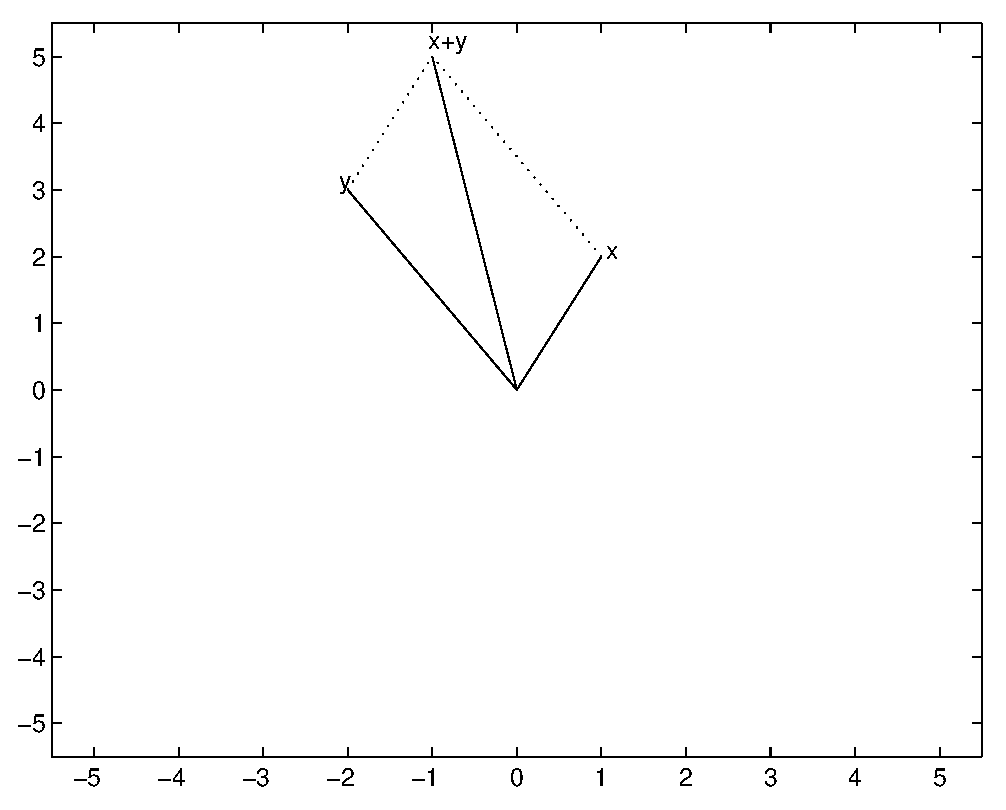
\psfig{file=figures/vec2.eps,width=2.5in}}
         \caption{Addition of two planar vectors.}
         \label{F:vec2}
\end{figure}


The parallelogram law (the diagonal of the parallelogram spanned
by $x$ and $y$ is $x+y$) is equally valid in three dimensions.
Use \Matlab to verify this statement by typing:
\begin{verbatim}
x = [1 0 2];
y = [-1 4 1];
addvec3(x,y)
\end{verbatim} \index{\computer!addvec3}
The parallelogram spanned by $x$ and $y$ in $\R^3$ is shown in
cyan; the diagonal $x+y$ is shown in blue.  See Figure~\ref{F:vec3}.   
To test your geometric intuition, make several choices of vectors $x$ and
$y$.  Note that one vertex of the parallelogram is always the
origin.

\begin{figure}[htb]
         \centerline{%
         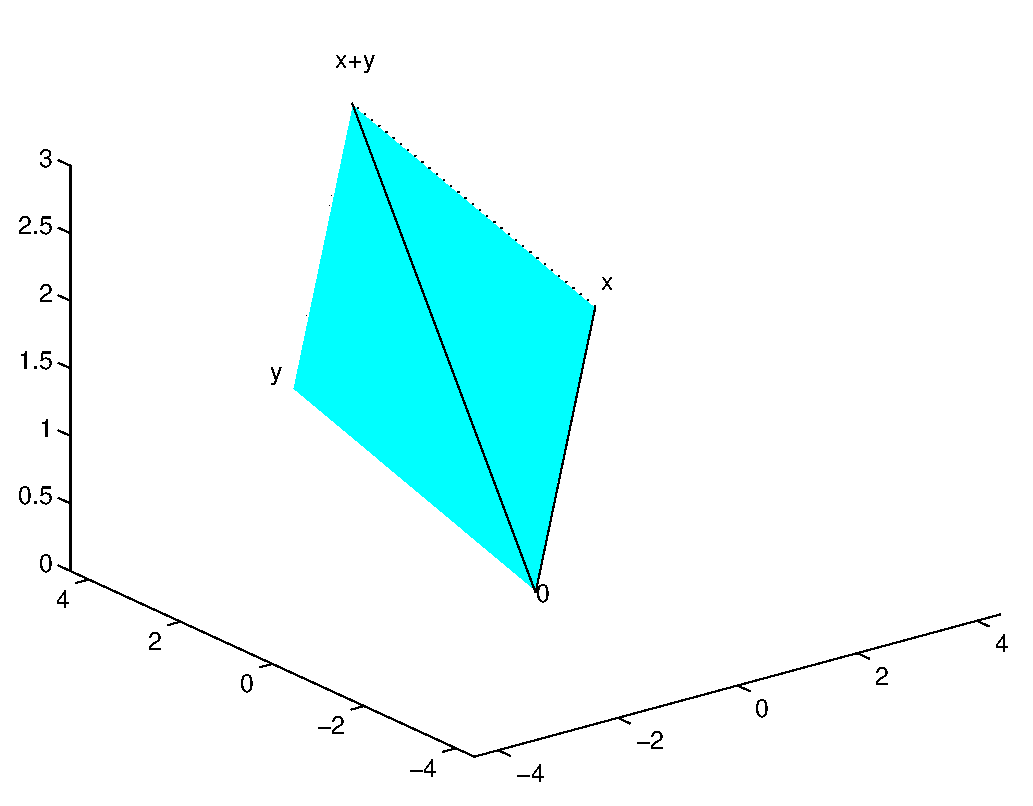
\psfig{file=figures/vec3.eps,width=3.0in}}
         \caption{Addition of two vectors in three dimensions.}
         \label{F:vec3}
\end{figure}


\subsection*{Geometry of Scalar Multiplication}

In all dimensions scalar multiplication\index{scalar
multiplication} just scales the length of the vector.  To
discuss this point we need to define the length of a vector.
View an $n$-vector $x=(x_1,\ldots,x_n)$ as a line segment from
the origin to the point $x$.  Using the Pythagorean theorem, it can
be shown that the {\em length\/}\index{length}\index{vector!length} 
or {\em norm\/}\index{norm}\index{vector!norm} of this line segment is:
\[
||x||  = \sqrt{x_1^2 + \cdots + x_n^2}.
\] \index{\computer:$||\cdot|| $}
\Matlab has the command {\tt norm} for finding the length of a
vector.  Test this by entering the $3$-vector
\begin{verbatim}
x = [1 4 2];
\end{verbatim}
Then type
\begin{verbatim}
norm(x)
\end{verbatim}  \index{\computer!norm}
\Matlab responds with:
\begin{verbatim}
ans =
    4.5826
\end{verbatim}
which is indeed approximately $\sqrt{1+4^2+2^2} = \sqrt{21}$.

Now suppose $r\in\R$ and $x\in\R^n$.  A calculation shows that
\begin{equation}  \label{E:lengths}
||rx||  = |r| ||x||.
\end{equation}
See Exercise~\ref{c1.4.9A}.  Note also that if $r$ is positive, 
then the direction of $rx$
is the same as that of $x$; while if $r$ is negative, then the
direction of $rx$ is opposite to the direction of $x$.  The
lengths of the vectors $3x$ and $-3x$ are each three times the
length of $x$ --- but these vectors point in opposite
directions.  Scalar multiplication by the scalar $0$ produces
the $0$ vector, the vector whose entries are all zero.

\subsection*{Dot Product and Angles}

The {\em dot product\/}\index{dot product} of two $n$-vectors
$x=(x_1,\ldots,x_n)$ and $y=(y_1,\ldots,y_n)$ is an important
operation on vectors.  It is defined by:
\begin{equation}  \label{e:dotproduct}
x\cdot y = x_1y_1 + \cdots + x_ny_n.
\end{equation}
Note that $x\cdot x$ is just $||x||^2$, the length of $x$
squared.

\Matlab also has a command for computing dot products of
$n$-vectors.  Type
\begin{verbatim}
x = [1 4 2];
y = [2 3 -1];
dot(x,y)
\end{verbatim}\index{\computer!dot}
\Matlab responds with the dot product of $x$ and $y$, namely,
\begin{verbatim}
ans =
    12
\end{verbatim}

One of the most important facts concerning dot products is the
one that states
\begin{equation} \label{dotprod=0}
x\cdot y = 0 \quad \mbox{if and only if} \quad \mbox{$x$ and $y$
are perpendicular}.
\end{equation}  \index{perpendicular}
Indeed, dot product also gives a way of numerically determining
the angle between $n$-vectors, as follows.
\begin{thm} \label{T:dotangle}
Let $\theta$ be the angle between two nonzero $n$-vectors $x$
and $y$.  Then
\begin{equation}  \label{e:dotproductang}
\cos \theta = \frac{x\cdot y}{||x|| ||y||}.
\end{equation}
\end{thm}
It follows that $\cos \theta=0$
if and only if $x\cdot y = 0$.  Thus \Ref{dotprod=0} is valid.

\proof  Theorem~\ref{T:dotangle} is just a restatement of the
{\em law of cosines\/}\index{law of cosines}.  Recall that the
law of cosines states that
\[
c^2 = a^2 + b^2 -2ab\cos\theta,
\]
where $a,b,c$ are the lengths of the sides of a triangle and $\theta$
is the interior angle opposite the side of length $c$.
In vector notation we can form a triangle two of whose sides are
given by $x$ and $y$ in $\R^n$.  The third side is just $x-y$ as
$x=y+(x-y)$, as in Figure~\ref{F:costri}.

\begin{figure}[htb]
     \centerline{%
     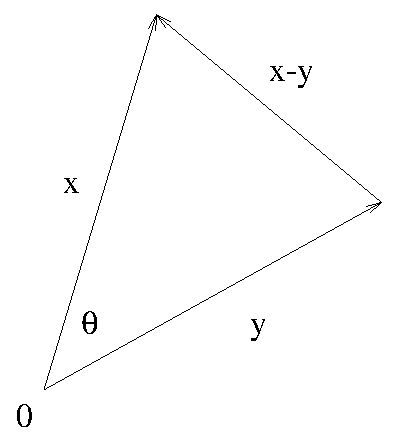
\psfig{file=figures/costri.eps,height=2.0in}}
     \caption{Triangle formed by vectors $x$ and $y$ with interior
	angle $\theta$.}
     \label{F:costri}
\end{figure}

It follows from the law of cosines that
\[
||x-y||^2 = ||x||^2 + ||y||^2 - 2||x|| ||y||  \cos\theta.
\]
We claim that
\[
||x-y||^2 = ||x||^2 + ||y||^2 -2x\cdot y.
\]
Assuming that the claim is valid, it follows that
\[
x\cdot y = ||x|| ||y||  \cos\theta,
\]
which proves the theorem.  Finally, compute
\begin{eqnarray*}
||x-y||^2 & = &(x_1-y_1)^2 + \cdots + (x_n-y_n)^2 \\
& = & (x_1^2-2x_1y_1+y_1^2) + \cdots + (x_n^2-2x_ny_n+y_n^2)\\
& = & (x_1^2+\cdots+x_n^2)-2(x_1y_1+\cdots+x_ny_n)+(y_1^2+\cdots+y_n^2)\\
& = & ||x||^2 -2x\cdot y + ||y||^2
\end{eqnarray*}
to verify the claim.   \qed

Theorem~\ref{T:dotangle} gives a numerically efficient method
for computing the angle\index{angle between vectors} between
vectors $x$ and $y$.  In \Matlab
this computation proceeds by typing
\begin{verbatim}
theta = acos(dot(x,y)/(norm(x)*norm(y)))
\end{verbatim} \index{\computer!acos}\index{\computer!dot}
where {\tt acos} is the inverse cosine of a number.
For example, using the $3$-vectors $x = (1,4,2)$ and $y =
(2,3,-1)$ entered previously, \Matlab responds with
\begin{verbatim}
theta =
    0.7956
\end{verbatim}
Remember that this answer is in radians\index{radians}.  To convert
this answer to degrees\index{degrees}, just multiply by $360$ and
divide by $2\pi$:
\begin{verbatim}
360*theta / (2*pi)
\end{verbatim}
to obtain the answer of $45.5847^\circ$.

\subsubsection{Area of Parallelograms}

Let $P$ be a parallelogram whose sides are the vectors $v$ and $w$ as
in Figure~\ref{F:parallel}.  Let $|P|$ denote the area of $P$.  As an
application of dot products \index{dot product} and
\Ref{e:dotproductang}, we calculate $|P|$. \index{parallelogram}
We claim that
\begin{equation}  \label{e:areaP}
|P|^2 = ||v||^2||w||^2 - (v\cdot w)^2.
\end{equation}
We verify \Ref{e:areaP} as follows.  Note that the area of $P$
is the same as the area of the rectangle $R$ also pictured in
Figure~\ref{F:parallel}.  The side lengths of $R$ are: $||v||$ and
$||w||\sin\theta$ where $\theta$ is the angle between $v$ and $w$.
A computation using \Ref{e:dotproductang} shows that
\begin{eqnarray*}
|R|^2 & = & ||v||^2 ||w||^2\sin^2\theta \\
& = & ||v||^2 ||w||^2(1-\cos^2\theta) \\
& = & ||v||^2 ||w||^2\left(1-\left(\frac{v\cdot w}{||v|| ||w||}
\right)^2\right)\\
& = & ||v||^2 ||w||^2 - (v\cdot w)^2,
\end{eqnarray*}
which establishes \Ref{e:areaP}.

\begin{figure}[htb]
     \centerline{%
     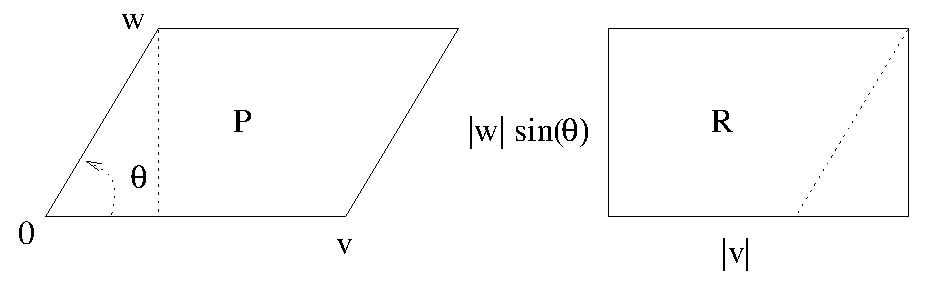
\psfig{file=figures/parallel.eps,width=3.5in}}
     \caption{Parallelogram $P$ beside rectangle $R$ with same area.}
     \label{F:parallel}
\end{figure}


\EXER

\TEXER

\noindent In Exercises~\ref{c1.4.8a} -- \ref{c1.4.8d}
compute the lengths of the given vectors.
\begin{exercise} \label{c1.4.8a}
$x=(3,0)$.
\end{exercise}
\begin{exercise} \label{c1.4.8b}
$x=(2,-1)$.
\end{exercise}
\begin{exercise} \label{c1.4.8c}
$x=(-1,1,1)$.
\end{exercise}
\begin{exercise} \label{c1.4.8d}
$x=(-1,0,2,-1,3)$.
\end{exercise}


\noindent In Exercises~\ref{c1.4.1a} -- \ref{c1.4.1c} determine
whether the given pair of vectors is perpendicular.
\begin{exercise} \label{c1.4.1a}
$x=(1,3)$ and $y=(3,-1)$.
\end{exercise}
\begin{exercise} \label{c1.4.1b}
$x=(2,-1)$ and $y=(-2,1)$.
\end{exercise}
\begin{exercise} \label{c1.4.1bb}
$x=(1,1,3,5)$ and $y=(1,-4,3,0)$.
\end{exercise}
\begin{exercise} \label{c1.4.1c}
$x=(2,1,4,5)$ and $y=(1,-4,3,-2)$.
\end{exercise}


\begin{exercise} \label{c1.4.2}
Find a real number $a$ so that the vectors
\[
x = (1,3,2) \AND y = (2,a,-6)
\]
are perpendicular.
\end{exercise}

\begin{exercise} \label{c1.4.3}
Find the lengths of the vectors $u=(2,1,-2)$ and $v=(0,1,-1)$,
and the angle between them.
\end{exercise}

\noindent In Exercises~\ref{c1.4.9a} -- \ref{c1.4.9f}
compute the dot product $x\cdot y$ for the given pair of vectors and 
the cosine of the angle between them.
\begin{exercise} \label{c1.4.9a}
$x=(2,0)$ and $y=(2,1)$.
\end{exercise}
\begin{exercise} \label{c1.4.9b}
$x=(2,-1)$ and $y=(1,2)$.
\end{exercise}
\begin{exercise} \label{c1.4.9c}
$x=(-1,1,4)$ and $y=(0,1,3)$.
\end{exercise}
\begin{exercise} \label{c1.4.9d}
$x=(-10,1,0)$ and $y=(0,1,20)$.
\end{exercise}
\begin{exercise} \label{c1.4.9e}
$x=(2,-1,1,3,0)$ and $y=(4,0,2,7,5)$.
\end{exercise}
\begin{exercise} \label{c1.4.9f}
$x=(5,-1,4,1,0,0)$ and $y=(-3,0,0,1,10,-5)$.
\end{exercise}

\begin{exercise}  \label{c1.4.9A}
Using the definition of length, verify that formula \Ref{E:lengths} 
is valid.
\end{exercise}


\CEXER

\begin{exercise} \label{c1.4.4}
Use {\tt addvec} and {\tt addvec3} to add vectors in $\R^2$ and
$\R^3$.  More precisely, enter pairs of $2$-vectors {\tt x} and {\tt y} 
of your choosing into \Matlabp, use {\tt addvec} to compute {\tt x+y},
and note the parallelogram formed by $0,x,y,x+y$.  Similarly, enter 
pairs of $3$-vectors and use {\tt addvec3}.
\end{exercise}

\begin{exercise} \label{c1.4.5}
Determine the vector of length $1$ that points in the same direction
as the vector
\[
x=(2,13.5,-6.7,5.23).
\]
\end{exercise}

\begin{exercise} \label{c1.4.5b}
Determine the vector of length $1$ that points in the same direction
as the vector
\[
y=(2.1,-3.5,1.5,1.3,5.2).
\]
\end{exercise}

\noindent In Exercises~\ref{c1.4.6a}-- \ref{c1.4.6c} find the angle in
degrees between the given pair of vectors.
\begin{exercise} \label{c1.4.6a}
$x=(2,1,-3,4)$ and $y=(1,1,-5,7)$.
\end{exercise}
\begin{exercise} \label{c1.4.6b}
$x=(2.43, 10.2,-5.27,\pi)$ and $y= (-2.2,0.33,4,-1.7)$.
\end{exercise}
\begin{exercise} \label{c1.4.6c}
$x=(1,-2,2,1,2.1)$ and $y=(-3.44,1.2,1.5,-2,-3.5)$.
\end{exercise}

\noindent In Exercises~\ref{c1.4.7a} -- \ref{c1.4.7b} let $P$ be the 
parallelogram generated by the given vectors $v$ and $w$ in $\R^3$.  
Compute the area of that parallelogram.
\begin{exercise} \label{c1.4.7a}
$v=(1,5,7)$ and $w=(-2,4,13)$.
\end{exercise}
\begin{exercise} \label{c1.4.7b}
$v=(2,-1,1)$ and $w=(-1,4,3)$.
\end{exercise}

\documentclass{ximera}

 

\usepackage{epsfig}

\graphicspath{
  {./}
  {figures/}
}

\usepackage{morewrites}
\makeatletter
\newcommand\subfile[1]{%
\renewcommand{\input}[1]{}%
\begingroup\skip@preamble\otherinput{#1}\endgroup\par\vspace{\topsep}
\let\input\otherinput}
\makeatother

\newcommand{\includeexercises}{\directlua{dofile("/home/jim/linearAlgebra/laode/exercises.lua")}}

%\newcounter{ccounter}
%\setcounter{ccounter}{1}
%\newcommand{\Chapter}[1]{\setcounter{chapter}{\arabic{ccounter}}\chapter{#1}\addtocounter{ccounter}{1}}

%\newcommand{\section}[1]{\section{#1}\setcounter{thm}{0}\setcounter{equation}{0}}

%\renewcommand{\theequation}{\arabic{chapter}.\arabic{section}.\arabic{equation}}
%\renewcommand{\thefigure}{\arabic{chapter}.\arabic{figure}}
%\renewcommand{\thetable}{\arabic{chapter}.\arabic{table}}

%\newcommand{\Sec}[2]{\section{#1}\markright{\arabic{ccounter}.\arabic{section}.#2}\setcounter{equation}{0}\setcounter{thm}{0}\setcounter{figure}{0}}

\newcommand{\Sec}[2]{\section{#1}}

\setcounter{secnumdepth}{2}
%\setcounter{secnumdepth}{1} 

%\newcounter{THM}
%\renewcommand{\theTHM}{\arabic{chapter}.\arabic{section}}

\newcommand{\trademark}{{R\!\!\!\!\!\bigcirc}}
%\newtheorem{exercise}{}

\newcommand{\dfield}{{\sf dfield9}}
\newcommand{\pplane}{{\sf pplane9}}

\newcommand{\EXER}{\section*{Exercises}}%\vspace*{0.2in}\hrule\small\setcounter{exercise}{0}}
\newcommand{\CEXER}{}%\vspace{0.08in}\begin{center}Computer Exercises\end{center}}
\newcommand{\TEXER}{} %\vspace{0.08in}\begin{center}Hand Exercises\end{center}}
\newcommand{\AEXER}{} %\vspace{0.08in}\begin{center}Hand Exercises\end{center}}

% BADBAD: \newcommand{\Bbb}{\bf}

\newcommand{\R}{\mbox{$\Bbb{R}$}}
\newcommand{\C}{\mbox{$\Bbb{C}$}}
\newcommand{\Z}{\mbox{$\Bbb{Z}$}}
\newcommand{\N}{\mbox{$\Bbb{N}$}}
\newcommand{\D}{\mbox{{\bf D}}}
\usepackage{amssymb}
%\newcommand{\qed}{\hfill\mbox{\raggedright$\square$} \vspace{1ex}}
%\newcommand{\proof}{\noindent {\bf Proof:} \hspace{0.1in}}

\newcommand{\setmin}{\;\mbox{--}\;}
\newcommand{\Matlab}{{M\small{AT\-LAB}} }
\newcommand{\Matlabp}{{M\small{AT\-LAB}}}
\newcommand{\computer}{\Matlab Instructions}
\newcommand{\half}{\mbox{$\frac{1}{2}$}}
\newcommand{\compose}{\raisebox{.15ex}{\mbox{{\scriptsize$\circ$}}}}
\newcommand{\AND}{\quad\mbox{and}\quad}
\newcommand{\vect}[2]{\left(\begin{array}{c} #1_1 \\ \vdots \\
 #1_{#2}\end{array}\right)}
\newcommand{\mattwo}[4]{\left(\begin{array}{rr} #1 & #2\\ #3
&#4\end{array}\right)}
\newcommand{\mattwoc}[4]{\left(\begin{array}{cc} #1 & #2\\ #3
&#4\end{array}\right)}
\newcommand{\vectwo}[2]{\left(\begin{array}{r} #1 \\ #2\end{array}\right)}
\newcommand{\vectwoc}[2]{\left(\begin{array}{c} #1 \\ #2\end{array}\right)}

\newcommand{\ignore}[1]{}


\newcommand{\inv}{^{-1}}
\newcommand{\CC}{{\cal C}}
\newcommand{\CCone}{\CC^1}
\newcommand{\Span}{{\rm span}}
\newcommand{\rank}{{\rm rank}}
\newcommand{\trace}{{\rm tr}}
\newcommand{\RE}{{\rm Re}}
\newcommand{\IM}{{\rm Im}}
\newcommand{\nulls}{{\rm null\;space}}

\newcommand{\dps}{\displaystyle}
\newcommand{\arraystart}{\renewcommand{\arraystretch}{1.8}}
\newcommand{\arrayfinish}{\renewcommand{\arraystretch}{1.2}}
\newcommand{\Start}[1]{\vspace{0.08in}\noindent {\bf Section~\ref{#1}}}
\newcommand{\exer}[1]{\noindent {\bf \ref{#1}}}
\newcommand{\ans}{}
\newcommand{\matthree}[9]{\left(\begin{array}{rrr} #1 & #2 & #3 \\ #4 & #5 & #6
\\ #7 & #8 & #9\end{array}\right)}
\newcommand{\cvectwo}[2]{\left(\begin{array}{c} #1 \\ #2\end{array}\right)}
\newcommand{\cmatthree}[9]{\left(\begin{array}{ccc} #1 & #2 & #3 \\ #4 & #5 &
#6 \\ #7 & #8 & #9\end{array}\right)}
\newcommand{\vecthree}[3]{\left(\begin{array}{r} #1 \\ #2 \\
#3\end{array}\right)}
\newcommand{\cvecthree}[3]{\left(\begin{array}{c} #1 \\ #2 \\
#3\end{array}\right)}
\newcommand{\cmattwo}[4]{\left(\begin{array}{cc} #1 & #2\\ #3
&#4\end{array}\right)}

\newcommand{\Matrix}[1]{\ensuremath{\left(\begin{array}{rrrrrrrrrrrrrrrrrr} #1 \end{array}\right)}}

\newcommand{\Matrixc}[1]{\ensuremath{\left(\begin{array}{cccccccccccc} #1 \end{array}\right)}}



\renewcommand{\labelenumi}{\theenumi)}
\newenvironment{enumeratea}%
{\begingroup
 \renewcommand{\theenumi}{\alph{enumi}}
 \renewcommand{\labelenumi}{(\theenumi)}
 \begin{enumerate}}
 {\end{enumerate}\endgroup}



\newcounter{help}
\renewcommand{\thehelp}{\thesection.\arabic{equation}}

%\newenvironment{equation*}%
%{\renewcommand\endequation{\eqno (\theequation)* $$}%
%   \begin{equation}}%
%   {\end{equation}\renewcommand\endequation{\eqno \@eqnnum
%$$\global\@ignoretrue}}

%\input{psfig.tex}

\author{Martin Golubitsky and Michael Dellnitz}

%\newenvironment{matlabEquation}%
%{\renewcommand\endequation{\eqno (\theequation*) $$}%
%   \begin{equation}}%
%   {\end{equation}\renewcommand\endequation{\eqno \@eqnnum
% $$\global\@ignoretrue}}

\newcommand{\soln}{\textbf{Solution:} }
\newcommand{\exercap}[1]{\centerline{Figure~\ref{#1}}}
\newcommand{\exercaptwo}[1]{\centerline{Figure~\ref{#1}a\hspace{2.1in}
Figure~\ref{#1}b}}
\newcommand{\exercapthree}[1]{\centerline{Figure~\ref{#1}a\hspace{1.2in}
Figure~\ref{#1}b\hspace{1.2in}Figure~\ref{#1}c}}
\newcommand{\para}{\hspace{0.4in}}

\renewenvironment{solution}{\suppress}{\endsuppress}

\ifxake
\newenvironment{matlabEquation}{\begin{equation}}{\end{equation}}
\else
\newenvironment{matlabEquation}%
{\let\oldtheequation\theequation\renewcommand{\theequation}{\oldtheequation*}\begin{equation}}%
  {\end{equation}\let\theequation\oldtheequation}
\fi

\makeatother


\title{c2.tex}

\begin{document}
\begin{abstract}
BADBAD
\end{abstract}
\maketitle

\chapter{Solving Linear Equations} \label{lineq}

\normalsize

The primary motivation for the study of vectors and matrices is based
on the study of solving systems of linear equations.  The algorithms
that enable us to find solutions are themselves based on certain kinds
of matrix manipulations.  In these algorithms, matrices serve as a
shorthand for calculation, rather than as a basis for a theory.  We will
see later that these matrix manipulations do lead to a rich theory of how
to solve systems of linear equations.  But our first step is just to see
how these equations are actually solved.

We begin with a discussion in Section~\ref{S:2.1} of how to write systems
of linear equations in terms of matrices.  We also show by example how
complicated writing down the answer to such systems can be.  In
Section~\ref{S:2.2}, we recall that solution sets to systems of linear
equations in two and three variables are lines and planes.

The best known and probably the most efficient method for solving
systems of linear equations (especially with a moderate to large number
of unknowns) is Gaussian elimination.  The idea behind this method,
which is introduced in Section~\ref{S:Gauss}, is to manipulate matrices
by elementary row operations to reduced echelon form.  It is then possible
just to look at the reduced echelon form matrix and to read off the
solutions to the linear system, if any.  The process of reading off the
solutions is formalized in Section~\ref{S:2.4}; see Theorem~\ref{number}.
Our discussion of solving linear equations is presented with equations
whose coefficients are real numbers --- though most of our examples have
just integer coefficients.  The methods work just as well with complex
numbers, and this generalization is discussed in Section~\ref{S:specialcoeff}.

Throughout this chapter, we alternately discuss the theory and show how
calculations that are tedious when done by hand can easily be performed
by computer using \Matlabp.  The chapter ends with a proof of the
uniqueness of row echelon form (a topic of theoretical importance) in
Section~\ref{S:uniquerowechelon}.  This section is included mainly for
completeness and need not be covered on a first reading.


\section{Systems of Linear Equations and Matrices}
\label{S:2.1}

It is a simple exercise to solve the system of two equations
\begin{equation} \label{small}
\arraycolsep 2pt
\begin{array}{rcrcr}
 x & + & y & = & 7 \\
-x & + & 3y & = & 1
\end{array}
\end{equation}
to find that $x=5$ and $y=2$.  One way to solve
system \Ref{small} is to add the two equations, obtaining
\[
4y=8;
\]
hence $y=2$.  Substituting $y=2$ into the $1^{st}$ equation in
\Ref{small} yields $x=5$.

This system of equations can be solved in a more algorithmic
fashion by solving the $1^{st}$ equation in \Ref{small} for $x$
as
\[
x = 7 - y,
\]
and substituting this answer into the $2^{nd}$ equation in
\Ref{small}, to obtain
\[
-(7-y) +3y = 1.
\]
This equation simplifies to:
\[
4y = 8.
\]
Now proceed as before.

\subsection*{Solving Larger Systems by Substitution}

In contrast to solving the simple system of two equations,
it is less clear how to solve a complicated system of five
equations such as:
\begin{equation}    \label{big}
\arraycolsep 2pt
\begin{array}{rcrcrcrcrcrl}
 5x_1 & - & 4x_2 & + & 3x_3 & - & 6x_4 & + & 2x_5 & = &   4  & \\
 2x_1 & + &  x_2 & - &  x_3 & - &  x_4 & + &  x_5 & = &   6  & \\
  x_1 & + & 2x_2 & + &  x_3 & + &  x_4 & + & 3x_5 & = &  19  & \\
-2x_1 & - &  x_2 & - &  x_3 & + &  x_4 & - &  x_5 & = & -12  & \\
  x_1 & - & 6x_2 & + &  x_3 & + &  x_4 & + & 4x_5 & = &   4  & \!
.
\end{array}
\end{equation}
The algorithmic method used to solve \Ref{small} can be expanded
to produce a method, called {\em substitution\/},
\index{substitution} for solving larger systems. We describe the
substitution method as it applies to \Ref{big}.  Solve the
$1^{st}$ equation in \Ref{big} for $x_1$, obtaining
\begin{equation} \label{x1}
x_1 = \frac{4}{5}  + \frac{4}{5}x_2 - \frac{3}{5}x_3
   + \frac{6}{5}x_4 - \frac{2}{5}x_5.
\end{equation}
Then substitute the right hand side of \Ref{x1} for $x_1$ in the
remaining four equations in \Ref{big} to obtain a new system of
four equations in the four variables $x_2$,$x_3$,$x_4$,$x_5$.
This procedure eliminates the variable $x_1$.  Now proceed
inductively --- solve the $1^{st}$ equation in the new system
for $x_2$ and substitute this expression into the remaining
three equations to obtain a system of three equations in three
unknowns.  This step eliminates the variable $x_2$.  Continue by
substitution to eliminate the variables $x_3$ and $x_4$, and
arrive at a simple equation in $x_5$ --- which can be solved.
Once $x_5$ is known, then $x_4$, $x_3$, $x_2$, and $x_1$ can be
found in turn.

\subsection*{Two Questions}

\begin{itemize}
\item Is it realistic to expect to complete the substitution
procedure without making a mistake in arithmetic?
\item Will this procedure work --- or will some unforeseen
difficulty arise?
\end{itemize}

Almost surely, attempts to solve \Ref{big} by hand,
using the substitution procedure, will lead to arithmetic
errors.  However, computers and software have developed to the
point where solving a system such as \Ref{big} is routine.  In
this text, we use the software package \Matlab to illustrate
just how easy it has become to solve equations such as \Ref{big}.

The answer to the second question requires knowledge of the
{\em theory\/} of linear algebra.  In fact, no difficulties will
develop when trying to solve the particular system \Ref{big}
using the substitution algorithm.  We discuss why later.

\subsection*{Solving Equations by \Matlab}

We begin by discussing the information that is needed by \Matlab
to solve \Ref{big}.  The computer needs to know that there are
five equations in five unknowns --- but it does not need to keep
track of the unknowns $(x_1,x_2,x_3,x_4,x_5)$ by name.  Indeed,
the computer just needs to know the {\em matrix of
coefficients\/} \index{matrix!coefficient} in \Ref{big}
\begin{equation*}  \label{bigmatrix}
\left(
\begin{array}{rrrrr}
 5 & -4 &  3 & -6 &  2 \\
 2 &  1 & -1 & -1 &  1 \\
 1 &  2 &  1 &  1 &  3 \\
-2 & -1 & -1 &  1 & -1 \\
 1 & -6 &  1 &  1 &  4
\end{array}
\right)
\end{equation*}
and the {\em vector\/} on the right hand side of \Ref{big}
\begin{equation*} \label{bigRHS}
\left(
\begin{array}{r}
  4 \\
  6 \\
 19 \\
-12 \\
  4
\end{array}
\right).
\end{equation*}

We now describe how we enter this information into \Matlabp.  To
reduce the drudgery and to allow us to focus on ideas, the entries
in equations having a $*$ after their label
(such as \Ref{bigmatrix}*) have been entered in the {\tt laode}
toolbox. This information can be accessed as follows.  After
starting your \Matlab session, type
\begin{verbatim}
e2_1_4
\end{verbatim}
followed by a carriage return.  This instruction tells \Matlab to
load equation \Ref{bigmatrix} of Chapter~\ref{lineq}.  The matrix of
coefficients is now available in \Matlabp; note that this matrix is
stored in the $5\times 5$ array {\tt A}.  What should appear is:
\begin{verbatim}
A =
     5    -4     3    -6     2
     2     1    -1    -1     1
     1     2     1     1     3
    -2    -1    -1     1    -1
     1    -6     1     1     4
\end{verbatim}
Indeed, comparing this result with \Ref{bigmatrix}, we see that
{\tt A} contains precisely the same information.

Since the label \Ref{bigRHS} is followed by a `$*$', we can enter
the vector in \Ref{bigRHS} into \Matlab by typing
\begin{verbatim}
e2_1_5
\end{verbatim}
Note that the right hand side of \Ref{big} is stored in the vector {\tt b}.
\Matlab should have responded with
\begin{verbatim}
b =
     4
     6
    19
   -12
     4
\end{verbatim}
Now \Matlab has all the information it needs to solve the system
of equations given in \Ref{big}.  To have \Matlab solve this
system, type
\begin{verbatim}
x = A\b
\end{verbatim}
\index{\computer!$\backslash$}to obtain
\begin{verbatim}
x =
    5.0000
    2.0000
    3.0000
    4.0000
    1.0000
\end{verbatim}
This answer is interpreted as follows: the five values of the
unknowns $x_1$,$x_2$,$x_3$,$x_4$,$x_5$ are stored in the vector
$x$; that is,
\begin{equation} \label{answer1}
 x_1 = 5,\quad x_2 = 2,\quad x_3 = 3,\quad x_4 = 4,\quad x_5 = 1.
\end{equation}
The reader may verify that \Ref{answer1} is indeed a solution of
\Ref{big} by substituting the values in \Ref{answer1} into the
equations in \Ref{big}.

\subsection*{Changing Entries in \Matlab}

\Matlab also permits access to single components of $x$.  For
instance, type
\begin{verbatim}
x(5)
\end{verbatim}
and the $5^{th}$ entry of $x$ is displayed,
\begin{verbatim}
ans =
    1.0000
\end{verbatim}
We see that the component {\tt x(i)} of {\tt x} corresponds to
the component $x_i$ of the vector $x$ where $i=1,2,3,4,5$.
Similarly, we can access the entries of the coefficient matrix
\index{matrix!coefficient} {\tt A}.
For instance, by typing
\begin{verbatim}
A(3,4)
\end{verbatim}
\Matlab responds with
\begin{verbatim}
ans =
    1
\end{verbatim}

It is also possible to change an individual entry in either a vector
or a matrix.  For example, if we enter
\begin{verbatim}
A(3,4) = -2
\end{verbatim}  \index{\computer!A(3,4)}
we obtain a new matrix {\tt A} which when displayed is:
\begin{verbatim}
A =
     5    -4     3    -6     2
     2     1    -1    -1     1
     1     2     1    -2     3
    -2    -1    -1     1    -1
     1    -6     1     1     4
\end{verbatim}
Thus the command {\tt A(3,4) = -2} changes the entry in the
$3^{rd}$ row, $4^{th}$ column of {\tt A} from $1$ to $-2$.
In other words, we have now entered into \Matlab the
information that is needed to solve the system of equations
\[
\arraycolsep 2pt
\begin{array}{rcrcrcrcrcrl}
 5x_1 & - & 4x_2 & + & 3x_3 & - &  6x_4 & + & 2x_5 & = &   4  & \\
 2x_1 & + &  x_2 & - &  x_3 & - &   x_4 & + &  x_5 & = &   6  & \\
  x_1 & + & 2x_2 & + &  x_3 & - &  2x_4 & + & 3x_5 & = &  19  & \\
-2x_1 & - &  x_2 & - &  x_3 & + &   x_4 & - &  x_5 & = & -12  & \\
x_1 & - & 6x_2 & + & x_3 & + & x_4 & + & 4x_5 & = & 4 & \! .
\end{array}
\]
As expected, this change in the coefficient matrix results in a
change in the solution of system \Ref{big}, as well.  Typing
\begin{verbatim}
x = A\b
\end{verbatim}
now leads to the solution
\begin{verbatim}
x =
    1.9455
    3.0036
    3.0000
    1.7309
    3.8364
\end{verbatim}
that is displayed to an accuracy of four decimal places.

In the next step, change {\tt A} as follows:
\begin{verbatim}
A(2,3) = 1
\end{verbatim}
The new system of equations is:
\begin{equation}  \label{incon}
\arraycolsep 2pt
\begin{array}{rcrcrcrcrcrl}
 5x_1 & - & 4x_2 & + & 3x_3 & - &  6x_4 & + & 2x_5 & = &   4  & \\
 2x_1 & + &  x_2 & + &  x_3 & - &   x_4 & + &  x_5 & = &   6  & \\
  x_1 & + & 2x_2 & + &  x_3 & - &  2x_4 & + & 3x_5 & = &  19  & \\
-2x_1 & - &  x_2 & - &  x_3 & + &   x_4 & - &  x_5 & = & -12  & \\
  x_1 & - & 6x_2 & + &  x_3 & + &   x_4 & + & 4x_5 & = &   4  & \!
.
\end{array}
\end{equation}
The command
\begin{verbatim}
x = A\b
\end{verbatim}  \index{\computer!$\backslash$}
now leads to the message
\begin{verbatim}
Warning: Matrix is singular to working precision.

x =
   Inf
   Inf
   Inf
   Inf
   Inf
\end{verbatim}  \index{\computer!inf}
Obviously, something is {\em wrong\/}; \Matlab cannot find a
solution to this system of equations!  Assuming that \Matlab is
working correctly, we have shed light on one of our previous
questions: the method of substitution described by \Ref{x1} need
{\em not\/} always lead to a solution, even though the method
does work for system \Ref{big}.  Why?  As we will see, this is
one of the questions that is answered by the theory of linear
algebra.  In the case of \Ref{incon}, it is fairly easy to see
what the difficulty is: the second and fourth equations
have the form $y=6$ and $-y=-12$, respectively.

\vspace{0.1in}

\noindent {\bf Warning:}  The \Matlab command
\begin{verbatim}
x = A\b
\end{verbatim}
may give an error message similar to the previous one.  When
this happens, one must approach the answer with caution.

\EXER


\TEXER

\noindent In Exercises~\ref{c2.1.8a} -- \ref{c2.1.8c} find solutions
to the given system of linear equations.
\begin{exercise} \label{c2.1.8a}
\[
\begin{array}{rcrcr}
 2x & - & y & = & 0 \\
 3x &   &   & = & 6 \end{array}
\]
\end{exercise}
\begin{exercise} \label{c2.1.8b}
\[
\begin{array}{rcrcrcr}
 3x & - & 4y &   &    & = & 2\\
    &   & 2y & + & z  & = & 1\\
    &   &    &   & 3z & = & 9 \end{array}
\]
\end{exercise}
\begin{exercise} \label{c2.1.8c}
\[
\begin{array}{rcrcr}
 -2x & + &  y & = &  9 \\
  3x & + & 3y & = & -9 \end{array}
\]
\end{exercise}

\begin{exercise} \label{c2.1.8A}
Write the coefficient matrices for each of the systems of linear equations 
given in Exercises~\ref{c2.1.8a} -- \ref{c2.1.8c}.
\end{exercise}

\begin{exercise} \label{c2.1.9}
Neither of the following systems of three equations in three
unknowns has a unique solution --- but for different
reasons.  Solve these systems and explain why these systems
cannot be solved uniquely.
\[
\mbox{(a) }\; \begin{array}{rcrcrcr}
  x & - &  y &   &    & = &  4\\
  x & + & 3y & - & 2z & = & -6\\
 4x & + & 2y & - & 3z & = &  1
\end{array} \AND
\mbox{(b) }\; \begin{array}{rcrcrcr}
 2x & - & 4y & + & 3z & = &  4\\
 3x & - & 5y & + & 3z & = &  5\\
    &   & 2y & - & 3z & = & -4
\end{array}
\]
\end{exercise}

\begin{exercise} \label{c2.1.10}
Last year Dick was twice as old as Jane.  Four years ago the
sum of Dick's age and Jane's age was twice Jane's age now.  How
old are Dick and Jane?

{\bf Hint:} Rewrite the two statements
as linear equations in $D$ --- Dick's age now --- and $J$ ---
Jane's age now.  Then solve the system of linear equations.
\end{exercise}

\begin{exercise} \label{c2.1.11}
\begin{itemize}
\item[(a)] Find a quadratic polynomial $p(x) = ax^2 + bx + c$
satisfying $p(0) = 1$, $p(1) = 5$, and $p(-1) = -5$.
\item[(b)] Prove that for every triple of real numbers $L$, $M$,
and $N$, there is a quadratic polynomial satisfying $p(0) = L$,
$p(1) = M$, and $p(-1) = N$.
\item[(c)] Let $x_1,x_2,x_3$ be three unequal real
numbers and let $A_1,A_2,A_3$ be three real numbers.  Show
that finding a quadratic polynomial $q(x)$ that satisfies
$q(x_i) = A_i$ is equivalent to solving a system of three
linear equations.
\end{itemize}
\end{exercise}

\CEXER

\begin{exercise} \label{c2.1.1}
Using \Matlab type the commands {\tt e2\_1\_8} and {\tt e2\_1\_9}
to load the matrices:
\begin{equation*}
A = \left(
\begin{array}{rrrrrr}
   -5.6 &  0.4 & -9.8 &  8.6 &  4.0 & -3.4\\
   -9.1 &  6.6 & -2.3 &  6.9 &  8.2 &  2.7\\
    3.6 & -9.3 & -8.7 &  0.5 &  5.2 &  5.1\\
    3.6 & -8.9 & -1.7 & -8.2 & -4.8 &  9.8\\
    8.7 &  0.6 &  3.7 &  3.1 & -9.1 & -2.7\\
   -2.3 &  3.4 &  1.8 & -1.7 &  4.7 & -5.1
\end{array}
\right)
\end{equation*}
and the {\em vector\/}
\begin{equation*}
b = \left(
\begin{array}{r}
    9.7\\
    4.5\\
    5.1\\
    3.0\\
   -8.5\\
    2.6
\end{array}
\right)
\end{equation*}
Solve the corresponding system of linear equations.
\end{exercise}

\begin{exercise} \label{c2.1.2}
Matrices are entered in \Matlab as follows. To enter
the $2\times 3$ matrix $A$, type {\tt A = [ -1 1 2; 4 1 2]}.
Enter this matrix into \Matlabp; the displayed matrix should be
\begin{verbatim}
A =
    -1     1     2
     4     1     2
\end{verbatim}
Now change the entry in the $2^{nd}$ row, $1^{st}$ column to
$-5$.
\end{exercise}

\begin{exercise} \label{c2.1.3}
Column vectors with $n$ entries are viewed by \Matlab as
$n\times 1$ matrices.  Enter the vector {\tt b = [1; 2; -4]}.
Then change the $3^{rd}$ entry in {\tt b} to $13$.
\end{exercise}


\begin{exercise} \label{c2.1.4}
This problem illustrates some of the different ways that \Matlab
displays numbers using the {\tt format long}, the {\tt format short} and
the {\tt format rational} commands.

Use \Matlab to solve the following system of equations
\[
\arraycolsep 2pt
\begin{array}{rcrcrcrl}
 2x_1 & - & 4.5x_2 & + & 3.1x_3 & = &   4.2  & \\
  x_1 & + &  x_2 & + &  x_3 & = &  -5.1  & \\
  x_1 & - & 6.2x_2 & + &  x_3 & = &  1.3  & \! .
\end{array}
\]
You may change the format of your answer in \Matlabp.  For
example, to print your result with an accuracy of $15$ digits
type {\tt format long} \index{\computer!format!long} and redisplay the
answer.  Similarly, to print your result as fractions type {\tt
format rational} \index{\computer!format!rational} and redisplay your
answer.
\end{exercise}

\begin{exercise} \label{c2.1.5}
Enter the following matrix and vector into \Matlab
\begin{verbatim}
 A = [ 1 0 -1 ; 2 5 3 ; 5 -1 0];
 b = [ 1; 1; -2];
\end{verbatim}
and solve the corresponding system of linear equations by typing
\begin{verbatim}
x = A\b
\end{verbatim}
Your answer should be
\begin{verbatim}
x =
   -0.2000
    1.0000
   -1.2000
\end{verbatim}
Find an integer for the entry in the $2^{nd}$ row, $2^{nd}$ column
of $A$ so that the solution
\begin{verbatim}
x = A\b
\end{verbatim}
is not defined.  {\bf Hint:} The answer is an integer between
$-4$ and $4$.
\end{exercise}

\begin{exercise} \label{c2.1.6}
The \Matlab command {\tt rand(m,n)}\index{\computer!rand} defines
matrices with random
entries between $0$ and $1$.  For example, the command {\tt A =
rand(5,5)} generates a random $5\times 5$ matrix, whereas the
command {\tt b = rand(5,1)} generates a column vector with $5$
random entries.  Use these commands to construct several systems
of linear equations and then solve them.
\end{exercise}

\begin{exercise} \label{c2.1.7}
Suppose that the four substances $S_1$, $S_2$, $S_3$, $S_4$
contain the following percentages of vitamins A, B, C and F by
weight
\begin{center}
\begin{tabular}{|c||r|r|r|r|}
\hline
Vitamin   & $S_1$ & $S_2$ & $S_3$ & $S_4$\\
\hline
 A & 25\% &    19\% &    20\% &    3\% \\
 B &  2\% &    14\% &     2\% &   14\% \\
 C &  8\% &     4\% &     1\% &     0\% \\
 F & 25\% &    31\% &    25\% &    16\% \\
\hline
\end{tabular}
\end{center}
Mix the substances $S_1$, $S_2$, $S_3$ and $S_4$ so that the
resulting mixture contains precisely $3.85$ grams of vitamin A,
$2.30$ grams of vitamin B, $0.80$ grams of vitamin C, and $5.95$
grams of vitamin F.  How many grams of each substance have to be
contained in the mixture?

Discuss what happens if we require that the resulting mixture contains
$2.00$ grams of vitamin B instead of $2.30$ grams.
\end{exercise}



\section{The Geometry of Low-Dimensional Solutions}
\label{S:2.2}

In this section we discuss how to use \Matlab graphics to solve
systems of linear equations in two and three unknowns.  We begin
with two dimensions.

\subsection*{Linear Equations in Two Dimensions}

The set of all solutions to the equation
\begin{equation} \label{2x-y=6}
2x - y = 6
\end{equation}
is a straight line in the $xy$ plane; this line
has slope $2$ and $y$-intercept equal to $-6$.  We can use
\Matlab to plot the solutions to this equation --- though some
understanding of the way \Matlab works is needed.

The {\tt plot} command in \Matlab plots a sequence of points in
the plane, as follows.  Let $X$ and $Y$ be $n$ vectors. Then
\begin{verbatim}
plot(X,Y)
\end{verbatim} \index{\computer!plot}
will plot the points $(X(1),Y(1))$, $(X(2),Y(2))$, \ldots,
$(X(n),Y(n))$ in the $xy$-plane.  

To plot points on the line
\Ref{2x-y=6} we need to enter the $x$-coordinates of the points
we wish to plot.  If we want to plot a hundred points, we would
be facing a tedious task.  \Matlab has a command to simplify
this task. Typing
\begin{verbatim}
x = linspace(-5,5,100);
\end{verbatim} \index{\computer!linspace}
produces a vector $x$ with $100$ entries with the $1^{st}$ entry
equal to $-5$, the last entry equal to $5$, and the remaining $98$ 
entries equally spaced between $-5$ and $5$.  \Matlab has another command 
that allows us to create a vector of points {\tt x}.  In this command
we specify the distance between points rather than the number of 
points.  That command is:
\begin{verbatim}
x = -5:0.1:5;
\end{verbatim}
Producing {\tt x} by either command is acceptable.

Typing
\begin{verbatim}
y = 2*x - 6;
\end{verbatim}
produces a vector whose entries correspond to the
$y$-coordinates of points on the line \Ref{2x-y=6}.  Then typing
\begin{verbatim}
plot(x,y)
\end{verbatim}
produces the desired plot.  It is useful to label the axes on
this figure, which is accomplished by typing
\begin{verbatim}
xlabel('x')
ylabel('y')
\end{verbatim} \index{\computer!xlabel}\index{\computer!ylabel}

We can now use \Matlab to solve the equation \Ref{small}
graphically.  Recall that \Ref{small} is:
\[
\arraycolsep 2pt
\begin{array}{rcrcr}
 x & + &  y & = & 7 \\
-x & + & 3y & = & 1
\end{array}
\]
A solution to this system of equations is a point that lies on
both lines in the system.  Suppose that we search for a solution
to this system that has an $x$-coordinate between $-3$ and $7$.
Then type the commands
\begin{verbatim}
x = linspace(-3,7,100);
y = 7 - x;
plot(x,y)
xlabel('x')
ylabel('y')
hold on
y = (1 + x)/3;
plot(x,y)
axis('equal')
grid
\end{verbatim} \index{\computer!hold} \index{\computer!axis('equal')}
\index{\computer!grid}
The \Matlab command {\tt hold on} tells \Matlab to keep the
present figure and to add the information that follows to that figure.
The command {\tt axis('equal')} instructs \Matlab to make unit distances
on the $x$ and $y$ axes equal.  The last \Matlab command superimposes
grid lines. See Figure~\ref{lineint}.  From this figure
you can see that the solution to this system is $(x,y)=(5,2)$, which
we already knew.

\begin{figure}[htb]
                       \centerline{%
                       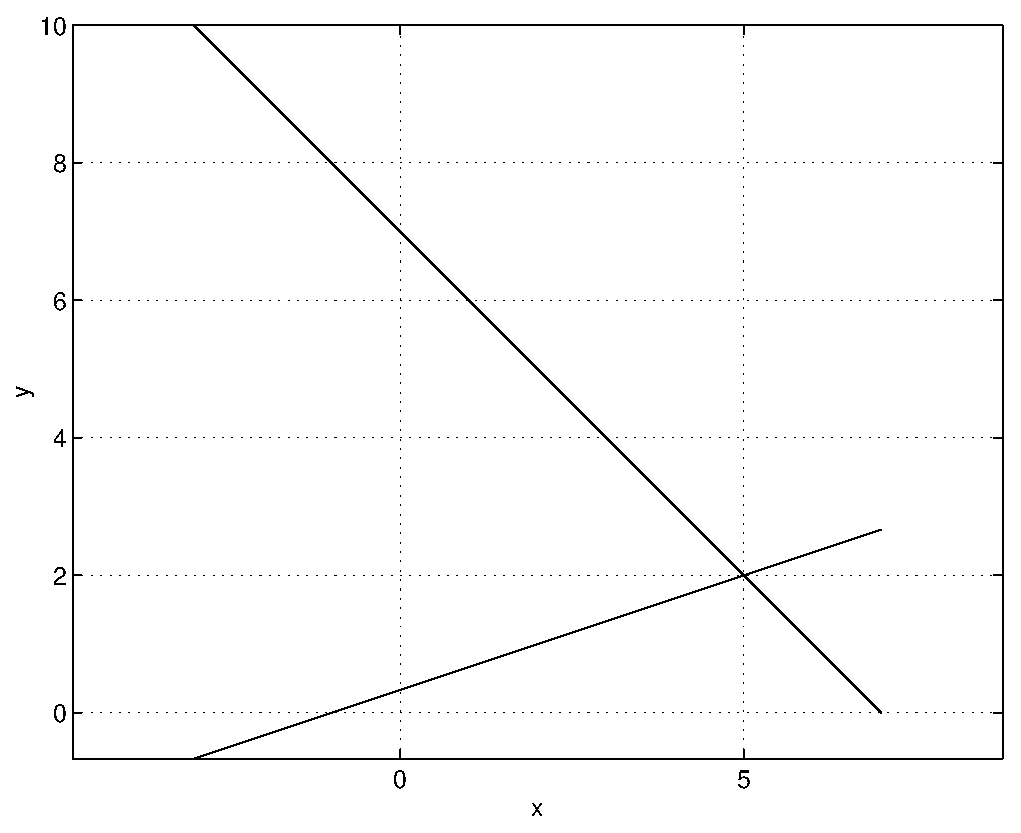
\psfig{file=figures/lineint.eps,width=3.5in}}
                       \caption{Graph of equations in \protect\Ref{small}}
                       \label{lineint}
\end{figure}


There are several principles that follow from this exercise.
\begin{itemize}
\item   Solutions to a single linear equation in two variables
form a straight line.
\item Solutions to two linear equations in two unknowns lie at
the intersection of two straight lines in the plane.
\end{itemize}
It follows that the solution to two linear equations in two
variables is a single point if the lines are not parallel.  If
these lines are parallel and unequal, then there are no
solutions, as there are no points of intersection.

\subsection*{Linear Equations in Three Dimensions}

We begin by observing that the set of all solutions to a linear
equation in three variables forms a plane\index{plane}.  More
precisely, the solutions to the equation
\begin{equation} \label{abcd}
ax+by+cz=d
\end{equation}
form a plane that is perpendicular to the vector $(a,b,c)$ ---
assuming of course that the vector $(a,b,c)$ is nonzero.

This fact is most easily proved using the {\em dot product\/}.
Recall from Chapter~\ref{chap:prelim} \Ref{e:dotproduct} that
the dot product\index{dot product} is defined by
\[
X\cdot Y = x_1y_1+x_2y_2+x_3y_3,
\]
where $X=(x_1,x_2,x_3)$ and $Y=(y_1,y_2,y_3)$.  We recall from
Chapter~\ref{chap:prelim} \Ref{dotprod=0} the following important
fact concerning dot products:
\[
X\cdot Y = 0
\]
if and only if the vectors $X$ and $Y$ are perpendicular.

Suppose that $N=(a,b,c)\neq 0$.  Consider the plane that is perpendicular
to the {\em normal vector\/}\index{normal vector} $N$ and that contains the
point $X_0$.  If the point $X$ lies in that plane, then $X-X_0$ is
perpendicular to $N$; that is,
\begin{equation} \label{XX_0}
(X-X_0)\cdot N = 0.
\end{equation}
If we use the notation
\[
X=(x,y,z) \quad \mbox{ and } \quad X_0=(x_0,y_0,z_0),
\]
then \Ref{XX_0} becomes
\[
a(x-x_0)+b(y-y_0)+c(z-z_0)=0.
\]
Setting
\[
d=ax_0 + by_0 + cz_0
\]
puts equation \Ref{XX_0} into the form \Ref{abcd}.  In this way
we see that the set of solutions to a single linear equation in
three variables forms a plane.  See Figure~\ref{F:plane}.

\begin{figure}[htb]
              \centerline{%
              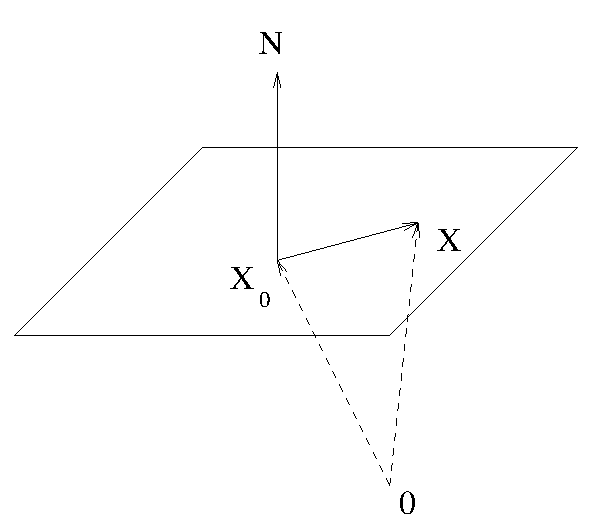
\psfig{file=figures/plane.eps,width=2.5in}}
              \caption{The plane containing $X_0$ and perpendicular to $N$.}
              \label{F:plane}
\end{figure}


We now use \Matlab to visualize the planes that are solutions to
linear equations.  Plotting an equation in three dimensions in
\Matlab follows a structure similar to the planar plots.
Suppose that we wish to plot the solutions to the equation
\begin{equation} \label{-2x+3y+z=2}
-2x+3y+z=2.
\end{equation}
We can rewrite \Ref{-2x+3y+z=2} as
\[
z=2x-3y+2.
\]
It is this function that we actually graph by typing the
commands
\begin{verbatim}
[x,y] = meshgrid(-5:0.5:5);
z = 2*x - 3*y + 2;
surf(x,y,z)
\end{verbatim} \index{\computer!meshgrid}  \index{\computer!surf}
The first command tells \Matlab to create a square grid in the
$xy$-plane.  Grid points are
equally spaced between $-5$ and $5$ at intervals of $0.5$ on
both the $x$ and $y$ axes. The second command tells \Matlab to
compute the $z$ value of the solution to \Ref{-2x+3y+z=2} at
each grid point.  The third command tells \Matlab to graph the
surface containing the points $(x,y,z)$.  See
Figure~\ref{F:p1int}.

\begin{figure}[htb]
              \centerline{%
              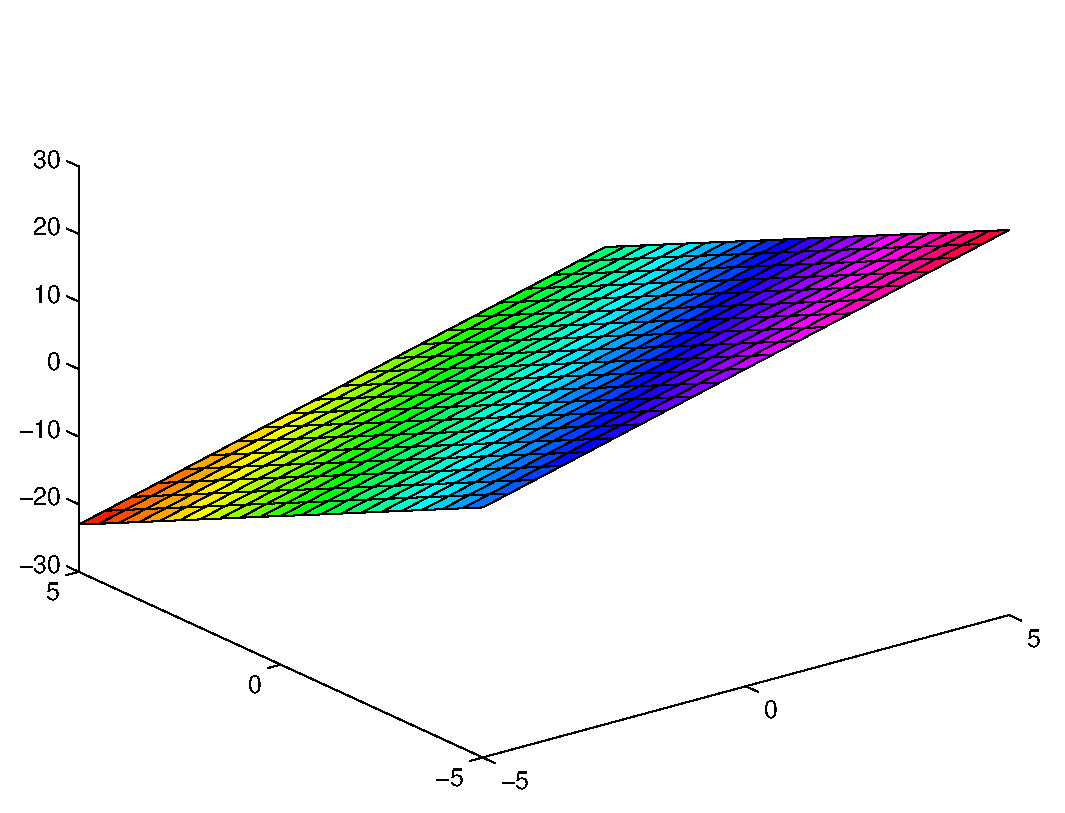
\psfig{file=figures/p1int.eps,width=3.0in}}
              \caption{Graph of \protect\Ref{-2x+3y+z=2}.}
              \label{F:p1int}
\end{figure}


We can now see that solutions to a system of two linear
equations in three unknowns consists of points that lie
simultaneously on two planes.  As long as the normal vectors to
these planes are not parallel, the intersection of the two
planes will be a line in three dimensions.  Indeed, consider the
equations
\begin{eqnarray*}
-2x + 3y + z & = & 2 \\
 2x - 3y + z & = & 0.
\end{eqnarray*}
We can graph the solution using \Matlab, as follows. We continue
from the previous graph by typing
\begin{verbatim}
hold on
z = -2*x + 3*y;
surf(x,y,z)
\end{verbatim}
The result, which illustrates that the intersection of two planes
in $\R^3$ is generally a line, is shown in Figure~\ref{F:p2int}.

\begin{figure}[htb]
              \centerline{%
              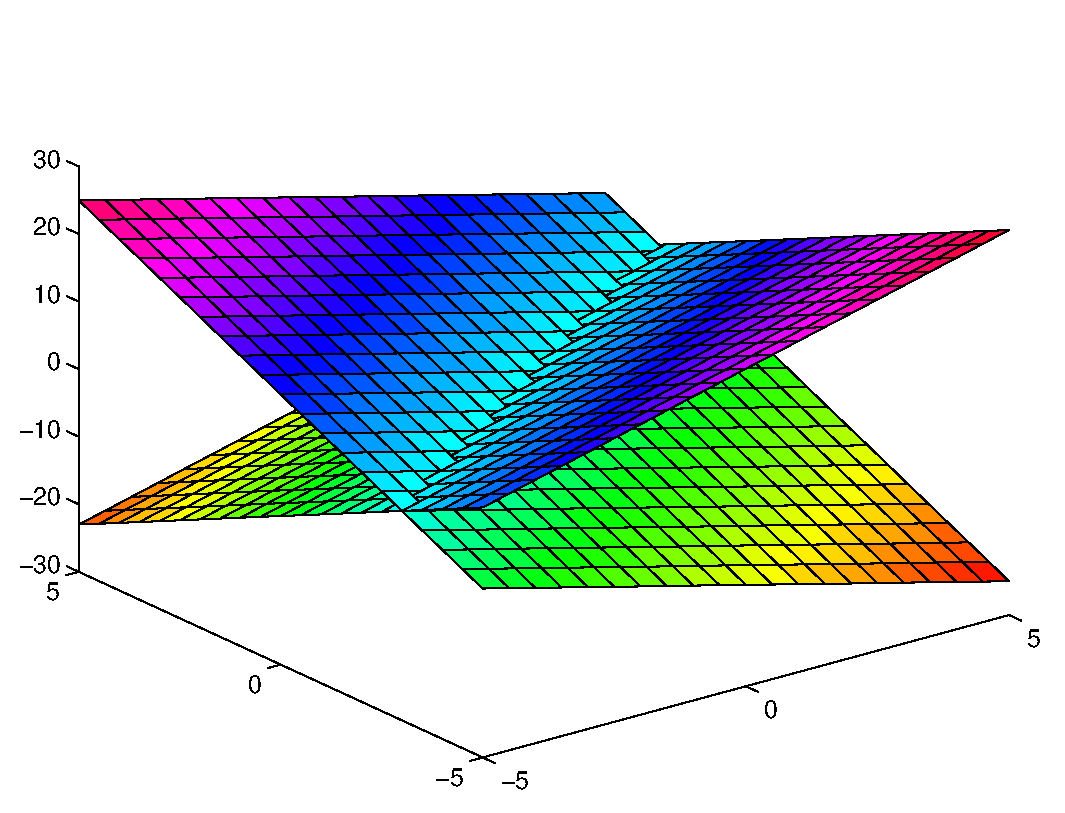
\psfig{file=figures/p2int.eps,width=3.0in}}
              \caption{Line of intersection of two planes.}
              \label{F:p2int}
\end{figure}

We can now see geometrically that the solution to three
simultaneous linear equations in three unknowns will generally
be a point --- since generally three planes in three space
intersect in a point.  To visualize this intersection, as shown in
Figure~\ref{F:p3int}, we extend the previous system of equations to
\begin{eqnarray*}
-2x +   3y + z & = & 2 \\
 2x -   3y + z & = & 0\\
-3x + 0.2y + z & = & 1.
\end{eqnarray*}
Continuing in \Matlab type
\begin{verbatim}
z = 3*x - 0.2*y + 1;
surf(x,y,z)
\end{verbatim}

\begin{figure}[htb]
              \centerline{%
              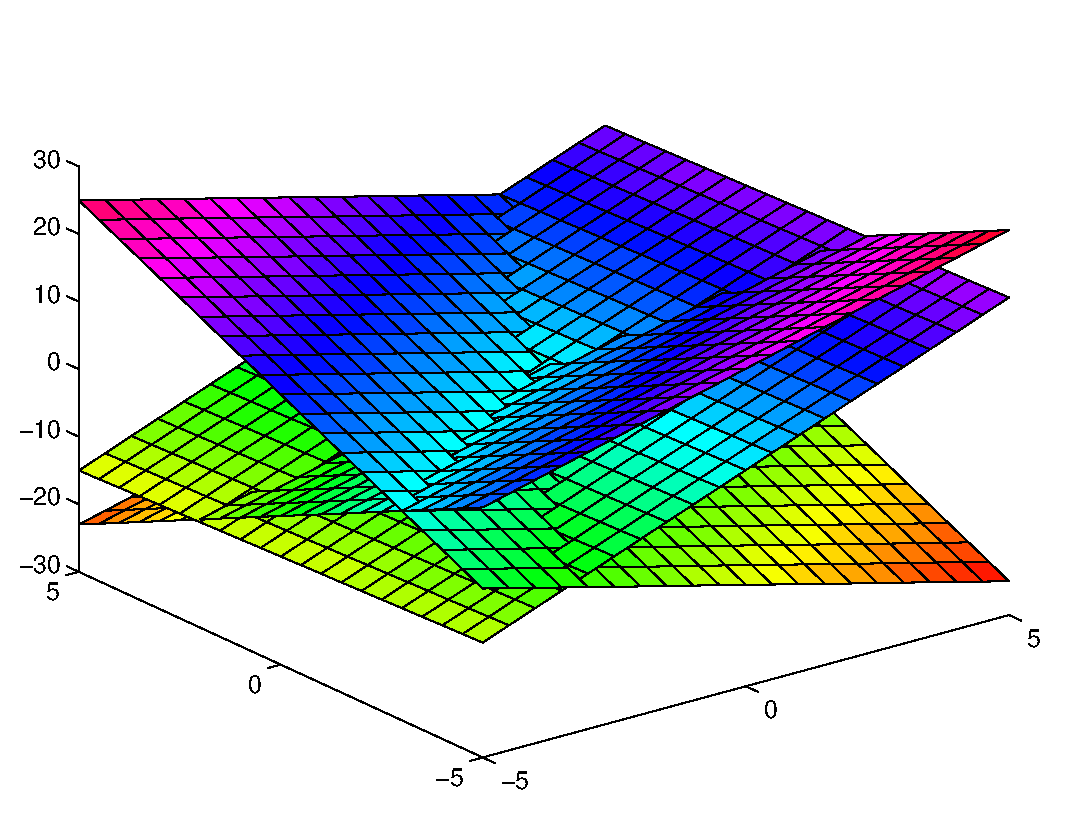
\psfig{file=figures/p3int.eps,width=3.0in}}
              \caption{Point of intersection of three planes.}
              \label{F:p3int}
\end{figure}

Unfortunately, visualizing the point of intersection of these
planes geometrically does not really help to get an accurate
numerical value of the coordinates of this intersection point.  
However, we can use \Matlab to solve this system accurately.
Denote the $3\times 3$ matrix of coefficients by {\tt A}, the 
vector of coefficients on the right hand side by {\tt b}, and 
the solution by {\tt x}.  Solve the system in \Matlab by typing
\begin{verbatim}
A = [ -2 3 1; 2 -3 1; -3 0.2 1];
b = [2; 0; 1];
x = A\b
\end{verbatim}
The point of intersection of the three planes is at
\begin{verbatim}
x =
    0.0233
    0.3488
    1.0000
\end{verbatim}

Three planes in three dimensional space need not intersect in a
single point.  For example, if two of the planes are parallel
they need not intersect at all.  The normal vectors must point
in {\em independent\/} directions to
guarantee that the intersection is a point.  Understanding the
notion of independence (it is more complicated than just not
being parallel) is part of the subject of linear algebra.
\Matlab returns ``{\tt Inf}'', which we have seen previously,
when these normal vectors are (approximately) dependent. For
example, consider Exercise~\ref{c2.2.10}.

\subsection*{Plotting Nonlinear Functions in \Matlab}

Suppose that we want to plot the graph of a nonlinear function of
a single variable, such as
\begin{equation}  \label{E:quadex}
y = x^2 - 2x + 3
\end{equation}
on the interval $[-2,5]$ using \Matlabp.  There is a difficulty:  How
do we enter the term $x^2$?  For example, suppose that we type
\begin{verbatim}
x = linspace(-2,5);
y = x*x - 2*x + 3;
\end{verbatim}
Then \Matlab responds with
\begin{verbatim}
??? Error using ==> *
Inner matrix dimensions must agree.
\end{verbatim}
The problem is that in \Matlab the variable {\tt x} is a vector of
100 equally spaced points {\tt x(1), x(2), \ldots, x(100)}.  What we
really need is a vector consisting of entries {\tt x(1)*x(1), x(2)*x(2),
\ldots, x(100)*x(100)}.  \Matlab has the facility to perform this
operation automatically and the syntax for the operation is {\tt .*}
rather than {\tt *}.  So typing
\begin{verbatim}
x = linspace(-2,5);
y = x.*x - 2*x + 3;
plot(x,y)
\end{verbatim}\index{\computer!{\tt .*}}
produces the graph of \Ref{E:quadex} in Figure~\ref{F:quadex}.
\begin{figure}[htb]
              \centerline{%
              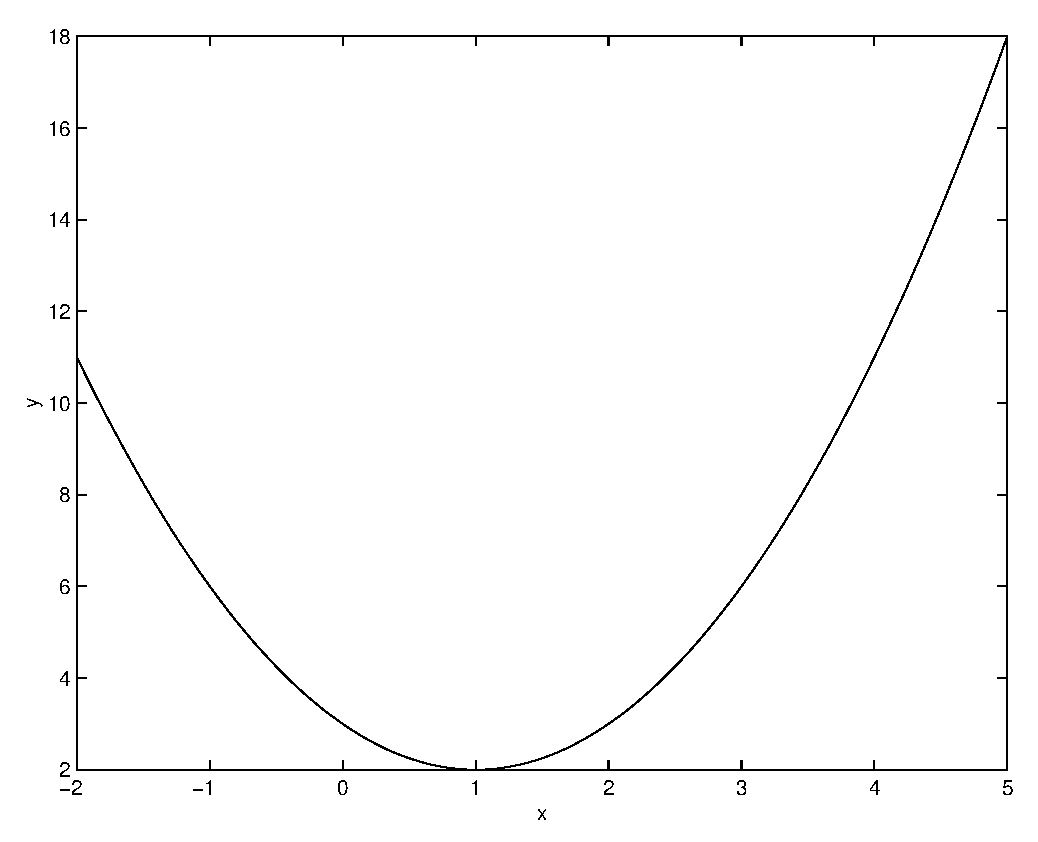
\psfig{file=figures/quadex.eps,width=3.0in}}
              \caption{Graph of $y = x^2 - 2x + 3$.}
              \label{F:quadex}
\end{figure}
In a similar fashion, \Matlab has the `dot' operations of
{\tt ./}\index{\computer!{\tt ./}},
{\tt .$\backslash$}, and  .\^{}\index{\computer!.\^{}}, as well
as {\tt .*}.

\EXER



\TEXER

\begin{exercise} \label{c2.2.5}
Find the equation for the plane perpendicular to the vector $(2,3,1)$
and containing the point $(-1,-2,3)$.
\end{exercise}

\begin{exercise} \label{c2.2.6}
Determine three systems of two linear equations in two unknowns
so that the first system has a unique solution, the second
system has an infinite number of solutions, and the third system
has no solutions.
\end{exercise}

\begin{exercise} \label{c2.2.7}
Write the equation of the plane through the origin containing the
vectors $(1,0,1)$ and $(2,-1,2)$.
\end{exercise}

\begin{exercise} \label{c2.2.8}
Find a system of two linear equations in three
unknowns whose solution set is the line consisting of scalar
multiples of the vector $(1,2,1)$.
\end{exercise}

\begin{exercise} \label{c2.2.9}
\begin{itemize}
\item[(a)] Find a vector $u$ normal to the plane $2x+2y+z=3$.
\item[(b)] Find a vector $v$ normal to the plane $x+y+2z=4$.
\item[(c)] Find the cosine of the angle between the vectors $u$ and $v$.
Use \Matlab to find the angle in degrees.
\end{itemize}
\end{exercise}

\begin{exercise} \label{c2.2.10}
Determine graphically the geometry of the set of solutions to the
system of equations in the three unknowns $x,y,z$:
\[
\begin{array}{rcrcr}
  x & + & 3z  & = & 1\\
 3x & - &  z  & = & 1\\
    &   &  z  & = & 2
\end{array}
\]
by sketching the plane of solutions for each equation individually.
Describe in words why there are no solutions to this system.
(Use \Matlab graphics to verify your sketch.  Note that you should
enter the last equation as {\tt z = 2 - 0*x - 0*y} and the first two
equations with {\tt 0*y} terms.  Try different views --- but include
{\tt view([0 1 0])} as one view.)
\end{exercise}

\CEXER

\begin{exercise} \label{c2.2.1}
Use \Matlab to solve graphically the planar system of linear
equations
\[
\arraycolsep 2pt
\begin{array}{rcrcr}
 x & + & 4y & = & -4 \\
4x & + & 3y & = &  4
\end{array}
\]
to an accuracy of two decimal points.

{\bf Hint:} The \Matlab command {\tt zoom on}\index{\computer!zoom}
allows us to
view the plot in a window whose axes are one-half those of
original.  Each time you click with the mouse on a point,
the axes' limits are halved and centered at the designated
point. Coupling {\tt zoom on} with {\tt grid on} allows you
to determine approximate numerical values for the intersection
point.
\end{exercise}

\begin{exercise} \label{c2.2.2}
Use \Matlab to solve graphically the planar system of linear
equations
\[
\arraycolsep 2pt
\begin{array}{rcrcr}
4.23x & + & 0.023y & = & -1.1 \\
1.65x & - & 2.81y & = &  1.63
\end{array}
\]
to an accuracy of two decimal points.
\end{exercise}


\begin{exercise} \label{c2.2.3}
Use \Matlab to find an approximate graphical solution to the
three dimensional system of linear equations
\[
\begin{array}{rcrcrcr}
 3x & - & 4y & + & 2z  & = & -11\\
 2x & + & 2y & + &  z  & = &   7\\
 -x & + &  y & - & 5z  & = &   7.
\end{array}
\]
Then use \Matlab to find an exact solution.
\end{exercise}


\begin{exercise} \label{c2.2.4}
Use \Matlab to determine graphically the geometry of the set of
solutions to the system of equations:
\[
\begin{array}{rcrcrcr}
  x & + & 3y & + & 4z  & = & 5\\
 2x & + &  y & + &  z  & = & 1\\
-4x & + & 3y & + & 5z  & = & 7.
\end{array}
\]
Attempt to use \Matlab to find an exact solution to this system
and discuss the implications of your calculations.

{\bf Hint:} After setting up the graphics display in \Matlabp,
you can use the command {\tt view([0,1,0])} \index{\computer!view} to get
a better view of the solution point.
\end{exercise}

\begin{exercise} \label{c2.2.a5}
Use \Matlab to graph the function $y = 2 - x\sin(x^2-1)$ on the interval
$[-2,3]$.  How many relative maxima does this function have on this interval?
\end{exercise}


\section{Gaussian Elimination}  \label{S:Gauss}

A general system of $m$ {\em linear\/} equations \index{linear}
in $n$ unknowns has the form
\begin{equation}    \label{general}
\arraycolsep 2pt
\begin{array}{rcrcrcrcrl}
 a_{11}x_1 & + & a_{12}x_2 & + & \cdots & + & a_{1n}x_n & = &   b_1
& \\
 a_{21}x_1 & + & a_{22}x_2 & + & \cdots & + & a_{2n}x_n & = &   b_2
& \\
        & \vdots &      & \vdots &    & \vdots &     & \vdots &
  & \\
 a_{m1}x_1 & + & a_{m2}x_2 & + & \cdots & + & a_{mn}x_n & = &   b_m
& .
\end{array}
\end{equation}
The entries $a_{ij}$ and $b_i$ are constants.  Our task is to find
a method for solving \Ref{general} for the variables
$x_1,\ldots,x_n$.

\subsection*{Easily Solved Equations}

Some systems are easily solved.  The system of three
equations ($m=3$) in three unknowns ($n=3$)
\begin{equation}
\begin{array}{rcrcrcrl} \label{examp3}
  x_1 & + & 2x_2 & + & 3x_3 & = &  10  & \\
      &   &  x_2 & - & \frac{1}{5}x_3 & = & \frac{7}{5}  & \\
      &   &      &   &  x_3 & = &   3  & \\
\end{array}
\end{equation}
is one example.  The $3^{rd}$ equation states that $x_3=3$.
Substituting this value into the $2^{nd}$ equation allows us to
solve the $2^{nd}$ equation for $x_2=2$.  Finally, substituting
$x_2=2$ and $x_3=3$ into the $1^{st}$ equation allows us to
solve for $x_1=-3$.  The process that we have just described is
called {\em back substitution\/}.\index{back substitution}

Next, consider the system of two equations ($m=2$) in three
unknowns ($n=3$):
\begin{equation}  \label{e23}
\begin{array}{rcrcrcrl}
  x_1 & + & 2x_2 & + & 3x_3 & = &  10  & \\
      &   &      &   &  x_3 & = &   3  & \! . \\
\end{array}
\end{equation}
The $2^{nd}$ equation in \Ref{e23} states that $x_3=3$.
Substituting
this value into the $1^{st}$ equation leads to the equation
\[
x_1 = 1-2x_2.
\]
We have shown that every solution to \Ref{e23} has the form
$(x_1,x_2,x_3)=(1-2x_2,x_2,3)$ and that every vector
$(1-2x_2,x_2,3)$ is a solution of \Ref{e23}.  Thus, there is an
infinite number of solutions to \Ref{e23}, and these solutions
can be parameterized by one number $x_2$.

\subsection*{Equations Having No Solutions}

Note that the system of equations
\begin{eqnarray*}
x_1 - x_2 = 1\\
x_1 - x_2 = 2
\end{eqnarray*}
has no solutions.

\begin{Def}
A linear system of equations is {\em inconsistent\/} if the
system has no solutions and {\em consistent\/} if the system
does have solutions.
\end{Def} \index{consistent} \index{inconsistent}

As discussed in the previous section, \Ref{incon} is an example
of a linear system that \Matlab cannot solve.  In fact, that
system is inconsistent --- inspect the $2^{nd}$ and $4^{th}$
equations in \Ref{incon}.

Gaussian elimination is an algorithm for finding all solutions
to a system of linear equations by reducing the given system to
ones like \Ref{examp3} and \Ref{e23}, that are easily solved by
back substitution.  Consequently, Gaussian elimination can also be
used to determine whether a system is consistent or inconsistent.

\subsection*{Elementary Equation Operations}

There are three ways to change a system of equations without
changing the set of solutions; Gaussian elimination
\index{Gaussian elimination} is based on this observation.  The
three elementary operations are:
\begin{enumerate}
\item   Swap two equations.
\item   Multiply a single equation by a nonzero number.
\item   Add a scalar multiple of one equation to another.
\end{enumerate}

We begin with an example:
\begin{equation}
\begin{array}{rcrcrcrl}
  x_1 & + & 2x_2 & + & 3x_3 & = &  10  & \\
  x_1 & + & 2x_2 & + &  x_3 & = &   4  & \\
 2x_1 & + & 9x_2 & + & 5x_3 & = &  27  & .\\
\end{array}
\end{equation}
Gaussian elimination works by eliminating variables from the
equations in a fashion similar to the substitution method in the
previous section.  To begin, eliminate the variable $x_1$ from
all but the $1^{st}$ equation, as follows.  Subtract the
$1^{st}$ equation from the $2^{nd}$, and subtract twice the
$1^{st}$ equation from the $3^{rd}$, obtaining:
\begin{equation}
\begin{array}{rcrcrcrl}
  x_1 & + & 2x_2 & + & 3x_3 & = &  10  & \\
      &   &      &   &-2x_3 & = &  -6  & \\
      &   & 5x_2 & - &  x_3 & = &   7  & .\\
\end{array}
\end{equation}
Next, swap the $2^{nd}$ and $3^{rd}$ equations, so that
the coefficient of $x_2$ in the new $2^{nd}$ equation is nonzero.
This yields
\begin{equation}
\begin{array}{rcrcrcrl}
  x_1 & + & 2x_2 & + & 3x_3 & = &  10  & \\
      &   & 5x_2 & - &  x_3 & = &   7  & \\
      &   &      &   &-2x_3 & = &  -6  & .\\
\end{array}
\end{equation}
Now, divide the $2^{nd}$ equation by $5$ and the $3^{rd}$
equation by $-2$ to obtain a system of equations identical to
our first example \Ref{examp3}, which we solved by back
substitution.


\subsection*{Augmented Matrices}

The process of performing Gaussian elimination when the number
of equations is greater than two or three is painful.  The
computer, however, can help with the manipulations.  We begin by
introducing the {\em augmented matrix\/}. \index{matrix!augmented}
The augmented matrix associated with \Ref{general} has
$m$ rows and $n+1$ columns and is written as:
\begin{equation}  \label{augmented}
\left(
\begin{array}{rrrr|r}
 a_{11} & a_{12} & \cdots & a_{1n} &  b_1 \\
 a_{21} & a_{22} & \cdots & a_{2n} &  b_2 \\
 \vdots & \vdots &        & \vdots & \vdots \\
 a_{m1} & a_{m2} & \cdots & a_{mn} &  b_m
\end{array}
\right)
\end{equation}
The augmented matrix contains all of the information that is
needed to solve system \Ref{general}.

\subsection*{Elementary Row Operations} \index{elementary row
operations}

The elementary operations used in Gaussian elimination
can be interpreted as {\em row operations\/} on
the augmented matrix, as follows:
\begin{enumerate}
\item   Swap two rows.
\item   Multiply a single row by a nonzero number.
\item   Add a scalar multiple of one row to another.
\end{enumerate}
We claim that by using these elementary row operations
intelligently, we can always solve a consistent linear system
--- indeed, we can determine when a linear system is consistent
or inconsistent.  The idea is to perform elementary row
operations in such a way that the new augmented matrix has zero
entries below the diagonal.

We describe this process inductively.  Begin with the $1^{st}$
column.  We assume for now that some entry in this column is
nonzero.  If $a_{11}=0$, then swap two rows so that the
number $a_{11}$ is nonzero.  Then divide the $1^{st}$ row by
$a_{11}$ so that the leading entry in that row is $1$.  Now
subtract $a_{i1}$ times the $1^{st}$ row from the $i^{th}$ row
for each row $i$ from $2$ to $m$.  The end result is that the
$1^{st}$ column has a $1$ in the $1^{st}$ row and a $0$ in every
row below the $1^{st}$.  The result is
\[
\left(\begin{array}{cccc}  1 & * & \cdots & * \\
0 & * & \cdots & * \\ \vdots & \vdots & \vdots & \vdots \\
0 & * & \cdots & * \end{array} \right).
\]


Next we consider the $2^{nd}$ column.  We assume that some entry
in that column below the $1^{st}$ row is nonzero.  So, if
necessary, we can swap two rows below the $1^{st}$ row so
that the entry $a_{22}$ is nonzero.  Then we divide the $2^{nd}$
row by $a_{22}$ so that its leading nonzero entry is $1$.  Then
we subtract appropriate multiples of the $2^{nd}$ row from each
row below the $2^{nd}$ so that all the entries in the $2^{nd}$
column below the $2^{nd}$ row are $0$.  The result is
\[
\left(\begin{array}{cccc}  1 & * & \cdots & * \\
0 & 1 & \cdots & * \\ \vdots & \vdots & \vdots & \vdots \\
0 & 0 & \cdots & * \end{array} \right).
\]

Then we continue with the $3^{rd}$ column.  That's the idea.  However,
does this process always work and what happens if all of the entries
in a column are zero?  Before answering these questions we do
experimentation with \Matlabp.

\subsection*{Row Operations in \Matlab}\index{elementary row
operations!in \protect\Matlab}

In \Matlab the $i^{th}$ row of a matrix {\tt A} is specified by
{\tt A(i,:)}.  Thus to replace the $5^{th}$ row of a matrix {\tt
A} by twice itself, we need only type:
\begin{verbatim}
A(5,:) = 2*A(5,:)
\end{verbatim}
In general, we can replace the $i^{th}$ row of the matrix
{\tt A} by $c$ times itself by typing
\begin{verbatim}
A(i,:) = c*A(i,:)
\end{verbatim}
Similarly, we can divide the $i^{th}$ row of the matrix {\tt A}
by the nonzero number $c$ by typing
\begin{verbatim}
A(i,:) = A(i,:)/c
\end{verbatim}

The third elementary row operation is performed similarly.
Suppose we want to add $c$ times the $i^{th}$ row to the
$j^{th}$ row, then we type
\begin{verbatim}
A(j,:) = A(j,:) + c*A(i,:)
\end{verbatim}
For example, subtracting $3$ times the $7^{th}$ row from the
$4^{th}$ row of the matrix {\tt A} is accomplished by typing:
\begin{verbatim}
A(4,:) = A(4,:) - 3*A(7,:)
\end{verbatim}

The first elementary row operation, swapping two rows, requires
a different kind of \Matlab command.  In \Matlabp, the $i^{th}$
and $j^{th}$ rows of the matrix {\tt A} are permuted by the
command
\begin{verbatim}
A([i j],:) = A([j i],:)
\end{verbatim}
So, to swap the $1^{st}$ and $3^{rd}$ rows of the matrix
{\tt A}, we type
\begin{verbatim}
A([1 3],:) = A([3 1],:)
\end{verbatim}  \index{\computer!A([1 3],:)}

\subsection*{Examples of Row Reduction in \Matlab}

Let us see how the row operations can be used in \Matlabp.  As
an example, we consider the augmented matrix
\begin{equation*}  \label{examp4}
\left(
\begin{array}{rrrr|r}
 1  &  3  &  0  & -1  &  -8\\
 2  &  6  & -4  &  4  &   4\\
 1  &  0  & -1  & -9  & -35\\
 0  &  1  &  0  &  3  &  10
\end{array}
\right)
\end{equation*}

We enter this information into \Matlab by typing
\begin{verbatim}
e2_3_8
\end{verbatim}
which produces the result
\begin{verbatim}
A =
     1     3     0    -1    -8
     2     6    -4     4     4
     1     0    -1    -9   -35
     0     1     0     3    10
\end{verbatim}

We now perform Gaussian elimination on {\tt A}, and then solve the 
resulting system by back substitution.  Gaussian elimination uses 
elementary row operations to set the entries that are in the lower 
left part of {\tt A} to zero. These entries are indicated by
numbers in the following matrix:
\begin{verbatim}
    *     *     *     *     *
    2     *     *     *     *
    1     0     *     *     *
    0     1     0     *     *
\end{verbatim}

Gaussian elimination \index{Gaussian elimination} works
inductively.  Since the first entry in the matrix $A$ is equal
to $1$, the first step in Gaussian elimination is to set to zero
all entries in the $1^{st}$ column below the $1^{st}$ row.  We
begin by eliminating the {\tt 2} that is the first entry in the
$2^{nd}$ row of {\tt A}.  We replace the $2^{nd}$ row by the
$2^{nd}$ row minus twice the $1^{st}$ row.  To accomplish this
elementary row operation, we type
\begin{verbatim}
A(2,:) = A(2,:) - 2*A(1,:)
\end{verbatim}
and the result is
\begin{verbatim}
A =
     1     3     0    -1    -8
     0     0    -4     6    20
     1     0    -1    -9   -35
     0     1     0     3    10
\end{verbatim}
In the next step, we eliminate the {\tt 1} from the entry in the
$3^{rd}$ row, $1^{st}$ column of {\tt A}.  We do this by
typing
\begin{verbatim}
A(3,:) = A(3,:) - A(1,:)
\end{verbatim}
which yields
\begin{verbatim}
A =
     1     3     0    -1    -8
     0     0    -4     6    20
     0    -3    -1    -8   -27
     0     1     0     3    10
\end{verbatim}

Using elementary row operations, we have now set the entries
in the $1^{st}$ column below the $1^{st}$ row to $0$.  Next,
we alter the $2^{nd}$ column.  We begin by swapping
the $2^{nd}$ and $4^{th}$ rows so that the leading nonzero entry
in the $2^{nd}$ row is $1$.   To accomplish this swap, we type
\begin{verbatim}
A([2 4],:) = A([4 2],:)
\end{verbatim}
and obtain
\begin{verbatim}
A =
     1     3     0    -1    -8
     0     1     0     3    10
     0    -3    -1    -8   -27
     0     0    -4     6    20
\end{verbatim}
The next elementary row operation is the command
\begin{verbatim}
A(3,:) = A(3,:) + 3*A(2,:)
\end{verbatim}
which leads to
\begin{verbatim}
A =
     1     3     0    -1    -8
     0     1     0     3    10
     0     0    -1     1     3
     0     0    -4     6    20
\end{verbatim}
Now we have set all entries in the $2^{nd}$ column below
the $2^{nd}$ row to $0$.

Next, we set the first nonzero entry in the $3^{rd}$ row to {\tt 1}
by multiplying the $3^{rd}$ row by $-1$, obtaining
\begin{verbatim}
A =
     1     3     0    -1    -8
     0     1     0     3    10
     0     0     1    -1    -3
     0     0    -4     6    20
\end{verbatim}

Since the leading nonzero entry in the $3^{rd}$ row is $1$,  we
next eliminate the nonzero entry in the $3^{rd}$ column,
$4^{th}$ row. This is accomplished by the following \Matlab
command:
\begin{verbatim}
A(4,:) = A(4,:) + 4*A(3,:)
\end{verbatim}
Finally, divide the $4^{th}$ row by $2$ to obtain:
\begin{verbatim}
A =
     1     3     0    -1    -8
     0     1     0     3    10
     0     0     1    -1    -3
     0     0     0     1     4
\end{verbatim}

By using elementary row operations, we have arrived at the system
\begin{equation}
\arraycolsep 2pt
\begin{array}{rcrcrcrcrl}
  x_1 & + & 3x_2 &   &     & - &  x_4 & = &  -8 & \\
      &   &  x_2 &   &     & + & 3x_4 & = &  10 & \\
      &   &      &   & x_3 & - &  x_4 & = &  -3 & \\
      &   &      &   &     &   &  x_4 & = &   4 &\! ,
\end{array}
\end{equation}
that can now be solved by back substitution.  We obtain
\begin{equation} \label{ans1}
        x_4 = 4,\quad x_3 = 1,\quad x_2 = -2,\quad x_1 = 2.
\end{equation}
We return to the original set of equations corresponding to
\Ref{examp4}
\begin{equation*}    \label{examp4_con}
\arraycolsep 2pt
\begin{array}{rcrcrcrcrl}
  x_1 & + & 3x_2 &   &      & - &  x_4 & = &  -8  & \\
 2x_1 & + & 6x_2 & - & 4x_3 & + & 4x_4 & = &   4  & \\
  x_1 &   &      & - &  x_3 & - & 9x_4 & = & -35  & \\
      &   &  x_2 &   &      & + & 3x_4 & = &  10  & \! .
\end{array}
\end{equation*}
Load the corresponding linear system into \Matlab by typing
\begin{verbatim}
e2_3_11
\end{verbatim}
The information in \Ref{examp4_con} is contained in the
coefficient matrix {\tt C} and the right hand side {\tt b}.
A direct solution is found by typing
\begin{verbatim}
x = C\b
\end{verbatim}
which yields the same answer as in \Ref{ans1}, namely,
\begin{verbatim}
x =
    2.0000
   -2.0000
    1.0000
    4.0000
\end{verbatim}

\subsection*{Introduction to Echelon Form} \index{echelon form}

Next, we discuss how Gaussian elimination works in an example
in which the number of rows and the number of columns in the
coefficient matrix are unequal.  We consider the augmented
matrix\index{matrix!augmented}
\begin{equation*}  \label{examp5}
\left(
\begin{array}{rrrrrr|r}
 1  &  0  & -2  &  3  &  4  &  0  &  1\\
 0  &  1  &  2  &  4  &  0  & -2  &  0\\
 2  & -1  & -4  &  0  & -2  &  8  & -4\\
-3  &  0  &  6  & -8  &-12  &  2  & -2
\end{array}
\right)
\end{equation*}
This information is entered into \Matlab by typing
\begin{verbatim}
e2_3_12
\end{verbatim}
Again, the augmented matrix is denoted by {\tt A}.

We begin by eliminating the {\tt 2} in the entry in the $3^{rd}$
row, $1^{st}$ column.  To accomplish the corresponding
elementary row operation, we type
\begin{verbatim}
A(3,:) = A(3,:) - 2*A(1,:)
\end{verbatim}
resulting in
\begin{verbatim}
A =
     1     0    -2     3     4     0     1
     0     1     2     4     0    -2     0
     0    -1     0    -6   -10     8    -6
    -3     0     6    -8   -12     2    -2
\end{verbatim}
We proceed with
\begin{verbatim}
A(4,:) = A(4,:) + 3*A(1,:)
\end{verbatim}
to create two more zeros in the $4^{th}$ row.  Finally, we
eliminate the {\tt -1} in the $3^{rd}$ row, $2^{nd}$
column by
\begin{verbatim}
A(3,:) = A(3,:) + A(2,:)
\end{verbatim}
to arrive at
\begin{verbatim}
A =
     1     0    -2     3     4     0     1
     0     1     2     4     0    -2     0
     0     0     2    -2   -10     6    -6
     0     0     0     1     0     2     1
\end{verbatim}
Next we set the leading nonzero entry in the $3^{rd}$ row to $1$
by dividing the $3^{rd}$ row by $2$.   That is, we type
\begin{verbatim}
A(3,:) = A(3,:)/2
\end{verbatim}
to obtain
\begin{verbatim}
A =
     1     0    -2     3     4     0     1
     0     1     2     4     0    -2     0
     0     0     1    -1    -5     3    -3
     0     0     0     1     0     2     1
\end{verbatim}
We say that the matrix {\tt A} is in (row) {\em echelon form\/}
\index{echelon form} since the first nonzero entry in each row
is a {\tt 1}, each entry in a column below a leading {\tt 1} is
{\tt 0}, and the leading {\tt 1} moves to the right as you go
down the matrix.  In row echelon form, the entries where leading
$1$'s occur are called {\em pivots\/}.\index{pivot}

If we compare the structure of this matrix to the ones we have
obtained previously, then we see that here we have two columns
too many.  Indeed, we may solve these equations by back
substitution for any choice of the variables $x_5$ and $x_6$.

The idea behind back substitution \index{back substitution} is
to solve the last equation for the variable corresponding to the
first nonzero coefficient.  In this case, we use the $4^{th}$
equation to solve for $x_4$ in terms of $x_5$ and $x_6$, and
then we substitute for $x_4$ in the first three equations.  This
process can also be accomplished by elementary row operations.
Indeed, eliminating the variable $x_4$ from the first three
equations is the same as using row operations to set the first
three entries in the $4^{th}$ column to {\tt 0}.  We can do this
by typing
\begin{verbatim}
A(3,:) = A(3,:) + A(4,:);
A(2,:) = A(2,:) - 4*A(4,:);
A(1,:) = A(1,:) - 3*A(4,:)
\end{verbatim}
{\bf Remember:} By typing semicolons after the first two rows, we
have told \Matlab not to print the intermediate results.  Since
we have not typed a semicolon after the $3^{rd}$ row, \Matlab
outputs
\begin{verbatim}
A =
     1     0    -2     0     4    -6    -2
     0     1     2     0     0   -10    -4
     0     0     1     0    -5     5    -2
     0     0     0     1     0     2     1
\end{verbatim}
We proceed with back substitution by eliminating the nonzero
entries in the first two rows of the $3^{rd}$ column.  To do
this, type
\begin{verbatim}
A(2,:) = A(2,:) - 2*A(3,:);
A(1,:) = A(1,:) + 2*A(3,:)
\end{verbatim}
which yields
\begin{verbatim}
A =
     1     0     0     0    -6     4    -6
     0     1     0     0    10   -20     0
     0     0     1     0    -5     5    -2
     0     0     0     1     0     2     1
\end{verbatim}
The augmented matrix is now in {\em reduced echelon form}
\index{echelon form!reduced} and the corresponding system of
equations has the form
\begin{equation}   \label{e:refexamp5}
\arraycolsep 2pt
\begin{array}{rcrcrcrcrcrcrl}
  x_1 &   &     &   &     &  &     & - &  6x_5 & + &  4x_6 & = &
-6 & \\
      &   & x_2 &   &     &  &     & + & 10x_5 & - & 20x_6 & = &
0 & \\
      &   &     &   & x_3 &  &     & - &  5x_5 & + &  5x_6 & = &
-2 & \\
      &   &     &   &     &  & x_4 &   &       & + &  2x_6 & = &
1 &\! ,
\end{array}
\end{equation}
A matrix is in reduced echelon form \index{echelon form!reduced}
if it is in echelon form and if {\em every\/} entry in a column
containing a pivot, other than the pivot itself, is {\tt 0}.

Reduced echelon form allows us to solve directly this system of
equations in terms of the variables $x_5$ and $x_6$,
\begin{equation}  \label{e:refexamp6}
\left(\begin{array}{c} x_1\\x_2\\x_3\\x_4\\x_5\\x_6\end{array}\right) =
\left(\begin{array}{c} -6+6x_5-4x_6\\-10x_5+20x_6\\
-2+5x_5-5x_6\\1-2x_6\\x_5\\x_6\end{array}\right).
\end{equation}
It is important to note that every consistent system of linear equations
corresponding to an augmented matrix in reduced echelon form can be
solved as in \Ref{e:refexamp6} --- and this is one reason for emphasizing
reduced echelon form.  We will discuss the reduction to reduced echelon
form in more detail in the next section.

\EXER


\TEXER

\noindent In Exercises~\ref{c2.3.6a} -- \ref{c2.3.6c} determine
whether the given matrix is in reduced echelon form.
\begin{exercise} \label{c2.3.6a}
$\left(\begin{array}{rrrr}
1 & -1 &  0 &   1   \\
0 &  1 &  0 &  -6    \\
0 &  0 &  1 &   0   \end{array}\right)$.
\end{exercise}
\begin{exercise} \label{c2.3.6b}
$\left(\begin{array}{rrrr}
1 &  0 & -2 &   0   \\
0 &  1 &  4 &   0    \\
0 &  0 &  0 &   1  \end{array}\right)$.
\end{exercise}
\begin{exercise} \label{c2.3.6c}
$\left(\begin{array}{rrrr}
0 &  1 &  0 &   3   \\
0 &  0 &  2 &   1    \\
0 &  0 &  0 &   0   \end{array}\right)$.
\end{exercise}

\noindent In Exercises~\ref{c2.3.7a} -- \ref{c2.3.7c} we list
the reduced echelon form of an augmented matrix of a system of
linear equations.  Which columns in these augmented matrices
contain pivots?  Describe all solutions to these systems of
equations in the form of \Ref{e:refexamp6}.
\begin{exercise} \label{c2.3.7a}
$\left(\begin{array}{rrr|r}
 1  &  4 & 0 & 0\\
 0  &  0 & 1 & 5\\
 0  &  0 & 0 & 0
\end{array}\right)$.
\end{exercise}
\begin{exercise} \label{c2.3.7b}
$\left(\begin{array}{rrrr|r}
 1  &  2 & 0 & 0 & 0\\
 0  &  0 & 1 & 1 & 0\\
 0  &  0 & 0 & 0 & 1
\end{array}\right)$.
\end{exercise}
\begin{exercise} \label{c2.3.7c}
$\left(\begin{array}{rrrr|r}
 1  & -6 & 0 & 0 & 1\\
 0  &  0 & 1 & 0 & 9 \\
 0  &  0 & 0 & 0 & 0
\end{array}\right)$.
\end{exercise}


\begin{exercise} \label{c2.3.8}
(a) Consider the $2\times 2$ matrix
\begin{equation}  \label{e:2x2}
\mattwo{a}{b}{c}{1}
\end{equation}
where $a,b,c\in\R$ and $a\neq 0$.  Show that \Ref{e:2x2}
is row equivalent to the matrix
\[
\left(\begin{array}{cc} 1 & \frac{b}{a} \\ 0 & \frac{a-bc}{a}
\end{array} \right).
\]
(b)  Show that \Ref{e:2x2} is row equivalent to the
identity matrix if and only if $a\neq bc$.
\end{exercise}

\begin{exercise} \label{c2.3.9}
Use row reduction and back substitution to solve the following
system of two equations in three unknowns:
\[
\begin{array}{rcrcrcrc}
 x_1 & - & x_2 & + & x_3 & = & 1 \\
2x_1 & + & x_2 & - & x_3 & = & -1
\end{array}
\]
Is $(1,2,2)$ a solution to this system?  If not, is there a
solution for which $x_3=2$?
\end{exercise}

\noindent In Exercises~\ref{c2.3.10a} -- \ref{c2.3.10b} determine the
augmented matrix and all solutions for each system of linear equations
\begin{exercise} \label{c2.3.10a}
$\begin{array}{rcl}
x-y+z & = & 1 \\
4x+y+z & = & 5 \\
2x+3y-z & = & 2 \end{array}$.
\end{exercise}
\begin{exercise} \label{c2.3.10b}
$\begin{array}{rcl}
2x-y+z+w & = & 1\\
x+2y-z+w & = & 7 \end{array}$.
\end{exercise}

\noindent In Exercises~\ref{c2.3.11a} -- \ref{c2.3.11d} consider the
augmented matrices representing systems of linear equations, and decide
\begin{itemize}
\item[(a)] if there are zero, one or infinitely many solutions, and
\item[(b)] if solutions are not unique, how many variables can be
assigned arbitrary values.
\end{itemize}
\begin{exercise} \label{c2.3.11a}
$\left(\begin{array}{ccc|c} 1 & 0 & 0 &3 \\0 & 2 & 1 & 1\\ 0 & 0 & 0 & 0
\end{array}\right)$.
\end{exercise}
\begin{exercise} \label{c2.3.11b}
$\left(\begin{array}{cccc|c} 1 & 2 & 0 & 0 & 3\\ 0 & 1 & 1 & 0 & 1\\
0 & 0 & 0 & 0 & 2 \end{array}\right)$.
\end{exercise}
\begin{exercise} \label{c2.3.11c}
$\left(\begin{array}{ccc|c}  1 & 0 & 2 & 1\\ 0 & 5 & 0 & 2 \\ 0 & 0 & 4 & 3
\end{array}\right)$.
\end{exercise}
\begin{exercise} \label{c2.3.11d}
$\left(\begin{array}{cccc|c} 1 & 0 & 2 & 0 & 3 \\ 2 & 3 & 6 & 1 & 16\\
0 & 3 & 2 & 1 & 10 \\ 0 & 0 & 0 & 0 & 0  \end{array}\right)$.
\end{exercise}

\noindent A system of $m$ equations in $n$ unknowns is linear if it has
the form \Ref{general}; any other system of equations is called 
{\em nonlinear\/}. \index{nonlinear}  In Exercises~\ref{c2.3.12a} -- 
\ref{c2.3.12e} decide whether each of the given systems of equations 
is linear or nonlinear.
\begin{exercise} \label{c2.3.12a}
\[
\begin{array}{rcl}
3x_1 - 2x_2 +14x_3-7x_4 & = & 35\\
2x_1 + 5x_2 - 3x_3 + 12x_4 & = & -1
\end{array}
\]
\end{exercise}
\begin{exercise} \label{c2.3.12b}
\[
\begin{array}{rcl}
3x_1 + \pi x_2  & = & 0\\
2x_1 - e x_2    & = & 1
\end{array}
\]
\end{exercise}
\begin{exercise} \label{c2.3.12c}
\[
\begin{array}{rcl}
3x_1x_2 -x_2  & = & 10\\
2x_1 -   x_2^2    & = & -5
\end{array}
\]
\end{exercise}
\begin{exercise} \label{c2.3.12d}
\[
\begin{array}{rcl}
3x_1  -x_2  & = & \cos(12)\\
2x_1 -   x_2    & = & -5
\end{array}
\]
\end{exercise}
\begin{exercise} \label{c2.3.12e}
\[
\begin{array}{rcl}
3x_1  - \sin(x_2)  & = & 12\\
2x_1 -   x_3    & = & -5
\end{array}
\]
\end{exercise}

\CEXER



\noindent In Exercises~\ref{c2.3.1a} -- \ref{c2.3.1c} use elementary row
operations and \Matlab to put each of the given matrices into row echelon
form.  Suppose that the matrix is the augmented matrix for a system of
linear equations.  Is the system consistent or inconsistent?

\begin{exercise} \label{c2.3.1a}
\[
\left(\begin{array}{rrr}
 2 &  1  &  1   \\
 4 &  2  &  3
\end{array}\right).
\]
\end{exercise}
\begin{exercise} \label{c2.3.1b}
\[
\left(\begin{array}{rrrr}
 3  & -4 & 0 & 2\\
 0  &  2 & 3 & 1\\
 3  &  1 & 4 & 5
\end{array}\right).
\]
\end{exercise}
\begin{exercise} \label{c2.3.1c}
\[
\left(\begin{array}{rrrr}
 -2 & 1 &  9 & 1\\
  3 & 3 & -4 & 2\\
  1 & 4 &  5 & 5
\end{array}\right).
\]
\end{exercise}

\noindent {\bf Observation:} {\rm In standard format \Matlab displays
all nonzero real numbers with four decimal places while it displays
zero as $0$.  An unfortunate consequence of this display is that
when a matrix has both zero and noninteger entries, the columns
will not align --- which is a nuisance.  You can work with
rational numbers rather than decimal numbers by typing {\tt
format rational}.  Then the columns will align.}

\begin{exercise} \label{c2.3.2}
Load the following $6\times 8$ matrix $A$ into \Matlab by typing
{\tt e2\_3\_16}.
\begin{equation*}
A=\left(\begin{array}{rrrrrrrr}
0 & 0 &  0 &   1 &   3 &   5 & 0 &  9 \\
0 & 3 &  6 &  -6 &  -6 & -12 & 0 &  1 \\
0 & 2 &  4 &  -5 &  -7 &  14 & 0 &  1 \\
0 & 1 &  2 &   1 &  14 &  21 & 0 & -1 \\
0 & 0 &  0 &   2 &   4 &   9 & 0 &  7 \\
0 & 5 & 10 & -11 & -13 &   2 & 0 &  2
\end{array}\right)
\end{equation*}
Use \Matlab to transform this matrix to row echelon form.
\end{exercise}

\begin{exercise} \label{c2.3.3}
Use row reduction and back substitution to solve the following
system of linear equations:
\[
\begin{array}{rcrcrcrcr}
2x_1 & + &  3x_2 &  - &  4x_3 & + &  x_4 &  = & 2 \\
3x_1 & - &   x_2 &  - &   x_3 & + & 2x_4 &  = & 4 \\
 x_1 & - &  7x_2 &  + &  5x_3 & - &  x_4 &  = & 6
\end{array}
\]
\end{exercise}


\begin{exercise} \label{c2.3.4}
{\bf Comment:} {\rm To understand the point of this exercise you
must begin by typing the \Matlab command {\tt format short e}.
This command will set a format in which you can see the
difficulties that sometimes arise in numerical computations.}

Consider the following two $3\times 3$-matrices:
\begin{equation*}
A=\left( \begin{array}{rrr}
     1  &  3  &  4\\
     2  &  1  &  1\\
    -4  &  3  &  5
\end{array}\right) \AND
B=\left( \begin{array}{rrr}
     3  &  1  &  4\\
     1  &  2  &  1\\
     3  & -4  &  5
\end{array}\right).
\end{equation*}
Note that matrix $B$ is obtained from matrix $A$ by interchanging the
first two columns.
\begin{itemize}
\item[(a)] Use \Matlab to put $A$ into row echelon form using the
transformations
\begin{enumerate}
\item Subtract $2$ times the $1^{st}$ row from the $2^{nd}$.
\item Add $4$ times the $1^{st}$ row to the $3^{rd}$.
\item Divide the $2^{nd}$ row by $-5$.
\item Subtract $15$ times the $2^{nd}$ row from the $3^{rd}$.
\end{enumerate}
\item[(b)] Put $B$ by hand into row echelon form using the
transformations
\begin{enumerate}
\item Divide the $1^{st}$ row by $3$.
\item Subtract the $1^{st}$ row from the $2^{nd}$.
\item Subtract $3$ times the $1^{st}$ row from the $3^{rd}$.
\item Multiply the $2^{nd}$ row by $3/5$.
\item Add $5$ times the $2^{nd}$ row to the $3^{rd}$.
\end{enumerate}
\item[(c)] Use \Matlab to put $B$ into row echelon form using the
same transformations as in part (b).
\item[(d)] Discuss the outcome of the three transformations.  Is
there a difference in the results?  Would you expect to see a
difference?  Could the difference be crucial when solving a system
of linear equations?
\end{itemize}
\end{exercise}

\begin{exercise} \label{c2.3.5}
Find a cubic polynomial
\[
p(x) = ax^3 + bx^2 + cx + d
\]
so that $p(1)=2$, $p(2)=3$, $p'(-1)=-1$, and $p'(3)=1$.
\end{exercise}



\section{Reduction to Echelon Form}
\label{S:2.4}

In this section, we formalize our previous numerical
experiments.  We define more precisely the notions of echelon
form and reduced echelon form matrices, and we prove that every
matrix can be put into reduced echelon form using a sequence of
elementary row operations.  Consequently, we will have developed
an algorithm for determining whether a system of linear
equations is consistent or inconsistent, and for determining all
solutions to a consistent system.

\begin{Def}
A matrix $E$ is in (row) {\em echelon form\/} \index{echelon
form} if two conditions hold.
\begin{enumerate}
\item[(a)] The first nonzero entry in each row of $E$ is equal
to $1$.  This leading entry $1$ is called a {\em pivot\/}. \index{pivot}
\item[(b)] A pivot in the $(i+1)^{st}$ row of $E$ occurs in a column to
the right of the column where the pivot in the $i^{th}$ row occurs.
\end{enumerate}
\end{Def}

Here are three examples of matrices that are in echelon form.
The pivot in each row (which is always equal to $1$) is preceded
by a $*$.
\[
\left(\begin{array}{rrrrrrr}
    *1   &  0   &  -1  &  0  &  -6  &   4  &  -6\\
     0   & *1   &  4   &  0  &   0  &  -2  &   0\\
     0   &  0   &  0   & *1  &  -5  &   5  &  -2\\
     0   &  0   &  0   &  0  &   0  &  *1  &   0
\end{array} \right)
\]
\[
\left(\begin{array}{rrrrr}
    *1 &   0  &  -1  &   0  &  -6 \\
     0 &  *1  &   0  &   3  &   0  \\
     0 &   0  &   0  &  *1  &  -5   \\
     0 &   0  &   0  &   0  &   0
\end{array} \right)
\]
\[
\left(\begin{array}{rrrrr}
     0  &  *1  &  -1  &  14  &  -6 \\
     0  &   0  &   0  &  *1  &  15  \\
     0  &   0  &   0  &   0  &   0   \\
     0  &   0  &   0  &   0  &   0
\end{array} \right)
\]
Here are three examples of matrices that are {\em not\/} in echelon form.
\[
\left(\begin{array}{rrrr}
     0  &   0  &   1  &  15  \\
     1  &  -1  &  14  &  -6 \\
     0  &   0  &   0  &   0   \\
\end{array} \right)
\AND
\left(\begin{array}{rrrr}
     1  &  -1  &  14  &  -6 \\
     0  &   0  &   3  &  15  \\
     0  &   0  &   0  &   0   \\
\end{array} \right)
\AND
\left(\begin{array}{rrrr}
     1  &  -1  &  14  &  -6 \\
     0  &   0  &   0  &   0   \\
     0  &   0  &   1  &  15  \\
\end{array} \right)
\]


\begin{Def} \label{D:roweq}\index{row!equivalent}
Two $m\times n$ matrices are {\em row equivalent\/} if one can be
transformed to the other by a sequence of elementary row
operations.
\end{Def}
\index{row!equivalent}

Let $A=(a_{ij})$ be a matrix with $m$ rows and $n$ columns.  We
want to show that we can perform row operations on $A$ so that
the transformed matrix is in echelon form; that is, $A$ is row
equivalent to a matrix in echelon form.  If $A=0$, then we
are finished.  So we assume that some entry in $A$ is nonzero
and that the $1^{st}$ column where that nonzero entry occurs is in
the $k^{th}$ column.  By swapping rows we can assume that
$a_{1k}$ is nonzero.  Next, divide the $1^{st}$ row by $a_{1k}$,
thus setting $a_{1k}=1$.  Now, using
\Matlab notation, perform the row operations
\begin{verbatim}
A(i,:) = A(i,:) - A(i,k)*A(1,:)
\end{verbatim}
for each $i\geq 2$.  This sequence of row operations leads to a
matrix whose first nonzero column has a $1$ in the $1^{st}$ row
and a zero in each row below the $1^{st}$ row.

Now we look for the next column that has a nonzero entry below
the $1^{st}$ row and call that column $\ell$.  By construction
$\ell>k$.  We can swap rows so that the entry in the $2^{nd}$
row, $\ell^{th}$ column is nonzero.  Then we divide the $2^{nd}$
row by this nonzero element, so that the pivot in the $2^{nd}$
row is $1$.  Again we perform elementary row operations so that
all entries below the $2^{nd}$ row in the $\ell^{th}$ column are
set to $0$.  Now proceed inductively until we run out of nonzero
rows.

This argument proves:
\begin{prop}  \label{P:echform}
Every matrix is row equivalent to a matrix in echelon form.
\end{prop}

More importantly, the previous argument provides an algorithm for
transforming matrices into echelon form.

\subsection*{Reduction to Reduced Echelon Form}

\begin{Def}\index{echelon form!reduced}
A matrix $E$ is in {\em reduced echelon form\/} if
\begin{enumerate}
\item[(a)]        $E$ is in echelon form, and
\item[(b)] in every column of $E$ having a pivot, every entry
in that column other than the pivot is $0$.
\end{enumerate}
\end{Def}

We can now prove
\begin{thm}  \label{T:redechform}
Every matrix is row equivalent \index{row!equivalent} to a matrix
in reduced echelon form.
\end{thm}

\proof Let $A$ be a matrix.  Proposition~\ref{P:echform} states
that we can transform $A$ by elementary row operations to a matrix
$E$ in echelon form.  Next we transform $E$ into reduced echelon
form by some additional elementary row operations, as follows.
Choose the pivot in the last nonzero row of $E$.  Call that row
$\ell$, and let $k$ be the column where the pivot occurs.  By
adding multiples of the $\ell^{th}$ row to the rows above, we can
transform each entry in the $k^{th}$ column above the pivot to $0$.
Note that none of these row operations alters the matrix before
the $k^{th}$ column.  (Also note that this process is identical to
the process of back substitution.)

Again we proceed inductively by choosing the pivot in the
$(\ell-1)^{st}$ row, which is $1$, and zeroing out all entries
above that pivot using elementary row operations.  \qed

\subsection*{Reduced Echelon Form in \Matlab}

Preprogrammed into \Matlab is a routine to row reduce any
matrix to reduced echelon form.  The command is
{\tt rref}\index{\computer!rref}.
For example, recall the $4\times 7$ matrix $A$ in \Ref{examp5}
by typing {\tt e2\_3\_12}.  Put $A$ into reduced row echelon
form by typing {\tt rref(A)} and obtaining
\begin{verbatim}
ans =
     1     0     0     0    -6     4    -6
     0     1     0     0    10   -20     0
     0     0     1     0    -5     5    -2
     0     0     0     1     0     2     1
\end{verbatim}
Compare the result with the system of equations \Ref{e:refexamp5}.

\subsection*{Solutions to Systems of Linear Equations}

Originally, we introduced elementary row
operations as operations that do not change solutions to the
linear system.  More precisely, we discussed how solutions to
the original system are still solutions to the transformed
system and how no new solutions are introduced by elementary
row operations.  This argument is most easily seen by observing
that
\begin{center}
all elementary row operations are invertible
\end{center}
--- they can be undone.

For example, swapping two rows is undone by just swapping these
rows again.  Similarly, multiplying a row by a nonzero number
$c$ is undone by just dividing that same row by $c$.  Finally,
adding $c$ times the $j^{th}$ row to the $i^{th}$ row is undone
by subtracting $c$ times the $j^{th}$ row from the $i^{th}$ row.

Thus, we can make several observations about solutions to linear
systems.  Let $E$ be an augmented matrix corresponding to a system
of linear equations having $n$ variables.  Since an augmented
matrix is formed from the matrix of coefficients by adding a
column, we see that the augmented matrix has $n+1$ columns.

\begin{thm} \label{number}
Suppose that $E$ is an $m\times(n+1)$ augmented matrix that is in 
reduced echelon form.  Let $\ell$ be the number of nonzero rows in $E$
\begin{enumerate}
\item[(a)] The system of linear equations corresponding to $E$
is inconsistent if and only if the $\ell^{th}$ row in $E$ has a
pivot in the $(n+1)^{st}$ column.
\item[(b)] If the linear system corresponding to $E$ is consistent,
then the set of all solutions is parameterized by $n-\ell$
parameters.
\end{enumerate} \index{inconsistent} \index{consistent}
\end{thm}

\proof  Suppose that the last nonzero row in $E$ has its
pivot in the $(n+1)^{st}$ column. Then the corresponding
equation is:
\[
0x_1 + 0x_2 + \cdots + 0x_n = 1,
\]
which has no solutions.  Thus the system is inconsistent.

Conversely, suppose that the last nonzero row has its pivot
before the last column.  Without loss of generality, we can
renumber the columns --- that is, we can renumber the variables
$x_j$ --- so that the pivot in the $i^{th}$ row occurs in the
$i^{th}$ column, where $1\leq i\leq\ell$.  Then the associated
system of linear equations has the form:
\begin{eqnarray*}
x_1 + a_{1,\ell+1}x_{\ell+1} + \cdots + a_{1,n}x_n & = &  b_1 \\
x_2 + a_{2,\ell+1}x_{\ell+1} + \cdots + a_{2,n}x_n & = &  b_2 \\
\vdots &   &    \vdots  \\
x_\ell + a_{\ell,\ell+1}x_{\ell+1} + \cdots + a_{\ell,n}x_n & = & b_\ell.
\end{eqnarray*}
This system can be rewritten in the form:
\begin{eqnarray}
  x_1  & = &  b_1 - a_{1,\ell+1}x_{\ell+1} - \cdots - a_{1,n}x_n
\nonumber\\
  x_2  & = &  b_2 - a_{2,\ell+1}x_{\ell+1} - \cdots - a_{2,n}x_n
\label{e1-ell}\\
\vdots &   &    \vdots \nonumber \\
x_\ell & = &  b_\ell - a_{\ell,\ell+1}x_{\ell+1} - \cdots -
a_{\ell,n}x_n.
\nonumber
\end{eqnarray}

Thus, each choice of the $n-\ell$ numbers
$x_{\ell+1},\ldots,x_n$ uniquely determines values of
$x_1,\ldots,x_\ell$ so that $x_1,\ldots,x_n$ is a solution to
this system.  In particular, the system is consistent, so (a) is
proved; and the set of all solutions is parameterized by
$n-\ell$ numbers, so (b) is proved.  \qed

\subsubsection*{Two Examples Illustrating Theorem~\ref{number}}

The reduced echelon form matrix
\[
E = \left(\begin{array}{ccc|c} 1 & 5 & 0 & 0 \\ 0 & 0 & 1 & 0\\
	0 & 0 & 0 & 1 \end{array}\right)
\]
is the augmented matrix of an inconsistent system of three equations
in three unknowns.

The reduced echelon form matrix
\[
E = \left(\begin{array}{ccc|c} 1 & 5 & 0 & 2 \\ 0 & 0 & 1 & 5\\
	0 & 0 & 0 & 0 \end{array}\right)
\]
is the augmented matrix of a consistent system of three equations
in three unknowns $x_1,x_2,x_3$.  For this matrix $n=3$ and $\ell=2$.
It follows from Theorem~\ref{number} that the solutions to this system
are specified by one parameter.  Indeed, the solutions are
\begin{eqnarray*}
x_1 & = & 2 - 5x_2\\
x_3 & = & 5
\end{eqnarray*}
and are specified by the one parameter $x_2$.


\subsubsection*{Consequences of Theorem~\ref{number}}

It follows from Theorem~\ref{number} that linear systems of equations
with fewer equations than unknowns and with zeros on the right hand
side always have nonzero solutions.  More precisely:
\begin{cor}  \label{existencehomo}
Let $A$ be an $m\times n$ matrix where $m<n$.  Then the system of
linear equations whose augmented matrix is $(A|0)$ has a nonzero
solution.
\end{cor}

\proof Perform elementary row operations on the augmented matrix $(A|0)$
to arrive at the reduced echelon form matrix $(E|0)$.  Since the zero
vector is a solution, the associated system of equations is consistent.
Now the number of nonzero rows $\ell$ in $(E|0)$ is less than or equal to
the number of rows $m$ in $E$.  By assumption $m<n$ and hence $\ell<n$.
It follows from Theorem~\ref{number} that solutions to the linear system
are parametrized by $n-\ell \ge 1$ parameters and that there are nonzero
solutions.   \qed

Recall that two $m\times n$ matrices are row equivalent if one
can be transformed to the other by elementary row operations.

\begin{cor}  \label{consistent}
Let $A$ be an $n\times n$ square matrix and let $b$ be in
$\R^n$.  Then $A$ is row equivalent to the identity matrix $I_n$
if and only if the system of linear equations whose augmented
matrix is $(A|b)$ has a unique solution.
\end{cor} \index{matrix!identity}  \index{matrix!augmented}

\proof	Suppose that $A$ is row equivalent to $I_n$.  Then, by using
the same sequence of elementary row operations, it follows that
the $n\times (n+1)$ augmented matrix $(A|b)$ is row equivalent
to $(I_n|c)$ for some vector $c\in\R^n$.  The system of linear
equations that corresponds to $(I_n|c)$ is:
\[
\begin{array}{ccc}
x_1 & = & c_1 \\
\vdots & \vdots & \vdots \\
x_n & = & c_n,
\end{array}
\]
which transparently has the unique solution $x=(c_1,\ldots,c_n)$.
Since elementary row operations do not change the solutions of
the equations, the original augmented system $(A|b)$ also has a
unique solution.

Conversely, suppose that the system of linear equations
associated to $(A|b)$ has a unique solution.  Suppose that
$(A|b)$ is row equivalent to a reduced echelon form matrix $E$.
Suppose that the last nonzero row in $E$ is the $\ell^{th}$ row.
Since the system has a solution, it is consistent.  Hence
Theorem~\ref{number}(b) implies that the solutions to the system
corresponding to $E$ are parameterized by $n-\ell$ parameters.
If $\ell<n$, then the solution is not unique.  So $\ell=n$.

Next observe that since the system of linear equations is
consistent, it follows from Theorem~\ref{number}(a) that the
pivot in the $n^{th}$ row must occur in a column before the
$(n+1)^{st}$.  It follows that the reduced echelon matrix
$E=(I_n|c)$ for some $c\in\R^n$.  Since $(A|b)$ is row
equivalent to $(I_n|c)$, it follows, by using the same sequence
of elementary row operations, that $A$ is row equivalent to
$I_n$.  \qed

\subsection*{Uniqueness of Reduced Echelon Form and Rank}

Abstractly, our discussion of reduced echelon form has one point
remaining to be proved.  We know that every matrix $A$ can be
transformed by elementary row operations to reduced echelon
form.  Suppose, however, that we use two different sequences of
elementary row operations to transform $A$ to two reduced
echelon form matrices $E_1$ and $E_2$.  Can $E_1$ and $E_2$ be
different?  The answer is: No.

\begin{thm} \label{uniquerowechelon}
For each matrix $A$, there is precisely one reduced echelon form
matrix $E$ that is row equivalent\index{row!equivalent}  to $A$.
\end{thm}\index{echelon form!reduced!uniqueness}

The proof of Theorem~\ref{uniquerowechelon} is given in 
Section~\ref{S:uniquerowechelon}.  Since every matrix is row equivalent 
to a unique matrix in reduced echelon form, we can define the rank 
of a matrix as follows.
\begin{Def}  \label{D:rank}
Let $A$ be an $m\times n$ matrix that is row equivalent to a
reduced echelon form matrix $E$.  Then the {\em rank\/} of $A$,
denoted $\rank(A)$, is the number of nonzero rows in $E$.
\end{Def}  \index{rank}

We make three remarks concerning the rank of a matrix.
\begin{itemize}
\item An echelon form matrix is always row equivalent to a
reduced echelon form matrix with the same number of nonzero
rows.  Thus, to compute the rank of a matrix, we need only
perform elementary row operations until the matrix is in echelon
form.
\item	The rank of any matrix is easily computed in \Matlabp.
Enter a matrix $A$ and type {\tt rank(A)}\index{\computer!rank}.
\item The number $\ell$ in the statement of Theorem~\ref{number}
is just the rank of $E$.
\end{itemize}
In particular, if the rank of the augmented matrix corresponding to
a consistent system of linear equations in $n$ unknowns has rank $\ell$,
then the solutions to this system are parametrized by $n-\ell$ parameters.


\EXER

\TEXER

\noindent In Exercises~\ref{c2.4.1} -- \ref{c2.4.1b} row reduce the given 
matrix to reduced echelon form and determine the rank of $A$.
\begin{exercise} \label{c2.4.1}
$A=\left(\begin{array}{rrrr}
1 &  2 & 1 & 6\\
3 &  6 & 1 & 14\\
1 &  2 & 2 & 8
\end{array}\right)$
\end{exercise}
\begin{exercise} \label{c2.4.1b}
$B=\left(\begin{array}{rrr}
1 &  -2 & 3\\
3 &  -6 & 9 \\
1 &  -8 & 2
\end{array}\right)$
\end{exercise}

\begin{exercise} \label{c2.4.2}
The augmented matrix of a consistent system of five equations in seven
unknowns has rank equal to three.  How many parameters are needed to
specify all solutions?
\end{exercise}

\begin{exercise} \label{c2.4.2b}
The augmented matrix of a consistent system of nine equations in twelve
unknowns has rank equal to five.  How many parameters are needed to
specify all solutions?
\end{exercise}




\CEXER

\noindent In Exercises~\ref{c2.4.3a} -- \ref{c2.4.3d}, use {\tt rref} on
the given augmented matrices to determine whether the associated system of
linear equations is consistent or inconsistent.  If the equations are
consistent, then determine how many parameters are needed to enumerate
all solutions.
\begin{exercise} \label{c2.4.3a}
\begin{equation*}
A = \left(\begin{array}{rrrrr|r}
2 & 1 & 3 & -2 & 4 & 1 \\
5 & 12 & -1 & 3 & 5 & 1 \\
-4  &  -21 &    11  &  -12  &    2  &    1  \\
23  &  59  &  -8   & 17  &  21  &   4
\end{array}\right) \quad
\end{equation*}
\end{exercise}
\begin{exercise} \label{c2.4.3b}
\begin{equation*}
B = \left(\begin{array}{rrrr|r}
     2   &  4  & 6  &  -2   &  1 \\
     0   &  0   &  4  &   1  &  -1\\
     2   &  4   &  0   &  1  &   2
\end{array}\right)\end{equation*}
\end{exercise}
\begin{exercise} \label{c2.4.3c}
\begin{equation*}
C = \left(\begin{array}{rrr|r}
     2  &   3  &  -1  &   4 \\
     8  &  11  &  -7  &   8\\
     2  &   2  &  -4  &  -3
\end{array}\right) \quad
\end{equation*}
\end{exercise}
\begin{exercise} \label{c2.4.3d}
\begin{equation*}
D = \left(\begin{array}{rrrr|r}
    2.3 &  4.66  & -1.2   & 2.11  & -2 \\
         0  &   0  &  1.33  &   0  &  1.44\\
    4.6  &  9.32  & -7.986   & 4.22  & -10.048\\
    1.84  &  3.728 & -5.216   & 1.688 & -6.208
\end{array}\right)
\end{equation*}
\end{exercise}

\noindent In Exercises~\ref{c2.4.4a} -- \ref{c2.4.4c} compute the rank of
the given matrix.
\begin{exercise} \label{c2.4.4a}
$\mattwo{1}{-2}{-3}{6}$.
\end{exercise}
\begin{exercise} \label{c2.4.4b}
$\left(\begin{array}{rrrr} 2 & 1 & 0 & 1\\
	-1 & 3 & 2 & 4\\ 5 & -1 & 2 & -2\end{array}\right)$.
\end{exercise}
\begin{exercise} \label{c2.4.4c}
$\left(\begin{array}{rrr} 3 & 1 & 0 \\
	-1 & 2 & 4\\ 2 & 3 & 4 \\ 4 & -1 & -4 \end{array}\right)$.
\end{exercise}




\section{Linear Equations with Special Coefficients}
\label{S:specialcoeff}

In this chapter we have shown how to use elementary row
operations to solve systems of linear equations.  We have
assumed that each linear equation in the system has the form
\[
a_{j1}x_1 + \cdots + a_{jn}x_n = b_j,
\]
where the $a_{ji}$s and the $b_j$s are real numbers.  For
simplicity, in our examples we have only chosen equations with
integer coefficients --- such as:
\[
2x_1 - 3x_2 +15x_3 = -1.
\]

\subsection*{Systems with Nonrational Coefficients}

In fact, a more general choice of coefficients for a system of
two equations might have been
\begin{eqnarray}
\sqrt{2}x_1 + 2\pi x_2 & = & 22.4  \nonumber \\
3x_1+36.2 x_2 & = & e. \label{e:irrat}
\end{eqnarray} \index{\computer!sqrt}  \index{\computer!pi}
\index{\computer!exp(1)}

Suppose that we solve \Ref{e:irrat} by elementary row
operations.  In  matrix form we have the augmented matrix
\[
\left(\begin{array}{cc|c} \sqrt{2} & 2\pi & 22.4\\
3 & 36.2 & e\end{array}\right).
\]
Proceed with the following elementary row operations. Divide the
$1^{st}$ row by $\sqrt{2}$ to obtain
\[
\left(\begin{array}{cc|c} 1 & \pi\sqrt{2} & 11.2\sqrt{2}\\
3 & 36.2 & e\end{array}\right).
\]
Next, subtract $3$ times the $1^{st}$ row from the $2^{nd}$ row
to obtain:
\[
\left(\begin{array}{cc|c} 1 & \pi\sqrt{2} & 11.2\sqrt{2}\\
0 & 36.2- 3\pi\sqrt{2} & e- 33.6\sqrt{2}\end{array}\right).
\]
Then divide the $2^{nd}$ row by $36.2-3\pi\sqrt{2}$,
obtaining:
\[
\left(\begin{array}{cc|c} 1 & \pi\sqrt{2} & 11.2\sqrt{2}\\
0 & 1 & \frac{e-33.6\sqrt{2}}{36.2-3\pi\sqrt{2}}\end{array}\right).
\]
Finally, multiply the $2^{nd}$ row by $\pi\sqrt{2}$ and
subtract it from the $1^{st}$ row to obtain:
\[
\left(\begin{array}{cc|c} 1 & 0 &
11.2\sqrt{2}-\pi\sqrt{2}\frac{e-33.6\sqrt{2}}{36.2-3\pi\sqrt{2}} \\
0 & 1 & \frac{e-33.6\sqrt{2}}{36.2-3\pi\sqrt{2}}\end{array}\right).
\]
So
\begin{eqnarray}
x_1 & = &  11.2\sqrt{2}-\pi\sqrt{2}\frac{e-33.6\sqrt{2}}{36.2-3\pi\sqrt{2}}
\nonumber
\\
  &  &   \label{e:irratans} \\
x_2 & = & \frac{e-33.6\sqrt{2}}{36.2-3\pi\sqrt{2}} \nonumber
\end{eqnarray}
which is both hideous to look at and quite uninformative.  It is,
however, correct.

Both $x_1$ and $x_2$ are real numbers --- they had to be because
all of the manipulations involved addition, subtraction,
multiplication, and division of real numbers --- which yield
real numbers.

If we wanted to use \Matlab to perform these calculations, we
have to convert $\sqrt{2}$, $\pi$, and $e$ to their
decimal equivalents --- at least up to a certain decimal place
accuracy. This introduces errors --- which for the moment we
assume are small.

To enter $A$ and $b$ in \Matlab, type
\begin{verbatim}
A = [sqrt(2) 2*pi; 3 36.2];
b = [22.4; exp(1)];
\end{verbatim}
Now type {\tt A} to obtain:
\begin{verbatim}
A =
    1.4142    6.2832
    3.0000   36.2000
\end{verbatim}
As its default display, \Matlab displays real numbers to four
decimal place accuracy.  Similarly, type {\tt b} to obtain
\begin{verbatim}
b =
   22.4000
    2.7183
\end{verbatim}


Next use \Matlab to solve this system by typing:
\begin{verbatim}
A\b
\end{verbatim}
to obtain
\begin{verbatim}
ans =
   24.5417
   -1.9588
\end{verbatim}

The reader may check that this answer agrees with the answer in
\Ref{e:irratans} to \Matlab output accuracy by typing
\begin{verbatim}
x1 = 11.2*sqrt(2)-pi*sqrt(2)*(exp(1)-33.6*sqrt(2))/(36.2-3*pi*sqrt(2))
x2 = (exp(1)-33.6*sqrt(2))/(36.2-3*pi*sqrt(2))
\end{verbatim}
to obtain
\begin{verbatim}
x1 =
   24.5417
\end{verbatim}
and
\begin{verbatim}
x2 =
   -1.9588
\end{verbatim}


\subsubsection*{More Accuracy}

\Matlab can display numbers in machine precision (15 digits) rather
than the standard four decimal place accuracy. To change to this
display, type
\begin{verbatim}
format long
\end{verbatim} \index{\computer!format!long}
Now solve the system of equations \Ref{e:irrat} again by typing
\begin{verbatim}
A\b
\end{verbatim}  \index{\computer!$\backslash$}
and obtaining
\begin{verbatim}
ans =
  24.54169560069650
  -1.95875151860858
\end{verbatim}


\subsection*{Integers and Rational Numbers}

Now suppose that all of the coefficients in a system of linear
equations are integers.  When we add, subtract or multiply
integers --- we get integers.  In general, however, when we
divide an integer by an integer we get a rational number rather
than an integer.  Indeed, since elementary row operations
involve only the operations of addition, subtraction,
multiplication and division, we see that if we perform
elementary row operations on a matrix with integer entries, we
will end up with a matrix with rational numbers as entries.

\Matlab can display calculations using rational numbers rather
than decimal numbers.  To display calculations using only
rational numbers, type
\begin{verbatim}
format rational
\end{verbatim} \index{\computer!format!rational}
For example, let
\begin{equation*} \label{e:A4}
A=\left(\begin{array}{ccrc} 2 & 2 & 1 & 0\\ 1 & 3 & -5 & 1\\
4 & 2 & 1 & 3 \\ 2 & 1 & -1 & 4\end{array}\right)
\end{equation*}
and let
\begin{equation*} \label{e:b4}
b=\left(\begin{array}{r} 1 \\ 1 \\ -5 \\2 \end{array} \right).
\end{equation*}
Enter $A$ and $b$ into \Matlab by typing
\begin{verbatim}
e2_5_3
e2_5_4
\end{verbatim}
Solve the system by typing
\begin{verbatim}
A\b
\end{verbatim}
to obtain
\begin{verbatim}
ans =
  -357/41
   309/41
   137/41
   156/41
\end{verbatim}
To display the answer in standard decimal form, type
\begin{verbatim}
format
A\b
\end{verbatim}
obtaining
\begin{verbatim}
ans =
   -8.7073
    7.5366
    3.3415
    3.8049
\end{verbatim}


The same logic shows that if we begin with a system of equations
whose coefficients are rational numbers, we will obtain an
answer consisting of rational numbers --- since adding,
subtracting, multiplying and dividing rational numbers yields
rational numbers. More precisely:
\begin{thm}
Let $A$ be an $n\times n$ matrix that is row equivalent to
$I_n$, and let $b$ be an $n$ vector.  Suppose that all entries of
$A$ and $b$ are rational numbers.  Then there is a unique
solution to the system corresponding to the augmented matrix
$(A|b)$ and this solution has rational numbers as entries.
\end{thm}

\proof Since $A$ is row equivalent to $I_n$,
Corollary~\ref{consistent} states that this linear system
has a unique solution $x$.  As we have just discussed, solutions
are found using elementary row operations --- hence the entries
of $x$ are rational numbers.  \qed


\subsection*{Complex Numbers} \index{complex numbers}

In the previous parts of this section, we have discussed why
solutions to linear systems whose coefficients are rational
numbers must themselves have entries that are rational numbers.
We now discuss solving linear equations whose coefficients are
more general than real numbers; that is, whose coefficients are
complex numbers.

First recall that addition, subtraction, multiplication and
division of complex numbers yields complex numbers.  Suppose
that
\begin{eqnarray*}
a & = & \alpha + i\beta \\
b & = & \gamma + i\delta
\end{eqnarray*}
where $\alpha,\beta,\gamma,\delta$ are real numbers and
$i=\sqrt{-1}$. Then
\begin{eqnarray*}
a+b & = & (\alpha+\gamma) + i(\beta+\delta) \\
a-b & = & (\alpha-\gamma) + i(\beta-\delta) \\
ab & = &
(\alpha\gamma-\beta\delta)+i(\alpha\delta+\beta\gamma)\\
\frac{a}{b} & = & \frac{\alpha\gamma+\beta\delta}{\gamma^2+\delta^2}+
i\frac{\beta\gamma-\alpha\delta}{\gamma^2+\delta^2}
\end{eqnarray*}

\Matlab has been programmed to do arithmetic with complex numbers
using exactly the same instructions as it uses to do arithmetic
with real and rational numbers.  For example, we can solve the
system of linear equations
\begin{eqnarray*}
(4-i)x_1+2x_2 & = & 3-i \\
2x_1 +(4-3i)x_2 & = & 2+i
\end{eqnarray*}
in \Matlab by typing
\begin{verbatim}
A = [4-i 2; 2 4-3i];
b = [3-i; 2+i];
A\b
\end{verbatim} \index{\computer!$\backslash$}
The solution to this system of equations is:
\begin{verbatim}
ans =
   0.8457 - 0.1632i
  -0.1098 + 0.2493i
\end{verbatim}  \index{\computer!i}

\footnotesize
\noindent {\bf Note:} Care must be given when entering complex
numbers into arrays in \Matlabp.  For example, if you type
\begin{verbatim}
b = [3 -i; 2 +i]
\end{verbatim}
then \Matlab will respond with the $2\times 2$ matrix
\begin{verbatim}
b =
   3.0000                  0 - 1.0000i
   2.0000                  0 + 1.0000i
\end{verbatim}
Typing either {\tt b = [3-i; 2+i]} or {\tt b = [3 - i; 2 + i]} will
yield the desired $2\times 1$ column vector.

\normalsize

All of the theorems concerning the existence and uniqueness
of row echelon form --- and for solving systems of linear
equations --- work when the coefficients of the linear system
are complex numbers as opposed to real numbers.  In particular:

\begin{thm}  \label{T:complexcoeff}
If the coefficients of a system of $n$ linear equations in $n$
unknowns are complex numbers and if the coefficient matrix is
row equivalent to $I_n$, then there is a unique solution to
this system whose entries are complex numbers.
\end{thm} \index{row!equivalent} \index{matrix!identity}

\subsubsection*{Complex Conjugation}

Let $a=\alpha+i\beta$ be a complex number.  Then the {\em complex
conjugate\/} \index{complex conjugation} of $a$ is defined to be
\[
\overline{a} = \alpha - i\beta.
\]
Let $a=\alpha+i\beta$ and $c=\gamma+i\delta$ be complex numbers.  Then we
claim that
\begin{equation}
\begin{array}{rcl}
\overline{a+c} & = & \overline{a} + \overline{c}\\
\overline{ac}  & = & \overline{a}\;\overline{c}
\end{array}
\end{equation}
To verify these statements, calculate
\[
\overline{a+c} = \overline{(\alpha+\gamma)+i(\beta+\delta)} =
(\alpha+\gamma)-i(\beta+\delta)= (\alpha-i\beta) + (\gamma-i\delta)
= \overline{a} + \overline{c}
\]
and
\[
\overline{ac} =
\overline{(\alpha\gamma-\beta\delta)+i(\alpha\delta+\beta\gamma)}
= (\alpha\gamma-\beta\delta)-i(\alpha\delta+\beta\gamma)
= (\alpha-i\beta)(\gamma-i\delta)=\overline{a}\;\overline{c}.
\]

\EXER

\TEXER

\begin{exercise} \label{c2.5.1}
Solve the system of equations
\[
\begin{array}{rcrcr}
 x_1 & - & ix_2 & = &  1\\
ix_1 & + & 3x_2 & = & -1
\end{array}
\]
Check your answer using \Matlabp.
\end{exercise}

\noindent Solve the systems of linear equations given in Exercises~\ref{c2.5.1A}
-- \ref{c2.5.1B} and verify that the answers are rational numbers. 
\begin{exercise} \label{c2.5.1A}
\qquad $\begin{array}{rcrcrcr}
         x_1 & + &   x_2 & - &   2x_3 & = & 1 \\
         x_1 & + &   x_2 & + &    x_3 & = & 2 \\
         x_1 & - &  7x_2 & + &    x_3 & = & 3
\end{array}$
\end{exercise}
\begin{exercise} \label{c2.5.1B}
\qquad $\begin{array}{rcrcr}
 x_1 & - &  x_2 & = &  1\\
 x_1 & + & 3x_2 & = & -1
\end{array}$
\end{exercise}

\CEXER

\noindent In Exercises~\ref{c2.5.2a} -- \ref{c2.5.2c} use \Matlab to
solve the given system of linear equations to four significant decimal places.
\begin{exercise} \label{c2.5.2a}
\[
\begin{array}{rcrcrcr}
     0.1 x_1 & + & \sqrt{5}x_2 & - &   2 x_3 & = & 1 \\
-\sqrt{3}x_1 & + &     \pi x_2 & - & 2.6 x_3 & = & 14.3 \\
         x_1 & - &       7 x_2 & + & \frac{\pi}{2}x_3 & = & \sqrt{2}
\end{array}.
\]
\end{exercise}
\begin{exercise} \label{c2.5.2b}
\[
\begin{array}{rcrcr}
(4-i)x_1 & + & (2+3i)x_2 & = &  -i \\
   i x_1 & - &     4 x_2 & = & 2.2
\end{array}.
\]
\end{exercise}
\begin{exercise} \label{c2.5.2c}
\[
\begin{array}{rcrcrcr}
 (2+i) x_1 & + & (\sqrt{2}-3i)x_2 & - &    10.66 x_3 & = &     4.23 \\
    14 x_1 & - &    \sqrt{5}i x_2 & + & (10.2-i) x_3 & = &    3-1.6i \\
-4.276 x_1 & + &            2 x_2 & - &   (4-2i) x_3 & = & \sqrt{2}i
\end{array}.
\]

\noindent {\bf Hint:}  When entering $\sqrt{2}i$ in \Matlab you must type
{\tt sqrt(2)*i}, even though when you enter $2i$, you can just type
{\tt 2i}.
\end{exercise}


\Sec{*Uniqueness of Reduced Echelon Form}{UNIQUENESS OF REDUCED ECHELON FORM}
\label{S:uniquerowechelon}


In this section we prove Theorem~\ref{uniquerowechelon}, which
states that every matrix is row equivalent to precisely one
reduced echelon form matrix.  

\noindent {\bf Proof of Theorem~\ref{uniquerowechelon}:}
Suppose that $E$ and $F$ are two $m\times n$ reduced echelon
matrices that are row equivalent to $A$.  Since elementary row
operations are invertible, the two matrices $E$ and $F$ are
row equivalent.  Thus, the systems of linear equations associated to 
the $m\times (n+1)$ matrices $(E|0)$ and $(F|0)$ must have exactly the
same set of solutions.  It is the fact that the solution sets
of the linear equations associated to $(E|0)$ and $(F|0)$ are
identical that allows us to prove that $E=F$.

Begin by renumbering the variables $x_1,\ldots,x_n$ so that the equations 
associated to $(E|0)$ have the form: 
\begin{equation}  \label{e1-ell2a}
\begin{array}{rcl}
  x_1  & = &  - a_{1,\ell+1}x_{\ell+1} - \cdots - a_{1,n}x_n\\
  x_2  & = &  - a_{2,\ell+1}x_{\ell+1} - \cdots - a_{2,n}x_n\\
\vdots &   &    \vdots \\
x_\ell & = &  - a_{\ell,\ell+1}x_{\ell+1} - \cdots - a_{\ell,n}x_n.
\end{array}
\end{equation}
In this form, pivots of $E$ occur in the columns $1,\ldots,\ell$.  We begin 
by showing that the matrix $F$ also has pivots in columns $1,\ldots,\ell$. 
Moreover, there is a unique solution to these equations for {\em every\/}
choice of numbers $x_{\ell+1},\ldots,x_n$.  

Suppose that the pivots of $F$ do not occur in columns $1,\ldots,\ell$.  Then
there is a row in $F$ whose first nonzero entry occurs in a column $k>\ell$. 
This row corresponds to an equation
\[
x_k = c_{k+1}x_{k+1} + \cdots + c_nx_n.
\]
Now, consider solutions that satisfy
\[
x_{\ell+1} = \cdots = x_{k-1} = 0 \AND x_{k+1} = \cdots = x_n = 0.
\]
In the equations associated to the matrix $(E|0)$, there is a unique solution
associated with every number $x_k$; while in the equations associated to the 
matrix $(F|0)$, $x_k$ must be zero to be a solution.  This argument
contradicts the fact that the $(E|0)$ equations and the $(F|0)$
equations have the same solutions.  So the pivots of $F$ must also occur in 
columns $1,\ldots,\ell$, and the equations associated to $F$ must have the 
form:
\begin{equation} \label{e1-ell2b}
\begin{array}{rcl}
x_1  & = & - \hat{a}_{1,\ell+1}x_{\ell+1} - \cdots - \hat{a}_{1,n}x_n \\
x_2  & = & - \hat{a}_{2,\ell+1}x_{\ell+1} - \cdots - \hat{a}_{2,n}x_n \\
\vdots &   &    \vdots  \\
x_\ell & = & - \hat{a}_{\ell,\ell+1}x_{\ell+1} - \cdots - \hat{a}_{\ell,n}x_n
\end{array}
\end{equation}
where $\hat{a}_{i,j}$ are scalars.

To complete this proof, we show that $a_{i,j}=\hat{a}_{i,j}$.  These 
equalities are verified as follows.  There is just one solution to each 
system \Ref{e1-ell2a} and \Ref{e1-ell2b} of the form
\[
x_{\ell+1}=1,\; x_{\ell+2}=\cdots=x_n=0.
\]
These solutions are
\[
(-a_{1,\ell+1}, \ldots, -a_{\ell,\ell+1},1,0,\cdots,0)
\]
for \Ref{e1-ell2a} and
\[
(-\hat{a}_{1,\ell+1},\ldots,-\hat{a}_{\ell,\ell+1},1,0\cdots,0)
\]
for \Ref{e1-ell2b}. It follows that $a_{j,\ell+1}=\hat{a}_{j,\ell+1}$
for $j=1,\ldots,\ell$.  Complete this proof by repeating this argument. 
Just inspect solutions of the form
\[
x_{\ell+1}=0,\; x_{\ell+2}=1,\; x_{\ell+3}=\cdots= x_n=0
\]
through
\[
x_{\ell+1}=\cdots = x_{n-1}=0,\; x_n=1.
\]  \qed




\end{document}

\chapter{Matrices and Linearity}  \label{chap:matrices}

\normalsize

In this chapter we take the first step in abstracting vectors and matrices 
to mathematical objects that are more than just arrays of numbers.  We begin 
the discussion in Section~\ref{S:4.1} by introducing the multiplication of a 
matrix times a vector.  Matrix multiplication simplifies the way in which we 
write systems of linear equations and is the way by which we view matrices as 
mappings.  This latter point is discussed in Section~\ref{s:4.2}.

The mappings that are produced by matrix multiplication are special and
are called {\em linear mappings}.  Some properties of
linear maps are discussed in Section~\ref{S:linearity}.  One consequence of
linearity is the {\em principle of superposition\/} that enables
solutions to systems of linear equations to be built out of simpler
solutions.  This principle is discussed in Section~\ref{S:Superposition}.


In Section~\ref{S:4.6} we introduce 
multiplication of two matrices and discuss properties of this multiplication
in Section~\ref{S:4.7}.  Matrix multiplication is defined in terms of
composition of linear mappings which leads to an explicit formula for matrix
multiplication.   This dual role of multiplication of two matrices ---
first by formula and second as composition --- enables us to solve
linear equations in a conceptual way as well as in an algorithmic way.
The conceptual way of solving linear equations is through the use of
matrix inverses (or inverse mappings) which is described in
Section~\ref{S:SLS}.  In this section we also present
important properties of matrix inversion and a method of computation
of matrix inverses.  There is a simple formula for computing inverses
of $2\times 2$ matrices based on determinants.  The chapter ends with a 
discussion of determinants of $2\times 2$ matrices in Section~\ref{S:det2x2}.


\Section{Matrix Multiplication of Vectors} \label{S:4.1}
\index{matrix!multiplication}

In Chapter~\ref{lineq} we discussed how matrices appear when solving systems 
of $m$ linear equations in $n$ unknowns.  Given the system
\begin{equation}   \label{general2}
\arraycolsep 2pt
\begin{array}{rcrcrcrcrl}
a_{11}x_1 & + & a_{12}x_2 & + & \cdots & + & a_{1n}x_n & = & b_1 & \\
a_{21}x_1 & + & a_{22}x_2 & + & \cdots & + & a_{2n}x_n & = & b_2 & \\
    & \vdots &      & \vdots &    & \vdots &     & \vdots &   & \\
a_{m1}x_1 & + & a_{m2}x_2 & + & \cdots & + & a_{mn}x_n & = & b_m & ,
\end{array}
\end{equation}
we saw that all relevant information is contained in the $m\times n$ matrix 
of coefficients
\[
A=\left(
\begin{array}{rrrr}
 a_{11} & a_{12} & \cdots & a_{1n} \\
 a_{21} & a_{22} & \cdots & a_{2n}  \\
 \vdots & \vdots &        & \vdots  \\
 a_{m1} & a_{m2} & \cdots & a_{mn}
\end{array}
\right)
\]
and the $n$ vector
\[
b=\left(
\begin{array}{c}
b_1 \\ \vdots \\ b_n
\end{array}
\right).
\]



\subsection*{Matrices Times Vectors}

We motivate multiplication of a matrix times a vector just as a notational 
advance that simplifies the
presentation of the linear systems.  It is, however, much more
than that.  This concept of multiplication allows us to think of
matrices as mappings and these mappings tell us much about the
structure of solutions to linear systems.  But first we discuss
the notational advantage.

Multiplying an $m\times n$ matrix $A$ times an $n$ vector $x$
\index{matrix vector product}
produces an $m$ vector, as follows:
\begin{equation}  \label{Atimesx}
Ax=\left(
\begin{array}{ccc}
 a_{11}  & \cdots & a_{1n} \\
 \vdots  &        & \vdots  \\
 a_{m1}  & \cdots & a_{mn}
\end{array}
\right)
\left(
\begin{array}{c}
x_1 \\ \vdots \\ x_n
\end{array}
\right)
=
\left(
\begin{array}{c}
a_{11}x_1 + \cdots + a_{1n}x_n \\ \vdots \\
a_{m1}x_1 + \cdots + a_{mn}x_n
\end{array}
\right).
\end{equation}
For example, when $m=2$ and $n=3$, then the product is a $2$-vector
\begin{equation} \label{Atimesx231}
\left(
\begin{array}{ccc}
 a_{11}  & a_{12} & a_{13} \\
 a_{21}  & a_{22} & a_{23}
\end{array}
\right)
\left(
\begin{array}{c}
x_1 \\ x_2 \\ x_3
\end{array}
\right)
=
\left(
\begin{array}{c}
a_{11}x_1 + a_{12}x_2 + a_{13}x_3 \\
a_{21}x_1 + a_{22}x_2 + a_{23}x_3
\end{array}
\right).
\end{equation}
As a specific example, compute
\[
\left(
\begin{array}{rrr}
 2  & 3 & -1 \\
 4  & 1 &  5
\end{array}
\right)
\left(
\begin{array}{r}
2 \\ -3 \\ 4
\end{array}
\right)
=
\left(
\begin{array}{ccccc}
2\cdot 2 & + & 3\cdot(-3) & + & (-1)\cdot 4 \\
4\cdot 2 & + & 1\cdot(-3) & + & 5\cdot 4
\end{array}
\right)
=
\left(
\begin{array}{r}
-9 \\ 25
\end{array}
\right).
\]


Using \Ref{Atimesx} we have a compact notation for writing
systems of linear equations.  For example, using a special
instance of \Ref{Atimesx231},
\[
\left(
\begin{array}{rrr}
 2  & 3 & -1 \\
 4  & 1 &  5
\end{array}
\right)
\left(
\begin{array}{r}
x_1 \\ x_2 \\ x_3
\end{array}
\right)
=
\left(
\begin{array}{c}
2x_1 + 3x_2 - x_3 \\
4x_1 + x_2 + 5x_3
\end{array}
\right).
\]
In this notation we can write the system of two linear equations
in three unknowns
\[
\begin{array}{ccccccr}
2x_1 & + & 3x_2 & - &  x_3 & = &   2 \\
4x_1 & + &  x_2 & + & 5x_3 & = &  -1
\end{array}
\]
as the matrix equation
\[
\left(
\begin{array}{rrr}
 2  & 3 & -1 \\
 4  & 1 &  5
\end{array}
\right)
\left(
\begin{array}{r}
x_1 \\ x_2 \\ x_3
\end{array}
\right)
=
\left(
\begin{array}{r}
2 \\ -1
\end{array}
\right).
\]

Indeed, the general system of linear equations \Ref{general2}
can be written in matrix form using matrix multiplication as
\[
Ax=b
\]
where $A$ is the $m\times n$ matrix of coefficients, $x$ is the
$n$ vector of unknowns, and $b$ is the $m$ vector of constants
on the right hand side of \Ref{general2}.


\subsection*{Matrices Times Vectors in \Matlab}

We have already seen how to define matrices and vectors in
\Matlabp.  Now we show how to multiply a matrix times a vector
using \Matlabp\index{matrix vector product!in \protect\Matlab}.

Load the matrix $A$
\begin{equation*}  \label{eq:5matrix}
A=\left(
\begin{array}{rrrrr}
 5 & -4 &  3 & -6 &  2 \\
 2 & -4 & -2 & -1 &  1 \\
 1 &  2 &  1 & -5 &  3 \\
-2 & -1 & -2 &  1 & -1 \\
 1 & -6 &  1 &  1 &  4
\end{array}
\right)
\end{equation*}
and the vector $x$
\begin{equation*} \label{eq:5rhs}
x=\left(
\begin{array}{r}
 -1 \\
  2 \\
  1 \\
 -1 \\
  3
\end{array}
\right)
\end{equation*}
into \Matlab by typing
\begin{verbatim}
e3_1_4
e3_1_5
\end{verbatim}
The multiplication $Ax$ can be performed by typing
\begin{verbatim}
b = A*x
\end{verbatim}  \index{\computer!*}
and the result should be
\begin{verbatim}
b =
     2
    -8
    18
    -6
    -1
\end{verbatim}
We may verify this result by solving the system of linear
equations $Ax=b$.  Indeed if we type
\begin{verbatim}
A\b
\end{verbatim}  \index{\computer!$\backslash$}
then we get the vector $x$ back as the answer.

\EXER

\TEXER


\begin{exercise} \label{c4.1.1}
Let
\[
A = \mattwo{2}{1}{-1}{4} \AND x = \vectwo{3}{-2}.
\]
Compute $Ax$.
\end{exercise}

\begin{exercise} \label{c4.1.2}
Let
\[
B=\left(\begin{array}{ccc} 3 & 4 & 1\\ 1& 2 & 3 \end{array}\right)
\AND y=\left(\begin{array}{r} 2 \\ 5 \\ -2 \end{array}\right).
\]
Compute $By$.
\end{exercise}

\noindent In Exercises~\ref{c4.1.a3a} -- \ref{c4.1.a3d} decide whether or
not the matrix vector product $Ax$ can be computed; if it can, compute the
product.
\begin{exercise} \label{c4.1.a3a}
$A=\mattwo{1}{2}{0}{-5} \AND x = \vectwo{2}{2}$.
\end{exercise}
\begin{exercise} \label{c4.1.a3b}
$A=\mattwo{1}{2}{0}{-5} \AND
x = \left(\begin{array}{r} 2\\ 2 \\4\end{array}\right)$.
\end{exercise}
\begin{exercise} \label{c4.1.a3c}
$A=\left(\begin{array}{rrr} 1 & 2 & 4 \end{array}\right) \AND
x = \left(\begin{array}{r} -1\\ 1 \\3\end{array}\right)$.
\end{exercise}
\begin{exercise} \label{c4.1.a3d}
$A=\left(5\right) \AND x = \vectwo{1}{0}$.
\end{exercise}

\begin{exercise} \label{c4.1.b3}
Let
\[
A=\left(
\begin{array}{rrrr}
 a_{11} & a_{12} & \cdots & a_{1n} \\
 a_{21} & a_{22} & \cdots & a_{2n}  \\
 \vdots & \vdots &        & \vdots  \\
 a_{m1} & a_{m2} & \cdots & a_{mn}
\end{array}
\right)\quad\mbox{and}\quad
x =
\left( \begin{array}{r} x_1\\ x_2\\ \vdots\\ x_n\end{array}\right).
\]
Denote the columns of the matrix $A$ by
\[
A_1 =
\left(\begin{array}{c} a_{11}\\ a_{21}\\ \vdots\\
a_{m1}\end{array}\right),\quad
A_2 =
\left(\begin{array}{c} a_{12}\\ a_{22}\\ \vdots\\
a_{m2}\end{array}\right),\quad
\cdots\quad
A_n =
\left(\begin{array}{c} a_{1n}\\ a_{2n}\\ \vdots\\ a_{mn}\end{array}\right).
\]
Show that the matrix vector product $Ax$ can be written as
\[
Ax = x_1 A_1 + x_2 A_2 + \cdots + x_n A_n,
\]
where $x_j A_j$ denotes scalar multiplication (see Chapter~\ref{chap:prelim}).
\end{exercise}


\begin{exercise} \label{c4.1.3}
Let
\[
C = \mattwo{1}{1}{2}{-1} \AND b = \vectwo{1}{1}.
\]
Find a $2$-vector $z$ such that $Cz=b$.
\end{exercise}

\begin{exercise} \label{c4.1.4}
Write the system of linear equations
\begin{eqnarray*}
2x_1 + 3x_2 - 2x_3 & = & 4\\
6x_1 -5x_3 & = & 1
\end{eqnarray*}
in the matrix form $Ax=b$.
\end{exercise}


\begin{exercise} \label{c4.1.6}
Find all solutions to
\[
\left(\begin{array}{rrrr} 1 & 3 & -1 & 4 \\ 2 & 1 & 5 & 7 \\
3 & 4 & 4 & 11 \end{array} \right)
\left(\begin{array}{c} x_1 \\ x_2 \\ x_3 \\ x_4\end{array}\right) =
\left(\begin{array}{c} 14 \\ 17 \\31 \end{array}\right).
\]
\end{exercise}

\begin{exercise} \label{c4.1.7}
Let $A$ be a $2\times 2$ matrix.  Find $A$ so that
\begin{eqnarray*}
A\left(\begin{array}{c} 1 \\ 0 \end{array}\right) =
\left(\begin{array}{r} 3 \\ -5 \end{array}\right) \\
A\left(\begin{array}{c} 0 \\ 1 \end{array}\right) =
\left(\begin{array}{r} 1 \\ 4 \end{array}\right).
\end{eqnarray*}
\end{exercise}

\begin{exercise} \label{c4.1.8}
Let $A$ be a $2\times 2$ matrix.  Find $A$ so that
\begin{eqnarray*}
A\left(\begin{array}{r} 1 \\ 1 \end{array}\right) =
\left(\begin{array}{r} 2 \\ -1 \end{array}\right) \\
A\left(\begin{array}{r} 1 \\ -1 \end{array}\right) =
\left(\begin{array}{r} 4 \\ 3 \end{array}\right).
\end{eqnarray*}
\end{exercise}

\begin{exercise} \label{c4.1.9}
Is there an upper triangular $2\times 2$ matrix $A$ such that
\begin{equation}  \label{eq:avect}
A\vectwo{1}{0} = \vectwo{1}{2}?
\end{equation}
Is there a symmetric $2\times 2$ matrix $A$ satisfying \Ref{eq:avect}?
\end{exercise}

\CEXER

\noindent In Exercises~\ref{c4.1.a10a} -- \ref{c4.1.a10b} use \Matlab to
compute $b=Ax$ for the given $A$ and $x$.
\begin{exercise} \label{c4.1.a10a}
\begin{equation*}
A=\left(
\begin{array}{rrrrr}
   -0.2 &   -1.8 &    3.9 &    -6 &   -1.6\\
    6.3 &    8   &    3   &    2.5 &    5.1\\
   -0.8 &   -9.9 &    9.7 &    4.7 &    5.9\\
   -0.9 &   -4.1 &    1.1 &   -2.5 &    8.4\\
   -1 &   -9 &   -2 &  -9.8 &    6.9
\end{array}\right)
\AND
x = \left( \begin{array}{r} -2.6\\  2.4\\  4.6\\   -6.1\\    8.1
\end{array}\right).
\end{equation*}
\end{exercise}
\begin{exercise} \label{c4.1.a10b}
\begin{equation*}
A=\left(
\begin{array}{rrrrrrr}
    14 & -22  &-26 &  -2 & -77 & 100 & -90\\
    26 &  25  &-15 & -63 &  33 &  92 &  14\\
   -53 &  40  & 19 &  40 & -27 & -88 &  40\\
    10 & -21  & 13 &  97 & -72 & -28 &  92\\
    86 & -17  & 43 &  61 &  13 &  10 &  50\\
   -33 &  31  &  2 &  41 &  65 & -48 &  48\\
    31 &  68  & 55 &  -3 &  35 &  19 & -14
\end{array}
\right)\AND
x = \left( \begin{array}{r} 2.7\\   6.1\\   -8.3\\    8.9\\    8.3\\    2\\
  -4.9
\end{array}\right).
\end{equation*}
\end{exercise}



\begin{exercise} \label{c4.1.10}
Let
\begin{equation*}
A = \left(\begin{array}{rrr} 2 & 4 & -1 \\ 1 & 3 & 2\\
-1 & -2 & 5 \end{array}\right) \AND
b = \left(\begin{array}{c} 2 \\ 1 \\ 4 \end{array}\right).
\end{equation*}
Find a $3$-vector $x$ such that $Ax=b$.
\end{exercise}

\begin{exercise} \label{c4.1.11}
Let
\begin{equation*}
A = \left(\begin{array}{rrr} 1.3 & -4.15 & -1.2 \\ 1.6 & -1.2 & 2.4\\
-2.5 & 2.35 & 5.09 \end{array}\right) \AND
b = \left(\begin{array}{c} 1.12 \\ -2.1 \\ 4.36 \end{array}\right).
\end{equation*}
Find a $3$-vector $x$ such that $Ax=b$.
\end{exercise}

\begin{exercise} \label{c4.1.12}
Let $A$ be a $3\times 3$ matrix.  Find $A$ so that
\begin{eqnarray*}
A\left(\begin{array}{r} 2 \\ -1 \\ 1 \end{array}\right) =
\left(\begin{array}{r} 1 \\ 1  \\ -1 \end{array}\right) \\
A\left(\begin{array}{r} 1 \\ -1 \\ 0 \end{array}\right) =
\left(\begin{array}{r} -1 \\ -2 \\ 1 \end{array}\right)\\
A\left(\begin{array}{r} 0 \\ 2 \\ 4 \end{array}\right) =
\left(\begin{array}{r} 5 \\ 1 \\ 1 \end{array}\right).
\end{eqnarray*}
{\bf Hint:} Rewrite these three conditions as a system of linear
equations in the nine entries of $A$.  Then solve this system
using \Matlabp.  (Then pray that there is an easier way.)
\end{exercise}


\Section{Matrix Mappings}  \index{matrix!mappings} \label{s:4.2}

Having illustrated the notational advantage of using matrices
and matrix multiplication, we now begin to discuss why there
is also a {\em conceptual advantage\/} to matrix
multiplication, a conceptual advantage that will help
us to understand how systems of linear equations and linear
differential equations may be solved.

Matrix multiplication allows us to view $m\times n$ matrices as
mappings from $\R^n$ to $\R^m$.  Let $A$ be an $m\times n$
matrix and let $x$ be an $n$ vector.  Then
\[
x \mapsto Ax
\]
defines a mapping from $\R^n$ to $\R^m$.

The simplest example of a matrix mapping is given by $1\times 1$
matrices.  Matrix mappings defined from $\R\to\R$ are
\[
x \mapsto ax
\]
where $a$ is a real number.  Note that the graph of this
function is just a straight line through the origin (with slope
$a$).  From this example we see that matrix mappings are very
special mappings indeed. In higher dimensions, matrix mappings
provide a richer set of mappings; we explore here {\em planar\/}
mappings\index{planar mappings} --- mappings of the plane into
itself --- using \Matlab graphics and the program {\sf map}.

The simplest planar matrix mappings are the
{\em dilatations\/}\index{dilatation}.
Let $A=cI_2$ where $c>0$ is a scalar.  When $c<1$ vectors are
contracted by a factor of $c$ and and these mappings are
examples of {\em contractions}\index{contraction}.
When $c>1$ vectors are
stretched or expanded by a factor of $c$ and these dilatations
are examples of {\em expansions}\index{expansion}.
We now explore some more complicated planar matrix mappings.

The next planar motions that we study are those given by the
matrices
\[
A=\mattwo{\lambda}{0}{0}{\mu}.
\]
Here the matrix mapping is given by $(x,y)\mapsto(\lambda x,\mu y)$;
that is, a mapping that independently stretches and/or contracts the
$x$ and $y$ coordinates.  Even these simple looking mappings can move 
objects in the plane in a somewhat complicated fashion.

\subsection*{The Program Map}  \index{\computer!map}

We can use \Matlab to explore planar matrix mappings in an efficient way 
using the program {\tt map}.  In \Matlab type the command
\begin{verbatim}
map
\end{verbatim}
and a menu appears labeled {\sf MAP Setup}.  The $2\times 2$ matrix
\[
\mattwo{0}{-1}{1}{0}
\]
has been pre-entered.  Click on the {\sf Proceed} button.  A
window entitled {\sf MAP Display} appears. Click on {\sf Icons}
and click on an icon --- say {\sf Dog}. \index{\computer!dog}
Then click in the {\sf MAP Display} window and a blue `{\sf Dog}' 
will appear in that window.  Now click on
the {\sf Map} button and a new version of the {\sf Dog} will
appear in yellow --- but the yellow {\sf Dog} is rotated about
the origin counterclockwise by $90^\circ$ from the blue dog.
Indeed, this matrix $A$ just rotates the plane counterclockwise
by $90^\circ$.  To verify this statement just click on {\sf Map}
again and see that the yellow dog rotates $90^\circ$
counterclockwise into the magenta dog.  Of course, the magenta
dog is just rotated $180^\circ$ from the original blue dog.
Clicking on {\sf Map} again produces a fourth dog --- this one
in cyan.  Finally one more click on the {\sf map} button will
rotate the cyan dog into a red dog that exactly covers the
original blue dog.

Choose another icon from the {\sf Icons} menu; a blue version of
this icon appears in the {\sf MAP Display} window.  Now click on
{\sf Map} to see that your chosen icon is just rotated
counterclockwise by $90^\circ$.

Other matrices will produce different motions of the plane.  You
may either type the entries of a matrix in the {\sf Map Setup}
window and click on the {\sf Proceed} button or recall one of
the pre-assigned matrices listed in the menu obtained by
clicking on {\sf Gallery}.  For example, clicking on
the {\sf Contracting rotation} button enters the matrix
\[
\mattwo{0.3}{-0.8}{0.8}{0.3}
\]
This matrix rotates the plane through an angle of approximately
$69.4^\circ$ counterclockwise and contracts the plane by a
factor of approximately $0.85$.  Now click on {\sf Dog} in the
{\sf Icons} menu to bring up the blue dog again.  Repeated
clicking on {\sf map} rotates and contracts the dog so that dogs
in a cycling set of colors slowly converge towards the origin in
a spiral of dogs.

\subsubsection*{Rotations}\index{rotation}

Rotating the plane counterclockwise through an angle $\theta$ is
a motion given by a matrix mapping.  We show that the matrix that
performs this rotation is:
\begin{equation} \label{e:rotmat}
R_\theta = \mattwo{\cos\theta}{-\sin\theta}{\sin\theta}{\cos\theta}.
\end{equation}
To verify that $R_\theta$ rotates the plane counterclockwise
through angle $\theta$, let $v_\varphi$ be the unit vector whose
angle from the horizontal is $\varphi$; that is,
$v_\varphi=(\cos\varphi,\sin\varphi)$.  We can write every vector in
$\R^2$ as $rv_\varphi$ for some number $r\ge 0$.   Using the 
trigonometric identities for the cosine and sine of the sum of two angles, we
have:
\begin{eqnarray*}
R_\theta (rv_\varphi) & = &
\mattwo{\cos\theta}{-\sin\theta}{\sin\theta}{\cos\theta}
\vectwo{r\cos\varphi}{r\sin\varphi} \\
& = & \vectwo{r\cos\theta\cos\varphi -r\sin\theta\sin\varphi}
{r\sin\theta\cos\varphi + r\cos\theta\sin\varphi}\\
& = & r\vectwo{\cos(\theta+\varphi)}{\sin(\theta+\varphi)}  \\
& = & rv_{\varphi+\theta}.
\end{eqnarray*}
This calculation shows that $R_\theta$ rotates every vector in the plane
counterclockwise through angle $\theta$.

It follows from \Ref{e:rotmat} that $R_{180^\circ} = -I_2$.  So rotating a
vector in the plane by $180^\circ$ is the same as reflecting the vector
through the origin.  It also follows that the movement associated with the
linear map $x\mapsto -cx$ where $c>0$ may be thought of as a dilatation
($x\mapsto cx$) followed by rotation through $180^\circ$ ($x\mapsto -x$).

We claim that combining dilatations with general rotations produces spirals.  
Consider the matrix
\[
S = \mattwo{c\cos\theta}{-c\sin\theta}{c\sin\theta}{c\cos\theta} = cR_\theta
\]
where $c<1$.  Then a calculation similar to the previous one shows that
\[
S(rv_\varphi) = c(rv_{\varphi+\theta}).
\]
So $S$ rotates vectors in the plane while contracting them by
the factor $c$.  Thus, multiplying a vector repeatedly by $S$ 
spirals that vector into the origin.  The example that we just 
considered while using {\sf map} is
\[
\mattwo{0.3}{-0.8}{0.8}{0.3}\cong\mattwo{0.85\cos(69.4^\circ)}
{-0.85\sin(69.4^\circ)}{0.85\sin(69.4^\circ)}{0.85\cos(69.4^\circ)},
\]
which has the general form of $S$.

\subsection*{A Notation for Matrix Mappings}
\index{matrix!mappings}

We reinforce the idea that matrices are mappings by introducing a notation 
for the mapping associated with an $m\times n$ matrix $A$.  Define
\[
L_A:\R^n\to\R^m
\]
by
\[
L_A(x) = Ax,
\]
for every $x\in\R^n$.

There are two special matrices:  the $m\times n$ zero matrix 
\index{matrix!zero} $O$ all of whose entries are $0$ and the 
$n\times n$ identity matrix \index{matrix!identity} $I_n$ whose diagonal 
entries are $1$ and whose off diagonal entries are $0$.  For instance,
\[
	I_3 = \left(
\begin{array}{rrr}
 1 & 0 & 0  \\
 0 & 1 & 0  \\
 0 & 0 & 1
\end{array}
\right).
\]

The mappings associated with these special matrices are also special.  
Let $x$ be an $n$ vector.  Then
\begin{equation} \label{multby0}
Ox=0,
\end{equation}
where the $0$ on the right hand side of \Ref{multby0} is the $m$
vector all of whose entries are $0$.  The mapping $L_O$ is the 
{\em zero mapping\/} \index{zero mapping} --- the mapping 
that maps every vector $x$ to $0$.

Similarly,
\[
I_nx=x
\]
for every vector $x$.  It follows that
\[
L_{I_n}(x) = x
\]
is the {\em identity mapping\/}, \index{identity mapping} since
it maps every element to itself.  It is for this reason that the
matrix $I_n$ is called the $n\times n$ {\em identity matrix\/}.

\EXER

\TEXER

\noindent In Exercises~\ref{c4.2.a1a} -- \ref{c4.2.a1c} find a nonzero
vector that is mapped to the origin by the given matrix.
\begin{exercise} \label{c4.2.a1a}
$A=\mattwo{0}{1}{0}{-2}$.
\end{exercise}
\begin{exercise} \label{c4.2.a1b}
$B=\mattwo{1}{2}{-2}{-4}$.
\end{exercise}
\begin{exercise} \label{c4.2.a1c}
$C=\mattwo{3}{-1}{-6}{2}$.
\end{exercise}


\begin{exercise} \label{c4.2.1a}
What $2\times 2$ matrix rotates the plane about the origin counterclockwise
by $30^\circ$?
\end{exercise}
\begin{exercise} \label{c4.2.1b}
What $2\times 2$ matrix rotates the plane clockwise by $45^\circ$?
\end{exercise}
\begin{exercise} \label{c4.2.1c}
What $2\times 2$ matrix rotates the plane clockwise by $90^\circ$ while
dilating it by a factor of $2$?
\end{exercise}

\begin{exercise} \label{c4.2.2a}
Find a $2\times 2$ matrix that reflects vectors in the $(x,y)$ plane across
the $x$ axis.
\end{exercise}
\begin{exercise} \label{c4.2.2b}
Find a $2\times 2$ matrix that reflects vectors in the $(x,y)$ plane across
the $y$ axis.
\end{exercise}
\begin{exercise} \label{c4.2.2c}
Find a $2\times 2$ matrix that reflects vectors in the $(x,y)$ plane across
the line $x=y$.
\end{exercise}

\begin{exercise} \label{c7.8.1}
The matrix
\[
A=\mattwo{1}{K}{0}{1}
\]
is a {\em shear}\index{shear}.  Describe the action of $A$ on the plane
for different values of $K$.
\end{exercise}

\begin{exercise} \label{c7.8.2}
Determine a rotation matrix that maps the vectors $(3,4)$ and
$(1,-2)$ onto the vectors $(-4,3)$ and $(2,1)$ respectively.
\end{exercise}



\begin{exercise} \label{c4.2.3}
Find a $2\times 3$ matrix $P$ that projects three dimensional $xyz$ space onto
the $xy$ plane.  {\bf Hint:} Such a matrix will satisfy
\[
P\left(\begin{array}{c} 0 \\ 0 \\ z \end{array}\right) = \vectwo{0}{0}
\AND
P\left(\begin{array}{c} x \\ y \\ 0 \end{array}\right) = \vectwo{x}{y}.
\]
\end{exercise}

\begin{exercise}	\label{c4.2.3a}
Show that every matrix of the form $\mattwo{a}{-b}{b}{a}$ corresponds to
rotating the plane through the angle $\theta$ followed by a dilatation 
$cI_2$ where
\begin{eqnarray*}
c & = & \sqrt{a^2+b^2}\\
\cos\theta & = & \frac{a}{c} \\
\sin\theta & = & \frac{b}{c}.
\end{eqnarray*}
\end{exercise}

\begin{exercise}  \label{c4.2.3b}
Using Exercise~\ref{c4.2.3a} observe that the matrix
$\mattwo{3}{4}{-4}{3}$ rotates the plane counterclockwise through
an angle $\theta$ and then dilates the planes by a factor of $c$.
Find $\theta$ and $c$.  Use {\tt map} to verify your results.
\end{exercise}


\CEXER


\noindent In Exercises~\ref{c4.2.a4a} -- \ref{c4.2.a4c} use {\sf map} to
find vectors that are stretched and/or contracted to a multiple of
themselves by the given linear mapping.  {\bf Hint:}  Choose a vector in the
{\sf MAP Display} window and apply {\sf Map} several times.
\begin{exercise} \label{c4.2.a4a}
$A=\mattwoc{2}{0}{1.5}{0.5}$.
\end{exercise}
\begin{exercise} \label{c4.2.a4b}
$B=\mattwo{1.2}{-1.5}{-0.4}{1.2}$.
\end{exercise}
\begin{exercise} \label{c4.2.a4c}
$C=\mattwo{2}{-1.25}{0}{-0.5}$.
\end{exercise}

\noindent In Exercises~\ref{c4.2.ba} -- \ref{c4.2.bc} use
Exercise~\ref{c4.2.3a} and {\sf map} to verify that the given matrices
rotate the plane through an angle $\theta$ followed by a dilatation $cI_2$.
Find $\theta$ and $c$ in each case.
\begin{exercise}  \label{c4.2.ba}
$A=\mattwo{1}{-2}{2}{1}$.
\end{exercise}
\begin{exercise}  \label{c4.2.bb}
$B=\mattwo{-2.4}{-0.2}{0.2}{-2.4}$.
\end{exercise}
\begin{exercise}  \label{c4.2.bc}
$C=\mattwoc{2.67}{1.3}{-1.3}{2.67}$.
\end{exercise}


\noindent In Exercises~\ref{c4.2.4a} -- \ref{c4.2.4e} use {\sf map} to
help describe the planar motions of the associated linear mappings for the
given $2\times 2$ matrix.
\begin{exercise} \label{c4.2.4a}
$A=\mattwo{\frac{\sqrt{3}}{2}}{\frac{1}{2}}{-\frac{1}{2}}{\frac{\sqrt{3}}{2}}$.
\end{exercise}
\begin{exercise} \label{c4.2.4b}
$B = \mattwo{\frac{1}{2}}{-\frac{1}{2}}{\frac{1}{2}}{\frac{1}{2}}$.
\end{exercise}
\begin{exercise} \label{c4.2.4c}
$C = \mattwo{0}{1}{1}{0}$.
\end{exercise}
\begin{exercise} \label{c4.2.4d}
$D = \mattwo{1}{0}{0}{0}$.
\end{exercise}
\begin{exercise} \label{c4.2.4e}
$E = \mattwo{\frac{1}{2}}{\frac{1}{2}}{\frac{1}{2}}{\frac{1}{2}}$.
\end{exercise}

\begin{exercise}  \label{c4.2.5}
The matrix 
\[
A = \mattwo{0}{-1}{-1}{0}
\]
reflects the $xy$-plane across the diagonal line $y=-x$ while the matrix
\[
B=\mattwo{-1}{0}{0}{-1}
\]
rotates the plane through an angle of $180^\circ$. Using the program 
{\sf map} verify that both matrices map the vector $(1,1)$ to its negative
$(-1,-1)$.  Now perform two experiments.  First using the {\sf icon} menu in 
{\sf map} place a dog icon at about the point $(1,1)$ and move that dog by 
matrix $A$.  Then replace the dog in its orginal position near $(1,1)$ and 
move that dog using matrix $B$.  Describe the difference in the result.
\end{exercise}   


\Section{Linearity}  \label{S:linearity}

We begin by recalling the vector operations of addition and
scalar multiplication.  Given two $n$ vectors, vector addition
\index{vector!addition} is defined by
\[
\vect{x}{n}+\vect{y}{n}=\left(\begin{array}{c} x_1+y_1 \\ \vdots \\
x_n+y_n\end{array}\right).
\]
Multiplication of a scalar \index{scalar multiplication} times a vector
is defined by
\[
c\vect{x}{n} = \vect{cx}{n}.
\]
Using \Ref{Atimesx} we can check that matrix multiplication
satisfies
\begin{eqnarray}
A(x+y) & = & Ax + Ay \label{sum} \\
A(cx) & = & c(Ax). \label{product}
\end{eqnarray}
Using \Matlab we can also verify that the identities \Ref{sum}
and \Ref{product} are valid for some particular choices of $x$,
$y$, $c$ and $A$.  For example, let
\begin{equation*}
A = \left(\begin{array}{cccc} 2 & 3 & 4 & 1\\ 1 & 1 & 2 & 3
\end{array}\right), \quad x = \left(\begin{array}{r} 1 \\ 5 \\ 4 \\
3 \end{array}\right), \quad y = \left(\begin{array}{r} 1 \\ -1 \\ -1 \\
4 \end{array}\right), \AND c=5.
\end{equation*}
Typing {\tt e3\_3\_3} enters this information into \Matlabp.  Now
type
\begin{verbatim}
z1 = A*(x+y)
z2 = A*x + A*y
\end{verbatim}
and compare {\tt z1} and {\tt z2}.  The fact that they are both
equal to
\[
\vectwo{35}{33}
\]
verifies \Ref{sum} in this case.  Similarly, type
\begin{verbatim}
w1 = A*(c*x)
w2 = c*(A*x)
\end{verbatim}
and compare {\tt w1} and {\tt w2} to verify \Ref{product}.


The central idea in linear algebra is the notion of
{\em linearity\/}. \index{linear}
\begin{Def} \label{linearity}
A mapping $L:\R^n\to\R^m$ is {\em linear}\index{linear!mapping}
if
\begin{itemize}
\item[(a)]  $L(x+y) = L(x) + L(y)$ for all $x,y\in\R^n$.
\item[(b)]  $L(cx) = cL(x)$ for all $x\in\R^n$ and all scalars
$c\in\R$.
\end{itemize}
\end{Def}

To better understand the meaning of Definition~\ref{linearity}(a,b),
we verify these conditions for the mapping $L:\R^2\to\R^2$ defined by
\begin{equation}  \label{E:mme}
L(x) = (x_1+3x_2,2x_1-x_2),
\end{equation}
where $x=(x_1,x_2)\in\R^2$.  To verify Definition~\ref{linearity}(a), let
$y=(y_1,y_2)\in\R^2$.  Then
\begin{eqnarray*}
L(x+y) & = & L(x_1+y_1,x_2+y_2)\\
& = & ((x_1+y_1)+3(x_2+y_2), 2(x_1+y_1)-(x_2+y_2)) \\
 & = & (x_1+y_1+3x_2+3y_2, 2x_1+2y_1-x_2-y_2).
\end{eqnarray*}
On the other hand,
\begin{eqnarray*}
L(x)+L(y) & = & (x_1+3x_2,2x_1-x_2) + (y_1+3y_2,2y_1-y_2) \\
 & = & (x_1+3x_2+y_1+3y_2, 2x_1-x_2+2y_1-y_2).
\end{eqnarray*}
Hence
\[
L(x+y) = L(x) + L(y)
\]
for every pair of vectors $x$ and $y $ in $\R^2$.

Similarly, to verify Definition~\ref{linearity}(b), let $c\in\R$ be a scalar
and compute
\[
L(cx) = L(cx_1,cx_2)=((cx_1)+3(cx_2),2(cx_1)-(cx_2)).
\]
Then compute
\[
cL(x) = c(x_1+3x_2,2x_1-x_2)= (c(x_1+3x_2), c(2x_1-x_2)),
\]
from which it follows that
\[
L(cx) = cL(x)
\]
for every vector $x\in\R^2$ and every scalar $c\in\R$.  Thus $L$ is a linear 
mapping.

In fact, the mapping \Ref{E:mme} is a matrix mapping and could
have been written in the form
\[
L(x) = \mattwo{1}{3}{2}{-1}x.
\]
Hence the linearity of $L$ could have been checked using identities
\Ref{sum} and \Ref{product}.  Indeed, matrix mappings are always linear
mappings, as we now discuss.

\subsubsection*{Matrix Mappings are Linear Mappings}

Let $A$ be an $m\times n$ matrix and recall that the matrix mapping
$L_A:\R^n\to\R^m$ is defined by $L_A(x)=Ax$.  We may rewrite \Ref{sum} and
\Ref{product} using this notation as
\begin{eqnarray*}
L_A(x+y) & = & L_A(x) + L_A(y) \\
L_A(cx) & = & cL_A(x).
\end{eqnarray*}
Thus all matrix mappings\index{matrix!mappings} are linear
mappings\index{linear!mapping}.  We will show that all linear
mappings are matrix mappings (see Theorem~\ref{lin-matrices}).  But first
we discuss linearity in the simplest context of mappings from $\R\to\R$.

\subsection*{Linear and Nonlinear Mappings of $\R\to\R$}

Note that $1\times 1$ matrices are just scalars $A=(a)$.  It follows from
\Ref{sum} and \Ref{product} that we have shown that the matrix mappings
$L_A(x)=ax$ are all linear, though this point could have been verified
directly.  Before showing that these are all the linear mappings of
$\R\to\R$, we focus on examples of functions of $\R\to\R$ that are
{\em not\/} linear.

\subsubsection*{Examples of Mappings that are Not Linear}

\begin{itemize}
\item   $f(x)=x^2$.  Calculate
\[
f(x+y) = (x+y)^2 = x^2+2xy+y^2
\]
while
\[
f(x)+f(y) = x^2 + y^2.
\]
The two expressions are not equal and $f(x)=x^2$ is not linear.
\item   $f(x)=e^x$.  Calculate
\[
f(x+y) = e^{x+y} = e^x e^y
\]
while
\[
f(x)+f(y) = e^x + e^y.
\]
The two expressions are not equal and $f(x)=e^x$ is not linear.
\item   $f(x) = \sin x$.  Recall that
\[
f(x+y) =\sin(x+y) = \sin x \cos y +\cos x \sin y
\]
while
\[
f(x)+f(y) = \sin x + \sin y.
\]
The two expressions are not equal and $f(x)=\sin x $ is not
linear.
\end{itemize}

\subsubsection*{Linear Functions of One Variable}

Suppose we take the opposite approach and ask what functions of
$\R\to\R$ are linear.  Observe that if $L:\R\to\R$ is linear,
then
\[
L(x) = L(x\cdot 1).
\]
Since we are looking at the special case of linear mappings on
$\R$, we note that $x$ is a real number as well as a vector.
Thus we can use Definition~\ref{linearity}(b) to observe that
\[
L(x\cdot 1)=xL(1).
\]
So if we let $a=L(1)$, then we see that
\[
L(x)=ax.
\]
Thus linear mappings of $\R$ into $\R$ are very special mappings
indeed; they are all scalar multiples of the identity mapping.

\subsection*{All Linear Mappings are Matrix Mappings}

We end this section by proving that every linear mapping is
given by matrix multiplication. But first we state and prove two
lemmas.  There is a standard set of vectors that is used over
and over again in linear algebra, which we now define.

\begin{Def}  \label{D:canonicalbasis}
Let $j$ be an integer between $1$ and $n$.  The $n$-vector $e_j$ is
the vector that has a $1$ in the $j^{th}$ entry and zeros in all
other entries.
\end{Def} \index{$e_j$}

\begin{lemma}  \label{linequal}
Let $L_1:\R^n\to\R^m$ and $L_2:\R^n\to\R^m$ be linear mappings.
Suppose that $L_1(e_j)=L_2(e_j)$ for every $j=1,\ldots,n$.  Then
$L_1=L_2$.
\end{lemma}

\proof  Let $x=(x_1,\ldots,x_n)$ be a vector in $\R^n$.  Then
\[
x = x_1e_1 + \cdots + x_ne_n.
\]
Linearity of $L_1$ and $L_2$ implies that
\begin{eqnarray*}
L_1(x) & = & x_1L_1(e_1) + \cdots + x_nL_1(e_n) \\
  & = & x_1L_2(e_1) + \cdots + x_nL_2(e_n) \\
  & = & L_2(x).
\end{eqnarray*}
Since $L_1(x)=L_2(x)$ for all $x\in\R^n$, it follows that
$L_1=L_2$.  \qed

\begin{lemma}  \label{columnsA}
Let $A$ be an $m\times n$ matrix.  Then $Ae_j$ is the $j^{th}$
column of $A$.
\end{lemma}

\proof  Recall the definition of matrix multiplication given in \Ref{Atimesx}.
In that formula, just set $x_i$ equal to zero for all $i\neq j$ and set
$x_j=1$. \qed

\begin{thm}  \label{lin-matrices}
Let $L:\R^n\to\R^m$ be a linear mapping\index{linear!mapping}.
Then there exists an $m\times n$ matrix $A$ such that $L=L_A$.
\end{thm}

\proof
There are two steps to the proof: determine the matrix $A$ and
verify that $L_A=L$.

Let $A$ be the matrix whose $j^{th}$ column is $L(e_j)$.  By
Lemma~\ref{columnsA} $L(e_j) = Ae_j$; that is, $L(e_j) = L_A(e_j)$.
Lemma~\ref{linequal} implies that $L=L_A$.  \qed

Theorem~\ref{lin-matrices} provides a simple way of showing that
\[
L(0) = 0
\]
for any linear map $L$.  Indeed, $L(0)=L_A(0)=A0=0$ for some matrix $A$.  
(This fact can also be proved directly from the definition of linear mapping.)

\subsubsection*{Using Theorem~\protect\ref{lin-matrices} to Find Matrices
Associated to Linear Maps}

The proof of Theorem~\ref{lin-matrices} shows that the $j^{th}$ column of the
matrix $A$ associated to a linear mapping $L$ is $L(e_j)$ viewed as a column
vector.  As an example, let $L:\R^2\to\R^2$ be rotation clockwise through
$90^\circ$.  Geometrically, it is easy to see that
\[
L(e_1) = L\left(\vectwo{1}{0}\right) = \vectwo{0}{-1} \AND
L(e_2) = L\left(\vectwo{0}{1}\right) = \vectwo{1}{0}.
\]
Since we know that rotations are linear maps, it follows that the matrix
$A$ associated to the linear map $L$ is:
\[
A = \mattwo{0}{1}{-1}{0}.
\]
Additional examples of linear mappings whose associated matrices can be found
using Theorem~\ref{lin-matrices} are given in Exercises \ref{c4.3.7} --
\ref{c4.3.10}.



\EXER

\TEXER

\begin{exercise} \label{c4.3.1}
Compute $ax+by$ for each of the following:
\begin{itemize}
\item[(a)] $a=2$, $b=-3$, $x=(2,4)$ and $y=(3,-1)$.
\item[(b)] $a=10$, $b=-2$, $x=(1,0,-1)$ and $y=(2,-4,3)$.
\item[(c)] $a=5$, $b=-1$, $x=(4,2,-1,1)$ and $y=(-1,3,5,7)$.
\end{itemize}
\end{exercise}

\begin{exercise} \label{c4.3.2}
Let $x=(4,7)$ and $y=(2,-1)$.  Write the vector $\alpha x+\beta
y$ as a vector in coordinates.
\end{exercise}

\begin{exercise} \label{c4.3.3}
Let $x=(1,2)$, $y=(1,-3)$, and $z=(-2,-1)$.  Show that you can
write
\[
z=\alpha x+ \beta y
\]
for some $\alpha,\beta\in\R$.

\noindent {\bf Hint:} Set up a system of two linear equations in
the unknowns $\alpha$ and $\beta$, and then solve this linear
system.
\end{exercise}

\begin{exercise} \label{c4.3.4}
Can the vector $z=(2,3,-1)$ be written as
\[
z=\alpha x+ \beta y
\]
where $x=(2,3,0)$ and $y=(1,-1,1)$?
\end{exercise}

\begin{exercise} \label{c4.3.5}
Let $x=(3,-2)$, $y=(2,3)$, and $z=(1,4)$.  For which real
numbers $\alpha,\beta,\gamma$ does
\[
\alpha x + \beta y + \gamma z = (1,-2)?
\]
\end{exercise}

\noindent In Exercises~\ref{c4.3.6a} -- \ref{c4.3.6d} determine
whether the given transformation is linear.
\begin{exercise} \label{c4.3.6a}
  $T:\R^3\to\R^2$ defined by $T(x_1,x_2,x_3)=(x_1+2x_2-x_3,x_1-4x_3)$.
\end{exercise}
\begin{exercise} \label{c4.3.6b}
  $T:\R^2\to\R^2$ defined by $T(x_1,x_2)=(x_1+x_1x_2,2x_2)$.
\end{exercise}
\begin{exercise} \label{c4.3.6c}
  $T:\R^2\to\R^2$ defined by $T(x_1,x_2)=(x_1+x_2,x_1-x_2-1)$.
\end{exercise}
\begin{exercise} \label{c4.3.6d}
  $T:\R^2\to\R^3$ defined by $T(x_1,x_2)=(1,x_1+x_2,2x_2)$
\end{exercise}

\begin{exercise} \label{c4.3.7}
Find the $2\times 3$ matrix $A$ that satisfies
\[
Ae_1  =  \vectwo{2}{3},\qquad
Ae_2  =  \vectwo{1}{-1}, \AND
Ae_3  = \vectwo{0}{1}.
\]
\end{exercise}

\begin{exercise} \label{c4.3.8}
The {\em cross product\/} of two $3$-vectors $x=(x_1,x_2,x_3)$
and $y=(y_1,y_2,y_3)$ is the $3$-vector
\[
x\times y = (x_2y_3-x_3y_2,-(x_1y_3-x_3y_1),x_1y_2-x_2y_1).
\]
Let $K=(2,1,-1)$.  Show that the mapping $L:\R^3\to\R^3$ defined by
\[
L(x) = x\times K
\]
is a linear mapping.  Find the $3\times 3$ matrix $A$ such that
\[
L(x) = Ax,
\]
that is, $L=L_A$.
\end{exercise}

\begin{exercise} \label{c4.3.9}
Argue geometrically that rotation of the plane counterclockwise
through an angle of $45^\circ$ is a linear mapping.  Find a
$2\times 2$ matrix $A$ such that $L_A$ rotates the plane
counterclockwise by $45^\circ$.
\end{exercise}

\begin{exercise} \label{c4.3.10}
Let $\sigma$ permute coordinates cyclically in $\R^3$; that is,
\[
\sigma(x_1,x_2,x_3) = (x_2,x_3,x_1).
\]
Find a $3\times 3$ matrix $A$ such that $\sigma = L_A$.
\end{exercise}

\begin{exercise} \label{c4.3.11}
Let $L$ be a linear map.  Using the definition of linearity,
prove that $L(0)=0$.
\end{exercise}

\begin{exercise}  \label{c4.3.12}
Let $L_1:\R^n\to\R^m$ and $L_2:\R^n\to\R^m$ be linear mappings. Prove
that $L:\R^n\to\R^m$ defined by
\[
L(x) = L_1(x) + L_2(x)
\]
is also a linear mapping.  Theorem~\ref{lin-matrices} states that there
are matrices $A$, $A_1$ and $A_2$ such that
\[
L = L_A \AND L_j = L_{A_j}
\]
for $j=1,2$.  What is the relationship between the matrices $A$, $A_1$
and $A_2$?
\end{exercise}

\CEXER

\begin{exercise} \label{c4.3.13}
Let
\[
A = \mattwo{0.5}{0}{0}{2}.
\]
Use {\sf map} to verify that the linear mapping $L_A$ halves
the $x$-component of a point while it doubles the $y$-component.
\end{exercise}

\begin{exercise} \label{c4.3.14}
Let
\[
A = \mattwo{0}{0.5}{-0.5}{0}.
\]
Use {\sf map} to determine how the mapping $L_A$ acts on $2$-vectors.
Describe this action in words.
\end{exercise}

\noindent In Exercises~\ref{c4.3.15A} -- \ref{c4.3.15B} use \Matlab to
verify \Ref{sum} and \Ref{product}.
\begin{exercise} \label{c4.3.15A}
\begin{equation*} \label{eq4.3.15a}
A = \left(
\begin{array}{rrr}
 1 & 2 & 3  \\
 0 & 1 & -2  \\
 4 & 0 & 1
\end{array}
\right),\quad
x=\left(
\begin{array}{r}
 3   \\
 2   \\
 -1
\end{array}
\right),\quad
y=\left(
\begin{array}{r}
 0   \\
 -5   \\
 10
\end{array}
\right),\quad c=21;
\end{equation*}
\end{exercise}
\begin{exercise} \label{c4.3.15B}
\begin{equation*} \label{eq4.3.15b}
A = \left(
\begin{array}{rrrrr}
 4 & 0 & -3 & 2 & 4 \\
 2 & 8 & -4 & -1 & 3 \\
 -1 & 2 & 1 & 10 & -2 \\
 4 & 4 & -2 & 1 & 2 \\
 -2 & 3 & 1 & 1 & -1
\end{array}
\right),\quad
x=\left(
\begin{array}{r}
 1   \\
 3   \\
 -2   \\
 3   \\
 -1
\end{array}
\right),\quad
y=\left(
\begin{array}{r}
 2   \\
 0   \\
 13   \\
 -2   \\
 1
\end{array}
\right),\quad c=-13.
\end{equation*}
\end{exercise}




\Section{The Principle of Superposition}
\label{S:Superposition}

The principle of superposition is just a restatement of the fact
that matrix mappings are linear.  Nevertheless, this restatement
is helpful when trying to understand the structure of solutions
to systems of linear equations.

\subsection*{Homogeneous Equations}
\index{homogeneous}

A system of linear equations is {\em homogeneous\/} if it has
the form
\begin{equation} \label{homosys}
Ax=0,
\end{equation}
where $A$ is an $m\times n$ matrix and $x\in\R^n$.  Note that
homogeneous systems are consistent since $0\in\R^n$ is always a
solution, that is, $A(0)=0$.

The {\em principle of superposition\/} \index{principle of
superposition} \index{superposition} makes two assertions:
\begin{itemize}
\item  Suppose that $y$ and $z$ in $\R^n$ are solutions to \Ref{homosys}
(that is, suppose that $Ay=0$ and $Az=0$); then $y+z$ is a solution
to \Ref{homosys}.
\item Suppose that $c$ is a scalar; then $cy$ is a solution to
\Ref{homosys}.
\end{itemize}
The principle of superposition is proved using the linearity of matrix 
multiplication.  Calculate
\[
A(y+z) = Ay + Az = 0+0=0
\]
to verify that $y+z$ is a solution, and calculate
\[
A(cy) = c(Ay) = c\cdot 0 = 0
\]
to verify that $cy$ is a solution.

We see that solutions to homogeneous systems of linear equations
always satisfy the general property of superposition: sums of
solutions are solutions and scalar multiples of solutions are
solutions.

We illustrate this principle by explicitly solving the system of
equations
\[
\left(\begin{array}{rrrr} 1 & 2 & -1 & 1\\ 2 & 5 & -4 & -1
\end{array}\right)\left(\begin{array}{c} x_1\\x_2\\x_3\\x_4
\end{array}\right) = \left(\begin{array}{c} 0\\0
\end{array}\right).
\]
Use row reduction to show that the matrix
\[
\left(\begin{array}{rrrr} 1 & 2 & -1 & 1\\ 2 & 5 & -4 & -1
\end{array}\right)
\]
is row equivalent to
\[
\left(\begin{array}{rrrr} 1 & 0 & 3 & 7\\ 0 & 1 & -2 & -3
\end{array}\right)
\]
which is in reduced echelon form.  Recall, using the methods of
Section~\ref{S:Gauss}, that every
solution to this linear system has the form
\[
\left(\begin{array}{c} -3x_3-7x_4\\ 2x_3+3x_4\\ x_3\\
x_4\end{array}\right) =
x_3\left(\begin{array}{r}-3\\2\\1\\0\end{array}\right) +
x_4\left(\begin{array}{r}-7\\3\\0\\1\end{array}\right).
\]
Superposition is verified again by observing that the form of 
the solutions is preserved under vector addition and scalar
multiplication.  For instance, suppose that
\[
\alpha_1 \left(\begin{array}{r}-3\\2\\1\\0\end{array}\right) +
\alpha_2 \left(\begin{array}{r}-7\\3\\0\\1\end{array}\right)
\AND
\beta_1 \left(\begin{array}{r}-3\\2\\1\\0\end{array}\right) +
\beta_2 \left(\begin{array}{r}-7\\3\\0\\1\end{array}\right)
\]
are two solutions.  Then the sum has the form
\[
\gamma_1 \left(\begin{array}{r}-3\\2\\1\\0\end{array}\right) +
\gamma_2 \left(\begin{array}{r}-7\\3\\0\\1\end{array}\right)
\]
where $\gamma_j = \alpha_j + \beta_j$.


We have actually proved more than superposition.  We have shown
in this example that every solution is a superposition
of just two solutions
\[
\left(\begin{array}{r}-3\\2\\1\\0\end{array}\right) \AND
\left(\begin{array}{r}-7\\3\\0\\1\end{array}\right).
\]

\subsection*{Inhomogeneous Equations}
\index{inhomogeneous}

The linear system of $m$ equations in $n$ unknowns is written as
\[
Ax=b
\]
where $A$ is an $m\times n$ matrix, $x\in\R^n$, and $b\in\R^m$.
This system is {\em inhomogeneous\/} when the vector $b$ is nonzero.
Note that if $y,z\in\R^n$ are solutions to the inhomogeneous
equation (that is, $Ay=b$ and $Az=b$), then $y-z$ is a solution
to the homogeneous equation.  That is,
\[
A(y-z) = Ay - Az = b - b = 0.
\]
For example, let 
\[
A = \left(\begin{array}{rrr}  1 & 2 & 0 \\ -2 & 0 & 1 \end{array}\right)
\AND b = \vectwo{3}{-1}.
\]
Then 
\[
y = \left(\begin{array}{c} 1\\1\\1\end{array}\right) \AND 
z =  \left(\begin{array}{c} 3\\0\\5\end{array}\right)
\]
are both solutions to the linear system $Ax=b$.  It follows that 
\[
y-z = \left(\begin{array}{r} -2\\1\\-4\end{array}\right)
\]
is a solution to the homogeneous system $Ax=0$, which can be checked by 
direct calculation.

 
Thus we can completely solve the inhomogeneous equation by
finding one solution to the inhomogeneous equation and then
adding to that solution every solution of the homogeneous
equation. More precisely, suppose that we know all of the
solutions $w$ to the homogeneous equation $Ax=0$ and one
solution $y$ to the inhomogeneous equation $Ax=b$.  Then $y+w$
is another solution to the inhomogeneous equation and {\em
every\/} solution to the inhomogeneous equation has this form.

\subsubsection*{An Example of an Inhomogeneous Equation}

Suppose that we want to find all solutions of $Ax=b$ where
\[
A = \left(
\begin{array}{rrr}
 3 & 2 & 1  \\
 0 & 1 & -2  \\
 3 & 3 & -1
\end{array}
\right)\quad\mbox{and}\quad
b=\left(
\begin{array}{r}
 -2   \\
 4   \\
 2
\end{array}
\right).
\]
Suppose that you are told that $y=(-5,6,1)^t$ is a solution of the
inhomogeneous equation.  (This fact can be verified by a short calculation
--- just multiply $Ay$ and see that the result equals $b$.)  Next find
all solutions to the homogeneous equation $Ax=0$ by putting $A$ into reduced
echelon form.  The resulting row echelon form matrix is
\[
\left(
\begin{array}{rrr}
 1 & 0 & \frac{5}{3}  \\
 0 & 1 & -2  \\
 0 & 0 & 0
\end{array}
\right).
\]
Hence we see that the solutions of the homogeneous equation $Ax=0$ are
\[
\left(\begin{array}{r} -\frac{5}{3}s\\ 2s\\ s\end{array}\right) =
s\left(\begin{array}{r}-\frac{5}{3}\\2\\1\end{array}\right).
\]
Combining these results, we conclude that all the solutions
of $Ax=b$ are given by
\[
	\left(\begin{array}{r}-5\\6\\1\end{array}\right)+
	s\left(\begin{array}{r}-\frac{5}{3}\\2\\1\end{array}\right).
\]


\EXER

\TEXER

\begin{exercise} \label{c4.4.1}
Consider the homogeneous linear equation
\[
x+y+z = 0
\]
\begin{enumerate}
\item[(a)]  Write all solutions to this equation as a general
superposition of a pair of vectors $v_1$ and $v_2$.
\item[(b)]  Write all solutions as a general superposition of
a second pair of vectors $w_1$ and $w_2$.
\end{enumerate}
\end{exercise}

\begin{exercise} \label{c4.4.2}
Write all solutions to the homogeneous system of linear
equations
\begin{eqnarray*}
x_1+2x_2+x_4-x_5 = 0\\
x_3-2x_4+x_5 = 0
\end{eqnarray*}
as the general superposition of three vectors.
\end{exercise}

\begin{exercise} \label{c4.4.3}
\begin{itemize}
\item[(a)] Find all solutions to the homogeneous equation
$Ax=0$ where
\[
A = \left(\begin{array}{ccc} 2 & 3 & 1 \\ 1 & 1 & 4 \end{array}
\right).
\]
\item[(b)] Find a single solution to the inhomogeneous equation
\begin{equation}  \label{E:inhom}
Ax =\vectwo{6}{6}.
\end{equation}
\item[(c)] Use your answers in (a) and (b) to find all solutions
to \Ref{E:inhom}.
\end{itemize}
\end{exercise}







\Section{Composition and Multiplication of Matrices} \label{S:4.6}
\index{composition} \index{matrix!multiplication}

The {\em composition\/} of two matrix mappings leads to another
matrix mapping from which the concept of multiplication of two
matrices follows.  Matrix multiplication can be introduced by
formula, but then the idea is unmotivated and one is left to
wonder why matrix multiplication is defined in such a seemingly
awkward way.

We begin with the example of $2\times 2$ matrices.  Suppose that
\[
A= \left(\begin{array}{rr} 2 & 1\\ 1 & -1\end{array}\right)
\AND
B= \left(\begin{array}{rr} 0 & 3\\ -1 & 4\end{array}\right).
\]
We have seen that the mappings
\[
x\mapsto Ax \AND x\mapsto Bx
\]
map $2$-vectors to $2$-vectors.  So we can ask what happens when
we compose these mappings.  In symbols, we compute
\[
L_A\compose L_B (x) = L_A(L_B(x))= A(Bx).
\]
In coordinates, let $x=(x_1, x_2)$ and compute
\begin{eqnarray*}
A(Bx) & = & A \left(\begin{array}{c} 3x_2 \\ -x_1+4x_2
\end{array}\right)\\
 & = & \left(\begin{array}{c} -x_1+10x_2  \\ x_1-x_2
\end{array}\right).
\end{eqnarray*}
It follows that we can rewrite $A(Bx)$ using multiplication of a
matrix times a vector as
\[
A(Bx) = \left(\begin{array}{rr} -1 & 10 \\ 1 & -1
\end{array}\right)
        \left(\begin{array}{c} x_1 \\ x_2 \end{array} \right).
\]
In particular, $L_A\compose L_B$ is again a linear mapping,
namely $L_C$, where
\[
C =\left(\begin{array}{rr} -1 & 10 \\ 1 & -1 \end{array}\right).
\]
With this computation in mind, we define the product
\[
AB =
\left(\begin{array}{rr} 2 & 1\\ 1 & -1\end{array}\right)
\left(\begin{array}{rr} 0 & 3\\ -1 & 4\end{array}\right)
= \left(\begin{array}{rr} -1 & 10 \\ 1 & -1 \end{array}\right).
\]

Using the same approach we can derive a formula for matrix
multiplication of $2\times 2$ matrices.  Suppose
\[
A= \left(\begin{array}{rr} a_{11} & a_{12}\\ a_{21} &
a_{22}\end{array}\right)
\AND
B= \left(\begin{array}{rr} b_{11} & b_{12}\\ b_{21} &
b_{22}\end{array}\right).
\]
Then
\begin{eqnarray*}
A(Bx) & = & A \left(\begin{array}{c} b_{11}x_1+b_{12}x_2 \\
b_{21}x_1+b_{22}x_2 \end{array}\right)\\
 & = & \left(\begin{array}{c} a_{11}(b_{11}x_1+b_{12}x_2)
+a_{12}(b_{21}x_1+b_{22}x_2)  \\
a_{21}(b_{11}x_1+b_{12}x_2) +
a_{22}(b_{21}x_1+b_{22}x_2) \end{array}\right) \\
 & = & \left(\begin{array}{c} (a_{11}b_{11}+a_{12}b_{21})x_1+
(a_{11}b_{12}+a_{12}b_{22})x_2  \\
(a_{21}b_{11}+a_{22}b_{21})x_1+
(a_{21}b_{12}+a_{22}b_{22})x_2 \end{array}\right) \\
& = & \left(\begin{array}{rr} a_{11}b_{11}+a_{12}b_{21} &
a_{11}b_{12}+a_{12}b_{22}\\
a_{21}b_{11}+a_{22}b_{21} & a_{21}b_{12}+a_{22}b_{22}
\end{array}\right)
        \left(\begin{array}{c} x_1 \\ x_2 \end{array} \right).
\end{eqnarray*}
Hence, for $2\times 2$ matrices, we see that composition of
matrix mappings defines matrix multiplication\index{matrix!multiplication}
as:
\begin{equation}  \label{2x2mult}
\left(\begin{array}{rr} a_{11} & a_{12}\\ a_{21} &
a_{22}\end{array}\right)
\left(\begin{array}{rr} b_{11} & b_{12}\\ b_{21} &
b_{22}\end{array}\right)
=\left(\begin{array}{rr} a_{11}b_{11}+a_{12}b_{21} &
a_{11}b_{12}+a_{12}b_{22}
\\ a_{21}b_{11}+a_{22}b_{21} & a_{21}b_{12}+a_{22}b_{22}
\end{array}\right).
\end{equation}

Formula \Ref{2x2mult} may seem a bit formidable, but it does
have structure.  Suppose $A$ and $B$ are $2\times 2$ matrices,
then the entry of
\[
C=AB
\]
in the $i^{th}$ row, $j^{th}$ column may be written as
\[
a_{i1}b_{1j} + a_{i2}b_{2j} = \sum_{k=1}^2 a_{ik}b_{kj}.
\]
We shall see that an analog of this formula is available for
matrix multiplications of all sizes.  But to derive this
formula, it is easier to develop matrix multiplication
abstractly.


\begin{lemma}  \label{complin}
Let $L_1:\R^n\to\R^m$ and $L_2:\R^p\to\R^n$ be linear mappings.
Then $L=L_1\compose L_2:\R^p\to\R^m$ is a linear mapping.
\end{lemma}

\proof  Compute
\begin{eqnarray*}
L(x+y) & = & L_1\compose L_2(x+y)\\
 & = & L_1(L_2(x)+L_2(y)) \\
 & = & L_1(L_2(x)) + L_1(L_2(y))\\
 & = & L_1\compose L_2(x) + L_1\compose L_2(y)\\
 & = & L(x) + L(y).
\end{eqnarray*}
Similarly, compute $L_1\compose L_2(cx) = cL_1\compose L_2(x)$.
\qed

We apply Lemma~\ref{complin} in the following way.  Let $A$ be
an $m\times n$ matrix and let $B$ be an $n\times p$
matrix.  Then $L_A:\R^n\to\R^m$ and $L_B:\R^p\to\R^n$ are linear
mappings, and the mapping $L=L_A\compose L_B:\R^p\to\R^m$ is
defined and linear.  Theorem~\ref{lin-matrices} implies that
there is an $m\times p$ matrix $C$ such that $L=L_C$.
Abstractly, we define the {\em matrix product\/} \index{matrix!product}
$AB$ to be $C$.
\begin{quote}
{\em Note that the matrix product $AB$ is defined only when the number of
columns of $A$ is equal to the number of rows of $B$.}
\end{quote}

\subsubsection*{Calculating the Product of Two Matrices}

Next we discuss how to calculate the product of matrices; this
discussion generalizes our discussion of the product of $2\times 2$
matrices.  Lemma~\ref{columnsA} tells how to compute $C=AB$.  The $j^{th}$
column of the matrix product is just
\[
Ce_j = A(Be_j),
\]
where $B_j\equiv Be_j$ is the $j^{th}$ column of the matrix $B$.  Therefore,
\begin{equation}  \label{E:matprod}
C = (AB_1|\cdots|AB_p).
\end{equation}
Indeed, the $(i,j)^{th}$ entry of $C$ is the $i^{th}$ entry of $AB_j$,
that is, the $i^{th}$ entry of
\[
A\left(\begin{array}{c} b_{1j}\\ \vdots\\
b_{nj}\end{array}\right)
=
\left(\begin{array}{c} a_{11}b_{1j} + \cdots + a_{1n}b_{nj} \\
\vdots \\ a_{m1}b_{1j} + \cdots + a_{mn}b_{nj}
\end{array}\right).
\]
It follows that the entry $c_{ij}$ of $C$ in the $i^{th}$ row and
$j^{th}$ column is
\begin{equation} \label{multij}
c_{ij} = a_{i1}b_{1j} + a_{i2}b_{2j} + \cdots + a_{in}b_{nj} =
\sum_{k=1}^n a_{ik}b_{kj}.
\end{equation}

We can interpret \Ref{multij} in the following way.  To calculate $c_{ij}$:
multiply the entries of the $i^{th}$ row of $A$ with the corresponding
entries in the $j^{th}$ column of $B$ and add the results.  This
interpretation reinforces the
idea that for the matrix product $AB$ to be defined, the number of columns
in $A$ must equal the number of rows in $B$.

For example, we now perform the following multiplication:

\begin{eqnarray*}
& & \left(\begin{array}{rrr} 2 & 3 & 1 \\ 3 & -1 & 2 \end{array}\right)
\left(\begin{array}{rr} 1 & -2 \\ 3 & 1 \\ -1 & 4 \end{array}\right)\\
& = & \mattwoc{2\cdot 1+3\cdot 3 + 1\cdot(-1)}{2\cdot(-2)+3\cdot 1+1\cdot 4}
{3\cdot 1 + (-1)\cdot 3+2\cdot(-1)}{3\cdot(-2)+(-1)\cdot 1+2\cdot 4}\\
& = & \mattwo{10}{3}{-2}{1}.
\end{eqnarray*}

\subsubsection*{Some Special Matrix Products}

Let $A$ be an $m\times n$ matrix.  Then
\begin{eqnarray*}
OA & = & O \\
AO & = & O \\
AI_n & = & A \\
I_mA & = & A
\end{eqnarray*}
The first two equalities are easily checked using \Ref{multij}.
It is not significantly more difficult to verify the last two
equalities using \Ref{multij}, but we shall verify these
equalities using the language of linear mappings, as follows:
\[
L_{AI_n}(x)=L_A\compose L_{I_n}(x)=L_A(x),
\]
since $L_{I_n}(x)=x$ is the identity map.  Therefore $AI_n=A$.
A similar proof verifies that $I_mA=A$.  Although the
verification of these equalities using the notions of linear
mappings may appear to be a case of overkill, the next section
contains results where these notions truly simplify the discussion.

\EXER

\TEXER

\noindent In Exercises~\ref{c4.6.-1a} -- \ref{c4.6.-1d} determine whether or 
not the matrix products $AB$ or $BA$ can be computed for each given pair of 
matrices $A$ and $B$.  If the product is possible, perform the computation.
\begin{exercise}  \label{c4.6.-1a}
$A=\mattwo{1}{0}{-2}{1}$ and $B=\mattwo{-2}{0}{3}{-1}$.
\end{exercise}
\begin{exercise}  \label{c4.6.-1b}
$A=\left(\begin{array}{rrr} 0 & -2 & 1\\ 4 & 10 & 0 \end{array}\right)$
and $B=\left(\begin{array}{rr} 0 & 2 \\ 3 & -1 \end{array}\right)$.
\end{exercise}
\begin{exercise}  \label{c4.6.-1c}
$A=\left(\begin{array}{rrrr} 8 & 0 & 2 & 3\\ -3 & 0 & -10 &
3\end{array}\right)$
and $B=\left(\begin{array}{rrr} 0 & 2 & 5\\ -1 & 3 & -1 \\ 0 & 1 &
-5\end{array}\right)$.
\end{exercise}
\begin{exercise}  \label{c4.6.-1d}
$A=\left(\begin{array}{rr} 8 & -1 \\ -3 & 12 \\ 5 & -4\end{array}\right)$
and $B=\left(\begin{array}{rrrr} 2 & 8 & 0 & -3\\ 1 & 4 & 0 & 1\\
-5 & 6 & 7 & -20\end{array}\right)$
\end{exercise}

\noindent In Exercises~\ref{c4.6.0a} -- \ref{c4.6.0d} compute
the given matrix product.
\begin{exercise}  \label{c4.6.0a}
$\mattwo{2}{3}{0}{1}\mattwo{-1}{1}{-3}{2}$.
\end{exercise}
\begin{exercise}  \label{c4.6.0b}
$\left(\begin{array}{rrr} 1 & 2 & 3\\ -2 & 3 & -1 \end{array}\right)
\left(\begin{array}{rr} 2 & 3\\ -2 & 5 \\1 & -1 \end{array}\right)$.
\end{exercise}
\begin{exercise}  \label{c4.6.0c}
$\left(\begin{array}{rr} 2 & 3\\ -2 & 5 \\1 & -1 \end{array}\right)
\left(\begin{array}{rrr} 1 & 2 & 3\\ -2 & 3 & -1 \end{array}\right)$.
\end{exercise}
\begin{exercise}  \label{c4.6.0d}
$\left(\begin{array}{rrr} 2 & -1 &3\\ 1 & 0 & 5\\1 & 5 & -1\end{array}\right)
\left(\begin{array}{rrr} 1 & 7 \\ -2 & -1 \\ -5 & 3\end{array}\right)$.
\end{exercise}


\begin{exercise} \label{c4.6.1}
Determine all the $2\times 2$ matrices $B$ such that $AB=BA$
where $A$ is the matrix
\[
A=\left(\begin{array}{rr} 2 & 0 \\ 0 & -1 \end{array}\right).
\]
\end{exercise}

\begin{exercise} \label{c4.6.2}
Let
\[
A=\mattwo{2}{5}{1}{4} \AND B=\mattwo{a}{3}{b}{2}.
\]
For which values of $a$ and $b$ does $AB=BA$?
\end{exercise}

\begin{exercise} \label{c4.6.3}
Let
\[
A = \left(\begin{array}{rrr} 1 & 0 & -3\\ -2 & 1 & 1 \\ 0 & 1 & -5 \end{array}
\right).
\]
Let $A^t$ is the transpose of the matrix $A$, as defined in
Section~\ref{S:1.3}. Compute $AA^t$.
\end{exercise}

\CEXER

\noindent In Exercises~\ref{c4.7.1a} -- \ref{c4.7.1c} decide for the
given pair of matrices $A$ and $B$ whether or not the products $AB$ or
$BA$ are defined and compute the products when possible.
\begin{exercise} \label{c4.7.1a}
\begin{equation*}
A=\left(\begin{array}{rrr} 2  &  2  & -2 \\ -4  &  4  &  0
\end{array}\right) \AND
B=\left(\begin{array}{rrr} 3 &  -2  &  0\\ 0 &  -1 &   4\\ -2 &  -3
&   5
\end{array}\right)
\end{equation*}
\end{exercise}
\begin{exercise} \label{c4.7.1b}
\begin{equation*}
A=\left(\begin{array}{rrrrr}  -4  &  1  &  0  &  5  & -1\\
5  & -1  & -2  & -4  & -2\\ 1  &  5 &  -4   & 1  &  5
\end{array}\right) \AND
B=\left(\begin{array}{rrrrrr} 1  &  3  & -4  &  3  & -2  &  1\\
0  &  3  &  2  &  3  & -1  &  4\\ 5  &  4  &  4  &  5  & -1  &  0\\
-4  & -3  &  2  &  4  &  1  &  4
\end{array}\right)
\end{equation*}
\end{exercise}
\begin{exercise} \label{c4.7.1c}
\begin{equation*}
A=\left(\begin{array}{rrrr}  -2  & -2  &  4  &  5\\
 0  & -3  & -4  &  3\\ 1  & -3  &  1  &  1\\ 0  &  1  &  0  &  4
\end{array}\right) \AND
B=\left(\begin{array}{rrrr} 2  &  3  & -4  &  5\\
4  & -3  &  0  & -2\\ -3 &  -4  & -4 &  -3\\ -2  & -2  &  3  & -1
\end{array}\right)
\end{equation*}
\end{exercise}



\Section{Properties of Matrix Multiplication} \label{S:4.7}
\index{matrix!multiplication}

In this section we discuss the facts that matrix multiplication is
associative (but not commutative) and that certain distributive
properties hold.  We also discuss how matrix multiplication is
performed in \Matlab.

\subsubsection*{Matrix Multiplication is Associative}
\index{associative}

\begin{thm} \label{assoc}
Matrix multiplication is associative.  That is, let $A$ be an
$m\times n$ matrix, let $B$ be a $n\times p$ matrix, and let $C$
be a $p\times q$ matrix.  Then
\[
(AB)C = A(BC).
\]
\end{thm}

\proof Begin by observing that composition of mappings is always
associative.  In symbols, let $f:\R^n\to\R^m$, $g:\R^p\to\R^n$,
and $h:\R^q\to\R^p$.  Then
\begin{eqnarray*}
f\compose (g\compose h)(x) & = & f[(g\compose h)(x)] \\
  & = & f[g(h(x))] \\
  & = & (f\compose g)(h(x)) \\
  & = & [(f\compose g)\compose h](x).
\end{eqnarray*}
It follows that
\[
f\compose (g\compose h) = (f\compose g)\compose h.
\]

We can apply this result to linear mappings.  Thus
\[
L_A\compose (L_B\compose L_C) = (L_A\compose L_B)\compose L_C.
\]
Since
\[
L_{A(BC)} = L_A\compose L_{BC} = L_A\compose (L_B\compose L_C)
\]
and
\[
L_{(AB)C} = L_{AB}\compose L_C = (L_A\compose L_B)\compose L_C,
\]
it follows that
\[
L_{A(BC)} = L_{(AB)C},
\]
and
\[
A(BC) = (AB)C.
\]
\qed

It is worth convincing yourself that Theorem~\ref{assoc} has
content by verifying by hand that matrix multiplication of
$2\times 2$ matrices is associative.

\subsubsection*{Matrix Multiplication is Not Commutative}
\index{commutative}

Although matrix multiplication is associative, it is {\em not\/}
commutative. This statement is trivially true when the matrix
$AB$ is defined while that matrix $BA$ is not.  Suppose, for
example, that $A$ is a $2\times 3$ matrix and that $B$ is a
$3\times 4$ matrix.  Then $AB$ is a $2\times 4$ matrix, while
the multiplication $BA$ makes no sense whatsoever.

More importantly, suppose that $A$ and $B$ are both $n\times n$
square matrices.  Then $AB=BA$ is generally not valid.  For
example, let
\[
A=\left(\begin{array}{cc} 1 & 0 \\ 0 & 0 \end{array}\right) \AND
B =\left(\begin{array}{cc} 0 & 1 \\ 0 & 0 \end{array}\right).
\]
Then
\[
AB =\left(\begin{array}{cc} 0 & 1 \\ 0 & 0 \end{array}\right)
\AND BA=\left(\begin{array}{cc} 0 & 0 \\ 0 & 0 \end{array}\right).
\]
So $AB\neq BA$.  In certain cases it does happen that $AB=BA$.
For example, when $B=I_n$,
\[
AI_n = A = I_nA.
\]
But these cases are rare.

\subsubsection*{Additional Properties of Matrix Multiplication}
\index{distributive}

Recall that if $A=(a_{ij})$ and $B=(b_{ij})$ are both $m\times n$ 
matrices, then $A+B$ is the $m\times n$ matrix $(a_{ij}+b_{ij})$. 
We now enumerate several properties of matrix multiplication.

\begin{itemize}

\item	Let $A$ and $B$ be $m\times n$ matrices and let $C$ be an $n\times p$
matrix.  Then
\[
(A+B)C = AC + BC.
\]
Similarly, if $D$ is a $q\times m$ matrix, then
\[
D(A+B) = DA + DB.
\]
So matrix multiplication distributes across matrix addition.

\item	If $\alpha$ and $\beta$ are scalars, then
\[
(\alpha+\beta)A = \alpha A + \beta A.
\]
So addition distributes with scalar multiplication.

\item	Scalar multiplication and matrix multiplication satisfy:
\[
(\alpha A)C = \alpha (AC).
\]
\end{itemize}

\subsubsection*{Matrix Multiplication and Transposes}
\index{matrix!transpose}

Let $A$ be an $m\times n$ matrix and let $B$ be an $n\times p$
matrix, so that the matrix product $AB$ is defined and $AB$ is an
$m\times p$ matrix.  Note that $A^t$
is an $n\times m$ matrix and that $B^t$ is a $p\times n$ matrix, so
that in general the product $A^tB^t$ is {\em not\/} defined.  However,
the product $B^tA^t$ is defined and is an $p\times m$ matrix, as is
the matrix $(AB)^t$.  We claim that
\begin{equation}  \label{e:transposeprod}
(AB)^t = B^tA^t.
\end{equation}
We verify this claim by direct computation.  The $(i,k)^{th}$ entry
in $(AB)^t$ is the $(k,i)^{th}$ entry in $AB$.   That entry is:
\[
\sum_{j=1}^{n} a_{kj}b_{ji}.
\]
The $(i,k)^{th}$ entry in $B^tA^t$ is:
\[
\sum_{j=1}^n b^t_{ij}a^t_{jk},
\]
where $a^t_{jk}$ is the $(j,k)^{th}$ entry in $A^t$ and $b^t_{ij}$
is the $(i,j)^{th}$ entry in $B^t$.  It follows from the definition
of transpose that the $(i,k)^{th}$ entry in $B^tA^t$ is:
\[
\sum_{j=1}^n b_{ji}a_{kj} = \sum_{j=1}^n a_{kj}b_{ji},
\]
which verifies the claim.


\subsubsection*{Matrix Multiplication in \Matlab}
\index{matrix!multiplication!in \protect\Matlab}

Let us now explain how matrix multiplication works in \Matlabp.
We load the matrices
\begin{equation*}  \label{examp_AB}
A=\left(\begin{array}{rrr} -5  &  2  &  0\\
               -1  &  1  & -4\\
               -4  &  4  &  2\\
               -1  &  3  & -1 \end{array}\right) \AND
B =\left(\begin{array}{rrrrr}      2  & -2  & -2  &  5  &  5\\
                    4  & -5  &  1  & -1  &  2\\
                    3  &  2  &  3  & -3  &  3
 \end{array}\right)
\end{equation*}%
by typing
\begin{verbatim}
e3_6_2
\end{verbatim}
Now the command {\tt C = A*B} \index{\computer!*} asks \Matlab to compute
the matrix $C$ as the product of $A$ and $B$.  We obtain
\begin{verbatim}
C =
    -2     0    12   -27   -21
   -10   -11    -9     6   -15
    14    -8    18   -30    -6
     7   -15     2    -5    -2
\end{verbatim}
Let us confirm this result by another computation.  As we have
seen above the $4^{th}$ column of $C$ should be given by the
product of $A$ with the $4^{th}$ column of $B$.  Indeed, if we
perform this computation and type
\begin{verbatim}
A*B(:,4)
\end{verbatim}
the result is
\begin{verbatim}
ans =
   -27
     6
   -30
    -5
\end{verbatim}
which is precisely the $4^{th}$ column of $C$.

\Matlab also recognizes when a matrix multiplication of two
matrices is not defined.  For example, the product of
the $3\times 5$ matrix $B$ with the $4\times 3$ matrix $A$
is not defined, and if we type {\tt B*A} then we obtain the
error message
\begin{verbatim}
??? Error using ==> *
Inner matrix dimensions must agree.
\end{verbatim}
We remark that the size of a matrix $A$ can be seen using
the \Matlab command {\tt size}\index{\computer!size}.
For example, the command {\tt size(A)} leads to
\begin{verbatim}
ans =
     4     3
\end{verbatim}
reflecting the fact that $A$ is a matrix with four
rows and three columns.



\EXER


\TEXER


\begin{exercise} \label{c4.7.2.2}
Let $A$ be an $m\times n$ matrix.  Show that the matrices $A A^t$ and
$A^t A$ are symmetric.
\end{exercise}


\begin{exercise} \label{c4.7.3}
Let
\[
A=\mattwo{1}{2}{-1}{-1} \AND B =\mattwo{2}{3}{1}{4}.
\]
Compute $AB$ and $B^tA^t$.  Verify that $(AB)^t=B^tA^t$ for these
matrices $A$ and $B$.
\end{exercise}

\begin{exercise} \label{c4.7.4}
Let
\[
A = \left(\begin{array}{ccc} 0 & 1 & 0\\ 0 & 0 & 1 \\ 0 & 0 & 0 \end{array}
\right).
\]
Compute $B=I+A+\frac{1}{2}A^2$ and $C=I+tA+\frac{1}{2}(tA)^2$.
\end{exercise}

\begin{exercise} \label{c4.7.5}
Let
\[
I = \mattwo{1}{0}{0}{1} \AND J =\mattwo{0}{-1}{1}{0}.
\]
\begin{itemize}
\item[(a)] Show that $J^2=-I$.
\item[(b)] Evaluate $(aI+bJ)(cI+dJ)$ in terms of $I$ and $J$.
\end{itemize}
\end{exercise}

\begin{exercise} \label{c4.7.8}
Recall that a square matrix $C$ is {\em upper triangular\/} if $c_{ij}=0$
when $i>j$.  Show that the matrix product of two upper triangular $n\times n$
matrices is also upper triangular.
\end{exercise}


\CEXER

\noindent In Exercises~\ref{c4.7.0a} -- \ref{c4.7.0c} use \Matlab to
verify that $(A+B)C = AC+BC$ for the given matrices.
\begin{exercise}  \label{c4.7.0a}
$A=\mattwo{0}{2}{2}{1}$, $B=\mattwo{-2}{1}{3}{0}$ and $C=\mattwo{2}{-1}{1}{5}$
\end{exercise}
\begin{exercise}  \label{c4.7.0b}
$A=\mattwo{12}{-2}{3}{1}$,
$B=\mattwo{8}{-20}{3}{10}$ and
$C=\left(\begin{array}{rrr} 10 & 2 & 4\\ 2 & 13 & -4 \end{array}\right)$
\end{exercise}
\begin{exercise}  \label{c4.7.0c}
$A=\left(\begin{array}{rr} 6 & 1 \\ 3 & 20 \\ -5 & 3\end{array}\right)$,
$B=\left(\begin{array}{rr} 2 & -10 \\ 5 & 0 \\ 3 & 1\end{array}\right)$ and
$C=\mattwo{-2}{10}{12}{10}$
\end{exercise}

\begin{exercise} \label{c4.7.2}
Use the {\tt rand(3,3)} command in \Matlab to choose five pairs of
$3\times 3$ matrices $A$ and $B$ at random.  Compute $AB$ and $BA$
using \Matlab to see that in general these matrix products are unequal.
\end{exercise}

\begin{exercise} \label{c4.7.2.1}
Experimentally, find two symmetric $2\times 2$ matrices $A$ and $B$ for
which the matrix product $AB$ is {\em not\/} symmetric.
\end{exercise}



\Section{Solving Linear Systems and Inverses} \label{S:SLS}

When we solve the simple equation
\[
ax=b,
\]
we do so by dividing by $a$ to obtain
\[
x=\frac{1}{a}b.
\]
This division works as long as $a\neq 0$.

Writing systems of linear equations as
\[
Ax=b
\]
suggests that solutions should have the form
\[
x=\frac{1}{A} b
\]
and the \Matlab command for solving linear systems
\begin{verbatim}
x=A\b
\end{verbatim}
suggests that there is some merit to this analogy.

The following is a better analogy.  Multiplication by $a$ has the
inverse operation: division by $a$; multiplying a number $x$ by
$a$ and then multiplying the result by $a\inv=1/a$ leaves the number
$x$ unchanged (as long as $a\neq 0$).  In this sense we should
write the solution to $ax=b$ as
\[
x=a\inv b.
\]
For systems of equations $Ax=b$ we wish to write solutions as
\[
x=A\inv b.
\]
In this section we consider the questions: What does $A\inv$
mean and when does $A\inv$ exist? (Even in one dimension, we
have seen that the inverse does not always exist, since
$0\inv=\frac{1}{0}$ is undefined.)

\subsection*{Invertibility}

We begin by giving a precise definition of invertibility for square matrices.
\begin{Def} \label{inverse} \index{inverse} \index{invertible}
The $n\times n$ matrix $A$ is {\em invertible\/} if there is an $n\times n$
matrix $B$ such that
\[
AB=I_n \AND BA=I_n.
\]
The matrix $B$ is called an {\em inverse\/} of $A$.  If $A$ is not invertible,
then $A$ is {\em noninvertible\/} or {\em singular\/}. \index{noninvertible}
\index{singular}
\end{Def}

Geometrically, we can see that some matrices are invertible.  For example, 
the matrix
\[
R_{90} = \mattwo{0}{-1}{1}{0}
\]
rotates the plane counterclockwise through $90^\circ$ and is
invertible.  The inverse matrix of $R_{90}$ is the matrix that rotates the
plane clockwise through $90^\circ$.  That matrix is:
\[
R_{-90} = \mattwo{0}{1}{-1}{0}.
\]
This statement can be checked algebraically by verifying that 
$R_{90}R_{-90}=I_2$ and that $R_{-90}R_{90} = I_2$.

Similarly,  
\[
B = \mattwo{5}{3}{2}{1}
\]
is an inverse of 
\[
A = \mattwo{-1}{3}{2}{-5},
\]
as matrix multiplication shows that $AB=I_2$ and $BA=I_2$. In fact, there is 
an elementary formula for finding inverses of $2\times 2$ matrices (when they 
exist); see \Ref{e:formAinv} in Section~\ref{S:det2x2}.

On the other hand, not all matrices are invertible.  For example, the zero 
matrix is noninvertible, since $0B=0$ for any matrix $B$.

\begin{lemma} \label{B=C}
If an $n\times n$ matrix $A$ is invertible, then its inverse is unique
and is denoted by $A\inv$.
\end{lemma}

\proof
Let $B$ and $C$ be $n\times n$ matrices that are inverses of $A$.  Then
\[
BA=I_n \AND AC=I_n.
\]
We use the associativity of matrix multiplication to
prove that $B=C$.  Compute
\[
B = BI_n = B(AC) = (BA)C = I_nC = C.
\]
\qed

We now show how to compute inverses for products of invertible
matrices.

\begin{prop} \label{P:invprod} \index{matrix!multiplication}
\index{inverse}
Let $A$ and $B$ be two invertible $n\times n$ matrices.  Then
$AB$ is also invertible and
\[
(AB)\inv = B\inv A\inv.
\]
\end{prop}

\proof  Use associativity of matrix multiplication to compute
\[
(AB)(B\inv A\inv) = A(BB\inv)A\inv = AI_nA\inv = AA\inv=I_n.
\]
Similarly,
\[
(B\inv A\inv)(AB) = B\inv(A\inv A)B = B\inv B = I_n.
\]
Therefore $AB$ is invertible with the desired inverse. \qed

\begin{prop} \label{L:transposeinv} \index{matrix!transpose}
Suppose that $A$ is an invertible $n\times n$ matrix.  Then
$A^t$ is invertible and
\[
(A^t)\inv = (A\inv)^t.
\]
\end{prop}

\proof  We must show that $(A\inv)^t$ is the inverse of $A^t$.  Identity
\Ref{e:transposeprod} implies that
\[
(A\inv)^tA^t = (AA\inv)^t = (I_n)^t = I_n,
\]
and
\[
A^t(A\inv)^t = (A\inv A)^t = (I_n)^t = I_n.
\]
Therefore, $(A\inv)^t$ is the inverse of $A^t$, as claimed.  \qed

\subsection*{Invertibility and Unique Solutions}

Next we discuss the implications of invertibility for the
solution of the inhomogeneous linear system:  \index{inhomogeneous}
\begin{equation}  \label{squarematrix}
Ax=b,
\end{equation}
where $A$ is an $n\times n$ matrix and $b\in\R^n$.

\begin{prop} \label{P:inv=>unique}\index{uniqueness of solutions}
Let $A$ be an invertible $n\times n$ matrix and let $b$ be in $\R^n$.
Then the system of linear equations \Ref{squarematrix} has a unique solution.
\end{prop}

\proof  We can solve the linear system \Ref{squarematrix} by setting
\begin{equation}  \label{soln}
x=A\inv b.
\end{equation}
This solution is easily verified by calculating
\[
Ax=A(A\inv b) = (AA\inv)b = I_nb = b.
\]
Next, suppose that $x$ is a solution to \Ref{squarematrix}.  Then
\[
x = I_n x = (A\inv A)x = A\inv(Ax) = A\inv b.
\]
So $A\inv b$ is the only possible solution.  \qed

\begin{cor} \label{C:inv=>In}
An invertible matrix is row equivalent to $I_n$.
\end{cor}

\proof  Let $A$ be an invertible $n\times n$ matrix.
Proposition~\ref{P:inv=>unique} states that the system of linear equations
$Ax=b$ has a unique solution.  Chapter~\ref{lineq}, Corollary~\ref{consistent}
states that $A$ is row equivalent to $I_n$.  \qed

The converse of Corollary~\ref{C:inv=>In} is also valid.

\begin{prop}  \label{P:row=>inv}
An $n\times n$ matrix $A$ that is row equivalent to $I_n$ is invertible.
\end{prop}

\proof  Form the $n\times 2n$ matrix $M=(A|I_n)$.  Since $A$ is row equivalent
to $I_n$, there is a sequence of elementary row operations so that $M$ is
row equivalent to $(I_n|B)$.  Eliminating all columns from the right half
of $M$ except the $j^{th}$ column yields the matrix $(A|e_j)$.  The same
sequence of elementary row operations states that the matrix $(A|e_j)$ is
row equivalent to $(I_n|B_j)$ where $B_j$ is the $j^{th}$ column of $B$.  It
follows that $B_j$ is the solution to the system of linear equations
$Ax=e_j$ and that the matrix product
\[
AB = (AB_1|\cdots|AB_n) = (e_1|\cdots|e_n) = I_n.
\]
So $AB=I_n$.

We claim that $BA=I_n$ and hence that $A$ is invertible.  To verify this claim
form the $n\times 2n$ matrix $N=(I_n|A)$.  Using the same sequence of
elementary row operations again shows that $N$ is row equivalent to $(B|I_n)$.
By construction
the matrix $B$ is row equivalent to $I_n$.  Therefore, there is a unique
solution to the system of linear equations $Bx=e_j$.  Now eliminating all
columns except the $j^{th}$ from the right hand side of the matrix $(B|I_n)$
shows that the solution to the system of linear equations $Bx=e_j$ is just
$A_j$, where $A_j$ is the $j^{th}$ column of $A$.  It follows that
\[
BA = (BA_1|\cdots|BA_n) = (e_1|\cdots|e_n) = I_n.
\]
Hence $BA=I_n$.  \qed

\begin{thm} \label{invertequiv}
Let $A$ be an $n\times n$ matrix.  Then the following are
equivalent:
\begin{itemize}
\item[(a)]  $A$ is invertible. \index{invertible}
\item[(b)] The equation $Ax=b$ has a unique solution for each
$b\in\R^n$.
\item[(c)]  The only solution to $Ax=0$ is $x=0$.
\item[(d)]  $A$ is row equivalent to $I_n$.
\end{itemize}
\end{thm}

\proof $(a) \Rightarrow (b)$ This implication
is just Proposition~\ref{P:inv=>unique}.

$(b) \Rightarrow (c)$ This implication is straightforward --- just
take $b=0$ in \Ref{squarematrix}.

$(c) \Rightarrow (d)$  This implication is just a restatement of
Chapter~\ref{lineq}, Corollary~\ref{consistent}.

$(d) \Rightarrow (a)$.  This implication is just
Proposition~\ref{P:row=>inv}. \qed


\subsection*{A Method for Computing Inverse Matrices}

The proof of Proposition~\ref{P:row=>inv} gives a constructive method
for finding the inverse of any invertible square matrix.

\begin{thm}  \label{T:AIn}\index{inverse!computation}
Let $A$ be an $n\times n$ matrix that is row equivalent to
$I_n$ and let $M$ be the $n\times 2n$ augmented matrix
\begin{equation}  \label{e:M}
M = (A | I_n).
\end{equation}
Then the matrix $M$ is row equivalent to $(I_n | A\inv)$.
\end{thm}

\subsubsection*{An Example}

Compute the inverse of the matrix
\[
A = \left(\begin{array}{rrr} 1 & 2 & 0 \\ 0 & 1 & 3 \\ 0 & 0 & 1
\end{array}\right).
\]
Begin by forming the $3\times 6$ matrix
\[
M = \left(\begin{array}{rrr|rrr} 1 & 2 & 0 & 1 & 0 & 0 \\
0 & 1 & 3 & 0 & 1 & 0 \\ 0 & 0 & 1 & 0 & 0 & 1
\end{array}\right).
\]
To put $M$ in row echelon form by row reduction, first subtract
3 times the $3^{rd}$ row from the $2^{nd}$ row, obtaining
\[
\left(\begin{array}{rrr|rrr} 1 & 2 & 0 & 1 & 0 & 0 \\
0 & 1 & 0 & 0 & 1 & -3 \\ 0 & 0 & 1 & 0 & 0 & 1
\end{array}\right).
\]
Second, subtract 2 times the $2^{nd}$ row from the $1^{st}$ row, obtaining
\[
\left(\begin{array}{rrr|rrr} 1 & 0 & 0 & 1 & -2 & 6 \\
0 & 1 & 0 & 0 & 1 & -3 \\ 0 & 0 & 1 & 0 & 0 & 1
\end{array}\right).
\]
Theorem~\ref{T:AIn} implies that
\[
A\inv = \left(\begin{array}{rrr} 1 & -2 & 6 \\ 0 & 1 & -3 \\ 0 & 0 & 1
\end{array}\right),
\]
which can be verified by matrix multiplication.

\subsubsection*{Computing the Inverse Using \Matlab}

There are two ways that we can compute inverses using \Matlab.
Either we can perform the row reduction of \Ref{e:M} directly
or we can use the \Matlab the command {\tt inv}.  We illustrate
both of these methods. First type {\tt e3\_7\_4} to recall the matrix
\begin{equation*}
A = \left(\begin{array}{rrr} 1 & 2 & 4 \\ 3 & 1 & 1 \\ 2 & 0 & -1
\end{array}\right).
\end{equation*}

To perform the row reduction of \Ref{e:M} we need to form the matrix
$M$. The \Matlab command for generating an $n\times n$ identity
matrix is {\tt eye(n)}.  Therefore, typing
\begin{verbatim}
M = [A eye(3)]
\end{verbatim} \index{\computer!eye}
in \Matlab yields the result
\begin{verbatim}
M =
     1     2     4     1     0     0
     3     1     1     0     1     0
     2     0    -1     0     0     1
\end{verbatim}
Now row reduce $M$ to reduced echelon form as follows.  Type
\begin{verbatim}
M(3,:) = M(3,:) - 2*M(1,:)
M(2,:) = M(2,:) - 3*M(1,:)
\end{verbatim}
obtaining
\begin{verbatim}
M =
     1     2     4     1     0     0
     0    -5   -11    -3     1     0
     0    -4    -9    -2     0     1
\end{verbatim}
Next type
\begin{verbatim}
M(2,:) = M(2,:)/M(2,2)
M(3,:) = M(3,:) + 4*M(2,:)
M(1,:) = M(1,:) - 2*M(2,:)
\end{verbatim}
to obtain
\begin{verbatim}
M =
    1.0000         0   -0.4000   -0.2000    0.4000         0
         0    1.0000    2.2000    0.6000   -0.2000         0
         0         0   -0.2000    0.4000   -0.8000    1.0000
\end{verbatim}
Finally, type
\begin{verbatim}
M(3,:) = M(3,:)/M(3,3)
M(2,:) = M(2,:) - M(2,3)*M(3,:)
M(1,:) = M(1,:) - M(1,3)*M(3,:)
\end{verbatim}
to obtain
\begin{verbatim}
M =
    1.0000         0         0   -1.0000    2.0000   -2.0000
         0    1.0000         0    5.0000   -9.0000   11.0000
         0         0    1.0000   -2.0000    4.0000   -5.0000
\end{verbatim}
Thus $C=A\inv$ is obtained by extracting the last three columns
of $M$ by typing
\begin{verbatim}
C = M(:,[4 5 6])
\end{verbatim}
which yields
\begin{verbatim}
C =
   -1.0000    2.0000   -2.0000
    5.0000   -9.0000   11.0000
   -2.0000    4.0000   -5.0000
\end{verbatim}
You may check that $C$ is the inverse of $A$ by typing {\tt A*C}
and {\tt C*A}.

In fact, this entire scheme for computing the inverse of a
matrix has been preprogrammed into \Matlab.  Just type
\begin{verbatim}
inv(A)
\end{verbatim} \index{\computer!inv}
to obtain
\begin{verbatim}
ans =
   -1.0000    2.0000   -2.0000
    5.0000   -9.0000   11.0000
   -2.0000    4.0000   -5.0000
\end{verbatim}

We illustrate again this simple method for computing the inverse
of a matrix $A$.  For example, reload the matrix in \Ref{eq:5matrix}
by typing \verb+ e3_1_4+ and obtaining:
\begin{verbatim}
A =
     5    -4     3    -6     2
     2    -4    -2    -1     1
     1     2     1    -5     3
    -2    -1    -2     1    -1
     1    -6     1     1     4
\end{verbatim}
The command {\tt B = inv(A)} stores the inverse of the matrix $A$
in the matrix $B$, and we obtain the result
\begin{verbatim}
B =
   -0.0712    0.2856   -0.0862   -0.4813   -0.0915
   -0.1169    0.0585    0.0690   -0.2324   -0.0660
    0.1462   -0.3231   -0.0862    0.0405    0.0825
   -0.1289    0.0645   -0.1034   -0.2819    0.0555
   -0.1619    0.0810    0.1724   -0.1679    0.1394
\end{verbatim}
This computation also illustrates the fact that even when the matrix
$A$ has integer entries, the inverse of $A$ usually has noninteger
entries.

Let $b=(2,-8,18,-6,-1)$.  Then we may use the inverse $B=A\inv$
to compute the solution of $Ax=b$.  Indeed if we type
\begin{verbatim}
b = [2;-8;18;-6;-1];
x = B*b
\end{verbatim}
then we obtain
\begin{verbatim}
x =
   -1.0000
    2.0000
    1.0000
   -1.0000
    3.0000
\end{verbatim}
as desired (see \Ref{eq:5rhs}).  With this computation we have confirmed
the analytical results of the previous subsections.





\EXER

\TEXER

\begin{exercise} \label{c4.8.1}
Verify by matrix multiplication that the following matrices are inverses
of each other:
\[
\left( \begin{array}{rrr}
1  &  0  &  2\\
0  & -1  &  2\\
1  &  0  &  1
\end{array} \right)\AND
\left( \begin{array}{rrr}
-1 &   0 &   2\\
 2 &  -1 &  -2\\
 1 &   0 &  -1
\end{array} \right).
\]
\end{exercise}

\begin{exercise} \label{c4.8.2}
Let $\alpha \not=0$ be a real number and let $A$ be an invertible
matrix.  Show that the inverse of the matrix $\alpha A$ is given by
$\frac{1}{\alpha}A^{-1}$.
\end{exercise}

\begin{exercise} \label{c4.8.3}
Let $A=\mattwo{a}{0}{0}{b}$ be a $2\times 2$ diagonal matrix.
For which values of $a$ and $b$ is $A$ invertible?
\end{exercise}

\begin{exercise} \label{c4.8.4}
Let $A,B,C$ be general $n\times n$ matrices.  Simplify the expression
$A\inv(BA\inv)\inv(CB\inv)\inv$.
\end{exercise}

\noindent In Exercises~\ref{c4.9.3a} -- \ref{c4.9.3b} use row reduction
to find the inverse of the given matrix.
\begin{exercise} \label{c4.9.3a}
$\left(\begin{array}{rrr} 1 & 4 & 5\\ 0 & 1 & -1\\ -2 & 0 & -8
\end{array}\right)$.
\end{exercise}
\begin{exercise} \label{c4.9.3b}
$\left(\begin{array}{rrr} 1 & -1 & -1\\ 0 & 2 & 0\\ 2 & 0 & -1
\end{array}\right)$.
\end{exercise}

\begin{exercise} \label{c4.8.5}
Let $A$ be an $n\times n$ matrix that satisfies
\[
A^3 + a_2A^2 + a_1A + I_n = 0,
\]
where $A^2=AA$ and $A^3=AA^2$.  Show that $A$ is invertible. \\
{\bf Hint:}  Let $B = -(A^2+a_2A+a_1I_n)$ and verify that $AB=BA=I_n$.
\end{exercise}

\begin{exercise} \label{c4.8.6}
Let $A$ be an $n\times n$ matrix that satisfies
\[
A^m + a_{m-1}A^{m-1} + \cdots + a_1A + I_n = 0.
\]
Show that $A$ is invertible.
\end{exercise}

\begin{exercise} \label{c4.9.6}
For which values of $a,b,c$ is the matrix
\[
A =\left(\begin{array}{rrr} 1 & a & b\\ 0 & 1 & c\\ 0 & 0 & 1
\end{array}\right)
\]
invertible?  Find $A\inv$ when it exists.
\end{exercise}


\CEXER

\noindent In Exercises~\ref{c4.9.7a} -- \ref{c4.9.7b} use row reduction
to find the inverse of the given matrix and confirm your results using the 
command {\tt inv}.
\begin{exercise} \label{c4.9.7a}
\begin{equation*}
A=\left(\begin{array}{ccc} 2 & 1 & 3\\ 1 & 2 & 3 \\ 5& 1 & 0
\end{array}\right).
\end{equation*}
\end{exercise}
\begin{exercise} \label{c4.9.7b}
\begin{equation*}
B= \left(\begin{array}{cccr} 0 & 5 & 1 & 3\\ 1 & 5 & 3 & -1\\ 2 & 1 &
0 & -4 \\ 1 & 7 & 2 & 3 \end{array}\right).
\end{equation*}
\end{exercise}

\begin{exercise} \label{c4.9.8}
Try to compute the inverse of the matrix
\begin{equation*}
C = \left(\begin{array}{rrr} 1 & 0 & 3\\ -1 & 2 & -2 \\ 0& 2 & 1
\end{array}\right)
\end{equation*}
in \Matlab using the command {\tt inv}.  What happens --- can you
explain the outcome?

Now compute the inverse of the matrix
\[
\left(\begin{array}{rrr} 1 & \epsilon & 3\\ -1 & 2 & -2 \\ 0& 2 & 1
\end{array}\right)
\]
for some nonzero numbers $\epsilon$ of your choice.  What can be observed
in the inverse if $\epsilon$ is very small?  What happens when $\epsilon$
tends to zero?
\end{exercise}


\Section{Determinants of $2\times 2$ Matrices}
\label{S:det2x2}

There is a simple way for determining whether a $2\times 2$ matrix $A$ is
invertible and there is a simple formula for finding $A\inv$.
\index{inverse}  First, we present the formula.  Let
\[
A=\mattwo{a}{b}{c}{d}.
\]
and suppose that $ad-bc\neq0$.  Then
\begin{equation}  \label{e:formAinv}
A\inv = \frac{1}{ad-bc} \mattwo{d}{-b}{-c}{a}.
\end{equation}
This is most easily verified by directly applying the formula for
matrix multiplication.  So $A$ is invertible when $ad-bc\neq 0$. We
shall prove below that $ad-bc$ must be nonzero when $A$ is invertible.

From this discussion it is clear that the number $ad-bc$ must be an
important quantity for $2\times 2$ matrices.  So we define:
\begin{Def}
The {\em determinant\/} \index{determinant} of the $2\times 2$
matrix $A$ is
\begin{equation}  \label{D:determinant}
\det(A) = ad - bc.
\end{equation}
\end{Def}

\begin{prop} \label{propdet}
As a function on $2\times 2$ matrices, the determinant satisfies
the following properties.
\begin{itemize}
\item[(a)] The determinant of an upper triangular matrix is the
product of the diagonal elements. \index{matrix!upper triangular}
\item[(b)] The determinants of a matrix and its transpose are
equal. \index{matrix!transpose}
\item[(c)] $\det(AB) = \det(A)\det(B)$.
\end{itemize}
\end{prop}

\proof Both (a) and (b) are easily verified by direct
calculation.  Property (c) is also verified by direct
calculation --- but of a more extensive sort.  Note that
\[
\left(\begin{array}{cc} a & b\\ c & d \end{array}\right)
\left(\begin{array}{cc} \alpha & \beta \\ \gamma & \delta
\end{array}\right) =
\left(\begin{array}{cc} a\alpha+b\gamma & a\beta+b\delta \\
c\alpha+d\gamma & c\beta+d\delta\end{array}\right).
\]
Therefore,
\begin{eqnarray*}
\det(AB) & = & (a\alpha+b\gamma)(c\beta+d\delta) -
     (a\beta+b\delta)(c\alpha+d\gamma)\\
& = & (ac\alpha\beta+bc\beta\gamma+ad\alpha\delta+bd\gamma\delta)
-(ac\alpha\beta+bc\alpha\delta+ad\beta\gamma+bd\gamma\delta)\\
& = & bc(\beta\gamma-\alpha\delta) +
ad(\alpha\delta-\beta\gamma) \\
& = & (ad-bc)(\alpha\delta-\beta\gamma) \\
& = & \det(A)\det(B),
\end{eqnarray*}
as asserted.   \qed

\begin{cor}  \label{C:2x2invert} \index{invertible}
A $2\times 2$ matrix $A$ is invertible if and only if $\det(A)\neq 0$.
\end{cor}

\proof  If $A$ is invertible, then $AA\inv = I_2$.
Proposition~\ref{propdet} implies that
\[
\det(A)\det(A\inv) = \det(I_2) = 1.
\]
Therefore, $\det(A)\neq 0$.  Conversely, if $\det(A)\neq 0$, then
\Ref{e:formAinv} implies that $A$ is invertible.  \qed


\subsection*{Determinants and Area}

Suppose that $v$ and $w$ are two vectors in $\R^2$ that point in different
directions.  Then, the set of points
\[
z=\alpha v + \beta w \quad\mbox{where } 0\leq\alpha,\beta\leq 1
\]
is a parallelogram\index{parallelogram}, that we denote by $P$.
We denote the area of $P$ by $|P|$.  For example, the unit square $S$, whose
corners are $(0,0)$, $(1,0)$, $(0,1)$, and $(1,1)$, is the parallelogram
generated by the unit vectors $e_1$ and $e_2$.

Next let $A$ be a $2\times 2$ matrix and let
\[
A(P) = \{Az:z\in P\}.
\]
It follows from linearity (since $Az=\alpha Av+\beta Aw$) that $A(P)$ is the
parallelogram generated by $Av$ and $Aw$.

\begin{prop}  \label{P:det&area}
Let $A$ be a $2\times 2$ matrix and let $S$ be the unit square.  Then 
\begin{equation}  \label{e:det&area2}
|A(S)| = |\det A|.
\end{equation}
\end{prop}

\proof   Note that $A(S)$ is the parallelogram generated by $u_1=Ae_1$ and 
$u_2=Ae_2$, and $u_1$ and $u_2$ are the columns of $A$.  It follows that
\[
(\det A)^2=\det(A^t)\det(A)=\det(A^tA) =
\det\mattwo{u_1^tu_1}{u_1^tu_2}{u_2^tu_1}{u_2^tu_2}.
\]
Hence
\[
(\det A)^2=
\det\mattwo{||u_1||^2}{u_1\cdot u_2}{u_1\cdot u_2}{||u_2||^2} =
||u_1||^2||u_2||^2-(u_1\cdot u_2)^2.
\]
Recall that \Ref{e:areaP} of Chapter~\ref{chap:prelim} states that
\[
|P|^2 = ||v||^2||w||^2 - (v\cdot w)^2.
\]
where $P$ is the parallelogram generated by $v$ and $w$.  Therefore, 
$(\det A)^2 = |A(S)|^2$ and \Ref{e:det&area2} is verified. \qed


\begin{thm}  \label{T:det&area}
Let $P$ be a parallelogram in $\R^2$ and let $A$ be a $2\times 2$
matrix.  Then
\begin{equation} \label{e:det&area}
|A(P)| = |\det A||P|.
\end{equation}
\end{thm}

\proof  First note that \Ref{e:det&area2} a special case of \Ref{e:det&area}, 
since $|S|=1$.   Next, let $P$ be the parallelogram generated by the (column)
vectors $v$ and $w$, and let $B=(v|w)$.  Then $P=B(S)$.  It
follows from \Ref{e:det&area2} that $|P|=|\det B|$.  Moreover,
\begin{eqnarray*}
|A(P)| & = & |(AB)(S)| \\
& = & |\det(AB)| \\
& = & |\det A||\det B| \\
& = & |\det A||P|,
\end{eqnarray*}
as desired.  \qed

\EXER

\TEXER

\begin{exercise} \label{c4.9.1}
Find the inverse of the matrix
\[
\mattwo{2}{1}{3}{2}.
\]
\end{exercise}

\begin{exercise} \label{c7.8.4}
Find the inverse of the shear matrix $\mattwo{1}{K}{0}{1}$.
\end{exercise}\index{shear}

\begin{exercise} \label{c4.9.4}
Show that the $2\times 2$ matrix $A=\mattwo{a}{b}{c}{d}$ is row
equivalent to $I_2$ if and only if $ad-bc\neq 0$.  {\bf Hint:}
Prove this result separately in the two cases $a\neq 0$ and
$a=0$.
\end{exercise}

\begin{exercise} \label{c4.9.5}
Let $A$ be a $2\times 2$ matrix having integer entries.  Find a
condition on the entries of $A$ that guarantees that $A\inv$ has
integer entries.
\end{exercise}

\begin{exercise} \label{c6.4.4}
Let $A$ be a $2\times 2$ matrix and assume that $\det(A)\neq 0$.
Then use the explicit form for $A\inv$ given in \Ref{e:formAinv}
to verify that
\[
\det(A\inv) = \frac{1}{\det(A)}.
\]
\end{exercise}

\begin{exercise} \label{c7.8.3}
Sketch the triangle whose vertices are $0$, $p=(3,0)^t$, and
$q=(0,2)^t$; and find the area of this triangle.  Let
\[
M=\mattwo{-4}{-3}{5}{-2}.
\]
Sketch the triangle whose vertices are $0$, $Mp$, and $Mq$; and
find the area of this triangle.
\end{exercise}

\begin{exercise} \label{c7.8.4A}
Cramer's rule \index{Cramer's rule} provides a method based on determinants 
for finding the unique solution to the linear equation $Ax=b$ when $A$ is 
an invertible matrix.  More precisely, let $A$ be an invertible $2\times 2$ 
matrix and let $b\in\R^2$ be a column vector. Let $B_j$ be the $2\times 2$ 
matrix obtained from $A$ by replacing the $j^{th}$ column of $A$ by the vector 
$b$.  Let $x=(x_1,x_2)^t$ be the unique solution to $Ax=b$. Then Cramer's rule
states that 
\begin{equation}  \label{E:cramer}
x_j = \frac{\det(B_j)}{\det(A)}.
\end{equation}
Prove Cramer's rule.  {\bf Hint:}  Write the general system of two equations in 
two unknowns as
\begin{eqnarray*}
a_{11}x_1+a_{12}x_2 & = & b_1\\
a_{21}x_1+a_{22}x_2 & = & b_2.
\end{eqnarray*}
Subtract $a_{11}$ times the second equation from $a_{21}$ times the first 
equation to eliminate $x_1$; then solve for $x_2$, and verify \Ref{E:cramer}.  
Use a similar calculation to solve for $x_1$. 
\end{exercise}

\noindent In Exercises~\ref{c7.8.4B} -- \ref{c7.8.4C} use Cramer's 
rule~\Ref{E:cramer} to solve the given system of linear 
equations.
\begin{exercise} \label{c7.8.4B}
Solve \qquad $\begin{array}{rcl} 2x+3y & = & 2 \\ 3x - 5y & = & 1 \end{array}$ 
\qquad for $x$.
\end{exercise} 
\begin{exercise} \label{c7.8.4C}
Solve \qquad
$\begin{array}{rcl} 4x-3y & = & -1 \\ x + 2y & = & 7 \end{array}$ 
\qquad for $y$.
\end{exercise}

\CEXER

\begin{exercise} \label{c4.9.9}
Use \Matlab to choose five $2\times 2$ matrices at random and compute
their inverses.  Do you get the impression that `typically'
$2\times 2$ matrices are invertible?  Try to find a reason for
this fact using the determinant of $2\times 2$ matrices.
\end{exercise}

\noindent  In Exercises~\ref{c3.8.AA} -- \ref{c3.8.AD} use the {\sf unit 
square} icon in the program {\sf map} to test Proposition~\ref{P:det&area}, as 
follows. Enter the given matrix $A$ into {\sf map} and map the {\sf unit 
square} icon.  Compute $\det(A)$ by estimating the area of $A(S)$ --- given 
that $S$ has unit area.  For each matrix, use this numerical experiment to 
decide whether or not the matrix is invertible.
\begin{exercise}  \label{c3.8.AA}
$A=\mattwo{0}{-2}{2}{0}$.
\end{exercise}
\begin{exercise}  \label{c3.8.AB}
$A=\mattwo{-0.5}{-0.5}{0.7}{0.7}$.
\end{exercise}
\begin{exercise}  \label{c3.8.AC}
$A=\mattwo{-1}{-0.5}{-2}{-1}$.
\end{exercise}
\begin{exercise}  \label{c3.8.AD}
$A=\mattwo{0.7071}{0.7071}{-0.7071}{0.7071}$.
\end{exercise}


\documentclass{ximera}

 

\usepackage{epsfig}

\graphicspath{
  {./}
  {figures/}
}

\usepackage{morewrites}
\makeatletter
\newcommand\subfile[1]{%
\renewcommand{\input}[1]{}%
\begingroup\skip@preamble\otherinput{#1}\endgroup\par\vspace{\topsep}
\let\input\otherinput}
\makeatother

\newcommand{\includeexercises}{\directlua{dofile("/home/jim/linearAlgebra/laode/exercises.lua")}}

%\newcounter{ccounter}
%\setcounter{ccounter}{1}
%\newcommand{\Chapter}[1]{\setcounter{chapter}{\arabic{ccounter}}\chapter{#1}\addtocounter{ccounter}{1}}

%\newcommand{\section}[1]{\section{#1}\setcounter{thm}{0}\setcounter{equation}{0}}

%\renewcommand{\theequation}{\arabic{chapter}.\arabic{section}.\arabic{equation}}
%\renewcommand{\thefigure}{\arabic{chapter}.\arabic{figure}}
%\renewcommand{\thetable}{\arabic{chapter}.\arabic{table}}

%\newcommand{\Sec}[2]{\section{#1}\markright{\arabic{ccounter}.\arabic{section}.#2}\setcounter{equation}{0}\setcounter{thm}{0}\setcounter{figure}{0}}

\newcommand{\Sec}[2]{\section{#1}}

\setcounter{secnumdepth}{2}
%\setcounter{secnumdepth}{1} 

%\newcounter{THM}
%\renewcommand{\theTHM}{\arabic{chapter}.\arabic{section}}

\newcommand{\trademark}{{R\!\!\!\!\!\bigcirc}}
%\newtheorem{exercise}{}

\newcommand{\dfield}{{\sf dfield9}}
\newcommand{\pplane}{{\sf pplane9}}

\newcommand{\EXER}{\section*{Exercises}}%\vspace*{0.2in}\hrule\small\setcounter{exercise}{0}}
\newcommand{\CEXER}{}%\vspace{0.08in}\begin{center}Computer Exercises\end{center}}
\newcommand{\TEXER}{} %\vspace{0.08in}\begin{center}Hand Exercises\end{center}}
\newcommand{\AEXER}{} %\vspace{0.08in}\begin{center}Hand Exercises\end{center}}

% BADBAD: \newcommand{\Bbb}{\bf}

\newcommand{\R}{\mbox{$\Bbb{R}$}}
\newcommand{\C}{\mbox{$\Bbb{C}$}}
\newcommand{\Z}{\mbox{$\Bbb{Z}$}}
\newcommand{\N}{\mbox{$\Bbb{N}$}}
\newcommand{\D}{\mbox{{\bf D}}}
\usepackage{amssymb}
%\newcommand{\qed}{\hfill\mbox{\raggedright$\square$} \vspace{1ex}}
%\newcommand{\proof}{\noindent {\bf Proof:} \hspace{0.1in}}

\newcommand{\setmin}{\;\mbox{--}\;}
\newcommand{\Matlab}{{M\small{AT\-LAB}} }
\newcommand{\Matlabp}{{M\small{AT\-LAB}}}
\newcommand{\computer}{\Matlab Instructions}
\newcommand{\half}{\mbox{$\frac{1}{2}$}}
\newcommand{\compose}{\raisebox{.15ex}{\mbox{{\scriptsize$\circ$}}}}
\newcommand{\AND}{\quad\mbox{and}\quad}
\newcommand{\vect}[2]{\left(\begin{array}{c} #1_1 \\ \vdots \\
 #1_{#2}\end{array}\right)}
\newcommand{\mattwo}[4]{\left(\begin{array}{rr} #1 & #2\\ #3
&#4\end{array}\right)}
\newcommand{\mattwoc}[4]{\left(\begin{array}{cc} #1 & #2\\ #3
&#4\end{array}\right)}
\newcommand{\vectwo}[2]{\left(\begin{array}{r} #1 \\ #2\end{array}\right)}
\newcommand{\vectwoc}[2]{\left(\begin{array}{c} #1 \\ #2\end{array}\right)}

\newcommand{\ignore}[1]{}


\newcommand{\inv}{^{-1}}
\newcommand{\CC}{{\cal C}}
\newcommand{\CCone}{\CC^1}
\newcommand{\Span}{{\rm span}}
\newcommand{\rank}{{\rm rank}}
\newcommand{\trace}{{\rm tr}}
\newcommand{\RE}{{\rm Re}}
\newcommand{\IM}{{\rm Im}}
\newcommand{\nulls}{{\rm null\;space}}

\newcommand{\dps}{\displaystyle}
\newcommand{\arraystart}{\renewcommand{\arraystretch}{1.8}}
\newcommand{\arrayfinish}{\renewcommand{\arraystretch}{1.2}}
\newcommand{\Start}[1]{\vspace{0.08in}\noindent {\bf Section~\ref{#1}}}
\newcommand{\exer}[1]{\noindent {\bf \ref{#1}}}
\newcommand{\ans}{}
\newcommand{\matthree}[9]{\left(\begin{array}{rrr} #1 & #2 & #3 \\ #4 & #5 & #6
\\ #7 & #8 & #9\end{array}\right)}
\newcommand{\cvectwo}[2]{\left(\begin{array}{c} #1 \\ #2\end{array}\right)}
\newcommand{\cmatthree}[9]{\left(\begin{array}{ccc} #1 & #2 & #3 \\ #4 & #5 &
#6 \\ #7 & #8 & #9\end{array}\right)}
\newcommand{\vecthree}[3]{\left(\begin{array}{r} #1 \\ #2 \\
#3\end{array}\right)}
\newcommand{\cvecthree}[3]{\left(\begin{array}{c} #1 \\ #2 \\
#3\end{array}\right)}
\newcommand{\cmattwo}[4]{\left(\begin{array}{cc} #1 & #2\\ #3
&#4\end{array}\right)}

\newcommand{\Matrix}[1]{\ensuremath{\left(\begin{array}{rrrrrrrrrrrrrrrrrr} #1 \end{array}\right)}}

\newcommand{\Matrixc}[1]{\ensuremath{\left(\begin{array}{cccccccccccc} #1 \end{array}\right)}}



\renewcommand{\labelenumi}{\theenumi)}
\newenvironment{enumeratea}%
{\begingroup
 \renewcommand{\theenumi}{\alph{enumi}}
 \renewcommand{\labelenumi}{(\theenumi)}
 \begin{enumerate}}
 {\end{enumerate}\endgroup}



\newcounter{help}
\renewcommand{\thehelp}{\thesection.\arabic{equation}}

%\newenvironment{equation*}%
%{\renewcommand\endequation{\eqno (\theequation)* $$}%
%   \begin{equation}}%
%   {\end{equation}\renewcommand\endequation{\eqno \@eqnnum
%$$\global\@ignoretrue}}

%\input{psfig.tex}

\author{Martin Golubitsky and Michael Dellnitz}

%\newenvironment{matlabEquation}%
%{\renewcommand\endequation{\eqno (\theequation*) $$}%
%   \begin{equation}}%
%   {\end{equation}\renewcommand\endequation{\eqno \@eqnnum
% $$\global\@ignoretrue}}

\newcommand{\soln}{\textbf{Solution:} }
\newcommand{\exercap}[1]{\centerline{Figure~\ref{#1}}}
\newcommand{\exercaptwo}[1]{\centerline{Figure~\ref{#1}a\hspace{2.1in}
Figure~\ref{#1}b}}
\newcommand{\exercapthree}[1]{\centerline{Figure~\ref{#1}a\hspace{1.2in}
Figure~\ref{#1}b\hspace{1.2in}Figure~\ref{#1}c}}
\newcommand{\para}{\hspace{0.4in}}

\renewenvironment{solution}{\suppress}{\endsuppress}

\ifxake
\newenvironment{matlabEquation}{\begin{equation}}{\end{equation}}
\else
\newenvironment{matlabEquation}%
{\let\oldtheequation\theequation\renewcommand{\theequation}{\oldtheequation*}\begin{equation}}%
  {\end{equation}\let\theequation\oldtheequation}
\fi

\makeatother


\title{c4.tex}

\begin{document}
\begin{abstract}
BADBAD
\end{abstract}
\maketitle

\chapter{Solving Ordinary Differential Equations}
\label{chap:SolveOdes}

\normalsize

The study of linear systems of equations given in Chapter~\ref{lineq}
provides one motivation for the study of matrices and linear algebra.  
Linear constant coefficient systems of ordinary differential equations 
provide a second motivation for this study.  In this chapter we
show how the phase space geometry of systems of differential equations
motivates the idea of {\em eigendirections} (or invariant directions) and
{\em eigenvalues\/} (or growth rates).  

We begin this chapter with a discussion of the theory and application
of the simplest of linear differential equations, the linear growth equation,
$\dot{x}=\lambda x$.  In Section~\ref{S:growthmodels}, we solve the linear
growth equation and discuss the fact that solutions to differential equations
are functions; and we emphasize this point by using \Matlab to graph
solutions of $x$ as a function of $t$.  We also illustrate the applicability
of this very simple equation with a discussion of compound interest and
a simple population model.

In Section~\ref{S:3.2} we discuss two different ways to plot solutions of
differential equations: {\em time series\/} and {\em phase space\/} plots.
The first method just plots the graph of a solution as a function
of time $t$, as discussed in Section~\ref{S:growthmodels}, while the second
method is based on thinking of the differential equation as describing
how a point moves in space.  Both methods are important: time series are
typical ways of representing results of experiments and phase space plots
are central to a geometric understanding of solutions to differential
equations.  In Sections~\ref{S:3.2} and \ref{S:PSP&E} we introduce two \Matlab
programs {\sf dfield5} (written by John Polking)\index{Polking, John} and 
{\sf pline} that illustrate the two methods of plotting the output of a 
differential equation.

In the optional Section~\ref{sec:sov} we present one method for solving
differential equations analytically where $f(t,x)$, the right hand side in 
the ODE, is a product of a function of $x$ and a function of $t$. This method 
is called {\em separation of variables} and is based on integration theory
from calculus.  We will see that even these simple differential
equations may lead to solutions that are defined only implicitly and not in
closed form.

The next two sections introduce planar constant coefficient linear
differential equations.  In these sections we use the program {\sf pplane5}
(also written by John Polking) that solves numerically planar systems of
differential equations.  In Section~\ref{sec:UncoupledLS} we discuss 
uncoupled systems --- two independent one dimensional systems like those 
presented in Section~\ref{S:growthmodels} --- whose solution geometry in the 
plane is somewhat more complicated than might be expected.  In 
Section~\ref{s:3.5} we discuss coupled linear systems.  Here we
illustrate the existence and nonexistence of eigendirections.

In Section~\ref{S:IVP&E} we show how the initial value problems can be solved 
by building the solution --- through the use of superposition as discussed in 
Section~\ref{S:Superposition} --- from simpler solutions.  These simpler
solutions are ones generated from real eigenvalues and eigenvectors
--- when they exist.  In Section~\ref{S:evchp} we develop the theory of  
{\em eigenvalues\/} and {\em characteristic polynomials\/} of $2\times 2$ 
matrices.  (The corresponding theory for $n\times n$ matrices is developed in 
Chapter~\ref{C:D&E}.)

The method for solving planar constant coefficient linear differential 
equations with real eigenvalues is summarized in Section~\ref{S:IVPR}.  This 
method is based on the material of Sections~\ref{S:IVP&E} and \ref{S:evchp}.  
The complete discussion of the solutions of linear planar systems of 
differential equations is given in Chapter~\ref{Chap:Planar}.

The chapter ends with an optional discussion of {\em Markov chains\/} in 
Section~\ref{S:TransitionApplied}.  Markov chains give a method for 
analyzing branch processes where at each time unit several outcomes are 
possible, each with a given probability.

\section{A Single Differential Equation}  \label{S:growthmodels}

Algebraic operations such as addition and multiplication are
performed on numbers while the calculus operations of
differentiation and integration are performed on functions.
Thus algebraic equations (such as $x^2=9$) are solved for
numbers ($x=\pm 3$) while differential (and integral) equations
are solved for functions.

In Chapter~\ref{lineq} we discussed how to solve systems of
linear equations, such as
\begin{eqnarray*}
x_1 + x_2 & = & 2 \\
x_1 - x_2 & = & 4
\end{eqnarray*}
for numbers
\[
x_1=3 \quad \mbox{ and } \quad x_2=-1,
\]
while in this chapter we discuss how to solve some systems of
differential equations for functions.

Solving a single linear equation in one unknown $x$ is a simple
task.  For example, solve
\[
2x = 4
\]
for $x=2$.  Solving a single differential equation in one unknown function
$x(t)$ is far from trivial.

\subsubsection*{Integral Calculus as a Differential Equation}
\index{integral calculus}

Mathematically, the simplest type of differential equation is:
\begin{equation} \label{e:intcalc}
\dps\frac{dx}{dt}(t) = f(t)
\end{equation}
where $f$ is some continuous function.  In words, this equation asks us
to find all functions $x(t)$ whose derivative is $f(t)$.  The fundamental
theorem of calculus tells us the answer: $x(t)$ is an antiderivative of
$f(t)$.  Thus to find all solutions, we just integrate both sides of
\Ref{e:intcalc} with respect to $t$.  Formally, using indefinite integrals, 
\begin{equation}  \label{E:integrate}
\int \frac{dx}{dt}(t)dt = \int f(t)dt + C,
\end{equation}
where $C$ is an arbitrary constant.  (It is tempting to put a constant of
integration on both sides of \Ref{E:integrate}, but two constants are not 
needed, as we can just combine both constants on the right hand side of
this equation.)   Since the indefinite integral of $dx/dt$ is just the
function $x(t)$, we have 
\begin{equation}  \label{e:intcalcsoln}
x(t) = \int f(\tau) d\tau + C.
\end{equation}
In particular, finding closed form solutions to differential equations
of the type \Ref{e:intcalc} is equivalent to finding all definite
integrals of the function $f(t)$.  Indeed, to find closed form solutions 
to differential equations like \Ref{e:intcalc} we need to know all of the 
techniques of integration from integral calculus.

\subsubsection*{Initial Conditions and the Role of the Integration Constant 
$C$}

Equation \Ref{e:intcalcsoln} tells us that there are an infinite number of
solutions to the differential equation \Ref{e:intcalc}, each one
corresponding to a different choice of the constant $C$.  To understand how
to interpret the constant $C$, consider the example
\[
\dps\frac{dx}{dt}(t) = \cos t.
\]
Using \Ref{e:intcalcsoln} we see that the answer is
\[
x(t) = \int \cos\tau d\tau  + C = \sin t + C.
\]
Note that 
\[
x(0) = \sin(0) + C = C.
\]
Thus, the constant $C$ represents an {\em initial condition\/} for the  
differential equation.  We will return to the discussion of initial 
conditions several times in this chapter.

See Exercise~\ref{c3.1.7} for a more interesting example of this type of
differential equation.

\subsubsection*{Solutions to Differential Equations are Functions}

Consider the differential equation \index{differential equation}
\begin{equation} \label{E:verify}
\frac{dx}{dt}(t) = tx(t).
\end{equation}
Are the functions
\[
x_1(t) = t^2 \AND x_2(t) = e^{t^2/2}
\]
solutions to the differential equation \Ref{E:verify}?

To test whether or not the function $x_1(t)$ is a solution, we compute
the left and right hand sides of \Ref{E:verify}:
\begin{eqnarray*}
{\rm LHS:} & \frac{d}{dt}x_1(t) & = 2t\\
{\rm RHS:} &  tx_1(t) & = t^3.
\end{eqnarray*}
Since the left and right hand sides are unequal, the function $x_1(t)$
is not a solution to \Ref{E:verify}.

To test whether or not the function $x_2(t)$ is a solution, we again
compute the left and right hand sides of \Ref{E:verify}:
\begin{eqnarray*}
{\rm LHS:} & \frac{d}{dt}x_2(t) & = te^{t^2/2}\\
{\rm RHS:} &  tx_2(t) & = te^{t^2/2}.
\end{eqnarray*}
Since the left and right hand sides are equal, the function $x_2(t)$
is a solution to \Ref{E:verify}.

Note that we have not discussed how we knew that the function $x_2(t)$
is a solution to \Ref{E:verify}.  For the most part, the issue of how
one finds solutions to a differential equation will be discussed in later
chapters, though we do determine solutions to a very important equation next.

\subsubsection*{The Linear Differential Equation of Growth and Decay}

The real subject of differential equations begins when the function $f$
on the right hand side of \Ref{e:intcalc} depends explicitly on the
function $x$, and the simplest such differential equation is:
\[
\frac{dx}{dt}(t) = x(t).
\]
Using results from calculus, we can solve this equation; indeed,
we can solve the slightly more complicated equation
\begin{equation}  \label{lin1}
\frac{dx}{dt}(t) = \lambda x(t),
\end{equation}
where $\lambda\in\R$ is a constant.  The differential equation \Ref{lin1} is 
{\em linear\/} since $x(t)$ appears by itself on the right hand side.  
Moreover, \Ref{lin1} is {\em homogeneous\/} since the constant function 
$x(t)=0$ is a solution.


In words \Ref{lin1} asks: For which functions $x(t)$ is the
derivative of $x(t)$ a scalar multiple of $x(t)$.  The function
\[
x(t)=e^{\lambda t}
\]
is such a function, since
\[
\frac{dx}{dt}(t) = \frac{d}{dt}e^{\lambda t} =
\lambda e^{\lambda t} = \lambda x(t).
\]
More generally, the function
\begin{equation} \label{soln1}
x(t) = K e^{\lambda t}
\end{equation}
is a solution to \Ref{lin1} for any real constant $K$.  We claim
that the functions \Ref{soln1} list all (differentiable)
functions that solve \Ref{lin1}.

To verify this claim, we let $x(t)$ be a solution to \Ref{lin1}
and show that the ratio 
\[
\frac{x(t)}{e^{\lambda t}} = x(t)e^{-\lambda t}
\]
is a constant (independent of $t$).  Using the product rule 
\index{product rule} and \Ref{lin1}, compute
\begin{eqnarray*}
\frac{d}{dt}\left[x(t)e^{-\lambda t}\right] & = &
\frac{d}{dt}\left(x(t)\right) e^{-\lambda t} +
x(t)\frac{d}{dt}\left(e^{-\lambda t}\right) \\
& = &
(\lambda x(t)) e^{-\lambda t} + x(t)(-\lambda e^{-\lambda t}) \\
& = & 0.
\end{eqnarray*}
Now recall that the only functions whose derivatives are
identically zero are the constant functions.  Thus,
\[
x(t) e^{-\lambda t} = K
\]
for some constant $K\in\R$.  Hence $x(t)$ has the form
\Ref{soln1}, as claimed.

Next, we discuss the role of the constant $K$.  We have written
the function as $x(t)$, and we have meant the reader to think of
the variable $t$ as time.  Thus $x(0)$ is the initial value of
the function $x(t)$ at time $t=0$; we say that $x(0)$ is the
{\em initial value\/}\index{initial value problem} of $x(t)$.
From \Ref{soln1} we see that
\[
x(0) = K,
\]
and that $K$ is the initial value of the solution of \Ref{lin1}.
Henceforth, we write $K$ as $x_0$ so that the notation calls
attention to the special meaning of this constant.

By deriving \Ref{soln1} we have proved:
\begin{thm}  \label{T:singleeqn}
There is a unique solution to the {\em initial value problem\/}
\index{initial value problem}
\arraystart
\begin{equation} \label{ivp1}
\begin{array}{rcl}
\dps \frac{dx}{dt}(t) & = & \lambda x(t) \\
x(0) & = & x_0.
\end{array}
\end{equation}
\arrayfinish
That solution is
\[
x(t) = x_0e^{\lambda t}.
\]
\end{thm}

As a consequence of Theorem~\ref{T:singleeqn} we see that there
is a qualitative difference in the behavior of solutions to
\Ref{ivp1} depending on whether $\lambda>0$ or $\lambda<0$.
Suppose that $x_0>0$.  Then
\begin{equation}  \label{explimits}
\lim_{t\to\infty} x(t) = \lim_{t\to\infty} x_0e^{\lambda t} =\left\{
\begin{array}{rl} +\infty & \quad\lambda>0 \\ 0 & \quad\lambda<0 . \end{array}
\right.
\end{equation}
When $\lambda>0$ we say that the solution has {\em exponential
growth\/}\index{exponential!growth} and when $\lambda< 0$ we say
that the solution has {\em exponential decay\/}
\index{exponential!decay}.  In either case, however, the
number $\lambda$ is called the {\em growth rate\/}\index{growth
rate}.  We can visualize this discussion by graphing the
solutions in \Matlabp.

Suppose we set $x_0=1$ and $\lambda=\pm 0.5$.  Type
\begin{verbatim}
x0 = 1;
lambda = 0.5;
t = linspace(-1,4,100);
x = x0*exp(lambda*t);
plot(t,x)
hold on
xlabel('t')
ylabel('x')
lambda = -0.5;
x = x0*exp(lambda*t);
plot(t,x)
\end{verbatim}
The result of this calculation is shown in
Figure~\ref{graph_labelfig}.  In this way we can actually see
the difference between exponential growth ($\lambda=0.5$) and
exponential decay ($\lambda=-0.5$), as discussed in
\Ref{explimits}.

\begin{figure}[htb]
     \centerline{%
     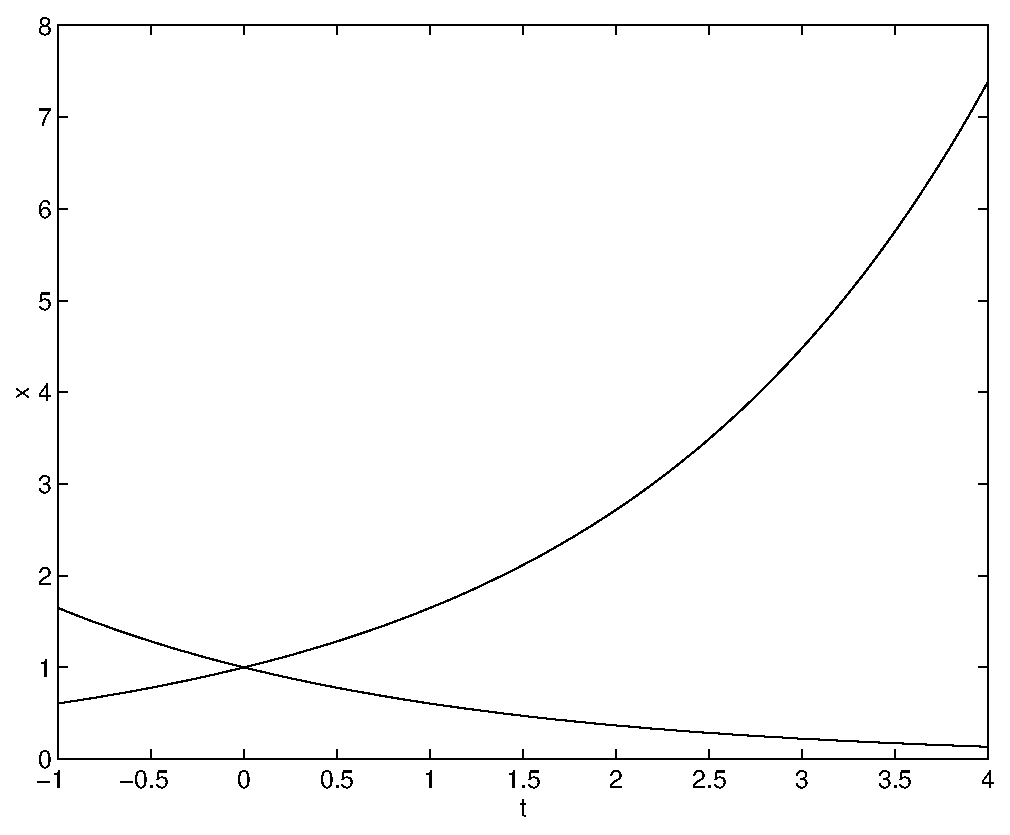
\psfig{file=figures/graph1.eps,width=3.5in}}
     \caption{Solutions of \protect\Ref{lin1}
              for $t\in [-1,4]$, $x_0=1$ and $\lambda=\pm 0.5$.}
     \label{graph_labelfig}
\end{figure}


  \subsubsection*{The Inhomogeneous Linear Differential Equation}

It follows from \Ref{explimits} that solutions to the linear homogeneous
differential equation \Ref{ivp1} are either unbounded as $t\to \infty$ or 
they approach zero.  Now we consider an inhomogeneous differential 
equation and show that solutions can approach fixed values for increasing 
$t$ that are neither zero nor infinity.

As an example, consider the linear differential equation
\begin{equation} \label{E:ivp2}
\frac{dx}{dt} = -2x-6.
\end{equation}
Observe that $x(t)=0$ is not a solution of \Ref{E:ivp2} and therefore
that \Ref{E:ivp2} is {\em inhomogeneous}.  It is easy to verify, however, 
that the constant function $x(t)=-3$ is a solution.

Equation~\Ref{E:ivp2} can be solved by introducing a new function that 
transforms \Ref{E:ivp2} into a homogeneous equation.  Let
\[
y(t) = x(t) + 3,
\]
and compute
\[
\frac{dy}{dt} = \frac{dx}{dt} = -2x-6 = -2y.
\]

Using Theorem~\ref{T:singleeqn}, it follows that $y(t)$ has the form
\[
y(t) = y_0e^{-2t}.
\]
Therefore
\[
x(t) =  y_0e^{-2t}-3
\]
is a solution of \Ref{E:ivp2} for every constant $y_0$.  Moreover, 
\[
\lim_{t\to\infty} x(t) = \lim_{t\to\infty} y_0e^{-2t} -3=-3,
\]
which is neither zero nor infinity.

Any equation of the form
\begin{equation} \label{ivp2}
\frac{dx}{dt}(t)  = \lambda x(t) +\rho
\end{equation}
can be solved in a similar fashion.  Just set 
\[
y(t) = x(t) + \frac{\rho}{\lambda}.
\]
It follows from \Ref{ivp2} that
\[
\frac{dy}{dt} = \frac{dx}{dt} = \lambda x(t) +\rho =
\lambda\left( y(t)-\frac{\rho}{\lambda}\right) +\rho = \lambda y(t).
\]
Theorem~\ref{T:singleeqn} implies that $y(t) = y_0e^{\lambda t}$ for some 
constant $y_0$ and
\[
x(t) = y_0e^{\lambda t} - \frac{\rho}{\lambda}.
\]
Note that the limit of $x(t)$ as $t\to\infty$ is $-\rho/\lambda$ when 
$\lambda<0$.



\subsection*{Some Examples of \protect\Ref{ivp1}}

Even though the differential equation \Ref{lin1} is one of the
simplest differential equations, it still has some use in applications.
We present two here: compound interest and population dynamics.

\subsubsection*{Compound Interest} \index{compound interest}

Banks pay interest on an account in the following way.  At the
end of each day, the bank determines the interest rate $r_{day}$ for
that day, checks the principal $P$ in the account, and then
deposits an additional $r_{day}P$.  So the next day the principal in
this account is $(1+r_{day})P$.  Note that if $r$ denotes the
interest rate per year, then $r_{day} = r/365$.  Of course, a day
is just a convenient measure for elapsed time.  Before computers
were prevalent, banks paid interest yearly or quarterly or monthly
or, in a few cases, even weekly, depending on the particular bank rules.

Observe that the more frequently interest is paid, the more
money is earned. For example, if interest is paid only once at
the end of a year, then the money in the account at the end of
the year is $(1+r)P$, and the amount $rP$ is called {\em simple
interest\/}.  But if interest is paid twice a year, then the principal
at the end of six months will be $(1+\frac{r}{2})P$, and the principal
at the end of the year will be $(1+\frac{r}{2})^2P$.  Since
\[
\left(1+\frac{r}{2}\right)^2 = 1+r+\frac{1}{4}r^2 > 1+r,
\]
there is more money in the account at the end of the
year if the interest is compounded semiannually rather than
annually.  But how much is the difference and what is the
maximum earning potential?

While making the calculation in the previous paragraph, we
implicitly made a number of simplifying assumptions.  In
particular, we assumed
\begin{itemize}
\item	an initial principal $P_0$ is deposited in the bank on January 1,
\item	the money is not withdrawn for one year,
\item	no new money is deposited in that account during the year,
\item	the yearly interest rate $r$ remains constant throughout
	the year, and
\item	interest is added to the account $N$ times during the year.
\end{itemize}
In this {\em model\/}, simple interest corresponds to $N=1$, compound monthly
interest to $N=12$, and compound daily interest to $N=365$.

We first answer the question: How much money is in this account after
one year?  After one time unit of $\frac{1}{N}$ year, the amount of
money in the account is
\[
Q_1 = \left(1+\frac{r}{N}\right)P_0.
\]
The interest rate in each time period is $\frac{r}{N}$,
the yearly rate $r$ divided by the number of time periods $N$.  Here
we have used the assumption that the interest rate remains constant
throughout the year.  After two time units, the principal is:
\[
Q_2 = \left(1+\frac{r}{N}\right)Q_1 = \left(1+\frac{r}{N}\right)^2P_0,
\]
and at the end of the year (that is, after $N$ time periods)
\begin{equation} \label{compint}
Q_N = \left(1+\frac{r}{N}\right)^N P_0.
\end{equation}
Here we have used the assumption that money is neither deposited nor
withdrawn from our account.   Note that $Q_N$ is the amount of money
in the bank after {\bf one} year assuming that interest has been
compounded $N$ (equally spaced) times during that year, and the effective
interest rate when compounding $N$ times is:
\[
\left(1+\frac{r}{N}\right)^N - 1.
\]

For the curious, we can write a program in \Matlab to compute
\Ref{compint}.  Suppose we assume that the initial deposit $P_0=\$1,000$,
the simple interest rate is $6\%$ per year, and the interest payments
are made monthly. In \Matlab type
\begin{verbatim}
N  = 12;
P0 = 1000;
r  = 0.06;
QN = (1 + r/N)^N*P0
\end{verbatim}
The answer is $QN=\$1,061.68$, and the {\em effective\/}
interest rate for monthly payments is $6.16778\%$.  For daily
interest payments $N=365$, the answer is $QN=\$1,061.83$, and
the effective interest rate is $6.18313\%$.

To find the maximum effective interest, we ask the bank to compound interest
continuously; that is, we ask the bank to compute
\[
\lim_{N\to\infty} \left(1 + \frac{r}{N}\right)^N.
\]
We compute this limit using differential equations.  The concept of
continuous interest is rephrased as follows.  Let $P(t)$ be the
principal at time $t$, where $t$ is measured in units of years.
Suppose that we assume that interest is compounded $N$ times during
the year.  The length of time in each compounding period is
\[
\Delta t = \frac{1}{N},
\]
and the change in principal during that time period is
\[
\Delta P = \frac{r}{N} P = rP\Delta t.
\]
It follows that
\[
\frac{\Delta P}{\Delta t} = rP,
\]
and, on taking the limit $\Delta t \to 0$, we have the differential equation
\[
\frac{dP}{dt}(t) = rP(t).
\]

Since $P(0)=P_0$ the solution of the initial value problem given
in Theorem~\ref{T:singleeqn} shows that
\[
P(t) = P_0 e^{rt}.
\]
After one year ($t=1$) we find that
\[
P(1) =  e^r P_0.
\]
Note that
\[
P(1) = \lim_{N\to\infty} Q_N,
\]
and we have thus verified that
\[
 \lim_{N\to\infty} \left(1 + \frac{r}{N}\right)^N = e^r.
\]
Thus the maximum effective interest rate is $e^r-1$.  When $r=6\%$
the maximum effective interest rate is $6.18365\%$.


\subsubsection*{An Example from Population Dynamics}
\index{population dynamics}

To provide a second interpretation of the constant $\lambda$ in
\Ref{lin1}, we discuss a simplified model for population dynamics.
Let $p(t)$ be the size of a population of a certain species at
time $t$ and let $r$ be the rate at which the population $p$ is
changing at time $t$.  In general, $r$ depends on the time $t$
and is a complicated function of birth and death rates and of
immigration and emigration, as well as of other factors.
Indeed, the rate $r$ may well depend
on the size of the population itself.  (Overcrowding can be
modeled by assuming that the death rate increases with the size
of the population.) These population models assume that the
rate of change in the size of the population $dp/dt$ is given by
\begin{equation}  \label{pop_model}
        \frac{dp}{dt}(t) = r p(t),
\end{equation}
they just differ on the precise form of $r$.  In general, the
rate $r$ will depend on the size of the population $p$ as well
as the time $t$, that is, $r$ is a function $r(p,t)$.

The simplest population model\index{population model} --- which
we now assume --- is the
one in which $r$ is assumed to be constant.  Then equation
\Ref{pop_model} is identical to \Ref{lin1} after identifying $p$
with $x$ and $r$ with $\lambda$.  Hence we may interpret $r$ as
the growth rate for the population.  The form of the solution in
\Ref{soln1} shows that the size of a population grows
exponentially if $r>0$ and decays exponentially if $r<0$.

The mathematical description of this simplest population model
shows that the assumption of a constant growth rate leads to
exponential growth (or exponential decay).  Is this realistic?
Surely, no population will grow exponentially for all time, and
other factors, such as limited living space, have to be taken
into account.  On the other hand, exponential growth describes
well the growth in human population during much of human
history.  So this model, though surely oversimplified, gives
some insight into population growth.

\EXER

\TEXER


\noindent In Exercises~\ref{c3.1.a01a} -- \ref{c3.1.a01c} find
solutions to the given initial value problems.
\begin{exercise} \label{c3.1.a01a}
$\frac{\dps dx}{\dps dt} = \sin(2t),\quad x(\pi) = 2$.
\end{exercise}
\begin{exercise} \label{c3.1.a01b}
$\frac{\dps dx}{\dps dt} = t^2, \quad x(2) = 8$.
\end{exercise}
\begin{exercise} \label{c3.1.a01c}
$\frac{\dps dx}{\dps dt} = \frac{1}{t^2},\quad x(1)=1$.
\end{exercise}

\noindent In Exercises~\ref{c3.1.ba} -- \ref{c3.1.bd} determine whether
or not each of the given functions $x_1(t)$ and $x_2(t)$ is a solution 
to the given differential equation.
\begin{exercise}  \label{c3.1.ba}
ODE:\quad $\frac{\dps dx}{\dps dt} = \frac{\dps t}{\dps x-1}$.
Functions:\quad $x_1(t)=t+1 \AND x_2(t)= \frac{\dps 1+\sqrt{4t^2+1}}{\dps 2}$.
\end{exercise}
\begin{exercise}  \label{c3.1.bb}
ODE:\quad $\frac{\dps dx}{\dps dt} = x + e^t$.
Functions:\quad $x_1(t)=te^t \AND x_2(t)= 2e^t$.
\end{exercise}
\begin{exercise}  \label{c3.1.bc}
ODE:\quad $\frac{\dps dx}{\dps dt} = x^2 + 1$.
Functions:\quad $x_1(t)=-\tan t \AND x_2(t)= \tan t$.
\end{exercise}
\begin{exercise}  \label{c3.1.bd}
ODE:\quad $\frac{\dps dx}{\dps dt} = \frac{\dps x}{\dps t}$.
Functions:\quad $x_1(t)=t+1 \AND x_2(t)= 5t$.
\end{exercise}


\begin{exercise} \label{c3.1.1}
Solve the differential equation
\[
\frac{dx}{dt} = 2x,
\]
where $x(0)=1$.  At what time $t_1$ will $x(t_1)=2$?
\end{exercise}

\begin{exercise} \label{c3.1.2}
Solve the differential equation
\[
\frac{dx}{dt} = -3x.
\]
At what time $t_1$ will $x(t_1)$ be half of $x(0)$?
\end{exercise}

\begin{exercise} \label{c3.1.3}
Bacteria grown in a culture increase at a rate proportional to the
number present.  If the number of bacteria doubles every $2$ hours,
then how many bacteria will be pre\-sent af\-ter $5$ hours?  Express
your answer in terms of $x_0$, the initial number of bacteria.
\end{exercise}

\begin{exercise} \label{c3.1.4}
Suppose you deposit \$10,000 in a bank at an
interest of $7.5\%$ compounded continuously.
How much money will be in your account a year and a half later?
How much would you have if the interest were compounded monthly?
\end{exercise}

\begin{exercise} \label{c3.1.5} \index{Newton's law of cooling}
Newton's law of cooling states that the rate at which a body changes
temperature is proportional to the difference between the body
temperature and the temperature of the surrounding medium.  That is,
\begin{equation}  \label{e:Newton}
\frac{dT}{dt} = \alpha(T-T_m)
\end{equation}
where $T(t)$ is the temperature of the body at time $t$, $T_m$ is the
constant temperature of the surrounding medium, and $\alpha$ is the
constant of proportionality.  Suppose the
body is in air of temperature $50^\circ$ and the body cools from
$100^\circ$ to $75^\circ$ in $20$ minutes.  What will the temperature
of the body be after one hour?  {\bf Hint:} Rewrite \Ref{e:Newton} in
terms of $U(t) = T(t) - T_m$.
\end{exercise}

\begin{exercise} \label{c3.1.6}
\index{population dynamics}
Let $p(t)$ be the population of group Grk at time $t$ measured in years.
Let $r$ be the growth rate of the group Grk.  Suppose that the population
of Grks changes according to the differential equation \Ref{pop_model}.
Find $r$ so that the population of Grks doubles every $50$ years.  How
large must $r$ be so that the population doubles every $25$ years?
\end{exercise}

\begin{exercise} \label{c3.1.7A}
You deposit \$4,000 in a bank at an interest of $5.5\%$ but after half 
a year the bank changes the interest rate to $4.5\%$.  Suppose that the 
interest is compounded continuously.  How much money will be in your 
account after one year?
\end{exercise}

\begin{exercise} \label{c3.1.7}
As an application of \Ref{e:intcalcsoln} answer the following question
(posed by R.P. Agnew).
\begin{quote}
One day it started snowing at a steady rate.  A snowplow started at
noon and went two miles in the first hour and one mile in the second
hour.  Assume that the speed of the snowplow times the depth of the
snow is constant.  At what time did it start to snow?
\end{quote}

\noindent To set up this problem, let $d(t)$ be the depth of the snow
at time $t$ where $t$ is measured in hours and $t=0$ is noon.
Since the snow is falling at a constant rate $r$, $d(t)= r(t-t_0)$
where $t_0$ is the time that it started snowing.  Let $x(t)$ be the
position of the snowplow along the road.  The assumption that speed
times the depth equals a constant $k$ means that
\[
\frac{dx}{dt}(t) = \frac{k}{d(t)} = \frac{K}{t-t_0}
\]
where $K=k/r$.  The information about how far the snowplow goes in the
first two hours translates to
\[
x(1) = 2  \AND x(2) =3.
\]
Now solve the problem.
\end{exercise}


\CEXER

\noindent In Exercises~\ref{c3.1.a78a} -- \ref{c3.1.a78d} use \Matlab
to graph the given function $f$ on the specified interval.
\begin{exercise} \label{c3.1.a78a}
$f(t) = t^2$ on the interval $t\in [0,2]$.
\end{exercise}
\begin{exercise} \label{c3.1.a78b}
$f(t) = e^t-t$ on the interval $t\in [0,3]$.
\end{exercise}
\begin{exercise} \label{c3.1.a78c}
$f(t) = \cos(2t)-t$ on the interval $t\in [2,8]$.
\end{exercise}
\begin{exercise} \label{c3.1.a78d}
$f(t) = \sin(5t)$ on the interval $t\in [0,6.5]$.
\end{exercise}

\noindent{\bf Hint:} Use the fact that the trigonometric functions $\sin$ and
$\cos$ can be evaluated in \Matlab in the same way as the exponential
function, that is, by using \verb+ sin + \index{\computer!sin} and
\verb+ cos + \index{\computer!cos} instead of \verb+ exp+.

\begin{exercise} \label{c3.1.8}
Two banks each pay $7\%$ interest per year --- one compounds money
daily and one compounds money continuously.  What is the difference
in earnings in one year in an account having \$10,000.
\end{exercise}

\begin{exercise} \label{c3.1.9}
There are two banks in town --- Intrastate and Statewide.  You plan
to deposit \$5,000 in one of these banks for two years.  Statewide Bank's
best savings account pays $8\%$ interest per year compounded quarterly
and charges \$10 to open an account.  Intrastate Bank's best savings
account pays $7.75\%$ interest compounded daily.  Which bank will
pay you the most money when you withdraw your money?  Would your
answer change if you had planned to keep your money in the bank
for only one year?
\end{exercise}

\begin{exercise} \label{c3.1.10}
In the beginning of the year 1990 the population of the United States was
approximately 250,000,000 people and the growth rate was estimated at $3\%$
per year.  Assuming that the growth rate does not change, during what year
will the population of the United States reach 400,000,000?
\end{exercise}


\section{Graphing Solutions to Differential Equations}
\label{S:3.2}

Solutions to differential equations can be graphed in several
different ways, each giving different insight into the structure
of the solutions.  We begin by asking what object is to be
graphed.  Do we first solve the differential equation and then
graph the solution, or do we let the computer find the solution
numerically and then graph the result?  The first method assumes
that we can find a formula for the solution (such as
$x(t)=x_0e^{\lambda t}$).  A solution to a differential equation
for which we have an explicit formula is called a {\em closed
form\/} solution\index{closed form solution}.  Using \Matlab we
can graph closed form solutions, as we showed in
Figure~\ref{graph_labelfig}. The second method of graphing
solutions requires having a numerical method that can {\em
numerically integrate\/} the differential equation to any
desired degree of accuracy.

In fact, there are rather few differential equations that can be
solved in closed form (though the linear systems that we
describe in this chapter are ones that can be solved in closed
form).  Without formulas, the first method is impossible.  There
are, however, several efficient algorithms for the numerical
solution of (systems of) ordinary differential equations and
these methods have been preprogrammed in \Matlabp.  In our
discussions, we treat \Matlab as a {\em black box\/} numerical
integration solver of ordinary differential equations.

\subsection*{A Single First Order Ordinary Differential Equation}

We begin our discussion of the numerical integration of
differential equations with the single first order \index{first
order}\index{differential equation!first order} differential equation
of the form:
\begin{equation} \label{nonaut}
\frac{dx}{dt}(t) = f(t,x(t)).
\end{equation}
The equation is {\em first order\/} since only the first
derivative of the function $x(t)$ appears in the equation. If
the second derivative appeared in the equation, then the equation
would be a second order equation.

\subsubsection*{Independent ($t$) and Dependent ($x$) Variables}

Sometimes this equation is also written in the form
\begin{equation}  \label{nonaut2}
	\frac{dx}{dt} = f(t,x)
\end{equation}
and in this form both $t$ and $x$ appear as variables.  But $x$
is a function $x(t)$ depending on $t$, and therefore the
variable $t$ is called the {\em independent\/}
\index{independent variable} variable, while the variable $x$ is
called the {\em dependent\/} \index{dependent variable} variable.

\subsubsection*{Autonomous versus Nonautonomous}

When the right hand side $f$ does not depend explicitly on the
independent time variable $t$, then the equation is called {\em
autonomous\/}\index{autonomous}\index{differential equation!autonomous}.
More explicitly, in
\Ref{nonaut2}, the differential equation is autonomous when
$f(t,x)=g(x)$.  Equation \Ref{lin1} is an example of an
autonomous differential equation since $f(t,x)=\lambda x$.

When $f$ depends explicitly on the independent time variable $t$,
the differential equation is called {\em nonautonomous\/}.
\index{nonautonomous}\index{differential equation!nonautonomous}
Suppose in our example of interest rates  in Section~\ref{S:growthmodels}
we had assumed that the interest rate $r$ changes in time.  In
such a case we would write $r=r(t)$ and the differential equation modeling 
how the principal $P(t)$ changes in time would be written as
\begin{equation}  \label{E:varinterest}
\frac{dP}{dt} = r(t)P.
\end{equation}
This equation is an example of a nonautonomous differential equation 
since $f(t,P) = r(t)P$.   For instance, suppose that at time $t=0$ the
principal in our account is $P_0$, and the interest rate is $5.5\%$.  
Now suppose the bank changes the interest rate after six months to $4.5\%$. 
Then $P(t)$ is a solution to \Ref{E:varinterest}, where
\[
  r(t) = \left\{\begin{array}{l}
     0.055\quad\mbox{for $0\le t < 0.5$, and}\\
     0.045\quad\mbox{for $0.5\le t$,}
  \end{array}\right.
\]
and $P(0)=P_0$.

Another example of a nonautonomous differential equation is given by
\begin{equation}  \label{dfeq}
\frac{dx}{dt} = x^2-t.
\end{equation}


\subsection*{Time Series and Phase Space Plots}

There are two different methods for visualizing the result of
numerical integration of differential equations of the form
\Ref{nonaut}: time series plots and phase space plots.  These
two methods are based on interpreting the derivative $dx/dt$
alternatively as either the slope of a tangent line or as the
velocity of a particle.

A {\em time series\/} \index{time series} plot for a solution to
\Ref{nonaut} is found by plotting $x$ versus $t$ as we did for
the closed form solution in Figure~\ref{graph_labelfig}.  However,
when graphing time series of solutions we do not need to find closed
form solutions.  To understand how this is done, we briefly discuss
what equation \Ref{nonaut} is actually saying about a solution
$x(t)$.  This equation states that the slope of the tangent line
to the graph of the function $x(t)$ at time t ($dx/dt$) is known
and equals $f(t,x(t))$.  Thus we can use the right hand side of
\Ref{nonaut} to draw the tangent lines to $x(t)$ at each point
in the $tx$-plane.  This leads to the notion of a line field.
The rough idea behind the numerical integration scheme is to fit
a curve $(t,x(t))$ into the $tx$-plane in such a way that the
tangent lines to the curve match the tangent lines specified by
the slope $f$.

A {\em phase space\/} \index{phase!space} plot is based on
the {\em other\/} interpretation of a derivative as a rate of
change --- a velocity.  We let $x(t)$ denote the position of a
particle on the real line at time $t$.  The function $f(t,x)$
denotes the velocity of that particle when the particle is at
position $x$ at time $t$.  Thus, to view the phase space plot,
we need to see the particle moving along the real line; that is,
we need to see how $x(t)$ changes in $t$.  Later, we will use
\Matlab graphics to actually visualize the particle movement.

Thus time series are graphs of functions in the $tx$-plane while
phase space plots are graphs on the real line $x$.  We discuss
time series plots in this section and phase line plots in the
next.


\subsection*{Line Fields}

We begin our discussion of line fields \index{line field} (or
synonymously direction fields) \index{direction field} by
focusing on the information about solutions that can directly
be extracted from the equation itself.  To illustrate this we
consider the differential equation \Ref{dfeq}.

As mentioned, the differential equation $\dot{x}=x^2-t$ reflects the fact 
that the value of the derivative of a solution $x(t)$ at time $t$ is
given by $(x(t))^2-t$.  In other words, the slope of the tangent
line to the solution is known and is given by the right hand
side of the differential equation.

We can use this information to sketch all the tangent lines at
each point $(t_0,x_0)$ of a rectangle in the $tx$-plane.  We do
this by drawing a small line segment at each point with the
slope determined by the right hand side.  In this way we obtain the
{\em line field}.  In Figure~\ref{df1_labelfig} we show a
line field corresponding to the differential equation \Ref{dfeq}.

\begin{figure}[htb]
        \centerline{%
        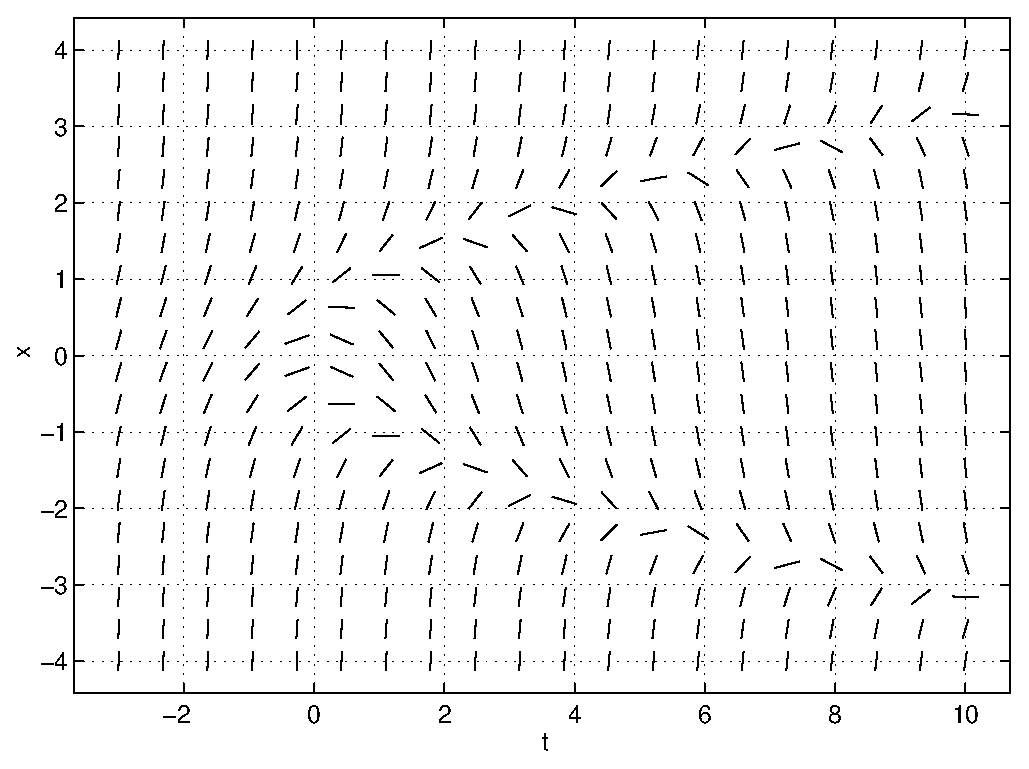
\psfig{file=figures/df1.eps,width=3.0in}
	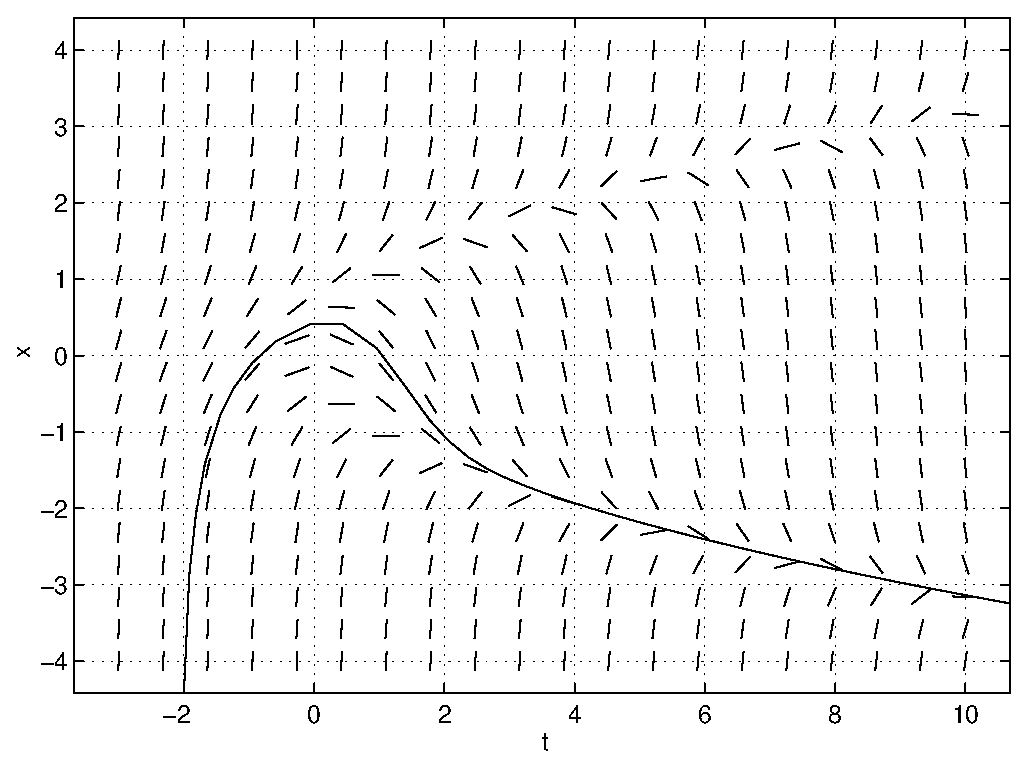
\psfig{file=figures/df3.eps,width=3.0in}}
        \caption{Left: Line field for \protect\Ref{dfeq}
              for $t\in [-3,10]$ and $x\in [-4,4]$.
	      Right: a solution starting for $t=-2$ at $x(-2)=-4$.}
        \label{df1_labelfig}
\end{figure}

By looking at the left hand image in Figure~\ref{df1_labelfig}
we can imagine how solution curves fit into the diagram; indeed,
we can almost use this line field to make freehand sketches
of solutions to \Ref{dfeq}.  The right hand image in
Figure~\ref{df1_labelfig} shows the solution starting at the
initial condition $x(-2) = -4$, which is the point $(x,t)=(-4,-2)$.


\subsection*{Graphing Solutions Using {\sf dfield5}}
\index{\computer!dfield5}

We now explain how to use \Matlab to display the graphs of
solutions to the differential equation \Ref{dfeq} for different
choices of initial conditions.  It is a tedious process to use
\Matlab directly to both compute and graphically display these
solutions.  Instead, we use a program written in \Matlab by John
Polking\index{Polking, John} for graphing both the line field and the time 
series of a solution to any ordinary differential equation of the form
\Ref{nonaut}.  In \Matlab this program is addressed by typing
\begin{verbatim}
dfield5
\end{verbatim}
In response, a window appears with the title {\sf
DFIELD5 Setup.}  The differential equation under consideration is 
displayed in the upper big grey frame.  In this case it is
\[
	x' = x^2 - t,
\]
which is \Ref{dfeq}.  Now use the left 
mouse button to click onto the button {\sf Proceed}.  
Then another window, having the title {\sf DFIELD5 Display},
appears.  In this window, one should see the line
field shown in Figure~\ref{df1_labelfig}.  We may compute the
solution going through the point $(t_0,x_0)=(-2,-4)$ in the
$(t,x)$-plane by clicking on that point with any mouse button.
{\sf dfield5} should reproduce the right hand side in
Figure~\ref{df1_labelfig}.

Suppose that we want to solve numerically equation \Ref{lin1}
using {\sf dfield5}. To enter this equation with $\lambda = 0.5$,
we have to change the setup.  Begin by clicking into the window
where the right hand side {\sf x\^{$\,\!$}2--t} can be found and
then replace it by {\sf 0.5*x}.  Now use the left mouse button
to click onto the button {\sf Proceed}.  In the window titled
{\sf DFIELD5 Display}, one should see the line field
\index{line field!in {\sf dfield5}} shown on
the left in Figure~\ref{df_dsp1}.
\begin{figure}[htb]
    \centerline{%
    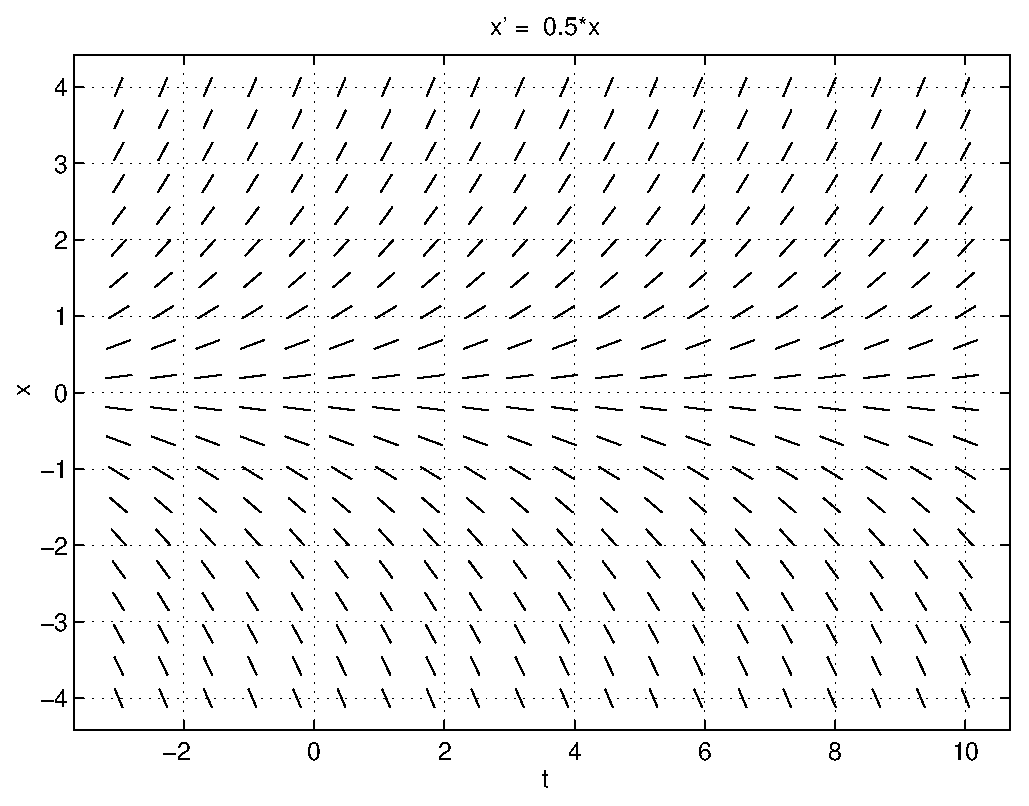
\psfig{file=figures/df_dsp1.eps,width=3.0in}
    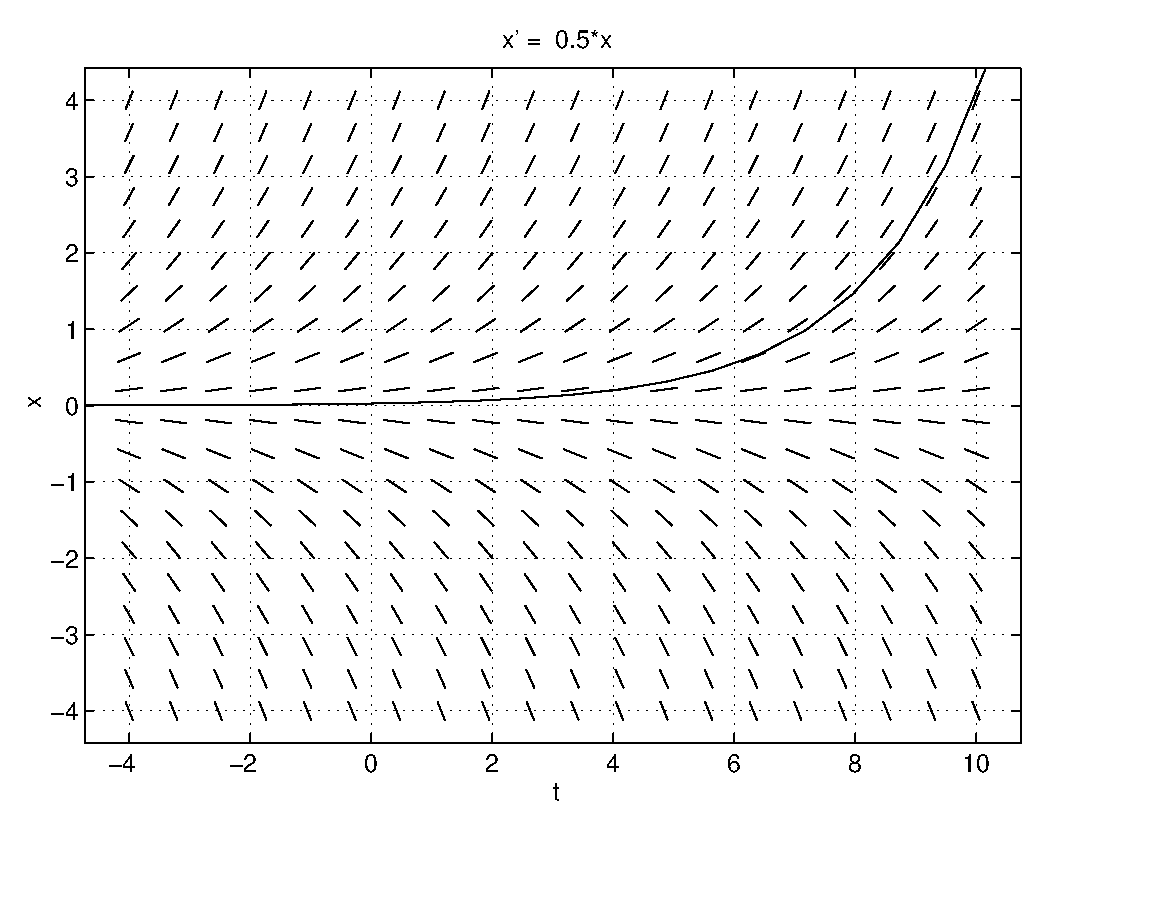
\psfig{file=figures/dfr_dsp1.eps,width=3.0in}}
    \caption{Left: Line field for $\dot{x}=0.5x$ for $t\in [-4,10]$ and
		$x\in [-4,4]$.  Right: A solution starting at $t=0$ and
		$x>0$ but small.}
    \label{df_dsp1}
\end{figure}

Now we may compute solutions going through a certain point
$(t_0,x_0)$ in the $(t,x)$-plane by clicking with any mouse
button on that point.  The solution is then computed first in
forward time and then in backward time.  For example, if we
click on a point near $t=x=0$ where $x>0$, {\sf dfield5} produces
the solution shown on the right in Figure~\ref{df_dsp1}.  Note
the similarity with the graph of the closed form solution in
Figure~\ref{graph_labelfig} when $\lambda=0.5$.

By clicking several times it appears that all solutions diverge
to either plus or minus infinity as $t$ goes to infinity.
Indeed, by \Ref{soln1} we know that the solutions are of the
form $x(t) = x_0 e^{0.5 t}$, and hence this behavior is expected
for $x_0\not= 0$.  To compute a solution corresponding to the case
when $x_0=0$, we bring up the menu {\sf DFIELD5 Options} and select
{\sf Keyboard input}.  This allows us to type in the initial
values $t=-2$ and $x=0$.  The action {\sf Compute} then leads to
the computation of the solution $x(t)=0$ corresponding to $x_0=0$.

The value of $\lambda=0.5$ can be changed by editing the
corresponding window in the {\sf DFIELD5 Setup.} For instance, if
we replace the $0.5$ by $-0.8$ and push {\sf Proceed}, then the
current line field is replaced by the line field shown
in Figure~\ref{df_dsp2}.
\begin{figure}[htb]
    \centerline{%
    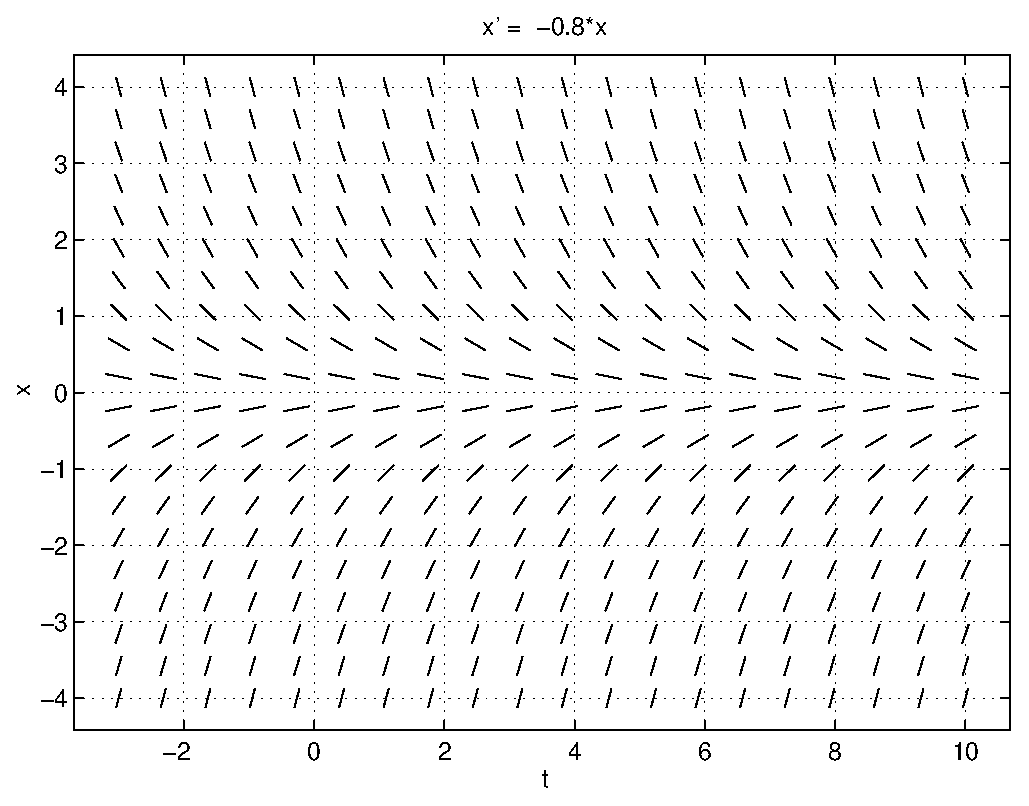
\psfig{file=figures/df_dsp2.eps,width=3.0in}
    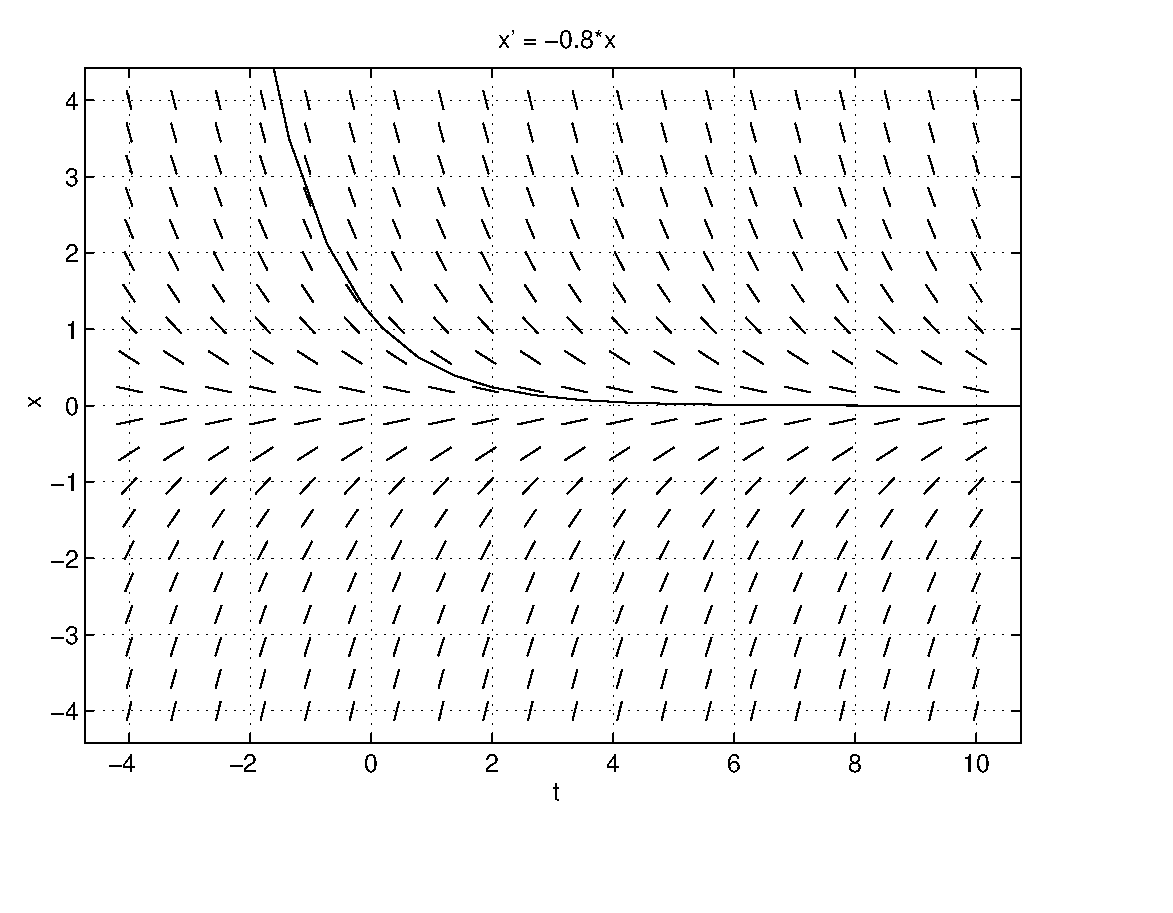
\psfig{file=figures/dfr_dsp2.eps,width=3.0in}}
    \caption{Left: Line field for $\dot{x}=-0.8 x$ for $t\in [-4,10]$
	and $x\in [-4,4]$.  Right: A solution starting at $t=0$ and
	$x$ between $1$ and $2$.}
    \label{df_dsp2}
\end{figure}

By computing different solutions, it seems as though all of them
converge to zero as $t$ goes to infinity, which agrees with
\Ref{explimits}.


\subsubsection*{Autonomous and Nonautonomous Equations in {\sf dfield5}}

In a sense, solutions of autonomous equations do not depend on the initial
time $t_0$, but just on the initial position $x_0$.  More precisely, let
$x_1(t)$ be the solution to
\[
\frac{dx}{dt} = f(x)
\]
with initial condition $x(0)=x_0$ and let $x_2(t)$ be a solution
to the same differential equation with initial condition $x(t_0)=x_0$.
Then
\begin{equation}  \label{E:initdiff}
x_2(t) = x_1(t-t_0).
\end{equation}
This statement can be verified by noting that the definition of
$x_2(t)$ in \Ref{E:initdiff} satisfies the initial value
\[
x_2(t_0)=x_1(t_0-t_0)=x_1(0)=x_0,
\]
and, using the chain rule, the differential equation
\[
\frac{dx_2}{dt}(t) = \frac{dx_1}{dt}(t-t_0) = f(x_1(t-t_0))=f(x_2(t)).
\]
So the solution $x_2(t)$ is the same as the solution $x_1(t)$ with
just a shift in time $t$.  In general, the same statement is {\em not\/} 
true for nonautonomous equations.

This difference between autonomous and nonautonomous equations can be
visualized using {\sf dfield5}. On the left in Figure~\ref{F:non-auto}
we graph two solutions of the {\em autonomous\/} differential equation
$\dot{x}=x^2-2x$ with initial conditions $x(0)=1$ and $x(2)=1$.  Note
that one solution is obtained from the other just by shifting by two
time units.  On the right of that figure we graph two solutions of the
{\em nonautonomous\/} differential equation $\dot{x}=x^2-t$ with
initial conditions $x(0)=1$ and $x(2)=1$.  Note that the two solutions
are most definitely not obtained one from the other by a time shift.

\begin{figure}[htb]
        \centerline{%
        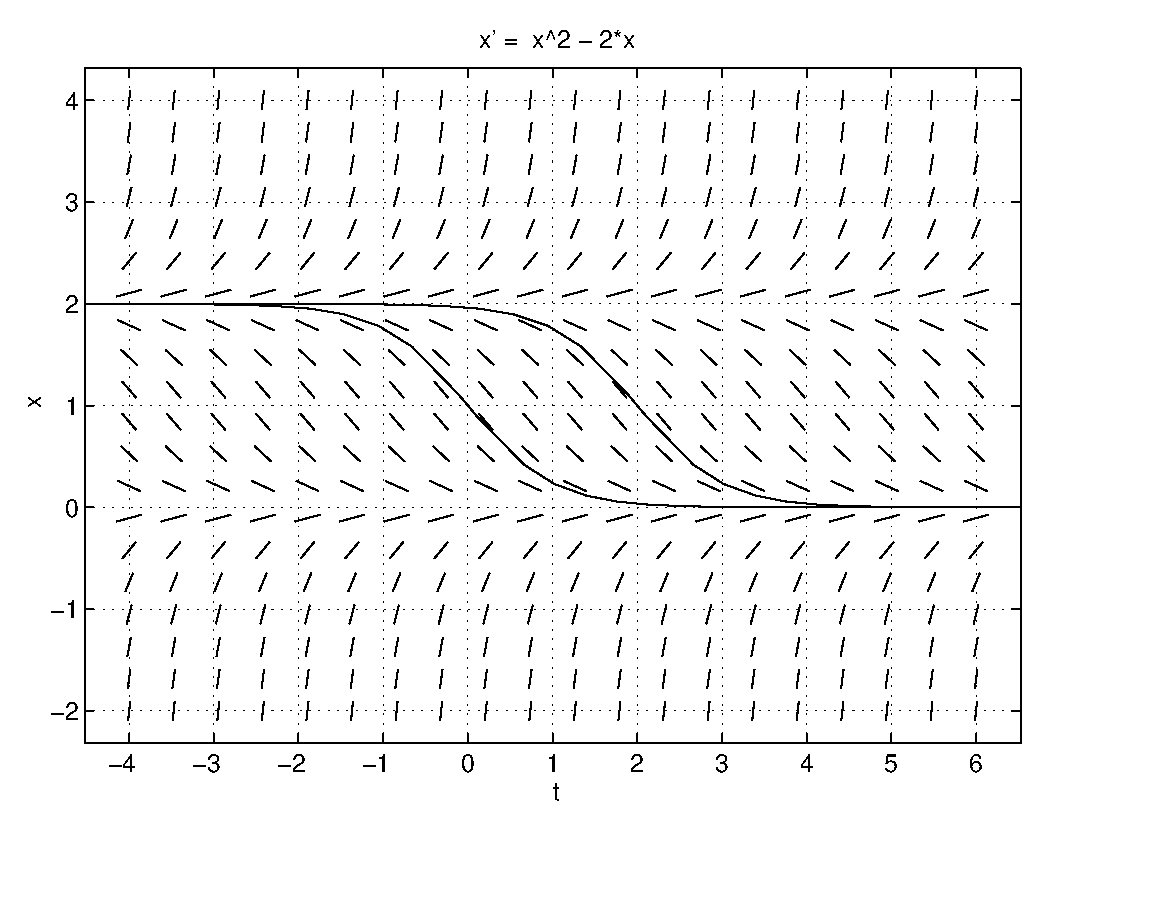
\psfig{file=figures/auto.eps,width=3.0in}
	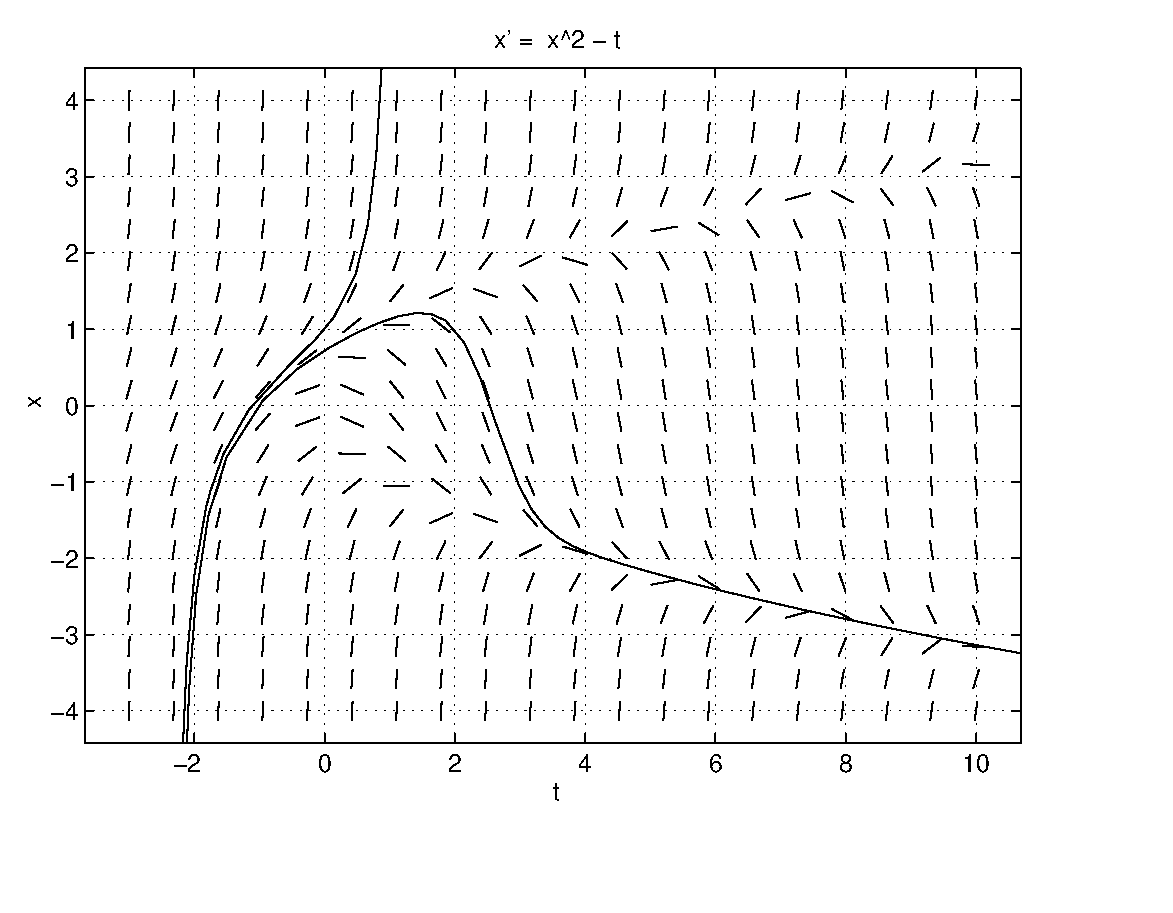
\psfig{file=figures/nonauto.eps,width=3.0in}}
        \caption{Left: Solutions of the autonomous equation $\dot{x}=x^2-2x$
	with initial conditions $x(0)=1$ and $x(2)=1$. Right: Solution of
	the nonautonomous differential equation $\dot{x}=x^2-t$ with initial
	conditions $x(0)=1$ and $x(2)=1$.}
        \label{F:non-auto}
\end{figure}


\EXER

\TEXER

\noindent In Exercises~\ref{c3.2.1A} -- \ref{c3.2.1D} determine whether the 
solution to the given differential equation with given initial condition is 
increasing or decreasing at the initial point.
\begin{exercise} \label{c3.2.1A}
ODE: $\dot{x}=x-t$; initial condition: $x(1)=2$.
\end{exercise}
\begin{exercise} \label{c3.2.1B}
ODE: $\dot{x}=x-t$; initial condition: $x(2)=1$.
\end{exercise}
\begin{exercise} \label{c3.2.1C}
ODE: $\dot{x}=x^2-tx$; initial condition: $x(1)=2$.
\end{exercise}
\begin{exercise} \label{c3.2.1D}
ODE: $\dot{x}=x^2-tx-t$; initial condition: $x(2)=-1$.
\end{exercise}

\noindent In Exercises~\ref{c3.2.2A} -- \ref{c3.2.2D} sketch by hand the line 
field of the given differential equation on the given rectangle.
\begin{exercise} \label{c3.2.2A}
ODE: $\dot{x}=x-t$; rectangle: $0\leq x\leq 2; -1\leq t\leq 1$.
\end{exercise}
\begin{exercise} \label{c3.2.2B}
ODE: $\dot{x}=x+t$; rectangle: $-2\leq x\leq 2; -1\leq t\leq 2$.
\end{exercise}
\begin{exercise} \label{c3.2.2C}
ODE: $\dot{x}=xt$; rectangle: $-1\leq x\leq 1; -1\leq t\leq 1$.
\end{exercise}
\begin{exercise} \label{c3.2.2D}
ODE: $\dot{x}=x/t$; rectangle: $0< x\leq 2; 0< t\leq 2$.
\end{exercise}

\noindent In Exercises~\ref{c3.2.3A} -- \ref{c3.2.3D} determine whether the 
given differential equation is autonomous or nonautonomous.
\begin{exercise} \label{c3.2.3A}
$\dot{x}=x-t$.
\end{exercise}
\begin{exercise} \label{c3.2.3B}
$\dot{x}=x^2-x$.
\end{exercise}
\begin{exercise} \label{c3.2.3C}
$\dot{x}=x\sin(x)$.
\end{exercise}
\begin{exercise} \label{c3.2.3D}
$\dot{x}=x\cos(t)$.
\end{exercise}


\CEXER

\noindent In Exercises~\ref{c3.2.a01a} -- \ref{c3.2.a01c} use
{\sf dfield5} to compute several solutions to the given differential
equations in the specified region.
\begin{exercise} \label{c3.2.a01a}
$\dot{x} = xt$, $t\in[0,2]$, $x\in[-1,1]$.
\end{exercise}
\begin{exercise} \label{c3.2.a01b}
$\dot{x} = tx^2$, $t\in[0,4]$, $x\in[-4,4]$.
\end{exercise}
\begin{exercise} \label{c3.2.a01c}
$\dot{x} = x-\sin(t)$, $t\in[-2,10]$, $x\in[-4,4]$.
\end{exercise}

\begin{exercise} \label{c3.2.1*}
Compute $x(2)$, where $x(t)$ is the solution to the differential equation 
$\dot{x} = 0.6x$ with initial condition $x(0)=0.5$, in two different ways, 
as follows:
\begin{itemize}
\item[(a)] Use {\sf Keyboard input} in {\sf dfield5} to compute the 
solution with initial value $x(0)=0.5$.  Use the {\sf zoom in} feature in 
the {\sf DFIELD5 Edit} menu to compute $x(2)$ to an accuracy of two decimal 
places.  (Drag a rectangle around the point you are interested in.  Repeat 
this several times until you can read off the value $x(2)$ of the solution.)  
\item[(b)] Use \Matlab to compute the value of the exact solution
of the form \Ref{soln1} with initial value $x(0)=0.5$.  
\item[(c)] Is your answer obtained using {\sf dfield5} in (a) accurate to 
within two decimal places of the answer obtained using (b)?  If not, 
which answer do you trust more, and why?
\end{itemize}
\end{exercise}

\begin{exercise} \label{c3.2.2}
Use {\sf dfield5} to compute solutions to the differential equation
$\dot{x} = x^2-tx+2t$. Use {\sf Keyboard input} to compute the solution
with initial value $x(-1)=-1$.  What is the minimum value of this
solution $x(t)$ on the interval $-2\leq t\leq 1$?  Plot
solutions to this equation starting with at least six or seven
different initial conditions. Then print the result.
\end{exercise}

\begin{exercise} \label{c3.2.3}
Use {\sf dfield5} to compute solutions to the differential
equation
\begin{equation}  \label{E:freehand}
\dot{x} = x^3-2t^2x-t.
\end{equation}
Print the line field of \Ref{E:freehand} on the intervals
$t\in[-2,2]$ and $x\in[-2,3]$.  Use the line field to draw freehand
the solution to \Ref{E:freehand} starting at $(t_0,x_0)=(-2,1)$.
Then set the initial condition using {\sf Keyboard input}
and print the numerically computed solution. Finally, compare
your freehand drawing with the numerically computed result.
\end{exercise}

\begin{exercise}  \label{exer:at}
\begin{itemize}
\item[(a)]  Draw the direction field for
\begin{equation} \label{ex:at}
\frac{dx}{dt} = \frac{x}{x-t}.
\end{equation}
Assuming that $x(2)=3$, estimate $x(137)$.
\item[(b)]  Verify that
\[
x(t) = t + \sqrt{t^2-3}
\]
is the solution to \Ref{ex:at}.  Then show that $x(t)$ satisfies the
initial condition $x(2)=3$.
\item[(c)]  Compare your estimate of the solution to \Ref{ex:at}
obtained using {\sf dfield5} with the exact solution
\[
x(137)= 137 +\sqrt{18766} \approx 273.989
\]
\end{itemize}
\end{exercise}

\section{Phase Space Pictures and Equilibria} \label{S:PSP&E}

Recall that in a {\em phase space\/} \index{phase!space} plot, the 
solution $x(t)$ represents the position $x$ of a particle on a line 
for each time $t$.  Phase space plots are difficult to draw, since 
motion must be built into the plot.  However, we can view this 
dynamically in \Matlab using the program {\sf pline}. \index{\computer!pline}

In this discussion, we will only plot solutions of autonomous,
first order differential equations; that is, equations of the
form
\[
\dot{x} = g(x).
\]
To begin, type
\begin{verbatim}
pline
\end{verbatim}
and the window with the {\sf PLINE Setup} appears on the
computer screen.  The layout is essentially the same as in the
{\sf DFIELD5 Setup} described above.  However, there are two
differences:
\begin{enumerate}
\item Since we assume that our equation is autonomous, the time
variable --- the independent variable --- does
not appear explicitly and no time interval is specified.  Rather
the {\sf Integration time}, the period for which the solution is
to be computed, has to be declared.  This change is due to the
convention that all numerical computations start at $t=0$.
\item We may enter equations with one free parameter.
In the {\sf PLINE Setup} that parameter is {\sf lambda}.
Moreover, we may choose the value for that parameter.  The
default value in the {\sf PLINE Setup} is $-0.8$.  Hence, the
default equation used by {\sf pline} is equation
\Ref{lin1} with $\lambda = -0.8$.
\end{enumerate}

When we click with the left mouse button onto the button {\sf
Proceed}, then the display window with the title {\sf PLINE
Display} opens and the $x$-axis shown in Figure~\ref{pl_dsp1}
becomes visible.

\begin{figure}[htb]
     \centerline{%
     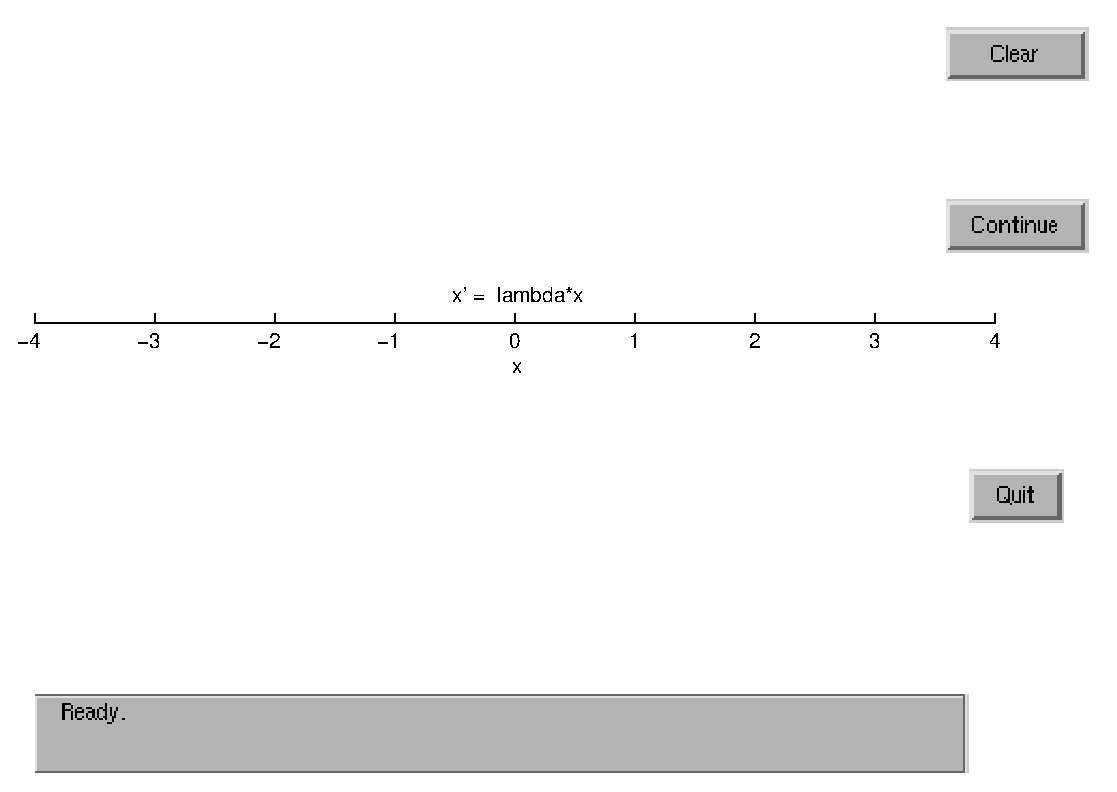
\psfig{file=figures/pl_dsp1.eps,height=2.6in}}
     \caption{{\sf PLINE Display} for $\dot{x}=\lambda x$
                and $x\in [-4,4]$.}
     \label{pl_dsp1}
\end{figure}

Similar to {\sf dfield5} we may start the numerical solution by
clicking with the left mouse button on the initial value of $x$.
It is not necessary to hit the axis precisely.  For example,
when we click (approximately) on $3$, a colored disk becomes
visible and moves to the left until it stops at a value for $x$
that is between $0.05$ and $0.06$.  This value can be read at
the bottom of the window from the message {\sf Endpoint:
0.05\ldots}.  We can also enter the initial point by choosing
the option {\sf Keyboard input} from the {\sf PLINE Options}
menu.  In fact, if we enter $x=3$ in that window and click on
{\sf Compute}, then the corresponding solution is computed and
we obtain the message {\sf Endpoint: 0.05495}.  Sometimes it
helps to clear all markers in the display window; this is
accomplished by clicking on {\sf Clear}.

\subsection*{Equilibria and Dynamics}

The simplest solution to a differential equation is a solution
that remains constant for all time.  Such solutions are called
{\em equilibria\/}.  Equilibria are found as follows:
\begin{lemma}  \label{L:equilibria}
Consider the autonomous \index{autonomous} differential equation
\begin{equation} \label{aut}
\frac{dx}{dt}(t) = g(x(t)).
\end{equation}
Then $x(t)=x_0$ is an equilibrium \index{equilibrium} if and only
if $g(x_0)=0$.
\end{lemma}

\begin{proof} Suppose that $x(t)=x_0$ is an equilibrium solution to
\Ref{aut}. Then $g(x_0)=0$, since $dx/dt = 0$.  Conversely,
suppose $g(x_0)=0$.  Then $x(t)=x_0$ is a solution to \Ref{aut}.
\end{proof}

We now return to {\sf pline} and the autonomous equation
$g(x)=-0.8x$.  If we continue the integration by pushing {\sf
Continue} in the display window we see again that the solution
approaches $0$ as $t$ goes to infinity; that is, the solution
approaches the equilibrium given by $x(t)=0$.  Correspondingly,
the point that indicates the position of $x(t)$ in the display
window does not move any more.  Solutions that have initial
conditions near $0$ either tend towards $0$ when $\lambda <
0$ or away from $0$ when $\lambda> 0$.

An equilibrium $x(t)=x_0$ is {\em asymptotically stable\/}
\index{stability!asymptotic} if all solutions $y(t)$ with
initial condition $y(0)$ near $x_0$ have the limit
$x_0$ as $t$ goes to infinity.  In symbols we require
\[
\lim_{t\to\infty} y(t) = x_0.
\]
(The definition of asymptotic stability is more complicated in
higher dimensions.) The equilibrium $x(t)=x_0$ is {\em unstable\/}
\index{unstable} if trajectories starting near $x_0$ move away
from $x_0$.  Thus, in
our example, the equilibrium $x=0$ is {\em asymptotically
stable\/} when $\lambda< 0$ and {\em unstable\/}
when $\lambda> 0$.

The dynamical behavior of autonomous differential equations of
the form \Ref{aut} is essentially determined by the equilibria
of $g$.  We explore this statement by using {\sf pline} to
analyze the dynamical behavior of the ordinary differential
equation
\begin{equation} \label{pitch_eq}
	\dot{x} = x(\lambda-x^2),
\end{equation}
where $\lambda$ is a constant.  

First, enter this equation by editing the upper box in the 
{\sf PLINE Setup} window.  Do this editing by clicking in 
the window and deleting the default equation and then type 
{\sf x*(lambda-x\^{$\,\!$}2)}.  Then change the minimum 
and maximum values of $x$ from $-4$ and $4$ to $-2$ and $2$.  
Finally, change the integration time to $1$ and the value
of {\sf lambda} to $-1$.  

Second,  push on {\sf Proceed} so that the $x$ axis becomes 
visible in the display window.
On integrating the system, we find that solutions seem
to behave in a similar way to the solutions of \Ref{lin1} for
$\lambda < 0$: all the solutions approach zero as $t$ goes to
infinity.  Indeed, we can see that $x(t)=0$ is an equilibrium
solution of \Ref{pitch_eq} for all values of $\lambda$.  When
$\lambda<0$ numerical exploration suggests that $0$ is an
asymptotically stable equilibrium.

We now explore the stability properties of $x(t)=0$ when
$\lambda >0$.  We begin by changing the value of $\lambda$ to
$+1$.  We do this in the setup window and afterwards we confirm
the change by pushing {\sf Proceed}.  If we now compute
solutions of the differential equation, then we see that they
come to a rest at $+1$ if we start with a positive value for
$x(0)$ whereas they approach $-1$ if we start with a negative
value for $x(0)$.  Even if we begin the numerical computation
very close to $x=0$, the solutions tend to either $+1$ or $-1$.
These calculations indicate that $0$ is an unstable equilibrium
while both $+1$ and $-1$ are stable equilibria of \Ref{pitch_eq}
when $\lambda =1$.

We use the {\sf Keyboard input} to check that $x(t) = +1$ or
$x(t) = -1$ are equilibrium solutions.  Start the computations
with initial values $x(0) = +1$ or $x(0) = -1$ and see that the
solutions remain constant in time.  Alternatively, solve the
equation
\[
x(1-x^2) = 0,
\]
to see that $x=0,1,-1$ are all equilibria of \Ref{pitch_eq} when
$\lambda=1$.

Our numerical computations indicate that changing the
value of $\lambda$ from $-1$ to $+1$ changes the stability
property of the equilibrium $x(t)=0$.

We can now discuss a method for completely determining the
dynamics of a single autonomous differential equation \Ref{aut}
--- assuming that equilibria are isolated.

\begin{itemize}
\item Determine all equilibria of \Ref{aut} by solving the
equation $g(x)=0$.
\item Choose an initial point between each pair of consecutive
equilibria and determine the direction of motion (sign of $g$) at
that initial point. This can be done either directly or by using
{\sf pline}.
\item On a line plot the equilibria \index{equilibrium} and
connect them by arrows indicating the direction of the dynamics.
\end{itemize}
For example, the dynamics of the differential equations $\dot{x}
= x(-1-x^2)$ and $\dot{x} = x(1-x^2)$ are shown schematically in
Figure~\ref{pitch3}.

\begin{figure}[htb]
       \centerline{%
	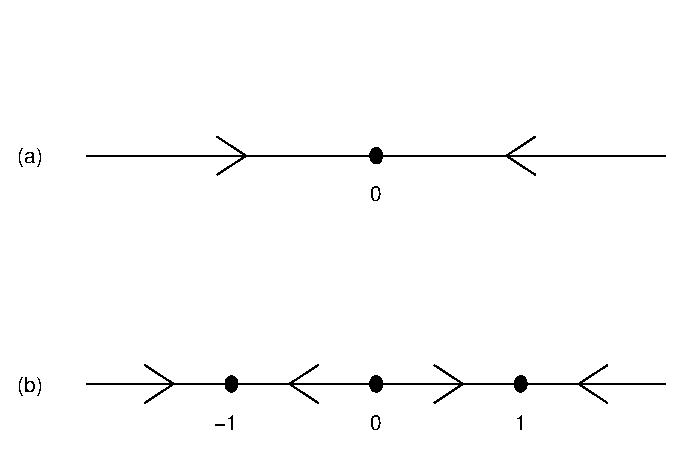
\psfig{file=figures/schemdyn.eps,width=3.4in}}
\caption{Schematic dynamics of (a) $\dot{x}=x(-1-x^2)$ and (b) $\dot{x}=x(1-x^2)$.}
\label{pitch3}
\end{figure}

\subsubsection*{Hyperbolic Equilibria}

Suppose that $x_0$ is an equilibrium for \Ref{aut}; that is suppose
$g(x_0)=0$.  We denote the derivative of $g(x)$ with respect to $x$, 
$dg/dx$, by $g'$.  The equilibrium $x_0$ is 
{\em hyperbolic\/} \index{hyperbolic}
if $g'(x_0)\neq 0$.  Assume that $x_0$ is a hyperbolic equilibrium and use
the tangent line approximation to $g(x)$ near $x_0$
($\Delta g = g'(x_0)\Delta x$) and that fact that $g(x_0)=0$ to conclude that
\[
g(x) \approx g'(x_0)(x-x_0).
\]
It follows that if $g'(x_0)<0$, then $g(x)$ is negative when
$x>x_0$ and positive when $x<x_0$.  So when $g'(x_0)<0$,
solutions of \Ref{aut} starting just to the right of $x_0$ will
move left ($g<0$) and tend towards $x_0$ and solutions starting
just to the left of $x_0$ will move right ($g>0$) and tend
towards $x_0$.  Similarly, if $g'(x_0)>0$, then $g(x)$ is positive
when $x>x_0$ and negative when $x<x_0$.  Thus, solutions near $x_0$ 
will tend away from $x_0$ when $g'(x_0)>0$.    We  have shown:
\begin{thm}[Stability of Hyperbolic Equilibria] \label{T:stability1}
Let $x_0$ be a hyperbolic equilibrium for the differential equation
\[
\frac{dx}{dt} = g(x).
\]
If $g'(x_0)<0$, then the equilibrium is asymptotically stable;
and if $g'(x_0)>0$, then the equilibrium is unstable.
\end{thm} \index{equilibrium} \index{stability!asymptotic}
\index{unstable}

It follows from Theorem~\ref{T:stability1} that the phase line picture
near a hyperbolic equilibrium is particularly simple as the arrows beside
that equilibrium either both point towards the equilibrium (as in
Figure~\ref{pitch3}(a)) or both point away from the equilibrium (as near $0$
in Figure~\ref{pitch3}(b)).

\subsection*{Comparing Phase Lines and Time Series}
\index{phase!line}\index{time series}

Phase line plots and time series graphs give different ways of
presenting the same information.  With that point in mind, it is
important to be able to recreate one type of plot from
the other.  For example, let $x(t)$ be the solution to the
differential equation $\dot{x}=x(1-x^2)$ with initial condition $x(0)=2$.
In Figure~\ref{pitch3}(b) we have drawn the schematic phase line for
all solutions to this differential equation. How can we reconstruct
a (schematic) graph of the time series $x(t)$ for this solution just
from the phase line?

To answer this question, note that in Figure~\ref{pitch3}(b) the
initial condition $x(0)=2$ lies to the right of all equilibria of
this equation, and the arrow indicates that solution trajectories
starting in this area move to the left, that is, they decrease to
the equilibrium at $x=1$.  It follows that
\[
\lim_{t\to\infty} x(t) = 1.
\]
Since there are no equilibria to the right of $x=2$, the graph of $x(t)$
must increase to infinity in {\em backwards\/} time.  So the graph of 
$x=x(t)$ is decreasing and asymptotic to $x=1$ for large positive $t$.  
A schematic graph is given in Figure~\ref{pitch3a}(a).  Using {\sf dfield5} 
we can check this description by numerically integrating the differential
equation.   This graph is shown in Figure~\ref{pitch3a}(b).

\begin{figure}[htb]
       \centerline{%
        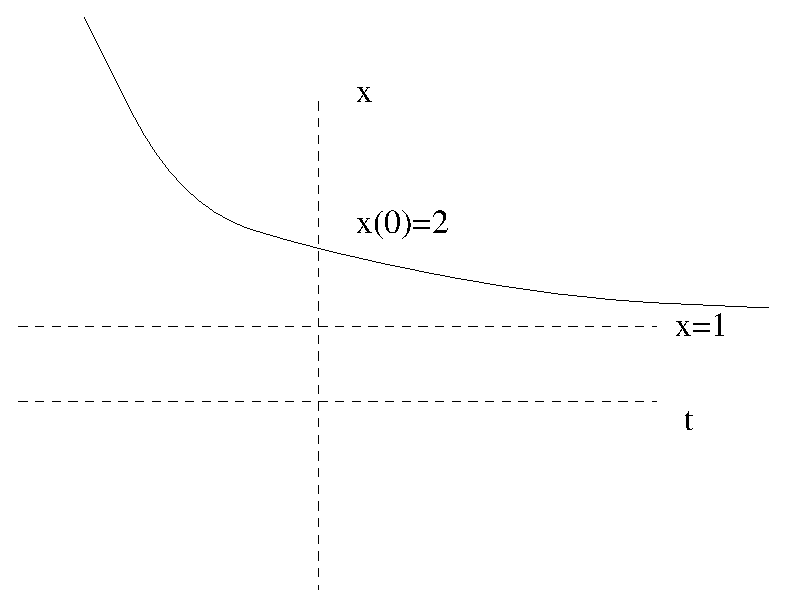
\psfig{file=figures/pitch3as.eps,width=2.8in}
	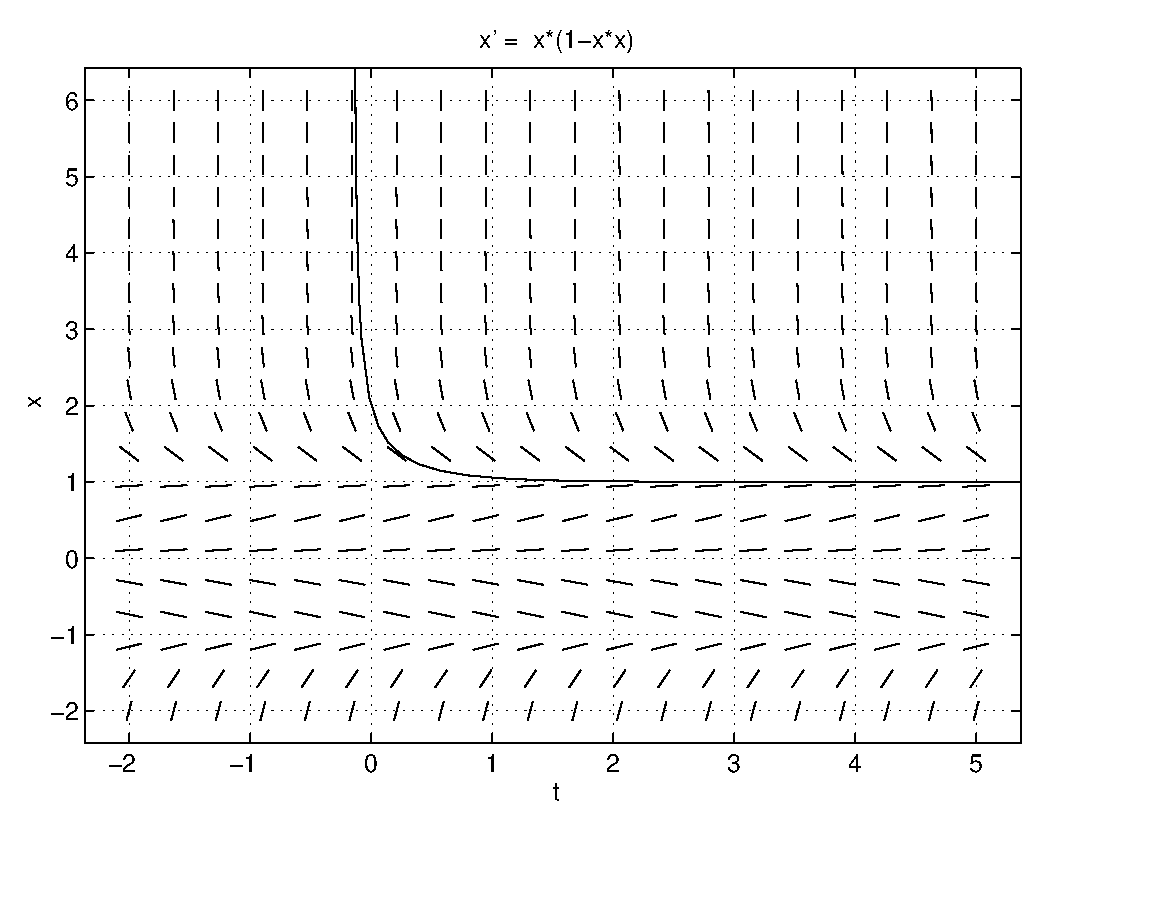
\psfig{file=figures/pitch3ad.eps,width=3.0in}}
       \caption{Time series for solution to $\dot{x}=x(1-x^2)$ with $x(0)=2$.
	(Left) Sketch using asymptotic information; (right) {\sf dfield5}
	computation.}
       \label{pitch3a}
\end{figure}



\EXER

\CEXER

\begin{exercise} \label{c3.3.1}
Use {\sf pline} to find an initial condition $x(0)$ for the
ordinary differential equation \Ref{lin1} with $\lambda=-0.2$
such that the corresponding solution $x(t)$ satisfies
$x(20)\in[0.001,0.002]$.
\end{exercise}

\begin{exercise} \label{c3.3.2}
Use {\sf pline} to find all the equilibria of the ordinary
differential equation
\[
\dot{x} = (x^2-1)(x+2).
\]
Which of the equilibria are stable and which are unstable?
\end{exercise}

\begin{exercise} \label{c3.3.3}
Consider the following ordinary differential equation:
\[
\dot{x} = \lambda x(1-x).
\]
Use {\sf pline} to find a value for the parameter $\lambda$ such
that $x(t)=1$ is a stable equilibrium.
\end{exercise}

\begin{exercise} \label{c3.3.4}
The differential equation
\[
\frac{dx}{dt} =  x^2
\]
has an equilibrium at the origin.  Use {\sf pline} to determine
those $x_0$ for which solutions to the initial value $x(0)=x_0$ tend
towards the origin.
\end{exercise}

\begin{exercise} \label{c3.3.5}
Consider the differential equation
\[
\frac{dx}{dt} = a x^3.
\]
Use {\sf pline} to verify that the origin is an asymptotically
stable equilibrium when $a = -1$ and is an unstable
equilibrium when $a = +1$. Discuss the relationship
between these examples and Theorem~\ref{T:stability1}.
\end{exercise}

\TEXER


\noindent In Exercises~\ref{c3.3.6A} -- \ref{c3.3.6D} compute the equilibria 
of the given differential equation, determine whether these equilibria are 
asymptotically stable or unstable, and draw a sche\-ma\-tic of the dynamics 
of this equation like the one in Figure~\ref{pitch3}.  You may use {\sf pline}
to check your answer.
\begin{exercise} \label{c3.3.6A}
$\dot{x} = x^2 + 2x - 3$.
\end{exercise}
\begin{exercise} \label{c3.3.6B}
$\dot{x} = x^3 - 2x^2 - 8x$.
\end{exercise}
\begin{exercise} \label{c3.3.6C}
$\dot{x} = x^3 + 2x^2 - 3x$.
\end{exercise}
\begin{exercise} \label{c3.3.6D}
$\dot{x} = x^2 + 6x + 1$.
\end{exercise}

\begin{exercise} \label{c3.3.7}
Let $x(t)$ be a solution to the initial value problem
\begin{eqnarray*}
\dot{x} & = & g(x) \\
x(0) & = & x_0.
\end{eqnarray*}
Let $y(t)=x(-t)$.  Show that $y(t)$ is a solution to the
initial value problem
\begin{eqnarray*}
\dot{y} & = & -g(y) \\
y(0) & = & x_0.
\end{eqnarray*}
(Thus, to integrate the solution $x(t)$ backwards in time is the
same as solving the differential equation $\dot{y}  =  -g(y)$
forward in time.)
\end{exercise}

\begin{exercise} \label{c3.3.9}
Use Exercise~\ref{c3.3.7} to devise a shortcut for solving
Exercise~\ref{c3.3.1}.
\end{exercise}

\begin{exercise} \label{c3.3.8}
Sketch the time series for the solution to the differential
equation pictured in Figure~\ref{pitch3}(b) with initial condition
$x(0)=\frac{1}{2}$.  Use only the phase space plot given in this
figure.  Use {\sf dfield5} to verify your answer.
\end{exercise}

\noindent In Exercises~\ref{c3.3.10a} -- \ref{c3.3.10d} use the line field 
given in Figure~\ref{F:exer3ad} to answer the following:\\
\noindent (a) Is the differential equation that was used to draw this figure 
autonomous or nonautonomous.\\
\noindent (b)  If the differential equation is autonomous, then draw the phase
line noting the values of $x$ where equilibria occur and whether they are 
asymptotically stable or not. If the differential equation is nonautonomous, 
then draw the time series for solutions with initial conditions $x(0)=0$ and 
$x(2)=0$.

\begin{exercise} \label{c3.3.10a}
Use Figure~\ref{F:exer3ad}(i) to answer parts (a) and (b).
\end{exercise}
\begin{exercise} \label{c3.3.10b}
Use Figure~\ref{F:exer3ad}(ii) to answer parts (a) and (b).
\end{exercise}
\begin{exercise} \label{c3.3.10c}
Use Figure~\ref{F:exer3ad}(iii) to answer parts (a) and (b).
\end{exercise}
\begin{exercise} \label{c3.3.10d}
Use Figure~\ref{F:exer3ad}(iv) to answer parts (a) and (b).
\end{exercise}

\begin{figure}[htb]
       \centerline{%
        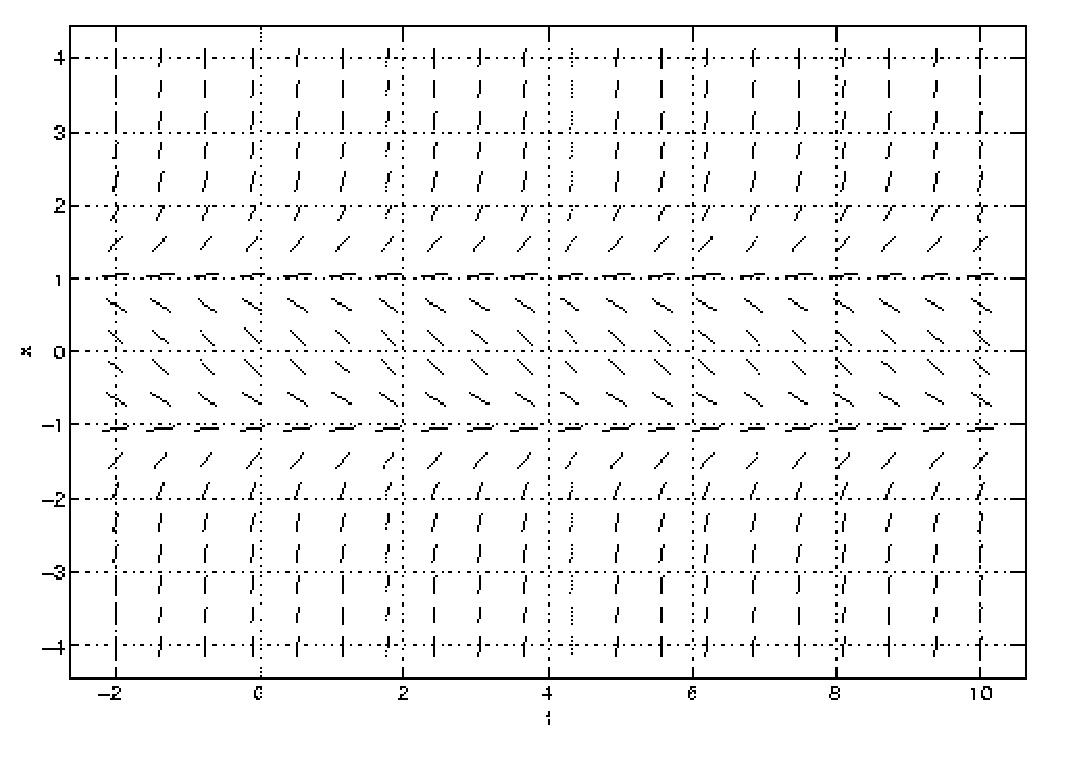
\psfig{file=figures/auto1a.eps,width=2.8in}
	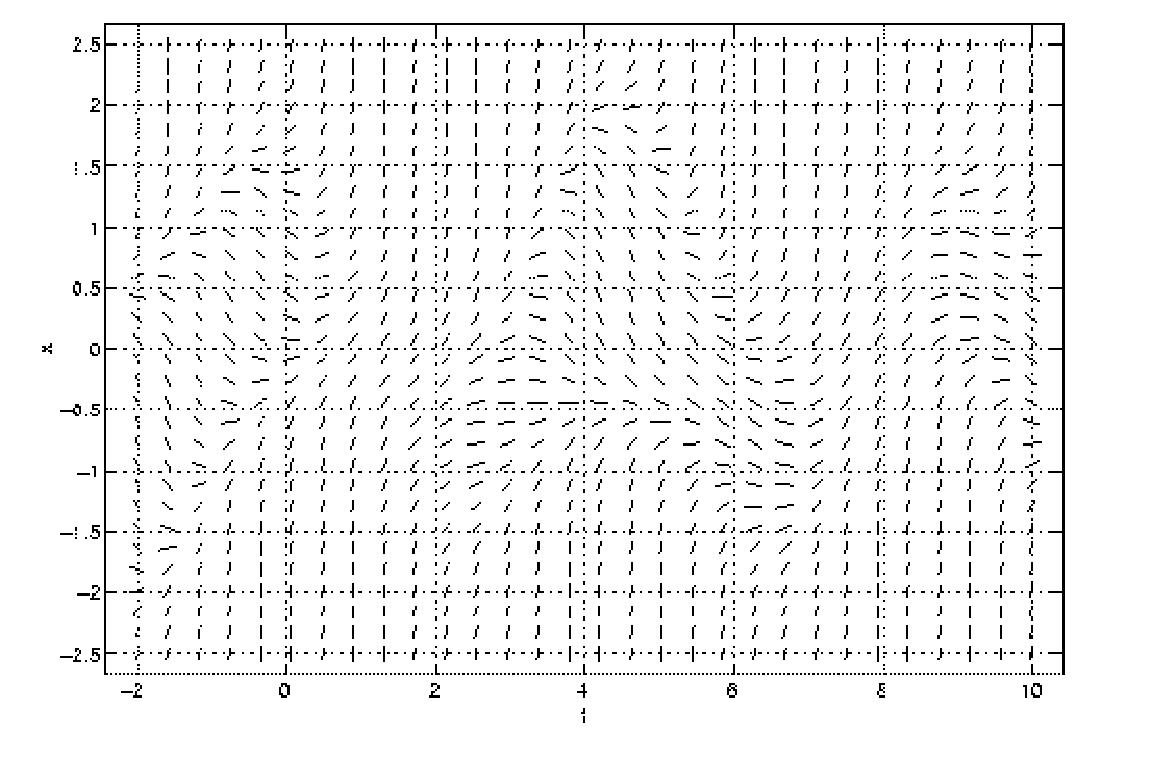
\psfig{file=figures/nonauto2a.eps,width=2.8in}}
\centerline{(i) \hspace{2.6in} (ii)}
       \centerline{%
        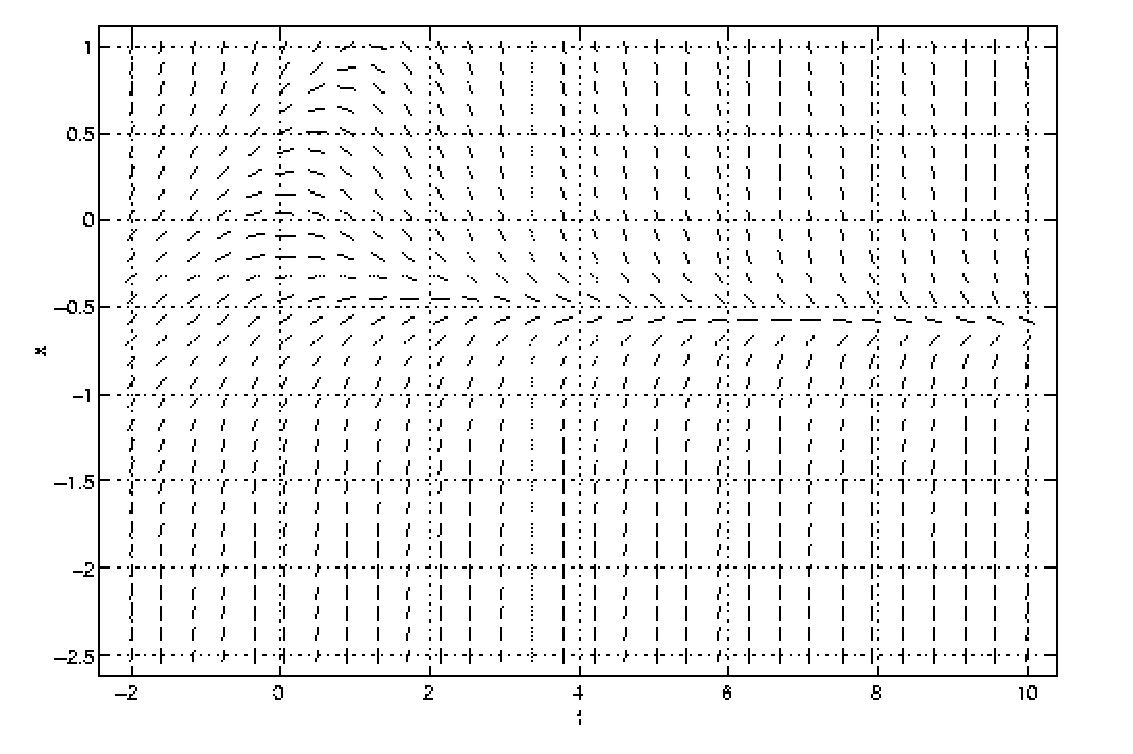
\psfig{file=figures/nonauto1a.eps,width=2.8in}
	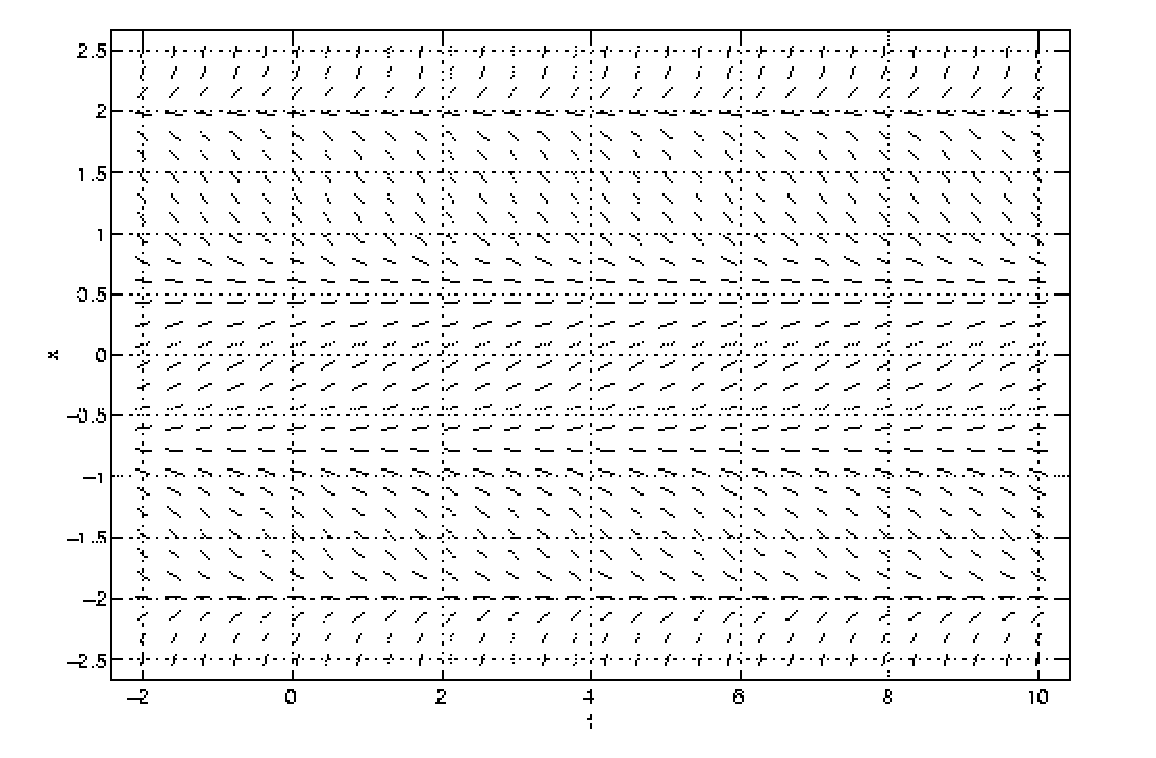
\psfig{file=figures/auto2a.eps,width=2.8in}}
\centerline{(iii) \hspace{2.6in} (iv)}
       \caption{Figures for Exercises~\protect{\ref{c3.3.10a}} --
\protect{\ref{c3.3.10d}}}
       \label{F:exer3ad}
\end{figure}


\Sec{*Separation of Variables}{SEPARATION OF VARIABLES}
\label{sec:sov} \index{separation of variables}

In this section we discuss a method for finding closed form solutions to
a particular class of nonautonomous first order ordinary differential 
equations\index{differential equation!first order} 
\begin{equation}  \label{e:nonauto}
\frac{dx}{dt} = f(t,x).
\end{equation}
These particular equations are {\em separable equations\/} having the form 
\begin{equation}  \label{eq:gh}
\frac{dx}{dt} = g(x) h(t),
\end{equation}
where $g,h:\R\to\R$ are continuous functions.   There are two special cases 
of \Ref{eq:gh}: the case $g(x)=1$ and the case $h(t)=1$.  

\subsubsection*{The Special Case $g(x)=1$: Integration Theory}

The assumption that $g(x)=1$ in \Ref{eq:gh} leads to the differential 
equation 
\begin{equation}  \label{e:g=1}
\frac{dx}{dt} = h(t).
\end{equation}
In Section~\ref{S:growthmodels} we saw that this differential equation  
is easily solved by direct integration.  For example, if $h(t)=t^2$ then 
the solution to \Ref{e:g=1} with initial condition $x(2)=5$ is found as
follows.  By direct integration,
\[
x(t) = \int t^2 dt = \frac{1}{3}t^3 + C.
\]
It then follows that
\[
x(2) = \frac{8}{3} + C = 5;
\]
so 
\[
C = 5 - \frac{8}{3} = \frac{7}{3}.
\]


\subsubsection*{The Special Case $h(t)=1$: Autonomous Equations}
\index{autonomous}

The second special case in \Ref{eq:gh} leads to the autonomous 
differential equation
\begin{equation}  \label{e:h=1}
\frac{dx}{dt} = g(x).
\end{equation}
Begin by noting that equilibria are special solutions to \Ref{e:h=1} that we 
can find by solving the equation $g(x)=0$.  More precisely, if $g(x_0)=0$, 
then $x(t)=x_0$ is a constant solution to \Ref{e:h=1}.  

We find the 
nonequilibrium solutions by direct integration --- but only after 
using change of variables in integration.  To solve \Ref{e:h=1},
just divide both sides of this equation by $g(x)$, obtaining
\[
\frac{1}{g(x)}\frac{dx}{dt} = 1,
\]
and integrate with respect to $t$, obtaining
\[
\int \frac{1}{g(x)} \frac{dx}{dt} dt = \int dt + C = t + C.
\]
After substituting $y=x(t)$ and using the chain rule, the integral on 
the left becomes
\[
\int\frac{1}{g(y)}dy.
\]
Replacing $y$ by $x$, we obtain
\[
\int\frac{1}{g(x)}dx = t + C.
\]

As a simple example, solve the growth rate equation \Ref{lin1} 
\begin{equation}  \label{lin1a} 
\frac{dx}{dt} = \lambda x
\end{equation}
using this technique of integration.  It follows that 
\[
\int \frac{1}{x}dx = \lambda t + C.
\]
So, to solve \Ref{lin1a}, we need to know how to integrate the function 
$1/x$.  Recalling that this integral is just $\ln |x|$ we obtain
\[
\ln |x(t)| = \lambda t + C.
\]
We solve this equation by exponentiation, obtaining
\[
|x(t)| = K e^{\lambda t},
\]
where $K = e^C \geq 0$.  On dropping the absolute value signs, we obtain
\[
x(t) =   K e^{\lambda t},
\]
for arbitrary $K$.  Of course, this is precisely the solution that we 
found in \Ref{soln1}.  

It is worth reflecting on the information from calculus that we needed to 
solve \Ref{lin1a}.  In Section~\ref{S:growthmodels} we found the solution to 
this equation by asking what function has a derivative that is a multiple of 
itself.  We then had to remember that $e^{\lambda t}$ is such a function and 
then prove that up to the constant $K$ this was the only such function 
(recall Theorem~\ref{T:singleeqn}).  Here we needed to remember the 
indefinite integral of $1/x$ and then solve for $x$ in terms of $t$.  

We now summarize this technique for solving the autonomous differential 
equation \Ref{e:h=1}.  Let $G(x)$ be an indefinite integral of $1/g(x)$. 
Then, after division by $g(x)$, integrating both sides of \Ref{e:h=1} 
with respect to $t$ leads to the equation 
\[
G(x) = t + C.
\]
Then we need to solve this algebraic equation for $x$ in terms of $t$.  This
last step is often quite difficult, as we show by example below.

There is one additional point that needs to be remembered when using 
this technique.  The constant $C$ is, as usual, related to an initial
condition.  Indeed, if we wish to solve \Ref{e:h=1} with the initial
condition $x(t_0)=x_0$, then we can solve for 
\[
C = G(x_0) - t_0.
\]

\subsubsection*{An Example of Blow-up in Finite Time}
\index{blow-up in finite time}

Consider the nonlinear differential equation
\begin{equation}  \label{e:x^2}
\frac{dx}{dt} = x^2
\end{equation}
satisfying the initial condition $x(t_0)=x_0$.  Using the preceding 
discussion, we can solve \Ref{e:x^2} by integration.  Specifically,
on division we obtain
\[
\frac{1}{x^2}\frac{dx}{dt} = 1,
\]
and on integration with respect to $t$, we obtain
\[
-\frac{1}{x} = t + C.
\]
Solving for $x$ in terms of $t$ we obtain
\[
x(t) = - \frac{1}{t+C}.
\]
Finally, use the initial condition to solve for $C$. On substitution 
\[
x_0 = x(t_0) = - \frac{1}{t_0+C}.
\]
Hence
\[
C = -\frac{1}{x_0} - t_0,
\]
which is fine unless $x_0$ happens to equal $0$.  However, in that case, we 
have just recovered the equilibrium solution $x(t)=0$.

On setting
\[
K = \frac{1}{x_0}+t_0,
\]
we obtain the solution
\[
x(t) =  \frac{1}{K-t}.
\]
For example, if $t_0=0.1$ and $x_0=2$, then $K=0.6$ and
\begin{equation} \label{E:solnx^2}
x(t) = \frac{1}{0.6-t}.
\end{equation}

Example~\Ref{e:x^2} shows that solutions to nonlinear differential
equations\index{differential equation!nonlinear} possess 
qualitative properties that are different from 
those of the linear equation $\dot{x}=\lambda x$.  In particular:
\begin{itemize}
\item Solutions can approach infinity in finite time.   For example, 
the solution \Ref{E:solnx^2} with initial condition $x(0.1)=2$ goes to 
infinity as $t$ approaches $0.6$.   
\item Solutions may not be defined for all $t\in\R$.  Indeed, the 
solution \Ref{E:solnx^2} has a singularity at $t=0.6$ and is defined 
for either $t> 0.6$ or $t<0.6$.  
\end{itemize}


We can solve equation \Ref{e:x^2} using 
{\sf dfield5}\index{\computer!dfield5}.
Using {\sf Keyboard input} set the initial condition at
$(x_0,t_0)=(2,0.1)$ and obtain the trajectory in
Figure~\ref{F:x^2}(left).  Note that this solution goes to infinity
in forward time while approaching $t=0.6$.  Now set the initial
condition to $(x_0,t_0)=(1,-2.5)$ and see that the solution goes
to negative infinity as $t$ approaches $0.6$ from above.  See
Figure~\ref{F:x^2}(right).  Finally note that both of these
solutions are given by the same formula \Ref{E:solnx^2}.

\begin{figure}[htb]
           \centerline{%
           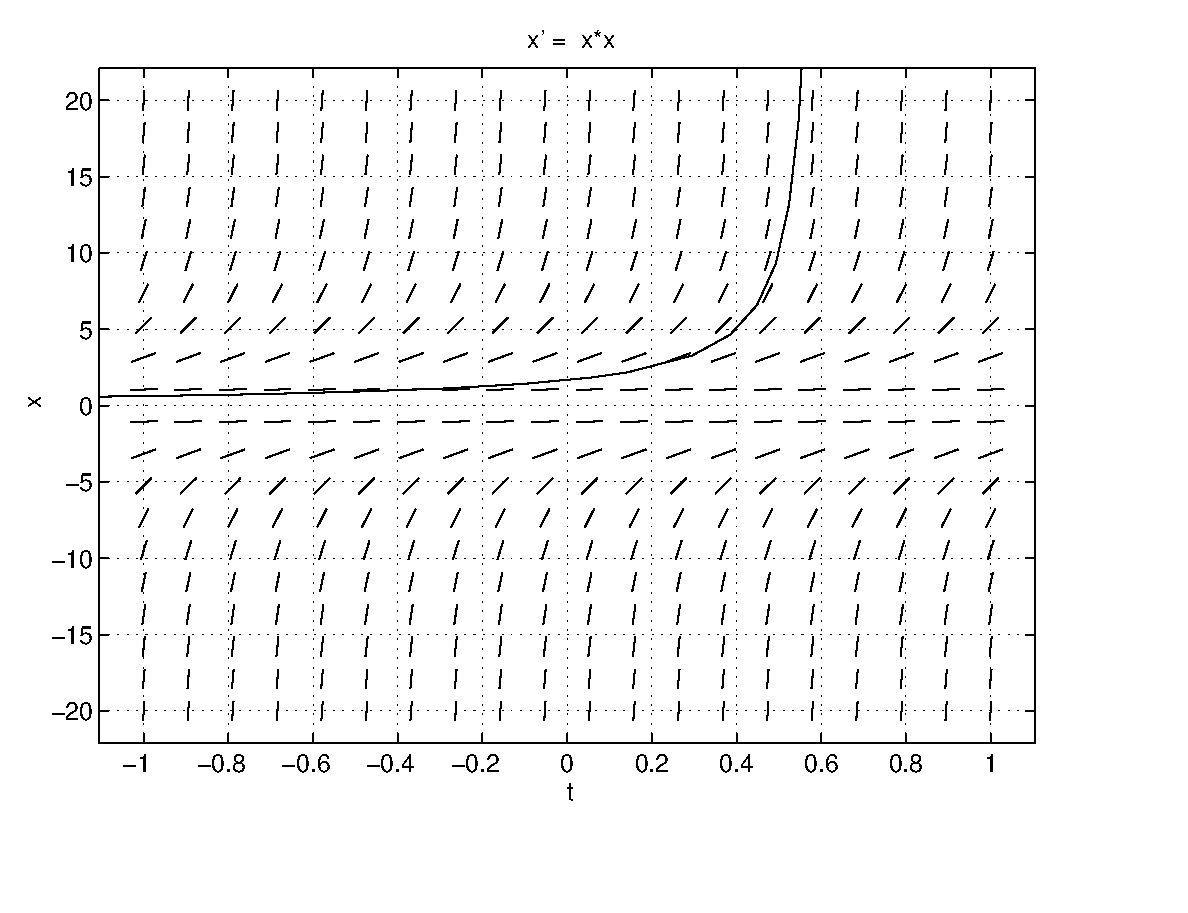
\psfig{file=figures/x2a.eps,width=3.5in}
	   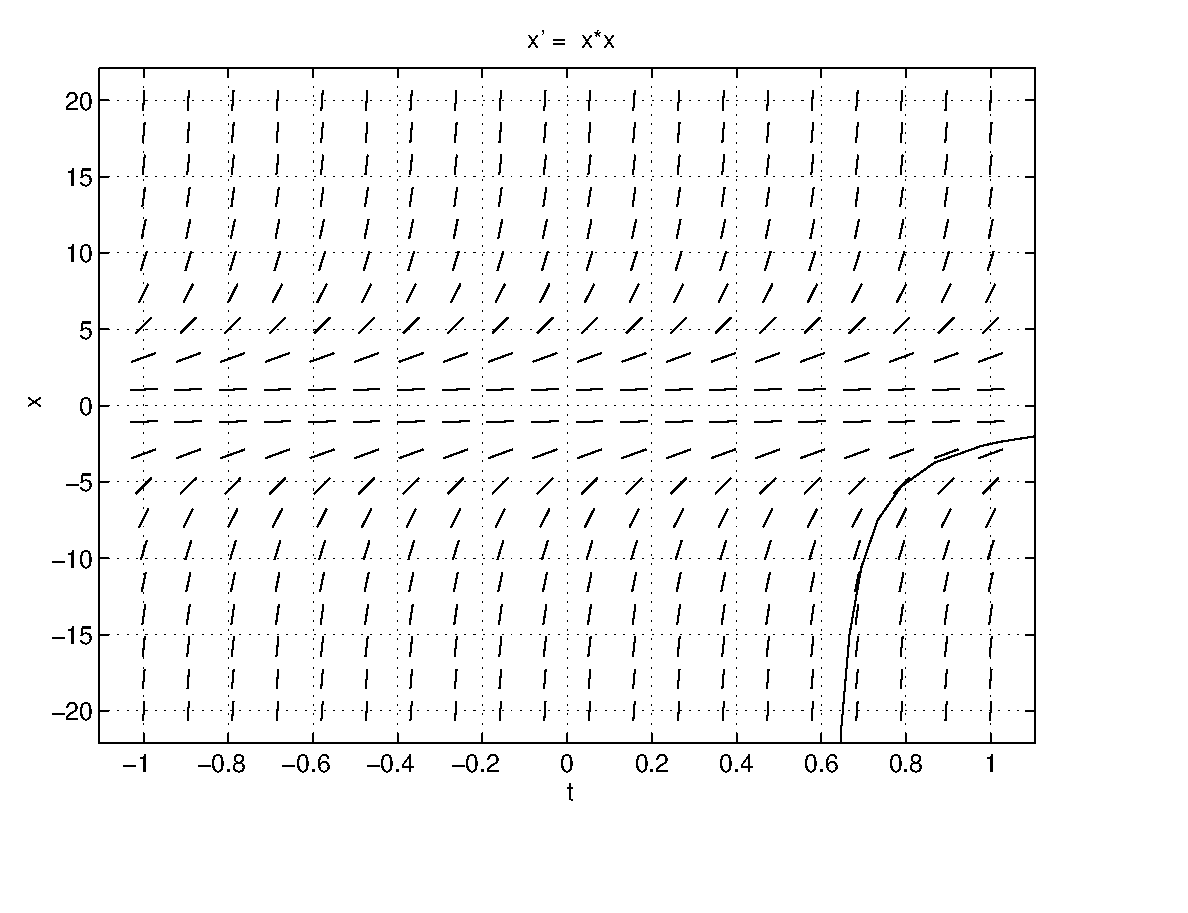
\psfig{file=figures/x2b.eps,width=3.5in}}
           \caption{Solutions using {\sf dfield5} for $\frac{dx}{dt} = x^2$ 
		with initial conditions: (left) $(x_0,t_0)=(2,0.1)$ and 
		(right) $(x_0,t_0)=(1,-2.5)$.}
           \label{F:x^2}
\end{figure}

\subsubsection*{An Example that Cannot be Solved in Closed Form}

Consider the differential equation
\begin{equation}  \label{E:ncf}
\frac{dx}{dt} = \frac{x}{x-1}
\end{equation}
with initial condition $x(1)=2$. On division \Ref{E:ncf} becomes 
\[
\left(1-\frac{1}{x}\right)\frac{dx}{dt} = 1.
\]
Integration with respect to $t$ yields
\[
x - \ln|x| = t + C.
\]
Using the initial condition, we see that 
\[
C = 2 - \ln 2 -1 = 1 - \ln 2.
\]
Note that for $t$ near $1$, the initial condition implies that $x(t)>0$.  
Hence $x(t)$ satisfies
\begin{equation} \label{e:solnncf}
x -\ln x = t + 1 - \ln 2.
\end{equation}
Unfortunately, this equation cannot be solved explicitly for $x$ 
as a function of $t$; that is, there is no closed form 
solution\index{closed form solution} 
for $x(t)$.  Nevertheless, $x(t)$ is defined 
{\em implicitly\/}\index{solution!implicitly defined} 
by \Ref{e:solnncf}.  This equation can, however, be solved numerically by
{\sf dfield5} just as easily as equations that have closed form solutions.
See Exercise~\ref{c14.1.17}. 

\subsection*{The General Solution by Separation of Variables}
\index{separation of variables!general solution}

The solution to the initial value problem for the separation
of variables equation
\begin{equation}  \label{eq:ghivp}
\dps \frac{dx}{dt} =  g(x) h(t),
\end{equation}
where $x(t_0) = x_0$, is obtained by combining the integrations of the two 
special cases just considered.  

Note that if $g(x_0)=0$, then $x(t)=x_0$ is an equilibrium solution to 
\Ref{eq:ghivp}.  So we can assume 
\begin{equation} \label{eq:gx0}
g(x_0)\not=0,
\end{equation}
and divide \Ref{eq:ghivp} by $g(x)$ to obtain
\[
\frac{1}{g(x)}\frac{dx}{dt}= h(t).
\]
Integrating with respect to $t$ yields
\[
\int \frac{1}{g(x)} \frac{dx}{dt}dt = \int h(t) dt + C.
\]
As before, on changing variables, we obtain
\[
\int\frac{1}{g(x)} dx = \int h(t) dt.
\]
Thus, the abstract solution to \Ref{eq:ghivp} can be written as
\begin{equation} \label{E:G=H+K}
G(x) = H(t) + C,
\end{equation}
where $G$ is an indefinite integral of $1/g$ and $H$ is an indefinite 
integral of $h$, and 
\begin{equation}  \label{E:G=H+Kinit}
C = G(x_0)-H(t_0).
\end{equation}



\subsubsection*{An Example Solving the Initial Value Problem}
\index{separation of variables!initial value problem}

We illustrate the technique of separation of variables with the following
example.  Find the solution of the initial value problem
\[
\frac{dx}{dt} = \frac{t}{x^2} 
\]
where $x(1)=2$.  Here $g(x) = 1/x^2$ and $h(t) = t$, so that
\[
G(x)=\int x^2 dx= \frac{1}{3}x^3 \AND H(t) = \int t dt = \frac{1}{2}t^2.
\]
Since $t_0=1$ and $x_0=2$, we can use \Ref{E:G=H+Kinit} to see that 
\[
C = G(2)-H(1) = \frac{8}{3} -\frac{1}{2} = \frac{13}{6},
\]
and \Ref{E:G=H+K} to see that the solution $x(t)$ satisfies
\[
\frac{1}{3}x(t)^3 = \frac{1}{2}t^2 + \frac{13}{6}.
\]
Therefore,
\[
x(t) = \left(\frac{3t^2+13}{2}\right)^{1/3}.
\]
The reader may check that this function is indeed a solution
satisfying the specified initial condition.

\subsubsection*{An Example Finding a General Solution}
\index{separation of variables!general solution}

With this example, we illustrate how to use separation of variables to find 
all solutions of a differential equation in the form \Ref{eq:gh}.  Consider
\begin{equation} \label{eq:x1t2}
\frac{dx}{dt} = \frac{(x+1)(t^2+1)}{t}
\end{equation}
for $t>0$.  Using our notation we have 
\[
g(x) = x+1 \AND h(t) = t+\frac{1}{t}.
\]
Note that $g(-1)=0$ and hence that $x(t)=-1$ is the constant equilibrium 
solution to \Ref{eq:x1t2}.  For all the other initial conditions, we obtain 
\[
G(x)=\int \frac{1}{x+1} dx = \ln|x+1| \AND 
H(t) = \int\left(t + \frac{1}{t}\right)dt = \frac{1}{2}t^2 + \ln |t|.
\]
Thus, in this example, identity \Ref{E:G=H+K} implies that the 
solution $x(t)$ satisfies
\[
\ln |x(t)+1| = \frac{1}{2}t^2 + \ln |t| + C.
\]
Hence
\[
|x(t)+1| = K|t|e^{t^2/2},
\]
for some constant $K>0$ and nonconstant solutions of \Ref{eq:x1t2} are in 
one-to-one correspondence with functions
\[
x(t) = Kte^{t^2/2}-1
\]
for $K\in\R$.  Note that setting $K=0$ recovers the constant solution 
$x(t)=-1$.

\EXER

\TEXER

\noindent In Exercises~\ref{c14.1.1a} -- \ref{c14.1.1d} decide whether 
or not the method of separation of variables can be applied to the given
differential equation.  If this method can be applied, then specify the 
functions $g$ and $h$ --- but do not perform the integrations.
\begin{exercise} \label{c14.1.1a}
$\dps \frac{dx}{dt} = x^{1/2}\cos t$.
\end{exercise}
\begin{exercise} \label{c14.1.1b}
$\dps \frac{dx}{dt} = (x+xt)\tan x$.
\end{exercise}
\begin{exercise} \label{c14.1.1c}
$\dps \frac{dx}{dt} = (x+t)(x-t)$.
\end{exercise}
\begin{exercise} \label{c14.1.1d}
$\dps \frac{dx}{dt} = 3-2x+3t-2xt$.
\end{exercise}

\noindent In Exercises~\ref{c14.1.5a} -- \ref{c14.1.5c} solve the given 
initial value problem by separation of variables. 
\begin{exercise}  \label{c14.1.5a}
$\dps \frac{dx}{dt} = -3x,\quad x(0)=-1.$
\end{exercise}
\begin{exercise}  \label{c14.1.5b}
$\dps \frac{dx}{dt} = \frac{t^3-1}{\cos x},
\quad x(\pi)=\frac{\pi}{2}.$
\end{exercise}
\begin{exercise}  \label{c14.1.5c}
$\dps \frac{dx}{dt} = 2\sqrt{tx},\quad x(1)=1.$
\end{exercise}

\noindent In Exercises~\ref{c14.1.8a} -- \ref{c14.1.8c} use separation 
of variables to find all the solutions of the given differential equation.
\begin{exercise}  \label{c14.1.8a}
$\dps \frac{dx}{dt} = 2x$.
\end{exercise}
\begin{exercise}  \label{c14.1.8b}
$\dps \frac{dx}{dt} = 5x+2$.
\end{exercise}
\begin{exercise}  \label{c14.1.8c}
$\dps \frac{dx}{dt} = \frac{\sin t}{x}$.
\end{exercise}

\CEXER

\noindent We have studied the autonomous linear differential equation 
$\dot{x}=\lambda x$ when $\lambda\neq 0$ and have shown that solutions 
exist for all time and tend either to $0$ or to $\pm\infty$ as $t\to\pm\infty$.
See \Ref{explimits} and Figure~\ref{df_dsp1}.  In Exercises~\ref{c14.1.11a} -- 
\ref{c14.1.11f} explore the behavior of solutions $x(t)$ of the given 
nonlinear (and often nonautonomous) differential equation using {\sf dfield5}.  
Where possible, describe the differences between the behavior of solutions of 
the given differential equation and the linear differential equation.  

\noindent{\bf Hint:}  Here is a list of properties of solutions that are 
{\em not valid\/} for solutions to the linear differential equation:
\begin{itemize}
\item[(a)]  Solutions blow up in finite time (that is, 
$\lim_{t\to t_0}x(t)=\pm\infty$).
\item[(b)]  Solutions do not exist for all time.
\item[(c)]  Multiple solutions are bounded in both forward and backward time.
(In the linear system only the zero solution $x(t)=0$ is bounded in both 
forward and backward time.)
\item[(d)]  Solutions stop (that is, solutions limit in either forward or 
backward time on a finite value of $x$ in finite time $t$).
\end{itemize}
Use {\sf dfield5} to determine which of these properties of solutions are 
valid for the given differential equations.  Also, when exploring 
Exercises~\ref{c14.1.11a} -- \ref{c14.1.11f} be prepared to use the {\sf Stop}
button in the {\sf DFIELD5 Display} window to stop the numerical integration. 

\begin{exercise} \label{c14.1.11a}
$\dps\frac{dx}{dt} = \frac{1}{x}$.
\end{exercise}
\begin{exercise} \label{c14.1.11b}
$\dps\frac{dx}{dt} = \frac{1}{tx}$.
\end{exercise}
\begin{exercise} \label{c14.1.11c}
$\dps\frac{dx}{dt} = \sin(tx)$.
\end{exercise}
\begin{exercise} \label{c14.1.11d}
$\dps\frac{dx}{dt} = t^2 - x^3$.
\end{exercise}
\begin{exercise} \label{c14.1.11e}
$\dps\frac{dx}{dt} = x(1-x^2)$.
\end{exercise}
\begin{exercise} \label{c14.1.11f}
$\dps\frac{dx}{dt} = \frac{t}{x^2}$.
\end{exercise}

\begin{exercise} \label{c14.1.17}
Recall that the differential equation \Ref{E:ncf} $\dot{x}=x/(x-1)$ cannot be 
solved in closed form.  
\begin{itemize}
\item[(a)]	Use {\sf dfield5}\index{\computer!dfield5} 
to solve this differential 
equation numerically on the interval $0.8\leq t\leq 1.2$ with initial 
condition $x(1)=2$.  (Set the $x$ interval to be $[0,4]$.)  
\item[(b)]	Using this result estimate the value of $x(1.15)$ to two 
decimal places.
\item[(c)]	Next change the time interval to be $0.5\leq t\leq 1.2$.
The numerically computed solution $x(t)$ behaves strangely when $t\leq 0.7$. 
What is the approximate value of $x$ in this range of $t$?  Use this 
observed value to explain why the numerical integration for this differential 
equation is badly behaved.
\end{itemize}
\end{exercise}

\begin{exercise} \label{c14.1.18}
The ability to find closed form solutions to differential equations enables
us to test the accuracy of numerically computed solutions.  As an example where difficulties arise in numerical computations, consider the differential 
equation
\begin{equation} \label{eq:exivp}
\frac{dx}{dt} = \left(\frac{x}{t}\right)^2.
\end{equation}
\begin{itemize}
\item[(a)] Use separation of variables to find the solution $x(t)$ to the 
initial value problem $x(0.001) = 2/1999$ of \Ref{eq:exivp}.
\item[(b)] Show that $\dps\lim_{t\to 2^-}x(t)=\infty$ for the solution of 
\Ref{eq:exivp} obtained in (a).
\item[(c)] For the initial condition specified in (a) compare the analytic 
solution of \Ref{eq:exivp} to the numerical solution computed by {\sf dfield5} 
in the region where the maximum value of $t$ is $2.5$ and the maximum value of 
$x$ is $100$.  How does the behavior of the numerically computed solution 
to \Ref{eq:exivp} differ from that of the analytically computed solution?
\item[(d)]  Compute the solution of \Ref{eq:exivp} using the general initial 
condition $x(t_0) = x_0$ where $t_0,x_0>0$ and show that 
$\lim_{t\to 0^+}x(t)=0$ for every such solution. 
\end{itemize}
\noindent {\bf Comment:} Part (d) hints at why there is a discrepancy 
between the numerically approximated solution and the analytic solution: 
small errors in the approximate solution with initial condition $(t_0,x_0)$ 
near $(0,0)$ cause different solutions to be computed.
\end{exercise}

 

\section{Uncoupled Linear Systems of Two Equations}
\label{sec:UncoupledLS}

An autonomous system of two (first order) \index{first order}
differential equations \index{system of differential equations}
has the form
\renewcommand{\arraystretch}{1.8}
\begin{equation} \label{e:aut2}
\begin{array}{lll}
\dps \frac{dx}{dt}(t)  & = & f(x(t),y(t)) \\
\dps \frac{dy}{dt}(t)  & = & g(x(t),y(t)),
\end{array}
\end{equation}
where $f$ and $g$ are functions of the two variables $x$
and $y$.  Solutions to \Ref{e:aut2} are pairs of functions
$(x(t),y(t))$.

As in the single equation \Ref{aut}, the simplest
solutions are equilibria.  An {\em equilibrium\/} \index{equilibrium}
solution to
\Ref{e:aut2} is a solution where both functions $x(t)$
and $y(t)$ are constant functions; that is,
\[
x(t) = x_0 \AND  y(t)=y_0.
\]
For equilibria, it follows that both
\[
\frac{dx}{dt} = 0 \AND \frac{dy}{dt} = 0.
\]
Hence, equilibria of \Ref{e:aut2} can be found by
simultaneously solving the equations
\begin{eqnarray*}
f(x,y) & = & 0 \\
g(x,y) & = & 0.
\end{eqnarray*}

An autonomous {\em linear\/} system \index{linear!system} of ordinary
differential equations \index{system of differential equations!linear}
has the form
\renewcommand{\arraystretch}{1.8}
\begin{equation} \label{e:autlin}
\begin{array}{lll}
\dps \frac{dx}{dt}(t)  & = & a x(t) + b y(t) \\
\dps \frac{dy}{dt}(t)  & = & c x(t) + d y(t),
\end{array}
\end{equation}
\renewcommand{\arraystretch}{1.0}%
where $a,b,c,d$ are real constants.  Note that the origin
$(x(t),y(t))=(0,0)$ is always an equilibrium for a linear
system.

We begin our discussion of linear systems of ordinary
differential equations by considering uncoupled
\index{system of differential equations!uncoupled}systems of the form
\renewcommand{\arraystretch}{1.8}
\begin{equation} \label{lin2}
\begin{array}{lll}
\dps \frac{dx}{dt}(t) & = & a x(t) \\
\dps \frac{dy}{dt}(t) & = & d y(t).
\end{array}
\end{equation}
\renewcommand{\arraystretch}{1.0}%
Since the system is {\em uncoupled\/} (that is, the equation for
$\dot{x}$ does not depend on $y$ and the equation for $\dot{y}$
does not depend on $x$), we can solve this system by solving each
equation independently, as we did for \Ref{lin1}:
\begin{equation} \label{e:explicitsoln}
\begin{array}{ccc}
x(t) & = & x_0e^{at} \\
y(t) & = & y_0e^{dt}.
\end{array}
\end{equation}
There are now two initial conditions that are identified by
\[
x(0) = x_0 \AND y(0) = y_0.
\]

Having found all the solutions to \Ref{lin2} in \Ref{e:explicitsoln},
we now explore the geometry of the phase plane for
these uncoupled systems both analytically and by using \Matlabp.


\subsection*{Asymptotic Stability of the Origin}

As we did for the single equation \Ref{lin1}, we ask
what happens to solutions to \Ref{lin2} starting at $(x_0,y_0)$ as
time $t$ increases.  That is, we compute
\[
\lim_{t\to\infty}(x(t),y(t))=\lim_{t\to\infty}(x_0e^{a t},y_0e^{d t}).
\]
This limit is $(0,0)$ when both $a<0$ and $d<0$; but
if either $a$ or $d$ is positive, then most solutions diverge
to infinity, since either
\[
\lim_{t\to\infty}|x(t)| =\infty \quad \mbox{ or } \quad
\lim_{t\to\infty}|y(t)| =\infty.
\]


Roughly speaking, an equilibrium \index{equilibrium} $(x_0,y_0)$ is 
{\em asymptotically stable\/} \index{stability!asymptotic} if every 
trajectory $(x(t),y(t))$ beginning from an initial condition near 
$(x_0,y_0)$ stays near $(x_0,y_0)$ for all positive $t$, and
\[
\lim_{t\to\infty}(x(t),y(t)) = (x_0,y_0).
\]
The equilibrium is {\em unstable\/} \index{unstable} if there are  
trajectories with initial conditions arbitrarily close to the 
equilibrium that move far away from that equilibrium.

At this stage, it is not clear how to determine whether the
origin is asymptotically stable for a general linear system
\Ref{e:autlin}.  However, for uncoupled linear systems we
have shown that the origin is an asymptotically stable
equilibrium when both $a < 0$ and $d < 0$.  If either
$a >0$ or $d > 0$, then $(0,0)$ is unstable.

\subsubsection*{Invariance of the Axes}

There is another observation that we can make
for uncoupled systems.  Suppose that the initial condition for
an uncoupled system lies on the $x$-axis; that is, suppose $y_0=0$.
Then the solution $(x(t),y(t))=(x_0e^{at},0)$ also lies on the
$x$-axis for all time.  Similarly, if the initial condition lies
on the $y$-axis, then the solution $(0,y_0e^{dt})$ lies on the
$y$-axis for all time.

This invariance of the coordinate axes for uncoupled systems
follows directly from \Ref{e:explicitsoln}.  It turns out that
many linear systems of differential equations have invariant
lines; this is a topic to which we return later in this chapter.

\subsection*{Generating Phase Space Pictures with {\sf pplane5}}
\index{\computer!pplane5}

How can we visualize a solution $(x(t),y(t))$ to a system of
differential equations \Ref{e:aut2}?  The time series approach
suggests that we should graph $(x(t),y(t))$ as a function of $t$;
that is, we should plot the curve
\[
(t,x(t),y(t))
\]
in three dimensions.  Using \Matlab it is
possible to plot such a graph --- but such a graph by itself is
difficult to interpret.  Alternatively, we could graph either of
the functions $x(t)$ or $y(t)$ by themselves as we do for
solutions to single equations --- but then some information is
lost.

The method we prefer is the {\em phase space\/}\index{phase!space} 
plot obtained by thinking of $(x(t),y(t))$ as the
position of a particle in the $xy$-plane at time $t$.  We then
graph the point $(x(t),y(t))$ in the plane as $t$ varies.  When
looking at phase space plots, it is natural to call solutions
{\em trajectories\/},\index{trajectory} since we can imagine
that we are watching a particle moving in the plane as time
changes.

We begin by considering uncoupled linear equations.  As we saw,
when the initial conditions are on the coordinate axes (either
$(x_0,0)$ or $(0,y_0)$), the solutions remain on the coordinate
axes.  For these initial conditions, the equations behave as if
they were one dimensional.  However, if we consider an initial
condition $(x_0,y_0)$ that is not on a coordinate axis, then even
for an uncoupled system it is a little difficult to
{\em see\/} what the trajectory looks like.  At this point
it is useful to use the computer.

The method used to integrate planar systems of autonomous
differential equations is similar to that used to integrate
nonautonomous single equations in {\sf dfield5}.  The solution
curve $(x(t),y(t))$ to \Ref{e:aut2} at a point $(x_0,y_0)$ is
tangent to the direction $(f(x_0,y_0),g(x_0,y_0))$.  So
the differential equation solver plots the direction field
\index{direction field}
$(f,g)$ and then finds curves that are tangent to these
vectors at each point in time.

The program {\sf pplane5}\index{\computer!pplane5}, written by John
Polking,\index{Polking, John} is the two-dimensional analog of {\sf pline}.  
In \Matlab type
\begin{verbatim}
pplane5
\end{verbatim}
and the window with the {\sf PPLANE5 Setup} appears. {\sf pplane5}
has a number of preprogrammed differential equations listed in a
menu accessed by clicking on {\sf Gallery}.  To explore linear
systems, choose {\sf linear system} in the {\sf Gallery}.  (Note that the 
parameters in the {\sf linear system} are given by capitals rather than 
lower case {\sf a,b,c,d}.)

To integrate the uncoupled linear system, set the parameters $b$
and $c$ equal to zero. We now have the system \Ref{lin2} with
$a = 2$ and $d = -3$.  After pushing {\sf Proceed}, a display window
similar to {\sf dfield5} appears.  The main difference is that
the plane is filled by vectors $(f,g)$ indicating directions,
rather than by line segments indicating slopes.

As with {\sf dfield5} we may start the computations by clicking
with a mouse button on an initial value $(x_0,y_0)$.  For example,
if we click approximately onto $(x(0),y(0))=(x_0,y_0)=(1,1)$, then
the trajectory in the upper right quadrant of
Figure~\ref{pp_dsp1} displays.

\begin{figure}[htb]
     \centerline{%
     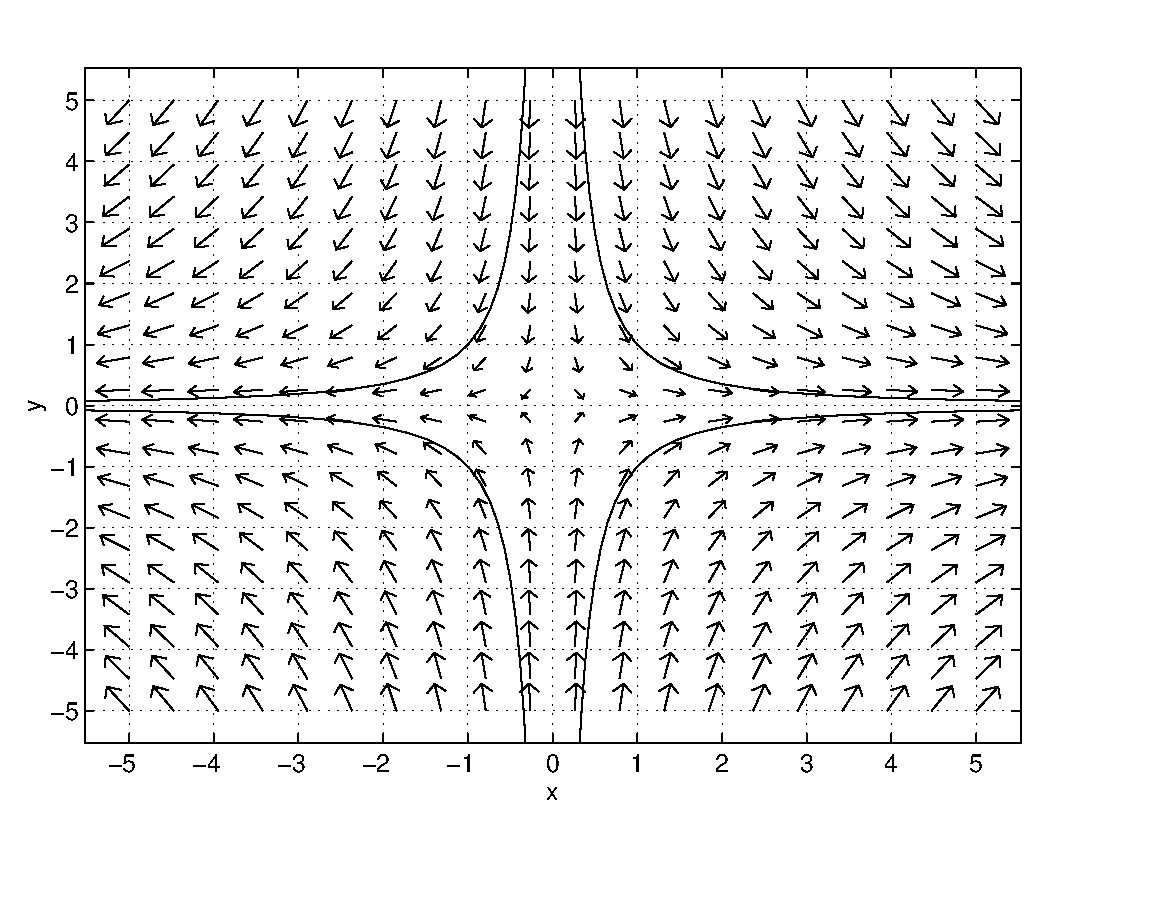
\psfig{file=figures/pp_dsp1.eps,width=3.5in}}
     \caption{{\sf PPLANE5 Display} for \protect\Ref{lin2} with
             $a=2$, $d=-3$ and $x,y\in [-5,5]$. Solutions
             going through $(\pm 1,\pm 1)$ are shown.}
     \label{pp_dsp1}
\end{figure}

First {\sf pplane5} draws the trajectory in forward time for
$t\ge 0$ and then it draws the trajectory in backwards time for
$t\le 0$.  More precisely, when we click on a point $(x_0,y_0)$ in
the $(x,y)$-plane, {\sf pplane5} computes that part of the
solution that lies inside the specified {\sf display window}
and that goes through this point.  For linear systems there is
precisely one solution that goes through a specified point in
the $(x,y)$-plane. We prove this fact in
Section~\ref{S:Matrixexp}.

\subsection*{Saddles, Sinks, and Sources for the Uncoupled System \protect{\Ref{lin2}}}

In a qualitative fashion, the trajectories of uncoupled linear
systems are determined by the invariance of the coordinate axes
and by the signs of the constants $a$ and $d$.

\subsubsection*{Saddles: $ad<0$} \index{saddle}

In Figure~\ref{pp_dsp1}, where $a=2>0$ and $d=-3<0$, the origin is a
{\em saddle\/}.  If we choose several initial values $(x_0,y_0)$
one after another,  then we find that as time increases all
solutions approach the $x$-axis.  That is, if $(x(t),y(t))$ is a 
solution to this system of differential equations, then 
$\lim_{t\to\infty}y(t)=0$.  This observation is particularly 
noticeable when we choose initial conditions close to the origin $(0,0)$.  
On the other hand, solutions also approach the $y$-axis as $t\to-\infty$.
These qualitative features of the phase plane are valid whenever 
$a>0$ and $d<0$.
 
When $a<0$ and $d>0$, then the origin is also a saddle ---
but the roles of the $x$ and $y$ axes are reversed.

\subsubsection*{Sinks: $a<0$ and $d<0$} \index{sink}

Now change the parameter $a$ to $-1$. After clicking on {\sf
Proceed} and specifying several initial conditions, we see that
all solutions approach the origin as time tends to infinity.
Hence --- as mentioned previously, and in contrast to saddles ---
the equilibrium $(0,0)$ is asymptotically stable.  Observe that
solutions approach the origin on trajectories that are tangent to
the $x$-axis.  Since $d<a<0$, the trajectory decreases to zero faster
in the $y$ direction than it does in the $x$-direction.  If
you change parameters so that $a<d<0$, then trajectories will
approach the origin tangent to the $y$-axis.

\subsubsection*{Sources: $a>0$ and $d>0$} \index{source}

Choose the constants $a$ and $d$ so that both are positive.
In forward time, all trajectories, except the equilibrium at the
origin, move towards infinity and the origin is called a
{\em source\/}.

\subsection*{Time Series Using {\sf pplane5}} \index{\computer!pplane5}

We may also use {\sf pplane5} to graph the time series of the
single components $x(t)$ and $y(t)$ of a solution $(x(t),y(t))$.
For this we choose {\sf x vs.\ t} from the {\sf Graph} menu.
After using the mouse to select a solution curve, another window
with the title {\sf PPLANE5 t-plot} appears.  There the time
series of $x(t)$ is shown.  For example, when the differential 
equation is a sink, we observe that this component
approaches $0$ as time $t$ tends to infinity.  We may also
display the time series of both components $x(t)$ and $y(t)$
simultaneously by clicking on {\sf Both} in the {\sf PPLANE5 t-plot} 
window.  Again we see that both $x(t)$ and $y(t)$ tend
to $0$ for increasing $t$.

We may also visualize the time series \index{time series} of
$x(t)$ and $y(t)$ in the three-dimensional $(x,y,t)$-space.  To
see this, click onto {\sf 3 D} and a curve $(x(t),y(t),t)$ 
becomes visible.  Since $x(t)$ and $y(t)$
approach $0$ for $t\to\infty$ we see that this curve
approaches the $t$-axis for increasing time $t$.  Finally, we
may look at all the different visualizations --- the phase space
plot, the time series for $x(t)$ and $y(t)$ and the
three-dimensional representation of the solution --- by clicking
the {\sf Composite} button.  See Figure~\ref{plotall}.


\begin{figure}[htb]
     \centerline{%
     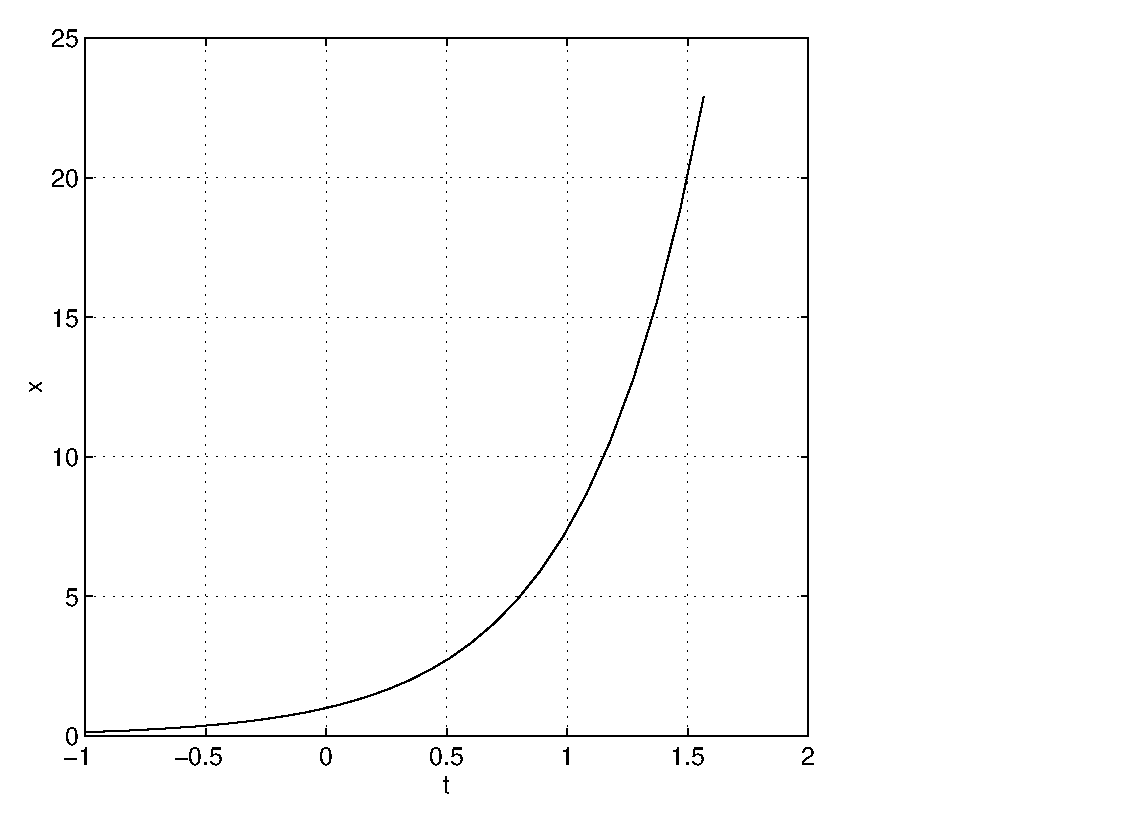
\psfig{file=figures/plotx.eps,height=2.0in,width=3.0in}
     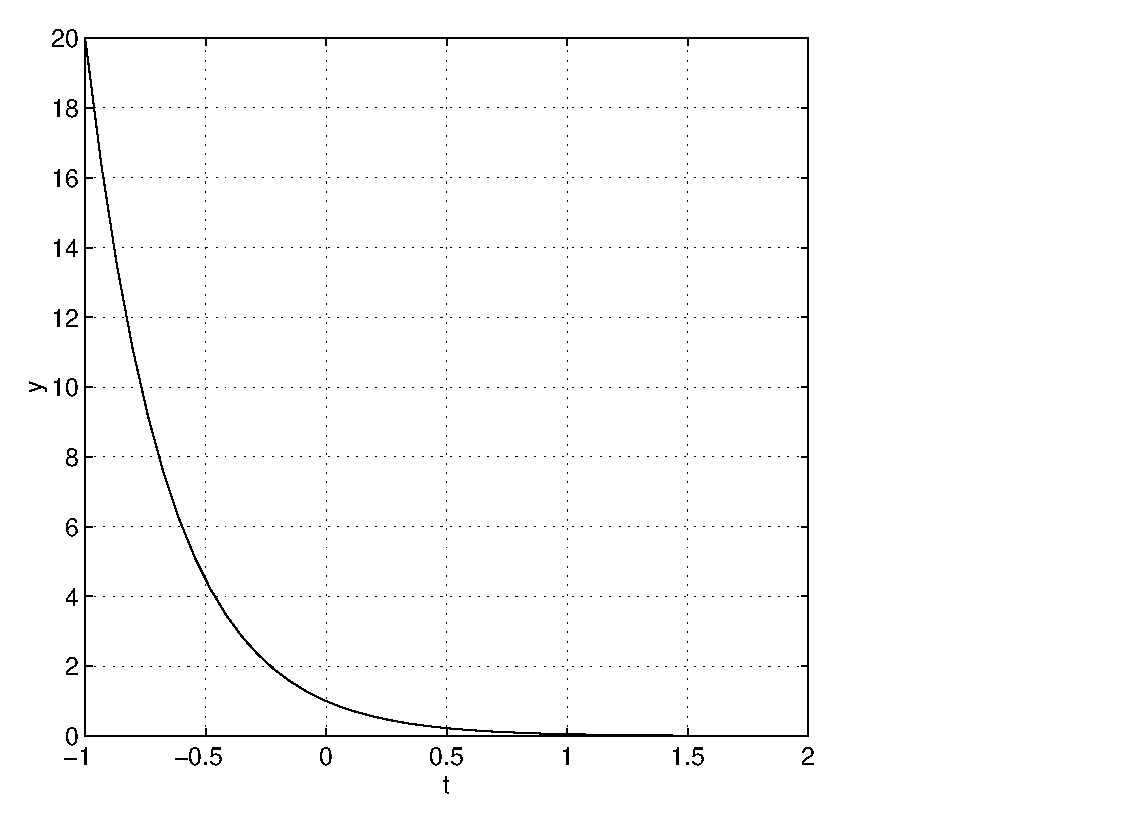
\psfig{file=figures/ploty.eps,height=2.0in,width=3.0in}}
     \centerline{%
     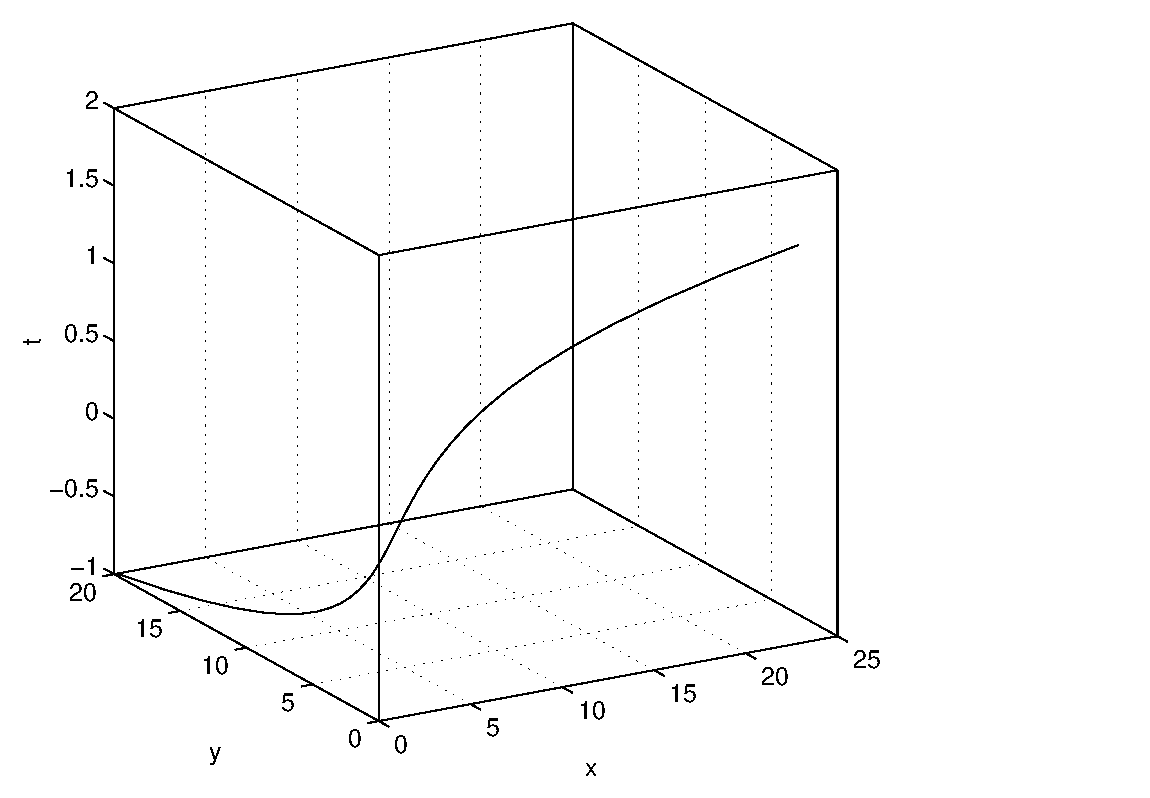
\psfig{file=figures/plot3d.eps,width=3.0in}
     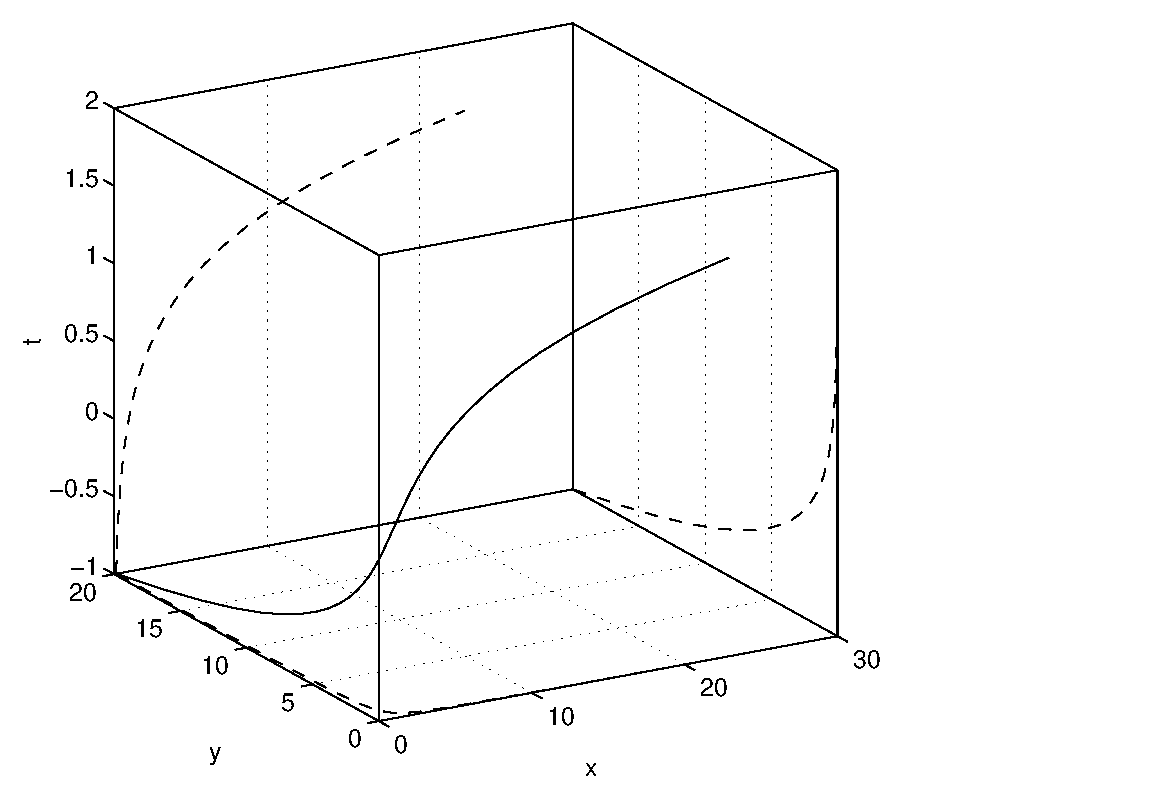
\psfig{file=figures/plotall.eps,width=3.0in}}
     \caption{{\sf PPLANE5 Display} for \protect\Ref{lin2} with
             $a=2$, $d=-3$ and $x\in [0,25], y\in [0,20]$. The solution
             going through $(1,1)$ is shown. UL: $(t,x(t))$;
	UR: $(t,y(t))$; LL: $(x(t),y(t),t)$; LR: all plots.}
     \label{plotall}
\end{figure}


\EXER

\TEXER

\noindent In Exercises~\ref{c3.5.1A} -- \ref{c3.5.1B} find all equilibria of
the given system of nonlinear autonomous differential equations.
\begin{exercise}  \label{c3.5.1A}
\begin{eqnarray*}
\dot{x} & = & x - y\\
\dot{y} & = & x^2 - y.
\end{eqnarray*}
\end{exercise}
\begin{exercise}  \label{c3.5.1B}
\begin{eqnarray*}
\dot{x} & = & x^2 - xy\\
\dot{y} & = & x^2 + y^2 - 4.
\end{eqnarray*}
\end{exercise}


\noindent In Exercises~\ref{E:uncoupleda} -- \ref{E:uncoupledc}
consider the uncoupled system of differential equations \Ref{lin2}.
For each choice of $a$ and $d$, determine whether the origin is a
saddle, source, or sink.
\begin{exercise} \label{E:uncoupleda}
$a=1$ and $d=-1$.
\end{exercise}
\begin{exercise} \label{E:uncoupledb}
$a=-0.01$ and $d=-2.4$.
\end{exercise}
\begin{exercise} \label{E:uncoupledc}
$a=0$ and $d=-2.3$.
\end{exercise}

\begin{exercise} \label{c3.4.2}
Let $(x(t),y(t))$ be the solution \Ref{e:explicitsoln} of \Ref{lin2}
with initial condition $(x(0),y(0))=(x_0,y_0)$, where $x_0\neq 0 \neq y_0$.
\begin{itemize}
\item[(a)] Show that the points $(x(t),y(t))$ lie on the curve whose 
equation is:
\[
y_0^ax^d - x_0^dy^a = 0.
\]
\item[(b)] Verify that if $a=1$ and $d=2$, then the solution lies
on a parabola tangent to the $x$-axis.
\end{itemize}
\end{exercise}

\begin{exercise} \label{c3.4.3}
Use the phase plane picture given in Figure~\ref{pp_dsp1} to
draw the time series $x(t)$ when $(x(0),y(0)) =
(\frac{1}{2},\frac{1}{2})$.  Check your answer using {\sf
pplane5}.
\end{exercise}

\CEXER


\begin{exercise} \label{c3.4.4}
For the three choices of $a$ and $d$ in the uncoupled system of
linear differential equations in Exercises~\ref{E:uncoupleda} -- 
\ref{E:uncoupledc}, use {\sf pplane5}
to compute phase portraits.  Use {\sf Keyboard input} to look at
solutions with initial conditions on the $x$ and $y$ axes.  As time
$t$ increases, do solutions with these initial conditions tend towards 
or away from the origin?
\end{exercise}

\begin{exercise} \label{c3.4.5}
Suppose that $a$ and $d$ are both negative, so that the origin
is asymptotically stable.  Make several choices of $a<d<0$ and
observe that solution trajectories tend to approach the origin
tangent to one of the axes.  Determine which one.  Try to prove
that your experimental guess is always correct?
\end{exercise}

\begin{exercise} \label{c3.4.6}
Suppose that $a=d<0$.  Verify experimentally using {\sf pplane5}
that all trajectories approach the origin along straight lines.
Try to prove this conjecture?
\end{exercise}

\begin{exercise} \label{c3.4.7}
Use {\sf pplane5} to compute several solutions of the linear system by
setting $a=2$ and $d=-3$ in the region $x,y\in[-5,5]$.  Then use
{\sf dfield5} to compute several solutions of the single differential
equation
\[
\frac{dx}{dt} = -\frac{2x}{3t}
\]
for $x,t\in[-5,5]$.  Is there a relationship between solutions to the
two equations and can you explain what that relationship is?
\end{exercise}



\section{Coupled Linear Systems} \index{coupled system} \label{s:3.5}


The general linear constant coefficient system in two unknown functions 
$x_1,x_2$ is:
\renewcommand{\arraystretch}{1.8}
\begin{equation}\label{lin3}
\begin{array}{ccc}
\dps \frac{dx_1}{dt}(t) & = & ax_1(t) + bx_2(t) \\
\dps \frac{dx_2}{dt}(t) & = & cx_1(t) + dx_2(t).
\end{array}
\end{equation}
\renewcommand{\arraystretch}{1.0}%
The uncoupled systems studied in Section~\ref{sec:UncoupledLS} are obtained 
by setting $b=c=0$ in \Ref{lin3}.  We have discussed how to solve \Ref{lin3} 
by formula \Ref{e:explicitsoln} when the system is uncoupled.  We have also 
discussed how to visualize the phase plane for different choices of the 
diagonal entries $a$ and $d$.  At present, we cannot
solve \Ref{lin3} by formula when the coefficient matrix is not diagonal.
But we may use {\sf pplane5} to solve the initial value problems numerically 
for these coupled systems.  We illustrate this point by solving
\begin{eqnarray*}
\frac{dx_1}{dt}(t) & = &  -x_1(t) + 3x_2(t) \\
\frac{dx_2}{dt}(t) & = &  3x_1(t) - x_2(t).
\end{eqnarray*}
After starting {\sf pplane5}, select {\sf linear system} from the
{\sf Gallery} and set the constants to:
\[
	a = -1,\quad b = 3,\quad c = 3, \quad d = -1.
\]
Click on {\sf Proceed}.  In order to have equally spaced coordinates on
the $x$ and $y$ axes, do the following.   In the {\sf PPLANE5 Display} 
window click on the {\sf edit} button and then on the {\sf zoom in square} 
command.  Then, using the mouse, click on the origin.

\subsection*{Eigendirections}

After computing several solutions, we find that for increasing
time $t$ all the solutions seem to approach the diagonal line
given by the equation $x_1=x_2$. Similarly, in backward time $t$
the solutions approach the anti-diagonal $x_1=-x_2$.  In other
words, as for the case of uncoupled systems, we find two
distinguished directions in the $(x,y)$-plane.  See
Figure~\ref{F:invariantlines}.  Moreover, the computations
indicate that these lines are invariant in the sense that
solutions starting on these lines remain on them for all time.
This statement can be verified numerically by using the {\sf
Keyboard input} in the {\sf PPLANE5 Options} to choose initial
conditions $(x_0,y_0)=(1,1)$ and $(x_0,y_0)=(1,-1)$.

\begin{figure}[htb]
     \centerline{%
     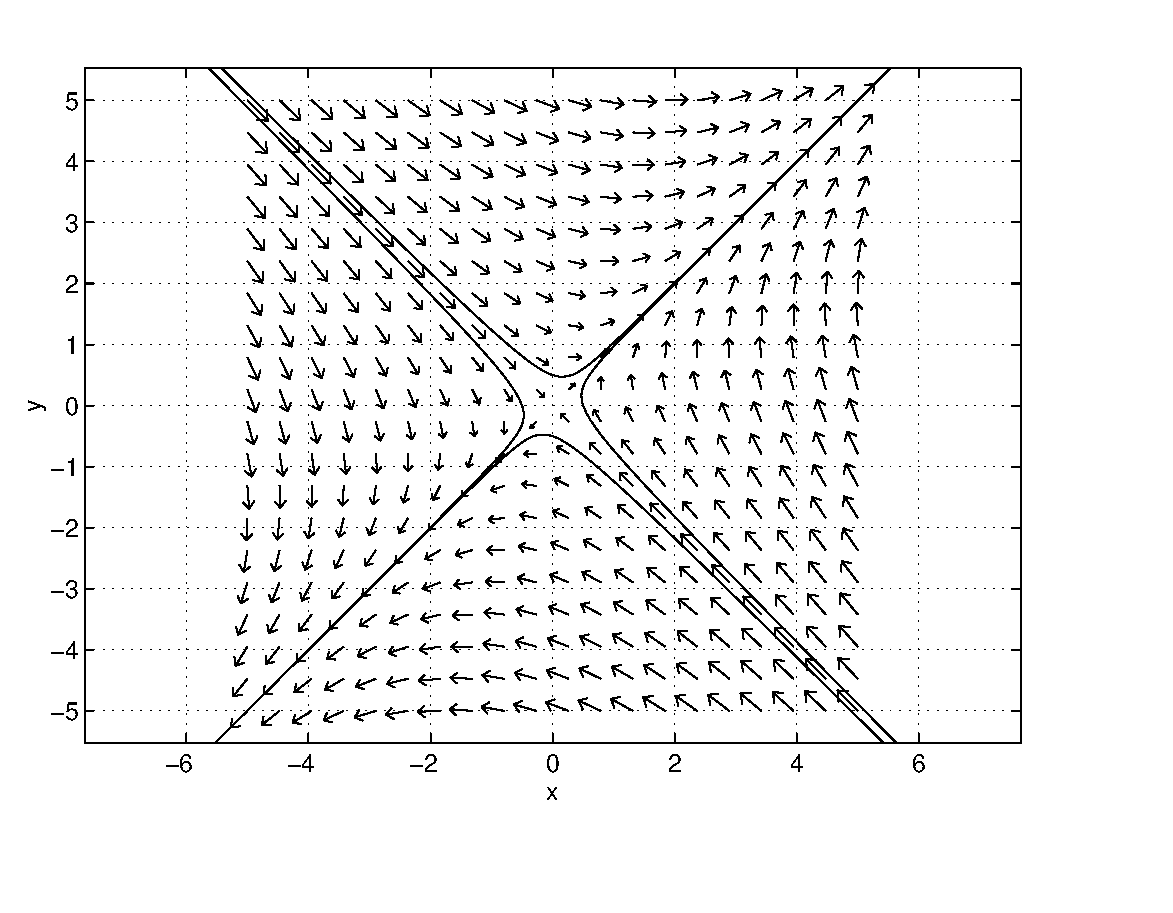
\psfig{file=figures/invline.eps,width=3.5in}}
     \caption{{\sf PPLANE5 Display} for \protect\Ref{lin3} with
             $a=-1=d$; $b=3=c$; and $x,y\in [-5,5]$.
	Solutions going through $(\pm 0.5,0)$ and $(0,\pm 0.5)$ are shown.}
     \label{F:invariantlines}
\end{figure}

\begin{Def} \label{D:eigendirection}
An invariant line for a linear system of differential equations
is called an {\em eigendirection}\index{eigendirection}.
\end{Def}

Observe that eigendirections vary if we change parameters.  For
example, if we set $b$ to $1$, then there are still two
distinguished lines but these lines are no longer perpendicular.

For uncoupled systems, we have shown analytically that the $x$
and $y$ axes are eigendirections.  The numerical computations
that we have just performed indicate that eigendirections exist
for many coupled systems.  This discussion leads naturally to
two questions:
\begin{enumerate}
\item Do eigendirections always exist?
\item How can we find eigendirections?
\end{enumerate}
The second question will be answered in Sections~\ref{S:IVP&E} and 
\ref{S:evchp}.  We can answer the first question by performing another 
numerical computation.  In the setup window, change the parameter $b$ 
to $-2$.  Then numerically compute some solutions to see that there
are no eigendirections in the phase space of this system.  Observe that
all solutions appear to spiral into the origin as time goes to
infinity.  The phase portrait is shown in Figure~\ref{pp_dsp2}.
\begin{figure}[htb]
      \centerline{%
      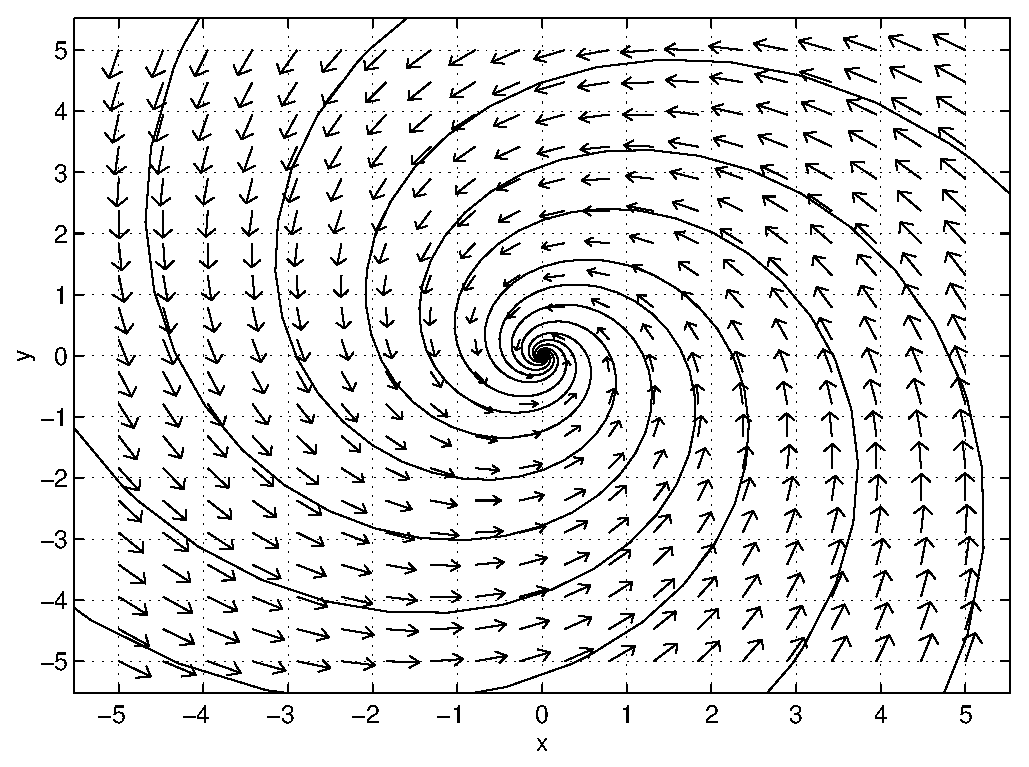
\psfig{file=figures/pp_dsp2.eps,width=3.5in}}
      \caption{{\sf PPLANE5 Display} for the {\sf linear system}
		with $a=-1$, $b=-2$, $c=3$, $d=-1$.}
      \label{pp_dsp2}
\end{figure}

\subsubsection*{Second Order Differential Equations}
\index{differential equation!second order}

We now show analytically that certain linear systems of
differential equations have no invariant lines in their phase portrait.

We do this by showing that second order differential equations can be
reduced to first order systems by a simple but important trick.  Indeed,
sometimes it is easier to solve a single second order equation, and
sometimes it is easier to solve the first order system.  At this stage
we introduce this connection by considering the differential equation
\begin{equation}  \label{E:2ndordera}
\frac{d^2x}{dt^2} + x = 0.
\end{equation}
This differential equation states that we are looking for a function
$x(t)$ whose second derivative is $-x(t)$.  From calculus, we know
that $x(t)=\cos t$ is such a function.

Let $y(t)=\dot{x}(t)$.  Then
\Ref{E:2ndordera} may be rewritten as a first order coupled system
in $x(t)$ and $y(t)$ as follows:
\begin{equation}  \label{E:2nd->1st}
\begin{array}{rcl}
\dot{x} & = & y \\
\dot{y} & = & -x.
\end{array}
\end{equation}
Observe that if $x(t)$ is a solution to \Ref{E:2ndordera}, then
\[
0 = \frac{d^2x}{dt^2} + x = \frac{dy}{dt} + x.
\]
Hence,
\[
\dot{y} = -x
\]
Conversely, if $(x(t),y(t))$ is a solution to \Ref{E:2nd->1st}, then
$x(t)$ is a solution to \Ref{E:2ndordera}.  That is,
\[
\frac{d^2x}{dt^2} + x = \frac{dy}{dt} + x = -x + x = 0.
\]

It follows from the discussion that $(x(t),y(t))=(\cos t,\sin t)$ is 
a solution to the differential equation \Ref{E:2nd->1st}.  We have shown 
analytically that the unit circle centered at the origin is a solution 
trajectory for \Ref{E:2nd->1st}.  Hence \Ref{E:2nd->1st} has no 
eigendirections.  It may be checked using \Matlab that all solution 
trajectories for \Ref{E:2nd->1st} are just circles centered at the origin.


\EXER

\CEXER

\begin{exercise} \label{c3.5.a01}
Choose the {\sf linear system} in {\sf pplane5} and set $a=0$, $b=1$, and 
$c=-1$.  Then find values $d$ such that except for the origin itself all 
solutions appear to
\begin{itemize}
\item[(a)] spiral into the origin;
\item[(b)] spiral away from the origin;
\item[(c)] form circles around the origin;
\end{itemize}
\end{exercise}

\begin{exercise} \label{c3.5.2}
Choose the {\sf linear system} in {\sf pplane5} and set
$a=-1$, $c=3$, and $d=-1$.
Then find a value for $b$ such that the behavior of the
solutions of the system is ``qualitatively'' the same as for a
diagonal system where $a$ and $d$ are negative.  In particular,
the origin should be an asymptotically stable equilibrium and
the solutions should approach that equilibrium along a
distinguished line.
\end{exercise}

\begin{exercise} \label{c3.5.3}
Choose the {\sf linear system} in {\sf pplane5} and set
$a=d$ and $b=c$.  Verify that for these systems of differential
equations:
\begin{itemize}
\item[(a)]  When $|a|<b$ typical trajectories approach the line
$y=x$ as $t\to\infty$ and the line $y=-x$ as $t\to -\infty$.
\item[(b)]  Assume that $b$ is positive, $a$ is negative, and $b<-a$. 
With these assumptions show that the origin is a sink and that typical 
trajectories approach the origin tangent to the line $y=x$.
\end{itemize}
\end{exercise}

\TEXER

\begin{exercise} \label{c3.5.4}
Sketch the time series $y(t)$ for the solution to the
differential equation whose phase plane is pictured in
Figure~\ref{pp_dsp2} with initial condition
$(x(0),y(0))=(\frac{1}{2},\frac{1}{2})$ .  Check your answer
using {\sf pplane5}.
\end{exercise}

\noindent In Exercises~\ref{c3.5.5a} -- \ref{c3.5.5d}, determine which of
the function pairs $(x_1(t),y_1(t))$ and $(x_2(t),y_2(t))$ are solutions
to the given system of ordinary differential equations.
\begin{exercise} \label{c3.5.5a}
The ODE is:
\begin{eqnarray*}
\dot{x} & = & 2x+y  \\
\dot{y} & = & 3y.
\end{eqnarray*}
The pairs of functions are:
\[
(x_1(t),y_1(t)) = (e^{2t},0)  \AND (x_2(t),y_2(t)) = (e^{3t},e^{3t}).
\]
\end{exercise}
\begin{exercise} \label{c3.5.5b}
The ODE is:
\begin{eqnarray*}
\dot{x} & = & 2x - 3y  \\
\dot{y} & = & x - 2y.
\end{eqnarray*}
The pairs of functions are:
\[
(x_1(t),y_1(t)) = e^t(3,1)  \AND (x_2(t),y_2(t)) = (e^{-t},e^{-t}).
\]
\end{exercise}
\begin{exercise} \label{c3.5.5c}
The ODE is:
\begin{eqnarray*}
\dot{x} & = &  x + y \\
\dot{y} & = & -x + y.
\end{eqnarray*}
The pairs of functions are:
\[
(x_1(t),y_1(t)) =  (3e^t, -2e^t) \AND (x_2(t),y_2(t)) = e^t(\sin t,\cos t).
\]
\end{exercise}
\begin{exercise} \label{c3.5.5d}
The ODE is:
\begin{eqnarray*}
\dot{x} & = & y  \\
\dot{y} & = &  -\frac{1}{t^2}x + \frac{1}{t}y + 1.
\end{eqnarray*}
The pairs of functions are:
\[
(x_1(t),y_1(t)) = (t^2,2t)  \AND (x_2(t),y_2(t)) = (2t^2,4t).
\]
\end{exercise}


\section{The Initial Value Problem and Eigenvectors}
\label{S:IVP&E} \index{initial value problem}

The general {\em constant coefficient\/}
\index{system of differential equations!constant coefficient}
system of differential equations has the form
\renewcommand{\arraystretch}{1.8}
\begin{equation}\label{lingen}
\begin{array}{ccc}
\dps \frac{dx_1}{dt}(t) & = & c_{11}x_1(t) + \cdots + c_{1n}x_n(t) \\
\vdots  & \vdots & \vdots \\
\dps \frac{dx_n}{dt}(t) & = & c_{n1}x_1(t) + \cdots + c_{nn}x_n(t)
\end{array}
\end{equation}
\renewcommand{\arraystretch}{1.0}%
where the coefficients $c_{ij}\in \R$ are constants.  Suppose that 
\Ref{lingen} satisfies the initial conditions $x_1(0) = K_1$, \ldots,  
$x_n(0) = K_n$.

Using matrix multiplication of a vector and matrix, we can rewrite these 
differential equations in a compact form.   Consider the $n\times n$ 
coefficient matrix
\[
C = \left(
\begin{array}{rrrr}
 c_{11} & c_{12} & \cdots & c_{1n} \\
 c_{21} & c_{22} & \cdots & c_{2n}  \\
 \vdots & \vdots &        & \vdots  \\
 c_{n1} & c_{n2} & \cdots & c_{nn}
\end{array}
\right)
\]
and the $n$ vectors of initial conditions and unknowns
\[
X_0=\left(
\begin{array}{ccc}
K_1 \\ \vdots  \\ K_n
\end{array}
\right) \AND
X=\left(
\begin{array}{ccc}
x_1 \\ \vdots  \\ x_n
\end{array}
\right).
\]
Then \Ref{lingen} has the compact form
\begin{equation}  \label{E:geneqn}
\begin{array}{rcl}
\dps\frac{dX}{dt} & = & CX\\
X(0) & = & X_0.  
\end{array}
\end{equation}


In Section~\ref{s:3.5}, we plotted the phase space picture 
of the planar system of differential equations
\begin{equation} \label{-13}
\vectwo{\dot{x}}{\dot{y}}
= C \vectwo{x(t)}{y(t)}
\end{equation}
where
\[
C = \mattwo{-1}{3}{3}{-1}.
\]
In those calculations we observed that there is a solution to
\Ref{-13} that stayed on the main diagonal for each moment in
time.  Note that a vector is on the main diagonal if it is a
scalar multiple of $\vectwo{1}{1}$.  Thus a solution that stays
on the main diagonal for all time $t$ must have the form
\begin{equation} \label{e:diagform}
\vectwo{x(t)}{y(t)} = u(t) \vectwo{1}{1}
\end{equation}
for some real-valued function $u(t)$.  When a function of form
\Ref{e:diagform} is a solution to \Ref{-13}, it satisfies:
\[
\dot{u}(t)\vectwo{1}{1} = \vectwo{\dot{x}(t)}{\dot{y}(t)} =
C \vectwo{x(t)}{y(t)} = C u(t)\vectwo{1}{1} = u(t) C \vectwo{1}{1}.
\]
A calculation shows that
\[
C \vectwo{1}{1} = 2 \vectwo{1}{1}.
\]
Hence
\[
\dot{u}(t) \vectwo{1}{1} =  2 u(t) \vectwo{1}{1}.
\]
It follows that the function $u(t)$ must satisfy the
differential equation
\[
\frac{du}{dt} = 2u.
\]
whose solutions are
\[
u(t) = \alpha e^{2t},
\]
for some scalar $\alpha$.

Similarly, we also saw in our \Matlab experiments that there was
a solution that for all time stayed on the anti-diagonal, the
line $y=-x$.  Such a solution must have the form
\[
\vectwo{x(t)}{y(t)} = v(t) \vectwo{1}{-1}.
\]
A similar calculation shows that $v(t)$ must satisfy the
differential equation
\[
\frac{dv}{dt} = -4v.
\]
Solutions to this equation all have the form
\[
v(t) = \beta e^{-4t},
\]
for some real constant $\beta$.

Thus, using matrix multiplication, we are able to prove
analytically that there are solutions to \Ref{-13} of exactly
the type suggested by our \Matlab experiments.  However, even
more is true and this extension is based on the principle of 
superposition that was introduced for algebraic equations in 
Section~\ref{S:Superposition}.  

\subsection*{Superposition in Linear Differential Equations}
\index{superposition}\index{differential equation!superposition}

Consider a general linear differential equation of the form
\begin{equation} \label{gen1}
\frac{dX}{dt} = CX,
\end{equation}
where $C$ is an $n\times n$ matrix.  Suppose that $Y(t)$ and
$Z(t)$ are solutions to \Ref{gen1} and $\alpha,\beta\in\R$ are
scalars.  Then $X(t)=\alpha Y(t)+\beta Z(t)$ is also a solution.
We verify this fact using the `linearity' of $d/dt$.  Calculate
\begin{eqnarray*}
\frac{d}{dt} X(t) & = &
\alpha \frac{dY}{dt}(t) + \beta \frac{dZ}{dt}(t) \\
 & = &\alpha CY(t) + \beta CZ(t)\\
 & = & C(\alpha Y(t) + \beta Z(t))\\
 & = & CX(t).
\end{eqnarray*}
So superposition is valid for solutions of linear differential equations.


\subsection*{Initial Value Problems}
\index{initial value problem}

Suppose that we wish to find a solution to
\Ref{-13} satisfying the initial conditions\index{initial condition}
\[
\left(\begin{array}{c} x(0) \\ y(0) \end{array}\right) =
\left(\begin{array}{c}1\\3\end{array}\right).
\]
Then we can use the principle of superposition to find this solution in 
closed form.  Superposition implies that for each pair of scalars 
$\alpha,\beta\in\R$, the functions
\begin{equation}  \label{e:solnODE}
\left(\begin{array}{c} x(t) \\ y(t) \end{array}\right) =
\alpha e^{2t}\left(\begin{array}{c}1\\1\end{array}\right) +
\beta e^{-4t}\left(\begin{array}{r} 1\\-1\end{array}\right),
\end{equation}
are solutions to \Ref{-13}.  Moreover, for a solution of this form 
\[
\left(\begin{array}{c} x(0) \\ y(0) \end{array}\right) =
\left(\begin{array}{c} \alpha+\beta \\ \alpha-\beta
\end{array}\right).
\]

Thus we can solve our prescribed initial value problem, if we can
solve the system of linear equations
\begin{eqnarray*}
\alpha + \beta = 1\ \\
\alpha - \beta = 3.
\end{eqnarray*}
This system is solved for $\alpha=2$ and $\beta=-1$. Thus
\[
\vectwo{x(t)}{y(t)} = 2e^{2t}\vectwo{1}{1} - e^{-4t}\vectwo{1}{-1}
\]
is the desired closed form solution.

\subsection*{Eigenvectors and Eigenvalues}

We emphasize that just knowing that there are two lines in the
plane that are invariant under the dynamics of the system of
linear differential equations is sufficient information to solve
these equations.  So it seems appropriate to ask the question:
When is there a line that is invariant under the dynamics of a
system of linear differential equations?  This question is
equivalent to asking:  When is there a nonzero vector $v$ and a
nonzero real-valued function $u(t)$ such that
\[
X(t) = u(t) v
\]
is a solution to \Ref{gen1}?

Suppose that $X(t)$ is a solution to the system of differential
equations $\dot{X}=CX$.  Then $u(t)$ and $v$ must satisfy
\begin{equation}  \label{E:diffdir}
\dot{u}(t)v = \frac{dX}{dt} = CX(t) = u(t) Cv.
\end{equation}
Since $u$ is nonzero, it follows that $v$ and $Cv$ must lie on the
same line through the origin.  Hence
\begin{equation}  \label{e:eigendef}
Cv = \lambda v,
\end{equation}
for some real number $\lambda$.

\begin{Def}  \label{D:eigenvalue1}
A nonzero vector $v$ satisfying \Ref{e:eigendef} is called an
{\em eigenvector\/} \index{eigenvector} of the matrix $C$, and
the number $\lambda$ is an {\em eigenvalue\/} \index{eigenvalue}
of the matrix $C$.
\end{Def}
Geometrically, the matrix $C$ maps an eigenvector onto a multiple
of itself --- that multiple is the eigenvalue.

Note that scalar multiples of eigenvectors are also eigenvectors.  More 
precisely:
\begin{lemma}  \label{L:e'vector}
Let $v$ be an eigenvector of the matrix $C$ with eigenvalue $\lambda$.   
Then $\alpha v$ is also an eigenvector of $C$ with eigenvalue $\lambda$ 
as long as $\alpha\neq 0$.
\end{lemma}

\begin{proof} By assumption, $Cv=\lambda v$ and $v$ is nonzero. Now calculate
\[
C(\alpha v) = \alpha Cv = \alpha\lambda v = \lambda(\alpha v).
\]
The lemma follows from the definition of eigenvector.  \end{proof}

It follows from \Ref{E:diffdir} and \Ref{e:eigendef} that if $v$ is
an eigenvector of $C$ with eigenvalue $\lambda$, then
\[
\frac{du}{dt} = \lambda u.
\]
Thus we have returned to our original linear differential
equation that has solutions
\[
u(t) = Ke^{\lambda t},
\]
for all constants $K$.

We have proved the following theorem.
\begin{thm}  \label{T:eigensoln}
Let $v$ be an eigenvector of the $n\times n$ matrix $C$ with
eigenvalue $\lambda$.  Then
\[
X(t) = e^{\lambda t}v
\]
is a solution to the system of differential equations $\dot{X}=CX$.
\end{thm}



Finding eigenvalues and eigenvectors from first principles --- even for 
$2\times 2$ matrices --- is not a simple task.  We end this section with 
a calculation illustrating that real eigenvalues need not exist.  In 
Section~\ref{S:evchp}, we present a natural method for computing  
eigenvalues (and eigenvectors) of $2\times2$ matrices.  We defer the 
discuss of how to find eigenvalues and eigenvectors of $n\times n$ matrices 
until Chapter~\ref{C:D&E}.


\subsubsection*{An Example of a Matrix with No Real Eigenvalues}

Not every matrix has {\em real\/} eigenvalues\index{eigenvalue!real} and
eigenvectors\index{eigenvector!real}.  Recall the linear system of differential 
equations $\dot{x}=Cx$ whose phase plane is pictured in Figure~\ref{pp_dsp2}.  
That phase plane showed no evidence of an invariant line and indeed there is 
none.  The matrix $C$ in that example was
\[
C=\mattwo{-1}{-2}{3}{-1}.
\]
We ask: Is there a value of $\lambda$ and a nonzero vector
$(x,y)$ such that
\begin{equation}  \label{E:eigexamp}
C\left(\begin{array}{c} x\\y\end{array}\right) =
\lambda  \left(\begin{array}{c} x\\y\end{array}\right)?
\end{equation}
Equation \Ref{E:eigexamp} implies that
\[
\left(\begin{array}{cc} -1-\lambda & -2 \\ 3 & -1-\lambda
\end{array}\right) \left(\begin{array}{c}
x\\y\end{array}\right) =0.
\]
If this matrix is row equivalent to the identity matrix, then
the only solution of the linear system is $x=y=0$.  To have a
nonzero solution, the matrix
\[
\left(\begin{array}{cc} -1-\lambda & -2 \\ 3 & -1-\lambda
\end{array}\right)
\]
must not be row equivalent to $I_2$.  Dividing the $1^{st}$ row by
$-(1+\lambda)$ leads to
\[
\left(\begin{array}{cc} 1 & \frac{2}{1+\lambda} \\ 3 & -1-\lambda
\end{array}\right).
\]
Subtracting $3$ times the $1^{st}$ row from the second produces
the matrix
\[
\left(\begin{array}{cc} 1 & \frac{2}{1+\lambda} \\ 0 &
-(1+\lambda) - \frac{6}{1+\lambda}
\end{array}\right).
\]
This matrix is not row equivalent to $I_2$ when the lower
right hand entry is zero; that is, when
\[
(1+\lambda) +\frac{6}{1+\lambda} = 0.
\]
That is, when
\[
(1+\lambda)^2 = -6,
\]
which is not possible for any real number $\lambda$.  This
example shows that the question of whether a given matrix has a
real eigenvalue and a real eigenvector --- and hence when the
associated system of differential equations has a line that is
invariant under the dynamics --- is a subtle question.

Questions concerning eigenvectors and eigenvalues are central to
much of the theory of linear algebra.  We discuss this
topic for $2\times 2$ matrices in Section~\ref{S:evchp} and
Chapter~\ref{Chap:Planar} and for general square matrices in
Chapters~\ref{C:D&E} and \ref{C:HDeigenvalues}.

\EXER

\TEXER

\begin{exercise} \label{c4.1.5}
Write the system of linear ordinary differential equations
\begin{eqnarray*}
\frac{dx_1}{dt}(t) & = & 4x_1(t) + 5x_2(t) \\
\frac{dx_2}{dt}(t) & = & 2x_1(t) - 3x_2(t)
\end{eqnarray*}
in matrix form.
\end{exercise}

\begin{exercise} \label{c4.4.4}
Show that all solutions to the system of linear differential equations
\begin{eqnarray*}
\frac{dx}{dt} & = & 3x \\
\frac{dy}{dt} & = & -2y
\end{eqnarray*}
are linear combinations of the two solutions
\[
U(t) = e^{3t}\vectwo{1}{0} \AND V(t) = e^{-2t}\vectwo{0}{1}.
\]
\end{exercise}

\begin{exercise} \label{c4.5.1}
Consider
\begin{equation}  \label{e:Ceqn}
\frac{dX}{dt}(t) = CX(t)
\end{equation}
where
\[
C=\left(\begin{array}{cr} 2 & 3\\0& -1 \end{array}\right).
\]
Let
\[
v_1=\left(\begin{array}{c} 1\\0\end{array}\right)\AND
v_2=\left(\begin{array}{r} 1\\-1\end{array}\right),
\]
and let
\[
Y(t)=e^{2t} v_1 \AND Z(t)=e^{-t}v_2.
\]
\begin{itemize}
\item[(a)] Show that $Y(t)$ and $Z(t)$ are solutions to \Ref{e:Ceqn}.
\item[(b)] Show that $X(t)=2Y(t)-14Z(t)$ is a solution to \Ref{e:Ceqn}.
\item[(c)] Use the principle of superposition to verify that
$X(t)=\alpha Y(t) + \beta Z(t)$ is a solution to \Ref{e:Ceqn}.
\item[(d)] Using the general solution found in part (c), find a solution
$X(t)$ to \Ref{e:Ceqn} such that
\[
X(0) = \left(\begin{array}{r} 3\\-1\end{array}\right).
\]
\end{itemize}
\end{exercise}

\begin{exercise} \label{c4.5.2}
Find a solution to
\[
\dot{X}(t)=CX(t)
\]
where
\[
C=\mattwo{1}{-1}{-1}{1}
\]
and
\[
X(0)=\vectwo{2}{1}.
\]
{\bf Hint:} Observe that
\[
\vectwo{1}{1} \AND \vectwo{1}{-1}
\]
are eigenvectors of $C$.
\end{exercise}

\begin{exercise} \label{c4.5.3}
Let
\[
C=\mattwo{a}{b}{b}{a}.
\]
Show that
\[
\vectwo{1}{1} \AND \vectwo{1}{-1}
\]
are eigenvectors of $C$.  What are the corresponding eigenvalues?
\end{exercise}

\begin{exercise} \label{c4.5.4}
Let
\[
C=\mattwo{1}{2}{-3}{-1}.
\]
Show that $C$ has no real eigenvectors.
\end{exercise}

\begin{exercise}  \label{c4.9.6A}
Suppose that $A$ is an $n\times n$ matrix with zero as an eigenvalue.
Show that $A$ is not invertible.  {\bf Hint:}  Assume that $A$ is invertible 
and compute $A\inv Av$ where $v$ is an eigenvector of $A$ corresponding to 
the zero eigenvalue.
\end{exercise}
\noindent {\bf Remark:}  In fact, $A$ is invertible\index{invertible} if 
all of the eigenvalues of $A$ are nonzero.  See Corollary~\ref{C:eig=0} of 
Chapter~\ref{C:D&E}.


\CEXER

\begin{exercise} \label{c4.5.6}
Consider the matrix $A$ and vector $X_0$ given by
\[
A=\mattwo{2}{1}{0}{1}\AND X_0=\vectwo{1}{1}.
\]
Use {\sf map} to compute $X_1 = AX_0$, $X_2 = AX_1$, $X_3=AX_2$ etc.\ by a
repeated use of the {\sf Map} button in the {\sf MAP Display} window.  What
do you observe?  What happens if you start the iteration process with a
different choice for $X_0$, and, in particular, for an $X_0$ that is close
to $\vectwo{-1}{1}$?
\end{exercise}

\noindent In Exercises~\ref{c4.5.5a} -- \ref{c4.5.5b} use {\sf map} to find
an (approximate) eigenvector for the given matrix.  {\bf Hint:} Choose a
vector in {\sf map} and repeatedly click on the button {\sf Map} until the
vector maps to a multiple of itself.  You may wish to use the {\sf Rescale} 
feature in the {\sf MAP Options}.  Then the length of the vector is rescaled 
to one after each use of the command {\sf Map}. In this way, you can avoid
overflows in the computations while still being able to see the
directions where the vectors are moved by the matrix mapping.  The coordinates 
of the new vector obtained by applying {\sf map} can be viewed in the 
{\sf Vector input} window.

\begin{exercise} \label{c4.5.5a}
$B=\mattwo{2}{-2}{2}{7}$.
\end{exercise}
\begin{exercise} \label{c4.5.5b}
$C=\mattwo{1}{1.5}{0}{-2}$.
\end{exercise}

\begin{exercise} \label{c4.4.5}
Use \Matlab to verify that solutions to the system of linear differential
equations
\begin{eqnarray*}
\frac{dx}{dt} & = & 2x + y\\
\frac{dy}{dt} & = & y
\end{eqnarray*}
are linear combinations of the two solutions
\[
U(t) = e^{2t}\vectwo{1}{0} \AND V(t) = e^{t}\vectwo{-1}{1}.
\]
More concretely, proceed as follows:
\begin{itemize}
\item[(a)]  By superposition, the general solution to the differential
equation has the form $X(t)=\alpha U(t) + \beta V(t)$.  Find constants
$\alpha$ and $\beta$ such that $\alpha U(0) + \beta V(0) = \vectwo{0}{1}$.
\item[(b)] Graph the second component $y(t)$ of this solution using the
\Matlab {\tt plot} command.
\item[(c)] Use {\sf pplane5} to compute a solution via the {\sf Keyboard
input} starting at $(x(0),y(0)) = (0,1)$ and then use the
{\tt y} {\tt vs} {\tt t} command in {\sf pplane5} to graph this solution.
\item[(d)] Compare the results of the two plots.
\item[(e)]  Repeat steps (a)--(d) using the initial vector $\vectwo{1}{1}$.
\end{itemize}
\end{exercise}


\section{Eigenvalues of $2\times 2$ Matrices}
\label{S:evchp}


We now discuss how to find eigenvalues
\index{eigenvalue} of $2\times 2$ matrices in a way that does
not depend explicitly on finding eigenvectors.
\index{eigenvector} This direct method will show that
eigenvalues can be complex as well as real.

We begin the discussion with a general square matrix.  Let $A$
be an $n\times n$ matrix.  Recall that $\lambda\in\R$ is an
eigenvalue of $A$ if there is a nonzero vector $v\in\R^n$ for
which
\begin{equation}  \label{eigeneqn}
Av = \lambda v.
\end{equation}
The vector $v$ is called an eigenvector.  We may rewrite
\Ref{eigeneqn} as:
\[
(A-\lambda I_n)v = 0.
\]
Since $v$ is nonzero, it follows that if $\lambda$ is an
eigenvalue of $A$, then the matrix $A-\lambda I_n$ is singular.

Conversely, suppose that $A-\lambda I_n$ is singular for some
real number $\lambda$.  Then Theorem~\ref{invertequiv} of 
Chapter~\ref{chap:matrices} implies that there is a nonzero
vector $v\in\R^n$ such that $(A-\lambda I_n)v = 0$. Hence
\Ref{eigeneqn} holds and $\lambda$ is an eigenvalue of $A$.
So, if we had a direct method for determining when a matrix
is singular, then we would have a method for determining
eigenvalues.

\subsubsection*{Characteristic Polynomials}

Corollary~\ref{C:2x2invert} of Chapter~\ref{chap:matrices}
states that $2\times 2$ matrices are singular precisely when
their determinant is zero.  It follows that $\lambda\in\R$ is
an eigenvalue for the $2\times 2$ matrix $A$ precisely when
\begin{equation} \label{deteqn}
\det(A-\lambda I_2) = 0.
\end{equation}
We can compute \Ref{deteqn} explicitly as follows. Note that
\[
A-\lambda I_2 = \left(\begin{array}{cc} a-\lambda & b \\
c & d-\lambda \end{array} \right).
\]
Therefore
\begin{eqnarray}
\det(A-\lambda I_2) & = & (a-\lambda)(d-\lambda) - bc \nonumber \\
& = & \lambda^2 - (a+d)\lambda + (ad-bc). \label{e:charpoly}
\end{eqnarray}

\begin{Def} \label{charpolyn=2}
The {\em characteristic polynomial\/} of the matrix $A$ is
\[
p_A(\lambda) = \det(A-\lambda I_2).
\]
\end{Def} \index{characteristic polynomial}

For an $n\times n$ matrix $A=(a_{ij})$, define the {\em trace\/}
\index{trace} of $A$ to be the sum of the diagonal elements of $A$;
that is
\begin{equation}  \label{e:tracedef}
{\rm tr}(A) = a_{11} + \cdots + a_{nn}.
\end{equation}
Thus, using \Ref{e:charpoly}, we can rewrite the characteristic
polynomial for $2\times 2$ matrices as
\begin{equation} \label{e:invcharpoly}
p_A(\lambda)=\lambda^2 - {\rm tr}(A)\lambda + \det(A).
\end{equation}

As an example, consider the $2\times 2$ matrix
\begin{equation} \label{e:2x2ex}
A=\mattwo{2}{3}{1}{4}.
\end{equation}
Then
\[
A-\lambda I_2 = \left(\begin{array}{cc} 2-\lambda & 3 \\
1 & 4-\lambda \end{array}\right),
\]
and
\[
p_A(\lambda) = (2-\lambda)(4-\lambda)-3 = \lambda^2-6\lambda+5.
\]
It is now easy to verify \Ref{e:invcharpoly} for \Ref{e:2x2ex}.

\subsubsection*{Eigenvalues}

For $2\times 2$ matrices $A$, $p_A(\lambda)$ is a quadratic
polynomial.  As we have discussed, the real roots of $p_A$ are
real eigenvalues of $A$.  For $2\times 2$ matrices we now 
generalize our first definition of eigenvalues, 
Definition~\ref{D:eigenvalue1}, to include complex eigenvalues, as follows.

\begin{Def}
An {\em eigenvalue\/} of $A$ is a root of the characteristic polynomial $p_A$.
\end{Def} \index{eigenvalue} \index{characteristic polynomial}
Suppose that $\lambda_1$ and $\lambda_2$ are the roots of $p_A$.
It follows that
\begin{equation}  \label{e:charpolyprod}
p_A(\lambda) = (\lambda-\lambda_1)(\lambda-\lambda_2) =
\lambda^2 - (\lambda_1+\lambda_2)\lambda + \lambda_1\lambda_2.
\end{equation}
Equating the two forms of $p_A$ \Ref{e:invcharpoly} and
\Ref{e:charpolyprod} shows that
\begin{eqnarray}
\trace(A) & = & \lambda_1 + \lambda_2 \label{e:treigen}\\
\det(A) & = & \lambda_1\lambda_2. \label{e:deteigen}
\end{eqnarray}
Thus, for $2\times 2$ matrices, the trace is the sum of the
eigenvalues and the determinant is the product of the eigenvalues.
In Chapter~\ref{C:D&E}, Theorems~\ref{T:eigens}(b) and
\ref{T:tracen} we show that these statements are also valid for
$n\times n$ matrices.

Recall that in example \Ref{e:2x2ex} the characteristic polynomial
is
\[
p_A(\lambda) = \lambda^2-6\lambda+5=(\lambda-5)(\lambda-1).
\]
Thus the eigenvalues of $A$ are $\lambda_1=1$ and $\lambda_2=5$
and identities \Ref{e:treigen} and \Ref{e:deteigen} are easily
verified for this example.  

Next, we consider an example with complex eigenvalues and verify that these 
identities are equally valid in this instance.  Let
\[
B = \mattwo{2}{-3}{1}{4}.
\]
The characteristic polynomial is:
\[
p_B(\lambda) = \lambda^2 -6\lambda + 11.
\]
Using the quadratic formula we see that the roots of $p_B$ (that
is, the eigenvalues of $B$) are
\[
\lambda_1 = 3 + i\sqrt{2} \AND \lambda_2 = 3 -i\sqrt{2}.
\]
Again the sum of the eigenvalues is $6$ which equals the trace
of $B$ and the product of the eigenvalues is $11$ which equals
the determinant of $B$.

Since the characteristic polynomial of $2\times 2$ matrices is
always a quadratic polynomial, it follows that $2\times 2$
matrices have precisely two eigenvalues --- including
multiplicity --- and these can be described as follows.  The
{\em discriminant\/}\index{discriminant} of $A$ is:
\begin{equation}  \label{e:discriminant}
D = [\trace(A)]^2 -4\det(A).
\end{equation}
\begin{thm} \label{eigendist}
There are three possibilities for the two eigenvalues of a
$2\times 2$ matrix $A$ that we can describe in terms of the
discriminant:
\begin{itemize}
\item[(i)] The eigenvalues of $A$ are real and distinct ($D>0$).
\item[(ii)] The eigenvalues of $A$ are a complex conjugate pair ($D<0$).
\item[(iii)] The eigenvalues of $A$ are real and equal ($D=0$).
\end{itemize}
\end{thm} \index{eigenvalue}

\begin{proof} We can find the roots of the characteristic polynomial
using the form of $p_A$ given in \Ref{e:invcharpoly} and the
quadratic formula.  The roots are:
\[
\frac{1}{2}\left({\rm tr}(A)\pm \sqrt{[{\rm tr}(A)]^2-4\det(A)}\right)
= \frac{{\rm tr}(A) \pm \sqrt{D}}{2}.
\]
The proof of the theorem now follows.  If $D>0$, then the
eigenvalues of $A$ are real and distinct; if $D<0$, then
eigenvalues are complex conjugates; and if $D=0$, then the
eigenvalues are real and equal.  \end{proof}

\subsection*{Eigenvectors}

The following lemma contains an important observation about eigenvectors:
\begin{lemma} \label{L:eigenexists}
Every eigenvalue $\lambda$ of a $2\times 2$ matrix $A$ has an
eigenvector $v$.  That is, there is a nonzero vector $v\in\C^2$
satisfying
\[
Av = \lambda v.
\]
\end{lemma} \index{eigenvector}


\begin{proof}  When the eigenvalue $\lambda$ is real we know that an
eigenvector $v\in\R^2$ exists.  However, when $\lambda$ is complex,
then we must show that there is a complex eigenvector $v\in\C^2$,
and this we have not yet done.  More precisely, we must show that
if $\lambda$ is a complex root of the characteristic polynomial
$p_A$, then there is a complex vector $v$ such that
\[
(A-\lambda I_2)v = 0.
\]

As we discussed in Section~\ref{S:specialcoeff}, finding $v$ is
equivalent to showing that the complex matrix
\[
A-\lambda I_2 = \left(\begin{array}{cc} a-\lambda & b \\
c & d-\lambda \end{array} \right)
\]
is not row equivalent to the identity matrix.  See
Theorem~\ref{T:complexcoeff} of Chapter~\ref{lineq}.  Since
$a$ is real and $\lambda$ is not, $a-\lambda\neq 0$. A
short calculation shows that $A-\lambda I_2$ is row equivalent to
the matrix
\arraystart
\[
\left(\begin{array}{cc} 1 & \dps\frac{b}{a-\lambda} \\
0 & \dps\frac{p_A(\lambda)}{a-\lambda} \end{array} \right).
\]
\arrayfinish
This matrix is not row equivalent to the identity matrix since
$p_A(\lambda)=0$.  \end{proof}

\subsubsection*{An Example of a Matrix with Real Eigenvectors}

Once we know the eigenvalues of a $2\times 2$ matrix, the associated eigenvectors can be found by direct calculation.  For example, we 
showed previously that the matrix
\[
A=\mattwo{2}{3}{1}{4}.
\]
in \Ref{e:2x2ex} has eigenvalues $\lambda_1=1$ and $\lambda_2=5$.  
With this information we can find the associated eigenvectors.  To find 
an eigenvector associated with the eigenvalue $\lambda_1=1$ compute
\[
A-\lambda_1 I_2 = A-I_2 = \mattwo{1}{3}{1}{3}.
\]
It follows that $v_1=(3,-1)^t$ is an eigenvector since 
\[
(A-I_2)v_1 = 0.
\]
Similarly, to find an eigenvector associated with the eigenvalue 
$\lambda_2=5$ compute
\[
A - \lambda_2 I_2 = A-5I_2 = \mattwo{-3}{3}{1}{-1}.
\]
It follows that $v_2=(1,1)^t$ is an eigenvector since 
\[
(A-5I_2)v_2 = 0.
\]


\subsubsection*{Examples of Matrices with Complex Eigenvectors}
\index{eigenvalue!complex}

Let
\[
A = \mattwo{0}{-1}{1}{0}.
\]
Then $p_A(\lambda)=\lambda^2+1$ and the eigenvalues of $A$ are
$\pm i$.  To find the eigenvector $v\in\C^2$ whose existence is
guaranteed by Lemma~\ref{L:eigenexists}, we need to solve the
complex system of linear equations $Av=iv$.  We can rewrite this
system as:
\[
\mattwo{-i}{-1}{1}{-i}\vectwo{v_1}{v_2} = 0.
\]
A calculation shows that
\begin{equation}  \label{e:eigenv}
v = \vectwo{i}{1}
\end{equation}
is a solution.  Since the coefficients of $A$ are real, we can
take the complex conjugate of the equation $Av=iv$ to obtain
\[
A\overline{v}=-i\overline{v}.
\]
Thus
\[
\overline{v} = \vectwo{-i}{1}
\]
is the eigenvector corresponding to the eigenvalue $-i$.  This
comment is valid for any complex eigenvalue.

More generally, let
\begin{equation}  \label{E:cmplxnf}
A = \mattwo{\sigma}{-\tau}{\tau}{\sigma},
\end{equation}
where $\tau\neq 0$.  Then
\begin{eqnarray*}
p_A(\lambda) & = & \lambda^2 -2\sigma\lambda+\sigma^2+\tau^2 \\
& = & (\lambda-(\sigma+i\tau))(\lambda-(\sigma-i\tau)),
\end{eqnarray*}
and the eigenvalues of $A$ are the complex conjugates
$\sigma\pm i\tau$.  Thus $A$ has no real eigenvectors.  The
complex eigenvectors of $A$ are $v$ and $\overline{v}$ where $v$
is defined in \Ref{e:eigenv}.




\EXER

\TEXER

\begin{exercise} \label{c4.9.2}
For which values of $\lambda$ is the matrix
\[
\left(\begin{array}{cc} 1-\lambda & 4\\  2 & 3-\lambda
\end{array}\right)
\]
{\em not\/} invertible?  {\bf Note:} These values of $\lambda$
are just the eigenvalues of the matrix $\mattwo{1}{4}{2}{3}$.
\end{exercise}

\noindent In Exercises~\ref{c6.4.1a} -- \ref{c6.4.1d} compute the
determinant, trace, and characteristic polynomials for the given 
$2\times 2$ matrix.
\begin{exercise} \label{c6.4.1a}
$\mattwo{1}{4}{0}{-1}$.
\end{exercise}
\begin{exercise} \label{c6.4.1b}
$\mattwo{2}{13}{-1}{5}$.
\end{exercise}
\begin{exercise} \label{c6.4.1c}
$\mattwo{1}{4}{1}{-1}$.
\end{exercise}
\begin{exercise} \label{c6.4.1d}
$\mattwo{4}{10}{2}{5}$.
\end{exercise}

\noindent In Exercises~\ref{c6.4.2a} -- \ref{c6.4.2c} compute the
eigenvalues for the given $2\times 2$ matrix.
\begin{exercise} \label{c6.4.2a}
$\mattwo{1}{2}{0}{-5}$.
\end{exercise}
\begin{exercise} \label{c6.4.2b}
$\mattwo{-3}{2}{1}{0}$.
\end{exercise}
\begin{exercise} \label{c6.4.2c}
$\mattwo{3}{-2}{2}{-1}$.
\end{exercise}

\begin{exercise} \label{c6.4.3}
\begin{itemize}
\item[(a)] Let $A$ and $B$ be $2\times 2$ matrices. Using direct
calculation, show that
\begin{equation}  \label{e:trAB=trBA}
{\rm tr}(AB) = {\rm tr}(BA).
\end{equation}
\item[(b)] Now let $A$ and $B$ be $n\times n$ matrices. Verify
by direct calculation that \Ref{e:trAB=trBA} is still valid.
\end{itemize}
\end{exercise}



\CEXER



\noindent In Exercises~\ref{c7.8.5a} -- \ref{c7.8.5c} use the program
{\sf map} to guess whether the given matrix has real or complex conjugate
eigenvalues.  For each example, write the reasons for your guess.
\begin{exercise} \label{c7.8.5a}
$A=\left(\begin{array}{rr} 0.97 & -0.22\\ 0.22 & 0.97
\end{array}\right)$.
\end{exercise}
\begin{exercise} \label{c7.8.5b}
$B=\left(\begin{array}{rr} 0.97 & 0.22\\ 0.22 & 0.97
\end{array}\right)$.
\end{exercise}
\begin{exercise} \label{c7.8.5c}
$C=\left(\begin{array}{rr} 0.4 & -1.4\\ 1.5 & 0.5
\end{array}\right)$.
\end{exercise}

\noindent In Exercises~\ref{c7.8.6a} -- \ref{c7.8.6b} use the program
{\sf map} to guess one of the eigenvectors of the given matrix.  What is
the corresponding eigenvalue?  Using {\sf map}, can you find a second
eigenvalue and eigenvector?
\begin{exercise} \label{c7.8.6a}
$A=\left(\begin{array}{rr} 2 & 4\\ 2 & 0
\end{array}\right)$.
\end{exercise}
\begin{exercise} \label{c7.8.6b}
$B=\left(\begin{array}{rr} 2 & -1\\ 0.25 & 1
\end{array}\right)$.

\noindent {\bf Hint:} Use the feature {\sf Rescale} in the
{\sf MAP Options}.  Then the length of the vector is rescaled to one
after each use of the command {\sf Map}. In this way you can avoid
overflows in the computations while still being able to see the
directions where the vectors are moved by the matrix mapping.
\end{exercise}

\begin{exercise} \label{c7.8.7}
The \Matlab command {\tt eig}\index{\computer!eig} computes the eigenvalues
of matrices.  Use {\tt eig} to compute the eigenvalues of 
$A = \mattwoc{2.34}{-1.43}{\pi}{e}$.
\end{exercise}



\section{Initial Value Problems Revisited}
\label{S:IVPR}

To summarize the ideas developed in this chapter, we review the method
that we have developed to solve the system of differential equations
\index{initial value problem}
\begin{equation} \label{E:2dode}
\begin{array}{rcl}
\dot{x} & = & ax+by \\
\dot{y} & = & cx+dy
\end{array}
\end{equation}
satisfying the initial conditions
\begin{equation} \label{E:2dic}
\begin{array}{rcl}
   x(0) & = & x_0 \\
   y(0) & = & y_0.
\end{array}
\end{equation}

Begin by rewriting \Ref{E:2dode} in matrix form
\begin{equation}  \label{E:2dodeM}
\dot{X} = CX
\end{equation}
where
\[
C = \mattwo{a}{b}{c}{d} \AND X(t)=\vectwo{x(t)}{y(t)}.
\]
Rewrite the initial conditions \Ref{E:2dic} in vector form
\begin{equation}  \label{E:2dicV}
X(0) = X_0
\end{equation}
where
\[
X_0=\vectwo{x_0}{y_0}.
\]

When the eigenvalues of $C$ are {\em real\/} and {\em distinct\/} we now
know how to solve the initial value problem \Ref{E:2dodeM} and \Ref{E:2dicV}.
This solution is found in four steps.

\paragraph{Step 1:}  Find the eigenvalues $\lambda_1$ and $\lambda_2$ of $C$.

These eigenvalues are the roots of the characteristic
polynomial as given by \Ref{e:invcharpoly}:
\[
p_C(\lambda)=\lambda^2-\trace(C)\lambda+\det(C).
\]
These roots may be found either by factoring $p_C$ or by using the quadratic
formula.  The roots are real and distinct when the discriminant
\[
D=\trace(C)^2-4\det(C)>0.
\]
Recall \Ref{e:discriminant} and Theorem~\ref{eigendist}.

\paragraph{Step 2:}  Find eigenvectors $v_1$ and $v_2$ of $C$ associated
with the eigenvalues $\lambda_1$ and $\lambda_2$.

For $j=1$ and $j=2$, the eigenvector $v_j$ is found by solving the
homogeneous system of linear equations
\begin{equation}  \label{E:eeqn}
(C-\lambda_j I_2)v = 0
\end{equation}
for one nonzero solution.  Lemma~\ref{L:eigenexists} tells us that there is
always a nonzero solution to \Ref{E:eeqn} since $\lambda_j$ is an eigenvalue
of $C$.

\paragraph{Step 3:}  Using superposition, write the {\em general solution\/}
\index{general solution} to the system of ODEs \Ref{E:2dodeM} as
\begin{equation}  \label{E:gensoln}
X(t) = \alpha_1e^{\lambda_1 t}v_1 + \alpha_2 e^{\lambda_2 t}v_2,
\end{equation}
where $\alpha_1,\alpha_2\in\R$.

Theorem~\ref{T:eigensoln} tells us that for $j=1,2$
\[
X_j(t) = e^{\lambda_j t}v_j
\]
is a solution to \Ref{E:2dodeM}.  The principle of superposition (see
Section~\ref{S:IVP&E}) allows us to conclude that
\[
X(t) = \alpha_1X_1(t) + \alpha_2X_2(t)
\]
is also a solution to \Ref{E:2dodeM} for any scalars $\alpha_1,\alpha_2\in\R$.
Thus, \Ref{E:gensoln} is valid.

Note that the initial condition corresponding to the general solution
\Ref{E:gensoln} is
\begin{equation} \label{E:geninit}
X(0) = \alpha_1v_1 + \alpha_2v_2,
\end{equation}
since $e^0=1$.

\paragraph{Step 4:}  Solve the initial value problem by solving the system
of linear equations
\begin{equation} \label{E:geninit2}
X_0 = \alpha_1v_1 + \alpha_2v_2
\end{equation}
for $\alpha_1 $ and $\alpha_2$ (see \Ref{E:geninit}).

Let $A$ be the $2\times 2$ matrix whose columns are $v_1$ and $v_2$.  That
is,
\begin{equation} \label{E:Av1v2}
A = (v_1|v_2).
\end{equation}
Then we may rewrite \Ref{E:geninit2} in the form
\begin{equation} \label{E:solveinit}
A\vectwo{\alpha_1}{\alpha_2} = X_0.
\end{equation}

We claim that the matrix $A=(v_1|v_2)$ (defined in \Ref{E:Av1v2}) is always
invertible.  Recall Lemma~\ref{L:e'vector} which states that if $w$ is a 
nonzero multiple of $v_2$, then $w$ is also an eigenvector of $A$ associated to the eigenvalue $\lambda_2$.  Since the eigenvalues $\lambda_1$
and $\lambda_2$ are distinct, it follows that the eigenvector $v_1$ is not a
scalar multiple of the eigenvector $v_2$ (see Lemma~\ref{L:e'vector}).  
Therefore, the area of the
parallelogram spanned by $v_1$ and $v_2$ is nonzero and the determinant of
$A$ is nonzero by Theorem~\ref{T:det&area} of Chapter~\ref{chap:matrices}.   
Corollary~\ref{C:2x2invert} of Chapter~\ref{chap:matrices} now implies that 
$A$ is invertible.  Thus, the unique solution to \Ref{E:solveinit} is
\[
\vectwo{\alpha_1}{\alpha_2} = A\inv X_0.
\]
This equation is easily solved since we have an explicit formula for
$A\inv$ when $A$ is a $2\times 2$ matrix (see \Ref{e:formAinv} in
Section~\ref{S:det2x2}).  Indeed,
\[
A\inv = \frac{1}{\det(A)}\mattwo{d}{-b}{-c}{a}.
\]

\subsubsection*{An Initial Value Problem Solved by Hand}
\index{initial value problem}

Solve the linear system of differential equations
\begin{equation}  \label{E:ivpbh}
\begin{array}{rcl}
\dot{x} & = & 3x-y \\
\dot{y} & = & 4x-2y \end{array}
\end{equation}
with initial conditions
\begin{equation}  \label{E:ivpbhic}
\begin{array}{rcc}
 x(0) & = & 2 \\
 y(0) & = & -3.
\end{array}
\end{equation}

Rewrite the system \Ref{E:ivpbh} in matrix form as
\[
\dot{X} = CX
\]
where
\[
C = \mattwo{3}{-1}{4}{-2}.
\]
Rewrite the initial conditions \Ref{E:ivpbhic} in vector form
\[
X(0) = X_0 = \vectwo{2}{-3}.
\]

Now proceed through the four steps outlined previously.

\paragraph{Step 1:}  Find the eigenvalues of $C$.

The characteristic polynomial of $C$ is
\[
p_C(\lambda) = \lambda^2 -\trace(C)\lambda+\det(C) = \lambda^2-\lambda-2
= (\lambda-2)(\lambda+1).
\]
Therefore, the eigenvalues of $C$ are
\[
\lambda_1 = 2 \AND \lambda_2=-1.
\]

\paragraph{Step 2:}  Find the eigenvectors of $C$.

Find an eigenvector associated with the eigenvalue $\lambda_1 = 2$
by solving the system of equations
\[
(C-\lambda_1I_2)v = \left(\mattwo{3}{-1}{4}{-2}-\mattwo{2}{0}{0}{2}\right)v
= \mattwo{1}{-1}{4}{-4}v = 0.
\]
One particular solution to this system is
\[
v_1 = \vectwo{1}{1}.
\]

Similarly, find an eigenvector associated with the eigenvalue
$\lambda_2 = -1$ by solving the system of equations
\[
(C-\lambda_2I_2)v = \left(\mattwo{3}{-1}{4}{-2}-\mattwo{-1}{0}{0}{-1}\right)v
= \mattwo{4}{-1}{4}{-1}v = 0.
\]
One particular solution to this system is
\[
v_2 = \vectwo{1}{4}.
\]

\paragraph{Step 3:}  Write the general solution to the 
system of differential equations.

Using superposition the general solution to the system \Ref{E:ivpbh} is:
\[
X(t) = \alpha_1e^{2t}v_1 + \alpha_2e^{-t}v_2 = \alpha_1e^{2t}\vectwo{1}{1}
+ \alpha_2e^{-t}\vectwo{1}{4},
\]
where $\alpha_1,\alpha_2\in\R$.  Note that the initial state of this solution
is:
\[
X(0) =  \alpha_1\vectwo{1}{1}+\alpha_2\vectwo{1}{4}
= \vectwoc{\alpha_1 + \alpha_2}{\alpha_1+4\alpha_2}.
\]

\paragraph{Step 4:}  Solve the initial value problem.

Let
\[
A=(v_1|v_2) = \mattwo{1}{1}{1}{4}.
\]
The equation for the initial condition is
\[
A\vectwo{\alpha_1}{\alpha_2} = X_0.
\]
See \Ref{E:Av1v2}.

We can write the inverse of $A$ by formula as
\[
A\inv = \frac{1}{3}\mattwo{4}{-1}{-1}{1}.
\]
It follows that we solve for the coefficients $\alpha_j$ as
\[
\vectwo{\alpha_1}{\alpha_2} = A\inv X_0 =
\frac{1}{3}\mattwo{4}{-1}{-1}{1} \vectwo{2}{-3} =
\frac{1}{3} \vectwo{11}{-5}.
\]
In coordinates
\[
\alpha_1 = \frac{11}{3} \AND \alpha_2=-\frac{5}{3}.
\]

The solution to the initial value problem \Ref{E:ivpbh} and \Ref{E:ivpbhic} is:
\[
X(t) =  \frac{1}{3} \left(11e^{2t}v_1 - 5e^{-t}v_2\right)
= \frac{1}{3} \left(11e^{2t}\vectwo{1}{1} - 5e^{-t}\vectwo{1}{4} \right).
\]
Expressing the solution in coordinates, we obtain:
\begin{eqnarray*}
x(t) & = & \frac{1}{3} \left(11e^{2t} - 5e^{-t} \right)\\
y(t) & = & \frac{1}{3} \left(11e^{2t} -20e^{-t}\right).
\end{eqnarray*}



\subsubsection*{An Initial Value Problem Solved using \Matlab}

Next, solve the system of ODEs
\begin{eqnarray*}
\dot{x} & = & 1.7x+3.5y \\
\dot{y} & = & 1.3x-4.6y
\end{eqnarray*}
with initial conditions
\begin{eqnarray*}
 x(0) & = & 2.7 \\
 y(0) & = & 1.1\;.
\end{eqnarray*}

Rewrite this system in matrix form as
\[
\dot{X} = CX
\]
where
\[
C = \mattwo{1.7}{3.5}{1.3}{-4.6}.
\]
Rewrite the initial conditions in vector form
\[
X_0 = \vectwo{2.7}{1.1}.
\]

Now proceed through the four steps outlined previously.  In \Matlab begin by
typing
\begin{verbatim}
C  = [1.7 3.5; 1.3 -4.6]
X0 = [2.7; 1.1]
\end{verbatim}

\paragraph{Step 1:}  Find the eigenvalues of $C$ by typing
\begin{verbatim}
lambda = eig(C)
\end{verbatim}\index{\computer!eig}
and obtaining
\begin{verbatim}
lambda =
    2.3543
   -5.2543
\end{verbatim}
So the eigenvalues of $C$ are real and distinct.

\paragraph{Step 2:}  To find the eigenvectors of $C$ we need to solve
two homogeneous systems of linear equations.
The matrix associated with the first system is obtained by typing
\begin{verbatim}
C1 = C - lambda(1)*eye(2)
\end{verbatim}
which yields
\begin{verbatim}
C1 =
   -0.6543    3.5000
    1.3000   -6.9543
\end{verbatim}
We can solve the homogeneous system $({\tt C1})x=0$ by row reduction --- but 
\Matlab has this process preprogrammed in the command {\tt null}. 
\index{\computer!null}  So type
\begin{verbatim}
v1 = null(C1)
\end{verbatim}
and obtain
\begin{verbatim}
v1 =
   -0.9830
   -0.1838
\end{verbatim}
Similarly, to find an eigenvector associated to the eigenvalue $\lambda_2$
type
\begin{verbatim}
C2 = C - lambda(2)*eye(2);
v2 = null(C2)
\end{verbatim}
and obtain
\begin{verbatim}
v2 =
   -0.4496
    0.8932
\end{verbatim}


\paragraph{Step 3:}  The general solution to this system of differential
equations is:
\[
X(t) = \alpha_1 e^{2.3543t}\vectwo{-0.9830}{-0.1838} +
\alpha_2e^{-5.2543t}\vectwo{-0.4496}{0.8932}.
\]


\paragraph{Step 4:}  Solve the initial value problem by finding the scalars
$\alpha_1$ and $\alpha_2$.   Form the matrix $A$ by typing
\begin{verbatim}
A = [v1 v2]
\end{verbatim}
Then solve for the $\alpha$'s by typing
\begin{verbatim}
alpha = inv(A)*X0
\end{verbatim}
obtaining
\begin{verbatim}
alpha =
   -3.0253
    0.6091
\end{verbatim}

Therefore, the closed form solution to the initial value problem is:
\[
X(t) = 3.0253 e^{2.3543t}\vectwo{0.9830}{0.1838} +
0.6091 e^{-5.2543t}\vectwo{-0.4496}{0.8932}.
\]

\EXER

\TEXER

\noindent In Exercises~\ref{c4.10A.1a} -- \ref{c4.10A.1d} find the solution
to the system of differential equations $\dot{X} = CX$ satisfying $X(0)=X_0$.
\begin{exercise}  \label{c4.10A.1a}
$C = \mattwo{1}{1}{0}{2}$ \AND $X_0 = \vectwo{1}{4}$.
\end{exercise}
\begin{exercise}  \label{c4.10A.1b}
$C = \mattwo{2}{-3}{0}{-1}$ \AND $X_0 = \vectwo{1}{-2}$.
\end{exercise}
\begin{exercise}  \label{c4.10A.1c}
$C = \mattwo{-3}{2}{-2}{2}$ \AND $X_0 = \vectwo{-1}{3}$.
\end{exercise}
\begin{exercise}  \label{c4.10A.1d}
$C = \mattwo{2}{1}{1}{2}$ \AND $X_0 = \vectwo{1}{2}$.
\end{exercise}

\begin{exercise}  \label{c4.10A.2}
Solve the initial value problem $\dot{X}=CX$ where $X_0=e_1$ given that
\begin{itemize}
\item[(a)]	$X(t) = e^{-t}\vectwo{1}{2}$ is a solution,
\item[(b)]	$\trace(C)=3$, and
\item[(c)]	$C$ is a symmetric matrix.
\end{itemize}
\end{exercise}

\CEXER

\noindent In Exercises~\ref{c4.10A.3a} -- \ref{c4.10A.3b}, with \Matlab
assistance, find the solution to the system of differential equations
$\dot{X} = CX$ satisfying $X(0)=X_0$.
\begin{exercise}  \label{c4.10A.3a}
$C = \mattwo{1.76}{4.65}{0.23}{1.11}$ \AND $X_0 = \vectwo{0.34}{-0.50}$.
\end{exercise}
\begin{exercise}  \label{c4.10A.3b}
$C = \mattwo{1.23}{2\pi}{\pi/2}{1.45}$ \AND $X_0 = \vectwo{1.2}{1.6}$.
\end{exercise}

\noindent In Exercises~\ref{c4.10A.4a} -- \ref{c4.10A.4b}, find the solution 
to $\dot{X} = CX$ satisfying $X(0)=X_0$ in two different ways, as follows.  
\begin{itemize}
\item[(a)]  Use {\sf pplane5} to find $X(0.5)$.  {\bf Hint}: Use the 
{\sf Specify a computation interval} option in the {\sf PPLANE5 Keyboard input} 
window to compute the solution to $t=0.5$. Then use the {\sf zoom in square} 
feature to determine an answer to three decimal places.  
\item[(b)]  Next use \Matlab to find the eigenvalues and eigenvectors of $C$ 
and to find a closed form solution $X(t)$.  Use this formula to evaluate 
$X(0.5)$ to three decimal places.    
\item[(c)]  Do the two answers agree?
\end{itemize}
\begin{exercise}  \label{c4.10A.4a}  
$C = \mattwo{2.65}{-2.34}{-1.5}{-1.2} \AND X_0=\vectwo{0.5}{0.1}$.
\end{exercise}
\begin{exercise}  \label{c4.10A.4b}  
$C = \mattwo{1.2}{2.4}{0.6}{-3.5} \AND X_0=\vectwo{0.5}{0.7}$.
\end{exercise}

\Sec{*Markov Chains}{MARKOV CHAINS}
%\section{Markov Chains}
\label{S:TransitionApplied}

Markov chains provide an interesting and useful application of matrices and
linear algebra.  In this section we introduce Markov chains via some of the
theory and two examples.  The theory can be understood and applied to examples
using just the background in linear algebra that we have developed in this
chapter.


\subsection*{An Example of Cats}

Consider the four room apartment pictured in Figure~\ref{F:apart}.  One way
passages between the rooms are indicated by arrows.  For example, it is
possible to go from room~1 directly to any other room, but when in room~3
it is possible to go only to room~4.

\begin{figure}[htb]
        \centerline{%
        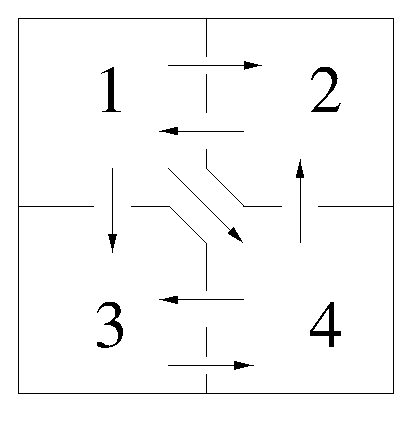
\psfig{file=figures/apart.eps,width=3.2in}}
        \caption{Schematic design of apartment passages.}
        \label{F:apart}
\end{figure}

Suppose that there is a cat in the apartment and that at each hour the cat is
asked to move from the room that it is in to another.  True to form, however,
the cat chooses with equal probability to stay in the room for another hour
or to move through one of the allowed passages.  Suppose that we let $p_{ij}$
be the probability that the cat will move from room~$i$ to room~$j$; in
particular, $p_{ii}$ is the probability that the cat will stay in room~$i$.
For example, when the cat is in room~1, it has four choices  --- it can
stay in room~1 or move to any of the other rooms.  Assuming that each of
these choices is made with equal probability, we see that
\[
p_{11} = \frac{1}{4} \qquad p_{12} = \frac{1}{4} \qquad p_{13} =
\frac{1}{4} \qquad p_{14} = \frac{1}{4}.
\]
It is now straightforward to verify that
\[
p_{21} = \frac{1}{2} \qquad p_{22} = \frac{1}{2} \qquad p_{23} = 0
\qquad p_{24} = 0
\]
\[
p_{31} = 0 \qquad p_{32} = 0 \qquad p_{33} =
\frac{1}{2} \qquad p_{34} = \frac{1}{2}
\]
\[
p_{41} = 0 \qquad p_{42} = \frac{1}{3} \qquad p_{43} =
\frac{1}{3} \qquad p_{44} = \frac{1}{3}.
\]

Putting these probabilities together yields the
{\em transition matrix}\index{matrix!transition}:
\begin{equation*} \label{E:Pexamp}
P = \left(\begin{array}{cccc}
\frac{1}{4} & \frac{1}{4} & \frac{1}{4} & \frac{1}{4} \\
\half & \half & 0 & 0 \\
 0 & 0 & \half & \half\\
0 & \frac{1}{3} & \frac{1}{3} & \frac{1}{3}
\end{array}\right)
\end{equation*}
This transition matrix has the properties that all entries are nonnegative
and that the entries in each row sum to $1$.

\subsubsection*{Three Basic Questions}

Using the transition matrix $P$, we discuss the answers to three questions:
\begin{enumerate}
\item[(A)] What is the probability that a cat starting in room~$i$ will
be in room~$j$ after exactly $k$ steps?  We call the movement that occurs
after each hour a {\em step\/}.
\item[(B)] Suppose that we put 100 cats in the apartment with some initial
distribution of cats in each room.  What will the distribution of cats
look like after a large number of steps?
\item[(C)] Suppose that a cat is initially in room~$i$ and takes a large
number of steps.  For how many of those steps will the cat be expected to
be in room~$j$?
\end{enumerate}

\subsubsection*{A Discussion of Question (A)}

We begin to answer Question (A) by determining the probability that the
cat moves from room~1 to room~4 in two steps.  We denote this probability
by $p_{14}^{(2)}$ and compute
\begin{equation} \label{E:prob14}
p_{14}^{(2)} = p_{11}p_{14} + p_{12}p_{24} + p_{13}p_{34} + p_{14}p_{44};
\end{equation}
that is, the probability is the sum of the probabilities that the cat will
move from room~$1$ to each room~$i$ and then from room~$i$ to room~4.  In
this case the answer is:
\[
p_{14}^{(2)} = \frac{1}{4}\times\frac{1}{4} + \frac{1}{4}\times0 +
\frac{1}{4}\times\frac{1}{2} + \frac{1}{4}\times\frac{1}{3} =
\frac{13}{48} \approx 0.27\;.
\]
It follows from \Ref{E:prob14} and the definition of matrix multiplication
that $p_{14}^{(2)}$ is just the $(1,4)^{th}$ entry in the matrix $P^2$.  An
induction argument shows that the probability of the cat moving from
room~$i$ to room~$j$ in $k$ steps is precisely the $(i,j)^{th}$ entry in the
matrix $P^k$ --- which answers Question (A).  In particular, we can answer the
question: What is the probability that the cat will move from room~4 to room~3
in four steps?  Using \Matlab the answer is given by typing {\tt e4\_10\_1} to
recall the matrix $P$ and then typing
\begin{verbatim}
P4 = P^4;
P4(4,3)
\end{verbatim}
obtaining
\begin{verbatim}
ans =
    0.2728
\end{verbatim}

\subsubsection*{A Discussion of Question (B)}

We answer Question (B) in two parts: first we compute a formula for
determining the number of cats that are expected to be in room~$i$ after $k$
steps, and second we explore that formula numerically for large $k$.  We
begin by supposing that 100 cats are distributed in the rooms according to
the initial vector $V_0=(v_1,v_2,v_3,v_4)^t$; that is, the number of cats
initially in room~$i$ is $v_i$.  Next, we denote the number of cats that are
expected to be in room~$i$ after $k$ steps by $v_i^{(k)}$.  For example, we
determine how many cats we expect to be in room~2 after one step.  That
number is:
\begin{equation} \label{E:probt2}
v_2^{(1)}=p_{12}v_1 + p_{22}v_2 + p_{32}v_3 + p_{42}v_4;
\end{equation}
that is, $v_2^{(1)}$ is the sum of the proportion of cats in each room~$i$
that are expected to migrate to room~2 in one step.  In this case, the answer
is:
\[
\frac{1}{4}v_1 + \frac{1}{2}v_2 + \frac{1}{3}v_4.
\]
It now follows from \Ref{E:probt2}, the definition of the transpose of a
matrix, and the definition of matrix multiplication that $v_2^{(1)}$ is
the $2^{nd}$ entry in the vector $P^tV_0$.  Indeed, it follows by induction
that $v_i^{(k)}$ is the $i^{th}$ entry in the vector $(P^t)^kV_0$ which
answers the first part of Question (B).

We may rephrase the second part of Question (B) as follows.  Let
\[
V_k = (v_1^{k},v_2^{k},v_3^{k},v_4^{k})^t = (P^t)^kV_0.
\]
Question (B) actually asks: What will the vector $V_k$ look like for
large $k$.  To answer that question we need some results about matrices
like the matrix $P$ in \Ref{E:Pexamp}.  But first we explore the answer to
this question numerically using \Matlabp.

Suppose, for example, that the initial vector is
\begin{equation*}
V_0 =\left(\begin{array}{c} 2 \\ 43 \\ 21 \\ 34 \end{array}\right).
\end{equation*}
Typing {\tt e4\_10\_1} and {\tt e4\_10\_4} enters the matrix $P$ and the
initial vector $V_0$ into \Matlabp.  To compute $V_{20}$, the distribution
of cats after $20$ steps, type
\begin{verbatim}
Q=P'
V20 = Q^(20)*V0
\end{verbatim}
and obtain
\begin{verbatim}
V20 =
   18.1818
   27.2727
   27.2727
   27.2727
\end{verbatim}
Thus, after rounding to the nearest integer, we expect $27$ cats to be in
each of rooms~2,3 and 4 and 18 cats to be in room~1 after $20$ steps.  In
fact, the vector $V_{20}$
has a remarkable feature.  Compute {\tt Q*V20} in \Matlab and see that
$V_{20} = P^tV_{20}$; that is, $V_{20}$ is, to within four digit numerical
precision, an eigenvector of $P^t$ with eigenvalue equal to $1$.  This
computation was not a numerical accident, as we now describe.  Indeed,
compute $V_{20}$ for several initial distributions $V_0$ of cats and see that
the answer will always be the same --- up to four digit accuracy.

\subsubsection*{A Discussion of Question (C)}

Suppose there is just one cat in the apartment; and we ask how many times that
cat is expected to visit room~3 in $100$ steps.  Suppose the cat starts in
room~1; then the initial distribution of cats is one cat in room~1 and zero
cats in any of the other rooms.  So $V_0=e_1$.  In our discussion of
Question (B) we saw that the $3^{rd}$ entry in $(P^t)^kV_0$ gives the
probability $c_k$ that the cat will be in room~3 after $k$ steps.

In the extreme, suppose that the probability that the cat will be in room~3 is
$1$ for each step $k$.  Then the fraction of the time that the cat is in room~3
is
\[
(1 + 1 + \cdots + 1)/100 = 1.
\]
In general, the fraction of the time $f$ that the cat will be in room~3
during a span of $100$ steps is
\[
f = \frac{1}{100}(c_1 + c_2 +\cdots + c_{100}).
\]
Since $c_k = (P^t)^kV_0$, we see that
\begin{equation}  \label{E:f}
f = \frac{1}{100}(P^tV_0 + (P^t)^2V_0 + \cdots + (P^t)^{100}V_0).
\end{equation}

So, to answer Question (C), we need a way to sum the expression for $f$
in \Ref{E:f}, at least approximately.  This is not an easy task --- though
the answer itself is easy to explain.  Let $V$ be the eigenvector of $P^t$
with eigenvalue $1$ such that the sum of the entries in $V$ is $1$.  The
answer is: $f$ is approximately equal to $V$.  See Theorem~\ref{T:ergodic}
for a more precise statement.

In our previous calculations the vector $V_{20}$ was seen to be (approximately)
an eigenvector of $P^t$ with eigenvalue $1$.  Moreover the sum of the entries
in $V_{20}$ is precisely $100$.  Therefore, we normalize $V_{20}$ to get $V$
by setting
\[
V =\frac{1}{100}V_{20}.
\]
So, the fraction of time that the cat spends in room~3 is $f\approx 0.2727$.
Indeed, we expect the cat to spend approximately $27\%$ of its time in rooms
2,3,4 and about $18\%$ of its time in room~1.

\subsection*{Markov Matrices}

We now abstract the salient properties of our cat example.  A
{\em Markov chain\/}\index{Markov chain} is a system with a
finite number of states labeled
$1$,\dots,$n$ along with probabilities $p_{ij}$ of moving from site $i$ to
site $j$ in a single step.  The Markov assumption is that these probabilities
depend only on the site that you are in and not on how you got there.  In our
example, we assumed that the probability of the cat moving from say room~2 to
room~4 did not depend on how the cat got to room~2 in the first place.

We make a second assumption: there is a $k$ such that it is possible to move
from any site $i$ to any site $j$ in exactly $k$ steps.  This assumption is
{\em not\/} valid for general Markov chains, though it is valid for the cat
example, since it is possible to move from any room to any other room in that
example in exactly three steps.  (It takes a minimum of three steps to get
from room~3 to room~1 in the cat example.)  To simplify our discussion we
include this assumption in our definition of a Markov chain.

\begin{Def}  \label{D:Markov}
{\em Markov matrices\/}\index{matrix!Markov} are square matrices
$P$ such that
\begin{enumerate}
\item[(a)]  all entries in $P$ are nonnegative,
\item[(b)]  the entries in each row of $P$ sum to $1$, and
\item[(c)]  there is a positive integer $k$ such that all of the entries
	in $P^k$ are positive.
\end{enumerate}
\end{Def}

It is straightforward to verify that parts (a) and (b) in the definition of
Markov matrices are satisfied by the transition matrix
\[
P = \left(\begin{array}{ccc} p_{11} & \cdots & p_{1n} \\
	\vdots & \vdots & \vdots \\ p_{n1} & \cdots & p_{nn}
\end{array}\right)
\]
of a Markov chain.  To verify part (c) requires further discussion.

\begin{prop}   \label{T:Markoveasy}
Let $P$ be a transition matrix\index{matrix!transition} for a
Markov chain\index{Markov chain}.
\begin{enumerate}
\item[(a)]  The probability of moving from site $i$ to site $j$ in exactly
$k$ steps is the $(i,j)^{th}$ entry in the matrix $P^k$.
\item[(b)]  The expected number of individuals at site $i$ after exactly $k$
steps is the $i^{th}$ entry in the vector $V_k\equiv (P^t)^kV_0$.
\item[(c)]  $P$ is a Markov matrix\index{matrix!Markov}.
\end{enumerate}
\end{prop}

\begin{proof} Only minor changes in our discussion of the cat example proves parts
(a) and (b) of the proposition.

(c) The assumption that it is possible to move from each site~$i$ to each
site~$j$ in exactly $k$ steps means that the $(i,j)^{th}$ entry of $P^k$ is
positive.  For that $k$, all of the entries of $P^k$ are positive.  In the
cat example, all entries of $P^3$ are positive.  \end{proof}

Proposition~\ref{T:Markoveasy} gives the answer to Question (A) and the first
part of Question (B) for general Markov chains.

Let $v_i^{(0)}\ge 0$ be the number of individuals initially at site $i$, and
let $V_0=(v_1^{(0)},\ldots,v_n^{(0)})^t$.  The total number of individuals
in the initial population is:
\[
\#(V_0) = v_1^{(0)} + \cdots + v_n^{(0)}.
\]

\begin{thm}  \label{T:Markov}
Let $P$ be a Markov matrix\index{matrix!Markov}.  Then
\begin{enumerate}
\item[(a)]  $\#(V_k)=\#(V_0)$; that is, the number of individuals after $k$
time steps is the same as the initial number.
\item[(b)]  $\dps V = \lim_{k\to\infty}V_k$ exists and $\#(V)=\#(V_0)$.
\item[(c)]  $V$ is an eigenvector of $P^t$ with eigenvalue equal to $1$.
\end{enumerate}
\end{thm}

\begin{proof}  (a) By induction it is sufficient to show that $\#(V_1)=\#(V_0)$.  We
do
this by calculating from $V_1 = P^tV_0$ that
\begin{eqnarray*}
\#(V_1) & = & v_1^{(1)} + \cdots + v_n^{(1)}\\
& = & (p_{11}v_1^{(0)} + \cdots + p_{n1}v_n^{(0)}) + \cdots +
	(p_{1n}v_1^{(0)} + \cdots + p_{nn}v_n^{(0)}) \\
& = & (p_{11}+ \cdots + p_{1n})v_1^{(0)}  + \cdots +
	(p_{n1} + \cdots + p_{nn})v_n^{(0)} \\
& = & v_1^{(0)}  + \cdots + v_n^{(0)}
\end{eqnarray*}
since the entries in each row of $P$ sum to $1$.  Thus $\#(V_1)=\#(V_0)$, as
claimed.

(b)	The hard part of this theorem is proving that the limiting vector $V$
exists; we give a proof of this fact in Chapter~\ref{C:HDeigenvalues},
Theorem~\ref{T:convergetoeig}.  Once $V$ exists it follows directly from (a)
that $\#(V)=\#(V_0)$.

(c)   	Just calculate that
\[
P^tV = P^t(\lim_{k\to\infty}V_k) = P^t(\lim_{k\to\infty}(P^t)^kV_0)
= \lim_{k\to\infty}(P^t)^{k+1}V_0 = \lim_{k\to\infty}(P^t)^kV_0 = V,
\]
which proves (c).   \end{proof}

Theorem~\ref{T:Markov}(b) gives the answer to the second part of Question (B)
for general Markov chains.  Next we discuss Question (C).

\begin{thm} \label{T:ergodic}
Let $P$ be a Markov matrix\index{matrix!Markov}.
Let $V$ be the eigenvector of $P^t$ with
eigenvalue $1$ and $\#(V)=1$.  Then after a large number of steps $N$ the
expected number of times an individual will visit site~$i$ is $Nv_i$ where
$v_i$ is the $i^{th}$ entry in $V$.
\end{thm}

\noindent {\bf Sketch of proof:}  In our discussion of Question (C) for the
cat example, we explained why the fraction $f_N$ of time that an individual
will visit site~$j$ when starting initially at site~$i$ is the $j^{th}$ entry
in the sum
\[
f_N = \frac{1}{N}(P^t + (P^t)^2 + \cdots + (P^t)^N)e_i.
\]
See \Ref{E:f}.  The proof of this theorem involves being able to calculate
the limit of $f_N$ as $N\to\infty$.  There are two main ideas.  First, the
limit of the matrix $(P^t)^N$ exists as $N$ approaches infinity --- call that
limit $Q$.  Moreover, $Q$ is a matrix all of whose columns equal $V$.
Second, for large $N$, the sum
\[
P^t + (P^t)^2 + \cdots + (P^t)^N \approx Q + Q + \cdots + Q = NQ,
\]
so that the limit of the $f_N$ is $Qe_i=V$.

The verification of these statements is beyond the scope of this text.
For those interested, the idea of the proof of the second part is roughly the
following.  Fix $k$ large enough so that $(P^t)^k$ is close to $Q$.  Then when
$N$ is large, much larger than $k$, the sum of the first $k$ terms in the
series is nearly zero.  \end{proof}


Theorem~\ref{T:ergodic} gives the answer to Question (C) for a general Markov
chain.  It follows from Theorem~\ref{T:ergodic} that for Markov chains the
amount of time that an individual spends in room~$i$ is independent of the
individual's initial room --- at least after a large number of steps.

A complete proof of this theorem relies on a result known as the {\em ergodic
theorem}.
Roughly speaking, the ergodic theorem relates space averages
with time averages.   To see how this point is relevant, note that Question (B)
deals with the issue of how a large number of individuals will be distributed
in space after a large number of steps, while Question (C) deals with the
issue of how the path of a single individual will be distributed in time after
a large number of steps.

\subsubsection*{An Example of Umbrellas}

This example focuses on the utility of answering Question (C) and reinforces
the fact that results in Theorem~\ref{T:Markov} have the second
interpretation given in Theorem~\ref{T:ergodic}.

Consider the problem of a man with four umbrellas.  If it is raining in the
morning when the man is about to leave for his office, then the man takes an
umbrella from home to office, assuming that he has an umbrella at home.  If it
is raining in the afternoon, then the man takes an umbrella from office to
home, assuming that he has an umbrella in his office.  Suppose that the
probability that it will rain in the morning is $p=0.2$ and the probability
that it will rain in the afternoon is $q=0.3$, and these probabilities are
independent.  What percentage of days will the man get wet going from home
to office; that is, what percentage of the days will the man be at home on a
rainy morning with all of his umbrellas at the office?

There are five states in the system depending on the number of umbrellas that
are at home.  Let $s_i$ where $0\leq i\leq 4$ be the state with $i$ umbrellas
at home and $4-i$ umbrellas at work.  For example, $s_2$ is the state of
having two umbrellas at home and two at the office.  Let $P$ be the
$5\times 5$ transition matrix of state changes from morning to afternoon and
$Q$ be the $5\times 5$ transition matrix of state changes from afternoon to
morning.  For example, the probability $p_{23}$ of moving from site $s_2$ to
site $s_3$ is $0$, since it is not possible to have more umbrellas at home
after going to work in the morning.  The probability $q_{23}=q$, since the
number of umbrellas at home will increase by one only if it is raining in the
afternoon.  The transition probabilities between all states are given in the
following transition matrices:
\[
P = \left(\begin{array}{ccccc} 1 & 0 & 0 & 0 & 0 \\
  p & 1-p & 0 & 0 & 0 \\ 0 & p & 1-p & 0 & 0 \\ 0 & 0 & p & 1-p & 0 \\
 0 & 0 & 0 & p & 1-p \end{array}\right); \quad
Q = \left(\begin{array}{ccccc} 1-q & q & 0 & 0 & 0 \\
  0 & 1-q & q & 0 & 0 \\ 0 & 0 & 1-q & q & 0 \\ 0 & 0 & 0 & 1-q & q \\
 0 & 0 & 0 & 0 & 1 \end{array}\right)
\]
Specifically,
\begin{equation*}
P =
\left(\begin{array}{ccccc} 1 & 0 & 0 & 0 & 0 \\
  0.2 & 0.8 & 0 & 0 & 0 \\ 0 & 0.2 & 0.8 & 0 & 0 \\ 0 & 0 & 0.2 & 0.8 & 0 \\
 0 & 0 & 0 & 0.2 & 0.8 \end{array}\right) \AND
Q =
\left(\begin{array}{ccccc} 0.7 & 0.3 & 0 & 0 & 0 \\
  0 & 0.7 & 0.3 & 0 & 0 \\ 0 & 0 & 0.7 & 0.3 & 0 \\ 0 & 0 & 0 & 0.7 & 0.3 \\
 0 & 0 & 0 & 0 & 1 \end{array}\right)
\end{equation*}

The transition matrix\index{matrix!transition} $M$ from
moving from state $s_i$ on one morning to
state $s_j$ the next morning is just $M=PQ$.  We can compute this matrix
using \Matlab by typing
\begin{verbatim}
e4_10_6
M = P*Q
\end{verbatim}
obtaining
\begin{verbatim}
M =
    0.7000    0.3000         0         0         0
    0.1400    0.6200    0.2400         0         0
         0    0.1400    0.6200    0.2400         0
         0         0    0.1400    0.6200    0.2400
         0         0         0    0.1400    0.8600
\end{verbatim}
It is easy to check using \Matlab that all entries in the matrix $M^4$ are
nonzero.  So $M$ is a Markov matrix\index{matrix!Markov} and we can use
Theorem~\ref{T:ergodic}
to find the limiting distribution of states.  Start with some initial
condition like $V_0=(0,0,1,0,0)^t$ corresponding to the state in which two
umbrellas are at home and two at the office.  Then compute the vectors
$V_k=(M^t)^kV_0$ until arriving at an eigenvector of $M^t$ with eigenvalue 1.
For example, $V_{70}$ is computed by typing \verb+V70 = M'^(70)*V0+ and
obtaining
\begin{verbatim}
V70 =
    0.0419
    0.0898
    0.1537
    0.2633
    0.4512
\end{verbatim}
We interpret $V\approx V_{70}$ in the following way.  Since $v_1$ is
approximately $.042$, it follows that for approximately $4.2\%$ of all steps 
the umbrellas are in state $s_0$.  That is, approximately $4.2\%$ of all days 
there are no umbrellas at home.  The probability that it will rain in the 
morning on one of those days is $0.2$.  Therefore, the probability of being 
at home in the morning when it is raining without any umbrellas is 
approximately $0.008$.





\EXER

\TEXER

\begin{exercise} \label{c4.10.1}
Let $P$ be a Markov matrix and let $w=(1,\ldots,1)^t$.  Show that
the vector $w$ is an eigenvector of $P$ with eigenvalue $1$.
\end{exercise}

\noindent In Exercises~\ref{c4.10.2a} -- \ref{c4.10.2c} which of the
matrices are Markov matrices, and why?
\begin{exercise} \label{c4.10.2a}
$P = \mattwo{0.8}{0.2}{0.2}{0.8}$.
\end{exercise}
\begin{exercise} \label{c4.10.2b}
$Q = \mattwo{0.8}{0.2}{0}{1}$.
\end{exercise}
\begin{exercise} \label{c4.10.2c}
$R = \mattwo{0.8}{0.2}{-0.2}{1.2}$.
\end{exercise}

\begin{exercise} \label{c4.10.3}
The state diagram of a Markov chain is given in Figure~\ref{F:Mchain}.
Assume that each arrow leaving a state has equal probability of being chosen.
Find the transition matrix for this chain.
\end{exercise}
\begin{figure}[htb]
        \centerline{%
        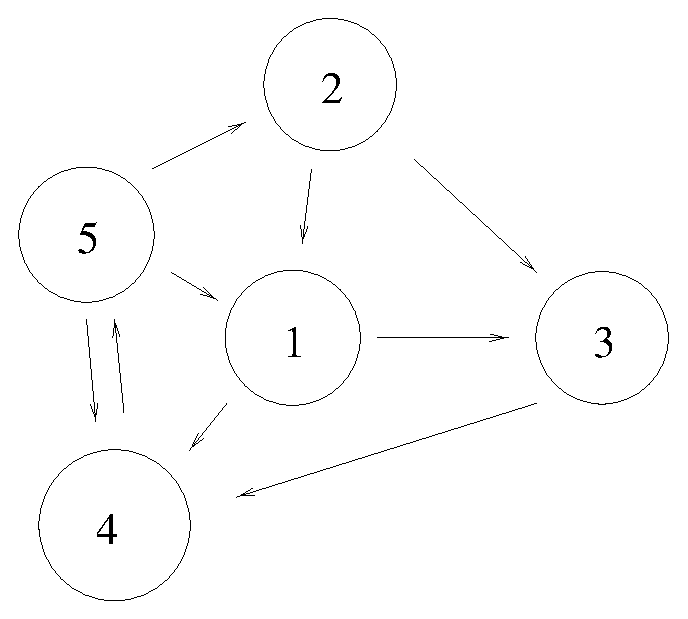
\psfig{file=figures/Mchain.eps,width=3.0in}}
        \caption{State diagram of a Markov chain.}
        \label{F:Mchain}
\end{figure}


\begin{exercise} \label{c4.10.4}
Suppose that $P$ and $Q$ are each $n\times n$ matrices whose rows sum to $1$.
Show that $PQ$ is also an $n\times n$ matrix whose rows sum to $1$.
\end{exercise}



\CEXER

\begin{exercise} \label{c4.10.5}
Suppose the apartment in Figure~\ref{F:apart} is populated by dogs rather than
cats.  Suppose that dogs will actually move when told; that is, at each step
a dog will move from the room that he occupies to another room.
\begin{itemize}
\item[(a)]  Calculate the transition matrix {\tt PDOG} for this Markov chain
and verify that {\tt PDOG} is a Markov matrix.
\item[(b)]  Find the probability that a dog starting in room~2 will end up in
room~3 after $5$ steps.
\item[(c)]  Find the probability that a dog starting in room~3 will end up in
room~1 after $4$ steps.  Explain why your answer is correct without using
\Matlabp.
\item[(d)]  Suppose that the initial population consists of 100 dogs.  After
a large number of steps what will be the distribution of the dogs in the four
rooms.
\end{itemize}
\end{exercise}

\begin{exercise} \label{c4.10.6}
A truck rental company has locations in three cities A, B and C.
Statistically, the company knows that the trucks rented at one location will
be returned in one week to the three locations in the following proportions.
\begin{center}
\begin{tabular}{|c||c|c|c|}
\hline
Rental Location &  Returned to A & Returned to B & Returned to C\\
\hline
A  & 75\% & 10\%  & 15\% \\
\hline
B & 5\% & 85\% & 10\% \\
\hline
C & 20\% & 20\% & 60\%\\
\hline
\end{tabular}
\end{center}
Suppose that the company has 250 trucks.  How should the company distribute
the trucks so that the number of trucks available at each location remains
approximately constant from one week to the next?
\end{exercise}

\begin{exercise} \label{c4.10.7}
Let
\begin{equation*}
P = \left(\begin{array}{ccccc}
 0.10 & 0.20 & 0.30 & 0.15 & 0.25\\
 0.05 & 0.35 & 0.10 & 0.40 & 0.10\\
   0  &   0  & 0.35 & 0.55 & 0.10\\
 0.25 & 0.25 & 0.25 & 0.25 &   0\\
 0.33 & 0.32 &   0  &   0  & 0.35
\end{array}\right)
\end{equation*}
be the transition matrix of a Markov chain.
\begin{itemize}
\item[(a)]  What is the probability that an individual at site~2 will move to
site~5 in three steps?
\item[(b)]  What is the probability that an individual at site~4 will move to
site~1 in seven steps?
\item[(c)]  Suppose that 100 individuals are initially uniformly distributed
at the five sites.  How will the individuals be distributed after four steps?
\item[(d)]  Find an eigenvector of $P^t$ with eigenvalue $1$.
\end{itemize}
\end{exercise}

\begin{exercise} \label{c4.10.8}
Suppose that the probability that it will rain in the morning in $p=0.3$ and
the probability that it will rain in the afternoon is $q=0.25$.  In the man
with umbrellas example, what is the probability that the man will be at home
with no umbrellas while it is raining?
\end{exercise}

\begin{exercise} \label{c4.10.9}
Suppose that the original man in the text with umbrellas has only three
umbrellas instead of four.  What is the probability that on a given day he
will get wet going to work?
\end{exercise}



\end{document}

\documentclass{ximera}

 

\usepackage{epsfig}

\graphicspath{
  {./}
  {figures/}
}

\usepackage{morewrites}
\makeatletter
\newcommand\subfile[1]{%
\renewcommand{\input}[1]{}%
\begingroup\skip@preamble\otherinput{#1}\endgroup\par\vspace{\topsep}
\let\input\otherinput}
\makeatother

\newcommand{\includeexercises}{\directlua{dofile("/home/jim/linearAlgebra/laode/exercises.lua")}}

%\newcounter{ccounter}
%\setcounter{ccounter}{1}
%\newcommand{\Chapter}[1]{\setcounter{chapter}{\arabic{ccounter}}\chapter{#1}\addtocounter{ccounter}{1}}

%\newcommand{\section}[1]{\section{#1}\setcounter{thm}{0}\setcounter{equation}{0}}

%\renewcommand{\theequation}{\arabic{chapter}.\arabic{section}.\arabic{equation}}
%\renewcommand{\thefigure}{\arabic{chapter}.\arabic{figure}}
%\renewcommand{\thetable}{\arabic{chapter}.\arabic{table}}

%\newcommand{\Sec}[2]{\section{#1}\markright{\arabic{ccounter}.\arabic{section}.#2}\setcounter{equation}{0}\setcounter{thm}{0}\setcounter{figure}{0}}

\newcommand{\Sec}[2]{\section{#1}}

\setcounter{secnumdepth}{2}
%\setcounter{secnumdepth}{1} 

%\newcounter{THM}
%\renewcommand{\theTHM}{\arabic{chapter}.\arabic{section}}

\newcommand{\trademark}{{R\!\!\!\!\!\bigcirc}}
%\newtheorem{exercise}{}

\newcommand{\dfield}{{\sf dfield9}}
\newcommand{\pplane}{{\sf pplane9}}

\newcommand{\EXER}{\section*{Exercises}}%\vspace*{0.2in}\hrule\small\setcounter{exercise}{0}}
\newcommand{\CEXER}{}%\vspace{0.08in}\begin{center}Computer Exercises\end{center}}
\newcommand{\TEXER}{} %\vspace{0.08in}\begin{center}Hand Exercises\end{center}}
\newcommand{\AEXER}{} %\vspace{0.08in}\begin{center}Hand Exercises\end{center}}

% BADBAD: \newcommand{\Bbb}{\bf}

\newcommand{\R}{\mbox{$\Bbb{R}$}}
\newcommand{\C}{\mbox{$\Bbb{C}$}}
\newcommand{\Z}{\mbox{$\Bbb{Z}$}}
\newcommand{\N}{\mbox{$\Bbb{N}$}}
\newcommand{\D}{\mbox{{\bf D}}}
\usepackage{amssymb}
%\newcommand{\qed}{\hfill\mbox{\raggedright$\square$} \vspace{1ex}}
%\newcommand{\proof}{\noindent {\bf Proof:} \hspace{0.1in}}

\newcommand{\setmin}{\;\mbox{--}\;}
\newcommand{\Matlab}{{M\small{AT\-LAB}} }
\newcommand{\Matlabp}{{M\small{AT\-LAB}}}
\newcommand{\computer}{\Matlab Instructions}
\newcommand{\half}{\mbox{$\frac{1}{2}$}}
\newcommand{\compose}{\raisebox{.15ex}{\mbox{{\scriptsize$\circ$}}}}
\newcommand{\AND}{\quad\mbox{and}\quad}
\newcommand{\vect}[2]{\left(\begin{array}{c} #1_1 \\ \vdots \\
 #1_{#2}\end{array}\right)}
\newcommand{\mattwo}[4]{\left(\begin{array}{rr} #1 & #2\\ #3
&#4\end{array}\right)}
\newcommand{\mattwoc}[4]{\left(\begin{array}{cc} #1 & #2\\ #3
&#4\end{array}\right)}
\newcommand{\vectwo}[2]{\left(\begin{array}{r} #1 \\ #2\end{array}\right)}
\newcommand{\vectwoc}[2]{\left(\begin{array}{c} #1 \\ #2\end{array}\right)}

\newcommand{\ignore}[1]{}


\newcommand{\inv}{^{-1}}
\newcommand{\CC}{{\cal C}}
\newcommand{\CCone}{\CC^1}
\newcommand{\Span}{{\rm span}}
\newcommand{\rank}{{\rm rank}}
\newcommand{\trace}{{\rm tr}}
\newcommand{\RE}{{\rm Re}}
\newcommand{\IM}{{\rm Im}}
\newcommand{\nulls}{{\rm null\;space}}

\newcommand{\dps}{\displaystyle}
\newcommand{\arraystart}{\renewcommand{\arraystretch}{1.8}}
\newcommand{\arrayfinish}{\renewcommand{\arraystretch}{1.2}}
\newcommand{\Start}[1]{\vspace{0.08in}\noindent {\bf Section~\ref{#1}}}
\newcommand{\exer}[1]{\noindent {\bf \ref{#1}}}
\newcommand{\ans}{}
\newcommand{\matthree}[9]{\left(\begin{array}{rrr} #1 & #2 & #3 \\ #4 & #5 & #6
\\ #7 & #8 & #9\end{array}\right)}
\newcommand{\cvectwo}[2]{\left(\begin{array}{c} #1 \\ #2\end{array}\right)}
\newcommand{\cmatthree}[9]{\left(\begin{array}{ccc} #1 & #2 & #3 \\ #4 & #5 &
#6 \\ #7 & #8 & #9\end{array}\right)}
\newcommand{\vecthree}[3]{\left(\begin{array}{r} #1 \\ #2 \\
#3\end{array}\right)}
\newcommand{\cvecthree}[3]{\left(\begin{array}{c} #1 \\ #2 \\
#3\end{array}\right)}
\newcommand{\cmattwo}[4]{\left(\begin{array}{cc} #1 & #2\\ #3
&#4\end{array}\right)}

\newcommand{\Matrix}[1]{\ensuremath{\left(\begin{array}{rrrrrrrrrrrrrrrrrr} #1 \end{array}\right)}}

\newcommand{\Matrixc}[1]{\ensuremath{\left(\begin{array}{cccccccccccc} #1 \end{array}\right)}}



\renewcommand{\labelenumi}{\theenumi)}
\newenvironment{enumeratea}%
{\begingroup
 \renewcommand{\theenumi}{\alph{enumi}}
 \renewcommand{\labelenumi}{(\theenumi)}
 \begin{enumerate}}
 {\end{enumerate}\endgroup}



\newcounter{help}
\renewcommand{\thehelp}{\thesection.\arabic{equation}}

%\newenvironment{equation*}%
%{\renewcommand\endequation{\eqno (\theequation)* $$}%
%   \begin{equation}}%
%   {\end{equation}\renewcommand\endequation{\eqno \@eqnnum
%$$\global\@ignoretrue}}

%\input{psfig.tex}

\author{Martin Golubitsky and Michael Dellnitz}

%\newenvironment{matlabEquation}%
%{\renewcommand\endequation{\eqno (\theequation*) $$}%
%   \begin{equation}}%
%   {\end{equation}\renewcommand\endequation{\eqno \@eqnnum
% $$\global\@ignoretrue}}

\newcommand{\soln}{\textbf{Solution:} }
\newcommand{\exercap}[1]{\centerline{Figure~\ref{#1}}}
\newcommand{\exercaptwo}[1]{\centerline{Figure~\ref{#1}a\hspace{2.1in}
Figure~\ref{#1}b}}
\newcommand{\exercapthree}[1]{\centerline{Figure~\ref{#1}a\hspace{1.2in}
Figure~\ref{#1}b\hspace{1.2in}Figure~\ref{#1}c}}
\newcommand{\para}{\hspace{0.4in}}

\renewenvironment{solution}{\suppress}{\endsuppress}

\ifxake
\newenvironment{matlabEquation}{\begin{equation}}{\end{equation}}
\else
\newenvironment{matlabEquation}%
{\let\oldtheequation\theequation\renewcommand{\theequation}{\oldtheequation*}\begin{equation}}%
  {\end{equation}\let\theequation\oldtheequation}
\fi

\makeatother


\title{c5.tex}

\begin{document}
\begin{abstract}
BADBAD
\end{abstract}
\maketitle

\chapter{Vector Spaces}
\label{C:vectorspaces}

\normalsize

In Chapter~\ref{lineq} we discussed how to solve systems of $m$
linear equations in $n$ unknowns.  We found that solutions of
these equations are vectors $(x_1,\ldots,x_n)\in\R^n$.  
In Chapter~\ref{chap:matrices} we discussed how the notation of
matrices and matrix multiplication drastically simplifies the
presentation of linear systems and how matrix multiplication
leads to linear mappings.  We also discussed briefly how linear
mappings lead to methods for solving linear systems ---
superposition, eigenvectors, inverses.  In
Chapter~\ref{chap:SolveOdes} we discussed how to solve systems
of $n$ linear differential equations in $n$ unknown functions.
These chapters have
provided an introduction to many of the ideas of linear algebra
and now we begin the task of formalizing these ideas.

Sets having the two operations of vector addition and scalar
multiplication are called {\em vector spaces\/}.  This concept
is introduced in Section~\ref{S:5.1} along with the two
primary examples --- the set $\R^n$ in which solutions to systems
of linear equations sit and the set $\CCone$ of differentiable
functions in which solutions to systems of ordinary differential
equations sit.  Solutions to systems of homogeneous linear equations
form subspaces of $\R^n$ and solutions of systems of linear
differential equations form subspaces of $\CCone$.  These issues
are discussed in Sections~\ref{S:5.1} and \ref{S:5.2}.

When we {\em solve\/} a homogeneous system of equations, we write
every solution as a superposition of a finite number of specific
solutions.  Abstracting this process is one of the main points of this
chapter.  Specifically, we show that every vector in many commonly
occurring vector spaces
(in particular, the subspaces of solutions) can be written as a
{\em linear combination\/} (superposition) of a few 
solutions.  The minimum number of solutions needed is called
the {\em dimension\/} of that vector space.  Sets of vectors that 
generate all solutions by superposition and that consist of that minimum 
number of vectors are called {\em bases\/}.  These ideas are discussed
in detail in Sections~\ref{S:5.3}--\ref{S:5.5}.  The proof of
the main theorem (Theorem~\ref{basis=span+indep}), which gives a
computable method for determining when a set is a basis, is given in
Section~\ref{S:5.6}.  This proof may be omitted on a first reading,
but the statement of the theorem is most important and must be
understood.


\section{Vector Spaces and Subspaces} \label{S:5.1}

Vector spaces abstract the arithmetic properties of addition and
scalar multiplication of vectors.  In $\R^n$ we know how to add
vectors and to multiply vectors by scalars.  Indeed, it is
straightforward to verify that each of the eight
properties listed in Table~\ref{vectorspacelist} is valid for
vectors in $V=\R^n$.  Remarkably, sets that satisfy these eight
properties have much in common with $\R^n$.  So we define:
\begin{Def}  \label{vectorspace}
Let $V$ be a set having the two operations of addition and scalar
multiplication.  Then $V$ is a {\em vector space\/} if the eight
properties listed in Table~\ref{vectorspace} hold.  The elements
of a vector space are called {\em vectors}\index{vector}.
\end{Def} \index{vector!space}\index{vector!space}

The vector $0$ mentioned in (A3) in Table~\ref{vectorspacelist}
is called the {\em zero vector}\index{zero vector}.

\begin{table}
\caption{Properties of Vector Spaces: suppose $u,v,w\in V$ and
$r,s\in\R$.}
\begin{center}
\begin{tabular}{|c|c|c|}
\hline
(A1) & Addition is commutative & $v+w=w+v$ \\
\hline
(A2) & Addition is associative & $(u+v)+w = u+(v+w)$ \\
\hline
(A3) & Additive identity $0$ exists & $v+0=v$ \\
\hline
(A4) & Additive inverse $-v$ exists & $v+(-v) = 0$ \\
\hline
(M1) & Multiplication is associative & $(rs)v = r(sv)$ \\
\hline
(M2) & Multiplicative identity exists & $1v=v$ \\
\hline
(D1) & Distributive law for scalars & $(r+s)v = rv+sv$ \\
\hline
(D2) & Distributive law for vectors & $r(v+w) = rv+rw$ \\
\hline
\end{tabular}
\end{center} \index{scalar multiplication} \index{vector!addition}
\index{associative} \index{distributive}
\index{commutative} \index{inverse}
\label{vectorspacelist}
\end{table}

When we say that a vector space $V$ has the two operations of
addition and scalar multiplication we mean that the sum of two
vectors in $V$ is again a vector in $V$ and the scalar product
of a vector with a number is again a vector in $V$.  These two
properties are called {\em closure under addition\/} and
{\em closure under scalar multiplication}.
\index{closure!under addition}
\index{closure!under scalar multiplication}

In this discussion we focus on just two types of vector spaces:
$\R^n$ and function spaces.  The reason that we make this choice
is that solutions to linear equations are vectors in $\R^n$ while
solutions to linear systems of differential equations are vectors
of functions.

\subsubsection*{An Example of a Function Space}
\index{function space}

For example, let ${\cal F}$ denote the set of all functions $f:\R\to\R$.
Note that functions like $f_1(t)=t^2-2t+7$ and $f_2(t)=\sin t$ are in
${\cal F}$ since they are defined for all real numbers $t$, but that functions
like $g_1(t)=\frac{1}{t}$ and $g_2(t)=\tan t$ are not in ${\cal F}$ since
they are not defined for all $t$.

We can add two functions $f$ and $g$ by defining the function $f+g$ to be:
\[
(f+g)(t) = f(t) + g(t).
\]
We can also multiply a function $f$ by a scalar $c\in\R$ by defining the
function $cf$ to be:
\[
(cf)(t) = cf(t).
\]
With these operations of addition and scalar multiplication, ${\cal F}$
is a vector space; that is, ${\cal F}$ satisfies the eight vector space
properties in Table~\ref{vectorspacelist}.  More precisely:
\begin{itemize}
\item[(A3)] Define the zero function ${\cal O}$ by
\[
     {\cal O}(t) = 0 \quad \mbox{for all $t\in\R$.}
\]
For every $x$ in ${\cal F}$ the function ${\cal O}$ satisfies:
\[
     (x+{\cal O})(t) = x(t) + {\cal O}(t) = x(t) + 0 = x(t).
\]
Therefore, $x+{\cal O}=x$ and ${\cal O}$ is the additive
identity in ${\cal F}$.
\item[(A4)] Let $x$ be a function in ${\cal F}$ and define $y(t)=-x(t)$.
Then $y$ is also a function in ${\cal F}$, and
\[
    (x+y)(t) =  x(t) + y(t) = x(t) + (-x(t)) = 0 = {\cal O}(t).
\]
Thus, $x$ has the additive inverse $-x$.
\end{itemize}
After these comments it is straightforward to verify that the
remaining six properties in Table~\ref{vectorspacelist} are
satisfied by functions in ${\cal F}$.

\subsubsection*{Sets that are not Vector Spaces}
\index{vector!space}\index{vector!space}

It is worth considering how closure under vector addition and
scalar multiplication can fail.  Consider the following three
examples.

\begin{enumerate}
\item[(i)] Let $V_1$ be the set that consists of just the $x$
and $y$ axes in the plane.  Since $(1,0)$ and $(0,1)$ are in
$V_1$ but
\[
(1,0) + (0,1) = (1,1)
\]
is not in $V_1$, we see that $V_1$ is not closed under vector
addition. On the other hand, $V_1$ is closed under scalar
multiplication.  \index{closure!under addition}
\index{closure!under scalar multiplication}


\item[(ii)] Let $V_2$ be the set of all vectors $(k,\ell)\in\R^2$
where $k$ and $\ell$ are integers.  The set $V_2$ is closed under
addition but not under scalar multiplication since
$\half(1,0)=(\half,0)$ is not in $V_2$.

\item[(iii)] Let $V_3=[1,2]$ be the closed interval in $\R$. The
set $V_3$ is neither closed under addition ($1+1.5=2.5\not\in
V_3$) nor under scalar multiplication ($4\cdot 1.5 = 6\not\in
V_3$).  Hence the set $V_3$ is not closed under vector addition
and not closed under scalar multiplication.
\end{enumerate}

\subsection*{Subspaces}

\begin{Def} \label{subspaces}
Let $V$ be a vector space.  A nonempty subset $W\subset V$ is a
{\em subspace\/} if $W$ is a vector space using the operations of 
addition and scalar multiplication defined on $V$.
\end{Def} \index{subspace}

Note that in order for a subset $W$ of a vector space $V$ to be a 
subspace it must be {\em closed under addition\/} and {\em closed under
scalar multiplication\/}.  That is, suppose $w_1,w_2\in W$ and 
$r\in\R$.  Then
\begin{itemize}
\item[(i)]  $w_1+w_2 \in W$, and
\item[(ii)]  $rw_1\in W$.
\end{itemize}
\index{vector!addition} \index{scalar multiplication}

The $x$-axis and the $xz$-plane are examples of subsets of $\R^3$
that are closed under addition and closed under scalar multiplication.
Every vector on the $x$-axis has the form $(a,0,0)\in\R^3$.
The sum of two vectors $(a,0,0)$ and $(b,0,0)$ on the $x$-axis is
$(a+b,0,0)$ which is also on the $x$-axis.  The $x$-axis
is also closed under scalar multiplication as $r(a,0,0)=(ra,0,0)$,
and the $x$-axis is a subspace of $\R^3$.  Similarly, every vector
in the $xz$-plane in $\R^3$ has the form $(a_1,0,a_3)$. As in the
case of the $x$-axis, it is easy to verify that this set of vectors
is closed under addition and scalar multiplication.  Thus, the
$xz$-plane is also a subspace of $\R^3$.

In Theorem~\ref{T:subspaces} we show that every subset of a vector space 
that is closed under addition and scalar multiplication is a subspace.  
To verify this statement, we need the following lemma in which some special 
notation is used.  Typically, we use the same notation $0$ to denote the
real number zero and the zero vector\index{zero vector}.  In the following
lemma it is convenient to distinguish the two different uses of $0$, and we 
write the zero vector in boldface.

\begin{lemma}  \label{lem:AddId}
Let $V$ be a vector space, and let ${\bf 0}\in V$ be the zero vector.  Then
\[
0v={\bf 0} \quad \mbox{and}\quad (-1)v=-v
\]
for every vector in $v\in V$.
\end{lemma}

\begin{proof} Let $v$ be a vector in $V$ and use (D1) to compute
\[
     0v + 0v  = (0+0)v = 0v.
\]
By (A4) the vector $0v$ has an additive inverse $-0v$.  Adding $-0v$ 
to both sides yields 
\[
(0v + 0v) + (-0v) = 0v + (-0v) = {\bf 0}.
\] 
Associativity of addition (A2) now implies 
\[
0v + (0v + (-0v)) = {\bf 0}.
\]
A second application of (A4) implies that 
\[
0v + {\bf 0} = {\bf 0}
\]
and (A3) implies that $0v={\bf 0}$.

Next, we show that the additive inverse $-v$ of a vector $v$ is unique. 
That is, if $v + a = {\bf 0}$, then $a=-v$.  

Before beginning the proof, note that commutativity of addition (A1) together 
with (A3) implies that ${\bf 0}+v=v$.  Similarly, (A1) and (A4) imply that 
$-v+v={\bf 0}$.  

To prove uniqueness of additive inverses, add $-v$ to both sides of the 
equation $v + a = {\bf 0}$ yielding 
\[
-v + (v + a) = -v + {\bf 0}. 
\]
Properties (A2) and (A3) imply
\[
(-v + v) + a = -v.
\]
But 
\[
(-v + v) + a = {\bf 0} + a = a.
\]
Therefore $a = -v$, as claimed.

To verify that $(-1)v = -v$, we show that $(-1)v$ is the
additive inverse of $v$.  Using (M1), (D1), and the fact that $0v = {\bf 0}$, 
calculate
\[
     v + (-1)v = 1v + (-1)v =(1-1)v = 0v = {\bf 0}.
\]
Thus, $(-1)v$ is the additive inverse of $v$ and must equal $-v$, as
claimed.  \end{proof}

\begin{thm}  \label{T:subspaces}
Let $W$ be a subset of the vector space $V$. If $W$ is closed under addition 
and closed under scalar multiplication, then $W$ is a subspace.
\end{thm}\index{subspace}
\begin{proof}  We have to show that $W$ is a vector space using the operations 
of addition and scalar multiplication defined on $V$.  That is, we need to
verify that the eight properties listed in Table~\ref{vectorspacelist} are 
satisfied.  Note that properties (A1), (A2), (M1), (M2), (D1), and (D2) are 
valid for vectors in $W$ since they are valid for vectors in $V$.

It remains to verify (A3) and (A4).  Let $w\in W$ be any vector.
Since $W$ is closed under scalar multiplication, it follows that
$0w$ and $(-1)w$ are in $W$. Lemma~\ref{lem:AddId} states that
$0w=0$ and $(-1)w=-w$; it follows that $0$ and $-w$ are in $W$.
Hence, properties (A3) and (A4) are valid for vectors in $W$,
since they are valid for vectors in $V$.  \end{proof}

\subsubsection*{Examples of Subspaces of $\R^n$}

\begin{exam}  \label{EX:subspaces}
{\rm
\begin{itemize}
\item[(a)] Let $V$ be a vector space.  Then the subsets $V$ and $\{0\}$ are
always subspaces of $V$.  A subspace $W\subset V$ is {\em proper\/} if
$W\neq 0$ and $W\neq V$. \index{subspace!proper}
\item[(b)] Lines through the origin are subspaces of $\R^n$.  Let $w\in \R^n$
be a nonzero vector and let $W=\{rw:r\in\R\}$.  The set $W$ is closed under
addition and scalar multiplication and is a subspace of $\R^n$ by 
Theorem~\ref{T:subspaces}.
The subspace $W$ is just a {\em line through the origin\/} in $\R^n$, since
the vector $rw$ points in the same direction as $w$ when $r>0$ and the exact
opposite direction when $r<0$.
\item[(c)]  Planes containing the origin are subspaces of $\R^3$.  To verify
this point, let $P$ be a plane through the origin and let $N$ be a vector
perpendicular\index{perpendicular} to $P$.  Then $P$ consists of all vectors
$v\in\R^3$ perpendicular to $N$; using the dot-product (see Chapter~\ref{lineq},
\Ref{XX_0}) we recall that such vectors satisfy the linear equation
$N\cdot v = 0$.  By superposition\index{superposition}, the set of all
solutions to this equation is closed under addition and scalar multiplication
and is therefore a subspace by Theorem~\ref{T:subspaces}.
\end{itemize}
}
\end{exam}
In a sense that will be made precise all subspaces of $\R^n$ can be written
as the span of a finite number of vectors generalizing
Example~\ref{EX:subspaces}(b) or as solutions to a system of linear equations
generalizing Example~\ref{EX:subspaces}(c).


\subsubsection*{Examples of Subspaces of the Function Space ${\cal F}$}
\index{function space!subspace of}\index{subspace!of function space}

Let ${\cal P}$ be the set of all polynomials in ${\cal F}$.  The sum of
two polynomials is a polynomial and the scalar multiple of a polynomial is a
polynomial.  Thus, ${\cal P}$ is closed under addition and scalar
multiplication, and ${\cal P}$ is a subspace of ${\cal F}$.

As a second example of a subspace of ${\cal F}$, let $\CCone$ be the set of
all continuously differentiable functions $u:\R\to\R$.  A function $u$ is
in $\CCone$ if $u$ and $u'$ exist and are continuous for all $t\in\R$.
Examples of functions in $\CCone$ are:
\begin{enumerate}
\item[(i)] Every polynomial $p(t)=a_mt^m+a_{m-1}t^{m-1}+\cdots
+a_1t+a_0$ is in $\CCone$. \index{polynomial}
\item[(ii)]  The function $u(t)=e^{\lambda t}$ is in $\CCone$
for each constant $\lambda\in\R$.
\item[(iii)]  The trigonometric functions $u(t)=\sin(\lambda t)$
and $v(t)=\cos(\lambda t)$ are in $\CCone$ for each constant
$\lambda\in\R$. \index{trigonometric function}
\item[(iv)] $u(t)=t^{7/3}$ is twice differentiable everywhere and is
in $\CCone$.
\end{enumerate}
Equally there are many commonly used functions that are not in
$\CCone$.  Examples include:
\begin{enumerate}
\item[(i)] $u(t)=\frac{1}{t-5}$ is neither defined nor
continuous at $t=5$.
\item[(ii)] $u(t)=|t|$ is not differentiable (at $t=0$).
\item[(iii)] $u(t)=\csc(t)$ is neither defined nor continuous at
$t=k\pi$ for any integer $k$.
\end{enumerate}

The subset $\CCone\subset{\cal F}$  is a subspace and hence a vector space.
\index{vector!in $\CCone$}
The reason is simple.  If $x(t)$ and $y(t)$ are continuously differentiable,
then
\[
\frac{d}{dt}(x+y) = \frac{dx}{dt}+\frac{dy}{dt}.
\]
Hence $x+y$ is differentiable and is in $\CCone$ and $\CCone$ is closed under
addition.  Similarly, $\CCone$ is closed under scalar multiplication.  Let
$r\in\R$ and let $x\in\CCone$. Then
\[
\frac{d}{dt}(rx)(t) = r\frac{dx}{dt}(t).
\]
Hence $rx$ is differentiable and is in $\CCone$.

\subsubsection*{The Vector Space $(\CCone)^n$}

Another example of a vector space that combines the features of
both $\R^n$ and $\CCone$ is $(\CCone)^n$.  Vectors
$u\in (\CCone)^n$ have the form
\[
u(t) = (u_1(t),\ldots,u_n(t)),
\]
where each coordinate function $u_j(t)\in\CCone$.  Addition and
scalar multiplication in $(\CCone)^n$ are defined coordinatewise
--- just like addition and scalar multiplication in $\R^n$.
That is, let $u,v$ be in $(\CCone)^n$ and let $r$ be in $\R$, then
\begin{eqnarray*}
(u+v)(t) & = & (u_1(t)+v_1(t),\ldots,u_n(t)+v_n(t)) \\
(ru)(t) & = & (ru_1(t),\ldots,ru_n(t)).
\end{eqnarray*}
The set $(\CCone)^n$ satisfies the eight properties of vector spaces and
is a vector space.  Solutions to systems of $n$ linear ordinary differential
equations are vectors in $(\CCone)^n$.


\EXER

\TEXER

\begin{exercise} \label{c5.1.1}
Verify that the set $V_1$ consisting of all scalar multiples of
$(1,-1,-2)$ is a subspace of $\R^3$.
\end{exercise}

\begin{exercise} \label{c5.1.2}
Let $V_2$ be the set of all $2\times 3$ matrices.   Verify that
$V_2$ is a vector space.
\end{exercise}

\begin{exercise} \label{c5.1.3}
Let
\[
A=\left(\begin{array}{rrr} 1 & 1 & 0\\ 1 & -1 & 1 \end{array}
\right).
\]
Let $V_3$ be the set of vectors $x\in\R^3$ such that $Ax=0$.
Verify that $V_3$ is a subspace of $\R^3$.  Compare $V_1$ with
$V_3$.
\end{exercise}

\noindent In Exercises~\ref{c5.1.4a} -- \ref{c5.1.4f} you are given a
vector space $V$ and a subset $W$.  For each pair, decide whether or
not $W$ is a subspace of $V$.
\begin{exercise} \label{c5.1.4a}
$V=\R^3$ and $W$ consists of vectors in $\R^3$
     that have a $0$ in their first component.
\end{exercise}
\begin{exercise} \label{c5.1.4b}
$V=\R^3$ and $W$ consists of vectors in $\R^3$
     that have a $1$ in their first component.
\end{exercise}
\begin{exercise} \label{c5.1.4d}
$V=\R^2$ and $W$ consists of vectors in $\R^2$
     for which the sum of the components is $1$.
\end{exercise}
\begin{exercise} \label{c5.1.4c}
$V=\R^2$ and $W$ consists of vectors in $\R^2$
     for which the sum of the components is $0$.
\end{exercise}
\begin{exercise} \label{c5.1.4g}
$V=\CCone$ and $W$ consists of functions
     $x(t)\in\CCone$ satisfying $\int_{-2}^4x(t)dt =0$.
\end{exercise}
\begin{exercise} \label{c5.1.4e}
$V=\CCone$ and $W$ consists of functions
     $x(t)\in\CCone$ satisfying $x(1)=0$.
\end{exercise}
\begin{exercise} \label{c5.1.4f}
$V=\CCone$ and $W$ consists of functions
     $x(t)\in\CCone$ satisfying $x(1)=1$.
\end{exercise}

\noindent In Exercises~\ref{c5.1.5a} -- \ref{c5.1.5e} which of the
sets $S$ are subspaces?
\begin{exercise} \label{c5.1.5a}
$S = \{(a,b,c)\in\R^3 : a\ge 0, \; b\ge 0,\; c\ge 0\}$.
\end{exercise}
\begin{exercise} \label{c5.1.5b}
$S = \{(x_1,x_2,x_3)\in\R^3 : a_1x_1+a_2x_2+a_3x_3=0
\mbox{ where } a_1,a_2,a_3\in\R \mbox{ are fixed}\}$.
\end{exercise}
\begin{exercise} \label{c5.1.5c}
$S = \{(x,y)\in\R^2: (x,y) \mbox{ is on the line through }
(1,1) \mbox{ with slope } 1\}$.
\end{exercise}
\begin{exercise} \label{c5.1.5d}
$S = \{x\in\R^2: Ax=0\}$ where $A$ is a $3\times 2$ matrix.
\end{exercise}
\begin{exercise} \label{c5.1.5e}
$S = \{x\in\R^2: Ax=b\}$ where $A$ is a $3\times 2$ matrix
	and $b\in\R^3$ is a fixed nonzero vector.
\end{exercise}

\begin{exercise} \label{c5.1.6}
Let $V$ be a vector space and let $W_1$ and $W_2$ be subspaces.
Show that the intersection $W_1\cap W_2$ is also a subspace of $V$.
\end{exercise}

\begin{exercise} \label{c5.1.7a}
For which scalars $a,b,c$ do the solutions to the equation
\[
ax+by = c
\]
form a subspace of $\R^2$?
\end{exercise}
\begin{exercise} \label{c5.1.7b}
For which scalars $a,b,c,d$ do the solutions to the equation
\[
ax+by+cz = d
\]
form a subspace of $\R^3$?
\end{exercise}

\begin{exercise} \label{c5.1.8}
Show that the set of all solutions to the differential equation
$\dot{x}=2x$ is a subspace of $\CCone$.
\end{exercise}

\begin{exercise} \label{c5.1.9}
Recall from equation~\Ref{e:solnODE} of Section~\ref{S:IVP&E}
that solutions to the system of differential equations
\[
\frac{dX}{dt} = \mattwo{-1}{3}{3}{-1} X
\]
are
\[
X(t) = \alpha e^{2t}\vectwo{1}{1} + \beta e^{-4t}\vectwo{1}{-1}.
\]
Use this formula for solutions to show that the set of solutions
to this system of differential equations is a vector subspace of
$(\CCone)^2$.
\end{exercise}

\section{Construction of Subspaces} \label{S:5.2}

The principle of superposition shows that the set of all
solutions to a homogeneous system of linear equations is closed under 
addition and scalar multiplication and is a
subspace.  Indeed, there are two ways to describe subspaces:
first as solutions to linear systems, and second as the span of
a set of vectors.  We shall see that solving a homogeneous linear system of
equations just means writing the solution set as the span of a
finite set of vectors.

\subsection*{Solutions to Homogeneous Systems Form Subspaces}
\index{homogeneous} \index{subspace}

\begin{Def} \label{D:nullspace}
Let $A$ be an $m\times n$ matrix.  The {\em null space\/} of $A$
is the set of solutions to the homogeneous system of linear equations
\begin{equation} \label{Ax=0}
Ax=0.
\end{equation}
\end{Def} \index{null space}

\begin{lemma}
Let $A$ be an $m\times n$ matrix.  Then the null space of $A$
is a subspace of $\R^n$.
\end{lemma}

\begin{proof}
Suppose that $x$ and $y$ are solutions to \Ref{Ax=0}.  Then
\[
A(x+y) = Ax+Ay = 0+0 = 0;
\]
so $x+y$ is a solution of \Ref{Ax=0}.  Similarly, for $r\in\R$
\[
A(rx) = rAx = r0 = 0;
\]
so $rx$ is a solution of \Ref{Ax=0}.  Thus, $x+y$ and $rx$ are
in the null space of $A$, and the null space is closed under addition 
and scalar multiplication.  So Theorem~\ref{T:subspaces} implies that
the null space is a subspace of the vector space $\R^n$.   \end{proof}

\subsubsection*{Solutions to Linear Systems of Differential Equations Form
Subspaces}

Let $C$ be an $n\times n$ matrix and let $W$ be the set of solutions to
the linear system of ordinary differential equations
\begin{equation} \label{Cx(t)}
\frac{dx}{dt}(t) = Cx(t).
\end{equation}
We will see later that a solution to \Ref{Cx(t)} has coordinate
functions $x_j(t)$ in $\CCone$.  The principle of superposition
then shows that $W$ is a subspace of $(\CCone)^n$.  Suppose
$x(t)$ and $y(t)$ are solutions of \Ref{Cx(t)}.  Then
\[
\frac{d}{dt}(x(t)+y(t)) = \frac{dx}{dt}(t) + \frac{dy}{dt}(t) =
Cx(t) + Cy(t) = C(x(t)+y(t));
\]
so $x(t)+y(t)$ is a solution of \Ref{Cx(t)} and in $W$.  A
similar calculation shows that $rx(t)$ is also in $W$ and
that $W\subset(\CCone)^n$ is a subspace.


\subsection*{Writing Solution Subspaces as a Span}
\index{homogeneous}\index{span}

The way we solve homogeneous systems of equations gives a second
method for defining subspaces.  For example, consider the system
\[
Ax=0,
\]
where
\[
A=\left(\begin{array}{rccc} 2 & 1 & 4 & 0 \\ -1 & 0 & 2 & 1
        \end{array}\right).
\]
The matrix $A$ is row equivalent to the reduced echelon form matrix
\[
E=\left(\begin{array}{ccrr} 1 & 0 & -2 & -1 \\ 0 & 1 & 8 & 2
        \end{array}\right).
\]
Therefore $x=(x_1,x_2,x_3,x_4)$ is a solution of $Ex=0$ if and
only if $x_1 = 2x_3+x_4$ and $x_2 = -8x_3 - 2x_4$.
It follows that every solution of $Ex=0$ can be written as:
\[
x = x_3\left(\begin{array}{r} 2 \\ -8\\ 1\\ 0 \end{array}\right)
+x_4\left(\begin{array}{r} 1 \\ -2\\ 0\\ 1 \end{array}\right).
\]
Since row operations do not change the set of solutions, it
follows that every solution of $Ax=0$ has this form. We have
also shown that every solution is generated by two vectors by
use of vector addition\index{vector!addition} and
scalar multiplication\index{scalar multiplication}.  We say that
this subspace is {\em spanned\/} by the two vectors
\[
\left(\begin{array}{r} 2 \\ -8\\ 1\\ 0 \end{array}\right)
\AND
\left(\begin{array}{r} 1 \\ -2\\ 0\\ 1 \end{array}\right).
\]
For example, a calculation verifies that the vector
\[
\left(\begin{array}{r} -1 \\ -2\\ 1\\ -3 \end{array}\right)
\]
is also a solution of $Ax=0$.  Indeed, we may write it as
\begin{equation}
\label{eq:SpanSol}
\left(\begin{array}{r} -1 \\ -2\\ 1\\ -3 \end{array}\right)
=
\left(\begin{array}{r} 2 \\ -8\\ 1\\ 0 \end{array}\right) -
3 \left(\begin{array}{r} 1 \\ -2\\ 0\\ 1 \end{array}\right).
\end{equation}


\subsection*{Spans}

Let $v_1,\ldots,v_k$ be a set of vectors in a vector space $V$.  A vector
$v\in V$ is a {\em linear combination\/} of $v_1,\ldots,v_k$
if
\[
v = r_1v_1 + \cdots + r_kv_k
\]
for some scalars $r_1,\ldots,r_k$.  \index{linear!combination}


\begin{Def}  \label{span}
The set of all linear combinations of the vectors $v_1,\ldots,v_k$
in a vector space $V$ is the {\em span\/} of $v_1,\ldots,v_k$ and is
denoted by $\Span\{v_1,\ldots,v_k\}$.
\end{Def} \index{span}

For example, the vector on the left hand side in \Ref{eq:SpanSol}
is a linear combination of the two vectors on the right hand side.

The simplest example of a span is $\R^n$ itself.  Let $v_j=e_j$
where $e_j\in\R^n$ is the vector with a $1$ in the $j^{th}$
coordinate and $0$ in all other coordinates.  Then every vector
$x=(x_1,\ldots,x_n)\in\R^n$ can be written as
\[
x = x_1e_1 + \cdots + x_ne_n.
\]
It follows that
\[
\R^n=\Span\{e_1,\ldots,e_n\}.
\]
Similarly, the set $\Span\{e_1,e_3\}\subset\R^3$ is just the
$x_1x_3$-plane, since vectors in this span are
\[
x_1e_1+x_3e_3 = x_1(1,0,0) + x_3(0,0,1) = (x_1,0,x_3).
\]

\begin{prop} \label{spansubspace} Let $V$ be a vector space and
let $w_1,\ldots,w_k\in V$. Then $W=\Span\{w_1,\ldots,w_k\}
\subset V$ is a subspace.
\end{prop} \index{span} \index{subspace}\index{vector!space}

\begin{proof}  Suppose $x,y\in W$.  Then
\begin{eqnarray*}
x & = & r_1w_1 + \cdots + r_kw_k \\
y & = & s_1w_1 + \cdots + s_kw_k
\end{eqnarray*}
for some scalars $r_1,\ldots,r_k$ and $s_1,\ldots,s_k$.  It
follows that
\[
x+y = (r_1+s_1)w_1 + \cdots + (r_k+s_k)w_k
\]
and
\[
rx = (rr_1)w_1 + \cdots + (rr_k)w_k
\]
are both in $\Span\{w_1,\ldots,w_k\}$. Hence $W\subset V$ is
closed under addition and scalar multiplication, and is a
subspace by Theorem~\ref{T:subspaces}. \end{proof}

For example, let
\begin{equation}  \label{e:vandw}
v=(2,1,0) \AND w=(1,1,1)
\end{equation}
be vectors in $\R^3$. Then linear combinations of the vectors
$v$ and $w$ have the form
\[
\alpha v + \beta w = (2\alpha+\beta, \alpha+\beta, \beta)
\]
for real numbers $\alpha$ and $\beta$.  Note that every one of
these vectors is a solution to the linear equation
\begin{equation} \label{ex1}
x_1 - 2x_2 + x_3 = 0,
\end{equation}
that is, the $1^{st}$ coordinate minus twice the $2^{nd}$ coordinate 
plus the $3^{rd}$ coordinate equals zero.  Moreover, you may verify 
that every solution of \Ref{ex1} is a linear combination
of the vectors $v$ and $w$ in \Ref{e:vandw}.  Thus, the set of
solutions to the homogeneous\index{homogeneous} linear equation
\Ref{ex1} is a
subspace, and that subspace can be written as the span of
all linear combinations of the vectors $v$ and $w$.

In this language we see that the process of solving a
homogeneous system of linear equations is just the process of
finding a set of vectors that span the subspace of all
solutions.  Indeed,
we can now restate Theorem~\ref{number} of Chapter~\ref{lineq}.
Recall that a matrix $A$ has {\em rank\/} $\ell$ if it is row
equivalent to a matrix in echelon form with $\ell$ nonzero rows.
\index{rank}

\begin{prop}  \label{P:n-rank}
Let $A$ be an $m\times n$ matrix with rank $\ell$. Then the
null space of $A$ is the span of $n-\ell$ vectors.
\end{prop} \index{null space} \index{span}

We have now seen that there are two ways to describe subspaces ---
as solutions of homogeneous systems of linear equations and as a
span of a set of vectors, the {\em spanning set}\index{spanning set}.
Much of linear algebra is concerned
with determining how one goes from one description of a subspace
to the other.

\EXER

\TEXER

\noindent In Exercises~\ref{c5.2.1a} -- \ref{c5.2.1d} a single equation in
three variables is given.  For each equation write the subspace of solutions
in $\R^3$ as the span of two vectors in $\R^3$.
\begin{exercise} \label{c5.2.1a}
$4x - 2y + z = 0$.
\end{exercise}
\begin{exercise} \label{c5.2.1b}
$x - y + 3z = 0$.
\end{exercise}
\begin{exercise} \label{c5.2.1c}
$x + y + z = 0$.
\end{exercise}
\begin{exercise} \label{c5.2.1d}
$y=z$.
\end{exercise}

\noindent In Exercises~\ref{c5.2.2a} -- \ref{c5.2.2d} each of the
given matrices is in reduced echelon form.  Write solutions of the
corresponding homogeneous system of linear equations as a span of vectors.
\begin{exercise} \label{c5.2.2a}
$A = \left(\begin{array}{rrrrr} 1 & 2 & 0 & 1 & 0 \\
	0 & 0 & 1 & 4 & 0 \\ 0 & 0 & 0 & 0 & 1 \end{array}\right)$.
\end{exercise}
\begin{exercise} \label{c5.2.2b}
$B = \left(\begin{array}{rrrr} 1 & 3 & 0 & 5 \\
	0 & 0 & 1 & 2 \end{array}\right)$.
\end{exercise}

\begin{exercise} \label{c5.2.2c}
$A = \left(\begin{array}{rrr} 1 & 0 & 2 \\
        0 & 1 & 1\end{array}\right)$.
\end{exercise}
\begin{exercise} \label{c5.2.2d}
$B = \left(\begin{array}{rrrrrr} 1 & -1 & 0 & 5 & 0 & 0\\
        0 & 0 & 1 & 2 & 0 & 2\\
        0 & 0 & 0 & 0 & 1 & 2\end{array}\right)$.
\end{exercise}

\begin{exercise} \label{c5.2.3}
Write a system of two linear equations of the form $Ax=0$ where
$A$ is a $2\times 4$ matrix whose subspace of solutions in $\R^4$
is the span of the two vectors
\[
v_1 = \left(\begin{array}{r} 1 \\ -1 \\ 0 \\  0 \end{array}\right) \AND
v_2 = \left(\begin{array}{r} 0 \\  0 \\ 1 \\ -1 \end{array}\right).
\]
\end{exercise}

\begin{exercise} \label{c5.2.4}
Write the matrix $A=\mattwo{2}{2}{-3}{0}$ as a linear combination
of the matrices
\[
B=\mattwo{1}{1}{0}{0} \AND C=\mattwo{0}{0}{1}{0}.
\]
\end{exercise}

\begin{exercise} \label{c5.2.5}
Is $(2,20,0)$ in the span of $w_1=(1,1,3)$ and $w_2=(1,4,2)$?
Answer this question by setting up a system of linear equations
and solving that system by row reducing the associated augmented
matrix\index{matrix!augmented}.
\end{exercise}

\noindent In Exercises~\ref{c5.2.6a} -- \ref{c5.2.6d} let $W\subset\CCone$
be the subspace spanned by the two polynomials $x_1(t) = 1$ and
$x_2(t)=t^2$.  For the given function $y(t)$ decide whether or not $y(t)$
is an element of $W$.  Furthermore, if $y(t)\in W$, determine whether the set
$\{y(t),x_2(t)\}$ is a spanning set for $W$.
\begin{exercise} \label{c5.2.6a}
$y(t) = 1-t^2$,
\end{exercise}
\begin{exercise} \label{c5.2.6b}
$y(t) = t^4$,
\end{exercise}
\begin{exercise} \label{c5.2.6c}
$y(t) = \sin t$,
\end{exercise}
\begin{exercise} \label{c5.2.6d}
$y(t) = 0.5 t^2$
\end{exercise}

\begin{exercise} \label{c5.2.7}
Let $W\subset\R^4$ be the subspace that is spanned by the vectors
\[
        w_1=(-1,2,1,5)\AND w_2=(2,1,3,0).
\]
Find a linear system of two equations such that
$W=\Span\{w_1,w_2\}$ is the set of solutions of this system.
\end{exercise}

\begin{exercise} \label{c5.2.8a}
Let $V$ be a vector space and let $v\in V$ be a nonzero vector.  Show that
\[
\Span\{v,v\}=\Span\{v\}.
\]
\end{exercise}
\begin{exercise} \label{c5.2.8b}
Let $V$ be a vector space and let $v,w\in V$ be vectors.  Show that
\[
\Span\{v,w\}=\Span\{v,w,v+3w\}.
\]
\end{exercise}

\begin{exercise} \label{c5.2.9}
Let $W=\Span\{w_1,\ldots,w_k\}$ be a subspace of the vector
space $V$ and let $w_{k+1}\in W$ be another vector.  Prove that
$W=\Span\{w_1,\ldots,w_{k+1}\}$.
\end{exercise}

\begin{exercise} \label{c5.2.10}
Let $Ax=b$ be a system of $m$ linear equations in $n$ unknowns,
and let $r=\rank(A)$ and $s=\rank(A|b)$.  Suppose that this system
has a unique solution.  What can you say about the relative
magnitudes of $m,n,r,s$?
\end{exercise}


\section{Spanning Sets and MATLAB} \label{S:5.3}

In this section we discuss:
\begin{itemize}
\item	how to find a spanning set for the subspace of solutions to a
homogeneous system of linear equations using the \Matlab command {\tt null},
and
\item	how to determine when a vector is in the subspace spanned by a
set of vectors using the \Matlab command {\tt rref}.
\end{itemize}

\subsection*{Spanning Sets for Homogeneous Linear Equations}

In Chapter~\ref{lineq} we saw how to use Gaussian elimination,
back substitution, and \Matlab to compute solutions to a system
of linear equations.  For systems of
homogeneous equations\index{homogeneous}, \Matlab
provides a command to find a spanning set for the subspace of solutions.
That command is {\tt null}.  For example, if we type
\begin{verbatim}
A = [2 1 4 0; -1 0 2 1]
B = null(A)
\end{verbatim} \index{\computer!null}
then we obtain
\begin{verbatim}
B =
    0.4830         0
   -0.4140    0.8729
   -0.1380   -0.2182
    0.7591    0.4364
\end{verbatim}
The two columns of the matrix $B$ span the set of solutions of
the equation $Ax=0$.  In particular, the vector $(2,-8,1,0)$ is a
solution to $Ax=0$ and is therefore a
linear combination \index{linear!combination} of the
column vectors of {\tt B}.  Indeed, type
\begin{verbatim}
4.1404*B(:,1)-7.2012*B(:,2)
\end{verbatim}
and observe that this linear combination is the desired one.

Next we describe how to find the coefficients {\tt 4.1404} and
{\tt -7.2012} by showing that these coefficients themselves are
solutions to another system of linear equations.

\subsection*{When is a Vector in a Span?} \index{span}

Let $w_1,\ldots,w_k$ and $v$ be vectors in $\R^n$.  We now
describe a method that allows us to decide whether $v$ is in
$\Span\{w_1,\ldots,w_k\}$.  To answer this question one has
to solve a system of $n$ linear equations in $k$ unknowns.
The unknowns correspond to the coefficients in the linear
combination of the vectors $w_1,\ldots,w_k$ that gives $v$.

Let us be more precise.  The vector\index{vector} $v$ is in
$\Span\{w_1,\ldots,w_k\}$ if and only if there are constants
$r_1,\ldots,r_k$ such that the equation
\begin{equation}  \label{e:lindepeqn}
     r_1 w_1 + \cdots + r_k w_k = v
\end{equation}
is valid.  Define the $n\times k$ matrix $A$ as the one having
$w_1,\ldots,w_k$ as its columns; that is,
\begin{equation}  \label{E:Abycol}
A = (w_1| \cdots |w_k).
\end{equation}
Let  $r$ be the $k$-vector
\[
r= \left(\begin{array}{c} r_1 \\ \vdots \\ r_k\end{array}\right).
\]
Then we may rewrite equation \Ref{e:lindepeqn} as
\begin{equation}  \label{E:Ar=v}
   Ar=v.
\end{equation}
To summarize:
\begin{lemma}
Let $w_1,\ldots,w_k$ and $v$ be vectors in $\R^n$.  Then $v$
is in $\Span\{w_1,\ldots,w_k\}$ if and only if the system of linear
equations \Ref{E:Ar=v} has a solution where $A$ is the $n\times k$
defined in \Ref{E:Abycol}.
\end{lemma}

To solve \Ref{E:Ar=v} we row reduce the
augmented matrix\index{matrix!augmented} $(A|v)$.
For example, is $v=(2,1)$ in the span of $w_1=(1,1)$ and $w_2=(1,-1)$?
That is, do there exist scalars $r_1,r_2$ such that
\[
r_1\vectwo{1}{1} + r_2\vectwo{1}{-1} = \vectwo{2}{1}?
\]
As noted, we can rewrite this equation as
\[
\mattwo{1}{1}{1}{-1}\vectwo{r_1}{r_2} = \vectwo{2}{1}.
\]
We can solve this equation by row reducing the augmented
matrix
\[
\left(\begin{array}{rr|r}
1 & 1 & 2 \\ 1 & -1 & 1 \end{array}\right)
\]
to obtain
\[
\left(\begin{array}{rr|r}
1 & 0 & \frac{3}{2} \\ 0 & 1 & \frac{1}{2}
\end{array}\right).
\]
So $v = \frac{3}{2}w_1 + \frac{1}{2}w_2$.

Row reduction to reduced echelon form\index{echelon form!reduced}
has been preprogrammed in the
\Matlab command {\tt rref}. \index{\computer!rref}  Consider the
following example.  Let
\begin{equation}  \label{e:w1w2}
     w_1=(2,0,-1,4) \AND w_2=(2,-1,0,2)
\end{equation}
and ask the question whether $v=(-2,4,-3,4)$ is in $\Span\{w_1,w_2\}$.

In \Matlab load the matrix $A$ having $w_1$ and
$w_2$ as its columns and the vector $v$ by typing {\tt e5\_3\_5}
\begin{equation*}  \label{e:Aandv}
A=\left(\begin{array}{rr} 2 & 2 \\ 0 & -1 \\ -1 & 0 \\ 4 & 2
\end{array}\right) \AND
v=\left(\begin{array}{r} -2 \\ 4 \\ -3 \\ 4 \end{array}\right).
\end{equation*}%
We can solve the system of equations using \Matlabp.
First, form the augmented matrix by typing
\begin{verbatim}
aug = [A v]
\end{verbatim}
Then solve the system by typing {\tt rref(aug)} to obtain
\begin{verbatim}
ans =
     1   0   3
     0   1  -4
     0   0   0
     0   0   0
\end{verbatim}
It follows that $(r_1,r_2)=(3,-4)$ is a solution and $v=3w_1-4w_2$.

Now we change the $4^{th}$ entry in $v$ slightly by typing
{\tt v(4) = 4.01}.  There is no solution to the system of equations
\[
Ar = \left(\begin{array}{r} -2 \\ 4 \\ -3 \\ 4.01
\end{array}\right)
\]
as we now show.  Type
\begin{verbatim}
aug = [A v]
rref(aug)
\end{verbatim}
which yields
\begin{verbatim}
ans =
     1    0    0
     0    1    0
     0    0    1
     0    0    0
\end{verbatim}
This matrix corresponds to an inconsistent\index{inconsistent} system;
thus $v$ is no longer in the span\index{span} of $w_1$ and $w_2$.

\EXER

\CEXER

\noindent In Exercises~\ref{c5.3.1a} -- \ref{c5.3.1c} use the {\tt null}
command in \Matlab to find all the solutions of the linear system of
equations $Ax=0$.  \index{\computer!null}
\begin{exercise} \label{c5.3.1a}
\begin{equation*} \label{e:BCDa}
          A=    \left(\begin{array}{cccc}
                -4 & 0 & -4 & 3\\
                -4 & 1 & -1 & 1
                \end{array}\right) \quad
\end{equation*}
\end{exercise}
\begin{exercise} \label{c5.3.1b}
\begin{equation*} \label{e:BCDb}
           A=    \left(\begin{array}{rr}
                1 & 2 \\
                1 & 0 \\
                3 & -2
                \end{array}\right) \quad
\end{equation*}
\end{exercise}
\begin{exercise} \label{c5.3.1c}
\begin{equation*} \label{e:BCDc}
          A=      \left(\begin{array}{rrr}
               1  &  1  &  2\\
              -1  &  2  & -1
                \end{array}\right).
\end{equation*}
\end{exercise}

\begin{exercise} \label{c5.3.2}
Use the {\tt null} command in \Matlab to verify your answers to
Exercises~\ref{c5.2.2a} and \ref{c5.2.2b}.
\end{exercise}

\begin{exercise} \label{c5.3.3}
Use row reduction to find the solutions to $Ax=0$ where $A$ is
given in \Ref{e:BCDa}.  Does your answer agree with the \Matlab
answer using {\tt null}?  If not, explain why.
\end{exercise}

\noindent In Exercises~\ref{c5.3.4a} -- \ref{c5.3.4c} let $W\subset\R^5$
be the subspace spanned by the vectors
\begin{equation*}
     w_1=(2,0,-1,3,4),\quad w_2=(1,0,0,-1,2),\quad w_3=(0,1,0,0,-1).
\end{equation*}
Use \Matlab to decide whether the given vectors are elements of $W$.
\begin{exercise} \label{c5.3.4a}
$v_1=(2,1,-2,8,3)$.
\end{exercise}
\begin{exercise} \label{c5.3.4b}
$v_2=(-1,12,3,-14,-1)$.
\end{exercise}
\begin{exercise} \label{c5.3.4c}
$v_3=(-1,12,3,-14,-14)$.
\end{exercise}

\section{Linear Dependence and Linear Independence} \label{S:5.4}

An important question in linear algebra concerns finding spanning
sets for subspaces having the smallest
number of vectors. Let $w_1,\ldots,w_k$ be vectors in a vector
space $V$ and let $W=\Span\{w_1,\ldots,w_k\}$.  \index{span}
Suppose that $W$ is generated by a subset of these $k$ vectors.
Indeed, suppose that the $k^{th}$ vector is redundant in the
sense that $W=\Span\{w_1,\ldots,w_{k-1}\}$.  Since $w_k\in W$,
this is possible only if $w_k$ is a linear combination of the
$k-1$ vectors $w_1,\ldots,w_{k-1}$; that is, only if
\begin{equation}  \label{e:depend}
w_k = r_1w_1 + \cdots + r_{k-1}w_{k-1}.
\end{equation}
\begin{Def}  \label{lineardependence}
Let $w_1,\ldots,w_k$ be vectors in the vector space $V$.  The set
$\{w_1,\ldots,w_k\}$ is {\em linearly dependent\/} if one of the vectors
$w_j$ can be written as a linear combination of the remaining $k-1$ vectors.
\end{Def} \index{linearly!dependent} \index{linear!combination}
Note that when $k=1$, the phrase `$\{w_1\}$ is linearly dependent'
means that $w_1=0$.

If we set $r_k=-1$, then we may rewrite \Ref{e:depend} as
\[
r_1w_1 + \cdots + r_{k-1}w_{k-1} + r_k w_k =0.
\]
It follows that:
\begin{lemma}  \label{L:lindep}
The set of vectors $\{w_1,\ldots,w_k\}$ is linearly dependent if and
only if there exist scalars $r_1,\ldots,r_k$ such that
\begin{itemize}
\item[(a)]   at least one of the $r_j$ is nonzero, and
\item[(b)]   $r_1w_1 + \cdots + r_k w_k =0.$
\end{itemize}
\end{lemma}

For example, the vectors $w_1=(2,4,7)$, $w_2=(5,1,-1)$, and
$w_3=(1,-7,-15)$ are linearly dependent since $2w_1-w_2+w_3=0$.

\begin{Def}  \label{linearindependence}
A set of $k$ vectors $\{w_1,\ldots,w_k\}$ is {\em linearly
independent\/} if none of the $k$ vectors can be written as a
linear combination of the other $k-1$ vectors.
\end{Def} \index{linearly!independent}

Since linear independence means {\em not\/} linearly dependent,
Lemma~\ref{L:lindep} can be rewritten as:
\begin{lemma}  \label{L:linindep}
The set of vectors $\{w_1,\ldots,w_k\}$ is linearly independent if and
only if whenever
\[
r_1w_1 + \cdots + r_kw_k = 0,
\]
it follows that
\[
r_1 = r_2 = \cdots = r_k = 0.
\]
\end{lemma}

Let $e_j$ be the vector in $\R^n$ whose $j^{th}$ component is $1$
and all of whose other components are $0$. The set of vectors
$e_1,\ldots,e_n$ is the simplest example of a set of linearly
independent vectors in $\R^n$.  We use Lemma~\ref{L:linindep} to
verify independence by supposing that
\[
r_1e_1 + \cdots + r_ne_n = 0.
\]
A calculation shows that
\[
0 = r_1e_1 + \cdots + r_ne_n = (r_1,\ldots,r_n).
\]
It follows that each $r_j$ equals $0$, and the vectors
$e_1,\ldots,e_n$ are linearly independent.


\subsection*{Deciding Linear Dependence and Linear Independence}
\index{linearly!dependent}

Deciding whether a set of $k$ vectors in $\R^n$ is linearly
dependent or linearly independent is equivalent to solving a
system of linear equations.  Let $w_1,\ldots,w_k$ be vectors
in $\R^n$, and view these vectors as column vectors. Let
\begin{equation}  \label{E:Ank}
A=(w_1|\cdots|w_k)
\end{equation}
be the $n\times k$ matrix whose columns are the vectors $w_j$.
Then a vector
\[
R = \vect{r}{k}
\]
is a solution to the system of equations $AR=0$ precisely when
\begin{equation}
r_1w_1 + \cdots + r_kw_k = 0.
\end{equation}
If there is a nonzero solution $R$ to $AR=0$, then the vectors
$\{w_1,\ldots,w_k\}$ are linearly dependent; if the only solution
to $AR=0$ is $R=0$, then the vectors are linearly independent.

The preceding discussion is summarized by:
\begin{lemma}
The vectors $w_1,\ldots,w_k$ in $\R^n$ are linearly dependent if the
null space of the $n\times k$ matrix $A$ defined in \Ref{E:Ank} is
nonzero and linearly independent if the null space of $A$ is zero.
\end{lemma} \index{linearly!dependent}\index{linearly!independent}
\index{null space}


\subsubsection*{A Simple Example of Linear Independence with Two Vectors}

The two vectors
\[
w_1 = \left(\begin{array}{r} 2 \\ -8\\ 1\\ 0 \end{array}\right)
\AND
w_2 = \left(\begin{array}{r} 1 \\ -2\\ 0\\ 1 \end{array}\right)
\]
are linearly independent.  To see this suppose that
$r_1 w_1 + r_2 w_2 = 0$.  Using the components of $w_1$ and $w_2$
this equality is equivalent to the system of four equations
\[
2r_1 + r_2 = 0,\quad -8r_1 - 2r_2 = 0,\quad r_1 = 0, \AND r_2 = 0.
\]
In particular, $r_1 = r_2 = 0$; hence $w_1$ and $w_2$ are
linearly independent.


\subsubsection*{Using \Matlab to Decide Linear Dependence}

Suppose that we want to determine whether or not the vectors
\begin{equation*}
w_1 = \left(\begin{array}{r} 1 \\ 2 \\ -1 \\ 3 \\ 5 \end{array}\right)
\quad
w_2 = \left(\begin{array}{r} -1 \\ 1 \\ 4 \\ -2 \\ 0 \end{array}\right)
\quad
w_3 = \left(\begin{array}{r} 1 \\ 1 \\ -1 \\ 3 \\ 12 \end{array}\right)
\quad
w_4 = \left(\begin{array}{r} 0 \\ 4 \\ 3 \\ 1 \\ -2 \end{array}\right)
\end{equation*}%
are linearly dependent.  After typing {\tt e5\_4\_4} in \Matlabp, form
the $5\times 4$ matrix $A$ by typing
\begin{verbatim}
A = [w1 w2 w3 w4]
\end{verbatim}
Determine whether there is a nonzero solution to $AR=0$ by typing
\begin{verbatim}
null(A)
\end{verbatim} \index{\computer!null}
The response from \Matlab is
\begin{verbatim}
ans =
   -0.7559
   -0.3780
    0.3780
    0.3780
\end{verbatim}
showing that there is a nonzero solution to $AR=0$ and the vectors
$w_j$ are linearly dependent.  Indeed, this solution for $R$ shows
that we can solve for $w_1$ in terms of $w_2,w_3,w_4$.
We can now ask whether or not $w_2,w_3,w_4$ are linearly dependent.
To answer this question form the matrix
\begin{verbatim}
B = [w2 w3 w4]
\end{verbatim}
and type {\tt null(B)} to obtain
\begin{verbatim}
ans =
   Empty matrix: 3-by-0
\end{verbatim}
showing that the only solution to $BR=0$ is the zero solution $R=0$.
Thus, $w_2,w_3,w_4$ are linearly independent.  For these particular
vectors, any three of the four are linearly independent.

\EXER

\TEXER

\begin{exercise} \label{c5.4.1}
Let $w$ be a vector in the vector space $V$.  Show that the sets of vectors
$\{w,0\}$ and $\{w,-w\}$ are linearly dependent.
\end{exercise}

\begin{exercise} \label{c5.4.2}
For which values of $b$ are the vectors $(1,b)$ and $(3,-1)$
linearly independent?
\end{exercise}

\begin{exercise} \label{c5.4.3}
Let
\[
u_1=(1,-1,1) \quad u_2=(2,1,-2) \quad u_3 = (10,2,-6).
\]
Is the set $\{u_1,u_2,u_3\}$ linearly dependent or linearly independent?
\end{exercise}


\begin{exercise} \label{c5.4.4}
For which values of $b$ are the vectors $(1,b,2b)$ and $(2,1,4)$
linearly independent?
\end{exercise}

\begin{exercise} \label{c5.4.5}
Show that the polynomials $p_1(t) = 2+t$, $p_2(t) = 1+t^2$, and
$p_3(t) = t-t^2$ are linearly independent vectors in the vector
space $\CCone$.
\end{exercise}

\begin{exercise} \label{c5.4.6}
Show that the functions $f_1(t) = \sin t$, $f_2(t)=\cos t$, and
$f_3(t)=\cos\left(t+\frac{\pi}{3}\right)$ are linearly dependent
vectors in $\CCone$.
\end{exercise}

\begin{exercise} \label{c5.4.7}
Suppose that the three vectors $u_1,u_2,u_3\in\R^n$ are linearly
independent.  Show that the set
\[
\{u_1+u_2, u_2+u_3,u_3+u_1\}
\]
is also linearly independent.
\end{exercise}

\CEXER

\noindent In Exercises~\ref{c5.4.8a} -- \ref{c5.4.8a}, determine whether
the given sets of vectors are linearly independent or linearly dependent.
\begin{exercise} \label{c5.4.8a}
\begin{equation*}
v_1 = (2,1,3,4) \quad v_2 = (-4,2,3,1) \quad v_3 = (2,9,21,22)
\end{equation*}
\end{exercise}
\begin{exercise} \label{c5.4.8b}
\begin{equation*}
w_1 = (1,2,3)\quad w_2 = (2,1,5) \quad w_3 = (-1,2,-4)
\quad w_4 = (0,2,-1)
\end{equation*}
\end{exercise}
\begin{exercise} \label{c5.4.8c}
\begin{equation*}
x_1 = (3,4,1,2,5) \quad x_2 = (-1,0,3,-2,1)\quad x_3 = (2,4,-3,0,2)
\end{equation*}
\end{exercise}

\begin{exercise} \label{c5.4.9}
Perform the following experiments.
\begin{itemize}
\item[(a)]   Use \Matlab to choose randomly three column vectors in
$\R^3$.  The \Matlab commands to choose these vectors are:
\begin{verbatim}
y1 = rand(3,1)
y2 = rand(3,1)
y3 = rand(3,1)
\end{verbatim}\index{\computer!rand}
Use the methods of this section to determine whether these vectors
are linearly independent or linearly dependent.
\item[(b)]  Now perform this exercise five times and record the number
of times a linearly independent set of vectors is chosen and the
number of times a linearly dependent set is chosen.
\item[(c)]  Repeat the experiment in (b) --- but this time randomly
choose four vectors in $\R^3$ to be in your set.
\end{itemize}
\end{exercise}

\section{Dimension and Bases} \label{S:5.5}

The minimum number of vectors that span a vector space has special
significance.

\begin{Def}
The vector space $V$ has {\em finite dimension\/} if $V$ is the
span of a finite number of vectors.  If $V$ has finite dimension, then the
smallest number of vectors that span $V$ is called the {\em dimension\/} of
$V$ and is denoted by $\dim V$.
\end{Def} \index{dimension}\index{dimension!finite} \index{span}

For example, recall that $e_j$ is the vector in $\R^n$ whose $j^{th}$
component is $1$ and all of whose other components are $0$.
Let $x=(x_1,\ldots,x_n)$ be in $\R^n$. Then
\begin{equation}  \label{e:spanrn}
x =  x_1e_1 + \cdots + x_ne_n.
\end{equation}
Since every vector in $\R^n$ is a linear combination of the
vectors $e_1,\ldots,e_n$, it follows that
$\R^n=\Span\{e_1,\ldots,e_n\}$.  Thus, $\R^n$ is finite
dimensional.  Moreover, the dimension of $\R^n$ is at most $n$,
since $\R^n$ is spanned by $n$ vectors. It seems unlikely that
$\R^n$ could be spanned by fewer than $n$ vectors--- but this
point needs to be proved.

\subsubsection*{An Example of a Vector Space that is Not Finite Dimensional}
\index{dimension!infinite}

Next we discuss an example of a vector space that does not have finite 
dimension.  Consider the subspace ${\cal P}\subset\CCone$ consisting of 
polynomials \index{subspace!of polynomials} of all degrees.  We show that 
${\cal P}$ is not the span of a finite number of vectors and hence that 
${\cal P}$ does not have finite dimension.  Let $p_1(t),p_2(t),\ldots,p_k(t)$ 
be a set of $k$ polynomials and let $d$ be the maximum degree of these $k$ 
polynomials.  Then every polynomial in the span of $p_1(t),\ldots,p_k(t)$ has 
degree less than or equal to $d$.  In particular, $p(t)=t^{d+1}$ is a 
polynomial that is not in the span of $p_1(t),\ldots,p_k(t)$ and ${\cal P}$ 
is not spanned by finitely many vectors.


\subsection*{Bases and The Main Theorem}

\begin{Def} \label{basis}
Let ${\cal B} = \{w_1,\ldots,w_k\}$ be a set of vectors in a
vector space $W$.  The subset ${\cal B}$ is a {\em basis\/} for $W$
if ${\cal B}$ is a spanning set for $W$ with the smallest number
of elements in a spanning set for $W$.
\end{Def} \index{basis} \index{spanning set}

It follows that if $\{w_1,\ldots,w_k\}$ is a basis for $W$, then
$k=\dim W$. The main theorem about bases is:

\begin{thm}  \label{basis=span+indep}
A set of vectors ${\cal B} =\{w_1,\ldots,w_k\}$ in a vector space $W$
is a basis for $W$ if and only if the set ${\cal B}$ is linearly
independent and spans $W$.
\end{thm} \index{linearly!independent} \index{basis} \index{span}

\noindent {\bf Remark:}  The importance of Theorem~\ref{basis=span+indep} is
that we can show that a set of vectors is a basis by verifying spanning
and linear independence.   We never have to check directly that the spanning
set has the minimum number of vectors for a spanning set.


For example, we have shown previously that the set of vectors
$\{e_1,\ldots,e_n\}$ in $\R^n$ is linearly independent and spans $\R^n$.  It
follows from Theorem~\ref{basis=span+indep} that this set is a basis,
and that the dimension of $\R^n$ is $n$\index{dimension!of $\R^n$}.
In particular, $\R^n$ cannot be spanned by fewer than $n$ vectors.

The proof of Theorem~\ref{basis=span+indep} is given in Section~\ref{S:5.6}.


\subsection*{Consequences of Theorem~\protect\ref{basis=span+indep}}

We discuss two applications of Theorem~\ref{basis=span+indep}.  First,
we use this theorem to derive a way of determining the dimension of the
subspace spanned by a finite number of vectors.  Second, we show that the
dimension of the subspace of solutions to a homogeneous system of linear
equation $Ax=0$ is $n-\rank(A)$ where $A$ is an $m\times n$ matrix.

\subsubsection*{Computing the Dimension of a Span} \index{dimension}

We show that the dimension of a span of vectors can be found using
elementary row operations on $M$. \index{elementary row operations}

\begin{lemma}  \label{L:computerank}
Let $w_1,\ldots,w_k$ be $k$ row vectors in $\R^n$ and let
$W=\Span\{w_1,\ldots,w_k\}\subset\R^n$.  Define
\[
M =\left(\begin{array}{c} w_1\\ \vdots \\w_k \end{array}\right)
\]
to be the matrix whose rows are the $w_j$s.  Then
\begin{equation}  \label{e:dimW=rankM}
\dim(W) = \rank(M).
\end{equation}
\end{lemma}\index{dimension}\index{rank}

\begin{proof} To verify \Ref{e:dimW=rankM}, observe that the span of
$w_1,\ldots,w_k$ is unchanged by
\begin{itemize}
\item[(a)] swapping $w_i$ and $w_j$,
\item[(b)] multiplying $w_i$ by a nonzero scalar, and
\item[(c)] adding a multiple of $w_i$ to $w_j$.
\end{itemize}
That is, if we perform elementary row operations on $M$, the
vector space spanned by the rows of $M$ does not change. So we
may perform elementary row operations on $M$ until we arrive at
the matrix $E$ in reduced echelon form.  \index{echelon form!reduced} 
Suppose that $\ell=\rank(M)$; that is, suppose that $\ell$
is the number of nonzero rows in $E$.  Then
\[
E =\left(\begin{array}{c} v_1\\ \vdots \\v_\ell\\ 0 \\ \vdots
\\ 0 \end{array}\right),
\]
where the $v_j$ are the nonzero rows in the reduced echelon form
matrix.

We claim that the vectors $v_1,\ldots,v_\ell$ are linearly
independent.  It then follows from Theorem~\ref{basis=span+indep} that
$\{v_1,\ldots,v_\ell\}$ is a basis for $W$ and that the dimension of
$W$ is $\ell$.  To verify the claim, suppose
\begin{equation} \label{e:rowsums}
a_1v_1 + \cdots + a_\ell v_\ell = 0.
\end{equation}
We show that $a_i$ must equal $0$ as follows.  In the $i^{th}$
row, the pivot\index{pivot} must occur in some column --- say in the $j^{th}$
column.  It follows that the $j^{th}$ entry in the vector of the
left hand side of \Ref{e:rowsums} is
\[
0a_1 + \cdots + 0a_{i-1} +1a_i + 0a_{i+1} + \cdots + 0a_\ell =
a_i,
\]
since all entries in the $j^{th}$ column of $E$ other than the
pivot must be zero, as $E$ is in reduced echelon form.  \end{proof}

For instance, let $W=\Span\{w1,w2,w3\}$ in $\R^4$ where
\begin{equation*} \label{eq:vectors}
w1 = (3, -2, 1,-1), \quad w2 = (1,5,10,12), \quad
w3 = (1,-12,-19,-25).
\end{equation*}%
To compute $\dim W$ in \Matlab, type \verb+e5_5_4+ to load the
vectors and type
\begin{verbatim}
M = [w1; w2; w3]
\end{verbatim}
Row reduction\index{row!reduction} of the matrix {\tt M} in \Matlab
leads to the reduced echelon form matrix
\begin{verbatim}
ans =
     1.0000         0    1.4706    1.1176
         0     1.0000    1.7059    2.1765
         0          0         0         0
\end{verbatim}
indicating that the dimension of the subspace $W$ is two, and
therefore $\{w_1,w_2,w_3\}$ is not a basis of $W$. Alternatively,
we can use the \Matlab command {\tt rank(M)}\index{\computer!rank}
to compute the rank of $M$ and the dimension of the span $W$.

However, if we change one of the entries in $w_3$, for instance
{\tt w3(3)=-18} then indeed the command {\tt rank([w1;w2;w3])}
gives the answer three indicating that for this choice of vectors
$\{w1,w2,w3\}$ is a basis for $\Span\{w1,w2,w3\}$.

\subsubsection*{Solutions to Homogeneous Systems Revisited}
\index{homogeneous}

We return to our discussions in Chapter~\ref{lineq} on solving
linear equations.  Recall that we can write all solutions to
the system of homogeneous equations $Ax=0$ in terms of a few
parameters, and that the null space of $A$ is the subspace of
solutions (See Definition~\ref{D:nullspace}).
More precisely, Proposition~\ref{P:n-rank} states that the number of
parameters needed is $n-\rank(A)$ where $n$ is the number of
variables in the homogeneous system.  We claim that the dimension
of the null space\index{dimension!of null space} is exactly
$n - \rank(A)$.

For example, consider the reduced echelon form $3\times 7$ matrix
\begin{equation}  \label{E:nullityexamp}
A=\left(\begin{array}{rrrrrrr}
1 & -4 & 0 &  2 & -3 & 0 & 8 \\
0 &  0 & 1 &  3 &  2 & 0 & 4 \\
0 &  0 & 0 &  0 &  0 & 1 & 2  \end{array}\right)
\end{equation}
that has rank three. Suppose that the unknowns for this system of
equations are
$x_1,\ldots,x_7$.  We can solve the equations associated with
$A$ by solving the first equation for $x_1$, the second equation
for $x_3$, and the third equation for $x_6$, as follows:
\begin{eqnarray*}
x_1 & = & 4x_2 - 2x_4 + 3x_5 - 8x_7 \\
x_3 & = &      - 3x_4 - 2x_5 - 4x_7 \\
x_6 & = &                    - 2x_7
\end{eqnarray*}
Thus, all solutions to this system of equations have the form
{\small
\begin{equation}   \label{e:expandsoln}
\left(\begin{array}{c} 4x_2 - 2x_4 + 3x_5 - 8x_7 \\ x_2 \\
-3x_4 - 2x_5 - 4x_7 \\ x_4 \\ x_5 \\  - 2x_7 \\ x_7 \end{array} \right)  =
x_2 \left(\begin{array}{r}  4 \\ 1 \\  0 \\ 0 \\ 0 \\  0 \\ 0
\end{array} \right) +
x_4 \left(\begin{array}{r} -2 \\ 0 \\ -3 \\ 1 \\ 0 \\  0 \\ 0
\end{array} \right) +
x_5 \left(\begin{array}{r}  3 \\ 0 \\ -2 \\ 0 \\ 1 \\  0 \\ 0
\end{array} \right) +
x_7 \left(\begin{array}{r} -8 \\ 0 \\ -4 \\ 0 \\ 0 \\ -2 \\ 1
\end{array} \right)
\end{equation} }
\noindent We can rewrite the right hand side of \Ref{e:expandsoln}
as a linear combination\index{linear!combination} of four
vectors $w_2,w_4,w_5,w_7$
\begin{equation}   \label{e:w'scomb}
x_2w_2 + x_4w_4 + x_5w_5 + x_7w_7.
\end{equation}

This calculation shows that the null space of $A$, which is
$W=\{x\in\R^7:Ax=0\}$, is spanned by the four vectors
$w_2,w_4,w_5,w_7$.  Moreover, this same calculation shows that
the four vectors  are linearly independent.
From the left hand side of \Ref{e:expandsoln} we see that if this
linear combination sums to zero, then $x_2=x_4=x_5=x_7=0$.  It
follows from Theorem~\ref{basis=span+indep} that $\dim W = 4$.

\begin{Def}  \label{D:nullity}
The {\em nullity\/} of $A$ is the dimension of the null space of $A$.
\end{Def} \index{nullity}\index{null space!dimension}

\begin{thm}  \label{T:dimsoln}
Let $A$ be an $m\times n$ matrix. Then
\[
{\rm nullity}(A) + \rank(A) = n.
\]
\end{thm} \index{rank}

\begin{proof}	Neither the rank nor the null space of $A$ are changed by
elementary row operations.  So we can assume that $A$ is in reduced
echelon form.  The rank of $A$ is the number of nonzero rows in
the reduced echelon form matrix.  Proposition~\ref{P:n-rank} states that
the null space is spanned by $p$ vectors where $p=n-\rank(A)$.  We
must show that these vectors are linearly independent.

Let $j_1,\ldots,j_p$ be the columns of $A$ that do not contain pivots.
In example \Ref{E:nullityexamp} $p=4$ and
\[
j_1 = 2, \qquad j_2 = 4, \qquad j_3 = 5, \qquad j_4 = 7.
\]
After solving for the variables corresponding to pivots, we find that
the spanning set of the null space consists of $p$ vectors in $\R^n$,
which we label as $\{w_{j_1},\ldots,w_{j_p}\}$.  See \Ref{e:expandsoln}.
Note that the $j_m$$^{th}$  entry of $w_{j_m}$ is $1$ while the
$j_m$$^{th}$ entry in all of the other $p-1$ vectors is $0$.  Again,
see \Ref{e:expandsoln} as an example that supports this statement.  It
follows that the set of spanning vectors is a linearly independent set.
That is, suppose that
\[
r_1w_{j_1} + \cdots + r_pw_{j_p} = 0.
\]
From the $j_m$$^{th}$ entry in this equation, it follows that $r_m=0$;
and the vectors are linearly independent.  \end{proof}

Theorem~\ref{T:dimsoln} has an interesting and useful interpretation.
We have seen in the previous subsection that the rank of a matrix $A$
is just the number of linearly independent rows in $A$.
In linear systems each row of the coefficient matrix corresponds
to a linear equation.  Thus, the rank of $A$ may be thought of as the
number of independent equations in a system of linear equations.
This theorem just states that the space of solutions loses a dimension
for each independent equation.


\EXER

\TEXER

\begin{exercise} \label{c5.5.1}
Show that ${\cal U}=\{u_1,u_2,u_3\}$ where
\[
u_1=(1,1,0) \quad u_2=(0,1,0) \quad u_3=(-1,0,1)
\]
is a basis for $\R^3$.
\end{exercise}


\begin{exercise} \label{c5.5.2}
Let $S=\Span\{v_1,v_2,v_3\}$ where
\[
v_1=(1,0,-1,0) \quad v_2=(0,1,1,1) \quad v_3=(5,4,-1,4).
\]
Find the dimension of $S$ and find a basis for $S$.
\end{exercise}

\begin{exercise} \label{c5.5.3}
Find a basis for the null space of
\[
A =\left(\begin{array}{rrrr} 1 & 0 & -1 & 2\\ 1 & -1 & 0 & 0\\
4 & -5 & 1 & -2 \end{array} \right).
\]
What is the dimension of the null space of $A$?
\end{exercise}

\begin{exercise} \label{c5.5.4}
Show that the set $V$ of all $2\times 2$ matrices is a vector space.
Show that the dimension of $V$ is four by finding a basis of $V$
with four elements.  Show that the space $M(m,n)$ of all $m\times n$
matrices is also a vector space.  What is $\dim M(m,n)$?
\end{exercise}

\begin{exercise} \label{c5.5.5}
Show that the set ${\cal P}_n$ of all polynomials of degree less than
or equal to $n$ is a subspace of $\CCone$.  What is $\dim {\cal P}_2$?
What is $\dim {\cal P}_n$?
\end{exercise}

\begin{exercise} \label{c5.5.6}
Let ${\cal P}_3$ be the vector space of polynomials of degree at
most three in one variable $t$.  Let $p(t)=t^3+a_2t^2+a_1t+a_0$ where
$a_0,a_1,a_2\in\R$ are fixed constants.  Show that
\[
\left\{ p, \frac{dp}{dt}, \frac{d^2p}{dt^2}, \frac{d^3p}{dt^3}\right\}
\]
is a basis for ${\cal P}_3$.
\end{exercise}

\begin{exercise} \label{c5.5.7}
Let $u\in\R^n$ be a nonzero row vector.
\begin{itemize}
\item[(a)]  Show that the $n\times n$ matrix $A=u^tu$ is symmetric and that
$\rank(A)=1$.  {\bf Hint:}  Begin by showing that $Av^t=0$ for every vector
$v\in\R^n$ that is perpendicular to $u$ and that $Au^t$ is a nonzero multiple
of $u^t$.
\item[(b)]  Show that the matrix $P=I_n+u^tu$ is invertible.  {\bf Hint:}
Show that $\rank(P)=n$.
\end{itemize}
\end{exercise}


\section{The Proof of the Main Theorem} \label{S:5.6}

We begin the proof of Theorem~\ref{basis=span+indep} with two
lemmas on linearly independent and spanning sets.

\begin{lemma}  \label{reducetoindep}
Let $\{w_1,\ldots,w_k\}$ be a set of vectors in a vector space
$V$ and let $W$ be the subspace spanned by these vectors.  Then
there is a linearly independent subset of $\{w_1,\ldots,w_k\}$
that also spans $W$.
\end{lemma}\index{linearly!independent}

\begin{proof} If $\{w_1,\ldots,w_k\}$ is linearly independent, then the
lemma is proved.  If not, then the set $\{w_1,\ldots,w_k\}$ is
linearly dependent.  If this set is linearly dependent, then at
least one of the vectors is a linear combination of the others.
By renumbering if necessary, we can assume that $w_k$ is a
linear combination of $w_1,\ldots,w_{k-1}$; that is,
\[
w_k = a_1w_1 + \cdots + a_{k-1}w_{k-1}.
\]
Now suppose that $w\in W$.  Then
\[
w = b_1w_1 + \cdots + b_kw_k.
\]
It follows that
\[
w = (b_1+b_ka_1)w_1 + \cdots + (b_{k-1}+b_ka_{k-1})w_{k-1},
\]
and that $W=\Span\{w_1,\ldots,w_{k-1}\}$.  If the vectors
$w_1,\ldots,w_{k-1}$ are linearly independent, then the proof of
the lemma is complete.  If not, continue inductively until a
linearly independent subset of the $w_j$ that also spans $W$ is
found.  \end{proof}

The important point in proving that linear independence together
with spanning imply that we have a basis is discussed in the next
lemma.

\begin{lemma}  \label{lem:lindep}
Let $W$ be an $m$-dimensional vector space and let $k>m$ be an integer.
Then any set of $k$ vectors in $W$ is linearly dependent.
\end{lemma} \index{linearly!dependent}

\begin{proof} Since the dimension of $W$ is $m$ we know that
this vector space can be written as $W=\Span\{v_1,\ldots,v_m\}$.
Moreover, Lemma~\ref{reducetoindep} implies that the vectors
$v_1,\ldots,v_m$ are linearly independent.  Suppose that
$\{w_1,\ldots,w_k\}$ is another set of vectors where $k>m$.
We have to show that the vectors $w_1,\ldots,w_k$ are linearly
dependent; that is, we must show that there exist scalars
$r_1,\ldots,r_k$ not all of which are zero that satisfy
\begin{equation} \label{independence1}
r_1w_1 + \cdots + r_kw_k = 0.
\end{equation}
We find these scalars by solving a system of linear equations, as
we now show.

The fact that $W$ is spanned by the vectors $v_j$ implies that
\begin{eqnarray*}
w_1 & = & a_{11}v_1 + \cdots + a_{m1}v_m\ \\
w_2 & = & a_{12}v_1 + \cdots + a_{m2}v_m\ \\
 & \vdots & \\\
w_k & = & a_{1k}v_1 + \cdots + a_{mk}v_m.
\end{eqnarray*}
It follows that $r_1w_1 + \cdots + r_kw_k$ equals
\[
\begin{array}{ll}
r_1(a_{11}v_1 + \cdots + a_{m1}v_m) & +  \\
r_2(a_{12}v_1 + \cdots + a_{m2}v_m) & + \cdots + \\
r_k(a_{1k}v_1 + \cdots + a_{mk}v_m) &
\end{array}
\]
Rearranging terms leads to the expression:
\begin{equation}   \label{e:r1v1etc}
\begin{array}{ll}
(a_{11}r_1 + \cdots + a_{1k}r_k)v_1\ & + \\
(a_{21}r_1 + \cdots + a_{2k}r_k)v_2\ & + \cdots + \\
(a_{m1}r_1 + \cdots + a_{mk}r_k)v_m. &
\end{array}
\end{equation}
Thus, \Ref{independence1} is valid if and only if \Ref{e:r1v1etc}
sums to zero.  Since the set $\{v_1,\ldots,v_m\}$ is linearly
independent, \Ref{e:r1v1etc} can equal zero if and only if
\begin{eqnarray*}
a_{11}r_1 + \cdots + a_{1k}r_k & = & 0\ \\
a_{21}r_1 + \cdots + a_{2k}r_k & = & 0\ \\
          & \vdots &   \\
a_{m1}r_1 + \cdots + a_{mk}r_k & = & 0.
\end{eqnarray*}
Since $m<k$, Chapter~\ref{lineq}, Theorem~\ref{number} implies that
this system of homogeneous linear equations always has a nonzero
solution $r=(r_1,\ldots,r_k)$ --- from which it follows that the
$w_i$ are linearly dependent.  \end{proof}

\begin{cor}  \label{basis<n}
Let $V$ be a vector space of dimension $n$ and let $\{u_1,\ldots,u_k\}$ be a 
linearly independent set of vectors in $V$.  Then $k\le n$.
\end{cor} \index{linearly!independent}
\index{dimension}\index{vector!space}

\begin{proof} If $k>n$ then Lemma~\ref{lem:lindep} implies that
$\{u_1,\ldots,u_k\}$ is linearly dependent.  Since we have
assumed that this set is linearly independent, it follows that
$k\leq n$. \end{proof}

\vspace{0.1in}

\begin{proof}[Theorem~\ref{basis=span+indep}]
Suppose that ${\cal B}=\{w_1,\ldots,w_k\}$ is a basis for $W$.
By definition, ${\cal B}$ spans $W$ and $k=\dim W$.  We must
show that ${\cal B}$ is linearly independent.  Suppose ${\cal B}$
is linearly dependent, then Lemma~\ref{reducetoindep} implies
that there is a proper subset of ${\cal B}$ that spans $W$ (and
is linearly independent). This contradicts the fact that as a
basis ${\cal B}$ has the smallest number of elements of any
spanning set for $W$.

Suppose that ${\cal B}=\{w_1,\ldots,w_k\}$ both spans $W$ and is
linearly independent.  Linear independence and Corollary~\ref{basis<n}
imply that $k\leq\dim W$.  Since, by definition, any spanning set
of $W$ has at least $\dim W$ vectors, it follows that $k\geq\dim W$.
Thus, $k = \dim W$ and  ${\cal B}$ is a basis.   \end{proof}

\subsection*{Extending Linearly Independent Sets to Bases} \index{basis}

Lemma~\ref{reducetoindep} leads to one approach to finding
bases.  Suppose that the subspace $W$ is spanned by a finite
set of vectors $\{w_1,\ldots,w_k\}$.  Then, we can throw out
vectors one by one until we arrive at a linearly independent
subset of the $w_j$.  This subset is a basis for $W$.

We now discuss a second approach to finding a basis for a
nonzero subspace $W$ of a finite dimensional vector space $V$.

\begin{lemma}  \label{extendindep}
Let $\{u_1,\ldots,u_k\}$ be a linearly independent set of
vectors in a vector space $V$ and assume that
\[
u_{k+1}\not\in\Span\{u_1,\ldots,u_k\}.
\]
Then $\{u_1,\ldots,u_{k+1}\}$ is also a linearly independent
set.
\end{lemma} \index{linearly!independent}

\begin{proof}  Let $r_1,\ldots,r_{k+1}$ be scalars such that
\begin{equation}  \label{rk+1}
r_1u_1 + \cdots + r_{k+1}u_{k+1} = 0.
\end{equation}
To prove independence, we need to show that all $r_j=0$.
Suppose $r_{k+1}\neq 0$.  Then we can solve \Ref{rk+1} for
\[
u_{k+1} = -\frac{1}{r_{k+1}}(r_1u_1+\cdots +r_ku_k),
\]
which implies that $u_{k+1}\in \Span\{u_1,\ldots,u_k\}$.  This
contradicts the choice of $u_{k+1}$.  So $r_{k+1}=0$ and
\[
r_1u_1 + \cdots + r_ku_k = 0.
\]
Since $\{u_1,\ldots,u_k\}$ is linearly independent, it follows
that $r_1=\cdots =r_k=0$.  \end{proof}

The second method for constructing a basis is:
\index{basis!construction}
\begin{itemize}
\item        Choose a nonzero vector $w_1$ in $W$.
\item If $W$ is not spanned by $w_1$, then choose a vector $w_2$
that is not on the line spanned by $w_1$.
\item        If $W\neq\Span\{w_1,w_2\}$, then choose a vector
$w_3\not\in
\Span\{w_1,w_2\}$.
\item        If $W\neq\Span\{w_1,w_2,w_3\}$, then choose a vector
$w_4\not\in
\Span\{w_1,w_2,w_3\}$.
\item Continue until a spanning set\index{spanning set} for $W$ is
found.  This set is a basis for $W$.
\end{itemize}

We now justify this approach to finding bases for subspaces.
Suppose that $W$ is a subspace of a finite dimensional vector
space $V$.  For example, suppose that $W\subset\R^n$. Then
our approach to finding a basis of $W$ is as follows.  Choose a
nonzero vector $w_1\in W$.  If $W=\Span\{w_1\}$, then we are
done.  If not, choose a vector $w_2\in W\setmin\Span\{w_1\}$.
It follows from Lemma~\ref{extendindep} that $\{w_1,w_2\}$ is
linearly independent.  If $W=\Span\{w_1,w_2\}$, then
Theorem~\ref{basis=span+indep} implies that $\{w_1,w_2\}$ is
a basis for $W$, $\dim W=2$, and we are done.  If not, choose
$w_3\in W\setmin\Span\{w_1,w_2\}$ and $\{w_1,w_2,w_3\}$ is
linearly independent.  The finite dimension of $V$ implies that
continuing inductively must lead to a spanning set of linear
independent vectors for $W$ --- which by
Theorem~\ref{basis=span+indep} is a basis. This discussion proves:
\begin{cor}  \label{c:extendindependent}
Every linearly independent subset of a finite dimensional vector
space $V$ can be extended to a basis of $V$.
\end{cor}


\subsection*{Further consequences of Theorem~\ref{basis=span+indep}}

We summarize here several important facts about dimensions.

\begin{cor}  \label{dimensiondecreases}
Let $W$ be a subspace of a finite dimensional vector space $V$.
\begin{itemize}
\item[(a)]   Suppose that $W$ is a proper subspace\index{subspace!proper}.
Then $\dim W < \dim V$\index{dimension}.
\item[(b)]   Suppose that $\dim W = \dim V$.  Then $W=V$.
\end{itemize}
\end{cor}

\begin{proof}
(a) Let $\dim W = k$ and let $\{w_1,\ldots,w_k\}$ be a basis for
$W$.  Since $W$ is a proper subspace of $V$, there is a vector
$w\in V\setmin W$.  It follows from Lemma~\ref{extendindep} that
$\{w_1,\ldots,w_k,w\}$ is a linearly independent set.  Therefore,
Corollary~\ref{basis<n} implies that $k+1\le n$.

(b) Let $\{w_1,\ldots,w_k\}$ be a basis for $W$.
Theorem~\ref{basis=span+indep} implies that this set is linearly
independent.  If $\{w_1,\ldots,w_k\}$ does not span $V$, then it
can be extended to a basis as above.  But then $\dim V > \dim W$,
which is a contradiction.  \end{proof}

\begin{cor} \label{C:dim=n}
Let ${\cal B}=\{w_1,\ldots,w_n\}$ be a set of $n$ vectors in an
$n$-dimensional vector space $V$.  Then the following are equivalent:
\begin{itemize}
\item[(a)]  ${\cal B}$ is a spanning set of $V$, \index{span}
\item[(b)]  ${\cal B}$ is a basis for $V$, and \index{basis}
\item[(c)] ${\cal B}$ is a linearly independent set.
\index{linearly!independent}
\end{itemize}
\end{cor}

\begin{proof}    By definition, (a) implies (b) since a basis is a spanning
set with the number of vectors equal to the dimension of the space.
Theorem~\ref{basis=span+indep} states that a basis is a linearly
independent set; so (b) implies (c). If ${\cal B}$ is a linearly
independent set of $n$ vectors, then it spans a subspace $W$ of
dimension $n$.  It follows from Corollary~\ref{dimensiondecreases}(b)
that $W=V$ and that (c) implies (a).  \end{proof}


\subsubsection*{Subspaces of $\R^3$}
\index{$\R^3$!subspaces}

We can now classify all subspaces of $\R^3$.  They are:  the origin, lines
through the origin, planes through the origin, and $\R^3$.  All of these
sets were shown to be subspaces in Example~\ref{EX:subspaces}(a--c).

To verify that these sets are the only subspaces of $\R^3$, note that
Theorem~\ref{basis=span+indep} implies that proper subspaces of $\R^3$ have
dimension equal either to one or two. (The zero dimensional subspace is the
origin and the only three dimensional subspace is $\R^3$ itself.)  One
dimensional subspaces of $\R^3$ are spanned by one nonzero vector and are just
lines through the origin.  See Example~\ref{EX:subspaces}(b).  We claim that
all two dimensional subspaces are planes through the origin.

Suppose that $W\subset\R^3$ is a subspace spanned by two non-collinear vectors
$w_1$ and $w_2$.\index{collinear}  We show that $W$ is a plane \index{plane}
through the origin using results in Chapter~\ref{lineq}.  Observe that there
is a vector $N=(N_1,N_2,N_3)$ perpendicular to $w_1=(a_{11},a_{12},a_{13})$
and $w_2=(a_{21},a_{22},a_{23})$.  Such a vector $N$ satisfies the two linear
equations:
\begin{eqnarray*}
w_1\cdot N & = & a_{11}N_1 + a_{12}N_2 + a_{13}N_3 = 0 \\
w_2\cdot N & = & a_{21}N_1 + a_{22}N_2 + a_{23}N_3 = 0.
\end{eqnarray*}
Chapter~\ref{lineq}, Theorem~\ref{number} implies that a system of two linear
equations in three unknowns has a nonzero solution.  Let $P$ be the plane
perpendicular \index{perpendicular} to $N$ that contains the origin.  We show
that $W=P$ and hence that the claim is valid.

The choice of $N$ shows that the vectors $w_1$ and $w_2$ are both in $P$. In
fact, since $P$ is a subspace it contains every vector in $\Span\{w_1,w_2\}$.
Thus $W\subset P$.  If $P$ contains just one additional vector $w_3\in\R^3$
that is not in $W$, then the span of $w_1,w_2,w_3$ is three dimensional and
$P=W=\R^3$.



\EXER

\TEXER



\noindent In Exercises~\ref{c5.7.1a} -- \ref{c5.7.1c} you are
given a pair of vectors $v_1,v_2$ spanning a subspace of $\R^3$.
Decide whether that subspace is a line or a plane through the
origin.  If it is a plane, then compute a vector $N$ that is
perpendicular to that plane.
\begin{exercise} \label{c5.7.1a}
$v_1=(2,1,2) \AND v_2=(0,-1,1)$.
\end{exercise}
\begin{exercise} \label{c5.7.1b}
$v_1=(2,1,-1) \AND v_2=(-4,-2,2)$.
\end{exercise}
\begin{exercise} \label{c5.7.1c}
$v_1=(0,1,0) \AND v_2=(4,1,0)$.
\end{exercise}

\begin{exercise} \label{c5.7.2}
The pairs of vectors
\[
     v_1=(-1,1,0) \AND v_2=(1,0,1)
\]
span a plane $P$ in $\R^3$.  The pairs of vectors
\[
        w_1=(0,1,0) \AND w_2=(1,1,0)
\]
span a plane $Q$ in $\R^3$.  Show that $P$ and $Q$
are different and compute the subspace of $\R^3$ that
is given by the intersection $P\cap Q$.
\end{exercise}

\begin{exercise} \label{c5.6.1}
Let $A$ be a $7\times 5$ matrix with $\rank(A)=r$.\index{rank}
\begin{itemize}
\item[(a)]	What is the largest value that $r$ can have?
\item[(b)]	Give a condition equivalent to the system of
	equations $Ax=b$ having a solution.
\item[(c)]	What is the dimension of the null space of $A$?
\item[(d)]	If there is a solution to $Ax=b$, then how many
parameters are needed to describe the set of all solutions?
\end{itemize}
\end{exercise}

\begin{exercise} \label{c5.6.2}
Let
\[
A=\left(\begin{array}{rrrr} 1 & 3 & -1 & 4\\ 2& 1 & 5 & 7\\ 3 & 4 & 4 & 11
\end{array}\right).
\]
\begin{itemize}
\item[(a)] Find a basis for the subspace ${\cal C}\subset\R^3$ spanned by the
columns of $A$.
\item[(b)] Find a basis for the subspace ${\cal R}\subset\R^4$ spanned by the
rows of $A$.
\item[(c)] What is the relationship between $\dim {\cal C}$ and
$\dim {\cal R}$?
\end{itemize}
\end{exercise}


\begin{exercise} \label{c5.6.3}
Show that the vectors
\[
v_1=(2,3,1) \AND v_2=(1,1,3)
\]
are linearly independent.   Show that the span of $v_1$ and $v_2$
forms a plane in $\R^3$ by showing that every linear combination
 is the solution to a single linear equation.  Use this equation
to determine the normal vector $N$ to this plane.  Verify
Lemma~\ref{extendindep} by verifying directly that $v_1,v_2,N$
are linearly independent vectors.
\end{exercise}

\begin{exercise}  \label{c5.6.3A}
Let $W$ be an infinite dimensional subspace of the vector space $V$.
Show that $V$ is infinite dimensional.
\end{exercise}


\CEXER

\begin{exercise} \label{c5.6.4}
Consider the following set of vectors
\[
w_1 = (2, -2, 1), \quad
w_2 = (-1, 2, 0), \quad
w_3 = (3, -2, \lambda), \quad
w_4 = (-5, 6, -2),
\]
where $\lambda$ is a real number.
\begin{itemize}
\item[(a)] Find a value for $\lambda$ such that the
dimension of $\Span\{w_1,w_2,w_3,w_4\}$ is three. Then decide
whether $\{w_1,w_2,w_3\}$ or $\{w_1,w_2,w_4\}$ is a basis for
$\R^3$.
\item[(b)] Find a value for $\lambda$ such that the
dimension of $\Span\{w_1,w_2,w_3,w_4\}$ is two.
\end{itemize}
\end{exercise}

\begin{exercise} \label{c5.6.5}
Find a basis for $\R^5$ as follows.  Randomly choose vectors $x_1,x_2\in\R^5$
by typing {\tt x1 = rand(5,1)} and {\tt x2 = rand(5,1)}.  Check that these
vectors are linearly independent.  If not, choose another pair of vectors
until you find a linearly independent set.  Next choose a vector $x_3$ at
random and check that $x_1,x_2,x_3$ are linearly independent.  If not,
randomly choose another vector for $x_3$. Continue until you have five
linearly independent vectors --- which by a dimension count must be a
basis and span $\R^5$.  Verify this comment by using \Matlab
to write the vector
\[
\left(\begin{array}{r} 2 \\ 1 \\ 3\\ -2 \\ 4 \end{array}\right)
\]
as a linear combination of $x_1,\ldots,x_5$.
\end{exercise}

\begin{exercise} \label{c5.6.6}
Find a basis for the subspace of $\R^5$ spanned by
\begin{equation*}
\begin{array}{rcl}
u_1 & = & (1,1,0,0,1) \\
u_2 & = & (0,2,0,1,-1)  \\
u_3 & = & (0,-1,1,0,2)   \\
u_4 & = & (1,4,1,2,1)  \\
u_5 & = & (0,0,2,1,3).
\end{array}
\end{equation*}
\end{exercise}


\end{document}

\documentclass{ximera}

 

\usepackage{epsfig}

\graphicspath{
  {./}
  {figures/}
}

\usepackage{morewrites}
\makeatletter
\newcommand\subfile[1]{%
\renewcommand{\input}[1]{}%
\begingroup\skip@preamble\otherinput{#1}\endgroup\par\vspace{\topsep}
\let\input\otherinput}
\makeatother

\newcommand{\includeexercises}{\directlua{dofile("/home/jim/linearAlgebra/laode/exercises.lua")}}

%\newcounter{ccounter}
%\setcounter{ccounter}{1}
%\newcommand{\Chapter}[1]{\setcounter{chapter}{\arabic{ccounter}}\chapter{#1}\addtocounter{ccounter}{1}}

%\newcommand{\section}[1]{\section{#1}\setcounter{thm}{0}\setcounter{equation}{0}}

%\renewcommand{\theequation}{\arabic{chapter}.\arabic{section}.\arabic{equation}}
%\renewcommand{\thefigure}{\arabic{chapter}.\arabic{figure}}
%\renewcommand{\thetable}{\arabic{chapter}.\arabic{table}}

%\newcommand{\Sec}[2]{\section{#1}\markright{\arabic{ccounter}.\arabic{section}.#2}\setcounter{equation}{0}\setcounter{thm}{0}\setcounter{figure}{0}}

\newcommand{\Sec}[2]{\section{#1}}

\setcounter{secnumdepth}{2}
%\setcounter{secnumdepth}{1} 

%\newcounter{THM}
%\renewcommand{\theTHM}{\arabic{chapter}.\arabic{section}}

\newcommand{\trademark}{{R\!\!\!\!\!\bigcirc}}
%\newtheorem{exercise}{}

\newcommand{\dfield}{{\sf dfield9}}
\newcommand{\pplane}{{\sf pplane9}}

\newcommand{\EXER}{\section*{Exercises}}%\vspace*{0.2in}\hrule\small\setcounter{exercise}{0}}
\newcommand{\CEXER}{}%\vspace{0.08in}\begin{center}Computer Exercises\end{center}}
\newcommand{\TEXER}{} %\vspace{0.08in}\begin{center}Hand Exercises\end{center}}
\newcommand{\AEXER}{} %\vspace{0.08in}\begin{center}Hand Exercises\end{center}}

% BADBAD: \newcommand{\Bbb}{\bf}

\newcommand{\R}{\mbox{$\Bbb{R}$}}
\newcommand{\C}{\mbox{$\Bbb{C}$}}
\newcommand{\Z}{\mbox{$\Bbb{Z}$}}
\newcommand{\N}{\mbox{$\Bbb{N}$}}
\newcommand{\D}{\mbox{{\bf D}}}
\usepackage{amssymb}
%\newcommand{\qed}{\hfill\mbox{\raggedright$\square$} \vspace{1ex}}
%\newcommand{\proof}{\noindent {\bf Proof:} \hspace{0.1in}}

\newcommand{\setmin}{\;\mbox{--}\;}
\newcommand{\Matlab}{{M\small{AT\-LAB}} }
\newcommand{\Matlabp}{{M\small{AT\-LAB}}}
\newcommand{\computer}{\Matlab Instructions}
\newcommand{\half}{\mbox{$\frac{1}{2}$}}
\newcommand{\compose}{\raisebox{.15ex}{\mbox{{\scriptsize$\circ$}}}}
\newcommand{\AND}{\quad\mbox{and}\quad}
\newcommand{\vect}[2]{\left(\begin{array}{c} #1_1 \\ \vdots \\
 #1_{#2}\end{array}\right)}
\newcommand{\mattwo}[4]{\left(\begin{array}{rr} #1 & #2\\ #3
&#4\end{array}\right)}
\newcommand{\mattwoc}[4]{\left(\begin{array}{cc} #1 & #2\\ #3
&#4\end{array}\right)}
\newcommand{\vectwo}[2]{\left(\begin{array}{r} #1 \\ #2\end{array}\right)}
\newcommand{\vectwoc}[2]{\left(\begin{array}{c} #1 \\ #2\end{array}\right)}

\newcommand{\ignore}[1]{}


\newcommand{\inv}{^{-1}}
\newcommand{\CC}{{\cal C}}
\newcommand{\CCone}{\CC^1}
\newcommand{\Span}{{\rm span}}
\newcommand{\rank}{{\rm rank}}
\newcommand{\trace}{{\rm tr}}
\newcommand{\RE}{{\rm Re}}
\newcommand{\IM}{{\rm Im}}
\newcommand{\nulls}{{\rm null\;space}}

\newcommand{\dps}{\displaystyle}
\newcommand{\arraystart}{\renewcommand{\arraystretch}{1.8}}
\newcommand{\arrayfinish}{\renewcommand{\arraystretch}{1.2}}
\newcommand{\Start}[1]{\vspace{0.08in}\noindent {\bf Section~\ref{#1}}}
\newcommand{\exer}[1]{\noindent {\bf \ref{#1}}}
\newcommand{\ans}{}
\newcommand{\matthree}[9]{\left(\begin{array}{rrr} #1 & #2 & #3 \\ #4 & #5 & #6
\\ #7 & #8 & #9\end{array}\right)}
\newcommand{\cvectwo}[2]{\left(\begin{array}{c} #1 \\ #2\end{array}\right)}
\newcommand{\cmatthree}[9]{\left(\begin{array}{ccc} #1 & #2 & #3 \\ #4 & #5 &
#6 \\ #7 & #8 & #9\end{array}\right)}
\newcommand{\vecthree}[3]{\left(\begin{array}{r} #1 \\ #2 \\
#3\end{array}\right)}
\newcommand{\cvecthree}[3]{\left(\begin{array}{c} #1 \\ #2 \\
#3\end{array}\right)}
\newcommand{\cmattwo}[4]{\left(\begin{array}{cc} #1 & #2\\ #3
&#4\end{array}\right)}

\newcommand{\Matrix}[1]{\ensuremath{\left(\begin{array}{rrrrrrrrrrrrrrrrrr} #1 \end{array}\right)}}

\newcommand{\Matrixc}[1]{\ensuremath{\left(\begin{array}{cccccccccccc} #1 \end{array}\right)}}



\renewcommand{\labelenumi}{\theenumi)}
\newenvironment{enumeratea}%
{\begingroup
 \renewcommand{\theenumi}{\alph{enumi}}
 \renewcommand{\labelenumi}{(\theenumi)}
 \begin{enumerate}}
 {\end{enumerate}\endgroup}



\newcounter{help}
\renewcommand{\thehelp}{\thesection.\arabic{equation}}

%\newenvironment{equation*}%
%{\renewcommand\endequation{\eqno (\theequation)* $$}%
%   \begin{equation}}%
%   {\end{equation}\renewcommand\endequation{\eqno \@eqnnum
%$$\global\@ignoretrue}}

%\input{psfig.tex}

\author{Martin Golubitsky and Michael Dellnitz}

%\newenvironment{matlabEquation}%
%{\renewcommand\endequation{\eqno (\theequation*) $$}%
%   \begin{equation}}%
%   {\end{equation}\renewcommand\endequation{\eqno \@eqnnum
% $$\global\@ignoretrue}}

\newcommand{\soln}{\textbf{Solution:} }
\newcommand{\exercap}[1]{\centerline{Figure~\ref{#1}}}
\newcommand{\exercaptwo}[1]{\centerline{Figure~\ref{#1}a\hspace{2.1in}
Figure~\ref{#1}b}}
\newcommand{\exercapthree}[1]{\centerline{Figure~\ref{#1}a\hspace{1.2in}
Figure~\ref{#1}b\hspace{1.2in}Figure~\ref{#1}c}}
\newcommand{\para}{\hspace{0.4in}}

\renewenvironment{solution}{\suppress}{\endsuppress}

\ifxake
\newenvironment{matlabEquation}{\begin{equation}}{\end{equation}}
\else
\newenvironment{matlabEquation}%
{\let\oldtheequation\theequation\renewcommand{\theequation}{\oldtheequation*}\begin{equation}}%
  {\end{equation}\let\theequation\oldtheequation}
\fi

\makeatother


\title{c6.tex}

\begin{document}
\begin{abstract}
BADBAD
\end{abstract}
\maketitle

\chapter{Closed Form Solutions for Planar ODEs}
\label{Chap:Planar}

\normalsize

In this chapter we describe three different methods to find closed form
solutions to planar constant coefficient systems of linear differential
equations.  In Section~\ref{S:6.1} we begin by discussing those systems of
differential equations that have unique solutions to initial value problems,
and these systems include linear systems.  Then we show how uniqueness to
initial value problems implies that the space of solutions to a constant
coefficient system of $n$ linear differential equations is $n$ dimensional.
Using this observation we present a direct method for solving planar linear
systems in Section~\ref{S:TDM}.  This method extends the discussion of
solutions to systems whose coefficient matrices have distinct real
eigenvalues given in Section~\ref{S:IVPR} to the cases of complex
eigenvalues and equal real eigenvalues.

The matrix exponential is an elementary function that allows us to solve
all initial value problems for constant coefficient linear systems, and
this function is introduced in Section~\ref{S:Matrixexp}.  In
Section~\ref{S:LNFPS} we compute the matrix exponential for several
special, but important, examples.

We compute matrix exponentials in two different ways.  The first approach is
based on changes of coordinates.  The idea is to make the coefficient matrix
of the differential equation as simple as possible; indeed we put the
coefficient matrix in the form of one of the matrices whose exponential is
computed in Section~\ref{S:LNFPS}.  This idea leads to the notion of
{\em similarity\/} of matrices, which is discussed in Section~\ref{S:6.5}, and
leads to the second method for solving planar linear systems. Both the direct
method and the method based on similarity require being able to compute the
eigenvalues {\em and\/} the eigenvectors of the coefficient matrix.

Once these ideas have been introduced and discussed, we use the
Cayley Hamilton theorem to derive a computable formula for all matrix
exponentials of $2\times 2$ matrices.  This formula requires knowing
the eigenvalues of the coefficient matrix --- but not its eigenvectors.
See Section~\ref{S:6.6}.

In the last section of this chapter, Section~\ref{S:SOE}, we consider
solutions to second order equations by reduction to first order systems.


\section{The Initial Value Problem} \index{initial value problem}
\label{S:6.1}

Recall that a planar autonomous \index{autonomous} system of
ordinary differential equations has the form
\arraystart
\begin{equation}  \label{2dsystem}
\begin{array}{ccl}
\dps \frac{dx}{dt}  & = & f(x,y) \\
\dps \frac{dy}{dt}  & = & g(x,y).
\end{array}
\end{equation}
\arrayfinish
Computer experiments using {\sf pplane5} always appear to find a unique
solution to initial value problems.  More precisely, we are led to
believe that there is just one solution to \Ref{2dsystem} satisfying
the initial conditions\index{initial condition}
\begin{eqnarray*}
x(0) & = & x_0 \\
y(0) & = & y_0.
\end{eqnarray*}

\subsection*{Existence and Uniqueness of Solutions}

In fact, existence \index{existence of solutions} and uniqueness
of solutions \index{uniqueness of solutions} are not always guaranteed
--- though they are guaranteed for a large class of differential
equations, as the following theorem shows.

\begin{thm}  \label{exist&unique}
Suppose that the functions $f$ and $g$ in the system of
differential equations \Ref{2dsystem} are differentiable near
$(x_0,y_0)$ and that the partial derivatives $f_x,f_y,g_x,g_y$
are continuous near $(x_0,y_0)$.  Then there exists a unique
solution to \Ref{2dsystem} with initial conditions
$(x(0),y(0))=(x_0,y_0)$.
\end{thm} \index{uniqueness of solutions}

For example, consider the planar system of constant coefficient linear
differential equations:
\arraystart
\begin{equation}  \label{2dlinsystem}
\begin{array}{ccl}
\dps \frac{dx}{dt}  & = & ax+by \\
\dps \frac{dy}{dt}  & = & cx+dy.
\end{array}
\end{equation}
\arrayfinish
In \Ref{2dlinsystem}, $f(x,y)=ax+by$ and $g(x,y)=cx+dy$.  The partial
derivatives of $f$ and $g$ are easy to calculate; they are: $f_x=a$, $f_y=b$,
$g_x=c$, and $g_y=d$.  As constant functions, all of these partial
derivatives are continuous.  Hence, existence and uniqueness of solutions to
the initial value problem for \Ref{2dlinsystem} are guaranteed by
Theorem~\ref{exist&unique}.


Although we have stated this theorem just for planar systems, the theorem
itself is valid in all dimensions.   For example, in one dimension the analog
of Theorem~\ref{exist&unique} states that the differential equation
\[
\dot{x} = f(x)
\]
with initial condition
\[
x(0)=x_0
\]
has a unique solution $x(t)$ when $f'(x)$ exists and is
continuous near $x_0$.

A discussion of the proof of this theorem is beyond the scope of this text;
nevertheless, the theorem is valid and we will use its consequences.

\subsubsection*{An Example of Nonuniqueness of Solutions}
\index{nonuniqueness of solutions}

Indeed, uniqueness of solutions is not even
guaranteed for single equations.  Here is an example:
\begin{equation}  \label{nonunique}
\frac{dx}{dt} = 3\sqrt[3]{x^2} = 3x^{2/3}
\end{equation}
with the initial condition
\[
x(0)=0.
\]
Certainly the constant function $x(t)=0$ is a solution to \Ref{nonunique}
satisfying the initial value $x(0)=0$.  In addition, the function
\[
x(t) = t^3
\]
is a solution to \Ref{nonunique}.  This fact is checked by direct
calculation:
\[
\frac{dx}{dt} = 3t^2 \AND  3x^{2/3}= 3(t^3)^{2/3} = 3t^2.
\]

Example \Ref{nonunique} shows that hypotheses like those in
Theorem~\ref{exist&unique} are needed.  Indeed, in \Ref{nonunique}
\[
f(x)=3x^{2/3} \AND f'(x) = \frac{2}{x^{1/3}}.
\]
Hence, $f$ is not differentiable at $x=0$ and the hypotheses of
Theorem~\ref{exist&unique} fail.

At this point it is worth looking to see what {\sf dfield5}
computes numerically.  Start {\sf dfield5} \index{\computer!dfield5} and
change the differential equation to:
\begin{verbatim}
x' = (x^2)^(1/3)
\end{verbatim}
Writing the differential equation in this way guarantees that
the computer will not compute square roots of negative numbers.
Click on the {\sf Proceed} button.  In the {\sf DFIELD5 Display}
window attempt to click on the origin --- that is, attempt to
enter the initial condition $x(0)=0$ using the mouse.  You will surely get
a solution that has a similar shape to the graph of the cubic function
$x=t^3$.  In the {\sf DFIELD5 Options} menu click on {\sf Keyboard input},
and in the {\sf DFIELD5 Keyboard input} window enter the
values $t=0$ and $x=0$.  After clicking on the {\sf Compute}
button you will see the solution $x=0$.  Now click on the {\sf
Erase all solutions} button in the {\sf DFIELD5 Options} menu.
Change the initial value of $x$ to $0.00001$ in the {\sf DFIELD5
Keyboard input} window and click on {\sf Compute}.  You will see
a solution that looks like $x=t^3$.  See Figure~\ref{nonuniquefig}.

\begin{figure}[htb]
        \centerline{%
        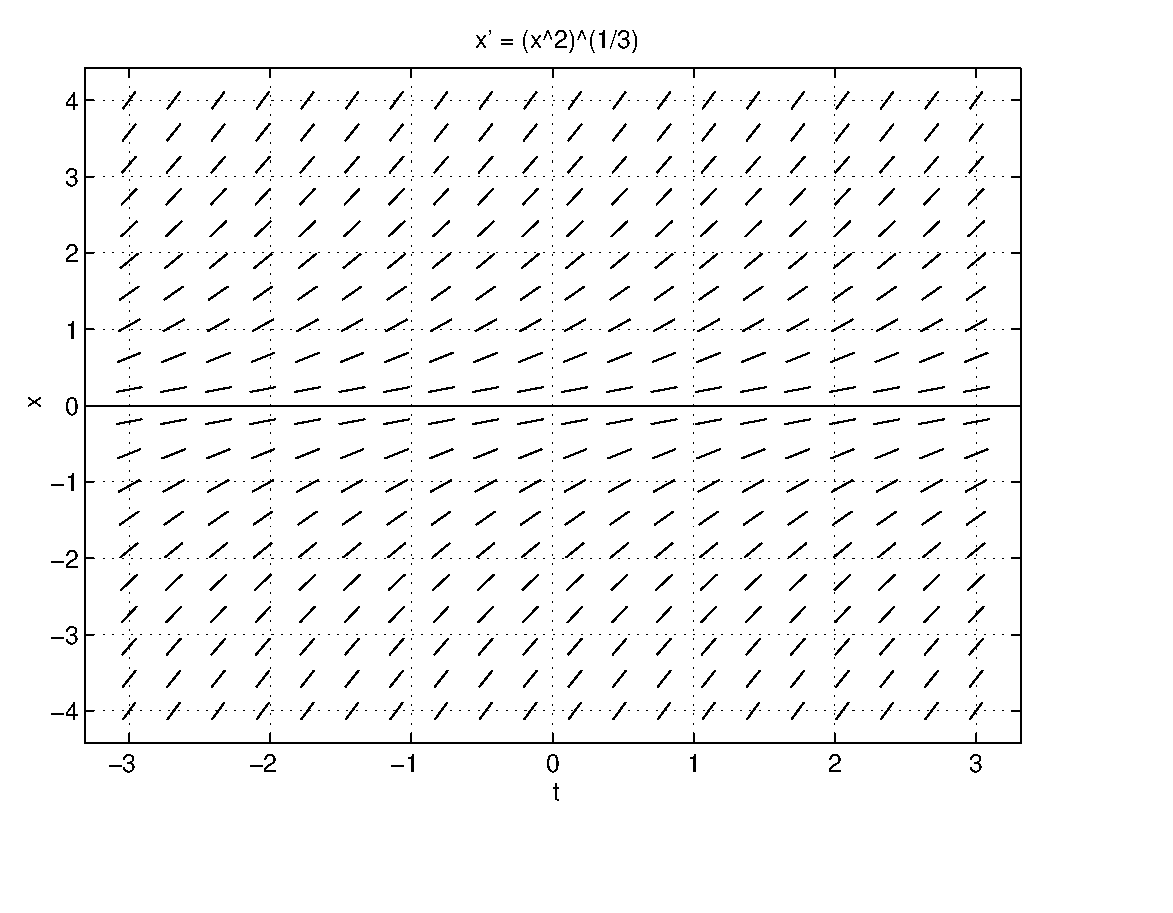
\psfig{file=figures/nonuniqa.eps,width=3.2in}
	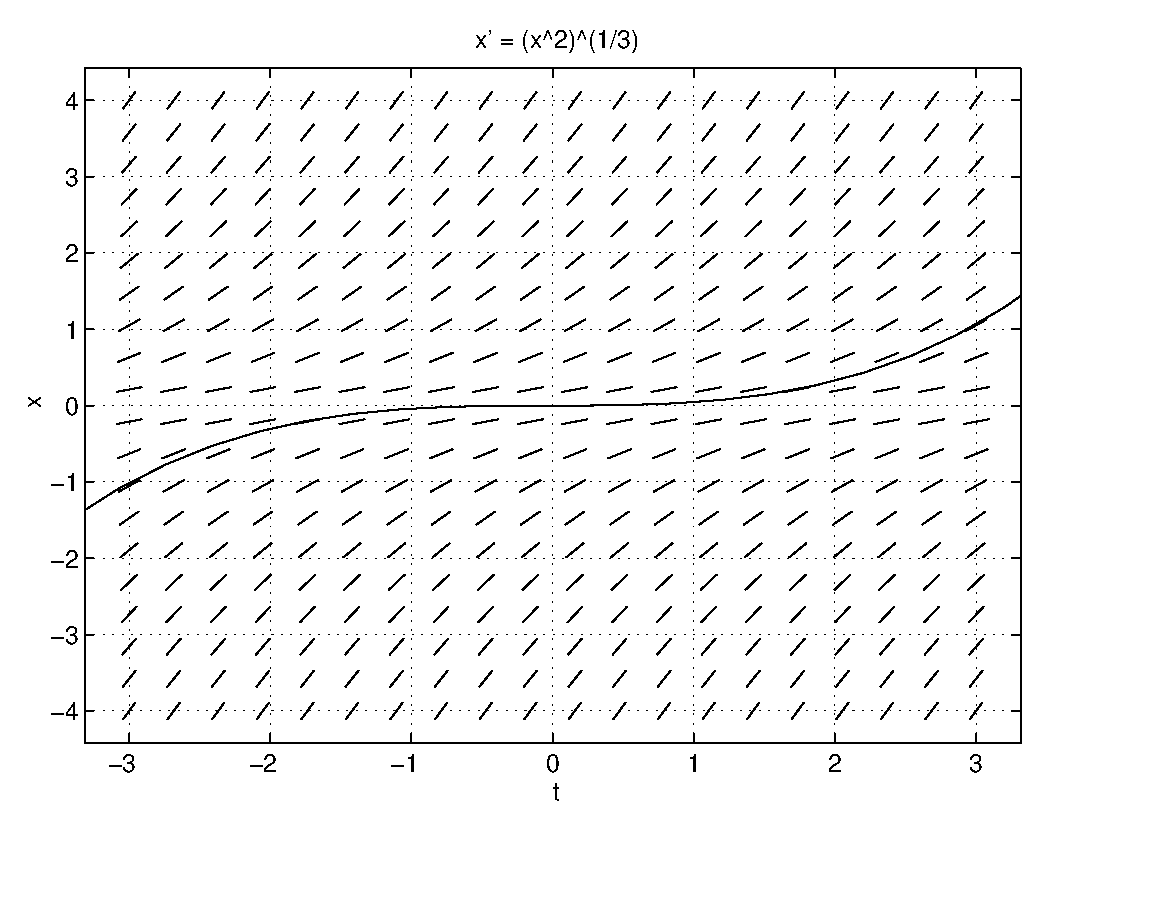
\psfig{file=figures/nonuniqb.eps,width=3.2in}}
        \caption{Solutions for \protect\Ref{nonunique}
              for $t\in [-3,3]$ and $x\in [-4,4]$. Left: $x(0)=0$.
	      Right: $x(0)=0.00001$.}
        \label{nonuniquefig}
\end{figure}

At this stage, we do not have the background to discuss the numerical
method employed by {\sf dfield5}.

\subsection*{The Initial Value Problem for Linear Systems}
\index{initial value problem}

In this chapter we discuss how to find solutions $(x(t),y(t))$ to
\Ref{2dlinsystem} satisfying the initial values $x(0)=x_0$ and $y(0)=y_0$.
It is convenient to rewrite \Ref{2dlinsystem} in matrix form as:
\begin{equation} \label{ndlinsystem}
\frac{dX}{dt}(t) = CX(t).
\end{equation}
The initial value problem is then stated as:  Find a solution to
\Ref{ndlinsystem} satisfying $X(0)=X_0$ where $X_0=(x_0,y_0)^t$.
Everything that we have said here works equally well for $n$
dimensional systems of linear differential equations.  Just let
$C$ be an $n\times n$ matrix and let $X_0$ be an $n$ vector
of initial conditions.

\subsubsection*{Solving the Initial Value Problem Using Superposition}

In Section~\ref{S:IVPR} we discussed how to solve~\Ref{ndlinsystem} when the
eigenvalues of $C$ are real and distinct.  Recall that when $\lambda_1$ and
$\lambda_2$ are distinct real eigenvalues of $C$ with associated
eigenvectors $v_1$ and $v_2$, there are two solutions to \Ref{ndlinsystem}
given by the explicit formulas
\[
X_1(t) = e^{\lambda_1 t}v_1 \AND X_2(t) = e^{\lambda_2 t}v_2.
\]
Superposition guarantees that every linear combination of these solutions
\[
X(t) = \alpha_1X_1(t)+\alpha_2X_2(t) =
\alpha_1e^{\lambda_1 t}v_1 + \alpha_2e^{\lambda_2 t}v_2
\]
is a solution to \Ref{ndlinsystem}.  In addition, we can always choose
scalars $\alpha_1,\alpha_2\in\R$ to solve any given initial value problem
of \Ref{ndlinsystem}.   It follows from the uniqueness of solutions to
initial value problems stated in Theorem~\ref{exist&unique} that all
solutions to \Ref{ndlinsystem} are included in this family of solutions.

We generalize this discussion so that we will be able to find closed form 
solutions to \Ref{ndlinsystem} in Section~\ref{S:TDM} when the eigenvalues 
of $C$ are complex or are real and equal.

Suppose that $X_1(t)$ and $X_2(t)$ are two solutions to \Ref{2dlinsystem} such
that
\[
v_1=X_1(0) \AND v_2=X_2(0)
\]
are linearly independent\index{linearly!independent}.  The existence part of
Theorem~\ref{exist&unique}
guarantees that such solutions exist.  Then all solutions to \Ref{2dlinsystem}
are linear combinations of these two solutions.  We verify this statement as
follows.  Corollary~\ref{C:dim=n} of Chapter~\ref{C:vectorspaces} states
that since $\{v_1,v_2\}$ is a linearly independent set in $\R^2$, it is
also a basis of $\R^2$.  Thus for every $X_0\in\R^2$ there exist scalars
$r_1,r_2$ such that
\[
X_0 = r_1v_1 + r_2v_2.
\]
It follows from superposition and Theorem~\ref{exist&unique} that the
solution
\[
X(t) = r_1X_1(t) + r_2X_2(t)
\]
is the unique solution whose initial condition vector is $X_0$.

We have proved that every solution to this linear system of differential
equations is a linear combination of these two solutions --- that is, we
have proved that the dimension of the space of solutions to \Ref{ndlinsystem}
is two.  This proof generalizes immediately to a proof of the following
theorem for $n\times n$ systems.

\begin{thm}  \label{T:solvends}
Let $C$ be an $n\times n$ matrix.  Suppose that $X_1(t),\ldots,X_n(t)$
are  solutions to $\dot{X}=CX$ such that the vectors of initial conditions
$v_j=X_j(0)$ are linearly independent in $\R^n$.  Then the unique solution
to the system \Ref{ndlinsystem} with initial condition $X(0)=X_0$ is
\begin{equation}  \label{E:genlsoln}
X(t)=r_1X_1(t) + \cdots + r_nX_n(t),
\end{equation}
where $r_1,\ldots,r_n$ are scalars satisfying
\begin{equation} \label{findscalars}
X_0 = r_1v_1 + \cdots + r_nv_n.
\end{equation}
\end{thm}\index{initial condition!linear independence}

We call \Ref{E:genlsoln} the {\em general solution\/} \index{general solution}
to the system of differential equations $\dot{X}=CX$.  When solving the
initial value problem we find a {\em particular solution\/}\index{particular
solution}
by specifying the scalars $r_1,\ldots,r_n$.

\begin{cor}  \label{C:indsoln}
Let $C$ be an $n\times n$ matrix and let ${\cal X}=\{X_1(t),\ldots,X_n(t)\}$
be solutions to the differential equation $\dot{X}=CX$ such that the vectors
$X_j(0)$ are linearly independent in $\R^n$.  Then the set of all solutions
to $\dot{X}=CX$ is an $n$-dimensional subspace of $(\CCone)^n$, and
${\cal X}$ is a basis for the solution subspace.
\end{cor}\index{subspace!of solutions}

Consider a special case of Theorem~\ref{T:solvends}.  Suppose that the
matrix $C$ has $n$ linearly independent eigenvectors $v_1,\ldots,v_n$ with
real eigenvalues $\lambda_1,\ldots,\lambda_n$.  Then the functions
$X_j(t)=e^{\lambda_j t}v_j$ are solutions to $\dot{X}=CX$.
Corollary~\ref{C:indsoln} implies that the functions $X_j$ form a basis for
the space of solutions of this system of differential equations.  Indeed,
the general solution to \Ref{ndlinsystem} is
\begin{equation}  \label{e:gensoln}
X(t) = r_1e^{\lambda_1 t}v_1 + \cdots + r_ne^{\lambda_n t}v_n.
\end{equation}
The particular solution that solves the initial value $X(0)=X_0$ is found by
solving \Ref{findscalars} for the scalars $r_1,\ldots,r_n$.





\EXER

\TEXER

\noindent In Exercises~\ref{c6.1.03a} -- \ref{c6.1.03d}, consider the system of
differential equations
\begin{equation} \label{Ex.1.03}
\begin{array}{rcr}
\frac{dx}{dt}  & = & 65x+42y \\
\frac{dy}{dt}  & = & -99x-64y.
\end{array}
\end{equation}
\begin{exercise} \label{c6.1.03a}
Verify that
\[
v_1 = \vectwo{2}{-3} \AND v_2 = \vectwo{-7}{11}
\]
are eigenvectors of the coefficient matrix of \Ref{Ex.1.03} and find
the associated eigenvalues.
\end{exercise}
\begin{exercise} \label{c6.1.03b}
Find the solution to \Ref{Ex.1.03} satisfying initial conditions $X(0) =
(-14,22)^t$.
\end{exercise}
\begin{exercise} \label{c6.1.03c}
Find the solution to \Ref{Ex.1.03} satisfying initial conditions $X(0) =
(-3,5)^t$.
\end{exercise}
\begin{exercise} \label{c6.1.03d}
Find the solution to \Ref{Ex.1.03} satisfying initial conditions $X(0) =
(9,-14)^t$.
\end{exercise}

\noindent In Exercises~\ref{c6.1.06a} -- \ref{c6.1.06d}, consider the system of
differential equations
\begin{equation} \label{Ex.1.06}
\begin{array}{rcr}
\frac{dx}{dt}  & = & x-y \\
\frac{dy}{dt}  & = & -x+y.
\end{array}
\end{equation}
\begin{exercise} \label{c6.1.06a}
The eigenvalues of the coefficient matrix of \Ref{Ex.1.06} are $0$ and $2$.
Find the associated eigenvectors.
\end{exercise}
\begin{exercise} \label{c6.1.06b}
Find the solution to \Ref{Ex.1.06} satisfying initial conditions
$X(0)=(2,-2)^t$.
\end{exercise}
\begin{exercise} \label{c6.1.06c}
Find the solution to \Ref{Ex.1.06} satisfying initial conditions
$X(0)=(2,6)^t$.
\end{exercise}
\begin{exercise} \label{c6.1.06d}
Find the solution to \Ref{Ex.1.06} satisfying initial conditions
$X(0)=(1,0)^t$.
\end{exercise}


\noindent In Exercises~\ref{c6.1.1a} -- \ref{c6.1.1d}, consider the system of
differential equations
\begin{equation} \label{E:c6.1.1}
\begin{array}{rcr}
\frac{dx}{dt}  & = & -y \\
\frac{dy}{dt}  & = &  x.
\end{array}
\end{equation}
\begin{exercise} \label{c6.1.1a}
Show that $(x_1(t),y_1(t)) = (\cos t,\sin t)$ is a solution to \Ref{E:c6.1.1}.
\end{exercise}
\begin{exercise} \label{c6.1.1b}
Show that $(x_2(t),y_2(t)) = (-\sin t,\cos t)$ is a solution to \Ref{E:c6.1.1}.
\end{exercise}
\begin{exercise} \label{c6.1.1c}
Using Exercises~\ref{c6.1.1a} and \ref{c6.1.1b}, find a solution $(x(t),y(t))$
to \Ref{E:c6.1.1} that satisfies $(x(0),y(0)) = (0,1)$.
\end{exercise}
\begin{exercise} \label{c6.1.1d}
Using Exercises~\ref{c6.1.1a} and \ref{c6.1.1b}, find a solution $(x(t),y(t))$
to \Ref{E:c6.1.1} that satisfies $(x(0),y(0)) = (1,1)$.
\end{exercise}

\noindent In Exercises~\ref{c6.1.2a} -- \ref{c6.1.2b}, consider the system of
differential equations
\begin{equation}  \label{E:c6.1.2}
\begin{array}{rcl}
\frac{dx}{dt} & = & -2x+7y \\
\frac{dy}{dt} & = &  5y,
\end{array}
\end{equation}
\begin{exercise} \label{c6.1.2a}
Find a solution to \Ref{E:c6.1.2}
satisfying the initial condition $(x(0),y(0)) = (1,0)$.
\end{exercise}
\begin{exercise} \label{c6.1.2b}
Find a solution to \Ref{E:c6.1.2}
satisfying the initial condition $(x(0),y(0)) = (-1,2)$.
\end{exercise}

\noindent In Exercises~\ref{c6.1.3a} -- \ref{c6.1.3c}, consider the matrix
\[
C = \left(\begin{array}{rrr} -1 & -10 & -6\\  0 & 4  & 3 \\  0  & -14  & -9
	\end{array}\right).
\]
\begin{exercise} \label{c6.1.3a}
Verify that
\[
v_1 = \left(\begin{array}{r} 1 \\ 0\\ 0\end{array}\right) \qquad
v_2 = \left(\begin{array}{r} 2 \\ -1\\ 2\end{array}\right) \quad \AND \quad
v_3 = \left(\begin{array}{r} 6 \\ -3\\ 7\end{array}\right)
\]
are eigenvectors of $C$ and find the associated eigenvalues.
\end{exercise}
\begin{exercise} \label{c6.1.3b}
Find a solution to the system of differential equations
$\dot{X}=CX$ satisfying the initial condition $X(0)= (10, -4, 9)^t$.
\end{exercise}
\begin{exercise} \label{c6.1.3c}
Find a solution to the system of differential equations
$\dot{X}=CX$ satisfying the initial condition $X(0)= ( 2, -1, 3)^t$.
\end{exercise}

\begin{exercise}  \label{c6.1.4A}
Show that for some nonzero $a$ the function $x(t)=at^5$ is a solution to the
differential equation $\dot{x}=x^{4/5}$.  Then show that there are at least
two solutions to the initial value problem $x(0)=0$ for this differential
equation.
\end{exercise}


\CEXER

\begin{exercise} \label{c6.1.4}
Use {\sf pplane5}\index{\computer!pplane5} to investigate the system
of differential equations
\begin{equation}  \label{Ex.1.4}
\begin{array}{rcr}
\frac{dx}{dt}  & = & -2y \\
\frac{dy}{dt}  & = &  -x+y.
\end{array}
\end{equation}
\begin{itemize}
\item[(a)] Use {\sf pplane5} to find two independent eigendirections (and
hence eigenvectors) for \Ref{Ex.1.4}.
\item[(b)] Using (a), find the eigenvalues of the coefficient matrix of
\Ref{Ex.1.4}.
\item[(c)] Find a closed form solution to \Ref{Ex.1.4} satisfying the initial
condition
\[
X(0) = \vectwo{4}{-1}.
\]
\item[(d)] Study the time series of $y$ versus $t$ for the solution in (c)
by comparing the graph of the closed form solution obtained in (c) with the
time series graph using {\sf pplane5}.
\end{itemize}
\end{exercise}




\section{Closed Form Solutions by the Direct Method}
\label{S:TDM}


In Section~\ref{S:IVPR} we showed in detail how solutions to planar systems
of constant coefficient differential equations with distinct real eigenvalues
are found.  This method was just reviewed in Section~\ref{S:6.1} where we saw
that the crucial step in solving these systems of differential equations is
the step where we find two linearly independent solutions.   In this section
we discuss how to find these two linearly independent solutions when the
eigenvalues of the coefficient matrix are either complex or real and equal.

By finding these two linearly independent solutions we will find both
the {\em general\/} solution of the system of differential equations
$\dot{X}=CX$ and a method for solving the initial value
problem\index{initial value problem}
\begin{equation}  \label{e:eqnA}
\begin{array}{rcl}
\dps\frac{dX}{dt} & = & CX\\
X(0) & = & X_0.
\end{array}
\end{equation}
We assume that $C$ is a $2\times 2$ matrix with eigenvalues $\lambda_1$ and
$\lambda_2$.  When needed, we denote the associated eigenvectors by $v_1$ and
$v_2$.

\subsection*{Real Distinct Eigenvalues}
\index{eigenvalue!real}

We have discussed the case when $\lambda_1\neq\lambda_2\in\R$ on several
occasions.  For completeness we repeat the result.  The general solution is:
\begin{equation}  \label{E:RD2}
X(t) = \alpha_1 e^{\lambda_1 t}v_1 + \alpha_2 e^{\lambda_2 t}v_2.
\end{equation}
The initial value problem is solved by finding real numbers $\alpha_1$ and
$\alpha_2$ such that
\[
X_0 = \alpha_1 v_1 + \alpha_2 v_2.
\]
See Section~\ref{S:IVPR} for a detailed discussion with examples.

\subsection*{Complex Conjugate Eigenvalues}
\index{eigenvalue!complex}

Suppose that the eigenvalues of $C$ are complex, that is, suppose that
$\lambda_1= \sigma+i\tau$ with $\tau\neq 0$ is an eigenvalue of $C$ with
eigenvector $v_1=v+iw$, where $v,w\in\R^2$.  We claim that
$X_1(t)$ and $X_2(t)$, where
\begin{equation}  \label{E:CC1}
\begin{array}{rcl}
X_1(t) & = & e^{\sigma t}(\cos(\tau t)v -\sin(\tau t)w)\\
X_2(t) & = & e^{\sigma t}(\sin(\tau t)v +\cos(\tau t)w),
\end{array}
\end{equation}
are solutions to \Ref{e:eqnA} and that the general
solution\index{general solution} to \Ref{e:eqnA} is:
\begin{equation}  \label{E:CC2}
X(t) = \alpha_1 X_1(t) + \alpha_2 X_2(t),
\end{equation}
where $\alpha_1, \alpha_2$ are real scalars.

There are several difficulties in deriving \Ref{E:CC1} and \Ref{E:CC2}; these
difficulties are related to using complex numbers as opposed to real numbers.
In particular, in the derivation of \Ref{E:CC1} we need to define the
exponential of a complex number, and we begin by discussing this issue.

\subsubsection*{Euler's Formula}\index{Euler's formula}

We find complex exponentials by using Euler's celebrated formula:
\begin{equation}  \label{E:Euler}
e^{i\theta} = \cos\theta + i\sin\theta
\end{equation}
for any real number $\theta$.  A justification of this formula is
given in Exercise~\ref{c6.6.05}.   Euler's formula allows us to differentiate
complex exponentials, obtaining the expected result:
\begin{eqnarray*}
\frac{d}{dt}e^{i\tau t} & = &
\frac{d}{dt}(\cos(\tau t) + i\sin(\tau t))\\
& = & \tau(-\sin(\tau t) + i\cos(\tau t)) \\
& = & i\tau(\cos(\tau t) + i\sin(\tau t))\\
& = & i\tau e^{i\tau t}.
\end{eqnarray*}

Euler's formula also implies that
\begin{equation}  \label{E:ecis}
e^{\lambda t} = e^{\sigma t + i\tau t} = e^{\sigma t}e^{i\tau t} =
e^{\sigma t}(\cos(\tau t) + i\sin(\tau t)),
\end{equation}
where $\lambda = \sigma+i\tau$.  Most importantly, we note that
\begin{equation}  \label{E:eldiff}
\frac{d}{dt}e^{\lambda t} = \lambda e^{\lambda t}.
\end{equation}
We use \Ref{E:ecis} and the product rule for differentiation to verify
\Ref{E:eldiff} as follows:
\begin{eqnarray*}
\frac{d}{dt}e^{\lambda t} & =  &
\frac{d}{dt}\left(e^{\sigma t}e^{i\tau t}\right)\\
& = & \left(\sigma e^{\sigma t}\right)e^{i\tau t}
+ e^{\sigma t}\left(i\tau e^{i\tau t}\right)\\
& = & (\sigma+i\tau)e^{\sigma t + i\tau t} \\
& = & \lambda e^{\lambda t}.
\end{eqnarray*}

\subsubsection*{Verification that \protect\Ref{E:CC2} is the General Solution}

A complex vector-valued function $X(t)=X_1(t)+iX_2(t)\in\C^n$
\index{complex valued solution} consists of
a {\em real part\/} $X_1(t)\in\R^n$ and an {\em imaginary part\/}
\index{complex valued solution!real part}
\index{complex valued solution!imaginary part}
$X_2(t)\in\R^n$.  For such functions $X(t)$ we define
\[
\dot{X} = \dot{X}_1+i\dot{X}_2
\]
and
\[
CX = CX_1 + iCX_2.
\]
To say that $X(t)$ is a solution to $\dot{X}=CX$ means that
\begin{equation}  \label{E:X1X2}
\dot{X}_1+i\dot{X}_2 = \dot{X} = CX = CX_1 + iCX_2.
\end{equation}

\begin{lemma}  \label{L:RIsoln}
The complex vector-valued function $X(t)$ is a solution to $\dot{X}=CX$ if
and only if the real and imaginary parts are real vector-valued solutions
to $\dot{X}=CX$.
\end{lemma}

\begin{proof} Equating the real and imaginary parts of \Ref{E:X1X2} implies that
\[
\dot{X}_1 = CX_1 \AND \dot{X}_2 = CX_2.
\]
\end{proof}

It follows from Lemma~\ref{L:RIsoln} that finding one complex-valued solution
to a linear differential equation provides us with two real-valued solutions.
Identity \Ref{E:eldiff} implies that
\[
X(t) = e^{\lambda_1 t}v_1
\]
is a complex-valued solution to \Ref{e:eqnA}.  Using Euler's formula we
compute the real and imaginary parts of $X(t)$, as follows.
\begin{eqnarray*}
X(t) & = & e^{(\sigma+i\tau)t}(v+iw) \\
& = & e^{\sigma t} (\cos(\tau t)+i\sin(\tau t))(v+iw)\\
& = & e^{\sigma t}(\cos(\tau t)v-\sin(\tau t)w)+
ie^{\sigma t}(\sin(\tau t)v+\cos(\tau t)w).
\end{eqnarray*}
Since the real and imaginary parts of $X(t)$ are solutions to $\dot{X}=CX$, it
follows that the real-valued functions $X_1(t)$ and $X_2(t)$ defined in
\Ref{E:CC1} are indeed solutions.

Returning to the case where $C$ is a $2\times 2$ matrix, we see that if
$X_1(0)=v$ and $X_2(0)=w$ are linearly independent, then
Corollary~\ref{C:indsoln} implies that \Ref{E:CC2} is the general solution to
$\dot{X}=CX$.  The linear independence of $v$ and $w$ is verified using the
following lemma.

\begin{lemma}  \label{L:rievind}
Let $\lambda_1=\sigma+i\tau$ with $\tau\neq 0$ be a
complex eigenvalue\index{eigenvalue!complex} of the
$2\times 2$ matrix $C$ with eigenvector\index{eigenvector}
$v_1=v+iw$ where $v,w\in\R^2$.  Then
\begin{equation}  \label{e:complexcoord}
\begin{array}{rcl}
Cv & = & \sigma v - \tau w \\
Cw & = & \tau v + \sigma w.
\end{array}
\end{equation}
and $v$ and $w$ are linearly independent\index{linearly!independent} vectors.
\end{lemma}

\begin{proof}   By assumption $Cv_1=\lambda_1v_1$, that is,
\begin{equation}  \label{E:viw}
C (v+iw) = (\sigma+i\tau)(v+iw) = (\sigma v - \tau w) + i(\tau v + \sigma w).
\end{equation}
Equating real and imaginary parts of \Ref{E:viw} leads to the system of
equations \Ref{e:complexcoord}.  Note that if $w=0$, then $v\neq 0$ and
$\tau v = 0$.  Hence $\tau=0$, contradicting the assumption that
$\tau\neq 0$.  So $w\neq 0$.

Note also that if $v$ and $w$ are linearly dependent, then $v=\alpha w$.
It then follows from the previous equation that
\[
Cw = (\tau\alpha+\sigma)w.
\]
Hence $w$ is a real eigenvector; but the eigenvalues of $C$ are not real and
$C$ has no real eigenvectors.   \end{proof}


\subsubsection*{An Example with Complex Eigenvalues}

Consider an example of an initial value problem for a linear system with
complex eigenvalues.  Let
\begin{equation}  \label{e:complexexample}
\frac{dX}{dt} = \mattwo{-1}{2}{-5}{-3} X = CX,
\end{equation}
and
\[
X_0=\vectwo{1}{1}.
\]

The characteristic polynomial\index{characteristic polynomial} for the
matrix $C$ is:
\[
p_C(\lambda) = \lambda^2 +4\lambda + 13,
\]
whose roots are $\lambda_1 = -2+3i$ and $\lambda_2 = -2-3i$. So
\[
\sigma = -2 \AND \tau = 3.
\]
An eigenvector corresponding to the eigenvalue $\lambda_1$ is
\[
v_1 = \vectwoc{2}{-1+3i} = \vectwo{2}{-1}+i\vectwo{0}{3}=v+iw.
\]
It follows from \Ref{E:CC1} that
\[
\begin{array}{rcl}
X_1(t) & = & e^{-2t}(\cos(3t)v -\sin(3t)w)\\
X_2(t) & = & e^{-2t}(\sin(3t)v +\cos(3t)w),
\end{array}
\]
are solutions to \Ref{e:complexexample} and $X=\alpha_1X_1+\alpha_2X_2$ is
the general solution to \Ref{e:complexexample}.  To solve the initial value
problem we need to find $\alpha_1,\alpha_2$ such that
\[
X_0 = X(0) = \alpha_1X_1(0) + \alpha_2X_2(0) = \alpha_1 v + \alpha_2 w,
\]
that is,
\[
\vectwo{1}{1} = \alpha_1\vectwo{2}{-1}  + \alpha_2\vectwo{0}{3}.
\]
Therefore, $\alpha_1 = \frac{1}{2}$ and $\alpha_2=\frac{1}{2}$ and
\begin{equation}  \label{e:complexexampleans}
X(t) =  e^{-2t}\vectwoc{\cos(3t)+\sin(3t)}{\cos(3t)-2\sin(3t)}.
\end{equation}

\subsection*{Real and Equal Eigenvalues}

There are two types of $2\times 2$ matrices that have real and equal
\index{eigenvalue!real!equal}
eigenvalues --- those that are scalar multiples of the identity and those
that are not.  An example of a $2\times 2$ matrix that has real and equal
eigenvalues is
\begin{equation}  \label{E:equalex}
A = \mattwoc{\lambda_1}{1}{0}{\lambda_1}, \quad \lambda_1\in\R.
\end{equation}
The characteristic polynomial of $A$ is
\[
p_A(\lambda) = \lambda^2 - \trace(A)\lambda + \det(A) =
\lambda^2 -2\lambda_1\lambda + \lambda_1^2 = (\lambda-\lambda_1)^2.
\]
Thus the eigenvalues of $A$ both equal $\lambda_1$.

\subsubsection*{Only One Linearly Independent Eigenvector}

An important fact about the matrix $A$ in \Ref{E:equalex} is that it has
only one linearly independent eigenvector.  To verify this fact, solve the
system of linear equations
\[
Av = \lambda_1v.
\]
In matrix form this equation is
\[
0 = (A-\lambda_1I_2)v = \mattwo{0}{1}{0}{0}v.
\]
A quick calculation shows that all solutions are multiples of
$v_1=e_1=(1,0)^t$.

In fact, this observation is valid for any $2\times 2$ matrix that has
equal eigenvalues and is not a scalar multiple of the identity, as the next
lemma shows.

\begin{lemma}  \label{L:1indeig}
Let $A$ be a $2\times 2$ matrix.  Suppose that $A$ has two linearly
independent eigenvectors both with eigenvalue $\lambda_1$.
Then $A=\lambda_1 I_2$.
\end{lemma}\index{eigenvector!linearly independent}\index{eigenvector!real}

\begin{proof}  Let $v_1$ and $v_2$ be two linearly independent
eigenvectors of $A$, that is, $Av_j = \lambda_1 v_j$.  It follows
from linearity that $Av=\lambda_1 v$ for any linear combination
$v=\alpha_1v_1+\alpha_2v_2$.  Since $v_1$ and $v_2$ are linearly
independent and $\dim(\R^2)=2$, it follows that $\{v_1,v_2\}$ is
a basis of $\R^2$.  Thus, every vector $v\in\R^2$ is a linear
combination of $v_1$ and $v_2$.  Therefore, $A$ is $\lambda_1$ times
the identity matrix.  \end{proof}

\subsubsection*{Generalized Eigenvectors}

Suppose that $C$ has exactly one linearly independent real eigenvector $v_1$
with real eigenvalue $\lambda_1$.  We call $w_1$ a {\em generalized
eigenvector\/}\index{eigenvector!generalized} of $C$ it satisfies the
system of linear equations
\begin{equation} \label{e:Cw=lw+va}
(C-\lambda_1I_2)w_1 = v_1.
\end{equation}

The matrix $A$ in \Ref{E:equalex} has a generalized eigenvector. To verify
this point solve the linear system
\[
(A-\lambda_1I_2)w_1 = \mattwo{0}{1}{0}{0}w_1 = v_1 = \vectwo{1}{0}
\]
for $w_1=e_2$.   Note that for this matrix $A$, $v_1=e_1$ and $w_1=e_2$ are
linearly independent.  The next lemma shows that this observation about
generalized eigenvectors is always valid.

\begin{lemma}  \label{L:geneig2}
Let $C$ be a $2\times 2$ matrix with both eigenvalues equal to $\lambda_1$
and with one linearly independent eigenvector $v_1$.  

\noindent (a)  Let $w_1$ be a generalized eigenvector of $C$, then $v_1$ and 
$w_1$ are linearly independent. 

\noindent (b)  Let $w$ be any vector such that $v_1$ and $w$ are linearly 
independent.  Then $w$ is a nonzero scalar multiple of a generalized 
eigenvector of $C$.
\end{lemma}

\begin{proof}  (a) If $v_1$ and $w_1$ were linearly dependent, then $w_1$ would be 
a multiple of $v_1$ and hence an eigenvector of $C$.  But $C-\lambda_1I_2$
applied to an eigenvector is zero, which is a contradiction.  Therefore, 
$v_1$ and $w_1$ are linearly independent.

(b) Let $w$ be any vector that is linearly independent of
the eigenvector $v_1$.  It follows that  $\{v_1,w\}$ is a basis for
$\R^2$; hence
\begin{equation} \label{E:Cw1}
Cw = \alpha v_1 + \beta w
\end{equation}
for some scalars $\alpha$ and $\beta$.    If $\alpha=0$, then
$w$ is an eigenvector of $C$, contradicting the assumption that $C$ has
only one linearly independent eigenvector.  Therefore, $\alpha\neq 0$.

We claim that $\beta=\lambda_1$ and we prove the claim by showing that
$\beta$ is an eigenvalue of $C$.  Hence $\beta$ must equal $\lambda_1$
since both eigenvalues of $C$ equal $\lambda_1$.  To see that $\beta$
is an eigenvalue, define the nonzero vector
\[
u = \alpha v_1 +(\beta-\lambda_1)w
\]
and compute
\[
Cu = \lambda_1 \alpha v_1 + (\beta-\lambda_1)(\alpha v_1+\beta w) =
\beta u.
\]
So $u$ is an eigenvector of $C$ with eigenvalue $\beta$.
It now follows from \Ref{E:Cw1} that
\[
(C-\lambda_1I_2)w = \alpha v_1.
\]
Therefore, $w_1=\frac{1}{\alpha}w$ is a generalized eigenvector
of $C$.  \end{proof}



\subsubsection*{Independent Solutions to Differential Equations with
Equal Eigenvalues}

In the equal eigenvalue one eigenvector case, we
claim that the general solution\index{general solution} to $\dot{X}=CX$ is:
\begin{equation}  \label{e:exp1eva}
X(t) = e^{\lambda_1 t}\left(\alpha v_1 +\beta (w_1+tv_1)\right),
\end{equation}
where $v_1$ is an eigenvector of $C$ and $w_1$ is the generalized
eigenvector.

Since $v_1$ is an eigenvector of $C$ with eigenvalue $\lambda_1$, the
function $X_1(t)=e^{\lambda_1 t}v_1$ is a solution to $\dot{X}=CX$.  Suppose
that we can show that $X_2(t)=e^{\lambda_1 t}(w_1+tv_1)$ is also a solution
to $\dot{X}=CX$.  Then \Ref{e:exp1eva} is the general solution, since
$X_1(0)=v_1$ and $X_2(0)=w_1$ are linearly independent by 
Lemma~\ref{L:geneig2}(a).  Apply Theorem~\ref{T:solvends}.

To verify that $X_2(t)$ is a solution (that is, that $\dot{X}_2=CX_2$),
calculate
\[
\dot{X}_2(t) = \lambda_1 e^{\lambda_1 t}(w_1+tv_1) + e^{\lambda_1 t}v_1=
e^{\lambda_1 t}(\lambda_1 w_1 + v_1 +t\lambda v_1)
\]
and
\[
CX_2(t) = e^{\lambda_1 t}(Cw_1+tCv_1) = e^{\lambda_1 t}
((v_1+\lambda_1 w_1)+t\lambda_1 v_1),
\]
using \Ref{e:Cw=lw+va}.  Note that $X(0)=\alpha v_1 + \beta w_1$, so $\alpha$
and $\beta$ are found by solving $X_0= \alpha v_1 + \beta w_1$.

\subsubsection*{An Example with Equal Eigenvalues}

Consider the system of differential equations
\begin{equation}  \label{e:shearexample}
\frac{dX}{dt} = \mattwo{1}{-1}{9}{-5} X
\end{equation}
with initial value
\[
X_0 = \vectwo{2}{3}.
\]
The characteristic polynomial for the matrix $C=\mattwo{1}{-1}{9}{-5}$ is
\[
p_C(\lambda) = \lambda^2 + 4\lambda +4 = (\lambda + 2)^2.
\]
Thus $\lambda_1=-2$ is an eigenvalue of multiplicity two.  Since
$C$ is not a multiple of the identity matrix, it must have
precisely one linearly independent eigenvector $v_1$.  This eigenvector is
found by solving the equation
\[
0 = (C-\lambda_1I_2)v_1 = (C+2I_2)v_1 = \mattwo{3}{-1}{9}{-3}v_1
\]
for
\[
v_1=\vectwo{1}{3}.
\]
To find the generalized eigenvector $w_1$, we solve the system of linear
equations
\[
(C-\lambda_1I_2)w_1=(C+2I_2)w_1=\mattwo{3}{-1}{9}{-3}w_1= v_1=\vectwo{1}{3}
\]
by row reducing the augmented matrix
\[
\left(\begin{array}{rr|r} 3 & -1 & 1\\ 9 & -3 & 3 \end{array}\right)
\]
to obtain
\[
w_1 = \vectwo{1}{2}.
\]

We may now apply \Ref{e:exp1eva} to find the general solution to
\Ref{e:shearexample}
\[
X(t) = e^{-2t}\left(\alpha v_1 +\beta (w_1+tv_1)\right).
\]
We solve the initial value problem by solving
\[
\vectwo{2}{3} = X_0 = X(0) = \alpha v_1 +\beta w_1 =
\mattwo{1}{1}{3}{2}\vectwo{\alpha}{\beta}
\]
for $\alpha=-1$ and $\beta=3$.   So the closed form solution to this initial
value problem is
\begin{eqnarray*}
X(t) & = & e^{-2t}\left(-v_1 + 3(w_1+tv_1)\right)\\
& = & e^{-2t}\left(-\vectwo{1}{3}+3\vectwoc{1+t}{2+3t}\right)\\
& = & e^{-2t}\vectwo{2+3t}{3+9t}.
\end{eqnarray*}

There is a simpler method for finding this solution --- a method that
does not require solving for either the eigenvector $v_1$ or the generalized
eigenvector $w_1$ that we will discuss later.  See Section~\ref{S:6.6}.

\EXER

\TEXER

\begin{exercise}  \label{c6.6.05}
Justify Euler's formula \Ref{E:Euler} as follows.  Recall the
Taylor series
\begin{eqnarray*}
e^x & = & 1 + x + \frac{1}{2!}x^2 + \cdots + \frac{1}{n!}x^n + \cdots\\
\cos x & = & 1 - \frac{1}{2!}x^2 + \frac{1}{4!}x^4 + \cdots +
(-1)^n \frac{1}{(2n)!}x^{2n} + \cdots \\
\sin x & = & x - \frac{1}{3!}x^3 + \frac{1}{5!}x^5 + \cdots +
(-1)^n \frac{1}{(2n+1)!}x^{2n+1} + \cdots.
\end{eqnarray*}
Now evaluate the Taylor series $e^{i\theta}$ and separate into real and
imaginary parts.
\end{exercise}

 In modern language De Moivre's formula states that
\[
e^{ni\theta} = \left(e^{i\theta}\right)^n.
\]
In Exercises~\ref{c6.6.1a} -- \ref{c6.6.1b} use De Moivre's formula coupled
with Euler's formula \Ref{E:Euler} to determine trigonometric identities
for the given quantity in terms of $\cos\theta$, $\sin\theta$, $\cos\varphi$,
$\sin\varphi$.
\begin{exercise}  \label{c6.6.1a}
$\cos(\theta+\varphi)$.
\end{exercise}
\begin{exercise}  \label{c6.6.1b}
$\sin(3\theta)$.
\end{exercise}

In Exercises~\ref{c6.6.2a} -- \ref{c6.6.2d} compute the general solution for
the given system of differential equations.
\begin{exercise}  \label{c6.6.2a}
$\dps\frac{dX}{dt} = \mattwo{-1}{-4}{2}{3} X$.
\end{exercise}
\begin{exercise}  \label{c6.6.2b}
$\dps\frac{dX}{dt} = \mattwo{8}{-15}{3}{-4} X$.
\end{exercise}
\begin{exercise}  \label{c6.6.2c}
$\dps\frac{dX}{dt} = \mattwo{5}{-1}{1}{3} X$.
\end{exercise}
\begin{exercise}  \label{c6.6.2d}
$\dps\frac{dX}{dt} = \mattwo{-4}{4}{-1}{0} X$.
\end{exercise}

\section{Solutions Using Matrix Exponentials}
\label{S:Matrixexp} \index{matrix!exponential}

In Section~\ref{S:growthmodels} we showed that the solution of the single
ordinary differential equation $\dot x(t) = \lambda x(t)$ with initial
condition $x(0)=x_0$ is $x(t) = e^{t\lambda}x_0$ (see \Ref{lin1} in
Chapter~\ref{chap:SolveOdes}).  In this section we show that we
may write solutions of systems of equations in a similar form.
In particular, we show that the solution to the linear system of ODEs
\begin{equation}   \label{eq:x=Mx}
\frac{dX}{dt} = CX
\end{equation}
with initial condition
\[
X(0) = X_0,
\]
where $C$ is an $n\times n$ matrix and $X_0\in\R^n$, is
\begin{equation}  \label{matrixsoln}
X(t) = e^{tC}X_0.
\end{equation}

In order to make sense of the solution \Ref{matrixsoln} we need
to understand matrix exponentials. More precisely, since $tC$ is
an $n\times n$ matrix for each $t\in\R$, we need to make sense
of the expression $e^L$ where $L$ is an $n\times n$ matrix.  For
this we recall the form of the exponential function as a power
series:
\[
     e^t = 1 + t + \frac{1}{2!} t^2 + \frac{1}{3!} t^3
     + \frac{1}{4!} t^4 + \cdots .
\]
In more compact notation we have
\[
     e^t = \sum\limits_{k=0}^\infty \frac{1}{k!} t^k.
\]
By analogy, define the {\em matrix exponential\/}\index{matrix!exponential}
$e^L$ by
\begin{eqnarray}
e^{L} & = & I_n + L + \frac{1}{2!} L^2 + \frac{1}{3!} L^3 +\cdots
\label{e:expL}\\
      & = & \sum\limits_{k=0}^\infty\frac{1}{k!} L^k. \nonumber
\end{eqnarray}
In this formula $L^2 = LL$ is the matrix product of $L$ with itself, and the
power $L^k$ is defined inductively by $L^k = LL^{k-1}$ for $k>1$.  Hence
$e^L$ is an $n\times n$ matrix and is the infinite sum of $n\times n$
matrices.

\noindent {\bf Remark:}   The infinite series for matrix exponentials
\Ref{e:expL} does converge for all $n\times n$ matrices $L$, and this fact
is proved in Exercises~\ref{c6.2.7} and \ref{c6.2.8}.

Using \Ref{e:expL}, we can write the matrix exponential of $tC$
for each real number $t$.  Since $(tC)^k = t^k C^k$ we obtain
\arraystart
\begin{equation}  \label{eq:MatrixExp}
\begin{array}{rcl}
\dps e^{tC} & = & \dps I_n + tC + \frac{1}{2!} (tC)^2 + \frac{1}{3!} (tC)^3
+\cdots\\
\dps & = & \dps I_n + tC + \frac{t^2}{2!} C^2 + \frac{t^3}{3!} C^3 +\cdots.
\end{array}
\end{equation}
\arrayfinish
Next we claim that
\begin{equation}  \label {e:diffmatexp}
  \frac{d}{dt} e^{tC} = Ce^{tC}.
\end{equation}
We verify the claim by supposing that we can differentiate
\Ref{eq:MatrixExp} term by term with respect to $t$. Then
\begin{eqnarray*}
  \dps\frac{d}{dt} e^{tC} & = & \frac{d}{dt}(I_n) + \frac{d}{dt}(tC)
  + \frac{d}{dt}\left(\frac{t^2}{2!} C^2\right) +
  \frac{d}{dt}\left(\frac{t^3}{3!} C^3\right) +
  \frac{d}{dt}\left(\frac{t^4}{4!}C^4\right) + \cdots\\
     & = & 0 + C + t C^2 + \frac{t^2}{2!} C^3 +
\frac{t^3}{3!} C^4 + \cdots\\
     & = & C\left(I_n + tC + \frac{t^2}{2!} C^2 + \frac{t^3}{3!} C^3
+\cdots\right)\\
     & = & Ce^{tC}.
\end{eqnarray*}
It follows that the function $X(t) = e^{tC}X_0$ is a solution of
\Ref{eq:x=Mx} for each $X_0\in\R^n$; that is,
\[
     \frac{d}{dt} X(t) =  \frac{d}{dt}  e^{tC}X_0
     = C e^{tC}X_0 = C X(t).
\]
Since \Ref{e:expL} implies that $e^{0C} = e^0 = I_n$, it follows
that $X(t) = e^{tC}X_0$ is a solution of \Ref{eq:x=Mx} with
initial condition $X(0)=X_0$.  This discussion shows that solving
\Ref{eq:x=Mx} in closed form is equivalent to finding a closed
form expression for the matrix exponential $e^{tC}$.

\begin{thm}  \label{T:linODEsoln}
The unique solution\index{uniqueness of solutions} to the
initial value problem\index{initial value problem}
\arraystart
\[
\begin{array}{rcl}
\dps\frac{dX}{dt} & = & CX \\
X(0) & = & X_0
\end{array}
\]
\arrayfinish
is
\[
X(t)=e^{tC}X_0.
\]
\end{thm}

\begin{proof}  Existence follows from the previous discussion;
uniqueness follows from the $n$ dimensional analog of
Theorem~\ref{exist&unique}.  \end{proof}


\subsection*{Explicit Computation of Matrix Exponentials}
\index{matrix!exponential!computation}

We begin with the simplest computation of a matrix exponential.

\noindent (a) \quad Let $L$ be a multiple of the identity; that
is, let $L = \alpha I_n$ where $\alpha$ is a real number.  Then
\begin{equation} \label{ex:expm}
e^{\alpha I_n} = e^{\alpha} I_n.
\end{equation}
That is, $e^{\alpha I_n}$ is a scalar multiple of the
identity.  To verify \Ref{ex:expm}, compute
\[
e^{\alpha I_n} = I_n + \alpha I_n + \frac{\alpha^2}{2!} I_n^2 +
\frac{\alpha^3}{3!} I_n^3 +\cdots = (1+\alpha+\frac{\alpha^2}{2!}
+\frac{\alpha^3}{3!}+\cdots)I_n = e^{\alpha} I_n.
\]

\noindent (b) \quad Let $C$ be a $2\times 2$ diagonal matrix,
     \[
          C = \mattwo{\lambda_1}{0}{0}{\lambda_2},
     \]
where $\lambda_1$ and $\lambda_2$ are real constants.  Then
\begin{equation}  \label{e:expdiag}
e^{tC} = \mattwo{e^{\lambda_1 t}}{0}{0}{e^{\lambda_2 t}}.
\end{equation}
To verify \Ref{e:expdiag} compute
\begin{eqnarray*}
   e^{tC} & = & I_2 + tC + \frac{t^2}{2!} C^2 +  \frac{t^3}{3!} C^3 +\cdots\\
        & = & \mattwo{1}{0}{0}{1} + \mattwo{\lambda_1 t}{0}{0}{\lambda_2 t} +
\mattwo{\frac{t^2}{2!}\lambda_1^2}{0}{0}{\frac{t^2}{2!}\lambda_2^2} +\cdots\\
        & = & \mattwo{e^{\lambda_1 t}}{0}{0}{e^{\lambda_2 t}}.
\end{eqnarray*}

\noindent (c) \quad Suppose that
     \[
                C = \mattwo{0}{-1}{1}{0}.
      \]
Then
\begin{equation} \label{e:exprotate}
e^{tC} = \mattwo{\cos t}{-\sin t}{\sin t}{\cos t}.
\end{equation}
We begin this computation by observing that
\[
C^2 = -I_2, \quad C^3 = -C, \AND C^4 = I_n.
\]
Therefore, by collecting terms of odd and even power in the series
expansion for the matrix exponential we obtain
\begin{eqnarray*}
e^{tC} & = & I_2 + tC + \frac{t^2}{2!} C^2 +  \frac{t^3}{3!}C^3 +\cdots\\
     & = & I_2 + tC - \frac{t^2}{2!}I_2 - \frac{t^3}{3!}C +\cdots\\
     & = & \left(1 - \frac{t^2}{2!} + \frac{t^4}{4!} - \frac{t^6}{6!} +
		\cdots \right)I_2
	 + \left(t - \frac{t^3}{3!} + \frac{t^5}{5!} - \frac{t^7}{7!} +
	\cdots \right)C \\
     & = & (\cos t)I_2 + (\sin t)C \\
     & = & \mattwo{\cos t}{-\sin t}{\sin t}{\cos t}.
     \end{eqnarray*}
In this computation we have used the fact that the trigonometric
functions $\cos t$ and $\sin t$ have the power series expansions:
\begin{eqnarray*}
\cos t & = & 1-\frac{1}{2!}t^2+\frac{1}{4!} t^4 + \cdots =
\sum\limits_{k=0}^\infty\frac{(-1)^k}{(2k)!} t^{2k},\\
\sin t & = & t-\frac{1}{3!} t^3 + \frac{1}{5!} t^5 + \cdots
   = \sum\limits_{k=0}^\infty \frac{(-1)^k}{(2k+1)!} t^{2k+1}.
\end{eqnarray*}
See Exercise~\ref{c6.2.5C} for an alternative proof of \Ref{e:exprotate}.

To compute the matrix exponential
\Matlab\index{matrix!exponential!in \protect\Matlab} provides the command
{\tt expm}\index{\computer!expm}.  We use this command to compute
the matrix exponential $e^{tC}$ for
\[
C=\mattwo{0}{-1}{1}{0} \AND t=\frac{\pi}{4}.
\]
Type
\begin{verbatim}
C = [0, -1; 1, 0];
t = pi/4;
expm(t*C)
\end{verbatim}
that gives the answer
\begin{verbatim}
ans =
    0.7071   -0.7071
    0.7071    0.7071
\end{verbatim}
Indeed, this is precisely what we expect by \Ref{e:exprotate},
since
\[
\cos\left(\frac{\pi}{4}\right)=\sin\left(\frac{\pi}{4}\right)=
\frac{1}{\sqrt{2}}\approx 0.70710678.
\]

\noindent (d) \quad Let
\[
C = \mattwo{0}{1}{0}{0}.
\]
Then
\begin{equation}  \label{e:nilpotent}
e^{tC} = I_2 + tC = \mattwo{1}{t}{0}{1},
\end{equation}
since $C^2=0$.

\EXER

\CEXER

\begin{exercise} \label{c6.2.1}
Let $L$ be the $3\times 3$ matrix
\[
     L = \left(\begin{array}{rrr}
    2 & 0 & -1\\
    0 & -1 & 3\\
    1 & 0 & 1
               \end{array}\right).
\]
Find the smallest integer $m$ such that
\[
  I_3+L+\frac{1}{2!} L^2 + \frac{1}{3!} L^3 + \cdots
  + \frac{1}{m!} L^m
\]
is equal to $e^L$ up to a precision of two decimal places.  More
exactly, use the \Matlab command {\tt expm} to compute $e^L$ and
use \Matlab commands to compute the series expansion to order $m$.  Note
that the command for computing $n!$ in \Matlab is
{\tt prod(1:n)}\index{\computer!prod}.
\end{exercise}

\begin{exercise} \label{c6.2.2}
Use \Matlab to compute the matrix exponential $e^{tC}$ for
\[
     C =\mattwo{1}{1}{2}{-1}
\]
by choosing for $t$ the values $1.0,1.5$ and $2.5$.  Does $e^{C}
e^{1.5C}=e^{2.5C}$?
\end{exercise}

\begin{exercise} \label{c6.2.3}
For the scalar exponential function $e^{t}$ it is well known
that for any pair of real numbers $t_1,t_2$ the following
equality holds:
\[
     e^{t_1+t_2} = e^{t_1}e^{t_2}.
\]
Use \Matlab to find two $2\times 2$ matrices $C_1$ and $C_2$ such that
\[
     e^{C_1+C_2} \not= e^{C_1}e^{C_2}.
\]
\end{exercise}

\TEXER

\noindent In Exercises~\ref{c6.2.4a} -- \ref{c6.2.4c} compute the matrix
exponential $e^{tC}$ for the matrix.
\begin{exercise} \label{c6.2.4a}
                $\mattwo{0}{1}{0}{0}$.
\end{exercise}
\begin{exercise} \label{c6.2.4b}
                $\left(\begin{array}{ccc}
                0 & 1 & 0\\
                0 & 0 & 1\\
                0 & 0 & 0 \end{array}\right)$.
\end{exercise}
\begin{exercise} \label{c6.2.4c}
                $\mattwo{0}{-2}{2}{0}$.
\end{exercise}

\begin{exercise} \label{c6.2.5}
Let $\alpha,\beta$ be real numbers and let $\alpha I$ and $\beta
I$ be corresponding $n\times n$ diagonal matrices.  Use
properties of the scalar exponential function to show that
\[
     e^{(\alpha + \beta)I} = e^{\alpha I}e^{\beta I}.
\]
\end{exercise}

\noindent In Exercises~\ref{c6.2.5A} -- \ref{c6.2.5C} we use
Theorem~\ref{exist&unique}, the uniqueness of solutions to initial value
problems, in perhaps a surprising way.
\begin{exercise}  \label{c6.2.5A}
Prove that
\[
e^{t+s} = e^te^s
\]
for all real numbers $s$ and $t$.  {\bf Hint:}
\begin{itemize}
\item[(a)]  Fix $s$ and verify that $y(t) = e^{t+s}$ is a solution to the
initial value problem
\begin{equation}  \label{E:init1}
\begin{array}{rcl}
\frac{dx}{dt} & = & x \\
x(0) & = & e^s
\end{array}
\end{equation}
\item[(b)] Fix $s$ and verify that $z(t) = e^te^s$ is also a solution to
\Ref{E:init1}.
\item[(c)]  Use Theorem~\ref{exist&unique} to conclude that $y(t)=z(t)$ for
every $s$.
\end{itemize}
\end{exercise}
\begin{exercise}  \label{c6.2.5B}
Let $A$ be an $n\times n$ matrix.  Prove that
\[
e^{(t+s)A} = e^{tA}e^{sA}
\]
for all real numbers $s$ and $t$.  {\bf Hint:}
\begin{itemize}
\item[(a)]  Fix $s\in\R$ and $X_0\in\R^n$ and verify that
$Y(t) = e^{(t+s)A}X_0$ is a solution to the initial value problem
\begin{equation}  \label{E:init2}
\begin{array}{rcl}
\frac{dX}{dt} & = & AX \\
X(0) & = & e^{sA}X_0
\end{array}
\end{equation}
\item[(b)] Fix $s$ and verify that $Z(t) = e^{tA}\left(e^{sA}X_0\right)$ is
also a solution to \Ref{E:init2}.
\item[(c)]  Use the $n$ dimensional version of Theorem~\ref{exist&unique} to
conclude that $Y(t)=Z(t)$ for every $s$ and every $X_0$.
\end{itemize}
{\bf Remark:}  Compare the result in this exercise with the calculation in
Exercise~\ref{c6.2.5}.
\end{exercise}
\begin{exercise}  \label{c6.2.5C}
Prove that
\begin{equation}  \label{E:0-110E}
\exp\left(t\mattwo{0}{-1}{1}{0}\right) =
\mattwo{\cos t}{-\sin t}{\sin t}{\cos t}.
\end{equation}
{\bf Hint:}
\begin{itemize}
\item[(a)] Verify that $X_1(t) = \vectwo{\cos t}{\sin t}$ and
$X_2(t) = \vectwo{-\sin t}{\cos t}$ are solutions to the initial value problems
\begin{equation}  \label{E:init3}
\begin{array}{rcl}
\dps\frac{dX}{dt} & = & \mattwo{0}{-1}{1}{0}X \\
X(0) & = & e_j
\end{array}
\end{equation}
for $j=1,2$.
\item[(b)] Since $X_j(0)=e_j$, use Theorems~\ref{exist&unique} and
\ref{T:linODEsoln} to verify that
\begin{equation}   \label{E:0-110}
X_j(t) = \exp\left(t\mattwo{0}{-1}{1}{0}\right)e_j.
\end{equation}
\item[(c)]  Show that \Ref{E:0-110} proves \Ref{E:0-110E}
\end{itemize}
\end{exercise}

\begin{exercise}  \label{c6.2.6A}
Let $C$ be an $n\times n$ matrix.  Use Theorem~\ref{T:linODEsoln} to show
that the $n$ columns of the $n\times n$ matrix $e^{tC}$ give a basis of
solutions for the system of differential equations $\dot{X}=CX$.
\end{exercise}

\noindent {\bf Remark:}  The completion of Exercises~\ref{c6.2.7} and
\ref{c6.2.8} constitutes a proof that the infinite series definition of
the matrix exponential is a convergent series for all $n\times n$ matrices.

\begin{exercise}  \label{c6.2.7}
Let $A=(a_{ij})$ be an $n\times n$ matrix.  Define
\[
||A||_m = \max_{1\leq i\leq n} (|a_{i1}|+\cdots+|a_{in}|)
= \max_{1\leq i\leq n} \left(\sum_{j=1}^n|a_{ij}|\right).
\]
That is, to compute $||A||_m$, first sum the absolute values of the entries
in each row of $A$, and then take the maximum of these sums.  Prove that:
\[
||AB||_m \leq ||A||_m ||B||_m.
\]
{\bf Hint:} Begin by noting that
\[
||AB||_m =
\max_{1\leq i\leq n}\left(\sum_{j=1}^n\left|\sum_{k=1}^na_{ik}b_{kj}\right|
\right)\leq \max_{1\leq i\leq n}\left(\sum_{j=1}^n\sum_{k=1}^n\left|a_{ik}b_{kj}
\right|\right) = \max_{1\leq i\leq n}\left(\sum_{k=1}^n\sum_{j=1}^n
\left|a_{ik}b_{kj}\right|\right).
\]
\end{exercise}

\begin{exercise} \label{c6.2.8}
Recall that an infinite series of real numbers
\[
c_1+c_2 +\cdots+c_N + \cdots
\]
converges absolutely if there is a constant $K$ such that for every $N$
the partial sum satisfies:
\[
|c_1| + |c_2| + \cdots + |c_N| \leq K.
\]

Let $A$ be an $n\times n$ matrix.  To prove that the matrix exponential $e^A$
is an absolutely convergent infinite series use Exercise~\ref{c6.2.7} and the
following steps.  Let $a_N$ be the $(i,j)^{th}$ entry in the matrix $A^N$
where $A^0=I_n$.
\begin{itemize}
\item[(a)]  $|a_N| \leq ||A^N||_m$.
\item[(b)]  $||A^N||_m \leq ||A||_m^N$.
\item[(c)]  $|a_0| + |a_1| + \cdots + \frac{1}{N!}|a_N| \leq e^{||A||_m}$.
\end{itemize}
\end{exercise}


\section{Linear Normal Form Planar Systems} \index{normal form}
\label{S:LNFPS}

There are three linear systems of ordinary differential equations
that we now solve explicitly using matrix exponentials.  Remarkably,
in a sense to be made precise, these are the only linear planar systems.
The three systems are listed in Table~\ref{T:3sys}.


\begin{table}[htb]
\begin{center}
\begin{tabular}{|c|c|c|}
\hline
name  & equations & closed form solution \\
\hline
(a) & $\dot{X} = \mattwo{\lambda_1}{0}{0}{\lambda_2} X$ &
$X(t) = \mattwo{e^{\lambda_1 t}}{0}{0}{e^{\lambda_2 t}}X_0$ \\
\hline
(b) & $\dot{X}=\mattwo{\sigma}{-\tau}{\tau}{\sigma}X$ & $X(t) = e^{\sigma t}
\mattwo{\cos(\tau t)}{-\sin(\tau t)}{\sin(\tau t)}{\cos(\tau t)}X_0$\\
\hline
(c) & $\dot{X} = \mattwo{\lambda_1}{1}{0}{\lambda_1}$ &
$X(t) = e^{\lambda_1 t}\mattwo{1}{t}{0}{1}X_0$ \\
\hline
\end{tabular}
\caption{Solutions to normal form ODEs with $X(0)=X_0$.}
\label{T:3sys}
\end{center}
\end{table}

The verification of Table~\ref{T:3sys}(a) follows from \Ref{e:expdiag}, but
it just reproduces earlier work in Section~\ref{sec:UncoupledLS} where we
considered uncoupled systems of two ordinary differential equations.
To verify the solutions to (b) and (c), we need to prove:

\begin{prop}  \label{P:expAB}
Let $A$ and $B$ be two $n\times n$ matrices such that
\begin{equation} \label{e:AB=BA}
AB = BA.
\end{equation}
Then
\[
e^{A+B} = e^A e^B.
\]
\end{prop} \index{matrix!exponential}

\begin{proof}  Note that \Ref{e:AB=BA} implies that
\begin{eqnarray}
A^kB    & = & BA^k  \label{e:AkB=BAk}\\
e^{tA}B & = & Be^{tA}. \label{e:etAB=BetA}
\end{eqnarray}
Identity \Ref{e:AkB=BAk} is verified when $k=2$ using
associativity of matrix multiplication, as follows
\[
A^2B = AAB = ABA = BAA = BA^2.
\]
The argument for general $k$ is identical.  Identity
\Ref{e:etAB=BetA} follows directly from \Ref{e:AkB=BAk} and
the power series definition of matrix exponentials \Ref{e:expL}.

We use Theorem~\ref{exist&unique}  to complete the proof of this
proposition.  Recall that
\[
X(t) = e^{t(A+B)}X_0
\]
is the unique solution to the initial value problem
\begin{eqnarray*}
\frac{dX}{dt} & = & (A+B)X \\ \\
X(0) & = & X_0.
\end{eqnarray*}
We claim that
\[
Y(t) = e^{tA}e^{tB}X_0
\]
is another solution to this equation.  Certainly $Y(0)=X_0$.  It
follows from \Ref{e:diffmatexp} that
\[
\frac{d}{dt}e^{tA} = Ae^{tA} \AND \frac{d}{dt}e^{tB} = Be^{tB}.
\]
Thus the product rule together with \Ref{e:etAB=BetA} imply that
\begin{eqnarray*}
\frac{dY}{dt} & = & \left(Ae^{tA}\right)e^{tB}X_0 +
e^{tA}\left(Be^{tB}\right)X_0 \\
& = & (A+B) e^{tA} e^{tB} X_0\\
& = & (A+B)Y(t).
\end{eqnarray*}
Thus
\[
\frac{dY}{dt} = (A+B)Y,
\]
and $Y(t)=X(t)$.  Since $X_0$ is arbitrary it follows that
\[
e^{t(A+B)} = e^{tA}e^{tB}.
\]
Evaluating at $t=1$ yields the desired result.  \end{proof}

\subsubsection{Verification of Table~\protect{\ref{T:3sys}}(b)}

We begin by noting that the $2\times 2$ matrix $C$ in (b) is
\[
C = \mattwo{\sigma}{-\tau}{\tau}{\sigma} = \sigma I_2 + \tau J,
\]
where
\[
J= \mattwo{0}{-1}{1}{0}.
\]
Since $I_2J=JI_2$, it follows from Proposition~\ref{P:expAB} that
\[
e^{tC} = e^{(\sigma t)I_2} e^{(\tau t)J}.
\]
Thus \Ref{ex:expm} and \Ref{e:exprotate} imply
\begin{equation}  \label{e:exprotation}
e^{tC} = e^{\sigma t}
\mattwo{\cos(\tau t)}{-\sin(\tau t)}{\sin(\tau t)}{\cos(\tau t)},
\end{equation}
and (b) is verified.

\subsubsection{Verification of Table~\protect{\ref{T:3sys}}(c)}

To determine the solutions to Table~\ref{T:3sys}(c), observe that
\[
C = \mattwoc{\lambda_1}{1}{0}{\lambda_1} = \lambda_1 I_2 + N,
\]
where
\[
N = \mattwo{0}{1}{0}{0}.
\]
Since $I_2N=NI_2$, Proposition~\ref{P:expAB} implies
\begin{equation}  \label{e:expshear}
e^{tC} = e^{(t\lambda_1)I_2}e^{tN} =
e^{t\lambda}\mattwo{1}{t}{0}{1}
\end{equation}
by \Ref{ex:expm} and \Ref{e:nilpotent}.

\subsubsection{Summary}

The normal form matrices in Table~\ref{T:3sys} are characterized by the number
of linearly independent real eigenvectors.  We summarize this information in
Table~\ref{T:3sysa}.  We show, in Section~\ref{S:6.5}, that any planar
linear system of ODEs can be solved just by noting how many independent
eigenvectors the corresponding matrix has; general solutions are found by
transforming the equations into one of the three types of equations
listed in Table~\ref{T:3sys}.

\begin{table}[htb]
\begin{center}
\begin{tabular}{|c|c|c|}
\hline
Matrix  & Number of Real Eigenvectors & Reference \\
\hline
 $\mattwoc{\lambda_1}{0}{0}{\lambda_2}$ & two linearly independent  &
Section~\ref{S:IVPR} \\
\hline
$\mattwo{\sigma}{-\tau}{\tau}{\sigma}$ & none
& Chapter~\ref{chap:SolveOdes}, \Ref{E:cmplxnf} \\
\hline
$\mattwoc{\lambda_1}{1}{0}{\lambda_1}$ &  one linearly independent
& Lemma~\ref{L:1indeig} \\
\hline
\end{tabular}
\caption{Number of linearly independent real eigenvectors.}
\label{T:3sysa}
\end{center}
\end{table}


\EXER

\TEXER

\begin{exercise} \label{c6.3.1}
Solve the initial value problem
\[
\begin{array}{rcr}
\dot{x} & = & 2x + 3y \\
\dot{y} & = & -3x + 2y
\end{array}
\]
where $x(0) = 1  \AND  y(0) = -2$.
\end{exercise}

\begin{exercise} \label{c6.3.2}
Solve the initial value problem
\[
\begin{array}{rcr}
\dot{x} & = & -2x + y \\
\dot{y} & = & -2y
\end{array}
\]
where $x(0) = 4  \AND y(0) = -1$.
\end{exercise}

\begin{exercise} \label{c6.3.25}
Let $A$ be an $n\times n$ matrix such that $A^3=0$.  Compute $e^{tC}$
where $C=2I_n+A$.
\end{exercise}

\CEXER

\begin{exercise} \label{c6.3.3}
Use {\sf pplane5} to plot phase plane portraits for each of the
three types of linear systems (a), (b) and (c) in Table~\ref{T:3sys}.
Based on this computer exploration answer the following questions:
\begin{itemize}
\item[(i)]  If a solution to that system spirals about the origin,
is the system of differential equations of type (a), (b) or (c)?
\item[(ii)]  How many eigendirections are there for equations of type (c)?
\item[(iii)]  Let $(x(t),y(t))$ be a solution to one of these three types of
systems and suppose that $y(t)$ oscillates up and down infinitely often.
Then $(x(t),y(t))$ is a solution for which type of system?
\end{itemize}
\end{exercise}



\section{Similar Matrices} \label{S:6.5}

In Section~\ref{S:LNFPS} we discussed solutions to differential equations
$\dot{X}=CX$ for three classes of matrices $C$.  See Table~\ref{T:3sys}.
We stated that in a certain sense every $2\times 2$ matrix can be
thought of as a member of one of these families.  In this section we
show that every $2\times 2$ matrix is similar to one of the matrices in that
table (see Theorem~\ref{T:putinform}), where similarity is defined as follows.

\begin{Def}  \label{D:similar}
The $n\times n$ matrices $B$ and $C$ are {\em similar\/} if
there exists an invertible $n\times n$ matrix $P$ such that
\[
C = P\inv BP.
\]
\end{Def} \index{similar}\index{similar!matrices} \index{invertible}

Our present interest in similar matrices stems from the fact that if we
know the solutions to the system of differential equations $\dot{Y}=CY$ in
closed form, then we know the solutions to the system of differential
equations $\dot{X}=BX$ in closed form.  More precisely,
\begin{lemma}  \label{L:simsoln}
Suppose that $B$ and $C=P\inv BP$ are similar matrices.  If
$Y(t)$ is a solution to the system of differential equations
$\dot{Y}=CY$, then $X(t)=PY(t)$ is a solution to the system of 
differential equations $\dot{X}=BX$.
\end{lemma}

\begin{proof}   Since the entries in the matrix $P$ are constants, it follows that
\[
\frac{dX}{dt} = P\frac{dY}{dt}.
\]
Since $Y(t)$ is a solution to the $\dot{Y}=CY$ equation, it follows that
\[
\frac{dX}{dt} = PCY.
\]
Since $Y=P\inv X$ and $PCP\inv = B$,
\[
\frac{dX}{dt} = PCP\inv X = BX.
\]
Thus $X(t)$ is a solution to $\dot{X}=BX$, as claimed.  \end{proof}


\subsection*{Invariants of Similarity}

\begin{lemma}  \label{L:simdettr}
Let $A$ and $B$ be similar $2\times 2$ matrices.  Then
\begin{eqnarray*}
p_A(\lambda) & = & p_B(\lambda),\\
\det(A) & = & \det(B),\\
\trace(A) & = & \trace(B),
\end{eqnarray*} \index{characteristic polynomial}\index{trace}
and the eigenvalues of $A$ and $B$ are equal.
\end{lemma}

\begin{proof}
The determinant\index{determinant} is a function on $2\times 2$ matrices
that has several important properties.  Recall, in particular, from
Chapter~\ref{chap:matrices}, Theorem~\ref{propdet} that for any pair of
$2\times 2$ matrices $A$ and $B$:
\begin{equation} \label{e:detprod}
\det(AB) =  \det(A)\det(B),
\end{equation}
and for any invertible $2\times 2$ matrix $P$
\begin{equation}  \label{e:detinv}
\det(P\inv)  =  \frac{1}{\det(P)}.
\end{equation}

Let $P$ be an invertible $2\times 2$ matrix so that $B=P\inv AP$.
Using \Ref{e:detprod} and \Ref{e:detinv} we see that
\begin{eqnarray*}
p_B(\lambda) & = & \det(B-\lambda I_2) \\
 & = & \det(P\inv AP-\lambda I_2) \\
& = & \det(P\inv(A-\lambda I_2)P) \\
& = & \det(A-\lambda I_2) \\
& = & p_A(\lambda).
\end{eqnarray*}
Hence the eigenvalues of $A$ and $B$ are the same.  It follows
from \Ref{e:treigen} and \Ref{e:deteigen} of Section~\ref{S:evchp}
that the determinants and traces of $A$ and $B$ are equal.   \end{proof}

For example, if
\[
A = \mattwo{-1}{0}{0}{1} \AND  P = \mattwo{1}{2}{1}{1},
\]
then
\[
P\inv = \mattwo{-1}{2}{1}{-1}
\]
and
\[
P\inv AP = \mattwo{3}{4}{-2}{-3}.
\]
A calculation shows that
\[
\det(P\inv AP)=-1=\det(A) \AND {\rm tr}(P\inv AP)=0={\rm tr}(A),
\]
as stated in Lemma~\ref{L:simdettr}.


\subsubsection*{Similarity and Matrix Exponentials}

We introduce similarity at this juncture for the following reason:
if $C$ is a matrix that is similar to $B$, then $e^C$ can be computed
from $e^B$.  More precisely:

\begin{lemma} \label{L:similarexp}
Let $C$ and $B$ be $n\times n$ similar matrices, and let $P$ be
an invertible $n\times n$ matrix such that
\[
C=P\inv BP.
\]
Then
\begin{equation}  \label{e:similarexp}
e^C = P\inv e^BP.
\end{equation}
\end{lemma} \index{similar} \index{invertible}

\begin{proof} Note that for all powers of $k$ we have
\[
(P\inv BP)^k = P\inv B^kP.
\]
Next verify \Ref{e:similarexp} by computing
\[
e^C =\sum^{\infty}_{k=0} \frac{1}{k!}C^k
 =  \sum^{\infty}_{k=0} \frac{1}{k!}(P\inv BP)^k
=  \sum^{\infty}_{k=0} \frac{1}{k!}P\inv B^kP
= P\inv\left(\sum^{\infty}_{k=0} \frac{1}{k!}B^k\right)P
= P\inv e^B P.
\]
\end{proof}


\subsection*{Classification of $2\times 2$ Matrices}
\index{normal form}

We now classify all $2\times 2$ matrices up to similarity.

\begin{thm}  \label{T:putinform}
Let $C$ and $P=(v_1|v_2)$ be $2\times 2$ matrices where the vectors
$v_1$ and $v_2$ are specified below.
\begin{itemize}
\item[(a)]	Suppose that $C$ has two linearly independent
real eigenvectors $v_1$ and $v_2$ with real eigenvalues $\lambda_1$
and $\lambda_2$.  Then
\[
P\inv CP = \mattwoc{\lambda_1}{0}{0}{\lambda_2}.
\]

\item[(b)]	Suppose that $C$ has no real eigenvectors and
complex conjugate eigenvalues $\sigma\pm i\tau$ where
$\tau\neq 0$.  Then
\[
P\inv CP = \mattwo{\sigma}{-\tau}{\tau}{\sigma},
\]
where $v_1 + iv_2$ is an eigenvector of $C$ associated with the
eigenvalue $\lambda_1=\sigma-i\tau$.

\item[(c)]	Suppose that $C$ has exactly one linearly
independent real eigenvector $v_1$ with real eigenvalue $\lambda_1$.
Then
\[
P\inv CP = \mattwoc{\lambda_1}{1}{0}{\lambda_1},
\]
where  $v_2$ is a generalized eigenvector of $C$ that satisfies
\begin{equation}  \label{e:Cw=lw+v}
(C-\lambda_1 I_2) v_2 =  v_1.
\end{equation}

\end{itemize}
\end{thm}

\begin{proof}
The strategy in the proof of this theorem is to determine the
$1^{st}$ and $2^{nd}$ columns of $P\inv CP$ by computing (in each case)
$P\inv CPe_j$ for $j=1$ and $j=2$.  Note from the definition of $P$
that
\[
Pe_1 = v_1 \AND Pe_2 = v_2.
\]
In addition, if $P$ is invertible, then
\[
P\inv v_1 = e_1 \AND P\inv v_2 = e_2.
\]
Note that if $v_1$ and $v_2$ are linearly independent, then $P$ is invertible.

(a) \quad Since $v_1$ and $v_2$ are assumed to be linearly independent,
$P$ is invertible.  So we can compute
\[
P\inv CPe_1 = P\inv C v_1 = \lambda P\inv v_1 = \lambda e_1.
\]
It follows that the $1^{st}$ column of $P\inv CP$	is
\[
\vectwoc{\lambda_1}{0}.
\]
Similarly, the $2^{nd}$ column of $P\inv CP$ is
\[
\vectwoc{0}{\lambda_2}
\]
thus verifying (a).

(b) \quad  Lemma~\ref{L:rievind} implies that $v_1$ and $v_2$ are linearly
independent and hence that $P$ is invertible.  Using \Ref{e:complexcoord},
with $\tau$ replaced by $-\tau$, $v$ replaced by $v_1$, and $w$ replaced by
$w_1$, we calculate
\[
P\inv CPe_1 = P\inv Cv_1 = \sigma P\inv v_1 + \tau P\inv v_2
= \sigma e_1 + \tau e_2,
\]
and
\[
P\inv CPe_2 = P\inv Cv_2 = -\tau P\inv v_1 + \sigma P\inv v_2
= -\tau e_1 + \sigma e_2.
\]
Thus the columns of $P\inv CP$ are
\[
\vectwo{\sigma}{\tau} \AND \vectwo{-\tau}{\sigma},
\]
as desired.


(c) \quad   Let $v_1$ be an eigenvector and assume that $v_2$ is a
generalized eigenvector satisfying \Ref{e:Cw=lw+v}.  By
Lemma~\ref{L:geneig2} the vectors $v_1$ and $v_2$ exist and are linearly
independent.

For this choice of $v_1$ and $v_2$, compute
\[
P\inv CPe_1 = P\inv Cv_1 = \lambda_1 P\inv v_1 = \lambda_1 e_1,
\]
and
\[
P\inv CPe_2 = P\inv Cv_2 = P\inv v_1+\lambda_1 P\inv v_2 = e_1+\lambda_1 e_2.
\]
Thus the two columns of $P\inv CP$ are:
\[
\vectwoc{\lambda_1}{0} \AND \vectwoc{1}{\lambda_1}.
\]
  \end{proof}


\subsection*{Closed Form Solutions Using Similarity}
\index{closed form solution}

We now use Lemma~\ref{L:simsoln}, Theorem~\ref{T:putinform}, and the
explicit solutions to the normal form equations Table~\ref{T:3sys}
to find solutions for $\dot{X}=CX$ where $C$ is any $2\times 2$ matrix.
The idea behind the use of similarity to solve systems of ODEs is to
transform a given system into another normal form system whose solution is
already known.  This method is very much like the technique of change of
variables used when finding indefinite integrals in calculus.

We suppose that we are given a system of differential equations $\dot{X}=CX$
and use Theorem~\ref{T:putinform} to transform $C$ by similarity to one of
the normal form matrices listed in that theorem.  We then solve the
transformed equation, as we did in Section~\ref{S:LNFPS} (see
Table~\ref{T:3sys}), and use Lemma~\ref{L:simsoln} to transform the solution
back to the given system.

For example, suppose that $C$ has a complex eigenvalue $\sigma-i\tau$ with
corresponding eigenvector $v+iw$.  Then Theorem~\ref{T:putinform} states that
\[
B = P\inv CP = \mattwo{\sigma}{-\tau}{\tau}{\sigma},
\]
where $P=(v|w)$ is an invertible matrix.  Using Table~\ref{T:3sys} the
general solution to the system of equations $\dot{Y}=BY$ is:
\[
Y(t) = e^{\sigma t}
\mattwo{\cos(\tau t)}{-\sin(\tau t)}{\sin(\tau t)}{\cos(\tau t)}
\vectwo{\alpha}{\beta}.
\]
Lemma~\ref{L:simsoln} states that
\[
X(t) = PY(t)
\]
is the general solution to the $\dot{X}=CX$ system.  Moreover, we can solve
the initial value problem by solving
\[
X_0 = PY(0) = P\vectwo{\alpha}{\beta}
\]
for $\alpha$ and $\beta$.  In particular,
\[
\vectwo{\alpha}{\beta} = P\inv X_0.
\]
Putting these steps together implies that
\begin{equation} \label{e:exp0ev}
X(t) = e^{\sigma t}
P\mattwo{\cos(\tau t)}{-\sin(\tau t)}{\sin(\tau t)}{\cos(\tau t)}P\inv X_0
\end{equation}
is the solution to the initial value problem.

\subsubsection*{The Example with Complex Eigenvalues Revisited}
\index{eigenvalue!complex}

Recall the example in \Ref{e:complexexample}
\[
\frac{dX}{dt} = \mattwo{-1}{2}{-5}{-3} X,
\]
with initial values
\[
X_0=\vectwo{1}{1}.
\]
This linear system has a complex eigenvalue $\sigma-i\tau=-2-3i$ with
corresponding eigenvector
\[
v+iw = \vectwoc{2}{-1-3i}.
\]
Thus the matrix $P$ that transforms $C$ into normal form is
\[
P = \mattwo{2}{0}{-1}{-3} \AND P\inv = \frac{1}{6}\mattwo{3}{0}{-1}{-2}.
\]
It follows from \Ref{e:exp0ev} that the solution to the initial value problem
is
\begin{eqnarray*}
X(t) & =  &
e^{-2t}P\mattwo{\cos(3t)}{-\sin(3t)}{\sin(3t)}{\cos(3t)}P\inv X_0 \\ & = &
\frac{1}{6}e^{-2t}\mattwo{2}{0}{-1}{-3}
\mattwo{\cos(3t)}{-\sin(3t)}{\sin(3t)}{\cos(3t)}
\mattwo{3}{0}{-1}{-2}\vectwo{1}{1}.
\end{eqnarray*}
A calculation gives
\begin{eqnarray*}
X(t) & = & \frac{1}{2}e^{-2t}\mattwo{2}{0}{-1}{-3}
\mattwo{\cos(3t)}{-\sin(3t)}{\sin(3t)}{\cos(3t)}\vectwo{1}{-1}  \\
& = & e^{-2t}
\vectwoc{\cos(3t)+\sin(3t)}{\cos(3t)-2\sin(3t)}.
\end{eqnarray*}
Thus the solution to \Ref{e:complexexample} that we have found using 
similarity of matrices is identical to the solution \Ref{e:complexexampleans}
that we found by the direct method.

Solving systems with either distinct real eigenvalues or equal eigenvalues
works in a similar fashion.



\EXER

\TEXER

\begin{exercise} \label{c6.5.1}
Suppose that the matrices $A$ and $B$ are similar and the matrices
$B$ and $C$ are similar.  Show that $A$ and $C$ are also similar
matrices.
\end{exercise}

\begin{exercise} \label{c6.5.2}
Use \Ref{e:trAB=trBA} in Chapter~\ref{chap:matrices} to verify that the
traces of similar matrices are equal.
\end{exercise}

\noindent In Exercises~\ref{c6.5.3a} -- \ref{c6.5.3b} determine whether
or not the given matrices are similar, and why.
\begin{exercise} \label{c6.5.3a}
$A = \mattwo{1}{2}{3}{4} \AND B = \mattwo{2}{-2}{-3}{8}$.
\end{exercise}
\begin{exercise} \label{c6.5.3b}
$C = \mattwo{2}{2}{2}{2} \AND D = \mattwo{4}{-2}{-2}{4}$.
\end{exercise}

\begin{exercise} \label{c6.5.4}
Let $B=P\inv AP$ so that $A$ and $B$ are similar matrices.  Suppose
that $v$ is an eigenvector of $B$ with eigenvalue $\lambda$.  Show
that $Pv$ is an eigenvector of $A$ with eigenvalue $\lambda$.
\end{exercise}

\begin{exercise} \label{c6.5.5}
Which $n\times n$ matrices are similar to $I_n$?
\end{exercise}

\begin{exercise} \label{c6.5.6}
Compute $e^A$ where
\[
A = \mattwo{3}{-1}{1}{1}.
\]
Check your answer using \Matlabp.
\end{exercise}


\section{Formulas for Matrix Exponentials}
\label{S:6.6}
\index{closed form solution}\index{matrix!exponential!computation}

We now complete our discussion of exact solutions to planar linear systems of
ODEs $\dot{X}=CX$.  There are three different methods for finding closed form
solutions to systems of ODEs.  We have discussed two of these methods.  In
the first we find solutions by the direct method, that is, we find two linear
independent solutions whose linear combinations form the space of solutions.
See Section~\ref{S:TDM}.  In the second method we use similarity and normal
form equations (whose solutions are obtained using matrix exponentials) to
find closed form solutions.  See Sections~\ref{S:LNFPS} and \ref{S:6.5}.
In this section we present a third method based on computable formulas for
matrix exponentials derived using the Cayley Hamilton theorem.

\subsection*{A Formula for the Matrix Exponential}

For $2\times 2$ matrices $C$ with eigenvalues $\lambda_1$ and $\lambda_2$
there is a simple formula for the matrix exponential $e^{tC}$ whose
derivation depends on the Cayley Hamilton theorem. \index{Cayley Hamilton
theorem}  When the eigenvalues $\lambda_1$ and $\lambda_2$ of $C$ are
distinct, the formula is
\begin{equation}  \label{E:exdist}
e^{tC} = \frac{1}{\lambda_2-\lambda_1}\left(e^{\lambda_1 t}(C-\lambda_2I_2) -
e^{\lambda_2 t}(C-\lambda_1I_2)\right).
\end{equation}
When the eigenvalues are equal, the formula is
\begin{equation}  \label{E:exeq}
e^{tC} = e^{\lambda_1 t}(I_2 + tN)
\end{equation}
where $N = C - \lambda_1I_2$.

Note that when computing the matrix exponential using either \Ref{E:exdist}
or \Ref{E:exeq}, it is not necessary to compute the eigenvectors of $C$.
This is a substantial simplification.  But it is with the use of formula
\Ref{E:exeq} that the greatest simplification occurs.

\subsubsection*{The Example with Equal Eigenvalues Revisited}

Let us reconsider the system of differential equations \Ref{e:shearexample}
\[
\frac{dX}{dt} = \mattwo{1}{-1}{9}{-5} X = CX
\]
with initial value
\[
X_0 = \vectwo{2}{3}.
\]
The eigenvalues of $C$ are real and equal to $\lambda_1=-2$.

We may write
\[
C = \lambda_1 I_2 + N = -2I_2+N,
\]
where
\[
N = \mattwo{3}{-1}{9}{-3}.
\]
It follows from \Ref{E:exeq} that
\begin{equation}  \label{e:solntob}
e^{tC} =  e^{-2t}\left(I_2+t\mattwo{3}{-1}{9}{-3}\right)
= e^{-2t}\mattwoc{1+3t}{-t}{9t}{1-3t}.
\end{equation}
Hence the solution to the initial value problem is:
\[
X(t) = e^{tC}X_0 = e^{-2t}\mattwoc{1+3t}{-t}{9t}{1-3t}\vectwo{2}{3}
 = e^{-2t}\vectwo{2+3t}{3+9t}.
\]

\subsection*{The Cayley Hamilton Theorem} \index{Cayley Hamilton theorem}

The Cayley Hamilton theorem states that a matrix satisfies its own
characteristic polynomial.  More precisely:
\begin{thm}[Cayley Hamilton Theorem] \label{T:CH2}
Let $A$ be a $2\times 2$ matrix and let
\[
p_A(\lambda) = \lambda^2 + a\lambda + b
\]
be the characteristic polynomial\index{characteristic polynomial} of $A$.  Then
\[
p_A(A) = A^2 + aA + bI_2 = 0.
\]
\end{thm}

\begin{proof}  Suppose $B=P\inv AP$ and $A$ are similar matrices.  We claim that
if $p_A(A)=0$, then $p_B(B)=0$.  To verify this claim, recall from
Lemma~\ref{L:simdettr} that $p_A=p_B$ and calculate
\[
p_B(B) = p_A(P\inv AP) = (P\inv AP)^2 + aP\inv AP + bI_2 = P\inv p_A(A)P= 0.
\]
Theorem~\ref{T:putinform} classifies $2\times 2$ matrices up to similarity.
Thus, we need only verify this theorem for the matrices
\[
C =  \mattwoc{\lambda_1}{0}{0}{\lambda_2} \qquad
D =  \mattwo{\sigma}{-\tau}{\tau}{\sigma} \qquad
E =  \mattwoc{\lambda_1}{1}{0}{\lambda_1},
\]
that is, we need to verify that
\[
p_C(C) = 0 \qquad p_D(D)=0 \qquad p_E(E)=0.
\]

Using the fact that $p_A(\lambda)=\lambda^2-\trace(A)\lambda+\det(A)$, we see
that
\begin{eqnarray*}
p_C(\lambda) & = & (\lambda-\lambda_1)(\lambda-\lambda_2) \\
p_D(\lambda) & = & \lambda^2 - 2\sigma \lambda + (\sigma^2+\tau^2) \\
p_E(\lambda) & = & (\lambda-\lambda_1)^2.
\end{eqnarray*}
It now follows that
\[
p_C(C) = (C-\lambda_1I_2)(C-\lambda_2I_2) =
\mattwoc{0}{0}{0}{\lambda_2-\lambda_1}\mattwoc{\lambda_1-\lambda_2}{0}{0}{0}
=0,
\]
\[
p_D(D) =
\mattwoc{\sigma^2-\tau^2}{-2\sigma\tau}{2\sigma\tau}{\sigma^2-\tau^2}
-2\sigma \mattwo{\sigma}{-\tau}{\tau}{\sigma} +
(\sigma^2+\tau^2)\mattwo{1}{0}{0}{1} = 0,
\]
\[
p_E(E) = (E-\lambda_1I_2)^2 = \mattwo{0}{1}{0}{0}^2 = 0.
\]
\end{proof}



\subsection*{Verification of \protect\Ref{E:exdist}}

Let $C$ be a $2\times 2$ matrix with eigenvalues $\lambda_1\neq\lambda_2$.
Then the characteristic polynomial of $C$ is:
\[
p_C(\lambda) = (\lambda-\lambda_1)(\lambda-\lambda_2).
\]

We begin our verification of \Ref{E:exdist} by showing that
\begin{equation}  \label{E:Inpart}
I_2 = a_1 (A - \lambda_2I_2) + a_2 (A - \lambda_1I_2),
\end{equation}
where
\begin{equation}  \label{E:pfcoeff}
a_1 = \frac{1}{\lambda_2-\lambda_1} \AND a_2 = \frac{1}{\lambda_1-\lambda_2}.
\end{equation}
Using partial fractions we can write
\begin{equation}  \label{E:partfrac}
\frac{1}{p_C(\lambda)} = \frac{a_1}{\lambda-\lambda_1} +
\frac{a_2}{\lambda-\lambda_2},
\end{equation}
where $a_j$ is as in \Ref{E:pfcoeff}.
Multiplying \Ref{E:partfrac} by $p_C(\lambda)$ yields
\[
1 = a_1 (\lambda-\lambda_2) + a_2 (\lambda-\lambda_1).
\]
Now let $v_j$ be the eigenvector of $C$ corresponding to the eigenvalue
$\lambda_j$ and compute
\[
(a_1 (C - \lambda_2I_2) + a_2 (C - \lambda_1I_2))v_1 =
a_1(C - \lambda_2I_2)v_1 = a_1(\lambda_1-\lambda_2)v_1 = v_1.
\]
Similarly,
\[
(a_1 (C - \lambda_2I_2) + a_2 (C - \lambda_1I_2))v_2 = v_2.
\]
Since $v_1$ and $v_2$ form a basis, \Ref{E:Inpart} holds by linearity.

We use the Cayley Hamilton theorem to show that
\begin{equation}  \label{E:almost}
\begin{array}{rcl}
(C - \lambda_2I_2)e^{tC} & = & e^{\lambda_1 t}(C - \lambda_2I_2)\\
(C - \lambda_1I_2)e^{tC} & = & e^{\lambda_2 t}(C - \lambda_1I_2)
\end{array}
\end{equation}
Assuming that \Ref{E:almost} is valid, we see that
\[
e^{tC} = (a_1 (C - \lambda_2I_2) + a_2 (C - \lambda_1I_2))e^{tC}
\]
by \Ref{E:Inpart} and that
\[
e^{tC} = a_1 e^{\lambda_1 t}(C - \lambda_2I_2) +
a_2 e^{\lambda_2 t}(C - \lambda_1I_2)
\]
by \Ref{E:almost}.  Thus we have verified formula \Ref{E:exdist}.
To validate \Ref{E:almost}, calculate
\[
e^{tC} = e^{tC - \lambda_1 tI_2 + \lambda_1 tI_2} =
e^{\lambda_1t}e^{t(C - \lambda_1 I_2)}
\]
using Proposition~\ref{P:expAB} and the fact that $I_2$ commutes with every
$2\times 2$ matrix.  Second, compute
\begin{eqnarray*}
(C - \lambda_2I_2)e^{tC} & = &
e^{\lambda_1 t}(C - \lambda_2I_2)e^{t(C - \lambda_1 I_2)} \\
& = &  e^{\lambda_1 t}(C - \lambda_2I_2)(I_2 + t(C - \lambda_1 I_2) + \cdots)\\
& = & e^{\lambda_1 t}(C - \lambda_2I_2),
\end{eqnarray*}
since every other term in the infinite series contains a factor of
\[
p_C(C) = (C - \lambda_2I_2)(C - \lambda_1 I_2)
\]
which vanishes by the Cayley Hamilton theorem.  The second equation in
\Ref{E:almost} is proved similarly by interchanging the roles of $\lambda_1$
and $\lambda_2$.

\subsection*{Verification of \protect\Ref{E:exeq}}

The verification of \Ref{E:exeq} is less complicated.  Since $C$ is assumed
to have a double eigenvalue $\lambda_1$, it follows that
\[
N = C - \lambda_1 I_2
\]
has zero as a double eigenvalue.  Hence, the characteristic polynomial
$p_N(\lambda) = \lambda^2$ and the Cayley Hamilton theorem implies that
$N^2=0$.  Therefore,
\[
e^{tC} = e^{t(C-\lambda_1 I_2)+\lambda_1 tI_2} =
e^{\lambda_1 t}e^{tN} = e^{\lambda_1 t}(I_2+tN),
\]
as desired.




\EXER

\TEXER

\begin{exercise} \label{c6.6.2}
Solve the initial value problem
\[
\frac{dX}{dt} = \mattwo{0}{1}{-2}{3} X
\]
where $X(0)=(2,1)^t$.
\end{exercise}

\begin{exercise} \label{c6.6.3}
Find all solutions to the linear system of ODEs
\[
\frac{dX}{dt} = \mattwo{-2}{4}{-1}{1} X.
\]
\end{exercise}

\begin{exercise} \label{c6.6.4}
Solve the initial value problem
\[
\frac{dX}{dt} =  \mattwo{2}{1}{-2}{0}X
\]
where $X(0)=(1,1)^t$.
\end{exercise}

\begin{exercise}  \label{c6.CH}
Let $A$ be a $2\times 2$ matrix.  Show that
\[
A^2 = \trace(A)A-\det(A)I_2.
\]
\end{exercise}



\section{Second Order Equations}  \label{S:SOE}

A second order constant coefficient
homogeneous\index{homogeneous} differential equation
is a differential equation of the form:
\begin{equation} \label{eq:soex1}
\ddot{x} + b\dot{x} + ax = 0,
\end{equation}
where $a$ and $b$ are real numbers.

\subsection*{Newton's Second Law}

{\em Newton's second law of motion\/} is a second order ordinary
\index{Newton's second law}
differential equation, and for this reason second order equations arise
naturally in mechanical systems.  Newton's second law states that
\begin{equation}  \label{e:2ndlaw}
F=ma
\end{equation}
where $F$ is force\index{force}, $m$ is mass\index{mass},
and $a$ is acceleration\index{acceleration}.

\subsubsection*{Newton's Second Law and Particle Motion on a Line}
\index{particle motion}

For a point mass moving along a line, \Ref{e:2ndlaw} is
\begin{equation} \label{E:F=ma}
F=m\frac{d^2x}{dt^2},
\end{equation}
where $x(t)$ is the position of the point mass at time $t$.
For example, suppose that a particle of mass $m$ is falling towards
the earth.  If we let $g$ be the gravitational constant and if we
ignore all forces except gravitation, then the force acting on that
particle is $F=-mg$.  In this case Newton's second law leads to the
second order ordinary differential equation
\begin{equation} \label{e:pointpart}
\frac{d^2x}{dt^2}+g=0.
\end{equation}

\subsubsection*{Newton's Second Law and the Motion of a Spring}
\index{spring} \index{spring!motion of}

As a second example, consider the spring model pictured in
Figure~\ref{F:spring2}.  Assume that the spring has zero mass and that
an object of mass $m$ is attached to the end of the spring.  Let $L$ be
the natural length of the spring, and let $x(t)$ measure the distance
that the spring is extended (or compressed).  It follows from Newton's
Law that \Ref{E:F=ma} is satisfied.  Hooke's law \index{Hooke's law}
states that the force $F$ acting on a spring is
\[
 F = -\kappa x,
\]
where $\kappa$ is a positive constant.  If the spring is damped by
sliding friction\index{sliding friction}, then
\[
F=-\kappa x - \mu \frac{dx}{dt},
\]
where $\mu$ is also a positive constant.  Suppose, in addition, that
an external force\index{external force} $F_{ext}(t)$ also acts on the
mass and that that
force is time-dependent.  Then the entire force acting on the mass is
\[
F=-\kappa x - \mu \frac{dx}{dt}+F_{ext}(t).
\]
By Newton's second law, the motion of the mass is described by
\begin{equation}  \label{e:springeq}
m\frac{d^2x}{dt^2} + \mu\frac{dx}{dt} + \kappa x = F_{ext}(t),
\end{equation}
which is again a second order ordinary differential equation.
\begin{figure}[thb]
      \centerline{%
      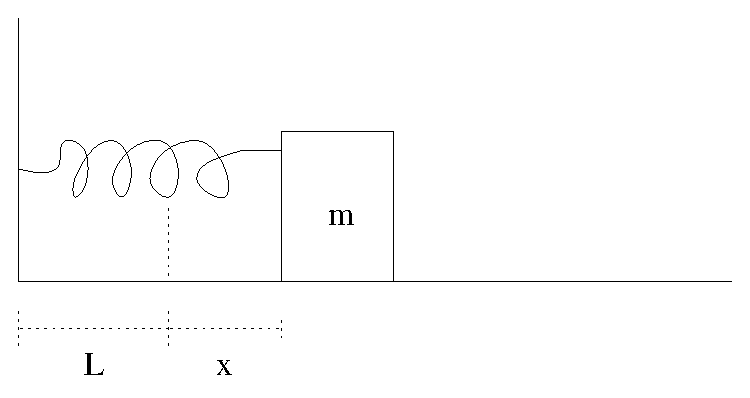
\psfig{file=figures/spring.eps,height=1.5in}}
      \caption{Hooke's Law spring.}
      \label{F:spring2}
\end{figure}


\subsection*{A Reduction to a First Order System}
\index{first order!reduction to}

There is a simple trick that reduces a single linear second order
differential equation to a system of two linear first order equations.
For example, consider the linear homogeneous ordinary differential
equation \Ref{eq:soex1}.  To reduce this second order equation to a first order
system, just set $y=\dot{x}$.  Then \Ref{eq:soex1} becomes
\[
\dot{y} + by + ax = 0.
\]
It follows that if $x(t)$ is a solution to \Ref{eq:soex1} and
$y(t)=\dot{x}(t)$, then $(x(t),y(t))$ is a solution to
\begin{equation}  \label{e:soex1sys}
\begin{array}{rcl}
\dot{x} & = & y \\
\dot{y} & = & -ax - by.
\end{array}
\end{equation}
We can rewrite \Ref{e:soex1sys} as
\[
\dot{X} = Q X.
\]
where
\begin{equation}  \label{e:coeffmatQ}
Q =  \mattwo{0}{1}{-a}{-b}.
\end{equation}
Note that if $(x(t),y(t))$ is a solution to \Ref{e:soex1sys}, then
$x(t)$ is a solution to \Ref{eq:soex1}.  Thus solving the single
second order linear equation is exactly the same as solving the
corresponding first order linear system.

\subsubsection*{The Initial Value Problem}
\index{initial value problem!for second order equations}

To solve the homogeneous system \Ref{e:soex1sys} we need to specify
two initial conditions $X(0)=(x(0),y(0))^t$.  It follows that to
solve the single second order equation we need to specify two initial
conditions $x(0)$ and $\dot{x}(0)$; that is, we need to specify
both initial position\index{initial position} and
initial velocity\index{initial velocity}.

\subsection*{The General Solution}

There are two ways in which we can solve
the second order homogeneous equation \Ref{eq:soex1}.  First,
we know how to solve the system \Ref{e:soex1sys} by finding the
eigenvalues and eigenvectors of the coefficient matrix $Q$ in
\Ref{e:coeffmatQ}.  Second, we know from the general theory of
planar systems that solutions will have the form $x(t)=e^{\lambda_0t}$
for some scalar $\lambda_0$.  We need only determine the values of
$\lambda_0$ for which we get solutions to \Ref{eq:soex1}.

We now discuss the second approach.  Suppose that $x(t)=e^{\lambda_0t}$
is a solution to \Ref{eq:soex1}.  Substituting this form of $x(t)$ in
\Ref{eq:soex1} yields the equation
\[
\left(\lambda_0^2 + b\lambda_0 + a\right)e^{\lambda_0t} = 0.
\]
So $x(t)=e^{\lambda_0t}$ is a solution to \Ref{eq:soex1} precisely
when $p_Q(\lambda_0)=0$, where
\begin{equation} \label{E:charQ}
p_Q(\lambda) = \lambda^2 + b\lambda + a
\end{equation}
is the characteristic polynomial of the matrix $Q$ in \Ref{e:coeffmatQ}.

Suppose that $\lambda_1$ and $\lambda_2$ are distinct real roots of $p_Q$.
Then the general solution\index{general solution} to \Ref{eq:soex1} is
\[
x(t) = \alpha_1e^{\lambda_1t} +  \alpha_2e^{\lambda_2t},
\]
where $\alpha_j\in\R$.

\subsubsection*{An Example with Distinct Real Eigenvalues}

For example, solve the initial value problem
\begin{equation} \label{e:ex12}
\ddot{x} + 3\dot{x} + 2x = 0
\end{equation}
with initial conditions $x(0)=0$ and $\dot{x}(0)=-2$.  The characteristic
polynomial is
\[
p_Q(\lambda) = \lambda^2 + 3\lambda + 2 = (\lambda+2)(\lambda+1),
\]
whose roots are $\lambda_1=-1$ and $\lambda_2=-2$.  So the general solution
to \Ref{e:ex12} is
\[
x(t) = \alpha_1e^{-t} + \alpha_2e^{-2t}
\]
To find the precise solution we need to solve
\[
\begin{array}{rclcl}
x(0) & = & \alpha_1 + \alpha_2 & = & 0 \\
\dot{x}(0) & = & -\alpha_1 - 2\alpha_2 & = & -2
\end{array}
\]
So $\alpha_1 = -2$, $\alpha_2=2$, and the solution to the initial value problem
for \Ref{e:ex12} is
\[
x(t) = -2e^{-t} + 2e^{-2t}
\]

\subsubsection*{An Example with Complex Conjugate Eigenvalues}

Consider the differential equation
\begin{equation} \label{E:ex13}
\ddot{x} -2\dot{x} + 5x = 0.
\end{equation}
The roots of the characteristic polynomial associated to \Ref{E:ex13} are
$\lambda_1=1+2i$ and $\lambda_2=1-2i$.  It follows from the discussion in
the previous section that the general solution to \Ref{E:ex13} is
\[
x(t) = \RE\left(\alpha_1 e^{\lambda_1 t} + \alpha_2 e^{\lambda_2t}\right)
\]
where $\alpha_1$ and $\alpha_2$ are complex scalars.  Indeed, we can rewrite
this solution in real form (using Euler's formula) as
\[
x(t) = e^t\left(\beta_1\cos(2t) + \beta_2\sin(2t)\right),
\]
for real scalars $\beta_1$ and $\beta_2$.

In general, if the roots of the characteristic polynomial are
$\sigma\pm i\tau$, then the general solution to the differential equation is:
\[
x(t) = e^{\sigma t}\left(\beta_1\cos(\tau t) + \beta_2\sin(\tau t)\right).
\]

\subsubsection*{An Example with Multiple Eigenvalues}

Note that the coefficient matrix $Q$ of the associated first order system
in \Ref{e:coeffmatQ} is never a multiple of $I_2$.  It follows from the
previous section
that when the roots of the characteristic polynomial are real and equal,
the general solution has the form
\[
x(t) = \alpha_1 e^{\lambda_1t} + \alpha_2te^{\lambda_2t}.
\]

\subsubsection*{Summary}

It follows from this discussion that solutions to second order
homogeneous linear equations are either a linear combination of two
exponentials (real unequal eigenvalues), $\alpha+\beta t$ times one
exponential (real equal eigenvalues), or a time periodic function times
an exponential (complex eigenvalues).

In particular, if the real part
of the complex eigenvalues is zero, then the solution is time periodic.
The frequency of this periodic solution is often called the {\em internal
frequency}\index{frequency!internal}, a point
that is made more clearly in the next example.


\subsection*{Solving the Spring Equation}

Consider the equation for the frictionless spring without
external forcing.  From \Ref{e:springeq} we get  \index{spring equation}
\index{spring!undamped}
\begin{equation} \label{ex:uspring}
m\ddot{x} + \kappa x = 0.
\end{equation}
where $\kappa>0$.  The roots are $\lambda_1=\sqrt{\frac{\kappa}{m}}i$
and $\lambda_2=-\sqrt{\frac{\kappa}{m}}i$.  So the general solution is
\[
x(t) = \alpha\cos(\tau t) + \beta\sin(\tau t),
\]
where $\tau=\sqrt{\frac{\kappa}{m}}$.  Under these assumptions the
motion of the spring is time periodic with period $\frac{2\pi}{\tau}$
or internal frequency $\frac{\tau}{2\pi}$.  In particular, the solution
satisfying initial conditions $x(0)=1$ and $\dot{x}(0)=0$ (the spring is
extended one unit in distance and released with no initial velocity) is
\[
x(t) = \cos(\tau t).
\]
The graph of this function when $\tau=1$ is given on the
left in Figure~\ref{F:springp}.
\begin{figure}[htb]
           \centerline{%
           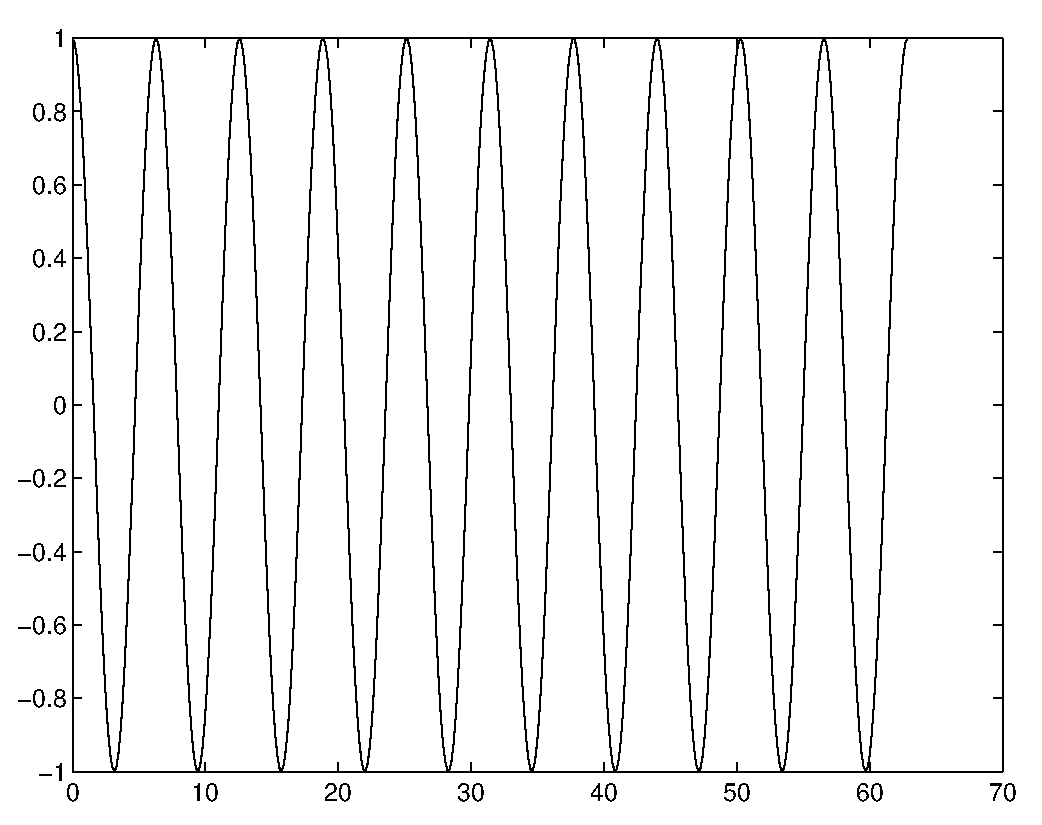
\psfig{file=figures/springp.eps,width=3.0in}
           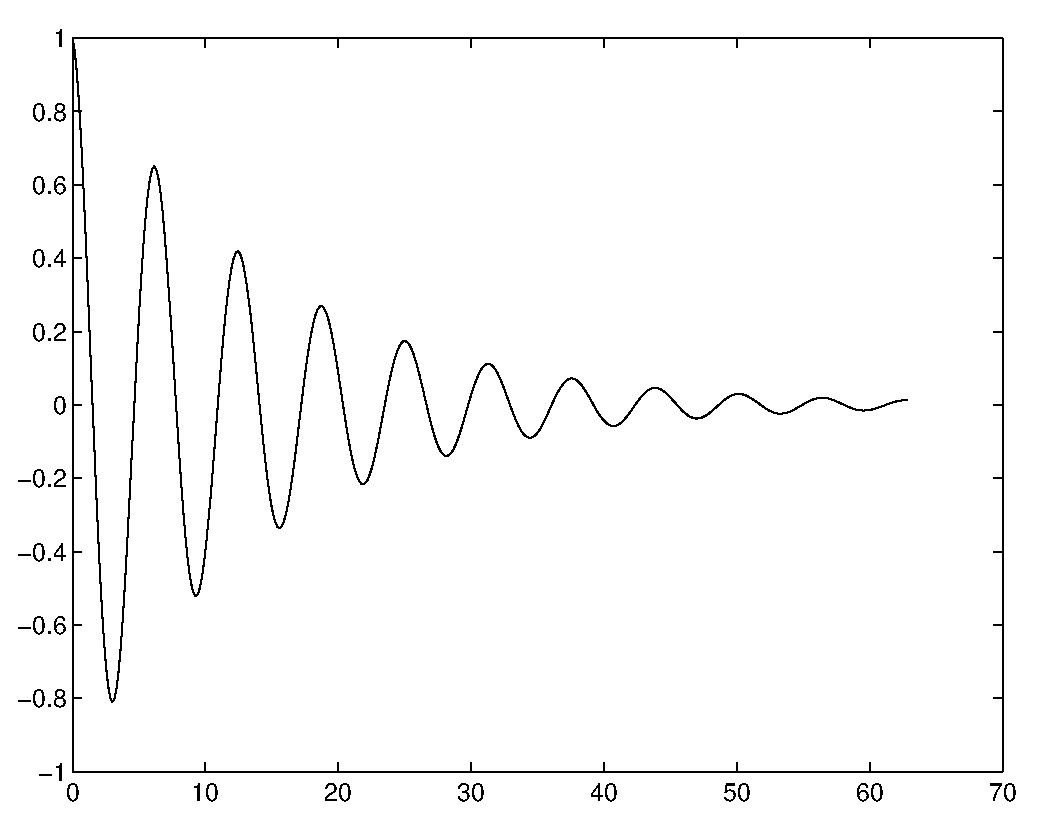
\psfig{file=figures/springpd.eps,width=3.0in}}
           \caption{(Left) Graph of solution to undamped spring
	equation with initial conditions $x(0)=1$ and $\dot{x}(0)=0$.
	(Right) Graph of solution to damped spring equation with the
	same initial conditions.}
           \label{F:springp}
\end{figure}

If a small amount of friction is added, then the spring equation is
\index{spring!damped}
\[
m\ddot{x} + \mu \dot{x} +\kappa x = 0
\]
where $\mu>0$ is small.  Since the eigenvalues of the characteristic
polynomial are $\lambda=\sigma\pm i\tau$ where
\[
\sigma = -\frac{\mu}{2m} < 0 \AND \tau =\sqrt{\frac{\kappa}{m}
-\left(\frac{\mu}{2m}\right)^2},
\]
the general solution is
\[
x(t) = e^{\sigma t}(\alpha\cos(\tau t) + \beta\sin(\tau t)).
\]
Since $\sigma<0$, these solutions oscillate but damp down to zero.  In
particular, the solution satisfying initial conditions $x(0)=1$ and
$\dot{x}(0)=0$ is
\[
x(t) = e^{-\mu t/2m}
\left(\cos(\tau t)-\frac{\mu}{2m\tau}\sin(\tau t)\right).
\]
The graph of this solution when $\tau=1$ and $\frac{\mu}{2m}=0.07$ is
given in Figure~\ref{F:springp} (right).  Compare the solutions for the
undamped and damped springs.

\EXER

\TEXER

\begin{exercise} \label{c6.7.1}
By direct integration solve the differential equation \Ref{e:pointpart}
for a point particle moving only under the influence of gravity.  Find the
solution for a particle starting at a height of $10$ feet above ground with
an upward velocity of $20$ feet/sec.  At what time will the particle hit
the ground?  (Recall that acceleration due to gravity is $32$ feet/sec$^2$.)
\end{exercise}

\begin{exercise} \label{c6.7.2}
By direct integration solve the differential equation \Ref{e:pointpart}
for a point particle moving only under the influence of gravity.  Show
that the solution is
\[
x(t) = -\frac{1}{2}gt^2 + v_0t + x_0
\]
where $x_0$ is the initial position of the particle and $v_0$ is the initial
velocity.
\end{exercise}

\noindent  In Exercises~\ref{c6.6.hoa} -- \ref{c6.6.hoc} find the general
solution to the given differential equation.
\begin{exercise} \label{c6.6.hoa}
$\ddot{x} + 2\dot{x} - 3x = 0$.
\end{exercise}
\begin{exercise} \label{c6.6.hob}
$\ddot{x} - 6\dot{x} + 9x = 0$.
In addition, find the solution to this equation satisfying
initial values $x(1)=1$ and $\dot{x}(1)=0$.
\end{exercise}
\begin{exercise} \label{c6.6.hoc}
$\ddot{x} + 2\dot{x} + 2x = 0$.
\end{exercise}

\begin{exercise} \label{c6.7.3}
Prove that a nonzero solution to a second order linear differential equation
with constant coefficients cannot be identically equal to zero on a nonempty
interval.
\end{exercise}

\begin{exercise} \label{c6.7.4}
Let $r>0$ and $w>0$ be constants, and let $x(t)$ be a solution to the
differential equation
\[
\ddot{x} + r\dot{x} + wx = 0.
\]
Show that $\dps\lim_{t\to\infty} x(t) = 0$.
\end{exercise}

\noindent In Exercises~\ref{c6.6.tfa} -- \ref{c6.6.tfc}, let $x(t)$ be a
solution to the second order linear homogeneous differential equation
\Ref{eq:soex1}.  Determine whether the given statement is {\em true\/}
or {\em false}.
\begin{exercise} \label{c6.6.tfa}
If $x(t)$ is nonconstant and time periodic, then the
roots of the characteristic polynomial are purely imaginary.
\end{exercise}
\begin{exercise} \label{c6.6.tfb}
If $x(t)$ is constant in $t$, then one of the roots of
the characteristic polynomial is zero.
\end{exercise}
\begin{exercise} \label{c6.6.tfc}
If $x(t)$ is not bounded, then the roots of the characteristic
polynomial are equal.
\end{exercise}

\begin{exercise} \label{c3.5.5}
Consider the second order differential equation
\begin{equation}  \label{E:2ndorder}
\frac{d^2x}{dt^2} + a(x)\frac{dx}{dt} + b(x) = 0.
\end{equation}
Let $y(t)=\dot{x}(t)$ and show that \Ref{E:2ndorder} may be
rewritten as a first order coupled system in $x(t)$ and $y(t)$
as follows:
\begin{eqnarray*}
\dot{x} & = & y \\
\dot{y} & = & -b(x) - a(x) y.
\end{eqnarray*}
\end{exercise}


\CEXER

\begin{exercise} \label{c6.7.5}
Use {\sf pplane5} to compute solutions to the system corresponding to the
spring equations with small sliding friction.  Plot the time series (in $x$)
of the solution and observe the oscillating and damping of the solution.
\end{exercise}







\end{document}

\documentclass{ximera}

 

\usepackage{epsfig}

\graphicspath{
  {./}
  {figures/}
}

\usepackage{morewrites}
\makeatletter
\newcommand\subfile[1]{%
\renewcommand{\input}[1]{}%
\begingroup\skip@preamble\otherinput{#1}\endgroup\par\vspace{\topsep}
\let\input\otherinput}
\makeatother

\newcommand{\includeexercises}{\directlua{dofile("/home/jim/linearAlgebra/laode/exercises.lua")}}

%\newcounter{ccounter}
%\setcounter{ccounter}{1}
%\newcommand{\Chapter}[1]{\setcounter{chapter}{\arabic{ccounter}}\chapter{#1}\addtocounter{ccounter}{1}}

%\newcommand{\section}[1]{\section{#1}\setcounter{thm}{0}\setcounter{equation}{0}}

%\renewcommand{\theequation}{\arabic{chapter}.\arabic{section}.\arabic{equation}}
%\renewcommand{\thefigure}{\arabic{chapter}.\arabic{figure}}
%\renewcommand{\thetable}{\arabic{chapter}.\arabic{table}}

%\newcommand{\Sec}[2]{\section{#1}\markright{\arabic{ccounter}.\arabic{section}.#2}\setcounter{equation}{0}\setcounter{thm}{0}\setcounter{figure}{0}}

\newcommand{\Sec}[2]{\section{#1}}

\setcounter{secnumdepth}{2}
%\setcounter{secnumdepth}{1} 

%\newcounter{THM}
%\renewcommand{\theTHM}{\arabic{chapter}.\arabic{section}}

\newcommand{\trademark}{{R\!\!\!\!\!\bigcirc}}
%\newtheorem{exercise}{}

\newcommand{\dfield}{{\sf dfield9}}
\newcommand{\pplane}{{\sf pplane9}}

\newcommand{\EXER}{\section*{Exercises}}%\vspace*{0.2in}\hrule\small\setcounter{exercise}{0}}
\newcommand{\CEXER}{}%\vspace{0.08in}\begin{center}Computer Exercises\end{center}}
\newcommand{\TEXER}{} %\vspace{0.08in}\begin{center}Hand Exercises\end{center}}
\newcommand{\AEXER}{} %\vspace{0.08in}\begin{center}Hand Exercises\end{center}}

% BADBAD: \newcommand{\Bbb}{\bf}

\newcommand{\R}{\mbox{$\Bbb{R}$}}
\newcommand{\C}{\mbox{$\Bbb{C}$}}
\newcommand{\Z}{\mbox{$\Bbb{Z}$}}
\newcommand{\N}{\mbox{$\Bbb{N}$}}
\newcommand{\D}{\mbox{{\bf D}}}
\usepackage{amssymb}
%\newcommand{\qed}{\hfill\mbox{\raggedright$\square$} \vspace{1ex}}
%\newcommand{\proof}{\noindent {\bf Proof:} \hspace{0.1in}}

\newcommand{\setmin}{\;\mbox{--}\;}
\newcommand{\Matlab}{{M\small{AT\-LAB}} }
\newcommand{\Matlabp}{{M\small{AT\-LAB}}}
\newcommand{\computer}{\Matlab Instructions}
\newcommand{\half}{\mbox{$\frac{1}{2}$}}
\newcommand{\compose}{\raisebox{.15ex}{\mbox{{\scriptsize$\circ$}}}}
\newcommand{\AND}{\quad\mbox{and}\quad}
\newcommand{\vect}[2]{\left(\begin{array}{c} #1_1 \\ \vdots \\
 #1_{#2}\end{array}\right)}
\newcommand{\mattwo}[4]{\left(\begin{array}{rr} #1 & #2\\ #3
&#4\end{array}\right)}
\newcommand{\mattwoc}[4]{\left(\begin{array}{cc} #1 & #2\\ #3
&#4\end{array}\right)}
\newcommand{\vectwo}[2]{\left(\begin{array}{r} #1 \\ #2\end{array}\right)}
\newcommand{\vectwoc}[2]{\left(\begin{array}{c} #1 \\ #2\end{array}\right)}

\newcommand{\ignore}[1]{}


\newcommand{\inv}{^{-1}}
\newcommand{\CC}{{\cal C}}
\newcommand{\CCone}{\CC^1}
\newcommand{\Span}{{\rm span}}
\newcommand{\rank}{{\rm rank}}
\newcommand{\trace}{{\rm tr}}
\newcommand{\RE}{{\rm Re}}
\newcommand{\IM}{{\rm Im}}
\newcommand{\nulls}{{\rm null\;space}}

\newcommand{\dps}{\displaystyle}
\newcommand{\arraystart}{\renewcommand{\arraystretch}{1.8}}
\newcommand{\arrayfinish}{\renewcommand{\arraystretch}{1.2}}
\newcommand{\Start}[1]{\vspace{0.08in}\noindent {\bf Section~\ref{#1}}}
\newcommand{\exer}[1]{\noindent {\bf \ref{#1}}}
\newcommand{\ans}{}
\newcommand{\matthree}[9]{\left(\begin{array}{rrr} #1 & #2 & #3 \\ #4 & #5 & #6
\\ #7 & #8 & #9\end{array}\right)}
\newcommand{\cvectwo}[2]{\left(\begin{array}{c} #1 \\ #2\end{array}\right)}
\newcommand{\cmatthree}[9]{\left(\begin{array}{ccc} #1 & #2 & #3 \\ #4 & #5 &
#6 \\ #7 & #8 & #9\end{array}\right)}
\newcommand{\vecthree}[3]{\left(\begin{array}{r} #1 \\ #2 \\
#3\end{array}\right)}
\newcommand{\cvecthree}[3]{\left(\begin{array}{c} #1 \\ #2 \\
#3\end{array}\right)}
\newcommand{\cmattwo}[4]{\left(\begin{array}{cc} #1 & #2\\ #3
&#4\end{array}\right)}

\newcommand{\Matrix}[1]{\ensuremath{\left(\begin{array}{rrrrrrrrrrrrrrrrrr} #1 \end{array}\right)}}

\newcommand{\Matrixc}[1]{\ensuremath{\left(\begin{array}{cccccccccccc} #1 \end{array}\right)}}



\renewcommand{\labelenumi}{\theenumi)}
\newenvironment{enumeratea}%
{\begingroup
 \renewcommand{\theenumi}{\alph{enumi}}
 \renewcommand{\labelenumi}{(\theenumi)}
 \begin{enumerate}}
 {\end{enumerate}\endgroup}



\newcounter{help}
\renewcommand{\thehelp}{\thesection.\arabic{equation}}

%\newenvironment{equation*}%
%{\renewcommand\endequation{\eqno (\theequation)* $$}%
%   \begin{equation}}%
%   {\end{equation}\renewcommand\endequation{\eqno \@eqnnum
%$$\global\@ignoretrue}}

%\input{psfig.tex}

\author{Martin Golubitsky and Michael Dellnitz}

%\newenvironment{matlabEquation}%
%{\renewcommand\endequation{\eqno (\theequation*) $$}%
%   \begin{equation}}%
%   {\end{equation}\renewcommand\endequation{\eqno \@eqnnum
% $$\global\@ignoretrue}}

\newcommand{\soln}{\textbf{Solution:} }
\newcommand{\exercap}[1]{\centerline{Figure~\ref{#1}}}
\newcommand{\exercaptwo}[1]{\centerline{Figure~\ref{#1}a\hspace{2.1in}
Figure~\ref{#1}b}}
\newcommand{\exercapthree}[1]{\centerline{Figure~\ref{#1}a\hspace{1.2in}
Figure~\ref{#1}b\hspace{1.2in}Figure~\ref{#1}c}}
\newcommand{\para}{\hspace{0.4in}}

\renewenvironment{solution}{\suppress}{\endsuppress}

\ifxake
\newenvironment{matlabEquation}{\begin{equation}}{\end{equation}}
\else
\newenvironment{matlabEquation}%
{\let\oldtheequation\theequation\renewcommand{\theequation}{\oldtheequation*}\begin{equation}}%
  {\end{equation}\let\theequation\oldtheequation}
\fi

\makeatother


\title{c7.tex}

\begin{document}
\begin{abstract}
BADBAD
\end{abstract}
\maketitle

\chapter{Qualitative Theory of Planar ODEs}
\label{Chap:PlanarQ}

\normalsize

Chapter~\ref{Chap:Planar} discussed three methods that are used to solve
planar systems of linear, constant coefficient, ordinary differential
equations.  The last method is based on similarity and the explicit
computation of the matrix exponential for certain normal form matrices.
This method depends crucially on the classification of $2\times 2$ matrices
up to similarity given in Chapter~\ref{Chap:Planar}, 
Theorem~\ref{T:putinform}.

In this chapter we explore qualitative features of phase portraits for planar 
linear systems of differential equations using similarity.  We find that the 
qualitative theory is completely determined by the eigenvalues and 
eigenvectors of the coefficient matrix --- which is not surprising given
that we can classify matrices up to similarity by just knowing their
eigenvalues and eigenvectors.  The set of planar phase portraits divides 
systems of linear differential equations into two camps: {\em hyperbolic\/} 
and {\em nonhyperbolic\/}.  The hyperbolic systems consist of {\em saddles\/},
{\em sinks\/} and {\em sources\/}, while the nonzero nonhyperbolic systems 
consist of {\em centers\/}, {\em saddle nodes\/}, and {\em shears\/}.


\section{Sinks, Saddles, and Sources} \label{S:6.7}

The qualitative theory of autonomous differential equations begins with
the observation that many important properties of solutions to constant
coefficient systems of differential equations
\begin{equation} \label{e:C2}
\frac{dX}{dt}=CX
\end{equation}
are unchanged by similarity.

Begin by noting that the origin is always an equilibrium for \Ref{e:C2}
and suppose that $C$ is a $2\times 2$ matrix.  The origin for \Ref{e:C2}
is called a {\em sink\/}\index{sink} if the eigenvalues of $C$ both have
negative real
part and a {\em source\/}\index{source} if the eigenvalues both have
positive real part.
When $C$ has one eigenvalue of each sign, the origin is called a
{\em saddle}\index{saddle}.

Now suppose that $B$ is a $2\times 2$ matrix that is similar to $C$.
Lemma~\ref{L:simdettr} of Chapter~\ref{Chap:Planar} states that $B$ and
$C$ have the same eigenvalues.  It follows that if the origin is a saddle
for \Ref{e:C2}, then it is a saddle for $\dot{X}=BX$.  Similar statements
hold for sinks and sources.

\subsection*{Asymptotic Stability}

We now discuss asymptotic stability of the origin in linear systems.
Recall from our discussion in Section~\ref{sec:UncoupledLS} 
that the origin is {\em asymptotically stable\/} \index{stability!asymptotic}
if every trajectory $X(t)$ beginning at an initial condition near the
origin stays near $0$ for all positive $t$, and
\[
\lim_{t\to\infty}X(t) = 0.
\]
Recall also from Lemma~\ref{L:simsoln} of Chapter~\ref{Chap:Planar} that
if $B=P\inv CP$, then $P\inv X(t)$ is a solution to $\dot{X}=BX$ whenever
$X(t)$ is a solution to \Ref{e:C2}.  Since $P\inv$ is a matrix of constants
that do not depend on $t$, it follows that
\[
\lim_{t\to\infty}X(t) = 0 \Longleftrightarrow \lim_{t\to\infty}P\inv X(t) = 0.
\]
So the origin is asymptotically stable for $\dot{X}=BX$ if and only if it is
asymptotically stable for \Ref{e:C2}.  With this observation in hand, we
prove that sinks are stable.

\begin{thm}  \label{C:asympstlin}
If the eigenvalues of $C$ have negative real part, then the origin
is an asymptotically stable equilibrium\index{equilibrium} for \Ref{e:C2}.
If one of the
eigenvalues of $C$ has positive real part, then the origin is unstable.
\end{thm}

\proof  This proof is based on the closed form of solutions given in
Section~\ref{S:6.5}.   The remark preceding this theorem states that we
need only prove this theorem for differential equations up to similarity.

\noindent (a) \quad If the eigenvalues $\lambda_1$ and $\lambda_2$ are real
and there are two independent eigenvectors, then Chapter~\ref{Chap:Planar},
Theorem~\ref{T:putinform} states that the matrix $C$ is similar to the
diagonal matrix
\[
B = \mattwoc{\lambda_1}{0}{0}{\lambda_2}.
\]
The general solution to the differential equation $\dot{X}=BX$ is
\[
x_1(t) = \alpha_1e^{\lambda_1 t} \AND x_2(t) = \alpha_2e^{\lambda_2 t}.
\]
Since
\[
\lim_{t\to\infty}e^{\lambda_1 t} = 0  = \lim_{t\to\infty}e^{\lambda_2 t},
\]
when $\lambda_1$ and $\lambda_2$ are negative, it follows that
\[
\lim_{t\to\infty} X(t) = 0
\]
for all solutions $X(t)$, and the origin is asymptotically stable.  Note that
if one of the eigenvalues, say $\lambda_1$, is positive then $x_1(t)$ will
undergo exponential growth and the origin is unstable.

\noindent (b) \quad If the eigenvalues of $C$ are the complex conjugates
$\sigma\pm i\tau$ where $\tau\neq 0$, then Chapter~\ref{Chap:Planar},
Theorem~\ref{T:putinform} states that after a similarity transformation
\Ref{e:C2} has the form
\[
\dot{X} = \mattwo{\sigma}{-\tau}{\tau}{\sigma}X,
\]
and solutions for this equation have the form \Ref{e:exp0ev} of
Chapter~\ref{Chap:Planar}, that is,
\[
X(t) = e^{\sigma t}
\mattwo{\cos(\tau t)}{-\sin(\tau t)}{\sin(\tau t)}{\cos(\tau t)}X_0
= e^{\sigma t}R_{\tau t}X_0,
\]
where $R_{\tau t}$ is a rotation matrix\index{rotation!matrix}
(recall \Ref{e:rotmat} of
Chapter~\ref{chap:matrices}).  It follows that as time evolves
the vector $X_0$ is rotated about the origin and then expanded or contracted
by the factor $e^{\sigma t}$.  So when $\sigma<0$, $\lim_{t\to\infty} X(t)=0$
for all solutions $X(t)$.  Hence the origin is asymptotically stable.  Note
that when $\sigma>0$ solutions spiral away from the origin.

\noindent (c) \quad If the eigenvalues are both equal to $\lambda_1$
and if there is only one independent eigenvector, then
Chapter~\ref{Chap:Planar}, Theorem~\ref{T:putinform} states that after a
similarity transformation \Ref{e:C2} has the form
\[
\dot{X} = \mattwo{\lambda_1}{1}{0}{\lambda_1}X,
\]
whose solutions are
\[
X(t) = e^{t\lambda}\mattwoc{1}{t}{0}{1} X_0
\]
using \Ref{e:expshear} of Chapter~\ref{Chap:Planar}. Note that the functions
$e^{\lambda_1 t} \AND te^{\lambda_1 t}$ both have limits equal to zero as
$t\to\infty$.  In the second case, use l'H\^{o}spital's rule and the
assumption that $-\lambda_1>0$ to compute
\[
\lim_{t\to\infty} \frac{t}{e^{-\lambda_1 t}} =
  -\lim_{t\to\infty} \frac{1}{\lambda_1 e^{-\lambda_1 t}} = 0.
\]
Hence $\lim_{t\to\infty} X(t) =0$ for all solutions $X(t)$ and the origin
is asymptotically stable.  Note that initially $||X(t)||$ can grow since
$t$ is increasing.  But eventually exponential decay wins out and solutions
limit on the origin.   Note that solutions grow exponentially when
$\lambda_1>0$.  \qed

It is instructive to note how the time series $x_1(t)$ damps down to the
origin in the three cases listed in Theorem~\ref{C:asympstlin}.
In Figure~\ref{F:oscil} we present the time series for the three
coefficient matrices:
\[
C_1 = \mattwo{-2}{0}{0}{-1} \qquad
C_2 = \mattwo{-1}{-55}{55}{-1} \qquad
C_3 = \mattwo{-2}{1}{0}{-2}.
\]
In this figure, we can see the exponential decay to zero associated with the
unequal real eigenvalues of $C_1$; the damped oscillation associated with the
complex eigenvalues of $C_2$; and the initial growth of the time series due
to the $te^{-2t}$ term followed by exponential decay to zero in the equal
eigenvalue $C_3$ example.

\begin{figure}[htb]
           \centerline{%
           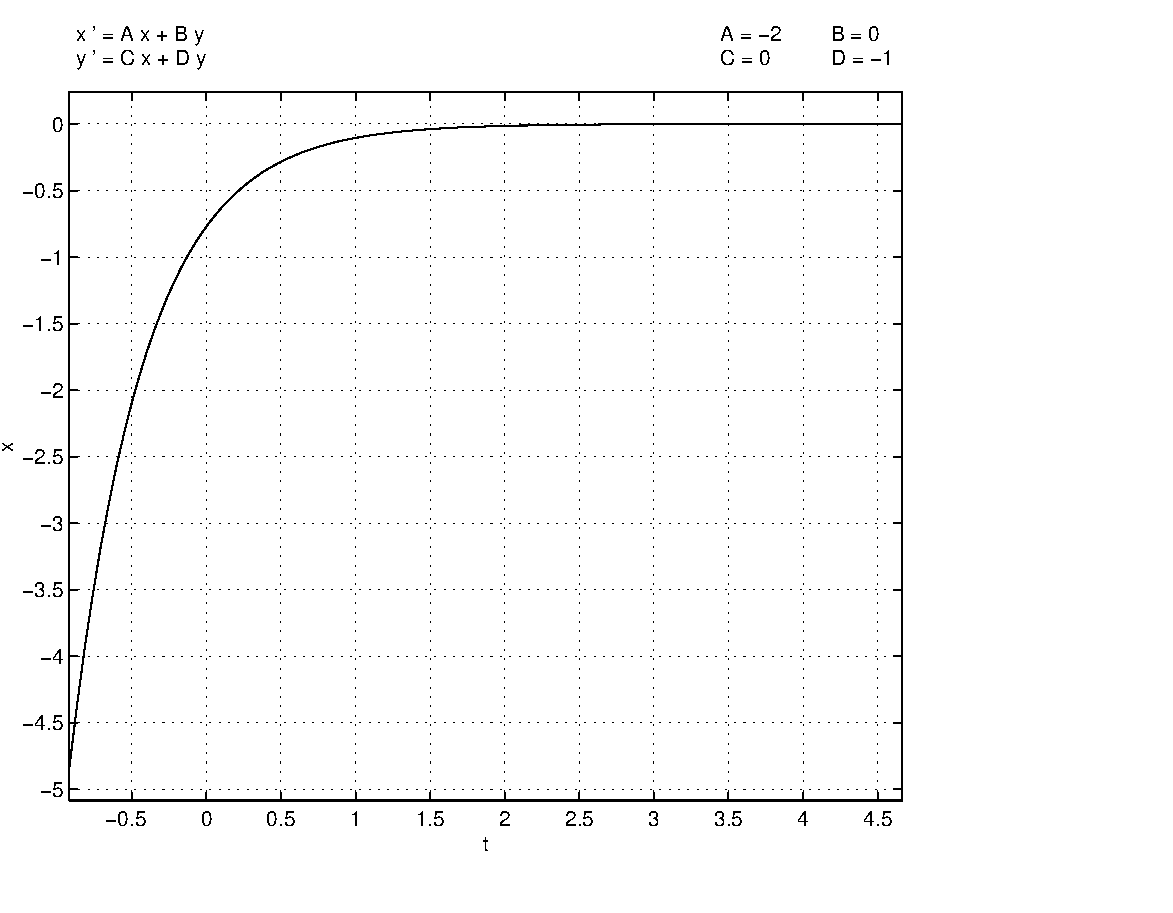
\psfig{file=figures/expdamp.eps,width=2.2in}
	   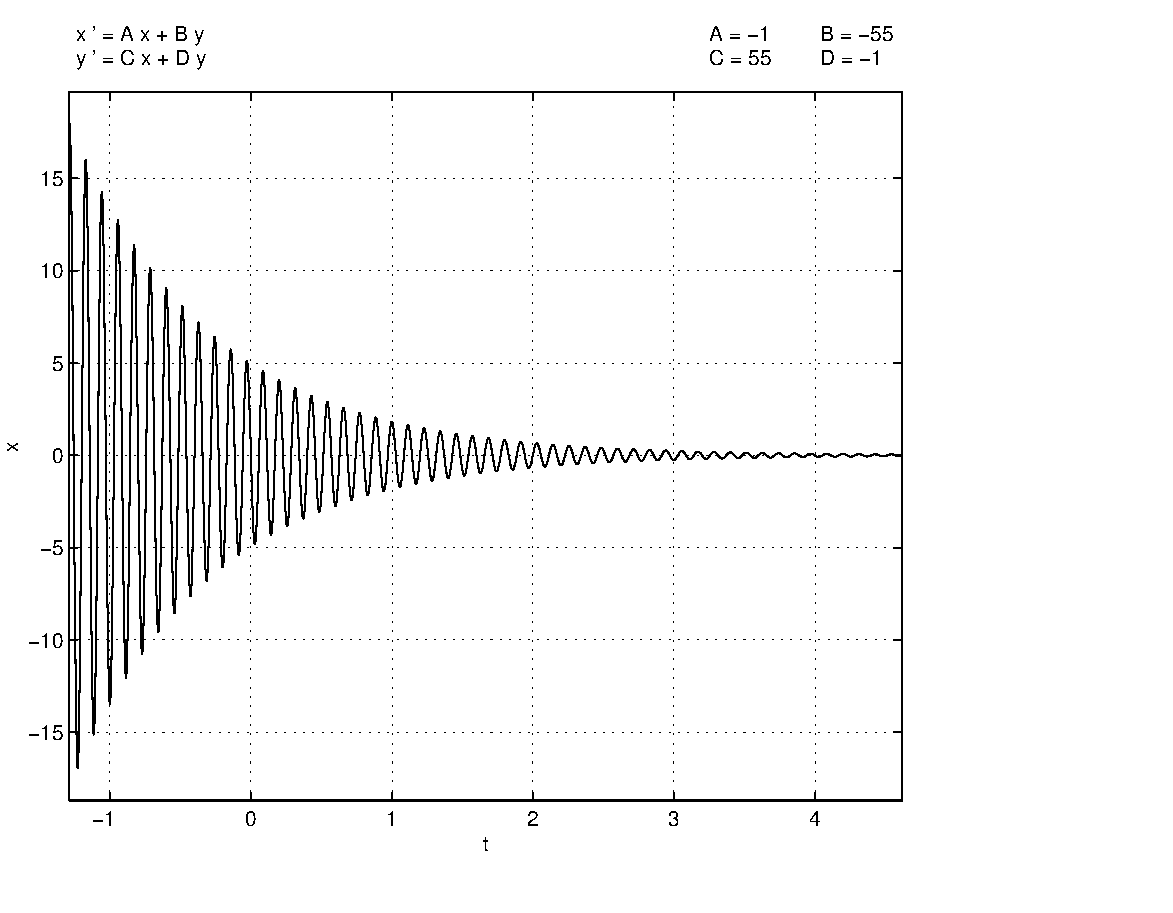
\psfig{file=figures/oscil.eps,width=2.2in}
	   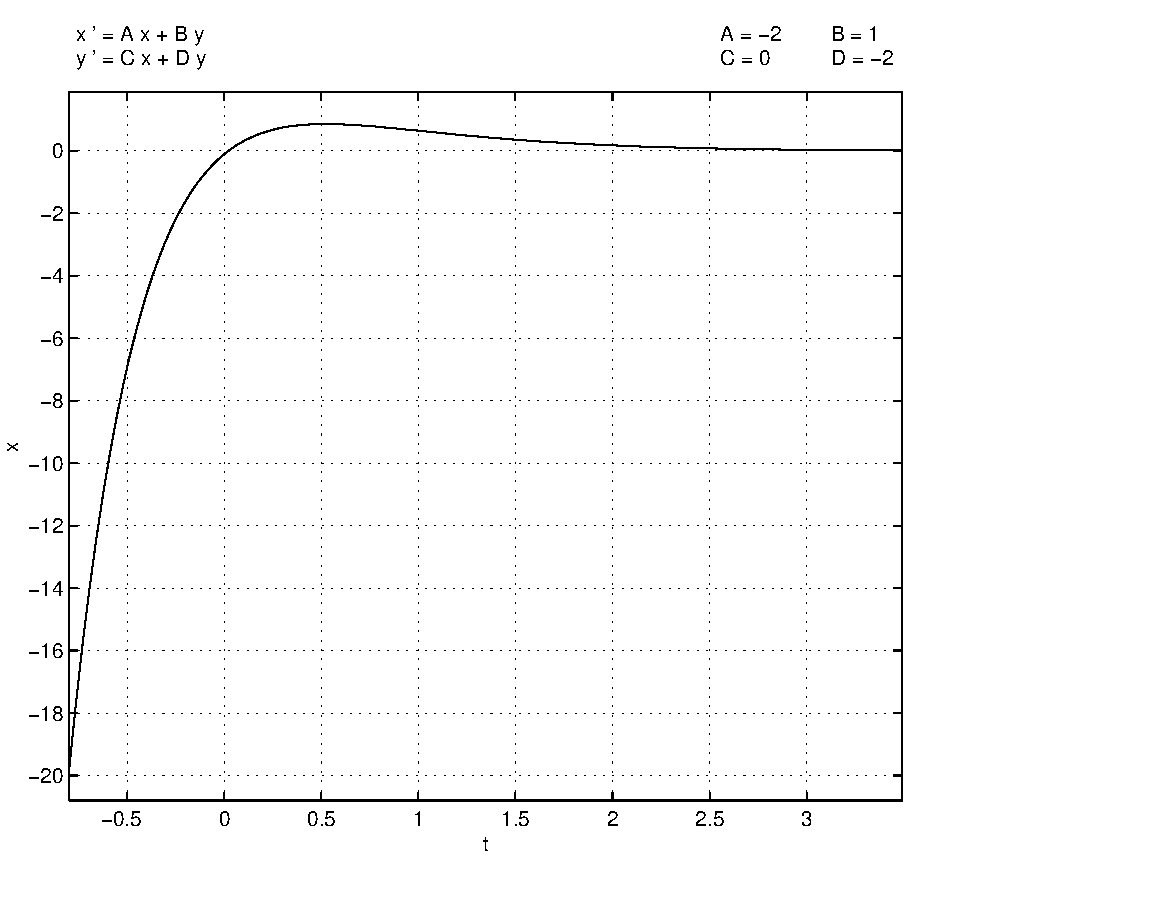
\psfig{file=figures/grdecay.eps,width=2.2in}}
           \caption{Time series for different sinks.}
           \label{F:oscil}
\end{figure}


\subsubsection*{Linear Stability}

Saddles, sinks, and sources are distinguished by the stability of the
origin.  In Theorem~\ref{C:asympstlin} we showed that the origin is
asymptotically stable if the eigenvalues have negative real part, that is,
if the origin is a sink.  There is another term that is commonly used and
is synonymous with sink.
\begin{Def} \label{D:linstablin}
The origin is a {\em linearly stable\/} equilibrium of \Ref{e:C2} if the
eigenvalues of $C$ have negative real part.
\end{Def}\index{stability!linear}
So Theorem~\ref{C:asympstlin} may be restated as: linear stability
implies asymptotic stability of the origin.

\subsubsection*{Sources Versus Sinks}

The explicit form of solutions to planar linear systems shows that solutions
with initial conditions near the origin grow exponentially in forward time
when the origin of \Ref{e:C2} is a source.  We can prove this point
geometrically, as follows.

The phase planes of sources and sinks are almost the same; they have the
same trajectories but the arrows are reversed.  To verify this point, note
that
\begin{equation}  \label{e:C3}
\dot{X}=-CX
\end{equation}
is a sink when \Ref{e:C2} is a source; observe that the trajectories of
solutions of \Ref{e:C2} are the same as those of \Ref{e:C3} --- just with
time running backwards.  For let $X(t)$ be a solution to \Ref{e:C2}; then
$X(-t)$ is a solution to \Ref{e:C3}.   See Figure~\ref{F:SS} for plots of
$\dot{X}=BX$ and $\dot{X}=-BX$ where
\begin{equation}  \label{E:SS}
B = \mattwo{-1}{-5}{5}{-1}.
\end{equation}

So when we draw schematic phase portraits\index{phase!portrait}
for sinks\index{phase!portrait!for a sink}, we automatically know
how to draw schematic phase portraits for
sources\index{phase!portrait!for a source}.  The trajectories are
the same --- but the arrows point in the opposite direction.

\begin{figure}[htb]
           \centerline{%
	   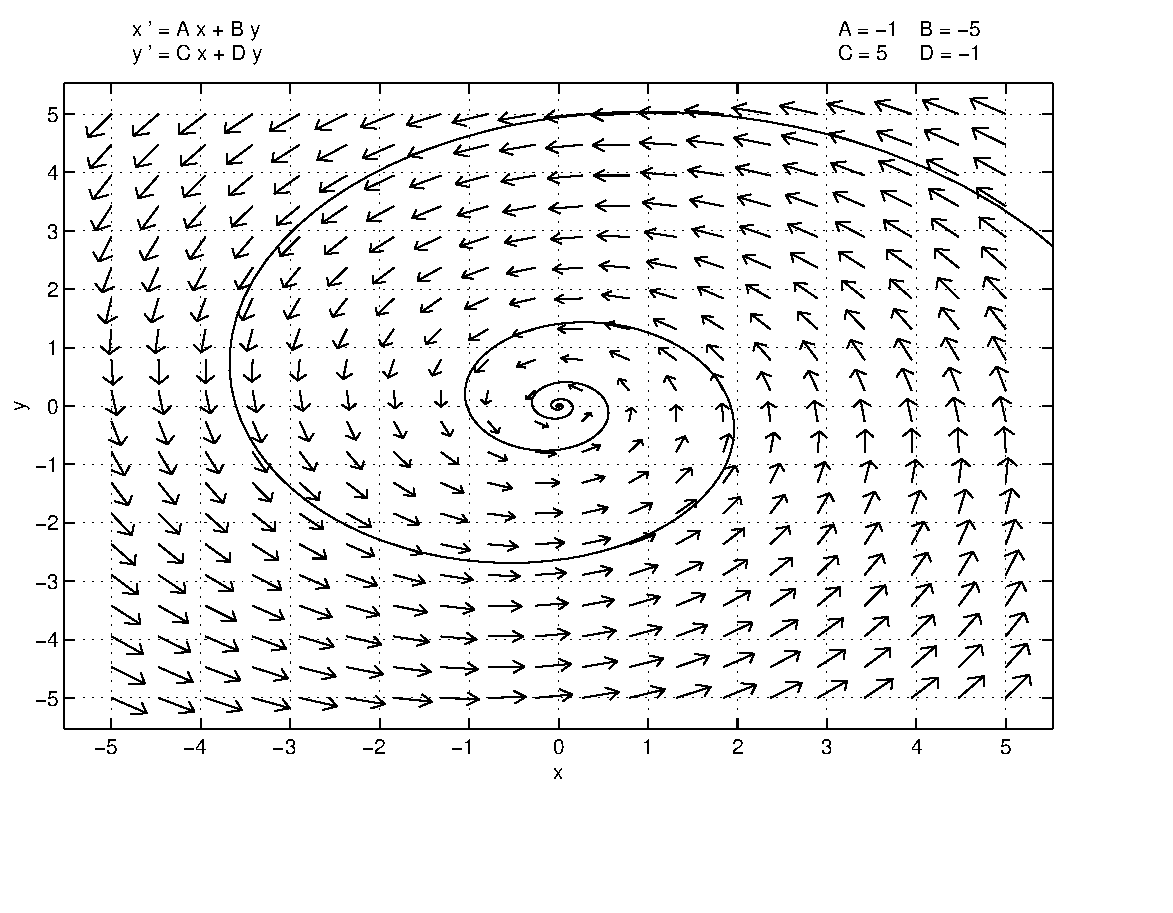
\psfig{file=figures/asink.eps,width=3.2in}
           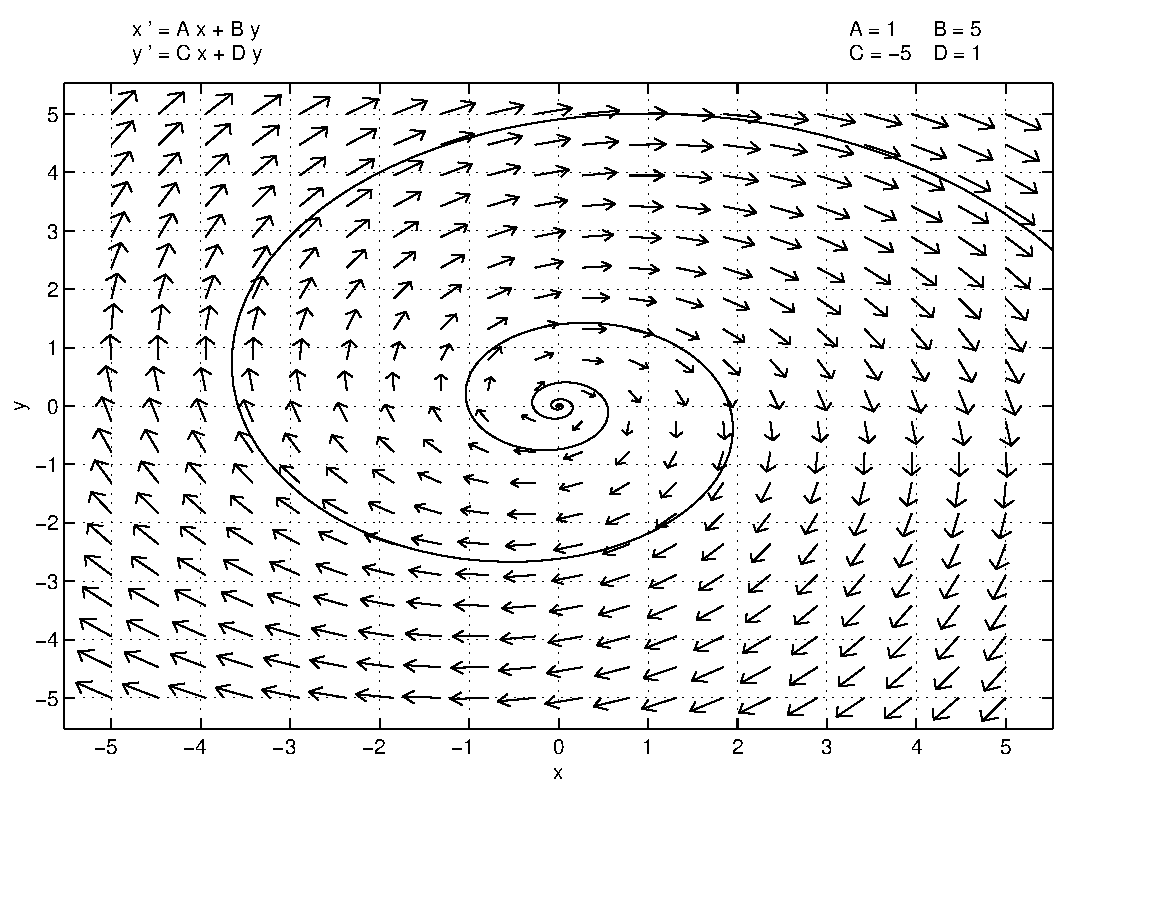
\psfig{file=figures/asource.eps,width=3.2in}}
           \caption{(Left) Sink $\dot{X}=BX$ where $B$ is given in
\protect{\Ref{E:SS}}.  (Right) Source $\dot{X}=-BX$.}
           \label{F:SS}
\end{figure}


\subsection*{Phase Portraits for Saddles}
\index{phase!portrait!for a saddle}

Next we discuss the phase portraits of linear saddles.  Using
{\sf pplane5}\index{\computer!pplane5}, draw the phase portrait
of the saddle
\begin{equation}  \label{e:saddlet}
\begin{array}{rcl}
\dot{x} & = & 2x+y\\
\dot{y} & = & -x-3y,
\end{array}
\end{equation}
as in Figure~\ref{F:linsaddle}.  The important feature of saddles
is that there are special trajectories (the eigendirections) that
limit on the origin in either forward or backward time.

\begin{figure}[htb]
           \centerline{%
	   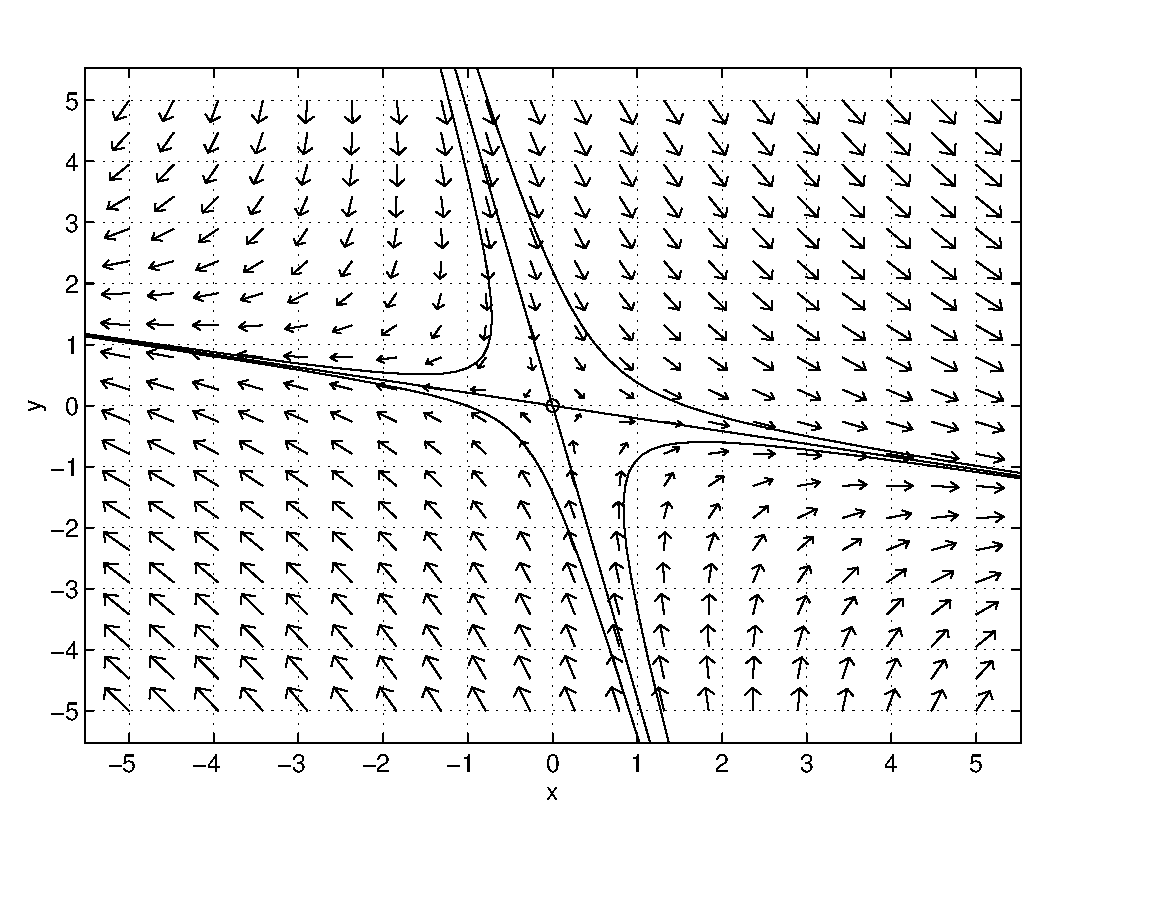
\psfig{file=figures/linpnb.eps,width=3.5in}
           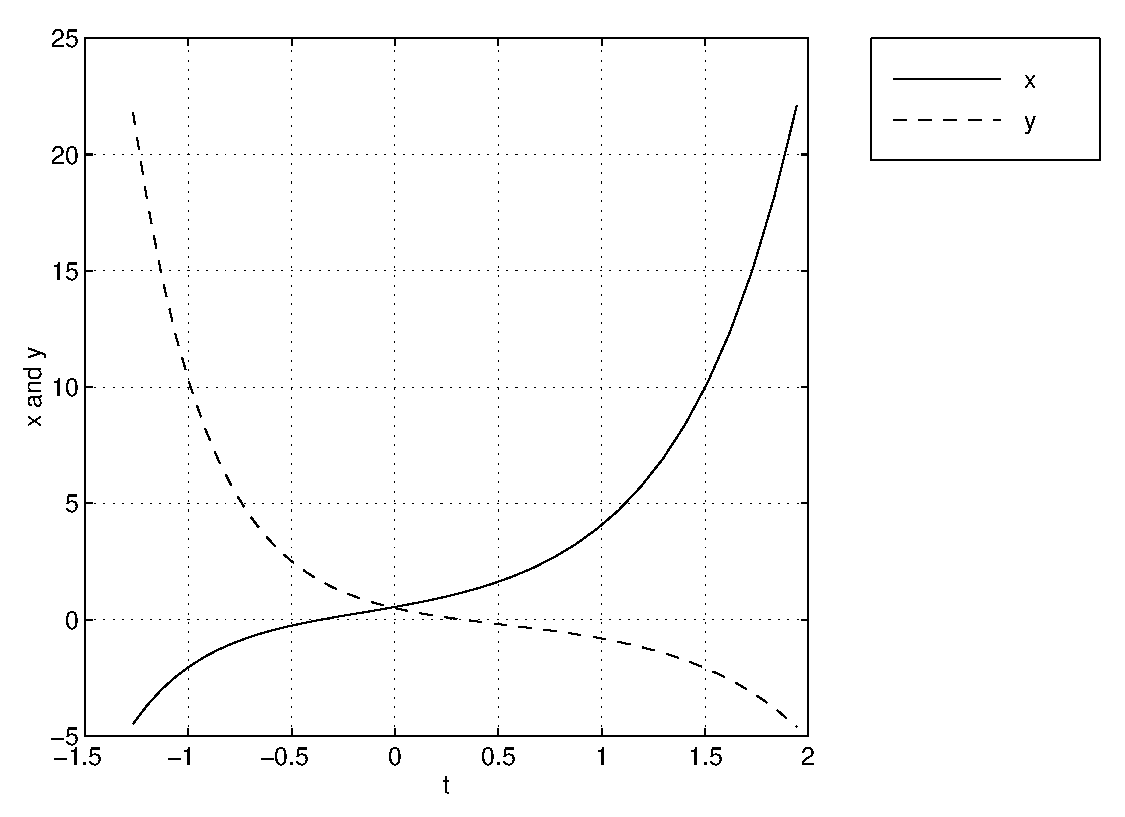
\psfig{file=figures/linpnts.eps,width=3.5in}}
           \caption{(Left) Saddle phase portrait.
	(Right) First quadrant solution time series.}
           \label{F:linsaddle}
\end{figure}

\begin{Def} \label{D:stablemfld}
The {\em stable manifold\/} or {\em stable orbit\/} of a saddle consists of
those trajectories that limit on the origin in forward time; the
{\em unstable manifold\/} or {\em unstable orbit\/} of a saddle consists of
those trajectories that limit on the origin in backward time.
\end{Def}
\index{stable!manifold} \index{unstable!manifold}
\index{stable!orbit} \index{unstable!orbit}

Let $\lambda_1<0$ and $\lambda_2>0$ be the eigenvalues of a saddle with
associated eigenvectors $v_1$ and $v_2$.  The stable orbits are given by the
solutions $X(t) = \pm e^{\lambda_1 t}v_1$ and the unstable orbits are given
by the solutions $X(t) = \pm e^{\lambda_2 t}v_2$.

\subsubsection*{Stable and Unstable Orbits using {\sf pplane5}}

The program {\sf pplane5} is programmed to draw the stable and unstable
orbits of a saddle on command. Although the principal use of this
feature is seen when analyzing nonlinear systems, it is useful to
introduce this feature here.  As an example, load the linear system
\Ref{e:saddlet} into {\sf pplane5} and click on {\sf Proceed}.  Now
pull down the {\sf PPLANE5 Options} menu and click on {\sf Find an
equilibrium}.  Click the cross hairs in the {\sf PPLANE5 Display}
window on a point near the origin; {\sf pplane5} responds by
opening a new window --- the {\sf PPLANE5 Equilibrium point data}
window --- and by putting a small yellow circle about the
origin.  The circle indicates that the numerical algorithm
programmed into {\sf pplane5} has detected an equilibrium near
the chosen point. A new window opens and displays the message
{\sf There is a saddle point at} $(0,0)$.  This window also displays the
coefficient matrix (called the Jacobian for reasons that will be discussed
in Section~\ref{S:linearization}) at the equilibrium and its eigenvalues
and eigenvectors.  This process numerically verifies that the origin
is a saddle (a fact that could have been verified in a more
straightforward way).

Now pull down the {\sf PPLANE5 Options} menu again and click on
{\sf Plot stable and unstable orbits}.  Next click on the mouse
when the cross hairs are within the yellow circle and {\sf
pplane5} responds by drawing the stable and unstable orbits.
The result is shown in Figure~\ref{F:linsaddle}(left).
On this figure we have also plotted one trajectory
from each quadrant; thus obtaining the phase portrait of a saddle.
On the right of Figure~\ref{F:linsaddle} we have plotted a
time series of the first quadrant solution.  Note how the $x$
time series increases exponentially to $+\infty$ in forward time and 
the $y$ time series decreases in forward time while going exponentially 
towards $-\infty$.  The two time series together
give the trajectory $(x(t),y(t))$ that in forward time is asymptotic
to the line given by the unstable eigendirection.



\EXER

\TEXER


\noindent In Exercises~\ref{E:stabmata} -- \ref{E:stabmatc} determine
whether or not the equilibrium at the origin in the system of differential
equations $\dot{X}=CX$ is asymptotically stable.
\begin{exercise} \label{E:stabmata}
$C=\mattwo{1}{2}{4}{1}$.
\end{exercise}
\begin{exercise} \label{E:stabmatb}
$C=\mattwo{-1}{2}{-4}{-1}$.
\end{exercise}
\begin{exercise} \label{E:stabmatc}
$C=\mattwo{2}{1}{1}{-5}$.
\end{exercise}

\noindent In Exercises~\ref{E:sisasoa} -- \ref{E:sisasof} determine
whether the equilibrium at the origin in the system of differential
equations $\dot{X}=CX$ is a sink, a saddle or a source.
\begin{exercise} \label{E:sisasoa}
$C=\mattwo{-2}{2}{0}{-1}$.
\end{exercise}
\begin{exercise} \label{E:sisasob}
$C=\mattwo{3}{5}{0}{-2}$.
\end{exercise}
\begin{exercise} \label{E:sisasoc}
$C=\mattwo{4}{2}{-1}{2}$.
\end{exercise}
\begin{exercise} \label{E:sisasod}
$C=\mattwo{8}{0}{-5}{3}$.
\end{exercise}
\begin{exercise} \label{E:sisasoe}
$C=\mattwo{9}{-11}{-11}{9}$.
\end{exercise}
\begin{exercise} \label{E:sisasof}
$C=\mattwo{1}{-8}{2}{1}$.
\end{exercise}

\CEXER

\noindent In Exercises~\ref{E:sssa} -- \ref{E:sssd} use {\sf pplane5} to
determine whether the origin is a saddle, sink, or source in $\dot{X}=CX$
for the given matrix $C$.
\begin{exercise} \label{E:sssa}
$C=\mattwoc{10}{-2.7}{4.32}{1.6}$.
\end{exercise}
\begin{exercise} \label{E:sssb}
$C=\mattwoc{-10}{-2.7}{4.32}{1.6}$.
\end{exercise}
\begin{exercise} \label{E:sssc}
$C=\mattwoc{-1}{2}{4.76}{1.5}$.
\end{exercise}
\begin{exercise} \label{E:sssd}
$C=\mattwo{-2}{-2}{4}{1}$.
\end{exercise}


\noindent In Exercises~\ref{E:sima} -- \ref{E:simb} the given matrices $B$
and $C$ are similar.  Observe that the phase portraits of the systems
$\dot{X}=BX$ and $\dot{X}=CX$ are qualitatively the same in two steps.
\begin{itemize}
\item[(a)]  Use \Matlab to find the $2\times 2$ matrix $P$ such that
$B=P\inv CP$.  Use {\tt map} to understand how the matrix $P$ moves points 
in the plane.
\item[(b)]  Use {\sf pplane5} to observe that $P$ moves solutions of
$\dot{X}=BX$ to the solution of $\dot{X}=CX$.  Write a sentence or two describing your results.
\end{itemize}
\begin{exercise} \label{E:sima}
$C = \mattwo{2}{3}{-1}{-3} \AND B = \frac{1}{2}\mattwo{1}{-1}{-9}{-3}$.
\end{exercise}
\begin{exercise} \label{E:simb}
$C = \mattwo{-1}{5}{-5}{-1} \AND B = \mattwo{-1}{0.5}{-50}{-1}$.
\end{exercise}






\section{Phase Portraits of Sinks}  \label{S:PlanarSystems}

In this section we describe phase portraits and time series of
solutions for different kinds of sinks. Sinks have coefficient
matrices whose eigenvalues have negative real part.  There are
four types of sinks\index{sink}:
\begin{enumerate}
\item {\em spiral sink\/} --- complex eigenvalues\index{sink},
\item {\em nodal sink\/} --- real unequal eigenvalues\index{nodal sink},
\item {\em focus sink\/} --- real equal eigenvalues; two independent
eigenvectors\index{focus!sink}, and
\item {\em improper nodal sink\/} --- real equal eigenvalues; one independent
eigenvector\index{nodal sink!improper}.
\end{enumerate}
In the previous section we showed that all solutions of sinks tend toward
the origin in forward time.  The way in which these solutions approach the
origin distinguishes the different sink types.  See Figure~\ref{F:oscil}.
We discuss each type of sink in turn, noting that
spiral and nodal sinks are the ones that are most likely to occur.

\subsubsection*{Spiral Sinks}

When the eigenvalues are complex conjugates (that is, when the
coefficient matrix has no real eigenvectors), solutions
spiral into the origin.  This behavior can be seen from the
explicit solution \Ref{e:exp0ev} in Chapter~\ref{Chap:Planar}.
In particular, after a similarity transformation, solutions have the form
\[
X(t)  = e^{\sigma t}\mattwo{\cos(\tau t)}{-\sin(\tau t)}
{\sin(\tau t)}{\cos(\tau t)}X_0,
\]
where $\lambda=\sigma\pm\tau i$ are the eigenvalues of
the matrix of the linear system.  Since the real parts of
the eigenvalues are assumed to be negative, $\sigma<0$.  Thus
the initial vector $X_0$ is rotated at constant speed $\tau$
and contracted exponentially at rate $\sigma$, and the
resulting trajectory forms a spiral\index{spiral}.

Using {\sf pplane5}\index{\computer!pplane5}, we compute a typical
phase portrait\index{phase!portrait!for a spiral sink}.  Load the system
\begin{equation} \label{e:complex2}
\begin{array}{rcl}
\dot{x} & = & -x + 2y \\
\dot{y} & = & -5x
\end{array}
\end{equation}
into {\sf pplane5} and compute a trajectory.  The result should
be similar to Figure~\ref{rotfig} (left).  Note that there is no
visible sign of an eigendirection\index{eigendirection} in this figure.
Indeed, the important feature of this phase portrait is the spiraling
nature of trajectories approaching the origin.  This geometric feature
is typical of systems whose coefficient matrices have complex
eigenvalues.  In the time series, Figure~\ref{rotfig} (right),
note how the spiraling is realized as a damped oscillation.

\begin{figure}[htb]
        \centerline{%
        \psfig{file=figures/cmplxfig.eps,width=3.0in}
        \psfig{file=figures/cmplxtm.eps,width=3.0in}}
        \caption{(Left) Phase plane for \protect\Ref{e:complex2}
              for $x,y\in [-5,5]$.  (Right) Time series $y$ versus $t$
	      of solution}
        \label{rotfig}
\end{figure}




\subsubsection*{Nodal Sinks}
\index{nodal sink}

When the eigenvalues are real and unequal, we get a nodal sink.
For example, consider the differential equation
\begin{eqnarray*}
\dot{x} & = & -x+y \\
\dot{y} & = & -2y
\end{eqnarray*}
whose phase portrait\index{phase!portrait!for a nodal sink} is pictured
in Figure~\ref{F:nodalsink} (left)
along with the time series of one of the solution trajectories (right).
Compare the time series of a solution to a nodal sink equation
with the time series of the spiral sink solution given in
Figure~\ref{rotfig} (right).  Note how the solution asymptotes
to zero rather than oscillating about zero.

\begin{figure}[htb]
           \centerline{%
	   \psfig{file=figures/linnna.eps,width=3.5in}
           \psfig{file=figures/linnnb.eps,width=3.5in}}
           \caption{(Left) Phase plane of nodal sink.
	(Right) Time series of a typical trajectory.}
           \label{F:nodalsink}
\end{figure}

Moreover, suppose that the eigenvalues are $\lambda_1 < \lambda_2
< 0$.  Then all trajectories approach the origin in forward time
tangent to the eigendirection associated with the eigenvalue
$\lambda_2$.   To verify this point, let $v_1$ and $v_2$ be the
associated eigenvectors.  Then, the general solution has the
form
\[
X(t) = \alpha_1e^{\lambda_1 t}v_1 + \alpha_2e^{\lambda_2 t}v_2
= e^{\lambda_2 t}(\alpha_1e^{(\lambda_1-\lambda_2)t}v_1 + \alpha_2v_2).
\]
Since $\lambda_1-\lambda_2<0$, in forward time $X(t)$ approaches
$e^{\lambda_2 t}\alpha_2v_2$, which is tangent to the $v_2$
eigendirection.  The eigenvalues in our example are $\lambda_1=-2$
and $\lambda_2=-1$, and the eigenvector $v_2$ is just $e_1$.
Indeed, note how trajectories in the phase plane  Figure~\ref{F:nodalsink}
(left) approach the origin tangent to the $x$-axis.

\subsubsection*{Improper Nodes}
\index{improper node}

There are two types of sinks that correspond to coefficient
matrices with real equal eigenvalues: those with one independent
eigenvector --- an {\em improper node\/} --- and those with two independent
eigenvectors --- a {\em focus\/}.

The phase plane\index{phase!portrait!for an improper node}
of an improper node looks like the one pictured in
Figure~\ref{F:degennodal} (left) along with the time series
of one of the solution trajectories (right).  The equation
that we use in this figure is \Ref{e:shearexample}.
Note that trajectories approach the origin tangent to a single
line --- the line generated by the eigenvector.  In this example, the
eigenvector is approximately $(0.32,0.95)$ which generates a line
through the origin of slope approximately equal to $3$.

\begin{figure}[htb]
           \centerline{%
	   \psfig{file=figures/shearfig.eps,width=3.5in}
           \psfig{file=figures/sheartm.eps,width=3.5in}}
           \caption{(Left) Phase plane of improper nodal sink
	       \protect\Ref{e:shearexample}.  (Right) Time series of
		a trajectory illustrating the transient excursion
		away from zero.}
           \label{F:degennodal}
\end{figure}

Compare the time series of a solution to an improper nodal sink
with either the time series of the spiral sink solution given
in Figure~\ref{rotfig} (right) or the nodal sink given in
Figure~\ref{F:nodalsink} (right).  Note how there is an initial
excursion away from zero followed by a simple asymptote to zero.
This excursion away from zero is typical of nodal sinks. To verify
this point, let $\lambda_1<0$ be the eigenvalue of the coefficient
matrix $C$.  Then the general solution to this equation is:
\[
X(t) = e^{\lambda_1 t}(I_2 + tN)X_0,
\]
where $N = C-\lambda_1 I_2$.
The initial growth in the solution is forced by the $tN$ term.
Eventually, however, exponential decay dominates and the solution
approaches zero.

In addition, solutions approach zero in forward time tangent to
the eigendirection spanned by the eigenvector $v$.  If we choose
a generalized eigenvector $w$ so that $Nw=v$, then we can write the
general solution as
\[
X(t) =  e^{\lambda_1 t}(I_2 + tN)(\alpha v+\beta w) =
e^{\lambda_1 t}\left(\alpha v + \beta w +  t\beta v \right).
\]
For large $t>0$, the solution direction $\alpha v + \beta w + t\beta v$ is
dominated by $t\beta v$, and the trajectory is tangent to the $v$
eigendirection, as claimed.


\subsubsection*{Focuses}
\index{focus}

When the real equal eigenvalues correspond to a coefficient matrix $C$
having two independent eigenvectors, we have a {\em focus\/}.
Lemma~\ref{L:1indeig} of Chapter~\ref{Chap:Planar} states that for a focus,
the matrix $C$ must be a multiple of $I_2$; an example of a focus is the
system of differential equations
\begin{equation}  \label{e:focuseqn}
\begin{array}{rcl}
\dot{x} & = & -0.5x \\
\dot{y} & = & -0.5y.
\end{array}
\end{equation}
The closed form solution to \Ref{e:focuseqn} is just
\[
(x(t),y(t)) = e^{-0.5t}(x_0,y_0).
\]
So solutions remain on straight lines for all time.  The phase
plane\index{phase!portrait!for a focus} for this equation is
pictured in Figure~\ref{F:degennodes}
(left), confirming that solutions stay on lines through the
origin.  Algebraically, the reason for this behavior is that every
line through the origin is an eigendirection.  There are an infinite number
of eigendirections even though there are only two independent eigenvectors.

\begin{figure}[htb]
           \centerline{%
	   \psfig{file=figures/linfoc.eps,width=3.0in}
           \psfig{file=figures/linfoctm.eps,width=3.0in}}
           \caption{(Left) Phase plane of a focus.
	(Right) Time series of a focus.}
           \label{F:degennodes}
\end{figure}

\subsection*{Hyperbolic Systems}

The simplest linear systems are the sinks, sources, and saddles.
These linear systems all have eigenvalues that are neither zero
nor purely imaginary.  We call the linear system $\dot{X}=CX$
{\em hyperbolic\/} when all eigenvalues of $C$ have nonzero
real parts.  \index{hyperbolic}

Our discussion of phase portraits of hyperbolic linear systems is
summarized in Table~\ref{T:hyperbolic}.  There we reinforce the
observation that the type of phase portrait is determined completely
by the eigenvalues and eigenvectors of the coefficient matrix of the
linear system.

\begin{table}[htb]
\begin{tabular}{|c|c|}
\hline
NAME & EIGENVALUES \\
\hline
saddle    & real and of opposite sign\\
\hline
spiral  sink & complex with negative real part \\
spiral source & complex with positive real part \\
\hline
nodal sink & real, unequal, and negative\\
nodal source & real, unequal, and positive\\
\hline
improper nodal sink & real, equal, negative, and one eigenvector\\
improper nodal source & real, equal, positive, and one eigenvector\\
\hline
focus sink & real, equal, negative, and two independent eigenvectors\\
focus source & real, equal, positive, and two independent eigenvectors\\
\hline
\end{tabular}
\caption{Classification of planar hyperbolic equilibria.}
\label{T:hyperbolic}
\end{table}\index{saddle}\index{sink}\index{source}
\index{nodal sink}\index{nodal source}\index{nodal sink!improper}
\index{nodal source!improper}\index{focus!sink}\index{focus!source}

Another way to determine the type of phase portrait for the
{\em hyperbolic\/} linear system $\dot{X}=CX$ is through the
determinant\index{determinant}, trace\index{trace} and
discriminant\index{discriminant} of $C$. This determination can be made by
answering the following four questions in order.
\begin{itemize}
\item[(Q1)]  {\bf What is the determinant of $C$?}
\[
\det(C) \quad \left\{\begin{array}{ccl}
negative & \Rightarrow & \mbox{The origin is a {\em saddle\/}. Stop.}  \\
zero 	& \Rightarrow & \mbox{The system is not hyperbolic. Stop.}  \\
positive & \Rightarrow & \mbox{Continue.}  \end{array}\right.
\]
\item[(Q2)]  {\bf What is the trace of $C$?}
\[
\trace(C) \quad \left\{\begin{array}{ccl}
positive & \Rightarrow & \mbox{The origin is a {\em source\/}. Continue.}  \\
zero 	& \Rightarrow & \mbox{The system is not hyperbolic. Stop.}  \\
negative & \Rightarrow & \mbox{The origin is a {\em sink\/}. Continue.}
\end{array}\right.
\]
\item[(Q3)]  {\bf What is the discriminant $D$ of $C$?}
\[
D\equiv \trace(C)^2-4\det(C) \quad \left\{\begin{array}{ccl}
negative & \Rightarrow & \mbox{The origin is a {\em spiral\/}. Stop.}  \\
positive & \Rightarrow & \mbox{The origin is a {\em node\/}. Stop.} \\
zero 	& \Rightarrow & \mbox{Continue.}
\end{array}\right.
\]
\item[(Q4)]  {\bf Is $C$ a multiple of $I_2$?}
\[
\left\{\begin{array}{ccl}
no & \Rightarrow & \mbox{The origin is an {\em improper node\/}. Stop.}  \\
yes & \Rightarrow & \mbox{The origin is a {\em focus\/}. Stop.}
\end{array}\right.
\]
\end{itemize}

We now verify that the answers to these four questions do indeed
determine the phase portraits of hyperbolic linear systems.  Recall
from \Ref{e:deteigen} that the determinant is the product of the
eigenvalues.  So if the determinant is negative, then $C$ must have
one negative eigenvalue and one positive eigenvalue, and the origin
is a saddle.  It also follows that $C$ has a zero eigenvalue when
$\det(C)=0$, which contradicts hyperbolicity.  When $\det(C)>0$
either $C$ has two real eigenvalues of the same sign or a complex
conjugate pair of eigenvalues.

Next recall from \Ref{e:treigen} of Section~\ref{S:evchp} that the trace is 
the sum of the 
eigenvalues. Suppose the trace of $C$ is negative.  If the eigenvalues
of $C$ are real, then the two eigenvalues must be negative since they
have the same sign, and the origin is a sink.  If the eigenvalues are
a complex conjugate pair, then the trace is twice the real part of the
eigenvalues.  So again the origin is a sink.  A similar discussion
verifies that the origin is a source when the trace of $C$ is positive.
Note that $\det(C)>0$ and $\trace(C)= 0$ implies that $C$ has purely
imaginary eigenvalues which contradicts the hyperbolicity of $C$.

To understand the conclusions of question (Q3) recall from
Theorem~\ref{eigendist} of Chapter~\ref{chap:SolveOdes} that the 
eigenvalues of $C$ are complex
conjugates when the discriminant $D$ is negative. Hence the origin is
a spiral.  Similarly, if $D>0$, then the eigenvalues of $C$ are real,
and the origin is a node.  Finally, if $D=0$, then the eigenvalues of
$C$ are real and equal.  The origin is an improper node when there is
only one linearly independent eigenvector, and the origin is a focus
when there are two linearly independent eigenvectors.  Moreover, when
a $2\times 2$ matrix has two equal eigenvalues and two linearly
independent eigenvectors, it is a multiple of $I_2$.

See Figure~\ref{F:td} for a classification of phase portrait types
in the determinant-trace plane\index{determinant-trace plane}.

\begin{figure}[htb]
           \centerline{%
           \psfig{file=figures/td.eps,width=3.0in}}
           \caption{Classification of phase portraits in the
		$t$-$d$ plane, where $t$ is the trace, $d$ is the
	determinant, and $D$ is the discriminant.}
           \label{F:td}
\end{figure}

\EXER

\TEXER

\begin{exercise} \label{c6.8.1a}
For the matrix $C$ in Exercise~\ref{E:stabmata} of Section~\ref{S:6.7},
determine the type of phase portrait of $\dot{X}=CX$.
\end{exercise}
\begin{exercise} \label{c6.8.1b}
For the matrix $C$ in Exercise~\ref{E:stabmatb} of Section~\ref{S:6.7}, 
determine the type of phase portrait of $\dot{X}=CX$.
\end{exercise}
\begin{exercise} \label{c6.8.1c}
For the matrix $C$ in Exercise~\ref{E:stabmatc}  of Section~\ref{S:6.7},
determine the type of phase portrait of $\dot{X}=CX$.
\end{exercise}

\noindent In Exercises~\ref{c6.8.2a} -- \ref{c6.8.2d}, find a $2\times 2$
matrix $C$ so that the given statement is satisfied.
\begin{exercise} \label{c6.8.2a}
The differential equation $\dot{X}=CX$ has a saddle at the origin with
unstable orbit in the direction $(2,3)$.
\end{exercise}
\begin{exercise} \label{c6.8.2b}
The differential equation $\dot{X}=CX$ has a spiral sink at the origin
where solutions decay to the origin at rate $\sigma=-0.5$.
\end{exercise}
\begin{exercise} \label{c6.8.2c}
The differential equation $\dot{X}=CX$ has an improper nodal source at the
origin with trajectories approaching the origin tangent to the $y$ axis.
\end{exercise}
\begin{exercise} \label{c6.8.2d}
The differential equation $\dot{X}=CX$ has a nodal sink at the origin with
trajectories approaching the origin tangent to the line $y=x$.
\end{exercise}

\begin{exercise} \label{c6.8.3}
Each picture in Figure~\ref{F:E:timeseries} is the time series of a
solution to a planar system of differential equations of the form
$\dot{X}=CX$.  Describe the eigenvalues of $C$ and determine the type
of planar phase for each of these systems.
\end{exercise}
\begin{figure}[htb]
        \centerline{%
        \psfig{file=figures/exspirals.eps,width=3.2in}
        \psfig{file=figures/exsink.eps,width=3.2in}}
	\caption{Time series for planar systems.}
	\label{F:E:timeseries}
\end{figure}


\CEXER

\noindent In Exercises~\ref{c6.8.4a} -- \ref{c6.8.4b}, use {\sf pplane5} to
determine the type of phase portrait for the systems of differential equations
$\dot{X}=CX$ where $C$ is the given matrix.  Based on these computations
answer the following questions:
\begin{itemize}
\item[(a)]  Is the origin asymptotically stable?
\item[(b)]  How many real eigenvectors does the matrix $C$ have?
\end{itemize}
\begin{exercise} \label{c6.8.4a}
$C=\mattwo{\pi}{\sqrt{2}}{-1}{1}$.
\end{exercise}
\begin{exercise} \label{c6.8.4b}
$C=\mattwo{4}{1}{6}{-1}$.
\end{exercise}


\section{Phase Portraits of Nonhyperbolic Systems} \label{S:6.9}

A linear constant coefficient system $\dot{X}=CX$ is not hyperbolic
\index{nonhyperbolic}
when either $C$ has a zero eigenvalue ($\det(C)=0$) or when $C$ has
purely imaginary eigenvalues ($\det(C)>0$ and $\trace(C)=0$).  These
special cases are indicated by bold lines in Figure~\ref{F:td}.

There are four types of nonhyperbolic planar systems.  There are:
\begin{enumerate}
\item	the {\em center}\index{center} --- nonzero purely imaginary
eigenvalues,
\item	the {\em saddle-node\/}\index{saddle-node} --- a single
zero eigenvalue,
\item	the {\em shear\/}\index{shear} --- a double zero eigenvalue;
one  independent eigenvector, and
\item	the zero matrix itself.
\end{enumerate}
The dynamics in the last case are very easy to describe --- all solutions
are equilibria and solutions remain at the initial point for all time.

\subsubsection*{Centers}

There is a new kind of solution that occurs only in centers --- the time
periodic solution\index{periodic solution} --- as we now explain.
In Chapter~\ref{Chap:Planar},
Theorem~\ref{T:putinform} we showed that when the $2\times 2$
matrix $C$ has purely eigenvalues $\pm i\tau$ with $\tau\neq 0$, then $C$
is similar to the matrix
\[
B =   \mattwo{0}{-\tau}{\tau}{0}.
\]
In Table~\ref{T:3sys}(b) we showed that solutions to $\dot{X}=BX$ are
\[
X(t) = \mattwo{\cos(\tau t)}{-\sin(\tau t)}{\sin(\tau t)}{\cos(\tau t)}X_0
=R_{\tau t}X_0,
\]
where $X_0$ is the vector of initial conditions and $R_{\tau t}$ is a
rotation matrix (recall \Ref{e:rotmat} of Chapter~\ref{chap:matrices}).

Note that every solution to $\dot{X}=BX$ traverses a circle around the
origin as $R_{\tau t}$ rotates the plane counterclockwise through the angle
$\tau t$.  As an example, we graph\index{phase!portrait!for a center}
a solution to $\dot{X}=BX$ and its time
series in Figure~\ref{F:center} when $\tau=3$.  All centers have nonzero
trajectories that are either ellipses\index{ellipse} or circles, and
those centers that do
not have the form of $B$ typically produce ellipses as solutions.  See
Exercise~\ref{E:notcircles}.

\begin{figure}[htb]
     \centerline{%
     \psfig{file=figures/center.eps,width=2.2in}
     \psfig{file=figures/centerts.eps,width=2.2in}}
     \caption{(Left) Solutions to $\dot{X}=BX$ for $\tau=3$.
	(Right) Time series of a solution illustrating time periodicity.}
     \label{F:center}
\end{figure}

It is instructive to see how solutions change when the real part of the
eigenvalue traverses through zero.  Suppose that $C$ has eigenvalues
$\sigma\pm i\tau$ and is in normal form
\[
C = \mattwo{\sigma}{-\tau}{\tau}{\sigma}.
\]
We illustrate this change by graphing the time series (of both $x$ and $y$
versus $t$) in Figure~\ref{F:spiraling} with $\tau=3$ and $\sigma=-1,0,1$,
respectively. Note that when $\sigma<0$ the time series oscillate about zero
but also damp down to zero, while when $\sigma>0$ the time series oscillate
and diverge.  When $\sigma = 0$, there is an exact balance leading to time
periodic solutions.

\begin{figure}[htb]
     \centerline{%
     \psfig{file=figures/spn1.eps,width=2.2in}
     \psfig{file=figures/sp0.eps,width=2.2in}
     \psfig{file=figures/sp1.eps,width=2.2in}}
     \caption{Solutions of $\dot{X}=BX$ for $\tau=3$ and $\sigma=-1,0,1$.}
     \label{F:spiraling}
\end{figure}

\subsubsection*{Saddle Nodes}

When the determinant of a matrix $C$ is zero, then $C$ must have a zero
eigenvalue.  The simplest way for $\det(C)$ to be zero is for $C$ to have a
single zero eigenvalue.  In this case we call the origin a {\em saddle node}.

So the eigenvalues of a saddle node are $\lambda_1=0$ and $\lambda_2\neq 0$.
For simplicity of discussion, we assume that $\lambda_2<0$.  Let $v_1$ and
$v_2$ be the associated eigenvectors.  Since $Cv_1=0$, it follows that saddle
nodes have a line of equilibria\index{line of equilibria}
$X(t)=\alpha_1v_1$ for every scalar $\alpha_1$.

There is also a solution $X(t)=e^{\lambda_2 t}v_2$ that converges to the
origin in forward time (since $\lambda_2<0$).  The general solution to this
system is
\[
X(t) = \alpha_1 v_1 + \alpha_2 e^{\lambda_2 t}v_2,
\]
for scalars $\alpha_1$ and $\alpha_2$.  Since $\lambda_2<0$ this solution
converges on the equilibrium $\alpha_1 v_1$ in forward time.  Moreover,
the trajectory for any solution stays for all time on the line parallel
to the vector $v_2$.  The phase portrait\index{phase!portrait!for a saddle
node}
for the system
\begin{equation}  \label{e:10ev}
\frac{dX}{dt} = \mattwo{-2}{4}{1}{-2} X
\end{equation}
is shown in Figure~\ref{F:10ev} (left) along with the time series
of a solution (right).  Note how the time series (of $x$ versus $t$)
asymptotes onto the $x$ coordinate of an equilibrium.

\begin{figure}[htb]
     \centerline{%
     \psfig{file=figures/z1ev.eps,width=2.2in}
     \psfig{file=figures/z1evts.eps,width=2.2in}}
     \caption{(Left) Phase portrait of \protect\Ref{e:10ev}.
	(Right) Time series of a solution.}
     \label{F:10ev}
\end{figure}

The saddle-node\index{saddle-node} is a
nonhyperbolic equilibrium\index{equilibrium!nonhyperbolic}
that sits between
the hyperbolic saddle and the hyperbolic node (either the nodal
sink or the nodal source), just as the center\index{center} sits
between the hyperbolic spiral source and the hyperbolic spiral sink.  To
illustrate this point we show three time series in
Figure~\ref{F:saddlenodebif} for the system
\begin{equation}  \label{e:saddlenodebif}
\frac{dX}{dt}  =  \mattwo{\mu}{0}{0}{-1}X
\end{equation}
when $\mu<0$, $\mu=0$, and $\mu>0$.  See how the $y$ time series
decays exponentially to zero in forward time in each case.  But
the $x$ time series converges to zero when $\mu<0$ and grows
exponentially when $\mu>0$.  Finally, when $\mu=0$ the $x$ time
series is constant.

\begin{figure}[htb]
     \centerline{%
     \psfig{file=figures/snn1.eps,width=2.2in}
     \psfig{file=figures/sn0.eps,width=2.2in}
     \psfig{file=figures/snp1.eps,width=2.2in}}
     \caption{Time series for solutions of \protect\Ref{e:saddlenodebif}
	when $\mu=-0.2,0,0.2$.}
     \label{F:saddlenodebif}
\end{figure}


\subsubsection*{Shears}
\index{shear}

The last example of a nonhyperbolic system occurs when the matrix $C$
has two zero eigenvalues --- but only one linearly independent
eigenvector.  In this case we call the origin a {\em shear\/}.  After a
similarity transformation such a system is
\begin{equation}  \label{e:00}
\frac{dX}{dt} = \mattwo{0}{1}{0}{0} X
\end{equation}
The solution is
\[
(x(t),y(t)) = (x_0+y_0t,y_0).
\]
Thus solutions move along lines parallel to the $x$ axis through
the point $(x_0,y_0)$ with speed $y_0$.  These trajectories move
to the right when $y_0>0$ and to the left when $y_0<0$.

\EXER

\TEXER

\noindent In Exercises~\ref{c6.9.1a} -- \ref{c6.9.1b}, find a $2\times 2$
matrix $C$ so that the differential equation $\dot{X}=CX$ satisfies the
given condition.
\begin{exercise} \label{c6.9.1a}
The origin is a center.
\end{exercise}
\begin{exercise} \label{c6.9.1b}
The origin is a saddle-node with equilibria on the line generated by the
vector $(-1,2)$.
\end{exercise}

\begin{exercise} \label{c6.9.2}
Recall from Chapter~\ref{Chap:Planar}, \Ref{ex:uspring} that the undamped
spring equation is $\frac{d^2x}{dt^2} + \kappa x = 0$, where $\kappa>0$.
\begin{itemize}
\item[(a)]   As a first order system this equation is:
\begin{eqnarray*}
\dot{x} & = & y \\
\dot{y} & = & -\kappa x.
\end{eqnarray*}
Sketch the phase portrait of this equation.
\item[(b)]  The damped spring equation, written as a first order system, is:
\begin{eqnarray*}
\dot{x} & = & y \\
\dot{y} & = & -\kappa x-\sigma y,
\end{eqnarray*}
where $\sigma>0$ is the damping.  Sketch the phase portrait of this equation.
\end{itemize}
\end{exercise}

\noindent In Exercises~\ref{E:PPa} -- \ref{E:PPe}, consider the four pictures
in Figure~\ref{F:PP}.  Each picture is a phase portrait of a system of
differential equations $\dot{X}=CX$ where $C$ is a $2\times 2$ matrix.  Answer
the given question for each of these phase portraits.
\begin{exercise}  \label{E:PPa}
What is the name of the type of equilibrium at the origin?
\end{exercise}
\begin{exercise}  \label{E:PPb}
Is the origin asymptotically stable?
\end{exercise}
\begin{exercise}  \label{E:PPc}
Is ${\rm trace}(C)$ positive, negative, or zero?
\end{exercise}
\begin{exercise}  \label{E:PPd}
Is $\det(C)$ positive, negative, or zero?
\end{exercise}
\begin{exercise}  \label{E:PPe}
Is ${\rm discriminant}(C)$ positive, negative, or zero?
\end{exercise}

\begin{figure}[htb]
\centerline{(A) \hspace{2.7in} (B)}
           \centerline{%
           \psfig{file=figures/e2B.eps,width=3.0in}
           \psfig{file=figures/e2C.eps,width=3.0in}}
\centerline{(C) \hspace{2.7in} (D)}
           \centerline{%
           \psfig{file=figures/e2A.eps,width=3.0in}
           \psfig{file=figures/e2D.eps,width=3.0in}}
\caption{Phase portraits for planar linear systems in
Exercises~\protect\ref{E:PPa} -- \protect\ref{E:PPe}}
\label{F:PP}
\end{figure}

\noindent In Exercises~\ref{E:PQa} -- \ref{E:PQg}, consider the system of
differential equations $\dot{X}=CX$ where $C$ is the given matrix.  For each
system determine whether the origin is hyperbolic or not and the type of
equilibrium at the origin (spiral sink, center, etc.).
\begin{exercise}  \label{E:PQa}
$C = \mattwo{1}{-1}{2}{1}$.
\end{exercise}
\begin{exercise}  \label{E:PQb}
$C = \mattwo{1}{1}{-1}{1}$.
\end{exercise}
\begin{exercise}  \label{E:PQc}
$C = \mattwo{3}{-1}{1}{1}$.
\end{exercise}
\begin{exercise}  \label{E:PQd}
$C = \mattwo{1}{1}{1}{1}$.
\end{exercise}
\begin{exercise}  \label{E:PQe}
$C = \mattwo{2}{-2}{4}{-2}$.
\end{exercise}
\begin{exercise}  \label{E:PQf}
$C = \mattwo{2}{2}{-2}{-2}$.
\end{exercise}
\begin{exercise}  \label{E:PQg}
$C = \mattwo{1}{1}{4}{1}$.
\end{exercise}

\CEXER

\begin{exercise}  \label{E:notcircles}
Consider the system of differential equations $\dot{X}=CX$ where
$C=\mattwo{2}{-10}{1}{-2}$.  By hand show that this system is a center and
use {\sf pplane5} to determine its phase portrait.  Describe both the
similarities and the differences of the phase portrait of this system
and the phase portrait in Figure~\ref{F:center}.
\end{exercise}

\begin{exercise} \label{c6.9.5}
Consider the system of differential equations $\dot{X}=CX$ where
$C=\mattwo{2}{-4}{1}{-2}$.  By hand show that this system is a shear and
use {\sf pplane5} to determine its phase portrait.  Describe both the
similarities and the differences of the phase portrait of this system
and the phase portrait of \Ref{e:00}.
\end{exercise}

\end{document}

\chapter{Determinants and Eigenvalues}
\label{C:D&E}

\normalsize

In Section~\ref{S:det2x2} we introduced determinants for $2\times 2$
matrices $A$.  There we showed that the determinant of $A$
is nonzero if and only if $A$ is invertible.  In Section~\ref{S:evchp} 
we saw that the eigenvalues of $A$ are the roots of its 
characteristic polynomial, and that its characteristic polynomial
is just the determinant of a related matrix, namely, 
$p_A(\lambda) = \det(A-\lambda I_2)$. 

In Section~\ref{S:det} we generalize the concept of determinants to
$n\times n$ matrices, and in Section~\ref{S:eig} we use determinants 
to show that every $n\times n$ matrix has exactly $n$ eigenvalues --- 
the roots of its characteristic polynomial.  Properties of eigenvalues 
are also discussed in detail in Section~\ref{S:eig}.\index{eigenvalue}
Certain details concerning determinants are deferred to Appendix~\ref{A:det}.



\Section{Determinants} 
\label{S:det}
 
There are several equivalent ways to introduce determinants --- none of which 
are easily motivated.  We prefer to define determinants through the properties 
they satisfy rather than by formula.  These properties actually enable us to 
compute determinants of $n\times n$ matrices where $n>3$, which further 
justifies the approach. Later on, we will give an inductive formula 
\Ref{e:inductdet} for computing the determinant. 
 
\begin{Def}  \label{D:determinants}
A {\em determinant\/} of a square $n\times n$ matrix $A$ is a real
number that satisfies the following three properties:
\begin{itemize} 
\item[(a)]  If $A=(a_{ij})$ is lower 
triangular\index{matrix!lower triangular}, then
the determinant of $A$ is the product of the diagonal entries;
that is,
\[
\det(A) = a_{11}\cdot\cdots\cdot a_{nn}.
\]
\item[(b)]  $\det(A^t)=\det(A)$\index{matrix!transpose}.
\item[(c)]  Let $B$ be an $n\times n$ matrix.  
Then
\begin{equation} \label{e:detproduct}
\det(AB) = \det(A)\det(B).
\end{equation}
\end{itemize}
\end{Def} \index{determinant}

\begin{thm}  \label{T:determinants}
There exists a unique determinant function satisfying the three
properties of Definition~\ref{D:determinants}.
\end{thm}\index{determinant!uniqueness}

We will show that it is possible to compute the determinant of
any $n\times n$ matrix using Definition~\ref{D:determinants}.
Here we present a few examples:

\begin{lemma}
Let $A$ be an $n\times n$ matrix.
\begin{itemize}
\item[(a)]   Let $c\in\R$ be a scalar.  Then $\det(cA) = c^n\det(A)$.
\item[(b)] If all of the entries in either a row or a column of $A$ are 
zero, then $\det(A)=0$.
\end{itemize}
\end{lemma}

\proof  (a) Note that Definition~\ref{D:determinants}(a) implies that 
$\det(cI_n)=c^n$.  It follows from \Ref{e:detproduct} that
\[
\det(cA) = \det(cI_n A) = \det(cI_n)\det(A) = c^n\det(A).
\]

(b)  Definition~\ref{D:determinants}(b) implies that it suffices to prove 
this assertion when one row of $A$ is zero.  Suppose that the $i^{th}$ row 
of $A$ is zero.  Let $J$ be an $n\times n$ 
diagonal matrix with a $1$ in every diagonal entry except the $i^{th}$ 
diagonal entry which is $0$.  A matrix calculation shows that $JA=A$. 
It follows from Definition~\ref{D:determinants}(a) that $\det(J)=0$ and 
from \Ref{e:detproduct} that $\det(A)=0$.  \qed 



\subsection*{Determinants of $2\times 2$ Matrices}
\index{determinant!of $2\times 2$ matrices} 
 
Before discussing how to compute determinants, we discuss the
special case of $2\times 2$ matrices.  Recall from \Ref{D:determinant} of 
Section~\ref{S:det2x2} that when 
\[
A=\left(\begin{array}{cc} a & b\\c & d \end{array}\right)
\]
we defined 
\begin{equation}  \label{e:determinantn=2}
\det(A)=ad-bc.
\end{equation}
We check that \Ref{e:determinantn=2} satisfies the three
properties in Definition~\ref{D:determinants}.  Observe that when
$A$ is lower triangular, then $b=0$ and $\det(A)=ad$.  So (a) is
satisfied.  It is straightforward to verify (b).  We already
verified (c) in Chapter~\ref{chap:matrices}, Proposition~\ref{propdet}.

It is less obvious perhaps --- but true nonetheless --- that the
three properties of $\det(A)$ actually force the determinant of
$2\times 2$ matrices to be given by formula
\Ref{e:determinantn=2}. We begin by showing that
Definition~\ref{D:determinants} implies that 
\begin{equation}  \label{e:detswap}
\det \left(\begin{array}{cc} 0 & 1\\1 & 0 \end{array}\right)=-1.
\end{equation}
We verify this by observing that 
\begin{equation} \label{e:swapdecomp}
\left(\begin{array}{cc} 0 & 1\\1 & 0 \end{array}\right) =
\left(\begin{array}{cr} 1 & -1\\0 & 1 \end{array}\right)
\left(\begin{array}{cc} 1 & 0\\1 & 1 \end{array}\right)
\left(\begin{array}{cr} 1 & 0\\0 & -1 \end{array}\right)
\left(\begin{array}{cc} 1 & 1\\0 & 1 \end{array}\right).
\end{equation}
Hence property (c), (a) and (b) imply that
\[
\det \left(\begin{array}{cc} 0 & 1\\1 & 0 \end{array}\right) =
1\cdot 1\cdot (-1) \cdot 1 = -1.
\]
It is helpful to interpret the matrices in \Ref{e:swapdecomp} as
elementary row operations\index{elementary row operations}.  
Then \Ref{e:swapdecomp} states that
swapping two rows in a $2\times 2$ matrix is the same as
performing the following row operations in order:
\begin{itemize}
\item        add the $2^{nd}$ row to the  $1^{st}$ row;
\item        multiply the $2^{nd}$ row by $-1$; 
\item        add the $1^{st}$ row to the $2^{nd}$ row; and  
\item        subtract the $2^{nd}$ row from the $1^{st}$ row.
\end{itemize}
 
Suppose that $d\neq 0$.  Then 
\[
A=\left(\begin{array}{cc} a & b\\c & d \end{array}\right) =
\left(\begin{array}{cc} 1 & \frac{b}{d}\\0 & 1 \end{array}\right)
\left(\begin{array}{cc} \frac{ad-bc}{d} & 0\\c & d
\end{array}\right). 
\]
It follows from properties (c), (b) and (a) that
\[
\det(A) = \frac{ad-bc}{d}d = ad-bc,
\]
as claimed.
 
Now suppose that $d=0$ and note that 
\[
A=\left(\begin{array}{cc} a & b\\c & 0 \end{array}\right) = 
\left(\begin{array}{cc} 0 & 1\\1 & 0 \end{array}\right)
\left(\begin{array}{cc} c & 0\\a & b \end{array}\right).
\]
Using \Ref{e:detswap} we see that 
\[
\det(A) = -\det \left(\begin{array}{cc} c & 0\\a & b
\end{array}\right) = -bc,
\]
as desired. 
 
We have verified that the only possible determinant function for
$2\times 2$ matrices is the determinant function defined by
\Ref{e:determinantn=2}. 
 



\subsection*{Row Operations are Invertible Matrices} 
\index{elementary row operations}

\begin{prop}  \label{P:ERO}
Let $A$ and $B$ be $m\times n$ matrices where $B$ is obtained from $A$ by
a single elementary row operation.  Then there exists an invertible 
$m\times m$ matrix $R$ such that $B=RA$.
\end{prop} 

\proof  First consider multiplying the $j^{th}$ row of $A$ by the
nonzero constant $c$.  Let $R$ be the diagonal matrix whose
$j^{th}$ entry on the diagonal is $c$ and whose other diagonal 
entries are $1$.  Then the matrix $RA$ is just the matrix obtained from 
$A$ by multiplying the $j^{th}$ row of $A$ by $c$.  Note that $R$ is
invertible when $c\neq 0$ and that $R\inv$ is the diagonal
matrix whose $j^{th}$ entry is $\frac{1}{c}$ and whose other
diagonal entries are $1$.  For example
\[
\left(\begin{array}{ccc} 1 & 0 & 0\\ 0 & 1 & 0 \\ 0 & 0 & 2\end{array}\right)
\left(\begin{array}{ccc} a_{11} & a_{12} & a_{13}\\ a_{21} & a_{22} & a_{23}
 \\ a_{31} & a_{32} & a_{33} \end{array}\right) =
\left(\begin{array}{ccc} a_{11} & a_{12} & a_{13}\\ a_{21} & a_{22} & a_{23}
 \\ 2a_{31} & 2a_{32} & 2a_{33} \end{array}\right),
\]
multiplies the $3^{rd}$ row by $2$.

Next we show that the elementary row operation that swaps two
rows may also be thought of as matrix multiplication.  Let
$R=(r_{kl})$ be the matrix that deviates from the identity matrix
by changing in the four entries:
\begin{eqnarray*}
r_{ii} & = & 0 \\
r_{jj} & = & 0\\
r_{ij} & = & 1 \\
r_{ji} & = & 1
\end{eqnarray*}
A calculation shows that $RA$ is the matrix obtained from $A$ by
swapping the $i^{th}$ and $j^{th}$ rows.  For example,
\[
\left(\begin{array}{ccc} 0 & 0 & 1\\ 0 & 1 & 0 \\ 1 & 0 & 0\end{array}\right)
\left(\begin{array}{ccc} a_{11} & a_{12} & a_{13}\\ a_{21} & a_{22} & a_{23}
 \\ a_{31} & a_{32} & a_{33} \end{array}\right) =
\left(\begin{array}{ccc} a_{31} & a_{32} & a_{33}\\ a_{21} & a_{22} & a_{23}
 \\  a_{11} & a_{12} & a_{13} \end{array}\right),
\]
which swaps the $1^{st}$ and $3^{rd}$ rows.  Another calculation
shows that $R^2=I_n$ and hence that $R$ is invertible since
$R\inv=R$.  

Finally, we claim that adding $c$ times the $i^{th}$ row of $A$
to the $j^{th}$ row of $A$ can be viewed as matrix
multiplication.  Let $E_{k\ell}$ be the matrix all of whose
entries are $0$ except for the entry in the $k^{th}$ row and
$\ell^{th}$ column which is $1$.  Then $R=I_n+cE_{ij}$ has the
property that $RA$ is the matrix obtained by adding $c$ times
the $j^{th}$ row of $A$ to the $i^{th}$ row.  We can verify by
multiplication that $R$ is invertible and that
$R\inv=I_n-cE_{ij}$.  More precisely,
\[
(I_n+cE_{ij})(I_n-cE_{ij})=I_n+cE_{ij}-cE_{ij}-c^2E_{ij}^2=I_n,
\]
since $E_{ij}^2 = O$ for $i\not= j$.  For example,
\begin{eqnarray*}
(I_3 + 5E_{12})A &  = & \left(\begin{array}{ccc} 1 & 5 & 0\\ 0 & 1 & 0 \\ 0 & 0 & 1\end{array}\right)
\left(\begin{array}{ccc} a_{11} & a_{12} & a_{13}\\ a_{21} & a_{22} & a_{23}
 \\ a_{31} & a_{32} & a_{33} \end{array}\right) \\ & = & 
\left(\begin{array}{ccc} a_{11}+5a_{21} & a_{12}+5a_{22} & a_{13}+5a_{23} \\ 
a_{21} & a_{22} & a_{23} \\ a_{31} & a_{32} & a_{33} \end{array}\right),
\end{eqnarray*}
adds $5$ times the $2^{nd}$ row to the $1^{st}$ row.   \qed

\subsubsection*{Determinants of Elementary Row Matrices}

\begin{lemma}  \label{L:detelemrowmat}
\begin{itemize}
\item[(a)] The determinant of a swap matrix is $-1$.
\item[(b)] The determinant of the matrix that adds a multiple
of one row to another is $1$.
\item[(c)] The determinant of the matrix that multiplies one
row by $c$ is $c$.
\end{itemize}
\end{lemma}  \index{determinant}
 
\proof The matrix that swaps the $i^{th}$ row with the $j^{th}$
row is the matrix whose nonzero elements are $a_{kk}=1$ where
$k\neq i,j$ and $a_{ij}=1=a_{ji}$.  Using a similar argument as
in \Ref{e:detswap} we see that the determinants of these
matrices are equal to $-1$.
 
The matrix that adds a multiple of one row to another is
triangular (either upper or lower) and has $1$'s on the
diagonal.  Thus property (a) in Definition~\ref{D:determinants}
implies that the determinants of
these matrices are equal to $1$.
 
Finally, the matrix that multiplies the $i^{th}$ row by $c\neq
0$ is a diagonal matrix all of whose diagonal entries are $1$
except for $a_{ii}=c$.  Again property (a) implies that the
determinant of this matrix is $c\neq 0$. \qed


\subsection*{Computation of Determinants}
\index{determinant!computation}

We now show how to compute the determinant of any $n\times n$ matrix $A$ 
using elementary row operations and Definition~\ref{D:determinants}.  It 
follows from Proposition~\ref{P:ERO} that every elementary row operation 
on $A$ may be performed by premultiplying $A$ by an elementary row matrix. 

For each matrix $A$ there is a unique 
reduced echelon form\index{echelon form!reduced} matrix
$E$ and a sequence of elementary row matrices $R_1\ldots R_s$
such that \index{elementary row operations}
\begin{equation}  \label{e:rowreduction}
E = R_s\cdots R_1A.
\end{equation}
It follows from Definition~\ref{D:determinants}(c) that we can
compute the determinant of $A$ once we know the determinants of
reduced echelon form matrices and the determinants of elementary
row matrices.  In particular
\begin{equation}  \label{e:detformula}
\det(A) = \det(E)/(\det(R_1)\cdots\det(R_s)).
\end{equation}

It is easy to compute the determinant of any matrix in reduced echelon 
form using Definition~\ref{D:determinants}(a) since all reduced echelon 
form $n\times n$ matrices are upper triangular.  Lemma~\ref{L:detelemrowmat}  
tells us how to compute the determinants of elementary row matrices.  This 
discussion proves: 
\begin{prop}
If a determinant function exists for $n\times n$ matrices, then it is unique. 
\index{determinant!uniqueness}
\end{prop}

We still need to show that determinant functions exist when $n>2$.  More 
precisely, we know that the reduced echelon form matrix $E$ is uniquely 
defined from $A$ (Chapter~\ref{lineq}, Theorem~\ref{uniquerowechelon}), but 
there is more than one way to perform elementary row operations on $A$ to 
get to $E$.  Thus, we can write $A$ in the form \Ref{e:detformula} in many 
different ways, and these different decompositions might lead to different 
values for $\det A$.  (They don't.)

\subsubsection*{An Example of Determinants by Row Reduction}
\index{row!reduction}

As a practical matter we row reduce a square matrix $A$ by 
premultiplying $A$ by an elementary row matrix $R_j$.  Thus 
\begin{equation} \label{e:pracdet}
\det(A) = \frac{1}{\det(R_j)} \det (R_j A).
\end{equation}
We use this approach to compute the determinant of the 
$4\times 4$ matrix 
\[
A = \left(\begin{array}{rrrr} 0 & 2 & 10 & -2 \\ 1 & 2 & 4 & 0\\
1 & 6 & 1 & -2 \\ 2 & 1 & 1 & 0 \end{array}\right).
\]
The idea is to use \Ref{e:pracdet} to keep track of the 
determinant while row reducing $A$ to upper triangular form. 
For instance, swapping rows changes the sign of the determinant; 
so
\[
\det(A) = -\det\left(\begin{array}{rrrr} 1 & 2 & 4 & 0\\ 0 & 2 & 10 & -2 \\
1 & 6 & 1 & -2 \\ 2 & 1 & 1 & 0 \end{array}\right).
\]
Adding multiples of one row to another leaves the determinant
unchanged; so
\[
\det(A) = -\det\left(\begin{array}{rrrr} 1 & 2 & 4 & 0\\ 0 & 2 & 10 & -2 \\
0 & 4 & -3 & -2 \\ 0 & -3 & -7 & 0 \end{array}\right).
\]
Multiplying a row by a scalar $c$ corresponds to an elementary 
row matrix whose determinant is $c$.  To make sure that we do not 
change the value of $\det(A)$, we have to divide the determinant by 
$c$ as we multiply a row of $A$ by $c$. So as we divide the second 
row of the matrix by $2$, we multiply the whole result by $2$, obtaining   
\[
\det(A) = -2\det\left(\begin{array}{rrrr} 1 & 2 & 4 & 0\\ 0 & 1 & 5 & -1 \\
0 & 4 & -3 & -2 \\ 0 & -3 & -7 & 0 \end{array}\right).
\] 
We continue row reduction by zeroing out the last two entries in
the $2^{nd}$ column, obtaining
\[
\det(A) = -2\det\left(\begin{array}{rrrr} 1 & 2 & 4 & 0\\ 0 & 1 & 5 & -1 \\
0 & 0 & -23 & 2 \\ 0 & 0 & 8 & -3 \end{array}\right)
= 46\det\left(\begin{array}{rrrr} 1 & 2 & 4 & 0\\ 0 & 1 & 5 & -1 \\
0 & 0 & 1 & -\frac{2}{23} \\ 0 & 0 & 8 & -3 \end{array}\right).
\] 
Thus
\[
\det(A) = 46\det\left(\begin{array}{rrrr} 1 & 2 & 4 & 0\\ 0 & 1 & 5 & -1 \\
0 & 0 & 1 & -\frac{2}{23} \\ 0 & 0 & 0 & -\frac{53}{23} \end{array}\right)
= -106.
\]  

\subsubsection*{Determinants and Inverses}
\index{inverse}

We end this subsection with an important observation about the
determinant function.  This observation generalizes to dimension
$n$ Corollary~\ref{C:2x2invert} of Chapter~\ref{chap:matrices}. 
\begin{thm}  \label{T:detandinv}
An $n\times n$ matrix $A$ is invertible if and only if $\det(A)\neq 0$.
Moreover, if $A\inv$ exists, then 
\begin{equation}  \label{E:detinv}
\det A\inv = \frac{1}{\det A}.
\end{equation}
\end{thm} \index{invertible}
 
\proof  If $A$ is invertible, then 
\[
\det(A)\det(A\inv) = \det(AA\inv) = \det(I_n) =1.
\]
Thus $\det(A)\neq 0$ and \Ref{E:detinv} is valid. In particular, the 
determinants of elementary row matrices are nonzero, since they are all
invertible. (This point was proved by direct calculation in
Lemma~\ref{L:detelemrowmat}.)
 
If $A$ is singular, then $A$ is row equivalent to a non-identity
reduced echelon form matrix $E$ whose determinant is zero (since
$E$ is upper triangular and its last diagonal entry is zero).
So it follows from
\Ref{e:rowreduction} that 
\[
0=\det(E) = \det(R_1)\cdots\det(R_s)\det(A)
\]
Since $\det(R_j)\neq 0$, it follows that $\det(A)=0$.  \qed

\begin{cor}
If the rows of an $n\times n$ matrix $A$ are linearly dependent (for example,
if one row of $A$ is a scalar multiple of another row of $A$), then 
$\det(A)=0$.
\end{cor}


\subsection*{An Inductive Formula for Determinants} 
\index{determinant!inductive formula for}
 
In this subsection we present an inductive formula for the
determinant --- that is, we assume that the determinant is known
for square $(n-1)\times(n-1)$ matrices and use this formula to
define the determinant for $n\times n$ matrices.  This inductive formula
is called {\em expansion by cofactors\/}.
 
Let $A=(a_{ij})$ be an $n\times n$ matrix.  Let $A_{ij}$ be the
$(n-1)\times(n-1)$ matrix formed from $A$ by deleting the
$i^{th}$ row and the $j^{th}$ column.  The matrices $(-1)^{i+j}A_{ij}$ are
called {\em cofactor\/} \index{cofactor} matrices of $A$.  

Inductively we define the determinant of an $n\times n$ matrix $A$ by:
\begin{eqnarray}  
\det(A) & = & \sum^n_{j=1} (-1)^{1+j}a_{1j}\det(A_{1j}) \nonumber
\\  & = &
a_{11}\det(A_{11})-a_{12}\det(A_{12})+\cdots+(-1)^{n+1}a_{1n}\det(A_{1n}).
    \label{e:inductdet}
\end{eqnarray} \index{determinant}
In Appendix~\ref{A:det} we show that the determinant function defined by 
\Ref{e:inductdet} satisfies all properties of a determinant function.
Formula \Ref{e:inductdet} is also called {\em expansion by cofactors along 
the $1^{st}$ row\/}, since the $a_{1j}$ are taken from the $1^{st}$ row 
of $A$.  Since $\det(A)=\det(A^t)$, it follows that if \Ref{e:inductdet} is 
valid as an inductive definition of determinant, then expansion by cofactors 
along the $1^{st}$ column is also valid.  That is,
\begin{equation}  \label{e:inductdetc}
\det(A) = 
a_{11}\det(A_{11})-a_{21}\det(A_{21})+\cdots+(-1)^{n+1}a_{n1}\det(A_{n1}).
\end{equation} 

We now explore some of the consequences of this definition, beginning 
with determinants of small matrices.  For example, 
Definition~\ref{D:determinants}(a) implies that the determinant of a 
$1\times 1$ matrix is just
\[
\det(a) = a.
\]
Therefore, using \Ref{e:inductdet}, the determinant of a $2\times
2$ matrix is:
\[
\det\left(\begin{array}{cc} a_{11} & a_{12}\\a_{21} & a_{22}
\end{array}\right) = a_{11}\det(a_{22}) - a_{12}\det(a_{21}) =
a_{11}a_{22} - a_{12}a_{21},
\]
which is just the formula for determinants of $2\times 2$
\index{determinant!of $2\times 2$ matrices}
matrices given in \Ref{e:determinantn=2}. 
 
Similarly, we can now find a formula for the determinant of
$3\times 3$ matrices $A$ as follows.
\begin{eqnarray} 
\det(A) & = & a_{11}
\det \left(\begin{array}{cc} a_{22} & a_{23}\\a_{32} & a_{33}
\end{array}\right) 
- a_{12}
\det \left(\begin{array}{cc} a_{21} & a_{23}\\a_{31} & a_{33}
\end{array}\right) 
+ a_{13}
\det\left(\begin{array}{cc} a_{21} & a_{22}\\a_{31} & a_{32}
\end{array}\right) \nonumber \\
 & & \label{e:det3} \\
& = & a_{11}a_{22}a_{33} + a_{12}a_{23}a_{31} + a_{13}a_{21}a_{32}
- a_{11}a_{23}a_{32} - a_{12}a_{21}a_{33} - a_{13}a_{22}a_{31}. \nonumber
\end{eqnarray}  

As an example, compute
\[
\det\left(\begin{array}{rrr} 2 & 1 & 4\\ 1 & -1 & 3\\ 5 & 6 & -2
\end{array}\right) 
\]
using formula \Ref{e:det3} as
\[
2(-1)(-2) + 1\cdot3\cdot5 + 4\cdot6\cdot1 -4(-1)5 -3\cdot6\cdot2
- (-2)1\cdot1  = 4+15+24+20 -36 +2 = 29. 
\]

There is a visual mnemonic for remembering how to compute the six
terms in formula \Ref{e:det3} for the determinant of 
$3\times 3$ matrices\index{determinant!of $3\times 3$ matrices}.
Write the matrix as a $3\times 5$ array by repeating the first 
two columns, as shown in bold face in Figure~\ref{F:det3}:
\index{determinant!computation}
\begin{figure}[htb]
           \centerline{%
            \psfig{file=figures/det3.eps,height=2.5in}}
           \caption{Mnemonic for computation of determinants of 
		$3\times 3$ matrices.}
           \label{F:det3}
\end{figure}
Then add the product of terms connected by solid lines sloping down and 
to the right and subtract the products of terms connected by dashed lines 
sloping up and to the right.  Warning: this nice crisscross algorithm 
for computing determinants of $3\times 3$ matrices does not generalize 
to $n\times n$ matrices.
 
When computing determinants of $n\times n$ matrices when $n>3$,
it is usually more efficient to compute the determinant using row
reduction rather than by using formula \Ref{e:inductdet}.  In the
appendix to this chapter, Section~\ref{A:det}, we verify that formula 
\Ref{e:inductdet} actually satisfies the three properties of a determinant, 
thus completing the proof of Theorem~\ref{T:determinants}.  

An interesting and useful formula for reducing the effort in 
computing determinants is given by the following formula.
\begin{lemma} \label{L:detblockdiag}
Let $A$ be an $n\times n$ matrix of the form
\[
A=\mattwo{B}{0}{C}{D},
\]
where $B$ is a $k\times k$ matrix and $D$ is an $(n-k)\times(n-k)$
matrix.  Then
\[
\det(A)=\det(B)\det(D).
\]
\end{lemma}

\proof We prove this result using \Ref{e:inductdet} coupled with 
induction. Assume that this lemma is valid or all $(n-1)\times
(n-1)$ matrices of the appropriate form.  Now use
\Ref{e:inductdet} to compute
\begin{eqnarray*}
\det(A) & = & a_{11}\det(A_{11})-a_{12}\det(A_{12}) + \cdots\pm
a_{1n}\det(A_{1n}) \\
& = &  b_{11}\det(A_{11})-b_{12}\det(A_{12}) + \cdots\pm
b_{1k}\det(A_{1k}).
\end{eqnarray*}
Note that the cofactor matrices $A_{1j}$ are obtained from $A$
by deleting the $1^{st}$ row and the $j^{th}$ column.  These
matrices all have the form
\[
A_{1j} = \mattwo{B_{1j}}{0}{C_j}{D},
\]
where $C_j$ is obtained from $C$ by deleting the $j^{th}$
column. By induction on $k$
\[
\det(A_{1j}) = \det(B_{1j})\det(D).
\]
It follows that 
\begin{eqnarray*}
\det(A) & = & \left(b_{11}\det(B_{11})-b_{12}\det(B_{12}) + \cdots\pm
b_{1k}\det(B_{1k})\right)\det(D) \\
& = & \det(B)\det(D),
\end{eqnarray*}
as desired.  \qed


\subsection*{Determinants in \Matlab}
\index{determinant!in \protect\Matlab}

The determinant function has been preprogrammed in \Matlab and
is quite easy to use.  For example, typing {\tt e8\_1\_11} will
load the matrix
\begin{equation*}  \label{e:A4x4}
A = \left(\begin{array}{rrrr}
     1   &  2  &   3  &   0\\
     2   &  1  &   4  &   1\\
    -2   & -1  &   0  &   1\\
    -1   &  0  &  -2  &   3  \end{array} \right).
\end{equation*}
To compute the determinant of $A$ just type {\tt det(A)} and
obtain the answer \index{\computer!det}
\begin{verbatim}
ans =
   -46
\end{verbatim}

Alternatively, we can use row reduction techniques in \Matlab to
compute the determinant of $A$ --- just to test the theory that
we have developed.  Note that to compute the determinant we do
not need to row reduce to 
reduced echelon form\index{echelon form!reduced} --- we need only
reduce to an upper triangular matrix.  This can always be done
by successively adding multiples of one row to another --- an
operation that does not change the determinant.  For example,
to clear the entries in the $1^{st}$ column below the $1^{st}$
row, type
\begin{verbatim}
A(2,:) = A(2,:) - 2*A(1,:);
A(3,:) = A(3,:) + 2*A(1,:); 
A(4,:) = A(4,:) + A(1,:)
\end{verbatim}
obtaining 
\begin{verbatim}
A =
     1     2     3     0
     0    -3    -2     1
     0     3     6     1
     0     2     1     3
\end{verbatim}
To clear the $2^{nd}$ column below the $2^{nd}$ row type 
\begin{verbatim}
A(3,:) = A(3,:) + A(2,:);A(4,:) = A(4,:) - A(4,2)*A(2,:)/A(2,2)\end{verbatim}
obtaining
\begin{verbatim}
A =
    1.0000    2.0000    3.0000         0
         0   -3.0000   -2.0000    1.0000
         0         0    4.0000    2.0000
         0         0   -0.3333    3.6667
\end{verbatim}
Finally, to clear the entry $(4,3)$ type
\begin{verbatim}
A(4,:) = A(4,:) -A(4,3)*A(3,:)/A(3,3)\end{verbatim}
to obtain
\begin{verbatim}
A =
    1.0000    2.0000    3.0000         0
         0   -3.0000   -2.0000    1.0000
         0         0    4.0000    2.0000
         0         0         0    3.8333
\end{verbatim}
To evaluate the determinant of $A$, which is now an upper
triangular matrix, type
\begin{verbatim}
A(1,1)*A(2,2)*A(3,3)*A(4,4)\end{verbatim}
obtaining
\begin{verbatim}
ans =
   -46
\end{verbatim}
as expected.

\EXER

\TEXER


\noindent  In Exercises~\ref{c10.1.1a} -- \ref{c10.1.1c} compute the 
determinants of the given matrix.
\begin{exercise} \label{c10.1.1a}
$A = \left(\begin{array}{rrr} -2 & 1 & 0 \\ 4 & 5& 0 \\ 1 & 0 & 2
\end{array} \right)$.
\end{exercise} 
\begin{exercise} \label{c10.1.1b}
$B = \left(\begin{array}{rrrr} 1 & 0 & 2 & 3 \\ -1 & -2 & 3 & 2
\\ 4 & -2 & 0 & 3 \\ 1 & 2 & 0 & -3 \end{array} \right)$.
\end{exercise}
\begin{exercise} \label{c10.1.1c}
$C = \left(\begin{array}{rrrrr} 2 & 1 & -1 & 0 & 0 \\ 1 & -2 & 3
& 0 & 0 \\ -3 & 2 & -2 & 0 & 0 \\ 1 & 1 & -1 & 2 & 4 \\ 0 & 2 &
3 & -1 & -3 \end{array} \right)$.
\end{exercise}

\begin{exercise} \label{c10.1.2}
Find $\det(A\inv)$ where 
$A = \left(\begin{array}{rrr} -2 & -3 & 2 \\ 4 & 1 & 3 \\ -1 & 1 & 1
\end{array} \right)$. 
\end{exercise}

\begin{exercise} \label{c10.1.3}
Show that the determinants of similar $n\times n$ matrices are
equal. 
\end{exercise}

\noindent In Exercises~\ref{c10.1.4} -- \ref{c10.1.5b} use row reduction 
to compute the determinant of the given matrix.
\begin{exercise} \label{c10.1.4}
$A = \left(\begin{array}{rrr} -1 & -2 & 1 \\ 3 & 1 & 3 \\ -1 & 1 & 1
\end{array} \right)$. 
\end{exercise}
\begin{exercise} \label{c10.1.5a}
$B = \left(\begin{array}{rrrr} 1 & 0 & 1 & 0 \\ 0 & 1 & 0 & -1 \\
1 & 0 & -1 & 0 \\ 0 & 1 & 0 & 1 \end{array}\right)$.
\end{exercise}
\begin{exercise} \label{c10.1.5b}
$C = \left(\begin{array}{rrrr} 1 & 2 & 0 & 1 \\ 0 & 2 & 1 & 0 \\
-2 & -3 & 3 & -1 \\ 1 & 0 & 5 & 2 \end{array}\right)$.
\end{exercise}

\begin{exercise} \label{c10.1.6}
Let 
\[
A = \left(\begin{array}{rrr} 2 & -1 & 0 \\ 0 & 3 & 0 \\ 1 & 5 & 3
\end{array} \right)  \AND
B = \left(\begin{array}{rrr} 2 & 0 & 0 \\ 0 & -1 & 0 \\ 0 & 0 & 3
\end{array} \right).
\]
\begin{itemize}
\item[(a)] For what values of $\lambda$ is  $\det(\lambda A-B)=0$?
\item[(b)] Is there a vector $x$ for which $Ax=Bx$?
\end{itemize}
\end{exercise}

\noindent In Exercises~\ref{c10.1.a7a} -- \ref{c10.1.a7b} verify 
that the given matrix has determinant $-1$.
\begin{exercise} \label{c10.1.a7a}
$A = \left( \begin{array}{rrr}
1  &  0  &  0\\
0  &  0  &  1\\
0  &  1  &  0
\end{array} \right)$.
\end{exercise}
\begin{exercise} \label{c10.1.a7b}
$B = \left( \begin{array}{rrr}
 0 &   0 &   1\\
 0 &   1 &   0\\
 1 &   0 &   0
\end{array} \right)$.
\end{exercise}


\begin{exercise} \label{c10.1.b7a}
Compute the cofactor matrices $A_{13}, A_{22}, A_{21}$ when 
$A = \left( \begin{array}{rrr}
 3 & 2 & -4\\
 0 & 1 & 5\\
 0 & 0 & 6\end{array} \right)$.
\end{exercise}
\begin{exercise} \label{c10.1.b7b}
Compute the cofactor matrices $B_{11}, B_{23}, B_{43}$ when
$B = \left( \begin{array}{rrrr}
 0 & 2 & -4 & 5\\
 -1 & 7 & -2 & 10\\
 0 & 0 & 0  & -1\\
3 & 4 & 2 & -10
\end{array} \right)$.
\end{exercise}

\begin{exercise} \label{c10.1.c7}
Find values of $\lambda$ where the determinant of the matrix
\[
A_\lambda = \left( \begin{array}{ccr}
 \lambda -1 & 0 & -1\\
 0 & \lambda -1 & 1\\
-1 & 1 & \lambda 
\end{array} \right)
\]
vanishes.  
\end{exercise}

\begin{exercise}  \label{c10.1.c8} 
Suppose that two $n\times p$ matrices $A$ and $B$ are row
equivalent. \index{row!equivalent} Show that there is an invertible
$n\times n$ matrix $P$ such that $B = PA$.
\end{exercise}

\begin{exercise} \label{c10.1.c9}
Let $A$ be an invertible $n\times n$ matrix and let $b\in\R^n$ be a column 
vector. Let $B_j$ be the $n\times n$ matrix obtained from $A$ by replacing the 
$j^{th}$ column of $A$ by the vector $b$.  Let $x=(x_1,\ldots,x_n)^t$ be the 
unique solution to $Ax=b$. Then Cramer's rule \index{Cramer's rule} states that
\begin{equation}  \label{E:cramer2}
x_j = \frac{\det(B_j)}{\det(A)}.
\end{equation}
Prove Cramer's rule.  {\bf Hint}: Let $A_j$ be the $j^{th}$ column of $A$ so
that $A_j = Ae_j$.  Show that 
\[
B_j = A (e_1|\cdots|e_{j-1}|x|e_{j+1}|\cdots|e_n).
\]
Using this product, compute the determinant of $B_j$ and verify \Ref{E:cramer2}.
\end{exercise}

\Section{Eigenvalues} \label{S:eig} 
 
In this section we discuss how to find eigenvalues for an
$n\times n$ matrix $A$.  This discussion parallels the
discussion for $2\times 2$ matrices given in
Section~\ref{S:evchp}.  As we noted in that section, $\lambda$
is a real eigenvalue of $A$ if there exists a nonzero
eigenvector $v$ such that
\begin{equation}  \label{e:eigen}
Av = \lambda v.
\end{equation}
It follows that the matrix $A-\lambda I_n$ is 
singular\index{singular} since
\[
(A-\lambda I_n)v = 0.
\]
Theorem~\ref{T:detandinv} implies that 
\[
\det(A-\lambda I_n) = 0.
\]
With these observations in mind, we can make the following definition.
\begin{Def}   \label{D:charpoly}
Let $A$ be an $n\times n$ matrix.  The {\em characteristic polynomial\/} 
of $A$ is:
\[
p_A(\lambda) = \det(A-\lambda I_n).
\]  \index{characteristic polynomial}
\end{Def}

In Theorem~\ref{T:charpolyn} we show that $p_A(\lambda)$ is indeed a 
polynomial of degree $n$ in $\lambda$.  Note here that the roots of 
\index{characteristic polynomial!roots}
$p_A$ are the {\em eigenvalues\/} of $A$. As we
discussed, the real eigenvalues\index{eigenvalue!real} 
of $A$ are roots of the
characteristic polynomial.  \index{eigenvalue} Conversely, if
$\lambda$ is a real root of $p_A$, then
Theorem~\ref{T:detandinv} states that the matrix $A-\lambda I_n$
is singular and therefore that there exists a nonzero vector $v$
such that \Ref{e:eigen} is satisfied.  Similarly, by using this
extended algebraic definition of eigenvalues we allow the
possibility of complex eigenvalues\index{eigenvalue!complex}.  
The complex analog of
Theorem~\ref{T:detandinv} shows that if $\lambda$ is a complex
eigenvalue, then there exists a nonzero complex $n$-vector $v$
such that \Ref{e:eigen} is satisfied.

\begin{exam} \label{E:triangular}
Let $A$ be an $n\times n$ lower triangular matrix.  Then the
diagonal entries are the eigenvalues of $A$.  {\rm We verify
this statement as follows.  \index{matrix!lower triangular}
\[
A-\lambda I_n = \left(\begin{array}{ccc} a_{11}-\lambda &  & 0 \\
 &  \ddots &  \\ (*) & & a_{nn}-\lambda \end{array}\right).
\]
Since the determinant of a triangular matrix is the product of
the diagonal entries, it follows that 
\begin{equation}  \label{e:triangpoly}
p_A(\lambda) = (a_{11}-\lambda)\cdots(a_{nn}-\lambda),
\end{equation}
and hence that the diagonal entries of $A$ are roots of the 
characteristic polynomial. A similar argument works if $A$ is
upper triangular.}
\end{exam}  
 
It follows from \Ref{e:triangpoly} that the characteristic
polynomial of a triangular matrix
\index{characteristic polynomial!of triangular matrices}
is a polynomial of degree $n$ and that
\begin{equation}  \label{e:leadingterm}
p_A(\lambda) = (-1)^n \lambda^n + b_{n-1}\lambda^{n-1} + \cdots +b_0.
\end{equation}
for some real constants $b_0, \ldots, b_{n-1}$. In fact, this
statement is true in general.  

\begin{thm}  \label{T:charpolyn}
Let $A$ be an $n\times n$ matrix.  Then $p_A$ is a polynomial of
degree $n$ of the form \Ref{e:leadingterm}.
\end{thm} \index{characteristic polynomial}

\proof Let $C$ be an $n\times n$ matrix whose entries have
the form $c_{ij}+d_{ij}\lambda$.  Then $\det(C)$ is a polynomial
in $\lambda$ of degree at most $n$.  We verify this statement by
induction. It is easily verified when $n=1$, since then
$C=(c+d\lambda)$ for some real numbers $c$ and $d$. Then
$\det(C)=c+d\lambda$ which is a polynomial of degree at most
one.  (It may have degree zero, if $d=0$.) So assume that this
statement is true for $(n-1)\times (n-1)$ matrices. Recall from
\Ref{e:inductdet} that 
\[
\det(C) = (c_{11}+d_{11}\lambda)\det(C_{11})
+\cdots+(-1)^{n+1}(c_{1n}+d_{1n}\lambda)\det(C_{1n}).
\]    
By induction each of the determinants $C_{1j}$ is a polynomial
of degree at most $n-1$.  It follows that multiplication by
$c_{1j}+d_{1j}\lambda$ yields a polynomial of degree at most $n$
in $\lambda$.  Since the sum of polynomials of degree at most
$n$ is a polynomial of degree at most $n$, we have verified our
assertion.

Since $A-\lambda I_n$ is a matrix whose entries have the
desired form, it follows that $p_A(\lambda)$ is a polynomial of
degree at most $n$ in $\lambda$.  To complete the proof of this
theorem we need to show that the coefficient of $\lambda^n$ is
$(-1)^n$.  Again, we verify this statement by induction.  This
statement is easily verified for $1\times 1$ matrices --- we
assume that it is true for $(n-1)\times (n-1)$ matrices.  Again
use \Ref{e:inductdet} to compute
\[
\det(A-\lambda I_n) = (a_{11}-\lambda)\det(B_{11})-a_{12}\det(B_{12}) 
+\cdots+(-1)^{n+1}a_{1n}\det(B_{1n}).
\]
where $B_{1j}$ are the cofactor \index{cofactor} matrices of
$A-\lambda I_n$.  Using our previous observation all of the
terms $\det(B_{1j})$ are polynomials of degree at most $n-1$.
Thus, in this expansion, the only term that can contribute a
term of degree $n$ is:
\[
-\lambda\det(B_{11}).
\]
Note that the cofactor matrix $B_{11}$ is the $(n-1)\times
(n-1)$ matrix
\[
B_{11} = A_{11} -\lambda I_{n-1},
\]
where $A_{11}$ is the first cofactor matrix of the matrix $A$.
By induction, $\det(B_{11})$ is a polynomial of degree $n-1$ with
leading term $(-1)^{n-1}\lambda^{n-1}$.  Multiplying this
polynomial by $-\lambda$ yields a polynomial of degree $n$ with
the correct leading term.  \qed

\subsection*{General Properties of Eigenvalues}

The {\em fundamental theorem of algebra\/} \index{fundamental
theorem of algebra} states that every polynomial of degree $n$
has exactly $n$ roots (counting multiplicity).  For example, the 
quadratic formula shows that 
every quadratic polynomial has exactly two roots.  In general, the proof 
of the fundamental theorem is not easy and is certainly beyond the 
limits of this course.  Indeed, the difficulty in proving the {\em
fundamental theorem of algebra\/} is in proving that a
polynomial $p(\lambda)$ of degree $n>0$ has one (complex) root.
Suppose that $\lambda_0$ is a root of $p(\lambda)$; that is,
suppose that $p(\lambda_0)=0$. Then it is easy to show that
\begin{equation}  \label{e:factoring}
p(\lambda) = (\lambda-\lambda_0)q(\lambda)
\end{equation}
for some polynomial $q$ of degree $n-1$.  So once we know that
$p$ has a root, then we can argue by induction to prove that $p$
has $n$ roots.  

Recall that a polynomial need not have any real roots. For
example, the polynomial $p(\lambda)=\lambda^2+1$ has no real
roots, since $p(\lambda)> 0$ for all real $\lambda$.  This
polynomial does have two complex roots $\pm i =\pm\sqrt{-1}$.  

However, a polynomial with real coefficients has either real
roots or complex roots that come in complex conjugate pairs.  To
verify this statement, we need to show that if $\lambda_0$ is a
complex root of $p(\lambda)$, then so is $\overline{\lambda_0}$.
We claim that 
\[
p(\overline{\lambda})=\overline{p(\lambda)}.
\]
To verify this point, suppose that
\[
p(\lambda) = c_n\lambda^n + c_{n-1}\lambda^{n-1} + \cdots + c_0,
\]
where each $c_j\in\R$.  Then
\[
\overline{p(\lambda)}
=\overline{c_n\lambda^n + c_{n-1}\lambda^{n-1} + \cdots + c_0} 
= c_n\overline{\lambda}^n + c_{n-1}\overline{\lambda}^{n-1} + \cdots + c_0
= p(\overline{\lambda})
\]
If $\lambda_0$ is a root of $p(\lambda)$, then
\[
p(\overline{\lambda_0}) = \overline{p(\lambda_0)}=\overline{0}=0.
\]
Hence $\overline{\lambda_0}$ is also a root of $p$.

It follows that 
\begin{thm}  \label{T:eigens}
Every (real) $n\times n$ matrix $A$ has exactly $n$ eigenvalues
$\lambda_1,\ldots,\lambda_n$.  These eigenvalues are either real
or complex conjugate pairs.  Moreover,
\begin{enumerate}
\item[(a)] $p_A(\lambda) = (\lambda_1-\lambda)\cdots(\lambda_n-\lambda)$,
\item[(b)] $\det(A) = \lambda_1\cdots\lambda_n$.
\end{enumerate}
\end{thm} \index{eigenvalue}\index{eigenvalue!existence}
\index{determinant}

\proof Since the characteristic polynomial $p_A$ is a polynomial
of degree $n$ with real coefficients, the first part of the
theorem follows from the preceding discussion. In particular, it follows
from \Ref{e:factoring} that 
\[
p_A(\lambda) = c(\lambda_1-\lambda)\cdots(\lambda_n-\lambda),
\]
for some constant $c$.  Formula \Ref{e:leadingterm} implies that
$c=1$ --- which proves (a).  Since $p_A(\lambda)=\det(A-\lambda I_n)$, 
it follows that $p_A(0)=\det(A)$.  Thus (a) implies 
that $p_A(0)=\lambda_1\cdots\lambda_n$, thus proving (b).  \qed

The eigenvalues of a matrix do not have to be different.  For
example, consider the extreme case of a strictly triangular
matrix $A$.  Example~\ref{E:triangular} shows that all of the
eigenvalues of $A$ are zero. 

We now discuss certain properties of eigenvalues.  
\begin{cor}  \label{C:eig=0}
Let $A$ be an $n\times n$ matrix. Then $A$ is invertible if and
only if zero is {\em not\/} an eigenvalue of $A$.
\end{cor}  \index{invertible}

\proof The proof follows from Theorem~\ref{T:detandinv} and
Theorem~\ref{T:eigens}(b). \qed 

\begin{lemma} 
Let $A$ be a singular $n\times n$ matrix.  Then the null space of $A$
is the span of all eigenvectors whose associated eigenvalue is zero.
\end{lemma} \index{null space}\index{singular}

\proof An eigenvector $v$ of $A$ has eigenvalue zero if and only
if 
\[
Av=0.
\]
This statement is valid if and only if $v$ is in the null space
of $A$. \qed



\begin{thm}  \label{T:inveig}
Let $A$ be an invertible $n\times n$ matrix with eigenvalues 
$\lambda_1,\cdots,\lambda_n$.  Then the eigenvalues of 
$A\inv$ are $\lambda_1\inv,\cdots,\lambda_n\inv$.
\end{thm}  \index{invertible}\index{eigenvalue!of inverse}

\proof  We claim that  
\[
p_A(\lambda) = (-1)^n \det(A) \lambda^n p_{A\inv}(\frac{1}{\lambda}).
\]
It then follows that $\frac{1}{\lambda}$ is an eigenvalue for
$A\inv$ for each eigenvalue $\lambda$ of $A$.  This makes sense,
since the eigenvalues of $A$ are nonzero. 

Compute:
\begin{eqnarray*}
(-1)^n \det(A) \lambda^n p_{A\inv}(\frac{1}{\lambda}) & = &
 (-\lambda)^n \det(A)\det(A\inv-\frac{1}{\lambda}I_n) \\
& = & \det(-\lambda A)\det(A\inv-\frac{1}{\lambda}I_n)\\
& = & \det(-\lambda A (A\inv-\frac{1}{\lambda}I_n))\\
& = & \det(A-\lambda I_n) \\
& = & p_A(\lambda),
\end{eqnarray*}
which verifies the claim.  \qed

\begin{thm}  \label{T:similareigen}
Let $A$ and $B$ be similar $n\times n$ matrices.  Then
\[
p_A = p_B,
\]
and hence the eigenvalues of $A$ and $B$ are identical.
\end{thm}  \index{similar}

\proof  Since $B$ and $A$ are similar, there exists an 
invertible $n\times n$ matrix $S$ such that $B=S\inv AS$.  It 
follows that 
\[
\det(B-\lambda I_n) = \det(S\inv AS-\lambda I_n)
= \det(S\inv(A-\lambda I_n)S) = \det(A-\lambda I_n),
\]
which verifies that $p_A=p_B$.  \qed

Recall that the {\em trace\/}\index{trace} of an 
$n\times n$ matrix $A$ is
the sum of the diagonal entries of $A$; that is
\[
{\rm tr}(A) = a_{11} +\cdots+ a_{nn}.
\]
We state without proof the following theorem:
\begin{thm} \label{T:tracen}
Let $A$ be an $n\times n$ matrix with eigenvalues
$\lambda_1,\ldots,\lambda_n$.  Then
\[
{\rm tr}(A) = \lambda_1 + \cdots + \lambda_n.
\]
\end{thm}

It follows from Theorem~\ref{T:similareigen} that the traces of
similar matrices are equal.


\subsection*{\Matlab Calculations}

The commands for computing characteristic polynomials and
eigenvalues of square matrices are straightforward in \Matlab.
In particular, for an $n\times n$ matrix $A$, the \Matlab command
 {\tt poly(A)} returns the coefficients of $(-1)^np_A(\lambda)$.

For example, reload the $4\times 4$ matrix $A$ of \Ref{e:A4x4}
by typing {\tt e8\_1\_11}.  The characteristic polynomial of $A$ is
found by typing
\begin{verbatim}
poly(A)
\end{verbatim} \index{\computer!poly}
to obtain
\begin{verbatim}
ans =
    1.0000   -5.0000   15.0000  -10.0000  -46.0000
\end{verbatim} 
Thus the characteristic polynomial of $A$ is:
\[
p_A(\lambda) = \lambda^4 -5\lambda^3+15\lambda^2-10\lambda-46.
\]
The eigenvalues of $A$ are found by typing {\tt eig(A)} and
obtaining
\begin{verbatim}
ans =
  -1.2224          
   1.6605 + 3.1958i
   1.6605 - 3.1958i
   2.9014 
\end{verbatim}
Thus $A$ has two real eigenvalues and one complex conjugate pair
of eigenvalues.  Note that \Matlab has preprogrammed not only
the algorithm for finding the characteristic polynomial, but
also numerical routines for finding the roots of the
characteristic polynomial.

The trace of $A$ is found by typing {\tt trace(A)} and obtaining
\begin{verbatim} 
ans =
     5
\end{verbatim} \index{\computer!trace}

Using the \Matlab command {\tt sum} we can verify the statement
of Theorem~\ref{T:tracen}.  Indeed {\tt sum(v)} computes the sum 
of the components of the vector $v$ and typing
\begin{verbatim}
sum(eig(A))
\end{verbatim}
\index{\computer!sum}
we obtain the answer {\tt 5.0000}, as expected.

\EXER

\TEXER

\noindent In Exercises~\ref{c10.2.1a} -- \ref{c10.2.1b} determine the 
characteristic polynomial and the eigenvalues of the given matrices.
\begin{exercise} \label{c10.2.1a}
$A = \left(\begin{array}{rrr} -9 & -2 & -10 \\ 3 & 2 & 3 \\
8 & 2 & 9 \end{array}\right)$. 
\end{exercise}
\begin{exercise} \label{c10.2.1b}
$B = \left(\begin{array}{rrrr} 2 & 1 & -5 & 2 \\ 1 & 2 & 13 & 2 \\
0 & 0 & 3 & -1 \\ 0 & 0 & 1 & 1 \end{array}\right)$.
\end{exercise}

\begin{exercise} \label{c10.2.2}
Find a basis for the eigenspace of 
\[
A = \left(\begin{array}{rrr} 3 & 1 & -1 \\ -1 & 1 & 1 \\ 2 & 2 & 0 
\end{array}\right)
\]
corresponding to the eigenvalue $\lambda=2$.
\end{exercise}

\begin{exercise} \label{c10.2.3}
Consider the matrix  
\[
A = \left(\begin{array}{rrr} -1 & 1 & 1 \\ 1 & -1 & 1 \\ 1 & 1 & -1 
\end{array}\right).
\]
\begin{itemize}
\item[(a)] Verify that the characteristic polynomial of $A$ is
 $p_\lambda(A)=(\lambda-1)(\lambda+2)^2$.
\item[(b)] Show that $(1,1,1)$ is an eigenvector of $A$ corresponding to 
$\lambda=1$.
\item[(c)] Show that $(1,1,1)$ is orthogonal to every eigenvector 
of $A$ corresponding to the eigenvalue $\lambda=-2$.
\end{itemize}
\end{exercise}

\begin{exercise} \label{c10.2.4}
Consider the matrix $A=\mattwo{8}{5}{-10}{-7}$.
\begin{itemize}
\item[(a)] Find the eigenvalues and eigenvectors of $A$.
\item[(b)] Show that the eigenvectors found in (a) form a basis for $\R^2$.
\item[(c)] Find the coordinates of the vector $(x_1,x_2)$ relative to the 
basis in part (b).
\end{itemize}
\end{exercise}

\begin{exercise} \label{c10.2.5}
Find the characteristic polynomial and the eigenvalues of 
\[
A = \left(\begin{array}{rrr} -1 & 2 & 2 \\ 2 & 2 & 2 \\ -3 & -6 & -6 
\end{array}\right).
\]
Find eigenvectors corresponding to each of the three eigenvalues.
\end{exercise}

\begin{exercise} \label{c10.2.6}
Let $A$ be an $n\times n$ matrix.  Suppose that 
\[
A^2 + A + I_n = 0.
\]
Prove that $A$ is invertible.
\end{exercise}

\noindent In Exercises~\ref{c10.2.7a} -- \ref{c10.2.7b} decide whether 
the given statements are {\em true\/} or {\em false\/}. If the 
statements are false, give a counterexample; if the statements are true, 
give a proof.
\begin{exercise} \label{c10.2.7a}
If the eigenvalues of a $2\times 2$ matrix are equal to $1$,
then the four entries of that matrix are each less than $500$.
\end{exercise}
\begin{exercise} \label{c10.2.7b}
The trace of the product of two $n\times n$ matrices is the
product of the traces.
\end{exercise}

\begin{exercise} \label{c10.2.8}
When $n$ is odd show that every real $n\times n$ matrix has a real
eigenvalue. 
\end{exercise}

\CEXER

\noindent In Exercises~\ref{c10.2.9a} -- \ref{c10.2.9b}, use \Matlab to 
compute (a) the eigenvalues, traces, and characteristic polynomials of 
the given matrix.  (b) Use the results from part (a) to confirm 
Theorems~\ref{T:inveig} and \ref{T:tracen}.
\begin{exercise} \label{c10.2.9a}
\begin{equation*}
A=\left( \begin{array}{rrrrr}
      -12 & -19 &  -3 &  14 &   0\\
      -12 &  10 &  14 & -19 &   8\\
        4 &  -2 &   1 &   7 &  -3\\
       -9 &  17 & -12 &  -5 &  -8\\
      -12 &  -1 &   7 &  13 & -12
\end{array} \right).
\end{equation*}
\end{exercise}
\begin{exercise} \label{c10.2.9b}
\begin{equation*}
B=\left( \begin{array}{rrrrrr}
      -12 &  -5 &  13 &  -6 & -5 &  12\\
        7 &  14 &   6 &   1 &  8 &  18\\
       -8 &  14 &  13 &   9 &  2 &   1\\
        2 &   4 &   6 &  -8 & -2 &  15\\
      -14 &   0 &  -6 &  14 &  8 & -13\\
        8 &  16 &  -8 &   3 &  5 &  19
\end{array} \right).
\end{equation*}
\end{exercise}

\begin{exercise} \label{c10.2.10}
Use \Matlab to compute the characteristic polynomial of the following
matrix:
\[
A = \left( \begin{array}{rrr}
 4 & -6 & 7\\
 2 & 0 & 5\\
-10 & 2 & 5
\end{array} \right)
\]
Denote this polynomial by $p_A(\lambda) = 
-(\lambda^3 + p_2 \lambda^2 + p_1 \lambda + p_0)$.  Then compute
the matrix
\[
B = -(A^3 + p_2 A^2 + p_1 A + p_0 I).
\]
What do you observe?  In symbols $B=p_A(A)$.  Compute the matrix $B$ for
examples of other square matrices $A$ and determine whether or not 
your observation was an accident.
\end{exercise}




\Sec{*Appendix: Existence of Determinants}{APPENDIX: EXISTENCE OF DETERMINANTS}
%\Section{Appendix: Existence of Determinants}
\label{A:det}

The purpose of this appendix is to verify the inductive
definition of determinant \Ref{e:inductdet}. We have already
shown that if a determinant function exists, then it is unique.
We also know that the determinant function exists for $1\times
1$ matrices. So we assume by induction that the determinant function
exists for $(n-1)\times(n-1)$ matrices and prove that the
inductive definition gives a determinant function for $n\times
n$ matrices.  \index{determinant}

Recall that $A_{ij}$ is the cofactor matrix obtained from $A$ by
deleting the $i^{th}$ row and $j^{th}$ column --- so $A_{ij}$ is
an $(n-1)\times(n-1)$ matrix.  The inductive definition is:
\index{determinant!inductive formula for}
\[
D(A) = a_{11}\det(A_{11})-a_{12}\det(A_{12})+\cdots 
+(-1)^{n+1}a_{1n}\det(A_{1n}).
\] \index{cofactor}
We use the notation $D(A)$ to remind us that we have not yet
verified that this definition satisfies properties (a)-(c) of
Definition~\ref{D:determinants}.  In this appendix we verify these
properties after assuming that the inductive definition
satisfies properties (a)-(c) for $(n-1)\times (n-1)$ matrices.
For emphasis, we use the notation $\det$ to indicate the
determinant of square matrices of size less than $n$.

Property (a) is easily verified for $D(A)$ since if $A$ is lower
triangular, then
\[
D(A) = a_{11}\det(A_{11}) = a_{11}a_{22}\cdots a_{nn}
\]
by induction.

Before verifying that $D$ satisfies properties (b) and (c) of a
determinant, we prove:
\begin{lemma}
Let $E$ be a elementary row matrix and let $B$ be any $n\times
n$ matrix.   Then
\begin{equation} \label{e:proddetE}
D(EB) = D(E) D(B)
\end{equation} 
\end{lemma}

\proof We verify \Ref{e:proddetE} for each of the three types of
elementary row operations. \index{elementary row operations}

\noindent (I) Suppose that $E$ multiplies the $i^{th}$ row by a
nonzero scalar $c$.  If $i>1$, then the cofactor matrix
$(EA)_{1j}$ is obtained from the cofactor matrix $A_{1j}$ by
multiplying the $(i-1)^{st}$ row by $c$.  By induction,
$\det(EA)_{1j}= c\det(A_{1j})$ and $D(EA)=cD(A)$.  On the other
hand, $D(E)=\det(E_{11})=c$.  So \Ref{e:proddetE} is verified in
this instance.  If $i=1$, then the $1^{st}$ row of $EA$ is
$(ca_{11},\ldots,ca_{1n})$ from which it is easy to verify
\Ref{e:proddetE}.

\noindent (II) Next suppose that $E$ adds a multiple $c$ of the
$i^{th}$ row to the $j^{th}$ row.  We note that $D(E)=1$.  When
$j>1$ then $D(E)=\det(E_{11})=1$ by induction.  When $j=1$ then
$D(E)= \det(E_{11})\pm c\det(E_{1i})=\det(I_{n-1})\pm
c\det(E_{1i})$. But $E_{1i}$ is strictly upper triangular and
$\det(E_{1i})=0$.  Thus $D(E)=1$. 

If $i>1$ and $j>1$, then the result $D(EA)=D(A)=D(E)D(A)$
follows by induction.  

If $i=1$, then
\begin{eqnarray*}
D(EB) & = & b_{11}\det((EB)_{11})+\cdots+(-1)^{n+1}b_{1n}\det((EB)_{1n})\\
& = & D(B) + cD(C)
\end{eqnarray*}
where the $1^{st}$ and $i^{th}$ row of $C$ are equal.

If $j=1$, then 
\begin{eqnarray*}
D(EB) & = & (b_{11}+cb_{i1})\det(B_{11}) +\cdots+ 
(-1)^{n+1}(b_{1n}+cb_{in})\det(B_{1n})\\
& = &
\left[b_{11}\det(B_{11})+\cdots+(-1)^{n+1}b_{1n}\det(B_{1n})\right]
+ 
\\ & & 
        c\left[b_{i1}\det(B_{11})+\cdots+(-1)^{n+1}b_{i1}\det(B_{1n})\right]\\
& = & D(B) + cD(C)
\end{eqnarray*}
where the $1^{st}$ and $i^{th}$ row of $C$ are equal.  

The hardest part of this proof is a calculation that shows that
if the $1^{st}$ and $i^{th}$ rows of $C$ are equal, then
$D(C)=0$.  By induction, we can swap the $i^{th}$ row with the
$2^{nd}$.  Hence we need only verify this fact when $i=2$. 

\noindent (III) $E$ is the matrix that swaps two rows.   

As we saw earlier \Ref{e:swapdecomp}, $E$ is the product of four
matrices of types (I) and (II).  It follows that $D(E)=-1$ and
$D(EA)=-D(A)=D(E)D(A)$.  

We now verify that when the $1^{st}$ and $2^{nd}$ rows of an
$n\times n$ matrix $C$ are equal, then $D(C)=0$.  This is a
tedious calculation that requires some facility with indexes and
summations.  Rather than do this proof for general $n$, we
present the proof for $n=4$.  This case contains all of the
ideas of the general proof.  

We begin with the definition of $D(C)$
\begin{eqnarray*}
D(C) & = & c_{11}\det\left(\begin{array}{ccc} c_{22} & c_{23} & c_{24}
\\ c_{32} & c_{33} & c_{34} \\ c_{42} & c_{43} & c_{44}
\end{array}\right) 
-c_{12}\det\left(\begin{array}{ccc} c_{21} & c_{23} & c_{24}
\\ c_{31} & c_{33} & c_{34} \\ c_{41} & c_{43} & c_{44}
\end{array}\right) + \\ & &  
c_{13}\det\left(\begin{array}{ccc} c_{21} & c_{22} & c_{24}
\\ c_{31} & c_{32} & c_{34} \\ c_{41} & c_{42} & c_{44}
\end{array}\right) 
-c_{14}\det\left(\begin{array}{ccc} c_{21} & c_{22} & c_{23}
\\ c_{31} & c_{32} & c_{33} \\ c_{41} & c_{42} & c_{43}
\end{array}\right).
\end{eqnarray*}
Next we expand each of the four $3\times 3$ matrices along their
$1^{st}$ rows, obtaining
\begin{eqnarray*}
D(C) & = & 
c_{11}\left(c_{22}\det\mattwo{c_{33}}{c_{34}}{c_{43}}{c_{44}}
-c_{23}\det\mattwo{c_{32}}{c_{34}}{c_{42}}{c_{44}}
+c_{24}\det\mattwo{c_{32}}{c_{33}}{c_{42}}{c_{43}}\right)\\ & &
-c_{12}\left(c_{21}\det\mattwo{c_{33}}{c_{34}}{c_{43}}{c_{44}}
-c_{23}\det\mattwo{c_{31}}{c_{34}}{c_{41}}{c_{44}}
+c_{24}\det\mattwo{c_{31}}{c_{33}}{c_{41}}{c_{43}}\right)\\ & &
+c_{13}\left(c_{21}\det\mattwo{c_{32}}{c_{34}}{c_{42}}{c_{44}}
-c_{22}\det\mattwo{c_{31}}{c_{34}}{c_{41}}{c_{44}}
+c_{24}\det\mattwo{c_{31}}{c_{32}}{c_{41}}{c_{42}}\right)\\ & &
-c_{14}\left(c_{21}\det\mattwo{c_{32}}{c_{33}}{c_{42}}{c_{43}}
-c_{22}\det\mattwo{c_{31}}{c_{33}}{c_{41}}{c_{43}}
+c_{23}\det\mattwo{c_{31}}{c_{32}}{c_{41}}{c_{42}}\right)
\end{eqnarray*}
Combining the $2\times 2$ determinants leads to:
\begin{eqnarray*}
D(C) & = &
(c_{11}c_{22}-c_{12}c_{21})\det\mattwo{c_{33}}{c_{34}}{c_{43}}{c_{44}}
+(c_{11}c_{24}-c_{14}c_{21})\det\mattwo{c_{32}}{c_{33}}{c_{42}}{c_{43}}
\\ & & 
+(c_{12}c_{23}-c_{13}c_{22})\det\mattwo{c_{31}}{c_{34}}{c_{41}}{c_{44}}
+(c_{13}c_{21}-c_{11}c_{23})\det\mattwo{c_{32}}{c_{34}}{c_{42}}{c_{44}}
\\ & & 
+(c_{13}c_{24}-c_{14}c_{23})\det\mattwo{c_{31}}{c_{32}}{c_{41}}{c_{42}}
+(c_{14}c_{22}-c_{12}c_{24})\det\mattwo{c_{31}}{c_{33}}{c_{41}}{c_{43}}
\end{eqnarray*}
Supposing that 
\[
c_{21}=c_{11} \quad  c_{22}=c_{12} \quad c_{23}=c_{13} \quad
c_{24}=c_{14} 
\]
it is now easy to check that $D(C)=0$. \qed

We now return to verifying that $D(A)$ satisfies properties (b)
and (c) of being a determinant.  We begin by showing that
$D(A)=0$ if $A$ has a row that is identically zero.  Suppose
that the zero row is the $i^{th}$ row and let $E$ be the matrix
that multiplies the $i^{th}$ row of $A$ by $c$.  Then $EA=A$.
Using \Ref{e:proddetE} we see that
\[
D(A)=D(EA)=D(E)D(A)=cD(A),
\]
which implies that $D(A)=0$ since $c$ is arbitrary.

Next we prove that $D(A)=0$ when $A$ is singular.  Using row 
reduction we can write
\[
A=E_s\cdots E_1R
\]
where the $E_j$ are elementary row matrices and $R$ is in
reduced echelon form\index{echelon form!reduced}.  
Since $A$ is singular, the last row of
$R$ is identically zero.  Hence $D(R)=0$ and \Ref{e:proddetE}
implies that $D(A)=0$.  

We now verify property (b).  Suppose that $A$ is singular; we
show that $D(A^t)=D(A)=0$.  Since the row rank of $A$ equals the
column rank of $A$, it follows that $A^t$ is singular when $A$
is singular.  Next assume that $A$ is nonsingular.  Then $A$ is
row equivalent to $I_n$ and we can write
\begin{equation}  \label{e:Adecomp}
A=E_s\cdots E_1,
\end{equation}
where the $E_j$ are elementary row matrices.  Since  
\[
A^t = E_1^t\cdots E_s^t
\]
and $D(E)=D(E^t)$, property (b) follows. 

We now verify property (c): $D(AB)=D(A)D(B)$.  Recall that $A$
is singular if and only if there exists a nonzero vector $v$
such that $Av=0$.  Now if $A$ is singular, then so is $A^t$.
Therefore $(AB)^t=B^tA^t$ is also singular.  To verify this
point, let $w$ be the nonzero vector such that $A^tw=0$.  Then
$B^tA^tw=0$.  Thus $AB$ is singular since $(AB)^t$ is singular.
Thus $D(AB)=0=D(A)D(B)$ when $A$ is singular.  Suppose now that
$A$ is nonsingular.  It follows that 
\[
AB = E_s\cdots E_1B.
\]
Using \Ref{e:proddetE} we see that
\[
D(AB)=D(E_s)\cdots D(E_1)D(B) = D(E_s\cdots E_1)D(B) = D(A)D(B),
\]
as desired. We have now completed the proof that a determinant
function exists. \qed

\Chapter{Linear Maps and Changes of Coordinates}
\label{C:LMCC}

\normalsize

The first section in this chapter, Section~\ref{Sect:linmap}, defines linear 
mappings between abstract vector spaces, shows how such mappings are
determined by their values on a basis, and derives basic properties of 
invertible linear mappings. 
  
The notions of {\em row rank\/} and {\em column rank\/} of a matrix are
discussed in Section~\ref{S:5.8} along with the theorem that states that
these numbers are equal to the rank of that matrix.

Section~\ref{S:coordinates} discusses the underlying meaning of similarity 
--- the different ways to view the same linear mapping on $\R^n$ in different 
coordinates systems or bases.  This discussion makes sense only after the 
definitions of coordinates corresponding to bases and of changes in 
coordinates are given and justified.  In Section~\ref{MALT}, we discuss the 
matrix associated to a linearity transformation between two finite
dimensional vector spaces in a given set of coordinates and show that changes 
in coordinates correspond to similarity of the corresponding matrices.



\Section{Linear Mappings and Bases}  \label{Sect:linmap}

The examples of linear mappings
\index{linear!mapping} from $\R^n\to\R^m$ that we introduced in
Section~\ref{S:linearity} were matrix mappings.  More precisely,
let $A$ be an $m\times n$ matrix.  Then
\[
L_A(x)=Ax
\]
defines the linear mapping $L_A:\R^n\to\R^m$.  Recall that $Ae_j$
is the $j^{th}$ column of $A$ (see Chapter~\ref{chap:matrices},
Lemma~\ref{columnsA}); it follows that $A$ can be
reconstructed from the vectors $Ae_1,\ldots,Ae_n$.  This remark
implies (Chapter~\ref{chap:matrices}, Lemma~\ref{linequal}) that
linear mappings of $\R^n$ to $\R^m$ are determined by their
values on the standard basis $e_1, \ldots, e_n$.  Next we show
that this result is valid in greater generality.  We begin by
defining what we mean for a mapping between vector spaces to be
linear.

\begin{Def}  \label{D:linearV}
Let $V$ and $W$ be vector spaces and let $L:V\to W$ be a mapping.  The map
$L$ is {\em linear\/} if
\begin{eqnarray*}
L(u+v) & = & L(u) + L(v) \\
L(cv) & = & cL(v)
\end{eqnarray*}
for all $u,v\in V$ and $c\in\R$.
\end{Def} \index{linear}\index{vector!space}

\subsubsection*{Examples of Linear Mappings}

\noindent (a) Let $v\in\R^n$ be a fixed vector.  Use the
dot product\index{dot product} to define the mapping
$L:\R^n\to\R$ by
\[
L(x)= x\cdot v.
\]
Then $L$ is linear.  Just check that
\[
L(x+y) = (x+y)\cdot v = x\cdot v + y\cdot v = L(x) + L(y)
\]
for every vector $x$ and $y$ in $\R^n$ and
\[
L(cx) = (cx)\cdot v = c(x\cdot v) = cL(x)
\]
for every scalar $c\in\R$.

\noindent (b) The map $L:\CCone\to\R$ defined by
\[
L(f) = f'(2)
\]
is linear.  Indeed,
\[
L(f+g) = (f+g)'(2) = f'(2) + g'(2) = L(f) + L(g).
\]
Similarly, $L(cf)=cL(f)$.

\noindent (c) The map $L:\CCone\to\CCone$ defined by
\[
L(f)(t)=f(t-1)
\]
is linear.  Indeed,
\[
L(f+g)(t) = (f+g)(t-1) = f(t-1) + g(t-1) = L(f)(t) + L(g)(t).
\]
Similarly, $L(cf)=cL(f)$.  It may be helpful to compute $L(f)(t)$ when
$f(t)=t^2-t+1$.  That is,
\[
L(f)(t) = (t-1)^2-(t-1)+1 = t^2-2t+1-t+1+1 = t^2-3t+3.
\]


\subsubsection*{Constructing Linear Mappings from Bases}

\begin{thm} \label{L:linmapfrombasis}
Let $V$ and $W$ be vector spaces.  Let $\{v_1,\ldots,v_n\}$ be a
basis for $V$ and let $\{w_1,\ldots,w_n\}$ be $n$ vectors in $W$.
Then there exists a unique linear map $L:V\to W$ such that $L(v_i)=w_i$.
\end{thm}\index{linear!mapping!construction}

\proof Let $v\in V$ be a vector.  Since $\Span\{v_1,\ldots,v_n\}=V$, we may
write $v$ as
\[
v = \alpha_1v_1 + \cdots + \alpha_nv_n,
\]
where $\alpha_1,\ldots,\alpha_n$ in $\R$.   Moreover, $v_1,\ldots,v_n$
are linearly independent, these scalars are uniquely defined.  More
precisely, if
\[
\alpha_1v_1 + \cdots + \alpha_nv_n = \beta_1v_1 + \cdots + \beta_nv_n,
\]
then
\[
(\alpha_1-\beta_1)v_1 + \cdots + (\alpha_n-\beta_n)v_n = 0.
\]
Linear independence implies that $\alpha_j-\beta_j=0$; that is
$\alpha_j=\beta_j$.   We can now define
\begin{equation}  \label{e:v-coord}
L(v) = \alpha_1 w_1+\cdots+\alpha_n w_n.
\end{equation}

We claim that $L$ is linear.  Let $\hat{v}\in V$ be another
vector and let
\[
\hat{v} = \beta_1v_1+\cdots+\beta_nv_n.
\]
It follows that
\[
v+\hat{v} = (\alpha_1+\beta_1)v_1+\cdots+(\alpha_n+\beta_n)v_n,
\]
and hence by \Ref{e:v-coord} that
\begin{eqnarray*}
L(v+\hat{v}) & = &
(\alpha_1+\beta_1)w_1+\cdots+(\alpha_n+\beta_n)w_n\\
& = & (\alpha_1w_1+\cdots+\alpha_nw_n) +
(\beta_1w_1+\cdots+\beta_nw_n)  \\
& = & L(v) + L(\hat{v}).
\end{eqnarray*}

Similarly
\begin{eqnarray*}
L(cv) &  = & L( (c\alpha_1)v_1+\cdots +(c\alpha_n)v_n)\\
& = & c(\alpha_1w_1+\cdots+\alpha_nw_n)\\
& = & cL(v).
\end{eqnarray*}
Thus $L$ is linear.

Let $M:V\to W$ be another linear mapping such that $M(v_i)=w_i$.
Then
\begin{eqnarray*}
L(v) & = & L(\alpha_1v_1+\ldots +\alpha_nv_n)\\
& = & \alpha_1w_1+\cdots+\alpha_nw_n \\
& = & \alpha_1M(v_1) + \cdots +\alpha_nM(v_n)\\
& = & M(\alpha_1v_1 + \cdots +\alpha_nv_n)\\
& = & M(v).
\end{eqnarray*}
Thus $L=M$ and the linear mapping is uniquely defined.  \qed


There are two assertions made in Theorem~\ref{L:linmapfrombasis}.
The first is that a linear map exists mapping $v_i$ to $w_i$.
The second is that there is only one {\em linear\/} mapping
that accomplishes this task.  If we drop the constraint that the
map be linear, then many mappings may satisfy these conditions.
For example, find a linear map from $\R\to\R$ that maps $1$ to $4$.
There is only one: $y=4x$.  However there are many nonlinear maps
that send $1$ to $4$.  Examples are $y=x+3$ and $y=4x^2$.

\subsubsection*{Finding the Matrix of a Linear Map from $\R^n\to\R^m$
Given by Theorem~\protect{\ref{L:linmapfrombasis}}}
\index{linear!mapping!matrix}

Suppose that $V=\R^n$ and $W=\R^m$.  We know that every linear
map $L:\R^n\to\R^m$ can be defined as multiplication by an
$m\times n$ matrix.  The question that we next address is:
How can we find the matrix whose existence is guaranteed by
Theorem~\ref{L:linmapfrombasis}?

More precisely, let $v_1,\ldots,v_n$ be a basis for $\R^n$ and
let $w_1,\ldots,w_n$ be vectors in $\R^m$.  We suppose that all
of these vectors are row vectors.  Then we need to find
an $m\times n$ matrix $A$ such that $Av_i^t=w_i^t$ for all $i$.
We find $A$ as follows.  Let $v\in\R^n$ be a row vector.  Since
the $v_i$ form a basis, there exist scalars $\alpha_i$ such that
\[
v=\alpha_1 v_1 + \cdots + \alpha_n v_n.
\]
In coordinates
\begin{equation}  \label{e:v^t}
v^t = (v_1^t|\cdots|v_n^t)\vect{\alpha}{n},
\end{equation}
where $(v_1^t|\cdots|v_n^t)$ is an $n\times n$
invertible matrix\index{matrix!invertible}.
By definition (see \Ref{e:v-coord})
\[
L(v) = \alpha_1 w_1 + \cdots + \alpha_n w_n.
\]
Thus the matrix $A$ must satisfy
\[
Av^t = (w_1^t|\cdots|w_n^t)\vect{\alpha}{n},
\]
where $(w_1^t|\cdots|w_n^t)$ is an $m\times n$ matrix.
Using \Ref{e:v^t} we see that
\[
Av^t = (w_1^t|\cdots|w_n^t)(v_1^t|\cdots|v_n^t)\inv v^t,
\]
and
\begin{equation}  \label{e:defA}
A = (w_1^t|\cdots|w_n^t)(v_1^t|\cdots|v_n^t)\inv
\end{equation}
is the desired $m\times n$ matrix.

\subsubsection*{An Example of a Linear Map from $\R^3$ to $\R^2$}

As an example we illustrate Theorem~\ref{L:linmapfrombasis} and
\Ref{e:defA} by defining a linear mapping from $\R^3$ to $\R^2$
by its action on a basis.  Let
\[
v_1=(1,4,1)\quad v_2=(-1,1,1) \quad v_3=(0,1,0).
\]
We claim that $\{v_1,v_2,v_3\}$ is a basis of $\R^3$ and that
there is a unique linear map for which $L(v_i)=w_i$ where
\[
w_1=(2,0) \quad w_2=(1,1) \quad w_3=(1,-1).
\]

We can verify that $\{v_1,v_2,v_3\}$ is a basis of $\R^3$ by
showing that the matrix
\[
(v_1^t|v_2^t|v_3^t) = \left(\begin{array}{rrr}
1 & -1 & 0  \\
4 & 1 & 1  \\
1 & 1 & 0  \end{array}\right)
\]
is invertible.  This can either be done in \Matlab using the
{\tt inv} command or by hand by row reducing the matrix

\[
\left(\begin{array}{rrr|ccc}
1 & -1 & 0 & 1 & 0 & 0 \\
4 &  1 & 1 & 0 & 1 & 0 \\
1 &  1 & 0 & 0 & 0 & 1  \end{array}\right)
\]
to obtain
\[
(v_1^t|v_2^t|v_3^t)\inv = \frac{1}{2}\left(\begin{array}{rrr}
 1 & 0 &  1 \\
-1 & 0 &  1 \\
-3 & 2 & -5
\end{array}\right).
\]
Now apply \Ref{e:defA} to obtain
\[
A = \frac{1}{2} \left(\begin{array}{rrr} 2 & 1 & 1\\ 0 & 1 & -1
\end{array}\right) \left(\begin{array}{rrr}
 1 & 0 &  1 \\
-1 & 0 &  1 \\
-3 & 2 & -5
\end{array}\right) = \left(\begin{array}{rrr} -1 & 1 & -1 \\ 1 & -1 & 3
\end{array}\right).
\]
As a check, verify by matrix multiplication that $Av_i=w_i$, as claimed.


\subsection*{Properties of Linear Mappings}

\begin{lemma} \label{L:compose}
Let $U,V,W$ be vector spaces and $L:V\to W$ and $M:U\to V$ be linear maps.
Then $L\compose M :U\to W$ is linear.
\end{lemma}\index{composition!of linear mappings}

\proof The proof of Lemma~\ref{L:compose} is identical to that of
Chapter~\ref{chap:matrices}, Lemma~\ref{complin}. \qed

A linear map $L:V\to W$ is {\em invertible\/} \index{invertible} if there
exists a linear map $M:W\to V$ such that $L\compose M:W\to W$ is the identity
map on $W$ and $M\compose L:V\to V$ is the identity map on $V$.

\begin{thm} \label{T:invertbasis}
Let $V$ and $W$ be finite dimensional vector spaces and let $v_1,\ldots,v_n$
be a basis\index{basis} for $V$.  Let $L:V\to W$ be a linear map.
Then $L$ is invertible
if and only if $w_1,\ldots,w_n$ is a basis for $W$ where $w_j=L(v_j)$.
\end{thm}

\proof  If $w_1,\ldots,w_n$ is a basis for $W$, then use
Theorem~\ref{L:linmapfrombasis} to define a linear map $M:W\to V$ by
$M(w_j)=v_j$.  Note that
\[
L\compose M(w_j)= L(v_j) =w_j.
\]
It follows by linearity (using the uniqueness part of
Theorem~\ref{L:linmapfrombasis}) that $L\compose M$ is the identity of $W$.
Similarly, $M\compose L$ is the identity map on $V$, and $L$ is invertible.

Conversely, suppose that $L\compose M$ and $M\compose L$ are identity maps
and that $w_j=L(v_j)$.  We must show that $w_1,\ldots,w_n$ is a basis.  We
use Theorem~\ref{basis=span+indep} and verify separately that
$w_1,\ldots,w_n$ are linearly independent and span $W$.

If there exist scalars $\alpha_1,\ldots,\alpha_n$ such that
\[
\alpha_1w_1+\cdots +\alpha_nw_n = 0,
\]
then apply $M$ to both sides of this equation to obtain
\[
0=M(\alpha_1w_1+\cdots +\alpha_nw_n)=\alpha_1v_1+\cdots+\alpha_nv_n.
\]
But the $v_j$ are linearly independent.  Therefore, $\alpha_j=0$ and the
$w_j$ are linearly independent.

To show that the $w_j$ span $W$, let $w$ be a vector in $W$.  Since the $v_j$
are a basis for $V$, there exist scalars $\beta_1,\ldots,\beta_n$ such that
\[
M(w) = \beta_1v_1+\cdots+\beta_nv_n.
\]
Applying $L$ to both sides of this equation yields
\[
w = L\compose M(w) = \beta_1w_1+\cdots+\beta_nw_n.
\]
Therefore, the $w_j$ span $W$.  \qed

\begin{cor}
Let $V$ and $W$ be finite dimensional vector spaces.  Then there exists
an invertible\index{invertible} linear map $L:V\to W$
if and only if $\dim(V)=\dim(W)$.
\end{cor}

\proof  Suppose that $L:V\to W$ is an invertible linear map.  Let
$v_1,\ldots,v_n$ be a basis for $V$ where $n=\dim(V)$.  Then
Theorem~\ref{T:invertbasis} implies that $L(v_1),\ldots,L(v_n)$ is a basis
for $W$ and $\dim(W)=n=\dim(V)$.

Conversely, suppose that $\dim(V)=\dim(W)=n$.  Let $v_1,\ldots,v_n$ be a
basis for $V$ and let $w_1,\ldots,w_n$ be a basis for $W$.  Using
Theorem~\ref{L:linmapfrombasis} define the linear map $L:V\to W$ by
$L(v_j)=w_j$.  Theorem~\ref{T:invertbasis} states that $L$ is invertible. \qed

\EXER

\TEXER

\begin{exercise} \label{c7.2.1}
Use the method described above to construct a linear mapping $L$
from $\R^3$ to $\R^2$ with $L(v_i)=w_i$, $i=1,2,3$, where
\[
v_1=(1,0,2)\quad v_2=(2,-1,1) \quad v_3=(-2,1,0)
\]
and
\[
w_1=(-1,0) \quad w_2=(0,1) \quad w_3=(3,1).
\]
\end{exercise}

\begin{exercise}  \label{c7.2.2}
Let ${\cal P}_n$ be the vector space of polynomials $p(t)$ of
degree less than or equal to $n$.  Show that $\{1,t,t^2,\ldots,t^n\}$ is a
basis for ${\cal P}_n$.
\end{exercise}

\begin{exercise}  \label{c7.2.2a}
Show that
\[
\frac{d}{dt}:{\cal P}_3\to{\cal P}_2
\]
is a linear mapping.
\end{exercise}
\begin{exercise}  \label{c7.2.2b}
Show that
\[
L(p) = \int_0^tp(s)ds
\]
is a linear mapping of ${\cal P}_2\to{\cal P}_3$.
\end{exercise}
\begin{exercise}  \label{c7.2.2c}
Use Exercises~\ref{c7.2.2a}, \ref{c7.2.2b} and
Theorem~\ref{L:linmapfrombasis} to show that
\[
\frac{d}{dt}\compose L:{\cal P}_2\to{\cal P}_2
\]
is the identity map.
\end{exercise}

\begin{exercise} \label{c7.2.3}
Let $\C$ denote the set of complex numbers.  Verify that
$\C$ is a two-dimensional vector space.  Show that $L:\C\to\C$
defined by
\[
L(z) = \lambda z,
\]
where $\lambda=\sigma+i\tau$ is a linear mapping.
\end{exercise}

\begin{exercise} \label{c7.2.4}
Let ${\cal M}(n)$ denote the vector space of $n\times n$
matrices and let $A$ be an $n\times n$ matrix.  Let
$L:{\cal M}(n)\to{\cal M}(n)$ be the mapping defined by
$L(X)=AX-XA$ where $X\in{\cal M}(n)$.  Verify that $L$ is
a linear mapping.  Show that the null space of $L$,
$\{X\in{\cal M}:L(X)=0\}$, is a subspace consisting of all
matrices that commute with $A$.
\end{exercise}

\begin{exercise} \label{c7.2.5}
Let $L:\CCone\to\R$ be defined by $L(f) = \int_0^{2\pi}f(t)\cos(t)dt$
for $f\in\CCone$.  Verify that $L$ is a linear mapping.
\end{exercise}

\begin{exercise} \label{c7.2.6}
Let ${\cal P}$ be the vector space of polynomials in one variable
$x$.  Define $L:{\cal P}\to {\cal P}$ by $L(p)(x)=\int_0^x(t-1)p(t)dt$.
Verify that $L$ is a linear mapping.
\end{exercise}


\Section{Row Rank Equals Column Rank} \label{S:5.8}

Let $A$ be an $m\times n$ matrix.  The {\em row space\/}
\index{row!space} of $A$ is the span of the row vectors of $A$
and is a subspace of $\R^n$.  The {\em column space\/}
\index{column!space} of $A$ is the span of the columns of $A$
and is a subspace of $\R^m$.
\begin{Def} 
The {\em row rank\/} of $A$ is the dimension of the
row space of $A$ and the {\em column rank\/} of $A$ is the
dimension of the column space of $A$.
\end{Def} \index{row!rank}  \index{column!rank}
Lemma~\ref{L:computerank} of Chapter~\ref{C:vectorspaces} states that
\[
\mbox{row rank}(A) = \rank(A).
\]
We show below that row ranks and column ranks are equal.  We
begin by continuing the discussion of the previous section on linear maps
between vector spaces.

\subsection*{Null Space and Range}

Each linear map between vector spaces defines two subspaces.  Let $V$ and $W$ 
be vector spaces and let $L:V\to W$ be a linear map.  Then
\[
\mbox{null space}(L) = \{v\in V: L(v)=0\} \subset V
\]
\index{null space} and \index{range}
\[
\mbox{range}(L) = \{L(v)\in W: v\in V \} \subset W.
\]

\begin{lemma} \label{L:nsr}
Let $L:V\to W$ be a linear map between vector spaces.  Then the null space of
$L$ is a subspace of $V$ and the range of $L$ is a subspace of $W$.
\end{lemma}\index{subspace}

\proof  The proof that the null space of $L$ is a subspace of $V$ follows
from linearity in precisely the same way that the null space of an
$m\times n$ matrix is a subspace of $\R^n$.  That is, if $v_1$ and $v_2$ are
in the null space of $L$, then
\[
L(v_1+v_2) = L(v_1) + L(v_2) = 0 + 0 = 0,
\]
and for $c\in\R$
\[
L(cv_1) = cL(v_1) = c0 = 0.
\]
So the null space of $L$ is closed under addition and scalar multiplication
and is a subspace of $V$.

To prove that the range of $L$ is a subspace of $W$, let $w_1$ and $w_2$ be
in the range of $L$.  Then, by definition, there exist $v_1$ and $v_2$ in $V$
such that $L(v_j)=w_j$.  It follows that
\[
L(v_1+v_2) = L(v_1) + L(v_2) = w_1 + w_2.
\]
Therefore, $w_1+w_2$ is in the range of $L$.  Similarly,
\[
L(cv_1) = cL(v_1) = cw_1.
\]
So the range of $L$ is closed under addition and scalar multiplication and is
a subspace of $W$.  \qed

Suppose that $A$ is an $m\times n$ matrix and $L_A:\R^n\to\R^m$ is the
associated linear map.  Then the null space of $L_A$ is precisely the null
space of $A$, as defined in Definition~\ref{D:nullspace} of 
Chapter~\ref{C:vectorspaces}.  Moreover, the range of $L_A$ is the column 
space of $A$.  To verify this, write $A=(A_1|\cdots|A_n)$ where $A_j$ is the 
$j^{th}$ column of $A$ and let $v=(v_1,\ldots v_n)^t$.  Then, $L_A(v)$ is the 
linear combination of columns of $A$
\[
L_A(v)=Av = v_1A_1+\cdots+v_nA_n.
\]

There is a theorem that relates the dimensions of the null space and range
with the dimension of $V$.
\begin{thm}  \label{T:nsr}
Let $V$ and $W$ be vector spaces with $V$ finite dimensional and let
$L:V\to W$ be a linear map.  Then
\[
\dim(V) = \dim(\mbox{\rm null space}(L)) + \dim({\rm range}(L)).
\]\index{dimension}\index{null space} \index{range}
\end{thm}

\proof   Since $V$ is finite dimensional, the null space of $L$ is finite 
dimensional (since the null space is a subspace of $V$) and the range of $L$ 
is finite dimensional (since it is spanned by the vectors $L(v_j)$ where 
$v_1,\ldots,v_n$ is a basis for $V$).  Let $u_1,\ldots,u_k$ be a basis for 
the null space of $L$ and let $w_1,\ldots,w_\ell$ be a basis for the range of
$L$.   Choose vectors $y_j\in V$ such that $L(y_j)=w_j$.  We claim that
$u_1,\ldots,u_k,y_1,\ldots,y_\ell$ is a basis for $V$, which proves the
theorem.

To verify that $u_1,\ldots,u_k,y_1,\ldots,y_\ell$ are linear independent,
suppose that
\begin{equation}  \label{E:uy}
\alpha_1u_1+\cdots+\alpha_ku_k+\beta_1y_1+\cdots+\beta_\ell y_\ell = 0.
\end{equation}
Apply $L$ to both sides of \Ref{E:uy} to obtain
\[
\beta_1w_1+\cdots+\beta_\ell w_\ell = 0.
\]
Since the $w_j$ are linearly independent, it follows that $\beta_j=0$ for all
$j$.  Now  \Ref{E:uy} implies that
\[
\alpha_1u_1+\cdots+\alpha_ku_k = 0.
\]
Since the $u_j$ are linearly independent, it follows that $\alpha_j=0$ for
all $j$.

To verify that $u_1,\ldots,u_k,y_1,\ldots,y_\ell$ span $V$, let $v$ be in
$V$.  Since $w_1,\ldots,w_\ell$ span $W$, it follows that there exist scalars
$\beta_j$ such that
\[
L(v) = \beta_1w_1+\cdots+\beta_\ell w_\ell.
\]
Note that by choice of the $y_j$
\[
L(\beta_1y_1+\cdots+\beta_\ell y_\ell) = \beta_1w_1+\cdots+\beta_\ell w_\ell.
\]
It follows by linearity that
\[
u = v - (\beta_1y_1+\cdots+\beta_\ell y_\ell)
\]
is in the null space of $L$.  Hence there exist scalars $\alpha_j$ such that
\[
u = \alpha_1u_1+\cdots+\alpha_ku_k.
\]
Thus, $v$ is in the span of $u_1,\ldots,u_k,y_1,\ldots,y_\ell$, as desired.
\qed

\subsection*{Row Rank and Column Rank}

Recall Theorem~\ref{T:dimsoln} of Chapter~\ref{C:vectorspaces} that states
that the nullity plus the rank of an $m\times n$ matrix equals $n$.  At first 
glance it might seem that this theorem and Theorem~\ref{T:nsr} contain the 
same information, but they do not.  Theorem~\ref{T:dimsoln} of 
Chapter~\ref{C:vectorspaces} is proved using a detailed analysis of solutions 
of linear equations based on Gaussian elimination, back substitution, and 
reduced echelon form, while Theorem~\ref{T:nsr} is proved using abstract 
properties of linear maps.

Let $A$ be an $m\times n$ matrix.  Theorem~\ref{T:dimsoln} of
Chapter~\ref{C:vectorspaces} states that 
\[
{\rm nullity}(A) + \rank(A) = n.
\]
Meanwhile, Theorem~\ref{T:nsr} states that 
\[
\dim(\mbox{\rm null space}(L_A)) + \dim({\rm range}(L_A)) = n.
\]
But the dimension of the null space of $L_A$ equals the nullity of $A$ 
and the dimension of the range of $A$ equals the dimension of the column 
space of $A$.  Therefore, 
\[
{\rm nullity}(A) + \dim(\mbox{column space}(A)) = n.
\]
Hence, the rank of $A$ equals the column rank of $A$.  Since rank and row rank 
are identical, we have proved:
\begin{thm} \label{T:rowrank=columnrank}
Let $A$ be an $m\times n$ matrix.  Then
\[
\mbox{row rank } A=\mbox{column rank } A.
\]
\end{thm}\index{row!rank}\index{column!rank}

Since the row rank of $A$ equals the column rank of $A^t$, we have:
\begin{cor}
Let $A$ be an $m\times n$ matrix.  Then
\[
\rank(A) = \rank(A^t).
\]
\end{cor}\index{matrix!transpose}


\EXER

\TEXER

\begin{exercise} \label{c5.8.1}
The $3\times 3$ matrix
\[
A = \left(\begin{array}{rrr} 1 & 2 & 5\\ 2 & -1 & 1\\ 3 & 1 & 6
\end{array}\right)
\]
has rank two.  Let $r_1,r_2,r_3$ be the rows of $A$ and
$c_1,c_2,c_3$ be the columns of $A$. Find scalars $\alpha_j$ and
$\beta_j$ such that
\begin{eqnarray*}
\alpha_1r_1+\alpha_2r_2+\alpha_3r_3 & = & 0 \\
\beta_1c_1+\beta_2c_2+\beta_3c_3 & = & 0.
\end{eqnarray*}
\end{exercise}

\begin{exercise} \label{c5.8.2}
What is the largest row rank that a $5\times 3$ matrix can have?
\end{exercise}

\begin{exercise} \label{c5.8.3}
Let
\[
A = \left(\begin{array}{rrrr} 1 & 1 & 0 & 1\\ 0 & -1 & 1 & 2\\
1 & 2 & -1 & 3 \end{array}\right).
\]
\begin{itemize}
\item[(a)]  Find a basis for the row space of $A$ and the row rank of $A$.
\item[(b)]  Find a basis for the column space of $A$ and the column rank of
$A$.
\item[(c)]  Find a basis for the null space of $A$ and the nullity of $A$.
\item[(d)]  Find a basis for the null space of $A^t$ and the nullity of $A^t$.
\end{itemize}
\end{exercise}

\begin{exercise} \label{c5.8.4}
Let $A$ be a nonzero $3\times 3$ matrix such that $A^2=0$.  Show that
$\rank(A)=1$.
\end{exercise}

\begin{exercise} \label{c5.8.5}
Let $B$ be an $m\times p$ matrix and let $C$ be a $p\times n$
matrix. Prove that the rank of the $m\times n$ matrix $A=BC$
satisfies
\[
\rank(A) \leq \min\{\rank(B),\;\rank(C)\}.
\]
\end{exercise}



\CEXER

\begin{exercise} \label{c5.8.6}
Let
\begin{equation*}
A = \left(\begin{array}{rrrr} 1 & 1 & 2 & 2 \\ 0 & -1 & 3 & 1 \\
   2 & -1 & 1 & 0 \\ -1 & 0 & 7 & 4 \end{array}\right).
\end{equation*}
\begin{itemize}
\item[(a)]  Compute $\rank(A)$ and exhibit a basis for the row space of $A$.
\item[(b)]  Find a basis for the column space of $A$.
\item[(c)]  Find all solutions to the homogeneous equation $Ax=0$.
\item[(d)]  Does
\[
Ax = \left( \begin{array}{c} 4 \\ 2\\ 2\\ 1 \end{array} \right)
\]
have a solution?
\end{itemize}
\end{exercise}


\Section{Vectors and Matrices in Coordinates}  \label{S:coordinates}

In the last half of this chapter we discuss how similarity of matrices should
be thought of as change of coordinates for linear mappings.  There are three
steps in this discussion.
\begin{enumerate}
\item 	Formalize the idea of coordinates for a vector in terms of basis.
\item	Discuss how to write a linear map as a matrix in each coordinate
	system.
\item	Determine how the matrices corresponding to the same linear map in
	two different coordinate systems are related.
 \end{enumerate}
The answer to the last question is simple: the matrices are related by a
change of coordinates if and only if they are similar.  We discuss these
steps in this section in $\R^n$ and in Section~\ref{MALT} for general vector
spaces.


\subsection*{Coordinates of Vectors using Bases}

Throughout, we have written vectors $v\in\R^n$ in coordinates as
$v = (v_1,\ldots,v_n)$, and we have used this notation almost without
comment.  From the point of view of vector space operations, we are
just writing
\[
v = v_1e_1 + \cdots + v_ne_n
\]
as a linear combination \index{linear!combination} of the standard basis
${\cal E} = \{e_1,\ldots,e_n\}$ of $\R^n$.

More generally, each basis provides a set of coordinates for a vector space.
This fact is described by the following lemma (although its proof is identical 
to the first part of the proof of Theorem~\ref{L:linmapfrombasis} in 
Chapter~\ref{C:vectorspaces}).

\begin{lemma} \label{L:coordinates}
Let ${\cal W}=\{w_1,\ldots,w_n\}$ be a basis for the vector space $V$.  Then
each vector $v$ in $V$ can be written uniquely as a linear combination of
vectors in ${\cal W}$; that is,
\[
v = \alpha_1w_1 +\cdots + \alpha_nw_n,
\]
for uniquely defined scalars $\alpha_1,\ldots,\alpha_n$.
\end{lemma}

\proof  Since ${\cal W}$ is a basis, Theorem~\ref{basis=span+indep} of
Chapter~\ref{C:vectorspaces} implies that the vectors $w_1,\ldots,w_n$ span
$V$ and are linearly independent.  Therefore, we can write $v$ in $V$ as a
linear combination of vectors in ${\cal B}$.   That is, there are scalars
$\alpha_1,\ldots,\alpha_n$ such that
\[
v = \alpha_1w_1 +\cdots + \alpha_nw_n.
\]
Next we show that these scalars are uniquely defined.  Suppose that we can 
write $v$ as a linear combination of the vectors in ${\cal B}$ in a second 
way; that is, suppose 
\[
v = \beta_1w_1 + \cdots + \beta_nw_n
\]
for scalars $\beta_1,\ldots,\beta_n$.  Then
\[
(\alpha_1-\beta_1)w_1 + \cdots + (\alpha_n-\beta_n)w_n = 0.
\]
Since the vectors in ${\cal W}$ are linearly independent, it
follows that $\alpha_j=\beta_j$ for all $j$.  \qed

\begin{Def}  \label{D:coordinates}
Let ${\cal W} = \{w_1,\ldots,w_n\}$ be a basis in a vector space $V$.
Lemma~\ref{L:coordinates} states that we can write $v\in V$ uniquely as
\begin{equation}  \label{e:coordv}
v = \alpha_1w_1 + \cdots + \alpha_nw_n.
\end{equation}
The scalars $\alpha_1,\ldots,\alpha_n$ are the {\em coordinates\/} of $v$
relative to the basis ${\cal W}$, and we denote the coordinates of $v$ in
the basis ${\cal W}$ by
\begin{equation}   \label{e:coordnot}
[v]_{\cal W} = (\alpha_1,\ldots,\alpha_n) \in\R^n.
\end{equation}
\end{Def}\index{coordinates}\index{vector!coordinates}

We call the coordinates of a vector $v\in\R^n$ relative to the standard basis,
the {\em standard coordinates\/}\index{coordinates!standard} of $v$.

\subsection*{Writing Linear Maps in Coordinates as Matrices}

Let $V$ be a finite dimensional vector space of dimension\index{dimension}
$n$ and let
$L:V\to V$ be a linear mapping\index{linear!mapping}.
We now show how each basis of $V$ allows
us to associate an $n\times n$ matrix to $L$.  Previously we considered
this question with the standard basis on $V=\R^n$. We showed in
Chapter~\ref{chap:matrices} that
we can write the linear mapping $L$ as a
matrix mapping\index{matrix!mappings}, as
follows.  Let ${\cal E}=\{e_1,\ldots,e_n\}$ be the standard
basis in $\R^n$.  Let $A$ be the $n\times n$ matrix whose
$j^{th}$ column is the $n$ vector $L(e_j)$.  Then
Chapter~\ref{chap:matrices}, Theorem~\ref{lin-matrices} shows
that the linear map is given by matrix multiplication as
\[
L(v) = Av.
\]
Thus every linear mapping on $\R^n$ can be written in this matrix form.

\begin{rmk} \label{R:standard} {\rm
Another way to think of the $j^{th}$ column of the matrix $A$
is as the coordinate vector of $L(e_j)$ relative to the
standard basis, that is, as $[L(e_j)]_{\cal E}$.  We denote the
matrix $A$ by $[L]_{\cal E}$; this notation emphasizes the fact
that $A$ is the matrix of $L$ relative to the standard basis.}
\end{rmk}


We now discuss how to write a linear map $L$ as a matrix using
different coordinates.
\begin{Def} \label{D:matrixincoord}
Let ${\cal W} = \{w_1,\ldots,w_n\}$ be a basis for the vector
space $V$. The $n\times n$ matrix $[L]_{\cal W}$ associated to
the linear map $L:V\to V$ and the basis ${\cal W}$ is defined
as follows.  The $j^{th}$ column of $[L]_{\cal W}$ is
$[L(w_j)]_{\cal W}$ --- the coordinates of $L(w_j)$ relative
to the basis ${\cal W}$.
\end{Def} \index{matrix!associated to a linear map}

Note that when $V=\R^n$ and when ${\cal W} = {\cal E}$, the
standard basis of $\R^n$, then the definition of the matrix
$[L]_{\cal E}$ is exactly the same as the matrix associated
with the linear map $L$ in Remark~\ref{R:standard}.

\begin{lemma}
The coordinate vector of $L(v)$ relative to the basis ${\cal W}$ is
\begin{equation} \label{e:matrixofL}
[L(v)]_{\cal W} = [L]_{\cal W} [v]_{\cal W}.
\end{equation}
\end{lemma}  \index{coordinates}

\proof The process of choosing the coordinates of vectors relative to
a given basis ${\cal W} =\{w_1,\ldots,w_n\}$ of a vector space $V$
is itself linear.  Indeed,
\begin{eqnarray*}
[u+v]_{\cal W} & = & [u]_{\cal W} + [v]_{\cal W} \\
  \; [cv]_{\cal W}  & = &  c[v]_{\cal W}.
\end{eqnarray*}
Thus the coordinate mapping relative to a basis ${\cal W}$ of $V$
defined by
\begin{equation}  \label{e:coordmap}
v \mapsto [v]_{\cal W}
\end{equation}
is a linear mapping of $V$ into $\R^n$.  We denote this linear
mapping by $[\cdot]_{\cal W}:V\to\R^n$.


It now follows that both the left hand and right hand sides of
\Ref{e:matrixofL} can be thought of as linear mappings of $V\to\R^n$.
In verifying this comment, we recall Lemma~\ref{L:compose} of
Chapter~\ref{C:vectorspaces} that states that the composition of linear
maps is linear.  On the left hand side we have the mapping
\[
v \mapsto L(v) \mapsto [L(v)]_{\cal W},
\]
which is the composition of the linear maps: $[\cdot]_{\cal W}$ with
$L$.  See \Ref{e:coordmap}.  The right hand side is
\[
v \mapsto [v]_{\cal W} \mapsto [L]_{\cal W} [v]_{\cal W},
\]
which is the composition of the linear maps:  multiplication by the
matrix $[L]_{\cal W}$ with $[\cdot]_{\cal W}$.

Theorem~\ref{L:linmapfrombasis} of Chapter~\ref{C:vectorspaces}
states that linear mappings are determined by their actions on a
basis.  Thus to verify \Ref{e:matrixofL}, we need only verify this
equality for $v=w_j$ for all $j$.  Since $[w_j]_{\cal W}=e_j$, the right
hand side of \Ref{e:matrixofL} is:
\[
[L]_{\cal W} [w_j]_{\cal W} =  [L]_{\cal W} e_j,
\]
which is just the $j^{th}$ column of $[L]_{\cal W}$.  The left hand side of
\Ref{e:matrixofL} is the vector $[L(w_j)]_{\cal W}$, which by definition is
also the $j^{th}$ column of $[L]_{\cal W}$
(see Definition~\ref{D:matrixincoord}).    \qed


\subsection*{Computations of Vectors in Coordinates in $\R^n$}
\index{coordinates}

We divide this subsection into three parts.  We consider a simple example in
$\R^2$ algebraically in the first part and geometrically in the second.  In
the third part we formalize and extend the algebraic discussion to $\R^n$.

\subsubsection*{An Example of Coordinates in $\R^2$}
\index{coordinates!in ${\bf R}^2$}

How do we find the coordinates of a vector $v$ in a basis?  For example,
choose a (nonstandard) basis in the plane --- say
\[
w_1=(1,1) \AND w_2=(1,-2).
\]
Since $\{w_1,w_2\}$ is a basis, we may write the vector
$v$ as a linear combination of the vectors $w_1$ and
$w_2$.  Thus we can find scalars $\alpha_1$ and $\alpha_2$ so
that
\[
v=\alpha_1 w_1 + \alpha_2 w_2 = \alpha_1(1,1)+\alpha_2(1,-2)
= (\alpha_1+ \alpha_2,\alpha_1 -2 \alpha_2).
\]
In standard coordinates, set $v=(v_1,v_2)$; this equation leads to the
system of linear equations
\begin{eqnarray*}
v_1 & = & \alpha_1 + \alpha_2 \\
v_2 & = & \alpha_1 -2 \alpha_2
\end{eqnarray*}
in the two variables $\alpha_1$ and $\alpha_2$. As we have seen,
the fact that $w_1$ and $w_2$ form a basis of $\R^2$ implies that
these equations do have a solution.  Indeed, we can write this
system in matrix form as
\[
\vectwo{v_1}{v_2} = \mattwo{1}{1}{1}{-2}\vectwo{\alpha_1}{\alpha_2},
\]
which is solved by inverting the matrix to obtain:
\begin{equation} \label{change1}
\vectwo{\alpha_1}{\alpha_2}= \frac{1}{3}\mattwo{2}{1}{1}{-1}
\vectwo{v_1}{v_2}.
\end{equation}
For example, suppose $v=(2.0,0.5)$.  Using \Ref{change1} we find that
$(\alpha_1,\alpha_2)=(1.5,0.5)$; that is, we can write
\[
v = 1.5w_1 + 0.5w_2,
\]
and $(1.5,0.5)$ are the {\em coordinates\/} \index{coordinates} of
$v$ in the basis $\{w_1,w_2\}$.

Using the notation in \Ref{e:coordnot}, we may rewrite \Ref{change1} as
\[
[v]_{\cal W} = \frac{1}{3}\mattwo{2}{1}{1}{-1} [v]_{\cal E},
\]
where ${\cal E} = \{e_1,e_2\}$ is the standard basis.

\subsubsection*{Planar Coordinates Viewed Geometrically using \Matlab}
\index{coordinates!in \Matlab}

Next we use \Matlab to view geometrically the notion of coordinates
relative to a basis ${\cal W}=\{w_1,w_2\}$ in the plane.  Type
\begin{verbatim}
w1 = [1 1];
w2 = [1 -2];
bcoord
\end{verbatim} \index{\computer!bcoord}
\Matlab will create a graphics window showing the two basis vectors
$w_1$ and $w_2$ in red.  Using the mouse click on a point near
$(2,0.5)$ in that figure.  \Matlab will respond by plotting the
new vector $v$ in yellow and the parallelogram generated by
$\alpha_1w_1$ and $\alpha_2w_2$ in cyan.  The values of $\alpha_1$
and $\alpha_2$ are also plotted on this figure.  See
Figure~\ref{F:coords}.

\begin{figure}[htb]
     \centerline{%
     \psfig{file=figures/coord.eps,width=3.5in}}
     \caption{The coordinates of $v=(2.0,0.5)$ in the basis
	$w_1=(1,1), w_2=(1,-2)$.}
     \label{F:coords}
\end{figure}

\subsubsection*{Abstracting $\R^2$ to $\R^n$}
\index{coordinates!in ${\bf R}^n$}

Suppose that we are given a basis ${\cal W} = \{w_1,\ldots,w_n\}$ of
$\R^n$ and a vector $v\in\R^n$.  How do we find the coordinates
$[v]_{\cal W}$ of $v$ in the basis ${\cal W}$?

For definiteness, assume that $v$ and the $w_j$ are row vectors.  Equation
\Ref{e:coordv} may be rewritten as
\[
v^t = (w_1^t|\cdots|w_n^t)\vect{\alpha}{n}.
\]
Thus,
\begin{equation}  \label{e:coordRn}
[v]_{\cal W} = \vect{\alpha}{n} = P_{\cal W}\inv v^t,
\end{equation}
where $P_{\cal W} = (w_1^t|\cdots|w_n^t)$.  Since the $w_j$ are a basis for
$\R^n$, the columns of the matrix $P_{\cal W}$ are linearly independent, and
$P_{\cal W}$ is invertible.


We may use \Ref{e:coordRn} to compute $[v]_{\cal W}$ using
\Matlabp.  For example, let
\[
v  =  (4,1,3)
\]
and
\[
w_1 =  (1,4,7) \quad w_2 = (2,1,0) \quad w_3 = (-4,2,1).
\]
Then $[v]_{\cal W}$ is found by typing
\begin{verbatim}
w1 = [ 1 4 7];
w2 = [ 2 1 0];
w3 = [-4 2 1];
inv([w1' w2' w3'])*[4 1 3]'
\end{verbatim} \index{\computer!inv}  \index{\computer!'}
The answer is:

\begin{verbatim}
ans =
    0.5306
    0.3061
   -0.7143
\end{verbatim}


\subsection*{Determining the Matrix of a Linear Mapping in Coordinates}

Suppose that we are given the linear map $L_A:\R^n\to\R^n$ associated to
the matrix $A$ in standard coordinates and a basis $w_1,\ldots,w_n$ of $\R^n$.
How do we find the matrix $[L_A]_{\cal W}$. As above, we assume that the
vectors $w_j$ and the vector $v$ are row vectors  Since $L_A(v)=Av^t$ we can
rewrite \Ref{e:matrixofL} as
\[
[L_A]_{\cal W}[v]_{\cal W} = [Av^t]_{\cal W}
\]
As above, let $P_{\cal W}=(w_1^t|\cdots|w_n^t)$.  Using \Ref{e:coordRn} we
see that
\[
[L_A]_{\cal W}P_{\cal W}\inv v^t = P_{\cal W}\inv Av^t.
\]
Setting
\[
u= P_{\cal W}\inv v^t
\]
we see that
\[
[L_A]_{\cal W}u = P_{\cal W}\inv A P_{\cal W}u.
\]
Therefore,
\[
[L_A]_{\cal W} = P_{\cal W}\inv AP_{\cal W}.
\]
We have proved:
\begin{thm}
Let $A$ be an $n\times n$ matrix and let $L_A:\R^n\to\R^n$ be the associated
linear map.  Let ${\cal W} = \{w_1,\ldots,w_n\}$ be a basis\index{basis} for
$\R^n$.  Then the matrix $[L_A]_{\cal W}$ associated to to $L_A$ in the basis
${\cal W}$ is similar\index{similar} to $A$.  Therefore the determinant, trace,
and eigenvalues of $[L_A]_{\cal W}$ are identical to those of $A$.
\end{thm}




\subsection*{Matrix Normal Forms in $\R^2$} \index{normal form}

If we are careful about how we choose the basis ${\cal W}$, then
we can simplify the form of the matrix $[L]_{\cal W}$.  Indeed, we
have already seen examples of this process when we discussed how
to find closed form solutions to linear planar systems of ODEs in
the previous chapter.  For example, suppose that $L:\R^2\to\R^2$
has real eigenvalues $\lambda_1$ and $\lambda_2$ with two
linearly independent eigenvectors $w_1$ and $w_2$.  Then the
matrix associated to $L$ in the basis ${\cal W} = \{w_1,w_2\}$
is the diagonal matrix
\begin{equation}   \label{e:diagcoord}
[L]_{\cal W} = \mattwo{\lambda_1}{0}{0}{\lambda_2},
\end{equation}
since
\[
[L(w_1)]_{\cal W} = [\lambda_1w_1]_{\cal W} = \vectwo{\lambda_1}{0} \AND
[L(w_2)]_{\cal W} = [\lambda_2w_2]_{\cal W} = \vectwo{0}{\lambda_2}.
\]

In Chapter~\ref{Chap:Planar} we showed how to classify $2\times 2$
matrices up to similarity (see Chapter~\ref{Chap:Planar},
Theorem~\ref{T:putinform}) and how to use this classification to find
closed form solutions to planar systems of linear ODEs (see
Section~\ref{S:6.5}).  We now use
the ideas of coordinates and matrices associated with bases to
reinterpret the normal form result (Chapter~\ref{Chap:Planar},
Theorem~\ref{T:putinform}) in a more geometric fashion.

\begin{thm}  \label{T:putinform2}
Let $L:\R^2\to\R^2$ be a linear mapping.  Then in an appropriate
coordinate system defined by the basis ${\cal W}$ below, the matrix
$L_{\cal W}$ has one of the following forms.
\begin{itemize}
\item[(a)]	Suppose that $L$ has two linearly independent
real eigenvectors $w_1$ and $w_2$ with real eigenvalues $\lambda_1$
and $\lambda_2$.  Then
\[
[L]_{\cal W} = \mattwo{\lambda_1}{0}{0}{\lambda_2}.
\]

\item[(b)]	Suppose that $L$ has no real eigenvectors and
complex conjugate eigenvalues $\sigma\pm i\tau$ where
$\tau\neq 0$.  Let $w_1+iw_2$ be a complex eigenvector of $L$
associated with the eigenvalue $\sigma-i\tau$.
Then ${\cal W}=\{w_1,w_2\}$ is a basis and
\[
[L]_{\cal W} = \mattwo{\sigma}{-\tau}{\tau}{\sigma}.
\]

\item[(c)]	Suppose that $L$ has exactly one linearly
independent real eigenvector $w_1$ with real eigenvalue $\lambda$.
Choose the generalized eigenvector\index{eigenvector!generalized} $w_2$
\begin{equation}  \label{e:Lw=lw+v}
(L-\lambda I_2)(w_2) =  w_1.
\end{equation}
Then ${\cal W}=\{w_1,w_2\}$ is a basis and
\[
[L]_{\cal W} = \mattwo{\lambda}{1}{0}{\lambda}.
\]
\end{itemize}
\end{thm}

\proof
The verification of (a) was discussed in \Ref{e:diagcoord}.  The
verification of (b) follows from Chapter~\ref{Chap:Planar},
\Ref{e:complexcoord} on equating $w_1$ with $v$ and $w_2$ with $w$.
The verification of (c) follows directly from \Ref{e:Lw=lw+v} as
\[
[L(w_1)]_{\cal W} = \lambda e_1 \AND [L(w_2)]_{\cal W} = e_1+\lambda e_2.
\]
\qed



\subsubsection*{Visualization of Coordinate Changes in ODEs}
\index{change of coordinates}

We consider two examples.  As a first example note that the matrices
\[
C = \mattwo{1}{0}{0}{-2} \AND B = \mattwo{4}{-3}{6}{-5},
\]
are similar matrices.   Indeed, $B = P\inv CP$ where
\begin{equation}  \label{e:Pchange}
P = \mattwo{2}{-1}{1}{-1}.
\end{equation}
The phase portraits of the differential equations $\dot{X}=BX$ and
$\dot{X}=CX$ are shown in Figure~\ref{F:comparesim}.  Note that both
phase portraits are pictures of the {\em same\/} saddle\index{saddle} ---
just in different coordinate systems\index{coordinate system}.

\begin{figure}[htb]
        \centerline{%
        \psfig{file=figures/saddle7a.eps,width=3.2in}
        \psfig{file=figures/saddle7b.eps,width=3.2in}}
        \caption{Phase planes for the saddles $\dot{X}=BX$ and $\dot{X}=CX$.}
        \label{F:comparesim}
\end{figure}

As a second example note that the matrices
\[
C = \mattwo{0}{2}{-2}{0} \AND B = \mattwo{6}{-4}{10}{-6}
\]
are similar matrices, and both are centers.   Indeed, $B = P\inv CP$
where $P$ is the same matrix as in \Ref{e:Pchange}.  The phase portraits
of the differential equations $\dot{X}=BX$ and $\dot{X}=CX$ are shown in
Figure~\ref{F:comparesim2}.  Note that both phase portraits are pictures
of the {\em same\/} center\index{center} --- just in different coordinate
systems.



\begin{figure}[htb]
        \centerline{%
        \psfig{file=figures/center7a.eps,width=3.2in}
        \psfig{file=figures/center7b.eps,width=3.2in}}
        \caption{Phase planes for the centers $\dot{X}=BX$ and $\dot{X}=CX$.}
        \label{F:comparesim2}
\end{figure}






\EXER

\TEXER

\begin{exercise} \label{c7.1.1}
Let
\[
w_1 = (1,4) \AND w_2 = (-2,1).
\]
Find the coordinates of $v=(-1,32)$ in the ${\cal W}$ basis.
\end{exercise}

\begin{exercise} \label{c7.3.1}
Let $w_1=(1,2)$ and $w_2=(0,1)$ be a basis for $\R^2$.  Let
$L_A:\R^2\to\R^2$ be the linear map given by the matrix
\[
A=\mattwo{2}{1}{-1}{0}
\]
in standard coordinates.  Find the matrix $[L]_{\cal W}$.
\end{exercise}

\begin{exercise} \label{c7.1.3}
Let $E_{ij}$ be the $2\times 3$ matrix whose entry in the
$i^{th}$ row and $j^{th}$ column is $1$ and all of whose
other entries are $0$.
\begin{itemize}
\item[(a)]  Show that
\[
{\cal V}=\{E_{11},E_{12},E_{13},E_{21},E_{22},E_{23}\}
\]
is a basis for the vector space of $2\times 3$ matrices.
\item[(b)]   Compute $[A]_{\cal V}$ where
\[
A=\left(\begin{array}{rrr} -1 & 0 & 2\\ 3 & -2 & 4\end{array}\right).
\]
\end{itemize}
\end{exercise}

\begin{exercise} \label{c7.1.4}
Verify that ${\cal V}= \{p_1,p_2,p_3\}$ where
\[
p_1(t)=1+2t, \quad p_2(t)=t+2t^2, \AND p_3(t)=2-t^2,
\]
is a basis for the vector space of polynomials ${\cal P}_2$.
Let $p(t)=t$ and find $[p]_{\cal V}$.
\end{exercise}

\CEXER


\begin{exercise} \label{c7.1.6}
Let
\[
w_1=(1,0,2), \quad w_2=(2,1,4), \AND w_3=(0,1,-1)
\]
be a basis for $\R^3$.  Find $[v]_{\cal W}$ where $v=(2,1,5)$.
\end{exercise}

\begin{exercise} \label{c7.1.7}
Let
\begin{equation*}
\begin{array}{ccl}
w_1 & = & (0.2,-1.3,0.34,-1.1)\\
w_2 & = & (0.5,-0.6,0.7,0.8)\\
w_3 & = & (-1.0,1.0,2.0,4.5) \\
w_4 & = & (-5.1,0.0,1.6,-1.7) \end{array}
\end{equation*}
be a basis ${\cal W}$ for $\R^4$.  Find $[v]_{\cal W}$ where
$v=(1.7,2.3,1.0,-5.0)$.
\end{exercise}

\begin{exercise} \label{c7.3.4}
Find a basis ${\cal W}=\{w_1,w_2\}$ such that $[L_A]_{\cal W}$ is
a diagonal matrix, where $L_A$ is the linear map associated with the
matrix
\[
A = \mattwo{-10}{-6}{18}{11}.
\]
\end{exercise}

\begin{exercise} \label{c7.3.5}
Let $A$ be the $4\times 4$ matrix
\begin{equation*}
A = \left( \begin{array}{rrrr}
    2   &  1   &   4   &   6\\
     1  &    2   &   1  &    1\\
     0   &   1    &  2   &   4\\
     2    &  1   &   1   &   5
\end{array}\right)
\end{equation*}
and let ${\cal W}=\{w_1,w_2,w_3,w_4\}$ where
\begin{equation*}
\begin{array}{rcl}
w_1 & = &  ( 1, 2, 3, 4)  \\
w_2 & = &  ( 0,-1, 1, 3) \\
w_3 & = &  ( 2, 0, 0, 1) \\
w_4 & = &   (-1, 1,3, 0)
\end{array}
\end{equation*}
Verify that ${\cal W}$ is a basis of $\R^4$ and compute the
matrix associated to $A$ in the ${\cal W}$ basis.
\end{exercise}




\Section{Matrices of Linear Maps on a Vector Space}  \label{MALT}
\index{linear}  \index{coordinates}


Returning to the general finite dimensional vector space $V$, suppose that
\[
{\cal W} = \{w_1,\ldots,w_n\} \AND {\cal Z} = \{z_1,\ldots,z_n\}
\]
are bases of $V$.  Then we can write
\[
v = \alpha_1 w_1 + \cdots + \alpha_n w_n \AND
v = \beta_1 z_1 + \cdots + \beta_n z_n
\]
to obtain the coordinates
\begin{equation}  \label{e:vincoords}
[v]_{\cal W} = (\alpha_1,\ldots,\alpha_n) \AND
[v]_{\cal Z} = (\beta_1,\ldots,\beta_n)
\end{equation}
of $v$ relative to the bases ${\cal W}$ and ${\cal Z}$.  The question that
we address is: How are $[v]_{\cal W}$ and $[v]_{\cal Z}$ related?  We answer
this question by finding an $n\times n$ matrix $C_{{\cal W}{\cal Z}}$ such that
\begin{equation} \label{e:coordchange}
\vect{\alpha}{n} = C_{{\cal W}{\cal Z}} \vect{\beta}{n}.
\end{equation}
We may rewrite \Ref{e:coordchange} as
\begin{equation}  \label{e:coordchange2}
[v]_{\cal W} = C_{{\cal W}{\cal Z}}[v]_{\cal Z}.
\end{equation}

\begin{Def}
Let ${\cal W}$ and ${\cal Z}$ be bases\index{basis} for the $n$-dimensional
vector space $V$.  The $n\times n$ matrix $C_{{\cal W}{\cal Z}}$
is a {\em transition\/} matrix if $C_{{\cal W}{\cal Z}}$ satisfies
\Ref{e:coordchange2}.
\end{Def}  \index{matrix!transition}


\subsubsection*{Transition Mappings Defined}

The next theorem presents a method for finding the transition matrix
between coordinates associated to bases in an $n$-dimensional vector
space $V$.

\begin{thm}  \label{T:coordform}
Let ${\cal W}=\{w_1,\ldots,w_n\}$ and ${\cal Z}=\{z_1,\ldots,z_n\}$
be bases for the $n$-dimensional vector space\index{vector!space} $V$.
Then
\begin{equation} \label{e:coordform}
C_{{\cal W}{\cal Z}} =
\left(\begin{array}{ccc} c_{11} & \cdots & c_{1n} \\
\vdots & \vdots & \vdots \\
c_{n1} & \cdots & c_{nn} \end{array}\right)
\end{equation}
is the transition matrix, where
\begin{equation} \label{e:wtoz}
\begin{array}{ccc}
z_1 & = & c_{11}w_1 + \cdots + c_{n1}w_n \nonumber \\
    & \vdots &  \\
z_n & = & c_{1n}w_1 + \cdots + c_{nn}w_n \nonumber
\end{array}
\end{equation}
for scalars $c_{ij}$.
\end{thm}

\proof
We can restate \Ref{e:wtoz} as
\[
[z_j]_{\cal W} = \left(\begin{array}{c} c_{1j} \\ \vdots \\c_{nj}
\end{array} \right).
\]
Note that
\[
[z_j]_{\cal Z} = e_j,
\]
by definition.  Since the transition matrix satisfies
$[v]_{\cal W} =  C_{{\cal W}{\cal Z}}[v]_{\cal Z}$ for all vectors
$v\in V$, it must satisfy this relation for $v=z_j$.  Therefore,
\[
[z_j]_{\cal W} = C_{{\cal W}{\cal Z}}[z_j]_{\cal Z} = C_{{\cal W}{\cal Z}}e_j.
\]
It follows that $[z_j]_{\cal W}$ is the $j^{th}$ column of
$C_{{\cal W}{\cal Z}}$, which proves the theorem.  \qed

\subsubsection*{A Formula for $C_{\cal WZ}$ when $V=\R^n$}

For bases in $\R^n$, there is a formula for finding transition
matrices\index{matrix!transition}.  Let ${\cal W} =\{w_1,\ldots,w_n\}$
and ${\cal Z} = \{z_1,\ldots,z_n\}$ be bases of $\R^n$ --- written as row
vectors.
Also, let $v\in\R^n$ be written as a row vector.  Then \Ref{e:coordRn}
implies that
\[
[v]_{\cal W} = P_{\cal W}\inv v^t \AND [v]_{\cal Z} = P_{\cal Z}\inv v^t,
\]
where
\[
P_{\cal W} = (w_1^t|\cdots|w_n^t) \AND  P_{\cal Z} = (z_1^t|\cdots|z_n^t).
\]
It follows that
\[
[v]_{\cal W} = P_{\cal W}\inv P_{\cal Z} [v]_{\cal Z}
\]
and that
\begin{equation} \label{e:coordformn}
C_{\cal WZ} = P_{\cal W}\inv P_{\cal Z}.
\end{equation}

As an example, consider the following bases of $\R^4$.  Let
\begin{equation*}
\begin{array}{ccccccc}
w_1 & = & [1, 4, 2, 3] & \hspace{0.2in} & z_1 & = & [3, 2, 0, 1] \\
w_2 & = & [2, 1, 1, 4] &  		    & z_2 & = & [-1, 0, 2, 3] \\
w_3 & = & [0, 1, 5, 6] & 		    & z_3 & = & [3, 1, 1, 3] \\
w_4 & = & [2, 5, -1, 0] & 		    & z_4 & = & [2, 2, 3, 5]
\end{array}
\end{equation*}
Then the matrix $C_{\cal WZ}$ is obtained by typing {\tt e9\_4\_7} to
enter the bases and
\begin{verbatim}
inv([w1' w2' w3' w4'])*[z1' z2' z3' z4']
\end{verbatim}
to compute $C_{\cal WZ}$.  The answer is:
\begin{verbatim}
ans =
   -8.0000    5.5000   -7.0000   -3.2500
   -0.5000    0.7500    0.0000    0.1250
    4.5000   -2.7500    4.0000    2.3750
    6.0000   -4.0000    5.0000    2.5000
\end{verbatim}



\subsubsection*{Coordinates Relative to Two Different Bases in $\R^2$}

Recall the basis ${\cal W}$
\[
w_1=(1,1) \AND w_2=(1,-2)
\]
of $\R^2$ that was used in a previous example.  Suppose that
${\cal Z}=\{z_1,z_2\}$ is a second basis of $\R^2$.  Write $v=(v_1,v_2)$
as a linear combination of the basis ${\cal Z}$
\[
v=\beta_1z_1 + \beta_2z_2,
\]
obtaining the coordinates $[v]_{\cal Z}=(\beta_1,\beta_2)$.

We use \Matlab to illustrate how the coordinates of a vector $v$ relative
to two bases may be viewed geometrically.  Suppose that $z_1=(1,3)$ and
$z_2=(1,-2)$.  Then enter the two bases ${\cal W}$ and ${\cal Z}$ by typing
\begin{verbatim}
w1 = [1 1];
w2 = [1 -2];
z1 = [1 3];
z2 = [-1 2];
ccoord
\end{verbatim}


The \Matlab program {\sf ccoord}\index{\computer!ccoord} opens two
graphics windows
representing the ${\cal W}$ and ${\cal Z}$ planes with the basis
vectors plotted in red.  Clicking the left mouse button on a
vector in the ${\cal W}$ plane simultaneously plots this vector
$v$ in both planes in yellow and the coordinates of $v$ in the
respective bases in cyan.  See Figure~\ref{F:2coords}.  From
this display you can visualize the coordinates of a
vector relative to two different bases.

\begin{figure}[htb]
     \centerline{%
     \psfig{file=figures/ccoorda.eps,width=3.0in}
	\psfig{file=figures/ccoordb.eps,width=3.0in}}
     \caption{The coordinates of $v=(1.9839,-0.0097)$ in the bases
	$w_1=(1,1), w_2=(1,-2)$ and $z_1=(1,3),z_2=(-1,2)$.}
     \label{F:2coords}
\end{figure}

Note that the program {\sf ccoord} prints the transition matrix
$C_{\cal WZ}$ in the \Matlab control window.  We can verify the
calculations of the program {\sf ccoord} on this example by hand.
Recall that \Ref{e:coordformn} states that
\begin{eqnarray*}
C_{\cal WZ} & = & \mattwo{1}{2}{2}{3}\inv\mattwo{1}{2}{4}{1} \\
& = & \mattwo{-3}{2}{2}{-1}\mattwo{1}{2}{4}{1} \\
& = & \mattwo{5}{-4}{-2}{3}.
\end{eqnarray*}


\subsection*{Matrices of Linear Maps in Different Bases}

\begin{thm} \label{T:matrixcoord}
Let $L:V\to V$ be a linear mapping\index{linear!mapping} and let
${\cal W}$ and ${\cal Z}$ be bases of $V$.  Then
\[
[L]_{\cal Z} \AND [L]_{\cal W}
\]
are similar \index{similar} matrices.  More precisely,
\begin{equation}  \label{e:matrixcoord}
[L]_{\cal W} = C_{{\cal Z}{\cal W}}\inv [L]_{\cal Z} C_{{\cal Z}{\cal W}}.
\end{equation}
\end{thm}

\proof  For every $v\in\R^n$ we compute
\begin{eqnarray*}
C_{{\cal Z}{\cal W}}[L]_{\cal W}[v]_{\cal W} & = &
C_{{\cal Z}{\cal W}}[L(v)]_{\cal W} \\
& = & [L(v)]_{\cal Z}  \\
& = & [L]_{\cal Z}[v]_{\cal Z} \\
& = & [L]_{\cal Z} C_{{\cal Z}{\cal W}}[v]_{\cal W}.
\end{eqnarray*}
Since this computation holds for every $[v]_{\cal W}$, it follows that
\[
C_{{\cal Z}{\cal W}}[L]_{\cal W} = [L]_{\cal Z} C_{{\cal Z}{\cal W}}.
\]
Thus \Ref{e:matrixcoord} is valid.  \qed





\EXER

\TEXER

\begin{exercise} \label{c7.1.2}
Let
\[
w_1 = (1,2) \AND w_2 = (0,1)
\]
and
\[
z_1 = (2,3) \AND z_2 = (3,4)
\]
be two bases of $\R^2$.  Find $C_{WZ}$.
\end{exercise}



\begin{exercise} \label{c7.3.2}
Let $f_1(t)=\cos t$ and $f_2(t)=\sin t$ be functions in $\CCone$.
Let $V$ be the two dimensional subspace spanned by $f_1,f_2$; so
${\cal F}=\{f_1,f_2\}$ is a basis for $V$.  Let $L:V\to V$ be the
linear mapping defined by $L(f)=\frac{df}{dt}$.  Find $[L]_{\cal F}$.
\end{exercise}

\begin{exercise} \label{c7.3.3}
Let $L:V\to W$ and $M:W\to V$ be linear mappings, and assume $\dim V > \dim W$.
Show that $M\compose L:V\to V$ is not invertible.
\end{exercise}

\CEXER

\begin{exercise} \label{c7.1.5}
Let
\[
w_1 = (0.23,0.56) \AND w_2 = (0.17,-0.71)
\]
and
\[
z_1 = (-1.4,0.3) \AND z_2 = (0.1,-0.2)
\]
be two bases of $\R^2$ and let $v=(0.6,0.1)$.  Find $[v]_{\cal
W}$, $[v]_{\cal Z}$, and $C_{\cal WZ}$.
\end{exercise}

\begin{exercise}  \label{c7.5.A}
Consider the matrix
\begin{equation*}
A = \frac{1}{3}\left(\begin{array}{ccc}
	1 & 1-\sqrt{3} & 1+\sqrt{3} \\
	1+\sqrt{3} & 1 & 1-\sqrt{3} \\
	1-\sqrt{3} & 1+\sqrt{3} & 1
	\end{array}\right)
  =  \left(\begin{array}{rrr}
    0.3333  & -0.2440  &  0.9107\\
    0.9107  &  0.3333  & -0.2440\\
   -0.2440  &  0.9107  &  0.3333
 \end{array}\right)
\end{equation*}
\begin{itemize}
\item[(a)]  Try to determine the way that the matrix $A$ moves vectors
in $\R^3$.  For example, let
\[
w_1=(1,1,1)^t \qquad w_2 = \frac{1}{\sqrt{6}}(1,-2,1)^t \qquad w_3 =
\frac{1}{\sqrt{2}}(1,0,-1)^t
\]
and compute $Aw_j$.
\item[(b)]  Let ${\cal W} = \{w_1,w_2,w_3\}$ be the basis of $\R^3$ given
in (a).  Compute $[L_A]_{\cal W}$.
\item[(c)]  Determine the way that the matrix $[L_A]_{\cal W}$ moves 
vectors in $\R^3$.  For example, consider how this matrix moves the standard 
basis vectors $e_1,e_2,e_3$.  Compare this answer with that in part (a).
\end{itemize}
\end{exercise}


\documentclass{ximera}

 

\usepackage{epsfig}

\graphicspath{
  {./}
  {figures/}
}

\usepackage{morewrites}
\makeatletter
\newcommand\subfile[1]{%
\renewcommand{\input}[1]{}%
\begingroup\skip@preamble\otherinput{#1}\endgroup\par\vspace{\topsep}
\let\input\otherinput}
\makeatother

\newcommand{\includeexercises}{\directlua{dofile("/home/jim/linearAlgebra/laode/exercises.lua")}}

%\newcounter{ccounter}
%\setcounter{ccounter}{1}
%\newcommand{\Chapter}[1]{\setcounter{chapter}{\arabic{ccounter}}\chapter{#1}\addtocounter{ccounter}{1}}

%\newcommand{\section}[1]{\section{#1}\setcounter{thm}{0}\setcounter{equation}{0}}

%\renewcommand{\theequation}{\arabic{chapter}.\arabic{section}.\arabic{equation}}
%\renewcommand{\thefigure}{\arabic{chapter}.\arabic{figure}}
%\renewcommand{\thetable}{\arabic{chapter}.\arabic{table}}

%\newcommand{\Sec}[2]{\section{#1}\markright{\arabic{ccounter}.\arabic{section}.#2}\setcounter{equation}{0}\setcounter{thm}{0}\setcounter{figure}{0}}

\newcommand{\Sec}[2]{\section{#1}}

\setcounter{secnumdepth}{2}
%\setcounter{secnumdepth}{1} 

%\newcounter{THM}
%\renewcommand{\theTHM}{\arabic{chapter}.\arabic{section}}

\newcommand{\trademark}{{R\!\!\!\!\!\bigcirc}}
%\newtheorem{exercise}{}

\newcommand{\dfield}{{\sf dfield9}}
\newcommand{\pplane}{{\sf pplane9}}

\newcommand{\EXER}{\section*{Exercises}}%\vspace*{0.2in}\hrule\small\setcounter{exercise}{0}}
\newcommand{\CEXER}{}%\vspace{0.08in}\begin{center}Computer Exercises\end{center}}
\newcommand{\TEXER}{} %\vspace{0.08in}\begin{center}Hand Exercises\end{center}}
\newcommand{\AEXER}{} %\vspace{0.08in}\begin{center}Hand Exercises\end{center}}

% BADBAD: \newcommand{\Bbb}{\bf}

\newcommand{\R}{\mbox{$\Bbb{R}$}}
\newcommand{\C}{\mbox{$\Bbb{C}$}}
\newcommand{\Z}{\mbox{$\Bbb{Z}$}}
\newcommand{\N}{\mbox{$\Bbb{N}$}}
\newcommand{\D}{\mbox{{\bf D}}}
\usepackage{amssymb}
%\newcommand{\qed}{\hfill\mbox{\raggedright$\square$} \vspace{1ex}}
%\newcommand{\proof}{\noindent {\bf Proof:} \hspace{0.1in}}

\newcommand{\setmin}{\;\mbox{--}\;}
\newcommand{\Matlab}{{M\small{AT\-LAB}} }
\newcommand{\Matlabp}{{M\small{AT\-LAB}}}
\newcommand{\computer}{\Matlab Instructions}
\newcommand{\half}{\mbox{$\frac{1}{2}$}}
\newcommand{\compose}{\raisebox{.15ex}{\mbox{{\scriptsize$\circ$}}}}
\newcommand{\AND}{\quad\mbox{and}\quad}
\newcommand{\vect}[2]{\left(\begin{array}{c} #1_1 \\ \vdots \\
 #1_{#2}\end{array}\right)}
\newcommand{\mattwo}[4]{\left(\begin{array}{rr} #1 & #2\\ #3
&#4\end{array}\right)}
\newcommand{\mattwoc}[4]{\left(\begin{array}{cc} #1 & #2\\ #3
&#4\end{array}\right)}
\newcommand{\vectwo}[2]{\left(\begin{array}{r} #1 \\ #2\end{array}\right)}
\newcommand{\vectwoc}[2]{\left(\begin{array}{c} #1 \\ #2\end{array}\right)}

\newcommand{\ignore}[1]{}


\newcommand{\inv}{^{-1}}
\newcommand{\CC}{{\cal C}}
\newcommand{\CCone}{\CC^1}
\newcommand{\Span}{{\rm span}}
\newcommand{\rank}{{\rm rank}}
\newcommand{\trace}{{\rm tr}}
\newcommand{\RE}{{\rm Re}}
\newcommand{\IM}{{\rm Im}}
\newcommand{\nulls}{{\rm null\;space}}

\newcommand{\dps}{\displaystyle}
\newcommand{\arraystart}{\renewcommand{\arraystretch}{1.8}}
\newcommand{\arrayfinish}{\renewcommand{\arraystretch}{1.2}}
\newcommand{\Start}[1]{\vspace{0.08in}\noindent {\bf Section~\ref{#1}}}
\newcommand{\exer}[1]{\noindent {\bf \ref{#1}}}
\newcommand{\ans}{}
\newcommand{\matthree}[9]{\left(\begin{array}{rrr} #1 & #2 & #3 \\ #4 & #5 & #6
\\ #7 & #8 & #9\end{array}\right)}
\newcommand{\cvectwo}[2]{\left(\begin{array}{c} #1 \\ #2\end{array}\right)}
\newcommand{\cmatthree}[9]{\left(\begin{array}{ccc} #1 & #2 & #3 \\ #4 & #5 &
#6 \\ #7 & #8 & #9\end{array}\right)}
\newcommand{\vecthree}[3]{\left(\begin{array}{r} #1 \\ #2 \\
#3\end{array}\right)}
\newcommand{\cvecthree}[3]{\left(\begin{array}{c} #1 \\ #2 \\
#3\end{array}\right)}
\newcommand{\cmattwo}[4]{\left(\begin{array}{cc} #1 & #2\\ #3
&#4\end{array}\right)}

\newcommand{\Matrix}[1]{\ensuremath{\left(\begin{array}{rrrrrrrrrrrrrrrrrr} #1 \end{array}\right)}}

\newcommand{\Matrixc}[1]{\ensuremath{\left(\begin{array}{cccccccccccc} #1 \end{array}\right)}}



\renewcommand{\labelenumi}{\theenumi)}
\newenvironment{enumeratea}%
{\begingroup
 \renewcommand{\theenumi}{\alph{enumi}}
 \renewcommand{\labelenumi}{(\theenumi)}
 \begin{enumerate}}
 {\end{enumerate}\endgroup}



\newcounter{help}
\renewcommand{\thehelp}{\thesection.\arabic{equation}}

%\newenvironment{equation*}%
%{\renewcommand\endequation{\eqno (\theequation)* $$}%
%   \begin{equation}}%
%   {\end{equation}\renewcommand\endequation{\eqno \@eqnnum
%$$\global\@ignoretrue}}

%\input{psfig.tex}

\author{Martin Golubitsky and Michael Dellnitz}

%\newenvironment{matlabEquation}%
%{\renewcommand\endequation{\eqno (\theequation*) $$}%
%   \begin{equation}}%
%   {\end{equation}\renewcommand\endequation{\eqno \@eqnnum
% $$\global\@ignoretrue}}

\newcommand{\soln}{\textbf{Solution:} }
\newcommand{\exercap}[1]{\centerline{Figure~\ref{#1}}}
\newcommand{\exercaptwo}[1]{\centerline{Figure~\ref{#1}a\hspace{2.1in}
Figure~\ref{#1}b}}
\newcommand{\exercapthree}[1]{\centerline{Figure~\ref{#1}a\hspace{1.2in}
Figure~\ref{#1}b\hspace{1.2in}Figure~\ref{#1}c}}
\newcommand{\para}{\hspace{0.4in}}

\renewenvironment{solution}{\suppress}{\endsuppress}

\ifxake
\newenvironment{matlabEquation}{\begin{equation}}{\end{equation}}
\else
\newenvironment{matlabEquation}%
{\let\oldtheequation\theequation\renewcommand{\theequation}{\oldtheequation*}\begin{equation}}%
  {\end{equation}\let\theequation\oldtheequation}
\fi

\makeatother


\title{c10.tex}

\begin{document}
\begin{abstract}
BADBAD
\end{abstract}
\maketitle

\chapter{Orthogonality}
\label{Chap:LinTrans}

\normalsize


In Section~\ref{S:orthonormal} we discuss orthonormal bases --- bases in
which each basis vector has unit length and any two basis vectors are 
perpendicular.
We will see that the computation of coordinates in an orthonormal basis is
particularly straightforward.  We
use orthonormality in Section~\ref{S:LSA} to study the geometric problem of
least squares approximations (given a point $v$ and a subspace $W$, find
the point in $W$ closest to $v$) and in Section~\ref{S:symmetric} to study
the eigenvalues and eigenvectors of symmetric matrices (the eigenvalues are
real and the eigenvectors can be chosen to be orthonormal).  We present two
applications of least squares approximations:  the  Gram-Schmidt
orthonormalization process for constructing orthonormal bases
(Section~\ref{S:LSA}) and regression or least squares fitting of data
(Section~\ref{S:7.6}).   The chapter ends with a discussion of the $QR$
decomposition for finding orthonormal bases in Section~\ref{S:QR}.  This
decomposition leads to an algorithm that is numerically superior to
Gram-Schmidt and is the one used in \Matlabp.


\section{Orthonormal Bases}
\label{S:orthonormal}

In Section~\ref{S:coordinates} we discussed how to write the coordinates of
a vector in a basis.  We now show that finding coordinates of vectors in
certain bases is a very simple task --- these bases are called orthonormal
bases.

Nonzero vectors $v_1,\ldots,v_k$ in $\R^n$ are
{\em orthogonal\/}\index{orthogonal} if the
dot products\index{dot product}
\[
v_i\cdot v_j  =  0
\]
when $i\neq j$.  These vectors are
{\em orthonormal\/}\index{orthonormal} if they are
orthogonal and of unit length, that is,
\[
v_i\cdot v_i=1.
\]
The standard example of a set of orthonormal vectors in $\R^n$ is the
standard basis $e_1,\ldots,e_n$.

\begin{lemma} \label{L:orthog}
Nonzero orthogonal vectors are
linearly independent\index{linearly!independent}.
\end{lemma}

\proof  Let $v_1,\ldots,v_k$ be a set of nonzero orthogonal vectors in $\R^n$
and suppose that
\[
\alpha_1v_1 + \cdots + \alpha_kv_k = 0.
\]
To prove the lemma we must show that each $\alpha_j=0$.  Since
$v_i\cdot v_j = 0$ for $i\not= j$,
\[
\alpha_jv_j\cdot v_j = \alpha_1v_1\cdot v_j + \cdots + \alpha_kv_k\cdot v_j =
(\alpha_1v_1 + \cdots +\alpha_kv_k)\cdot v_j = 0\cdot v_j = 0.
\]
Since $v_j\cdot v_j = ||v_j||^2> 0$, it follows that $\alpha_j=0$.  \qed

\begin{cor}
A set of $n$ nonzero orthogonal vectors in $\R^n$ is a basis.
\end{cor}

\proof  Lemma~\ref{L:orthog} implies that the $n$ vectors are linearly
independent, and Chapter~\ref{C:vectorspaces}, Corollary~\ref{C:dim=n} states
that $n$ linearly independent vectors in $\R^n$ form a basis.  \qed

Next we discuss how to find coordinates of a vector in an
{\em orthonormal basis}\index{basis!orthonormal},
that is, a basis consisting of orthonormal vectors.

\begin{thm}  \label{T:orthocoord}
Let $V\subset\R^n$ be a subspace\index{subspace} and
let $\{v_1,\ldots,v_k\}$ be an
orthonormal basis of $V$.  Let $v\in V$ be a vector.   Then
\[
v = \alpha_1v_1 + \cdots + \alpha_kv_k.
\]
where
\[
\alpha_i = v\cdot v_i.
\]
\end{thm}

\proof  Since $\{v_1,\ldots,v_k\}$ is a basis of $V$, we can write
\[
v = \alpha_1v_1 + \cdots + \alpha_kv_k
\]
for some scalars $\alpha_j$.  It follows that
\[
v\cdot v_j = (\alpha_1v_1 + \cdots + \alpha_kv_k)\cdot v_j = \alpha_j,
\]
as claimed.   \qed

\subsubsection{An Example in $\R^3$}

Let
\[
v_1 = \frac{1}{\sqrt{3}}(1,1,1), \quad v_2 = \frac{1}{\sqrt{6}}(1,-2,1)
\AND v_3 = \frac{1}{\sqrt{2}}(1,0,-1).
\]
It is a straightforward calculation to verify that these vectors have
unit length and are pairwise orthogonal.  Let $v=(1,2,3)$ be a vector
and determine the coordinates of $v$ in the basis ${\cal V}=\{v_1,v_2,v_3\}$.
Theorem~\ref{T:orthocoord} states that these coordinates are:
\[
[v]_{\cal V} = (v\cdot v_1, v\cdot v_2, v\cdot v_3)
= (2\sqrt{3},\frac{7}{\sqrt{6}},-\sqrt{2}).
\]


\subsection*{Matrices in Orthonormal Coordinates}

Next we discuss how to find the matrix associated with a linear map in an
orthonormal basis.  Let $L:\R^n\to\R^n$ be a linear map and let
${\cal V} = \{v_1,\ldots,v_n\}$ be an orthonormal basis for $\R^n$.  Then
the matrix associated to $L$ in the basis ${\cal V}$ is easy to calculate
in terms of dot product.  That matrix is:
\begin{equation}  \label{e:coordorthomat}
[L]_{\cal V} = (L(v_j)\cdot v_i).
\end{equation}
To verify this claim, recall from Definition~\ref{D:matrixincoord} of
Chapter~\ref{Chap:PlanarQ} that the $(i,j)^{th}$ entry of $[L]_{\cal V}$ is
the $i^{th}$ entry in the vector $[L(v_j)]_{\cal V}$ which is
$L(v_j)\cdot v_i$ by Theorem~\ref{T:orthocoord}.

\subsubsection{An Example in $\R^2$}

Let ${\cal V}=\{v_1,v_2\}\subset\R^2$ where
\[
v_1=\frac{1}{\sqrt{2}}\vectwo{1}{1} \AND
v_2=\frac{1}{\sqrt{2}}\vectwo{1}{-1}.
\]
The set ${\cal V}$ is an orthonormal basis of $\R^2$.  Using
\Ref{e:coordorthomat} we can find the matrix associated to the linear map
\[
L_A(x) = \mattwo{2}{1}{-1}{3}x
\]
in the basis ${\cal V}$ by straightforward calculation.  That is, compute
\[
[L]_{\cal V} =
\mattwo{Av_1\cdot v_1}{Av_2\cdot v_1}{Av_1\cdot v_2}{Av_2\cdot v_2}
=\frac{1}{2}\mattwo{5}{-3}{1}{5}.
\]

\subsection*{Remarks Concerning \Matlab}

In the next section we prove that every vector subspace of $\R^n$ has an
orthonormal basis (see Theorem~\ref{T:orthobasis}), and we present a method
for constructing such a basis (the Gram-Schmidt orthonormalization process).
Here we note that certain commands in \Matlab produce bases for vector spaces.
For those commands \Matlab always produces an orthonormal basis.  For example,
{\tt null(A)}\index{\computer!null} produces a basis for the null space
\index{null space} of $A$.  Take the $3\times 5$ matrix
\begin{equation*}
\label{eq:Anull1}
A = \left(\begin{array}{rrrrr} 1 & 2 & 3 & 4 & 5\\ 0 & 1 & 2 & 3 & 4\\
2 & 3 & 4 & 0 & 0 \end{array}\right).
\end{equation*}
Since $\rank(A)=3$, it follows that the null space of $A$ is two-dimensional.
Typing {\tt B = null(A)} in \Matlab produces
\begin{verbatim}
B =
   -0.4666         0
    0.6945    0.4313
   -0.2876   -0.3235
    0.3581   -0.6470
   -0.2984    0.5392
\end{verbatim}
The columns of $B$ form an orthonormal basis for the null space of $A$.
This assertion can be checked by first typing
\begin{verbatim}
v1 = B(:,1);
v2 = B(:,2);
\end{verbatim}
and then typing
\begin{verbatim}
norm(v1)
norm(v2)
dot(v1,v2)
A*v1
A*v2
\end{verbatim}\index{\computer!norm}
yields answers $1,1,0$, $(0,0,0)^t,(0,0,0)^t$
(to within numerical accuracy).  Recall that the \Matlab
command {\tt norm(v)} computes the norm of a vector {\tt v}.





\EXER

\TEXER

\begin{exercise} \label{c7.4.1}
Find an orthonormal basis for the solutions to the linear equation
\[
2x_1-x_2+x_3=0.
\]
\end{exercise}

\begin{exercise} \label{c7.4.2}
\begin{itemize}
\item[(a)] Find the coordinates of the vector $v=(1,4)$ in the orthonormal
basis ${\cal V}$
\[
v_1 = \frac{1}{\sqrt{5}}(1,2) \AND v_2 = \frac{1}{\sqrt{5}}(2,-1).
\]
\item[(b)]  Let $A=\mattwo{1}{1}{2}{-3}$. Find $[A]_{\cal V}$.
\end{itemize}
\end{exercise}




\CEXER

\begin{exercise} \label{c7.4.3}
Load the matrix
\[
A=\left(\begin{array}{rrr} 1 & 2 & 0\\ 0 & 1 & 0\\
0 & 0 & 0\end{array}\right)
\]
into \Matlabp.  Then type the command {\tt orth(A)}\index{\computer!orth}.
Verify that the result is an orthonormal basis for the column space of $A$.
\end{exercise}



\section{Least Squares Approximations}  \label{S:LSA}

Let $W\subset\R^n$ be a subspace and $x_0\in\R^n$ be a vector.  In this
section we solve a basic geometric problem and investigate some of its
consequences.  The problem is:
\begin{quote}
Find a vector $w_0\in W$ that is the nearest vector in $W$ to $x_0$.
\end{quote}

\begin{figure}[htb]
        \centerline{%
        \psfig{file=figures/nearest.eps,width=2.5in}}
        \caption{Approximation of $x_0$ by $w_0\in W$ by least squares.}
        \label{F:nearest}
\end{figure}


The distance between two vectors\index{distance!between vectors}
$v$ and $w$ is $||v-w||$ and the geometric
problem can be rephrased as follows: find a vector $w_0\in W$ such that
\begin{equation}  \label{E:leastsq}
||x_0-w_0||\leq ||x_0-w|| \quad \forall w\in W.
\end{equation}
Condition \Ref{E:leastsq} is called the
{\em least squares approximation}\index{least squares!approximation}.
In order to see where this name comes from we write\Ref{E:leastsq} in the
equivalent form
\[
||x_0-w_0||^2\leq ||x_0-w||^2 \quad \forall w\in W.
\]
This form means that for $w=w_0$ the sum of the squares of the
components of the vector $x_0-w$ is minimal.

Before continuing, we state and prove the {\em Law of Phythagorus\/}.
\index{Law of Phythagorus}  Let $z_1,z_2\in\R^n$ be orthogonal vectors.  Then 
\begin{equation} \label{E:LP}
||z_1+z_2||^2 = ||z_1||^2 + ||z_2||^2.
\end{equation}
To verify \Ref{E:LP} calculate 
\[
||z_1+z_2||^2=(z_1+z_2)\cdot(z_1+z_2)=z_1\cdot z_1 +2z_1\cdot z_2+z_2\cdot z_2
=||z_1||^2 + 2z_1\cdot z_2 +||z_2||^2.
\]
Since $z_1$ and $z_2$ are orthogonal, $z_1\cdot z_2=0$ and the Law of 
Phythagorus is valid.

Using \Ref{E:leastsq} and \Ref{E:LP}, we can rephrase the minimum distance 
problem as follows.
\begin{lemma}  \label{L:orthoLSA}
The vector $w_0\in W$ is the closest vector to $x_0\in\R^n$ if the vector 
$x_0-w_0$ is orthogonal to every vector in $W$. (See Figure~\ref{F:nearest}.)
\end{lemma}

\proof  Write $x_0-w=z_1+z_2$ where $z_1=x_0-w_0$ and $z_2=w_0-w$.  By 
assumption, $x_0-w_0$ is orthogonal to every vector in $W$; so $z_1$ and 
$z_2\in W$ are orthogonal.  It follows from \Ref{E:LP} that
\[
||x_0-w||^2 = ||x_0-w_0||^2 + ||w_0-w||^2.
\]
Since $||w_0-w||^2\ge 0$, \Ref{E:leastsq} is valid, and $w_0$ is the vector 
nearest to $x_0$ in $W$. \qed

\subsubsection*{Least Squares Distance to a Line}
\index{least squares!distance to a line}
\index{distance!to a line}

Suppose $W$ is as simple a subspace as possible; that is, suppose $W$ is one
dimensional with basis vector $w$.  Since $W$ is one dimensional, a vector
$w_0\in W$ that is closest to $x_0$ must be a multiple of $w$; that is,
$w_0=aw$.  Suppose that we can find a scalar $a$ so that $x_0-aw$ is
orthogonal to every vector in $W$.  Then it follows from
Lemma~\ref{L:orthoLSA} that $w_0$ is the closest vector in $W$ to $x_0$.
To find $a$, calculate
\[
0 = (x_0-aw)\cdot w = x_0\cdot w - a w\cdot w.
\]
Then
\[
a = \frac{x_0\cdot w}{||w||^2}
\]
and
\begin{equation}  \label{E:singleortho}
w_0 = \frac{x_0\cdot w}{||w||^2} w.
\end{equation}
Observe that $||w||^2\not=0$ since $w$ is a basis vector.

For example, if $x_0=(1,2,-1,3)\in\R^4$ and $w=(0,1,2,3)$.  The the vector
$w_0$ in the space spanned by $w$ that is nearest to $x_0$ is
\[
w_0 = \frac{9}{14}w
\]
since $x_0\cdot w=9$ and $||w||^2=14$.

\subsubsection*{Least Squares Distance to a Subspace}
\index{least squares!distance to a subspace}
\index{distance!to a subspace}

Similarly, using Lemma~\ref{L:orthoLSA} we can solve the general least
squares problem by solving a system of linear equations.  Let
$w_1,\ldots,w_k$ be a basis for $W$ and suppose that
\[
w_0 = \alpha_1w_1 + \cdots + \alpha_kw_k
\]
for some scalars $\alpha_i$.  We now show how to find these scalars.

\begin{thm}  \label{T:nearestvector}
Let $x_0\in\R^n$ be a vector, and let $\{w_1,\ldots,w_k\}$ be a
basis\index{basis} for the subspace\index{subspace} $W\subset\R^n$.
Then
\[
w_0 = \alpha_1w_1 + \cdots + \alpha_kw_k
\]
is the nearest vector in $W$ to $x_0$ when
\begin{equation}  \label{E:nearestvector}
\left(\begin{array}{c} \alpha_1 \\ \vdots \\ \alpha_k \end{array}\right) =
(A^tA)\inv A^tx_0,
\end{equation}
where $A=(w_1|\cdots|w_k)$ is the $n\times k$ matrix whose columns are the
basis vectors of $W$.
\end{thm}

\proof Observe that the vector $x_0-w_0$ is orthogonal to every vector in $W$
precisely when $x_0-w_0$ is orthogonal to each basis vector $w_j$.  It
follows from Lemma~\ref{L:orthoLSA} that $w_0$ is the closest vector to $x_0$
in $W$ if
\[
(x_0-w_0)\cdot w_j = 0
\]
for every $j$.  That is, if
\[
w_0\cdot w_j = x_0\cdot w_j
\]
for every $j$.  These equations can be rewritten as a system of equations in
terms of the $\alpha_i$, as follows:
\begin{equation}  \label{E:dots}
 \begin{array}{ccc}
w_1\cdot w_1\alpha_1 + \cdots + w_1\cdot w_k\alpha_k & = & w_1\cdot x_0\\
 & \vdots &  \\
w_k\cdot w_1\alpha_1 + \cdots + w_k\cdot w_k\alpha_k & = & w_k\cdot x_0.
\end{array}
\end{equation}

Note that if $u,v\in\R^n$ are column vectors, then $u\cdot v= u^tv$. Therefore,
we can rewrite \Ref{E:dots} as
\[
A^tA \left(\begin{array}{c} \alpha_1\\ \vdots \\ \alpha_k \end{array}\right) =
A^tx_0,
\]
where $A$ is the matrix whose columns are the $w_j$ and $x_0$ is viewed as a
column vector.  Note that the matrix $A^tA$ is a $k\times k$ matrix.

We claim that $A^tA$ is invertible.  To verify this claim, it suffices to
show that the null space\index{null space}
of $A^tA$ is zero; that is, if $A^tA z = 0$ for some
$z\in\R^k$, then $z=0$.  First, calculate
\[
||Az||^2 = Az\cdot Az = (Az)^tAz = z^tA^tAz= z^t0 = 0.
\]
It follows that $Az=0$.  Now if we let $z=(z_1,\ldots,z_k)^t$, then the
equation $Az=0$ may be rewritten as
\[
z_1w_1 + \cdots + z_kw_k = 0.
\]
Since the $w_j$ are linearly independent, it follows that the $z_j=0$.  In
particular, $z=0$.  Since $A^tA$ is invertible, \Ref{E:nearestvector} is
valid, and the theorem is proved. \qed


\subsection*{Gram-Schmidt Orthonormalization Process}
\index{Gram-Schmidt orthonormalization}

Suppose that ${\cal W} = \{w_1,\ldots,w_k\}$ is a basis for the subspace
$V\subset\R^n$.  There is a natural process by which the ${\cal W}$ basis
can be transformed into an
orthonormal basis\index{basis!orthonormal}
${\cal V}$ of $V$.  This
process proceeds inductively on the $w_j$; the orthonormal vectors
$v_1,\ldots,v_k$ can be chosen so that
\[
\Span\{v_1,\ldots,v_j\} = \Span\{w_1,\ldots,w_j\}
\]
\index{span}
for each $j\leq k$.  Moreover, the $v_j$ are chosen using the theory of
least squares that we have just discussed.

\subsubsection*{The Case $j=2$}

To gain a feeling for how the induction process works, we verify the case
$j=2$.  Set
\begin{equation}  \label{E:ortho1}
v_1 = \frac{1}{||w_1||}w_1;
\end{equation}
so $v_1$ points in the same direction as $w_1$ and has unit length, that is,
$v_1\cdot v_1=1$.  The normalization is shown in Figure~\ref{F:gram}.

\begin{figure}[htb]
        \centerline{%
        \psfig{file=figures/gram.eps,width=2.0in}}
        \caption{Planar illustration of Gram-Schmidt orthonormalization.}
        \label{F:gram}
\end{figure}

Next, we find a unit length vector $v'_2$ in the plane spanned by $w_1$ and
$w_2$ that is perpendicular\index{perpendicular}
to $v_1$. Let $w_0$ be the vector on the line
generated by $v_1$ that is nearest to $w_2$.  It follows from
\Ref{E:singleortho} that
\[
w_0 = \frac{w_2\cdot v_1}{||v_1||^2}v_1 = (w_2\cdot v_1) v_1.
\]
The vector $w_0$ is shown on Figure~\ref{F:gram} and, as
Lemma~\ref{L:orthoLSA} states, the vector $v_2'=w_2-w_0$ is perpendicular to
$v_1$. That is,
\begin{equation}  \label{E:ortho2}
v'_2 = w_2 - (w_2\cdot v_1) v_1
\end{equation}
is orthogonal\index{orthogonal} to $v_1$.

Finally, set
\begin{equation}  \label{E:ortho3}
v_2 = \frac{1}{||v'_2||}v'_2
\end{equation}
so that $v_2$ has unit length.  Since $v_2$ and $v'_2$ point in the
same direction, $v_1$ and $v_2$ are orthogonal.  Note also that $v_1$ and
$v_2$ are linear combinations of $w_1$ and $w_2$.  Since $v_1$ and $v_2$ are
orthogonal, they are linearly independent.  It follows that
\[
\Span\{v_1,v_2\} = \Span\{w_1,w_2\}.
\]

In summary: computing $v_1$ and $v_2$ using \Ref{E:ortho1}, \Ref{E:ortho2}
and \Ref{E:ortho3} yields an orthonormal basis for the
plane\index{plane} spanned by $w_1$ and $w_2$.

\subsubsection*{The General Case}

\begin{thm} (Gram-Schmidt Orthonormalization) \label{T:orthobasis}
Let $w_1,\ldots,w_k$ be a basis for the subspace $W\subset\R^n$.  Define
$v_1$ as in \Ref{E:ortho1} and then define inductively
\begin{eqnarray}
v'_{j+1} & = & w_{j+1} -(w_{j+1}\cdot v_1)v_1- \cdots -(w_{j+1}\cdot v_j)v_j
\label{E:inductiveGS} \\
v_{j+1} & = & \frac{1}{||v'_{j+1}||}v'_{j+1}. \label{eq:gsnormal}
\end{eqnarray}
Then $v_1,\ldots,v_k$ is an orthonormal basis of $W$ such that for each $j$
\[
\Span\{v_1,\ldots,v_j\} = \Span\{w_1,\ldots,w_j\}
\]
\end{thm}\index{Gram-Schmidt orthonormalization}
\index{basis!orthonormal}

\proof  We assume that we have constructed orthonormal vectors $v_1,\ldots,v_j$
such that
\[
\Span\{v_1,\ldots,v_j\} = \Span\{w_1,\ldots,w_j\}.
\]
Our purpose is to find a unit vector $v_{j+1}$ that is orthogonal to each $v_i$
and that satisfies
\[
\Span\{v_1,\ldots,v_{j+1}\} = \Span\{w_1,\ldots,w_{j+1}\}.
\]
We construct $v_{j+1}$ in two steps.  First we find a vector $v'_{j+1}$
that is orthogonal to each of the $v_i$ using least squares.  Let $w_0$
be the vector in $\Span\{v_1,\ldots,v_j\}$ that is nearest to $w_{j+1}$.
Theorem~\ref{T:nearestvector} tells us how to make this construction.
Let $A$ be the matrix whose columns are $v_1,\ldots,v_j$.  Then
\Ref{E:nearestvector} states that the coordinates of $w_0$ in the $v_i$ basis
is given by $(A^tA)\inv A^tw_{j+1}$. But since the $v_i$'s are orthonormal,
the matrix $A^tA$ is just $I_k$.  Hence
\[
w_0 =  (w_{j+1}\cdot v_1)v_1 + \cdots + (w_{j+1}\cdot v_j)v_j.
\]
Note that $v'_{j+1}=w_{j+1}-w_0$ is the vector defined in \Ref{E:inductiveGS}.
We claim that $v'_{j+1}=w_{j+1}-w_0$ is orthogonal to $v_k$ for $k\leq j$
and hence to every vector in $\Span\{v_1,\ldots,v_j\}$.  Just calculate
\[
v_{j+1}'\cdot v_k = w_{j+1}\cdot v_k - w_0\cdot v_k =
w_{j+1}\cdot v_k -  w_{j+1}\cdot v_k = 0.
\]
Define $v_{j+1}$ as in
\Ref{eq:gsnormal}.  It follows that $v_1,\ldots,v_{j+1}$ are orthonormal and
that each vector is a linear combination of $w_1,\ldots,w_{j+1}$.  \qed


\subsubsection*{An Example of Orthonormalization}

Let $W\subset\R^4$ be the subspace spanned by the vectors
\begin{equation}  \label{eq:gsexam}
w_1=(1,0,-1,0),\quad w_2=(2,-1,0,1),\quad w_3=(0,0,-2,1).
\end{equation}
We find an orthonormal basis for $W$ using Gram-Schmidt orthonormalization.

\begin{itemize}
\item[Step 1:]   Set
\[
v_1 = \frac{1}{||w_1||}w_1=\frac{1}{\sqrt{2}}(1,0,-1,0).
\]
\item[Step 2:] Following the Gram-Schmidt process, use \Ref{E:inductiveGS} to
define
\[
v'_2 = w_2-(w_2\cdot v_1)v_1= (2,-1,0,1)-\sqrt{2}\frac{1}{\sqrt{2}}(1,0,-1,0)
=(1,-1,1,1).
\]
Normalization using \Ref{eq:gsnormal} yields
\[
v_2 = \frac{1}{||v'_2||}v'_2 = \frac{1}{2}(1,-1,1,1).
\]
\item[Step 3:] Using \Ref{E:inductiveGS} set
\begin{eqnarray*}
v'_3 &=& w_3-(w_3\cdot v_1)v_1-(w_3\cdot v_2)v_2\\
&=&(0,0,-2,1) - \sqrt{2}\frac{1}{\sqrt{2}}(1,0,-1,0)
-\left(-\frac{1}{2}\right)\frac{1}{2}(1,-1,1,1)\\
&=&\frac{1}{4}(-3,-1,-3,5).
\end{eqnarray*}
Normalization using \Ref{eq:gsnormal} yields
\[
v_3 = \frac{1}{||v'_3||}v'_3 = \frac{4}{\sqrt{44}}(-3,-1,-3,5).
\]
\end{itemize}

Hence we have constructed an orthonormal basis $\{v_1,v_2,v_3\}$ for $W$,
namely
\begin{equation}
\label{eq:gsoresult}
\begin{array}{rcccl}
v_1 & = & \frac{1}{\sqrt{2}}(1,0,-1,0) & \approx & (0.7071,0,-0.7071,0)\\
v_2 & = & \frac{1}{2}(1,-1,1,1) & = & (0.5,-0.5,0.5,0.5)\\
v_3 & = & \frac{4}{\sqrt{44}}(-3,-1,-3,5) & \approx &
(-0.4523,-0.1508,-0.4523,0.7538)
\end{array}
\end{equation}


\EXER

\TEXER

\begin{exercise} \label{c7.5.1}
Find an orthonormal basis of $\R^2$ by applying Gram-Schmidt
orthonormalization to the vectors $w_1=(3,4)$ and $w_2=(1,5)$.
\end{exercise}

\begin{exercise} \label{c7.5.2}
Find an orthonormal basis of the plane $W\subset\R^3$ spanned by the
vectors $w_1=(1,2,3)$ and $w_2=(2,5,-1)$ by applying Gram-Schmidt
orthonormalization.
\end{exercise}

\begin{exercise} \label{c7.5.3}
Let ${\cal W}=\{w_1,\ldots,w_k\}$ be an orthonormal basis of the subspace
$W\subset\R^n$.  Prove that ${\cal W}$ can be extended to an orthonormal
basis $\{w_1,\ldots,w_n\}$ of $\R^n$.
\end{exercise}

\CEXER

\begin{exercise} \label{c7.5.4}
Use Gram-Schmidt orthonormalization to find an orthonormal basis for the
subspace of $\R^5$ spanned by the vectors
\begin{equation*}
w1 = (2,1,3,5,7) \quad w2 = (2,-1,5,2,3) \AND w3 = (10,1,-23,2,3).
\end{equation*}
Extend this basis to an orthonormal basis of $\R^5$.
\end{exercise}




\section{Least Squares Fitting of Data} \label{S:7.6}
\index{least squares!fitting of data}
\index{fitting of data}

We begin this section by using the method of least squares to find the
best straight line fit to a set of data.  Later in the section we will
discuss best fits to other curves.

\subsubsection*{An Example of Best Linear Fit to Data}
\index{linear!fit to data}

Suppose that we are given $n$ data points\index{data points}
$(x_i,y_i)$ for $i=1,\ldots,10$.
For example, consider the ten points
\begin{equation*}  \label{E:scatterdata}
\begin{array}{ccccc}
(2.0,0.1) & (3.0,2.7) & (1.5,-1.1) & (-1.0,-5.5) & (0.0,-3.4)\\
(3.6,3.0) & (0.7,-2.8) & (4.1,4.0) & (1.9,-1.9) & (5.0,5.5) \end{array}
\end{equation*}
The ten points $(x_i,y_i)$ are plotted in Figure~\ref{F:linreg} using the
commands
\begin{verbatim}
e10_3_1
plot(X,Y,'o')
axis([-3,7,-8,8])
xlabel('x')
ylabel('y')
\end{verbatim}
\begin{figure}[htb]
     \centerline{%
     \psfig{file=figures/linreg.eps,width=2.5in}}
     \caption{Scatter plot of data in \protect\Ref{E:scatterdata}.}
     \label{F:linreg}
\end{figure}

Next, suppose that there is a linear relation between the $x_i$ and the $y_i$;
that is, we assume that there are constants $b_1$ and $b_2$ (that do not
depend on $i$) for which $y_i=b_1+b_2x_i$ for each $i$. But these points are
just data; errors may have been made in their measurement.  So we ask:  Find
$b_1^0$ and $b_2^0$ so that the error made in fitting the data to the line
$y=b_1^0+b_2^0x$ is minimal, that is, the error that is made in that fit is
less than or equal to the error made in fitting the data to the line
$y=b_1+b_2x$ for any other choice of $b_1$ and $b_2$.

We begin by discussing what that error actually is.  Given constants $b_1$ and
$b_2$ and given a data point $x_i$, the difference between the
data value\index{data value}
$y_i$ and the hypothesized value $b_1+b_2x_i$ is the error that is made at that
data point.  Next, we combine the errors made at all of the data points; a
standard way to combine the errors is to use the
Euclidean distance\index{distance!Euclidean}
\[
E(b) =
\left((y_1-(b_1+b_2x_1))^2+\cdots+(y_{10}-(b_1+b_2x_{10}))^2\right)^{\half}.
\]
Rewriting $E(b)$ in vector notation leads to an economy in notation and
to a conceptual advantage.  Let
\[
X=(x_1,\ldots,x_{10})^t \quad Y=(y_1,\ldots,y_{10})^t \AND
F_1=(1,1,\ldots,1)
\]
be vectors in $\R^{10}$.  Then in coordinates
\[
Y-(b_1F_1+b_2X) = \left(\begin{array}{c} y_1-(b_1+b_2x_1)\\ \vdots\\
y_{10}-(b_1+b_2x_{10})\end{array}\right).
\]
It follows that
\[
E(b) = ||Y-(b_1F_1+b_2X)||.
\]
The problem of making a least squares fit is to minimize $E$ over all $b_1$
and $b_2$.

To solve the minimization problem\index{minimization problem},
note that the vectors $b_1F_1+b_2X$ form
a two dimensional subspace $W=\Span\{F_1,X\}\subset\R^{10}$
\index{span} (at least when $X$
is not a scalar multiple of $F_1$, which is almost always).  Minimizing $E$ is
identical to finding a vector $w_0=b_1^0F_1+b_2^0X\in W$ that is nearest to
the vector $Y\in\R^{10}$.   This is the
least squares\index{least squares} question that we solved
in the Section~\ref{S:LSA}.

We can use \Matlab to compute the values of $b_1^0$ and $b_2^0$ that give the
best linear approximation to $Y$.  If we set the matrix $A=(F_1|X)$, then
Theorem~\ref{T:nearestvector} implies that the values of $b_1^0$ and $b_2^0$
are obtained using \Ref{E:nearestvector}.  In particular, type {\tt e10\_3\_1}
to call the vectors {\tt X, Y, F1} into \Matlabp, and then type
\begin{verbatim}
A = [F1 X];
b0 = inv(A'*A)*A'*Y
\end{verbatim}
to obtain
\begin{verbatim}
b0(1) = -3.8597
b0(2) =  1.8845
\end{verbatim}
Superimposing the line $y=-3.8597+1.8845x$ on the
scatter plot\index{scatter plot} in
Figure~\ref{F:linreg} yields the plot in Figure~\ref{F:linreg2}.
The total error is $E(b0)=1.9634$ (obtained in \Matlab by typing
{\tt norm(Y-(b0(1)*F1+b0(2)*X)})\index{\computer!norm}.
Compare this with the error
$E(2,-4)=2.0928$.
\begin{figure}[htb]
     \centerline{%
     \psfig{file=figures/linreg2.eps,width=2.5in}}
     \caption{Scatter plot of data in \protect\Ref{E:scatterdata} with best
	linear approximation.}
     \label{F:linreg2}
\end{figure}

\subsubsection*{General Linear Regression}
\index{linear!regression}

We can summarize the previous discussion, as follows.  Given $n$ data points
\[
(x_1,y_1),\ldots, (x_n,y_n);
\]
form the vectors
\[
X=(x_1,\ldots,x_n)^t \quad Y=(y_1,\ldots,y_n)^t \AND F_1=(1,\ldots,1)^t
\]
in $\R^n$.  Find constants $b_1^0$ and $b_2^0$ so that $b_1^0F_1+b_2^0X$ is
a vector in $W=\Span\{F_1,X\}\subset\R^n$ that is nearest to $Y$.  Let
\[
A=(F_1|X)
\]
be the $n\times 2$ matrix.  This problem is solved by least squares in
\Ref{E:nearestvector} as
\begin{equation}  \label{E:LSlinfit}
\vectwo{b_1^0}{b_2^0} = (A^tA)\inv A^tY.
\end{equation}


\subsection*{Least Squares Fit to a Quadratic Polynomial}
\index{least squares!fit to a quadratic polynomial}

Suppose that we want to fit the data $(x_i,y_i)$ to a quadratic polynomial
\[
y=b_1+b_2x+b_3x^2
\]
by least squares methods.  We want to find constants $b_1^0,b_2^0,b_3^0$ so
that the error made is using the quadratic polynomial $y=b_1^0+b_2^0x+b_3^0x^2$
is minimal among all possible choices of quadratic polynomials.  The least
squares error is
\[
E(b) = ||Y-\left(b_1F_1+b_2X+b_3X^{(2)}\right)||
\]
where
\[
X^{(2)}=\left(x_1^2,\ldots,x_n^2\right)^t
\]
and, as before, $F_1$ is the $n$ vector with all components equal to $1$.

We solve the minimization problem as before.  In this case, the space of
possible approximations to the data $W$ is three dimensional; indeed,
$W=\Span\{F_1,X,X^{(2)}\}$.  As in the case of fits to lines we try to
find a point in $W$ that is nearest to the vector $Y\in\R^n$.  By
\Ref{E:nearestvector}, the answer is:
\[
b = (A^tA)\inv A^tY,
\]
where $A=(F_1|X|X^{(2)})$ is an $n\times 3$ matrix.

Suppose that we try to fit the data in \Ref{E:scatterdata} with a quadratic
polynomial rather than a linear one.   Use \Matlab as follows
\begin{verbatim}
e10_3_1
A = [F1 X X.*X];
b = inv(A'*A)*A'*Y;
\end{verbatim}
to obtain
\begin{verbatim}
b0(1) =   0.0443
b0(2) =   1.7054
b0(3) =  -3.8197
\end{verbatim}
So the best parabolic fit\index{parabolic fit}
to this data is $y=-3.8197+1.7054x+0.0443x^2$.
Note that the coefficient of $x^2$ is small suggesting that the data was
well fit by a straight line.  Note also that the error is
$E(b0)=1.9098$ which
is only marginally smaller than the error for the best linear fit.  For
comparison, in Figure~\ref{F:linreg3} we superimpose the equation for the
quadratic fit onto Figure~\ref{F:linreg2}.
\begin{figure}[htb]
     \centerline{%
     \psfig{file=figures/linreg3.eps,width=2.5in}}
     \caption{Scatter plot of data in \protect\Ref{E:scatterdata} with best
	linear and quadratic approximations.  The best linear fit is plotted
	with a dashed line.}
     \label{F:linreg3}
\end{figure}\index{scatter plot}



\subsection*{General Least Squares Fit}
\index{least squares!general fit}

The approximation to a quadratic polynomial shows that least squares
fits can be made to any finite dimensional
function space\index{function space}.  More precisely,
Let ${\cal C}$ be a finite dimensional space of functions and let
\[
f_1(x),\ldots,f_m(x)
\]
be a basis for ${\cal C}$.  We have just considered two such spaces:
${\cal C}=\Span\{f_1(x)=1,f_2(x)=x\}$ for
linear regression\index{linear!regression} and
${\cal C}=\Span\{f_1(x)=1,f_2(x)=x,f_3(x)=x^2\}$ for
least squares fit to a
quadratic polynomial\index{least squares!fit to a quadratic polynomial}.

The general least squares fit of a data set
\[
(x_1,y_1),\ldots, (x_n,y_n)
\]
is the function $g_0(x)\in{\cal C}$ that is nearest to the data set in the
following sense.  Let
\[
X = (x_1,\ldots,x_n)^t \AND Y = (y_1,\ldots,y_n)^t
\]
be column vectors in $\R^n$.  For any function $g(x)$ define the column vector
\[
G = (g(x_1),\ldots,g(x_n))^t\in\R^n.
\]
So $G$ is the evaluation of $g(x)$ on the data set.  Then the error
\[
E(g) = ||Y-G||
\]
is minimal for $g=g_0$.

More precisely, we think of the data $Y$ as representing the (approximate)
evaluation of a function on the $x_i$.  Then we try to find a function
$g_0\in{\cal C}$ whose values on the $x_i$ are as near as possible to
the vector $Y$.  This is just a least squares problem.  Let $W\subset\R^n$ be
the vector subspace spanned by the evaluations of function $g\in{\cal C}$ on
the data points $x_i$, that is, the vectors $G$.  The minimization problem
is to find a vector in $W$ that is nearest to $Y$.  This can be solved in
general using \Ref{E:nearestvector}.  That is, let $A$ be the $n\times m$
matrix
\[
A = (F_1|\cdots|F_m)
\]
where $F_j\in\R^n$ is the column vector associated to the $j^{th}$ basis
element of ${\cal C}$, that is,
\[
F_j = (f_j(x_1),\ldots,f_j(x_n))^t\in\R^n.
\]
The minimizing function $g_0(x)\in{\cal C}$ is a linear combination of the
basis functions $f_1(x),\ldots,f_n(x)$, that is,
\[
g_0(x) = b_1f_1(x) + \cdots + b_mf_m(x)
\]
for scalars $b_i$.  If we set
\[
b = (b_1,\ldots,b_m)\in\R^m,
\]
then least squares minimization states that
\begin{equation}  \label{E:LSFG}
b = (A'A)\inv A'Y.
\end{equation}

This equation can be solved easily in \Matlabp.  Enter the data as column
$n$-vectors {\tt X} and {\tt Y}.  Compute the column vectors
{\tt Fj = $f_j$(X)} and then form the matrix {\tt A = [F1 F2 $\cdots$ Fm]}.
Finally compute
\begin{verbatim}
b = inv(A'*A)*A'*Y
\end{verbatim}


\subsubsection*{Least Squares Fit to a Sinusoidal Function}
\index{least squares!fit to a sinusoidal function}

We discuss a specific example of the general least squares formulation by
considering the weather.  It is reasonable to expect monthly data on the
weather to vary periodically in time with a period of one year.  In
Table~\ref{T:parrio} we give average daily high and low temperatures for
each month of the year for Paris and Rio de Janeiro.  We attempt to fit this
data with curves of the form:
\[
g(T) = b_1 + b_2\cos\left(\frac{2\pi}{12}T\right) +
b_3\sin\left(\frac{2\pi}{12}T\right),
\]
where $T$ is time measured in months and $b_1,b_2,b_3$ are scalars.  These
functions are $12$ periodic, which seems appropriate for weather data, and
form a three dimensional function space ${\cal C}$.  Recall the trigonometric
identity
\[
a\cos(\omega t) + c\sin(\omega t) = d\sin(\omega(t-\varphi))
\]
where
\[
d = \sqrt{a^2+c^2}.
\]
Based on this identity we call ${\cal C}$ the space of {\em sinusoidal
functions\/}\index{sinusoidal functions}.  The number $d$ is called
the {\em amplitude\/}\index{amplitude} of the
sinusoidal function $g(T)$.



\begin{table}[htb]
\begin{center}
\begin{tabular}{|c||c|c||c|c|||c||c|c||c|c|}
\hline
  & \multicolumn{2}{c||}{Paris} & \multicolumn{2}{c|||}{Rio de Janeiro} &
  & \multicolumn{2}{c||}{Paris} & \multicolumn{2}{c|}{Rio de Janeiro}\\
Month & High & Low & High & Low & Month & High & Low & High & Low\\
\hline
  1 & 55 & 39 & 84 & 73 &   7 & 81 & 64 & 75 & 63 \\
  2 & 55 & 41 & 85 & 73 &   8 & 81 & 64 & 76 & 64 \\
  3 & 59 & 45 & 83 & 72 &   9 & 77 & 61 & 75 & 65 \\
  4 & 64 & 46 & 80 & 69 &  10 & 70 & 54 & 77 & 66 \\
  5 & 68 & 55 & 77 & 66 &  11 & 63 & 46 & 79 & 68 \\
  6 & 75 & 61 & 76 & 64 &  12 & 55 & 41 & 82 & 71 \\
\hline
\end{tabular}
\caption{Monthly Average of Daily High and Low Temperatures in Paris and Rio de
Janeiro.}
\label{T:parrio}
\end{center}
\end{table}

Note that each data set consists of twelve entries --- one for each month.
Let $T=(1,2,\ldots,12)^t$ be the vector $X\in\R^{12}$ in the general
presentation.  Next let $Y$ be the data in one of the data sets --- say the
high temperatures in Paris.

Now we turn to the vectors representing basis functions in ${\cal C}$.
Let
\begin{verbatim}
F1=[1 1 1 1 1 1 1 1 1 1 1 1]'
\end{verbatim}
be the vector associated with the basis function $f_1(T)=1$. Let  {\tt F2}
and {\tt F3} be the column vectors associated to the basis functions
\[
f_2(T) = \cos\left(\frac{2\pi}{12} T\right) \AND
f_3(T) = \sin\left(\frac{2\pi}{12} T\right).
\]
These vectors are computed by typing
\begin{verbatim}
F2 = cos(2*pi/12*T);
F3 = sin(2*pi/12*T);
\end{verbatim}
By typing {\tt temper}, we enter the temperatures and the vectors {\tt T},
{\tt F1},  {\tt F2} and {\tt F3} into \Matlabp.

To find the best fit to the data by a sinusoidal function $g(T)$, we use
\Ref{E:nearestvector}.  Let $A$ be the $12\times 3$ matrix
\begin{verbatim}
A = [F1 F2 F3];
\end{verbatim}

The table data is entered in column vectors {\tt ParisH} and {\tt ParisL} for
the high and low Paris temperatures and {\tt RioH} and {\tt RioL} for the
high and low Rio de Janeiro temperatures.  We can find the best least squares
fit of the Paris high temperatures by a sinusoidal function $g_0(T)$ by typing
\begin{verbatim}
b = inv(A'*A)*A'*ParisH
\end{verbatim}
obtaining
\begin{verbatim}
b(1) =  66.9167
b(2) =  -9.4745
b(3) =  -9.3688
\end{verbatim}
The result is plotted in Figure~\ref{F:ParisH} by typing
\begin{verbatim}
plot(T,ParisH,'o')
axis([0,13,0,100])
xlabel('time (months)')
ylabel('temperature (Fahrenheit)')
hold on
xx = linspace(0,13);
yy = b(1) + b(2)*cos(2*pi*xx/12) + b(3)*sin(2*pi*xx/12);
plot(xx,yy)
\end{verbatim}

\begin{figure}[htb]
     \centerline{%
     \psfig{file=figures/ParisH.eps,width=2.5in}
     \psfig{file=figures/RioH.eps,width=2.5in}}
     \caption{Monthly averages of daily high temperatures in Paris (left) and
	Rio de Janeiro (right) with best sinusoidal approximation.}
     \label{F:ParisH}
\end{figure}

A similar exercise allows us to compute the best approximation to the
Rio de Janeiro high temperatures obtaining
\begin{verbatim}
b(1) =  79.0833
b(2) =   3.0877
b(3) =   3.6487
\end{verbatim}
The value of $b(1)$ is just the mean high temperature and not surprisingly
that value is much higher in Rio than in Paris.  There is yet more
information contained in these approximations.   For
the high temperatures in Paris and Rio
\[
d_P = 13.3244 \AND d_R = 4.7798.
\]
The amplitude $d$ measures the variation of the high temperature about its
mean.  It is much greater in Paris than in Rio, indicating that the
difference in temperature between winter and summer is much greater in Paris
than in Rio.

\subsubsection*{Least Squares Fit in \Matlabp}

The general formula for a least squares fit of data \Ref{E:LSFG} has been
preprogrammed in \Matlabp.  After setting up the matrix $A$ whose columns are 
the vectors $F_j$ just type
\begin{verbatim}
b = A\Y
\end{verbatim}
This \Matlab command can be checked on the sinusoidal fit to the high 
temperature Rio de Janeiro data by typing
\begin{verbatim}
b = A\RioH
\end{verbatim} 
and obtaining
\begin{verbatim}
b =
   79.0833
    3.0877
    3.6487
\end{verbatim}


\EXER

\CEXER

\begin{exercise} \label{c7.6.1}
World population data for each decade of this century (except for 1910)
is given in Table~\ref{T:popdata}.  Assume that population growth is linear
$P=mT+b$ where time $T$ is measured in decades since the year 1900 and $P$ is
measured in billions of people.  This data can be recovered by typing
{\tt e10\_3\_po}.
\begin{itemize}
\item[(a)]  Find $m$ and $b$ to give the best linear fit to this data.
\item[(b)]  Use this linear approximation to the data to make predictions
of the world populations in the year 1910 and 2000.
\item[(c)]  Do you expect the prediction for the year 2000 to be high or low
or on target? Explain why by graphing the data with the best linear fit
superimposed and by using the differential equation population model
discussed in Section~\ref{S:growthmodels}.
\end{itemize}
\begin{table}[htb]
\begin{center}
\begin{tabular}{|c|c||c|c|}
\hline
Year & Population (in millions) & Year & Population (in millions)\\
\hline
1900 & 1625 & 1950 & 2516  \\
1910 & n.a. & 1960 & 3020 \\
1920 & 1813 & 1970 & 3698 \\
1930 & 1987 & 1980 & 4448 \\
1940 & 2213 & 1990 & 5292 \\
\hline
\end{tabular}
\caption{Twentieth Century World Population Data by Decades.}
\label{T:popdata}
\end{center}
\end{table}

\end{exercise}

\begin{exercise} \label{c7.6.2}
Find the best sinusoidal approximation to the monthly average low temperatures
in Paris and Rio de Janeiro.  How does the variation of these temperatures
about the mean compare to the high temperature calculations?  Was this the
result you expected?
\end{exercise}


\begin{exercise} \label{c7.6.3}
In Table~\ref{T:sunny} we present weather data from ten U.S. cities.  The
data is the average number of days in the year with precipitation and the
percentage of sunny hours to hours when it could be sunny.  Find the best
linear fit to this data.
\begin{table}[htb]
\begin{center}
\begin{tabular}{|c||c|c||c||c|c|}
\hline
City & Rainy Days & Sunny (\%) & City & Rainy Days & Sunny (\%)\\
\hline
Charleston 	&   92 & 72 & Kansas City 	&   98 & 59\\
Chicago 	&  121 & 54 & Miami 		&  114 & 85 \\
Dallas 		&   82 & 65 & New Orleans 	&  103 & 61 \\
Denver 		&   82 & 67 & Phoenix 		&   28 & 88 \\
Duluth 		&  136 & 52 & Salt Lake City 	&   99 & 59 \\
\hline
\end{tabular}
\caption{Precipitation Days Versus Sunny Time for Selected U.S. Cities.}
\label{T:sunny}
\end{center}
\end{table}
\end{exercise}


\section{Symmetric Matrices}
\label{S:symmetric}

Symmetric matrices have some remarkable properties that can be
summarized by:
\begin{thm}  \label{T:symmetricmat}
Let $A$ be an $n\times n$ symmetric matrix\index{matrix!symmetric}.
Then
\begin{enumerate}
\item[(a)] every eigenvalue\index{eigenvalue!of symmetric matrix}
of $A$ is real, and
\item[(b)] there is an orthonormal basis\index{basis!orthonormal}
of $\R^n$ consisting of
	eigenvectors of $A$.
\end{enumerate}
\end{thm}

As a consequence of Theorem~\ref{T:symmetricmat}, let
${\cal V}=\{v_1,\ldots,v_n\}$ be an orthonormal basis for $\R^n$
consisting of eigenvectors of $A$.  Indeed, suppose
\[
Av_j = \lambda_jv_j
\]
where $\lambda_j\in\R$.  Note that
\[
Av_j\cdot v_i =  \left\{\begin{array}{rl} \lambda_j & \qquad i=j\\
			0 & \qquad i\neq j \end{array}\right.
\]
It follows from \Ref{e:coordorthomat} that
\[
[A]_{\cal V}= \left(\begin{array}{ccc} \lambda_1 & & 0 \\  & \ddots & \\
	0 &  & \lambda_n \end{array}\right)
\]
is a diagonal matrix.  So every symmetric matrix is similar to a diagonal
matrix.

\subsubsection*{Hermitian Inner Products}

The proof of Theorem~\ref{T:symmetricmat} uses the {\em Hermitian inner
product}\index{Hermitian inner product} --- a generalization of
dot product\index{dot product} to complex vectors\index{vector!complex}.
Let $v,w\in\C^n$ be two complex $n$-vectors.  Define
\[
\langle v,w \rangle = v_1\overline{w}_1 + \cdots + v_n\overline{w}_n.
\]
Note that the coordinates $w_i$ of the second vector enter this formula
with a complex conjugate.  However, if $v$ and $w$ are real vectors, then
\[
\langle v,w \rangle = v\cdot w.
\]
A more compact notation for the Hermitian inner product is given by
matrix multiplication\index{matrix!multiplication}.
Suppose that $v$ and $w$ are column $n$-vectors.
Then
\[
\langle v,w \rangle = v^t\overline{w}.
\]

The properties of the Hermitian inner product are similar to those of dot
product.  We note three.  Let $c\in\C$ be a complex scalar.  Then
\begin{eqnarray*}
\langle v,v \rangle & = & ||v||^2\ge 0\\
\langle cv,w \rangle & = & c\langle v,w \rangle \\
\langle v,cw \rangle & = & \overline{c} \langle v,w \rangle
\end{eqnarray*}
Note the complex conjugation of the complex scalar $c$ in the previous
formula.

Let $C$ be a complex $n\times n$ matrix.  Then the main observation
concerning Hermitian inner products that we shall use is:
\[
\langle Cv,w \rangle = \langle v,\overline{C}^tw \rangle.
\]
This fact is verified by calculating
\[
\langle Cv,w \rangle = (Cv)^t\overline{w} = (v^tC^t)\overline{w}
= v^t(C^t\overline{w}) = v^t(\overline{\overline{C}^tw})
= \langle v,\overline{C}^tw \rangle.
\]
So if $A$ is a $n\times n$ real symmetric matrix, then
\begin{equation}   \label{e:symminv}
\langle Av,w \rangle = \langle v,Aw \rangle,
\end{equation}
since $\overline{A}^t= A^t = A$.

\noindent {\bf Proof of Theorem~\ref{T:symmetricmat}(a):}  Let $\lambda$
be an eigenvalue of $A$ and let $v$ be the associated eigenvector. Since
$Av=\lambda v$ we can use \Ref{e:symminv} to compute
\[
\lambda \langle v,v \rangle = \langle Av,v \rangle = \langle v,Av \rangle
= \overline{\lambda} \langle v,v \rangle.
\]
Since $\langle v,v \rangle = ||v||^2 > 0$, it follows that
$\lambda=\overline{\lambda}$ and $\lambda$ is real.  \qed


\noindent{\bf Proof of Theorem~\ref{T:symmetricmat}(b):}
Let $A$ be a real symmetric $n\times n$ matrix.  We want to show that there
is an orthonormal basis of $\R^n$ consisting of eigenvectors of $A$.  The
proof proceeds inductively on $n$.   The theorem is trivially valid for
$n=1$; so we assume that it is valid for $n-1$.

Theorem~\ref{T:eigens} of Chapter~\ref{C:D&E} implies that $A$ has an 
eigenvalue $\lambda_1$ and Theorem~\ref{T:symmetricmat}(a) states that 
this eigenvalue is real.
Let $v_1$ be a unit length eigenvector corresponding to the eigenvalue
$\lambda_1$.  Extend $v_1$ to an orthonormal basis $v_1,w_2,\ldots,w_n$ of
$\R^n$ and let $P=(v_1|w_2|\cdots|w_n)$ be the matrix whose columns are the
vectors in this orthonormal basis.  Orthonormality and direct multiplication
implies that
\begin{equation}  \label{e:orthosym}
P^tP=I_n.
\end{equation}
Therefore $P$ is invertible; indeed $P\inv=P^t$.

Next, let
\[
B= P\inv AP.
\]
By direct computation
\[
Be_1 = P\inv APe_1 = P\inv Av_1 = \lambda_1 P\inv v_1=\lambda_1e_1.
\]
It follows that that $B$ has the form
\[
B = \mattwo{\lambda_1}{*}{0}{C}
\]
where $C$ is an $(n-1)\times (n-1)$ matrix.   Since $P\inv=P^t$, it follows
that $B$ is a symmetric matrix; to verify this point compute
\[
B^t = (P^t AP)^t = P^t A^t (P^t)^t = P^tAP = B.
\]
It follows that
\[
B =\mattwo{\lambda_1}{0}{0}{C}
\]
where $C$ is a symmetric matrix.  By induction we can choose an orthonormal
basis $z_2,\ldots,z_n$ in $\{0\}\times\R^{n-1}$ consisting of eigenvectors
of $C$.  It follows that $e_1,z_2,\ldots,z_n$ is an orthonormal basis for
$\R^n$ consisting of eigenvectors of $B$.

Finally, let $v_j=P\inv z_j$ for $j=2,\ldots,n$.  Since $v_1=P\inv e_1$,
it follows that  $v_1,v_2,\ldots,v_n$ is a basis of $\R^n$ consisting of
eigenvectors of $A$.  We need only show that the $v_j$ form an orthonormal
basis of $\R^n$.   This is done using \Ref{e:symminv}.  For notational
convenience let $z_1=e_1$ and compute
\[
\langle v_i,v_j \rangle  =\langle P\inv z_i,P\inv z_j\rangle =
\langle P^tz_i, P^tz_j \rangle = \langle z_i, PP^t z_j \rangle =
\langle z_i,z_j \rangle,
\]
since $PP^t= I_n$.  Thus the vectors $v_j$ form an orthonormal basis since
the vectors $z_j$ form an orthonormal basis.  \qed




\EXER

\TEXER

\begin{exercise} \label{c7.7.1}
Let
\[
A = \mattwo{a}{b}{b}{d}
\]
be the general real $2\times 2$ symmetric matrix.
\begin{itemize}
\item[(a)]  Prove directly using the discriminant of the characteristic
polynomial that $A$ has real eigenvalues.
\item[(b)]  Show that $A$ has equal eigenvalues only if $A$ is a scalar
multiple of $I_2$.
\end{itemize}
\end{exercise}

\begin{exercise} \label{c7.7.2}
Let
\[
A=\mattwo{1}{2}{2}{-2}.
\]
Find the eigenvalues and eigenvectors of $A$ and verify that the eigenvectors
are orthogonal.
\end{exercise}

\CEXER

\noindent In Exercises~\ref{exer:powita} -- \ref{exer:powitc}
compute the eigenvalues and the eigenvectors of the 
$2\times 2$ matrix.  Then load the matrix into the program {\sf map}
\index{\computer!map} in \Matlab and iterate.  That is, choose an initial
vector $v_0$ and use {\sf map} to compute $v_1=Av_0$, $v_2=Av_1$, \ldots.
How does the result of iteration compare with the eigenvectors and
eigenvalues that you have found?
{\bf Hint:} You may find it convenient to use the feature {\sf Rescale} in
the {\sf MAP Options}.  Then the norm of the vectors is rescaled to $1$
after each use of the command {\sf Map} and the vectors $v_j$ will not
escape from the viewing screen.
\begin{exercise}  \label{exer:powita}
$A=\mattwo{1}{3}{3}{1}$
\end{exercise}
\begin{exercise}  \label{exer:powitb}
$B=\mattwo{11}{9}{9}{11}$
\end{exercise}
\begin{exercise}  \label{exer:powitc}
$C=\mattwo{0.005}{-2.005}{-2.005}{0.005}$
\end{exercise}

\begin{exercise} \label{c7.7.3}
Perform the same computational experiment as described in
Exercises~\ref{exer:powita} -- \ref{exer:powitc} using the matrix
$A=\mattwo{0}{2}{2}{0}$
and the program {\sf map}.  How do your results differ from the results
in those exercises and why?
\end{exercise}



\section{Orthogonal Matrices and $QR$ Decompositions}
\label{S:QR}

In this section we describe an alternative approach to Gram-Schmidt
orthonormalization for constructing an orthonormal basis of a subspace
$W\subset\R^n$.  This method is called the $QR$ decomposition and is
numerically
superior to Gram-Schmidt.  Indeed, the $QR$ decomposition is the method used by
\Matlab to compute orthonormal bases.  To discuss this decomposition we need
to introduce a new type of matrices, the orthogonal matrices.

\subsection*{Orthogonal Matrices}

\begin{Def} \label{def:orthmat}
\index{matrix!orthogonal}
An $n\times n$ matrix $Q$ is {\em orthogonal\/} if its columns form an
orthonormal basis\index{basis!orthonormal}
of $\R^n$.
\end{Def}

The following lemma states elementary properties of orthogonal matrices:
\begin{lemma} \label{lem:orthprop}
Let $Q$ be an $n\times n$ matrix.  Then
\begin{itemize}
\item[(a)] $Q$ is orthogonal if and only if $Q^tQ=I_n$;
\item[(b)] $Q$ is orthogonal if and only if $Q^{-1} = Q^t$;
\item[(c)] If $Q_1,Q_2$ are orthogonal matrices, then $Q_1Q_2$ is
an orthogonal matrix.
\end{itemize}
\end{lemma}
\proof  (a) Let $Q=(v_1|\cdots|v_n)$.  Since $Q$ is orthogonal, the $v_j$
form an orthonormal basis.  By direct computation note that
$Q^tQ=\{(v_i\cdot v_j)\}=I_n$, since the $v_j$ are orthonormal. Note that
(b) is simply a restatement of (a).

\noindent (c) Now let $Q_1,Q_2$ be orthogonal. Then (a) implies
\[
(Q_1Q_2)^t(Q_1Q_2) = Q_2^tQ_1^tQ_1Q_2 = Q_2^tQ_2 = I_n,
\]
thus proving (c).  \qed

The previous lemma together with \Ref{e:orthosym} in the proof of
Theorem~\ref{T:symmetricmat}(b) lead to the following result:
\begin{prop}  For each symmetric $n\times n$ matrix $A$, there exists an
orthogonal matrix $P$ such that $P^tAP$ is a diagonal matrix.
\end{prop}

\subsubsection*{Reflections Across Hyperplanes: Householder Matrices}

Useful examples of orthogonal matrices are reflections across
hyperplanes.  An $n-1$ dimensional subspace of $\R^n$ is called a
{\em hyperplane\/}.\index{hyperplane}  Let $V$ be a hyperplane and let $u$
be a nonzero vector normal to $V$.  Then a
{\em reflection\/}\index{reflection} across $V$ is
a linear map $H:\R^n\to\R^n$ such that
\begin{itemize}
\item[(a)] $Hv=v$ for all $v\in V$.
\item[(b)] $Hu = -u$.
\end{itemize}
We claim that the matrix of a reflection across a hyperplane is orthogonal
and there is a simple formula for that matrix.
\begin{Def} \label{D:Householder}
A {\em Householder matrix\/} is an $n\times n$ matrix of the form
\begin{equation} \label{eq:householder}
H=I_n - \frac{2}{u^tu} u u^t
\end{equation}
where $u\in\R^n$ is a nonzero vector. \index{matrix!Householder}.
\end{Def}
This definition makes sense since $u^tu=||u||^2$ is a number while the
product $u u^t$ is an $n\times n$ matrix.

\begin{lemma}
Let $u\in\R^n$ be a nonzero vector and let $V$ be the hyperplane orthogonal
to $u$.  Then the Householder matrix $H$ is a
reflection\index{reflection} across $V$ and is orthogonal.
\end{lemma}

\proof
By definition every vector $v\in V$ satisfies $u^tv=u\cdot v =0$.  Therefore,
\[
Hv = v - \frac{2}{u^tu} u u^tv = v,
\]
and
\[
Hu = u - \frac{2}{u^tu} u u^tu =  u-2u = -u.
\]
Hence $H$ is a reflection across the hyperplane $V$.  It also follows that
$H^2=I_n$ since $H^2v = H(Hv) = Hv = v$ for all $v\in V$ and $H^2u=H(-u)=u$.
So $H^2$ acts like the identity on a basis of $\R^n$ and $H^2=I_n$.

To show that $H$ is orthogonal, we first calculate
\[
H^t = I_n^t - \frac{2}{u^tu} (uu^t)^t= I_n - \frac{2}{u^tu}uu^t = H.
\]
Therefore $I_n = H H = HH^t$ and $H^t=H\inv$.  Now apply
Lemma~\ref{lem:orthprop}(b).   \qed

\subsection*{$QR$ Decompositions}

The Gram-Schmidt process is not used in practice to find orthonormal bases
as there are other techniques available that are preferable for
orthogonalization on a computer.  One such procedure for the construction of
an orthonormal basis is based on $QR$ decompositions using {\em Householder
transformations}\index{matrix!Householder}.  This method is the one
implemented in \Matlab.

An $n\times k$ matrix $R=\{r_{ij}\}$ is {\em upper triangular\/} if
$r_{ij}=0$ whenever $i>j$.

\begin{Def}  \label{qr-Def} \index{QR decomposition}
An $n\times k$ matrix $A$ has a {\em $QR$ decomposition\/} if
\begin{equation} \label{eq:qrdecom}
A=QR.
\end{equation}
where $Q$ is an $n\times n$
orthogonal matrix\index{matrix!orthogonal}
and $R$ is an $n\times k$
upper triangular matrix\index{matrix!upper triangular} $R$.
\end{Def}

$QR$ decompositions can be used to find orthonormal bases as follows.
Suppose that ${\cal W} = \{w_1,\ldots,w_k\}$ is a basis for the subspace
$W\subset\R^n$.  Then define the $n\times k$ matrix $A$ which has the $w_j$
as columns, that is
\[
A = (w_1^t|\cdots|w_k^t).
\]
Suppose that $A=QR$ is a $QR$ decomposition.  Since $Q$ is orthogonal, the
columns of $Q$ are orthonormal.  So write
\[
Q = (v_1^t|\cdots|v_n^t).
\]
On taking transposes we arrive at the equation $A^t=R^tQ^t$:
\[
\left(\begin{array}{c} w_1 \\ \vdots \\ w_k \end{array} \right)
= \left(\begin{array}{cccccc}  r_{11} & 0 & \cdots & 0 & \cdots & 0\\
	r_{12} & r_{22} & \cdots & 0  & \cdots & 0 \\
	\vdots & \vdots & \cdots & \vdots & \cdots & \vdots\\
	r_{1k} & r_{2k} & \cdots & r_{kk}& \cdots & 0 \end{array} \right)
 \left(\begin{array}{c} v_1 \\ \vdots \\ v_n \end{array} \right).
\]
By equating rows in this matrix equation we arrive at the system
\begin{equation} \label{eq:wrv}
\begin{array}{rcl}
w_1 & = & r_{11}v_1 \\
w_2 & = & r_{12}v_1 + r_{22}v_2 \\
& \vdots & \\
w_k & = & r_{1k}v_1 + r_{2k}v_2 + \cdots + r_{kk}v_k.
\end{array}
\end{equation}
It now follows that the $W=\Span\{v_1,\ldots,v_k\}$ and that
$\{v_1,\ldots,v_k\}$ is an orthonormal basis for $W$.  We have proved:

\begin{prop} \label{prop:qrdec}
Suppose that there exist an orthogonal $n\times n$ matrix $Q$ and an upper
triangular $n\times k$ matrix $R$ such that the $n\times k$ matrix $A$ has
a $QR$ decomposition\index{QR decomposition}
\[
A=QR.
\]
Then the first $k$ columns $v_1,\ldots,v_k$ of the matrix $Q$ form an
orthonormal basis\index{basis!orthonormal}
of the subspace $W=\Span\{w_1,\ldots,w_k\}$, where the $w_j$
are the columns of $A$.  Moreover, $r_{ij}=v_i\cdot w_j$ is the coordinate
of $w_j$ in the orthonormal basis.
\end{prop}

Conversely, we can also write down a $QR$ decomposition for a matrix $A$, if
we have computed an orthonormal basis for the columns of $A$.  Indeed, using
the Gram-Schmidt process, Theorem~\ref{T:orthobasis}, we have shown that
$QR$ decompositions always exist.  In the remainder of this section we
discuss a different way for finding $QR$ decompositions using Householder
matrices.


\subsubsection*{Construction of a $QR$ Decomposition Using Householder
Matrices} \index{QR decomposition!using Householder matrices}

The $QR$ decomposition by Householder transformations is based on the
following observation :

\begin{prop} \label{prop:Housej}
Let $z=(z_1,\ldots,z_n)\in\R^n$ be nonzero and let
\[
r=\sqrt{z_j^2  + \cdots + z_n^2}.
\]
Define $u=(u_1,\ldots,u_n)\in\R^n$ by
\[
\left(\begin{array}{c}  u_1 \\ \vdots \\ u_{j-1} \\u_j \\ u_{j+1} \\ \vdots
\\ u_n \end{array}  \right)
=
\left(\begin{array}{c}  0 \\ \vdots \\ 0 \\ z_j-r \\  z_{j+1} \\ \vdots
\\ z_n \end{array}  \right).
\]
Then
\[
2u^t z = u^tu
\]
and
\begin{equation} \label{eq:Housej}
Hz = \left(\begin{array}{c} z_1\\  \vdots\\z_{j-1}\\ r \\ 0\\ \vdots\\ 0
\end{array}\right)
\end{equation}
holds for the Householder matrix $H=I_n-\frac{2}{u^tu}uu^t$.
\end{prop}

\proof  Begin by computing
\begin{eqnarray*}
u^t z &=& u_j z_j + z_{j+1}^2 + \cdots + z_n^2 \\
& = & z_j^2 -rz_j +  z_{j+1}^2 + \cdots + z_n^2 \\
& = &  - rz_j + r^2.
\end{eqnarray*}
Next, compute
\begin{eqnarray*}
u^t u & = &  (z_j-r)(z_j-r) + z_{j+1}^2 + \cdots + z_n^2 \\
& = &  z_j^2 - 2rz_j + r^2 +  z_{j+1}^2 + \cdots + z_n^2 \\
& = & 2(-rz_j + r^2).
\end{eqnarray*}
Hence $2u^tz = u^t u$, as claimed.

Note that $z-u$ is the vector on the right hand side of \Ref{eq:Housej}.
So, compute
\[
Hz = \left(I_n - \frac{2}{u^tu} u u^t\right)z = z -\frac{2u^t z}{u^tu} u = z-u
\]
to see that \Ref{eq:Housej} is valid.  \qed

An inspection of the proof of Proposition~\ref{prop:Housej} shows that we
could have chosen
\[
u_j = z_j + r
\]
instead of $u_j=z_j - r$.  Therefore, the choice of $H$ is not unique.

Proposition~\ref{prop:Housej} allows us to determine inductively a $QR$
decomposition of the matrix
\[
A=(w_1^0|\cdots|w_k^0),
\]
where each $w_j^0\in\R^n$.  So, $A$ is an $n\times k$ matrix and $k\leq n$.

First, set $z = w_1^0$ and use Proposition~\ref{prop:Housej} to construct the
Householder matrix\index{matrix!Householder} $H_1$ such that
\[
H_1 w_1^0 =\left(\begin{array}{c} r_{11}\\ 0 \\ \vdots\\ 0 \end{array}\right)
\equiv r_1.
\]
Then the matrix $A_1=H_1A$ can be written as
\[
A_1=(r_1|w_2^1|\cdots|w_k^1),
\]
where $w_j^1=H_1w_j^0$ for $j=2,\ldots,k$.

Second, set $z=w_2^1$ in Proposition~\ref{prop:Housej} and construct the
Householder matrix $H_2$ such that
\[
H_2 w_2^1 =\left(\begin{array}{c} r_{12}\\ r_{22}\\ 0 \\ \vdots\\ 0
\end{array}\right) \equiv r_2.
\]
Then the matrix $A_2=H_2A_1=H_2H_1A$ can be written as
\[
A_2=(r_1|r_2|w_3^2|\cdots|w_k^2)
\]
where $w_j^2=H_2w_j^1$ for $j=3,\ldots,k$. Observe that the $1^{st}$ column
$r_1$ is not affected by the matrix multiplication, since $H_2$ leaves the
first component of a vector unchanged.

Proceeding inductively, in the $i^{th}$ step, set $z=w_i^{i-1}$ and use
Proposition~\ref{prop:Housej} to construct the Householder matrix $H_i$ such
that:
\[
H_i w_i^{i-1} = \left(\begin{array}{c} r_{1i}\\ \vdots\\r_{ii}\\ 0 \\
\vdots\\ 0 \end{array}\right) \equiv r_i
\]
and the matrix $A_i=H_iA_{i-1}=H_i\cdots H_1 A$ can be written as
\[
A_i=(r_1|\cdots|r_i|w_{i+1}^i|\cdots|w_k^i),
\]
where $w_i^2=H_iw_j^{i-1}$ for $j=i+1,\ldots,k$.

After $k$ steps we arrive at
\[
H_k\cdots H_1 A = R,
\]
where $R=(r_1|\cdots|r_k)$ is an upper triangular $n\times k$ matrix.
Since the Householder matrices $H_1,\ldots,H_k$ are orthogonal, it follows
from Lemma~\ref{lem:orthprop}(c) that the $Q^t = H_k\cdots H_1$ is
orthogonal.  Thus, $A = QR$ is a $QR$ decomposition of $A$.
\index{QR decomposition}

\subsection*{Orthonormalization with \Matlab}
\index{orthonormalization!with \protect\Matlab}

Given a set $w_1,\ldots,w_k$ of linearly independent vectors in $\R^n$
the \Matlab command {\tt qr} allows us to compute an
orthonormal basis\index{basis!orthonormal}
of the spanning set\index{spanning set}
of these vectors.  As mentioned earlier, the underlying
technique \Matlab uses for the computation of the $QR$ decomposition is based
on
Householder transformations.

The syntax of the $QR$ decomposition in \Matlab is quite simple.  For example,
let $w_1=(1,0,-1,0)$, $w_2=(2,-1,0,1)$ and $w_3=(0,0,-2,1)$ be the three
vectors in \Ref{eq:gsexam}.  In Section~\ref{S:5.5} we computed an orthonormal
basis for the subspace of $\R^4$ spanned by $w_1,w_2,w_3$.  Here we use the
\Matlab command {\tt qr} to find an orthonormal basis for this subspace.
Let $A$ be the matrix having the vectors $w_1^t,w_2^t$ and $w_3^t$
as columns.  So, $A$ is:
\begin{verbatim}
A = [1 2 0; 0 -1 0; -1 0 -2; 0 1 1]
\end{verbatim}
The command \index{\computer!qr}
\begin{verbatim}
[Q R] = qr(A,0)
\end{verbatim}
leads to the answer
\begin{verbatim}
Q =
   -0.7071    0.5000   -0.4523
         0   -0.5000   -0.1508
    0.7071    0.5000   -0.4523
         0    0.5000    0.7538
R =
   -1.4142   -1.4142   -1.4142
         0    2.0000   -0.5000
         0         0    1.6583
\end{verbatim}
A comparison with \Ref{eq:gsoresult} shows that the columns of the matrix
{\tt Q} are the elements in the orthonormal basis.  The only difference
is that the sign of the first vector is opposite.  However, this is
not surprising since we know that there is some freedom in the choice of
Householder matrices, as remarked after Proposition~\ref{prop:Housej}.

In addition, the command {\tt qr} produces the matrix {\tt R} whose
entries $r_{ij}$ are the coordinates of the vectors $w_j$ in the
new orthonormal basis as in \Ref{eq:wrv}.  For instance, the second
column of {\tt R} tells us that
\[
w_2 = r_{12}v_1 + r_{22}v_2 + r_{32}v_3 = -1.4142 v_1 + 2.0000 v_2.
\]


\EXER

\TEXER

\noindent In Exercises~\ref{c7.9.1a} -- \ref{c7.9.1e} decide whether or not
the given matrix is orthogonal.
\begin{exercise} \label{c7.9.1a}
$\left(\begin{array}{rr} 2 & 0\\ 0 & 1\end{array}\right)$.
\end{exercise}
\begin{exercise} \label{c7.9.1b}
$\left(\begin{array}{rrr} 0 & 1 & 0\\ 0 & 0 & 1\\
1 & 0 & 0\end{array}\right)$.
\end{exercise}
\begin{exercise} \label{c7.9.1c}
$\left(\begin{array}{rrr} 0 & -1 & 0\\ 0 & 0 & 1\\
-1 & 0 & 0\end{array}\right)$.
\end{exercise}
\begin{exercise} \label{c7.9.1d}
$\left(\begin{array}{rr} \cos(1) & -\sin(1)\\ \sin(1) & \cos(1)
\end{array}\right)$.
\end{exercise}
\begin{exercise} \label{c7.9.1e}
$\left(\begin{array}{rrr} 1 & 0 & 4\\ 0 & 1 & 0
\end{array}\right)$.
\end{exercise}

\begin{exercise} \label{c7.9.2}
Let $Q$ be an orthogonal $n\times n$ matrix.
Show that $Q$ preserves the length of vectors, that is
\[
\|Qv\| = \|v\|\quad \mbox{for all $v\in\R^n$.}
\]
\end{exercise}

\noindent In Exercises~\ref{c7.9.3a} -- \ref{c7.9.3d}, compute the
Householder matrix $H$ corresponding to the given vector $u$.
\begin{exercise} \label{c7.9.3a}
$u = \left(\begin{array}{r} 1\\ 1 \end{array}\right)$.
\end{exercise}
\begin{exercise} \label{c7.9.3b}
$u = \left(\begin{array}{r} 0\\ -2 \end{array}\right)$.
\end{exercise}
\begin{exercise} \label{c7.9.3c}
$u = \left(\begin{array}{r} -1\\ 1 \\5\end{array}\right)$.
\end{exercise}
\begin{exercise} \label{c7.9.3d}
$u = \left(\begin{array}{r} 1\\ 0 \\ 4\\ -2\end{array}\right)$.
\end{exercise}

\begin{exercise} \label{c7.9.4}
Find the matrix that reflects the plane across the line generated by the
vector $(1,2)$.
\end{exercise}

\begin{exercise}  \label{c7.9.45}
Prove that the rows of an $n\times n$ orthogonal matrix form an orthonormal
basis for $\R^n$.
\end{exercise}

\CEXER

In Exercises~\ref{c7.5.5a} -- \ref{c7.5.5d}, use the \Matlab command
{\tt qr} to compute an orthonormal basis for each of the subspaces spanned
by the given set of vectors.
\begin{exercise} \label{c7.5.5a}
$w_1=(1,-1),\quad w_2=(1,2)$.
\end{exercise}
\begin{exercise} \label{c7.5.5b}
$w_1=(1,-2,3),\quad w_2=(0,1,1)$.
\end{exercise}
\begin{exercise} \label{c7.5.5c}
$w_1=(1,-2,3),\quad w_2=(0,1,1),\quad w_3=(2,2,0)$.
\end{exercise}
\begin{exercise} \label{c7.5.5d}
$v_1=(1,0,-2,0,-1),\quad v_2=(2,-1,4,2,0),\quad v_3=(0,3,5,1,-1)$.
\end{exercise}

\begin{exercise}  \label{c7.5.6}
Find the $4\times 4$ Householder matrices $H_1$ and $H_2$ corresponding to
the vectors
\begin{equation*}
\begin{array}{rcl}
u_1 & = & (1.04,2,0.76,-0.32) \\
u_2 & = & (1.4,-1.3,0.6,1.2).
\end{array}
\end{equation*}
Compute $H=H_1H_2$ and verify that $H$ is an orthogonal matrix.
\end{exercise}




\end{document}

\Chapter{Autonomous Planar Nonlinear Systems}
\label{C:NPS}

\normalsize

In Chapter~\ref{chap:SolveOdes} we discussed how the phase line for a single
autonomous nonlinear differential equation is determined by the equilibria of 
the differential equation.  Once the equilibria and their stability properties
are known, we can find the long time or asymptotic behavior of every solution 
to a single equation, even though we do not necessarily know a closed form 
formula for that solution.  

In this chapter we discuss the corresponding and more complicated results for 
planar systems of nonlinear autonomous differential equations.  We discuss 
precisely what information about planar phase portraits is needed in order to 
be able to tell the (asymptotic) fate of all solutions.  The information that 
we need includes the equilibria and their type (as discussed in 
Chapter~\ref{Chap:PlanarQ}), periodic solutions and their stability type, and
connecting trajectories.  Once we have the needed information, we can 
determine the qualitative features of all solutions to a planar system --- 
even though we cannot write a closed form formula for these solutions.  

In Section~\ref{S:introAPNS} we experiment numerically with nonlinear planar 
systems, introducing the information that is needed to draw a qualitative 
phase plane portrait of a differential equation.  We see that we will need to 
know the equilibria and their type (saddle, sink, or source), time periodic 
solutions and their stability, and trajectories that connect these solutions 
(including stable and unstable orbits emanating from saddles).  

In Section~\ref{S:linearization} we look more closely at the role of
linearized systems of differential equations near a hyperbolic equilibrium. 
In particular, we introduce the Jacobian matrix and show numerically that 
solutions near an equilibrium behave like solutions to the linearized 
system.  Then we use the results of Chapter~\ref{Chap:PlanarQ} to understand
specific features of the local behavior of nonlinear systems near a saddle,
sink, or source in terms of the corresponding features of solutions to linear 
differential equations.

The analytic discussion of aspects of time periodic solutions is introduced 
in Section~\ref{S:periodic}.  In particular, we show how 
periodic solutions to certain systems of differential equations can be 
constructed using phase-amplitude equations in polar coordinates.

This information is then synthesized in Section~\ref{S:SPP} in terms of 
stylized phase portraits for Morse-Smale planar systems of autonomous 
differential equations.  Morse-Smale systems are differential equations with 
properties that allow us to find qualitative phase plane portraits.  
Moreover, in a sense that we will not try to make precise, most planar 
autonomous systems are Morse-Smale.  


\Section{Introduction}
\label{S:introAPNS}

In Section~\ref{S:PSP&E} we discussed phase line pictures of 
a single autonomous\index{differential equation!autonomous} 
differential equation 
\index{phase!line}
\[
\frac{dx}{dt} = f(x).
\]
We saw that knowing the equilibria\index{equilibrium} and the dynamics 
near those equilibria was sufficient information for understanding 
the dynamics of all solutions.  For example, if 
\begin{equation}  \label{e:1dexample}
f(x) = x(x-1)(x-2)=x^3-3x^2+2x,
\end{equation}
then the differential equation has three equilibria located at 
$0,1$, and $2$.  From the derivative
\[
f'(x)=3x^2-6x+2
\]
we see that 
\[
f'(0)=2, \quad f'(1)=-1, \AND f'(2)=2.
\]
So the equilibria at $x=0$ and $x=2$ are unstable\index{unstable} 
(since the derivative 
is positive at these equilibria) while the equilibrium at $1$ is 
asymptotically stable (since the derivative is negative at $x=1$). 
\index{stability!asymptotic} 
Recall Theorem~\ref{T:stability1} of Chapter~\ref{chap:SolveOdes}.  
This information is summarized in the phase line picture in 
Figure~\ref{F:pp1d}.

\begin{figure}[htb]
           \centerline{%
            \psfig{file=figures/pp1d.eps,height=0.6in}}
           \caption{Phase line plot for the one dimensional equation
	\protect\Ref{e:1dexample}.}
           \label{F:pp1d}
\end{figure}

The added content of Figure~\ref{F:pp1d} is that we now know the 
fate of all solutions in both forward and backward time.  A 
solution $x(t)$ with initial condition at $x_0$ between the 
equilibria $0$ and $1$ approaches $1$ in forward time
($t\to\infty$) and $0$ in backward time ($t\to -\infty$).  
This information is 
encoded in the arrows on the figure.  Using {\sf dfield5}
\index{\computer!dfield5} we can 
find the time series of \Ref{e:1dexample} for an initial condition 
between $0$ and $1$.  See Figure~\ref{F:pp1dt}. Alternatively, this  
phase line tells us the equilibria and the trajectories that connect 
equilibria.  If we assume a finite number of equilibria and that the
derivative is nonzero at each equilibrium, then in one dimension 
there is nothing else that can happen in the dynamics.

\begin{figure}[htb]
           \centerline{%
            \psfig{file=figures/pp1dt.eps,height=2.0in}}
           \caption{Time series for solution to \protect\Ref{e:1dexample}
	with initial condition between $0$ and $1$.}
           \label{F:pp1dt}
\end{figure}





\subsection*{Two Dimensional Phase Planes}

The purpose of this chapter is to develop a similar understanding 
of phase portraits for two dimensional autonomous systems
\arraystart
\begin{equation} \label{e:nonlinear2}
\begin{array}{rcl} 
\dps\frac{dx}{dt} & = & f(x,y) \\
\dps\frac{dy}{dt} & = & g(x,y).
\end{array}
\end{equation}
As is the case in one dimension, equilibria and trajectories 
connecting these equilibria play a major role in determining  
phase portraits.  In two dimensions, however, there is a new 
type of solution that also plays a role in determining phase 
plane pictures: the periodic solution\index{periodic solution}.  
The remainder of this 
introduction illustrates the type of information that we will 
want to include in two dimensional phase portraits. \index{phase!plane}

\subsubsection*{A Linear Equation}

In Section~\ref{S:PlanarSystems} we saw that the dynamics of planar
constant coefficient linear differential equations are determined by the 
eigenvalues and eigenvectors of the coefficient matrix.  We  
review some of this material in Section~\ref{S:linearization}. 
For example, the origin\index{origin} is a saddle\index{saddle}
in the system of differential equations
\begin{equation*}  \label{e:localexam}
\begin{array}{rcl} 
\dps\frac{dx}{dt} & = & y \\
\dps\frac{dy}{dt} & = & 2.2x+2.1y 
\end{array}
\end{equation*}
\arrayfinish
\noindent {\bf Note:} The * after the label \Ref{e:localexam} indicates 
that this differential equation has been preloaded in the file {\tt 
e11\_1\_3.pps} and can be addressed from {\sf pplane5}
\index{\computer!pplane5} by clicking sequentially on the 
{\sf File} button in the {\sf PPLANE5 Setup} window, the 
{\sf Load a system from...} button, and the {\tt laode toolbox} button.  
Then click on the {\tt e11\_1\_3.pps} file and the {\sf Done} button to 
load the differential equation \Ref{e:localexam} into {\sf pplane5}.

The fact that the origin in \Ref{e:localexam} is a saddle is seen by 
examining the coefficient matrix of \Ref{e:localexam}
\[
C = \mattwo{0}{1}{2.2}{2.1}.
\]
Note that $\det(C)=-2.2<0$.  Since the determinant is the product 
of the eigenvalues, the eigenvalues of $C$ are real and of opposite 
sign; and the origin is a saddle.  See Table~\ref{T:hyperbolic} in 
Section~\ref{S:PlanarSystems}.

Using \Matlab we can determine more refined information
concerning the dynamics of this equation.  The two eigenvalues
of $C$ are found by entering $C$ and typing {\tt eig(C)}
to obtain
\begin{verbatim}
ans = 
   -0.7673
    2.8673
\end{verbatim}
thus verifying that the eigenvalues are real and of opposite
sign.  Moreover, we can find the eigenvectors\index{eigenvector}
\index{eigenvalue} associated with these eigenvalues by typing
\begin{verbatim}
[V,D] = eig(C)
\end{verbatim}\index{\computer!eig}
to obtain
\begin{verbatim}
V = 
   -0.7934   -0.3293
    0.6087   -0.9442
 
D =
   -0.7673         0
         0    2.8673
\end{verbatim} 
The eigenvectors are the columns of the matrix $V$ and this 
information allows us to sketch the dynamics of
\Ref{e:localexam} as in Figure~\ref{F:local} (left).  Indeed, we
can use {\sf pplane5} to plot more accurately the phase plane
picture associated to \Ref{e:localexam}, as shown in
Figure~\ref{F:local} (right).  Note also that the eigenvalue and eigenvector
information is determined in {\sf pplane5}.  In the {\sf PPLANE5 Display}
window click on the {\sf solutions} button and then on the {\sf Find an 
equilibrium} button.  Use the cross hairs to click near the origin.  Then 
{\sf pplane5} finds the equilibrium and shows the matrix $C$ and its eigenvalues
and eigenvectors in the {\sf PPLANE5 Equilibrium point data} window.

\begin{figure}[htb]
           \centerline{%
           \psfig{file=figures/locala.eps,height=1.8in}
           \psfig{file=figures/localb.eps,height=2.0in}}
           \caption{(Left) Sketch of phase plane of \protect\Ref{e:localexam} 
	based on eigenvalues and eigenvectors of $C$. (Right) Trajectories 
	of \protect\Ref{e:localexam} using {\sf pplane5}.}
           \label{F:local}
\end{figure}

\subsubsection*{The Addition of Nonlinear Terms}
 
Next we discuss what happens to solutions when nonlinear terms are added to 
\Ref{e:localexam}.  For example, consider the system
\index{nonlinear!system of differential equations}
\index{differential equation!nonlinear}
\arraystart
\begin{equation*}  \label{e:globalexam}
\begin{array}{rcl} 
\dps\frac{dx}{dt} & = & y \\
\dps\frac{dy}{dt} & = & 2.2x+2.1y +x^2+xy. 
\end{array}
\end{equation*}
\arrayfinish
We study the phase plane of \Ref{e:globalexam} using {\sf pplane5} and find 
that trajectories\index{trajectory} for the nonlinear system on the square 
$-0.5\leq x,y \leq 0.5$ look very much like those for the linear system 
\Ref{e:localexam} --- even though we do not know how to solve the nonlinear
system in closed form, as we can for the linear system. See 
Figure~\ref{F:globala} and note the similarity of this figure with 
Figure~\ref{F:local} (right).
\begin{figure}[hbt]
           \centerline{%
           \psfig{file=figures/globala.eps,height=2.0in}}
           \caption{Trajectories of \protect\Ref{e:globalexam} 
	on the square $-0.5\leq x,y \leq 0.5$ using {\sf pplane5}.}
           \label{F:globala}
\end{figure}

Recall that an equilibrium is {\em hyperbolic\/} \index{hyperbolic} 
if the eigenvalues of
the matrix of coefficients of the linear terms have nonzero real 
part.  There is a theorem that states that in a sufficiently small
neighborhood of a hyperbolic equilibrium of a nonlinear system,
the trajectories {\em look like\/} the solutions of the
associated linear system.  Indeed, on the small square in which
these numerical calculations were performed, this theorem appears
to be correct.

However, when we compute the solution trajectories to
\Ref{e:globalexam} on the larger square $-5\leq x,y\leq 5$, it
becomes clear that the phase plane\index{phase!plane} picture of 
the nonlinear
system no longer resembles the phase plane picture of the linear
system.  See Figure~\ref{F:globalb} (left).
\begin{figure}[htb]
           \centerline{%
	   \psfig{file=figures/globalb.eps,height=2.0in}
           \psfig{file=figures/globalc.eps,height=2.0in}}
           \caption{(Left) Trajectories of \protect\Ref{e:globalexam} 
on the square $-5\leq x,y \leq 5$ using {\sf pplane5}. (Right) A
phase plane portrait of this equation.}
           \label{F:globalb}
\end{figure}
Note that there is another equilibrium, a spiral sink\index{sink},
surrounded by what looks like a circular trajectory.  In 
Figure~\ref{F:globalb} (right) we sketch a phase portrait for 
this system of ODEs indicating the important information: 
the equilibria and type of equilibria, the periodic solutions,
\index{periodic solution}
and the connections between these trajectories.  Note that we have found
these trajectories numerically even though we do not know how to solve for
them in closed form.

\subsubsection*{The Importance of Phase Plane Portraits}

The importance of the phase portrait is that it lets us determine the 
evolution of solutions starting in the square --- even though we do not 
have a formula for these solutions.  For example, we can use 
{\sf Keyboard input} to start a trajectory near the origin so
that its backward evolution
approaches the periodic solution
while its forward evolution leaves the square in the unstable
direction\index{unstable!direction} of the saddle\index{saddle} at 
the origin.  In Figure~\ref{F:nltraj}
we picture the trajectory in phase space through the point 
$(-0.1,0.1)$, along with the time series $y$ versus $t$ of this
solution.  

\begin{figure}[htb]
           \centerline{%
	   \psfig{file=figures/nltraj.eps,height=2.5in}
           \psfig{file=figures/nlts.eps,height=2.0in}}
           \caption{(Left) Trajectory of \protect\Ref{e:globalexam} 
	through $(-0.1,0.1)$. (Right) Time series $y$ versus $t$ of
this solution.}
           \label{F:nltraj}
\end{figure}


In this chapter we discuss what kinds of dynamics we can expect
from autonomous planar systems of differential equations.  We 
show that solutions to linear systems give us much 
information about the structure of solutions to nonlinear 
systems.  We also show that there are new phenomena 
occurring in solutions to nonlinear systems that do not occur 
in solutions to the linear ones.  In our discussions we abandon 
any attempts at proofs; rather we try to survey the most 
important theorems with an eye to understanding how they can 
help with numerical explorations.

\EXER

\CEXER

\begin{exercise} \label{c8.1.1}
Use {\sf pline}\index{\computer!pline} to explore the phase line 
picture of the nonlinear differential equation
\[
\frac{dx}{dt} = 2 + 3x - 4x^2 + x^3 - 2x^4 -x^5
\]
on the interval $[-3,1]$.  Determine the number of equilibria
and whether or not they are asymptotically stable.
\end{exercise}


\begin{exercise} \label{c8.1.2}
Using {\sf pplane5}, explore the phase portraits of the nonlinear 
systems
\begin{equation*}  \label{e:global2exam}
\begin{array}{rcl}
\dot{x} & = & y \\
\dot{y} & = & 2.2x + 2.1y - x^3 + axy 
\end{array}
\end{equation*} 
where $a=1.6$ and $a=1$.  Observe that the phase planes of 
\Ref{e:global2exam} resembles the phase plane of the linear system 
\Ref{e:localexam} in the square $-0.5\leq x,y \leq 0.5$.  In the 
square $-5\leq x,y\leq 5$, discuss how these phase planes differ 
from each other and from the phase plane of \Ref{e:globalexam} 
shown in Figure~\ref{F:globalb}.
\end{exercise}

\noindent In Exercises~\ref{c8.1.3a} -- \ref{c8.1.3c} use {\sf pplane5}
to find a solution to \Ref{e:global2exam} (with $a=1.6$) satisfying the 
given properties. Plot the time series of $y$ versus $t$ for that solution 
and describe the differences in the three time series.
\begin{exercise} \label{c8.1.3a}
Find a solution that limits on the periodic solution in backwards time and 
goes to infinity in the first quadrant in forward time.
\end{exercise}
\begin{exercise} \label{c8.1.3b}
Find a solution that limits on a spiral sink in forward time and on a periodic 
solution in backwards time.
\end{exercise}
\begin{exercise} \label{c8.1.3c}
Find a solution that limits on a node in backward time and goes to infinity 
in the first quadrant in forward time.
\end{exercise}




\Section{Equilibria and Linearization} \label{S:linearization}
\index{equilibrium}  \index{linearization}

Recall that equilibrium solutions of \Ref{e:nonlinear2}
are found by solving simultaneously the algebraic equations
\begin{equation}
\begin{array}{rcl} 
f(x,y) & = & 0 \\
g(x,y) & = & 0.
\end{array}
\end{equation}
In general, it is a difficult task to solve these algebraic
equations explicitly, except in the simplest of cases. One
example where an explicit solution may be found is
\Ref{e:globalexam}.  In that example, equilibria satisfy
\[
y  =  0 \AND x(2.2+x) = 0.
\]
Thus, there are two equilibria $Z_1=(0,0)$ and $Z_2=(-2.2,0)$
and these equilibria can be seen in Figure~\ref{F:globalb}.  We
know from our earlier discussion that the origin $Z_1$ is a
saddle point --- but what about the other equilibrium $Z_2$?
From the figure, it appears to be a spiral sink --- dynamics
that we associate with complex eigenvalues with negative real
parts.  See Table~\ref{T:hyperbolic} in Section~\ref{S:PlanarSystems}.  
In this section we discuss how we can apply linear theory to 
nonlinear equations. 

Let $F:\R^2\to\R^2$ be the nonlinear mapping 
\[
F(x,y)=(f(x,y),g(x,y)).
\]
\begin{Def}  \label{D:Jacobian}
The {\em Jacobian matrix} \index{matrix!Jacobian}
\index{matrix!Jacobian} of $F$ at the point 
$(x,y)$ is the $2\times 2$ matrix 
\begin{equation}  \label{e:jacobian}
(dF)_{(x,y)} = \mattwo{f_x(x,y)}{f_y(x,y)}{g_x(x,y)}{g_y(x,y)}
\end{equation}
where the subscript denotes partial differentiation.  For example, 
$f_x=\frac{\partial f}{\partial x}$.
\end{Def}

Near an equilibrium, the Jacobian matrix is the best {\em linear\/}
approximation\index{linear!approximation} to the mapping $F$.  
This statement can be formalized using 
Taylor series methods in two variables, but we just accept this fact here. 
\begin{Def}  \label{D:hyperbolic}
An equilibrium is {\em hyperbolic\/} if the eigenvalues of the 
Jacobian matrix have nonzero real part. 
\end{Def} \index{hyperbolic}\index{equilibrium!hyperbolic}

Note that it is easy to compute the Jacobian matrix for linear 
systems.  Indeed, for the linear differential equation
\begin{eqnarray*}
\dot{x} & = & ax+by \\ \dot{y} & = & cx+dy,
\end{eqnarray*}
the Jacobian matrix is just \index{matrix!Jacobian}
\[
(dF)_{(x,y)} = \mattwo{a}{b}{c}{d}
\]
and is independent of $x$ and $y$.  So, not surprisingly, the 
best linear approximation to a linear system is itself.

\begin{thm} \label{T:linearization} \index{linearization}
Suppose that the system of differential equations
\Ref{e:nonlinear2} has a hyperbolic equilibrium at
$Z_0=(x_0,y_0)$.  Then, on a sufficiently small neighborhood of
$Z_0$, the phase plane for \Ref{e:nonlinear2} is the {\em
same\/} as the phase plane\index{phase!plane} of the system of 
linear differential equations
\begin{equation}  \label{e:linearizedeqn}
\vectwo{\dot{x}}{\dot{y}} = (dF)_{Z_0} \vectwo{x}{y}.
\end{equation}
\end{thm}  \index{hyperbolic}\index{equilibrium!hyperbolic}
It is difficult to define precisely what we mean by the word
{\em same\/}. Roughly speaking, {\em same\/} means that near 
$Z_0$ there is a nonlinear change of coordinates that 
transforms the nonlinear equation into the linear one.

For example, the Jacobian matrix of \Ref{e:globalexam} at the
equilibrium $Z_2=(-2.2,0)$ is 
\[
(dF)_{Z_2} = \left.\mattwoc{0}{1}{2.2+2x+y}{2.1+x}\right|_{(x,y)=(-2.2,0)} 
= \mattwo{0}{1}{-2.2}{-0.1}.
\]
At the equilibrium $Z_2$ we may use \Matlab to show that the 
eigenvalues of $(dF)_{Z_2}$ are $-0.05\pm 1.4824i$, thus verifying 
that the equilibrium $Z_2$ is a spiral sink. \index{sink} 
It is instructive to use {\sf pplane5}\index{\computer!pplane5} to 
show the phase plane of 
the linearized system\index{linearization}.  
(To show the linearization, click on the 
{\sf Find an equilibrium point} button under the {\sf solutions} 
button.  Then in the {\sf PPLANE5 equilibrium point} window click 
on the {\sf display the linearization} button.)  The result is
shown in Figure~\ref{F:spiral} (left); compare this result 
with the phase plane picture in Figure~\ref{F:globalb} (left) 
near the spiral sink.

\begin{figure}[htb]
           \centerline{%
	   \psfig{file=figures/spirala.eps,width=3.5in}
           \psfig{file=figures/spiralb.eps,width=3.0in}}
           \caption{(Left) Trajectory of \protect\Ref{e:linearizedeqn} 
	     near the spiral sink $Z_2$. (Right) The time series $x$ 
		versus $t$ for this solution.}
           \label{F:spiral}
\end{figure}


There is an important corollary to Theorem~\ref{T:linearization}.
We say that an equilibrium is 
{\em linearly stable\/}\index{stability!linear}
if all of the eigenvalues of the Jacobian matrix have negative real part.

\begin{cor} \label{C:linearstability}
An equilibrium that is linearly stable is asymptotically stable.
\end{cor}  \index{stability!asymptotic} 

In Section~\ref{S:PlanarSystems} we discussed linear stability
of the origin for planar linear equations.  We showed (see
Theorem~\ref{T:linstab}) that in planar linear equations, linear
stability implies that the origin is asymptotically stable.  It
follows from Theorem~\ref{T:linearization} that the equilibrium
of the nonlinear equation is also asymptotically stable.  

\begin{rmk} 
Generalizations of Theorem~\ref{T:linearization} and 
Corollary~\ref{C:linearstability} to $n$ dimensions are both valid. 
{\rm The Jacobian matrix -- the matrix of partial 
derivatives of the coordinate functions --- is now an $n\times n$
matrix.  In $n$ dimensions, {\em hyperbolicity\/} 
of an equilibrium means that no eigenvalue of the Jacobian matrix has 
zero real part, and {\em linear stability\/} of an equilibrium means 
that the real parts of all $n$ of the eigenvalues have negative real 
part.  See Chapter~\ref{C:HDS}, Theorem~\ref{T:linstab}.}
\end{rmk} \index{hyperbolic} \index{matrix!Jacobian}

\subsection*{Important Features of Hyperbolic Equilibria}
\index{equilibrium!hyperbolic}

Theorem~\ref{T:linearization} states that a nonlinear autonomous
system of differential equations behaves like its linearization 
in a small neighborhood of a hyperbolic equilibrium.  To effectively
utilize this theorem, we need to know the important features of phase 
portraits for hyperbolic linear systems.  We now recall results of 
Section~\ref{S:PlanarSystems}.

\subsubsection*{Saddles}  \index{saddle}

Recall from Section~\ref{S:6.7} (see Definition~\ref{D:stablemfld})
that planar systems of linear differential equations with saddles at the 
origin have invariant lines (or eigendirections) called stable and unstable 
orbits.  One eigendirection corresponds to a negative eigenvalue and is 
the stable direction\index{stable!direction}, as solutions on that line 
tend to the origin in forward time.
The other eigendirection corresponds to a positive eigenvalue 
and is the unstable direction\index{unstable!direction}, as solutions on 
that line tend to the origin in backward time.

It follows from Theorem~\ref{T:linearization} that this structure is
approximately recreated in nonlinear systems on small neighborhoods of
saddles.  In particular, there are invariant curves for nonlinear systems 
defined near saddle equilibria.  The nonlinearities deform the invariant 
lines into invariant curves called {\em invariant manifolds\/}.  
\index{stable!manifold} \index{unstable!manifold}  These invariant manifolds 
are called {\em stable\/} and {\em unstable manifolds\/} or {\em stable\/} 
and {\em unstable orbits\/}\index{stable!orbit} \index{unstable!orbit}; 
stable orbits tend to the equilibrium in forward 
time and unstable orbits tend to the equilibrium in backward time.  See 
Figure~\ref{F:globalb} for an example. 

\subsubsection*{Sinks}   \index{sink}

In \Ref{e:globalexam} we have also seen that the spiraling behavior near a
spiral equilibrium is unaffected by higher order terms (see
Figure~\ref{F:globalb}); this remark is also a consequence of
Theorem~\ref{T:linearization}. Similarly, Theorem~\ref{T:linearization} 
guarantees that near an improper node\index{improper node} or a 
focus\index{focus}, higher order terms do not 
affect the local phase portrait of the nonlinear system.

\subsubsection*{An Example with Analytically Solvable Equilibria}

As an example, consider the system of ODEs
\arraystart
\begin{equation*} \label{e1:exer}
\begin{array}{crcl}
(a) & \dps\frac{dx}{dt} & = & 1 + x - y^2  \\
(b) & \dps\frac{dy}{dt} & = & -1 +6y + x^2 - 5y^2 
\end{array}
\end{equation*}
\arrayfinish
We find all of the equilibria of this system of differential
equations, and their type.  (The coefficients have been chosen
so that the calculations are feasible.  Nevertheless, it is
instructive to verify the details.)

Note that $x=y^2-1$ is the solution to \Ref{e1:exer}(a), which we
may substitute into \Ref{e1:exer}(b) to obtain
\[
y^4 - 7y^2 + 6y =0.
\]
The coefficients were chosen so that this polynomial factors
into 
\[
y(y-1)(y-2)(y+3) = 0.
\]
Thus there are four equilibria\index{equilibrium} and they are:
\[
(-1,0),\; (0,1),\; (3,2),\; (8,-3).
\]

We now determine the type of each equilibrium.  To do this,
observe that the Jacobian matrix\index{matrix!Jacobian} 
is:
\[
\left(\begin{array}{cc} 1 & -2y \\ 2x & 6-10y
\end{array}\right). 
\]
Evaluating the Jacobian matrix at the four equilibria, we obtain
\[
\mattwo{1}{0}{-2}{6}, \quad \mattwo{1}{-2}{0}{-4}, \quad
\mattwo{1}{-4}{6}{-14}, \quad \mattwo{1}{6}{16}{36}.
\]
The determinant\index{determinant}, trace\index{trace}, 
discriminant\index{discriminant}, and type of each of these
matrices is shown in Table~\ref{t:exertype}.
\begin{table}[htb]
\begin{center}
\begin{tabular}{|c|c|c|c|c|}
\hline
equilibria & det (d) & trace (t) & disc (D) & type \\
\hline
$(-1,0)$ & $6$ & $7$ & $25$ & nodal source \\
\hline
$(0,1)$ & $-4$ & --- & --- & saddle \\
\hline
$(3,2)$ & $10$ & $-13$ & 129 & nodal sink \\
\hline
$(8,-3)$ & $-60$ & --- & --- & saddle\\
\hline
\end{tabular}
\caption{Types of equilibria in Example~\protect\Ref{e1:exer}.}
\label{t:exertype}
\end{center}
\end{table}\index{nodal source}\index{saddle}\index{nodal sink}

Next we use the information about equilibria contained in 
Table~\ref{t:exertype} and {\sf pplane5}
\index{\computer!pplane5} to compute numerically the 
phase portrait\index{phase!portrait} of equations \Ref{e1:exer}.  Using 
the {\sf Find the equilibrium} button, put circles around
the four equilibria.  (Remember to make the display screen large
enough --- say $-2\leq x \leq 10$ and $-4\leq y \leq 4$.) Also
let {\sf pplane5} compute the stable and unstable orbits of
the two saddles, obtaining the picture in Figure~\ref{F:ex12}.
Once this picture is drawn we have a good idea of the phase
portrait --- note, in particular, the saddle sink and saddle
source connections.


\begin{figure}[htb]
           \centerline{%
           \psfig{file=figures/ex12exam.eps,width=3.5in}}
		\caption{Equilibria and connections of \protect\Ref{e1:exer}.} 
           \label{F:ex12}
\end{figure}

\subsubsection*{An Example Where Equilibria are Not Analytically Solvable}

As a second example consider the system of differential
equations
\begin{equation*} \label{e:gradexam}
\begin{array}{rcl}
\dot{x} & = & x + y + x^2 - y^2 + 0.1 \\
\dot{y} & = & y - 2xy + 0.5x^2 + y^2.
\end{array}
\end{equation*}
It is difficult to find the equilibria in \Ref{e:gradexam} explicitly.
We can, however, construct the phase plane of this equation with the 
help of {\sf pplane5}.  First we choose a square in which to display 
the direction field\index{direction field} --- say $-5\leq x,y \leq 5$. See 
Figure~\ref{F:gradexam} (left).  We then inspect the direction field 
for possible equilibria.  There is one equilibrium near the origin;  
when we use the {\sf pplane5} search feature for equilibria by clicking 
on the origin, we find a spiral source. Similarly, using the search feature 
for equilibria by clicking along the negative $x$ axis leads to a saddle.  
Once a saddle is found, instructing {\sf pplane5} to plot the stable and 
unstable orbits of this saddle helps to fill in the phase plane.  
Some experimentation yields the four equilibria and connecting stable 
and unstable orbits pictured on the right in Figure~\ref{F:gradexam}.
These equilibria, which are listed by {\sf pplane5} using the {\sf List
computed equilibrium points} button, are:
\begin{verbatim}  
(-0.1066, -0.0047)      Spiral source.           
(-1.1368, -0.2110)      Saddle point.            
(3.2539, 4.2672)        Saddle point.            
(0.2752, -0.3372)       Saddle point.       
\end{verbatim}
It is this last picture that leads to the stylized phase plane portrait 
in Figure~\ref{F:gradexamstyle}. \index{stylized phase portrait}

\begin{figure}[htb]
           \centerline{%
	   \psfig{file=figures/saddlea.eps,width=3.2in}
           \psfig{file=figures/saddleb.eps,width=3.2in}}
           \caption{(Left) Direction field of \protect\Ref{e:gradexam}.
	(Right) Phase plane with equilibria and stable orbits.}
           \label{F:gradexam}
\end{figure}

\begin{figure}[htb]
           \centerline{%
           \psfig{file=figures/grad.eps,width=3.in}}
           \caption{Stylized phase plane portrait of \protect\Ref{e:gradexam}.}
           \label{F:gradexamstyle}
\end{figure}

\EXER

\TEXER

\begin{exercise} \label{c8.2.1}
\begin{enumerate}
\item[(a)] Draw the phase line picture of the differential
equation 
\begin{equation}  \label{E:quad}
\frac{dx}{dt} = -x^2 +3x -2.
\end{equation}
\item[(b)] Let $x(t)$ be the solution to \Ref{E:quad} satisfying
$x(0)=-1$.  Determine $\dps\lim_{t\to\infty} x(t)$. 
\item[(c)] Let $y(t)$ be a solution to \Ref{E:quad} satisfying
$y(0)=0.5$. Sketch the time series of this solution.
\end{enumerate}
\end{exercise}

\begin{exercise} \label{E:popex}
Recall that the simplest population growth model
\index{population model} is 
\[
\frac{dp}{dt} = \lambda p,
\]
where $p(t)$ is the population at time $t$ and $\lambda$ is the
population growth rate. Suppose that the growth rate depends on
the size of the population, as follows:
\[
\lambda(p) = \lambda_0 - ap,
\]
where $\lambda_0>0$ and $a>0$ are constants.  Suppose that
$p(t)$ is a solution and $p(0)>0$.  What is the asymptotic
limit of the population in forward time, that is, what is
$\dps\lim_{t\to\infty} p(t)$?
\end{exercise}  \index{population model}

\begin{exercise} \label{c8.2.3}
More generally, consider the population growth model
\begin{equation} \label{E:pop}
\frac{dp}{dt} = \lambda(p) p, 
\end{equation}
where the growth rate depends on the population.  Assume
\begin{enumerate}
\item[(i)] the growth rate is positive when the population is 
small, that is, $\lambda(0)>0$, and 
\item[(ii)] the growth rate decreases as the population
increases, that is, $\frac{d\lambda}{dp} < 0$ for all $p$.
\end{enumerate}
Consider the following:
\begin{enumerate}
\item[(a)] Show that equation \Ref{E:pop} has at most one
positive equilibrium $p_e>0$.
\item[(b)] Let $p(t)$ be a solution to \Ref{E:pop} with
$p(0)>0$. Determine the asymptotic limit of the population in
forward time, that is, determine $\dps\lim_{t\to\infty} p(t)$. 
\item[(c)] Relate your answer in (b) to the solution to
Exercise~\ref{E:popex}. 
\end{enumerate}
{\bf Hint:} There are two possible answers to (b) depending on
whether \Ref{E:pop} has one positive equilibrium or no positive 
equilibria.
\end{exercise}

\noindent In Exercises~\ref{c8.2.4a} -- \ref{c8.2.4e} we review some
of the theory of planar linear systems of differential equations that
is needed in the study of planar nonlinear systems.  For the given 
matrix $C$, determine whether the origin is a hyperbolic equilibrium 
for the differential equation $\dot{X}=CX$.  When the origin is 
hyperbolic, what kind of system is it?
\begin{exercise} \label{c8.2.4a}
$C=\mattwo{0.1}{2}{-1}{-3}$. 
\end{exercise}
\begin{exercise} \label{c8.2.4b}
$C=\mattwo{4}{-2}{1}{5}$. 
\end{exercise}
\begin{exercise} \label{c8.2.4c}
$C=\mattwo{2}{-1}{4}{-2}$. 
\end{exercise}
\begin{exercise} \label{c8.2.4d}
$C=\mattwo{1}{3}{-2}{-6}$.
\end{exercise}
\begin{exercise} \label{c8.2.4e}
$C=\mattwo{11}{-8}{18}{-13}$.
\end{exercise}

\begin{exercise} \label{c8.2.5}
Consider the planar nonlinear system of ODEs
\begin{eqnarray*}
\frac{dx}{dt} & = & 1 - x - y \\
\frac{dy}{dt} & = & 2xy. 
\end{eqnarray*}
\begin{itemize}
\item[(a)] Find all equilibria of this system.
\item[(b)] Determine the behavior of trajectories in a small
neighborhood of each equilibrium.
\item[(c)] Sketch the phase portrait of this system.  {\bf Hint}: Check
for invariant axes.
\item[(d)] Use {\sf pplane5} to verify your sketch.
\end{itemize}
\end{exercise}

\begin{exercise} \label{c8.2.6}
Consider the planar nonlinear system of ODEs
\begin{eqnarray*}
\frac{dx}{dt} & = & 1 - 2x + y + x^2 - xy \\
\frac{dy}{dt} & = & y - y^2
\end{eqnarray*}
\begin{itemize}
\item[(a)] Find all equilibria of this system.
\item[(b)] Are the equilibria asymptotically stable or not?
\item[(c)] Determine the type of each equilibrium.
\end{itemize}
\end{exercise}

\begin{exercise} \label{c8.2.7}
Consider the system of differential equations \Ref{e:global2exam}
that depends on the constant $a$.  
\begin{itemize}
\item[(a)]	Find the equilibria of this system.
\item[(b)]	Find the Jacobian matrices at the equilibria.  
\item[(c)]	For which values of $a$ are the equilibria not
		hyperbolic?
\item[(d)]	For those values of $a$ where the equilibria are 
		hyperbolic, determine whether or not these equilibria 
		are asymptotically stable.
\item[(e)]	For each nonhyperbolic equilibrium, write the linearized 
		system and draw its phase plane.
\end{itemize}
\end{exercise}

\begin{exercise} \label{c8.2.8}
Find all equilibria of the system of ODEs
\begin{eqnarray*}
\dot{x} & = & 2x - y \\
\dot{y} & = & 11x + x^2 - 3y^2.
\end{eqnarray*}
Also determine the types of each of these equilibria.
\end{exercise}

\begin{exercise}  \label{E:nonhyp}
\noindent (a)  Show that the origin is the only equilibrium of 
\begin{equation*}  \label{e:nonhypcenter}
\begin{array}{rcl}
\dot{x} & = & y -x^3 -2xy^2 \\
\dot{y} & = & -x - y^3
\end{array}
\end{equation*}
and that the linearized system about the origin is a 
center\index{center}. Hence the origin is not hyperbolic.

\noindent (b)  Let $r=\sqrt{x^2+y^2}$ be the distance of $(x,y)$ from the 
origin.  Let $(x(t),y(t))$ be a solution to \Ref{e:nonhypcenter} and show 
that $r(t)$ satisfies the differential equation
\[
\dot{r}(t) = -r(t)^3
\]
Use this fact to show that the origin is an asymptotically stable equilibrium
of \Ref{e:nonhypcenter}.  (Hence the phase portraits of the linearized and 
nonlinear systems are different on all neighborhoods of the origin and  
the hyperbolicity assumption in Theorem~\ref{T:linearization} is needed.)
\end{exercise}

\CEXER

\begin{exercise} \label{c8.2.10}
Use {\sf pplane5} to determine the phase portraits of the nonlinear system
\Ref{e:nonhypcenter}.  Verify that {\sf pplane5} finds (approximately) 
periodic solutions on sufficiently small neighborhoods of the origin.  This 
experiment, coupled with the results from Exercise~\ref{E:nonhyp}, suggests 
that the numerical methods employed by {\sf pplane5} fail sufficiently close 
to nonhyperbolic equilibria.
\end{exercise}

\begin{exercise} \label{c8.2.11}
Consider the system of differential equations 
\begin{equation*}
\begin{array}{rcl}
\dot{x} & = & -x - y + x^2 - y^2\\
\dot{y} & = & 0.25x - 3y - 2xy + y^2
\end{array}
\end{equation*}
\begin{itemize}
\item[(a)] Use {\sf pplane5} to verify that the origin is a nodal
sink\index{nodal sink} with 
eigenvalues $\lambda_1=-2.866$ and $\lambda_2=-1.134$.
\item[(b)] Use {\sf pplane5} on the square $-1\leq x,y \leq 1$ to 
verify that trajectories starting near the origin approach the 
origin on curves tangent to the eigendirection\index{eigendirection} 
corresponding to the eigenvalue $\lambda_2$.
\end{itemize}
\end{exercise}

\begin{exercise} \label{c8.2.12}
Using {\sf pplane5}, find all equilibria of 
\begin{equation*}
\begin{array}{rcl}
\dot{x} & = & 3x-2y-3x^2+y^2 \\
\dot{y} & = & -x+y-3xy
\end{array}
\end{equation*}
on the square $-2\leq x,y \leq 2$.  Determine the type of 
equilibria and draw a phase portrait for this system of equations. 
\end{exercise}

\Section{Periodic Solutions} \label{S:periodic}
\index{periodic solution}

A periodic solution to a system of differential equations 
\begin{equation}  \label{e:genlveceqn}  
\frac{dX}{dt} = F(X)
\end{equation}
is a nonconstant solution such that 
\begin{equation}  \label{e:period}
X(t)=X(t+T)
\end{equation}
for some positive real number $T$.  The smallest positive number $T$
satisfying \Ref{e:period} is called the {\em period\/}\index{period} 
of the periodic solution.  The {\em frequency\/}\index{frequency} is 
the quantity $1/T$.
 
Uniqueness of solutions\index{uniqueness of solutions} to the initial 
value problem has an interesting consequence concerning periodic solutions.
\begin{lemma}  
Let $X(t)$ be a nonconstant solution to the autonomous
system \Ref{e:genlveceqn} such that 
\[
X(T)=X(0).
\]
Then $X(t)$ is a periodic solution with period dividing $T$.
\end{lemma}

\proof  Let $Y(t)=X(t+T)$.  Then $Y(t)$ is a solution to 
\Ref{e:genlveceqn} since 
\[
\dot{Y}(t) = \dot{X}(t+T)=F(X(t+T))=F(Y(t)).
\]
This solution has initial condition $Y(0)=X(T)=X(0)$.  
Uniqueness of solutions with the same initial condition 
implies that $X(t)=Y(t)$ for all $t$ and that $X(t)=X(t+T)$.
Since $X(t)$ is not an equilibrium, there is a smallest 
positive period for $X$ and that period must divide $T$. \qed

In this section we study two types of planar systems that have periodic 
solutions, centers and phase--amplitude equations, and in both examples 
we prove that the system has periodic solutions.  Typically, however, 
proving that periodic solutions exist is not a simple task; in general 
we rely on numerical solution to verify existence of periodic solutions..




\subsubsection*{Nonhyperbolic Centers}

Nonconstant periodic solutions occur in linear systems only when the
coefficient matrix has purely imaginary eigenvalues, that is,
when the origin is a center.  Therefore, periodic solutions
occur in linear systems only when the equilibrium is
nonhyperbolic, and they occur in infinite families.  For
example, consider the {\em center\/}  \index{center}
\begin{equation}  \label{e:planeper}
\frac{dX}{dt} = \mattwo{0}{-\tau}{\tau}{0}X.
\end{equation}
Solutions of \Ref{e:planeper} are 
\[
X(t) = \mattwo{\cos(\tau t)}{-\sin(\tau t)}{\sin(\tau t)}
{\cos(\tau t)}X_0.
\]
All nonzero solutions of \Ref{e:planeper} are periodic with period
$2\pi/\tau$.  See Figure~\ref{F:planarperiodic}.

\begin{figure}[htb]
           \centerline{%
           \psfig{file=figures/periodic.eps,width=3.5in}
           \psfig{file=figures/period2.eps,width=3.5in}}
           \caption{(Left) Trajectories of \protect\Ref{e:planeper}
	     when $\tau=3$. (Right) A time series of one solution.}
           \label{F:planarperiodic}
\end{figure}

Centers are examples of nonhyperbolic\index{nonhyperbolic}
equilibria\index{equilibrium!nonhyperbolic}, and higher
order terms will change the 
phase portrait of a center\index{phase!portrait!for a center} --- even
near the origin.  For example, consider the system  \index{hyperbolic}
\begin{equation*}  \label{e:nonlincenter}
\begin{array}{rcl}
\dot{x} & = & -2y -(x^2+y^2)x \\
\dot{y} & = & 2x - (x^2+y^2)y.
\end{array}
\end{equation*}
A trajectory in the phase portrait of \Ref{e:nonlincenter} that
spirals into the origin is shown in Figure~\ref{F:nonlincenter}
(left). Equation \Ref{e:nonlincenter} can be modified to produce
a single periodic solution, as follows:
\begin{equation*}  \label{e:nonlincenter2}
\begin{array}{rcl}
\dot{x} & = & x-2y -(x^2+y^2)x \\
\dot{y} & = & 2x+y - (x^2+y^2)y.
\end{array}
\end{equation*}
See Figure~\ref{F:nonlincenter} (right).  This example shows the necessity 
of assuming hyperbolicity as a hypothesis in Theorem~\ref{T:linearization}.  

\begin{figure}[htb]
           \centerline{%
           \psfig{file=figures/period3.eps,width=3.5in}
	   \psfig{file=figures/period4.eps,width=3.5in}}
           \caption{(Left) A trajectory of \protect\Ref{e:nonlincenter}
that spirals towards the origin. Note the slow convergence due to the fact 
that the origin is not hyperbolic.  (Right) A trajectory of 
\protect\Ref{e:nonlincenter2} that spirals towards a periodic solution.}
           \label{F:nonlincenter}
\end{figure}

\subsection*{Phase -- Amplitude Equations}
\index{phase-amplitude equations}

We now show why equations \Ref{e:nonlincenter},\Ref{e:nonlincenter2} 
behave as observed in the numerical integration.  We do this using 
polar coordinates\index{polar coordinates} and phase-amplitude equations.  
Recall that rectilinear coordinates $(x,y)$ can be written in terms 
of polar coordinates $(r,\theta)$ as
\begin{eqnarray*}
x & = & r\cos\theta\\
y & = & r\sin\theta.
\end{eqnarray*}
On inverting these equations we find that
\arraystart
\begin{equation} \label{e:polarccord}
\begin{array}{lcl}
r^2 & = & x^2+y^2  \\
\theta & = & \dps\tan\inv\left(\frac{y}{x}\right). 
\end{array}
\end{equation}
\arrayfinish
In applications, $r$ is called the {\em amplitude\/}\index{amplitude} and 
$\theta$ the {\em phase\/}.\index{phase}

Suppose that $(x(t),y(t))$ is the solution to a planar system of
ODEs of the form 
\begin{equation} \label{e:HopfNF}
\begin{array}{rcl}
\dot{x} & = & a(x^2+y^2)x - b(x^2+y^2)y\\
\dot{y} & = & a(x^2+y^2)y + b(x^2+y^2)x,
\end{array}
\end{equation}
where $a$ and $b$ are differentiable functions of $x^2+y^2$.
Note that \Ref{e:nonlincenter} and \Ref{e:nonlincenter2} are special cases 
of \Ref{e:HopfNF}.  In \Ref{e:nonlincenter} $a(r^2)=-r^2$ and $b(r^2)=2$, 
while in \Ref{e:nonlincenter2} $a(r^2)=1-r^2$ and $b(r^2)=2$.

Applying the chain rule\index{chain rule} to \Ref{e:polarccord}, we obtain 
\arraystart
\begin{equation}  \label{e:polarder}
\begin{array}{rcl}
\dot{r} & = & \dps\frac{1}{r}\left(x\dot{x} + y\dot{y}\right)\\ 
\dot{\theta} & = & \dps\frac{1}{r^2}\left(x\dot{y}-y\dot{x}\right).
\end{array}
\end{equation}
\arrayfinish
Substitute the values of $\dot{x}$ and $\dot{y}$ from \Ref{e:HopfNF} into 
\Ref{e:polarder} to obtain the 
{\em amplitude\/} equation\index{amplitude!equation}
\begin{equation} \label{e:amplitude}
\frac{dr}{dt}  =  a(r^2) r
\end{equation}
and the {\em phase\/} equation\index{phase!equation}
\begin{equation} \label{e:phase}
\frac{d\theta}{dt} =  b(r^2).
\end{equation}

\begin{prop}
Suppose that $r_0$ is a positive zero of the amplitude equation, that is,
$a(r_0^2)=0$.  If $b(r_0^2)\neq 0$, then the circle $r=r_0$ is the
trajectory\index{trajectory} of a periodic solution to \Ref{e:HopfNF}.  

Moreover, if $a'(r^2_0)<0$ then the periodic solution is asymptotically 
stable; if $a'(r^2_0)>0$ then the periodic solution is unstable.
\end{prop}\index{stability!asymptotic}\index{periodic solution}

\proof  The function $r(t)$ measures how far the solution $(x(t),y(t))$ to
\Ref{e:HopfNF} is from the origin.  Thus, if $r_0$ is a positive zero of the 
amplitude equation, then the distance of the solution remains constant; that
is, the trajectory of $(x(t),y(t))$ in the plane lies on the circle $r=r_0$
(or $x^2+y^2=r^2$ in Cartesian coordinates).  The solution to the phase 
equation corresponding to this amplitude equilibrium is 
$\theta(t)=b(r_0^2)t+\theta_0$.  Therefore, if $b(r_0^2)\neq 0$, then the 
solution trajectory moves around the circle $r=r_0$ with nonzero constant 
speed.

To verify the statement on asymptotic stability, write the amplitude 
equation as 
\[
\dot{r} = a(r^2)r \equiv f(r).
\]
The point $r_0>0$ is an equilibrium for the amplitude equation if $f(r_0)=0$, 
that is, if $a(r_0^2)=0$.  That equilibrium is asymptotically stable if 
$f'(r_0)<0$.  Using the product rule and the chain rule we see that 
\[
f'(r) = a'(r^2)2r^2 +a(r^2).
\]
Therefore
\[
f'(r_0) = 2r_0^2a'(r_0^2).
\]
It follows that $f'(r_0)<0$ if and only if $a'(r_0^2)<0$.
  
If $a'(r^2_0)<0$, then the equilibrium of the amplitude equation is 
asymptotically stable and nearby trajectories to the planar periodic solution
limit on that periodic solution $r=r_0$ in forward time.  \qed 



\subsubsection*{The Two Examples}

As noted, in both equations \Ref{e:nonlincenter} and \Ref{e:nonlincenter2}
$b(r^2) = 2$.  In the first equation $a(r^2) = -r^2$, while in
the second equation $a(r^2)=1-r^2$.  In both equations, the
phase equation is
\[
\frac{d\theta}{dt} = 2,
\]
that is solved for $\theta = 2t + \theta_0$ for some initial
$\theta_0$.  Thus all solutions spin around the origin
counterclockwise at a constant speed.  In \Ref{e:nonlincenter}
the amplitude equation is
\[
\frac{dr}{dt} = -r^3,
\]
and all solutions approach $r=0$ in forward time.  Thus, the 
phase-amplitude equations together imply that all solutions 
to \Ref{e:nonlincenter} spiral into the origin, even though the 
origin in the linearized equations is a center. 

In \Ref{e:nonlincenter2} the amplitude equation is 
\[
\frac{dr}{dt} = r-r^3.
\]
In this equation all solutions with positive initial $r$ tend towards 
$r=1$, the unit circle in the $xy$-plane.  This is seen using the one
dimensional phase line: note that there is only one positive equilibrium at 
$r=1$ and that solutions diverge from $0$ and $\infty$.  Thus, the 
phase-amplitude equations\index{phase-amplitude equations} show that 
all solutions (except the origin) spiral in forward time counterclockwise 
into the unit circle (that is a periodic solution).

\subsection*{Limit Cycles}
\index{limit cycle}

In general, for nonlinear systems without special structure, 
we do not expect periodic solutions to come in continuous families.
We do expect periodic solutions to be isolated --- as in 
Figure~\ref{F:globalb} (left).  

We call a periodic solution $x(t)$ a {\em limit cycle\/} if all 
nearby trajectories converge to $x(t)$ in forward time or all nearby
solutions converge to $x(t)$ in backward time.  Note that in phase 
space a limit cycle is always isolated; in particular, a limit cycle 
cannot be included in a continuous family of periodic solutions as 
happens in \Ref{e:planeper}.

\begin{thm} \label{T:PB}
Suppose that the right hand side of a planar system of differential 
equations is defined and smooth everywhere inside a periodic solution.  
Then there is an equilibrium inside the periodic solution.
\end{thm} 
\index{periodic solution!equilibrium inside}

This theorem is a consequence of the celebrated Poincar\'e-Bendixson theorem
\index{Poincar\'e-Bendixson theorem} and simplifies the search for limit 
cycles in the plane; limit cycles must surround at least one equilibrium.  
Again, the most important information for determining the dynamics of a given 
planar differential equation is the number and type of equilibria.  Once the 
equilibria are known, more complicated features, such as periodic 
solutions and stable and unstable orbits at saddles, can be found by 
exploration.

\EXER

\TEXER

\noindent In Exercises~\ref{c8.3.1a} -- \ref{c8.3.1c} use phase -- amplitude 
equations to determine the number of limit cycles that the given system of 
differential equations has.   Then sketch the phase portrait of this 
differential equation.
\begin{exercise} \label{c8.3.1a}
\[
\begin{array}{rcl}
\dot{x} & = &  3x-5y - 4(x^2+y^2)x + (x^2+y^2)^2x\\
\dot{y} & = &  5x+3y - 4(x^2+y^2)y + (x^2+y^2)^2y
\end{array} 
\]
\end{exercise}
\begin{exercise} \label{c8.3.1b}
\[ 
\begin{array}{rcl}
\dot{x} & = &  -5x-3y + 4(x^2+y^2)x + (x^2+y^2)^2x\\
\dot{y} & = &  3x-5y + 4(x^2+y^2)y + (x^2+y^2)^2y
\end{array}
\]
\end{exercise}
\begin{exercise} \label{c8.3.1c}
\[ 
\begin{array}{rcl}
\dot{x} & = &  6x-y - 5(x^2+y^2)x - 2(x^2+y^2)y + (x^2+y^2)^2x\\
\dot{y} & = &  x+6y - 5(x^2+y^2)y + 2(x^2+y^2)x + (x^2+y^2)^2y
\end{array}
\]
\end{exercise}

\begin{exercise} \label{c8.3.4}
Use phase -- amplitude equations to find a system of differential equations 
that has exactly three limit cycles.
\end{exercise}

\begin{exercise} \label{c8.3.5}
An autonomous planar system of differential equations is a {\em gradient\/} 
\index{gradient} system if there exists a real-valued differentiable function 
$f(x,y)$ such that 
\begin{equation} \label{E:gradsys}
\begin{array}{rcl}
\dot{x} & = & f_x(x,y) \\
\dot{y} & = & f_y(x,y).
\end{array}
\end{equation}
Prove that gradient systems never have periodic solutions.  

{\bf Hint:} Proceed in four steps as follows.
\begin{itemize}
\item[(a)]  Let $(x(t),y(t))$ be a solution to \Ref{E:gradsys} and let 
$h(t)=f(x(t),y(t))$.  So $h:\R\to\R$.  Use the chain rule to show that 
$h'(t)\geq 0$.
\item[(b)]  Show that $h'(t_0) = 0$ for some $t_0$ if and only if 
$(x(t),y(t)$ is an equilibrium of  \Ref{E:gradsys}.
\item[(c)]  Show that $h$ is monotonic increasing along any nonconstant 
solution of \Ref{E:gradsys}. 
\item[(d)]  Explain why a nonconstant solution of \Ref{E:gradsys} cannot be 
periodic.
\end{itemize}
\end{exercise}



\CEXER

\begin{exercise} \label{c8.3.2}
Verify that the system of differential equations
\begin{equation*} \label{8.3.2eq} 
\begin{array}{rcl}
\dot{x} & = & x-2y -(x^2+y^2)x + 0.1x^2\\
\dot{y} & = & 2x+y - (x^2+y^2)y - 0.2(y^2-x^2)
\end{array}
\end{equation*}
has a single limit cycle.  Compare the phase portrait of this
equation with that of \Ref{e:nonlincenter2}.
\end{exercise}

\begin{exercise} \label{c8.3.3}
Verify that the system of differential equations
\begin{equation*} \label{8.3.3eq} 
\begin{array}{rcl}
\dot{x} & = & x-2y + (x^2+y^2)^2x - 4x^3\\
\dot{y} & = & 2x+y + (x^2+y^2)^2y - 7(y^2-x^2)y
\end{array}
\end{equation*}
has a single limit cycle in the square $-2.5\leq x,y \leq 2.5$.  How many 
equilibria does \Ref{8.3.3eq} have in this square?  
\end{exercise}

\Section{Stylized Phase Portraits}  \label{S:SPP}
\index{stylized phase portrait}\index{phase!portrait!stylized}


In Section~\ref{S:linearization} we discussed phase portraits of systems with 
equilibria but without periodic solutions.  In Section~\ref{S:periodic} we 
discussed briefly certain planar systems having limit cycles.  In this 
section we combine the discussions on equilibria and periodic solutions; 
together these discussions allow us to give a strategy for determining 
numerically the phase portraits of a broad class of planar autonomous 
differential equations --- the Morse-Smale differential equations.
 
Planar phase portraits indicate all equilibria, periodic
solutions, and connecting trajectories.  The simplest phase
portraits are those that describe the dynamics of differential
equations satisfying the following assumptions: \index{hyperbolic}
\begin{itemize}
\item	All equilibria are hyperbolic.
\item	All periodic solutions are limit cycles.
\item	There are no trajectories connecting two saddle points.
\end{itemize}
A planar system of differential equations that satisfies these
three conditions is called a {\em Morse-Smale\/} system.  
\index{Morse-Smale system}

\begin{Def} \label{D:stylized}
A {\em stylized phase portrait\/} of a planar autonomous system
of differential equations is a picture illustrating all
equilibria and their type, all limit cycles, and all connecting
trajectories.
\end{Def}\index{stylized phase portrait}\index{phase!portrait!stylized}

Generally, it is not an easy task to draw the stylized phase
portrait of a differential equation.  However, using {\sf pplane5\/} 
we can attempt to draw the phase portrait of a
Morse-Smale system on a given rectangle in the following way.
\begin{enumerate}
\item Using both analysis and numerics, find the equilibria of
the differential equation.
\item Mark these equilibria and their type.  
\item Draw the stable and unstable orbits of saddles.  
\index{saddle!stable and unstable orbits}
\item Determine the number and stability of limit cycles.  
\end{enumerate}
Putting this information together allows us to draw planar phase
portraits.

\subsection*{The {\sf pplane5} Default Equation}

As an example, we discuss the stylized phase portrait of the 
{\sf pplane5}\index{\computer!pplane5} default equation:
\begin{equation}  \label{e:default}
\begin{array}{rcl}
\dot{x} & = & 2x-y+3(x^2-y^2)+2xy \\
\dot{y} & = & x-3y-3(x^2-y^2)+3xy
\end{array}
\end{equation} 
Our goal is to draw the stylized phase portrait of this system
of differential equations on some rectangle in the plane, and we
choose the default rectangle: $-2\leq x\leq 4$, $-4\leq y\leq 2$.

Inspection of \Ref{e:default} shows that the origin\index{origin} 
is an equilibrium.  By clicking on the {\sf Find an equilibrium point}
button, we see that the origin is a saddle.  By clicking on the
{\sf plot stable and unstable orbits} button and then clicking
on the mouse when the cross hairs are near the origin, {\sf
pplane5} plots the stable and unstable orbits of this saddle.
See Figure~\ref{F:default0}.

\begin{figure}[htb]
           \centerline{%
	   \psfig{file=figures/default0.eps,width=3.2in}
	   \psfig{file=figures/default1.eps,width=3.2in}}
           \caption{(Left) Stable and unstable orbits of the saddle at
		the origin in \protect\Ref{e:default}. (Right) Picture 
		of \protect\Ref{e:default} with equilibria added.}
           \label{F:default0}
\end{figure}
 
This calculation reveals several interesting features in the
phase portrait of \Ref{e:default}.  First, both stable orbits limit on the 
same equilibrium, and that equilibrium is near $(0.5,0.5)$.  Second, one 
unstable orbit limits on an equilibrium near $(-0.5,-0.2)$, while the other 
unstable orbit limits on what appears to be a limit cycle.  It follows from 
Theorem~\ref{T:PB} that there must be an equilibrium inside this limit cycle 
--- probably near $(1.3,-1.3)$.  Using the information and the {\sf
Find an equilibrium point} button, we can locate three
equilibria:
\begin{itemize}
\item	A nodal sink at $(-0.4661,-0.2209)$,
\item	A nodal source at $(0.4125,0.6386)$,
\item	A spiral source at $(1.387,-1.418)$. 
\end{itemize}
Entering these equilibria yields the phase portrait in 
Figure~\ref{F:default0} (right). 

We now draw the stylized phase portrait\index{stylized phase portrait}
\index{phase!portrait!stylized} for \Ref{e:default},
indicating the four equilibria and their type, the periodic
solutions, and the connecting trajectories. See
Figure~\ref{F:default2} (right).  A picture with additional 
trajectories is shown on the left of that figure.

\begin{figure}[htb]
           \centerline{%
	   \psfig{file=figures/default2.eps,width=3.0in}
	   \psfig{file=figures/default4.eps,height=2.2in}
		}
           \caption{(Left) Additional trajectories of 
\protect\Ref{e:default}. (Right) Stylized phase portrait
indicating equilibria, periodic solutions and connecting trajectories.}
           \label{F:default2}
\end{figure}

It is reasonable to wonder whether this somewhat ad hoc process
for finding the stylized phase portrait will always work.  The
simple answer is {\em no} --- but much progress can be made if
one proceeds cautiously.  

For example, one numerical difficulty appears in the analysis of
the default system \Ref{e:default}.  Clicking inside the limit
cycle, shows a trajectory that spirals to a limit cycle in
forward time, as expected. In backward time, however, the
trajectory spirals towards the spiral source --- but never makes
it --- and {\sf pplane5} indicates the possible existence of a
second periodic solution.  In fact, no such periodic solution
exists. This point can be clarified using the zoom feature near
the spiral source.  These numerical calculations verify that the 
default system \Ref{e:default} is Morse-Smale.

\EXER

\CEXER

\begin{exercise} \label{c8.4.1}
Use {\sf pplane5} to determine the stylized phase portrait for 
the system
\begin{equation*}
\begin{array}{rcl}
\dot{x} & = &  2x-y+3\cos(x+y)  \\
\dot{y} & = &  x -3y -2xy
\end{array}
\end{equation*}
on the square $-10 \leq x,y \leq 10$.  Indicate all equilibria
(and their types) and all periodic solutions.
\end{exercise}  

\begin{exercise} \label{c8.4.2}
Use {\sf pplane5} to determine the number of equilibria and their
types for the system
\begin{equation*}
\begin{array}{rcl}
\dot{x} & = &  2x-y+3\cos(x+y)  \\
\dot{y} & = &  x -y -2\sin(x-y)
\end{array}
\end{equation*}
in the rectangle $-2 \leq x \leq 4$, $-3 \leq y \leq 6$.  
\end{exercise}  

\begin{exercise} \label{c8.4.3}
Use {\sf pplane5} to determine the number of equilibria and their types, the
number of limit cycles, and the connecting trajectories for the system
\begin{equation*}
\begin{array}{rcl}
\dot{x} & = & 2-y^2-((x^2-2)^2+(y^2-2)^2-1)(x^2-2)-0.2x  \\
\dot{y} & = & x^2-2-((x^2-2)^2+(y^2-2)^2-1)(y^2-2)
\end{array}
\end{equation*}
in the square $-3 \leq x,y \leq 3$.   
\begin{itemize}
\item[(a)] Draw a qualitative phase portrait for this system.  
\item[(b)] Characterize all solutions to this differential equation that 
stay within the square $-3 \leq x,y \leq 3$ for all forward and backward time 
$t$.
\item[(c)] Draw the time series in $x$ versus $t$ for the trajectory whose
initial condition is $(0,0)$.
\end{itemize}
\end{exercise}  

\begin{exercise} \label{c8.4.4}
Draw the stylized phase portrait of \Ref{8.3.3eq}.
\end{exercise}

\noindent In Exercises~\ref{c8.4.5a} -- \ref{c8.4.5b} answer the following 
four questions for the given system of differential equations:
\begin{itemize}
\item[(a)]  How many equilibria does the system of differential equations 
have?  Any equilibrium that you find using {\sf pplane5} may be considered an 
actual equilibrium.  But use analysis to prove that you have found them all.
\item[(b)]  How many limit cycles does the system of differential equations 
have?  Base your answer on numerical exploration using {\sf pplane5}.
\item[(c)]  By hand (and not necessarily to scale) sketch the phase portrait.
\item[(d)]  Indicate which initial conditions have solutions that stay
bounded in forward time.
\end{itemize}
\begin{exercise}  \label{c8.4.5a}
\begin{equation*} 
\begin{array}{rcl}
\dot{x} & = & 0.04x - y - 3y^2 + 2.5xy\\
\dot{y} & = & x - 3x^2 + 2x^2y.
\end{array}
\end{equation*}
\end{exercise}
\begin{exercise}  \label{c8.4.5b}
\begin{equation*} 
\begin{array}{rcl}
\dot{x} & = & 0.05x - y - 3y^2 + 2xy \\
\dot{y} & = & x - 3x^2 + x^2y.
\end{array}
\end{equation*}
\end{exercise}


\documentclass{ximera}

 

\usepackage{epsfig}

\graphicspath{
  {./}
  {figures/}
}

\usepackage{morewrites}
\makeatletter
\newcommand\subfile[1]{%
\renewcommand{\input}[1]{}%
\begingroup\skip@preamble\otherinput{#1}\endgroup\par\vspace{\topsep}
\let\input\otherinput}
\makeatother

\newcommand{\includeexercises}{\directlua{dofile("/home/jim/linearAlgebra/laode/exercises.lua")}}

%\newcounter{ccounter}
%\setcounter{ccounter}{1}
%\newcommand{\Chapter}[1]{\setcounter{chapter}{\arabic{ccounter}}\chapter{#1}\addtocounter{ccounter}{1}}

%\newcommand{\section}[1]{\section{#1}\setcounter{thm}{0}\setcounter{equation}{0}}

%\renewcommand{\theequation}{\arabic{chapter}.\arabic{section}.\arabic{equation}}
%\renewcommand{\thefigure}{\arabic{chapter}.\arabic{figure}}
%\renewcommand{\thetable}{\arabic{chapter}.\arabic{table}}

%\newcommand{\Sec}[2]{\section{#1}\markright{\arabic{ccounter}.\arabic{section}.#2}\setcounter{equation}{0}\setcounter{thm}{0}\setcounter{figure}{0}}

\newcommand{\Sec}[2]{\section{#1}}

\setcounter{secnumdepth}{2}
%\setcounter{secnumdepth}{1} 

%\newcounter{THM}
%\renewcommand{\theTHM}{\arabic{chapter}.\arabic{section}}

\newcommand{\trademark}{{R\!\!\!\!\!\bigcirc}}
%\newtheorem{exercise}{}

\newcommand{\dfield}{{\sf dfield9}}
\newcommand{\pplane}{{\sf pplane9}}

\newcommand{\EXER}{\section*{Exercises}}%\vspace*{0.2in}\hrule\small\setcounter{exercise}{0}}
\newcommand{\CEXER}{}%\vspace{0.08in}\begin{center}Computer Exercises\end{center}}
\newcommand{\TEXER}{} %\vspace{0.08in}\begin{center}Hand Exercises\end{center}}
\newcommand{\AEXER}{} %\vspace{0.08in}\begin{center}Hand Exercises\end{center}}

% BADBAD: \newcommand{\Bbb}{\bf}

\newcommand{\R}{\mbox{$\Bbb{R}$}}
\newcommand{\C}{\mbox{$\Bbb{C}$}}
\newcommand{\Z}{\mbox{$\Bbb{Z}$}}
\newcommand{\N}{\mbox{$\Bbb{N}$}}
\newcommand{\D}{\mbox{{\bf D}}}
\usepackage{amssymb}
%\newcommand{\qed}{\hfill\mbox{\raggedright$\square$} \vspace{1ex}}
%\newcommand{\proof}{\noindent {\bf Proof:} \hspace{0.1in}}

\newcommand{\setmin}{\;\mbox{--}\;}
\newcommand{\Matlab}{{M\small{AT\-LAB}} }
\newcommand{\Matlabp}{{M\small{AT\-LAB}}}
\newcommand{\computer}{\Matlab Instructions}
\newcommand{\half}{\mbox{$\frac{1}{2}$}}
\newcommand{\compose}{\raisebox{.15ex}{\mbox{{\scriptsize$\circ$}}}}
\newcommand{\AND}{\quad\mbox{and}\quad}
\newcommand{\vect}[2]{\left(\begin{array}{c} #1_1 \\ \vdots \\
 #1_{#2}\end{array}\right)}
\newcommand{\mattwo}[4]{\left(\begin{array}{rr} #1 & #2\\ #3
&#4\end{array}\right)}
\newcommand{\mattwoc}[4]{\left(\begin{array}{cc} #1 & #2\\ #3
&#4\end{array}\right)}
\newcommand{\vectwo}[2]{\left(\begin{array}{r} #1 \\ #2\end{array}\right)}
\newcommand{\vectwoc}[2]{\left(\begin{array}{c} #1 \\ #2\end{array}\right)}

\newcommand{\ignore}[1]{}


\newcommand{\inv}{^{-1}}
\newcommand{\CC}{{\cal C}}
\newcommand{\CCone}{\CC^1}
\newcommand{\Span}{{\rm span}}
\newcommand{\rank}{{\rm rank}}
\newcommand{\trace}{{\rm tr}}
\newcommand{\RE}{{\rm Re}}
\newcommand{\IM}{{\rm Im}}
\newcommand{\nulls}{{\rm null\;space}}

\newcommand{\dps}{\displaystyle}
\newcommand{\arraystart}{\renewcommand{\arraystretch}{1.8}}
\newcommand{\arrayfinish}{\renewcommand{\arraystretch}{1.2}}
\newcommand{\Start}[1]{\vspace{0.08in}\noindent {\bf Section~\ref{#1}}}
\newcommand{\exer}[1]{\noindent {\bf \ref{#1}}}
\newcommand{\ans}{}
\newcommand{\matthree}[9]{\left(\begin{array}{rrr} #1 & #2 & #3 \\ #4 & #5 & #6
\\ #7 & #8 & #9\end{array}\right)}
\newcommand{\cvectwo}[2]{\left(\begin{array}{c} #1 \\ #2\end{array}\right)}
\newcommand{\cmatthree}[9]{\left(\begin{array}{ccc} #1 & #2 & #3 \\ #4 & #5 &
#6 \\ #7 & #8 & #9\end{array}\right)}
\newcommand{\vecthree}[3]{\left(\begin{array}{r} #1 \\ #2 \\
#3\end{array}\right)}
\newcommand{\cvecthree}[3]{\left(\begin{array}{c} #1 \\ #2 \\
#3\end{array}\right)}
\newcommand{\cmattwo}[4]{\left(\begin{array}{cc} #1 & #2\\ #3
&#4\end{array}\right)}

\newcommand{\Matrix}[1]{\ensuremath{\left(\begin{array}{rrrrrrrrrrrrrrrrrr} #1 \end{array}\right)}}

\newcommand{\Matrixc}[1]{\ensuremath{\left(\begin{array}{cccccccccccc} #1 \end{array}\right)}}



\renewcommand{\labelenumi}{\theenumi)}
\newenvironment{enumeratea}%
{\begingroup
 \renewcommand{\theenumi}{\alph{enumi}}
 \renewcommand{\labelenumi}{(\theenumi)}
 \begin{enumerate}}
 {\end{enumerate}\endgroup}



\newcounter{help}
\renewcommand{\thehelp}{\thesection.\arabic{equation}}

%\newenvironment{equation*}%
%{\renewcommand\endequation{\eqno (\theequation)* $$}%
%   \begin{equation}}%
%   {\end{equation}\renewcommand\endequation{\eqno \@eqnnum
%$$\global\@ignoretrue}}

%\input{psfig.tex}

\author{Martin Golubitsky and Michael Dellnitz}

%\newenvironment{matlabEquation}%
%{\renewcommand\endequation{\eqno (\theequation*) $$}%
%   \begin{equation}}%
%   {\end{equation}\renewcommand\endequation{\eqno \@eqnnum
% $$\global\@ignoretrue}}

\newcommand{\soln}{\textbf{Solution:} }
\newcommand{\exercap}[1]{\centerline{Figure~\ref{#1}}}
\newcommand{\exercaptwo}[1]{\centerline{Figure~\ref{#1}a\hspace{2.1in}
Figure~\ref{#1}b}}
\newcommand{\exercapthree}[1]{\centerline{Figure~\ref{#1}a\hspace{1.2in}
Figure~\ref{#1}b\hspace{1.2in}Figure~\ref{#1}c}}
\newcommand{\para}{\hspace{0.4in}}

\renewenvironment{solution}{\suppress}{\endsuppress}

\ifxake
\newenvironment{matlabEquation}{\begin{equation}}{\end{equation}}
\else
\newenvironment{matlabEquation}%
{\let\oldtheequation\theequation\renewcommand{\theequation}{\oldtheequation*}\begin{equation}}%
  {\end{equation}\let\theequation\oldtheequation}
\fi

\makeatother


\title{c12.tex}

\begin{document}
\begin{abstract}
BADBAD
\end{abstract}
\maketitle

\chapter{Bifurcation Theory}
\label{C:BT}

\normalsize

Many applications are modeled by autonomous systems of differential 
equations that contain parameters. As these parameters
change, the stylized phase portraits of the differential
equations may also change; parameter values where these
changes occur are called {\em bifurcation\/}\index{bifurcation} 
values.  In this chapter we discuss how bifurcations occur.  To frame  
the discussion we introduce two systems of differential equations --- the 
Volterra-Lotka equations modeling the population evolution of two 
species (Section~\ref{S:TSPM}) and the CSTR equations \index{CSTR}
modeling a single exothermic (or heat producing) chemical reaction (Section~\ref{S:CSTR}).  In these models, we use scaling to identify the 
essential parameters, and we illustrate changes that can take place in 
phase portraits as a parameter is varied.  The information concerning 
changes in phase portraits is summarized in {\em bifurcation diagrams}, 
which are introduced by simple examples in Section~\ref{S:bifurcation}. 
Bifurcation diagrams are used in Section~\ref{S:CSTR} to summarize the 
results of numerical explorations on the CSTR.

In Chapter~\ref{C:NPS} we showed that stylized phase portraits of planar 
Morse-Smale \index{Morse-Smale system} systems can often be drawn by a 
combination of analysis and computer.  In this chapter we observe that 
bifurcations occur at parameter values where phase portraits of systems of 
differential equations are not Morse-Smale.  There are three ways that an 
autonomous planar system of differential equations can fail to be 
Morse-Smale.
\begin{itemize}
\item  There is a nonhyperbolic equilibrium.\index{nonhyperbolic} 
\index{equilibrium!nonhyperbolic}
\item  There is a periodic solution that is not a limit cycle.
\item  There is a trajectory that connects a saddle to itself or
that connects two different saddles.  
\end{itemize}
Typically, in a system of differential equations that depends on a single
parameter $\rho$, there are isolated values in $\rho$ where the 
differential equation fails to be Morse-Smale and at these bifurcation
values the phase portraits do actually change.

Section~\ref{S:bifurcation} discusses the typical bifurcations associated 
with nonhyperbolic equilibria: saddle-node bifurcations (where two equilibria 
are created) and Hopf bifurcations (where limit cycles are created).  These 
bifurcations are called {\em local bifurcations\/} as the changes in the phase 
portraits occur in a small neighborhood of the nonhyperbolic equilibrium.  

We also describe typical ways in which the remaining two failures in 
Morse-Smale occur.  Typically, when periodic solutions are not limit cycles, 
two periodic solutions collide and disappear (Section~\ref{S:GlobalBif}).  
Other global bifurcations occur when there are saddle-saddle connections.  
Homoclinic bifurcations occur when there is a connection from a saddle point 
to itself --- typically such bifurcations occur when a limit cycle disappears
(Section~\ref{S:bifurcation}).   Heteroclinic bifurcations occur when a 
trajectory connects two different saddles (Section~\ref{S:GlobalBif}).

Additional details concerning saddle-node and Hopf bifurcations are given in 
Sections~\ref{S:SNB} and \ref{S:HopfBif}.




\section{Two Species Population Models}
\label{S:TSPM} \index{population model}

Suppose that two species coexist in an isolated environment and
that we want to understand how the populations of both species
evolve in time.  Denote the population of the first species at time 
$t$ by $x(t)\ge 0$ and the population of the second species
by $y(t)\ge 0$.  There is one general assumption about models of
population growth that we make: If at any time $t$ the
population of a species is zero (that is, the population is {\em
extinct\/}), then the population of that species is zero for all
subsequent time.  In short, extinct populations remain extinct.

If the evolution of the population of two species is modeled by a
first order system of autonomous equations, then the model has the form
\begin{eqnarray}
\frac{dx}{dt} & = & xf_1(x,y) \label{e:pop1a} \\
\frac{dy}{dt} & = & yf_2(x,y) \label{e:pop1b}
\end{eqnarray}  \index{population model!two species}
where $x,y \ge 0$.
The presence of the factor $x$ in \Ref{e:pop1a} and the factor
$y$ in \Ref{e:pop1b} insures that extinct populations remain
extinct. The factors $f_j$ are the {\em growth rates\/} of the 
species.\index{growth rate}

If $f_1(x,y) = \mu_1$ and $f_2(x,y)=\mu_2$ are constants, then 
the system \Ref{e:pop1a},\Ref{e:pop1b} is an uncoupled system 
of linear equations, and the two species evolve independently.  
In this model, the population of species $j$ either grows
exponentially ($\mu_j>0$) or decays exponentially ($\mu_j<0$)
or remains constant ($\mu_j=0$).


\subsection*{Predator-Prey Equations}
\index{predator-prey equation}

Several assumptions go into the development of predator-prey 
models. 
\begin{itemize}
\item[(a)]  In the absence of predators, the prey population
grows.
\item[(b)]  In the absence of prey, the predator population 
shrinks.
\item[(c)]  In the presence of predators, the growth rate of
the prey population decreases.
\item[(d)]  In the presence of prey, the growth rate of the 
predator population increases.
\end{itemize}
Let $x$ denote the size of the prey population
\index{prey population} and $y$ denote 
the size of the predator population\index{predator population}.  
The simplest model that 
incorporates these four assumptions is:
\begin{equation*} \label{e:PP}
\begin{array}{lcr}
\dot{x} & = & x(\mu_1 + \sigma_1y)\; \\
\dot{y} & = & y(\mu_2 + \sigma_2x),
\end{array}
\end{equation*}\index{predator-prey equation}
where $\mu_1,\mu_2,\sigma_1,\sigma_2$ are constants.  Assumptions
(a)--(d) can be restated simply as 
\begin{itemize}
\item[(a)]  $\mu_1 > 0$.
\item[(b)]  $\mu_2 < 0$.
\item[(c)]  $\sigma_1 < 0$.
\item[(d)]  $\sigma_2 > 0$.
\end{itemize}
  
Under these assumptions, what can we expect the fate of predator-prey 
populations to be?  Remarkably, most solutions to the differential equations 
\Ref{e:PP} are periodic solutions\index{periodic solution}.  
We test this statement using 
{\sf pplane5}\index{\computer!pplane5}.   
Loading system {\tt e12\_1\_3.pps} into {\sf pplane5}
we find the predator-prey equations with default values
\[
\mu_1 = 0.4, \quad \mu_2 = -0.3, \quad \sigma_1 = -0.01, \quad \sigma_2 = 0.005.
\]
Press the {\sf Proceed} button and plot several trajectories.  You
should find a picture like that in Figure~\ref{F:PP1}.  In this figure 
there is an equilibrium at $(x,y)=(60,40)$ surrounded by periodic 
trajectories. 

\begin{figure}[htb]
           \centerline{%
	   \psfig{file=figures/pp1.eps,height=3.0in}}
           \caption{Phase portrait for predator-prey equations 
		\protect\Ref{e:PP}.}
           \label{F:PP1}
\end{figure}

Note that if a solution to the predator-prey equation is time periodic, then 
the predator population and the prey population both vary periodically with 
the same period.  The assumptions (a)--(d) that went into forming the
predator-prey equations \Ref{e:PP} are reflected in the time periodic 
solutions drawn in Figure~\ref{F:PP1}.  To see this correspondence, note that 
when the predator and the prey populations are near their minimum values, then 
the prey population increases while the predator population remains nearly 
constant (assumption (a)).  After awhile, however, first the predator growth
rate and then the predator population increase (assumption (d)), and the prey 
population begins to fall (assumption (c)).  Then the prey population falls 
further and, as it does, the predator growth rate decreases (assumption (b)). 
Finally, the predator population falls until both populations are near their 
minimum values, and the whole process repeats itself exactly --- at least in
this model.  

\subsubsection*{Scaling and Reduction in the Number of Parameters}

From the discussion in Chapter~\ref{C:NPS} on Morse-Smale differential
equations, it should seem surprising that a system of nonlinear differential 
equations produces an equilibrium surrounded by a continuous family of 
periodic solutions --- just as the linear center does. \index{center} You 
might think that the values of the constants $\mu_1,\mu_2,\sigma_1,\sigma_2$ 
were chosen just so this unlikely situation would occur.  In fact, this is 
not the case as a little numerical experimentation with different values of 
$\mu_1,\mu_2,\sigma_1,\sigma_2$ will show.  

It is also surprising that a differential equation depending on four
parameters would have similar phase portraits for every one of
these parameters (assuming the appropriate sign restrictions on
the parameters).  We continue our discussion of \Ref{e:PP} by using scaling
arguments to show that three of these parameters are inessential.  

The idea behind scaling is simple.  We think of $x(t)$ as measuring the 
number of some species at time $t$.  But what is the measure?  Are we 
counting the number of individuals or the number of thousands of
individuals or even the number of millions of individuals?  For example, 
we say that the population of the United States is 275 
million people.  Similarly, when speaking of population growth, 
we choose a time unit.  Is population growth measured per year 
or per month or, in the case of bacteria, per minute?  In general, we can 
change the units of population and time without changing the type of 
solutions.  We make this change in scale by setting \index{scaling} 
\[
X(t) = \alpha x(\gamma t)  \AND  Y(t) = \beta y(\gamma t),
\]
where $\alpha,\beta,\gamma$ are positive scaling constants.  

Next, we derive differential equations for $X$ and $Y$ using the
chain rule\index{chain rule} and the differential 
equations \Ref{e:PP}. Observe that 
\[
\frac{dX}{dt}(t) = \alpha \gamma \frac{dx}{dt}(\gamma t) \AND  
\frac{dY}{dt}(t) = \beta \gamma \frac{dy}{dt}(\gamma t),
\]
and from \Ref{e:PP} that 
\begin{eqnarray*}
\frac{dX}{dt}(t) & = & \alpha \gamma \frac{dx}{dt}(\gamma t) \\
& = & \alpha \gamma x(\gamma t)(\mu_1 + \sigma_1y(\gamma t)) \\
& = & \gamma X(t)(\mu_1 + \frac{\sigma_1}{\beta}Y(t)).
\end{eqnarray*}
A similar equation holds for $\dot{Y}$.  Dropping the explicit 
dependence on $t$, we have
\begin{eqnarray*}
\frac{dX}{dt} & = & X(\gamma \mu_1 + \frac{\gamma\sigma_1}{\beta}Y)\\
\frac{dY}{dt} & = & Y(\gamma \mu_2 + \frac{\gamma\sigma_2}{\alpha}X).
\end{eqnarray*}
We now make a judicious choice of the three constants $\alpha,\beta,
\gamma$.  We choose
\begin{equation}  \label{E:scalingcoeff}
\alpha = \gamma\sigma_2, \quad \beta = -\gamma\sigma_1, \AND
\gamma = -\frac{1}{\mu_2}.
\end{equation}
These choices lead to the system of differential equations
\begin{equation*}  \label{e:PP2}
\begin{array}{lcl}
\dot{X} & = & X(\mu - Y) \\
\dot{Y} & = & Y(-1 + X),
\end{array}
\end{equation*}% \index{predator-prey equation}
where $\mu = \left|\frac{\mu_1}{\mu_2}\right|>0$.  It is easy to 
check that the scaled predator-prey equations \Ref{e:PP2} have 
an equilibrium at $(X,Y)=(1,\mu)$ that is a center.  It is also 
easy to check using {\sf pplane5} that for each $\mu$ the phase 
portrait of \Ref{e:PP2} appears to have periodic solutions 
surrounding this center.

\subsection*{The Volterra-Lotka Equations}
\index{Volterra-Lotka equations}

Next we show that if the population model \Ref{e:PP} is extended to 
a more complicated model, then the family of periodic 
solutions\index{family of periodic solutions} in 
the predator-prey equations disappears.  To understand better the 
extension that we have in mind for the predator-prey equations, we 
discuss first the single species logistic equation.
 
The {\em logistic equation\/} \index{logistic equation} is:
\[
\frac{dx}{dt} = x(\mu_1 + \rho_1x).
\]
In this model the growth rate of the population is assumed to
depend on the size of the population.  Typically, it is assumed
that the growth rate decreases as the population increases; that
is, it is assumed that $\rho_1 < 0$.  It follows that the
logistic model for two independent species is the uncoupled system:
\begin{eqnarray*}
\dot{x} & = & x(\mu_1 + \rho_1x) \\
\dot{y} & = & y(\mu_2 + \rho_2y),
\end{eqnarray*}
where $\mu_j>0,\rho_j<0$.

The {\em Volterra-Lotka\/} equations\index{Volterra-Lotka equations} 
are the simplest extension
of the uncoupled logistic system to interacting species, and
have the form:
\begin{equation} \label{e:pop2}
\begin{array}{rcl}
\dot{x} & = & x(\mu_1 +   \rho_1x + \sigma_1y) \\
\dot{y} & = & y(\mu_2 + \sigma_2x +   \rho_2y),
\end{array}
\end{equation}
where $\sigma_1,\sigma_2$ are nonzero constants.  Note that when
$\sigma_1=\sigma_2=0$ system \Ref{e:pop2} reduces to the
uncoupled logistic system. 

These equations model three different types of situations.  If
$\sigma_1>0$, then the population growth rate of the first species 
increases as the population of the second species increases.  If
$\sigma_2<0$, the population growth rate of the second species
slows as the population of the first species increases.
Suppose that the signs of $\sigma_1$ and $\sigma_2$ are
different, that is, suppose $\sigma_1<0$ and $\sigma_2>0$.  Then
the second species acts like predators (the more of the second
species there is, the lower the growth rate of the first
species), and the first species acts like prey (the more of
the first species there is, the higher the growth rate of the
second species).  In this case, the Volterra-Lotka equations are
a generalized predator-prey two species model.  Indeed,
if $\rho_1=\rho_2=0$ in \Ref{e:pop2}, then we recover the
predator-prey equations \Ref{e:PP}.  Thus, we may think of
Volterra-Lotka equations as a small perturbation of the 
predator-prey equations when $\rho_1$ and $\rho_2$ are small.
The two other cases in \Ref{e:pop2} correspond to {\em competing\/} 
species\index{competing species} ($\sigma_1,\sigma_2<0$) and 
{\em cooperating\/} species\index{cooperating species}
($\sigma_1,\sigma_2>0$).


\subsubsection*{Predator-Prey Volterra-Lotka Equations}
\index{predator-prey equation}\index{Volterra-Lotka equations}

What kind of population dynamics are predicted by equations
\Ref{e:pop2}?  The answer depends on the exact values of the 
six parameters $\mu_j,\rho_j,\sigma_j$.  As in our previous
discussion of the predator-prey equations \Ref{e:PP}, we assume
that $\mu_1>0$ and $\mu_2<0$.  To simplify the notation, we
perform the same scalings as we did when transforming \Ref{e:PP} 
to \Ref{e:PP2}, and obtain
\begin{eqnarray*} 
\dot{x} & = & x(\mu + \rho x -       y) \\
\dot{y} & = & y( -1 +       x + \eta y),
\end{eqnarray*}
where $\mu>0,\rho,\eta$ are constants.  \index{predator-prey equation}

We wish to compare the dynamics of these equations with those of 
the predator-prey model \Ref{e:PP}. To facilitate this 
comparison, we assume that $\eta=0$ and study the system of 
equations
\begin{equation*} \label{e:pop3}
\begin{array}{rcl}
\dot{x} & = & x(\mu + \rho x -       y) \\
\dot{y} & = & y( -1 +       x).
\end{array}
\end{equation*}
There is one equilibrium\index{equilibrium} where neither species 
is extinct
(that is, where $x>0$ and $y>0$).  For population dynamics the 
equilibrium $(x,y)=(1,\mu+\rho)$ is a relevant solution to 
\Ref{e:pop3} only when $\mu+\rho>0$, as we care about solutions only 
when $x\geq0, y\geq 0$.  To understand the dynamics near this
equilibrium, we compute the Jacobian matrix
\[
\mattwoc{\mu + 2\rho x-y }{-x}{y}{-1+x} = 
\mattwoc{\rho}{-1}{\mu+\rho}{0}.
\]
The determinant\index{determinant} of this matrix is $\mu+\rho>0$ and 
the trace\index{trace} is $\rho$.  Fix $\mu>0$.   It follows that for 
$\rho$ near zero and negative this equilibrium is a spiral 
sink\index{sink} and for $\rho$ near zero and positive this 
equilibrium is a spiral source\index{source}.  The
phase portraits\index{phase!portrait} for these two cases are shown in
Figure~\ref{F:pop3}.  So we see that as long as $\rho\neq 0$,
the continuous family of periodic solutions found in the simpler
predator-prey equations \Ref{e:PP} disappears.\index{periodic solution}


\begin{figure}[htb]
           \centerline{%
	   \psfig{file=figures/pop3a.eps,height=2.5in}
	   \psfig{file=figures/pop3b.eps,height=2.5in}}
		\vspace*{-0.2in}		
		\hspace{1.0in} $\rho=-0.1$ \hspace{2.5in} $\rho=0.1$
           \caption{Phase portraits for Volterra-Lotka predator-prey 
		equations \protect\Ref{e:pop3} with $\mu=0.4$.}
           \label{F:pop3}
\end{figure}

\EXER

\TEXER

\begin{exercise} \label{c9.1.5}
Consider the two predator-prey equations
\begin{equation} \label{E:prpr1}
\begin{array}{rcl}
\dot{x} & = & x(2-10y)\\
\dot{y} & = & y(-4+y)
\end{array}
\end{equation}
and 
\begin{equation} \label{E:prpr2}
\begin{array}{rcl}
\dot{x} & = & x(2-0.1y)\\
\dot{y} & = & y(-4+y)
\end{array}
\end{equation}
In one of these equations the predators eat the prey 100 times more 
frequently than in the other.  Which one?
\end{exercise}

\begin{exercise} \label{c9.1.6}
Show that the predator-prey equations \Ref{E:prpr1} and \Ref{E:prpr2} both 
scale to the same equation \Ref{e:PP2}.  For each equation what are the 
values of the scaling coefficients $\alpha,\beta,\gamma$ defined in 
\Ref{E:scalingcoeff}?  What is the common value of $\mu$?
\end{exercise}



\begin{exercise} \label{c9.1.2}
Consider the following special case of the Volterra-Lotka equations 
\begin{eqnarray*}
\dot{x} & = & x(\mu + 2x -     y)  \\
\dot{y} & = & y(  1 +  x - 0.25y).
\end{eqnarray*}
For what value of $\mu$ is there an equilibrium whose linearization is a 
center?   
\end{exercise}

\begin{exercise} \label{c9.1.1}
Consider the Volterra-Lotka equations when $\mu_1,\mu_2>0$, 
$\rho_1,\rho_2 < 0$, and $\sigma_1<0,\sigma_2>0$. Scaling these 
equations leads to the system
\begin{equation*}
\begin{array}{rcl}
\dot{x} & = & x(\mu + \rho x -         y)  \\
\dot{y} & = & y(  1 +        x +  \eta y),
\end{array}
\end{equation*}
where $\mu>0$ and $\rho,\eta<0$.  
\begin{itemize}
\item[(a)]  There are four possible equilibria depending on whether $x$ and 
$y$ vanish or not.  Find these equilibria and their type (saddle, sink, 
source or nonhyperbolic).  {\bf Hint:} Use the equations for the equilibrium 
where both coordinates are nonzero 
\[
\mu + \rho x - y = 0 \AND  1 + x +  \eta y = 0
\]
to show that the Jacobian matrix at that equilibrium is:
\[
(df) =\mattwoc{\rho x}{-x}{y}{\eta y}.
\]
\item[(b)]  Set $\rho=-1.5$ and $\eta=-1$ and discuss the phase portraits 
of these equations for different values of $\mu$.  Verify your answer 
using {\sf pplane5}. 
\end{itemize}
\end{exercise}



\CEXER

\begin{exercise} \label{c9.1.3}
Choose values for the constants in the predator-prey equations 
\Ref{e:PP} and verify numerically that there is a unique 
equilibrium surrounded by periodic solutions in the first 
quadrant of the phase portrait for these equations.
\end{exercise}

\begin{exercise} \label{c9.1.4}
Choose values for the constants in the Volterra-Lotka predator-prey equations 
\Ref{e:pop3} and verify numerically that there are no periodic solutions in 
the first quadrant for these equations.
\end{exercise}

\begin{exercise} \label{c9.1.7}
Use {\sf pplane5} to describe the (numerical) differences between solutions 
to the differential equations \Ref{E:prpr1} and \Ref{E:prpr2}.  In particular,
compare the maximum number of prey in one equation with the maximum number of 
prey in the other equation when you start with the same number of predators 
and prey in each equation.
\end{exercise}

\begin{exercise} \label{c9.1.8}
Foxes (the predators) and rabbits (the prey) coexist in an isolated area.
In equilibrium, there are 200 foxes and 10,000 rabbits.  When isolated from
the foxes, the rabbit population doubles every year.  When isolated from 
the rabbits, the fox population decreases at the rate of 10\% per year. 
Supposing that the fox-rabbit populations are modeled by the predator-prey
equations \Ref{e:PP}, answer the following questions.
\begin{itemize}
\item[(a)]  	What are the values of $\mu_1,\mu_2,\sigma_1,\sigma_2$ in 
\Ref{e:PP}.
\item[(b)]	After a storm 1,200 rabbits and 110 foxes remain in the area.
According to this model, what will the fox population be after three years?  
{\bf Hint:}  Use the {\sf Specify a computation interval} on the 
{\sf PPLANE5 Keyboard input} menu.
\item[(c)]	After the storm, what is the maximum number of rabbits that 
this model predicts will inhabit the area.
\item[(d)]	How many years will it take the rabbit population to reach 
this maximum number for the first time?
\end{itemize}
\end{exercise}


\section{Examples of Bifurcations}
\label{S:bifurcation} \index{bifurcation}

In Section~\ref{S:TSPM} we illustrated how modeling leads to systems 
of differential equations that depend on external parameters.  In this 
section we discuss some of the expected ways in which phase portraits of 
systems of differential equations change as a single parameter is varied.  
These ways include changes in the number of equilibria and in the number 
of limit cycles, and are called {\em bifurcations\/}.   We use simple 
differential equations to illustrate three different kinds of bifurcation: 
{\em saddle-node\/} bifurcations where two equilibria collide and disappear; 
{\em Hopf\/} bifurcations where limit cycles are created; and 
{\em homoclinic\/} bifurcations where limit cycles disappear.  We also show 
how to use {\em bifurcation diagrams\/} to summarize these changes.

\subsection*{Saddle-Node Bifurcations on the Line}
\index{bifurcation!saddle-node}

Consider the differential equation
\begin{equation}  \label{E:sbif}
\dot{x} = \rho - x^2 \equiv f(x,\rho).
\end{equation}
We discuss how the phase line to \Ref{E:sbif} changes as $\rho$ increases 
through $0$.  A simple numerical experiment using {\sf pline} shows that
the phase lines for \Ref{E:sbif} when $\rho=-1,0,1$ are those given in 
Figure~\ref{F:sbif}.  From this figure we see that a pair of equilibria 
is created as $\rho$ increases through $0$.

\vspace{0.4in}

\begin{figure}[htb]
           \centerline{%
           \psfig{file=figures/sbif.eps,width=6.0in}}
           \caption{Phase lines for the differential equation 
    		\protect\Ref{E:sbif}.}
           \label{F:sbif}
\end{figure}\index{phase!line}


These phase lines can be verified analytically by solving the 
algebraic equation $f(x,\rho)=0$ and obtaining:
\begin{equation} \label{E:sbife}
x^2 = \rho.
\end{equation}
When $\rho<0$ there are no (real) solutions to \Ref{E:sbife}; when
$\rho=0$ the only solution to \Ref{E:sbife} is $x=0$; and when $\rho>0$
there are two solutions to \Ref{E:sbife} given by $x=\pm\sqrt{\rho}$.
It follows that \Ref{E:sbif} has no equilibria when $\rho<0$, a single
equilibrium when $\rho=0$, and two equilibria when $\rho>0$.

Additionally, we can determine the stability\index{stability}
of the equilibria using 
Theorem~\ref{T:stability1} in Chapter~\ref{chap:SolveOdes}.  Observe that
\[
f_x(x,\rho) = -2x.
\]
Therefore, $f_x<0$ at $x=\sqrt{\rho}$ and $f_x>0$ at $x=-\sqrt{\rho}$.
Theorem~\ref{T:stability1} implies that the equilibrium at $x=-\sqrt{\rho}$ 
is unstable and that the equilibrium at $x=\sqrt{\rho}$ is stable.

We summarize the information about equilibria of \Ref{E:sbif} in the 
bifurcation diagram\index{diagram!bifurcation} in Figure~\ref{F:sbifBIF}.  
This bifurcation diagram is formed as follows: graph the points where 
$f(x,\rho)=0$ in the $\rho x$ plane; that is, graph the parabola $\rho=x^2$.  
On that graph we use a solid line when the equilibrium of \Ref{E:sbif} is 
stable and a dashed line when the equilibrium is unstable.

\begin{figure}[htb]
           \centerline{%
           \psfig{file=figures/sbifBIF.eps,width=4.0in}}
           \caption{Bifurcation diagram for the differential equation
        \protect\Ref{E:sbif}. }
           \label{F:sbifBIF}
\end{figure}

We have shown that at $\rho=0$ the differential equation \Ref{E:sbif} 
undergoes a saddle-node bifurcation\index{bifurcation!saddle-node}
where a pair of equilibria is created.  Moreover, one of this pair is stable 
and one is unstable.  Next, we consider a more complicated example:
\begin{equation} \label{E:cbif}
\dot{x} = \rho - x^3 + 3x \equiv f(x,\rho).
\end{equation}
We can solve for the equilibria of this differential equation by solving
the algebraic equation $f(x,\rho)=0$ for
\begin{equation}  \label{E:rho=cubic}
\rho = x^3 - 3x.
\end{equation}
Graphing \Ref{E:rho=cubic} in the $\rho x$ plane yields the bifurcation 
diagram in Figure~\ref{F:cbifBIF}.  Note that two equilibria appear at 
$\rho=-2$ as $\rho$ increases and that two equilibria disappear at 
$\rho=2$.  Thus, there are two saddle-node bifurcations for \Ref{E:cbif}: 
one at $\rho=-2$ and one at $\rho=2$.

\begin{figure}[htb]
           \centerline{%
           \psfig{file=figures/cbifBIF.eps,width=4.0in}}
           \caption{Bifurcation diagram for the differential equation
        \protect\Ref{E:cbif}.}
           \label{F:cbifBIF}
\end{figure} \index{diagram!bifurcation}

In Figure~\ref{F:cbifBIF} we have again plotted stable equilibria
\index{equilibrium!stable} using solid lines and unstable equilibria
\index{equilibrium!unstable} using dashed lines.  The
stability can be checked analytically by computing
\[
f_x(x,\rho) = -3x^2+3 = 3(1-x^2).
\]
It follows that $f_x<0$ at equilibria where $|x|>1$ and $f_x>0$ at 
equilibria where $|x|<1$.  So the equilibria at $x$ values between 
$-1$ and $1$ are unstable and the equilibria at $x>1$ and $x<-1$ are 
stable.  The phase lines are those given in Figure~\ref{F:cbif}.  These 
calculations can be verified using {\sf pline}. 

\vspace{0.4in}

\begin{figure}[htb]
           \centerline{%
           \psfig{file=figures/cbif.eps,width=6.0in}}
           \caption{Phase lines for the differential equation
        \protect\Ref{E:cbif}.}
           \label{F:cbif}
\end{figure}

\subsubsection*{The Detection of 1-D Saddle-Node Bifurcations}

In differential equations of the form
\[
\dot{x} = f(x,\rho)
\]
we have seen that at points $(x_0,\rho_0)$ where saddle-node bifurcations
occur two equilibria collide as the parameter $\rho$ is varied, and one of 
these equilibria is stable while the other one is unstable.  Therefore, the
following restrictions on $f$ must hold:
\begin{equation}  \label{E:DCSN}
\begin{array}{rcl}
f(x_0,\rho_0) & = & 0\\
f_x(x_0,\rho_0) & = & 0.
\end{array}
\end{equation}
The first condition just states that the point $(x_0,\rho_0)$ is an
equilibrium of the differential equation.  The second condition follows from
continuity; there are two equilibria nearby one of which is asymptotically 
stable $f_x<0$ and the other is unstable $f_x>0$.  In between, which means at
the point $(x_0,\rho_0)$, we must have $f_x=0$.

For example, we can find points where saddle-node bifurcations might occur in 
the differential equation:
\[
\dot{x} = 2x^2 +\rho x + 2
\]
by solving the two equations given in \Ref{E:DCSN}.  Set 
\[
f(x,\rho) = 2x^2 +\rho x + 2
\]
and differentiate to obtain
\[
f_x(x,\rho) = 4x + \rho.
\]
On setting $f_x=0$ we find
\[
\rho = -4x.
\]
Substituting this result into the equation $f=0$ yields
\[
-2x^2 + 2 =0
\]
which can be solved for $x=\pm 1$.  There are two possible points where
saddle-node bifurcations can occur; they are:
\[
(x_0,\rho_0) = (1,-4) \AND  (x_0,\rho_0) = (-1,4).
\]
It can be checked using {\sf pline} that saddle-node bifurcations do actually
occur at both points.

Conditions \Ref{E:DCSN} are necessary conditions for the existence of a 
saddle-node bifurcation; by themselves they are not sufficient.  For example, 
consider
\[
f(x,\rho) = x^2 -\rho^2.
\]
Since $f(0,0)=0$ and $f_x(0,0)=0$, the origin satisfies \Ref{E:DCSN}.  But 
the bifurcation is not a saddle-node bifurcation as there 
are two equilibria for every nonzero value of $\rho$.

\subsection*{Saddle-Node Bifurcations in the Plane}
\index{bifurcation!saddle-node!in the plane}

The transition from no equilibria to two equilibria can occur as a 
parameter is varied in differential equations with any number of 
variables.  Here we consider one example of a planar system of 
differential equations where a saddle-node bifurcation occurs.
Consider the system of differential equations 
\begin{equation*}  \label{E:ssys}
\begin{array}{rcl}
\dot{x} & = & x^2 - \rho + y \\
\dot{y} & = & -y(x^2+1).  \end{array}
\end{equation*}

From the $\dot{y}$ equation we see that equilibria only occur 
when $y=0$.  Substituting $y=0$ into the $\dot{x}$ equation yields
the equation $x^2=\rho$.   Thus there are no equilibria for $\rho<0$;
a single equilibrium at the origin for $\rho=0$; and two equilibria
at 
\[
X_{\pm}=(\pm\sqrt{\rho},0)
\]
for $\rho>0$.  The bifurcation diagram 
for the system of differential equations \Ref{E:ssys} is identical to
the one for the single equation \Ref{E:sbif} given in Figure~\ref{F:sbif}.

In Figure~\ref{F:ssys}, the phase portraits of \Ref{E:ssys} are given for 
two values of $\rho$; namely, $\rho=-1$ and $\rho=1$.  Note that when 
$\rho=0$ the origin is a nonhyperbolic 
equilibrium\index{equilibrium!nonhyperbolic} and when $\rho=1$
the equilibrium at $(-1,0)$ is a nodal sink\index{nodal sink} 
while the equilibrium at 
$(1,0)$ is a saddle\index{saddle}.  
Thus this saddle-node bifurcation creates a saddle 
and a nodal sink.  In all planar saddle-node bifurcations one of the 
equilibria will be a saddle and the other will either be a nodal source 
or a nodal sink.  See Exercise~\ref{e:source}.

\begin{figure}[htb]
           \centerline{%
           \psfig{file=figures/ssys1.eps,height=2.0in}
	   \psfig{file=figures/ssys3.eps,height=2.0in}}
		\vspace*{-0.2in}		
		\hspace{1.3in} $\rho=-1$ \hspace{2.1in} $\rho=1$
   \caption{Phase planes for the differential equation \protect\Ref{E:ssys}.}
           \label{F:ssys}
\end{figure}

It is instructive to determine the type of equilibria in \Ref{E:ssys} by
computing the Jacobian matrix.  Let $F(x,y)$ denote the right hand side of 
\Ref{E:ssys} and calculate:
\begin{equation}  \label{E:SNJ}
dF = \mattwoc{2x}{1}{-2xy}{-x^2-1} \AND 
(dF)_{X_{\pm}}= \mattwoc{\pm 2\sqrt{\rho}}{1}{0}{-\rho-1}.
\end{equation}
Observe that when $\rho=0$ the linearized differential equation, at the origin, 
is the nonhyperbolic saddle-node
\[
\dot{X} = \mattwo{0}{1}{0}{-1}X,
\]
whose eigenvalues are $0$ and $1$.  See Section~\ref{S:6.9}. We can also check
using \Ref{E:SNJ} that when $\rho>0$ the linearization at $X_{-}$ has two 
negative real eigenvalues ($-2\sqrt{\rho}$ and $-\rho-1$)  and is a node 
while the linearization at $X_{+}$ has one positive ($2\sqrt{\rho}$) and one 
negative ($-\rho-1$) eigenvalue and is a saddle.


\subsubsection*{Detection of 2D Saddle-Node Bifurcations}

Saddle-node bifurcations occur in planar systems at equilibria  where a 
saddle and a node coalesce.  Consider the planar system of differential 
equations
\[
\dot{X} = F(X,\rho).
\]
At a saddle-node bifurcation point $(X_0,\rho_0)$, the following conditions
must be satisfied:
\begin{equation}  \label{E:DCSN2}
\begin{array}{rcl}
F(X_0,\rho_0) & = & 0\\
\det(J) & = & 0.
\end{array}
\end{equation}
where $J = (dF)_{(X_0,\rho_0)}$ satisfies $\trace(J)\neq 0$.  The first 
equation just states that $(X_0,\rho_0)$ is an equilibrium and the second 
equation implies that the Jacobian has a zero eigenvalue.  Since 
$\trace(J)\neq 0$, $J$ has a nonzero eigenvalue and is a saddle-node matrix.

We can use \Ref{E:DCSN2} to find possible saddle-node bifurcation points in
planar systems.  For example, consider the system
\[
\begin{array}{rcl} 
\dot{x} & = & x^2 + y^2 - \rho\\
\dot{y} & = & x + y -2.
\end{array}
\]
The two parts of \Ref{E:DCSN2} lead to three equations:
\[
\begin{array}{rcl} 
x^2 + y^2 - \rho & = & 0\\
x + y -2 & = 0\\
\det\mattwoc{2x}{2y}{1}{1} & = & 0.
\end{array}
\]
These equations can be solved for $(x_0,y_0,\rho_0)=(1,1,2)$.  Indeed, for 
$\rho\approx 2$, {\sf pplane5} can be used to show that there are two 
equilibria near $(1,1)$ (a saddle and a node) when $\rho>2$ and no 
equilibria near $(1,1)$ when $\rho<2$.



\subsection*{Hopf Bifurcation in a Planar System} 
\index{bifurcation!Hopf}

Another type of bifurcation that can occur in planar systems (though not in
single autonomous equations) is the creation of a limit cycle from an
equilibrium.  This type of bifurcation is commonly called {\em Hopf 
bifurcation\/}.  We begin our discussion with a numerical example.  

Load the planar system of differential equations 
\begin{equation*} \label{E:Hopfbif}
\begin{array}{rcl}
\dot{x} & = & y \\
\dot{y} & = & -x + \rho y - y^3  \end{array}
\end{equation*}
into {\sf pplane5}.
It is straightforward to see that the origin is an equilibrium of 
\Ref{E:Hopfbif} for all values of $\rho$ --- indeed, the origin is 
the only equilibrium of \Ref{E:Hopfbif}.  Now plot the phase 
portraits for $\rho=-1$ and $\rho=1$.  These plots are shown in 
Figure~\ref{F:Hopfbif}.  

\begin{figure}[htb]
           \centerline{%
           \psfig{file=figures/Hopfbif1.eps,height=2.5in}
           \psfig{file=figures/Hopfbif2.eps,height=2.5in}}
		\vspace*{-0.2in}		
		\qquad\qquad\qquad $\rho=-1$ \hspace{2.8in} $\rho=1$
	   \caption{Phase planes for the differential equation 
      \protect\Ref{E:Hopfbif}.}
           \label{F:Hopfbif}
\end{figure}


The Jacobian of \Ref{E:Hopfbif} at the origin is:
\[
\mattwoc{0}{1}{-1}{\rho}.
\]
It follows that the origin goes from being a 
spiral sink\index{sink} to being a 
spiral source\index{source} 
as $\rho$ increases through $0$.  It also follows that  
the origin is a center\index{center} at $\rho=0$.  
The main new feature of the phase portraits is the 
existence of an asymptotically stable\index{stability!asymptotic} 
periodic solution when $\rho>0$.  
Hopf bifurcations can also produce unstable periodic solutions
\index{periodic solution!unstable} (see \Ref{E:hopfdetect} for an example).   

\subsubsection*{Bifurcation Diagrams for Hopf Bifurcation}

There are two salient points concerning Hopf bifurcation.  The first point is 
that a spiral sink equilibrium loses stability and becomes a spiral source 
as a parameter is varied (or vice versa).  The second point is that a limit
cycle (either stable or unstable) is produced by this change in stability. 
We draw schematic bifurcation diagrams in
Figures~\ref{F:Hopfbifdiag}--\ref{F:Hopfbifdiag2} to indicate this change.  
On this diagram stable equilibria are indicated by a 
solid line and unstable equilibria are indicated by a dashed line, as before.
Stable limit cycles are indicated by a heavy dotted line and unstable limit 
cycles are indicated by a dot-dashed line.  Note that the bifurcation diagram
in Figure~\ref{F:Hopfbifdiag} describes the Hopf bifurcation in the system of
differential equations \Ref{E:Hopfbif}. 

\begin{figure}[htb]
           \centerline{%
           \psfig{file=figures/Hopfbifa.eps,height=1.6in}}
  \caption{Schematic bifurcation diagram for the differential equation 
    \protect\Ref{E:Hopfbif} with a branch of stable limit cycles emanating 
	from a point of Hopf bifurcation indicated by a dotted line.}
           \label{F:Hopfbifdiag}
\end{figure}
\index{diagram!bifurcation}

\begin{figure}[htb]
           \centerline{%
           \psfig{file=figures/Hopfbifb.eps,height=1.6in}}
  \caption{Schematic bifurcation diagram with a branch of unstable limit 
	cycles emanating from a point of Hopf bifurcation indicated by a 
	dot-dashed line.}
           \label{F:Hopfbifdiag2}
\end{figure}
\index{diagram!bifurcation}

\subsubsection*{Detection of Hopf Bifurcations}

A necessary condition for producing a limit cycle from an equilibrium by
varying an external parameter is the existence of an equilibrium whose
linearization is a center.  Thus, $(X_0,\rho_0)$ is a possible point of 
Hopf bifurcation for the planar system
\[
\dot{X} = F(X,\rho)
\]
if the following conditions are satisfied:
\begin{equation} \label{E:NCHB}
\begin{array}{rcl}
F(X_0,\rho_0) & = & 0\\
\trace(J) & = & 0\\
\det(J) & > & 0
\end{array}
\end{equation}
where $J= (dF)_{(X_0,\rho_0)}$.

We can use \Ref{E:NCHB} to find possible points of Hopf bifurcation.  For 
example, consider the system
\begin{equation*}  \label{E:hopfdetect}
\begin{array}{rcl}
\dot{x} & = & 2y - \rho + x^2 - 2y^2\\
\dot{y} & = & -x + y^2.
\end{array}
\end{equation*}
A point of Hopf bifurcation in \Ref{E:hopfdetect} must satisfy the three 
equations
\[
\begin{array}{rcl}
2y - \rho  + x^2 - 2y^2 & = & 0\\
-x + y^2 & = & 0 \\
2(x + y)  & = & 0,
\end{array}
\]
where, in addition, $\det(J) = 4xy+2-4y>0$.  It follows from the third 
equation ($\trace(J)=0$) that $y=-x$.  On substitution for $y$ in the first 
two equations, we find
\[
\begin{array}{rcl}
-2x - \rho - x^2 & = & 0\\
-x + x^2 & = & 0,
\end{array}
\]
where $\det(J) = -4x^2+4x+2$.  From the second equation it follows that $x=0$
or $x=1$.  So there are two solutions to this system of equations: 
$(x_0,y_0,\rho_0)=(0,0,0)$ and $(x_1,y_1,\rho_1)=(1,-1,-3)$.  At both of
these points the determinant of the Jacobian matrix is $2$.  Hence the
linearized equations at both point are centers, and there are two possible
points of Hopf bifurcation.

Numerical exploration of \Ref{E:hopfdetect} using {\sf pplane5} shows that 
there are unstable limit cycles emanating from both of these points; hence 
there are exactly two points of Hopf bifurcation in this system of equations.



\subsection*{Conventions for Bifurcation Diagrams}

In all bifurcation diagrams we will indicate
\begin{itemize}
\item	stable equilibria by a solid line;
\item	unstable equilibria by a dashed line;
\item	stable limit cycles by a dotted line;
\item	unstable limit cycles by a dot-dashed line; and
\item	bifurcation points by black circles.
\end{itemize}

For example, the information contained in the Hopf bifurcation of 
\Ref{E:Hopfbif} is summarized by the bifurcation diagram in 
Figure~\ref{F:Hopfbifdiag}.
In that figure, a curve of equilibria \index{curve of equilibria} 
loses stability at $\rho=0$ as $\rho$ increases.  A branch of limit 
cycles\index{limit cycle!branch of} emanates from the
branch of equilibria at the bifurcation point, which is indicated by a 
black dot.  The stable limit cycles are indicated by the dotted line.



\subsection*{Homoclinic Bifurcations}
\index{bifurcation!homoclinic}

There is a second way that planar systems of differential equations 
can have periodic solutions appear or disappear as parameters are varied.  
This  change is called a {\em homoclinic bifurcation\/}.  For example,
consider the system of differential equations
\begin{equation*}  \label{E:homobif}
\begin{array}{rcl} 
\dot{x} & = & \rho x - y \\
\dot{y} & = &  x + x^2 + xy.
\end{array}
\end{equation*}
Begin by noting that the origin is an equilibrium of \Ref{E:homobif}
for every value of $\rho$ and the linearized equation about this equilibrium 
is:
\[
\dot{X} = \mattwo{\rho}{-1}{1}{0}X.
\]
It follows that \Ref{E:homobif} has a Hopf bifurcation at the origin, as 
the origin changes from a spiral sink to a spiral source as $\rho$ 
increases through zero.  Calculations show that \Ref{E:homobif} has a 
second equilibrium at 
\[
X_0 = -\frac{1}{1+\rho}(1,\rho)
\]
and that this equilibrium is a saddle when $\rho>-1$.

\begin{figure}[htb]
           \centerline{%
           \psfig{file=figures/homobif1.eps,height=2.0in}
           \psfig{file=figures/homobif2.eps,height=2.0in}
           \psfig{file=figures/homobif3.eps,height=2.0in}}
		\vspace*{-0.2in}		
	$\rho=-0.07$ \hspace{1.8in} $\rho=0.07$ 
		\hspace{1.8in} $\rho=0.14$
	  \caption{Phase planes for the differential equation 
	\protect\Ref{E:homobif}. }
           \label{F:homobif}
\end{figure}

Use {\sf pplane5} to plot the phase plane portraits of \Ref{E:homobif}
for $\rho=-0.07$, $\rho=0.07$, and $\rho=0.14$.  (These phase portraits 
are most easily drawn by having {\sf pplane5} find the saddle point and
then plot the stable and unstable orbits.)  The phase portraits are 
displayed in Figure~\ref{F:homobif}.  

From the numerical calculations we see that a standard Hopf bifurcation 
to a stable limit cycle occurs as $\rho$ 
increases through $0$ --- but that limit cycle disappears by the
time $\rho=0.14$.   We discuss homoclinic bifurcations in more detail 
in Section~\ref{S:bifurcation}.  For the moment, just note that such 
transitions are possible.  In bifurcation diagrams, a homoclinic 
bifurcation  is indicated by having a branch of periodic solutions
terminate with a black dot.  In Figure~\ref{F:homobifdiag} we show the 
bifurcation diagram for the system of differential equations 
\Ref{E:homobif} for $\rho$ between $-0.1$ and $0.15$.  Note that there
are branches for two equilibria and a 
branch of limit cycles\index{branch of limit cycles} 
beginning at a Hopf bifurcation and ending at a homoclinic bifurcation.
In this particular bifurcation diagram we have labeled all pieces
of information including the equilibria and their types, the 
bifurcations and their types, and the limit cycles.


\begin{figure}[htb]
           \centerline{%
           \psfig{file=figures/homobifdiag.eps,height=2.5in}}
  \caption{Schematic bifurcation diagram for the differential equation
    \protect\Ref{E:homobif} indicating a branch of stable limit cycles
        ending in a homoclinic bifurcation.}
           \label{F:homobifdiag}
\end{figure}
\index{diagram!bifurcation}

Homoclinic bifurcations are global bifurcations; the change in the phase 
portrait does not occur in a small neighborhood of an equilibrium.  For 
this reason we cannot detect homoclinic bifurcations analytically as we 
did for saddle-node bifurcations in \Ref{E:DCSN} and \Ref{E:DCSN2} and Hopf bifurcations in \Ref{E:NCHB}.




\subsection*{Reading Bifurcation Diagrams}

Planar systems of differential equations that model applications often
lead to complicated bifurcation diagrams.  We will see an example
of this complexity in Section~\ref{S:CSTR} when we study a model for a 
continuous flow stirred tank chemical reactor.  
Now we discuss the information contained in the hypothetical bifurcation 
pictured in Figure~\ref{F:hypo}. In words we describe the six bifurcations
contained in this hypothetical bifurcation diagram. 

\begin{figure}[htb]
           \centerline{%
           \psfig{file=figures/hypo.eps,height=3.0in}}
  	   \caption{A hypothetical schematic bifurcation diagram for a planar 
	  system of differential equations with six bifurcation points.} 
           \label{F:hypo}
\end{figure}
\index{diagram!bifurcation}

For $\rho<\rho_1$
there are two stable equilibria.  There is a saddle-node bifurcation 
at $\rho_1$ where two additional equilibria --- one stable and one 
unstable --- are created.  At $\rho_2$ there is a second saddle-node 
bifurcation where two of the four equilibria disappear.  
\index{bifurcation!saddle-node}

As $\rho$ increases past $\rho_3$ a homoclinic 
bifurcation\index{bifurcation!homoclinic} produces an
unstable limit cycle that disappears at a 
Hopf bifurcation\index{bifurcation!Hopf} at $\rho_4$.  
Note that the equilibrium becomes unstable at $\rho_4$.
Hopf bifurcations also occur at $\rho_5$ and $\rho_6$.   A stable
limit cycle is created at $\rho_5$ and disappears at $\rho_6$.
\index{bifurcation!Hopf}

As you can see, a  bifurcation diagram is a shorthand method for recording
an exceptional amount of information.  In subsequent sections we develop 
some of theory needed to understand the changes that are to be expected 
at each bifurcation.  

\EXER

\TEXER

\begin{exercise} \label{c9.7.1}
Show that the differential equation 
\[
\dot{x} = \rho + x^2
\]
undergoes a saddle-node bifurcation at $\rho=0$ where two equilibria 
disappear as $\rho$ increases through $0$.  Draw the bifurcation diagram 
for this differential equation.
\end{exercise}

\begin{exercise} \label{c9.7.2}
Show that the differential equation
\[
\dot{x} = \rho - x^2 + 2x
\]
undergoes a saddle-node bifurcation at $\rho=-1$ where two equilibria
appear as $\rho$ increases through $-1$.  Draw the bifurcation diagram
for this differential equation.
\end{exercise}

\begin{exercise} \label{c9.7.3}
Sketch the bifurcation diagram of the one parameter family of differential 
equations
\begin{equation} \label{E:ex2}
\dot{x} = 3x^4 - 8x^3 - 6x^2 + 24x - \rho.
\end{equation}
What is the maximum number of equilibria for \Ref{E:ex2} and for which 
values of $\rho$ does this maximum number occur? {\bf Hint:} Graph the 
function $\rho=3x^4 - 8x^3 - 6x^2 + 24x$ by finding its maxima and minima. 
\end{exercise}

\begin{exercise} \label{c9.4.1}
The unforced Van der Pol equation is: \index{Van der Pol equation}
\begin{equation*}
\begin{array}{rcl}
\dot{x} & = & \rho x - y -x^3 \\
\dot{y} & = & x.
\end{array}
\end{equation*}
Verify analytically that the origin is the only equilibrium of this equation
and that the only value of $\rho$ where that equilibrium could be a point of
Hopf bifurcation is $\rho=0$.  Use {\sf pplane5} to verify that there is a 
unique limit cycle when $\rho>0$.
\end{exercise} 


\begin{exercise} \label{c9.4.2}
At what point $(x_0,y_0)$ is it possible for the differential equation 
\begin{equation*}  \label{E:hopfex}
\begin{array}{rcl}
\dot{x} & = & -4 +3x -4y +x^2 -2y^2 \\
\dot{y} & = & -21 -(1+\rho)y + 7x^2 - 3xy
\end{array}
\end{equation*}
to have a Hopf bifurcation when $\rho=0$.  
\end{exercise}



\CEXER

\begin{exercise} \label{e:source}
Change the sign of the $\dot{y}$ equation in \Ref{E:ssys}, obtaining the 
system of differential equations:  
\[
\begin{array}{rcl}
\dot{x} & = & x^2 - \rho + y \\
\dot{y} & = & y(x^2+1).  \end{array}
\]
Show that a saddle-node bifurcation occurs at $\rho=0$ in this system by 
plotting phase portraits for $\rho=-1$ and $\rho=1$.  How do the 
phase portraits of this system differ from those of \Ref{E:ssys} 
given in Figure~\ref{F:ssys}.
\end{exercise}

\begin{exercise}  \label{e:uHopf}
Change the sign of the $y^3$ term in the $\dot{y}$ equation in 
\Ref{E:Hopfbif} and obtain the system of differential equations:
\[
\begin{array}{rcl}
\dot{x} & = & y \\
\dot{y} & = & -x + \rho y + y^3.  \end{array}
\]
Use {\sf pplane5}\index{\computer!pplane5}
to plot the phase portraits of this system when 
$\rho=-1$ and $\rho=1$.  Describe the differences between these phase portraits
and those in Figure~\ref{F:Hopfbif}. Draw the bifurcation diagram.
\end{exercise}

\begin{exercise} \label{c9.7.4}
Consider the system of differential equations
\begin{equation*}  \label{E:hbifex}
\begin{array}{rcl}
\dot{x} & = & -1 + \rho + 5x + 2.5y + x^2 - x^3 \\
\dot{y} & = & -5 - x + 4y - y^2.  \end{array}
\end{equation*}
\begin{itemize}
\item[(a)]  Verify that \Ref{E:hbifex} has an equilibrium at $X_0=(-1,2)$ 
when $\rho=-1$.
\item[(b)]  Show that the linearization of \Ref{E:hbifex} at $X_0$ is a 
center when $\rho=-1$.  
\item[(c)]  Let $\rho$ be a number close to $-1$.  Use {\sf pplane5} to 
determine whether \Ref{E:hbifex} has a spiral sink when $\rho<-1$ or when 
$\rho>-1$.  
\item[(d)]  Determine whether limit cycles exist for $\rho<-1$ or for 
$\rho>-1$.
\item[(e)]  Find an approximate value of $\rho$ at which \Ref{E:hbifex}
has a second Hopf bifurcation.
\end{itemize} 
\end{exercise}

\begin{exercise} \label{c9.7.5}
Consider the differential equation:
\begin{equation*} \label{e:homo}
\begin{array}{rcl}
\dot{x} & = &  y \\
\dot{y} & = &  -\rho + y + x^2 + xy
\end{array}
\end{equation*}
\begin{itemize}
\item[(a)]  Show analytically that \Ref{e:homo} has two equilibria at 
$(\pm\sqrt{\rho},0)$ when $\rho>0$. 
\item[(b)]  Show analytically that the equilibrium at $(\sqrt{\rho},0)$ is 
always a saddle, while the equilibrium at $(-\sqrt{\rho},0)$ is a spiral sink 
when $1<\rho<97$.  
\item[(c)]  Use {\sf pplane5} to show that the phase portrait of \Ref{e:homo} 
has a homoclinic trajectory between $\rho=1.7$ and $\rho=1.8$.  
\end{itemize}
\end{exercise}

\noindent In Exercises~\ref{c9.4.3a} -- \ref{c9.4.3c}, 
consider the system of differential equations \Ref{E:duff}
\begin{equation*}  \label{E:duff}
\begin{array}{rcl}
\dot{x} & = & y - \mu x - x^2   \\
\dot{y} & = & -x - \mu y + x^2.
\end{array}
\end{equation*}
\begin{exercise} \label{c9.4.3a}
Show that \Ref{E:duff} undergoes a Hopf bifurcation near the origin when 
$\mu=0$.  Sketch the qualitative phase portraits on either 
side of the Hopf bifurcation.
\end{exercise}
\begin{exercise} \label{c9.4.3b}
Show that another bifurcation takes place in \Ref{E:duff} near 
$\mu\approx -0.1$.  Sketch the new phase portrait that appears near this 
bifurcation.    
\end{exercise}
\begin{exercise} \label{c9.4.3c}
For each of the three different phase portraits examined in 
Exercises~\ref{c9.4.3a} and \ref{c9.4.3b} identify the region of initial 
conditions in the square $-4\leq x,y \leq 4$ where solutions stay within the 
square in forward time and the region where solutions stay within the square 
in both forward and backward time.
\end{exercise}

\begin{exercise} \label{c9.4.4}
Use {\sf pplane5} to determine whether there are small amplitude periodic 
solutions to \Ref{E:hopfex} at $\rho>0$ or at $\rho<0$.
\end{exercise}



\section{The Continuous Flow Stirred Tank Reactor} 
\label{S:CSTR} \index{CSTR}

Perhaps the simplest chemical engineering model of a chemical
reaction is the CSTR --- the continuous flow stirred tank
chemical reactor.  In the CSTR we imagine that a reactant flows
into a vessel and undergoes a single heat producing reaction to
form inert products.  The concentration of the reactant inside
the vessel is denoted by $c$ and the temperature of the fluid
inside the vessel is denoted by $T$.  The assumption that the
tank is well stirred is interpreted mathematically to mean that
$c$ and $T$ are constant everywhere in the vessel.  The CSTR
model describes how $c$ and $T$ evolve in time. 

The CSTR is pictured schematically in Figure~\ref{F:CSTRs}.  We assume 
that the reactant flows into a unit volume vessel at a constant rate 
$r$ and that the product flows out of the vessel at the same rate.  
The fluid that flows into the vessel is called the {\em feed\/}.  
We assume that the temperature of the feed is held constant at
$T_f$ and that the reactant concentration of the feed is $c_f$.
We also assume that the vessel is surrounded by a coolant whose
temperature $T_c$ is held constant.  

\begin{figure}[htb]
           \centerline{%
	   \psfig{file=figures/CSTR.eps,height=3.0in}}
           \caption{Schematic diagram for CSTR.}
           \label{F:CSTRs}
\end{figure}\index{CSTR}


\subsection*{The Reactionless CSTR}
\index{CSTR}

Ignoring the effects of the chemical reaction, the model
equations describing the time evolution of the temperature and
concentration of the reactant in the vessel are:
\arraystart
\begin{equation} \label{e:CSTRlin}
\begin{array}{rcl}
\dps\frac{dc}{dt} & = & r(c_f-c) \\
\dps\frac{dT}{dt} & = & r(T_f-T) + k(T_c-T),
\end{array}
\end{equation}
\arrayfinish   \index{CSTR} 
where $k$ is a lumped parameter that depends on a variety of
physical quantities including heat transfer area and specific
heat.  

So far, the model in \Ref{e:CSTRlin} is an inhomogeneous uncoupled system
of linear differential equations.  We have assumed that the concentration 
of the reactant grows exponentially to the feed concentration at rate
$r$.  The fate of the temperature inside the vessel is less
clear, as we have assumed that the temperature grows exponentially to 
the feed temperature at rate $r$ and simultaneously grows
exponentially to the coolant temperature at rate $k$ (that is
just Newton's law of cooling\index{Newton's law of cooling}).  
At this point, we have not modeled the effects of the chemical reaction 
on concentration and temperature inside the vessel --- though we have modeled 
how the external variables such as feed temperature and concentration and 
the coolant temperature affect the concentration and temperature inside the 
vessel.  For this reason, this model is called the {\em reactionless\/} CSTR. 
Before continuing with the modeling, we 
nondimensionalize\index{nondimensionalize} the variables, as 
engineers prefer to do.

In this model, we have assumed implicitly that concentration and
temperature are positive quantities.  For concentration this is
clearly a reasonable assumption.  For temperature this means
that we are measuring temperature from absolute zero.  Suppose
that we let  \index{scaling}
\[
x(t) = \frac{c(\frac{t}{k})-c_f}{c_f} \AND 
y(t) = \frac{T(\frac{t}{k})-T_f}{T_f}
\]
be scaled concentration and temperature.  We have normalized $x$
and $y$ to measure deviation from the feed concentration and
temperature, and we have scaled $c$ and $T$ by $c_f$ and $T_f$
so that the state variables $x$ and $y$ are nondimensional ---
they have no physical units attached to them.  In addition, we
have scaled time by the lumped rate constant $k$.  (Chemical engineers
do not usually scale time in the equations, since $k$ is a 
parameter that can be controlled in experiments.) Next, let 
\[
\eta = \frac{T_c-T_f}{T_f} \AND \rho = \frac{r}{k}
\]
be the nondimensionalized coolant temperature and flow rate,
respectively.  Note that the fact that all physical quantities
were assumed to be positive leads to the restrictions
\[
x, y,\eta >-1  \AND \rho>0.
\]

Observe that 
\[
\frac{dx}{dt}(t)=\frac{1}{kc_f}\frac{dc}{dt}\left(\frac{t}{k}\right) \AND
\frac{dy}{dt}(t)=\frac{1}{kT_f}\frac{dT}{dt}\left(\frac{t}{k}\right).
\]
Coupling this observation with \Ref{e:CSTRlin} yields the equations 
for the reactionless CSTR in nondimensionalized form:
\begin{eqnarray}
\dot{x} & = & -\rho x \label{e:ndCSTRlina} \\
\dot{y} & = & -(\rho+1)y + \eta. \label{e:ndCSTRlinb}
\end{eqnarray}\index{CSTR}
The solution to \Ref{e:ndCSTRlina} is 
\[
x(t) = e^{-\rho t}x_0,
\]
and, in the absence of a reaction, the scaled concentration
decays exponentially to $x=0$, that is, to the feed
concentration.

The solution to \Ref{e:ndCSTRlinb} is slightly more complicated
to obtain in closed form, as this is an example of an
inhomogeneous linear equation.  Using 
superposition\index{superposition}, we can find
the general solution to the inhomogeneous equation by finding
one solution to the inhomogeneous\index{inhomogeneous} 
equation and adding in all
solutions to the homogeneous\index{homogeneous} equation.  
In this case, it is easy to find a constant solution to the 
inhomogeneous equation.  Just set
\begin{equation}  \label{e:basetemp}
y = \frac{\eta}{\rho+1},
\end{equation}
and check that this constant is a solution to
\Ref{e:ndCSTRlinb}.  As we know,
\[
y(t) = e^{-(\rho+1)t}K
\]
is the general solution to the homogeneous equation, and
\[
y(t) = e^{-(\rho+1)t}K + \frac{\eta}{\rho+1}
\]
is the general solution to \Ref{e:ndCSTRlinb}.  Thus,
temperature decays exponentially to \Ref{e:basetemp}, the
coolant temperature in nondimensionalized form scaled by the
nondimensionalized flow rate\index{flow rate}.

\subsection*{The CSTR}
\index{CSTR}
 
Next we consider the effects of the reaction.  For thermodynamic
reasons, which we do not discuss here, we assume that the
reaction depletes the reactant at a temperature dependent rate
proportional to concentration times the {\em Arrhenius\/} term
\index{Arrhenius term} $A(y)$ where
\[
A(y) = \exp\left(\frac{\gamma y}{y+1}\right)
\]
and $\gamma$ is the {\em activation 
energy\/}\index{activation energy}.  Since the
reaction is heat producing, we also assume that the temperature
of the reactant increases at a rate proportional to $cA(y)$.
Since the concentration $c$ is proportional to $x+1$, these
assumptions lead to the nonlinear system of differential
equations
\begin{equation*} \label{e:CSTR}
\begin{array}{rcl}
\dot{x} & = & -\rho x  - Z(x+1)A(y) \\
\dot{y} & = & -(\rho+1)y + \eta + hZ(x+1)A(y),
\end{array}
\end{equation*}
where $Z$ and $h$ are proportionality constants.  In this form
the equations have two state variables $x,y$ and five constants
$\rho,\eta,\gamma,Z,h$.  (The CSTR equation in {\tt e12\_3\_5.pps} has
$\gamma=4$ so that there are just four parameters.)

\subsection*{Numerical Solution of the CSTR}
\index{CSTR}

It is a difficult problem to determine the phase portraits for
the CSTR equations for all values of the five constants. Here we
use {\sf pplane5} to indicate some of the different phase
portraits that can occur in these equations.  In order to
simplify the task, we fix values for all parameters except
the nondimensionalized flow rate $\rho$.  We set
\begin{equation}   \label{e:CSTRparam}
\gamma=4, \quad \eta=-0.75, \quad Z=0.5, \quad h =3.
\end{equation}
Numerical experimentation on the rectangle $-0.75\leq x
\leq 0.5$, $-0.75\leq y\leq 0.75$ shows the following.  There are 
three possible equilibria --- one at high temperature ($y\sim 0.1$), 
one at medium temperature ($y\sim -0.1$), and one at low
temperature ($y\sim -0.5$).  For these parameter values, the 
equilibrium at medium temperature is always a saddle and the 
equilibrium at low temperature is always a 
sink\index{sink}.  We present the 
phase portraits for five values of the nondimensionalized 
flow rate\index{flow rate}
$\rho$.  The results are as follows:  
\begin{itemize}
\item[$\rho=0.495$] The only equilibrium is the low temperature 
equilibrium and it is a nodal sink. 
\item[$\rho=0.520$] There are three equilibria. The high 
temperature spiral source and the medium temperature saddle appear
as $\rho$ is increased.  Note that the stable orbit of the 
saddle connects directly to the spiral source.
\item[$\rho=0.545$] The high temperature equilibrium is a spiral 
sink and the stable orbit of the saddle connects to a limit 
cycle.  At this parameter value, there are two stable equilibria.
\index{limit cycle} \index{stable!orbit}
\item[$\rho=0.570$] There are still three equilibria, but the 
time-periodic solution has disappeared.  The unstable orbit of 
the saddle now connects to the high temperature spiral sink. The
low temperature sink is a spiral sink and there are two stable
spiral sinks. 
\item[$\rho=0.720$] The only remaining equilibrium is the high
temperature spiral sink.  The saddle and the low temperature 
sink have coalesced and disappeared.  (Presumably the low temperature 
spiral sink became a nodal sink before it coalesced with the saddle.)
\end{itemize}

These calculations show that the phase portrait of the CSTR changes 
between successive values of $\rho$, that is, we have shown that 
there are at least four bifurcation values in the CSTR as $\rho$ 
is varied.  The five different phase planes are shown in Figure~\ref{F:CSTR}.


\begin{figure}
           \centerline{%
	   \psfig{file=figures/cstr495.eps,height=2.1in}
	   \psfig{file=figures/cstr52.eps,height=2.1in}}	
		\vspace*{-0.2in}	
		$\hspace{1.2in} \mbox{$\rho=0.495$ \hspace{2.0in} $\rho=0.52$}$
           \centerline{%
	   \psfig{file=figures/cstr545.eps,height=2.1in}
	   \psfig{file=figures/cstr57.eps,height=2.1in}}
		\vspace*{-0.4in}
		
		$\hspace{1.2in} \mbox{$\rho=0.545$ \hspace{2.0in} $\rho=0.57$}$
		\vspace{0.4in}
	   \centerline{%
           \psfig{file=figures/cstr72.eps,height=2.1in}}
 		\vspace*{-0.8in}
		
		\hspace{2.6in} $\rho=0.72$
          \caption{Phase portraits of CSTR \protect\Ref{e:CSTR} 
	with $\gamma=4$, $\eta=-0.75$, $Z=0.5$, $h =3$.}
           \label{F:CSTR}
\end{figure}


\subsection*{Bifurcations in the CSTR}
\index{CSTR}


The observed bifurcations in the CSTR divide into local and global 
bifurcations, as we now discuss.

As we saw in Section~\ref{S:bifurcation}, local bifurcations are of two 
types: steady-state (saddle-node) and Hopf. \index{bifurcation!steady-state} 
\index{bifurcation!Hopf}  For example, in Figure~\ref{F:CSTR}, we see that as 
the parameter $\rho$ is decreased from $0.52$ to $0.495$ the middle and high 
temperature equilibria collide and disappear at a saddle-node bifurcation.  
See Exercise~\ref{E:CSTR5} for further verification of this fact.  Similarly,
between the values of $\rho=0.57$ and $\rho=0.72$ the low and middle 
temperature equilibria collide and disappear.  We presume that a  
saddle-node bifurcation has also occurred in this parameter regime.

A different bifurcation occurs as $\rho$ increases from
$0.52$ and $0.545$.  In this range, the high temperature spiral
changes from a source to a sink.  For this change to occur,
there must be a parameter value where the high temperature
equilibrium is a center.  Since a time periodic solution
is found in the phase portrait of the CSTR at $\rho=0.545$, we 
conclude that a Hopf bifurcation has occurred in this parameter region.

Both of these local bifurcations occur at parameter values where
there is a nonhyperbolic equilibrium. As we noted, Hopf
bifurcation occurs at a parameter value where a center is
present, while steady-state bifurcation occurs at a parameter value where 
an equilibrium has a Jacobian matrix with a zero eigenvalue --- typically 
a saddle-node.  

A global bifurcation\index{bifurcation!global}, one in which the bifurcation
in phase portraits occurs away from equilibria, is present in the CSTR 
between $\rho=0.545$ and $\rho=0.57$.  In this region, the periodic solution 
grows until it touches the saddle point.  At that point, one branch of 
the stable orbit and one branch of the unstable orbit of the 
saddle are identical.  Thus, there is a trajectory that limits
on the saddle point in both forward and backward time.  As we 
saw in Section~\ref{S:bifurcation} such trajectories are called 
{\em homoclinic\/} trajectories and such bifurcations are called 
{\em homoclinic bifurcations\/}.  \index{trajectory!homoclinic} 
\index{bifurcation!homoclinic}  Note the similarity between the phase 
portraits in Figure~\ref{F:homobif} and the middle phase portraits in 
Figure~\ref{F:CSTR}.

There are other global bifurcations that we have not seen in 
these equations.  Two periodic solutions can collide and both 
disappear (just like the saddle-node steady-state bifurcation 
where two equilibria collide and disappear).  This bifurcation is
discussed in Section~\ref{S:GlobalBif}.  Another global 
bifurcation occurs when the stable orbit of one saddle point 
coincides with the unstable orbit of another saddle point.  
This bifurcation is called a {\em saddle-saddle\/} connection.  
The homoclinic bifurcation is a special case of a saddle-saddle 
connection where the two saddle points are the same.
\index{saddle-saddle connection}  See Section~\ref{S:bifurcation}.

\subsection*{Bifurcation Diagrams}
\index{diagram!bifurcation}

The discussion of transitions in the 
CSTR\index{CSTR} can be summarized by the use of a 
{\em bifurcation diagram\/}, as introduced in Section~\ref{S:bifurcation}.  
In a bifurcation diagram we graph the equilibria {\em and\/} periodic 
solutions of equations as a function of the parameter $\rho$.  In 
bifurcation diagrams: \index{diagram!bifurcation}
\begin{itemize}
\item	A saddle-node bifurcation appears as a turning point in 
	a branch of equilibria.
\item	A Hopf bifurcation appears as a change in stability along 
	a branch of equilibria.
\item	A homoclinic bifurcation is noted by a sudden ending of a 
	branch of periodic solutions.
\end{itemize}
In the CSTR equations we have numerical evidence for two saddle-node 
bifurcations, a Hopf bifurcation, and a homoclinic bifurcation.  
This information is illustrated in the bifurcation diagram in 
Figure~\ref{F:CSTRbif}.  Bifurcation diagrams contain an enormous amount 
of information --- and it takes practice to learn to read them.  For 
example, suppose $\rho$ is fixed to be $0.545$ in Figure~\ref{F:CSTRbif}.
Then we may surmise that there are three equilibria of the CSTR equations
at that value of $\rho$ --- the low and high temperature equilibria are 
asymptotically stable while the middle temperature one is not --- and an 
unstable limit cycle (that surrounds the high temperature equilibrium).

\begin{figure}[htb]
           \centerline{%
	   \psfig{file=figures/cstrbif.eps,width=4.0in}}
           \caption{Schematic bifurcation diagram for the CSTR}
           \label{F:CSTRbif}
\end{figure}


\EXER

\CEXER

\begin{exercise}  \label{E:CSTR5}
Consider the CSTR equations \Ref{e:CSTR} with parameters 
\Ref{e:CSTRparam}. Set $\rho=0.5$ and use 
{\sf pplane5}\index{\computer!pplane5} to verify 
that there are two equilibria --- a low temperature nodal sink 
and a middle temperature saddle-node equilibrium.  Then change 
$\rho$ to $0.505$ and verify that the saddle-node has split 
into two equilibria --- a saddle and a spiral source.
\end{exercise}

\begin{exercise} \label{c9.2.2}
Use {\sf pplane5} to explore the CSTR equations \Ref{e:CSTR} with
parameters:
\[
h=2, \quad Z=0.5, \quad \eta=-0.5, \quad \gamma=5,
\]
for various values of the parameter $\rho$ between $0.46$ and 
$0.51$.  Describe all equilibria and all periodic solutions that 
you find, and how they change as $\rho$ is varied.
\end{exercise}



\section{The Remaining Global Bifurcations} 
\label{S:GlobalBif}

We have seen one kind of global bifurcation: the homoclinic bifurcation. 
There are two other global bifurcations that are likely to occur in planar 
systems of differential equations depending on one parameter:  a saddle-node
bifurcation of periodic solutions and a heteroclinic trajectory connecting two
different saddle points.

\subsection*{Saddle-Node Bifurcations of Periodic Solutions}

Typically, planar systems have a periodic solution that is not a limit cycle 
when two limit cycles collide and disappear --- very much like the collision 
and destruction of two equilibria in a saddle-node bifurcation.  We illustrate 
this kind of collision using phase--amplitude equations and {\sf pplane5}.
Indeed, the collision of periodic solutions corresponds to a saddle-node 
bifurcation of equilibria in the amplitude equation.
\index{bifurcation!saddle-node}
\index{bifurcation!saddle-node!for periodic solutions}

Let $X=(x,y)$ and consider the system of differential equations 
\begin{equation*}  \label{e:papp}
\begin{array}{rcl}
\dot{x} = a(x^2+y^2,\rho)x - 3y \\
\dot{y} = a(x^2+y^2,\rho)y + 3x,
\end{array}
\end{equation*}
where $r^2=x^2+y^2$ and
\begin{equation}  \label{e:app}  
a(r^2,\rho) = \rho - (r^2-1)^2.
\end{equation} 
Recall from \Ref{e:amplitude},\Ref{e:phase} of Chapter~\ref{C:NPS}
that in polar coordinates $(r,\theta)$ the 
amplitude equation\index{amplitude!equation} is 
\[
\dot{r} = a(r^2,\rho)r
\]
and the phase equation\index{phase!equation} is
\[
\dot{\theta} = 3.
\]

Recall that zeros of the amplitude equation $a(r^2,\rho)=0$ correspond to 
periodic solutions of \Ref{e:papp}.  When $0<\rho<1$ there are two zeros of 
the amplitude equation \Ref{e:app} that occur at 
\[
r^2 = 1 \pm\sqrt{\rho}.
\]
When $\rho<0$ there are no zeros of the amplitude equation.  
It follows that the amplitude equations undergo a saddle-node 
bifurcation at $(r,\rho)=(1,0)$ and that two periodic solutions of 
\Ref{e:papp} collide and disappear.  This assertion can be 
checked using {\sf pplane5}\index{\computer!pplane5}.  
See Figure~\ref{F:papp}. Note that when $\rho=0$
the circle $r=1$ is the trajectory of a periodic solution but that periodic 
solution is {\em not\/} a limit cycle.  You can see this point by noting that 
trajectories starting at points with $r>1$ asymptote in forward time to the 
periodic solution and that solutions starting at points with $r<1$ move away 
from the unit circle in forward time.  

\begin{figure}[htb]
           \centerline{%
	   \psfig{file=figures/pappa.eps,width=2.3in}
	   \psfig{file=figures/pappb.eps,width=2.3in}
	   \psfig{file=figures/pappc.eps,width=2.3in}}
 	\vspace*{-0.2in}
	\hspace{0.3in} $\rho>0$  \hspace{1.9in} $\rho=0$
		\hspace{1.9in} $\rho<0$ 
           \caption{Phase portraits for \protect\Ref{e:papp}. 
Note that there are two limit cycles when $\rho>0$; one periodic solution 
when  $\rho=0$; and no periodic solutions when $\rho<0$.}
           \label{F:papp}
\end{figure}

In a sense, which we will not make precise, the annihilation of two
limit cycles in the plane through collision typically looks like the 
scenario shown in Figure~\ref{F:papp}.  



\subsection*{Saddle--Saddle Connections: Heteroclinic Trajectories}
\index{saddle-saddle connection}

In Section~\ref{S:bifurcation} we discussed the consequences of having a 
single trajectory connect a saddle point to itself.  As we have seen these 
homoclinic trajectories lead to the disappearance of a limit cycle.

When a single planar trajectory connects two different saddle points, the 
stable orbit of one saddle must become the unstable orbit of the other 
saddle.  This connecting trajectory is called a {\em heteroclinic\/} 
trajectory.\index{trajectory!heteroclinic}

We begin our discussion of heteroclinic connections with a simple example:
\begin{equation*} \label{e:hetero}
\begin{array}{rcl}
\dot{x} & = &  x^2-x  \\
\dot{y} & = &  y(0.5-x) + \rho x.
\end{array}
\end{equation*}
When $\rho=0$ the only equilibria of these equations are $(0,0)$ and 
$(1,0)$.  Note that when $y=0$ it follows that $\dot{y}=0$.  Hence
the $x$-axis is an invariant line for the dynamics of this equation. 
Moreover, a short calculation shows that both of these equilibria are 
saddle points and that the $x$-axis is the stable orbit for $(0,0)$
and the unstable orbit\index{unstable!orbit} for $(1,0)$.  
It follows that the line segment 
$(0,1)$ on the $x$-axis is a single trajectory that connects the two
equilibria.  This is an example of a heteroclinic trajectory. See
Figure~\ref{F:hetero}.  The time series for the heteroclinic trajectory 
is given in Figure~\ref{F:heteroT}.  Note the similarity to the time 
series in Figure~\ref{F:pp1dt} of the one dimensional equation 
\Ref{e:1dexample} discussed in the introduction to Chapter~\ref{C:NPS}. (In 
that example the trajectory connected $0$ in negative time to $1$ in positive
time, while in the present example the heteroclinic trajectory connects
$1$ in negative time to $0$ in positive time.)

\begin{figure}[htb]
           \centerline{%
	   \psfig{file=figures/heteroa.eps,width=2.3in}
	   \psfig{file=figures/heterob.eps,width=2.3in}
	   \psfig{file=figures/heteroc.eps,width=2.3in}}
 	\vspace*{-0.2in}
	\hspace{0.3in} $\rho=-0.1$  \hspace{1.7in} $\rho=0$
		\hspace{1.8in} $\rho=0.1$ 
           \caption{Phase portraits for \protect\Ref{e:hetero}. 
	Note the heteroclinic trajectory when $\rho=0$.}
           \label{F:hetero}
\end{figure}

\begin{figure}[htb]
           \centerline{%
	   \psfig{file=figures/heteroT.eps,width=2.5in}}
           \caption{Time series for heteroclinic trajectory 
		in \protect\Ref{e:hetero} when $\rho=0$.}
           \label{F:heteroT}
\end{figure}

When $\rho\neq 0$ the $x$-axis is no longer invariant for the differential 
equation.  The two saddles remain --- but there is no longer a 
trajectory connecting them.  In Figure~\ref{F:hetero} we use 
{\sf pplane5}\index{stable!orbit!in {\sf pplane5}} 
\index{unstable!orbit!in {\sf pplane5}}
to plot the stable and unstable orbits when $\rho=\pm 0.1$.

From this figure we can see how the stable orbit of the origin swings 
through the saddle at $(1,0)$ as the parameter $\rho$ is varied.  This
is typical of the way that a heteroclinic trajectory appears and disappears 
as a parameter is varied.  The fleeting existence of a heteroclinic trajectory
shows how the global fate of stable and unstable orbits emanating from a 
saddle point can change in a drastic fashion. 


\subsection*{A Classification of One Parameter Bifurcations}

The following is a complete list of expected transitions between planar 
Morse-Smale systems of different types in systems with one parameter.
\index{Morse-Smale system}
\begin{itemize}
\item	Two equilibria coalesce and disappear in a saddle-node bifurcation.
\index{bifurcation!saddle-node}
\item	A single equilibrium changes from a spiral source to a spiral sink (or 
vice-versa) and spawns a limit cycle in a Hopf bifurcation.
\index{bifurcation!Hopf}
\item	Two limit cycles coalesce in a saddle-node bifurcation of 
periodic solutions\index{bifurcation!saddle-node!of periodic solutions}.
\item	Stable and unstable orbits from distinct saddle points
coalesce and form a heteroclinic trajectory\index{trajectory!heteroclinic}.
\item	Limit cycles grow until they touch a saddle and form a homoclinic 
trajectory\index{trajectory!homoclinic}.
\end{itemize}


\EXER

\CEXER

\begin{exercise} \label{c9.5.1}
Use {\sf pplane5} to analyze the phase portraits for the system
\begin{equation*}
\begin{array}{rcl}
\dot{x} & = & (-\rho+3(0.5x^2+y^2)-(x^2+y^2)^2)x-2y \\
\dot{y} & = & (-\rho+3(x^2+y^2)-(1.3x^2+y^2)^2)y+x
\end{array}
\end{equation*}
for $\rho=0.7$ and $\rho=1.1$ on the square $-2\leq x,y\leq 2$.  Is there 
a bifurcation between these two values of $\rho$?  If so, what kind of 
bifurcation is it and what is the bifurcation value of $\rho$ to within 
$\pm 0.02$?
\end{exercise}

\noindent In Exercises~\ref{c9.6.2a} -- \ref{c9.6.2c}, consider the system 
of differential equations \Ref{E:homo2}
\begin{equation*}  \label{E:homo2}
\begin{array}{rcl}
\dot{x} & = & -y + \rho x + 0.1 x^2 - 0.5 y^5 \\
\dot{y} & = & x +\rho y + 0.1 y^3 - x^4
\end{array}
\end{equation*}
in the square $-1.5\leq x,y\leq 1.5$.
\begin{exercise} \label{c9.6.2a}
Verify numerically that \Ref{E:homo2} appears to have a limit cycle for 
$\rho=-0.02$.
\end{exercise} 
\begin{exercise} \label{c9.6.2b}
Verify numerically that \Ref{E:homo2} does not appear to have a limit cycle 
when $\rho=-0.03$.
\end{exercise} 
\begin{exercise} \label{c9.6.2c}
Determine numerically to two significant figures, the value of $\rho$
where \Ref{E:homo2} has a homoclinic bifurcation. 
\end{exercise} 

\noindent In Exercises~\ref{c9.6.3a} -- \ref{c9.6.3b}, consider the system 
of differential equations \Ref{E:infinity}.
\begin{equation*}  \label{E:infinity}
\begin{array}{rcl}
\dot{x} & = & y \\
\dot{y} & = & -x +\rho y + \frac{1}{2}\cos(x)y
\end{array}
\end{equation*}
\begin{exercise} \label{c9.6.3a}
How many periodic solutions does \Ref{E:infinity} appear to have 
when $\rho=0$?  Be careful when answering this question.  First use 
{\sf pplane5} to determine the number of limit cycles on the square 
$-\ell \leq x,y \leq\ell$ when $\ell=2$.  Then compute with $\ell=10$ and 
$\ell=40$.
\end{exercise}
\begin{exercise} \label{c9.6.3b}
Find the number of limit cycles to \Ref{E:infinity} on the square 
with $\ell=7$ when $\rho=0.06$ and when $\rho=0.07$.  Has a bifurcation
 occurred between these two values of $\rho$ and, if so, what kind of 
bifurcation?
\end{exercise}

\noindent In Exercises~\ref{c9.6.4a} -- \ref{c9.6.4c}, consider the system 
of differential equations \Ref{E:twoeq}
\begin{equation*}  \label{E:twoeq}
\begin{array}{rcl}
\dot{x} & = & y - x + (x-\rho)^2 \\
\dot{y} & = & y - x^3 +3x
\end{array}
\end{equation*}
in the square $-5 \leq x,y \leq 5$.
\begin{exercise} \label{c9.6.4a}
How many equilibria does \Ref{E:twoeq} have in this square when 
$\rho=1.7$ and of what type are they?  This question can be answered either 
numerically using {\sf pplane5} (easy) or analytically (more difficult, but 
possible).
\end{exercise}
\begin{exercise} \label{c9.6.4b}
What type of bifurcation occurs in \Ref{E:twoeq} as $\rho$ is varied
from $\rho=1.7$ to $\rho=1.85$?
\end{exercise}
\begin{exercise} \label{c9.6.4c}
What type of bifurcation occurs in \Ref{E:twoeq} as $\rho$ is varied
from $\rho=1.85$ to $\rho=2.1$?
\end{exercise}

\begin{exercise} \label{c9.6.6}
Embed system \Ref{c8.4.5a} of Chapter~\ref{C:NPS} in the family of systems of 
differential equations 
\begin{equation} \label{E:eqn2}
\begin{array}{rcl}
\dot{x} & = & \rho x-y-3y^2+2.5xy\\
\dot{y} & = & x-3x^2+2x^2y.
\end{array}
\end{equation}
Find seven bifurcations that occur in \Ref{E:eqn2} as $\rho$ varies from 
$-0.1$ to $\rho=0.3$. 
\end{exercise}

\noindent In Exercises~\ref{c9.6.5a} -- \ref{c9.6.5c}, consider the system 
of differential equations \Ref{E:saddleconn}.
\begin{equation*}  \label{E:saddleconn}
\begin{array}{rcl}
\dot{x} & = & y  \\
\dot{y} & = & -x - 0.1y + x^3 + \rho x^2.
\end{array}
\end{equation*}
\begin{exercise} \label{c9.6.5a}
How many equilibria does \Ref{E:saddleconn} have for each value of 
$\rho$ and of what type are they?  
\end{exercise}
\begin{exercise} \label{c9.6.5b}
How many bifurcations occur in \Ref{E:saddleconn} as $\rho$ is 
varied from $\rho=0.1$ to $\rho=0.2$?
\end{exercise}
\begin{exercise} \label{c9.6.5c}
What types of bifurcation occur in \Ref{E:saddleconn} as $\rho$ is 
varied from $\rho=0.1$ to $\rho=0.2$?
\end{exercise}



\section{Saddle-Node Bifurcations Revisited}
\label{S:SNB}
\index{bifurcation!steady-state}  \index{bifurcation!saddle-node}


The simplest steady-state bifurcations --- and the ones that are most
likely to occur --- are the saddle-node bifurcations.  In 
Section~\ref{S:bifurcation} we found necessary conditions for the existence 
of saddle-node bifurcations in one dimension \Ref{E:DCSN} and two 
dimensions \Ref{E:DCSN2}.  In this section we describe necessary and 
sufficient conditions for the existence of saddle-node bifurcations.


\subsection*{Saddle-Node Bifurcation in One Dimension}

Consider the differential equation 
\begin{equation} \label{e:1dbif}
\dot{x} = f(x,\rho),
\end{equation}
that depends on the single parameter $\rho$.  The equilibria are 
found by solving the algebraic equation 
\begin{equation} \label{e:1dstst}
f(x,\rho) = 0.
\end{equation}
We can study how the equilibria in phase portraits for \Ref{e:1dbif} 
change when $\rho$ is varied by plotting
solutions to \Ref{e:1dstst} in the $\rho x$-plane.  The solutions to
\Ref{e:1dstst} form the bifurcation diagram of \Ref{e:1dbif}.

Recall from \Ref{E:DCSN} that  
\begin{equation}  \label{e:1dbifcond}
\begin{array}{rcl}
f(x_0,\rho_0) & = & 0 \\
f_x(x_0,\rho_0) & = & 0.
\end{array}
\end{equation}
are necessary conditions for a saddle-node bifurcation to occur at
$(x_0,\rho_0)$.  The simplest example of a saddle-node bifurcation is:
\begin{equation}  \label{e:1dsaddlenf}
f(x,\rho) = a x^2 + \rho,
\end{equation}
where $a$ is a nonzero constant.  The exact bifurcation diagram for 
\Ref{e:1dsaddlenf} depends on the sign of $a$.  See Figure~\ref{F:1dsaddle}.  
Note that the bifurcation diagram is just a parabola pointing either to the 
left or to the right.  The general saddle-node bifurcation is one whose 
bifurcation diagram looks `parabolic-like'.  Theorem~\ref{T:saddlenode}
makes this idea precise.

\begin{figure}[htb]
           \centerline{%
	   \psfig{file=figures/sbifBIF.eps,width=2.5in} \qquad \qquad
	   \psfig{file=figures/sbifBIF2.eps,width=2.5in}}
	 \hspace{1.0in} $a<0$ \hspace{2.8in}  $a>0$  
           \caption{Bifurcation diagrams for \protect\Ref{e:1dsaddlenf}.}
           \label{F:1dsaddle}
\end{figure}

\begin{thm}  \label{T:saddlenode} \index{bifurcation!saddle-node}
Suppose that the differential equation \Ref{e:1dbif} has an equilibrium
at $(x_0,\rho_0)$ satisfying the bifurcation conditions \Ref{e:1dbifcond}
and the nondegeneracy conditions\index{nondegeneracy conditions}
\begin{equation}  \label{e:nondegen1}
\begin{array}{rcl} 
f_\rho(x_0,\rho_0) & \neq & 0 \\
f_{xx}(x_0,\rho_0) & \neq & 0. 
\end{array}
\end{equation}
Then the bifurcation diagram $f=0$ looks like the diagram in 
Figure~\ref{F:1dsaddle} where 
\[
a = \frac{f_{xx}(x_0,\rho_0)}{f_\rho(x_0,\rho_0)}.
\]
\end{thm}

\begin{proof}  The proof of this theorem uses the implicit function theorem and
implicit differentiation.  (Technically, we need to assume that the second
derivatives of $f(x,\rho)$ are continuous before proceeding.) Since 
$f_\rho(x_0,\rho_0)$ is assumed to be nonzero, the implicit function theorem 
guarantees the existence of a function $R(x)$ such that $R(x_0)=\rho_0$ and
\begin{equation}  \label{e:implicit0}
f(x,R(x))\equiv 0
\end{equation}
for all $x$ near $x_0$.  It follows that the bifurcation diagram $f(x,\rho)=0$
is the graph $\rho = R(x)$.  We claim that $R'(x_0)=0$ and $R''(x_0)\neq 0$. 
Thus the Taylor series of the function $R(x)$ is
\[
R(x) = \rho_0 + \half R''(x_0)(x-x_0)^2 + \cdots 
\]
for all $x$ near $x_0$.  It follows that the bifurcation diagram $f=0$ is
parabolic in shape as in Figure~\ref{F:1dsaddle} --- opening either to the 
left or to the right depending on the sign of $R''(x_0)$.

We use implicit differentiation to verify these claims. Differentiating
\Ref{e:implicit0} twice yields 
\begin{equation}  \label{e:implicit1}
f_x(x,R(x)) + f_\rho(x,R(x))R'(x) \equiv 0,
\end{equation}
and 
\begin{equation}  \label{e:implicit2}
f_{xx}(x,R(x)) + 2f_{x\rho}(x,R(x))R'(x) + f_{\rho\rho}(x,R(x))R'(x)^2 
+ f_\rho(x,R(x))R''(x) \equiv 0.
\end{equation}

Evaluating \Ref{e:implicit1} at $x=x_0$ yields
\[
f_x(x_0,\rho_0) + f_\rho(x_0,\rho_0)R'(x_0) = 0. 
\]
Since, by assumption, $f_x(x_0,\rho_0)=0$ and $f_\rho(x_0,\rho_0)\neq 0$,
it follows that 
\[
R'(x_0)=0.
\]
Evaluating \Ref{e:implicit2} at $x=x_0$ now yields
\[
f_{xx}(x_0,\rho_0) +  f_\rho(x_0,\rho_0)R''(x_0) = 0
\]
The nondegeneracy assumptions \Ref{e:nondegen1} imply
\[
R''(x_0) = -\frac{f_{xx}(x_0,\rho_0)}{f_\rho(x_0,\rho_0)} \neq 0.
\]
Thus $a=-R''(x_0)$.  So when $R''(x_0)>0$ the number $a$ is negative and the
bifurcating branch is supercritical, as in Figure~\ref{F:1dsaddle}.  Similarly, 
when $R''(x_0)<0$ the number $a$ is positive and the bifurcating branch is 
subcritical. \end{proof}
 
\subsubsection*{An Example of a One Dimensional Saddle-Node Bifurcation}

Consider the following example of a saddle-node bifurcation.  Let 
\begin{equation}  \label{e:sn1}
f(x,\rho) = -x^3 + 3x^2 - \rho x - 4.
\end{equation}
A quick check shows that $x=2$ is an equilibrium for \Ref{e:sn1} 
when $\rho=0$.  Moreover, 
\[
f(2,0)=0, \quad f_x(2,0)=0, \quad f_\rho(2,0)=-2\neq 0, 
\quad f_{xx}(2,0)=-6\neq 0.
\]
It follows from Theorem~\ref{T:saddlenode} that $f$ has a saddle-node
bifurcation when $\rho=0$ at $x=2$.  Indeed, since $a=\frac{-6}{-2}=3>0$, 
it follows that there are two equilibria near $x=2$ when $\rho<0$ and 
none when $\rho>0$.  See Figure~\ref{F:1dsaddle}. This fact can be 
verified using {\sf pline}.  When $\rho$ is small and positive, there is 
one stable equilibrium near $x=-1$.  When $\rho$ is small and negative, there 
are three equilibria --- the stable one near $x=-1$ and two new equilibria 
near $x=2$ formed from the saddle-node bifurcation.  



\subsection*{Saddle-Node Bifurcations in Two Dimensions}
\index{bifurcation!saddle-node}

In higher dimensions, steady-state bifurcations occur at parameter 
values where the Jacobian matrix\index{matrix!Jacobian}
has a zero eigenvalue.  In one dimension,
the $1\times 1$ Jacobian matrix is the number $f_x$.  Such a 
Jacobian matrix has a zero eigenvalue precisely when $f_x$ vanishes
--- which is just the condition in \Ref{e:1dbifcond}.  

In two dimensions, the Jacobian matrix $J$ is a saddle-node matrix when
it has a single zero eigenvalue, that is, when $\det(J)=0$ and 
$\trace(J)\neq 0$.  Now consider the planar system of differential equations 
depending on a parameter $\rho$.  We write this system as
\begin{equation}  \label{e:2deqn}
\dot{X} = F(X,\rho),
\end{equation}
where $X=(x,y)\in\R^2$ and $F=(g,h)$ in coordinates.  Sufficient conditions
for the existence of a saddle-node bifurcation in \Ref{e:2deqn} are as follows.
\begin{enumerate}
\item Equation~\Ref{e:2deqn} has an equilibrium at $(X_0,\rho_0)$; so 
\[
F(X_0,\rho_0) = 0.
\]
\item  The Jacobian matrix 
\[
J=(dF)_{(X_0,\rho_0)}=
\mattwo{g_x(X_0,\rho_0)}{g_y(X_0,\rho_0)}{h_x(X_0,\rho_0)}{h_y(X_0,\rho_0)}.
\]
has a zero eigenvalue and a nonzero eigenvalue.  Let $w$ be a nonzero vector 
in the null space of $J^t$.  Assume
\begin{equation}  \label{e:2deig}
w \cdot F_\rho(X_0,\rho_0) \neq 0,
\end{equation}
where $F_\rho=(g_\rho,h_\rho)$.  (In one dimension, \Ref{e:2deig} just states 
that $f_\rho(X_0,\rho_0)$ is nonzero; that is, the first
nondegeneracy condition\index{nondegeneracy conditions} in 
\Ref{e:nondegen1} is valid.) 
\item   Let $v=(v_1,v_2)$ be a nonzero vector in the null space of $J$.
The following is an analogue in two dimensions for the second nondegeneracy
condition in \Ref{e:nondegen1}, $f_{xx}(x_0,\rho_0)\neq 0$. Define $F_0$ to 
be the vector
\[
F_0 = v_1^2\vectwo{g_{xx}}{h_{xx}} + 2v_1v_2\vectwo{g_{xy}}{h_{xy}}
+ v_2^2 \vectwo{g_{yy}}{h_{yy}}  
\]
evaluated at $(X_0,\rho_0)$.  The nondegeneracy condition in two dimensions
is:
\begin{equation}  \label{e:2dbifur}
w \cdot F_0 \neq 0.
\end{equation}
\end{enumerate}
A steady-state bifurcation is a {\em saddle-node bifurcation\/} if 
\Ref{e:2deig} and \Ref{e:2dbifur} are valid.  At a saddle-node bifurcation 
two equilibria coalesce as $\rho$ is varied, and the bifurcation diagram 
resembles that in Figure~\ref{F:1dsaddle}.

\subsubsection*{An Example of a Two Dimensional Saddle-Node Bifurcation}

As an example, consider the system of differential equations
\begin{equation*}  \label{e:snex}
\begin{array}{rcccl}
\dot{x} & = & \rho + x + 3y -xy & \equiv & g(x,y) \\
\dot{y} & = & -\rho + 2x + 6y + 3x^2 & \equiv & h(x,y).  
\end{array}
\end{equation*}
At $\rho = 0$, \Ref{e:snex} has an equilibrium at the origin with 
Jacobian matrix
\[
J = \mattwo{1}{3}{2}{6}.
\]
Since $\det(J)=0$, the origin is a bifurcation point.  Define the 
vectors $v$ and $w$ by
\[
Jv=0 \AND J^tw=0.
\]
So
\[
v = \vectwo{3}{-1} \AND  w = \vectwo{2}{-1}.
\]
Next compute
\[
F_\rho = \vectwo{1}{-1}.
\]
Therefore
\[
w \cdot F_\rho = \vectwo{2}{-1} \cdot \vectwo{1}{-1} = 3 \neq 0,
\]
and \Ref{e:2deig} is satisfied.  

Next compute
\[
g_{xx}=0, \quad g_{xy}=-1, \quad g_{yy}=0, \quad
h_{xx}=6, \quad h_{xy}=0, \quad h_{yy} = 0.
\]
Hence
\[
F_0 = v_1^2 \vectwo{0}{6} + 2v_1v_2\vectwo{-1}{0} = \vectwo{6}{54},
\]
and 
\[
w\cdot F_0 = \vectwo{2}{-1} \cdot \vectwo{6}{54} = -42 \neq 0.
\]
So \Ref{e:2dbifur} is satisfied. These conditions show that there is
a saddle-node bifurcation at the origin and that two equilibria 
coalesce as $\rho$ varies through zero. 

Some experimentation will convince you that it is complicated to find 
a closed form analytic solution for the equilibria of \Ref{e:snex}.  
We can, however, verify the existence of a saddle-node bifurcation 
using {\sf pplane5}.  The phase plane portraits are shown in 
Figure~\ref{F:snex}.

\begin{figure}[htb]
           \centerline{%
	   \psfig{file=figures/snexa.eps,width=3.2in}
	   \psfig{file=figures/snexb.eps,width=3.2in}}
	\vspace*{-0.2in}
	\hspace{1.0in} $\rho=-0.1$  \hspace{2.55in} $\rho=0.1$ 
           \caption{Phase plane portrait for \protect\Ref{e:snex} on 
	the square $-1\leq x,y \leq 1$.  Note that there are no 
	equilibria when $\rho=-0.1$ and two equilibria when $\rho=0.1$.}
           \label{F:snex}
\end{figure}


\EXER

\TEXER

\begin{exercise} \label{c9.3.1}
Let 
\begin{eqnarray*}
f_1(x,\rho) & = & \rho - x^3 \\
f_2(x,\rho) & = & \rho x - x^2.
\end{eqnarray*}
\begin{itemize}
\item[(a)] Verify that both $f_1$ and $f_2$ satisfy the bifurcation conditions 
\Ref{e:1dbifcond} at $x=0$ when $\rho=0$.
\item[(b)] Show that neither $f_1$ nor $f_2$ has a saddle-node bifurcation
at $x=0$ when $\rho=0$. 
\item[(c)] Draw the bifurcation diagrams $f_1(x,\rho)=0$ and 
$f_2(x,\rho)=0$ and explain why the conclusion of 
Theorem~\ref{T:saddlenode} is not satisfied for either $f_1$ 
or $f_2$.
\end{itemize}
\end{exercise}

\begin{exercise} \label{c9.3.5}
Find all saddle-node bifurcations in the 
family of differential equations
\begin{equation}
\dot{x} = x^3 -5x^2 + 3x + \rho
\end{equation}
analytically.  Draw the bifurcation diagram.
\end{exercise}

\begin{exercise} \label{c9.3.2}
Let 
\[
f(x,\rho) = x^4 - 6x^3 +8x^2 + 6(x-\rho) - 3.
\]
Show that $f$ has a saddle-node bifurcation at $x=3$ when $\rho=1$. 
Are there two equilibria near $x=3$ when $\rho<1$ or when $\rho>1$?
\end{exercise}

\begin{exercise} \label{c9.3.3}
Let 
\begin{eqnarray*}
g(x,y,\rho) & = &  \rho - 2x +  y + 2x^2 - y^3 \\
h(x,y,\rho) & = & 2\rho + 4x - 2y -  xy  + y^2
\end{eqnarray*}
Show that $F=(g,h)$ has a saddle-node bifurcation at $(x,y)=0$ and 
$\rho=0$.
\end{exercise}


\begin{exercise} \label{c9.3.4}
Let $X=(x,y)$ and 
\[
F(X,\rho) = \rho q + \mattwo{1}{0}{0}{0} X + Q(X)
\]
where
\[
q=\vectwo{q_1}{q_2} \AND Q(X) = \vectwo{\alpha x^2+\beta xy+\gamma y^2}
{\delta x^2 +\epsilon xy+\varphi y^2}.
\]
Show that $F$ has a saddle-node bifurcation at $X=0$ and $\rho=0$ precisely 
when $q_2\neq 0$ and $\varphi\neq 0$. 
\end{exercise}



\section{Hopf Bifurcations Revisited}
\label{S:HopfBif}
\index{bifurcation!Hopf}

As discussed in Section~\ref{S:bifurcation}, Hopf bifurcation occurs at
an equilibrium when the Jacobian $J$ has a pair of complex conjugate, purely 
imaginary eigenvalues, that is, when $\trace(J)=0$ and $\det(J)>0$.  In two 
dimensions, $J$ is a center and the phase portrait of the linearized equation 
consists of a continuous family of periodic solutions.  The Hopf bifurcation 
theorem states that under reasonable assumptions this family of periodic 
solutions persists in the nonlinear equations.   \index{periodic solution}

Since $J$ is invertible, the (two dimensional) implicit function theorem 
guarantees that there is a curve of equilibria with one equilibrium for 
each value $\rho$ near the bifurcation value.  Because of this, it makes 
sense to ask how the real parts of the eigenvalues of the Jacobian are 
changing as $\rho$ varies.  The basic assumption that we make about Hopf 
bifurcation is that the real parts of the eigenvalues of the Jacobian go 
through zero with nonzero speed.  We can rewrite this condition algebraically 
as follows.  Let $X(\rho)$ denote the curve of equilibria and $J_{X(\rho)}$ 
the corresponding Jacobian matrix.  Then, the real part of the complex 
conjugate eigenvalues of the Jacobian matrix is: 
\index{eigenvalue crossing condition}
\[
\frac{1}{2}\trace(J_{X(\rho)}). 
\]
The condition that the real parts of the eigenvalues cross through 
zero with nonzero speed is:
\begin{equation}  \label{e:2dhopf}
\frac{d}{d\rho} \trace(J_{X(\rho)}) \neq 0.
\end{equation}
Condition \Ref{e:2dhopf} is called the {\em eigenvalue crossing condition\/}.


\subsection*{Two Examples}

As a first example, consider the linear system
\begin{equation*}  \label{e:Hopflin}
\begin{array}{rcl}
\dot{x} & = & \rho x - y \\
\dot{y} & = & x + \rho y.
\end{array}
\end{equation*}
It is easy to check that $\trace(J)=2\rho$ and that \Ref{e:2dhopf}
is satisfied.  Note that the origin is a spiral sink when $\rho<0$ 
and a spiral source when $\rho>0$.  When $\rho=0$, the origin is a
center, and there is a continuous family of periodic solutions
surrounding this center.  See Figure~\ref{F:Hopfabc}

\begin{figure}[htb]
           \centerline{%
           \psfig{file=figures/hopfa.eps,width=2.3in}
           \psfig{file=figures/hopfb.eps,width=2.3in} 
           \psfig{file=figures/hopfc.eps,width=2.3in}}
	\vspace*{-0.2in}
	\hspace{0.3in} $\rho=-0.1$  \hspace{1.7in} $\rho=0$
		\hspace{1.8in} $\rho=0.1$ 
           \caption{Phase planes for \protect\Ref{e:Hopflin}.}
           \label{F:Hopfabc}
\end{figure}


As a second example, consider the predator-prey Volterra-Lotka 
equations \Ref{e:pop3}.  These equations are: \index{Volterra-Lotka equations}
\begin{equation} \label{e:pop3a}
\begin{array}{rcl}
\dot{x} & = & x(\mu + \rho x -       y) \\
\dot{y} & = & y( -1 +       x).
\end{array}
\end{equation}   
We fix $\mu>0$ and vary the parameter $\rho$.  Our previous 
calculations showed that \Ref{e:pop3a} has a center when 
$\rho=0$.  Indeed, these equations have a nontrivial equilibrium 
at $(x_0,y_0)=(1, \mu+\rho)$.  So $X(\rho)=(1,\mu+\rho)$.

The Jacobian matrix of \Ref{e:pop3a} is
\[
J_{(x,y)} = \left(\begin{array}{cc} \mu + 2\rho x - y & -x \\
y & -1 + x \end{array}\right).
\]
Evaluating $J$ along the equilibria $X(\rho)$ yields
\[
J_{(1,\mu+\rho)} = \left(\begin{array}{cc} \rho & -1 \\
\mu+\rho & 0 \end{array}\right).
\]
It follows that
\[
\trace(J_{X(\rho)}) = \rho,
\]
and hence 
\[
\frac{d}{d\rho} \trace(J_{X(\rho)}) = 1 \neq 0.
\]
So the eigenvalue crossing condition is satisfied for equation 
\Ref{e:pop3a}.  

\begin{thm}[simple Hopf bifurcation]  \label{T:2dhopf}
Suppose that the system of differential equations \Ref{e:2deqn}
has a point of Hopf bifurcation at $(X_0,\rho_0)$.  Suppose, in 
addition, that the 
eigenvalue crossing\index{eigenvalue crossing condition} 
condition \Ref{e:2dhopf} 
is satisfied.  Then there exists a unique branch of periodic 
solutions to \Ref{e:2deqn} emanating from $(X_0,\rho_0)$. 

Moreover, every periodic solution to \Ref{e:2deqn} that occurs for
a parameter value $\rho$ near $\rho_0$ and in phase space near $X_0$ 
is included in this branch of periodic solutions.
\end{thm}  \index{bifurcation!Hopf}

Recall that the predator-prey equations are obtained from \Ref{e:pop3a}
by setting $\rho=0$.  We have seen in our numerical analysis of the 
predator-prey equations that for all values of $\mu>0$ there is a center 
surrounded by a continuous family of periodic solutions.  (We 
have not proved this fact, but it is true.)  Since the eigenvalue 
crossing condition is satisfied for the predator-prey Volterra-Lotka 
equations, it follows from the simple Hopf bifurcation theorem that 
there are no other periodic solutions near the bifurcation point. 
\index{predator-prey equation}  Indeed, the numerical computations 
shown in Figure~\ref{F:pop3} support this conclusion.

\subsection*{A Significant Effect of Nonlinearity}

The most important point about the periodic solutions guaranteed by 
Theorem~\ref{T:2dhopf} is that they need not occur at the same parameter 
value. For example, in the CSTR there is an isolated limit cycle for each 
value of $\rho$ on one side of the bifurcation value.  See the numerical 
calculations of the CSTR in Figure~\ref{F:CSTR} for $\rho=0.545$ where an
isolated limit cycle is observed, and $\rho=0.520$ where no periodic
solution is seen. \index{CSTR}

Indeed, the CSTR equations behave more typically than the 
Volterra-Lotka equations.  What we expect to happen at a Hopf bifurcation 
point is summarized by the bifurcation diagrams of Figures~\ref{F:hopf} and 
\ref{F:hopf2}.  In these figures we see a single branch of periodic solutions 
emanating from the Hopf bifurcation point either 
{\em supercritically\/}\index{bifurcation!supercritical} (for 
values of $\rho$ greater than the one where Hopf bifurcation occurs) or 
{\em subcritically\/}\index{bifurcation!subcritical} 
(for values of $\rho$ less than the critical Hopf bifurcation value).

\begin{figure}[htb]
           \centerline{%
	   \psfig{file=figures/Hopfbif1a.eps,height=1.7in}}
           \caption{Typical bifurcation diagrams for Hopf bifurcation.}
           \label{F:hopf}
\end{figure}

\begin{figure}[htb]
           \centerline{%
	   \psfig{file=figures/Hopfbif1b.eps,height=1.7in}}
           \caption{Typical bifurcation diagrams for Hopf bifurcation.}
           \label{F:hopf2}
\end{figure}

\subsubsection*{Exchange of Stability}
\index{stability!exchange of}

Assume that the equilibrium solution is stable at values below the 
bifurcation value and that the eigenvalue crossing condition \Ref{e:2dhopf} 
holds.  Then typically the periodic solutions will appear above 
the bifurcation value and be asymptotically 
stable\index{stability!asymptotic} or they will 
appear below the bifurcation value and be unstable.  Which one of these 
scenarios actually occurs depends on the sign of a certain coefficient 
computed from the second and third order terms of the differential equation.  
This coefficient plays the same role in Hopf bifurcation that condition 
\Ref{e:2dbifur} plays in saddle-node bifurcations.  The coefficient is 
much more complicated than \Ref{e:2dbifur} and we do not attempt to give 
its explicit form here.

If, on the other hand, the equilibrium solution is unstable at values below 
the bifurcation value, then the periodic solutions will be unstable when
supercritical and stable when subcritical.  See Figure~\ref{F:hopf2}.  In 
particular, the periodic solutions are stable only when they appear on the 
opposite side of criticality from the stable equilibrium.  This phenomenon 
is called {\em exchange of stability\/}.

\subsubsection*{Hopf Bifurcation in Phase-Amplitude Equations}

We can understand how typical Hopf bifurcations behave by looking at
phase-ampli\-tude equations of ODEs. The system is:  
\index{phase-amplitude equations}
\begin{equation*}  \label{e:nonlinhopf}
\frac{d}{dt}\vectwo{x}{y} = (\rho +a(x^2+y^2))\vectwo{x}{y} + \vectwo{-y}{x}.
\end{equation*}
In amplitude $r$ and phase $\theta$, \Ref{e:nonlinhopf} becomes
\begin{eqnarray*}
\dot{r} & = & (\rho+ar^2)r \\
\dot{\theta} & = & 1.
\end{eqnarray*}
The nontrivial zeros of the amplitude equation --- which correspond to 
periodic solutions in the original system --- are 
\[
\rho = -a r^2.
\]
It follows that there is one periodic trajectory of \Ref{e:nonlinhopf}
for $\rho>0$ when $a<0$ and for $\rho<0$ when $a>0$.  
Phase portraits for \Ref{e:nonlinhopf} when $a=-1$ are presented in 
Figure~\ref{F:nonlinhopf}.  Note the existence of a stable limit 
cycle\index{limit cycle!stable}
when $\rho>0$ and the slowness of the convergence of trajectories 
to the origin when $\rho=0$.

\begin{figure}[htb]
           \centerline{%
           \psfig{file=figures/hopfna.eps,width=2.3in}
           \psfig{file=figures/hopfnb.eps,width=2.3in} 
           \psfig{file=figures/hopfnc.eps,width=2.3in}}
 	\vspace*{-0.2in}
	\hspace{0.3in} $\rho=-0.1$  \hspace{1.7in} $\rho=0$
		\hspace{1.8in} $\rho=0.1$ 
          \caption{Phase planes for \protect\Ref{e:nonlinhopf} with $a=-1$.}
           \label{F:nonlinhopf}
\end{figure}



\EXER

\TEXER

\noindent In Exercises~\ref{c9.6.1a} -- \ref{c9.6.1b} find points of Hopf
bifurcation and check for these points whether the eigenvalue crossing
condition \Ref{e:2dhopf} is satisfied.
\begin{exercise} \label{c9.6.1a}
$\begin{array}{rcl}
\dot{x} & = & \rho x - y -x^3 \\
\dot{y} & = & x.
\end{array}$
\end{exercise}
\begin{exercise} \label{c9.6.1b}
$\begin{array}{rcl}
\dot{x} & = & y - \rho x - x^2   \\
\dot{y} & = & -x - \rho y + x^2.
\end{array}$
\end{exercise}


































\end{document}

\documentclass{ximera}

 

\usepackage{epsfig}

\graphicspath{
  {./}
  {figures/}
}

\usepackage{morewrites}
\makeatletter
\newcommand\subfile[1]{%
\renewcommand{\input}[1]{}%
\begingroup\skip@preamble\otherinput{#1}\endgroup\par\vspace{\topsep}
\let\input\otherinput}
\makeatother

\newcommand{\includeexercises}{\directlua{dofile("/home/jim/linearAlgebra/laode/exercises.lua")}}

%\newcounter{ccounter}
%\setcounter{ccounter}{1}
%\newcommand{\Chapter}[1]{\setcounter{chapter}{\arabic{ccounter}}\chapter{#1}\addtocounter{ccounter}{1}}

%\newcommand{\section}[1]{\section{#1}\setcounter{thm}{0}\setcounter{equation}{0}}

%\renewcommand{\theequation}{\arabic{chapter}.\arabic{section}.\arabic{equation}}
%\renewcommand{\thefigure}{\arabic{chapter}.\arabic{figure}}
%\renewcommand{\thetable}{\arabic{chapter}.\arabic{table}}

%\newcommand{\Sec}[2]{\section{#1}\markright{\arabic{ccounter}.\arabic{section}.#2}\setcounter{equation}{0}\setcounter{thm}{0}\setcounter{figure}{0}}

\newcommand{\Sec}[2]{\section{#1}}

\setcounter{secnumdepth}{2}
%\setcounter{secnumdepth}{1} 

%\newcounter{THM}
%\renewcommand{\theTHM}{\arabic{chapter}.\arabic{section}}

\newcommand{\trademark}{{R\!\!\!\!\!\bigcirc}}
%\newtheorem{exercise}{}

\newcommand{\dfield}{{\sf dfield9}}
\newcommand{\pplane}{{\sf pplane9}}

\newcommand{\EXER}{\section*{Exercises}}%\vspace*{0.2in}\hrule\small\setcounter{exercise}{0}}
\newcommand{\CEXER}{}%\vspace{0.08in}\begin{center}Computer Exercises\end{center}}
\newcommand{\TEXER}{} %\vspace{0.08in}\begin{center}Hand Exercises\end{center}}
\newcommand{\AEXER}{} %\vspace{0.08in}\begin{center}Hand Exercises\end{center}}

% BADBAD: \newcommand{\Bbb}{\bf}

\newcommand{\R}{\mbox{$\Bbb{R}$}}
\newcommand{\C}{\mbox{$\Bbb{C}$}}
\newcommand{\Z}{\mbox{$\Bbb{Z}$}}
\newcommand{\N}{\mbox{$\Bbb{N}$}}
\newcommand{\D}{\mbox{{\bf D}}}
\usepackage{amssymb}
%\newcommand{\qed}{\hfill\mbox{\raggedright$\square$} \vspace{1ex}}
%\newcommand{\proof}{\noindent {\bf Proof:} \hspace{0.1in}}

\newcommand{\setmin}{\;\mbox{--}\;}
\newcommand{\Matlab}{{M\small{AT\-LAB}} }
\newcommand{\Matlabp}{{M\small{AT\-LAB}}}
\newcommand{\computer}{\Matlab Instructions}
\newcommand{\half}{\mbox{$\frac{1}{2}$}}
\newcommand{\compose}{\raisebox{.15ex}{\mbox{{\scriptsize$\circ$}}}}
\newcommand{\AND}{\quad\mbox{and}\quad}
\newcommand{\vect}[2]{\left(\begin{array}{c} #1_1 \\ \vdots \\
 #1_{#2}\end{array}\right)}
\newcommand{\mattwo}[4]{\left(\begin{array}{rr} #1 & #2\\ #3
&#4\end{array}\right)}
\newcommand{\mattwoc}[4]{\left(\begin{array}{cc} #1 & #2\\ #3
&#4\end{array}\right)}
\newcommand{\vectwo}[2]{\left(\begin{array}{r} #1 \\ #2\end{array}\right)}
\newcommand{\vectwoc}[2]{\left(\begin{array}{c} #1 \\ #2\end{array}\right)}

\newcommand{\ignore}[1]{}


\newcommand{\inv}{^{-1}}
\newcommand{\CC}{{\cal C}}
\newcommand{\CCone}{\CC^1}
\newcommand{\Span}{{\rm span}}
\newcommand{\rank}{{\rm rank}}
\newcommand{\trace}{{\rm tr}}
\newcommand{\RE}{{\rm Re}}
\newcommand{\IM}{{\rm Im}}
\newcommand{\nulls}{{\rm null\;space}}

\newcommand{\dps}{\displaystyle}
\newcommand{\arraystart}{\renewcommand{\arraystretch}{1.8}}
\newcommand{\arrayfinish}{\renewcommand{\arraystretch}{1.2}}
\newcommand{\Start}[1]{\vspace{0.08in}\noindent {\bf Section~\ref{#1}}}
\newcommand{\exer}[1]{\noindent {\bf \ref{#1}}}
\newcommand{\ans}{}
\newcommand{\matthree}[9]{\left(\begin{array}{rrr} #1 & #2 & #3 \\ #4 & #5 & #6
\\ #7 & #8 & #9\end{array}\right)}
\newcommand{\cvectwo}[2]{\left(\begin{array}{c} #1 \\ #2\end{array}\right)}
\newcommand{\cmatthree}[9]{\left(\begin{array}{ccc} #1 & #2 & #3 \\ #4 & #5 &
#6 \\ #7 & #8 & #9\end{array}\right)}
\newcommand{\vecthree}[3]{\left(\begin{array}{r} #1 \\ #2 \\
#3\end{array}\right)}
\newcommand{\cvecthree}[3]{\left(\begin{array}{c} #1 \\ #2 \\
#3\end{array}\right)}
\newcommand{\cmattwo}[4]{\left(\begin{array}{cc} #1 & #2\\ #3
&#4\end{array}\right)}

\newcommand{\Matrix}[1]{\ensuremath{\left(\begin{array}{rrrrrrrrrrrrrrrrrr} #1 \end{array}\right)}}

\newcommand{\Matrixc}[1]{\ensuremath{\left(\begin{array}{cccccccccccc} #1 \end{array}\right)}}



\renewcommand{\labelenumi}{\theenumi)}
\newenvironment{enumeratea}%
{\begingroup
 \renewcommand{\theenumi}{\alph{enumi}}
 \renewcommand{\labelenumi}{(\theenumi)}
 \begin{enumerate}}
 {\end{enumerate}\endgroup}



\newcounter{help}
\renewcommand{\thehelp}{\thesection.\arabic{equation}}

%\newenvironment{equation*}%
%{\renewcommand\endequation{\eqno (\theequation)* $$}%
%   \begin{equation}}%
%   {\end{equation}\renewcommand\endequation{\eqno \@eqnnum
%$$\global\@ignoretrue}}

%\input{psfig.tex}

\author{Martin Golubitsky and Michael Dellnitz}

%\newenvironment{matlabEquation}%
%{\renewcommand\endequation{\eqno (\theequation*) $$}%
%   \begin{equation}}%
%   {\end{equation}\renewcommand\endequation{\eqno \@eqnnum
% $$\global\@ignoretrue}}

\newcommand{\soln}{\textbf{Solution:} }
\newcommand{\exercap}[1]{\centerline{Figure~\ref{#1}}}
\newcommand{\exercaptwo}[1]{\centerline{Figure~\ref{#1}a\hspace{2.1in}
Figure~\ref{#1}b}}
\newcommand{\exercapthree}[1]{\centerline{Figure~\ref{#1}a\hspace{1.2in}
Figure~\ref{#1}b\hspace{1.2in}Figure~\ref{#1}c}}
\newcommand{\para}{\hspace{0.4in}}

\renewenvironment{solution}{\suppress}{\endsuppress}

\ifxake
\newenvironment{matlabEquation}{\begin{equation}}{\end{equation}}
\else
\newenvironment{matlabEquation}%
{\let\oldtheequation\theequation\renewcommand{\theequation}{\oldtheequation*}\begin{equation}}%
  {\end{equation}\let\theequation\oldtheequation}
\fi

\makeatother


\title{c13.tex}

\begin{document}
\begin{abstract}
BADBAD
\end{abstract}
\maketitle

\chapter{Matrix Normal Forms}
\label{C:HDeigenvalues}

\normalsize
 
In this chapter we generalize to $n\times n$ matrices the theory of matrix 
normal forms presented in Chapter~\ref{Chap:Planar} for $2\times 2$ 
matrices.  In this theory we ask: What is the simplest form that a matrix 
can have up to {\em similarity\/}.  After first presenting several 
preliminary results, the theory culminates in the Jordan normal form theorem, Theorem~\ref{T:Jordan}. 

The first of the matrix normal form results --- every matrix with 
$n$ distinct real eigenvalues can be diagonalized --- is presented 
in Section~\ref{S:RDM}.  The basic idea is that when a matrix has $n$
distinct real eigenvalues, then it has $n$ linearly independent 
eigenvectors.  In Section~\ref{S:CSE} we discuss matrix normal forms 
when the matrix has $n$ distinct eigenvalues some of which are complex.  
When an $n\times n$ matrix has fewer than $n$ linearly independent 
eigenvectors, it must have multiple eigenvalues and generalized eigenvectors.  
This topic is discussed in Section~\ref{S:MGE}.  The Jordan normal form theorem 
is introduced in Section~\ref{S:JNF} and describes similarity of matrices when 
the matrix has fewer than $n$ independent eigenvectors.  The proof is 
given in Appendix~\ref{S:Jordan}.

We introduced Markov matrices in Section~\ref{S:TransitionApplied}.  
One of the theorems discussed there has a proof that relies on the 
Jordan normal form theorem, and we prove this theorem in 
Appendix~\ref{S:TransitionTheory}.
 




\section{Real Diagonalizable Matrices} 
\label{S:RDM}

An $n\times n$ matrix is {\em real diagonalizable\/}
\index{real diagonalizable} if it is similar \index{similar} to a
diagonal matrix\index{matrix!diagonal}.  More precisely, 
an $n\times n$ matrix $A$ is
real diagonalizable if there exists an invertible $n\times n$
matrix S such that
\[
D=S\inv AS
\]
is a diagonal matrix.  In this section we investigate when a
matrix is diagonalizable.  In this discussion we assume that all
matrices have real entries.

We begin with the observation that not all matrices are real
diagonalizable.  We saw in Example~\ref{E:triangular} that the
diagonal entries of the diagonal matrix $D$ are the eigenvalues
of $D$. Theorem~\ref{T:similareigen} states that similar
matrices have the same eigenvalues.  Thus if a matrix is real
diagonalizable, then it must have real eigenvalues.  It follows,
for example, that the $2\times 2$ matrix 
\[
\mattwo{0}{-1}{1}{0}
\]
is not real diagonalizable, since its eigenvalues are $\pm i$. 

However, even if a matrix $A$ has real eigenvalues, it need not
be diagonalizable.  For example, the only matrix similar to the
identity matrix $I_n$ is the identity matrix itself.  To verify
this point, calculate
\[
S\inv I_n S = S\inv S = I_n.
\]
Suppose that $A$ is a matrix all of whose eigenvalues are equal
to $1$.  If $A$ is similar to a diagonal matrix $D$, then $D$
must have all of its eigenvalues equal to $1$.  Since the
identity matrix is the only diagonal matrix with all eigenvalues
equal to $1$, $D=I_n$.  So, if $A$ is similar to a diagonal
matrix, it must itself be the identity matrix.  Consider,
however, the $2\times 2$ matrix
\[
A=\mattwo{1}{1}{0}{1}.
\]
Since $A$ is triangular, it follows that both eigenvalues of $A$
are equal to $1$.  Since $A$ is not the identity matrix, it
cannot be diagonalizable. More generally, if $N$ is a nonzero
strictly upper triangular $n\times n$ matrix, then the matrix
$I_n+N$ is not diagonalizable.  \index{matrix!strictly upper
triangular}

These examples show that complex eigenvalues are always
obstructions to real diagonalization and multiple real eigenvalues
are sometimes obstructions to diagonalization.  Indeed, 

\begin{thm}  \label{T:diagsimple}
Let $A$ be an $n\times n$ matrix with $n$ distinct real
eigenvalues.  
Then $A$ is real diagonalizable\index{real diagonalizable}.
\end{thm}  \index{eigenvalue}\index{eigenvalue!real!distinct}

There are two ideas in the proof of Theorem~\ref{T:diagsimple}, and 
they are summarized in the following lemmas.

\begin{lemma} \label{L:simpleeigen}
Let $\lambda_1,\ldots,\lambda_k$ be distinct real eigenvalues
for an $n\times n$ matrix $A$.  Let $v_j$ be eigenvectors
associated with the eigenvalue $\lambda_j$.  Then
$\{v_1,\ldots,v_k\}$ is a linearly independent set.
\end {lemma} \index{eigenvector}\index{linearly!independent}

\proof We prove the lemma by using induction on $k$.  When $k=1$
the proof is simple, since $v_1\neq 0$.  So we can assume that
$\{v_1,\ldots,v_{k-1}\}$ is a linearly independent set. 

Let $\alpha_1,\ldots,\alpha_k$ be scalars such that
\begin{equation}  \label{e:linindep}
\alpha_1 v_1 + \cdots + \alpha_k v_k = 0.
\end{equation}
We must show that all $\alpha_j=0$.

Begin by multiplying both sides of \Ref{e:linindep} by $A$, to
obtain: 
\begin{eqnarray}
0 & = & A(\alpha_1 v_1 + \cdots + \alpha_k v_k) \nonumber \\
& = & \alpha_1 Av_1 + \cdots + \alpha_k Av_k \label{e:linother}\\
& = & \alpha_1 \lambda_1 v_1 + \cdots + \alpha_k \lambda_k v_k.\nonumber
\end{eqnarray}

Now subtract $\lambda_k$ times \Ref{e:linindep} from \Ref{e:linother},
to obtain:
\[
\alpha_1(\lambda_1-\lambda_k)v_1 + \cdots +
\alpha_{k-1}(\lambda_{k-1}-\lambda_k)v_{k-1} = 0.
\]
Since $\{v_1,\ldots,v_{k-1}\}$ is a linearly independent set, it
follows that 
\[
\alpha_j(\lambda_j-\lambda_k)=0,
\]
for $j=1,\ldots,k-1$.  Since all of the eigenvalues are
distinct, $\lambda_j-\lambda_k\neq 0$ and $\alpha_j=0$ for
$j=1,\ldots,k-1$. Substituting this information into
\Ref{e:linindep} yields $\alpha_k v_k=0$.  Since $v_k\neq 0$, 
$\alpha_k$ is also equal to zero.  \qed

\begin{lemma}  \label{L:eigenv-diag}
Let $A$ be an $n\times n$ matrix.  Then $A$ is real diagonalizable if
and only if $A$ has $n$ real linearly independent 
eigenvectors\index{eigenvector!linearly independent}.
\end{lemma}  \index{real diagonalizable}

\proof  Suppose that $A$ has $n$ linearly independent eigenvectors 
$v_1,\ldots,v_n$.  Let $\lambda_1,\ldots,\lambda_n$ be the 
corresponding eigenvalues of $A$; that is, $Av_j=\lambda_jv_j$.
Let $S=(v_1|\cdots|v_n)$ be the $n\times n$ matrix whose columns are the 
eigenvectors $v_j$.  We claim that $D=S\inv AS$ is a diagonal matrix.
Compute
\[
D=S\inv AS=S\inv A(v_1|\cdots|v_n)=S\inv(Av_1|\cdots|Av_n)=
S\inv(\lambda_1v_1|\cdots|\lambda_nv_n).
\]
It follows that 
\[
D=(\lambda_1S\inv v_1|\cdots|\lambda_nS\inv v_n).
\]
Note that 
\[
S\inv v_j=e_j,
\]
since
\[
Se_j = v_j.
\]
Therefore,
\[
D= (\lambda_1e_1|\cdots|\lambda_ne_n)
\]
is a diagonal matrix.  

Conversely, suppose that $A$ is a real diagonalizable matrix.  Then there
exists an invertible matrix $S$ such that $D=S\inv AS$ is diagonal.  Let
$v_j = Se_j$.  We claim that $\{v_1,\ldots,v_n\}$ is a linearly independent 
set of eigenvectors of $A$.

Since $D$ is diagonal, $De_j=\lambda_je_j$ for some real number $\lambda_j$. 
It follows that
\[
Av_j = SDS\inv v_j = SDS\inv Se_j = SDe_j = \lambda_j Se_j = \lambda_jv_j.
\]  
So $v_j$ is an eigenvector of $A$.  Since the matrix $S$ is invertible, its
columns are linearly independent.  Since the columns of $S$ are $v_j$, the
set $\{v_1,\ldots,v_n\}$ is a linearly independent set of eigenvectors of
$A$, as claimed. \qed



\noindent {\bf Proof of Theorem~\ref{T:diagsimple}:} Let
$\lambda_1,\ldots,\lambda_n$ be the distinct eigenvalues of 
$A$ and let $v_1,\ldots,v_n$ be the corresponding eigenvectors.
Lemma~\ref{L:simpleeigen} implies that $\{v_1,\ldots,v_n\}$ is 
a linearly independent set in $\R^n$ and therefore a basis.
Lemma~\ref{L:eigenv-diag} implies that $A$ is diagonalizable.  \qed

\subsection*{Diagonalization Using MATLAB}
\index{diagonalization!in \protect\Matlab}

Let
\begin{equation*}
A= \left( \begin{array}{rrr} -6 & 12 & 4 \\
 8 & -21 & -8 \\
  -29 & 72 & 27 \end{array} \right).
\end{equation*}
We use \Matlab to answer the questions:  Is $A$ real diagonalizable 
and, if it is, can we find the matrix $S$ such that $S\inv AS$ is diagonal?
We can find the eigenvalues of $A$ by typing {\tt eig(A)}. \Matlabp's
response is:
\begin{verbatim}
ans =
   -2.0000
   -1.0000
    3.0000
\end{verbatim}
Since the eigenvalues of $A$ are real and distinct, 
Theorem~\ref{T:diagsimple} states that $A$ can be diagonalized.  
That is, there is a matrix $S$ such that 
\[
S\inv AS = \left(\begin{array}{rrr} -1 & 0 & 0 \\ 0 & -2 & 0\\
0 & 0 & 3 \end{array}\right)
\]
The proof of Lemma~\ref{L:eigenv-diag} tells us how to find the 
matrix $S$.  We need to find the eigenvectors $v_1,v_2,v_3$ 
associated with the eigenvalues $-1,-2,3$, respectively.  Then 
the matrix $(v_1|v_2|v_3)$ whose columns are the eigenvectors is 
the matrix $S$. To verify this construction we first find the 
eigenvectors of $A$ by typing
\begin{verbatim}
v1 = null(A+eye(3));
v2 = null(A+2*eye(3));
v3 = null(A-3*eye(3));
\end{verbatim} 
Now type {\tt S = [v1 v2 v3]} to obtain
\begin{verbatim}
S =
    0.8729    0.7071         0
    0.4364    0.0000    0.3162
   -0.2182    0.7071   -0.9487
\end{verbatim}
Finally, check that $S\inv AS$ is the desired diagonal matrix by 
typing {\tt inv(S)*A*S}\index{\computer!inv} to obtain
\begin{verbatim}
ans =
   -1.0000    0.0000         0
    0.0000   -2.0000   -0.0000
    0.0000         0    3.0000
\end{verbatim}

It is cumbersome to use the 
{\tt null}\index{\computer!null} command to find 
eigenvectors and \Matlab has been preprogrammed to do these
computations automatically.  We can use the {\tt eig} command 
to find the eigenvectors and eigenvalues of a matrix $A$, as 
follows.  Type
\begin{verbatim}
[S,D] = eig(A)
\end{verbatim}\index{\computer!eig}
and \Matlab responds with 
\begin{verbatim}
S =
   -0.7071    0.8729   -0.0000
   -0.0000    0.4364   -0.3162
   -0.7071   -0.2182    0.9487
 
D = 
   -2.0000         0         0
         0   -1.0000         0
         0         0    3.0000
\end{verbatim}
The matrix $S$ is the transition matrix\index{matrix!transition} 
whose columns are the 
eigenvectors of $A$ and the matrix $D$ is a diagonal matrix whose 
$j^{th}$ diagonal entry is the eigenvalue of $A$ corresponding to 
the eigenvector in the $j^{th}$ column of $S$.


\EXER

\TEXER

\begin{exercise} \label{c10.3.1}
Let $A=\mattwo{0}{3}{3}{0}$.  
\begin{itemize}
\item[(a)]  Find the eigenvalues and eigenvectors of $A$.
\item[(b)]  Find an invertible matrix $S$ such that $S\inv AS$ is a 
diagonal matrix $D$.  What is $D$?
\end{itemize}
\end{exercise}

\begin{exercise} \label{c10.3.2}
The eigenvalues of 
\[
A=\left(\begin{array}{rrr} -1 & 2 & -1\\ 3& 0 & 1 \\ -3 & -2 & -3 \end{array}
\right)
\]
are $2,-2,-4$.  Find the eigenvectors of $A$ for each of these eigenvalues and 
find a $3\times 3$ invertible matrix $S$ so that $S\inv AS$ is diagonal.
\end{exercise} 

\begin{exercise} \label{c10.3.3}
Let
\[
A=\left(\begin{array}{rrr} -1 & 4 & -2 \\ 0 & 3 & -2 \\ 0 & 4 & -3 \end{array}
\right).
\]
Find the eigenvalues and eigenvectors of $A$, and find an invertible  
matrix $S$ so that $S\inv AS$ is diagonal.
\end{exercise}

\begin{exercise} \label{c10.3.4}
Let $A$ and $B$ be similar $n\times n$ matrices.
\begin{itemize}
\item[(a)]  Show that if $A$ is invertible, then $B$ is invertible.
\item[(b)]  Show that $A+A\inv$ is similar to $B+B\inv$.
\end{itemize}
\end{exercise}

\begin{exercise} \label{c10.3.5}
Let $A$ and $B$ be $n\times n$ matrices.  Suppose that $A$ is real 
diagonalizable and that $B$ is similar to $A$.  Show that $B$ is 
real diagonalizable.
\end{exercise}

\begin{exercise} \label{c10.3.6}
Let $A$ be an $n\times n$ real diagonalizable matrix. Show that $A+\alpha I_n$
is also real diagonalizable.
\end{exercise}

\begin{exercise} \label{c10.3.6A}
Let $A$ be an $n\times n$ matrix with a real eigenvalue $\lambda$ and 
associated eigenvector $v$.  Assume that all other eigenvalues of $A$ are
different from $\lambda$.  Let $B$ be an $n\times n$ matrix that commutes
with $A$; that is, $AB=BA$.  Show that $v$ is also an eigenvector for $B$.
\end{exercise}

\begin{exercise} \label{c10.3.6B}
Let $A$ be an $n\times n$ matrix with distinct real eigenvalues and let $B$ 
be an $n\times n$ matrix that commutes with $A$.  Using the result of
Exercise~\ref{c10.3.6A}, show that there is a matrix $S$ that simultaneously
diagonalizes $A$ and $B$; that is, $S\inv AS$ and $S\inv BS$ are both
diagonal matrices.
\end{exercise}

\begin{exercise} \label{c10.3.6C}
Let $A$ be an $n\times n$ matrix all of whose eigenvalues equal $\pm 1$. Show
that if $A$ is diagonalizable, the $A^2=I_n$.
\end{exercise}

\begin{exercise} \label{c10.3.6D}
Let $A$ be an $n\times n$ matrix all of whose eigenvalues equal $0$ and $1$. 
Show that if $A$ is diagonalizable, the $A^2=A$.
\end{exercise}

\CEXER

\begin{exercise} \label{c10.3.7}
Consider the $4\times 4$ matrix
\begin{equation*}
C =\left(\begin{array}{rrrr}  12 & 48 & 68 & 88 \\ -19 & -54 & -57 & -68\\
22 & 52 & 66 & 96 \\ -11 & -26 & -41 & -64 \end{array}\right).
\end{equation*}
Use \Matlab to show that the eigenvalues of $C$ are real and distinct.
Find a matrix $S$ so that $S\inv CS$ is diagonal.  
\end{exercise}

\noindent In Exercises~\ref{c10.3.8a} -- \ref{c10.3.8b} use \Matlab 
to decide whether or not the given matrix is real diagonalizable.
\begin{exercise} \label{c10.3.8a}
\begin{equation*}
A=\left(
\begin{array}{rrrr}
      -2.2 & 4.1&-1.5&-0.2\\
      -3.4 & 4.8&-1.0& 0.2\\
      -1.0 & 0.4& 1.9& 0.2\\
     -14.5 &17.8&-6.7& 0.6
\end{array}
\right).
\end{equation*}
\end{exercise}
\begin{exercise} \label{c10.3.8b}
\begin{equation*}
B=\left(
\begin{array}{rrrrr}
      1.9 & 2.2 & 1.5 & -1.6 & -2.8\\
      0.8 & 2.6 & 1.5 & -1.8 & -2.0\\
      2.6 & 2.8 & 1.6 & -2.1 & -3.8\\
      4.8 & 3.6 & 1.5 & -3.1 & -5.2\\
     -2.1 & 1.2 & 1.7 & -0.2 &  0.0
\end{array} \right).
\end{equation*}
\end{exercise}



\section{Simple Complex Eigenvalues}  \label{S:CSE}

Theorem~\ref{T:diagsimple} states that a matrix $A$ with real
unequal eigenvalues may be diagonalized. It follows that 
in an appropriately chosen basis (the basis of eigenvectors), 
matrix multiplication\index{matrix!multiplication} by $A$ acts 
as multiplication by these real eigenvalues.  Moreover, geometrically, 
multiplication by $A$ stretches or contracts vectors in 
eigendirections (depending on whether the eigenvalue is greater
than or less than $1$ in absolute value).

The purpose of this section is to show that a similar kind of diagonalization 
is possible when the matrix has distinct complex eigenvalues. See
Theorem~\ref{T:diagsimplecpx} and Theorem~\ref{T:Complexdiag}.  We show 
that multiplication by a matrix with complex eigenvalues corresponds
to multiplication by complex numbers.  We also show that multiplication by 
complex eigenvalues correspond geometrically to rotations\index{rotation} 
as well as expansions\index{expansion} and contractions\index{contraction}.

\subsubsection*{The Geometry of Complex Eigenvalues: Rotations and
Dilatations}

Real $2\times 2$ matrices are the smallest real matrices where complex 
eigenvalues can possibly occur.  In Chapter~\ref{Chap:Planar}, 
Theorem~\ref{T:putinform}(b) we discussed the classification of such matrices 
up to similarity.  Recall that if the eigenvalues of a $2\times 2$ matrix $A$ 
are $\sigma\pm i\tau$, 
then $A$ is similar to the matrix 
\begin{equation} \label{E:normalfm2}
\mattwo{\sigma}{-\tau}{\tau}{\sigma}.
\end{equation}
Moreover, the basis in which $A$ has the form \Ref{E:normalfm2} is found
as follows.  Let $v=w_1+iw_2$ be the eigenvector of $A$ corresponding to 
the eigenvalue $\sigma-i\tau$.  Then $\{w_1,w_2\}$ is the desired 
basis.\index{basis}

Geometrically, multiplication of vectors in $\R^2$ by \Ref{E:normalfm2} is 
the same as a rotation followed by a dilatation\index{dilatation}.  More 
specifically, let $r=\sqrt{\sigma^2+\tau^2}$.  So the point $(\sigma,\tau)$ 
lies on the circle of radius $r$ about the origin, and there is an angle 
$\theta$ such that $(\sigma,\tau)=(r\cos\theta,r\sin\theta)$.  Now we can 
rewrite \Ref{E:normalfm2} as
\[
\mattwo{\sigma}{-\tau}{\tau}{\sigma}
= r\mattwo{\cos\theta}{-\sin{\theta}}{\sin\theta}{\cos\theta}=rR_{\theta},
\]
where $R_\theta$ is rotation counterclockwise through angle $\theta$.  From 
this discussion we see that geometrically complex eigenvalues are associated 
with rotations followed either by stretching ($r>1$) or contracting ($r<1$).

As an example, consider the matrix
\begin{equation}  \label{E:exampA}
A = \mattwo{2}{1}{-2}{0}.
\end{equation}
The characteristic polynomial\index{characteristic polynomial}
of $A$ is $p_A(\lambda)=\lambda^2-2\lambda+2$.
Thus the eigenvalues of $A$ are $1\pm i$, and $\sigma=1$ and $\tau=1$ for
this example.  An eigenvector associated to the eigenvalue $1-i$ is 
$v=(1,-1-i)^t=(1,-1)^t+i(0,-1)^t$. Therefore, 
\[
B = S\inv A S = \mattwo{1}{-1}{1}{1} \quad\mbox{where}\quad 
S = \mattwo{1}{0}{-1}{-1},
\]
as can be checked by direct calculation.  Moreover, we can rewrite
\[
B = \sqrt{2}\mattwo{\frac{\sqrt{2}}{2}}{-\frac{\sqrt{2}}{2}}
{\frac{\sqrt{2}}{2}}{\frac{\sqrt{2}}{2}} =
\sqrt{2}R_{\frac{\pi}{4}}.
\]
So, in an appropriately chosen coordinate system, multiplication by $A$ rotates
vectors counterclockwise by $45^\circ$ and then expands the result by a 
factor of $\sqrt{2}$.  See Exercise~\ref{c10.4.rotate}.

\subsubsection*{The Algebra of Complex Eigenvalues: Complex Multiplication}
\index{eigenvalue!complex}

We have shown that the normal form\index{normal form} \Ref{E:normalfm2} can 
be interpreted geometrically as a rotation followed by a dilatation.  There 
is a second algebraic interpretation of \Ref{E:normalfm2}, and this 
interpretation is based on multiplication by complex numbers.

Let $\lambda=\sigma+i\tau$ be a complex number and consider the matrix 
associated with complex multiplication, that is, the linear mapping
\begin{equation}  \label{e:cplxmap}
z\mapsto \lambda z
\end{equation}
on the complex plane.  By identifying real and imaginary parts, we can 
rewrite \Ref{e:cplxmap} as a real $2\times 2$ matrix in the following way. 
Let $z=x + iy$.  Then
\[
\lambda z = (\sigma+i\tau)(x+iy) = (\sigma x - \tau y) + 
i(\tau x + \sigma y).
\]
Now identify $z$ with the vector $(x,y)$; that is, the vector whose first
component is the real part of $z$ and whose second component is the 
imaginary part.  Using this identification the complex number $\lambda z$
is identified with the vector $(\sigma x - \tau y,\tau x + \sigma y)$. 
So, in real coordinates and in matrix form, \Ref{e:cplxmap} becomes
\[
\vectwo{x}{y}\mapsto \vectwo{\sigma x - \tau y}{\tau x + \sigma y} =
\mattwo{\sigma}{-\tau}{\tau}{\sigma} \vectwo{x}{y}.
\]
That is, the matrix corresponding to multiplication of $z=x+iy$ by the 
complex number $\lambda=\sigma+i\tau$ is the one that multiplies the 
vector $(x,y)^t$ by the normal form matrix \Ref{E:normalfm2}.

\subsubsection*{Direct Agreement Between the Two Interpretations of 
\protect\Ref{E:normalfm2}}   

We have shown that matrix multiplication by \Ref{E:normalfm2} may be thought 
of either algebraically as multiplication by a complex number (an eigenvalue)
or geometrically as a rotation followed by a dilatation.  We now show how to
go directly from the algebraic interpretation to the geometric interpretation.

Euler's formula\index{Euler's formula} (Chapter~\ref{Chap:Planar}, 
\Ref{E:Euler}) states that
\[
e^{i\theta} = \cos\theta + i\sin\theta
\]
for any real number $\theta$. It follows that we can write a 
complex number $\lambda=\sigma+i\tau$ in polar form as
\[
\lambda = re^{i\theta}
\]
where $r^2=\lambda\overline{\lambda}=\sigma^2+\tau^2$, $\sigma=r\cos\theta$,
and $\tau=r\sin\theta$.  

Now consider multiplication by $\lambda$ in polar form.  Write 
$z=se^{i\varphi}$ in polar form, and compute
\[
\lambda z = re^{i\theta}se^{i\varphi} = rse^{i(\varphi+\theta)}.
\]
It follows from polar form that multiplication of $z$ by 
$\lambda=re^{i\theta}$  rotates 
$z$ through an angle $\theta$ and dilates the result by the factor $r$.
Thus Euler's formula directly relates the geometry of 
rotations\index{rotation} and 
dilatations\index{dilatation} with the 
algebra of multiplication by a complex number.


\subsection*{Normal Form Matrices with Distinct Complex Eigenvalues}
\index{normal form}\index{eigenvalue!complex!distinct}

In the first parts of this section we have discussed a geometric and 
an algebraic approach to matrix multiplication by $2\times 2$ matrices with 
complex eigenvalues.   We now turn our attention to classifying $n\times n$ 
matrices that have distinct eigenvalues, whether these eigenvalues are real 
or complex.  We will see that there are two ways to frame this classification 
--- one algebraic (using complex numbers) and one geometric (using rotations 
and dilatations).

\subsubsection*{Algebraic Normal Forms: The Complex Case}

Let $A$ be an $n\times n$ matrix with real entries and $n$ distinct 
eigenvalues $\lambda_1,\ldots,\lambda_n$.  Let $v_j$ be an eigenvector 
associated with the eigenvalue $\lambda_j$.  By methods that are 
entirely analogous to those in Section~\ref{S:RDM} we can diagonalize 
the matrix $A$ over the complex numbers.  The resulting theorem is 
analogous to Theorem~\ref{T:diagsimple}.  

More precisely, the $n\times n$ matrix $A$ is {\em complex diagonalizable\/} 
\index{complex diagonalizable}
if there is a complex $n\times n$ matrix $T$ such that
\[
T\inv AT = \left(\begin{array}{cccc} \lambda_1 & 0 & \cdots & 0 \\
	0 & \lambda_2 & \cdots & 0\\
	\vdots & \vdots & \ddots & \vdots \\
	0 & 0 & \cdots & \lambda_n \end{array} \right).
\]

\begin{thm}  \label{T:diagsimplecpx}
Let $A$ be an $n\times n$ matrix with $n$ distinct eigenvalues.  Then $A$ 
is complex diagonalizable.
\end{thm}  \index{eigenvalue}

The proof of Theorem~\ref{T:diagsimplecpx} follows from a theoretical 
development virtually word for word the same as that used to prove 
Theorem~\ref{T:diagsimple} in Section~\ref{S:RDM}.  Beginning from the 
theory that we have developed so far, the difficulty in proving this 
theorem lies in the need to base the theory of linear algebra on complex 
scalars rather than real scalars.  We will not pursue that development here.

As in Theorem~\ref{T:diagsimple}, the proof of Theorem~\ref{T:diagsimplecpx} 
shows that the complex matrix $T$ is the matrix whose columns are
the eigenvectors $v_j$ of $A$; that is,
\[
T = (v_1|\cdots|v_n).
\] 

Finally, we mention that the computation of inverse\index{inverse}
matrices with complex entries is the same as that for matrices with real 
entries.  That is, row reduction\index{row!reduction}
of the $n\times 2n$ matrix $(T|I_n)$ leads, when $T$ is
invertible, to the matrix $(I_n|T\inv)$.

\subsubsection*{Two Examples}

As a first example, consider the normal form $2\times 2$ matrix 
\Ref{E:normalfm2} that has eigenvalues $\lambda$ and $\overline{\lambda}$, 
where $\lambda=\sigma+i\tau$.   Let 
\[
B = \mattwo{\sigma}{-\tau}{\tau}{\sigma} \AND 
C = \mattwo{\lambda}{0}{0}{\overline{\lambda}}.
\]
Since the eigenvalues of $B$ and $C$ are identical, 
Theorem~\ref{T:diagsimplecpx} implies that there is a $2\times 2$ complex 
matrix $T$ such that
\begin{equation}  \label{E:BCsimilar}
C = T\inv B T.
\end{equation}
Moreover, the columns of $T$ are the complex eigenvectors $v_1$ and $v_2$
associated to the eigenvalues $\lambda$ and $\overline{\lambda}$.

It can be checked that the eigenvectors of $B$ are $v_1=(1,-i)^t$ and 
$v_2=(1,i)^t$.  On setting 
\[
T = \mattwo{1}{1}{-i}{i},
\]
it is a straightforward calculation to verify that $C=T\inv BT$.  


As a second example, consider the matrix 
\begin{equation*}
A = \left(\begin{array}{rrr}     4  &   2   &  1\\
     2  &  -3  &   1\\  1 &   -1  &  -3 \end{array} \right).
\end{equation*}
Using \Matlab we find the eigenvalues of $A$ by typing {\tt eig(A)}. 
They are:
\begin{verbatim}
ans =
   4.6432          
  -3.3216 + 0.9014i
  -3.3216 - 0.9014i
\end{verbatim}
We can diagonalize (over the complex numbers) using \Matlab --- indeed 
\Matlab is programmed to do these calculations over the complex numbers. 
Type {\tt [T,D] = eig(A)} and obtain
\begin{verbatim}
T =
   0.9604    -0.1299 + 0.1587i  -0.1299 - 0.1587i
   0.2632     0.0147 - 0.5809i   0.0147 + 0.5809i
   0.0912     0.7788 - 0.1173i   0.7788 + 0.1173i

D =
   4.6432          0                  0          
        0    -3.3216 + 0.9014i        0          
        0          0            -3.3216 - 0.9014i
\end{verbatim}
This calculation can be checked by typing {\tt inv(T)*A*T} to see that 
the diagonal matrix\index{matrix!diagonal} {\tt D} appears.  
One can also check that the columns of 
{\tt T} are eigenvectors of $A$.

Note that the development here does not depend on the matrix $A$ having 
real entries.  Indeed, this diagonalization can be completed using 
$n\times n$ matrices with complex entries --- and \Matlab can handle such 
calculations.


\subsubsection*{Geometric Normal Forms: Block Diagonalization}
\index{normal form!geometric}

There is a second normal form theorem based on the geometry of rotations 
and dilatations for real $n\times n$ matrices $A$.  In this normal form 
we determine all matrices $A$ that have distinct eigenvalues --- up to 
similarity by real $n\times n$ matrices $S$.  The normal form results in 
matrices that are block diagonal with either $1\times 1$ blocks or 
$2\times 2$ blocks of the form \Ref{E:normalfm2} on the diagonal.

A real $n\times n$ matrix is in 
{\em real block diagonal form\/}
\index{matrix!block diagonal!real}
if it is a block diagonal matrix
\begin{equation} \label{e:blockform}
\left(\begin{array}{cccc} B_1 & 0 & \cdots & 0 \\
	0 & B_2 & \cdots & 0\\
	\vdots & \vdots & \ddots & \vdots \\
	0 & 0 & \cdots & B_m \end{array} \right),
\end{equation}
where each $B_j$ is either a $1\times 1$ block 
\[
B_j = \lambda_j
\]
for some real number $\lambda_j$ or a $2\times 2$ block
\begin{equation} \label{e:2x2block}
B_j =   \mattwo{\sigma_j}{-\tau_j}{\tau_j}{\sigma_j}
\end{equation}
where $\sigma_j$ and $\tau_j\neq 0$ are real numbers.  A
matrix is {\em real block diagonalizable\/} if it is 
similar\index{similar} to a real block diagonal form matrix.

Note that the real eigenvalues of a real block diagonal form matrix 
are just the real numbers $\lambda_j$ that occur in the $1\times 1$
blocks.  The complex eigenvalues are the eigenvalues of the
$2\times 2$ blocks $B_j$ and are $\sigma_j\pm i\tau_j$.


\begin{thm} \label{T:Complexdiag}
Every $n\times n$ matrix $A$ with $n$ distinct eigenvalues is 
real block diagonalizable.
\end{thm}

We need two preliminary results.  
\begin{lemma} \label{L:indepcomplx}
Let $\lambda_1,\ldots,\lambda_q$ be distinct (possible complex) eigenvalues 
of an $n\times n$ matrix $A$.  Let $v_j$ be a (possibly complex)
eigenvector associated with the eigenvalue $\lambda_j$.  Then
$v_1,\ldots,v_q$ are linearly independent in the sense that if
\begin{equation}  \label{E:indepcomplx}
\alpha_1v_1 + \cdots + \alpha_qv_q = 0
\end{equation}
for (possibly complex) scalars $\alpha_j$, then $\alpha_j=0$ for all $j$.
\end{lemma}

\proof  The proof is identical in spirit with the proof of 
Lemma~\ref{L:simpleeigen}.  Proceed by induction on $q$.  When $q=1$ the
lemma is trivially valid, as $\alpha v=0$ for $v\neq 0$ implies that
$\alpha=0$, even when $\alpha\in\C$ and $v\in\C^n$.  

By induction assume the lemma is valid for $q-1$.  Now apply $A$ to 
\Ref{E:indepcomplx} obtaining
\[
\alpha_1\lambda_1v_1 + \cdots + \alpha_q\lambda_qv_q = 0.
\]
Subtract this identity from $\lambda_q$ times \Ref{E:indepcomplx}, and obtain
\[
\alpha_1(\lambda_1-\lambda_q)v_1 + \cdots +
\alpha_{q-1}(\lambda_{q-1}-\lambda_q)v_{q-1} = 0.
\]
By induction 
\[
\alpha_j(\lambda_j-\lambda_q) = 0
\]
for $j=1,\ldots, q-1$.  Since the $\lambda_j$ are distinct it follows that 
$\alpha_j=0$ for $j=1,\ldots, q-1$.  Hence \Ref{E:indepcomplx} implies that 
$\alpha_qv_q = 0$; since $v_q\neq 0$, $\alpha_q=0$.  \qed

\begin{lemma}  \label{L:rlcmplx}
Let $\mu_1,\ldots,\mu_k$ be distinct real eigenvalues of an $n\times n$ 
matrix $A$ and let $\nu_1,\overline{\nu}_1\ldots,\nu_\ell,\overline{\nu}_\ell$
be distinct complex conjugate eigenvalues of $A$.  Let $v_j\in\R^n$ be
eigenvectors associated to $\mu_j$ and let $w_j=w_j^r+iw_j^i$ be eigenvectors
associated with the eigenvalues $\nu_j$.  Then the $k+2\ell$ vectors 
\[
v_1,\ldots,v_k,w_1^r,w_1^i,\ldots,w_\ell^r,w_\ell^i
\]
in $\R^n$ are linearly independent.
\end{lemma}

\proof  Let $w=w^r+iw^i$ be a vector in $\C^n$ and let $\beta^r$ and
$\beta^i$ be real scalars.  Then 
\begin{equation}  \label{E:realcmplx}
\beta^rw^r + \beta^iw^i = \beta w + \overline{\beta} \overline{w},
\end{equation}
where $\beta = \frac{1}{2}(\beta^r-i\beta^i)$.  Identity \Ref{E:realcmplx} 
is verified by direct calculation.

Suppose now that 
\begin{equation}  \label{E:rlcplxlc} 
\alpha_1v_1+\cdots+\alpha_kv_k + \beta_1^rw_1^r+\beta_1^iw_1^i + \cdots +
\beta_\ell^rw_\ell^r+\beta_\ell^iw_\ell^i = 0
\end{equation}
for real scalars $\alpha_j$, $\beta_j^r$ and $\beta_j^i$.  Using 
\Ref{E:realcmplx} we can rewrite \Ref{E:rlcplxlc} as
\[
\alpha_1v_1+\cdots+\alpha_kv_k + \beta_1w_1+\overline{\beta}_1\overline{w}_1 
+ \cdots + \beta_\ell w_\ell+\overline{\beta}_\ell\overline{w}_\ell = 0,
\]
where $\beta_j = \frac{1}{2}(\beta_j^r-i\beta_j^i)$.  Since the eigenvalues 
\[
\mu_1,\ldots,\mu_k,\nu_1,\overline{\nu}_1\ldots,\nu_\ell,\overline{\nu}_\ell
\]
are all distinct, we may apply Lemma~\ref{L:indepcomplx} to conclude that 
$\alpha_j=0$ and $\beta_j=0$.  It follows that $\beta_j^r=0$ and
$\beta_j^i=0$, as well, thus proving linear independence.  \qed. 


\noindent {\bf Proof of Theorem~\ref{T:Complexdiag}}:   Let $\mu_j$ for 
$j=1,\ldots,k$ be the real eigenvalues of $A$ and let 
$\nu_j,\overline{\nu}_j$ for $j=1,\ldots,\ell$ be the complex eigenvalues of 
$A$. Since the eigenvalues are all distinct, it follows that $k+2\ell=n$.

Let $v_j$ and $w_j=w_j^r+iw_j^i$ be eigenvectors associated with the 
eigenvalues $\mu_j$ and $\overline{\nu}_j$.  It follows from 
Lemma~\ref{L:rlcmplx} that the $n$ real vectors
\begin{equation}  \label{e:complexeigen}
v_1,\ldots,v_k,w_1^r,w_1^i,\ldots,w_\ell^r,w_\ell^i
\end{equation}
are linearly independent and hence form a basis for $\R^n$.

We now show that $A$ is real block diagonalizable.  Let $S$ be the $n\times
n$ matrix whose columns are the vectors in \Ref{e:complexeigen}.  Since
these vectors are linearly independent, $S$ is invertible.  We claim that 
$S\inv AS$ is real block diagonal.  This statement is verified by direct
calculation.

First, note that $Se_j=v_j$ for $j=1,\ldots,k$ and compute
\[
(S\inv AS)e_j = S\inv Av_j = \mu_j S\inv v_j = \mu_j e_j.
\]
It follows that the first $k$ columns of $S\inv AS$ are zero except for the 
diagonal entries, and those diagonal entries equal $\mu_1,\ldots,\mu_k$.

Second, note that $Se_{k+1}=w_1^r$ and $Se_{k+2}=w_1^i$.  Write the complex 
eigenvalues as
\[
\nu_j = \sigma_j+i\tau_j.
\]
Since 
$Aw_1 = \overline{\nu}_1w_1$, it follows that
\begin{eqnarray*}
Aw_1^r+iAw_1^i & = & (\sigma_1-i\tau_1)(w_1^r+iw_1^i)\\
& = & (\sigma_1w_1^r+\tau_1w_1^i) + i(-\tau_1w_1^r +\sigma_1w_1^i).
\end{eqnarray*}
Equating real and imaginary parts leads to 
\begin{equation}  \label{e:complexsimple}
\begin{array}{ccc} Aw_1^r & = & \sigma_1w_1^r+\tau_1w_1^i\\
Aw_1^i & = &   -\tau_1w_1^r+\sigma_1w_1^i. \end{array}
\end{equation}
Using \Ref{e:complexsimple}, compute
\[
(S\inv AS)e_{k+1} = S\inv Aw_1^r = S\inv(\sigma_1w_1^r+\tau_1w_1^i) 
= \sigma_1e_{k+1} + \tau_1e_{k+2}.
\]
Similarly, 
\[
(S\inv AS)e_{k+2} = S\inv Aw_1^i = S\inv(-\tau_1w_1^r+\sigma_1w_1^i)
= -\tau_1e_{k+1} + \sigma_1e_{k+2}.
\]
Thus, the $k^{th}$ and $(k+1)^{st}$ columns of $S\inv AS$ have the desired
diagonal block in the $k^{th}$ and $(k+1)^{st}$ rows, and have all other 
entries equal to zero.

The same calculation is valid for the complex eigenvalues 
$\nu_2,\ldots,\nu_\ell$.  Thus, $S\inv AS$ is real block diagonal, as 
claimed.   \qed


\subsubsection*{\Matlab Calculations of Real Block Diagonal Form}
\index{real block diagonal form!in \protect\Matlab}

Let $C$ be the $4\times 4$ matrix
\begin{equation*}
C =\left(\begin{array}{rrrr}  1 & 0 & 2 & 3 \\ 2 & 1 & 4 & 6\\
-1 & -5 & 1 & 3 \\ 1 & 4 & 7 & 10 \end{array}\right).
\end{equation*}
Using \Matlab enter $C$ by typing {\tt e13\_2\_14} and find the 
eigenvalues of $C$ by typing {\tt eig(C)}\index{\computer!eig} 
to obtain
\begin{verbatim}
ans =
   0.5855 + 0.8861i
   0.5855 - 0.8861i
  -0.6399          
  12.4690    
\end{verbatim}
We see that $C$ has two real and two complex conjugate eigenvalues.
To find the complex eigenvectors associated with these eigenvalues,
type 
\begin{verbatim}
[T,D] = eig(C)
\end{verbatim}
\Matlab responds with
\begin{verbatim}
T =
  -0.0787 + 0.0899i  -0.0787 - 0.0899i   0.0464             0.2209          
   0.0772 + 0.2476i   0.0772 - 0.2476i   0.0362             0.4803          
  -0.5558 - 0.5945i  -0.5558 + 0.5945i  -0.8421            -0.0066          
   0.3549 + 0.3607i   0.3549 - 0.3607i   0.5361             0.8488          
D =
   0.5855 + 0.8861i        0                  0                  0          
        0             0.5855 - 0.8861i        0                  0          
        0                  0            -0.6399                  0          
        0                  0                  0            12.4690          
\end{verbatim}
The $4\times 4$ matrix $T$ has the eigenvectors of $C$ as columns.
The $j^{th}$ column is the eigenvector associated with the $j^{th}$
diagonal entry in the diagonal matrix $D$. 

To find the matrix $S$ that puts $C$ in real block diagonal form, we
need to take the real and imaginary parts of the eigenvectors 
corresponding to the complex eigenvalues and the real eigenvectors 
corresponding to the real eigenvalues.  In this case, type
\index{\computer!real}\index{\computer!imag}
\begin{verbatim}
S = [real(T(:,1)) imag(T(:,1)) T(:,3) T(:,4)]
\end{verbatim}
to obtain 
\begin{verbatim}
S =
   -0.0787    0.0899    0.0464    0.2209
    0.0772    0.2476    0.0362    0.4803
   -0.5558   -0.5945   -0.8421   -0.0066
    0.3549    0.3607    0.5361    0.8488
\end{verbatim} 
Note that the $1^{st}$ and $2^{nd}$ columns are the real and 
imaginary parts of the complex eigenvector.  Check that 
{\tt inv(S)*C*S} is the matrix in complex diagonal form
\begin{verbatim}
ans = 
    0.5855    0.8861    0.0000    0.0000
   -0.8861    0.5855    0.0000   -0.0000
    0.0000    0.0000   -0.6399    0.0000
   -0.0000   -0.0000   -0.0000   12.4690
\end{verbatim}
as proved in Theorem~\ref{T:Complexdiag}.



\EXER

\TEXER


\begin{exercise}  \label{c10.4.3}
Consider the $2\times 2$ matrix 
\[
A = \mattwo{3}{1}{-2}{1},
\]
whose eigenvalues are $2\pm i$ and whose associated eigenvectors are:
\[
\vectwoc{1-i}{2i} \AND \vectwoc{1+i}{-2i}
\]
Find a complex $2\times 2$ matrix $T$ such that $C=T\inv AT$ is complex
diagonal and a real $2\times 2$ matrix $S$ so that $B=S\inv AS$ is in real
block diagonal form.
\end{exercise}

\begin{exercise}  \label{c10.4.4}
Let 
\[
A=\mattwo{2}{5}{-2}{0}.
\]
Find a complex $2\times 2$ matrix $T$ such that $T\inv AT$ is complex
diagonal and a real $2\times 2$ matrix $S$ so that $S\inv AS$ is in real
block diagonal form.
\end{exercise}



\CEXER

\begin{exercise} \label{c10.4.rotate}
Use {\sf map}\index{\computer!map} to verify that 
the normal form matrices \Ref{E:normalfm2} are 
just rotations followed by dilatations.  In particular, use {\sf map} to 
study the normal form matrix
\[
A = \mattwo{1}{-1}{1}{1}.
\]
Then compare your results with the similar matrix
\[
B = \mattwo{2}{1}{-2}{0}.
\]
\end{exercise}

\begin{exercise} \label{c10.4.6}
Consider the $2\times 2$ matrix
\[
A = \mattwo{-0.8318}{-1.9755}{0.9878}{1.1437}.
\]
\begin{itemize}
\item[(a)]  Use \Matlab to find the complex conjugate eigenvalues and 
eigenvectors of $A$.
\item[(b)]  Find the real block diagonal normal form of $A$ and describe
geometrically the motion of this normal form on the plane.
\item[(c)]  Using {\sf map} describe geometrically how $A$ maps vectors in 
the plane to vectors in the plane. 
\end{itemize}
\end{exercise}


\noindent In Exercises~\ref{c10.4.7a} -- \ref{c10.4.7d} find a square real 
matrix $S$ so that $S\inv AS$ is in real block diagonal form and a complex 
square matrix $T$ so that $T\inv AT$ is in complex diagonal form.
\begin{exercise} \label{c10.4.7a}
\begin{equation*}
A = \left(\begin{array}{rrr}
    1 &     2 &     4 \\
    2 &    -4 &    -5\\
    1 &    10 &   -15
\end{array}\right).
\end{equation*}
\end{exercise}
\begin{exercise} \label{c10.4.7b}
\begin{equation*}
A = \left(\begin{array}{rrrr}
  -15.1220 &  12.2195 &  13.6098 &  14.9268 \\
  -28.7805 &  21.8049 &  25.9024 &  28.7317 \\
   60.1951 & -44.9512 & -53.9756 & -60.6829 \\
  -44.5122 &  37.1220 &  43.5610 &  47.2927
\end{array}\right).
\end{equation*}
\end{exercise} 
\begin{exercise} \label{c10.4.7c}
\begin{equation*}
A = \left(\begin{array}{rrrrrr}
    2.2125 &    5.1750 &    8.4250 &   15.0000 &   19.2500 &    0.5125 \\
   -1.9500 &   -3.9000 &   -6.5000 &   -7.4000 &  -12.0000 &   -2.9500\\
    2.2250 &    3.9500 &    6.0500 &    0.9000 &    1.5000 &    1.0250\\
   -0.2000 &   -0.4000 &         0 &    0.1000 &         0 &   -0.2000\\
   -0.7875 &   -0.8250 &   -1.5750 &    1.0000 &    2.2500 &    0.5125\\
    1.7875 &    2.8250 &    4.5750 &         0 &    4.7500 &    5.4875
\end{array}\right).
\end{equation*}
\end{exercise}
\begin{exercise} \label{c10.4.7d}
\begin{equation*}
A = \left(\begin{array}{rrr}
   -12 &    15 &     0\\
     1 &     5 &     2\\
    -5 &     1 &     5
\end{array}\right).
\end{equation*}
\end{exercise}



\section{Multiplicity and Generalized Eigenvectors}  \label{S:MGE}

The difficulty in generalizing the results in the previous two sections to
matrices with multiple eigenvalues stems from the fact that these matrices 
may not have enough (linearly independent) eigenvectors.  In this section we 
present the basic examples of matrices with a deficiency of eigenvectors, as
well as the definitions of algebraic and geometric multiplicity.  These 
matrices will be the building blocks of the Jordan normal form theorem --- 
the theorem that classifies all matrices up to similarity.

\subsubsection*{Deficiency in Eigenvectors for Real Eigenvalues}

An example of deficiency in eigenvectors is given by the following 
$n\times n$ matrix
\begin{equation}  \label{E:JnR}
J_n(\lambda_0)=\left(\begin{array}{cccccc} \lambda_0 & 1 & 0 & \cdots & 0 & 0\\
	0 & \lambda_0 & 1 & \cdots & 0 & 0 \\
	0 & 0 & \lambda_0  & \cdots & 0 & 0\\
	\vdots & \vdots & \vdots & \ddots & \vdots & \vdots\\
	0 & 0 & 0 & \cdots & \lambda_0 & 1 \\
	0 & 0 & 0 & \cdots & 0 & \lambda_0 \end{array}\right)
\end{equation}
where $\lambda_0\in\R$.  Note that $J_n(\lambda_0)$ has all diagonal 
entries equal to $\lambda_0$,
all superdiagonal entries equal to $1$, and all other entries equal 
to $0$. Since $J_n(\lambda_0)$ is upper triangular, all $n$ 
eigenvalues of $J_n(\lambda_0)$ are equal to $\lambda_0$.  However,
$J_n(\lambda_0)$ has only one linearly independent eigenvector.  To 
verify this assertion let 
\[
N = J_n(\lambda_0) - \lambda_0I_n.
\]
Then $v$ is an eigenvector of $J_n(\lambda_0)$ if and only if $Nv=0$.
Therefore, $J_n(\lambda_0)$ has a unique linearly independent 
eigenvector  if 
\begin{lemma}
{\rm nullity}$(N)=1$.
\end{lemma}\index{nullity}

\proof  In coordinates the equation $Nv=0$ is:
\[
\left(\begin{array}{cccccc} 0 & 1 & 0 & \cdots & 0 & 0\\
	0 & 0 & 1 & \cdots & 0 & 0 \\
	0 & 0 & 0  & \cdots & 0 & 0\\
	\vdots & \vdots & \vdots & \ddots & \vdots & \vdots\\
	0 & 0 & 0 & \cdots & 0 & 1 \\
	0 & 0 & 0 & \cdots & 0 & 0 \end{array}\right)
\left(\begin{array}{l} v_1 \\ v_2 \\ v_3 \\ \vdots \\ v_{n-1} \\v_n
	\end{array}\right) 
= \left(\begin{array}{l} v_2 \\ v_3 \\ v_4 \\ \vdots \\ v_n \\ 0
	\end{array}\right) = 0.
\]
Thus $v_2 = v_3 = \cdots v_n = 0$, and the solutions are all multiples 
of $e_1$.  Therefore, the nullity of $N$ is $1$.  \qed

Note that we can express matrix multiplication by $N$ as
\begin{equation}  \label{e:Ndef}
\begin{array}{rcll} 
Ne_1 & = & 0 & \\
Ne_j & = & e_{j-1} & \quad j=2,\ldots,n .
\end{array}
\end{equation}
Note that \Ref{e:Ndef} implies that $N^n=0$.

The $n\times n$ matrix $N$ motivates the following definitions.  
\begin{Def} \label{D:multiplicities}
Let $\lambda_0$ be an eigenvalue of $A$.  The {\em algebraic multiplicity\/} 
\index{multiplicity!algebraic} of $\lambda_0$ is the number of times 
that $\lambda_0$ appears as a root of the characteristic polynomial 
$p_A(\lambda)$.  The {\em geometric multiplicity\/} 
\index{multiplicity!geometric} of $\lambda_0$ is the number of linearly 
independent eigenvectors of $A$ having eigenvalue equal to $\lambda_0$.
\end{Def}  
Abstractly, the geometric multiplicity is:
\[
{\rm nullity}(A-\lambda_0I_n).
\]

Our previous calculations show that the matrix $J_n(\lambda_0)$
has an eigenvalue $\lambda_0$ with algebraic multiplicity equal
to $n$ and geometric multiplicity equal to $1$.

\begin{lemma} 
The algebraic multiplicity of an eigenvalue is greater than 
or equal to its geometric multiplicity.
\end{lemma}

\proof For ease of notation we prove this lemma only for real 
eigenvalues, though the proof for complex eigenvalues is similar.  Let 
$A$ be an $n\times n$ matrix and let $\lambda_0$ be a real eigenvalue 
of $A$. Let $k$ be the geometric multiplicity of $\lambda_0$ and let 
$v_1,\ldots,v_k$ be $k$ linearly independent eigenvectors of $A$ with 
eigenvalue $\lambda_0$.   We can extend $\{v_1,\ldots,v_k\}$ to be a basis
${\cal V} = \{v_1,\ldots,v_n\}$ of $\R^n$.  In this basis, the matrix
of $A$ is 
\[
[A]_{\cal V} = \mattwo{\lambda_0 I_k}{(*)}{0}{B}.
\]
The matrices $A$ and $[A]_{\cal V}$ are similar matrices. Therefore,
they have the same 
characteristic polynomials\index{characteristic polynomial}
and the same eigenvalues 
with the same algebraic multiplicities.  It follows from 
Lemma~\ref{L:detblockdiag} that the characteristic polynomial of $A$ is:
\[
p_A(\lambda) = p_{[A]_{\cal V}}(\lambda) = (\lambda-\lambda_0)^kp_B(\lambda).
\]
Hence $\lambda_0$ appears as a root of $p_A(\lambda)$ at least 
$k$ times and the algebraic multiplicity of $\lambda_0$ 
is greater than or equal to $k$.   The same proof works when $\lambda_0$ 
is a complex eigenvalue --- but all vectors chosen must be complex rather
than real.   \qed

\subsubsection*{Deficiency in Eigenvectors with Complex Eigenvalues}

An example of a real matrix with complex conjugate eigenvalues having 
geometric multiplicity less than algebraic multiplicity is the 
$2n \times 2n$ block matrix
\begin{equation} \label{E:JnC}
\widehat{J}_n(\lambda_0)=
\left(\begin{array}{cccccc} B & I_2 & 0 & \cdots & 0 & 0\\
	0 & B & I_2 & \cdots & 0 & 0 \\
	0 & 0 & B  & \cdots & 0 & 0\\
	\vdots & \vdots & \vdots & \ddots & \vdots & \vdots\\
	0 & 0 & 0 & \cdots & B & I_2 \\
	0 & 0 & 0 & \cdots & 0 & B \end{array}\right)
\end{equation}
where $\lambda_0=\sigma+i\tau$ and $B$ is the $2\times 2$ matrix
\[
B = \mattwo{\sigma}{-\tau}{\tau}{\sigma}.
\]

\begin{lemma}
Let $\lambda_0$ be a complex number.  Then the algebraic multiplicity
of the eigenvalue $\lambda_0$ in the $2n\times 2n$ matrix
$\widehat{J}_n(\lambda_0)$ is $n$ and the geometric multiplicity is $1$.
\end{lemma}

\proof We begin by showing that the eigenvalues of
$J=\widehat{J}_n(\lambda_0)$ are $\lambda_0$ and $\overline{\lambda_0}$, each 
with algebraic multiplicity $n$.  The characteristic polynomial of $J$ is 
$p_J(\lambda)=\det(J-\lambda I_{2n})$.  From Lemma~\ref{L:detblockdiag} of 
Chapter~\ref{C:D&E} and induction, we see that $p_J(\lambda)=p_B(\lambda)^n$. 
Since the eigenvalues of $B$ are $\lambda_0$ and $\overline{\lambda_0}$, we
have proved that the algebraic multiplicity of each of these eigenvalues in 
$J$ is $n$.
   
Next, we compute the eigenvectors of $J$.  Let $Jv=\lambda_0v$ 
and let $v=(v_1,\ldots,v_n)$ where each $v_j\in\C^2$.  Observe that 
$(J-\lambda_0I_{2n})v=0$ if and only if
\begin{eqnarray*}
Qv_1 + v_2 & = & 0 \\
& \vdots & \\
Qv_{n-1} + v_n & = & 0 \\
Qv_n & = & 0,
\end{eqnarray*}
where $Q=B-\lambda_0I_2$.
Using the fact that $\lambda_0=\sigma+i\tau$, it follows that 
\[
Q=B-\lambda_0I_2 = -\tau\mattwo{i}{1}{-1}{i}.
\]
Hence
\[
Q^2 = 2\tau^2i\mattwo{i}{1}{-1}{i}=-2\tau iQ.
\]
Thus
\[
0 = Q^2v_{n-1} + Qv_n
= -2\tau iQv_{n-1},
\]
from which it follows that $Qv_{n-1}+v_n = v_n = 0$.  Similarly, 
$v_2=\cdots=v_{n-1}=0$.  Since there is only one nonzero complex vector 
$v_1$ (up to a complex scalar multiple) satisfying
\[
Qv_1 = 0,
\]
it follows that the geometric multiplicity of $\lambda_0$ in the matrix
$\widehat{J}_n(\lambda_0)$ equals $1$.  \qed

\begin{Def}  \label{D:jordanblock}
The real matrices $J_n(\lambda_0)$ when $\lambda_0\in\R$ and 
$\widehat{J}_n(\lambda_0)$ when $\lambda_0\in\C$ are {\em real Jordan
blocks\/}.  The matrices $J_n(\lambda_0)$ when $\lambda_0\in\C$ are (complex)
{\em Jordan blocks\/}.
\end{Def} \index{Jordan block}

\subsection*{Generalized Eigenvectors and Generalized Eigenspaces}

What happens when $n\times n$ matrices have fewer that $n$ linearly 
independent eigenvectors?  Answer: The matrices gain generalized 
eigenvectors.

\begin{Def}
A vector $v\in\C^n$ is a {\em generalized eigenvector\/} for the 
$n\times n$ matrix $A$ with eigenvalue $\lambda$ if
\begin{equation}  \label{e:geneig}
(A-\lambda I_n)^kv = 0
\end{equation}
for some positive integer $k$. The smallest integer $k$ for which
\Ref{e:geneig} is satisfied is called the {\em index\/}
\index{index} of the generalized eigenvector $v$.
\end{Def}  \index{eigenvector!generalized}
Note: Eigenvectors\index{eigenvector} are generalized eigenvectors with
index equal to $1$.

Let $\lambda_0$ be a real number and let $N=J_n(\lambda_0)-\lambda_0 I_n$.  
Recall that \Ref{e:Ndef} implies that $N^n=0$.  Hence every vector in $\R^n$ 
is a generalized eigenvector for the matrix $J_n(\lambda_0)$.  So 
$J_n(\lambda_0)$ provides a good example of a matrix whose lack of 
eigenvectors (there is only one independent eigenvector) is made up for by 
generalized eigenvectors (there are $n$ independent generalized eigenvectors).

Let $\lambda_0$ be an eigenvalue of the $n\times n$ matrix $A$ and let 
$A_0 = A-\lambda_0 I_n$.  For simplicity, assume that $\lambda_0$ is real.
Note that 
\[
\nulls(A_0)\subset\nulls(A_0^2)\subset\cdots\subset\nulls(A_0^k)\subset\cdots
\subset\R^n.
\]
Therefore, the dimensions of the null spaces are bounded above by $n$ and
there must be a smallest $k$ such that 
\[
\dim\nulls(A_0^k)=\dim\nulls(A_0^{k+1}).
\]
It follows that 
\begin{equation}  \label{E:nullsequal}
\nulls(A_0^k)=\nulls(A_0^{k+1}).
\end{equation}
\begin{lemma}  \label{L:Jordan}
Let $\lambda_0$ be a real eigenvalue of the $n\times n$ matrix $A$ and let 
$A_0 = A-\lambda_0 I_n$.  Let $k$ be the smallest integer for which 
\Ref{E:nullsequal} is valid.  Then 
\[
\nulls(A_0^k)=\nulls(A_0^{k+j})
\]
for every interger $j>0$.
\end{lemma}

\proof We can prove the lemma by induction on $j$ if we can show that 
\[
\nulls(A_0^{k+1})=\nulls(A_0^{k+2}).
\]
Since $\nulls(A_0^{k+1})\subset\nulls(A_0^{k+2})$, we need to show that
\[
\nulls(A_0^{k+2})\subset\nulls(A_0^{k+1}).
\]
Let $w\in\nulls(A_0^{k+2})$.  It follows that 
\[
A^{k+1}Aw = A^{k+2}w = 0;
\]
so $Aw\in\nulls(A_0^{k+1})=\nulls(A_0^k)$, by \Ref{E:nullsequal}.  Therefore,
\[
A^{k+1}w = A^k(Aw) = 0,
\]
which verifies that $w\in\nulls(A_0^{k+1})$.  \qed

Let $V_{\lambda_0}$ be the set of all generalized eigenvectors of $A$ with 
eigenvalue $\lambda_0$.  Let $k$ be the smallest integer satisfying
\Ref{E:nullsequal}, then Lemma~\ref{L:Jordan} implies that 
\[
V_{\lambda_0}=\nulls(A_0^k)\subset \R^n
\]
is a subspace called the {\em generalized eigenspace\/}
\index{generalized eigenspace} of $A$ associated to the eigenvalue
$\lambda_0$.  It will follow from the Jordan normal form theorem (see
Theorem~\ref{T:Jordan}) that the dimension of $V_{\lambda_0}$ is the 
algebraic multiplicity of $\lambda_0$.


\subsubsection*{An Example of Generalized Eigenvectors}
\index{eigenvector!generalized}

Find the generalized eigenvectors of the $4\times 4$ matrix
\begin{equation*}
A=\left(\begin{array}{rrrr}
  -24 & -58 &  -2 &  -8\\
   15 &  35 &   1 &   4\\
    3 &   5 &   7 &   4\\
    3 &   6 &   0 &   6
\end{array}\right).
\end{equation*}
and their indices.  When finding generalized eigenvectors of a matrix $A$, 
the first two steps are:
\begin{enumerate}
\item[(i)]  Find the eigenvalues of $A$.
\item[(ii)]  Find the eigenvectors of $A$.
\end{enumerate}
After entering $A$ into \Matlab by typing {\tt e13\_3\_6}, we type 
{\tt eig(A)} and find that all of the eigenvalues of $A$ equal $6$.  Without 
additional information, there could be 1,2,3 or 4 linearly independent 
eigenvectors of $A$ corresponding to the eigenvalue $6$.  In \Matlab we 
determine the number of linearly independent eigenvectors by typing 
{\tt null(A-6*eye(4))} and obtaining
\begin{verbatim}
ans =
    0.8892         0
   -0.4446    0.0000
   -0.0262    0.9701
   -0.1046   -0.2425
\end{verbatim}
 
We now know that (numerically) there are two linearly independent
eigenvectors.  The next step is find the number of independent generalized 
eigenvectors of index 2.\index{index}  To complete this calculation, we find 
a basis for the null space of $(A-6I_4)^2$ by typing 
{\tt null((A-6*eye(4))\^{ }2)} obtaining
\begin{verbatim}
ans =
     1     0     0     0
     0     1     0     0
     0     0     1     0
     0     0     0     1
\end{verbatim}
Thus, for this example, all generalized eigenvectors that are not
eigenvectors have index $2$.

\EXER

\TEXER

\noindent In Exercises~\ref{c10.5.1a} -- \ref{c10.5.1d} determine the 
eigenvalues and their geometric and algebraic multiplicities for the 
given matrix.
\begin{exercise} \label{c10.5.1a}
$A = \left(\begin{array}{cccc} 2 & 0 &  0 & 0\\ 0 & 3 & 1 & 0 \\
0 & 0 & 3 & 0 \\ 0 & 0 & 0 & 4 \end{array}\right)$.
\end{exercise}
\begin{exercise} \label{c10.5.1b}
$B = \left(\begin{array}{cccc} 2 & 0 &  0 & 0\\ 0 & 2 & 0 & 0 \\
0 & 0 & 3 & 1 \\ 0 & 0 & 0 & 3 \end{array}\right)$.
\end{exercise}
\begin{exercise} \label{c10.5.1c}
$C = \left(\begin{array}{rrrr} -1 & 1 &  0 & 0\\ 0 & -1 & 0 & 0 \\
0 & 0 & -1 & 0 \\ 0 & 0 & 0 & 1 \end{array}\right)$.
\end{exercise}
\begin{exercise} \label{c10.5.1d}
$D = \left(\begin{array}{rrrr} 2 & -1 &  0 & 0\\ 1 & 2 & 0 & 0 \\
0 & 0 & 2 & 1 \\ 0 & 0 & 0 & 2 \end{array}\right)$.
\end{exercise}

\noindent In Exercises~\ref{c10.5.2a} -- \ref{c10.5.2d} find a basis 
consisting of the eigenvectors for the given matrix supplemented by 
generalized eigenvectors.  Choose the generalized eigenvectors with 
lowest index possible.
\begin{exercise}  \label{c10.5.2a}
$A=\mattwo{1}{-1}{1}{3}$.
\end{exercise}
\begin{exercise} \label{c10.5.2b}
$B=\left(\begin{array}{rrr} -2 & 0 & -2 \\-1 & 1 & -2 \\ 0 & 1 & -1 \end{array}
\right)$.
\end{exercise}
\begin{exercise} \label{c10.5.2c}
$C=\left(\begin{array}{rrr} -6 & 31 & -14 \\-1 & 6 & -2 \\ 0 & 2 & 1\end{array}
\right)$.
\end{exercise}
\begin{exercise} \label{c10.5.2d}
$D=\left(\begin{array}{rrr} 5 & 1 & 0 \\-3 & 1 & 1 \\ -12 & -4 & 0\end{array}
\right)$.
\end{exercise}


\CEXER
\noindent In Exercises~\ref{c10.5.3A} -- \ref{c10.5.3B}, use \Matlab to find 
the eigenvalues and their algebraic and geometric multiplicities for the given 
matrix.
\begin{exercise} \label{c10.5.3A}
\begin{equation*}
A=\left(\begin{array}{rrrr} 2 & 3 & -21 & -3 \\2 & 7 & -41 & -5 \\ 
0 & 1 & -5 & -1 \\ 0 & 0 & 4 & 4 \end{array}
\right).
\end{equation*}
\end{exercise}
\begin{exercise} \label{c10.5.3B}
\begin{equation*}
B=\left(\begin{array}{rrrrr} 179 & -230 & 0 & 10 & -30 \\
144 & -185 & 0 & 8 & -24 \\ 30 & -39 & -1 & 3 & -9 \\ 192 & -245 & 0 & 9 & -30 
\\ 40 & -51 & 0 & 2 & -7\end{array}\right).
\end{equation*}
\end{exercise}


\section{The Jordan Normal Form Theorem}
\label{S:JNF}

The question that we discussed in Sections~\ref{S:RDM} and \ref{S:CSE} is: 
Up to similarity, what is the simplest form that a matrix can have?  
We have seen that if $A$ has real distinct eigenvalues, then $A$ is real 
diagonalizable.  That is, $A$ is similar to a diagonal matrix whose 
diagonal entries are the real eigenvalues of $A$.  Similarly, if $A$ has 
distinct real and complex eigenvalues, then $A$ is complex diagonalizable; 
that is, $A$ is similar either to a diagonal matrix whose diagonal entries 
are the real and complex eigenvalues of $A$ or to a real block diagonal 
matrix.

In this section we address the question of simplest form when a
matrix has multiple eigenvalues.  In much of this discussion we assume
that $A$ is an $n\times n$ matrix with only real eigenvalues.  
Lemma~\ref{L:eigenv-diag} shows that if the eigenvectors of 
$A$ form a basis, then $A$ is diagonalizable. Indeed, for $A$ to be
diagonalizable, there must be a basis of eigenvectors of $A$.  It 
follows that if $A$ is not diagonalizable, then $A$ must have fewer
than $n$ linearly independent 
eigenvectors\index{eigenvector!linearly independent}.  

The prototypical examples of matrices having fewer eigenvectors than 
eigenvalues are the matrices $J_n(\lambda)$ for $\lambda$ real (see
\Ref{E:JnR}) and $\widehat{J}_n(\lambda)$ for $\lambda$ complex (see
\Ref{E:JnC}).
\begin{Def} 
A matrix is in {\em Jordan normal form\/} if it is block diagonal and 
the matrix in each block on the diagonal is a Jordan block, that is, 
$J_\ell(\lambda)$ for some integer $\ell$ and some real or complex number 
$\lambda$.  

A matrix is in {\em real Jordan normal form\/} if it is block diagonal 
and the matrix in each block on the diagonal is a real Jordan block, that is, 
either $J_\ell(\lambda)$ for some integer $\ell$ and some real number 
$\lambda$ or $\widehat{J}_\ell(\lambda)$ for some integer $\ell$ and some 
complex number $\lambda$. 
\end{Def} \index{Jordan block}
\index{Jordan normal form}


The main theorem about Jordan normal form is:
\begin{thm}[Jordan normal form] \label{T:Jordan}
Let $A$ be an $n\times n$ matrix.  Then $A$ is 
similar\index{similar} to a Jordan normal
form matrix and to a real Jordan normal form matrix.
\end{thm}

This theorem is proved by constructing a basis ${\cal V}$ for $\R^n$ so 
that the matrix $S\inv AS$ is in Jordan normal form, where $S$ is the
matrix whose columns consists of vectors in ${\cal V}$.  The algorithm for 
finding the basis ${\cal V}$ is complicated and is found in 
Appendix~\ref{S:Jordan}.  In this section we construct ${\cal V}$ only in the 
special and simpler case where each eigenvalue of $A$ is real and is 
associated with exactly one Jordan block.

More precisely, let $\lambda_1,\ldots,\lambda_s$ be the distinct 
eigenvalues of $A$ and let 
\[
A_j = A-\lambda_jI_n.
\]   
The eigenvectors corresponding to $\lambda_j$ are the vectors in the
null space\index{null space} of $A_j$ and the 
generalized eigenvectors are the vectors in 
the null space of $A_j^k$ for some $k$.  The dimension of the null space 
of $A_j$ is precisely the number of Jordan blocks\index{Jordan block} 
of $A$ associated to 
the eigenvalue $\lambda_j$.  So the assumption that we make here is 
\[
{\rm nullity}(A_j) = 1
\]
for $j = 1,\ldots,s$.

Let $k_j$ be the integer whose existence is specified by
Lemma~\ref{L:Jordan}.  Since, by assumption, there is only one Jordan block
associated with the eigenvalue $\lambda_j$, it follows that $k_j$ is the
algebraic multiplicity of the eigenvalue $\lambda_j$.

To find a basis in which the matrix $A$ is in Jordan normal 
form\index{Jordan normal form!basis for}, we proceed as follows.  First, let 
$w_{jk_j}$ be a vector in 
\[
\nulls(A_j^{k_j})\setmin\nulls(A_j^{k_j-1}).  
\]  
Define the vectors $w_{ji}$ by 
\begin{eqnarray*}
w_{j,k_j-1} & = & A_jw_{j,k_j} \\
& \vdots &  \\
w_{j,1} & = & A_jw_{j,2}.
\end{eqnarray*}
Second, when $\lambda_j$ is real, let the $k_j$ vectors $v_{ji}=w_{ji}$, and
when $\lambda_j$ is complex, let the $2k_j$ vectors $v_{ji}$ be defined by 
\begin{eqnarray*}
v_{j,2i-1} & = & \RE(w_{ji})\\
v_{j,2i} & = & \IM(w_{ji}). 
\end{eqnarray*}
Let ${\cal V}$ be the set of vectors $v_{ji}\in\R^n$.   We will show in
Appendix~\ref{S:Jordan} that the set ${\cal V}$ consists of $n$ vectors and 
is a basis of $\R^n$.  Let $S$ be the matrix whose columns are the
vectors in ${\cal V}$.  Then $S\inv AS$ is in Jordan normal form.

\subsubsection*{The Cayley Hamilton Theorem}

As a corollary of the Jordan normal form theorem, we prove the Cayley 
Hamilton theorem which states that a {\em square matrix satisfies its 
characteristic polynomial\/}.  More precisely:
\begin{thm}[Cayley Hamilton] \label{T:CH} \index{Cayley Hamilton theorem}
Let $A$ be a square matrix\index{matrix!square} and let $p_A(\lambda)$ be 
its characteristic polynomial\index{characteristic polynomial}.  Then
\[
p_A(A) = 0.
\]
\end{thm}

\proof  Let $A$ be an $n\times n$ matrix.  The characteristic polynomial of 
$A$ is
\[
p_A(\lambda)=\det(A-\lambda I_n).
\]
Suppose that $B=P\inv AP$ is a matrix similar to $A$.  
Theorem~\ref{T:similareigen} states that $p_B=p_A$.  Therefore
\[
p_B(B)= p_A(P\inv AP) = P\inv p_A(A)P.
\]
So if the Cayley Hamilton theorem holds for a matrix similar to $A$, 
then it is valid for the matrix $A$.  Moreover, using the Jordan normal form 
theorem, we may assume that $A$ is in Jordan normal form.  

Suppose that $A$ is block diagonal, that is 
\[
A = \mattwo{A_1}{0}{0}{A_2},
\]
where $A_1$ and $A_2$ are square matrices.  Then 
\[
p_A(\lambda) = p_{A_1}(\lambda)p_{A_2}(\lambda).
\]
This observation follows directly from Lemma~\ref{L:detblockdiag}.  Since
\[
A^k = \mattwoc{A_1^k}{0}{0}{A_2^k},
\]
it follows that 
\[
p_A(A) = \mattwoc{p_A(A_1)}{0}{0}{p_A(A_2)}
 = \mattwoc{p_{A_1}(A_1)p_{A_2}(A_1)}{0}{0}{p_{A_1}(A_2)p_{A_2}(A_2)}.
\]
It now follows from this calculation that if the Cayley Hamilton theorem is 
valid for Jordan blocks, then $p_{A_1}(A_1)=0=p_{A_2}(A_2)$.  So $p_A(A)=0$ 
and the Cayley Hamilton theorem is valid for all matrices.

A direct calculation shows that Jordan blocks satisfy the 
Cayley Hamilton theorem.  To begin, suppose that the eigenvalue of the 
Jordan block is real.  Note that the characteristic polynomial of 
the Jordan block $J_n(\lambda_0)$ in \Ref{E:JnR} is $(\lambda-\lambda_0)^n$.
Indeed, $J_n(\lambda_0)-\lambda_0I_n$ is strictly upper triangular and 
$(J_n(\lambda_0)-\lambda_0I_n)^n=0$.  If $\lambda_0$ is complex, then either
repeat this calculation using the complex Jordan form or show by direct 
calculation that $(A-\lambda_0I_n)(A-\overline{\lambda_0}I_n)$ is strictly 
upper triangular when $A=\widehat{J}_n(\lambda_0)$ is the real Jordan form of 
the Jordan block in \Ref{E:JnC}.  \qed




\subsection*{An Example}

Consider the $4\times 4$ matrix
\begin{equation*} \label{e:Aexamp}
A=\left(\begin{array}{rrrr}      -147  &  -106      &   -66     &   -488\\
         604   &      432      &   271     &   1992\\
         621   &      448       &  279     &   2063\\
        -169    &    -122      &   -76     &   -562\end{array}\right).
\end{equation*}
Using \Matlab we can compute the characteristic polynomial of $A$
by typing\index{\computer!poly}
\begin{verbatim}
poly(A)
\end{verbatim}
The output is
\begin{verbatim}
ans =
     1.0000   -2.0000  -15.0000   -0.0000   -0.0000
\end{verbatim}
Note that since $A$ is a matrix of integers we know that the coefficients 
of the characteristic polynomial of $A$ must be integers.   Thus the 
characteristic polynomial is exactly:
\[
p_A(\lambda) = \lambda^4-2\lambda^3-15\lambda^2 =
	\lambda^2(\lambda-5)(\lambda+3).
\]
So $\lambda_1=0$ is an eigenvalue of $A$ with 
algebraic multiplicity\index{multiplicity!algebraic} two
and $\lambda_2=5$ and $\lambda_3=-3$ are simple eigenvalues of 
multiplicity one.

We can find eigenvectors of $A$ corresponding to the simple
eigenvalues by typing
\begin{verbatim}
v2 = null(A-5*eye(4));
v3 = null(A+3*eye(4));
\end{verbatim}
At this stage we do not know how many linearly independent
eigenvectors have eigenvalue $0$.  There are either one or two linearly
independent eigenvectors and we determine which by typing {\tt null(A)} 
and obtaining
\begin{verbatim}
ans =
  -0.1818
   0.6365
   0.7273
  -0.1818
\end{verbatim}
So \Matlab tells us that there is just one linearly independent
eigenvector having $0$ as an eigenvalue.  There must be a generalized
eigenvector\index{eigenvector!generalized}
in $V_0$.  Indeed, the null space of $A^2$ is two dimensional
and this fact can be checked by typing
\begin{verbatim}
null2 = null(A^2)
\end{verbatim}
obtaining
\begin{verbatim}
null2 =
    0.2193   -0.2236
   -0.5149   -0.8216
   -0.8139    0.4935
    0.1561    0.1774
\end{verbatim}
Choose one of these vectors, say the first vector, to be $v_{12}$ by typing
\begin{verbatim}
v12 = null2(:,1);
\end{verbatim}
Since the algebraic multiplicity\index{multiplicity!algebraic}
of the eigenvalue $0$ is two, we choose the 
fourth basis vector be $v_{11}=Av_{12}$.  In \Matlab we type 
\begin{verbatim}
v11 = A*v12
\end{verbatim}
obtaining
\begin{verbatim}
v11 =
   -0.1263
    0.4420
    0.5051
   -0.1263
\end{verbatim}
Since {\tt v11} is nonzero, we have found a basis for $V_0$.
We can now put the matrix $A$ in Jordan normal 
form\index{Jordan normal form}
by setting 
\begin{verbatim}
S = [v11 v12 v2 v3];
J = inv(S)*A*S
\end{verbatim}
to obtain
\begin{verbatim}
J = 
   -0.0000    1.0000    0.0000   -0.0000
    0.0000    0.0000    0.0000   -0.0000
   -0.0000   -0.0000    5.0000    0.0000
    0.0000   -0.0000   -0.0000   -3.0000
\end{verbatim}

We have only discussed a Jordan normal form example when the eigenvalues
are real and multiple.  The case when the eigenvalues are complex and 
multiple\index{eigenvalue!complex!multiple} first occurs when $n=4$. 
A sample complex Jordan block when the 
matrix has algebraic multiplicity two eigenvalues $\sigma\pm i\tau$ of 
geometric multiplicity one is
\[
\left(\begin{array}{rrrr} \sigma & -\tau & 1 & 0 \\ 
\tau & \sigma & 0 & 1 \\ 0 & 0 & \sigma & -\tau \\
0 & 0 & \tau & \sigma \end{array}\right).
\]

\subsection*{Numerical Difficulties}

When a matrix has multiple eigenvalues, then numerical difficulties
can arise when using the \Matlab command {\tt eig(A)}, as we now explain.
\index{\computer!eig}

Let $p(\lambda)=\lambda^2$.  Solving $p(\lambda)=0$ is very easy --- in theory
--- as $\lambda=0$ is a double root of $p$.  Suppose, however, that 
we want to solve $p(\lambda)=0$ numerically.  Then, numerical errors 
will lead to solving the equation  
\[
\lambda^2 = \epsilon
\]
where $\epsilon$ is a small number.  Note that if $\epsilon>0$, the 
solutions are $\pm\sqrt{\epsilon}$; while if $\epsilon<0$, the solutions 
are $\pm i\sqrt{|\epsilon|}$.  Since numerical errors are machine 
dependent, $\epsilon$ can be of either sign.  The numerical process of
finding double roots of a characteristic polynomial (that is, double 
eigenvalues of a matrix) is similar to numerically solving the equation 
$\lambda^2=0$, as we shall see.

For example, on a
{\em Sun SPARCstation 10\/} using \Matlab version 4.2c, the eigenvalues 
of the $4\times 4$ matrix $A$ in \Ref{e:Aexamp} (in {\tt format long}) 
obtained using {\tt eig(A)} are:
\begin{verbatim}
ans = 
  5.00000000001021                    
 -0.00000000000007 + 0.00000023858927i
 -0.00000000000007 - 0.00000023858927i
 -3.00000000000993       
\end{verbatim}
That is, \Matlab computes two complex conjugate eigenvalues
\[
\pm 0.00000023858927i
\]
which corresponds to an $\epsilon$ of {\tt -5.692483975913288e-14}.
On a {\em IBM\/} compatible $486$ computer using \Matlab version 4.2
the same computation yields eigenvalues
\begin{verbatim}
ans=
 4.99999999999164
 0.00000057761008
-0.00000057760735
-2.99999999999434
\end{verbatim}
That is, on this computer \Matlab computes two real, near zero, 
eigenvalues 
\[ 
\pm 0.00000057761
\]
that corresponds to an $\epsilon$ of {\tt 3.336333121e-13}. These
errors are within round off error\index{round off error} in 
double precision\index{double precision} computation.

A consequence of these kinds of error, however, is that when a matrix
has multiple eigenvalues, we cannot use the command {\tt [V,D] = eig(A)} 
with confidence. On the {\em Sun SPARCstation\/}, this command yields 
a matrix 
\begin{verbatim}
V = 
  -0.1652             0.0000 - 0.1818i   0.0000 + 0.1818i  -0.1642          
   0.6726            -0.0001 + 0.6364i  -0.0001 - 0.6364i   0.6704          
   0.6962            -0.0001 + 0.7273i  -0.0001 - 0.7273i   0.6978          
  -0.1888             0.0000 - 0.1818i   0.0000 + 0.1818i  -0.1915          
\end{verbatim}
that suggests that $A$ has two complex eigenvectors corresponding 
to the `complex' pair of near zero eigenvalues.  The {\em IBM\/} 
compatible yields the matrix
\begin{verbatim}
V = 
   -0.1652    0.1818   -0.1818   -0.1642
    0.6726   -0.6364    0.6364    0.6704
    0.6962   -0.7273    0.7273    0.6978
   -0.1888    0.1818   -0.1818   -0.1915
\end{verbatim}
indicating that \Matlab has found two real eigenvectors corresponding 
to the near zero real eigenvalues.  Note that the two eigenvectors
corresponding to the eigenvalues $5$ and $-3$ are correct on both 
computers.     

\EXER

\TEXER


\begin{exercise} \label{c10.5.2}
Write two different $4\times 4$ Jordan normal form matrices all
of whose eigenvalues equal $2$ for which the geometric
multiplicity is two.
\end{exercise}

\begin{exercise} \label{c10.5.2A}
How many different $6\times 6$ Jordan form matrices have all eigenvalues 
equal to $3$? (We say that two Jordan form matrices are the same 
if they have the same number and type of Jordan block, though not
necessarily in the same order along the diagonal.)
\end{exercise}

\begin{exercise}  \label{c10.5.2B}
A $5\times 5$ matrix $A$ has three eigenvalues equal
to $4$ and two eigenvalues equal to $-3$.  List the possible Jordan normal 
forms for $A$ (up to similarity).  Suppose that you can ask your computer to
compute the nullity of precisely two matrices.  Can you devise a strategy for
determining the Jordan normal form of $A$?  Explain your answer.
\end{exercise}

\begin{exercise}  \label{c10.5.2C}
An $8\times 8$ real matrix $A$ has three eigenvalues equal to $2$, two 
eigenvalues equal to $1+i$, and one zero eigenvalue.  List the possible 
Jordan normal forms for $A$ (up to similarity).  Suppose that you can ask 
your computer to compute the nullity of precisely two matrices.  Can you 
devise a strategy for determining the Jordan normal form of $A$?  Explain 
your answer.
\end{exercise}

\noindent In Exercises~\ref{c10.5.3a} -- \ref{c10.5.4c} find the 
Jordan normal forms for the given matrix.
\begin{exercise} \label{c10.5.3a}
$A = \mattwo{2}{4}{1}{1}$. 
\end{exercise}
\begin{exercise} \label{c10.5.3b}
$B = \mattwo{9}{25}{-4}{-11}$.
\end{exercise}
\begin{exercise} \label{c10.5.4}
$C = \left(\begin{array}{rrr} -5 & -8 & -9 \\  5 & 9 & 9 \\
 -1 & -2 & -1 \end{array}\right)$.
\end{exercise}
\begin{exercise} \label{c10.5.4a}
$D = \left(\begin{array}{rrr} 0 & 1 & 0 \\  0 & 0 & 1 \\
1 & 1 & -1 \end{array}\right)$.
\end{exercise}
\begin{exercise} \label{c10.5.4b}
$E = \left(\begin{array}{rrr} 2 & 0 & -1 \\  2 & 1 & -1 \\
1 & 0 & 0 \end{array}\right)$.
\end{exercise}
\begin{exercise} \label{c10.5.4c}
$F = \left(\begin{array}{rrr} 3 & -1 & 2 \\  -1 & 2 & -1 \\
-1 & 1 & 0 \end{array}\right)$.
\end{exercise}

\begin{exercise}  \label{c10.5.5A}
Compute $e^{tJ}$ where $J=\left(\begin{array}{rrr} 2 & 0 & 0 \\  0 & -1 & 1 \\
0 & 0 & -1 \end{array}\right)$.
\end{exercise}

\begin{exercise}  \label{c10.5.5B}
Compute $e^{tJ}$ where $J=\left(\begin{array}{rrrrr} 2 & 1 & 0 & 0 & 0\\  
0 & 2 & 0 & 0 & 0 \\ 0 & 0 & 3 & 1 & 0\\ 0 & 0 & 0 & 3 & 1\\
0 & 0 & 0 & 0 & 3 \end{array}\right)$.
\end{exercise}

\begin{exercise} \label{c10.5.5}
An $n\times n$ matrix $N$ is 
{\em nilpotent\/}\index{nilpotent}\index{matrix!nilpotent} 
if $N^k=0$ for some positive integer $k$.
\begin{itemize}
\item[(a)]  Show that the matrix $N$ defined in \Ref{e:Ndef} is nilpotent.
\item[(b)]  Show that all eigenvalues of a nilpotent matrix equal zero.
\item[(c)]  Show that any matrix similar to a nilpotent matrix is also 
	nilpotent.
\item[(d)]  Let $N$ be a matrix all of whose eigenvalues are zero.  Use 
	the Jordan normal form theorem to show that $N$ is nilpotent.
\end{itemize}
\end{exercise}

\begin{exercise} \label{c10.5.5C}
Let $A$ be a $3\times 3$ matrix.  Use the Cayley-Hamilton theorem to show that
$A\inv$ is a linear combination of $I_3,A,A^2$.  That is, there exist real 
scalars $a,b,c$ such that 
\[
A\inv = aI_3 + bA + cA^2.
\]
\end{exercise}

\CEXER

\noindent In Exercises~\ref{E:jnfma} -- \ref{E:jnfme}, (a) determine the real
Jordan normal form for the given matrix $A$, and (b) find the matrix $S$ so 
that $S\inv AS$ is in real Jordan normal form.  
\begin{exercise}  \label{E:jnfma}
\begin{equation*}
A = \left(\begin{array}{rrrr} -3 & -4 & -2 & 0\\
-9 & -39 & -16 & -7\\ 18 & 64 & 27 & 10 \\ 15 & 86 & 34 & 18
\end{array}\right). 
\end{equation*}
\end{exercise}
\begin{exercise}  \label{E:jnfmb}
\begin{equation*}
A =\left(\begin{array}{rrrr} 9 & 45 & 18 & 8\\
0 & -4 & -1 & -1\\ -16 & -69 & -29 & -12 \\ 25 & 123 & 49 & 23
\end{array}\right). 
\end{equation*}
\end{exercise}
\begin{exercise}  \label{E:jnfmc}
\begin{equation*}
A = \left(\begin{array}{rrrr} -5 & -13 & 17 & 42\\
-10 & -57 & 66 & 187\\ -4 & -23 & 26 & 77 \\ -1 & -9 & 9 & 32
\end{array}\right).  
\end{equation*}
\end{exercise}
\begin{exercise}  \label{E:jnfmd}
\begin{equation*}
A = \left(\begin{array}{rrrr} 1 & 0 & -9 & 18 \\
12 & -7 & -26 & 77\\ 5 & -2 & -13 & 32 \\ 2 & -1 & -4 & 11
\end{array}\right). 
\end{equation*}
\end{exercise}
\begin{exercise} \label{E:jnfme}
\begin{equation*}
A = \left(\begin{array}{rrrr} 
    -1  &  -1  &   1   &  0\\
    -3  &   1  &   1   &  0\\
    -3  &   2  &  -1   &  1\\
    -3  &   2  &   0   &  0
 \end{array}\right). 
\end{equation*}
\end{exercise}
\begin{exercise} \label{E:jnfmf}
\begin{equation*}
A = \left(\begin{array}{rrrrr} 
     0   &  0  &  -1  &   2   &  2\\
     1   & -2  &   0   &  2   &  2\\
     1   & -1  &  -1   &  2   &  2\\
     0   &  0  &   0   &  1   &  2\\
     0   &  0  &   0   & -1   &  3
 \end{array}\right). 
\end{equation*}
\end{exercise}



%\section{Appendix: Markov Matrix Theory}
\Sec{*Appendix: Markov Matrix Theory}{APPENDIX: MARKOV MATRIX THEORY}
\label{S:TransitionTheory} \index{matrix!Markov}\index{matrix!Markov}

In this appendix we use the Jordan normal form theorem to study the asymptotic
dynamics of transition matrices\index{matrix!transition} such as those of 
Markov chains\index{Markov chain} introduced in 
Section~\ref{S:TransitionApplied}.

The basic result is the following theorem.
\begin{thm} \label{T:convergeto0}
Let $A$ be an $n\times n$ matrix and assume that all eigenvalues $\lambda$ of 
$A$ satisfy $|\lambda|<1$.  Then for every vector $v_0\in\R^n$
\begin{equation}  \label{E:convergeto0}
\lim_{k\to\infty} A^kv_0 = 0.
\end{equation}
\end{thm}

\proof  Suppose that $A$ and $B$ are similar matrices; that is, $B=SAS\inv$
for some invertible matrix $S$.  Then $B^k = SA^kS\inv$ and for any vector 
$v_0\in\R^n$ \Ref{E:convergeto0} is valid if and only if
\[
\lim_{k\to\infty} B^kv_0 = 0.
\]
Thus, when proving this theorem, we may assume that $A$ is in Jordan normal
form.

Suppose that $A$ is in block diagonal form; that is, suppose
\[
A=\mattwo{C}{0}{0}{D},
\]
where $C$ is an $\ell\times\ell$ matrix and $D$ is a $(n-\ell)\times (n-\ell)$
matrix.  Then 
\[
A^k = \mattwo{C^k}{0}{0}{D^k}.
\]
So for every vector $v_0=(w_0,u_0)\in\R^\ell\times\R^{n-\ell}$ 
\Ref{E:convergeto0} is valid if and only if 
\[
\lim_{k\to\infty} C^kv_0 = 0 \AND \lim_{k\to\infty} D^kv_0 = 0.
\]
So, when proving this theorem, we may assume that $A$ is a Jordan block.

Consider the case of a simple Jordan block\index{Jordan block}.  
Suppose that $n=1$ and that 
$A=(\lambda)$ where $\lambda$ is either real or complex.  Then 
\[
A^kv_0 = \lambda^kv_0.
\]
It follows that \Ref{E:convergeto0} is valid precisely when $|\lambda|<1$.  
Next, suppose that $A$ is a nontrivial Jordan block.  For example, let 
\[
A=\mattwo{\lambda}{1}{0}{\lambda} = \lambda I_2+N
\]
where $N^2=0$.  It follows by induction that 
\[
A^kv_0 = \lambda^kv_0 + k\lambda^{k-1}Nv_0 = \lambda^kv_0 + 
k\lambda^k\frac{1}{\lambda}Nv_0.
\]
Thus \Ref{E:convergeto0} is valid precisely when $|\lambda|<1$.  The reason for this convergence is as follows.  The first term converges to $0$ as 
before but the second term is the product of three terms $k$, $\lambda^k$,
and $\frac{1}{\lambda}Nv_0$.  The first increases to infinity, the second
decreases to zero, and the third is constant independent of $k$.  In fact,
geometric decay\index{geometric decay} 
($\lambda^k$, when $|\lambda|<1$) always beats 
polynomial growth\index{polynomial growth}.  Indeed,
\begin{equation}  \label{E:PG}
\lim_{m\to\infty}m^j\lambda^m = 0
\end{equation}
for any integer $j$.  This fact can be proved using l'H\^{o}spital's rule 
and induction.

So we see that when $A$ has a nontrivial Jordan block, convergence is 
subtler than when $A$ has only simple Jordan blocks, as initially the 
vectors $Av_0$ grow in magnitude.  For example, suppose that $\lambda=0.75$ 
and $v_0=(1,0)^t$.  Then $A^8v_0 = (0.901,0.075)^t$ is the first vector in 
the sequence $A^kv_0$ whose norm is less than $1$; that is, $A^8v_0$ is the 
first vector in the sequence closer to the origin than $v_0$.  

It is also true that \Ref{E:convergeto0} is valid for any Jordan block 
$A$ and for all $v_0$ precisely when $|\lambda|<1$.  To verify this fact 
we use the binomial theorem\index{binomial theorem}.  
We can write a nontrivial Jordan block as
$\lambda I_n+N$ where $N^{k+1}=0$ for some integer $k$.  We just discussed 
the case $k=1$.  In this case
\[
(\lambda I_n+N)^m = \lambda^mI_n+m\lambda^{m-1}N + 
\left(\begin{array}{@{}c@{}} m\\2\end{array}\right)\lambda^{m-2}N^2
+\cdots+
\left(\begin{array}{@{}c@{}} m\\k \end{array}\right)\lambda^{m-k}N^k,
\]
where
\[
\left(\begin{array}{@{}c@{}} m \\ j\end{array}\right)
 = \frac{m!}{j!(m-j)!}=\frac{m(m-1)\cdots(m-j+1)}{j!}.
\]
To verify that 
\[
\lim_{m\to\infty}(\lambda I_n+N)^m = 0
\]
we need only verify that each term
\[
\lim_{m\to\infty}\left(\begin{array}{@{}c@{}} m\\j \end{array}\right)
\lambda^{m-j}N^j = 0
\]
Such terms are the product of three terms 
\[
m(m-1)\cdots(m-j+1) \AND \lambda^m \AND \frac{1}{j!\lambda^j}N^j.
\]
The first term has polynomial growth to infinity dominated by $m^j$, the 
second term decreases to zero geometrically, and the third term is 
constant independent of $m$. The desired convergence to zero follows from 
\Ref{E:PG}.  \qed

\begin{Def}  The $n\times n$ matrix $A$ has a {\em dominant\/} eigenvalue 
$\lambda_0>0$ if $\lambda_0$ is a simple eigenvalue and all other eigenvalues
$\lambda$ of $A$ satisfy $|\lambda|<\lambda_0$.
\end{Def}\index{eigenvalue!dominant}


\begin{thm}  \label{T:Markovdom}
Let $P$ be a Markov matrix. Then $1$ is a dominant eigenvalue of $P$.
\end{thm}\index{matrix!Markov}\index{matrix!Markov}

\proof  Recall from Chapter~\ref{chap:matrices}, Definition~\ref{D:Markov} 
that a Markov matrix is a square matrix $P$ whose entries are nonnegative, 
whose rows sum to $1$, and for which a power $P^k$ that has all positive 
entries.  To prove this theorem we must show that all eigenvalues $\lambda$ 
of $P$ satisfy $|\lambda|\leq 1$ and that $1$ is a simple eigenvalue of $P$.

Let $\lambda$ be an eigenvalue of $P$ and let $v=(v_1,\ldots,v_n)^t$ be an 
eigenvector corresponding to the eigenvalue $\lambda$.  We prove that 
$|\lambda|\leq 1$.  Choose $j$ so that $|v_j|\ge|v_i|$ for all $i$.  Since 
$Pv=\lambda v$, we can equate the $j^{th}$ coordinates of both sides of 
this equality, obtaining
\[
p_{j1}v_1 + \cdots + p_{jn}v_n = \lambda v_j.
\]
Therefore,
\[
 |\lambda| |v_j| = |p_{j1}v_1 + \cdots + p_{jn}v_n| \leq 
p_{j1}|v_1| + \cdots + p_{jn}|v_n|,
\]
since the $p_{ij}$ are nonnegative.  It follows that 
\[
|\lambda| |v_j| \leq (p_{j1}+\cdots+p_{jn})|v_j| =|v_j|,
\]
since $|v_i|\le|v_j|$ and rows of $P$ sum to $1$.  Since $|v_j|>0$, it 
follows that $\lambda\leq 1$.

Next we show that $1$ is a simple eigenvalue of $P$.  Recall, or just 
calculate directly, that the vector $(1,\ldots,1)^t$ is an eigenvector of $P$ 
with eigenvalue $1$.  Now let $v=(v_1,\ldots,v_n)^t$ be an eigenvector of $P$ 
with eigenvalue $1$.  Let $Q=P^k$ so that all entries of $Q$ are positive. 
Observe that $v$ is an eigenvector of $Q$ with eigenvalue $1$, and hence that 
all rows of $Q$ also sum to $1$.

To show that $1$ is a simple eigenvalue of $Q$, and therefore of $P$, we must 
show that all coordinates of $v$ are equal.  Using the previous estimates 
(with $\lambda=1$), we obtain 
\begin{equation}  \label{E:ineqM}
|v_j|= |q_{j1}v_1 + \cdots + q_{jn}v_n| \leq  q_{j1}|v_1| + \cdots + 
q_{jn}|v_n| \leq |v_j|.
\end{equation}
Hence 
\[
|q_{j1}v_1 + \cdots + q_{jn}v_n| =  q_{j1}|v_1| + \cdots + q_{jn}|v_n|.
\]
This equality is valid only if all of the $v_i$ are nonnegative or all are 
nonpositive.  Without loss of generality, we assume that all $v_i\geq 0$.
It follows from \Ref{E:ineqM} that 
\[
v_j= q_{j1}v_1 + \cdots + q_{jn}v_n.
\]
Since $q_{ji}>0$, this inequality can hold only if all of the $v_i$ are
equal.  \qed


\begin{thm} \label{T:convergetoeig}
(a)  Let $Q$ be an $n\times n$ matrix with dominant eigenvalue 
$\lambda>0$ and associated eigenvector $v$.  Let $v_0$ be any vector in 
$\R^n$.  Then
\[
\lim_{k\to\infty}\frac{1}{\lambda^k}Q^kv_0 = cv,
\]
for some scalar $c$.

(b)  Let $P$ be a Markov matrix and $v_0$ a nonzero vector in $\R^n$
with all entries nonnegative.  Then 
\[
\lim_{k\to\infty}(P^t)^kv_0 = V
\]
where $V$ is the eigenvector of $P^t$ with eigenvalue $1$ such that the 
sum of the entries in $V$ is equal to the sum of the entries in $v_0$.
\end{thm} \index{matrix!Markov}\index{matrix!Markov}

\proof  (a) After a similarity transformation, if needed, 
we can assume that $Q$ is in 
Jordan normal form.  More precisely, we can assume that 
\[
\frac{1}{\lambda}Q = \mattwo{1}{0}{0}{A}
\]
where $A$ is an $(n-1)\times (n-1)$ matrix with all eigenvalues $\mu$
satisfying $|\mu|<1$.  Suppose $v_0=(c_0,w_0)\in\R\times\R^{n-1}$.  It 
follows from Theorem~\ref{T:convergeto0} that 
\[
\lim_{k\to\infty}\frac{1}{\lambda^k}Q^kv_0 = 
\lim_{k\to\infty}(\frac{1}{\lambda}Q)^kv_0 =
\lim_{k\to\infty}\mattwo{c_0}{0}{0}{A^kw_0} = c_0e_1.
\]
Since $e_1$ is the eigenvector of $Q$ with eigenvalue $\lambda$ Part (a) 
is proved.

(b)   Theorem~\ref{T:Markovdom} states that a Markov matrix has a dominant 
eigenvalue equal to $1$.  The Jordan normal form theorem implies that the 
eigenvalues of $P^t$ are equal to the eigenvalues of $P$ with the same 
algebraic and geometric multiplicities.  It follows that $1$ is also a 
dominant eigenvalue of $P^t$.  It follows from Part (a) that
\[
\lim_{k\to\infty}(P^t)^kv_0 = cV
\]
for some scalar $c$.  But Theorem~\ref{T:Markov} in 
Chapter~\ref{chap:matrices} implies that the sum of the
entries in $v_0$ equals the sum of the entries in $cV$ which, by assumption
equals the sum of the entries in $V$.  Thus, $c=1$.   \qed





\EXER

\TEXER

\begin{exercise} \label{c10.6.1}
Let $A$ be an $n\times n$ matrix.   Suppose that 
\[
\lim_{k\to\infty} A^kv_0 = 0.
\]
for every vector $v_0\in\R^n$.  Then the eigenvalues $\lambda$ of $A$ all
satisfy $|\lambda|<1$.
\end{exercise}






\Sec{*Appendix: Proof of Jordan Normal Form}{APPENDIX: PROOF OF JORDAN NORMAL
FORM}
%\section{Appendix: Proof of Jordan Normal Form}
\label{S:Jordan} \index{Jordan normal form}

We prove the Jordan normal form theorem under the assumption that the 
eigenvalues of $A$ are all real.  The proof for matrices having both real and 
complex eigenvalues proceeds along similar lines.

Let $A$ be an $n\times n$ matrix, let $\lambda_1,\ldots,\lambda_s$ be the
distinct eigenvalues of $A$, and let $A_j = A-\lambda_jI_n$.

\begin{lemma}  \label{L:commute}
The linear mappings $A_i$ and $A_j$ commute.
\end{lemma}

\proof Just compute
\[
A_iA_j = (A-\lambda_iI_n)(A-\lambda_jI_n)= A^2-\lambda_iA-\lambda_jA+
\lambda_i\lambda_jI_n,
\]
and
\[
A_jA_i = (A-\lambda_jI_n)(A-\lambda_iI_n)= A^2-\lambda_jA-\lambda_iA+
\lambda_j\lambda_iI_n.
\]
So $A_iA_j=A_jA_i$, as claimed.  \qed

Let $V_j$ be the generalized eigenspace corresponding to eigenvalue 
$\lambda_j$. 

\begin{lemma}  \label{L:Ajinvertible}
$A_i:V_j\to V_j$ is invertible when $i\neq j$.
\end{lemma}

\proof  Recall from Lemma~\ref{L:Jordan} that $V_j=\nulls(A_j^k)$ for some 
$k\ge 1$.  Suppose that $v\in V_j$.  We first verify that $A_iv$ is also in 
$V_j$.  Using Lemma~\ref{L:commute}, just compute 
\[
A_j^kA_iv = A_iA_j^kv = A_i0 = 0.
\]
Therefore, $A_iv\in\nulls(A_j^k)=V_j$.
 
Let $B$ be the linear mapping $A_i|V_j$.  It follows from
Chapter~\ref{C:LMCC}, Theorem~\ref{T:nsr} that
\[
{\rm nullity}(B) +\dim{\rm range}(B) = \dim(V_j).
\]
Now $w\in\nulls(B)$ if $w\in V_j$ and $A_iw=0$.  Since
$A_iw = (A-\lambda_iI_n)w = 0$, it follows that $Aw = \lambda_iw$.  Hence 
\[
A_jw = (A-\lambda_jI_n)w = (\lambda_i-\lambda_j)w
\]
and
\[
A_j^kw = (\lambda_i-\lambda_j)^kw.
\]
Since $\lambda_i\neq\lambda_j$, it follows that $A_j^kw=0$ only when $w=0$.
Hence the nullity of $B$ is zero.  We conclude that
\[
\dim{\rm range}(B) = \dim(V_j).
\]
Thus, $B$ is invertible, since the domain and range of $B$ are the same
space.  \qed

\begin{lemma}  \label{L:independentVj}
Nonzero vectors taken from different generalized eigenspaces $V_j$ are 
linearly independent.  More precisely, if $w_j\in V_j$ and 
\[
w = w_1 + \cdots + w_s = 0,
\]
then $w_j=0$.  
\end{lemma}

\proof Let $V_j=\nulls(A_j^{k_j})$ for some integer $k_j$.  Let
$C=A_2^{k_2}\compose\cdots\compose A_s^{k_s}$. Then 
\[
0 = Cw = Cw_1,
\]
since $A_j^{k_j}w_j=0$ for $j=2,\ldots,s$.   But Lemma~\ref{L:Ajinvertible} 
implies that $C|V_1$ is invertible.  Therefore, $w_1=0$.  Similarly, all of 
the remaining $w_j$ have to vanish.  \qed

\begin{lemma}  \label{L:spanVj}
Every vector in $\R^n$ is a linear combination of vectors in the generalized 
eigenspaces $V_j$.
\end{lemma}

\proof  Let $W$ be the subspace
of $\R^n$ consisting of all vectors of the form $z_1+\cdots +z_s$ where 
$z_j\in V_j$.  We need to verify that $W=\R^n$.  Suppose that $W$ is a 
proper subspace.  Then choose a basis $w_1,\ldots,w_t$ of $W$ and extend
this set to a basis ${\cal W}$ of $\R^n$.  In this basis the matrix
$[A]_{\cal W}$ has block form, that is,
\[
[A]_{\cal W} = \mattwo{A_{11}}{A_{12}}{0}{A_{22}},
\]
where $A_{22}$ is an $(n-t)\times(n-t)$ matrix.  The eigenvalues of $A_{22}$ 
are eigenvalues of $A$.  Since all of the distinct eigenvalues and 
eigenvectors of $A$ are accounted for in $W$ (that is, in $A_{11}$), we have 
a contradiction.  So $W=\R^n$, as claimed.  \qed

\begin{lemma}  \label{L:basisunion}
Let ${\cal V}_j$ be a basis for the generalized eigenspaces $V_j$ and let 
${\cal V}$ be the union of the sets ${\cal V}_j$.  Then ${\cal V}$ is a basis
for $\R^n$.
\end{lemma}

\proof  We first show that the vectors in ${\cal V}$ span $\R^n$.  It follows 
from Lemma~\ref{L:spanVj} that every vector in $\R^n$ is a linear combination
of vectors in $V_j$.  But each vector in $V_j$ is a linear combination of
vectors in ${\cal V}_j$.  Hence, the vectors in ${\cal V}$ span $\R^n$.

Second, we show that the vectors in ${\cal V}$ are linearly independent. 
Suppose that a linear combination of vectors in ${\cal V}$ sums to zero.  
We can write this sum as 
\[
w_1 + \cdots + w_s = 0,
\]
where $w_j$ is the linear combination of vectors in ${\cal V}_j$. 
Lemma~\ref{L:independentVj} implies that each $w_j=0$.  Since ${\cal V}_j$ is
a basis for $V_j$, it follows that the coefficients in the linear
combinations $w_j$ must all be zero.  Hence, the vectors in ${\cal V}$ are 
linearly independent.

Finally, it follows from Theorem~\ref{basis=span+indep} of 
Chapter~\ref{C:vectorspaces} that ${\cal V}$ is a basis.  \qed

\begin{lemma} \label{L:diagVj}
In the basis ${\cal V}$ of $\R^n$ guaranteed by Lemma~\ref{L:basisunion}, the 
matrix $[A]_{\cal V}$ is block diagonal, that is,
\[
[A]_{\cal V} = \left(\begin{array}{ccc} A_{11} & 0 & 0  \\ 0 & \ddots & 0 \\
0 & 0 & A_{ss} \end{array}\right),
\]
where all of the eigenvalues of $A_{jj}$ equal $\lambda_j$.
\end{lemma}

\proof  It follows from Lemma~\ref{L:commute} that $A:V_j\to V_j$.  Suppose
that $v_j\in {\cal V}_j$.   Then $Av_j$ is in $V_j$ and $Av_j$ is a linear
combination of vectors in ${\cal V}_j$.   The block diagonalization of 
$[A]_{\cal V}$ follows.  Since $V_j=\nulls(A_j^{k_j})$, it follows that all
eigenvalues of $A_{jj}$ equal $\lambda_j$.   \qed

Lemma~\ref{L:diagVj} implies that to prove the Jordan normal form theorem, 
we must find a basis in which the matrix $A_{jj}$ is in Jordan normal form.  
So, without loss of generality, we may assume that all eigenvalues of $A$ 
equal $\lambda_0$, and then find a basis in which $A$ is in Jordan normal 
form.  Moreover, we can replace $A$ by the matrix $A-\lambda_0I_n$, a
matrix all of whose eigenvalues are zero.  So, without loss of generality, we 
assume that $A$ is an $n\times n$ matrix all of whose eigenvalues are zero.  
We now sketch the remainder of the proof of Theorem~\ref{T:Jordan}.

Let $k$ be the smallest integer such that $\R^n = \nulls(A^k)$ and let 
\[
s=\dim\nulls(A^k)-\dim\nulls(A^{k-1})>0.
\]
Let $z_1,\ldots,z_{n-s}$ be 
a basis for $\nulls(A^{k-1})$ and extend this set to a basis for 
$\nulls(A^k)$ by adjoining the linearly independent vectors $w_1,\ldots,w_s$.  
Let 
\[
W_k=\Span\{w_1,\ldots,w_s\}.
\]
It follows that $W_k\cap\nulls(A^{k-1})=\{0\}$.  

We claim that the $ks$ vectors ${\cal W}=\{w_{j\ell}=A^\ell(w_j)\}$ where 
$0\le\ell\le {k-1}$ and $1\le j\le s$ are linearly independent.  We can write 
any linear combination of the vectors in ${\cal W}$ as $y_k+\cdots+y_1$, 
where $y_j\in A^{k-j}(W_k)$.  Suppose that 
\[
y_k+\cdots+y_1=0.
\]
Then $A^{k-1}(y_k+\cdots+y_1)= A^{k-1}y_k=0$.  Therefore, $y_k$ is in $W_k$ 
and in $\nulls(A^{k-1})$.  Hence, $y_k=0$.  Similarly, 
$A^{k-2}(y_{k-1}+\cdots+y_1)= A^{k-2}y_{k-1}=0$.  But $y_{k-1}=A\hat{y}_k$ 
where $\hat{y}_k\in W_k$ and $\hat{y}_k\in\nulls(A^{k-1})$.  Hence, 
$\hat{y}_k=0$ and $y_{k-1}=0$.  Similarly, all of the $y_j=0$.  It follows 
from $y_j=0$ that a linear combination of the vectors 
$A^{k-j}(w_1),\ldots,A^{k-j}(w_s)$ is zero; that is
\[
0 = \beta_1A^{k-j}(w_1) + \cdots + \beta_sA^{k-j}(w_s) =
A^{k-j}(\beta_1w_1+\cdots+\beta_sw_s).
\]
Applying  $A^{j-1}$ to this expression, we see that 
\[
\beta_1w_1+\cdots+\beta_sw_s
\]
is in $W_k$ and in the $\nulls(A^{k-1})$.  Hence, 
\[
\beta_1w_1+\cdots+\beta_sw_s = 0.
\]
Since the $w_j$ are linearly independent, each $\beta_j=0$, thus verifying 
the claim.

Next, we find the largest integer $m$ so that 
\[
t=\dim\nulls(A^m)-\dim\nulls(A^{m-1})>0.
\]
Proceed as above.  Choose a basis for $\nulls(A^{m-1})$ and extend to a basis 
for $\nulls(A^m)$ by adjoining the vectors $x_1,\ldots,x_t$.  Adjoin the $mt$ 
vectors $A^\ell x_j$ to the set ${\cal V}$ and verify that these vectors are 
all linearly independent.  And repeat the process.  Eventually, we arrive at 
a basis for $\R^n=\nulls(A^k)$.  

In this basis the matrix $[A]_{\cal V}$ is block diagonal; indeed, each of 
the blocks is a Jordan block, since 
\[
A(w_{j\ell}) = \left\{\begin{array}{cl}w_{j(\ell-1)} & 0<\ell\le k-1\\ 0 & 
\ell=1 \end{array}\right. .
\]
Note the resemblance with \Ref{e:Ndef}.


\end{document}

\Chapter{Higher Dimensional Systems}
\label{C:HDS}

\normalsize

In Chapter~\ref{chap:SolveOdes} we saw that equilibria and their 
stabilities completely determined the phase line dynamics for single
autonomous first order differential equations.  The stability of the
equilibria determine the direction in which one equilibrium is connected 
to the next.

In Chapter~\ref{C:NPS} we discussed the extent to which equilibria and 
their stability determined the phase planes of systems of two autonomous 
systems of ordinary differential equations.  When an equilibrium is 
hyperbolic, nonlinear planar systems behave much like their linearizations 
--- at least on a small neighborhood of the equilibrium.  However, away 
from equilibria, planar systems can have dynamically more interesting 
states: limit cycles.  We have seen that qualitatively we can understand the
global dynamics of most planar systems (the Morse-Smale ones) if we can find 
their equilibria, their periodic
solutions, and their connecting orbits.  Analytically, this is an impossible
problem to solve in closed form --- but numerically this kind of calculation
is often tractable.

In this chapter we discuss briefly the dynamics of systems of three or
more autonomous first order differential equations.  The situation is
very complicated --- even on the qualitative level.  On the positive
side, nonlinear systems do behave like their linear counterparts on a
neighborhood of hyperbolic equilibria, and the dynamics of the linearized
systems can be understood as a consequence of the Jordan normal form theorem.
These issues are discussed in Sections~\ref{sec:LinHomSys} and \ref{S:QT}.  
On the negative side, in Sections~\ref{S:NLD} and \ref{S:chaos} we will see 
that the dynamics of nonlinear systems away from equilibria are just much 
more complicated than their planar counterparts.  In particular, we will see 
that quasiperiodic motion may be expected (first in linear nonhyperbolic four 
dimensional systems and then in nonlinear three dimensional systems).  
Finally, we show that even complicated `chaotic' motion may be expected in 
three dimensions (the Lorenz equations). 

The discussion in Sections~\ref{S:NLD} and \ref{S:chaos} is predicated on 
being able to solve numerically systems of differential equations with more 
than two equations.  To do this, we must use the \Matlab differential 
equations solver {\tt ode45} directly.  We introduce this solver in 
Section~\ref{S:ode45} by solving certain one-dimensional differential 
equations.  In this section we also discuss how to store functions in \Matlab 
m-files.  In Section~\ref{S:ode45HD} we use {\tt ode45} to solve several 
sample differential equations in three and four dimensions, and we display 
the results using \Matlab graphics. 

The discussion in this chapter continues an important theme: what 
information can we learn about the dynamics and solutions of nonlinear 
systems of ordinary differential equations from numerical simulation.  
Indeed, what can mathematics say that will help in interpreting numerically 
obtained solutions?  We will see that even on the qualitative level, the 
situation is very complicated --- complicated enough to guarantee that closed 
form solutions are, in general, not an option.  It should be noted, however,
that closed form solutions do exist for many particular types of equations 
(not least of which are the linear constant coefficient systems).  In later
chapters we will discuss some of the techniques of integration that allow us
to solve certain special kinds of differential equations in closed form.


\Section{Linear Systems in Jordan Normal Form}
\label{sec:LinHomSys}

In this section we discuss one method for finding 
closed form solutions\index{closed form solution} to 
linear constant coefficient systems of ODEs based on 
Jordan normal form\index{Jordan normal form}. Let  
\begin{equation}  \label{eq:linsys}
\dps\frac{dX}{dt} = AX,
\end{equation}
where $A=(a_{ij})$ is a constant $n\times n$ matrix and $X$ is an 
$n$ vector.  In Theorem~\ref{T:linODEsoln} of Chapter~\ref{Chap:Planar} 
we showed that the general solution\index{general solution} to 
\Ref{eq:linsys} is
\[
X(t) = e^{tA}X_0,
\]
where $X_0=X(0)$ is the initial condition\index{initial condition}.  
In Chapter~\ref{Chap:Planar} 
we used this theorem to solve planar systems of ODEs in closed form.
Now we apply matrix exponentials to solve \Ref{eq:linsys} for an 
arbitrary matrix $A$ --- at least in principle.
There were three ideas behind finding solutions to planar systems:
\begin{itemize}
\item[(a)] Exponentials\index{matrix!exponential} of similar 
matrices are similar\index{similar}.  More precisely,
\[
e^{P\inv AP} = P\inv e^{A}P,
\]
where $P$ is any invertible\index{invertible} matrix.  
See Chapter~\ref{Chap:Planar}, Lemma~\ref{L:similarexp}.
\item[(b)]	Every matrix $A$ is similar to a matrix in Jordan normal 
form --- in two dimensions the Jordan normal forms are
\[
B_1=\mattwo{\lambda}{0}{0}{\mu}, \quad B_2=\mattwo{\sigma}{-\tau}{\tau}{\sigma}
\AND B_3=\mattwo{\lambda}{1}{0}{\lambda}
\]
The first matrix corresponds to two 
real eigenvalues\index{eigenvalue!real} $\lambda$, $\mu$
with linearly independent eigenvectors; the second matrix 
corresponds to complex eigenvalues\index{eigenvalue!complex} 
$\sigma\pm i\tau$; and the third matrix is the only nontrivial 
Jordan block\index{Jordan block} in two dimensions.
\item[(c)]	It is possible to compute the exponentials of matrices in
Jordan normal form\index{Jordan normal form}.  Indeed,
\begin{eqnarray*}
e^{tB_1} &  = & \mattwo{e^{\lambda t}}{0}{0}{e^{\mu t}} \\
e^{tB_2} & = & 
e^{\sigma t}\mattwo{\cos(\tau t)}{-\sin(\tau t)}{\sin(\tau t)}{\cos(\tau t)} \\
e^{tB_3} & = &  e^{\lambda t}\mattwo{1}{t}{0}{1}.
\end{eqnarray*}
\end{itemize}

We use the same approach for solving linear systems in higher dimensions.
But in order to compute exponentials of matrices in Jordan normal form,
we need to verify one additional remark.

\begin{lemma}  \label{T:blocks}
Let the matrix $A$ be block diagonal, that is, let
\[
A=\mattwo{C_1}{0}{0}{C_2},
\]
where $C_1$ is a $\ell\times \ell$ matrix and $C_2$ is an 
$(n-\ell)\times(n-\ell)$ matrix.  Then 
\[
e^A = \mattwo{e^{C_1}}{0}{0}{e^{C_2}}.
\]
\end{lemma}

\proof  This lemma is proved by noting that
\[
A^k = \mattwo{C_1^k}{0}{0}{C_2^k},
\]
and applying the power series definition of matrix exponential.  
See Chapter~\ref{Chap:Planar}, \Ref{e:expL}. \qed

\subsection*{Matrix Exponentials of Jordan Normal Forms}

We compute matrix exponentials in two steps: first we consider 
Jordan blocks corresponding to real eigenvalues and second we consider
Jordan blocks with complex eigenvalues.  In this section we discuss mainly
solutions to linear systems already in Jordan normal form.  That is, we 
assume that a similarity transformation has already been performed that put
the coefficient
matrix into Jordan normal form.  In the next chapter, Section~\ref{S:SEOC},
we consider solving linear systems in their original coordinates. 

\subsection*{Real Eigenvalues}

A Jordan block with a real simple eigenvalue is just a $1\times 1$ matrix
$(\lambda)$. This matrix corresponds to the single equation 
$\dot{x}=\lambda x$ whose solution is $x(t) = e^{\lambda t}x_0$.

The $k\times k$ Jordan block\index{Jordan block} with real 
eigenvalue\index{Jordan block!with real eigenvalue} $\lambda$ is 
\[
\lambda I_k + N
\]
where the only nonzero entries in $N$ are the $1$s on the superdiagonal.  
Recall that \Ref{e:Ndef} in Chapter~\ref{C:HDeigenvalues} implies that 
$N^k=0$.  Since $I_k$ and $N$ commute, Proposition~\ref{P:expAB} of 
Chapter~\ref{Chap:Planar} implies that $e^{t(I_n+N)}=e^{tI_n}e^{tN}$.  We 
can compute the solution to the differential equation as:
\begin{eqnarray}
X(t) & = & e^{\lambda t}e^{tN}X_0 \nonumber \\
& = & e^{\lambda t}\left(I_k+tN+\cdots+\frac{1}{k!}t^{k-1}N^{k-1}\right)X_0.
\label{e:expsoln}
\end{eqnarray}

Note that $N^2$ is the matrix with $1$s on the second diagonal above the main
diagonal and $0$s elsewhere.  Similarly, $N^3$ is the matrix with $1$s on the 
third diagonal above the main diagonal and $0$s elsewhere, etc.
 

\subsubsection*{An Example of a Real Eigenvalue Jordan Block Equation}

Consider the case of a $k=3$ Jordan block with eigenvalue $\lambda=-0.5$.  
Then
\[
X(t) = e^{-0.5t} \left(\begin{array}{ccc} 1 & t & \frac{t^2}{2} \\
0 & 1 & t \\ 0 & 0 & 1 \end{array}\right)X_0.
\]
We can now solve the initial value problem\index{initial value problem}
\index{closed form solution} in closed form.  For example,
suppose $X_0=(0.5,1.5,2)$, and let $X(t)=(x_1(t),x_2(t),x_3(t))$.  Then 
the solution of this initial value problem is:
\begin{equation}  \label{E:x1examp}
\begin{array}{rcl}
x_1(t) & = & e^{-0.5t}(0.5 + 1.5t + t^2) \\
x_2(t) & = & e^{-0.5t}(1.5 + 2t) \\
x_3(t) & = & 2e^{-0.5t}.
\end{array}
\end{equation}
In Figure~\ref{F:Jordan} we graph the time series for $x_1$ as a
function of $t$.  Note the initial growth in $x_1$ (due to the quadratic 
polynomial factor in $x_1$) before exponential decay\index{exponential!decay} 
dominates the quadratic growth.  See Exercise~\ref{c11.1.4}.

\begin{figure}[htb]
     \centerline{%
     \psfig{file=figures/jordan.eps,width=3.5in}}
     \caption{First component $x_1(t)$ of solution to
	Jordan block equation for $k=3$ when $X(0)=(0.5,1.5,2)$.}
     \label{F:Jordan}
\end{figure}

\subsection*{Complex Eigenvalues}
\index{Jordan block}\index{Jordan block!with complex eigenvalue}

If $A$ is the Jordan block corresponding to a simple complex eigenvalue
$\lambda=\sigma+i\tau$, then \Ref{eq:linsys} is the two dimensional system 
\[
\frac{dX}{dt}=\mattwo{\sigma}{-\tau}{\tau}{\sigma} X
\]
whose solutions have the form 
\[
X(t)=e^{\sigma t}\mattwo{\cos(\tau t)}{-\sin(\tau t)} 
{\sin(\tau t)}{\cos(\tau t)} X_0.
\]

The general Jordan block corresponding to a multiplicity $k$ complex
eigenvalue $\sigma+i\tau$ has the form 
\begin{equation} \label{e:JM}
J + M
\end{equation}
where $J$ is a block diagonal\index{matrix!block diagonal} 
$2k\times 2k$ matrix with $k$ identical $2\times 2$ matrices 
\[
\mattwo{\sigma}{-\tau}{\tau}{\sigma}
\]
on the diagonal and $M$ is a $2k\times 2k$ block form matrix 
whose nonzero blocks have $I_2$ on the superdiagonal.

Since $J$ and $M$ commute, Proposition~\ref{P:expAB} of 
Chapter~\ref{Chap:Planar} implies that
\[
e^{t(J+M)} = e^{tJ} e^{tM}.
\]
As in the case of real eigenvalues $M^k=0$.  Now since $tJ$ is block 
diagonal, we can use Lemma~\ref{T:blocks} to determine that $e^{tJ}$ 
is also block diagonal with blocks 
\[
e^{\sigma t}\mattwo{\cos(\tau t)}{-\sin(\tau t)}{\sin(\tau t)}{\cos(\tau t)}.
\]
Putting these two observations together allows us to solve explicitly 
ODE systems whose coefficient matrix\index{matrix!coefficient}
is a single Jordan block\index{Jordan block} with complex eigenvalues.



\subsubsection*{An Example of a Complex Eigenvalue Jordan Block Equation}

Find the solution to the differential equation 
\[
\frac{dX}{dt} = \left(\begin{array}{rr|rr|rr} 
 2 & 1 & 1 & 0 & 0 & 0\\
-1 & 2 & 0 & 1 & 0 & 0 \\  
 \hline
 0 & 0 & 2 & 1 & 1 & 0 \\
 0 & 0 &-1 & 2 & 0 & 1 \\
\hline
 0 & 0 & 0 & 0 & 2 & 1\\
 0 & 0 & 0 & 0 &-1 & 2  \end{array}\right) X
\]
with initial condition
\[
X_0 = (1, 3, -2, 0, 0, 4).
\]

Using the notation of \Ref{e:JM} we have
\[
J = \left(\begin{array}{rr|rr|rr} 
 2 & 1 & 0 & 0 & 0 & 0\\
-1 & 2 & 0 & 0 & 0 & 0 \\  
 \hline
 0 & 0 & 2 & 1 & 0 & 0 \\
 0 & 0 &-1 & 2 & 0 & 0 \\
\hline
 0 & 0 & 0 & 0 & 2 & 1\\
 0 & 0 & 0 & 0 &-1 & 2  \end{array}\right) 
\AND 
M = \left(\begin{array}{rr|rr|rr} 
 0 & 0 & 1 & 0 & 0 & 0\\
0 & 0 & 0 & 1 & 0 & 0 \\  
 \hline
 0 & 0 & 0 & 0 & 1 & 0 \\
 0 & 0 & 0 & 0 & 0 & 1 \\
\hline
 0 & 0 & 0 & 0 & 0 & 0\\
 0 & 0 & 0 & 0 & 0 & 0  \end{array}\right).
\]
It follows that 
\begin{eqnarray*}
X(t) & = & e^{tJ}e^{tM}X_0 \\
 & = & e^{2t}\left(\begin{array}{rr|rr|rr} 
 \cos t & -\sin t & 0 & 0 & 0 & 0\\
\sin t & \cos t & 0 & 0 & 0 & 0 \\  
 \hline
 0 & 0 & \cos t & -\sin t & 0 & 0 \\
 0 & 0 & \sin t & \cos t & 0 & 0 \\
\hline
 0 & 0 & 0 & 0 & \cos t & -\sin t\\
 0 & 0 & 0 & 0 & \sin t & \cos t  \end{array}\right) 
\left(\begin{array}{rr|rr|rr} 
 1 & 0 & t & 0 & \half t^2 & 0\\
0 & 1 & 0 & t & 0 & \half t^2 \\  
 \hline
 0 & 0 & 1 & 0 & t & 0 \\
 0 & 0 & 0 & 1 & 0 & t \\
\hline
 0 & 0 & 0 & 0 & 1 & 0\\
 0 & 0 & 0 & 0 & 0 & 1  \end{array}\right) X_0 \\
 & = & e^{2t}\left(\begin{array}{rr|rr|rr} 
 \cos t & -\sin t & t\cos t & -t\sin t & \half t^2\cos t & -\half t^2\sin t\\
\sin t & \cos t & t\sin t & t\cos t & \half t^2\sin t & \half t^2\cos t \\  
 \hline
 0 & 0 & \cos t & -\sin t & t\cos t & -t\sin t \\
 0 & 0 & \sin t & \cos t & t\sin t & t\cos t \\
\hline
 0 & 0 & 0 & 0 & \cos t & -\sin t\\
 0 & 0 & 0 & 0 & \sin t & \cos t  \end{array}\right)
\left(\begin{array}{r} 1 \\ 3 \\ \hline -2 \\  0 \\ \hline 0 \\ 4
\end{array}\right).
\end{eqnarray*}
Finally,
\[
X(t) = e^{2t}\left(\begin{array}{c}
\cos t - 3\sin t -2t\cos t - 2t^2\sin t \\
\sin t + 3\cos t -2t\sin t + 2t^2\cos t \\
-2\cos t - 4t\sin t \\
-2\sin t + 4t\cos t \\
-4\sin t \\ 4\cos t \end{array}\right).
\]
Moreover, this example is typical of all such Jordan block equations. 

\subsection*{Solutions When Matrices are Not in Jordan Normal Form} 

Let $A$ and $B=S\inv AS$ be similar $n\times n$ matrices.  Recall 
Lemma~\ref{L:simsoln} of Chapter~\ref{Chap:Planar} which states that 
$X(t)=SY(t)$ is a solution to $\dot{X}=AX$ if and only if $Y(t)$ is a 
solution to
\begin{equation} \label{E:JNFDE}
\frac{dY}{dt} = BY.
\end{equation}

Suppose that $B$ is in Jordan normal form; then we know how to solve 
\Ref{E:JNFDE} using matrix exponentials and can then solve the original
equation $\dot{X}=AX$ in principle by multiplying $Y(t)$ by $S$.  This 
approach is clean in theory, but messy in practice.  

As an example, consider the differential equation $\dot{X}=AX$ where
\begin{equation*}
A = \left(\begin{array}{rrrr} 12 & 4 & 3 & 6 \\ 5 & 22 & 6 & -6\\
-34 & -69 & -22 & 7\\ -5 & 16 & 3 & -10 \end{array}\right),
\end{equation*}
with initial condition $X_0=(1,-1,0,1)^t$.  Use {\tt eig(A)} in \Matlab to 
verify that the eigenvalues of $A$ are $-1,-1,2,2$.  Since the nullities of 
$A+I_n$ and $A-2I_n$ both equal $1$, it follows that both double eigenvalues
have nontrivial Jordan blocks, and
\[
B = \mattwoc{\mattwo{-1}{1}{0}{-1}}{0}{0}{\mattwo{2}{1}{0}{2}}
\]
is the Jordan normal form of $A$.  As noted previously, we can solve 
\Ref{E:JNFDE} using matrix exponentials, obtaining
\[
Y(t) =
\mattwoc{e^{-t}\mattwo{1}{t}{0}{1}}{0}{0}{e^{2t}\mattwo{1}{t}{0}{1}}Y_0.
\]
To find a formula for $X(t)$ we need to find the matrix $S$ such that 
$B=S\inv AS$.  Then $X(t)=SY(t)$ where $Y_0=S\inv X_0$.  Using \Matlab we
can find vectors 
\begin{eqnarray*}
v_2 & \in & \nulls((A+I_n)^2)\setmin\nulls(A+I_n) \\
v_4 & \in & \nulls((A-2I_n)^2)\setmin\nulls(A-2I_n)
\end{eqnarray*}
Then set $v_1=(A+I_n)v_2$, $v_3=(A-2I_n)v_4$ and $S=(v_1|v_2|v_3|v_4)$. 
Indeed, 
\begin{verbatim}
S =
   -0.3580   -0.1181    0.2039   -0.0775
    0.3580   -0.2399    0.1019   -0.2936
   -0.3580    0.9559   -0.6116    0.9459
    0.7160   -0.1218   -0.1019   -0.1142
\end{verbatim}
and 
\begin{verbatim}
Y0 =
    5.5285
  -16.7608
   16.0879
   29.4307
\end{verbatim}
So 
\begin{equation}  \label{E:solvedebf}
X(t) = S\mattwoc{e^{-t}\mattwo{1}{t}{0}{1}}{0}{0}{e^{2t}\mattwo{1}{t}{0}{1}}
\left(\begin{array}{r} 5.5285 \\  -16.7608 \\ 16.0879 \\ 29.4307\end{array}
\right).
\end{equation}

\subsubsection*{The General Functional Form of Solutions}

The previous calculations suggest how to prove the following lemma.

\begin{lemma}  \label{R:pdeg}
Components of solutions to the system of differential equations $\dot{X}=AX$ 
where $A$ is an $n\times n$ matrix are linear combinations of the functions 
$t^je^{\lambda t}$ where $\lambda$ is a real eigenvalue of $A$ and 
$t^je^{\sigma t}\cos(\tau t)$ and $t^je^{\sigma t}\sin(\tau t)$ where
$\sigma\pm i\tau$ is a complex eigenvalue of $A$.   The exponent $j\leq k$, 
where $k$ is the size of the largest Jordan block associated to the given
eigenvalue. 
\end{lemma}

\proof  Formula \Ref{e:expsoln} verifies this statement when $A$ is in Jordan 
normal form with real eigenvalues.  A similar formula holds with $J$ and $M$ 
when $A$ has complex eigenvalues.  Solutions to the general matrix equation 
are just linear combinations of solutions to the corresponding Jordan normal 
form equations.  Indeed, as noted in the discussion leading to \Ref{E:JNFDE}, 
solutions to the general system equation are obtained from the Jordan normal 
form equations by multiplying these special solutions by the constant matrix
$S$.  This multiplication does not alter the statement that the coordinate
functions are linear combinations of the given functions.  \qed

In Section~\ref{S:SEOC} we discuss alternative methods for finding solutions 
to systems of constant coefficient linear differential equations.  All of
these methods require some effort to carry out by hand.


\EXER

\TEXER

\begin{exercise} \label{c11.1.1}
Find the solution to the system
\begin{eqnarray*}
\dot{x}_1 & = & 2x_1+x_2 \\
\dot{x}_2 & = & 2x_2 \\
\dot{x}_3 & = & x_3-x_4 \\
\dot{x}_4 & = & x_3+x_4
\end{eqnarray*}
satisfying $X_0=(-1,1,2,-3)^t$.
\end{exercise}

\begin{exercise} \label{c11.1.2}
Find the solution to the system
\begin{eqnarray*}
\dot{x}_1 & = & -2x_1+x_2+x_3 \\
\dot{x}_2 & = & -x_1-2x_2+x_4 \\
\dot{x}_3 & = & -2x_3+x_4 \\
\dot{x}_4 & = & -x_3-2x_4
\end{eqnarray*}
satisfying $X_0=(1,2,-1,-3)^t$.
\end{exercise}

\begin{exercise} \label{c11.1.3}
Let $X(t)$ be the solution to 
\[
\frac{dX}{dt} = \left(\begin{array}{rrr} 
-\half & 1 & 0 \\ 0 & -\half & 1\\ 0 & 0 & -\half
\end{array}\right)X
\]
satisfying $X_0=(0,1,1)^t$. Show that $X(2)$ is further from the 
origin than $X(0)$.
\end{exercise}

\begin{exercise} \label{c11.1.3A}
Consider the differential equation $\dot{X}=JX$ where $J$ is the single Jordan 
block $2\times 2$ matrix with double eigenvalue $0$.  Show that most 
solutions are unbounded in both forward and backward time.
\end{exercise}


\begin{exercise} \label{c11.1.3B}
Consider the differential equation $\dot{X}=JX$ where $J$ is the single Jordan 
block $4\times 4$ matrix with double eigenvalues $i$ and $-i$.  Show that most 
solutions spiral away from the origin in both forward and backward time.
\end{exercise} 

\begin{exercise} \label{c11.1.3C}
Find $e^J$ where 
\[
J = \left(\begin{array}{rrrr} 
1 & -2 & 1 &  0 \\ 
2 &  1 & 0 &  1 \\
0 &  0 & 1 & -2 \\
0 &  0 & 2 &  1
\end{array}\right).
\]
\end{exercise}

\begin{exercise} \label{c11.1.7}
Find $e^{tJ}$ where 
\[
J = \left(\begin{array}{rrrrr} 
-1 &  1 &  0 &  0 & 0 \\ 
 0 & -1 &  1 &  0 & 0 \\
 0 &  0 & -1 &  0 & 0 \\
 0 &  0 &  0 &  2 & 1 \\
 0 &  0 &  0 &  0 & 2
\end{array}\right).
\]
\end{exercise}

\CEXER

\begin{exercise} \label{c11.1.4}
Use calculus to compute the maximum value of the function $x_1(t)$ 
defined in \Ref{E:x1examp} and graphed in Figure~\ref{F:Jordan}.
\end{exercise}

\noindent In Exercises~\ref{c11.1.5A} -- \ref{c11.1.5B} solve the initial 
value problem $\dot{X}=AX$ for the given matrix $A$ and initial vector
$X_0$ in the form of \Ref{E:solvedebf} by converting $A$ to Jordan normal
form.
\begin{exercise} \label{c11.1.5A}
\begin{equation*}
A=\left(\begin{array}{rrr}  
    -3  &  -7 &   -2\\
    11  &  19  &   5\\
   -32  & -51 &  -13 \end{array} \right) \AND X_0=(1,0,-1)^t.
\end{equation*}
\end{exercise}
\begin{exercise} \label{c11.1.5B}
\begin{equation*}
A=\left(\begin{array}{rrrr}  
  103 &  138 &  124 &  -215 \\
  -67 &  -85 &  -68 &   142 \\
   22 &   27 &   20 &   -47 \\
   19 &   27 &   27 &   -39 \end{array} \right) \AND X_0=(1,2,0,3)^t.
\end{equation*}
\end{exercise}

In Exercises~\ref{c11.1.6A} -- \ref{c11.1.6B}, components of solutions to 
differential equation $\dot{X}=AX$ are linear combinations of functions of 
the form $t^je^{\lambda t}$ when $\lambda$ is a real eigenvalue of $A$ and 
$t^je^{\sigma t}\cos(\tau t)$ and $t^je^{\sigma t}\sin(\tau t)$ when
$\lambda=\sigma\pm i\tau$ is a complex eigenvalue of $A$.  Determine the
precise values of $j$ and $\lambda$ for each of the given matrices.  Do not
attempt to write down the closed form solutions to these systems of
differential equations.
\begin{exercise} \label{c11.1.6A}
\begin{equation*}
A=\left(\begin{array}{rrrr}  
   -3 &  77 & -124 & -225 \\
   10 &  -1 &   69 &  105 \\
  -26 & -47 & -112 & -148 \\
   18 &  24 &   89 &  124 \end{array} \right).
\end{equation*}
\end{exercise}
\begin{exercise} \label{c11.1.6B}
\begin{equation*}
A=\left(\begin{array}{rrrrrr}  
   29 &  27 &  -4 &  -7 &  -3 & -20 \\
  -26 & -23 &   5 &   9 &   3 &  23 \\
   12 &  26 &  -4 &  32 &   7 & -24 \\
   12 &  12 &  -3 &  -1 &  -1 & -13 \\
   -8 & -10 &   4 &  -3 &   1 &  16 \\
   -4 &  -8 &   2 &  -9 &  -2 &  10  \end{array} \right).
\end{equation*}
\end{exercise}



 
\Section{Qualitative Theory Near Equilibria}
\label{S:QT}


In this section we discuss asymptotic stability and hyperbolicity for 
linear systems of differential equations.  We show, in general, that 
each linear constant coefficient system divides coordinates into three
groups: stable, center, and unstable.   Then, in analogy with the 
planar case, we discuss how solutions to nonlinear autonomous systems 
look very much like solutions to linear differential equations, at least
in a neighborhood of a hyperbolic equilibrium.


\subsection*{Asymptotic Stability}
\index{stability!asymptotic}


Consider the linear system of ODEs $\dot{X}=AX$.  In the case $n=2$ we showed 
that the origin is an asymptotically stable equilibrium precisely when the 
eigenvalues of $A$ have negative real part.  In this subsection we show that the 
same result holds for general $n$. 
\begin{Def}  \label{D:linstab}
The origin is a {\em linearly stable\/} equilibrium for the system 
of differential equations $\dot{X}=AX$ if the $n$ eigenvalues of $A$ 
all have negative real part.  
\end{Def}\index{stability!linear}
Using this definition we have:
\begin{thm}  \label{T:linstab}
The origin is an asymptotically stable equilibrium for the system of 
differential equations $\dot{X}=AX$ if and only if the origin is linearly stable.
\end{thm}

\proof The proof of this theorem follows directly from Lemma~\ref{R:pdeg}.
Each coordinate function of each solution of $\dot{X}=AX$ is a linear 
combination of functions of the form $t^je^{\lambda t}$ where $\lambda$ is 
a real eigenvalue of $A$ and $t^je^{\sigma t}\cos(\tau t)$ and 
$t^je^{\sigma t}\sin(\tau t)$ where $\lambda=\sigma\pm i\tau$ is a complex
eigenvalue of $A$.  Observe that if $\lambda < 0$, then
\[
\lim_{t\to\infty}t^ke^{\lambda t} = 0,
\]
since exponentials decay\index{exponential!decay} to zero faster than 
polynomials grow to infinity.  A similar argument holds when the multiple 
eigenvalue is complex since 
\[
\lim_{t\to\infty}t^ke^{\sigma t}\cos(\tau t) = 0 = 
\lim_{t\to\infty}t^ke^{\sigma t}\sin(\tau t),
\]
when $\sigma < 0$.  \qed

\subsection*{Stable, Unstable and Center Coordinates}

Recall from Chapter~\ref{Chap:PlanarQ} (Theorem~\ref{T:matrixcoord}) that 
two matrices are similar 
precisely when there is a linear change of 
coordinates\index{change of coordinates} that transforms
one matrix into the other.  Thus, when we assume that a matrix $A$ is in 
Jordan normal form\index{Jordan normal form} in the system of differential 
equations $\dot{X}=AX$, 
we are just assuming that we have made a preliminary change of coordinates
to put that matrix in normal form. 

We can always group the eigenvalues of a matrix into three classes: those 
that have negative real part\index{eigenvalue!with negative real part}, 
those that have positive real part\index{eigenvalue!with positive real part}, 
and those that have zero real part\index{eigenvalue!with zero real part}; and 
we can always arrange the Jordan normal form so 
that 
\begin{itemize}
\item[(i)] blocks corresponding to eigenvalues with negative real part come first,
\item[(ii)] blocks corresponding to eigenvalues with positive real part come 
next, and
\item[(iii)] blocks corresponding to eigenvalues with zero real part come last.
\end{itemize}
As a consequence of this discussion we have proved:
\begin{prop}  \label{P:SUC}
Every $n\times n$ matrix $B$ is similar\index{similar} to a 
block diagonal $n\times n$ matrix\index{matrix!block diagonal}
\begin{equation} \label{e:SUC}
A = \left(\begin{array}{ccc} S & 0 & 0 \\ 0 & U & 0\\ 0 & 0 & C \end{array}
\right),
\end{equation}
where
\begin{itemize}
\item[(a)]	$S$ is a Jordan normal form\index{Jordan normal form}
$k_s\times k_s$ matrix all of whose eigenvalues have negative real part;
\item[(b)]	$U$ is a Jordan normal form $k_u\times k_u$ matrix all
of whose eigenvalues have positive real part; and
\item[(c)]	$C$ is a Jordan normal form $k_c\times k_c$ matrix all
of whose eigenvalues have zero real part;
\end{itemize}
and $k_s+k_u+k_c=n$.
\end{prop}

Using Proposition~\ref{P:SUC}, we can give a qualitative description of 
every constant coefficient linear system of differential equations.
\begin{thm}  \label{T:SUC}
Let $A$ be a Jordan normal form matrix in the block diagonal form \Ref{e:SUC}.
Let $X=(x,y,z)\in\R^n$ where $x\in\R^{k_s}$, $y\in\R^{k_u}$ and $z\in\R^{k_c}$.
Then every solution to the differential equation $\dot{X}=AX$ has the form
\[
X(t) = (x(t), y(t),z(t)),
\]
where
\begin{itemize}
\item[(a)]  $x(t)$ decays to zero exponentially fast in 
	forward time and grows to 
	infinity exponentially fast in backward time;
\item[(b)]  $y(t)$ grows to infinity exponentially fast in forward time and 
	decays to zero exponentially fast in backward time; and
\item[(c)]  $z(t)$ can be either bounded or grow or decay. 
\end{itemize}
Moreover, if the Jordan blocks\index{Jordan block} of $C$ are all trivial
(that is, $1\times 1$ zero blocks or $2\times 2$ blocks with complex
conjugate purely imaginary eigenvalues), then $z(t)$ will remain bounded in 
both forward and backward time. 
\end{thm}

\proof  The block diagonal form of $A$ decouples the differential equation 
into three subsystems:
\begin{eqnarray*}
\dot{x} & = & Sx \\
\dot{y} & = & Uy \\
\dot{z} & = & Cz.
\end{eqnarray*}  
Since the eigenvalues of $S$ all have negative real part, Theorem~\ref{T:linstab} proves (a).  Since the eigenvalues of $U$ all have 
positive real part, we can run time backwards and obtain the differential 
equation $\dot{y}=-Uy$, where all of the eigenvalues of $-U$ have negative 
real part.  Again, we can use Theorem~\ref{T:linstab} to prove (b).  There 
is nothing to prove in part (c).  However, to prove the last statement, observe
that if the Jordan blocks in $C$ are trivial, then the blocks are either
$1\times 1$ zero blocks or $2\times 2$ blocks $\mattwo{0}{-\tau}{\tau}{0}$.
Solutions to the subblock equations are either equilibria (in the case of a
$1\times 1$ block) or circles (in the case of the $2\times 2$ block).  The
result follows, since the superposition of bounded solutions is bounded. \qed

\begin{Def}
The $x$ coordinates in Theorem~\ref{T:SUC} are the {\em stable\/} coordinates,
the $y$ coordinates are the {\em unstable\/} coordinates, and the $z$ 
coordinates are the {\em center\/} coordinates.
\end{Def}\index{coordinates!stable} \index{coordinates!unstable}
\index{coordinates!center}

Theorem~\ref{T:SUC} implies that for each linear constant coefficient system
of $n$ equations, we can group coordinates of $\R^n$ into stable, unstable,
and center coordinates for that differential equation.  Moreover, we just 
need to know the eigenvalues of the coefficient matrix to make this grouping.


\subsection*{Linearizations near Hyperbolic Equilibria}

Consider the autonomous\index{autonomous} system of differential equations 
\begin{equation} \label{e:eqnn}
\frac{dX}{dt} = f(X),
\end{equation}
where $X\in\R^n$ and $f:\R^n\to\R^n$.  We restate here for higher dimensional 
systems of 
differential equations some of the ideas and terminology that we introduced
previously for planar systems.  The point $X_0\in\R^n$ is an equilibrium 
\index{equilibrium} or steady-state solution\index{steady-state solution} 
if $f(X_0)=0$.  As we have seen, 
$X_0=0$ is an equilibrium of any linear system where $f(X)=AX$ for some 
$n\times n$ matrix $A$. 

Suppose that $X_0$ is an equilibrium for \Ref{e:eqnn}.  Let 
\[
f(X) = (f_1(X),\ldots,f_n(X))
\]
define the coordinate functions of $f$ as a function of $X=(x_1,\ldots,x_n)$.
Recall that the {\em Jacobian matrix\/}\index{matrix!Jacobian}
at $X_0$ is the $n\times n$ matrix of partial 
derivatives of $f$ and is denoted by $(df)_{X_0}$. \index{linearization} 
\index{matrix!Jacobian}  More precisely, 
\arraystart
\[
(df)_{X_0} = \left(\begin{array}{ccc}
\dps\frac{\partial f_1}{\partial x_1}(X_0) & \cdots & 
\dps\frac{\partial f_1}{\partial x_n}(X_0) \\ \vdots &  & \vdots \\
\dps\frac{\partial f_n}{\partial x_1}(X_0) & \cdots & 
\dps\frac{\partial f_n}{\partial x_n}(X_0) \end{array}\right).
\]
\arrayfinish
An equilibrium $X_0$ of \Ref{e:eqnn} is {\em hyperbolic\/} if the $n$
eigenvalues of $(df)_{X_0}$ all have nonzero real part. We now state 
the analog of Theorem~\ref{T:linearization} of Chapter~\ref{C:NPS}.
\index{hyperbolic}\index{equilibrium!hyperbolic}

\begin{thm}  \label{T:nlinearization}
Suppose that the system of differential equations \Ref{e:eqnn} has a 
hyperbolic equilibrium at $X_0$.  Then, on a sufficiently small neighborhood 
of $X_0$, the phase space for \Ref{e:eqnn} is the {\em same\/} as the phase 
space of the system of linear differential equations
\begin{equation}  \label{e:nlinearizedeqn}
\frac{dX}{dt} = (df)_{X_0}X.
\end{equation}
\end{thm} 

As before, it is difficult to define precisely what we mean by the word
{\em same\/}. Roughly speaking, {\em same\/} means that near $X_0$ there 
is a nonlinear change of coordinates\index{change of coordinates!nonlinear}
that transforms the nonlinear equation into the linear one.

\subsubsection*{Asymptotically Stable Equilibria in Nonlinear Systems}
\index{equilibrium!asymptotically stable}

We illustrate this theorem and consider the linear system 
$\dot{X}=AX$ where $A$ is given by
\begin{equation*}  \label{eq:fexam4}
A = 
\left(\begin{array}{rrrr}
   -0.1 &  0.1 & -0.2 &  0.1\\
   -0.8 & -0.5 &  1.9 &    0\\
    2.4 & -3.9 & -0.7 &  0.1\\
    0.3 &  0.1 & -0.2 & -0.3
\end{array}\right)
\end{equation*}
We can enter $A$ into \Matlab and compute the eigenvalues of $A$ by typing 
\begin{verbatim}
e12_2_4
eig(A)
\end{verbatim}\index{\computer!eig}
and we obtain
\begin{verbatim}
ans =
  -0.5725+ 2.8194i
  -0.5725- 2.8194i
  -0.0550         
  -0.4000         
\end{verbatim}
In particular, all eigenvalues of $A$ have negative real parts, and 
Theorem~\ref{T:linstab} implies that the origin is an asymptotically 
stable equilibrium\index{equilibrium!asymptotically stable}.

Theorem~\ref{T:nlinearization} implies that the origin remains
asymptotically stable for any system of differential equations
\begin{equation} \label{e:fnonlin}
\dot{X} = AX + N(X),
\end{equation}
where $N(X)$ consists only of higher order terms.  For example, suppose
\begin{equation}  \label{E:fnonlin1}
N(X) = \left(\begin{array}{c} 2x_1^2-x_1x_2 \\ -x_4^3 \\  -x_3^2 \\ x_4x_1
\end{array} \right).
\end{equation}
Then the Jacobian matrix of the right hand side in \Ref{e:fnonlin} at $X_0 = 0$ 
is given by $A$ and Theorem~\ref{T:nlinearization} guarantees that solutions to 
the nonlinear equation \Ref{e:fnonlin} that have an initial condition near 
enough to the origin will tend towards the origin in forward time.  It would be 
nice to test the consequences of this theorem numerically, but until now we
have not discussed how to integrate solutions to differential equations in
more than two dimensions.  We will do this in Section~\ref{S:ode45HD} using a 
three dimensional equation. 

\subsubsection*{Saddles, Sources and Sinks in Higher Dimensions}

Suppose that one eigenvalue $\lambda$ of the $n\times n$ matrix $A$ has 
positive real part.  Then {\em almost all\/} solutions to the linear system 
$\dot{X}=AX$ tend to infinity in forward time.  This 
statement can be proved by appealing to Theorem~\ref{T:SUC}.    

It follows from Theorem~\ref{T:nlinearization} that if $X_0$ is an
equilibrium\index{equilibrium} and one eigenvalue of $(df)_{X_0}$ has positive 
real part, then almost all solutions near the equilibrium $X_0$ will leave 
small neighborhoods of that equilibrium in forward time.  Thus, in this case 
the equilibrium is not asymptotically stable.

Note that if $(df)_{X_0}$ has an eigenvalue with positive real part and an
eigenvalue with negative real part, then most solutions with initial
conditions near $X_0$ will leave small neighborhoods of $X_0$ in both forward
and backward times.  Such equilibria are called {\em saddles\/}.\index{saddle}

Equilibria are called {\em sources\/}\index{source} when all the eigenvalues 
of the corresponding Jacobian have positive real parts and 
{\em sinks\/}\index{sink} when all the eigenvalues of the corresponding 
Jacobian have negative real parts.



\EXER

\TEXER  

\noindent In Exercises~\ref{c14.2.1A} -- \ref{c14.2.1B} compute the Jacobian 
matrices of the given system of differential equations at the given point.
\begin{exercise} \label{c14.2.1A}
$\left\{\begin{array}{rcl} 
\dot{x} & = & -10 + 2x - z - 3x^2+y^2 \\
\dot{y} & = & x + y + 2xz \\
\dot{z} & = & -27 + z + 10xy - x^2  \end{array}\right.$ 
\AND $(x_0,y_0,z_0) = (2,-1,4)$.
\end{exercise}
\begin{exercise} \label{c14.2.1B}
$\left\{\begin{array}{rcl} 
\dot{x} & = & 2 + 2z + x^2 - z^3 \\
\dot{y} & = & x + xyz \\
\dot{z} & = & -10 + y + 10xy + x^3  \end{array}\right.$ 
\AND $(x_0,y_0,z_0) = (1,2,-2)$.
\end{exercise}

\begin{exercise} \label{c14.2.1C}
Verify that $(1,3,-2)$ is an equilibrium for the differential equation in 
Exercise~\ref{c14.2.1A}.  Is this equilibrium asymptotically stable or not?
\end{exercise}

\begin{exercise} \label{c14.2.1D}
Verify that $(1,1,-1)$ is an equilibrium for the differential equation in 
Exercise~\ref{c14.2.1B}.  Is this equilibrium asymptotically stable or not?
\end{exercise}

\begin{exercise} \label{c14.2.1E}
Consider the system of ODEs $\dot{X}=F(X)$ where
\[
F(x,y,z) = (x^2 - z, y^2 - z, 2x + y - 3).
\]
Find all equilibria of this system and determine the number of stable and 
unstable directions for each of these equilibria.
\end{exercise}

\begin{exercise} \label{c14.2.1F}
Consider the system of ODEs $\dot{X}=F(X)$ where
\[
F(x,y,z) = (x - 2y - x^2, y + z^2, -z - x^2).
\]
Find all equilibria of this system and determine the number of stable and 
unstable directions for each of these equilibria.
\end{exercise}

\CEXER

\noindent In Exercises~\ref{c11.2.1a} -- \ref{c11.2.1c} determine whether 
the origin is an asymptotically stable equilibrium for the system of 
differential equations $\dot{x}=Cx$.
\begin{exercise} \label{c11.2.1a}
\[
C=\mattwo{1}{-3}{2}{-5}.
\]
\end{exercise}
\begin{exercise} \label{c11.2.1b}
\begin{equation*}
C=\left(\begin{array}{rrr} 
94 & 174 & 132 \\ 
-37 & -68 & -53 \\
-16 & -29 & -24 \end{array}\right).
\end{equation*}
\end{exercise}
\begin{exercise} \label{c11.2.1c}
\begin{equation*}
C=\left(\begin{array}{rrrr} 
-0.28 & -0.04 & -0.22 & -0.42 \\ 
0.16 & -0.62 & 0.14 & 0.04 \\ 
0.06 & -0.12 & -0.06 & 0.14 \\ 
0.04 & -0.28 & 0.06 & -0.34 \end{array}\right).
\end{equation*}
\end{exercise}

\noindent In Exercises~\ref{c11.2.2a} -- \ref{c11.2.2c} determine the number
of stable, unstable, and center directions for the system of differential 
equations $\dot{x}=Cx$.
\begin{exercise} \label{c11.2.2a}
\begin{equation*}
C=\left(\begin{array}{rrrr}
     1  &   2   &  3   &  4 \\
     5  &   4   &  3   &  2\\
     9  &   8   &  7   &  6\\
     1  &   2    & 6   &  7
\end{array}\right).
\end{equation*}
\end{exercise}
\begin{exercise} \label{c11.2.2b}
\begin{equation*}
C=\left(\begin{array}{rrrrr}
     1   &  3  &   6   &  9   & 11 \\
    -2   &  4  &   6   & -8   & 0 \\
     1   &  3  &   5   &  7   & 9 \\
     0   &  2  &   5   &  8   &  0 \\
     1   &  4  &  -2   &  4   & 10
\end{array}\right).
\end{equation*}
\end{exercise}
\begin{exercise} \label{c11.2.2c}
\begin{equation*}
C=\left(\begin{array}{rrrrrr}
    1  &  3  &  5  & -11 &  20  &   5 \\
   -5  & -13 & -11 &  23 & -49  & -12 \\
   13  &  47 &  41 & -82 & 167  &  41 \\
    4  &  35 &  27 & -48 &  94  &  23 \\
    8  &  10 &   6 & -16 &  45  &  11 \\
  -30  &  -8 &  -2 &  28 &-110  & -27
\end{array}\right).
\end{equation*}
\end{exercise}





\Section{MATLAB {\tt ode45} in One Dimension}  \label{S:ode45}

Previously, we have used {\sf dfield5}, {\sf pline}, and {\sf pplane5}
to compute solutions to one and two dimensional ordinary differential
equations numerically.  We now wish to compute solutions to higher dimensional
systems of ordinary differential equations and to do this we will use the 
\Matlab command {\tt ode45}.\index{\computer!ode45}  \Matlab provides the 
command {\tt ode45}, among others, for solving initial value problems, and we 
illustrate how this command works on several examples.  In this section we 
illustrate the command on a simple one dimensional example and in the next
section we will compute solutions to three and four dimensional systems.

\subsubsection*{A Simple One Dimensional Example}

Suppose that we want to compute numerically the solution of the initial value 
problem\index{initial value problem}
\arraystart
\begin{equation}   \label{eq:fexam}
\begin{array}{rcl}
\dps \frac{dx}{dt}(t) & = & x(t)+t \\
x(t_0) & = & x_0
\end{array}
\end{equation}
\arrayfinish
on the time interval $t\in [t_0,t_e]$.  Then the {\em data\/} of this 
problem are 
\begin{itemize}
\item the numbers $x_0,t_0$ and $t_e$, and 
\item the function $f(t,x)=x+t$.  
\end{itemize}
We know how to assign specific values for $t_0,x_0$ and $t_e$ in \Matlabp;
we will call these variables {\tt t0, x0} and {\tt te}.  Before proceeding, 
we need to understand how to make a function $f(t,x)$ available for 
computations in \Matlabp.

\subsection*{The Construction of m-files in MATLAB}\index{\computer!m-file}

Functions that are used by \Matlab are defined via 
{\em m-files}.  We now show how to construct m-files with two examples.

Suppose that we want the function $g:\R^2\to\R$, defined by
\begin{equation*}  \label{eq:gexam}
g(y,z) = yz^2 + \sin y,
\end{equation*}
to be available in \Matlabp.
Then we specify $g$ by writing a \Matlab m-file that contains the information 
defining this function.  The m-file {\tt gexam.m} that defines the function 
$g(y,z)$ in \Ref{eq:gexam} has two lines:
\begin{verbatim}
function g = gexam(y,z)
g = y*z^2 + sin(y);
\end{verbatim}\index{\computer!function}
The first line states that 
\begin{itemize}
\item this m-file contains a {\tt function} with the name {\tt gexam},
\item the input arguments are {\tt y} and {\tt z}, and
\item the output variable is {\tt g}.
\end{itemize}
The value of the function $g$ at the point ${\tt (y,z)}$ is given in the 
second line 
\begin{verbatim}
g = ... ;   
\end{verbatim}
Note that this line must end with a semicolon. 
\begin{quote}
{\bf Remark:} When \Matlab is used under Windows or on a PowerMac, then 
m-files
can be created using the {\sf New} entry in the {\sf File} menu.
On Unix based systems we must create the m-file using a separate
editor.  In any case make sure that the new m-file is stored in the directory
where \Matlab has been started.
\end{quote}
As an exercise, create the m-file {\tt gexam.m}.  The function $g$ is 
now available in \Matlabp; when we type {\tt gexam(1,2)}, 
we obtain the answer \verb+4.8415+, which is indeed $g(1,2)=4+\sin(1)$.

We store function m-files with the other {\sf laode} files using the prefix
{\tt f} (for function) followed by the equation number.  So the m-file 
{\tt gexam.m} is stored as {\tt f14\_3\_2.m}.  Indeed, compare the result of 
typing {\tt f14\_3\_2(1,2)} with {\tt gexam(1,2)}.

Both the input arguments and the output variable in an m-file can consist of 
vectors\index{vector}.  For instance, suppose that we want to define the function 
$h:\R^3\to\R^2$ where $u=(u_1,u_2,u_3)^t\in\R^3$ and  
\begin{equation*}
h(u) = \left(\begin{array}{c} u_1 u_2\\ u_2-u_1 u_3 \end{array}\right).
\end{equation*}
As a second exercise, write the m-file\index{\computer!m-file} {\tt hexam.m} 
as follows:
\begin{verbatim}
function h = hexam(u)
h = [u(1)*u(2), u(2)-u(1)*u(3)]';
\end{verbatim}
The command {\tt w = hexam([1,2,3])} gives the answer
\begin{verbatim}
w =
     2
    -1
\end{verbatim}
which is indeed $h(1,2,3)$.  This m-file has been stored as {\tt f14\_3\_3.m}.

\subsection*{The \Matlab Command {\tt ode45}}\index{\computer!ode45}

We now return to the initial value problem \Ref{eq:fexam}.
The function 
\begin{equation*}
f(t,x)=x+t
\end{equation*}
on the right hand side is available to \Matlab in the m-file 
{\tt f14\_3\_4.m}, which is stored with the other {\sf laode\/} files: 
\begin{verbatim}
function f = f14_3_4(t,x)
f = x + t;
\end{verbatim}

The \Matlab command 
\begin{center}
{\tt ode45('f14\_3\_4',[t0 te],x0)}
\end{center}\index{\computer!ode45} 
computes a numerical approximation to the solution to the initial value 
problem \Ref{eq:fexam} on the interval {\tt [t0,te]}.
For instance, we can use {\tt ode45} to solve the initial value problem
\begin{equation}  \label{eq:fexam1}
\begin{array}{rcl}
\dps \frac{dx}{dt} & = & x+t \\
x(1) & = & 2
\end{array}
\end{equation}
for $t\in[1,3]$. In this case, $t_0=1$, $t_e=3$, and $x_0=2$.  After 
typing the command
\begin{verbatim}
[t,x] = ode45('f14_3_4',[1 3],2);
\end{verbatim}
the approximate solution is stored in the vectors {\tt t} and {\tt x}.
The components of the vector {\tt t} are the values of $t$ for which the 
solution has been computed, and the components of the vector {\tt x} are 
the values of the solution $x$ at the values {\tt t}.  Indeed, typing 
{\tt t} and {\tt x} we see that both vectors have length $45$.   The
length of the vectors {\tt t} and {\tt x} is chosen by {\tt ode45} so
as to guarantee a certain accuracy in the solution.  We discuss this 
issue in greater detail below.

We can visualize the solution by plotting its time series\index{time series}:
\begin{verbatim}
plot(t,x)
xlabel('t')
ylabel('x')
\end{verbatim}\index{\computer!plot}
The result is shown in Figure~\ref{fig:ode45ex1}.  

\begin{figure}[htb]
   \centerline{%
   \psfig{file=figures/ode45ex1.eps,width=3.2in}}
   \caption{Approximation of the solution of
   \protect\Ref{eq:fexam1} obtained by {\tt ode45} in \protect\Matlabp.}
   \label{fig:ode45ex1}
\end{figure}

In fact, the initial value problem \Ref{eq:fexam1} has a simple closed form 
solution
\[
x(t) = 4e^{t-1}-t-1,
\]
which can be verified directly by differentiation.  The existence of this
closed form solution allows us to check the accuracy of the numerical
calculations made by {\tt ode45}.  Indeed, graphically we cannot distinguish 
the result obtained using {\tt ode45}\index{\computer!ode45} from the exact 
solution.  To verify this point, type
\begin{verbatim}
x_exact = 4*exp(t-1)-t-1;
hold on
plot(t,x_exact,'r')
\end{verbatim}
and observe that the graph of the exact solution, which is in red, exactly
covers the plot of the numerically computed solution.

\subsection*{Accuracy of {\tt ode45}}
\index{accuracy of {\tt ode45}}

We now discuss the error made by {\tt ode45} in more detail.
\index{\computer!ode45}
Using {\tt ode45} we obtained an approximation of the solution of
the initial value problem \Ref{eq:fexam1} at the times $t_k={\tt t(k)}$
for $k=1,2,\ldots,45$.  The exact solution at these points is
\[
x(t_k)=4e^{t_k-1}-t_k-1,
\]
and the {\tt ode45} approximation to the solution is $x_k={\tt x(k)}$.  The 
routine {\tt ode45} automatically computes the solution subject to satisfying 
two constraints: {\em absolute error} and {\em relative error\/}.

The {\em absolute error}\index{error!absolute} is just the absolute value of
the difference between the numerically computed solution and the exact
solution, that is,
\[
\epsilon_{abs}(k) = |x_k - x(t_k)|.
\]
We can visualize the absolute error by plotting $\epsilon_{abs}$ versus $t$, 
as follows:
\begin{verbatim}
err_abs = abs(x-x_exact);
plot(t,err_abs)
xlabel('t')
ylabel('absolute error')
\end{verbatim}
The \Matlab command {\tt abs(v)} generates a vector containing the absolute 
values of the components of the vector {\tt v}.  The result is presented in 
Figure~\ref{fig:ode45err0}.  Note that even though the absolute error 
oscillates, it is always less than $6\cdot10^{-6}$, which is why we could not 
distinguish the graph of the exact solution from the graph of the numerically 
computed solution given in Figure~\ref{fig:ode45ex1}.

\begin{figure}[htb]
   \centerline{%
   \psfig{file=figures/ode45err0.eps,width=3.2in}}
   \caption{Absolute error in the approximation of the solution of
   \protect\Ref{eq:fexam1} obtained by {\tt ode45} in \protect\Matlab with 
	default error bound {\tt 1e-6}.}
   \label{fig:ode45err0}
\end{figure}

Having an absolute error of $10^{-6}$ in a numerically computed solution might
seem quite good --- unless we happened to be computing a solution whose size 
is $10^{-7}$.  Then the numerical error would be ten times the size of the 
solution itself, which is a huge error.  For this reason, numerical analysts
like to use another measure for success.  

The {\em relative error\/}\index{error!relative} between 
the approximation and the exact solution is the absolute error normalized by 
the size of the exact solution, that is  
\[
\epsilon_{rel}(k) = \frac{\epsilon_{abs}(k)}{|x(t_k)|} 
= \frac{|x_k - x(t_k)|}{|x(t_k)|}.
\]
The numbers $\epsilon_{rel}(k)$ must be uniformly small in order to guarantee
a good numerical approximation to the actual solution.  Using the fact
that we have a formula for the exact solution, we can compute the numbers 
$\epsilon_{rel}$ and plot them in \Matlab by typing
\begin{verbatim}
err_rel = abs(x-x_exact)./abs(x_exact);
plot(t,err_rel)
xlabel('t')
ylabel('relative error')
\end{verbatim} 
The result is shown in Figure~\ref{fig:ode45err1}.  We see that the relative 
error oscillates, but is always smaller than $3\cdot 10^{-7}$.
\begin{figure}[htb]
   \centerline{%
   \psfig{file=figures/ode45err1.eps,width=3.2in}}
   \caption{Relative error in the approximation of the solution of
   \protect\Ref{eq:fexam1} obtained by {\tt ode45} in \protect\Matlab with 
	default error bound {\tt 1e-3}.}
   \label{fig:ode45err1}
\end{figure}

Default error bounds are preset in the command {\tt ode45}.  Unless otherwise
instructed {\tt ode45} {\em attempts\/} to find a numerical approximation 
whose absolute error is everywhere less than $10^{-6}$ and whose relative 
error is everywhere less than $10^{-3}$.  (There is a interesting mathematical
question concerning how these bounds are actually satisfied, since 
{\tt ode45} does not, in fact, know the exact solution.)  We can use 
{\tt ode45} to compute an approximation of the solution with an even smaller 
error.  To set this smaller error, we add an argument to the call of 
{\tt ode45} by typing 
\begin{verbatim}
options = odeset('RelTol',1e-8);
[t,x]=ode45('f14_3_4',[1 3],2,options);
\end{verbatim}
These instructions compute an approximation for which the relative error 
\index{error!relative} is smaller than $10^{-8}$.  
(Type {\tt odeset}\index{\computer!odeset} in \Matlab in order to see a 
complete list of options. Type {\tt options} to see a list of the currently
specified options.)  Hence, when we perform 
this calculation, we expect to obtain an even better result than before.  
Indeed, proceeding as above, we obtain the relative error shown 
in Figure~\ref{fig:ode45err2}.  In an attempt to guarantee the reduced error, 
{\tt ode45} generates 61 time steps during the computation.  

\begin{figure}[htb]
   \centerline{%
   \psfig{file=figures/ode45err2.eps,width=3.2in}}
   \caption{Relative error in the approximation of the solution of
   \protect\Ref{eq:fexam1} obtained by {\tt ode45} in \protect\Matlab with 
	{\tt 1e-8} error bound.}
   \label{fig:ode45err2}
\end{figure}

\EXER

\CEXER

\noindent For each function specified in Exercises~\ref{c11.3.2a} -- 
\ref{c11.3.2f}, write an m-file that makes that function available in 
\Matlabp.
\begin{exercise} \label{c11.3.2a}
$f1:\R\to\R$ where $f1(t)=\sin(t) - t^3$.
\end{exercise}
\begin{exercise} \label{c11.3.2b}
$f2:\R^2\to\R$ where $f2(x,y)=x(1-y)$.
\end{exercise}
\begin{exercise} \label{c11.3.2c}
$f3:\R^2\to\R^2$ where  
$f3(x,y)=\left(\begin{array}{c} xy-1\\x+2y\end{array}\right)$.
\end{exercise}
\begin{exercise} \label{c11.3.2d}
$f4:\R^3\to\R$ where $f4(u)=u_1-u_2^2 + u_3$ and $u=(u_1,u_2,u_3)^t$.
\end{exercise}
\begin{exercise} \label{c11.3.2e}
$f5:\R^3\to\R^2$ where $f5(u)=\left(\begin{array}{c} u_1 -2u_3\\u_1 u_2 u_3\end{array}\right)$ and $u=(u_1,u_2,u_3)^t$.
\end{exercise}
\begin{exercise} \label{c11.3.2f}
$f6:\R^3\to\R^3$ where $f6(u)=\left(\begin{array}{c} u_3\\u_1 u_3\\ 
\sin u_2\end{array}\right)$ and $u=(u_1,u_2,u_3)^t$.
\end{exercise}

\begin{exercise} \label{c11.3.2A}
Verify that $x(t) = e^{\frac{1}{2}(t^2-4)}$ is a solution to the initial 
value problem
\[
\begin{array}{rcl}
\dot{x} & = & tx \\
x(2) & = & 1.
\end{array}
\]
Use {\tt ode45} to compute the solution to this initial value problem on the
interval $[2,3]$ to within an accuracy $10^{-6}$ and graphically compare this 
answer with the graph of the exact solution.  Find the values $x(2.5)$ and
$x(2.75)$.  {\bf Hint}: Set the exact times $t$ where the ODE solver 
evaluates time by the command {\tt tspan = 2:0.01:3;} and insert {\tt tspan}
instead of the interval {\tt [2,3]} in {\tt ode45}.  Use {\tt help ode45} in 
\Matlab for additional information. 
\end{exercise}

\begin{exercise}  \label{c11.3.2B}
Verify that $x(t) = e^{(1-\cos t)}$ is a solution to the initial value problem
\[
\begin{array}{rcl}
\dot{x} & = & x\sin t \\
x(0) & = & 1.
\end{array}
\]
Use {\tt ode45} to compute the solution to this initial value problem on the
interval $[0,15]$ to within an accuracy $10^{-4}$ and graphically compare 
this answer with the graph of the exact solution.  Find the values $x(2)$ 
and $x(3)$. 
\end{exercise}



\Section{Higher Dimensional Systems Using {\tt ode45}}
\label{S:ode45HD}

In this section we discuss how to use {\tt ode45} to find solutions to linear
and nonlinear systems of differential equations in three dimensions, and how 
to plot the results of these calculations.  The same ideas will work in 
principle in any numbers of dimensions.  Specifically, we compute the solutions 
of a nonlinear system and its linearization at a hyperbolic equilibrium.  In 
this example we test numerically the conclusions of 
Theorem~\ref{T:nlinearization} on linearized stability for nonlinear systems.

 
\subsubsection*{A Three Dimensional Linear Example}

We now use {\tt ode45} to numerically compute solutions of the system
$\dot{X} = AX$ where 
\begin{equation}  \label{E:3dexample}
A = \left(\begin{array}{rrr}
  -0.25 & 3.00 & 0\\
   -3.00 & -0.25 &  0\\
   0 &  0 & -0.2
\end{array}\right).
\end{equation}
The function  
\begin{equation*}
f(X) = AX
\end{equation*}
that is on the right hand side of this linear system of differential 
equations is stored in the m-file {\tt f14\_4\_2.m}.  The following lines 
are included in that m-file.
\begin{verbatim}
function f = f14_4_2(t,x)
A = [ -0.25 3.0 0; -3 -0.25 0; 0 0 -0.2];
f = A*x;
\end{verbatim}
Observe that the first argument of the function {\tt f14\_4\_2} has to be 
$t$ even though this variable does not explicitly occur on the right hand 
side.  

The eigenvalues of $A$ are $-0.25\pm 3i$ and $-0.2$.  It follows that in the 
$x_1x_2$ plane solutions spiral into the origin and along the $x_3$ axis 
solutions decay exponentially to the origin.  By superpositon most solutions
will spiral around the $x_3$ axis while decaying into the origin.  We test 
this prediction using {\tt ode45}.

We approximate the solution starting in $X_0=(2,-1,-1)$ using
{\tt ode45} on the time interval $[0,100]$ by typing
\begin{verbatim}
[t,x] = ode45('f14_4_2',[0 100],[2,-1,-1]');
\end{verbatim}
Note that when using {\tt ode45},\index{\computer!ode45} the 
initial condition must be entered 
as a {\em column\/} vector.   (The reason is that this vector is an
input argument of the function {\tt f14\_4\_2} and in this function
this argument is multiplied by the matrix {\tt A}.)  When the computation 
is complete, 
the approximation of $(t,x_1(t),x_2(t),x_3(t))$ is stored in the column 
vector {\tt t} and in the three columns of the matrix {\tt x}.  Indeed, if 
we type {\tt size(t)} or {\tt size(x)}, then we see that {\tt t} is a 
vector of length $897$ and {\tt x} is a matrix with $897$ rows and $3$ 
columns.  

Next we consider how to graphically view the solutions.  As in one and
two dimensions, there are two possibilities.  First, we can visualize 
the three time series\index{time series} 
$(t,x_1(t))$, $(t,x_2(t))$ and $(t,x_3(t))$.  
This can be done by typing
\begin{verbatim}
subplot(3,1,1)
plot(t,x(:,1))
ylabel('x1')
subplot(3,1,2)
plot(t,x(:,2))
ylabel('x2')
subplot(3,1,3)
plot(t,x(:,3))
ylabel('x3')
xlabel('t')
\end{verbatim}
\index{\computer!subplot}\index{\computer!plot}
We then obtain the result shown in Figure~\ref{fig:flinear1}.  This figure 
shows the expected oscillation in the $x_1$ and $x_2$ coordinates and the 
exponential decay in the $x_3$ coordinate.
\begin{figure}[htb]
   \centerline{%
   \psfig{file=figures/flinear1.eps,width=5.6in,height=2.8in}}
   \caption{Time series showing convergence to the origin for the solution 
	of the linear system $\dot X=AX$, where $A$ is as in 
	\protect\Ref{E:3dexample}, with initial condition $X_0=(2,-1,-1)$.}
   \label{fig:flinear1}
\end{figure}

In drawing Figure~\ref{fig:flinear1} we have introduced another \Matlab 
graphics command {\tt subplot(m,n,p)}\index{\computer!subplot}.  
The {\tt subplot} command activates one 
subfigure in an $m\times n$ matrix of subfigures.  In this case $m=3$ 
and $n=1$ so that we produce three subfigures arranged vertically.  
The number $p$ indicates which subfigure is the active subfigure --- the 
subfigure to which the {\tt plot} command refers.

The second possibility for the graphical representation of the solution
is the phase space plot.  Here we visualize the curve
$(x_1(t),x_2(t),x_3(t))$ in three dimensional space by typing
\begin{verbatim}
clf
plot3(x(:,1),x(:,2),x(:,3))
xlabel('x1')
ylabel('x2')
zlabel('x3')
\end{verbatim}\index{\computer!clf}\index{\computer!plot3}\index{\computer!xlabel}
\index{\computer!ylabel}\index{\computer!zlabel}
The result is shown in Figure~\ref{fig:flinear2}.  Note that we begin by 
using the \Matlab graphics command {\tt clf} to clear all previous graphics.
\begin{figure}[htb]
   \centerline{%
   \psfig{file=figures/flinear2.eps,width=3.6in}}
   \caption{Phase space plot showing convergence to the origin for the 
	solution of the linear system $\dot X=AX$, where $A$ is as in 
	\protect\Ref{E:3dexample}, with initial condition $X_0=(2,-1,-1)$.}
   \label{fig:flinear2}
\end{figure}


\subsubsection*{A Three Dimensional Nonlinear System}

We now solve the nonlinear differential equation 
\begin{equation*}  \label{E:fnonlin}
\dot{X} = AX + (2x_1^2 - x_1x_2, -x_3^3, -x_2^2)^t
\end{equation*}
using {\tt ode45} where $A$ is the matrix given in \Ref{E:3dexample}.  The 
m-file for this differential equation is {\tt f14\_4\_3.m}. For completeness, 
this m-file is:
\begin{verbatim}
function f = f14_4_3(t,x)
A = [ -0.25 3.0 0; -3 -0.25 0; 0 0 -0.2];
f = A*x + [2*x(1)^2-x(1)*x(2); -x(3)^3; -x(2)^2];
\end{verbatim}
The theory in Section~\ref{S:QT} guarantees that the origin is
asymptotically stable, and we now verify this statement numerically.  Typing 
\begin{verbatim}
[t,x] = ode45('f14_4_3',[0 100],[0.2,-0.1,-0.1]');
\end{verbatim}
numerically solves this system of ODEs.  The phase space picture, given in
Figure~\ref{F:fnonlin3}, shows convergence to the origin of the nonlinear
system, as expected.  Note the similarity of this figure with the phase
space picture of the linear system given in Figure~\ref{fig:flinear2}. 
These numerical computations are surely in agreement with the conclusion
of Theorem~\ref{T:nlinearization}.

\begin{figure}[htb]
   \centerline{%
   \psfig{file=figures/fnonlin3.eps,width=5.0in}}
   \caption{Time series showing convergence to the origin for the solution of 
	the nonlinear system \protect\Ref{E:fnonlin} with initial condition 
	$X_0=(2,-1,-1)$.}
   \label{F:fnonlin3}
\end{figure}
 
\subsection*{Periodic Solutions in Three Dimensions}

Since planar autonomous nonlinear systems produce limit cycles as solutions, 
it should come as no surprise that nonlinear three-dimensional systems can 
also have periodic solutions.  

An example of a system of differential equations having a limit cycle as a 
solution is:
\begin{equation*} \label{E:3per}
\begin{array}{rcl}
\dot{x}_1 & = & -x_1 - x_2 + x_1x_3 \\
\dot{x}_2 & = &  x_1 - x_2 + x_2x_3 \\
\dot{x}_3 & = &  1 + x_3 - x_1^2 - x_2^2 - x_3^3.
\end{array}
\end{equation*}
Using the m-file
\begin{verbatim}
function f = f14_4_4(t,x)
f = [-x(1) - x(2) + x(1)*x(3); 
      x(1) - x(2) + x(2)*x(3); 
        1  + x(3) - x(1)^2 - x(2)^2 - x(3)^3];
\end{verbatim}
numerically integrate \Ref{E:3per} with initial condition
$X_0=(0.5,0.4,0.3)$ by typing
\begin{verbatim}
[t,x] = ode45('f14_4_4', [0 50], [0.5,0.4,0.3]);
\end{verbatim}
Using {\tt subplot} we can plot the three time series obtaining the result in 
Figure~\ref{F:3per}.  After an initial transient, each component of the 
solution settles into a periodic motion with the same period.
\begin{figure}[htb]
   \centerline{%
   \psfig{file=figures/f3perts.eps,width=3.0in}}
   \caption{Time series showing convergence to a limit cycle for the solution 
	of the nonlinear system \protect\Ref{E:3per} with initial condition 
	$X_0=(0.5,0.4,0.3)$.}
   \label{F:3per}
\end{figure}

In the three-dimensional phase space $x_1,x_2,x_3$ this solution converges to a 
a simple closed curve or a deformed `circle'.  See Figure~\ref{F:3perps} 
which is reproduced using the \Matlab commands
\begin{verbatim}
plot3(x(:,1),x(:,2),x(:,3))                  
xlabel('x1')
ylabel('x2')
zlabel('x3')
\end{verbatim}

\begin{figure}[htb]
   \centerline{%
   \psfig{file=figures/f3perps.eps,width=3.0in}}
   \caption{Phase space picture showing convergence to a deformed `circle' 
	for the solution of the nonlinear system \protect\Ref{E:3per} with 
	initial condition $X_0=(0.5,0.4,0.3)$.}
   \label{F:3perps}
\end{figure}


\EXER

\CEXER

\noindent In Exercises~\ref{c11.3.1a} -- \ref{c11.3.1b} use linear algebra to 
decide whether or not the origin is an asymptotically stable equilibrium for 
each system of ODEs $\dot{X}=AX$. If the origin is unstable, find an initial 
condition such that the corresponding solution approaches the origin as $t$ 
tends to infinity.  Verify these calculations using {\tt ode45}.
\begin{exercise} \label{c11.3.1a}
\begin{equation*}
A =  \left(\begin{array}{rrrr}
    -5  &  1  & -3  &  0\\
    -2  &  3  & -3  &  0\\
     4  & 11  & -5  &  0\\
     2  & -5  &  3  & -2
\end{array}\right)
\end{equation*}
\end{exercise}
\begin{exercise} \label{c11.3.1b}
\begin{equation*}
A =  \left(\begin{array}{rrrr}
     0  &  1  & -3  &  0\\
    -2  &  3  & -3  &  0\\
     4  & 11  & -5  &  0\\
     2  & -5  &  3  & -2
\end{array}\right).
\end{equation*}
\end{exercise}

\noindent In Exercises~\ref{c11.4.1a} -- \ref{c11.4.1d} investigate
numerically the behavior of solutions of the ODEs in a neighborhood
of the given equilibrium $X_0$.  Based on your observations decide
whether or not the equilibrium is asymptotically stable.

\begin{exercise} \label{c11.4.1a}
Explore the system \Ref{e11.4.1a} near the equilibrium $X_0 = (0,0,0)$:
\begin{equation*}  \label{e11.4.1a}
\begin{array}{rcl}
\dot{x}_1 & = & -x_1 - x_2 + x_2 x_3\\
\dot{x}_2 & = & x_1 - x_2 +x_1^2\\
\dot{x}_3 & = & -x_3 + x_1 x_2
\end{array}.
\end{equation*}
\end{exercise}

\begin{exercise} \label{c11.4.1b}
Explore the system \Ref{e11.4.1b} near the equilibrium $X_0 = (0,0,0)$:
\begin{equation*}  \label{e11.4.1b}
\begin{array}{rcl}
\dot{x}_1 & = & 10(x_2-x_1)\\
\dot{x}_2 & = & 28 x_1 - x_2 - x_1x_3\\
\dot{x}_3 & = & -\frac{8}{3} x_3 + x_1x_2,
\end{array}.
\end{equation*}
\end{exercise}

\begin{exercise} \label{c11.4.1c}
Explore the system \Ref{e11.4.1c} near the equilibrium $X_0 = (1,0,2)$:
\begin{equation*}  \label{e11.4.1c}
\begin{array}{rcl}
\dot{x}_1 & = & 3x_1+x_3-3-x_1x_3\\
\dot{x}_2 & = & x_1 - 1 + x_2x_3\\
\dot{x}_3 & = & x_2 + x_3 -2 + x_1 x_2 - x_2 x_3
\end{array}.
\end{equation*}
\end{exercise}

\begin{exercise} \label{c11.4.1d}
Explore the system \Ref{e11.4.1d} near the equilibrium $X_0 = (0,0,2)$:
\begin{equation*}  \label{e11.4.1d}
\begin{array}{rcl}
\dot{x}_1 & = & -x_1-x_3+3-\cos(x_1)\\
\dot{x}_2 & = & 1-\cos(x_1) - x_3\sin(x_2)\\
\dot{x}_3 & = & 2-x_3 - \sin(x_2)\cos(x_1)
\end{array}.
\end{equation*}
\end{exercise}

\begin{exercise} \label{c11.4.7}
Use \Matlab to verify the conclusion of Theorem~\ref{T:nlinearization}
for the nonlinear differential equation in \Ref{e:fnonlin}.  Choose
the matrix $A$ as in \Ref{eq:fexam4} and the higher order terms $N(X)$
as in \Ref{E:fnonlin1}.
\end{exercise}


\Section{Quasiperiodic Motions and Tori}
\label{S:NLD}


In Chapter~\ref{chap:SolveOdes} we saw that in single autonomous differential 
equations the only asymptotically stable solutions are steady-state 
solutions.  In Chapter~\ref{C:NPS} we saw that in two dimensional autonomous
systems the asymptotically stable solutions include limit cycles
\index{limit cycle} as well as equilibria.  In this section and the next we 
show that in higher dimensions asymptotically stable solutions can be even 
more complicated.   Formulas for these complicated solutions cannot be found
analytically; therefore, we use the \Matlab command {\tt ode45}
\index{\computer!ode45} to investigate these solutions.  

In this section we introduce quasiperiodic two-frequency solutions in three 
stages.  First, we discuss quasiperiodic motion\index{motion!quasiperiodic} 
in linear four dimensional systems; second, we discuss asymptotically stable 
quasiperiodic motion in four dimensions; and third we discuss asymptotically
stable quasiperiodic motion in three dimensions.  We also show that
two-frequency quasiperiodic motions fill out a torus (the surface of a
doughnut) as opposed to a point (an equilibrium) or a circle (a periodic 
solution).

\subsection*{A Linear Torus in Four Dimensions}
\index{torus}\index{motion!on a torus}

We know that the origin is a center\index{center} in a linear planar system 
when the eigenvalues are purely imaginary complex conjugates $\pm\tau i$.
All trajectories in a center (except for the origin) lie on ellipses
(or circles) surrounding the origin. We now ask what the geometry 
of solution trajectories is in four dimensional linear systems with 
two pairs of complex conjugate purely imaginary eigenvalues $\pm\tau_1i$
and $\pm\tau_2i$. 

Suppose we start the discussion with a Jordan normal form\index{Jordan normal form} 
matrix 
\[
B = \left(\begin{array}{rrrr}
  0  &  -0.1  &  0   &  0       \\
0.1  &    0   &  0   &  0       \\
  0  &    0   &  0   & \sqrt{23}\\
  0  &    0   & -\sqrt{23} & 0
\end{array}\right).
\]
The associated linear system decouples into two planar systems
\[
\begin{array}{rcl}
\dot{x}_1 & = & -0.1x_2 \\
\dot{x}_2 & = &  0.1x_1 \\
\end{array}
\AND
\begin{array}{rcl}
\dot{x}_3 & = &  \sqrt{23}x_4 \\
\dot{x}_4 & = & -\sqrt{23}x_3 \\
\end{array}.
\]
Since each of these systems is a center\index{center} (in normal form) the phase 
plane of each system consists of concentric circles.  

Suppose that $(x_1(t),x_2(t),x_3(t),x_4(t))$ is a solution to the 
four dimensional system.  Then $(x_1(t),x_2(t))$ is a solution to the 
first planar system and $(x_3(t),x_4(t))$ is a solution to the second 
planar system.  Since we know what phase portraits
\index{phase!portrait!for a center} and time series for
centers look like, we conclude that each of the time series $x_j(t)$ is
a periodic function (in fact just a sum of a cosine and a sine function).  
The only difference between these functions is the frequency that is 
$0.1$ for the first two time series and $\sqrt{23}=4.7958$ for the third 
and fourth time series.

We ask:  Is this description accurate for the general four dimensional linear 
system with two pairs of purely imaginary complex conjugate eigenvalues?  The 
answer is NO and the answer is interesting.  The general solution
\index{general solution} to such an equation lives on a torus\index{torus} 
(the surface of a doughnut) and the general times series is quasiperiodic
\index{motion!quasiperiodic} 
with two frequencies\index{frequency}.  Linear algebra 
tells us that by simply changing coordinates we can put the matrix into 
Jordan normal form\index{Jordan normal form}.  So if the information about 
solutions that we have just described is accurate, the complication must come 
from viewing the solutions in a different coordinate system.

We do this as follows.  Let
\[
P = \left(\begin{array}{rrrr}
   -2  &  1   &  3  &  4 \\
   -1  &  2   &  2  &  1 \\
    1  &  4   &  1  &  0\\
    0  &  0   &  2  &  1
\end{array}\right)
\]
and note that $\det(P)=27$ so that $P$ is invertible\index{invertible}.  
Now let
$A=PBP\inv$ so that $A$ is just a matrix whose 
Jordan normal form\index{Jordan normal form} is $B$.
A calculation (using \Matlabp) shows that
\begin{equation*}  \label{e:tor4}
A = \left(\begin{array}{rrrr}
   10.6722 &  -16.0417 &    5.4028 &  -12.2597\\
    5.3472 &   -8.1375 &    2.7569 &   -3.6597\\
    2.1574 &   -3.5194 &    1.1954 &   -0.3144\\
    5.3287 &   -7.9931 &    2.6644 &   -3.7301
\end{array}\right).
\end{equation*}
By typing
\begin{verbatim}
e14_5_1
eig(A)
\end{verbatim}\index{\computer!eig}
we can check that the eigenvalues of $A$ are $\pm0.1i$ and $\pm\sqrt{23}i$.

We now compute the solution to the corresponding linear system of ODEs 
$\dot{X}=AX$ where the function {\tt A*x} is stored in the m-file 
{\tt f14\_5\_1} on the time interval $[0,100]$ with 
initial conditions $X_0=(0.2,0.6,-0.5,0.1)$. Type
\begin{verbatim}
[t,x] = ode45('f14_5_1',[0 100],[0.2,0.6,-0.5,0.1]');
\end{verbatim}\index{\computer!ode45}
Using the \Matlab instruction {\tt subplot} described in 
Section~\ref{S:ode45HD}, we can graph the four time series\index{time series}.
The results are given in 
Figure~\ref{F:ftor4ts}.  Note how the time series oscillate on both a short 
scale and on a long scale --- one scale corresponding to each frequency.  
These trajectories\index{trajectory} are called {\em quasiperiodic\/}
\index{motion!quasiperiodic} or {\em two frequency\/} motions.
\index{motion!two frequency}  Trajectories with many frequencies can be 
found in yet higher dimensional linear systems.


\begin{figure}[htb]
   \centerline{%
   \psfig{file=figures/ftor4ts.eps,width=5.3in}}
   \caption{Time series showing quasiperiodic two-frequency motion for the 
	solution of the linear system \protect\Ref{e:tor4} with initial 
	condition $X_0=(0.2,0.6,-0.5,0.1)$.}
   \label{F:ftor4ts}
\end{figure}

The phase space portrait can be viewed in three dimensions (by just 
ignoring one coordinate).  The projections of this trajectory onto the 
$x_1x_3x_4$ hyperplane and the $x_1x_2x_4$ hyperplanes are given in 
Figure~\ref{F:ftorphase}.  There we can see the torus\index{torus}.  For 
linear systems with two pairs of complex conjugate purely imaginary
eigenvalues, almost all solutions lie on tori.  To verify this statement, 
experiment with different initial conditions and see Exercise~\ref{EX:tor4}. 

\begin{figure}[htb]
   \centerline{%
   \psfig{file=figures/ftor4ps1.eps,width=3.0in}
   \psfig{file=figures/ftor4ps2.eps,width=3.0in}}
   \caption{Phase space projections showing quasiperiodic motion on a torus of 
	the solution of the linear system \protect\Ref{e:tor4} with initial 
	condition $X_0=(0.2,0.6,-0.5,0.1)$.}
   \label{F:ftorphase}
\end{figure}

\subsection*{Asymptotically Stable Quasiperiodic Motion}
\index{motion!quasiperiodic}

In Section~\ref{S:HopfBif} we discussed Hopf bifurcation of planar autonomous 
systems that leads, by varying a parameter through a center, to an 
asymptotically stable periodic trajectory.  Here we discuss how we can also 
find asymptotically stable quasiperiodic motions\index{motion!quasiperiodic} 
in a similar way.  

\subsubsection*{Motion on a Torus in Four Dimensions}
\index{torus!in dimension four}

Consider the system of four differential equations 
\begin{equation*}  \label{e:nonlintor}
\dot{X} = (A+\epsilon I_4)X - ||X||^2X,
\end{equation*}
where $A$ has two pairs of complex conjugate purely imaginary eigenvalues
and $\epsilon>0$.  We see that $X=0$ is an equilibrium for \Ref{e:nonlintor}
and the Jacobian\index{matrix!Jacobian} 
matrix is $A+\epsilon I_4$ whose eigenvalues 
are $\lambda+\epsilon$ where $\lambda$ is an eigenvalue of $A$.  Since all 
of the eigenvalues of the Jacobian have positive real part, the origin is a 
source\index{source} in four dimensions.  On the other hand, the term 
$-||X||^2X$ in \Ref{e:nonlintor} always drives solutions toward the origin. 
The two forces balance and result in one asymptotically stable invariant 
torus.   The reasoning here is similar to that used to find limit cycles in
planar phase/amplitude equations.

Let $A$ be the matrix \Ref{e:tor4} and solve numerically the corresponding
differential equation \Ref{e:nonlintor} using the preloaded m-file 
{\tt f14\_5\_2.m}. That m-file is:
\begin{verbatim}
function f = f14_5_2(t,x)
A = [ 10.6722 -16.0417   5.4028 -12.2597;
       5.3472  -8.1375   2.7569  -3.6597;
       2.1574  -3.5194   1.1954  -0.3144;
       5.3287  -7.9931   2.6644  -3.7301];
f = (A+0.1*eye(4))*x - norm(x)^2*x;
\end{verbatim}\index{\computer!norm}
To solve this differential equation with initial conditions 
$X_0=(0.2,0.6,-0.5,0.1)$, type
\begin{verbatim}
[t,x] = ode45('f14_5_2',[0 100],[0.2,0.6,-0.5,0.1]');
\end{verbatim}\index{\computer!ode45}

The time series for this nonlinear system are given in Figure~\ref{F:tornlts}.
Note the initial transient that is present before the solution settles 
down to a quasiperiodic motion\index{motion!quasiperiodic} on a torus.
\index{torus}  The phase space picture in the $x_1x_3x_4$ hyperplane is given 
in Figure~\ref{F:tornlps}.  Here the transient is more visible.
 
\begin{figure}[htb]
   \centerline{%
   \psfig{file=figures/ftornlts.eps,width=5.3in}}
   \caption{Time series showing quasiperiodic two-frequency motion for the 
	solution of the nonlinear system \protect\Ref{e:nonlintor} with 
	initial condition $X_0=(0.2,0.6,-0.5,0.1)$.}
   \label{F:tornlts}
\end{figure}

\begin{figure}[htb]
   \centerline{%
   \psfig{file=figures/ftornlps.eps,width=5.0in}}
   \caption{Phase space projections showing motion on a torus for the 
	solution of the nonlinear system \protect\Ref{e:nonlintor} with 
	initial condition $X_0=(0.2,0.6,-0.5,0.1)$.}
   \label{F:tornlps}
\end{figure}



\subsubsection*{A Torus in Three Dimensions}
\index{torus!in dimension three}

Until now, the way that we have constructed two frequency quasiperiodic 
solutions to systems of ODEs is based on having two independent frequencies 
present in a linear system.  It is not obvious --- yet it is true --- 
that solutions to nonlinear systems of three differential equations 
can also have two frequency quasiperiodic 
solutions\index{motion!two frequency}.  The theory that 
leads to this example is beyond the scope of this book; nevertheless, we
now have the numerical techniques to see (visually) that such solutions 
exist.

Consider the autonomous nonlinear system of ODEs\footnote{This system of
equations is taken from W.F. Langford, Numerical studies of torus bifurcations, 
ISNM {\bf 70}, Birkh\"auser, 1984.}:
\begin{equation*}  \label{e:ftor3}
\begin{array}{rcl}
\dot{x}_1 & = & (x_3-0.7)x_1 - 3.5x_2\\
\dot{x}_2 & = &  3.5x_1 + (x_3-0.7)x_2 \\
\dot{x}_3 & = & 0.6 + x_3 - 0.33x_3^3 - (x_1^2+x_2^2)(1+.25x_3).
\end{array}
\end{equation*}
The m-file for this system of equations is 
{\tt f14\_5\_3.m} and contains
\begin{verbatim}
function f = f14_5_3(t,x)
f = [(x(3)-0.7)*x(1) - 3.5*x(2); 
     3.5*x(1) + (x(3)-0.7)*x(2); 
     0.6 + x(3) - x(3)^3/3 - (x(1)^2+x(2)^2)*(1+0.25*x(3))];
\end{verbatim}
The differential equation \Ref{e:ftor3} is solved by typing
\begin{verbatim}
[t,x] = ode45('f14_5_3',[0 100],[0.1,0.03,0.001]');
\end{verbatim}\index{\computer!ode45}
The time series for the system \Ref{e:ftor3} are given in 
Figure~\ref{F:tor3ts} and the three dimensional phase space
\index{phase!space} picture is given in Figure~\ref{F:tor3ps}.

\begin{figure}[htb]
   \centerline{%
   \psfig{file=figures/ftor3ts.eps,width=5.0in}}
   \caption{Time series showing quasiperiodic two-frequency motion for the 
	solution of the nonlinear system \protect\Ref{e:ftor3} with initial 
	condition $X_0=(0.1,0.03,0.001)$.}
   \label{F:tor3ts}
\end{figure}

\begin{figure}[htb]
   \centerline{%
   \psfig{file=figures/ftor3ps.eps,width=5.0in}}
   \caption{Phase space showing motion on a torus for the solution trajectory 
	of the nonlinear system \protect\Ref{e:ftor3} with initial condition 
	$X_0=(0.1,0.03,0.001)$.}
   \label{F:tor3ps}
\end{figure}


\EXER

\CEXER

\begin{exercise}  \label{EX:tor4}
Let A be the $4\times 4$ torus example given in \Ref{e:tor4}.  Choose three 
different initial conditions to the system of ODEs $\dot{X}=AX$ and use 
{\tt ode45} compute solutions with these initial conditions.  (To decrease 
the length of time needed by the computer to do these calculations, shorten 
the time period to say $[0,30]$.)  
\begin{itemize}
\item[(a)]  Based on these calculations, verify that most initial conditions 
lead to quasiperiodic toroidal motions.  Display both time series and 
three dimensional phase portraits of your solutions. 
\item[(b)]  Take as initial condition the real part of one of the complex
eigenvectors of $A$.  (You will need to use \Matlab to find the eigenvalues
and eigenvectors of $A$.)  What kind of phase space motion do you see now? 
How does this solution differ from the toroidal motions obtained in (a)? 
Use Jordan normal forms to explain why your numerical answer is correct.
\end{itemize}
\end{exercise} 

\noindent In Exercises~\ref{c14.5.2a} -- \ref{c14.5.2d} use \Matlab to find
out whether the system of differential equations $\dot X= AX$ for
the given matrix $A$ has quasiperiodic solutions.
\begin{exercise} \label{c14.5.2a}
\begin{equation*}
A=\left(\begin{array}{rrrr}
    4.9666  &  2.2833  &  0.8000  &  5.3666\\
   -0.9889  & -0.0944  & -1.6000  & -1.7889\\
    2.9889  &  4.0944  & -0.4000  &  1.7889\\
   -8.9443  & -4.4721  &       0  & -4.4721
\end{array}\right).
\end{equation*}
\end{exercise}

\begin{exercise} \label{c14.5.2b}
\begin{equation*}
A=\left(\begin{array}{rrrr}
    2.7666  &  0.2833  &  1.4000  &  4.5666\\
    2.4111  &  1.9056  & -1.8000  & -0.1889\\
   -0.4111  &  2.0944  & -0.2000  &  0.1889\\
   -7.9443  & -2.4721  & -1.0000  & -4.4721
\end{array}\right).
\end{equation*}
\end{exercise}

\begin{exercise} \label{c14.5.2c}
\begin{equation*}
A=\left(\begin{array}{rrrrr}
    0.7130  & 24.8184  & 32.0740  &  2.8959  & 15.3610\\
    0.0552  & 17.0732  & 21.1395  &  6.6120  & 11.0843\\
   -0.6168  &-12.0764  &-16.0165  & -1.6151  & -7.3997\\
    1.0410  & -3.3312  & -2.0820  & -3.3312  & -3.1230\\
   -0.5205  &  1.6656  &  1.0410  &  1.6656  &  1.5615
\end{array}\right).
\end{equation*}
\end{exercise}

\begin{exercise} \label{c14.5.2d}
\begin{equation*}
A=\left(\begin{array}{rrrrr}
  -10.2870 &  40.8184 &  30.0740 &  19.8959 &  38.3610\\
   -7.4448 &  25.0732 &  16.1395 &  15.8620 &  26.0843\\
    6.8833 & -20.0764 & -11.0165 & -10.3652 & -21.3998\\
    1.0410 &  -3.3312 &  -2.0820 &  -3.3312 &  -3.1230\\
   -0.5205 &   1.6656 &   1.0410 &   1.1656 &   0.5615
\end{array}\right).
\end{equation*}
\end{exercise}


\Section{Chaos and the Lorenz Equation}
\label{S:chaos} \index{chaos}\index{Lorenz system}


Classifying all of the kinds of solutions that can occur asymptotically in 
autonomous systems of first order differential equations is a difficult task 
and is very much a topic of current research.  Until now we have discussed 
three types of solutions: equilibria, limit cycles, and quasiperiodic
motions.  The purpose of the next example, the Lorenz equations, is to 
illustrate that there are still other types of asymptotic behavior that can 
occur in solutions to autonomous ordinary differential equations in three 
dimensions.  This type of solution is called {\em chaotic\/} and what 
distinguishes chaotic solutions from the previously discussed solutions is 
{\em sensitive dependence on initial conditions\/}. \index{chaos}

The prototypical example of chaos is the {\em Lorenz system}. 
\index{Lorenz system}  The Lorenz system consists of three first order 
(almost linear) ordinary differential equations (there are just two quadratic 
terms):
\begin{equation*}  \label{e:Lorenz}
\begin{array}{rcl}
\dot{x}_1 & = & \sigma(x_2-x_1)\\
\dot{x}_2 & = & \rho x_1 - x_2 - x_1x_3\\
\dot{x}_3 & = & -\beta x_3 + x_1x_2,
\end{array}
\end{equation*}
where $\sigma$, $\rho$ and $\beta$ are real constants.  We consider here
solutions to \Ref{e:Lorenz} when
\[
\sigma=10,\quad \beta=\frac{8}{3},\quad \rho=28.
\]
The right hand side of \Ref{e:Lorenz} is stored in the m-file {\tt f14\_6\_1.m}:
\begin{verbatim}
function f = f14_6_1(t,x)
sigma = 10;  beta  = 8/3;  rho   = 28;
f     = [sigma*(x(2)-x(1));
         rho*x(1)-x(2)-x(1)*x(3);
         -beta*x(3)+x(1)*x(2)];
\end{verbatim}

\begin{figure}[bht]
   \centerline{%
   \psfig{file=figures/lorenz12.eps,width=3.0in}}
   \caption{Approximation of chaotic solutions of the Lorenz system by 
	{\tt ode45} illustrating sensitive dependence on initial conditions.  
	(a) A solution starting at $(5,5,30)$;  (b) a solution starting at 
	$(5.01,5,30)$.}
   \label{fig:lorenz1}
\end{figure}

Compute a solution of the Lorenz system\index{Lorenz system} starting at 
$X_0=(5,5,30)$ by typing
\begin{verbatim}
[t,x]=ode45('f14_6_1',[0 40],[5,5,30]');
\end{verbatim}
The time series of $x_1$ is shown in Figure~\ref{fig:lorenz1}(a).  This time 
series looks bizarre and no apparent regularity can be seen.  Moreover, the 
motion is not just irregular, it is also sensitive to the choice of the initial 
conditions.  \index{sensitivity to initial conditions}


\subsubsection*{Sensitive Dependence on Initial Conditions}

In Figure~\ref{fig:lorenz1}(b) we illustrate sensitive dependence by showing  
a solution of the Lorenz system\index{Lorenz system} with initial conditions 
very close to the first one, namely at $X_0=(5.01,5,30)$.  In the beginning 
the solutions behave in a similar way, but by $t\approx 10$ the behavior is 
completely different.  Even for smaller 
differences in the initial conditions, the phenomenon of sensitivity to 
initial conditions is still present, although the significant difference in 
the trajectories occurs at a later time (see Figure~\ref{fig:lorenz2}).  

\begin{figure}[htb]
   \centerline{%
   \psfig{file=figures/lorenz34.eps,width=3.0in}}
   \caption{Approximation of chaotic solutions of the Lorenz system by 
	{\tt ode45} illustrating sensitive dependence on initial conditions.
 	 (a) A solution starting at $(5.001,5,30)$;
  	 (b) a solution starting at $(5.0001,5,30)$.}
   \label{fig:lorenz2}
\end{figure}

The consequence of sensitive dependence of solutions on initial conditions in 
the Lorenz system is in long term unpredictable behavior.  Typically, in
experiments, we know initial conditions only to within some (hopefully) small
error.  If these errors get magnified, as they do in the Lorenz system, then
it is impossible to make accurate long term predictions.  This lack of
predictability is the defining feature of {\em chaotic behavior}.
\index{chaos}  So we must ask:  Is chaotic behavior typical in solutions to
autonomous systems of differential equations?  The answer is yes.  Not every
three dimensional systems of differential equations exhibits chaos --- but
many do.  

In Figure~\ref{fig:lorenz3} we show a phase space plot of the
solution starting at $(5,5,30)$.  To reproduce this figure with the 
correct scale and view point type
\begin{verbatim}
[t,x]=ode45('f14_6_1',[0 40],[5,5,30]');
plot3(x(:,1),x(:,2),x(:,3))
axis([-20,20,-20,20,0,60])
view(125,20)
\end{verbatim}\index{\computer!plot3}\index{\computer!axis}\index{\computer!view}
\begin{figure}[htb]
   \centerline{%
   \psfig{file=figures/lorenz5.eps,width=5.5in}}
   \caption{Phase space plot of a solution of the Lorenz system
   starting at $(5,5,30)$.}
   \label{fig:lorenz3}
\end{figure}

We emphasize that the existence of sensitive dependence on initial conditions 
does {\em not\/} depend on the numerical algorithm used in the numerical 
integration nor does it depend on the computer that is used.  However, 
different numerical algorithms and even different computers will give 
different numerical results.   Finally, we note that the phase space picture 
of the Lorenz attractor\index{Lorenz attractor}, as shown in 
Figure~\ref{fig:lorenz3}, will seem the same to the eye, independent of the 
choice of numerical algorithm and computer,
even though the time series will have readily observable differences of the
type shown in Figure~\ref{fig:lorenz2}.  {\bf Remark:}  A dynamic simulation 
of a solution to the Lorenz equations in phase space can also be seen in 
\Matlabp: just type {\tt lorenz}.\index{\computer!lorenz}

It should be noted that even though quasiperiodic motion is geometrically 
complicated (leading to trajectories lying on a torus), it does not exhibit
sensitive dependence on initial conditions.  More precisely, the time series 
of asymptotically stable quasiperiodic solutions remain almost unchanged 
after small changes in initial conditions.  To verify this statement, we 
return to the numerical solution of \Ref{e:ftor3}.  In Figure~\ref{F:tor3tsab}
we plot the time series for the $x_1$ component of solutions with nearly 
identical initial conditions and note that the two time series are nearly 
identical.

\begin{figure}[htb]
   \centerline{%
   \psfig{file=figures/ftor3tsab.eps,width=3.0in}}
   \caption{Time series for a quasiperiodic two-frequency solution of the 
	nonlinear system \protect\Ref{e:ftor3} illustrating a lack of sensitive 
	dependence on initial conditions: (a) $X_0=(0.1,0.03,0.001)$ and (b) 
	$X_0=(0.11,0.031,0.0015)$.}
   \label{F:tor3tsab}
\end{figure}

\subsection*{A Summary of Observed Three-Dimensional Dynamics}

We now summarize the types of attracting solutions that we have seen in
autonomous three-dimensional systems of differential equations.  The states
we have studied are stable equilibria (or sinks), attracting limit cycles,
attracting quasiperiodic two-frequency motions, and chaotic dynamics such as
seen in the Lorenz equations.  Each of these solution types has well-defined
characteristics that can be observed either in time series plots or in
three-dimensional phase space plots.  This information is summarized in 
Table~\ref{T:assdyn}.

\begin{table}
\begin{center}
\begin{tabular}{|c|c|c|}
\hline
\begin{minipage}[t]{1.1in}
\begin{center}
Asymptotic \\
Solution Type 
\end{center}
\end{minipage}
& Times Series & Phase Space \\
\hline
\hline
sink 
&
horizontal line
&
point \\
\hline
limit cycle
&
periodic oscillation 
&
`circle'
\\ \hline
\begin{minipage}[t]{1.0in}
\begin{center}
two-frequency \\
quasiperiodic 
\end{center}
\end{minipage}
& 
modulated periodic oscillation 
& 
torus
\\ \hline
chaotic 
&
\begin{minipage}[t]{2.3in}
\begin{center}
bounded irregular oscillation \\ 
{\bf with} sensitive dependence \\
on initial conditions
\end{center}
\end{minipage}
&
\begin{minipage}[t]{1.7in}
\begin{center}
complicated surface \\
{\bf not} sensitive \\
to initial conditions
\end{center}
\end{minipage}
\\ \hline
\end{tabular}
\end{center}
\caption{Summary of Observed Asymptotic Dynamics in Three Dimensions}
\label{T:assdyn}
\end{table} 

In Figure~\ref{fig:flinear1} we plotted the time series of a solution to a 
linear equation $\dot{X}=AX$ where the $3\times 3$ matrix $A$ had eigenvalues
with negative real part.  These time series showed convergence to the 
equilibrium at the origin by becoming horizontal as $t$ increased.  There was
transient oscillation caused by a complex conjugate pair of eigenvalues in 
$A$.  The three-dimensional phase portrait Figure~\ref{fig:flinear2} indicates
convergence of this solution trajectory to a point.  These types of time 
series and phase portraits are equally valid for nonlinear systems near a sink,
as was illustrated in Figure~\ref{F:fnonlin3} for the nonlinear system \Ref{E:fnonlin}.

In example \Ref{E:3per}, we saw a solution to an autonomous three-dimensional 
system of differential equations approach a limit cycle.  For such 
examples, the time series converge to a periodic function, as in 
Figure~\ref{F:3per}.  In phase space, such solutions converge to a closed 
curve, like a circle.  See Figure~\ref{F:3perps}.   In general, the closed 
curve corresponding to a periodic solution can be quite complicated --- but 
the time series will still consist of periodic functions.

The time series for two-frequency quasiperiodic solutions was illustrated for
a four-dimensional linear system in Figure~\ref{F:ftor4ts}.  Note the `almost 
periodic' behavior on short time scales coupled with long time modulations.
The short period oscillation is caused by the larger frequency and the long 
time modulation by the smaller frequency.  Such solutions are found in linear 
systems when there are two complex conjugate pairs of purely imaginary 
eigenvalues with incommensurate frequencies.  Therefore, two-frequency 
motions can only appear in linear systems with four or more variables.  
However, two-frequency quasiperiodic motion can occur in three-dimensional 
nonlinear systems, as illustrated in the time series plots of \Ref{e:ftor3} 
given in Figure~\ref{F:tor3ts}.  In phase space the images are even more 
interesting as, after an initial transient, the solution fills out the 
surface of a torus.  See Figure~\ref{F:tor3ps}.

The Lorenz system \Ref{e:Lorenz} illustrates the possibility of yet more 
complicated motions occurring in three dimensions.  The time series in 
Figures~\ref{fig:lorenz1} and \ref{fig:lorenz2} illustrate the phenomenon of 
sensitive dependence on initial conditions, where the numerical values of 
solutions starting at two nearby initial conditions seem to be unrelated 
after numerically integrating the equations for a relatively short length of 
time.  Nevertheless, the characteristic three-dimensional phase space picture 
of the Lorenz equations shown in Figure~\ref{fig:lorenz3} is reproduced by 
almost all nearby initial conditions.  See Exercise~\ref{c11.4.3a}.
 
Other types of solutions are possible in three dimensions.  Such solutions
are not regular in the sense that they limit on a point, a circle, or a
torus, and they do not exhibit sensitive dependence on initial conditions.  
Although the existence of these other solutions is quite an interesting
topic, we will not pursue it here. 


\EXER

\CEXER



\begin{exercise} \label{c11.4.1}
Compute the three equilibria of the Lorenz system \Ref{e:Lorenz}
\index{Lorenz system!equilibria}
and use {\tt ode45} to decide whether or not these are stable.
\end{exercise}

\begin{exercise} \label{c11.4.2}
Fix the parameters $\sigma=10$ and $\beta = 8/3$.  Then
use {\tt ode45} to investigate the behavior of the Lorenz system
\Ref{e:Lorenz} for $\rho=0.8$, $\rho=6$, $\rho=20$ and $\rho=26$.
\end{exercise}

\begin{exercise} \label{c11.4.3}
Use {\tt ode45} to analyze the dynamical behavior of a variant of the 
{\em Chua circuit}
\begin{eqnarray*}
  \dot{x} &=& \alpha\left(y-m_0x-\frac{1}{3}m_1x^3\right) \\
  \dot{y} &=& x-y+z \\
  \dot{z} &=& - \beta y.
\end{eqnarray*}
In the computations, fix $\alpha=18$, $\beta=33$, $m_0=-0.2$, and $m_1=0.01$.
You will have to write your own m-file to complete this exercise. 
\end{exercise}

\begin{exercise} \label{c11.4.3a}
Numerically integrate the Lorenz equations \Ref{e:Lorenz} for the standard 
parameter values $\sigma=10$, $\beta=\frac{8}{3}$, $\rho=28$ using the initial 
condition $X_0 =(5.01,5,30)$.  Compare the phase space plot of this solution 
with that of Figure~\ref{fig:lorenz3}.  (You will need to use the same view
point and axis range as was used in that figure.)  Experiment with several 
different choices of initial conditions.
\end{exercise}


\noindent In Exercises~\ref{c11.6.1a} -- \ref{c11.6.1h}, determine whether the 
given solution is asymptotic to an equilibrium, a limit cycle, a two-frequency 
torus, exhibits sensitive dependence on initial conditions, or has a limiting 
behavior that has not been described previously.

\begin{exercise}  \label{c11.6.1a}
Solve the system \Ref{e11.6.1a} with initial conditions 
$X_0 = (0.10, 0.20, 0.25)^t$:
\begin{equation*} \label{e11.6.1a}
\begin{array}{rcl} 
\dot{x}_1 & = & 1 - x_1 - x_2^2 \\
\dot{x}_2 & = & -x_2-x_3^2   \\
\dot{x}_3 & = & x_3 +x_1x_2-x_3^3.   \end{array} 
\end{equation*}
\end{exercise}

\begin{exercise}  \label{c11.6.1d}
Solve the system \Ref{e11.6.1d} with initial conditions 
$X_0 = (0.10, 0.24, 0.14)^t$:
\begin{equation*} \label{e11.6.1d}
\begin{array}{rcl} 
\dot{x}_1 & = &   (x_3 - 1.3)x_1 - 3.5x_2 \\
\dot{x}_2 & = & 3.5x_1 + (x_3-1.3)x_2  \\
\dot{x}_3 & = &
0.6+x_3-\frac{1}{3}x_3^3-(x_1^2+x_2^2)(1+\frac{1}{4}x_3).\end{array}
\end{equation*}
\end{exercise}

\begin{exercise}  \label{c11.6.1c}
Solve the system \Ref{e11.6.1c} with initial conditions 
$X_0 = (0.10, 0.23, 0.15)^t$:
\begin{equation*} \label{e11.6.1c}
\begin{array}{rcl} 
\dot{x}_1 & = & x_1 - (x_1^2 + 1.5x_2^2 + 0.6x_3^2)x_1 \\
\dot{x}_2 & = & x_2 - (0.6x_1^2 + x_2^2 + 1.5x_3^2)x_2  \\
\dot{x}_3 & = & x_3 - (1.5x_1^2 + 0.6x_2^2 + x_3^2)x_3.   \end{array}. 
\end{equation*}
\end{exercise}

\begin{exercise}  \label{c11.6.1b}
Solve the system \Ref{e11.6.1b} with initial conditions 
$X_0 = (0.10, 0.23, 0.15)^t$:
\begin{equation*} \label{e11.6.1b}
\begin{array}{rcl} 
\dot{x}_1 & = & x_1 - (x_1^2 + 0.5x_2^2 + 0.7x_3^2)x_1 \\
\dot{x}_2 & = & x_2 - (0.7x_1^2 + x_2^2 + 0.5x_3^2)x_2  \\
\dot{x}_3 & = & x_3 - (0.5x_1^2 + 0.7x_2^2 + x_3^2)x_3.   \end{array}
\end{equation*}
\end{exercise}

\begin{exercise}  \label{c11.6.1e}             
Solve the system \Ref{e11.6.1e} with initial conditions 
$X_0 = (0.10, 0.11, 0.15)^t$:
\begin{equation*} \label{e11.6.1e}
\begin{array}{rcl} 
\dot{x}_1 & = & -x_2-x_3  \\
\dot{x}_2 & = &  x_1 + 0.2x_2 \\
\dot{x}_3 & = & 0.2 + x_3(x_1 - 5.7). \end{array}
\end{equation*}
\end{exercise}

\begin{exercise}  \label{c11.6.1g} 
Solve the system \Ref{e11.6.1g} with initial conditions 
$X_0 = (0.1,0.2, -0.2)^t$:
\begin{equation*} \label{e11.6.1g}
\begin{array}{rcl} 
\dot{x}_1 & = & 0.65 + x_1 - x_1^{10} - (x_3^2 + x_2^2)(1 + 0.25x_1)  \\
\dot{x}_2 & = & 3.5x_3 + (x_1 - 0.7)x_2  \\
\dot{x}_3 & = & (x_1 - 0.7)x_3 - 3.5x_2.
\end{array}
\end{equation*}
\end{exercise}

\begin{exercise}  \label{c11.6.1f}
Solve the system \Ref{e11.6.1f} with initial conditions 
$X_0 = (2.0, 0.5, 1.0)^t$:
\begin{equation*} \label{e11.6.1f}
\begin{array}{rcl} 
\dot{x}_1 & = & -x_2-x_3  \\
\dot{x}_2 & = &  x_1 + 0.2x_2 \\
\dot{x}_3 & = & 0.2 + x_3(x_1 - 1). \end{array}
\end{equation*}
\end{exercise}

\begin{exercise}  \label{c11.6.1h} 
Solve the system \Ref{e11.6.1h} with initial conditions 
$X_0 = (3.0084, 3.0983, 2.7673)^t$: 
\begin{equation*} \label{e11.6.1h}
\begin{array}{rcl} 
\dot{x}_1 & = &  -1.5x_1 + (x_3-0.2)x_2 \\
\dot{x}_2 & = &  -1.5x_2 + x_1x_3\\
\dot{x}_3 & = &  1 - x_1x_2.
\end{array}
\end{equation*}
\end{exercise}

\documentclass{ximera}

 

\usepackage{epsfig}

\graphicspath{
  {./}
  {figures/}
}

\usepackage{morewrites}
\makeatletter
\newcommand\subfile[1]{%
\renewcommand{\input}[1]{}%
\begingroup\skip@preamble\otherinput{#1}\endgroup\par\vspace{\topsep}
\let\input\otherinput}
\makeatother

\newcommand{\includeexercises}{\directlua{dofile("/home/jim/linearAlgebra/laode/exercises.lua")}}

%\newcounter{ccounter}
%\setcounter{ccounter}{1}
%\newcommand{\Chapter}[1]{\setcounter{chapter}{\arabic{ccounter}}\chapter{#1}\addtocounter{ccounter}{1}}

%\newcommand{\section}[1]{\section{#1}\setcounter{thm}{0}\setcounter{equation}{0}}

%\renewcommand{\theequation}{\arabic{chapter}.\arabic{section}.\arabic{equation}}
%\renewcommand{\thefigure}{\arabic{chapter}.\arabic{figure}}
%\renewcommand{\thetable}{\arabic{chapter}.\arabic{table}}

%\newcommand{\Sec}[2]{\section{#1}\markright{\arabic{ccounter}.\arabic{section}.#2}\setcounter{equation}{0}\setcounter{thm}{0}\setcounter{figure}{0}}

\newcommand{\Sec}[2]{\section{#1}}

\setcounter{secnumdepth}{2}
%\setcounter{secnumdepth}{1} 

%\newcounter{THM}
%\renewcommand{\theTHM}{\arabic{chapter}.\arabic{section}}

\newcommand{\trademark}{{R\!\!\!\!\!\bigcirc}}
%\newtheorem{exercise}{}

\newcommand{\dfield}{{\sf dfield9}}
\newcommand{\pplane}{{\sf pplane9}}

\newcommand{\EXER}{\section*{Exercises}}%\vspace*{0.2in}\hrule\small\setcounter{exercise}{0}}
\newcommand{\CEXER}{}%\vspace{0.08in}\begin{center}Computer Exercises\end{center}}
\newcommand{\TEXER}{} %\vspace{0.08in}\begin{center}Hand Exercises\end{center}}
\newcommand{\AEXER}{} %\vspace{0.08in}\begin{center}Hand Exercises\end{center}}

% BADBAD: \newcommand{\Bbb}{\bf}

\newcommand{\R}{\mbox{$\Bbb{R}$}}
\newcommand{\C}{\mbox{$\Bbb{C}$}}
\newcommand{\Z}{\mbox{$\Bbb{Z}$}}
\newcommand{\N}{\mbox{$\Bbb{N}$}}
\newcommand{\D}{\mbox{{\bf D}}}
\usepackage{amssymb}
%\newcommand{\qed}{\hfill\mbox{\raggedright$\square$} \vspace{1ex}}
%\newcommand{\proof}{\noindent {\bf Proof:} \hspace{0.1in}}

\newcommand{\setmin}{\;\mbox{--}\;}
\newcommand{\Matlab}{{M\small{AT\-LAB}} }
\newcommand{\Matlabp}{{M\small{AT\-LAB}}}
\newcommand{\computer}{\Matlab Instructions}
\newcommand{\half}{\mbox{$\frac{1}{2}$}}
\newcommand{\compose}{\raisebox{.15ex}{\mbox{{\scriptsize$\circ$}}}}
\newcommand{\AND}{\quad\mbox{and}\quad}
\newcommand{\vect}[2]{\left(\begin{array}{c} #1_1 \\ \vdots \\
 #1_{#2}\end{array}\right)}
\newcommand{\mattwo}[4]{\left(\begin{array}{rr} #1 & #2\\ #3
&#4\end{array}\right)}
\newcommand{\mattwoc}[4]{\left(\begin{array}{cc} #1 & #2\\ #3
&#4\end{array}\right)}
\newcommand{\vectwo}[2]{\left(\begin{array}{r} #1 \\ #2\end{array}\right)}
\newcommand{\vectwoc}[2]{\left(\begin{array}{c} #1 \\ #2\end{array}\right)}

\newcommand{\ignore}[1]{}


\newcommand{\inv}{^{-1}}
\newcommand{\CC}{{\cal C}}
\newcommand{\CCone}{\CC^1}
\newcommand{\Span}{{\rm span}}
\newcommand{\rank}{{\rm rank}}
\newcommand{\trace}{{\rm tr}}
\newcommand{\RE}{{\rm Re}}
\newcommand{\IM}{{\rm Im}}
\newcommand{\nulls}{{\rm null\;space}}

\newcommand{\dps}{\displaystyle}
\newcommand{\arraystart}{\renewcommand{\arraystretch}{1.8}}
\newcommand{\arrayfinish}{\renewcommand{\arraystretch}{1.2}}
\newcommand{\Start}[1]{\vspace{0.08in}\noindent {\bf Section~\ref{#1}}}
\newcommand{\exer}[1]{\noindent {\bf \ref{#1}}}
\newcommand{\ans}{}
\newcommand{\matthree}[9]{\left(\begin{array}{rrr} #1 & #2 & #3 \\ #4 & #5 & #6
\\ #7 & #8 & #9\end{array}\right)}
\newcommand{\cvectwo}[2]{\left(\begin{array}{c} #1 \\ #2\end{array}\right)}
\newcommand{\cmatthree}[9]{\left(\begin{array}{ccc} #1 & #2 & #3 \\ #4 & #5 &
#6 \\ #7 & #8 & #9\end{array}\right)}
\newcommand{\vecthree}[3]{\left(\begin{array}{r} #1 \\ #2 \\
#3\end{array}\right)}
\newcommand{\cvecthree}[3]{\left(\begin{array}{c} #1 \\ #2 \\
#3\end{array}\right)}
\newcommand{\cmattwo}[4]{\left(\begin{array}{cc} #1 & #2\\ #3
&#4\end{array}\right)}

\newcommand{\Matrix}[1]{\ensuremath{\left(\begin{array}{rrrrrrrrrrrrrrrrrr} #1 \end{array}\right)}}

\newcommand{\Matrixc}[1]{\ensuremath{\left(\begin{array}{cccccccccccc} #1 \end{array}\right)}}



\renewcommand{\labelenumi}{\theenumi)}
\newenvironment{enumeratea}%
{\begingroup
 \renewcommand{\theenumi}{\alph{enumi}}
 \renewcommand{\labelenumi}{(\theenumi)}
 \begin{enumerate}}
 {\end{enumerate}\endgroup}



\newcounter{help}
\renewcommand{\thehelp}{\thesection.\arabic{equation}}

%\newenvironment{equation*}%
%{\renewcommand\endequation{\eqno (\theequation)* $$}%
%   \begin{equation}}%
%   {\end{equation}\renewcommand\endequation{\eqno \@eqnnum
%$$\global\@ignoretrue}}

%\input{psfig.tex}

\author{Martin Golubitsky and Michael Dellnitz}

%\newenvironment{matlabEquation}%
%{\renewcommand\endequation{\eqno (\theequation*) $$}%
%   \begin{equation}}%
%   {\end{equation}\renewcommand\endequation{\eqno \@eqnnum
% $$\global\@ignoretrue}}

\newcommand{\soln}{\textbf{Solution:} }
\newcommand{\exercap}[1]{\centerline{Figure~\ref{#1}}}
\newcommand{\exercaptwo}[1]{\centerline{Figure~\ref{#1}a\hspace{2.1in}
Figure~\ref{#1}b}}
\newcommand{\exercapthree}[1]{\centerline{Figure~\ref{#1}a\hspace{1.2in}
Figure~\ref{#1}b\hspace{1.2in}Figure~\ref{#1}c}}
\newcommand{\para}{\hspace{0.4in}}

\renewenvironment{solution}{\suppress}{\endsuppress}

\ifxake
\newenvironment{matlabEquation}{\begin{equation}}{\end{equation}}
\else
\newenvironment{matlabEquation}%
{\let\oldtheequation\theequation\renewcommand{\theequation}{\oldtheequation*}\begin{equation}}%
  {\end{equation}\let\theequation\oldtheequation}
\fi

\makeatother


\title{c15.tex}

\begin{document}
\begin{abstract}
BADBAD
\end{abstract}
\maketitle

\chapter{Linear Differential Equations}
\label{C:LDE}

\normalsize

Primarily our discussions of differential equations have focused on 
two issues: generalizations of solutions of the differential equation 
$\dot{x}=\lambda x$ to systems of equations and the qualitative 
interpretation of numerically obtained phase portraits for autonomous
nonlinear systems.   Except for finding closed form solutions of 
systems of equations $\dot{X}=AX$ (in the plane, Chapter~\ref{Chap:Planar}, 
or in Jordan normal form, Section~\ref{sec:LinHomSys}), we have solved in 
closed form virtually no other differential equation.  In this chapter and 
the next two we focus on finding closed form solutions to a variety of 
differential equations.  This chapter and the next discuss constant 
coefficient linear equations, both homogeneous and inhomogeneous, 
while Chapter~\ref{chap:SingleOdes} discusses nonconstant coefficient
and nonlinear equations.  

The system of differential equations $\dot{X}=AX$ is a constant coefficient, 
first order, homogeneous, linear system of ordinary differential equations. 
We begin this chapter (Section~\ref{S:SEOC}) by discussing how to solve 
the systems $\dot{X}=AX$ in the given coordinates (rather than by first 
transforming $A$ to Jordan normal form, as we did in 
Section~\ref{sec:LinHomSys}).  For example, we present a formula for 
computing $e^{tA}$ for any matrix $A$.  Later we solve some linear 
equations that are neither homogeneous nor first order.   

In Section~\ref{sec:HighOrder} we discuss how to solve higher order 
linear differential equations by reducing them to first order systems.  
This section generalizes the reduction of second order equations to planar
systems described in Section~\ref{S:SOE}.  We will see that generally it is 
easier to solve higher order equations in closed form than to solve first 
order systems.  Section~\ref{sec:2norderinhom} discusses the solution of an 
inhomogeneous higher order equation by undetermined coefficients.  The method 
of undetermined coefficients is most easily understood in the language of 
linear differential operators, and this language is introduced in 
Section~\ref{S:LDO}.

The chapter ends with a discussion of resonance in Section~\ref{S:resonance}. 
Here we use explicit closed form solutions found by the method of 
undetermined coefficients to understand a physically motivated phenomenon 
that occurs in solutions to forced second order equations.  


\section{Solving Systems in Original Coordinates}
\label{S:SEOC}

In Section~\ref{sec:LinHomSys} we discussed one method for solving systems of 
first order constant coefficient linear differential equations.   We saw that 
such systems can be solved by putting the coefficient matrix $A$ in Jordan 
normal form and then computing the exponential of the Jordan normal form 
matrix.  

In this section we describe a second and a third approach to solving linear 
systems; the second method is based on finding the generalized eigenvectors 
that put $A$ into Jordan normal form\index{Jordan normal form} and then
computing solutions directly using this information while the third method is 
based on deriving a formula for the exponential\index{matrix!exponential} 
$e^{tA}$ in original coordinates.  The advantage of the second method is
that it is not necessary to perform the similarity that transforms the matrix 
$A$ to Jordan normal form and the advantage of the third method is that it is 
not necessary even to compute the eigenvectors of $A$.  Be forewarned,
however, that all of these methods require substantial calculations.

Let $A$ be an $n\times n$ matrix.  All methods for solving the system 
\begin{equation} \label{dotX=AX}
\dot{X}=AX
\end{equation}
begin by finding the eigenvalues\index{eigenvalue} of $A$.  This can be done 
either analytically (sometimes) or numerically (using \Matlabp). Then the  
methods diverge.  In the first and second methods, we need to find the 
eigenvectors and, if need be, the generalized eigenvectors
\index{eigenvector!generalized} of $A$; while in the third method, we need to 
perform tedious calculations involving partial fractions and matrix 
multiplications.  With either method, the calculations simplify enormously 
when the eigenvalues are simple.  Indeed, this simplification also occurs in 
the Jordan normal form method of Section~\ref{sec:LinHomSys}.

\subsection*{A Method Based on Eigenvectors}
 
In this method we find a basis for solutions of \Ref{dotX=AX}.  First, we 
review the simpler case when there is a basis of eigenvectors and then we 
consider (part of) the case when there is a deficiency of eigenvectors.

\subsubsection*{A Complete Set of Eigenvectors}

The simplest case in solving \Ref{dotX=AX} occurs when $A$ has a basis of 
eigenvectors $v_1,\ldots,v_n$ corresponding to the (not necessarily distinct) 
eigenvalues $\lambda_1,\ldots,\lambda_n$.  We showed how to find a basis for
the solutions of \Ref{dotX=AX} in Section~\ref{S:TDM} but review the results
here.  Each eigenvector $v_j$ generates the solution 
$X_j(t)=e^{\lambda_j t}v_j$ to \Ref{dotX=AX} and the general solution is:
\begin{equation} \label{E:gensolns}
X(t) = \alpha_1 X_1(t) + \cdots + \alpha_nX_n(t),
\end{equation}
where the scalars $\alpha_j$ are real when $\lambda_j$ is real and complex
when the $\lambda_j$ is not real.  

The initial value problem\index{initial value problem} is then solved 
by finding scalars $\alpha_j$ so that
\begin{equation}  \label{E:gensolnsic}
X_0 = X(0) =\alpha_1v_1 + \cdots + \alpha_nv_n.
\end{equation}
The solution of \Ref{E:gensolnsic} is a well understood linear algebra 
problem.   

\subsubsection*{Complex Eigenvalues}

The only complication occurs when some of the eigenvalues are complex. 
If $\lambda$ is a complex eigenvalue of the real matrix $A$, so is 
$\overline{\lambda}$.  If $v$ is a complex eigenvector corresponding to 
$\lambda$, then $\overline{v}$ is the complex eigenvector corresponding to 
$\overline{\lambda}$.  With this choice of eigenvector, $\overline{\alpha}$ 
is the scalar corresponding to the eigenvector $\overline{v}$ where $\alpha$
is the scalar corresponding to the eigenvector $v$.

More precisely, let $\lambda = \sigma+i\tau$ be an eigenvalue of $A$ and 
let $v=u+iw$ be a corresponding eigenvector.  We claim that 
\begin{equation}  \label{eq:reimsol}
X_1(t) = e^{\sigma t}(\cos(\tau t)u - \sin(\tau t)w)\quad
\mbox{and}\quad
X_2(t) = e^{\sigma t}(\sin(\tau t)u + \cos(\tau t)w)
\end{equation}
are solutions of the homogeneous equation \Ref{dotX=AX}.  Verifying that
$X_1$ and $X_2$ are solutions proceeds as follows.  The solutions 
corresponding to the eigenvalue $\lambda$ are 
\[
\alpha e^{\lambda t}v + \overline{\alpha} e^{\overline{\lambda}t}\overline{v}
= 2\RE\left(\alpha e^{\lambda t}v\right)
\]
for all complex scalars $\alpha$.  If we set $\alpha=\frac{1}{2}$, then 
using Euler's formula, we obtain the solution 
\[
\RE\left(e^{\lambda t}v\right) = e^{\sigma t}\RE\left((\cos(\tau t)+i\sin(\tau t))(u + iw)\right)=X_1(t)
\]
Similarly, setting $\alpha=-\frac{1}{2}i$ leads to the solution $X_2(t)$.  


\subsubsection*{Two Examples with a Complete Set of Eigenvectors}

Next we consider two examples.  The first has distinct eigenvalues, some 
of which are complex, while the second has real eigenvalues one of which is 
multiple.

\noindent (a)  Find all the solutions of the linear system of ODEs
\arraystart
\begin{equation*}  \label{eq:exsyslinc1}
\left(\begin{array}{c}
\dps\frac{dx_1}{dt} \\ \dps\frac{dx_2}{dt} \\ \dps\frac{dx_3}{dt}
\end{array}\right)
=
\left(\begin{array}{rrr}
     0  &  3  &  1\\
     4  &  1  & -1\\
     2  &  7  & -5
\end{array}\right)
\left(\begin{array}{c}
x_1 \\ x_2 \\ x_3
\end{array}\right).
\end{equation*}
\arrayfinish
We load the coefficient matrix $A$ of \Ref{eq:exsyslinc1} by typing 
{\tt e15\_1\_5} and compute its eigenvalues and eigenvectors using the 
command 
\begin{verbatim}
[V D] = eig(A)
\end{verbatim}\index{\computer!eig}
This leads to
\begin{verbatim}
V =
  -0.5774             0.3757 + 0.0411i   0.3757 - 0.0411i
  -0.5774            -0.3757 - 0.0411i  -0.3757 + 0.0411i
  -0.5774            -0.4579 + 0.7103i  -0.4579 - 0.7103i

D =
   4.0000                  0                  0
        0            -4.0000 + 2.0000i        0
        0                  0            -4.0000 - 2.0000i
\end{verbatim}
The matrix $A$ has the three distinct eigenvalues $\rho=4$,
$\lambda=\sigma+i\tau = -4+2i$ and $\overline\lambda=\sigma-i\tau
= -4-2i$.  We can use these data to find all the solutions of 
\Ref{eq:exsyslinc1}.  Every solution of \Ref{eq:exsyslinc1} is a linear 
combination of the functions
\begin{eqnarray*}
X_1(t) & = & e^{4t}\left(\begin{array}{r} 1\\1\\1\end{array}\right),\\
\widehat{X}_2(t) & = & e^{-4t}\left[
\cos(2t)\left(\begin{array}{r}0.3757\\-0.3757\\-0.4579\end{array}\right)
-\sin(2t)\left(\begin{array}{r} 0.0411\\-0.0411\\0.7103\end{array}\right)
\right],\\
\widehat{X}_3(t) & = & e^{-4t}\left[
\sin(2t)\left(\begin{array}{r}0.3757\\-0.3757\\-0.4579\end{array}\right)
+\cos(2t)\left(\begin{array}{r} 0.0411\\-0.0411\\0.7103\end{array}\right)
\right].
\end{eqnarray*}


In fact, it is possible to obtain a simpler form for these solutions by 
using different eigenvectors associated with the eigenvalues $-4\pm 2i$.  
Rescaling {\tt V(:,2)} by {\tt V(:,2)/V(1,2)} yields the answer
\begin{verbatim}
ans =
   1.0000
  -1.0000 - 0.0000i
  -1.0000 + 2.0000i
\end{verbatim}
and therefore $(1,-1,-1+2i)^t$ is also an eigenvector belonging to the
eigenvalue $-4+2i$.  Using this eigenvector the two solutions in 
\Ref{eq:reimsol} take the form
\[
X_2(t) = e^{-4t}\left(\begin{array}{c}
\cos(2t)\\ -\cos(2t)\\ -\cos(2t)-2\sin(2t)\end{array}\right),\quad
X_3(t) = e^{-4t}\left(\begin{array}{c}
\sin(2t)\\ -\sin(2t)\\ -\sin(2t)+2\cos(2t)\end{array}\right).
\]

Suppose that we wish to find the solution satisfying the initial 
condition\index{initial condition} $X_0=(1,2,3)^t$.  Then we need 
to find scalars $\alpha_1$,
$\alpha_2$, and $\alpha_3$ that solve the system of linear equations
\[
X_0 = \alpha_1X_1(0) + \alpha_2X_2(0) + \alpha_3X_3(0).
\]
In coordinates, this linear system is:
\[
\left(\begin{array}{c} 1 \\ 2 \\ 3\end{array}\right) =
\left(\begin{array}{rrr} 1 & 1 & 0 \\ 1 & -1 & 0 \\ 1 & -1 & 2 \end{array}
\right)\left(\begin{array}{c} \alpha_1 \\ \alpha_2 \\ \alpha_3
\end{array}\right).
\] 
This linear system is easily solved by hand to obtain 
$\alpha_1=\frac{3}{2}$, $\alpha_2=-\frac{1}{2}$ and $\alpha_3=\frac{1}{2}$.
The closed form solution to this initial value problem is then 
\begin{equation}  \label{E:ecp}
X(t) = \frac{1}{2}\left(\begin{array}{c} 
3e^{4t} + e^{-4t}(\sin(2t)-\cos(2t)) \\
3e^{4t} + e^{-4t}(-\sin(2t)+\cos(2t))\\
3e^{4t} + e^{-4t}(\sin(2t)+3\cos(2t))
\end{array}\right).
\end{equation}


\noindent (b) As a second example, consider the system $\dot{X} = AX$ where
\begin{equation*} \label{eq:exsyslin1}
A = 
\left(\begin{array}{rrr}
-2 & -2 & -4 \\
 0 & 0 & 4 \\
 0 & 2 & 2
\end{array}\right)
\end{equation*}
By inspection, we see that the three eigenvalues of $A$ are $-2$ and the two
eigenvalues of the matrix $\mattwo{0}{4}{2}{2}$.  A quick calculation shows
that the eigenvalues of this $2\times 2$ matrix are $-2$ and $4$.  So the 
eigenvalues of $A$ are
\[
\lambda_1=\lambda_2=-2 \AND \lambda_3=4.
\]
There are three linearly independent eigenvectors corresponding to these 
eigenvalues: 
\[
v_1=\left(\begin{array}{r}
1 \\ 0 \\ 0
\end{array}\right),\qquad
v_2=\left(\begin{array}{r}
0 \\ -2 \\ 1
\end{array}\right),\qquad
v_3=\left(\begin{array}{r}
1 \\ -1 \\ -1
\end{array}\right).
\]
Therefore, every solution of the equation $\dot X=AX$ has the form
\[
X(t)=\alpha_1e^{-2t}\left(\begin{array}{r}
1 \\ 0 \\ 0
\end{array}\right) + \alpha_2e^{-2t}\left(\begin{array}{r}
0 \\ -2 \\ 1\end{array}\right) + \alpha_3e^{4t}\left(\begin{array}{r}
1 \\ -1 \\ -1
\end{array}\right)
\] 
with appropriate constants $\alpha_1,\alpha_2,\alpha_3$.


\subsubsection*{A Deficiency in Eigenvectors}

When working with Jordan normal forms\index{Jordan normal form} we have to 
find bases consisting of generalized eigenvectors.  As we know, this is a 
difficult problem.  We describe a method here for finding closed form 
solutions to linear systems when the eigenvalues are real and there is 
exactly one Jordan block\index{Jordan block} associated to each eigenvalue.  
This assumption is equivalent to assuming that the null space of 
$A-\lambda I_n$ being one dimensional, and under this assumption the 
computation of generalized eigenvalues is a tractable linear algebra problem 
(as we saw in Section~\ref{S:JNF}).

Suppose that $\lambda$ is a real eigenvalue of $A$ with algebraic
multiplicity $k$ and with one linearly independent eigenvector $w$.   Suppose 
that there exist linearly independent vectors $w_j$ ($j=1,\ldots,k$) such that
\begin{equation}  \label{eq:genvec}
\begin{array}{rcl}
(A-\lambda I_n)w_1 & = & 0 \\
(A-\lambda I_n)w_2 & = & w_1 \\
& \vdots & \\
(A-\lambda I_n)w_k & = & w_{k-1}.
\end{array}
\end{equation}
We use this information to find $k$ linearly independent solutions to
$\dot{X}=AX$.  See Theorem~\ref{T:JBsoln}.

The theory of Section~\ref{sec:LinHomSys} tells us that solutions of
\Ref{eq:linsys} have the form
\[
X(t)=e^{\lambda t}(\alpha_1(t)w_1+\alpha_2(t)w_2+\cdots+\alpha_k(t)w_k),
\]
where each $\alpha_j(t)$ is a polynomial of degree at most $k-1$.  See 
Lemma~\ref{R:pdeg} in Section~\ref{sec:LinHomSys}.  Using the product rule, 
compute
\[
\dps\frac{dX}{dt} = e^{\lambda t}
\left(\lambda (\alpha_1w_1+\cdots+\alpha_kw_k)+
\frac{d\alpha_1}{dt}w_1+\cdots+\frac{d\alpha_k}{dt}w_k\right).
\]
On the other hand, from \Ref{eq:genvec}
\begin{eqnarray*}
AX(t) & = & e^{\lambda t}(\alpha_1\lambda w_1+\alpha_2(w_1+\lambda w_2)
+\cdots+\alpha_k(w_{k-1}+\lambda w_k))\\
& = & e^{\lambda t}(\lambda (\alpha_1w_1+\cdots+\alpha_kw_k) +
\alpha_2w_1 + \cdots+ \alpha_kw_{k-1}).
\end{eqnarray*}
It follows that $X(t)$ is a solution if and only if
\begin{equation}  \label{E:alphas}
\frac{d\alpha_1}{dt}w_1+\cdots+
\frac{d\alpha_k}{dt}w_k= \alpha_2w_1 + \cdots+ \alpha_kw_{k-1}.
\end{equation}
Since $w_1,\ldots,w_k$ are linearly independent vectors, \Ref{E:alphas} is 
equivalent to
\begin{eqnarray*}
\frac{d\alpha_1}{dt} & = & \alpha_2    \\
                     & \vdots &        \\
\frac{d\alpha_{k-1}}{dt} & = & \alpha_k \\
\frac{d\alpha_k}{dt}  & = & 0.
\end{eqnarray*}

Next, choose $j$ such that $1\le j\le k$.  By setting
\[ 
\alpha_{j+1} =  \cdots = \alpha_k = 0
\]
and 
\[
\alpha_j(t)=1, \quad \alpha_{j-1}(t)=t, \quad \alpha_{j-2}(t)=\frac{t^2}{2},
\quad \ldots, \quad\alpha_1(t)=\frac{t^{j-1}}{(j-1)!}.
\]
Then the function 
\begin{equation}  \label{E:Xj}
X_j(t)=e^{\lambda t} \left(\frac{t^{j-1}}{(j-1)!}w_1+\frac{t^{j-2}}{(j-2)!}w_2
+\cdots+tw_{j-1}+w_j\right)
\end{equation}
is a solution of \Ref{eq:linsys}.   Moreover, since $X_j(0)=w_j$, the 
solutions $X_1(t),\ldots,X_k(t)$ are linearly independent.  We have proved:
\begin{thm}  \label{T:JBsoln}
Let $w_1,\ldots,w_k$ be a set of linearly independent generalized
eigenvectors vectors satisfying \Ref{eq:genvec}. Then the functions 
$X_1(t),\ldots,X_k(t)$ in \Ref{E:Xj} are a linearly independent set of 
solutions\index{linearly!independent solutions} to $\dot{X}=AX$.
\end{thm}

For example, when $k=3$, we have found three linearly independent solutions:
\begin{eqnarray*}
X_1(t)&=&e^{\lambda t} w_1\\
X_2(t)&=&e^{\lambda t} (tw_1+w_2)\\
X_3(t)&=&e^{\lambda t} \left(\frac{t^2}{2}w_1+tw_2+w_3\right).
\end{eqnarray*}


\subsubsection*{An Example}

Consider the system $\dot{X}=AX$, where 
\begin{equation*}    \label{eq:exsyslin2}
A =
\left(\begin{array}{rrr}
     6  &  6  &  6\\
     5  & 11  & -1\\
     1  & -5  &  7
\end{array}\right).
\end{equation*}
The eigenvalues of $A$ (using {\tt eig(A)})\index{\computer!eig} are
\[
\lambda_1=0\quad \mbox{and}\quad \lambda_2=\lambda_3=12.
\]
In this case (using {\tt [V,D] = eig(A)}) we find that there are just two
linearly independent eigenvectors
\[
v_1=\left(\begin{array}{r}
2 \\ -1 \\ -1
\end{array}\right),\quad
v_2=\left(\begin{array}{r}
0 \\ 1 \\ -1
\end{array}\right).
\]
It follows that the algebraic multiplicity\index{multiplicity!algebraic}
of $\lambda_2=12$
is two but the geometric multiplicity\index{multiplicity!geometric}
is just one.  Typing
\begin{verbatim}
null((A-12*eye(3))^2)
\end{verbatim}\index{\computer!null}\index{\computer!eye}
shows us that $w_2=(2,1,1)^t$ is a generalized eigenvector of $A$.
Set $w_1=(A-12I_3)w_2=(0,8,-8)^t$.  Then all solutions of \Ref{eq:exsyslin2}
are linear combinations of
\[
X_1(t)=\left(\begin{array}{r}
2 \\ -1 \\ -1
\end{array}\right), \quad
X_2(t)=e^{12t}\left(\begin{array}{r}
0 \\ 1 \\ -1
\end{array}\right), \quad
X_3(t)=e^{12t}\left[
t\left(\begin{array}{r}
0 \\ 8 \\ -8
\end{array}\right)
+\left(\begin{array}{r}
2 \\ 1 \\ 1
\end{array}\right)\right].
\]



\subsection*{The Direct Computation of the Matrix Exponential $e^{tA}$}

Explicitly solving a linear system of $n$ ODEs when the coefficient 
matrix $A$ has fewer than $n$ linearly independent eigenvectors is 
a difficult problem.  Several methods have been developed to find 
closed form solutions when eigenvector deficiencies exist; all of these 
methods require many calculations and are difficult to carry out using 
only hand calculation.  We now describe one of these methods --- the 
direct computation of the exponential $e^{tA}$ by a method based on the 
Cayley-Hamilton theorem\index{Cayley Hamilton theorem} 
(Theorem~\ref{T:CH} of 
Chapter~\ref{C:HDeigenvalues}), which was proved as a corollary to the 
Jordan normal form theorem.

\subsubsection*{A Method Based on Cayley-Hamilton and Partial Fractions}
\index{partial fractions}

Let $\lambda_1,\ldots,\lambda_k$ be the distinct eigenvalues of the 
$n\times n$ matrix $A$.  Let $m_j$ be the algebraic multiplicity of the 
eigenvalue $\lambda_j$.  Therefore, the characteristic polynomial
\index{characteristic polynomial} of $A$ is 
\[
p_A(\lambda) = (\lambda_1-\lambda)^{m_1}\cdots(\lambda_k-\lambda)^{m_k}.
\]

We begin with a preliminary discussion of $p_A$ based on partial fractions.
In particular, we claim that 
\begin{equation}  \label{e:1/p}
\frac{1}{p_A(\lambda)} = \frac{a_1(\lambda)}{(\lambda_1-\lambda)^{m_1}} +\cdots
	+ \frac{a_k(\lambda)}{(\lambda_k-\lambda)^{m_k}}
\end{equation}
where $a_j(\lambda)$ is a polynomial with $\deg(a_j)\leq m_j-1$.  Partial 
fractions state that $1/p_A(\lambda)$ can be written as sums of expressions 
of the form
\[
\frac{c_{j1}}{(\lambda_j-\lambda)} + \cdots + \frac{c_{jm_j}}{(\lambda_j-\lambda)^{m_j}},
\]
for scalars $c_{ji}$.  Putting these terms over a common denominator proves 
\Ref{e:1/p}.

Define the polynomials 
\begin{equation}  \label{e:Pj}
P_j(\lambda) = \frac{p_A(\lambda)}{(\lambda_j-\lambda)^{m_j}}.
\end{equation}
For instance, if 
$p_A(\lambda)=(\lambda_1-\lambda)(\lambda_2-\lambda)^2(\lambda_3-\lambda)$ 
with $\lambda_1 = -2$, $\lambda_2 = 5$ and $\lambda_3 = 4$ then
\begin{eqnarray*}
P_1(\lambda) &=& \frac{p_A(\lambda)}{-2-\lambda}=(5-\lambda)^2(4-\lambda)\\
P_2(\lambda) &=& \frac{p_A(\lambda)}{(5-\lambda)^2}=(-2-\lambda)(4-\lambda)\\
P_3(\lambda) &=& \frac{p_A(\lambda)}{4-\lambda}=(-2-\lambda)(5-\lambda)^2.
\end{eqnarray*}
We can now state one method for computing $e^{tA}$.
\begin{thm} \label{T:etA}
Let $A$ be an $n\times n$ matrix with distinct eigenvalues 
$\lambda_1,\ldots,\lambda_k$ and algebraic multiplicities $m_1,\ldots,m_k$.  
Then
\[
e^{tA} = \sum_{\ell=1}^k \left[e^{\lambda_\ell t}a_\ell(A)P_\ell(A)
\sum_{j=0}^{m_\ell-1}\frac{1}{j!}t^j(A-\lambda_\ell I_n)^j\right].
\]
\end{thm}\index{matrix!exponential}\index{multiplicity}
\index{distinct eigenvalues}

Note that this matrix exponential consists of functions that are linear 
combinations of $t^je^{\lambda_\ell t}$ where $j\leq m_\ell-1$.  These
are just the type of terms that appeared in our discussion of solutions 
of equations in Jordan normal form in Section~\ref{sec:LinHomSys}.

\proof Multiplying \Ref{e:1/p} by $p_A(\lambda)$ yields the identity
\begin{equation}  \label{e:p=aP}
1 = a_1(\lambda)P_1(\lambda) + \cdots + a_k(\lambda)P_k(\lambda).
\end{equation}
Identity \Ref{e:p=aP} is valid for every number $\lambda$.  This is 
possible only if, for each $j>0$, the sum of all coefficients of terms 
with $\lambda^j$ is zero.  Therefore, we can substitute $A$ into 
\Ref{e:p=aP} and obtain
\begin{equation}  \label{e:p=AP}
I_n = a_1(A)P_1(A) + \cdots + a_k(A)P_k(A).
\end{equation}

We now compute 
\[
e^{tA}   =  e^{\lambda_\ell t}e^{t(A-\lambda_\ell I_n)} =  
e^{\lambda_\ell t}\sum_{j=0}^\infty\frac{1}{j!}t^j(A-\lambda_\ell I_n)^j.
\]
Multiplying this identity by $a_\ell(A)P_\ell(A)$ yields
\[
a_\ell(A)P_\ell(A)e^{tA} = e^{\lambda_\ell t}a_\ell(A)
\sum_{j=0}^\infty\frac{1}{j!}t^jP_\ell(A)(A-\lambda_\ell I_n)^j.
\]
Now we use the Cayley-Hamilton theorem to observe that 
\[
P_\ell(A)(A-\lambda_\ell I_n)^{m_\ell} = (-1)^{m_\ell}p_A(A) = 0.
\]
Hence $P_\ell(A)(A-\lambda_\ell I_n)^j=0$ for all $j\ge m_\ell$
and therefore
\[
a_\ell(A)P_\ell(A)e^{tA} = e^{\lambda_\ell t}a_\ell(A)
\sum_{j=0}^{m_\ell-1}\frac{1}{j!}t^jP_\ell(A)(A-\lambda_\ell I_n)^j.
\]
Finally, we sum over the index $\ell$ and use \Ref{e:p=AP} to conclude that
\[
e^{tA} = \sum_{\ell=1}^ka_\ell(A)P_\ell(A)e^{tA} = 
\sum_{\ell=1}^k\left[ e^{\lambda_\ell t}a_\ell(A)P_\ell(A)
\sum_{j=0}^{m_\ell-1}\frac{1}{j!}t^j(A-\lambda_\ell I_n)^j \right]
\]
which proves the theorem.  \qed  

As a special case, consider a matrix $A$ that has $n$ distinct
eigenvalues. Then $m_\ell-1=0$ for each $\ell$ implying that the polynomial
$a_\ell(\lambda)$ has degree zero and is a constant independent of $\lambda$. 
Since $0!=1$, $t^0=1$, and $(A-\lambda_\ell I_n)^0=I_n$, we obtain
\begin{cor} \label{T:etA0}
Let $A$ be an $n\times n$ matrix with distinct eigenvalues
\index{distinct eigenvalues}
$\lambda_1,\ldots,\lambda_n$. Then
\[
e^{tA} = \sum_{\ell=1}^n a_\ell e^{\lambda_\ell t} P_\ell(A).
\]
\end{cor}

\subsubsection*{An Example with Distinct Eigenvalues}

We revisit the example in \Ref{eq:exsyslinc1}, that is, 
\[
A = \left(\begin{array}{rrr}
     0  &  3  &  1\\
     4  &  1  & -1\\
     2  &  7  & -5
\end{array}\right)
\]
As we discussed previously, the eigenvalues of this matrix are:
$\lambda_1=4$, $\lambda_2=-4+2i$, and $\lambda_3=-4-2i$.
Therefore, the characteristic 
polynomial\index{characteristic polynomial} of $A$ is
\[
p_A(\lambda) = (4-\lambda)(-4+2i-\lambda)(-4-2i-\lambda),
\]
and
\begin{eqnarray*}
P_1(\lambda) & = & (-4+2i-\lambda)(-4-2i-\lambda) \\
P_2(\lambda)& = & (4-\lambda)(-4-2i-\lambda)\\  
P_3(\lambda) & = & (4-\lambda)(-4+2i-\lambda).
\end{eqnarray*}
Moreover, using partial fractions\index{partial fractions}, 
we can write
\[
\frac{1}{p_A(\lambda)} = \frac{\frac{1}{68}}{4-\lambda} + 
\frac{-\frac{1}{8+32i}}{-4+2i-\lambda}
+ \frac{-\frac{1}{8-32i}}{-4-2i-\lambda}.
\]
So
\[
a_1(\lambda)=\frac{1}{68}, \quad a_2(\lambda)=-\frac{1}{8+32i},
 \AND a_3(\lambda)=-\frac{1}{8-32i}.
\]

Next, using \Matlabp, compute
\[
\begin{array}{rcccl}
P_1(A) & = & ((-4+2i)I_3-A)((-4-2i)I_3-A) & = & 
\left(\begin{array}{rrr}  
     34    &       34    &        0 \\     
     34    &       34    &        0 \\     
     34    &       34    &        0      
\end{array}\right) \\
P_2(A) & = & (4I_3-A)((-4-2i)I_3-A) & = &  
\left(\begin{array}{rrr}
     -2  - 8i     &   10  +  6i  &  -8  +  2i \\     
      2  + 8i     &  -10  -  6i  &   8  -  2i \\     
     18  + 4i     &  -22  + 14i  &   4  - 18i       
\end{array}\right) \\
P_3(A) & = & (4I_3-A)((-4+2i)I_3-A) & = & 
\left(\begin{array}{rrr}
     -2  + 8i     &   10  -  6i  &  -8  -  2i \\      
      2  - 8i     &  -10  +  6i  &   8  +  2i \\   
     18  - 4i     &  -22  - 14i  &   4  + 18i    
\end{array}\right)
\end{array}
\]

Corollary~\ref{T:etA0} states that
\[
e^{tA} = e^{4t}a_1(A)P_1(A)+e^{-4t+2it}a_2(A)P_2(A)
	+e^{-4t-2it}a_3(A)P_3(A)
\]
Using \Matlabp, we obtain
\begin{eqnarray*}
e^{tA} & = & \frac{1}{2}e^{4t} 
\left(\begin{array}{rrr}
     1    &      1    &       0  \\    
     1    &      1    &       0  \\    
     1    &      1    &       0      
\end{array}\right)  + 
\frac{1}{4}e^{-4t+2it}
\left(\begin{array}{ccc}
     1     &    -1      +    i     &      -i   \\ 
    -1     &     1      -    i     &       i    \\
 -1  + 2i  &    -1      -   3i    &     2 + i   
\end{array}\right) + \\
& & \frac{1}{4}e^{-4t-2it}
\left(\begin{array}{ccc}
     1     &    -1      -    i     &       i   \\ 
    -1     &     1      +    i     &      -i    \\
 -1  - 2i  &    -1      +    3i    &     2 - i   
\end{array}\right)
\end{eqnarray*}
Therefore,
\[
e^{tA} = \frac{1}{2}e^{4t}
\left(\begin{array}{rrr}
     1    &      1    &       0  \\
     1    &      1    &       0  \\
     1    &      1    &       0
\end{array}\right)  
+ \frac{1}{2}e^{-4t}\left(\cos(2t)\left(\begin{array}{rrr}
1 & -1 & 0\\ -1 & 1 & 0\\ -1 & -1 & 2 \end{array}\right)+\sin(2t)
\left(\begin{array}{rrr}
0 & 1 & -1\\ 0 & -1 & 1\\ 2 & -3 & 1 \end{array}\right)\right)
\]

A distinct advantage of this direct method for computing $e^{tA}$ comes
when solving an initial value problem.  Then we can write the solution 
directly as $X(t)=e^{tA}X_0$.  For example, the solution to the initial
value problem when $X_0=(1,2,3)^t$ is:
\[
X(t) = e^{tA}X_0 = \frac{1}{2}e^{4t}
\left(\begin{array}{c} 3\\3\\3\end{array}\right)
+ \frac{1}{2}e^{-4t}\left(\cos(2t)\left(\begin{array}{r}
-1\\1\\3\end{array}\right)+\sin(2t)
\left(\begin{array}{r} -1\\1\\-1 \end{array}\right)\right) 
\]
Compare this result with \Ref{E:ecp}.


\subsubsection*{An Example with Multiple Eigenvalues}

As an example, recall the matrix \Ref{eq:exsyslin2}
\[
A =
\left(\begin{array}{rrr}
     6  &  6  &  6\\
     5  & 11  & -1\\
     1  & -5  &  7
\end{array}\right).
\]
The eigenvalues of $A$ (using {\tt eig(A)}) are
\[
\lambda_1=0\quad \mbox{and}\quad \lambda_2=\lambda_3=12.
\]
Therefore, the characteristic polynomial is
\[
p_A(\lambda) = (0-\lambda)(12-\lambda)^2=-\lambda(12-\lambda)^2.
\]
Using partial fractions, we write
\[
\frac{1}{p_A(\lambda)} = \frac{1}{-\lambda(12-\lambda)^2}=
\frac{\frac{1}{144}}{-\lambda} + 
\frac{-\frac{1}{6}+\frac{1}{144}\lambda}{(12-\lambda)^2}
\]
It follows that 
\[
a_1(\lambda)=\frac{1}{144} \AND a_2(\lambda) = -\frac{1}{6}+\frac{1}{144}\lambda
\]
and
\[
P_1(\lambda)=(12-\lambda)^2 \AND P_2(\lambda) = -\lambda.
\]

Thus, using \Matlabp, we calculate
\[
a_1(A)= \frac{1}{144}I_3 \AND a_2(A)=-\frac{1}{6}I_3+\frac{1}{144}A=   
\frac{1}{144}\left(\begin{array}{rrr}
    -18  &    6  &       6  \\  
     5   &   -13 &      -1\\   
     1   &    -5 &     -17   
\end{array}\right)
\]
and
\[
P_1(A) = (12I_3-A)^2 =    
\left(\begin{array}{rrr}
     72    &      -72   &       -72  \\    
    -36    &       36   &        36 \\     
    -36    &       36   &        36      
\end{array}\right)   \AND
P_2(A) = -A.
\]
From Theorem~\ref{T:etA} (again with the help of \Matlabp), it follows that 
\begin{eqnarray*}
e^{tA}&  =&  e^{0t}a_1(A)P_1(A) + 
e^{12t}a_2(A)P_2(A)+te^{12t}a_2(A)P_2(A)(A-12I_3)\\
& = & \frac{1}{4}\left(\begin{array}{rrr}
     2     &   -2    &     -2 \\    
    -1     &     1   &       1\\     
    -1     &     1   &       1     
\end{array}\right)  +
\frac{1}{4}e^{12t}\left(\begin{array}{rrr}     
    2 &   2 &   2\\
    1 &   3 &  -1\\
    1 &  -1 &   3
\end{array}\right) + te^{12t}\left(\begin{array}{rrr}
         0   &      0    &     0\\
         2   &     2    &   2\\
        -2   &     -2    &    -2
\end{array}\right).
\end{eqnarray*}
 



\EXER


\TEXER

\noindent  In Exercises~\ref{c12.1.2a} -- \ref{c12.1.2d} consider the system 
of differential equations $\dot X = AX$ corresponding to the given matrix 
$A$ and construct a complete set of linearly independent solutions.
\begin{exercise} \label{c12.1.2a}
$A=\mattwo{2}{1}{0}{2}$.
\end{exercise}
\begin{exercise} \label{c12.1.2b}
$A=\left(\begin{array}{rrr} 1 & 0 & 0\\ 0 & -1 & 2 \\ 0 & 0 & -1
\end{array}\right)$.
\end{exercise}
\begin{exercise} \label{c12.1.2c}
$A=\mattwo{1}{-1}{1}{3}$.
\end{exercise}
\begin{exercise} \label{c12.1.2d}
$A=\left(\begin{array}{rrr} -4 & -9 & 0\\ 0 & 5 & 0 \\ -9 & -8 & 5
\end{array}\right)$.
\end{exercise}

\noindent  In Exercises~\ref{c12.1.6a} -- \ref{c12.1.6d} use Corollary~\ref{T:etA0} to compute $e^{tA}$ for the given matrix.
\begin{exercise} \label{c12.1.6a}
$A = \mattwo{0}{1}{1}{0}$.
\end{exercise}
\begin{exercise} \label{c12.1.6b}
$A = \mattwo{2}{1}{1}{2}$.
\end{exercise}
\begin{exercise} \label{c12.1.6c}
$A = \mattwo{3}{2}{0}{1}$.
\end{exercise}
\begin{exercise} \label{c12.1.6d}
$A = \left(\begin{array}{rrr} 1 & -3 & 1\\ 0 & -2 & -5 \\ 0 & 0 & 3
\end{array}\right)$.
\end{exercise}


\CEXER

\noindent  In Exercises~\ref{c12.1.10a} -- \ref{c12.1.10b}  solve the 
initial value problem for the given system of ODE $\dot{X}=AX$ with 
initial condition $X(0)=X_0$.
\begin{exercise}  \label{c12.1.10a}
$A=\left(\begin{array}{rrr} 
     1   &  2  &  -1 \\
    -1   &  1  &   1 \\
     2   &  2  &  -2
\end{array}\right) \AND 
X_0=\left(\begin{array}{r} 1 \\ 2 \\ -1  \end{array}\right)$.
\end{exercise}
\begin{exercise}  \label{c12.1.10b}
$A=\left(\begin{array}{rrr}
    -3   &  0   &  2\\
     2   & -1   & -1\\
    -4   &  0   &  3
\end{array}\right) \AND 
X_0=\left(\begin{array}{r} 0 \\ 1 \\ 1  \end{array}\right)$.
\end{exercise}

\noindent  In Exercises~\ref{c12.1.8a} -- \ref{c12.1.8d} use
Theorem~\ref{T:etA} and \Matlab to compute $e^{tA}$ for the given matrix.
\begin{exercise} \label{c12.1.8a}
$A = \mattwo{0}{1}{0}{0}$.
\end{exercise}
\begin{exercise} \label{c12.1.8b}
$A = \mattwo{-1}{2}{0}{-1}$.
\end{exercise}
\begin{exercise} \label{c12.1.8c}
$A = \left(\begin{array}{rrr} 1 & 1 & 2\\ 1 & 1 & 0 \\ 0 & 0 & 0
\end{array}\right)$.
\end{exercise}
\begin{exercise} \label{c12.1.8d}
$A = \left(\begin{array}{rrr} -1 & 2 & -6\\ 0 & 2 & 0 \\ 0 & -1 & 2
\end{array}\right)$.
\end{exercise} 

\section{Higher Order Equations}
\label{sec:HighOrder}

The {\em order\/} of an ordinary differential equation is the highest 
order of differentiation that appears in the equation.  For instance, 
the differential equation  \index{order}
\[
\frac{d^3x}{dt^3} + 2\frac{dx}{dt}+ 5tx = \sin t
\]
has order three. 

In this section we begin the study of solutions to differential equations 
of the form
\begin{equation}  \label{eq:nconst}
a_n\frac{d^nx}{dt^n} + \cdots + a_1\frac{dx}{dt}+a_0x = g(t),
\end{equation}
where $a_j\in\R$ are constants with $a_n\neq 0$ and $g(t)$ is a 
continuous function. These equations are $n^{th}$ order and linear. 
The constants $a_j$ are called the 
{\em coefficients\/}\index{coefficients of a differential equation} of the 
differential equation \Ref{eq:nconst}.  After dividing \Ref{eq:nconst} by 
$a_n$, we may assume that $a_n=1$.  

In analogy to systems of linear equations, we call \Ref{eq:nconst} 
{\em homogeneous\/} if $g(t)=0$ for all $t$.  Otherwise the equation is 
{\em inhomogeneous}.   In particular, the principle of superposition is 
valid for the homogeneous equations.  \index{homogeneous}  
\index{inhomogeneous}

\subsection*{Reduction of Equations to First Order Systems}

In principle, we can find solutions to \Ref{eq:nconst} by finding 
solutions of a corresponding 
linear system of first order 
ODEs\index{system of differential equations!linear} with 
constant coefficients.  We have previously discussed this reduction in
the special case of second order equations to planar systems in 
Section~\ref{S:SOE}.  Let
\begin{equation}   \label{eq:trick}
y_1(t)=x(t),\quad y_2(t)=\frac{dx}{dt}(t),\quad
\ldots, \quad  y_n(t)=\frac{d^{n-1}x}{dt^{n-1}}(t).
\end{equation}
With these functions, \Ref{eq:nconst} (with $a_n=1$) can be rewritten as
\[
\frac{dy_n}{dt} + a_{n-1} y_n + \cdots + a_1 y_2 + a_0 y_1 = g(t).
\]
Hence, \Ref{eq:nconst} is equivalent to
\arraystart
\[
\begin{array}{rcl}
\dps \frac{dy_j}{dt}&=&y_{j+1} \hspace{1.6in} (j=1,\ldots,n-1)\\
\dps \frac{dy_n}{dt}&=& g(t) - a_0y_1 - \cdots - a_{n-1} y_n,
\end{array}
\]
\arrayfinish
which is a linear constant coefficient system of ODEs.  More explicitly,
define the $n\times n$ coefficient matrix $Q$ by 
\begin{equation}   \label{eq:coefma}
Q = \left(\begin{array}{ccccc}
0 & 1 & 0 & \cdots & 0\\
0 & 0 & 1 & \cdots & 0\\
\vdots & \vdots & \vdots & & \vdots\\
0 & 0 & 0 & \cdots & 1\\
-a_0 & -a_1 &  -a_2 & \cdots & -a_{n-1}
\end{array}\right),
\end{equation}
and introduce the vectors 
\[
Y(t) = (y_1(t),\ldots,y_n(t))^t  \AND
G(t) = (0,\ldots,0,g(t))^t.  
\]
Then we arrive at the system of ODEs
\begin{equation}  \label{eq:highrw}
\frac{dY}{dt} = QY+G(t).
\end{equation}
Let us summarize.
\begin{prop}   \label{prop:ho1}
The function $x(t)$ is a solution to the order $n$ ODE \Ref{eq:nconst}  
if and only if the vector of functions $Y(t)=(y_1(t),\ldots,y_n(t))^t$ is 
a solution of the first order system \Ref{eq:highrw}, where 
\[
y_1(t) = x(t) \AND y_{j+1}(t)=\dps \frac{d^jx}{dt^j}(t) 
\]
for $j=1,2,\ldots,n-1$.
\end{prop}\index{order}

\subsection*{The Homogeneous Equation}
\index{homogeneous}

Now consider specifically the case when \Ref{eq:nconst} is homogeneous.  
As before, we assume that $a_n=1$, and solve
\begin{equation}  \label{eq:nconsthom}
\frac{d^nx}{dt^n} + a_{n-1}\frac{d^{n-1}x}{dt^{n-1}} +
\cdots + a_1\frac{dx}{dt}+a_0x = 0.
\end{equation}
Proposition~\ref{prop:ho1} implies that each solution
of \Ref{eq:nconsthom} is the first component in a solution
to the $n\times n$ system 
\begin{equation}  \label{eq:highrwh}
\frac{dY}{dt} = QY,
\end{equation}
where $Q$ is the matrix defined in \Ref{eq:coefma}.  From the discussion 
in Section~\ref{sec:LinHomSys}, it follows that we can find all solutions 
to \Ref{eq:nconsthom} if we know the eigenvalues and the 
Jordan block\index{Jordan block} 
structure of $Q$.  In particular, the first component of solutions to 
\Ref{eq:highrwh} is always just a linear combination of the 
functions\index{linear!combination!of functions} 
$t^je^{\lambda t}$ where $\lambda$ is an eigenvalue of $Q$.  In the 
abstract, the only question that remains is which powers $t^j$ can 
actually occur.  Certainly, $j$ must be less than the multiplicity of the 
eigenvalue $\lambda$.  It also follows from Proposition~\ref{prop:ho1}
that there are precisely $n$ linearly independent functions that are 
solutions to \Ref{eq:nconsthom}.

We can use this abstract information to find a shortcut for solving 
\Ref{eq:nconsthom}.  Suppose that $x(t)=e^{\lambda t}$.  Then we can 
compute the left hand side of \Ref{eq:nconsthom} with this $x(t)$ 
obtaining:
\begin{equation}  \label{e:elam}
e^{\lambda t}\left(\lambda^n + a_{n-1}\lambda^{n-1}+\cdots+a_1\lambda
+a_0\right).
\end{equation}
Thus, $x(t)$ is a solution to \Ref{eq:nconsthom} precisely when $\lambda$
is a root of 
\begin{equation} \label{E:charpoly}
p(\lambda) = \lambda^n + a_{n-1}\lambda^{n-1}+\cdots+a_1\lambda +a_0.
\end{equation}
We call $p(\lambda)$ the {\em characteristic polynomial\/}
\index{characteristic polynomial!of higher order ODE} of the $n^{th}$ 
order equation \Ref{eq:nconsthom}.  The roots of the characteristic polynomial
are called {\em eigenvalues\/}.  \index{eigenvalue!of higher order ODE} 
This terminology is explained in Section~\ref{S:LDO}.
 
It follows immediately that there is one solution associated to 
each eigenvalue of the characteristic polynomial $p(\lambda)$ in 
\Ref{E:charpoly}.  If the eigenvalues $\lambda=\sigma\pm i\tau$ are complex, 
then there are two solutions to \Ref{eq:nconsthom}, namely,
$e^{\sigma t}\cos(\tau t)$ and $e^{\sigma t}\sin(\tau t)$.
\begin{thm} \label{T:hoe}
Let $\lambda_1,\ldots,\lambda_k$ be the distinct eigenvalues of the 
characteristic 
polynomial\index{characteristic polynomial!of higher order ODE} 
$p(\lambda)$ of \Ref{E:charpoly} with multiplicities 
$m_1,\ldots,m_k$.  Then 
\[
\{t^je^{\lambda_\ell}: 1\leq\ell\leq k, 0\leq j<m_\ell\}
\]
is a basis of solutions\index{basis!of solutions} to \Ref{eq:nconsthom}.
\end{thm} 

\proof  The previous calculations show that if $\lambda$ is an eigenvalue 
of $p(\lambda)$, then $e^{\lambda t}$ is a solution to \Ref{eq:nconsthom}.  
The difficulty in proving this theorem is in showing that $t^je^{\lambda t}$ 
is also a solution to \Ref{eq:nconsthom} for any $j<m$, where $m$ is the 
multiplicity of the eigenvalue $\lambda$.  We prove this theorem in two steps.
First, we show in Lemma~\ref{lem:ho1} that the eigenvalues of $p$ are just the 
eigenvalues of the characteristic polynomial of the coefficient matrix $Q$ in 
\Ref{eq:coefma}.  Second, we show in Lemma~\ref{lem:ho2} that every eigenvalue 
of $Q$ is associated to precisely one Jordan block and that
every eigenvector of $Q$ has a nonvanishing first component. 
Then the result follows from Theorem~\ref{T:JBsoln}.  \qed

\begin{lemma}  \label{lem:ho1}
The characteristic polynomial\index{characteristic polynomial} of 
the matrix $Q$ in \Ref{eq:coefma} is 
\[
p_Q(\lambda) = (-1)^np(\lambda).
\]
\end{lemma}

\proof We prove the lemma by induction.
For $n=1$ the matrix $Q$ is just $(-a_0)$.  Hence
\[
p_Q(\lambda)=\det(Q-\lambda I_1) = -a_0-\lambda = -(\lambda+a_0)
\]
as desired.

Now suppose that the result is valid for all matrices of order $n-1$.  
Then we may expand the determinant\index{determinant} by cofactors
\index{cofactor} along the $1^{st}$ column (see \Ref{e:inductdetc} in 
Chapter~\ref{C:D&E}) and obtain 
{\small 
\[
p_Q(\lambda)  =  -\lambda \det\left(\begin{array}{cccc}
-\lambda & 1 &  \cdots & 0\\
0 & -\lambda &  \cdots & 0\\
\vdots & \vdots & & \vdots\\
0 & 0 & \cdots & 1\\
-a_1 & -a_2 & \cdots & -\lambda-a_{n-1}
\end{array}\right)
+(-1)^na_0\det\left(\begin{array}{ccccc}
1 & 0  & \cdots & 0 & 0\\
-\lambda &   1  & \cdots & 0 & 0\\
\vdots & \vdots & & \vdots & \vdots \\
0 & 0 & \cdots &  1  & 0\\
0 & 0 & \cdots & -\lambda & 1\\
\end{array}\right).
\]
}
By induction, the first determinant is 
\[
(-1)^{n-1}(\lambda^{n-1}+a_{n-1}\lambda^{n-2}+
\cdots+a_2\lambda+a_1),
\]
and by direct calculation the second determinant is $1$.  Therefore,
\begin{eqnarray*}
p_Q(\lambda) & = &
-\lambda (-1)^{n-1}(\lambda^{n-1}+a_{n-1}\lambda^{n-2}+
\cdots+a_2\lambda+a_1) +(-1)^n a_0 \\
& = & (-1)^n(\lambda^n+a_{n-1}\lambda^{n-1}+\cdots+a_1\lambda+a_0).
\end{eqnarray*}
This proves the lemma.   \qed

\begin{lemma}   \label{lem:ho2}
Let $\lambda$ be an eigenvalue of $Q$.  Then, up to scaling, there is a 
unique eigenvector $v$ corresponding to the eigenvalue $\lambda$ given by
\[
v = \left(\begin{array}{c}
1\\
\lambda\\
\lambda^2\\
\vdots\\
\lambda^{n-1}
\end{array}\right).
\]
In particular, the geometric 
multiplicity\index{multiplicity!geometric} of each eigenvalue of $Q$ is 
one, and there is exactly one Jordan block\index{Jordan block} 
of $Q$ associated to the eigenvalue $\lambda$.
\end{lemma}

\proof Let $\lambda$ be an eigenvalue of $Q$ and let 
$v=(v_1,\ldots,v_n)^t$ be a
corresponding eigenvector.  Writing $Qv = \lambda v$
in coordinates we obtain
\[
\left(\begin{array}{c}
v_2\\
v_3\\
\vdots\\
v_n\\
-\sum_{j=0}^{n-1} a_j v_{j+1}
\end{array}\right)=
\left(\begin{array}{c}
\lambda v_1\\
\lambda v_2\\
\vdots\\
\lambda v_{n-1}\\
\lambda v_n
\end{array}\right).
\]
Note that if $v_1=0$ then $v_2=v_3=\cdots =v_n=0$, which 
contradicts the fact that $v$ is an eigenvector.  Hence $v_1\neq 0$ 
and we may rescale $v$ so that $v_1=1$.  It follows that 
\[
\begin{array}{rclrl}
v_2 & = & \lambda v_1 & = & \lambda \\
v_3 & = & \lambda v_2 & = & \lambda^2 \\
& & \vdots & & \\ 
v_n & = & \lambda v_{n-1} & = & \lambda^{n-1}.
\end{array}
\]
as desired.  \qed

We restate the results in Theorem~\ref{T:hoe} in real form.
\begin{thm}   \label{thm:HOgen}
Let $\lambda$ be an eigenvalue of \Ref{E:charpoly} with multiplicity $m$.
\begin{itemize}
\item[(a)] If $\lambda$ is real\index{eigenvalue!real}, then 
$t^je^{\lambda t}$ is a solution 
of \Ref{eq:nconsthom} for $0\leq j < m$.  
\item[(b)] If $\lambda=\sigma+i\tau$ is complex\index{eigenvalue!complex}, 
then $t^je^{\sigma t}\cos(\tau t)$ and $t^je^{\sigma t}\sin(\tau t)$ are 
solutions of \Ref{eq:nconsthom} for $0\leq j < m$.
\item[(c)] Every solution of \Ref{eq:nconsthom} is a linear combination of
the functions\index{linear!combination!of functions} constructed 
in (a) and (b).
\end{itemize}
\end{thm}

\subsubsection*{Examples of Fourth Order}

Consider the linear homogeneous ordinary differential equation
\begin{equation}  \label{eq:soex3}
\frac{d^4x}{dt^4} + 2\frac{d^2x}{dt^2} + x= 0.
\end{equation}
This type of equation arises if one considers small deformations of
an elastic beam under pressure where the pressure is acting at both
ends of the beam in the direction of the beam.  In this case $x(t)$
represents the resulting deformation of the beam at the spatial point $t$.

First, we find all eigenvalues of the characteristic polynomial by solving
\[
\lambda^4 + 2\lambda^2 + 1 = (\lambda^2+1)^2 = 0.
\]
This fourth order polynomial has two roots namely $\pm i$, each of
algebraic multiplicity two.  By Theorem~\ref{thm:HOgen}, the general solution 
of \Ref{eq:soex3} has the form
\[
x(t) = c_1 \cos(t)+ c_2 \sin(t) +c_3 t\cos(t)+ c_4 t\sin(t).
\]
For instance, if we consider a beam which is hinged at both of its ends ---
say at $t=0$ and $t=\pi$ --- then the corresponding solution has to satisfy
\[
x(0)=x(\pi)=0 \AND \frac{d^2x}{dt^2}(0)=\frac{d^2x}{dt^2}(\pi)=0.
\]
These conditions on the solution $x(t)$ lead to a homogeneous system of four
linear equations in the four unknowns $c_1,c_2,c_3,c_4$.  This system can
easily be solved by hand, and it follows that $c_1$, $c_3$ and $c_4$ have
to vanish, whereas $c_2$ is arbitrary.  Thus, under these conditions a
small deformation of the beam is given by $x(t)=c_2 \sin(t)$.

In general, however, we can not expect to find the roots of a fourth order
characteristic polynomial by inspection.  For example, suppose we add a first
order term to \Ref{eq:soex3} obtaining the differential equation
\begin{equation}  \label{eq:soex3a}
\frac{d^4x}{dt^4} + 2\frac{d^2x}{dt^2} - \frac{dx}{dt} + x= 0.
\end{equation}
The characteristic polynomial of \Ref{eq:soex3a} is
\[
p(\lambda) = \lambda^4 + 2\lambda^2 - \lambda + 1 .
\]
We can use \Matlab to find the roots of $p(\lambda)$, as follows. 
Polynomials are entered into \Matlab by entering the coefficients in an array
from highest order to lowest.  So we enter $p(\lambda)$ into \Matlab by
typing
\begin{verbatim}
p = [1 0 2 -1 1];
\end{verbatim}
To find the roots of $p(\lambda)$ just type the command {\tt roots(p)}.
\Matlab responds with 
\begin{verbatim}
ans =
  -0.3438 + 1.3584i
  -0.3438 - 1.3584i
   0.3438 + 0.6254i
   0.3438 - 0.6254i
\end{verbatim}
By Theorem~\ref{thm:HOgen}, the general solution of \Ref{eq:soex3a} has the 
form
\[
\begin{array}{rcl}
x(t) & = & (c_1 \cos(1.3584t)+ c_2 \sin(1.3584t))e^{-0.3438t} \\
 & & + (c_3 \cos(0.6254t)+ c_4 \sin(0.6254t))e^{0.3438t}.\end{array}
\]
Note that the typical solution to the fourth order differential equation 
\Ref{eq:soex3a} contains sine and cosine terms with two different 
frequencies.  This is not surprising since the characteristic polynomial 
has two distinct complex conjugate pairs of roots.  See Section~\ref{S:NLD}.


\subsubsection*{The Initial Value Problem for Higher Order Equations}
\index{initial value problem!for higher order ODEs}

For motivation, recall the introductory mechanical examples.  The motion 
of mass points are described by second order ODEs.  To determine a 
{\em specific\/} motion we need to specify the position of the point 
together with its velocity at a certain time $t_0$.  In other words, to 
obtain existence and uniqueness of solutions to second order equations, 
\index{existence of solutions}\index{uniqueness of solutions}
both
\[
x(t_0)\AND \frac{dx}{dt}(t_0)
\]
have to be specified.  

\arraystart
\begin{thm}
The initial value problem
\begin{equation}
\begin{array}{c}
\dps \frac{d^nx}{dt^n} + a_{n-1}\frac{d^{n-1}x}{dt^{n-1}} +
\cdots + a_1\frac{dx}{dt}+a_0x = 0\\
\dps \frac{d^{n-1}x}{dt^{n-1}}(t_0)=x_{n-1},\ldots,\frac{dx}{dt}(t_0)=x_1,\quad
x(t_0)=x_0.
\end{array}
\end{equation}
has a unique solution $x(t)$.
\end{thm}
\arrayfinish

\proof The result is an immediate consequence of Proposition~\ref{prop:ho1},
since the corresponding solution of the system of linear differential
equations exists and is unique (see Theorem~\ref{T:linODEsoln} in 
Chapter~\ref{Chap:Planar}).
\qed

\subsection*{Inhomogeneous Higher Order Equations}
\index{inhomogeneous}

Linearity implies that to find the 
general solution\index{general solution} the inhomogeneous
equation \Ref{eq:nconst} we need to find one solution to that equation 
and all solutions to the corresponding homogeneous equation 
\Ref{eq:nconsthom}.  Sections~\ref{sec:2norderinhom} and \ref{S:resonance} 
are devoted to finding specific solutions to inhomogeneous equations of 
various types using the method of undetermined coefficients.  Our study of
inhomogeneous equations will continue in Chapter~\ref{C:LT} where we use 
Laplace transforms to study discontinuous forcing and in Section~\ref{S:RO}  
where we discuss the method of reduction of order.



\EXER

\TEXER


\noindent In Exercises~\ref{c12.2.a} -- \ref{c12.2.d} rewrite the given
higher order equation as a first order system.
\begin{exercise} \label{c12.2.a}
$\ddot{x}+5\dot{x}+x = 0$
\end{exercise}
\begin{exercise} \label{c12.2.b}
$\ddot{x}-10x = 0$
\end{exercise}
\begin{exercise} \label{c12.2.c}
$\frac{d^3x}{dt^3}-4\frac{d^2x}{dt^2}-10x = 0$
\end{exercise}
\begin{exercise} \label{c12.2.d}
$\frac{d^4x}{dt^4}+2\frac{d^2x}{dt^2}-3\frac{dx}{dt}-2x = 0$
\end{exercise}

\noindent In Exercises~\ref{c12.2.1} -- \ref{c12.2.5} find the general 
solution to the given homogeneous linear differential equation.
\begin{exercise} \label{c12.2.1}
$\ddot{x}-3\dot{x}-4x = 0$
\end{exercise}
\begin{exercise} \label{c12.2.2}
$\ddot{x}+2\dot{x}+2x = 0$
\end{exercise}
\begin{exercise} \label{c12.2.3}
$\ddot{x}-6\dot{x}+9x = 0$
\end{exercise}
\begin{exercise} \label{c12.2.4}
$\frac{d^3x}{dt^3} -3\frac{d^2x}{dt^2}+3\frac{dx}{dt}-x=0$
\end{exercise}
\begin{exercise} \label{c12.2.5}
$\frac{d^3x}{dt^3}+4\frac{dx}{dt} = 0$
\end{exercise}

\begin{exercise} \label{c12.2.a6}
Find a solution to the differential equation 
\[
\ddot{x} -3\dot{x} + 2x = 0
\]
satisfying $x(0)=0$ and $x(\ln 2) = 4$.
\end{exercise}




\CEXER

\noindent In Exercises~\ref{c12.2.6} -- \ref{c12.2.11}, use \Matlab to find 
the roots of the characteristic polynomial for the given homogeneous linear 
differential equation, and then find the general solution to that equation.
\begin{exercise} \label{c12.2.6}
$\frac{d^3x}{dt^3} -6\frac{d^2x}{dt^2}+11\frac{dx}{dt}-6x=0$
\end{exercise}
\begin{exercise} \label{c12.2.7}
$\frac{d^3x}{dt^3} + \frac{d^2x}{dt^2}+ 10x=0$
\end{exercise}
\begin{exercise} \label{c12.2.8}
$\frac{d^3x}{dt^3} +\frac{d^2x}{dt^2}-4\frac{dx}{dt}-4x=0$
\end{exercise}
\begin{exercise} \label{c12.2.9}
$\frac{d^4x}{dt^4}-2\frac{d^3x}{dt^3}+\frac{d^2x}{dt^2}+8\frac{dx}{dt}-20x=0$
\end{exercise}
\begin{exercise} \label{c12.2.10}
$\frac{d^4x}{dt^4}-3\frac{d^2x}{dt^2}-4x=0$
\end{exercise}
\begin{exercise} \label{c12.2.11}
$\frac{d^4x}{dt^4}-4\frac{d^3x}{dt^3}+14\frac{d^2x}{dt^2}-4\frac{dx}{dt}+13x=0$
\end{exercise}





\section{Linear Differential Operators}  
\label{S:LDO}

In Section~\ref{sec:2norderinhom} we describe a powerful method for 
solving certain second order linear differential equations.  To describe 
this method, it is convenient to introduce the notion of {\em linear 
differential operators}\index{linear!differential operator}.

We denote by $D$ the simplest differential 
operator\index{differential operator}, that is,
\[
D=\frac{d}{dt}.
\]
From differential calculus we know that $D$ acts linearly on 
(differentiable) functions, that is,
\begin{eqnarray*}
D(x(t)+y(t)) & = & Dx(t) + Dy(t) \\
D(cx(t)) & = & cDx(t),
\end{eqnarray*}
where $c\in\R$.  Thus we say that $D$ is a linear differential operator.

Higher order derivatives can be written in terms of $D$, that is,
\[
\frac{d^2x}{dt^2} = \frac{d}{dt}\left(\frac{dx}{dt}\right) = D(Dx) = D^2x,
\]
where $D^2$ is just the composition of $D$ with itself.  Similarly, 
\[
\frac{d^nx}{dt^n} = D^nx.
\]
It follows that $D^2,\ldots,D^n$ are all compositions of linear operators
and therefore each is linear.  We can even form a polynomial in $D$ by taking
linear combinations of the $D^k$.  For example,
\begin{equation}  \label{E:pdo}
D^4 - 3D^3 + D^2 -5D + 10 
\end{equation}
is a differential operator\index{differential operator}.  
We use the following polynomial notation to 
denote these operators.  Let $q(\lambda)$ be the polynomial
\[
q(\lambda) = \lambda^4 -3\lambda^3 + \lambda^2 - 5\lambda +10.
\]
Then we denote the linear operator in \Ref{E:pdo} by $q(D)$.  For example,
\begin{eqnarray*}
q(D)(\sin(2t)) & = & 16\sin(2t) + 24\cos(2t) - 4\sin(2t) - 10\cos(2t) + 
10\sin(2t) \\ & = & 22\sin(2t) + 14\cos(2t).
\end{eqnarray*}


With this notation in mind, we can reformulate much of the discussion of 
higher order equations in terms of linear differential operators.  Begin by 
rewriting the homogeneous equation \Ref{eq:nconsthom} 
\[
\frac{d^nx}{dt^n}+a_{n-1}\frac{d^{n-1}x}{dt^{n-1}}+\cdots+
a_1\frac{dx}{dt}+a_0x = (D^n+a_{n-1}D^{n-1}+\cdots+a_1D+a_0)x = 0.
\]
as
\begin{equation}  \label{E:opern2}
p(D)x = 0,
\end{equation}
where $p(\lambda)$ is the characteristic 
polynomial\index{characteristic polynomial!of higher order ODE} 
of \Ref{eq:nconsthom}.

We think of the {\em differential 
operator\/}\index{differential operator} $p(D)$ as operating on 
functions (that are sufficiently differentiable). 
\begin{lemma}  \label{L:p(D)linear}
The differential operator $p(D)$ is linear, that is,
\begin{eqnarray*}
p(D)(x+y) & = & p(D)x + p(D)y \\
p(D)(cx) & = & cp(D)x,
\end{eqnarray*}
for all sufficiently differentiable functions $x$ and $y$ and all scalars $c$.
\end{lemma}
The proof is left as an exercise.  See Exercise~\ref{c12.3.lem}.

Using the linearity of these differential operators allows us to reformulate
certain aspects of Section~\ref{sec:HighOrder} in this new language.

\begin{enumerate}
\item[(a)]  Solutions to the homogeneous equation \Ref{E:opern2} are just 
functions in the null space\index{null space!of differential operator} 
of $p(D)$.  
\item[(b)]  Using operator notation we can simplify \Ref{e:elam} as
\begin{equation}  \label{e:elam2}
p(D)\left(e^{\lambda t}\right) = p(\lambda)e^{\lambda t}.
\end{equation}
It follows from \Ref{e:elam2} that the functions $e^{\lambda t}$ are 
eigenvectors\index{eigenvector!of differential operator} 
of the operator $p(D)$ with eigenvalue $p(\lambda)$.  
Usually the functions $e^{\lambda t}$ are called 
{\em eigenfunctions}\index{eigenfunction}.
Perversely, we follow convention and reserve the term eigenvalue just 
for those $\lambda$ that are roots of the characteristic polynomial, that 
is, those values of $\lambda$ for which $p(\lambda)=0$.
\item[(c)]  We can rewrite the 
inhomogeneous\index{inhomogeneous} equation as:
\[
p(D)x = g.
\]
Showing that the inhomogeneous equation is solvable is
equivalent to showing that the 
function $g(t)$ is in the range\index{range!of differential operator} 
of the operator $p(D)$.
\end{enumerate}

\subsection*{Superposition and the Inhomogeneous Equation}
\index{principle of superposition}

\begin{lemma}  \label{L:inhsup}
Let $p(\lambda)$ be a polynomial, let $g_1(t),g_2(t)$ be continuous 
functions, and let $\alpha_1,\alpha_2$ be scalars.  We can find a particular 
solution $x_p(t)$ to the inhomogeneous differential equation
\[
p(D)x = \alpha_1g_1(t) + \alpha_2g_2(t)
\]
by first finding solutions $x_j(t)$ to $p(D)x_j = g_j$ and then setting 
\[
x_p(t) = \alpha_1x_1(t) + \alpha_2x_2(t).
\]
\end{lemma}

\proof  The proof follows directly from the linearity of $p(D)$.  Just 
compute
\[
p(D)(\alpha_1x_1 + \alpha_2x_2) = \alpha_1p(D)x_1 + 
\alpha_2p(D)x_2 = \alpha_1g_1 + \alpha_2g_2.
\]
Thus, the particular solution is a superposition of the solutions $x_1$ and
$x_2$.  \qed

\subsection*{The Method of Elimination}

In Section~\ref{sec:HighOrder} we showed how to solve an $n^{th}$ order 
constant coefficient linear differential equation by converting that equation 
to a constant coefficient first order system of differential equations.  We 
now show that the process is reversible --- we can solve a first order 
system of $n$ equations by finding solutions to an associated $n^{th}$ order 
equation.  This procedure is called the {\em method of elimination\/}.
\index{method of elimination}  We first discuss this method abstractly using 
the language of differential operators and then discuss the pragmatic 
implementation of the method.

\begin{thm}  \label{T:Elimination}
Let $A$ be an $n\times n$ matrix and let $p_A(\lambda)$ be the characteristic 
polynomial of $A$.  Let $X(t)=(x_1(t),\ldots,x_n(t))^t$ be a solution to the 
system of ODEs 
\[
\frac{dX}{dt} = AX.
\]
Then each coordinate function $x_j(t)$ satisfies the $n^{th}$ order 
differential equation
\begin{equation}  \label{E:Elimination}
p_A(D)x_j = 0.
\end{equation}
\end{thm}

\proof  The proof of this theorem follows from the Cayley-Hamilton 
theorem, as follows.   Rewrite the differential equation using operator 
notation as  
\[
DX = AX,
\]
where $DX$ indicates differentiation of the vector $X(t)$ by $\frac{d}{dt}$ 
and $AX$ indicates multiplication of the vector $X(t)$ by the matrix $A$.
Since the coefficients of the matrix $A$ are constants (independent of $t$), 
it follows that $DAX=ADX$.  Hence
\[
D^2X = D(AX) = A(DX) = A^2X.
\]
Hence $D^kX = A^kX$ by induction, and $p(D)X = p(A)X$ for any polynomial $p(\lambda)$ by linearity.  The Cayley-Hamilton theorem (Theorem~\ref{T:CH} 
of Chapter~\ref{C:HDeigenvalues}) states that $p_A(A)=0$.  Hence $p_A(D)X=0$.  
So, in coordinates, $p_A(D)x_j=0$. \qed

\subsubsection*{Implementation of the Method of Elimination}

Consider the first order system of differential equations
\begin{equation}  \label{E:Elim1}
\begin{array}{rcl}
\dot{x} & = & 2x-3y\\
\dot{y} & = & -5x+4y. 
\end{array}
\end{equation}
We can eliminate $y$ from the second equation in \Ref{E:Elim1} by solving for 
$y$ in the first equation, differentiating, and substituting, as follows:
\begin{equation} \label{E:Elim1a}
\begin{array}{rcl}
y & = & \frac{1}{3}(2x-\dot{x})\\
\dot{y} & = & \frac{1}{3}(2\dot{x}-\ddot{x})
\end{array}
\end{equation}
On substituting \Ref{E:Elim1a} into the second equation in \Ref{E:Elim1}, we
find
\[
\frac{1}{3}(2\dot{x}-\ddot{x}) = -5x + \frac{4}{3}(2x-\dot{x}).
\]
Simplification leads to the differential equation
\[
\ddot{x} - 6\dot{x} - 7x = 0.
\]
Since the characteristic polynomial of the coefficient matrix of \Ref{E:Elim1}
is $\lambda^2-6\lambda-7=(\lambda-7)(\lambda+1)$, this equation is the one 
predicted by Theorem~\ref{T:Elimination}.

Since the roots of the characteristic polynomial are $7$ and $-1$, it follows 
that $x(t)$ has the form
\[
x(t)  =  \alpha e^{7t} + \beta e^{-t}.
\]
We can solve for $y(t)$ using \Ref{E:Elim1a} and obtain
\[
y(t) = \frac{1}{3}(2x-\dot{x}) = -\frac{5}{3} \alpha e^{7t} + \beta e^{-t}.
\]
Thus the general solution to the first order system is:
\[
\vectwo{x(t)}{y(t)} = \frac{1}{3}\alpha e^{7t}\vectwo{3}{-5} + 
\beta e^{-t}\vectwo{1}{1}.
\]
Note that the vectors $(3,5)^t$ and $(1,1)^t$ are eigenvectors of the coefficient matrix of the system \Ref{E:Elim1}.

Note that the second half of the method of elimination --- in the previous 
example where we back substituted for the function $y(t)$ --- does not always 
work.  For example, if the system of differential equations decouples, then 
the second half of the method will fail.   See Exercise~\ref{c12.3.2} for an 
example. 

Thus the method of elimination provides another alternative to computing 
solutions to first order systems of differential equations; however, this 
procedure is not carried out easily for systems of more than two or three 
equations.


\EXER

\TEXER

\noindent In Exercises~\ref{c12.3.3a} -- \ref{c12.3.3d} apply the given
linear differential operator $p(D)$ to the functions: \\
(a) $\sin(3t)$ and  (b) $t^2 e^{-t}$.
\begin{exercise} \label{c12.3.3a}
$p(D) = D+1$.
\end{exercise}
\begin{exercise} \label{c12.3.3b}
$p(D) = D^2-D$.
\end{exercise}
\begin{exercise} \label{c12.3.3c}
$p(D) = D^4-2D^2+5$.
\end{exercise}
\begin{exercise} \label{c12.3.3d}
$p(D) = 2D^3-D^2+10D-1$.
\end{exercise}


\noindent In Exercises~\ref{c12.3.1a} -- \ref{c12.3.1f} write the 
homogeneous differential equation $p(D)x=0$ using $d/dt$ notation,
factor the characteristic polynomial, and then find the general solution.
\begin{exercise}  \label{c12.3.1a}
$p(D) = D + 1$.
\end{exercise}
\begin{exercise}  \label{c12.3.1b}
$p(D) = -D^2 - 5$.
\end{exercise}

\begin{exercise}  \label{c12.3.1f}
$p(D) = -4D^5 +4D^4 -8D^2$.
\end{exercise}

\begin{exercise}  \label{c12.3.2}
Attempt to use the method of elimination to solve the following system
\[
\begin{array}{rcl}
\dot{x} & = & 2x + z\\
\dot{y} & = & 3y + z\\
\dot{z} & = & z.
\end{array}
\]
Use the characteristic equation \Ref{E:Elimination} to solve for $x(t)$ and 
then attempt to use the system of differential equations to solve for $y(t)$ 
and $z(t)$.  What goes wrong?
\end{exercise} 

\begin{exercise}  \label{c12.3.lem}
Prove Lemma~\ref{L:p(D)linear}.
\end{exercise}

\noindent In Exercises~\ref{c12.3.4a} -- \ref{c12.3.4d} apply the
method of elimination to find the general solution of the given
system of differential equations.
\begin{exercise} \label{c12.3.4a}
$\begin{array}{rcl}
\dot{x} & = & y\\
\dot{y} & = & 2x+y
\end{array}$
\end{exercise}
\begin{exercise} \label{c12.3.4b}
$\begin{array}{rcl}
\dot{x} & = & x-y\\
\dot{y} & = & x+y
\end{array}$
\end{exercise}
\begin{exercise} \label{c12.3.4c}
$\begin{array}{rcl}
\dot{x} & = & x+y\\
\dot{y} & = & 4x-2y
\end{array}$
\end{exercise}
\begin{exercise} \label{c12.3.4d}
$\begin{array}{rcl}
\dot{x} & = & 2x-y\\
\dot{y} & = & y
\end{array}$
\end{exercise}

\CEXER

\noindent In Exercises~\ref{c12.3.1c} -- \ref{c12.3.1e} write the 
homogeneous differential equation $p(D)x=0$ using $d/dt$ notation,
use \Matlab to find the roots of the characteristic polynomial, and 
then find the general solution.
\begin{exercise}  \label{c12.3.1c}
$p(D) = 8D^2 - 4D +8$.
\end{exercise}
\begin{exercise}  \label{c12.3.1d}
$p(D) = D^4 + 4D^2 - 6D$.
\end{exercise}
\begin{exercise}  \label{c12.3.1e}
$p(D) = D^3 -6$.
\end{exercise}

\section{Undetermined Coefficients}
\label{sec:2norderinhom}

In this section we find solutions to inhomogeneous linear differential 
equations, such as the second order equation
\begin{equation}  \label{e:inhom1}
\ddot{x} + b\dot{x} + ax = g(t),
\end{equation}
where $g(t)$ is thought of as a forcing term\index{forcing!term}.   
To find all solutions to 
the inhomogeneous\index{inhomogeneous} 
equation \Ref{e:inhom1}, we need to find just one solution
to \Ref{e:inhom1} and then add to that solution all solutions to the 
homogeneous equation --- which we know how to solve.  If the forcing term 
$g(t)$ is sufficiently nice, then there is an elegant way to solve 
\Ref{e:inhom1} called the method of 
{\em undetermined coefficients}\index{undetermined coefficients}.


\subsubsection*{An Illustrative Example}

Consider the differential equation
\begin{equation}  \label{eq:undetcoeffex}
\ddot{x} + 3\dot{x}+2x = t.
\end{equation}
To solve \Ref{eq:undetcoeffex} we must find one solution to the inhomogeneous
equation and add to that particular solution\index{particular solution} the 
general solution\index{general solution} of the 
homogeneous equation.  

The general solution to the homogeneous equation is easily found using the
techniques of Section~\ref{sec:HighOrder}.  That is, the characteristic 
polynomial of the homogeneous equation is 
\[
p(\lambda) = \lambda^2 + 3\lambda + 2 = (\lambda+2)(\lambda+1).
\]
So the roots of $p(\lambda)$ are $-2$ and $-1$.  It follows that the general
solution to the homogeneous equation is:
\[
x_h(t)= \alpha_1e^{-2t} + \alpha_2e^{-t}.
\]

Therefore, to solve \Ref{eq:undetcoeffex} in general we must find just one 
solution to \Ref{eq:undetcoeffex}.  Can we guess the answer?  The answer is
yes in this case.  Since differentiation just lowers the degree of a 
polynomial, we can guess that there is a particular solution $x(t)$ to 
\Ref{eq:undetcoeffex} that is a polynomial of degree one, that is, $x(t)$ 
has the form 
\[
y(t)=d_1t+d_2
\]
for constants $d_1$ and $d_2$.  If we substitute $y(t)$ 
into the left hand side of \Ref{eq:undetcoeffex}, we obtain
\[
\left(\frac{d^2}{dt^2}+3\frac{d}{dt}+2\right)y(t) = 
0+3d_1+2(d_1t+d_2) = 2d_1t + (3d_1+2d_2).
\]
Since we want the result of this differentiation to be $t$, we must choose 
$d_1$ and $d_2$ to solve the linear equations
\[
2d_1 = 1 \AND 3d_1+2d_2=0.
\]
The solution to this linear system is $d_1=\frac{1}{2}$ and 
$d_2=-\frac{3}{4}$.   Therefore, we get a 
particular solution\index{particular solution} to 
\Ref{eq:undetcoeffex}, namely, $x_p(t)=\frac{1}{2}t-\frac{3}{4}$.  
It follows that the general solution to \Ref{eq:undetcoeffex} is:
\[
x(t) = x_h(t)+x_p(t) = \alpha_1e^{-2t} + \alpha_2e^{-t} + 
\frac{1}{2}t-\frac{3}{4}.
\]

\subsubsection*{Why did the guess work?}

What lies at the heart of undetermined coefficients is having a method 
for choosing a subspace of functions in which a particular solution resides.  
We call this subspace the {\em trial space}\index{trial!space}.  In example 
\Ref{eq:undetcoeffex} the trial space is the two dimensional subspace
\[
d_1t + d_2.
\]

The idea behind finding a trial subspace is the elimination of the 
inhomogeneity in \Ref{eq:undetcoeffex} using the fact that $g(t)=t$ is 
itself a solution to some homogeneous differential equation.  In example 
\Ref{eq:undetcoeffex}, $g(t)=t$ satisfies the differential equation
\[
\frac{d^2y}{dt^2} = 0.
\]
It follows that any solution $x$ of \Ref{eq:undetcoeffex} has to satisfy
\begin{equation}  \label{e:undetc2}
0 = \frac{d^2}{dt^2}t=\frac{d^2}{dt^2}(\ddot{x} + 3\dot{x}+2x) = 
\frac{d^4x}{dt^4} + 3\frac{d^3x}{dt^3} + 2\frac{d^2x}{dt^2}
\end{equation}
The characteristic 
polynomial\index{characteristic polynomial!of higher order ODE}
of the homogeneous equation 
\Ref{e:undetc2} is: 
\[
\lambda^4 + 3\lambda^3 + 2\lambda^2 = \lambda^2(\lambda+1)(\lambda+2),
\]
and its zeros are
\[
\lambda_1=\lambda_2=0,\quad \lambda_3=-1,\quad \lambda_4 = -2.
\]
Hence, the general solution\index{general solution} of \Ref{e:undetc2} is
\[
x(t) = c_1 + c_2 t + c_3 e^{-t} + c_4 e^{-2t}.
\]

Since we want to find a particular solution\index{particular solution} 
of the inhomogeneous equation, 
we need not consider terms that are solutions of the homogeneous equation. 
That is, we can set $c_3=c_4=0$ and try to find a solution of the form
\[
x(t) = c_1 + c_2 t,
\]
which explains more precisely why our guess of a trial space worked.


\subsection*{The Method of Undetermined Coefficients}

The method used in the previous example works for many differential 
equations.  We use the notation for 
linear differential operators\index{linear!differential operator} 
developed in Section~\ref{S:LDO} to discuss how the previous example 
generalizes to a large family of equations.  In fact, we can find a 
particular solution of the $n^{th}$ order inhomogeneous differential equation 
\begin{equation}  \label{eq:nconst2}
p(D)x = g,
\end{equation}
where $g(t)$ is sufficiently differentiable and 
\[
p(D) = \frac{d^n}{dt^n} + a_{n-1}\frac{d^{n-1}}{dt^{n-1}} + \cdots + 
a_1\frac{d}{dt}+a_0,
\]
as follows.  We divide the process into three steps.

\paragraph{Step 1. Find an annihilator\index{annihilator} of $g(t)$.} 
Find a linear differential operator 
\[
q(D) = D^k + b_{k-1}D^{k-1} + \cdots + b_1D+b_0
\]
such that 
\begin{equation}  \label{eq:undetcoeffb}
q(D)g = 0.
\end{equation}
This differential operator is called the {\em annihilator\/} of $g$. 

\noindent {\bf Remark:}  When $g(t)$ is a linear combination of functions
it is often simpler to solve a separate equation for each function in the 
linear combination, as discussed in Lemma~\ref{L:inhsup}.

It follows that if $x(t)$ is a solution to the 
inhomogeneous\index{inhomogeneous} equation \Ref{eq:nconst2}, then $x(t)$ is 
also a solution to the homogeneous\index{homogeneous} equation 
\begin{equation}  \label{E:prodode}
q(D)p(D)x = q(D)g = 0.
\end{equation}
Note that the roots of the 
characteristic 
polynomial\index{characteristic polynomial!of higher order ODE} 
$pq$ for \Ref{E:prodode}
are just the union of the roots of $p$ and the roots of $q$.  

We could take the trial space\index{trial!space} to 
be the space of solutions to \Ref{E:prodode};
but, in general, that space is too large, as it contains all solutions to the 
homogeneous equation $p(D)x=0$.

\paragraph{Step 2: Find the trial space.} 
Compute the general solution to \Ref{E:prodode} and set to zero 
coefficients of solutions of 
the original homogeneous equation $p(D)x=0$, obtaining a subspace of trial 
functions\index{trial!functions}
\[
y(t)=c_1 y_1(t) + \cdots + c_k y_k(t).
\]
Note that if $p$ and $q$ have no roots in common, then the trial space is 
precisely the general solution of equation \Ref{eq:undetcoeffb}.  If $p$ 
and $q$ have common roots, then the situation is more complicated.  See 
\Ref{E:exer4} for an example.

\paragraph{Step 3: Find the particular solution.} 
\index{particular solution}
Substitute the trial function $y$ into \Ref{eq:nconst2} and find constants 
$c_1,\ldots,c_k$ so that $y$ is a particular solution to \Ref{eq:nconst2}.

\subsubsection*{When Undetermined Coefficients Works}

In fact, it is not always possible to satisfy Step 1.  In Step 1 we may not 
be able to find a constant coefficient homogeneous linear differential 
equation that has $g(t)$ as a solution.  However, Theorem~\ref{thm:HOgen} 
shows that all functions $g(t)$ that are 
linear combination of the functions\index{linear!combination!of functions}
\[
t^je^{\lambda t},\quad t^je^{\sigma t}\sin(\tau t),\quad 
t^je^{\sigma t}\cos(\tau t),
\]
for $j=0,1,\ldots$, are solutions to some homogeneous linear differential 
equation (perhaps of high order).  So we can use 
undetermined coefficients\index{undetermined coefficients} to 
find particular solutions for a large class of possible forcing terms $g$.  
And when this method can be used, it is relatively straightforward to implement.


\subsubsection*{A Second Example}

Consider the differential equation
\begin{equation}  \label{e:undet1}
\ddot x + 2\dot x + 2x = \cos(3t).
\end{equation}
The characteristic polynomial of \Ref{e:undet1} is 
$p(\lambda)=\lambda^2+2\lambda+2$; the associated eigenvalues are 
$\lambda=-1\pm i$.

\paragraph{Step 1.} The function $g(t)=\cos(3t)$ is a solution to the 
differential equation
\begin{equation}  \label{e:undet2}
\ddot y + 9y=0.
\end{equation}
So the differential operator $q(D)=D^2+9$ is an 
annihilator\index{annihilator} of $g(t)=\cos(3t)$. 

\paragraph{Step 2.} The roots of $q(\lambda)$ are $\pm 3i$ and they are 
distinct from those of $p(\lambda)$.  Hence the 
general solution\index{general solution} of \Ref{e:undet2}, 
\begin{equation}   \label{E:undet2}
y(t) = c_1 \cos(3t)+ c_2 \sin(3t),
\end{equation}
is the trial space in which to look for a 
particular solution\index{particular solution} of \Ref{e:undet1}.

\paragraph{Step 3.} Substituting \Ref{E:undet2} into \Ref{e:undet1} yields
\begin{eqnarray*}
-9(c_1\cos(3t)+c_2 \sin(3t)) +6(c_2\cos(3t)-c_1\sin(3t)) & & \\
+2(c_1 \cos(3t)+ c_2 \sin(3t)) &  = & \cos(3t).
\end{eqnarray*}
That is,
\[
(-7c_1+6c_2)\cos(3t)+(-6c_1-7c_2)\sin(3t) = \cos(3t).
\]
Hence we have found a particular solution when the coefficients $c_1$ and 
$c_2$ satisfy 
\begin{eqnarray*}
-7c_1 +6c_2 & = & 1\\
-6c_1 -7c_2 & = & 0.
\end{eqnarray*}
The solution of this system is 
\[
c_1 = -\frac{7}{85},\quad c_2 = \frac{6}{85}.
\]
Thus, 
\[
x_p(t) = \frac{1}{85}(6\sin(3t)-7\cos(3t))
\]
is a particular solution of \Ref{e:undet1}.

\subsubsection*{A Third Example Using Superposition}
\index{principle of superposition}

Find a particular solution of the differential equation
\begin{equation}  \label{e:underdet3}
\frac{d^3x}{dt^3} -\frac{dx}{dt} + 2x = e^{-2t}\sin t + 1.
\end{equation}
The characteristic polynomial of the homogeneous equation associated with 
\Ref{e:underdet3} is $p(\lambda)=\lambda^3-\lambda+2$ and the roots are 
(approximately) $-1.52, 0.76 \pm 0.86i$.  This (numerical) information is
found using \Matlab by typing 
{\tt roots([1 0 -1 2])}\index{\computer!roots}, obtaining
\begin{verbatim}
ans =
  -1.5214       
   0.7607 + 0.8579i     
   0.7607 - 0.8579i
\end{verbatim}

Using Lemma~\ref{L:inhsup} we can find a particular solution to 
\Ref{e:underdet3} by adding together solutions to 
\begin{eqnarray}
\frac{d^3x_1}{dt^3} -\frac{dx_1}{dt} + 2x_1 & = & 1 \label{e:underdet3-1}\\
\frac{d^3x_2}{dt^3} -\frac{dx_2}{dt} + 2x_2 & = & e^{-2t}\sin t 
\label{e:underdet3-2}
\end{eqnarray}

The solution $x_1$ to \Ref{e:underdet3-1} is found by inspection --- the 
annihilator\index{annihilator} of $g_1(t)=1$ is just $D$, 
and the trial space\index{trial!space} consists of 
the constants.  By inspection, the answer is 
\[
x_1(t) = \frac{1}{2}.
\]

To solve \Ref{e:underdet3-2} for $x_2$ we proceed with the three steps 
associated with undetermined coefficients.

\paragraph{Step 1.} The right hand side of \Ref{e:underdet3-2}, 
$g_2(t)=e^{-2t}\sin t$, is a solution of the linear differential equation 
whose characteristic polynomial has roots $-2\pm i$.  Thus, an 
annihilator\index{annihilator} for $g_2$ is:
\begin{equation}  \label{eq:undetcoeffex2}
\frac{d^2y}{dt^2} +4\frac{dy}{dt} +5y = 0.
\end{equation}
To verify this point, observe that the characteristic 
polynomial\index{characteristic polynomial!of higher order ODE} of  
\Ref{eq:undetcoeffex2} is
\[
q(\lambda) = \lambda^2 + 4\lambda +5,
\]
which has roots $-2\pm i$.  

\paragraph{Step 2.} Since the roots of $p$ and $q$ are disjoint sets, the 
trial space\index{trial!space} is the general solution of 
\Ref{eq:undetcoeffex2}, namely,  
\[
y(t) = c_1e^{-2t}\cos t + c_2 e^{-2t}\sin t.
\]
We look for a particular solution to \Ref{e:underdet3-2} in this function 
subspace.

\paragraph{Step 3.} We compute
\begin{eqnarray*}
Dy   & = & e^{-2t}\Big((-2c_1+  c_2)\cos t - (  c_1+2c_2)\sin t\Big)\\
D^2y & = & e^{-2t}\Big(( 3c_1- 4c_2)\cos t + ( 4c_1+3c_2)\sin t\Big)\\
D^3y & = & e^{-2t}\Big((-2c_1+11c_2)\cos t - (11c_1+2c_2)\sin t\Big).
\end{eqnarray*}
Substituting into \Ref{e:underdet3-2} leads to 
\[
e^{-2t}\Big( (2c_1+10c_2)\cos t +(-10c_1+2c_2)\sin t\Big) = 
e^{-2t}\sin t.
\]
Hence $c_1$, $c_2$ satisfy
\begin{eqnarray*}
  2c_1 +10c_2 & = & 0\\
-10c_1 + 2c_2 & = & 1.
\end{eqnarray*}
The solution is $c_1=-\frac{5}{52}$ and $c_2=\frac{1}{52}$, and
the particular solution\index{particular solution} to \Ref{e:underdet3} 
is
\[
x_p(t) = \frac{1}{2} - \frac{5}{52}e^{-2t}\cos t + \frac{1}{52}e^{-2t}\sin t.
\]


\subsubsection*{An Example where $p$ and $q$ have Common Roots}

Consider the first order differential equation
\begin{equation}  \label{E:exer4}
\frac{dx}{dt} - x = e^t.
\end{equation}
The characteristic polynomial of the homogeneous equation is 
$p(\lambda)=\lambda-1$ whose root is $\lambda=1$.  An 
annihilator\index{annihilator} of 
$g(t)=e^t$ is $q(D)=D-1$.  Hence $q(\lambda)$ also has the root $\lambda=1$.
Thus to solve this differential equation by 
undetermined coefficients\index{undetermined coefficients} we
apply $q(D)$ to both sides of the equation, obtaining
\[
q(D) \left(\frac{dx}{dt} - x\right) = \ddot{x} -2\dot{x} +x =0.
\]
Since $\lambda=1$ is a double root for the characteristic polynomial of this 
equation, the general solution is:
\[
x(t) = c_1e^t + c_2te^t.
\]
Setting to zero the solution to the original homogeneous equation (that is, 
setting $c_1=0$), we find that the trial space\index{trial!space}
for the inhomogeneous equation 
\Ref{E:exer4} is
\[
y(t) = c_2te^t.
\] 
Substituting $y(t)$ into \Ref{E:exer4} yields
\[
c_2(e^t + te^t) - c_2te^t = e^t.
\] 
It follows that $c_2=1$ and that $x_p(t) = te^t$ is a particular solution. 
The general solution to \Ref{E:exer4} is:
\[
x(t) = \alpha e^t + te^t.
\]


\EXER

\TEXER

\noindent In Exercises~\ref{c12.4.1a} -- \ref{c12.4.1d} find annihilators 
for each of the given functions.
\begin{exercise}  \label{c12.4.1a}
$g(t) = e^{4t}\cos(5t)$.
\end{exercise}
\begin{exercise}  \label{c12.4.1b}
$g(t) = e^t-1$.
\end{exercise}
\begin{exercise}  \label{c12.4.1c}
$g(t) = t^2e^{2t}$.
\end{exercise}
\begin{exercise}  \label{c12.4.1d}
$g(t) = t\cos(5t)+5\cos(t)$.
\end{exercise}

\noindent In Exercises~\ref{c12.4.1} -- \ref{c12.4.7} use the method of 
undetermined coefficients to find particular solutions to the given 
differential equations.
\begin{exercise}  \label{c12.4.1}
$(D^2-3D+2)x = \sin(t)$.
\end{exercise}
\begin{exercise}  \label{c12.4.2}
$\ddot{x}+2\dot{x}+x = t + e^t$.
\end{exercise}
\begin{exercise}  \label{c12.4.3}
$(D^3+6D^2+9D+4)x = e^{-t}$.
\end{exercise}
\begin{exercise}  \label{c12.4.4}
$(D^2+D-2)x = 3te^t$.
\end{exercise}
\begin{exercise}  \label{c12.4.5}
$\ddot{x}+x = t\sin t$.
\end{exercise}
\begin{exercise}  \label{c12.4.6}
$(D^3+D)x = 6t^2+\sin t$.
\end{exercise}
\begin{exercise}  \label{c12.4.7}
$(D^2+2D+2)x = 8e^{-t}\sin t$.
\end{exercise}

\noindent In Exercises~\ref{c12.4.8}  -- \ref{c12.4.11} solve the given 
initial value problems.
\begin{exercise}  \label{c12.4.8}
$\ddot{x}-x = 1$ where $x(0)=(Dx)(0)=0$.
\end{exercise}
\begin{exercise}  \label{c12.4.9}
$(D^3-8)x = e^{2t}$ where $x(0)=(Dx)(0)=(D^2x)(0)=0$.
\end{exercise}
\begin{exercise}  \label{c12.4.10}
$(D^2+D-6)x = 0$ where $x(0)=(Dx)(0)=0$.
\end{exercise}
\begin{exercise}  \label{c12.4.11}
$(D^2-1)x = 1$ where $x(1)=(Dx)(1)=0$.
\end{exercise}


\section{Periodic Forcing and Resonance}
\label{S:resonance}

\subsection*{Periodic Forcing}

A linear second order differential equation is {\em periodically forced\/} 
\index{forcing!periodic} if it has the form
\[
\ddot{x} + b\dot{x} + ax = g(t),
\]
where $g(t)$ is periodic in time; that is, $g(t+T) = g(t)$ for some
period $T$.  The simplest kind of forcing is {\em sinusoidal\/} forcing,
\index{forcing!sinusoidal}
that is, $g(t)=\sin(\omega t+ t_0)$ where $\frac{\omega}{2\pi}$ is the 
{\em forcing frequency\/}\index{frequency!forcing} and $t_0$ is a 
{\em phase\/}\index{phase}.  We simplify 
the discussion by choosing the phase $t_0$ so that $g(t)=\cos(\omega t)$ 
and $\omega>0$.

Suppose, in addition, that the homogeneous equation itself has periodic 
solutions\index{periodic solution} with 
{\em internal frequency\/}\index{frequency!internal} 
$\frac{\tau}{2\pi}$.  Such a 
differential equation is $\ddot{x}+\tau^2x=0$; by rescaling time we 
can assume that $\tau=1$.   Thus, the homogeneous equation is 
\[
\ddot x + x = 0,
\]
and the forced equation is
\begin{equation} \label{eq:uspf}
\ddot x + x = \cos(\omega t),
\end{equation}
where $\omega>0$.

We focus on three features of solutions to this equation.
\begin{itemize}
\item[(a)]	Generally, solutions to \Ref{eq:uspf} are quasiperiodic 
\index{motion!quasiperiodic}
having two frequencies\index{frequency} --- just like the torus 
solutions mentioned in Section~\ref{S:NLD}.
\item[(b)]	When the forcing frequency is near the internal frequency, the
solution has beats.
\item[(c)] 	{\em Resonance\/}\index{resonance} occurs when the 
forcing frequency equals the internal frequency.  
\end{itemize}

\subsubsection*{The Periodically Forced Undamped Spring}
\index{spring!undamped}

One of the simplest examples of a model differential equation with both a
forcing frequency and an internal frequency is the periodically forced 
\index{forcing!periodic} undamped spring.

The motion of a forced undamped spring is described by the spring equation 
given in Chapter~\ref{Chap:Planar}, \Ref{e:springeq} with $\mu = 0$.
To simplify the computations, we set the mass to be $m=1$ and suppose that 
the spring constant is $\kappa=1$.  Then, with periodic forcing 
$g(t)=\cos(\omega t)$, we obtain the differential equation \Ref{eq:uspf}.

\subsection*{Closed Form Solutions to \protect{\Ref{eq:uspf}} by Undetermined 
Coefficients}\index{closed form solution}\index{undetermined coefficients}

We can apply the method of undetermined coefficients to solve \Ref{eq:uspf}, 
but there are two cases: $\omega=1$ and $\omega\neq 1$. 

\subsubsection*{The Case $\omega\not= 1$}  

We use undetermined coefficients to find a particular solution to the 
inhomogeneous equation \Ref{eq:uspf}.  The forcing term $\cos(\omega t)$ is 
a solution to the differential equation 
\begin{equation}  \label{E:omega}
\ddot{y} + \omega^2y = 0.
\end{equation}
Thus the annihilator\index{annihilator} 
of $\cos(\omega t)$ is $q(D)=D^2+\omega^2$.  The 
eigenvalues of the homogeneous equation associated to \Ref{eq:uspf} are 
$\pm i$ and the eigenvalues of $q(\lambda)$ are $\pm\omega i$.  Thus when 
$\omega\neq 1$ we can use undetermined coefficients by choosing the general 
solution to \Ref{E:omega} as the trial space\index{trial!space} 
for \Ref{eq:uspf}.  So we set
\[
y(t) = c_1\cos(\omega t) + c_2\sin(\omega t).
\]
Next, substitute $y$ into \Ref{eq:uspf}, obtaining
\[
(1-\omega ^2)(c_1\cos(\omega t) + c_2\sin(\omega t)) = \cos(\omega t).
\]
This equality holds when 
\[
c_1 = \frac{1}{1-\omega ^2} \AND c_2=0.
\]
Since the general solution\index{general solution} of the 
homogeneous\index{homogeneous} equation associated 
to \Ref{eq:uspf} is
\[
\alpha \cos(t)+\beta\sin(t),
\]
the general solution to \Ref{eq:uspf} is
\[
x(t) =\frac{1}{1-\omega ^2}\cos(\omega t) + \alpha\cos(t) + \beta\sin(t),
\]
when $\omega \neq 1$. 

\subsubsection*{The Case $\omega= 1$}

When $\omega= 1$ the roots of $p(\lambda)$ and $q(\lambda)$ both equal 
$\pm i$.  Thus, to use undetermined coefficients, we must first find the 
general solution to 
\[
p(D)q(D)x = 0.
\]
This solution is 
\[
x(t) = \alpha_1\cos t + \alpha_2\sin t + c_1t\cos t + c_2t\sin t.
\]
On setting the solutions to the homogeneous equation associated to 
\Ref{eq:uspf} to zero (that is, on setting $\alpha_1=\alpha_2=0$), we 
find that the trial space for \Ref{eq:uspf} is:
\[
y(t) = c_1t\cos t + c_2t\sin t.
\]
Substituting $y(t)$ into \Ref{eq:uspf} yields:
\[
\ddot{y} + y \equiv -2c_1\sin t + 2c_2\cos t = \cos t.
\]
Therefore, $c_1=0$ and $c_2=\frac{1}{2}$, and a particular solution of 
\Ref{eq:uspf} is 
\[
x_p(t) = \frac{1}{2}t\sin t.
\]
The general solution can be written as
\[
x(t) = \frac{1}{2}t\sin t+\alpha\cos t+\beta\sin t.
\]

To summarize: the general closed form solution to \Ref{eq:uspf} is
\begin{equation}  \label{eq:uspfsoln}
x(t) = \alpha\cos t+\beta\sin t + \left\{\begin{array}{lr}
\frac{1}{1-\omega ^2}\cos(\omega t)  & 0<\omega\neq 1\\  
\frac{1}{2}t\sin t & \omega=1 \end{array}\right.\end{equation}

\subsection*{Types of Solutions to \Ref{eq:uspf}}

We use the closed form solution \Ref{eq:uspfsoln} to \Ref{eq:uspf} to
identify three different types of solutions: quasiperiodic two-frequency 
motion, beats, and resonance.

\subsubsection*{Quasiperiodic Two Frequency Motion}
\index{motion!two frequency}

In our discussion we now specify initial conditions.  In particular, the 
solution to \Ref{eq:uspf} with initial conditions $x(0)=1$ and 
$\dot{x}(0)=0$ is:
\arraystart
\begin{equation}  \label{e:x(t)reson}
x(t) = \cos t + \left\{\begin{array}{ll}
\frac{1}{1-\omega ^2}(\cos(\omega t)-\cos t) & \omega \neq 1 \\
\frac{1}{2}t\sin t & \omega=1  \end{array}\right.
\end{equation}
\arrayfinish
In particular, when $\omega\neq 1$, the solution \Ref{e:x(t)reson} is
just a linear combination of two periodic 
functions\index{linear!combination!of periodic functions} with different 
frequencies\index{frequency}:
\begin{equation} \label{e:x(t)reson2}
x(t) = -\frac{\omega^2}{1-\omega ^2} \cos t + \frac{1}{1-\omega ^2}\cos(\omega t).
\end{equation}
In this way it is straightforward to see that the motion is 
quasiperiodic\index{motion!quasiperiodic}
with two frequencies.

When $\omega$ is far from $1$, the solution is very close to the solution
to the undamped unforced spring equation\index{spring!undamped}.  
Indeed, note that when the frequency
$\omega$ is large, then it follows from \Ref{e:x(t)reson2} that $x(t)$ is 
approximately equal to $\cos t$.  See Figure~\ref{F:nonreson}.
\begin{figure}[htb]
           \centerline{%
           \psfig{file=figures/reson1a.eps,width=3.0in}
           \psfig{file=figures/reson1b.eps,width=3.0in}}
           \caption{Solutions to: (Left) the unforced undamped spring
        equation and (Right) the forced spring equation when $\omega =4.5$.}
           \label{F:nonreson}
\end{figure}

\subsubsection*{Beats}
\index{beats}

Using the trigonometric identity
\[
\cos A - \cos B = -2\sin\left(\frac{A+B}{2}\right)
\sin\left(\frac{A-B}{2}\right),
\]
we find that the solution $x(t)$ is approximately
\begin{equation}  \label{e:x(t)reson3}
x(t) \approx  \frac{1}{1-\omega^2} (\cos(\omega t)-\cos(t))=
\frac{2}{\omega ^2-1}
\sin\left(\frac{\omega+1}{2}t\right)\sin\left(\frac{\omega-1}{2}t\right)
\end{equation}
when $\omega$ is close to $1$.  Note that the first sine term on the right hand
side of \Ref{e:x(t)reson3} has period about $2\pi$ while the second sine term 
has a large period of $4\pi/(\omega-1)$.  For example, when $\omega=1.05$, this
fact leads to periodic behavior of period about $2\pi$ and a 
modulation\index{modulation} 
of period about $80\pi$.  See Figure~\ref{F:beats}.
\begin{figure}[htb]
           \centerline{%
           \psfig{file=figures/beats.eps,width=3.5in}}
           \caption{Beats in the solution $x(t)$ to \protect{\Ref{e:x(t)reson}} 
		when $\omega =1.05$ and $0\leq t\leq 100\pi$.}
           \label{F:beats}
\end{figure}  \index{beats}

\subsubsection*{Resonance}
\index{resonance}

When $\omega = 1$ it follows from \Ref{eq:uspfsoln} that every
solution to \Ref{eq:uspf} is unbounded as $t$ goes to infinity.  This
phenomenon is called {\em resonance\/}, and is due to the fact that the
internal frequency\index{frequency!internal} is the same as the 
forcing frequency\index{frequency!forcing}.  The solution
to \Ref{eq:uspf} for $\omega=1$ is shown in Figure~\ref{F:reson} (right).
Resonance shows that when the forcing frequency equals the internal 
frequency, the forcing amplifies the internal dynamics.

Note that when $\omega$ is close to $1$ the solution follows the solution 
for $\omega =1$ for some length of time.  See Figure~\ref{F:reson} where 
the solutions for $\omega =1.05$ and $\omega =1$ are given.  But it is only 
when $\omega =1$ exactly that unbounded growth or resonance actually occurs 
while the nearby solution has long term modulation or beats.
\begin{figure}[htb]
           \centerline{%
           \psfig{file=figures/resona.eps,width=3.5in}
           \psfig{file=figures/resonb.eps,width=3.5in}}
           \caption{Two solutions $x(t)$ from \protect{\Ref{e:x(t)reson}} when
                $\omega =1.05$ and $\omega =1$ for $0\leq t\leq 30\pi$.}
           \label{F:reson}
\end{figure}  \index{resonance}



\EXER

\TEXER


\begin{exercise} \label{c12.5.1}
Consider the following equation for the periodically forced
undamped spring\index{spring!undamped!periodically forced}:
\[
\ddot x + \kappa x = A\cos(\omega t).
\]
(Here the constant of the spring $\kappa$ and the amplitude $A$ of the
forcing are assumed to be positive.)  Determine the general solution of
this equation depending on the constants $\kappa$, $A$ and $\omega $.
{\bf Hint:} Proceed as in the text and distinguish between the two
different cases where $\omega \not=\sqrt{\kappa}$ and 
$\omega =\sqrt{\kappa}$.
\end{exercise}

\begin{exercise} \label{c12.5.2}
The following equation describes the behavior of a damped 
spring\index{spring!damped} that is 
forced periodically\index{forcing!periodic}:
\[
\ddot x + 2\dot x + 2x = \sin(2t).
\]
Find real constants $\gamma$ and $\delta$ so that
\[
x_p(t) = \gamma \cos(2t)+ \delta \sin(2t),
\]
is a particular solution of this second order equation.  Write down the
general solution and discuss the behavior of solutions if time $t$
is going to infinity.
\end{exercise}

\begin{exercise} \label{c12.5.3}
Let $x_\omega(t)$ be the solution to \Ref{eq:uspf} given in 
\Ref{e:x(t)reson}.  Show that 
\[
\lim_{\omega\to 1}x_\omega(t) = x_1(t)
\]
for every real number $t$.
\end{exercise} 

\noindent In Exercises~\ref{c12.5.a} -- \ref{c12.5.d} decide whether or not
beats or even resonance occurs in the given differential equations.
\begin{exercise} \label{c12.5.a}
$\ddot{x} + 4x = \cos(2t).$
\end{exercise}
\begin{exercise} \label{c12.5.b}
$\ddot{x} + 16x = \sin(3.9 t).$
\end{exercise}
\begin{exercise} \label{c12.5.c}
$\ddot{x} + 9x = \cos(t).$
\end{exercise}
\begin{exercise} \label{c12.5.d}
$\ddot{x} + 9x = \cos(-3t).$
\end{exercise}

\begin{exercise}  \label{c12.5.4}
Recall the sinusoidally forced second order equation \Ref{eq:uspf}
\[
\ddot x + x = \cos(\omega t).
\]
The second order differential operator that annihilates $\cos(\omega t)$ is
$q(D)=D^2+\omega^2$.  It follows that any solution to \Ref{eq:uspf} must
satisfy the fourth order equation 
\begin{equation} \label{E:ann=res}
q(D)(\ddot x + x)=0.
\end{equation}
Compute the characteristic polynomial of \Ref{E:ann=res} and its roots. Since
the roots typically form two complex conjugate pairs, observe that there is a
connection between the quasiperiodic solutions of this section and those of
Section~\ref{S:NLD}.  What is the special property of these roots that leads
to resonance and why?
\end{exercise}


\end{document}

\chapter{Laplace Transforms}
\label{C:LT}

\normalsize

Laplace transforms are used to solve forced linear differential equations.  
In Section~\ref{sec:2norderinhom} we used the method of undetermined 
coefficients to solve forced equations when the forcing term $g(t)$ is of a 
special form, namely, when $g(t)$ is a linear combination of the functions 
$t^je^{\lambda t}$, $t^je^{\sigma t}\sin(\tau t)$, and 
$t^je^{\sigma t}\cos(\tau t)$.  Although Laplace transforms can be used to 
solve such systems as well, it is usually more efficient to use the method of 
undetermined coefficients when that method is applicable.  The strength of the 
method of Laplace transforms is that it can be used to solve forced linear 
differential equations when the forcing term is more general.  Specifically,
Laplace transforms can be used to solve forced equations when the forcing
term is either discontinuous (a step function) or an impulse function (a Dirac 
delta function).

The idea behind the {\em Laplace transform method} is that it is possible to 
transform any function so that there is a simple relationship between the 
transform of that function and the transform of its derivative.  It is this 
observation, coupled with linearity, that leads to a useful and elegant
method for solving linear, higher order, inhomogeneous differential equations.
In Section~\ref{S:13.1} we discuss this property and the Laplace
transform method for solving differential equations.  In Section~\ref{S:13.3}
we formally introduce the Laplace transform (as an improper integral), show
that this definition satisfies the basic properties introduced in
Section~\ref{S:13.1}, and compute the Laplace transform for a variety of
functions including step functions and Dirac delta functions.

When using the method of Laplace transforms to solve linear differential
equations, it is immediately clear that this method demands the computation of 
partial fraction expansions.  Some of the details of partial fraction
expansions are discussed in Section~\ref{S:PF}.  

In Section~\ref{S:13.4} we solve several linear differential equations with
discontinuous forcing using the methods developed in the first three sections. 
RLC circuits provide an excellent example of a physical problem modeled by
second order linear forced differential equations, and this model is discussed
in Section~\ref{S:SOFE}.  Discontinuous periodic forcing (AC current) also
occurs in these models and their analysis is discussed in that section.


\section{The Method of Laplace Transforms} \label{S:13.1}

In this section we describe the basic properties of Laplace transforms and 
show how these properties lead to a method for solving forced equations.   
We also discuss the kind of information that we will need about Laplace 
transforms in order to solve a general second order forced equation. 

\subsection*{The Basic Properties}

Suppose that there is an operation or transform that transforms functions $x$ 
defined on a variable $t$ to functions ${\cal L}[x]$ defined on a variable 
$s$ in such a way that:
\begin{equation}  \label{Tprops}
\begin{array}{cl}
(a) & {\cal L}\; \mbox{is linear},\\
(b) & {\cal L}\; \mbox{is invertible},\; \mbox{and}\\
(c) & {\cal L}[\dot{x}](s) = s{\cal L}[x](s) - x(0).
\end{array}
\end{equation}\index{Laplace transform!general properties}
Note that \Ref{Tprops}(c) relates the transform of the derivative of a 
function to the transform of the function itself.  We call a transform that 
satisfies \Ref{Tprops} the {\em Laplace transform\/}, as there is only one 
transform that satisfies these three properties.

\subsubsection*{The Laplace Transform of $e^{at}$}

We can use properties \Ref{Tprops} to compute the Laplace transform of the
function $x(t) = e^{at}$.  To perform this calculation we need only recall 
that $e^{at}$ is the unique solution to the differential equation 
$\dot{x}=ax$ with initial value $x(0)=1$.  In essence, we can compute the 
Laplace transform of $e^{at}$ without actually having defined the Laplace 
transform.

It follows from the differential equation $\dot{x}=ax$ and \Ref{Tprops}(a) 
that
\[
{\cal L}[\dot{x}](s) = {\cal L}[ae^{at}](s) = a{\cal L}[e^{at}](s)
\]
and from \Ref{Tprops}(c) that
\[
{\cal L}[\dot{x}](s) = s{\cal L}[e^{at}](s)-1.
\]
Equating these two expressions for ${\cal L}[\dot{x}]$ leads to
\[
s{\cal L}[e^{at}](s)-1 = a{\cal L}[e^{at}](s),
\]
and hence to 
\begin{equation} \label{eq:Lexp}
{\cal L}[e^{at}](s) = \frac{1}{s-a}.
\end{equation}

\subsubsection*{Solving an Inhomogeneous Equation by Laplace Transforms}

Properties \Ref{Tprops} and formula \Ref{eq:Lexp} allow us to solve the 
initial value problem 
\begin{equation} \label{eq:expODE}
\begin{array}{crcl}
(a) & \dot{x} - 3x & = & e^{2t}\\
(b) & x(0) & = & 1.
\end{array}
\end{equation}

Before proceeding, note that \Ref{eq:expODE} can be solved directly using
the method of undetermined coefficients.  \index{undetermined coefficients}  
Indeed, undetermined coefficients show that $x_p(t) = 2e^{2t}$ is a 
particular solution to \Ref{eq:expODE}(a).  Since the general solution to the 
homogeneous equation is $\alpha e^{3t}$, the general solution to the 
inhomogeneous equation \Ref{eq:expODE}(a) is:
\[
x(t) = 2e^{2t} + \alpha e^{3t}.
\]
Setting $\alpha=-1$ solves the initial value problem \Ref{eq:expODE}(b).

We illustrate the method of Laplace transforms by solving \Ref{eq:expODE} 
using Laplace transforms.  Apply the transform ${\cal L}$ to both sides of 
\Ref{eq:expODE}, obtaining 
\[
{\cal L}[\dot{x}-3x](s) = {\cal L}[e^{2t}](s).
\]
From \Ref{eq:Lexp} with $a=2$, we see that
\[
{\cal L}[e^{2t}](s) = \frac{1}{s-2}
\]
Using \Ref{Tprops}(c,a), we see that  
\[
{\cal L}[\dot{x}-3x](s) = (s-3){\cal L}[x](s) - 1.
\]
Hence 
\[
(s-3){\cal L}[x](s) = 1 + \frac{1}{s-2}.
\]

Next, we solve for ${\cal L}[x](s)$, obtaining
\[
{\cal L}[x](s) = \frac{1}{s-3} + \frac{1}{(s-2)(s-3)}.
\]
Using partial fractions\index{partial fractions}, we find  
\[
{\cal L}[x](s)  = \frac{2}{s-3} - \frac{1}{s-2}.
\]
We describe the method of partial fractions in more detail in 
Section~\ref{S:PF}.  The particular uses of partial fractions in this section 
all follow from Exercise~\ref{Ex:pf}. 

Finally, from \Ref{eq:Lexp} we see that 
\[
{\cal L}[2e^{3t}-e^{2t}](s) = \frac{2}{s-3} - \frac{1}{s-2},
\]
and using \Ref{Tprops}(b) we conclude that
\[
x(t) = 2e^{3t}-e^{2t} 
\]
is the unique solution to the initial value problem \Ref{eq:expODE}. 

\subsection*{Three Steps in Solving Equations by Laplace Transforms} 

We can summarize the method for solving ordinary differential equations by
Laplace transforms in three steps.  In this summary it will be useful to 
have defined the inverse Laplace transform.
\begin{Def}  \label{D:invLaplace}
The {\em inverse Laplace transform\/} of a function $Y(s)$ is the function 
$y(t)$ satisfying ${\cal L}[y(t)](s) = Y(s)$, and is denoted by  
${\cal L}\inv[Y(s)]$.
\end{Def}\index{Laplace transform!inverse}

The summary of the Laplace transform method is: 
\begin{enumerate}
\item	Compute the Laplace transforms of both sides of the differential 
equation in \Ref{e:2ndforced} using the linearity of Laplace transforms, the 
formulas for Laplace transforms of derivatives \Ref{Tprops}(c), and specific 
Laplace transforms such as in \Ref{eq:Lexp}.
\item	Explicitly solve the transformed equation for 
${\cal L}[x(t)](s)=Y(s)$.
\item	Find a function $x(t)$ whose Laplace transform is $Y(s)$; that is, 
find ${\cal L}\inv[Y(s)]$.
\end{enumerate}

\subsubsection*{An Example of a First Order Forced Equation}

As an example, we use this three step method to solve the initial value 
problem:
\begin{equation}  \label{eq:dxx2}
\begin{array}{rcl}
\dot x - x & = & 2\\
  x(0) & = & 4.
\end{array}
\end{equation}

The first step is to apply the Laplace transform to both sides of the 
differential equation.  Using formula \Ref{Tprops}(c) and the linearity of 
${\cal L}$, we obtain
\[
\frac{2}{s} = {\cal L}[2] = {\cal L}[\dot x]-{\cal L}[x] = 
(s-1){\cal L}[x]-4.
\]
Note that $e^{0t}=1$ so that ${\cal L}[1] = \frac{1}{s-0}=\frac{1}{s}$.

The second step requires solving this equation explicitly for ${\cal L}[x]$
obtaining
\begin{equation}  \label{eq:Lapdxx2}
{\cal L}[x] = \frac{\frac{2}{s}+4}{s-1} = \frac{2+4s}{s(s-1)}
= \frac{6}{s-1} - \frac{2}{s}.
\end{equation}
Note that we have simplified the right hand side by use of partial fractions.

The third step requires using \Ref{eq:Lexp} to see that
\[
x(t) = {\cal L}\inv\left[\frac{6}{s-1} - \frac{2}{s}\right](t) = 
6{\cal L}\inv\left[\frac{1}{s-1}\right](t) -
2{\cal L}\inv\left[\frac{1}{s}\right](t) = 6e^t-2.
\]


\subsection*{Laplace Transforms of Second Order Equations}

We end this section with a discussion of the type of information that
we will need to solve initial value problems of second order inhomogeneous 
\index{inhomogeneous} linear equations by the method of Laplace transforms. 
Consider the differential equation
\begin{equation}  \label{e:2ndforced}
\begin{array}{rcl} 
\ddot{x} + a\dot{x} + bx & = & g(t)\\
x(0) & = & x_0\\
\dot{x}(0) & = & \dot{x}_0,
\end{array}
\end{equation}
where $a,b\in\R$ are constants.  The function $g(t)$ is called the 
{\em forcing\/} term. 

\subsubsection*{A Second Order Homogeneous Example}
\index{differential equation!higher order}

We begin our discussion by considering a simple example of an unforced 
equation:
\begin{equation}  \label{Lexam2}
\begin{array}{rcl}
\ddot{x} + 3\dot{x} +2x & = & 0  \\
 x(0) & = & 1 \\
\dot{x}(0) & = & 2.
\end{array}
\end{equation}
We begin by applying \Ref{Tprops}(c) twice to obtain
\[
\begin{array}{rcl}
{\cal L}[\ddot{x}](s) & = & s{\cal L}[\dot{x}](s) - \dot{x}(0)\\
& = & s(s{\cal L}[x](s) - x(0)) - \dot{x}(0)\\
& = & s^2{\cal L}[x](s) - sx(0) - \dot{x}(0).
\end{array}
\]
Where there is no ambiguity we will drop the argument $(s)$ in 
${\cal L}[x](s)$; this change should make subsequent formulas easier 
to read.  For instance, the previous equation is:
\begin{equation}  \label{eq:dderLap}
{\cal L}[\ddot{x}] = s^2{\cal L}[x] - sx(0) - \dot{x}(0).
\end{equation}
Now apply \Ref{Tprops} and \Ref{eq:dderLap} to the differential
equation \Ref{Lexam2} to obtain
\begin{eqnarray*}
0 & = & {\cal L}[\ddot{x} + 3\dot{x} +2x] \\
& = & (s^2{\cal L}[x] - sx(0) - \dot{x}(0)) + 
3(s{\cal L}[x] - x(0)) + 2{\cal L}[x]\\
& = & (s^2+3s+2){\cal L}[x] -(sx(0)+\dot{x}(0)+3x(0)) \\
& = & (s^2+3s+2){\cal L}[x] - (s+5).
\end{eqnarray*}

Next, use this equation and partial fractions to solve for ${\cal L}[x]$ as
\[
\dps{\cal L}[x] = \frac{s+5}{(s+1)(s+2)} = 4\frac{1}{s+1} - 3\frac{1}{s+2}.
\]
Using linearity and \Ref{eq:Lexp}, we see that 
\[
{\cal L}[4e^{-t}-3e^{-2t}] = 4\frac{1}{s+1} - 3\frac{1}{s+2}.
\]
Hence
\[
x(t) = 4e^{-t}-3e^{-2t}
\]
is the solution to \Ref{Lexam2}.


\subsubsection*{Information Needed to Solve Second Order Equations}

What information about Laplace transforms will we need to solve the 
initial value problem \Ref{e:2ndforced} in general?  We can answer this 
question just by taking the Laplace transform of \Ref{e:2ndforced} and 
solving for ${\cal L}[x]$.  Using \Ref{eq:dderLap} and \Ref{Tprops}(c), 
compute 
\begin{eqnarray*}
{\cal L}[g(t)] & = & {\cal L}[\ddot{x}+a\dot{x} + bx] \\
& = & {\cal L}[\ddot{x}] + a{\cal L}[\dot{x}]+b {\cal L}[x] \\ 
& = & (s^2{\cal L}[x]-sx_0-\dot{x}_0) +a(s{\cal L}[x]-x_0)+b{\cal L}[x]\\
& = & (s^2+as+b){\cal L}[x]-(x_0s+ax_0+\dot{x}_0).
\end{eqnarray*}
Then solve for ${\cal L}[x]$ as
\begin{equation}  \label{e:laplace2nd}
{\cal L}[x] = \frac{x_0s + ax_0+\dot{x}_0}{s^2+as+b} + \frac{G(s)}{s^2+as+b}
\end{equation}
where $G = {\cal L}[g(t)]$.  The third step in solving \Ref{e:2ndforced}
by Laplace transforms is to compute the inverse Laplace transform
\index{Laplace transform!inverse} of the right hand side of 
\Ref{e:laplace2nd}.  

To find the inverse Laplace transform of the first term, we use partial 
fractions.  For example, suppose that the polynomial $s^2+as+b$ 
has real distinct roots $r_1$ and $r_2$, then we can rewrite the first 
term as 
\[
\frac{c_1}{s-r_1} + \frac{c_2}{s-r_2}
\]
for some real constants $c_1$ and $c_2$.  We can now use \Ref{eq:Lexp}
to find the inverse Laplace transform of this first term.  

If this polynomial has a double real root or a complex conjugate pair of 
roots, then we need to find inverse Laplace transforms of functions like
\begin{equation}  \label{e:sampleLT}
\frac{1}{(s-r_1)^2}  \AND \frac{1}{(s-B)^2+C^2} \AND \frac{s}{(s-B)^2+C^2}.
\end{equation}

Finding the inverse Laplace transform for the second term is in general 
more difficult, since it depends on the hitherto unspecified function $g(t)$.
As it happens this inverse Laplace transform can be computed for a number 
of important functions, as we discuss in the next section.

To summarize: in order to use the method of Laplace transforms successfully
to solve forced second order linear equations, we must be able to
\begin{itemize}
\item	compute partial fraction\index{partial fractions} expansions,
\item	compute the inverse Laplace transforms
\index{Laplace transform!inverse} for functions in \Ref{e:sampleLT}, and
\item   compute the inverse Laplace transforms of the second term in 
\Ref{e:laplace2nd}, which involves the forcing function $g(t)$.
\end{itemize}


\EXER

\TEXER

\begin{exercise} \label{c13.1.0a}
Find the Laplace transform of $x(t)=e^{3t}-2e^{-4t}$.
\end{exercise}

\begin{exercise} \label{c13.1.0b}
Find the Laplace transform of $x(t)=14e^{-6t}+3e^{7t}$.
\end{exercise}

\begin{exercise}  \label{Ex:pf}
Given distinct roots $r_1$ and $r_2$, the method of partial fractions states 
that 
\begin{equation} \label{E:pfquad}
\frac{1}{(s-r_1)(s-r_2)} = \frac{a_1}{s-r_1} + \frac{a_2}{s-r_2}
\end{equation}
for some scalars $a_1$ and $a_2$.  By putting the right side of \Ref{E:pfquad}
over a common denominator, verify that $a_1$ and $a_2$ are found by solving 
the system of linear equations
\begin{eqnarray*}
a_1 + a_2 & = & 0\\
r_2a_1 + r_1a_2 & = & -1.
\end{eqnarray*}
\end{exercise}

\noindent In Exercises \ref{c13.1.0A} -- \ref{c13.1.0B} use partial fractions
to find a function $x(t)$ whose Laplace transform is the given function
$Y(s)$.  {\bf Hint:}  In your calculations, you may use the result of 
Exercise~\ref{Ex:pf}.
\begin{exercise} \label{c13.1.0A}
$Y(s) = \dps\frac{1}{s^2-4s+3}$.
\end{exercise}
\begin{exercise} \label{c13.1.0B}
$Y(s) = \dps\frac{s-1}{s^2+5s+6}$.
\end{exercise}


\noindent In Exercises~\ref{c13.1.1} -- \ref{c13.1.1a}, use Laplace transforms 
to compute the solution to the given initial value problem.
\begin{exercise} \label{c13.1.1}
$\ddot{x} + 3\dot{x} + 2x = 0, \quad x(0) = 1, \quad \dot{x}(0) = -1$. 
\end{exercise}
\begin{exercise} \label{c13.1.1a}
$\ddot{x} - 3\dot{x} - 4x = 0, \quad x(0) = 2, \quad \dot{x}(0) = -1$. 
\end{exercise}

\begin{exercise} \label{c13.4.4}
Let $\alpha,\beta,a,b,c$ be real numbers.  Show that the solution
of the initial value problem
\[
\ddot x +a\dot x +b x=c,\quad x(0)=\alpha,\quad \dot x(0)=\beta,
\]
has the Laplace transform
\[
{\cal L}[x] = \frac{\alpha s^2 +(\beta +a\alpha)s+c}{s(s^2+as+b)}.
\]
\end{exercise}

\begin{exercise}   \label{exer:kderLap}
Identity \Ref{eq:dderLap}\index{Laplace transform!derivative property} may be 
generalized to: 
\begin{equation}  \label{LapDerk}
{\cal L}\left[\frac{d^k y}{dt^k}\right] =
s^k{\cal L}[y] - s^{k-1} y(0) - \cdots - \frac{d^{k-1} y}{dt^{k-1}}(0).
\end{equation}
Use induction to verify \Ref{LapDerk}. 
\end{exercise}


\section{Laplace Transforms and Their Computation} \label{S:13.3}
\index{Laplace transform!existence}

This section divides into three parts.  In the first part, we give an explicit 
formula for the Laplace transform and verify that this formula satisfies 
properties \Ref{Tprops}.  In the second part, we compute a table of Laplace
transforms for a number of special functions including step functions and
impulse functions.  In the third part we discuss two properties of Laplace
transforms that are useful when computing inverse Laplace transforms of
functions of the type that appear when solving forced second order equations.

\begin{Def}  \label{D:laplace}
Let $x(t)$ be a function that is defined for $0\le t < \infty$.
Then the function ${\cal L}[x](s)$ is defined by
\begin{equation} \label{E:laplace}
{\cal L}[x](s) = \int_0^{\infty} e^{-st} x(t)\; dt
\end{equation}
and is called the {\em Laplace transform\/} of $x(t)$.
\end{Def}\index{Laplace transform!definition}

Note that the Laplace transform is an improper 
integral --- which implies that some care must be taken when discussing 
its properties.  Indeed, for some functions the Laplace transform does 
not exist for all values of $s$.  What usually happens is that 
the Laplace transform exists for all values of $s$ larger than some 
number $a$.  As an example, we compute \Ref{eq:Lexp} directly using 
Definition~\ref{D:laplace}.  Let $x(t)=e^{at}$ and compute 
\begin{equation}  \label{e:expat}
{\cal L}[x](s) = \int_0^{\infty} e^{(a-s)t}\; dt=
\lim\limits_{h\to \infty} \frac{1}{s-a}\left( 1-e^{(a-s)h} \right)
=\left\{ \begin{array}{cl} \frac{\dps 1}{\dps s-a} & \mbox{for $s>a$,}\\
\infty & \mbox{for $s\le a$.}\end{array}\right.
\end{equation}

\subsubsection*{The Laplace Transform is Linear}
\index{Laplace transform!linearity}

The first step in verifying properties \Ref{Tprops} is to show that the 
Laplace transform ${\cal L}$ is linear, that is, to 
show that \Ref{Tprops}(a) holds.
\begin{prop}  \label{prop:linLap}
Suppose $x(t)$ and $y(t)$ are functions for which the Laplace transforms
${\cal L}[x](s)$, ${\cal L}[y](s)$ exist for $s>a$, and let $c$ be real. 
Then for all $s>a$
\begin{equation}  \label{eq:linLap}
\begin{array}{rcl}
{\cal L}[x + y] &  = & {\cal L}[x] + {\cal L}[y] \\
{\cal L}[cx] & = & c{\cal L}[x].
\end{array}
\end{equation}
\end{prop}

\proof Using properties of integrals we obtain for each $s>a$
\begin{eqnarray*}
{\cal L}[x+y](s) &=& \int_0^{\infty} e^{-st} (x(t)+y(t))\; dt\\
&=& \int_0^{\infty} e^{-st} x(t)\; dt + \int_0^{\infty} e^{-st} y(t)\; dt\\
&=& {\cal L}[x](s)+ {\cal L}[y](s).
\end{eqnarray*}
A similar computation verifies that ${\cal L}$ commutes with scalar 
multiplication.  \qed

\subsubsection*{The Derivative Property of Laplace Transforms is Valid}
\index{Laplace transform!derivative property}

Next we verify the important derivative property \Ref{Tprops}(c) of the 
Laplace transform.  

\begin{prop}  \label{prop:derLap}
Suppose that $x$ is a differentiable function such that 
$|x(t)|\le Me^{at}$ for constants $a>0$ and $M>0$.  
Then
\begin{itemize}
\item[(a)] the Laplace transform ${\cal L}[x](s)$ exists for $s>a$; 
\item[(b)] ${\cal L}[\dot x](s) = s{\cal L}[x](s) - x(0) \quad 
\mbox{for $s>a$.}$
\end{itemize}
\end{prop}

\proof 
\noindent (a) Observe that by the assumption on the growth of 
$x(t)$ we have for $s>a$
\[
\lim\limits_{h\to \infty}\left|\int_0^h e^{-st} x(t)\; dt\right|
\le \lim\limits_{h\to \infty}\int_0^h Me^{(a-s)t}\; dt
=\lim\limits_{h\to \infty}\left.\frac{Me^{(a-s)t}}{a-s}\right|_0^h
=\frac{M}{s-a}<\infty.
\]
Hence the Laplace transform ${\cal L}[x](s)$ exists for $s>a$.

\noindent(b) First note that
\[
\lim\limits_{h\to \infty} |e^{-sh} x(h)|\le
\lim\limits_{h\to \infty} |Me^{(a-s)h}| = 0.
\]
Now use the definition of improper integrals and integration by parts to 
compute 
\begin{eqnarray*}
{\cal L}[\dot x](s) &=& \int_0^{\infty} e^{-st} \dot x(t)\; dt\\
& = & \lim\limits_{h\to \infty}\int_0^h e^{-st} \dot x(t)\; dt\\
& = & \lim\limits_{h\to \infty}\left(\left.e^{-st}x(t)\right|_0^h -
\int_0^h (-s)e^{-st} x(t)\; dt\right)\\
&=& \lim\limits_{h\to \infty} \left( e^{-sh} x(h) - x(0)\right) +
s\lim\limits_{h\to \infty} \int_0^h e^{-st} x(t)\; dt\\
&=& -x(0) + s{\cal L}[x](s)
\end{eqnarray*}
for $s>a$.  \qed

Finally, we remark that \Ref{Tprops}(b) is valid, but that its proof is 
beyond the scope of this course.  One method of proof is to develop an 
explicit integral formula for the inverse Laplace transform. 


\subsection*{A Table of Laplace Transforms}
\index{Laplace transform!table of}

In order to solve differential equations using the method of Laplace 
transforms, we need to have a table of Laplace transforms readily available.  
We now compute the Laplace transform for the functions in 
Table~\ref{tab:Laplist}.   These functions include the discontinuous step 
function\index{step function} 
\[
H_c(t) = \left\{\begin{array}{ll}
0 & \mbox{for $0\le t < c$}\\
1 & \mbox{for $t\ge c$}
\end{array}\right. 
\]\index{$H_c(t)$}
where $c$ is a positive constant and the hitherto undefined Dirac delta 
function $\delta_c(t)$.  See Figure~\ref{F:H1} for a graph of $H_1$.

\begin{figure}[htb]
           \centerline{%
           \psfig{file=figures/H1.eps,width=2.5in}}
           \caption{Graph of $H_1(t)$.}
           \label{F:H1}
\end{figure}

We derive some of these formulas by using the Laplace transform formulas for 
derivatives \Ref{Tprops}(c) and \Ref{eq:dderLap}.  (We could compute these 
transforms directly by integration from Definition~\ref{D:laplace}, but the 
method we choose is simpler and illustrates the power of the derivative 
formulas.)  Note that we have already computed the Laplace transforms 
of the first two functions in Table~\ref{tab:Laplist} when deriving 
\Ref{eq:Lexp}.

\begin{table}[htb]
\begin{center}
\begin{tabular}{|c|c|}
\hline
Function $y(t)$ & Laplace transform ${\cal L}[y](s)$\\
\hline
$1$ & $\frac{\dps 1}{\dps s}$\\
$e^{at}$ & $\frac{\dps 1}{\dps s-a}$\\
$\cos(\tau t)$ & $\frac{\dps s}{\dps s^2 + \tau^2}$\\
$\sin(\tau t)$ & $\frac{\dps \tau}{\dps s^2 + \tau^2}$\\
$t^n$ & $\frac{\dps n!}{\dps s^{n+1}}$\\
$H_c(t)$ & $\frac{1}{\dps s}e^{-cs}$\\
$\delta_c(t)$ & $e^{-cs}$\\
\hline
\end{tabular}
\end{center}
\caption{Laplace transforms.}
\label{tab:Laplist}
\end{table}


\subsubsection*{The Laplace Transforms: ${\cal L}[\cos(\tau t)]$ and 
${\cal L}[\sin(\tau t)]$}

To compute ${\cal L}[x]$ where $x(t)=\cos(\tau t)$, observe that $x(t)$ is 
a solution to the initial value problem
\begin{eqnarray*}
\ddot{x}+\tau^2 x & = & 0\\ 
x(0) & = & 1 \\ 
\dot{x}(0) & = & 0.
\end{eqnarray*}
It follows from \Ref{eq:dderLap} that
\[
s^2{\cal L}[x] - s + \tau^2 {\cal L}[x] = 0.
\]
Hence
\[
{\cal L}[x] = \frac{s}{s^2+\tau^2},
\]
as desired.  Similarly, note that $x(t)=\sin(\tau t)$ satisfies the initial
value problem
\begin{eqnarray*}
\ddot{x}+\tau^2 x & = & 0 \\
  x(0) & = & 0 \\
 \dot{x}(0) & = & \tau.
\end{eqnarray*}
The computation of the Laplace transform for $\sin(\tau t)$ proceeds
identically as the computation of ${\cal L}[\cos(\tau t)]$.

\subsubsection*{The Laplace Transform: ${\cal L}[t^n]$}

Next, we compute ${\cal L}[t^n]$ by applying \Ref{Tprops}(c) $n$ times.
That is, 
\[
{\cal L}[t^n] = \frac{n}{s}{\cal L}[t^{n-1}] = \cdots =
\frac{n!}{s^n}{\cal L}[1] = \frac{n!}{s^{n+1}}.
\]

\subsubsection*{The Laplace Transform: ${\cal L}[H_c(t)]$}

We compute the Laplace transform of the step function $H_c(t)$ by direct 
integration.  
\[
{\cal L}[H_c](s) = \int_0^{\infty} e^{-st}H_c(t)\; dt
= \int_c^{\infty} e^{-st}\; dt
=\left\{ \begin{array}{cl} \frac{1}{\dps s}e^{-cs} & \mbox{for $s>0$,}\\
\infty & \mbox{for $s\le 0$.}\end{array}\right.
\]


\subsubsection*{The Laplace Transform of Dirac Delta Functions}
\index{Dirac delta function}

Suppose that a strong external force is applied at time $t=c$, but only for a 
very short time $h$.  Then the forcing function is approximated by
\begin{equation}  \label{eq:deltah}
\begin{array}{rcl}
g_h(t) & =  & 
\left\{\begin{array}{cc} \frac{1}{h} & c\leq t \leq c+h \\ 
		0 & \mbox{otherwise} \end{array} \right. \\
 & = & \frac{1}{h} \left(H_c(t)-H_{c+h}(t)\right). 
\end{array}
\end{equation}
The graph of $g_h$ is given in Figure~\ref{fig:deltah}.  It is not clear how 
to take the limit of $g_h(t)$ as $h\to 0$ in \Ref{eq:deltah}, since this limit 
leads to a `function' that is infinity at $c$ and zero elsewhere.  Despite 
this difficulty, the limit is called the {\em Dirac delta function}
\index{Dirac delta function} and is denoted by $\delta_c(t)$.  We compute the 
Laplace transform of the $\delta_c(t)$ by first computing the Laplace 
transform of the approximating function $g_h(t)$ and then taking the limit of 
the Laplace transforms of the approximation as $h\to 0$.

\begin{figure}[htb]
           \centerline{%
           \psfig{file=figures/deltah.eps,width=2.8in}}
           \caption{Graph of the approximating function $g_h(t)$ of  
	   \protect\Ref{eq:deltah} for $c=1$ and $h=0.05$.}
           \label{fig:deltah}
\end{figure}

The Laplace transform of the approximating function $g_h(t)$ is found using 
the linearity of ${\cal L}$ and Table~\ref{tab:Laplist}, that is,
\[
{\cal L}[g_h] =  \frac{1}{h} \left({\cal L}[H_c]-{\cal L}[H_{c+h}]\right) =
\frac{1}{h}\left(\frac{1}{s}e^{-cs}-
\frac{1}{s}e^{-(c+h)s}\right) = \frac{1}{s}e^{-cs}\frac{1-e^{-sh}}{h}.
\]
We claim that
\[
\lim_{h\to 0} \left(\frac{1-e^{-sh}}{h}\right)=s,
\]
from which it follows that 
\[
\lim_{h\to 0} {\cal L}[g_h](s)=e^{-cs}.
\]
This result justifies writing
\begin{equation}  \label{e:lapdel}
{\cal L}[\delta_c] = e^{-cs}.
\end{equation}
To verify the claim, let $f(y)=e^{-sy}$ and recall that 
\[
f'(0) = \lim_{h\to 0} \frac{f(h)-f(0)}{h} =\lim_{h\to 0} \frac{e^{-sh}-1}{h}.
\]
Since $f'(0)=-s$, it follows that
\[
\lim_{h\to 0} \left(\frac{1-e^{-sh}}{h}\right)=-f'(0)=s,
\]
as claimed.


\subsection*{Additional Techniques for Laplace Transforms}

At the end of Section~\ref{S:13.1} we showed that when solving second order
differential equations by the method of Laplace transforms, it is necessary to 
compute inverse Laplace transforms of functions like
\begin{equation}  \label{E:1sttype}
\frac{1}{(s-B)^2+C^2} \AND \frac{s-B}{(s-B)^2+C^2}
\end{equation}
and 
\begin{equation}  \label{2ndtype}
\frac{1}{(s-B)^2+C^2}G(s) \AND \frac{s-B}{(s-B)^2+C^2}G(s)
\end{equation}
where $G(s)$ is the Laplace transform of the forcing function $g(t)$.
See \Ref{e:sampleLT}.  

\subsubsection*{Inverse Laplace Transforms of Shifted Functions}

The next proposition enables us to calculate inverse Laplace transforms for
functions of type \Ref{E:1sttype}.

\begin{prop}  \label{prop:eHcLap1}
Suppose that $Y(s)={\cal L}[y(t)](s)$ exists.  Then
\[
\begin{array}{rrcl}
\mbox{(a)} & {\cal L}[e^{at}y(t)](s) & = & Y(s-a)\\
\mbox{(b)} & {\cal L}^{-1}[Y(s-a)](t) & = & e^{at}y(t).
\end{array}
\]
\end{prop}
\index{Laplace transform!general properties}\index{Laplace transform!inverse}

\proof  To verify (a) compute
\[
{\cal L}[e^{at}y(t)](s) = \int_0^{\infty} e^{-st}e^{at} y(t)\; dt
= \int_0^{\infty} e^{-(s-a)t} y(t)\; dt = {\cal L}[y(t)](s-a) = Y(s-a).
\]
Part (b) follows by applying the inverse Laplace transform to both sides 
of (a).  \qed

For example, suppose that we want to compute the inverse Laplace transform of 
\begin{equation}  \label{e:exlappf}
\frac{s-1}{s^2+2s+5}.
\end{equation}
The first step in this computation is to write the denominator as the sum of 
two squares and to shift the numerator.   That is,
\begin{equation}  \label{e:pf1}
\frac{s-1}{s^2+2s+5} = \frac{(s+1)-2}{(s+1)^2+4} = 
\frac{s+1}{(s+1)^2+4} - 2\frac{1}{(s+1)^2+4}.
\end{equation}
We can now find the inverse Laplace transform of the right hand side of 
\Ref{e:pf1}.  Except for the shift of $s$ to $s+1$, the rearranged expression 
\Ref{e:pf1} is one whose inverse Laplace transform can be read from 
Table~\ref{tab:Laplist}.  More precisely, let 
\[
Y(s) = \frac{s}{s^2+4} - 2\frac{1}{s^2+4},
\]
so that the right hand side of \Ref{e:pf1} is $Y(s+1)$.  Using 
Table~\ref{tab:Laplist} the inverse Laplace transform of $Y(s)$ is
\begin{equation}  \label{e:exlappf2}
{\cal L}\inv[Y(s)](t) = 
{\cal L}\inv\left[\frac{s}{s^2+4} - 2\frac{1}{s^2+4}\right](t) = 
\cos(2t) - \sin(2t) = y(t).
\end{equation}
Using Proposition~\ref{prop:eHcLap1}(b) we can compute the inverse Laplace 
transform of $Y(s+1)$ 
as
\[
{\cal L}^{-1}[Y(s+1)](t) = e^{-t}y(t)
\]
That is,
\[
{\cal L}^{-1}\left[\frac{s-1}{s^2+2s+5}\right](t) = e^{-t}(\cos(2t)-\sin(2t)).
\]

\subsubsection*{Another Useful Property of the Laplace Transform}

Next, we examine the Laplace transform of a function that is multiplied 
by the jump function $H_c(t)$ and by doing so we will be able to compute the
inverse Laplace transform of functions like \Ref{2ndtype} when $G(s)$ is the 
Laplace transform of a discontinuous forcing function.

\begin{prop}  \label{prop:eHcLap2}
Suppose that $Y(s)={\cal L}[y(t)](s)$ exists.  Then
\[
\begin{array}{rrcl}
\mbox{(a)} & {\cal L}[H_c(t)y(t-c)](s) & = & e^{-cs} Y(s) \\
\mbox{(b)} & {\cal L}^{-1}[e^{-cs}Y(s)](t) & = & H_c(t)y(t-c).
\end{array}
\]
\end{prop}

\proof (a)  Compute
\[
{\cal L}[H_c(t)y(t-c)](s) = \int_0^{\infty} e^{-st}H_c(t) y(t-c)\; dt
= \int_c^{\infty} e^{-st}y(t-c)\; dt.
\]
On substituting $t+c$ for $t$ we obtain
\[
{\cal L}[H_c(t)y(t-c)](s)=\int_0^{\infty} e^{-s(t+c)}y(t)\; dt
=e^{-cs} \int_0^{\infty} e^{-st}y(t)\; dt
=e^{-cs} Y(s).
\]
Part (b) follows by applying the inverse Laplace transform to both sides 
of (a).  \qed

As an application of Proposition~\ref{prop:eHcLap2}(b), we find that
\[
{\cal L}^{-1}\left[ e^{-s}\frac{s}{s^2+4}\right](t)=
H_1(t){\cal L}^{-1}\left[ \frac{s}{s^2+4}\right](t-1)=
H_1(t)\cos(2(t-1)).
\]

\EXER

\TEXER

\noindent In Exercises~\ref{c13.3.1a} -- \ref{c13.3.1d} compute the Laplace 
transform for each function $x(t)$:
\begin{exercise} \label{c13.3.1a}
$x(t) = 4\cos(t-1)$,
\end{exercise}
\begin{exercise} \label{c13.3.1b}
$x(t) = \sin(3(t-2))$,
\end{exercise}
\begin{exercise} \label{c13.3.1c}
$x(t) = (t-3)^2$.
\end{exercise}
\begin{exercise} \label{c13.3.1d}
$x(t) = te^{-2t}$.
\end{exercise}


\noindent In Exercises~\ref{c13.3.2} -- \ref{c13.2.2}, use Laplace transforms 
to compute the solution to the given initial value problem.
\begin{exercise} \label{c13.3.2}
$\ddot{x} + 2\dot x +5x = 0, \quad x(0) = 2, \quad \dot{x}(0) = -6$.
\end{exercise}
\begin{exercise} \label{c13.4.3a}
$\ddot x +4\dot x +20 x=0,\quad x(0)=1,\quad \dot{x}(0)=-6$.
\end{exercise}
\begin{exercise} \label{c13.4.3b}
$\ddot x -6\dot x +13 x=1,\quad x(0)=0,\quad \dot{x}(0)=1$.
\end{exercise}
\begin{exercise} \label{c13.2.1}
$\ddot{x} + 2\dot{x} - 3x  =  1, \quad x(0) = 2, \quad \dot{x}(0) = 0$.
\end{exercise}
\begin{exercise} \label{c13.2.2}
$\ddot{x} + 2\dot{x} - 8x = e^t, \quad x(0) = 1, \quad \dot{x}(0) = 2$.
\end{exercise}

\begin{exercise} \label{c13.1.2}
Suppose that $z(t)=ty(t)$.  Using \Ref{E:laplace} show that
\[
{\cal L}[z](s) = -\frac{\dps d}{\dps ds} {\cal L}[y](s).
\]
\end{exercise}


\section{Partial Fractions}  \label{S:PF}
\index{partial fractions}

In Section~\ref{S:13.1} we saw that expansions into partial fractions is a 
necessary tool when applying the method of Laplace transforms.  In the
simplest case partial fractions work as follows.  Assume that $p(s)$ and 
$q(s)$ are two polynomials such that
\begin{enumerate}
\item[(a)] the degree of $p(s)$ is less or equal to the degree $d$ of $q(s)$;
\item[(b)] $q(s)=(s-r_1)\cdots(s-r_d)$ has no multiple roots.
\end{enumerate}
The roots $r_1,\ldots,r_d$ of $q(s)$ may be either real or complex.  Then the 
expansion into partial fractions of $p(s)/q(s)$ has the form
\begin{equation}  \label{E:PF}
\frac{p(s)}{q(s)} = \frac{c_1}{s-r_1}+\frac{c_2}{s-r_2}+\cdots
+\frac{c_d}{s-r_d},
\end{equation}
where $c_1,\ldots,c_d$ are  scalars determined from $p$ and $q$.

There is a simple way to compute the constant $c_j$. Define the degree $d-1$
polynomial
\[
q_j(s) = \frac{q(s)}{s-r_j} = 
(s-r_1)\cdots(s-r_{j-1})(s-r_{j+1})\cdots(s-r_d).
\]
Multiply both sides of \Ref{E:PF} by $s-r_j$ and evaluate at $s=r_j$ to 
obtain
\[
c_j = \frac{p(r_j)}{q_j(r_j)}.
\]   

For example, compute the partial fraction expansion for
\[
\frac{s^2+3s-5}{s(s-1)(s+2)} = \frac{c_1}{s}+\frac{c_2}{s-1}+\frac{c_3}{s+2}.
\]
In this example, $r_1=0$, $r_2=1$, and $r_3=-2$.  The relevant polynomials
are:
\[
p(s) = s^2+3s-5 \qquad q_1(s) = (s-1)(s+2) \qquad q_2(s) = s(s+2) \qquad
q_3(s) = s(s-1).
\]
It follows that 
\[
c_1 = \frac{p(0)}{q_1(0)} = \frac{5}{2} \qquad
c_2 = \frac{p(1)}{q_2(1)} = -\frac{1}{3} \qquad
c_3 = \frac{p(-2)}{q_3(-2)} = -\frac{7}{6}.
\]

\subsubsection*{Partial Fractions with Complex Roots}
\index{partial fractions!complex roots}


Suppose that the denominator $q(s)$ has complex conjugate roots $r$ and 
$\overline{r}$.  When $r$ is a complex simple root of $q(s)$, then the 
partial fractions expansion of $p(s)/q(s)$ contains the two terms
\[
\frac{c}{s-r} + \frac{d}{s-\overline{r}}
\]
where $c,d\in\C$.  Together these two terms must be real-valued, and it 
follows that $d=\overline{c}$.  Therefore the expansion is 
\[
\frac{c}{s-r} + \frac{\overline{c}}{s-\overline{r}}
\]
for some complex scalar $c$.  These terms combine as
\[
\frac{c(s-\overline{r})+ \overline{c}(s-r)}{s^2-2r_1s+r\overline{r}}
\]
where $r=r_1+ir_2$.  With inverse Laplace transforms in mind, we prefer 
to write this expression as
\begin{equation}  \label{e:pfreal}
\frac{2c_1(s-r_1)-2c_2r_2}{(s-r_1)^2+r_2^2}
\end{equation}
where $c=c_1+ic_2$.  

In the third part of Section~\ref{S:13.3} we saw how to compute inverse 
Laplace transforms of functions like those in \Ref{e:pfreal}.



\subsection*{Partial Fractions Using \Matlab}
\index{partial fractions!in \Matlab}

The \Matlab command {\tt residue}\index{\computer!residue} can be used to 
determine partial fractions
expansions.  We begin by discussing how polynomials are defined in \Matlabp.  
The polynomial $q(s)=a_ds^d+\cdots+a_1s+a_0$ is stored in \Matlab by the 
vector {\tt q = [ad $\cdots$ a1 a0]} consisting of the coefficients of $q(s)$ 
in {\em descending\/} order.  For instance, in \Matlabp, the polynomial 
$q(s)=2s^3 - 3s +5$ is identified with the vector $(2,0,-3,5)$.  

Suppose that the two vectors {\tt p} and {\tt q} represent the two polynomials 
$p(s)$ (of degree less than $D$) and $q(s)$ (of degree $d$).  Both the vector 
of roots $r=(r_1,\ldots,r_d)$ and the vectors of scalars $c=(c_1,\ldots,c_d)$ 
are determined using the command 
\begin{verbatim}
[c,r] = residue(p,q)
\end{verbatim}

To illustrate this command, find the partial fraction expansion of 
\[
\frac{4s+2}{s^2-s}
\]
(which we computed previously in \Ref{eq:Lapdxx2}) by typing
\begin{verbatim}
    p = [4 2];
    q = [1 -1 0];
[c,r] = residue(p,q)
\end{verbatim}
\Matlab responds with
\begin{verbatim}
c =
     6
    -2
r =
     1
     0
\end{verbatim}
Note that this result agrees with our previous calculation in \Ref{eq:Lapdxx2}.

Observe that the situation where the polynomial $q(s)$ has complex roots 
is not excluded.  Indeed, let $p(s) = s+1$ and $q(s) = s^3+s^2-4s+6$, and type
\begin{verbatim}
    p = [1 1];
    q = [1 1 -4 6];
[c,r] = residue(p,q)
\end{verbatim}
to obtain the answer
\begin{verbatim}
c =
  -0.1176          
   0.0588 - 0.2647i
   0.0588 + 0.2647i
r =
  -3.0000          
   1.0000 + 1.0000i
   1.0000 - 1.0000i
\end{verbatim}
In particular, $q(s)$ has the three roots $-3,1+i,1-i$ and we have
the expansion
\begin{equation}   \label{e:realfex}
\frac{s+1}{s^3+s^2-4s+6} = -\frac{0.1176}{s+3}+\frac{0.0588 - 0.2647i}{s-(1+i)}+
\frac{0.0588 + 0.2647i}{s-(1-i)}.
\end{equation}

\subsubsection*{The Return to Real Form in Partial Fractions}
\index{partial fractions!in \Matlab!complex roots}

We can return to a representation in real numbers by combining the terms 
corresponding to complex conjugate roots.  When $r$ is a complex simple root 
of $q(s)$, then the partial fractions expansion of $p(s)/q(s)$ contains 
the two terms
\[
\frac{c}{s-r} + \frac{\overline{c}}{s-\overline{r}}
\]
for some complex scalar $c$.  These terms combine to give
\[
\frac{2c_1(s-r_1)-2c_2r_2}{(s-r_1)^2+r_2^2}
\]
where $c=c_1+ic_2$, as in \Ref{e:pfreal}.

We can write a \Matlab m-file to perform the computations in \Ref{e:pfreal}
as follows:
\begin{verbatim}
function [cr,rr] = realform(c,r)
cr = [2*real(c), -2*imag(c)*imag(r)];
rr = [real(r), imag(r)^2];
\end{verbatim}\index{partial fractions!in \Matlab!{\tt realform}}
This m-file is accessed using the command 
\begin{verbatim}
[num,denom] = realform(c(i),r(i))
\end{verbatim}
where {\tt i} is the index corresponding to the complex conjugate root of 
$q(s)$.  For example, if we consider the expansion in \Ref{e:realfex}, then we 
type 
\begin{verbatim}
[num,denom] = realform(c(2),r(2))
\end{verbatim}
yielding the answer
\begin{verbatim}
num =
     0.1176    0.5294
denom = 
    1.0000    1.0000
\end{verbatim}
This output corresponds to the expression
\[
\frac{{\tt num}(1)(s-{\tt denom}(1)) + {\tt num}(2)}{(s-{\tt denom}(1))^2 + 
{\tt denom}(2)}.
\]
Combining the second and third term on the right hand side leads to
\begin{eqnarray*}
\frac{s+1}{s^3+s^2-4s+6} & = & 
-\frac{0.1176}{s+3} + \frac{0.1176(s-1)+0.5294}{(s-1)^2+1}.
\end{eqnarray*}

\subsubsection*{Repeating a Calculation Using \Matlab}

The partial fraction expansion of \Ref{e:exlappf}, that is,
\[
\frac{s-1}{s^2+2s+5}
\]
is found by typing
\begin{verbatim}
    p = [2 -2];
    q = [1 2 5];
[c,r] = residue(p,q)
\end{verbatim}
We obtain
\begin{verbatim}
c =
   0.5000 + 0.5000i
   0.5000 - 0.5000i
r =
  -1.0000 + 2.0000i
  -1.0000 - 2.0000i
\end{verbatim}
Hence we have the expansion
\[
\frac{s-1}{s^2+2s+5}= \frac{0.5+0.5i}{s-(-1+2i)}+\frac{0.5-0.5i}{s-(-1-2i)}.
\]
Now we use {\tt realform}\index{partial fractions!in \Matlab!{\tt realform}} 
to return to a representation avoiding complex numbers.  Type
\begin{verbatim}
[num,denom] = realform(c(1),r(1))
\end{verbatim}
to obtain
\begin{verbatim}
num = 
     1    -2
denom = 
    -1     4
\end{verbatim}
which corresponds to \Ref{e:pf1}.

\EXER

\TEXER

\noindent In Exercises \ref{c13.1.0C} -- \ref{c13.1.0D} use partial fractions
to find a function $x(t)$ whose Laplace transform is the given function
$Y(s)$.
\begin{exercise} \label{c13.1.0C}
$Y(s) = \dps\frac{10}{s^3+s^2-6s}$.
\end{exercise}
\begin{exercise} \label{c13.1.0D}
$Y(s) = \dps\frac{s+2}{s^3-s}$.
\end{exercise}



\CEXER



\noindent In Exercises~\ref{c13.3.3a} -- \ref{c13.3.3c} use the \Matlab 
command {\tt residue}\index{\computer!residue}
to compute the expansion into partial fractions of 
$p(s)/q(s)$ for the given polynomials $p$ and $q$.
\begin{exercise} \label{c13.3.3a}
$p(s)=2(s-1)$ and $q(s)=s^2-3s+2$
\end{exercise}
\begin{exercise} \label{c13.3.3b}
$p(s)=s^3-6s^2-45s+50$ and $q(s)=s^4-8s^3-21s^2+8s+20$.
\end{exercise}
\begin{exercise} \label{c13.3.3c}
$p(s)=3(s-1)$ and $q(s)=s^3-s^2+4s-4$.
\end{exercise}

\begin{exercise} \label{c13.3.4}
The {\tt residue} command in \Matlab also works when the degree of the
numerator $p(s)$ is greater than the degree of the denominator $q(s)$.
In this case the answer has the form `partial fractions + polynomial'.
The {\tt residue} command stores the polynomial part in a vector {\tt k}.
To explore this feature, enter the vectors {\tt p = [2,0,-2,0]} and
{\tt q = [1,0,-4]}, and type the command
\begin{verbatim}
[c,r,k] = residue(p,q)
\end{verbatim}
Explain the result of this calculation by comparing it to the expansion
\[
\frac{2(s^3-s)}{s^2-4} = \frac{3}{s-2} + \frac{3}{s+2} +2s.
\]
\end{exercise}

\begin{exercise} \label{c13.3.4b}
Use the command {\tt residue} as in Exercise~\ref{c13.3.4} to compute an 
expansion into partial fractions for
\[
\frac{s^3-4s^2+s+6}{s^2-3s+2}.
\]
\end{exercise}



\section{Discontinuous Forcing} \label{S:13.4}


In Section~\ref{S:resonance} we saw how to find solutions to a second 
order ordinary differential equation modeling the dynamics of a periodically
forced undamped spring\index{spring!undamped!periodically forced}.  
In particular, we studied equation \Ref{eq:uspf}, a variant of 
which is reproduced here:
\begin{equation}  \label{eq:ivH1}
\begin{array}{rcl}
   \ddot{x} + 4x & = & g(t) \\
    x(0) & = & 1 \\
    \dot{x}(0) & = & 0,
\end{array}
\end{equation}
where $g(t)=\cos(at)$.

We now assume that for a certain period of time there is no external 
force\index{external force}
acting on the spring and that, at some point, the situation changes. 
After that time the spring is subjected to an external forcing term.  
Specifically, we study the solution of \Ref{eq:ivH1} where $g(t)$ is 
assumed to have the simplest type of forcing with these properties, 
that is,  
\begin{equation}  \label{eq:Heavy1}
g(t) = H_1(t). 
\end{equation}
So until time $t=1$ there is no force on the spring, and after time $t=1$
there is a unit force acting on the spring.

The first step in solving the initial value problem \Ref{eq:ivH1} is to 
apply the Laplace transform to both sides of the equation to obtain:
\[
s^2{\cal L}[x]-s + 4{\cal L}[x] = {\cal L}[H_1] = \frac{1}{s}e^{-s}.
\]
Here we have used the initial conditions $x(0)=1$ and $\dot{x}(0)=0$.

In the second step we solve this equation for ${\cal L}[x]$ and obtain: 
\[
{\cal L}[x] = \frac{1}{s^2+4}\left( \frac{1}{s}e^{-s}+s\right)
=\frac{1}{s(s^2+4)}e^{-s}+\frac{s}{s^2+4}.
\]
This result is simplified by using partial fractions to obtain:
\[
\frac{1}{s(s^2+4)}=\frac{1}{4}\left(\frac{1}{s}-\frac{s}{s^2+4}\right).
\]
Therefore,
\[
{\cal L}[x] = \frac{1}{4}\left(\frac{1}{s}e^{-s}\right) -
\frac{1}{4}\frac{s}{s^2+4}e^{-s} + \frac{s}{s^2+4}.
\]

In the third step we use the inverse Laplace transform to solve for $x(t)$. 
In particular,
\[
x = \frac{1}{4}{\cal L}\inv\left[\frac{1}{s}e^{-s}\right] - 
\frac{1}{4}{\cal L}\inv\left[\frac{s}{s^2+4}e^{-s}\right] + 
{\cal L}\inv\left[\frac{s}{s^2+4}\right].
\]
Using Table~\ref{tab:Laplist} we obtain
\[
x(t) = \frac{1}{4}H_1(t) - 
\frac{1}{4}{\cal L}\inv\left[\frac{s}{s^2+4}e^{-s}\right](t) + \cos(2t).
\]
It remains to find the inverse Laplace transform of $\frac{s}{s^2+4}e^{-s}$.  
This calculation can be done using Proposition~\ref{prop:eHcLap2}, and we 
obtain
\begin{eqnarray*}
x(t) & = & \frac{1}{4}H_1(t) - \frac{1}{4}H_1(t)\cos(2(t-1)) + \cos(2t) \\
& = & \frac{1}{4}H_1(t)(1-\cos(2(t-1))) + \cos(2t).
\end{eqnarray*}
Note that the function 
\[
H_1(t)(1-\cos(2(t-1)))
\]
is differentiable, even though the step function $H_1(t)$ is discontinuous.
See Exercise~\ref{Ex:cont}.

\subsubsection*{An Example with Impulse Forcing}

We are now in a position to solve initial value problems having forcing 
functions that are impulse functions.   Indeed, as an example we solve
\begin{equation}  \label{eq:delta1}
\begin{array}{rcl}
\dot x + x & = & \delta_2(t)\\
x(0) & = & 1,
\end{array}
\end{equation}
using Laplace transforms.  Indeed, an application of ${\cal L}$ to
\Ref{eq:delta1} leads to
\[
s{\cal L}[x]-1 + {\cal L}[x] = e^{-2s},
\]
and therefore
\[
{\cal L}[x]=\frac{e^{-2s}+1}{s+1}=e^{-2s}\frac{1}{s+1}+\frac{1}{s+1}.
\]
Now we can use Proposition~\ref{prop:eHcLap2} combined with 
Table~\ref{tab:Laplist} to see that
\[
x(t) = {\cal L}^{-1}\left[e^{-2s}\frac{1}{s+1}\right](t)+ 
{\cal L}^{-1}\left[\frac{1}{s+1}\right](t) = 
H_2(t)e^{-(t-2)} + e^{-t}.
\]
Not surprisingly, this solution has a jump discontinuity at $t=2$ (see 
Figure~\ref{fig:delta1sol}); that is, the jump discontinuity occurs at 
the time when the impulse force is applied.
\begin{figure}[htb]
           \centerline{%
           \psfig{file=figures/d1sol.eps,width=2.8in}}
           \caption{The solution of the initial value problem
	   \protect\Ref{eq:delta1}.}
           \label{fig:delta1sol}
\end{figure}


\subsection*{Grand Finale}

We end this section by using Laplace transforms to solve the initial 
value problem:
\begin{equation}  \label{eq:lapendexam}
\begin{array}{rcl}
\ddot x + 4\dot x +5x  & = & \delta_1(t)+2H_3(t) \\
x(0) & = & 0 \\
\dot x(0) & = & 1.
\end{array}
\end{equation}
When solving \Ref{eq:lapendexam} we use most of the techniques that we have 
introduced so far.  

Applying the Laplace transform to both sides of the differential
equation in \Ref{eq:lapendexam} and using the initial conditions leads to
\[
s^2{\cal L}[x] -1 + 4s{\cal L}[x] + 5{\cal L}[x]=
e^{-s} +2\frac{e^{-3s}}{s}.
\]
Solving this equation for the Laplace transform of $x$ yields
\[
{\cal L}[x] = \frac{e^{-s} +2\frac{e^{-3s}}{s}+1}{s^2+4s+5}
= \frac{e^{-s}+1}{s^2+4s+5}+ \frac{2e^{-3s}}{s(s^2+4s+5)}.
\]

To find the inverse Laplace transform\index{Laplace transform!inverse}
of this equation, we need to 
compute the partial fraction expansion of 
\[
\frac{p(s)}{q(s)} = \frac{1}{s(s^2+4s+5)}.
\]
Defining {\tt p=[1]} and {\tt q=[1 4 5 0]} we use the 
command {\tt [c,r] = residue(p,q)}\index{\computer!residue} to obtain 
\begin{verbatim}
c =
  -0.1000 + 0.2000i
  -0.1000 - 0.2000i
   0.2000          
r =
  -2.0000 + 1.0000i
  -2.0000 - 1.0000i
        0          
\end{verbatim}

Hence the roots of $s^2+4s+5$ are $-2\pm i$, and we have
\[
\frac{1}{s(s^2+4s+5)} = \frac{-0.1 + 0.2i}{s-(-2+i)}+
\frac{-0.1-0.2i}{s-(-2-i)}+\frac{0.2}{s}.
\]
We combination the complex conjugate terms by typing
\begin{verbatim}
[num,denom] = realform(c(1),r(1))
\end{verbatim}\index{partial fractions!in \Matlab!{\tt realform}}
and obtain
\begin{verbatim}
num =
    -0.2000   -0.4000
denom =
     -2     1
\end{verbatim}
The partial fractions result is:
\[
\frac{1}{s(s^2+4s+5)} = -\frac{0.2(s+2)+0.4}{(s+2)^2+1}
+\frac{0.2}{s}.
\]

Now we can rewrite ${\cal L}[x]$ as
\begin{eqnarray*}
{\cal L}[x] &=& \frac{e^{-s}}{(s+2)^2+1}+ \frac{1}{(s+2)^2+1}\\
&& +2e^{-3s}\left(-0.2\frac{s+2}{(s+2)^2+1}-0.4\frac{1}{(s+2)^2+1}
+0.2\frac{1}{s}\right).
\end{eqnarray*}
We use Proposition~\ref{prop:eHcLap1}(a) to see that
\begin{eqnarray*}
{\cal L}\inv\left[\frac{1}{(s+2)^2+1}\right]&=&
e^{-2t}\sin(t)\\
{\cal L}^{-1}\left[\frac{s+2}{(s+2)^2+1}\right]&=&
e^{-2t}\cos(t),
\end{eqnarray*}
and Proposition~\ref{prop:eHcLap2}(b) to see that
\begin{eqnarray*}
{\cal L}^{-1}\left[e^{-s}\frac{1}{(s+2)^2+1}\right]&=&
H_1(t)e^{-2(t-1)}\sin(t-1)\\
{\cal L}^{-1}\left[e^{-3s}\frac{s+2}{(s+2)^2+1}\right]&=&
H_3(t)e^{-2(t-3)}\cos(t-3)\\
{\cal L}^{-1}\left[e^{-3s}\frac{1}{(s+2)^2+1}\right]&=&
H_3(t)e^{-2(t-3)}\sin(t-3).
\end{eqnarray*}
Now we can write down the solution $x(t)$ as
\begin{eqnarray*}
x(t) &=& H_1(t)e^{-2(t-1)}\sin(t-1)+e^{-2t}\sin(t)\\
&&-0.4 H_3(t)e^{-2(t-3)}\cos(t-3) -0.8 H_3(t)e^{-2(t-3)}\sin(t-3)
+0.4 H_3(t)\\
&=& H_1(t)e^{-2(t-1)}\sin(t-1)+e^{-2t}\sin(t)\\
&& -0.4 H_3(t)e^{-2(t-3)}(\cos(t-3)+2\sin(t-3))+0.4 H_3(t).
\end{eqnarray*}
The solution is shown in Figure~\ref{fig:lapallsol}.
The two changes in the behavior of the solution occurring at 
$t=1$ and at $t=3$ are readily observed.  
\begin{figure}[htb]
           \centerline{%
           \psfig{file=figures/dallsol.eps,width=3.2in}}
           \caption{The solution of the initial value problem
           \protect\Ref{eq:lapendexam}.}
           \label{fig:lapallsol}
\end{figure}

Note that the solution to \Ref{eq:lapendexam} tends asymptotically to 
$x=0.4$  for large $t$.  This behavior can be explained as follows.  For large 
$t$, equation \Ref{eq:lapendexam} becomes
\[
\ddot x + 4\dot x +5x = 2.
\]
The only equilibrium (or time independent solution) to this equation is
$x(t)=0.4$, and each solution of \Ref{eq:lapendexam} tends to that equilibrium 
for large $t$.


\EXER

\TEXER

\begin{exercise}  \label{Ex:cont}
Consider the function
\[
z(t) = H_1(t)(1-\cos(2(t-1))) = \left\{
\begin{array}{cl} 0 & t \leq 1 \\ 1-\cos(2(t-1)) & t > 1. \end{array}\right.
\]
Show that $z(t)$ is continuous at $t=1$ by verifying that 
\[
\lim_{t\to 1^+}z(t) = \lim_{t\to 1^-}z(t).
\]
Show that $z(t)$ is differentiable and that $\dot{z}(1)=0$ by verifying that 
\[
\lim_{h\to 0^+} \frac{z(1+h)-z(1)}{h} = 0 = 
\lim_{h\to 0^-} \frac{z(1+h)-z(1)}{h}
\]
\end{exercise}

\begin{exercise} \label{c13.4.2}
Reconfirm that the solution of the initial value problem
\[
\ddot x + 4 x=H_1(t),\quad x(0)=1,\quad \dot x(0)=0
\]
is given by
\[
x(t)=\frac{1}{4}H_1(t)(1-\cos(2(t-1))) + \cos(2t).
\]
Use the methods of Chapter \ref{C:LDE} and proceed as follows:
\begin{itemize}
\item[(a)] Find the solution $x_1(t)$ of the initial value problem
\[
\ddot x + 4 x=0,\quad x(0)=1,\quad \dot x(0)=0
\]
on the time interval $t\in[0,1]$.
\item[(b)] Find the general solution $x_2(t)$ of the second order
differential equation $\ddot x + 4 x=1$.
\item[(c)] Adjust the parameters in $x_2(t)$ such that the function
\[
x(t)=\left\{ \begin{array}{l} x_1(t)\quad t\in[0,1]\\
x_2(t) \quad t>1 \end{array}\right.
\]
is differentiable at $t=1$.
\end{itemize}
\end{exercise}



\CEXER



\begin{exercise} \label{c13.4.5}
Use the \Matlab command {\tt ode45} to compute the solution of the grand 
finale initial value problem \Ref{eq:lapendexam}.  
More precisely, write \Ref{eq:lapendexam} as a nonautonomous first order 
system of ODEs by setting $y=\dot{x}$ and obtaining
\begin{equation*}
\begin{array}{rcl}
\dot{x} & = & y \\
\dot{y} & = & -5x-4y+\delta_1(t)+2H_3(t).
\end{array}
\end{equation*}

There is a numerical difficulty when attempting to compute delta functions. 
A standard way around this difficulty is to approximate the Dirac delta 
function $\delta_1(t)$ using \Ref{eq:deltah} with $h=0.01$.  We use the 
\Matlab m-file {\tt f16\_4\_5.m} for the numerical computations:
\begin{verbatim}
function y = f16_4_5(t,x)
   h = 0.01;
y(1) = x(2);
y(2) = -4*x(2)-5*x(1);
if (abs(t-(1-h/2)) <= h/2)
        y(2) = y(2) + 1/h;
end
if (t >= 3)
        y(2) = y(2) + 2;
end
y = [y(1) y(2)]';
\end{verbatim}\index{\computer!abs}

Using {\tt ode45}\index{\computer!ode45} compute the solution on the 
time interval $[0,8]$ using the command
\begin{verbatim}
[t,x] = ode45('f16_4_5',[0 8],[0,1]); 
\end{verbatim}
Plot the first component of {\tt x} by typing {\tt plot(t,x(:,1))} and observe 
the difference between the numerically computed solution and the exact 
solution, whose graph is plotted in Figure~\ref{fig:lapallsol}.

Next, set the relative error tolerance {\tt 1e-8} using the command
\begin{verbatim}
options = odeset('RelTol',1e-8);
\end{verbatim}
and compute the solution using the command
\begin{verbatim}
[t,x] = ode45('f16_4_5',[0 8],[0,1],options); 
\end{verbatim}
Compare the results of this numerical integration with the theoretically exact 
result in Figure~\ref{fig:lapallsol}.  Try to explain why the results differ 
for different tolerances.
\end{exercise}


\section{RLC Circuits}  \label{S:SOFE}
\index{RLC circuit}\index{electrical circuit}

RLC circuits provide an excellent example of a physical system that is well
modeled by a second order linear differential equation that is periodically 
forced by a discontinuous function.  Consider the electrical circuit shown in 
Figure~\ref{fig:rcl}.  The circuit consists of a resistor\index{resistor} with
resistance $R$, a coil\index{coil} with inductance $L$, a 
capacitor\index{capacitor} with 
capacitance $C$, and a voltage source\index{voltage source} producing a time 
dependent voltage $V(t)$.    
\begin{figure}[htb]
           \centerline{%
           \psfig{file=figures/rcl.eps,width=2.0in}}
           \caption{An RLC circuit with resistance $R$, inductance $L$,
	   capacitance $C$, and a voltage source $V(t)$.}
           \label{fig:rcl}
\end{figure}

We describe the behavior of the circuit by the voltage drop $x(t)$ at the 
capacitor.  Kirchhoff's Laws\index{Kirchhoff's laws} 
for electric circuits show that $x(t)$ satisfies 
the second order differential equation
\begin{equation}  \label{e:eleccirc}
\frac{1}{CL}V(t) = \frac{d^2x}{dt^2}(t) + \frac{R}{L}\frac{dx}{dt}(t) + 
\frac{1}{CL}x(t),
\end{equation}
as we now explain.   {\em Kirchhoff's Voltage 
Law\/}\index{Kirchhoff's laws} states that at each
instant of time the voltage $V(t)$ produced at the source is
equal to the sum of the voltage drops at the three elements of
the circuit.  So, if we denote the voltage drops at the coil\index{coil}
by $V_{coil}$ and at the resistor\index{resistor} by $V_{resistor}$, then 
we have 
\begin{equation}  \label{e:kirchhoff}
V(t) = V_{coil}(t) + V_{resistor}(t) + x(t),
\end{equation}
recalling that $x(t)$ is the voltage drop at the capacitor\index{capacitor}.

Let $I(t)$ be the current through the system.  Then 
\begin{itemize}
\item[(a)]  The voltage drop in a capacitor is proportional to the charge 
difference $Q_{capacitor}$ between the two plates:
\[
x(t) = \frac{1}{C}Q_{capacitor},
\]
where $C$ is the {\em capacitance\/} measured in farads.  The charge 
difference itself is related to the current by 
\[
I = \frac{dQ_{capacitor}}{dt} = C\frac{dx}{dt}.
\]
\item[(b)]  The voltage drop at a resistor is proportional to the current:	
\[
V_{resistor} = RI = RC\frac{dx}{dt},
\]
where $R$ is the {\em resistance\/} measured in ohms.
\item[(c)]  The voltage drop in a coil\index{coil} is given by 
{\em Faraday's Law}\index{Faraday's law}; 
the drop is proportional to the rate of change of the current\index{current}:
\[
V_{coil} = L\frac{dI}{dt} = LC\frac{d^2x}{dt^2},
\]
where $L$ is the inductance of the coil measured in henrys.
\end{itemize}

Combining (a,b,c) with \Ref{e:kirchhoff}, we obtain the differential equation:
\[
V(t) = LC\ddot{x} + RC\dot{x} +  x.
\]
After dividing by $LC$, we obtain the second order equation \Ref{e:eleccirc};
and, on setting 
\[
a = \frac{R}{L}, \quad b = \frac{1}{CL}, \AND g(t) = \frac{1}{CL}V(t),
\] 
we have an initial value problem in the form \Ref{e:2ndforced}.

A typical input at the voltage source\index{voltage source} 
(associated to alternating current) is 
a $2T$-periodic square wave with amplitude $A>0$ defined by periodicity and
\[
V(t) = \left\{\begin{array}{rl} A & 0<t\leq T\\
			       -A & T<t\leq 2T.
	\end{array}\right.
\]
See Figure~\ref{fig:sq}.  We will see how to use Laplace transforms to solve 
second order equations with a discontinuous forcing\index{forcing!discontinuous} 
of this type.  Indeed,
it is the possibility of using Laplace transforms to solve linear equations 
with piecewise smooth forcing terms\index{forcing!piecewise smooth} that is 
the main strength of Laplace
transforms.

\begin{figure}[htb]
           \centerline{%
           \psfig{file=figures/sq.eps,width=3.0in}}
           \caption{A 1-periodic square wave $V(t)$ of amplitude $A=2$.}
           \label{fig:sq}
\end{figure}


\subsection*{Piecewise Smooth Periodic Forcing}
\index{forcing!piecewise smooth!periodic}

We now show how Laplace transforms can be used to solve second order
equations with periodic discontinuous forcing.  As an example we consider
the equation \Ref{eq:ivH1} where the external force $g(t)$ is
given by
\begin{equation}
g(t) =  
\left\{\begin{array}{cl} 1 & \mbox{for $t \in [2k,2k+1]$} \\ 
		0 & \mbox{for $t \in [2k+1,2k+2]$} \end{array} \right.
(k=0,1,2,\ldots).
\end{equation}
We begin by computing the Laplace transform of $g(t)$. Using the 
definition we obtain
\begin{eqnarray*}
{\cal L}[g] & = & \int_0^\infty e^{-st} g(t)\, dt\\
&=& \sum_{k=0}^\infty \int_k^{k+1} e^{-st} g(t)\, dt\\
&=& \sum_{k=0}^\infty \int_{2k}^{2k+1} e^{-st}\, dt,
\end{eqnarray*}
since $g(t)$ vanishes for $t \in [2k+1,2k+2]$. Performing the
integrations leads to
\begin{eqnarray*}
{\cal L}[g] & = & \frac{1}{s}\sum_{k=0}^\infty \left(e^{-2sk}-e^{-s(2k+1)}\right)\\
&=& \frac{1}{s}\sum_{k=0}^\infty (1-e^{-s})e^{-2sk}\\
&=& \frac{1}{s} (1-e^{-s}) \frac{1}{1-e^{-2s}}\\
&=& \frac{1}{s(1+e^{-s})}.
\end{eqnarray*}
Hence an application of the Laplace transform to the differential equation 
\Ref{eq:ivH1} gives
\[
s^2{\cal L}[x]-s + 4{\cal L}[x] = {\cal L}[g] = \frac{1}{s(1+e^{-s})},
\]
and solving this for ${\cal L}[x]$ leads to
\[
{\cal L}[x] = \frac{1}{s(s^2 +4)(1+e^{-s})} + \frac{s}{s^2 +4}.
\]
It remains to compute the inverse Laplace transform\index{Laplace transform!inverse} 
of the first term.  For this
we observe that for real numbers $x$ with $|x|<1$ the following identity holds:
\[
\frac{1}{1+x} = 1-x+x^2-x^3+x^4-\cdots = \sum_{k=0}^\infty (-1)^k x^k.
\]
Hence, for positive $s$,
\[
\frac{1}{1+e^{-s}} = \sum_{k=0}^\infty (-1)^k e^{-sk},
\]
and it follows that
\begin{eqnarray*}
{\cal L}[x] &=&\frac{1}{s(s^2 +4)}\sum_{k=0}^\infty (-1)^k e^{-sk} + \frac{s}{s^2 +4}\\
&=& \frac{1}{4}\left(\frac{1}{s}-\frac{s}{s^2+4}\right)
    \sum_{k=0}^\infty (-1)^k e^{-sk} + \frac{s}{s^2 +4}\\
&=& \frac{1}{4}\left(\frac{1}{s}+\frac{3s}{s^2+4}+
   \left(\frac{1}{s}-\frac{s}{s^2+4}\right) \sum_{k=1}^\infty (-1)^k e^{-sk}\right)\\
&=& \frac{1}{4}\left(\frac{1}{s}+\frac{3s}{s^2+4}+
   \sum_{k=1}^\infty (-1)^k \frac{e^{-sk}}{s}-
   \sum_{k=1}^\infty (-1)^k \frac{e^{-sk}s}{s^2+4}\right).
\end{eqnarray*} 
Now we have derived an expression for ${\cal L}[x]$ in which we can compute the
inverse Laplace transform for each of the individual summands.  Using 
Table~\ref{tab:Laplist} and Proposition~\ref{prop:eHcLap2} we obtain
\begin{eqnarray*}
x(t)&=&\frac{1}{4}\left(1+3\cos(2t)+\sum_{k=1}^\infty (-1)^k H_k(t)
       -\sum_{k=1}^\infty (-1)^k H_k(t)\cos(2(t-k))\right)\\
&=&\frac{1}{4}\left(1+3\cos(2t)+\sum_{k=1}^\infty (-1)^k H_k(t)(1-\cos(2(t-k)))\right)\\
&=&\frac{1}{4}\left(1+3\cos(2t)+2\sum_{k=1}^\infty (-1)^k H_k(t)\sin^2(t-k))\right).
\end{eqnarray*}
In Figure~\ref{fig:lapperi} we show the solution for $t\in [0,20]$.  Observe 
that this solution is certainly not periodic in time.  Indeed, since the 
internal frequency\index{frequency!internal} of equation \Ref{eq:ivH1} is 
$1/\pi$ and the frequency of the external periodic forcing is $1/2$ we expect 
to obtain a quasiperiodic motion\index{motion!quasiperiodic}.
\begin{figure}[htb]
           \centerline{%
           \psfig{file=figures/lapperi.eps,width=3.5in}}
           \caption{The solution of the initial value problem
	   \protect\Ref{eq:ivH1} where the external force is
   	   given by a periodic discontinuous function.}
           \label{fig:lapperi}
\end{figure}







\documentclass{ximera}

 

\usepackage{epsfig}

\graphicspath{
  {./}
  {figures/}
}

\usepackage{morewrites}
\makeatletter
\newcommand\subfile[1]{%
\renewcommand{\input}[1]{}%
\begingroup\skip@preamble\otherinput{#1}\endgroup\par\vspace{\topsep}
\let\input\otherinput}
\makeatother

\newcommand{\includeexercises}{\directlua{dofile("/home/jim/linearAlgebra/laode/exercises.lua")}}

%\newcounter{ccounter}
%\setcounter{ccounter}{1}
%\newcommand{\Chapter}[1]{\setcounter{chapter}{\arabic{ccounter}}\chapter{#1}\addtocounter{ccounter}{1}}

%\newcommand{\section}[1]{\section{#1}\setcounter{thm}{0}\setcounter{equation}{0}}

%\renewcommand{\theequation}{\arabic{chapter}.\arabic{section}.\arabic{equation}}
%\renewcommand{\thefigure}{\arabic{chapter}.\arabic{figure}}
%\renewcommand{\thetable}{\arabic{chapter}.\arabic{table}}

%\newcommand{\Sec}[2]{\section{#1}\markright{\arabic{ccounter}.\arabic{section}.#2}\setcounter{equation}{0}\setcounter{thm}{0}\setcounter{figure}{0}}

\newcommand{\Sec}[2]{\section{#1}}

\setcounter{secnumdepth}{2}
%\setcounter{secnumdepth}{1} 

%\newcounter{THM}
%\renewcommand{\theTHM}{\arabic{chapter}.\arabic{section}}

\newcommand{\trademark}{{R\!\!\!\!\!\bigcirc}}
%\newtheorem{exercise}{}

\newcommand{\dfield}{{\sf dfield9}}
\newcommand{\pplane}{{\sf pplane9}}

\newcommand{\EXER}{\section*{Exercises}}%\vspace*{0.2in}\hrule\small\setcounter{exercise}{0}}
\newcommand{\CEXER}{}%\vspace{0.08in}\begin{center}Computer Exercises\end{center}}
\newcommand{\TEXER}{} %\vspace{0.08in}\begin{center}Hand Exercises\end{center}}
\newcommand{\AEXER}{} %\vspace{0.08in}\begin{center}Hand Exercises\end{center}}

% BADBAD: \newcommand{\Bbb}{\bf}

\newcommand{\R}{\mbox{$\Bbb{R}$}}
\newcommand{\C}{\mbox{$\Bbb{C}$}}
\newcommand{\Z}{\mbox{$\Bbb{Z}$}}
\newcommand{\N}{\mbox{$\Bbb{N}$}}
\newcommand{\D}{\mbox{{\bf D}}}
\usepackage{amssymb}
%\newcommand{\qed}{\hfill\mbox{\raggedright$\square$} \vspace{1ex}}
%\newcommand{\proof}{\noindent {\bf Proof:} \hspace{0.1in}}

\newcommand{\setmin}{\;\mbox{--}\;}
\newcommand{\Matlab}{{M\small{AT\-LAB}} }
\newcommand{\Matlabp}{{M\small{AT\-LAB}}}
\newcommand{\computer}{\Matlab Instructions}
\newcommand{\half}{\mbox{$\frac{1}{2}$}}
\newcommand{\compose}{\raisebox{.15ex}{\mbox{{\scriptsize$\circ$}}}}
\newcommand{\AND}{\quad\mbox{and}\quad}
\newcommand{\vect}[2]{\left(\begin{array}{c} #1_1 \\ \vdots \\
 #1_{#2}\end{array}\right)}
\newcommand{\mattwo}[4]{\left(\begin{array}{rr} #1 & #2\\ #3
&#4\end{array}\right)}
\newcommand{\mattwoc}[4]{\left(\begin{array}{cc} #1 & #2\\ #3
&#4\end{array}\right)}
\newcommand{\vectwo}[2]{\left(\begin{array}{r} #1 \\ #2\end{array}\right)}
\newcommand{\vectwoc}[2]{\left(\begin{array}{c} #1 \\ #2\end{array}\right)}

\newcommand{\ignore}[1]{}


\newcommand{\inv}{^{-1}}
\newcommand{\CC}{{\cal C}}
\newcommand{\CCone}{\CC^1}
\newcommand{\Span}{{\rm span}}
\newcommand{\rank}{{\rm rank}}
\newcommand{\trace}{{\rm tr}}
\newcommand{\RE}{{\rm Re}}
\newcommand{\IM}{{\rm Im}}
\newcommand{\nulls}{{\rm null\;space}}

\newcommand{\dps}{\displaystyle}
\newcommand{\arraystart}{\renewcommand{\arraystretch}{1.8}}
\newcommand{\arrayfinish}{\renewcommand{\arraystretch}{1.2}}
\newcommand{\Start}[1]{\vspace{0.08in}\noindent {\bf Section~\ref{#1}}}
\newcommand{\exer}[1]{\noindent {\bf \ref{#1}}}
\newcommand{\ans}{}
\newcommand{\matthree}[9]{\left(\begin{array}{rrr} #1 & #2 & #3 \\ #4 & #5 & #6
\\ #7 & #8 & #9\end{array}\right)}
\newcommand{\cvectwo}[2]{\left(\begin{array}{c} #1 \\ #2\end{array}\right)}
\newcommand{\cmatthree}[9]{\left(\begin{array}{ccc} #1 & #2 & #3 \\ #4 & #5 &
#6 \\ #7 & #8 & #9\end{array}\right)}
\newcommand{\vecthree}[3]{\left(\begin{array}{r} #1 \\ #2 \\
#3\end{array}\right)}
\newcommand{\cvecthree}[3]{\left(\begin{array}{c} #1 \\ #2 \\
#3\end{array}\right)}
\newcommand{\cmattwo}[4]{\left(\begin{array}{cc} #1 & #2\\ #3
&#4\end{array}\right)}

\newcommand{\Matrix}[1]{\ensuremath{\left(\begin{array}{rrrrrrrrrrrrrrrrrr} #1 \end{array}\right)}}

\newcommand{\Matrixc}[1]{\ensuremath{\left(\begin{array}{cccccccccccc} #1 \end{array}\right)}}



\renewcommand{\labelenumi}{\theenumi)}
\newenvironment{enumeratea}%
{\begingroup
 \renewcommand{\theenumi}{\alph{enumi}}
 \renewcommand{\labelenumi}{(\theenumi)}
 \begin{enumerate}}
 {\end{enumerate}\endgroup}



\newcounter{help}
\renewcommand{\thehelp}{\thesection.\arabic{equation}}

%\newenvironment{equation*}%
%{\renewcommand\endequation{\eqno (\theequation)* $$}%
%   \begin{equation}}%
%   {\end{equation}\renewcommand\endequation{\eqno \@eqnnum
%$$\global\@ignoretrue}}

%\input{psfig.tex}

\author{Martin Golubitsky and Michael Dellnitz}

%\newenvironment{matlabEquation}%
%{\renewcommand\endequation{\eqno (\theequation*) $$}%
%   \begin{equation}}%
%   {\end{equation}\renewcommand\endequation{\eqno \@eqnnum
% $$\global\@ignoretrue}}

\newcommand{\soln}{\textbf{Solution:} }
\newcommand{\exercap}[1]{\centerline{Figure~\ref{#1}}}
\newcommand{\exercaptwo}[1]{\centerline{Figure~\ref{#1}a\hspace{2.1in}
Figure~\ref{#1}b}}
\newcommand{\exercapthree}[1]{\centerline{Figure~\ref{#1}a\hspace{1.2in}
Figure~\ref{#1}b\hspace{1.2in}Figure~\ref{#1}c}}
\newcommand{\para}{\hspace{0.4in}}

\renewenvironment{solution}{\suppress}{\endsuppress}

\ifxake
\newenvironment{matlabEquation}{\begin{equation}}{\end{equation}}
\else
\newenvironment{matlabEquation}%
{\let\oldtheequation\theequation\renewcommand{\theequation}{\oldtheequation*}\begin{equation}}%
  {\end{equation}\let\theequation\oldtheequation}
\fi

\makeatother


\title{c17.tex}

\begin{document}
\begin{abstract}
BADBAD
\end{abstract}
\maketitle

\chapter{Additional Techniques for Solving ODEs}
\label{chap:SingleOdes}

In Chapters~\ref{C:HDS}, \ref{C:LDE}, and \ref{C:LT} we developed analytic 
methods for finding solutions to {\em linear differential equations\/} with 
constant coefficients and with forcing.  In this chapter we show how to find 
closed form solutions to certain types of nonlinear equations as well as to 
certain linear equations with time dependent coefficients.

Most nonlinear differential equations cannot be solved analytically and   
for these equations one has to rely either on advanced theory or on 
numerical methods.  There are, however, specific types of ordinary differential 
equations whose solution by hand is possible.  In this chapter we describe 
several of these types.  In Sections~\ref{sec:VarConstS} and 
\ref{sec:LinInhomSys} we solve forced nonconstant coefficient linear 
differential equations and systems using {\em variation of parameters}.  In 
Section~\ref{S:RO} we show how to solve higher order equations by reduction 
to first order systems and by a variant of variation of parameters called 
{\em reduction of order\/}.  
Sometimes it is possible to transform a nonlinear equation into an equation 
that can be treated by one of the methods mentioned above.  This is 
accomplished by substituting another function for the function $x(t)$ in a suitable way.  {\em Simplifications by substitution\/} are discussed in 
Section~\ref{sec:SBS}.  

The chapter ends with a discussion of two types of 
differential equations whose solutions lie on level curves of a real-valued 
function: nonautonomous {\em exact differential equations\/} and autonomous 
{\em Hamiltonian systems}.  Exact equations are treated in 
Section~\ref{S:exact}.   Hamiltonian systems, which arise naturally in 
mechanical systems, are treated in Section~\ref{sec:HamSys}.  


\section{Nonconstant Coefficient Linear Equations}
\label{sec:VarConstS}

The simplest nonconstant coefficient homogeneous\index{homogeneous} 
linear differential equation is:
\begin{equation}   \label{eq:linhomo1}
\frac{dx}{dt}  =  a(t)x.
\end{equation}
This equation does not have constant coefficients, since the coefficient 
$a$ depends on $t$.  The equation is linear as linear combinations of 
solutions are solutions.  Note that \Ref{eq:linhomo1} is of the form 
\Ref{eq:ghivp} and can be solved by separation of variables. 
\index{separation of variables}

If $x(t_0)=0$, then $x(t)=0$ is the solution to the initial value problem
\Ref{eq:linhomo1}.
To solve the initial value problem $x(t_0)=x_0$ for \Ref{eq:linhomo1}
when $x_0\neq 0$, we apply the technique of separation of variables to 
this equation, which yields
\[
\ln|x| = H(t) + C,
\]
where $H(t)$ is the definite integral
\begin{equation}   \label{e:H(t)}
H(t)=\int_{t_0}^t a(\tau)d\tau.
\end{equation}
Exponentiation implies that
\[
x(t) = Ke^{H(t)}
\]
for an appropriate scalar $K$.  Indeed, if $x(t_0)=x_0$, then
\[
x_0 = x(t_0) = Ke^{H(t_0)} = Ke^0 = K.
\]
We have shown that the function 
\begin{equation} \label{E:ssv}
x(t) = x_0 e^{H(t)}
\end{equation}
is the unique solution\index{uniqueness of solutions} 
to the initial value problem\index{initial value problem} 
\Ref{eq:linhomo1} where $x(t_0)=x_0$.

\subsubsection*{An Example of a Nonconstant Coefficient Equation}

We illustrate \Ref{E:ssv} by an example. Solve the initial value problem
\[
\begin{array}{rcl}
\dps \frac{dx}{dt} & = & -\dps \frac{x}{t} \\
x(2) & = & 5.
\end{array}
\]
Since $a(t)=-\frac{1}{t}$, we can use \Ref{e:H(t)} to compute
\[
H(t)=-\int_2^t \frac{1}{\tau}d\tau = -\ln t +\ln 2 =
\ln\left(\frac{2}{t}\right).
\]
Then the solution \Ref{E:ssv} is given by
\[
x(t) = 5 e^{\ln(2/t)} = \frac{10}{t}.
\]

\subsection*{The Inhomogeneous Equation}
\index{inhomogeneous}

Next, we consider forced linear differential equations of the type
\begin{equation}   \label{eq:linode1}
\frac{dx}{dt} = a(t)x + g(t),
\end{equation}
where $a$ and $g$ are continuous functions of $t$.  The differential  
equation \Ref{eq:linode1} is homogeneous when $g=0$  and 
\index{homogeneous} inhomogeneous otherwise.  As is always the 
case, we find the general solution\index{general solution} 
to the inhomogeneous equation 
by adding the general solution to the homogeneous equation (that
we can find by separation of variables) to a particular solution to 
the inhomogeneous equation.  

\subsubsection*{Two Examples of Solutions of Inhomogeneous Equations}

(a) Find all solutions of the differential equation
\begin{equation} \label{E:ie1}
\frac{dx}{dt} = 3t^2x + 3t^2.
\end{equation}
By inspection, the constant function $x_p(t)=-1$ is a 
particular solution\index{particular solution} 
of \Ref{E:ie1}. 
Since all solutions of the homogeneous equation are of the form $Ke^{t^3}$
for some real constant $K$, it follows that the general solution of the 
inhomogeneous equation is
\[
x(t) = -1 + Ke^{t^3}.
\]

\noindent (b) Find all solutions of the differential equation
\begin{equation}  \label{E:ie2}
\frac{dx}{dt} = \left(\frac{5}{t}-t\right) x + t^6.
\end{equation}
A calculation shows that $x_p(t)=t^5$ is a particular solution of \Ref{E:ie2}. 
Since all solutions to the homogeneous equation are of the form 
$Kt^5 e^{-t^2/2}$ for some real constant $K$, it follows that the general
solution of the inhomogeneous equation is
\[
x(t) = t^5 + Kt^5 e^{-t^2/2}.
\]

\subsection*{Inhomogeneous Equations and Variation of Parameters}
\index{variation of parameters}

In Examples~\Ref{E:ie1} and \Ref{E:ie2} we guessed or were given a
particular solution\index{particular solution!variation of parameters} 
to the inhomogeneous equation.  Now we discuss 
a method for finding a particular solution to the inhomogeneous
equation \Ref{eq:linode1} when $g(t)$ is a nonzero function.   This 
technique for finding a particular solution is called 
{\em variation of parameters\/}.  

We already know by separation of variables that every solution of the 
{\em homogeneous\/} equation ($g=0$) has the form $Ke^{H(t)}$ where 
$\frac{dH}{dt}=a$.  The idea behind variation of parameters is to
allow $K$ to depend on $t$.    \index{variation of parameters}
More precisely, assume that a solution $x(t)$ has the form
\[
x(t) = c(t)e^{H(t)},
\]
where $c$ is a differentiable function of $t$.  Substituting $x(t)$ in 
\Ref{eq:linode1}, using the product rule for differentiation and suppressing
the explicit dependence of functions on $t$, leads to the identity
\[
\frac{dc}{dt}e^{H}+ce^{H}a =  ace^{H}+g,
\]
which simplifies to
\[
\frac{dc}{dt} = ge^{-H}.
\]
This last equation may be solved for $c(t)$ by integration, obtaining
\begin{equation}   \label{eq:c(t)}
c(t) = \int g(\tau)e^{-H(\tau)}d\tau.
\end{equation}
Uniqueness of solutions\index{uniqueness of solutions} to initial 
value problems implies the main result of this section.

\begin{thm}[Variation of Parameters]  \label{thm:varpar}
\index{variation of parameters}
The unique solution to the initial value problem
\index{variation of parameters!initial value problem}
\[
\begin{array}{rcl}
\dps \frac{dx}{dt} & = & a(t)x+g(t) \\
x(t_0) & = & x_0.
\end{array}
\]
is
\[
x(t) = c(t)e^{H(t)},
\]
where 
\[
H(t)=\int_{t_0}^t a(\tau)d\tau \AND
c(t)=\int_{t_0}^t g(\tau)e^{-H(\tau)}d\tau + x_0.
\]
\end{thm} \index{variation of parameters}


\subsubsection*{Two Examples of Variation of Parameters}

(a)   Solve the initial value problem
\begin{equation} \label{e:solntheq}
\begin{array}{rcl}
\dps \frac{dx}{dt} & = & -\dps \frac{x}{t} + \frac{2}{t^4}\\
x(1) & = & 0.
\end{array}
\end{equation}
Compute
\[
H(t)= -\int_1^t\frac{1}{\tau}d\tau = -\ln t +\ln 1 = -\ln t.
\]
Hence 
\[
c(t)=\int_1^t \frac{2}{\tau^4}e^{\ln\tau}d\tau + 0
=\int_1^t \frac{2}{\tau^3} d\tau = -\frac{1}{t^2}+1
\]
which implies that 
\begin{equation}  \label{e:solnth}
x(t)=\left(1-\frac{1}{t^2}\right)\frac{1}{t}
\end{equation}
is the solution. For comparison we show the graph of \Ref{e:solnth} in 
Figure~\ref{F:solnmd}(left) and the result of a numerical computation of 
the initial value problem using {\sf dfield5}\index{\computer!dfield5} 
in Figure~\ref{F:solnmd}(right).

\begin{figure}[htb]
           \centerline{%
           \psfig{file=figures/solnm.eps,width=2.8in}
           \psfig{file=figures/solnd.eps,width=3.0in}}
           \caption{(Left) Graph of solution~\protect\Ref{e:solnth} to equation 
	\protect\Ref{e:solntheq}. (Right) The time series for solution to 
	\protect\Ref{e:solntheq} with initial condition $x(1)=0$ using 
	{\sf dfield5}.}
           \label{F:solnmd}
\end{figure}

\noindent (b) Solve the initial value problem
\[
\begin{array}{rcl}
\dps \frac{dx}{dt} & = & 4x + \cos t + e^{2t} \\
x(0) & = & 1.
\end{array}
\]
Here $H(t)=4t$ and 
\begin{eqnarray*}
c(t) & = &  \int_0^t g(\tau)e^{-4\tau} d\tau +1\\
& = & \int_0^t \left(\cos\tau + e^{2\tau}\right)e^{-4\tau} d\tau
+1\\
& = & \frac{1}{17}\left( e^{-4t}(\sin t - 4\cos t)+4\right) +
\frac{1}{2}\left(1-e^{-2t}\right) + 1.
\end{eqnarray*}
Thus, the solution is
\[
x(t)=c(t) e^{4t} = \frac{1}{17}(\sin t - 4\cos t+4e^{4t}) -
\frac{1}{2}e^{2t} + \frac{3}{2}e^{4t}.
\]


\EXER

\TEXER 

\noindent In Exercises~\ref{c14.2.1a} -- \ref{c14.2.1f} decide whether 
or not the given differential equation is linear.  If it is linear, 
specify whether the equation is homogeneous or inhomogeneous.
\begin{exercise}  \label{c14.2.1a}
$\dps \frac{dx}{dt} = 0$.
\end{exercise}
\begin{exercise}  \label{c14.2.1b}
$\dps \frac{dx}{dt} = x^2\cos t$.
\end{exercise}
\begin{exercise}  \label{c14.2.1c}
$\dps \frac{dx}{dt} = x+t^2$.
\end{exercise}
\begin{exercise}  \label{c14.2.1d}
$\dps \frac{dx}{dt} = \frac{t}{x}-\frac{1}{t}$.
\end{exercise}
\begin{exercise}  \label{c14.2.1e}
$\dps (t^2+1)\frac{dx}{dt} = x+\sin t$.
\end{exercise}
\begin{exercise} \label{c14.2.1f}
$\dps x\frac{dx}{dt} = \cos t$
\end{exercise}

\noindent In Exercises~\ref{c14.2.6a} -- \ref{c14.2.6d} solve the given 
initial value problems by variation of parameters.
\begin{exercise}   \label{c14.2.6a}
$\dps \frac{dx}{dt} = t^2 x + t^2, \quad x(1)=1$.
\end{exercise}
\begin{exercise}   \label{c14.2.6b}
$\dps \frac{dx}{dt} = x+2t, \quad x(0)=-1$.
\end{exercise}
\begin{exercise}   \label{c14.2.6c}
$\dps \frac{dx}{dt} = 
\frac{t}{t^2+1}x+\sin(t)\sqrt{t^2+1},\quad x(0)=2$.
\end{exercise}
\begin{exercise}   \label{c14.2.6d}
$\dps \frac{dx}{dt} = 2x+\frac{1}{t}e^{2t}, \quad x(1)=4$.
\end{exercise}



\CEXER

\noindent In Exercises~\ref{c14.2.11a} -- \ref{c14.2.11c} use 
{\sf dfield5}\index{\computer!dfield5} 
to compute solutions to the given linear differential equations.  What is 
the asymptotic behavior of the solutions as $t$ tends to infinity?  Use 
variation of parameters to explain the behavior.
\begin{exercise}   \label{c14.2.11a}
$\dps\frac{dx}{dt} = -2 x + t$.
\end{exercise}
\begin{exercise}   \label{c14.2.11b}
$\dps\frac{dx}{dt} = -2 x + t^2$.
\end{exercise}
\begin{exercise}   \label{c14.2.11c}
$\dps\frac{dx}{dt} = -2 x + \sin t$.
\end{exercise}




\section{Variation of Parameters for Systems}
\label{sec:LinInhomSys}
\index{variation of parameters}

In this section we consider solving inhomogeneous systems of linear
differential equations  of the form
\arraystart
\begin{equation}  \label{eq:linihsys}
\frac{dX}{dt}  =  A(t)X + G(t) 
\end{equation}
\arrayfinish
where $A(t)=(a_{ij}(t))$ is an $n\times n$ matrix and
$G(t)=(g_1(t),\ldots,g_n(t))^t$ is a vector of continuous functions.  
The system is {\em homogeneous\/} when $G(t)=0$.

We divide this discussion into two parts: finding the 
general solution\index{variation of parameters!general solution} 
of the homogeneous\index{homogeneous} equation and finding 
a particular 
solution\index{variation of parameters!particular solution} to the 
inhomogeneous equation using variation of parameters.

\subsection*{Homogeneous Nonconstant Coefficient Systems}

From the theory of constant coefficient systems of linear differential 
equations, we know abstractly how to write  a  basis of solutions to
the homogeneous system  $\dot{X}=AX$ where $A$ is an $n\times n$
constant matrix.  That basis is 
\[
X_j(t) = e^{tA}v_j,
\]
where $\{v_1,\ldots,v_n\}$ is a basis of $\R^n$.  For the 
homogeneous\index{homogeneous} 
system of $n$ nonconstant coefficient linear differential equations
\begin{equation}  \label{E:NCCH}
\dot{X} = A(t) X
\end{equation}
a similar statement is true.   It should be noted, however, that only in 
special cases can \Ref{E:NCCH} be solved in closed form.

\begin{prop}  \label{P:NCCH}
Let $v_1,\ldots,v_n$ be a basis\index{basis} 
for $\R^n$.  Then there exist solutions 
\[
X_1(t),\ldots,X_n(t)
\]
of \Ref{E:NCCH} satisfying $X_j(0)=v_j$ and these
solutions form a basis of solutions\index{basis!of solutions} 
to \Ref{E:NCCH}.
\end{prop}

\proof The theory of differential equations implies that there exists a 
unique solution to \Ref{E:NCCH}  satisfying the initial condition $X(0)=X_0$ 
for any $X_0\in\R^n$.   Therefore, there exist solutions $X_j(t)$ such that 
$X_1(0)=v_j$.  We claim that these solutions form a basis for the vector 
space of all solutions to \Ref{E:NCCH}.   

Let $X(t)$ be any solution to \Ref{E:NCCH} with initial condition $X(0)=X_0$. 
Since $\{X_1(0),\ldots,X_n(0)\}$ is a basis for $\R^n$, we can find scalars 
$\alpha_j$ such that 
\[
X_0 = \alpha_1X_1(0) + \cdots + \alpha_nX_n(0).
\]
Linearity of \Ref{E:NCCH} implies that 
\[
\alpha_1X_1(t) + \cdots + \alpha_nX_n(t)
\]
is a solution.  Therefore, uniqueness of solutions to \Ref{E:NCCH} implies 
that 
\[
X(t) = \alpha_1X_1(t) + \cdots + \alpha_nX_n(t)
\]
for all time $t$, which proves the proposition. \qed

Existence of solutions to the initial value problem $X(t_0)=X_0$ also
guarantees that the vectors $X_1(t_0),\ldots,X_n(t_0)$ must be linearly 
independent\index{linearly!independent}.  
Indeed, since $X_1(t),\ldots,X_n(t)$ is a 
basis of solutions\index{basis!of solutions} to
\Ref{E:NCCH}, we must be able to write 
\[
X_0 = \alpha_1X_1(t_0) + \cdots + \alpha_nX_n(t_0)
\]
for scalars $\alpha_1,\ldots,\alpha_n$ in order for a solution to this 
initial value problem to exist.  That is, the vectors 
$X_1(t_0),\ldots,X_n(t_0)$  must span $\R^n$.   Hence they are linearly 
independent.  We have proved the following:

\begin{lemma}  \label{L:DEspan}
Let $X_1,\ldots,X_n$ be a linearly independent\index{linearly!independent} 
set of solutions to \Ref{E:NCCH}.
Then, for every $t$, the matrix 
\begin{equation}   \label{E:Y(t)}
Y(t) = \left(X_1(t)|\cdots |X_n(t)\right) 
\end{equation}
is invertible\index{invertible}.
\end{lemma}

\proof  Proposition~\ref{P:NCCH} implies that the columns of $Y(t)$ are 
linearly independent.  Hence $Y(t)$ is invertible.  \qed

Rather than relying on the general existence and uniqueness theory for
systems of differential equations, there is a computationally direct way of 
proving Lemma~\ref{L:DEspan}.   It is possible to show that the determinant 
of the matrix $Y(t)$ in \Ref{E:Y(t)} is nonzero and hence $Y(t)$ is invertible.
This approach is carried out in Section~\ref{S:wronskian}


\subsection*{The Theory of Variation of Parameters}
\index{variation of parameters!theory}

Let $X_1(t),\ldots,X_n(t)$ be a 
basis of solutions\index{basis!of solutions} to the homogeneous 
system $\dot{X}=A(t)X$.   In the method of variation of parameters we look 
for solutions to  the inhomogeneous system \Ref{eq:linihsys} of the form
\[
X(t) = c_1(t)X_1(t) + \cdots + c_n(t)X_n(t),
\]
where $c_1(t),\ldots,c_n(t)$ are differentiable functions.  In order to 
find a method for determining the functions $c_j$, we assume that $X$ is 
a solution to \Ref{eq:linihsys}.  

Use the product rule\index{product rule} to compute
\begin{eqnarray*}
\dps\frac{dX}{dt} & = &\sum_{j=1}^n\left(c_j\frac{dX_j}{dt}
+\frac{dc_j}{dt} X_j\right)\\
& = & \sum_{j=1}^n\left( c_jAX_j+\frac{dc_j}{dt}X_j\right)\\
& = & AX+\sum_{j=1}^n \frac{dc_j}{dt}X_j.
\end{eqnarray*}
It follows that $X$ is a solution of \Ref{eq:linihsys} if and only if
\begin{equation}  \label{eq:dcjXj}
G(t) = \frac{dc_1}{dt}(t) X_1(t) + \cdots + \frac{dc_n}{dt}(t) X_n(t).
\end{equation}
So variation of parameters works if we can find functions $c_j$ that 
satisfy \Ref{eq:dcjXj}.

We claim that it is always possible to find functions $d_j(t)$ so that 
\begin{equation}  \label{E:djXj}
G(t) = d_1(t)X_1(t) + \cdots + d_n(t)X_n(t).
\end{equation} 
To verify \Ref{E:djXj}, note that  \Ref{E:djXj} can be rewritten in matrix 
form as
\[
Y(t) D(t) = G(t)
\]
where $Y(t)$ is defined in \Ref{E:Y(t)} and
\[
D(t)=(d_1(t),\ldots,d_n(t))^t.
\]
Using the invertibility\index{invertible} of 
$Y(t)$, as proved in Lemma~\ref{L:DEspan}, we find that
\[
D(t) = Y(t)\inv G(t).
\] 
It now follows that \Ref{eq:dcjXj} is satisfied by integrating the 
differential equations $\dot{c}_j=d_j$, where the functions $d_j(t)$ 
are defined in \Ref{E:djXj}, to find the functions $c_j$.  

We summarize this discussion as follows. 
\begin{thm}[Variation of Parameters: Systems] \label{thm:varparsys}
\index{variation of parameters!for systems}
Consider 
\begin{equation}  \label{eq:VPS}
\begin{array}{rcl}
\dps \frac{dX}{dt} & = & A(t)X+G(t)\\
X(t_0) & = & X_0.
\end{array}
\end{equation}
\begin{itemize}
\item[(a)]  Let $X_1(t),\ldots,X_n(t)$ be a 
basis of solutions\index{basis!of solutions} to 
the homogeneous differential equation $\dot{X}=A(t)X$.  
\item[(b)]  Let $Y(t)$ be defined as in \Ref{E:Y(t)} and define 
$D(t)=(d_1(t),\ldots,d_n(t))^t$ by 
\begin{equation}  \label{e:D(t)}
D(t) = Y(t)\inv G(t).
\end{equation}
\item[(c)]  Let the functions $c_1(t),\ldots,c_n(t)$ satisfy the initial 
value problem\index{variation of parameters!initial value problem} 
\begin{equation}  \label{eq:cj0}
\frac{dc_j}{dt}=d_j \AND  c_1(t_0)X_1(t_0) + \cdots +c_n(t_0)X_n(t_0) = X_0.
\end{equation}
\end{itemize}
Then
\[
X(t) =  c_1(t)X_1(t) + \cdots + c_n(t)X_n(t)
\]
is the unique solution\index{uniqueness of solutions} of \Ref{eq:VPS}.
\end{thm}

Note that when $n\ge 3$, the hand computation of $Y(t)\inv$ can be  
painful.

\subsection*{Examples with Constant Coefficient Matrix $A$ when $n=2$}

We consider two examples of variation of parameters applied to 
forced systems of differential equations of the form 
\[
\dot{X} = AX + G(t).
\]

\subsubsection*{An Example with Two Real Simple Eigenvalues}

Consider the initial value problem \Ref{eq:VPS} where
\begin{equation}  \label{eq:exinhom2}
A=\mattwo{-1}{-8}{-16}{7}, \quad G(t)= \vectwo{1-t}{-2-t}, \quad 
X_0 =  \vectwo{-1}{-1}.
\end{equation}
Variation of parameters proceeds in four steps:

\paragraph{Step 1: Solutions to the homogeneous equation.} The 
eigenvalues\index{eigenvalue!real!distinct} and 
eigenvectors\index{eigenvector} of $A$ can be 
found either by using \Matlab or by hand.  The eigenvalues are $\lambda_1=-9$ 
and $\lambda_2=15$, and the associated eigenvectors are $v_1=(1,1)^t$ 
and $v_2=(1,-2)^t$.  Therefore, solutions of the homogeneous equation are:
\[
X_1(t) = e^{-9t}\vectwo{1}{1} \AND X_2(t) = e^{15t}\vectwo{1}{-2}.
\]

\paragraph{Step 2: Computation of the vector $D(t)$.}   We compute the inverse 
\[
Y(t)\inv = \mattwo{e^{-9t}}{e^{15t}}{e^{-9t}}{-2e^{15t}}\inv = 
-\frac{1}{3e^{6t}}\mattwo{-2e^{15t}}{-e^{15t}}{-e^{-9t}}{e^{-9t}} =
\frac{1}{3}\mattwo{2e^{9t}}{e^{9t}}{e^{-15t}}{-e^{-15t}}.
\]
The vector $D(t)$ is:
\[
D(t) = Y(t)\inv G(t) = 
\frac{1}{3}\mattwo{2e^{9t}}{e^{9t}}{e^{-15t}}{-e^{-15t}}\vectwo{1-t}{-2-t}
= \vectwo{-te^{9t}}{e^{-15t}}
\]

\paragraph{Step 3: Computation of the functions $c_j(t)$.}   By assumption 
\[
X_0=c_1(0)X_1(0)+c_2(0)X_2(0).
\]
Therefore
\[
\vectwo{-1}{-1} = c_1(0)\vectwo{1}{1} + c_2(0)\vectwo{1}{-2},
\]
from which it follows that $c_1(0)=-1$ and $c_2(0)=0$.  Since
\[
\dot{c}_1 = d_1 = -te^{9t}  \AND \dot{c}_2 = d_2 = e^{-15t},
\]
it follows that 
\[
\begin{array}{rclcl}
c_1(t) & = & \int_0^t (-\tau) e^{9\tau}d\tau - 1
& = &  -\frac{1}{9}\left(t-\frac{1}{9}\right)e^{9t}-\frac{82}{81} \\
c_2(t) & = & \int_0^t e^{-15t}d\tau & = & \frac{1}{15}\left(1-e^{-15t}\right).
\end{array}
\]

\paragraph{Step 4: Write out the solution.}  The solution $X(t)$ of the 
initial value problem \Ref{eq:exinhom2} is now given by
\begin{eqnarray*}
X(t) & = & c_1(t)e^{-9t}\vectwo{1}{1} + c_2(t)e^{15t}\vectwo{1}{-2} \\
& = &  \left(\begin{array}{c}
-\frac{1}{9}\left(t-\frac{1}{9}\right)-
\frac{82}{81}e^{-9t}+\frac{1}{15}\left( e^{15t}-1\right)\\
-\frac{1}{9}\left(t-\frac{1}{9}\right)-
\frac{82}{81}e^{-9t}-\frac{2}{15}\left( e^{15t}-1\right)
\end{array}\right).
\end{eqnarray*}

\subsubsection*{An Example with a Nontrivial Jordan Block}
\index{Jordan block}

Solve the system
\begin{equation}  \label{e:2djb}
\begin{array}{rcl}
\dot{X} & = & A X + (t,1)^t \\
X(0) & = & (1,-1)^t,
\end{array}
\end{equation}
where 
\[
A = \mattwo{2}{1}{0}{2}.
\]

\paragraph{Step 1:}  A basis for solutions to the homogeneous equation 
$\dot{X}=AX$ is
\[
X_1(t) = e^{2t}\vectwo{1}{0} \AND X_2(t) = e^{2t}\vectwo{t}{1}.
\]

\paragraph{Step 2:}  We compute
\[
D(t) =  e^{-2t}\mattwo{1}{t}{0}{1}\inv G(t) = 
e^{-2t}\mattwo{1}{-t}{0}{1}\vectwo{t}{1} = e^{-2t}\vectwo{0}{1}.
\]

\paragraph{Step 3:}  Note that 
\[
X(0) = \vectwo{1}{-1} = c_1(0)\vectwo{1}{0} + c_2(0)\vectwo{0}{1}.
\]
So $c_1(0)=1$ and $c_2(0)=-1$.  Now solve the differential equations
\[
\begin{array}{rclcl}
\dot{c}_1 & = & d_1(t) & = & 0 \\
\dot{c}_2 & = & d_2(t) & = & e^{-2t},
\end{array}
\]
obtaining
\begin{eqnarray*}
c_1(t) & = & 1 \\
c_2(t) & = & -\frac{1}{2}(e^{-2t}+1).
\end{eqnarray*}

\paragraph{Step 4:}  It follows from Theorem~\ref{thm:varparsys} that the 
solution to \Ref{e:2djb} is
\[
X(t) = c_1(t)X_1(t) + c_2(t)X_2(t) = -\frac{1}{2}\left(\begin{array}{c}
t(1+e^{2t})-2e^{2t} \\ e^{2t}+1 \end{array}\right).
\]
 


\EXER

\TEXER

\noindent In Exercises~\ref{c14.3.1a} -- \ref{c14.3.1b} solve the given 
initial value problems by variation of parameters.

\begin{exercise}  \label{c14.3.1a}
\[
\frac{dX}{dt}=\frac{1}{2}\mattwo{1}{1}{1}{1} X + \vectwo{e^t}{0},\quad
X(0) = \vectwo{1}{-1}.
\]
\end{exercise}
\begin{exercise}  \label{c14.3.1b}
\[
\frac{dX}{dt}=\mattwo{1}{3}{3}{1} X + \vectwo{2t}{t},\quad
X(0) = \vectwo{0}{1}.
\]
\end{exercise}

\begin{exercise}  \label{c17.3.3}
Find the general solution to the system of differential equations
\[
\frac{dX}{dt}= \mattwo{-\frac{1}{t}}{\frac{1}{t^2}}{1}{0}X+\vectwo{1}{3t}.
\]
{\bf Hint:} Verify that 
\[
X_1(t) = \vectwoc{1}{t} \AND X_2(t) = \vectwo{\frac{1}{t^2}}{-\frac{1}{t}}
\]
are solutions to the homogeneous equation and then use variation of parameters.
\end{exercise}

\begin{exercise}  \label{c17.3.4}
Find the general solution to the system of differential equations
\[
\frac{dX}{dt}= \mattwoc{0}{1}{\frac{3}{t^2}}{\frac{1}{t}}X+\vectwoc{t}{2t}.
\]
{\bf Hint:} Verify that 
\[
X_1(t) = \vectwoc{t^3}{3t^2}\AND X_2(t) = \vectwoc{\frac{1}{t}}{-\frac{1}{t^2}}
\]
are solutions to the homogeneous equation and then use variation of parameters.
\end{exercise}






\section{The Wronskian}  \label{S:wronskian}
\index{Wronskian} 

We return to the homogeneous system of linear differential equations
\arraystart
\begin{equation}  \label{eq:linihsys2}
\frac{dX}{dt}  =  A(t)X
\end{equation}
\arrayfinish
where $A(t)=(a_{ij}(t))$ is an $n\times n$ matrix.  Let $X_1,\ldots,X_n$ be a 
linearly independent set of solutions\index{basis!of solutions} 
to \Ref{eq:linihsys2} and let 
\begin{equation}   \label{E:Y(t)2}
Y(t) = \left(X_1(t)|\cdots |X_n(t)\right) 
\end{equation}
Using existence and uniqueness of solutions to the initial problem for
\Ref{eq:linihsys2}, we showed in Lemma~\ref{L:DEspan} that $Y(t)$ is an 
invertible matrix for every time $t$.  In this section we prove this same 
result by explicitly showing that the determinant\index{determinant} 
of $Y(t)$ is always nonzero.

Define the {\em Wronskian\/}\index{Wronskian} to be
\[
W(t) = \det Y(t).
\]

\begin{thm}  \label{T:Wronskian}
Let $X_1,\ldots,X_n$ be solutions to \Ref{E:NCCH} such that the vectors
$X_j(0)$ form a basis of $\R^n$.  Let $Y(t)$ be the matrix defined in 
\Ref{E:Y(t)}.  Then
\begin{equation}  \label{L:Wronskian}
W(t) = e^{\int_0^t\trace(A(\tau))d\tau}W(0).
\end{equation}
\end{thm}

It follows directly from \Ref{L:Wronskian} that the determinant of $Y(t)$ is 
nonzero when the determinant of $Y(0)$ is nonzero.  But $\det Y(0)\neq 0$ 
since the vectors $X_j(0)$ form a basis of $\R^n$. 

We prove Theorem~\ref{T:Wronskian} in two important special cases: linear 
constant coefficient systems and linear nonconstant $2\times 2$ systems.  
The proof for constant coefficient systems is based on Jordan normal forms, 
while the proof for $2\times 2$ systems is based on solving a separable 
differential equation for the Wronskian itself.  It is this latter proof 
that generalizes to a proof of the theorem.

\subsubsection*{Wronskians for Constant Coefficient Systems}
\index{Wronskian!constant coefficient system}

First, we interpret the Wronskian directly in terms of the constant coefficient 
matrix $A$.  Note that $X_j(t)=e^{tA}e_j$ is just the $j^{th}$ column of the 
matrix $e^{tA}$.   It follows that 
\[
W(t) = \det e^{tA}.
\]

\begin{lemma} 
Let $A$ be an $n\times n$ matrix.  Then
\[
\det e^A = e^{\trace(A)}.
\]
\end{lemma}\index{determinant}\index{matrix!exponential}
\index{trace}

\proof  This result is proved using 
Jordan normal forms\index{Jordan normal form}.  To see why normal
form theory is relevant, suppose that $A$ and $B$ are similar matrices.  Then 
$e^A$ and $e^B$ are similar matrices, and $\trace(A)=\trace(B)$ and 
$\det e^A = \det e^B$.  So if we can show that the lemma is valid for matrices 
in Jordan normal form, then the lemma is valid for all matrices.

Suppose that the matrix $J$ is  a $k\times k$ 
Jordan block\index{Jordan block} matrix associated
to the eigenvalue $\lambda$.  Then $J$ is upper triangular and the 
diagonal entries of $J$ all equal $\lambda$.  
It follows that $\trace(J)=k\lambda$.
It also follows that $e^J$ is an upper triangular matrix whose diagonal 
entries all equal $e^\lambda$.  Hence
\[
\det e^J = \left(e^\lambda\right)^k = e^{k\lambda} = e^{\trace(J)}.
\]
So the lemma is valid for Jordan block matrices.

Next suppose that $A$ is in block diagonal\index{matrix!block diagonal}, 
that is
\[
A=\mattwo{B}{0}{0}{C}.
\]
We claim that if the lemma is valid for matrices $B$ and $C$, then it 
is valid for the matrix $A$.  To see this observe that 
\[
\trace(A) = \trace(B) + \trace(C),
\]
and that 
\[
e^A = \mattwo{e^B}{0}{0}{e^C}.
\]
Hence 
\[
\det e^A = \det e^B \det e^C = e^{\trace(B)}e^{\trace(C)}, 
\]
by assumption.  It follows that 
\[
\det e^A = e^{\trace(B)+\trace(C)} = e^{\trace(A)},
\]
as desired.  By induction,  the lemma is valid for Jordan normal form 
matrices and hence for all matrices.  \qed

\subsubsection*{Wronskians for Planar Systems}
\index{Wronskian!planar system}

In the time dependent case we verify Theorem~\ref{T:Wronskian} only 
for $2\times 2$ systems, as this 
substantially simplifies the discussion.   Let 
\[
A(t) = \mattwo{a_{11}(t)}{a_{12}(t)}{a_{21}(t)}{a_{22}(t)},
\]
and let 
\[
X_1(t) = \vectwo{x_1(t)}{y_1(t)} \AND  X_2(t) = \vectwo{x_2(t)}{y_2(t)}
\]
be solutions of \Ref{E:NCCH}.  It follows that 
\begin{equation}   \label{E:xyderiv}
\begin{array}{rcl}
\dot{x}_1 & = & a_{11}x_1 + a_{12}y_1 \\
\dot{y}_1 & = & a_{21}x_1 + a_{22}y_1 \\
\dot{x}_2 & = & a_{11}x_2 + a_{12}y_2 \\
\dot{y}_2 & = & a_{21}x_2 + a_{22}y_2.
\end{array}
\end{equation}

In this notation 
\[
Y(t) = \mattwo{x_1(t)}{x_2(t)}{y_1(t)}{y_2(t)},
\]
and
\[
W(t) = x_1(t)y_2(t) - x_2(t)y_1(t).
\]
We claim that 
\[
\dot{W} = \trace(A) W.
\]
If so, we can use separation of variables to solve this differential equation 
obtaining
\[
\ln |W| = \int \trace(A(t))dt 
\]
from which the proof of Theorem~\ref{T:Wronskian} follows.

Use the product rule to compute
\[
\dot{W}  =  \dot{x}_1y_2 + x_1\dot{y}_2 - \dot{x}_2y_1 - x_2\dot{y}_1.
\]
Now substitute \Ref{E:xyderiv} to see that 
\[
\dot{W} = (a_{11}x_1 + a_{12}y_1)y_2 + x_1(a_{21}x_2 + a_{22}y_2)
- (a_{11}x_2 + a_{12}y_2)y_1 - x_2(a_{21}x_1 + a_{22}y_1)
\]
from which it follows that 
\[
\dot{W} = (a_{11}+a_{22})W = \trace(A)W,
\]
as claimed.
\qed


\EXER

\TEXER

In Exercises~\ref{c14.4.1a} -- \ref{c14.4.1d} compute the Wronskian
$W(t)$ for the specified matrices:

\begin{exercise} \label{c14.4.1a}
$Y(t) = \mattwo{t}{1}{-1}{t}$.
\end{exercise}

\begin{exercise} \label{c14.4.1b}
$Y(t) = \mattwo{\cos t}{-\sin t}{\sin t}{\cos t}$.
\end{exercise}

\begin{exercise} \label{c14.4.1c}
$Y(t) = \left(\begin{array}{ccc}
0 & t & e^t\\  1 & t & te^t \\ t & t & t^2 e^t \end{array}\right)$.
\end{exercise}

\begin{exercise} \label{c14.4.1d}
$Y(t) = \left(\begin{array}{ccc}
1 & 0 & 1\\  1 + \sin t & 1 & e^t \\ -4 + \cos t & t & te^t 
\end{array}\right)$.
\end{exercise}

\begin{exercise}  \label{c14.w.2}
Use \Ref{L:Wronskian} to verify that the Wronskian for solutions to the linear 
constant coefficient system of ODE $\dot{X}=AX$ is
\begin{equation}  \label{E:ccw}
W(t) = e^{\trace(A)t}W(0).
\end{equation}
\end{exercise}

\noindent In Exercises~\ref{c14.w.3a} -- \ref{c14.w.3c} verify \Ref{E:ccw} 
for the given matrix $A$.  {\bf Hint:} First, you need to find linearly 
independent solutions to the system $\dot{X}=AX$.
\begin{exercise} 	\label{c14.w.3a}
$A = \mattwo{0}{-1}{1}{0}$.
\end{exercise}
\begin{exercise} 	\label{c14.w.3b}
$A = \mattwo{2}{3}{3}{2}$.
\end{exercise}
\begin{exercise} 	\label{c14.w.3c}
$A = \mattwo{2}{-2}{4}{-3}$.
\end{exercise}

 


\section{Higher Order Equations}
\label{S:RO}

Using the same trick as in the case of equations with constant 
coefficients we can rewrite a higher order linear equation with
nonconstant coefficients as a first order system of linear
equations.  This way we can also use the method of variation 
of parameters for the solution of higher order equations.  
In fact, consider a general linear differential equation of 
order\index{order} $n$
\begin{equation}
\label{E:noncc}
\frac{d^nx}{dt^n} + a_{n-1}(t)\frac{d^{n-1}x}{dt^{n-1}} +\cdots + 
a_1(t)\frac{dx}{dt}+a_0(t)x = g(t).
\end{equation}\index{differential equation!higher order}
As in Section~\ref{sec:HighOrder} we define the functions
$x_1(t),\ldots,x_n(t)$ by
\[
x_1(t)=x(t),\quad x_2(t)=\frac{dx}{dt}(t),\quad
\ldots, \quad  x_n(t)=\frac{d^{n-1}x}{dt^{n-1}}(t)
\]
and see that \Ref{E:noncc} is equivalent to
\arraystart
\[
\begin{array}{rcl}
\dps \frac{dx_j}{dt}&=&x_{j+1} \hspace{1.6in} (j=1,\ldots,n-1)\\
\dps \frac{dx_n}{dt}&=& g(t) - a_0(t)x_1 - \cdots - a_{n-1}(t) x_n.
\end{array}
\]
\arrayfinish
Introducing the vectors
\[
X(t) = (x_1(t),\ldots,x_n(t))^t  \AND
G(t) = (0,\ldots,0,g(t))^t
\]
we conclude that \Ref{E:noncc} is equivalent to the 
first order system\index{first order!reduction to}
\[
\frac{dX}{dt} = A(t)X+G(t),
\]
where $A(t)$ is the matrix
\[
A(t) = \left(\begin{array}{ccccc}
0 & 1 & 0 & \cdots & 0\\
0 & 0 & 1 & \cdots & 0\\
\vdots & \vdots & \vdots & & \vdots\\
0 & 0 & 0 & \cdots & 1\\
-a_0(t) & -a_1(t) &  -a_2(t) & \cdots & -a_{n-1}(t)
\end{array}\right).
\]
In particular, $x_1(t)$ is a solution of \Ref{E:noncc} if 
$X(t)=(x_1(t),\ldots,x_n(t))^t$ is a solution of the system
$\dot X = A(t)X+G(t)$ which can in principle be solved by
variation of parameters.

\subsubsection*{An Example of Second Order}

As an example we find a solution to the initial value
problem 
\begin{equation}
\label{E:2ndorderex}
\begin{array}{c}
\dps \ddot x - \frac{2}{t} \dot x + \frac{2}{t^2} x = t,\\
\dps x(1) = 0,\quad \dot x(1) = 1.
\end{array}
\end{equation}
This second order differential equation is equivalent to the system
\begin{equation}  \label{E:2ndexam}
\begin{array}{rcl}
\dps \dot{X} & = & A(t) X + G(t) \\
\dps X(1) & = & (0,1)^t,
\end{array}
\end{equation}
where 
\[
A(t) = \mattwo{0}{1}{-\frac{2}{t^2}}{\frac{2}{t}}\AND G(t) = \vectwo{0}{t}.
\]

\paragraph{Step 1:}  A basis of solutions\index{basis!of solutions} 
to the homogeneous equation $\dot X = A(t)X$ is
\[
X_1(t) = \vectwo{t}{1} \AND X_2(t) = \vectwo{t^2}{2t}.
\]

\paragraph{Step 2:}  The inverse of $Y(t)$ is given by
\[
Y(t)^{-1} = \frac{1}{t^2} \mattwo{2t}{-t^2}{-1}{t}.
\]
Hence we obtain
\[
D(t) = Y(t)^{-1} G(t) = \frac{1}{t^2} \mattwo{2t}{-t^2}{-1}{t}\vectwo{0}{t}  
= \vectwo{-t}{1}
\]

\paragraph{Step 3:} Note that 
\[
X(1) = \vectwo{0}{1} = c_1(1)\vectwo{1}{1} + c_2(1)\vectwo{1}{2}.
\]
So $c_1(1)=-1$ and $c_2(1)=1$.  Now solve the differential equations
\[
\begin{array}{rclcl}
\dot{c}_1 & = & d_1(t) & = & -t \\
\dot{c}_2 & = & d_2(t) & = & 1,
\end{array}
\]
with these initial conditions obtaining
\begin{eqnarray*}
c_1(t) & = & -\frac{1}{2}(t^2+1) \\
c_2(t) & = & t.
\end{eqnarray*}

\paragraph{Step 4:}  Theorem~\ref{thm:varparsys} implies that the 
solution to \Ref{E:2ndexam} is
\[
X(t) = c_1(t)X_1(t) + c_2(t)X_2(t) = \left(\begin{array}{c}
\frac{t}{2}(t^2-1)\\ \frac{1}{2}(3t^2-1) \end{array}\right),
\]
and hence the solution of \Ref{E:2ndorderex} is given by
\[
x(t) = \frac{t}{2}(t^2-1).
\]

\subsubsection*{An Example of an Electrical Circuit}
\index{RLC circuit}\index{electrical circuit}

It is rare, however, that variation of parameters can actually be 
used to find a closed form solution\index{closed form solution} 
to an inhomogeneous higher order 
linear differential equations with variable coefficients.  In such 
instances it is best to resort to numerical integration of the first 
order system obtained from the higher order equation.   

We consider here the temporal behavior of an RLC-circuit introduced in 
Section~\ref{S:SOFE}.  This circuit is described by the differential equation
\[
\ddot x + \frac{R}{L}\dot x +
\frac{1}{CL}x = \frac{1}{CL}V(t),
\]
where $x(t)$ is the voltage drop at the capacitor,
\index{capacitor}\index{resistor}\index{coil}
$R$ is the resistance, $L$ is the inductance,
$C$ is the capacitance, and a voltage source\index{voltage source} 
is producing a time 
dependent voltage $V(t)$, see \Ref{e:eleccirc} in Chapter~\ref{C:LT}.
Now we assume that the circuit additionally
contains a microphone\index{microphone} that has a time dependent 
resistance $R_{mic}(t)$ of the form
\[
R_{mic}(t) = R_0 + R_1\cos(\omega t).
\]
This corresponds to the fact that a periodic signal of 
frequency\index{frequency} 
$\frac{2\pi}{\omega}$ is entering the microphone.  Then
the differential equation for the electrical circuit becomes
\begin{equation}
\label{E:RCLMcir}
\ddot x + \frac{R+R_{mic}(t)}{L}\dot x +
\frac{1}{CL}x = \frac{1}{CL}V(t).
\end{equation}
For simplicity we set
\[
R=0 \AND C=L=R_0 = R_1 = \omega = 1
\]
and assume that the voltage source is producing the constant voltage
\[
V(t) = 1.
\]
Thus we obtain the following linear differential equation of second order
\[
\ddot x + (1+\cos t)\dot x + x = 1,
\]
which is equivalent to the system $\dot X= A(t)X + G(t)$, where
\begin{equation*} \label{E:RCLM}
A(t) = \left( \begin{array}{cc}0 & 1\\-1 & -(1+\cos t)\end{array}\right)
\AND G(t) = \vectwo{0}{1}.
\end{equation*}
It is not obvious how to find the general solution\index{general solution} 
of this equation by hand.
In fact, it is not even clear how to construct solutions of the
homogeneous equation.  Hence we have to rely on numerical methods
and compute solutions using {\tt ode45}\index{\computer!ode45} 
in \Matlabp.  The right hand
side in \Ref{E:RCLM} is stored in the function m-file {\tt f17\_4\_5.m}.
For completeness,
\begin{verbatim}
function f = f17_4_5(t,x)
A = [0  1; -1  -(1+cos(t))];
f = A*x + [0; 1];
\end{verbatim}
We compute the solution of \Ref{E:RCLM} with initial condition $X(0)=(1,1)^t$
for $t\in[0,30]$ by typing
\begin{verbatim}
[t,x] = ode45('f17_4_5',[0 30],[1,1]');
\end{verbatim}
The result of this computation is shown in Figure~\ref{Fig:micro1}.
\begin{figure}[htb]
 \centerline{%
           \psfig{file=figures/microx1.eps,width=3.0in}
	   \psfig{file=figures/microx2.eps,width=3.0in}}
           \caption{The two components of the solution of 
	   \protect\Ref{E:RCLM} for $t\in[0,30]$ with initial
	   condition $X(0)=(1,1)^t$.}
           \label{Fig:micro1}
\end{figure}
It can be observed that $x_1(t)$ tends to $1$ and $x_2(t)$ tends to
$0$ for increasing time $t$.  In other words, the solution approaches the 
time independent solution $X(t)=(1,0)^t$ of \Ref{E:RCLM}.

\subsection*{Reduction of Order}
\index{reduction of order}

In order to find solutions to a higher order linear differential equation 
we have rewritten the higher order equation as a first order
system of linear equations, and then we applied variation of
parameters to that system.  There is another method known as
{\em reduction of order\/} that uses the same idea for the
construction principle of the solution --- but this idea is applied directly 
to the higher order equation.  We remark that {\em reduction of
order\/} can sometimes work even when a method like undetermined 
coefficients fails, since its applicability does not depend on the 
specific type of the inhomogeneity.  However, as in the case 
of variation of parameters, the practical use of this technique is very 
limited.  The reason is that the integrations that are involved in the 
computations can rarely be performed by hand.


We illustrate this method by the second order linear differential 
equation
\begin{equation}  \label{e:inhom2}
\ddot{x} + a_1(t)\dot{x} + a_0(t)x = g(t).
\end{equation}
Roughly speaking, reduction of order is a way to reduce the second order 
inhomogeneous equation to an inhomogeneous first order equation.

Suppose that $x_h(t)$ is a solution of the 
homogeneous\index{homogeneous} second order equation
$\ddot{x} + a_1(t)\dot{x} + a_0(t)x = 0$.  
In analogy to the method of variation of
parameters, we try to find a solution $x(t)$ of the 
inhomogeneous\index{inhomogeneous} equation
\Ref{e:inhom2} of the form
\[
x(t) = c(t) x_h(t),
\]
where $c(t)$ is a smooth function.  To determine $c(t)$ we substitute $x(t)$
into the inhomogeneous equation \Ref{e:inhom2}.  Before proceeding, we
compute the derivatives of $x(t)$:
\begin{eqnarray*}
\dot x  & = & \dot c x_h + c \dot{x}_h,\\
\ddot x & = & \ddot c x_h + 2 \dot c \dot{x}_h + c \ddot{x}_h.
\end{eqnarray*}
Next, we substitute $\dot{x}$ and $\ddot{x}$ into \Ref{e:inhom2} and find
\begin{eqnarray*}
&& \ddot c x_h +2\dot c \dot{x}_h + c \ddot{x}_h +
a_1(t)\left(\dot c x_h + c \dot{x}_h \right)+ a_0(t) c x_h =\\
&& x_h \left(\ddot c + \dot c(2 \frac{\dot{x}_h}{x_h} + a_1(t))\right) +
 c(\ddot{x}_h +a_1(t) \dot{x}_h +a_0(t) x_h) = g(t).
\end{eqnarray*}
Since $x_h$ is a solution of the homogeneous equation we have that
$\ddot{x}_h +a_1(t) \dot{x}_h +a_0(t)x_h=0$. After dividing by $x_h$ the function
$c(t)$ satisfies
\[
\ddot c + \dot c\left( 2\frac{\dot{x}_h}{x_h} +a_1(t)\right) = \frac{g(t)}{x_h}.
\]
Introducing $y(t)=\dot c(t)$, we arrive at the differential equation
\[
\frac{dy}{dt} = -y\left( 2\frac{\dot{x}_h}{x_h} +a_1(t)\right) + \frac{g(t)}{x_h}
\]
which is linear and of first order.  If we can find a solution
$y(t)$ of this equation then we can compute $c(t)$ by integration
and we have constructed a 
particular solution\index{reduction of order!particular solution} 
$x(t)=c(t)x_h(t)$ of the
inhomogeneous equation \Ref{e:inhom2}. Thus
\begin{thm}[Reduction of Order]  \label{thm:redord}
Consider the inhomogeneous linear ODE of second order \Ref{e:inhom2}.
\begin{itemize}
\item[(a)] Let $x_h(t)$ be a nonzero solution of the homogeneous equation
\[
\ddot{x} + a_1(t)\dot{x} + a_0(t)x = 0.
\]
\item[(b)] Let $c(t)$ be a function such that its derivative 
$\dot c(t)$ is a solution of the linear differential equation
\begin{equation}  \label{eq:ro}
\frac{dy}{dt} = -\left(\frac{2\dot x_h(t)+a_1(t) x_h(t)}{x_h(t)}\right)y
+\frac{g(t)}{x_h(t)}.
\end{equation}
\end{itemize}
Then $x_p(t)=c(t) x_h(t)$ is a particular 
solution\index{reduction of order!particular solution} of the second
order inhomogeneous equation \Ref{e:inhom2}.
\end{thm}\index{reduction of order}

Observe that \Ref{eq:ro} is again a scalar first order differential
equation that can in principle be solved by variation of 
parameters\index{variation of parameters} (see Theorem~\ref{thm:varpar}).
Indeed, to see this one has to substitute
\[
 -\left(\frac{2\dot x_h(t)+a_1(t) x_h(t)}{x_h(t)}\right)
\AND \frac{g(t)}{x_h(t)}.
\]
for
\[
a(t) \AND g(t)
\]
in \Ref{eq:linode1}.




\subsubsection*{A Specific Case: Constant Coefficients and Real Eigenvalues}

As a special case of Theorem~\ref{thm:redord}, we suppose that 
the coefficients $a_0$ and $a_1$ do not depend on $t$ and that $\lambda$ is a
real root of the characteristic 
polynomial\index{characteristic polynomial!of higher order ODE} 
of the homogeneous equation
$\ddot{x} + a_1\dot{x} + a_0x = 0$.  Then we can choose $x_h(t)=e^{\lambda t}$
and \Ref{eq:ro} becomes
\begin{equation}  \label{eq:redeqreal}
\frac{dy}{dt} = -(2\lambda +a_1) y + e^{-\lambda t}g(t).
\end{equation}
If $\dot c(t)$ is a solution to \Ref{eq:redeqreal}, then
$x(t)=c(t) e^{\lambda t}$ is a particular 
solution\index{reduction of order!particular solution} 
of the second order inhomogeneous equation \Ref{e:inhom2}.

As an example, apply reduction of order to find a solution to the inhomogeneous
ODE
\begin{equation}  \label{e:inhomex1}
\ddot{x} - 2\dot{x} + x = \frac{e^t}{t^3}.
\end{equation}
Observe that this equation cannot be solved by the method of undetermined
coefficients\index{undetermined coefficients} since the right hand 
side in \Ref{e:inhomex1} is not a
solution of a homogeneous linear differential equation with constant 
coefficients.

The characteristic polynomial of \Ref{e:inhomex1} has the double eigenvalue 
$\lambda = 1$.  Since $a_1=-2$ and $g(t) = e^t/t^3$, \Ref{eq:redeqreal} takes 
the form
\[
\frac{dy}{dt} = -(2\lambda -2) y + e^{-\lambda t}\left( \frac{e^t}{t^3}\right)
= \frac{1}{t^3}.
\]
Hence 
\[
y(t) = -\frac{1}{2t^2}
\]
and integrating $y(t)$ leads to
\[
c(t) = \int y(t) dt = \frac{1}{2t}.
\]
Now Theorem~\ref{thm:redord} guarantees that
\[
x(t) = c(t)e^t = \frac{e^t}{2t}
\]
is a solution to \Ref{e:inhomex1}.  The other solutions to the inhomogeneous
equation are found by adding the general solution\index{general solution} 
to the homogeneous equation.



\EXER

\TEXER

\noindent In Exercises~\ref{c14.3.2a} -- \ref{c14.3.2b} transform the given 
second order ODE into a first order system and then solve the initial 
value problem by variation of parameters.

\begin{exercise}  \label{c14.3.2a}
\[
\begin{array}{c}
\dps \ddot x - \frac{6}{t^2} x = 14t^3,\\
\dps x(-1) = -1,\quad \dot x(-1) = 5.
\end{array}
\]
{\bf Hint:} the linearly independent solutions of the homogeneous 
equation are:
\[
x^1_h(t) = t^3,\quad x^2_h(t)=\frac{1}{t^2}.
\]
\end{exercise}

\begin{exercise}  \label{c14.3.2b}
\[
\begin{array}{c}
\dps \ddot x + \frac{2}{t} \dot x - \frac{2}{t^2} x = 4,\\
\dps x(1) = 1,\quad \dot x(1) = 2.
\end{array}
\]
{\bf Hint:} the linearly independent solutions of the homogeneous 
equation are:
\[
x^1_h(t) = t,\quad x^2_h(t)=\frac{1}{t^2}.
\]
\end{exercise}

\begin{exercise} \label{c14.3.3}
Use reduction of order to find a solution to the equation
\begin{equation}  \label{e:inhomex2}
\ddot{x} + 3\dot{x}+2x = t.
\end{equation}
Compare the level of effort with the solution obtained using the
method of undetermined coefficients.
\end{exercise}



\begin{exercise} \label{c14.3.4}
Consider the second order differential equation
\begin{equation}  \label{ex:at1}
\frac{d^2x}{dt^2} + p(t)\frac{dx}{dt} + q(t)x = g(t).
\end{equation}
Suppose that
\[
x_1(t) = 1, \quad  x_2(t) = 1+t, \AND x_3(t) = 1+t+t^2
\]
are all solutions to \Ref{ex:at1}.  Then determine $p(t)$, $q(t)$, and
$g(t)$.
\end{exercise}

\begin{exercise} \label{c14.3.4A}
Set $R=0$ and $C=L=1$ in the electrical circuit equation \Ref{E:RCLMcir}. 
Show that this equation may be rewritten as the first order system
\begin{equation} \label{E:ECsy}
\begin{array}{rcl}
\dot{x} & = & y \\
\dot{y} & = & -x -R_{mic}(t)y + V(t).
\end{array} 
\end{equation}
\end{exercise}

\CEXER

\noindent In Exercises~\ref{c14.3.7a} -- \ref{c14.3.7d} use \Matlab
to find solutions for the electrical circuit\index{electrical circuit} 
\Ref{E:RCLMcir}.  In each exercise, set $R=0$ and $C=L=1$ in addition to 
the specified information, and use the first order system \Ref{E:ECsy}.

\begin{exercise} \label{c14.3.7a}
Parameters for the circuit: $R_{mic}(t) = 1+\cos(5t)$ and $V(t) = 1$;\\
initial conditions and time interval: $x(0) = 1$, $\dot{x}(0) = 0.9$ and  
$t\in[0,20]$.
\end{exercise}

\begin{exercise} \label{c14.3.7b}
Parameters for the circuit: $R_{mic}(t) = 1+\sin t$ and $V(t) = \sin(2t)$;\\
initial conditions and time interval: $x(0) = 2$, $\dot{x}(0) = 1$ and $t\in[0,40]$.
\end{exercise}

\begin{exercise} \label{c14.3.7c}
Parameters for the circuit: $R_{mic}(t) = 1+\cos t$ and $V(t) = 0.4+e^{-t}\sin(3t)$;\\
initial conditions and time interval: $x(0) = 1$, $\dot{x}(0) = -1.5$ and 
$t\in[0,30]$.
\end{exercise}

\begin{exercise} \label{c14.3.7d}
Parameters for the circuit: $R_{mic}(t) = 0.02+\sin t$ and $V(t) = 1$;\\
initial conditions and time interval: $x(0) = 1.2$, $\dot{x}(0) = 1.1$ and 
$t\in[0,60]$.
\end{exercise}



\section{Simplification by Substitution}
\label{sec:SBS}

So far in this chapter --- as well as in Chapter~\ref{C:LDE} ---
we have seen how to find solutions of ordinary differential equations 
that have special forms.  (For instance, separation of variables can 
be applied to solve equations of the form $\frac{dx}{dt}=g(x) h(t)$.) 
However, ``most'' differential equations are not of the form needed to
apply one of these techniques.  But sometimes it is possible to
transform the equation into such a form.  This is accomplished
by substituting a new function for $x(t)$, so that the differential 
equation for this new function has a simpler form.  We illustrate this 
procedure in two cases.

\subsection*{Homogeneous Coefficients}
\index{homogeneous coefficients}

Differential equations of the form
\begin{equation}
\label{eq:homcoeff}
\frac{dx}{dt} = F\left(\frac{x}{t}\right),
\end{equation}
where $F:\R\to\R$ is continuous, are said to have {\em
homogeneous coefficients}\index{homogeneous coefficients}.  
In general, none of the techniques
described so far can be applied to this equation.  

Since the function $x(t)/t$ appears as the argument of $F$ in
the equation it seems plausible to write down \Ref{eq:homcoeff}
in terms of this function.  Having this in mind, define
\[
v(t) = \frac{x(t)}{t}.
\]
Then $x(t) = t v(t)$ and \Ref{eq:homcoeff} becomes
\[
v(t) + t \frac{dv}{dt}(t) = F(v(t)).
\]
When $t\not= 0$, this equation is equivalent to
\begin{equation}
\label{eq:homsep}
\frac{dv}{dt} = \frac{F(v)-v}{t}.
\end{equation}
We have arrived at an equation to which we can apply separation
of variables\index{separation of variables}.  
Once a solution $v(t)$ of \Ref{eq:homsep} is
found, we obtain a solution of \Ref{eq:homcoeff} by setting
\[
x(t) = t v(t).
\]
If an initial condition $x(t_0)=x_0$ is specified in
\Ref{eq:homcoeff}, then we have to solve \Ref{eq:homsep} with
the transformed initial condition $v(t_0)=x_0/t_0$.

\subsubsection*{An Example}
Consider the initial value problem
\begin{equation}
\label{eq:homcoex1}
\begin{array}{rcl}
\dps \frac{dx}{dt} & = & \dps \frac{2t^2+x^2}{tx} \\
x(2) & = & 6.
\end{array}
\end{equation}
{\rm Since the right hand side of this equation can be written as
\[
F\left(\frac{x}{t}\right) = 2\frac{t}{x}+\frac{x}{t},
\]
we see that \Ref{eq:homcoex1} has homogeneous 
coefficients\index{homogeneous coefficients}.  We
set $v(t) = x(t)/t$. By \Ref{eq:homsep} we have to solve the
initial value problem\index{initial value problem}
\[
\begin{array}{rcl}
\dps \frac{dv}{dt} & = & \dps \frac{F(v)-v}{t} = 
\frac{2\frac{1}{v}+v-v}{t}=\frac{2}{tv} \\
v(2) & = & 6/2 = 3.
\end{array}
\]
Separation of variables \index{separation of variables} shows that 
$v(t)$ has to satisfy
\[
\frac{v^2}{2} = \ln(t) - \ln(2) + \frac{9}{2}
\]
(see Section~\ref{sec:sov}). Therefore
\[
v(t) = \sqrt{9+2\ln\frac{t}{2}}.
\]
Finally, we obtain the solution
\[
x(t) = tv(t) = t\sqrt{9+2\ln\frac{t}{2}}.
\]}

\subsection*{Bernoulli's Equation}
\index{Bernoulli's equation}

Let $r,s:\R\rightarrow\R$ be continuous functions, and let $p\in\R$
be a real number.  Then an equation of the form
\begin{equation}
\label{eq:bern1}
\frac{dx}{dt} = r(t)x + s(t)x^p
\end{equation}
is called a {\em Bernoulli equation}.  For $p=0$ or $p=1$ the
equation is linear and we can, in principle, find all the
solutions by variation of parameters (see Chapter~\ref{C:LDE}).  
Hence we assume that
\[
p\not= 0,1.
\]
The idea is to substitute $x(t)$ in such a way that also for these
values of $p$ \Ref{eq:bern1} becomes linear in the new function $v(t)$.  
We try the guess
\[
v(t) = x(t)^{1/\alpha},
\]
where we choose the real constant $\alpha\not= 0$ later to simplify
the transformed equation.  Using the chain rule on $x(t) =
v(t)^\alpha$, we compute
\[
\frac{dx}{dt} = \alpha v^{\alpha-1} \frac{dv}{dt}.
\]
Substitution into \Ref{eq:bern1} yields
\[
\alpha v^{\alpha-1} \frac{dv}{dt} = r(t)v^\alpha + s(t)v^{p\alpha}.
\]
Thus
\[
\frac{dv}{dt}  = \frac{1}{\alpha} r(t) v + 
\frac{1}{\alpha} s(t) v^{p\alpha-\alpha+1}.
\]
To simplify this equation, choose the constant $\alpha$ so that
$p\alpha-\alpha+1=0$; that is, set
\[
\alpha = \frac{1}{1-p}.
\]
Then we arrive at the {\em linear\/} equation
\begin{equation}
\label{eq:bern2}
\frac{dv}{dt} = (1-p) r(t) v + (1-p) s(t),
\end{equation}
which we can, in principle, be solved by 
variation of parameters\index{variation of parameters}.
If this can be done, then we obtain a solution $x(t)$ of
\Ref{eq:bern1} by setting 
\[
x(t) = (v(t))^{\frac{1}{1-p}}.
\]
If an initial condition $x(t_0)=x_0$ is specified in
\Ref{eq:bern1},
then we have to solve \Ref{eq:bern2} with the transformed initial
condition
$v(t_0)=x_0^{1/\alpha}=x_0^{1-p}$.

\subsubsection*{An Example}
Consider the initial value problem
\[
\begin{array}{rcl}
\dps \frac{dx}{dt} & = &  3t^2 x + 3t^2x^{\frac{2}{3}}\\
x(0) & = & 27.
\end{array}
\]
{\rm The differential equation is a Bernoulli equation with
\[
r(t) = 3t^2,\quad s(t)=3t^2, \AND p=\frac{2}{3}.
\]
Hence we have to find a solution of the linear initial value
problem (see \Ref{eq:bern2})
\[
\begin{array}{rcl}
\dps \frac{dv}{dt} & = &  t^2 v + t^2 \\
v(0) & = & 27^{1/3} = 3.
\end{array}
\]
The solution to this differential equation can be obtained by variation of 
parameters and is 
\[
v(t) = -1 +4 e^{t^3/3}.
\]
Therefore, a solution of the Bernoulli equation is given by
\[
x(t) = v(t)^{\frac{1}{1-p}} = \left(-1 +4 e^{t^3/3}\right)^3.
\]}

\EXER

\TEXER

\noindent In Exercises~\ref{c14.5.1} -- \ref{c14.5.5} decide whether the 
given differential equation has homogeneous coefficients or is a Bernoulli 
equation.
\begin{exercise} \label{c14.5.1}
$\dps \frac{dx}{dt} = \frac{x^2}{t^3}$.
\end{exercise}
\begin{exercise} \label{c14.5.2}
$\dps \frac{dx}{dt} = t$.
\end{exercise}
\begin{exercise} \label{c14.5.4}
$\dps \frac{dx}{dt} = \frac{\cos t}{x^4}\sqrt{t}+x^2$.
\end{exercise}
\begin{exercise} \label{c14.5.3}
$\dps \frac{dx}{dt} = \frac{t^2}{\sqrt{x}}+x\sin t$.
\end{exercise}
\begin{exercise} \label{c14.5.5}
$\dps \frac{dx}{dt} = \frac{x}{t} +\frac{\sqrt{t}}{\sqrt{x}}$.
\end{exercise}

\noindent In Exercises~\ref{c14.5.6} -- \ref{c14.5.9} solve the given initial 
value problem by an appropriate solution technique.
\begin{exercise} \label{c14.5.6}
$\dps \frac{dx}{dt} = \sec\left(\frac{x}{t}\right)+\frac{x}{t}$ where
$x(1)=\pi$.
\end{exercise}
\begin{exercise} \label{c14.5.7}
$\dps \frac{dx}{dt} = x+x^2$ where $x(2)=1$.
\end{exercise}
\begin{exercise} \label{c14.5.8}
$\dps \frac{dx}{dt} = -\frac{x}{t}-t^3 x^3$ where $x(1)=1$.
\end{exercise}
\begin{exercise} \label{c14.5.9}
$\dps \frac{dx}{dt} = \frac{x(x+t)}{t^2}$ where $x(1)=1$.
\end{exercise}

\begin{exercise} \label{c14.5.10}
We set $v(t) = x(t)^{1-p}$ to transform the Bernoulli equation 
\Ref{eq:bern1} into the equation
\[
\frac{dv}{dt} = (1-p) r(t) v + (1-p) s(t).
\]
Now set $w(t) = v(\beta t)$ and show that $\beta$ can be chosen so that 
$w(t)$ is a solution to the linear differential equation
\[
\frac{dw}{dt} = r\left(\frac{t}{1-p}\right) w + s\left(\frac{t}{1-p}\right).
\]
\end{exercise}


\section{Exact Differential Equations}
\label{S:exact} 

We illustrate the idea behind exact equations with the following example:
\begin{equation}  \label{eq:exactex1}
\frac{dx}{dt} = \frac{x-1}{2x-t}.
\end{equation}
Since the right hand side of \Ref{eq:exactex1} is neither of the form 
$g(x)h(t)$ nor of the form $F\left(\frac{x}{t}\right)$, it cannot be 
solved either by separation of variables or by substitution.  However, 
it is possible to determine all solutions of \Ref{eq:exactex1}, as we now 
explain.

We may rewrite \Ref{eq:exactex1} as
\begin{equation} \label{eq:exactex1a}
(2x-t)\frac{dx}{dt} =(x-1). 
\end{equation}

Suppose that $x(t)$ is a solution to \Ref{eq:exactex1} and let 
$y(t)=x(t)^2 - x(t)t + t$.  Then differentiation shows that 
\[
\dot{y} = 2x\dot{x} -\dot{x}t-x + 1 = (2x-t)\dot{x} -(x-1) =0,
\]
with the last equality coming from \Ref{eq:exactex1a}.  Thus, if $x(t)$ is a 
solution, then the function $y(t)=x(t)^2 - x(t)t + t$ is constant.  It 
follows that for each solution $x(t)$ there is a real constant $c$ such that
\begin{equation} \label{eq:xc}
x(t)^2 - x(t)t + t = c.
\end{equation}
Since \Ref{eq:xc} is quadratic in $x$, the quadratic formula determines  
two solutions for each value of $c$, namely,
\begin{equation}  \label{E:twosolns}
x_\pm(t) = \frac{t\pm\sqrt{t^2-4t+4c}}{2}.
\end{equation}
When $c=1$, the radical in \Ref{E:twosolns} is a perfect square and the 
two solutions to \Ref{eq:exactex1} are:
\[
x_+(t) = t-1 \AND x_-(t) = 1,
\]
as can readily be checked. 

\subsubsection*{Solutions Lie on Level Contours}

To derive a geometric interpretation for the identity \Ref{eq:xc},
define the function $F:\R^2\rightarrow \R$ by
\[
F(t,x) = x^2 - xt + t.
\]
A {\em level set\/}\index{level set} or 
{\em contour\/}\index{contour} of $F$ is defined to be
the set of points in the $(t,x)$-plane for which
\[
F(t,x) = c,
\]
for some real constant $c$.  Thus, \Ref{eq:xc} can now be restated
as follows: solutions $x(t)$ of the differential equation \Ref{eq:exactex1} 
lie on the level sets of $F$, since $F(t,x(t))=c$.

\subsubsection*{Drawing Contours Using \Matlab}

We use the \Matlab command {\tt contour} to illustrate how this
information helps us to visualize all the solutions.  Type
\begin{verbatim}
[t,x] = meshgrid(-1.5:0.1:1.5,-1.5:0.1:1.5);
F = x.^2 - x.*t + t;
\end{verbatim}\index{\computer!meshgrid}
After these commands the data for the surface defined by the
function $F$ in the square $[-1.5,1.5]\times [-1.5,1.5]$ is
stored in the \Matlab variable {\tt F}.  The command {\tt
contour(F)}\index{\computer!contour} allows us to display 
the level sets\index{level set} of $F$.  To have
the correct scales on the axes, type
\begin{verbatim}
contour(t,x,F)
\end{verbatim}
Now the contour\index{contour} lines --- the level sets corresponding to
different levels $c$ --- are displayed.  Moreover, we want to know to which 
levels the curves in that picture belong.  Suppose that we are interested in 
the level sets corresponding to $c\in\{ -2,-1,0,1,2,3,4,5\}$.  Then we 
obtain this information by typing
\begin{verbatim}
cs = contour(t,x,F,[-2,-1,0,1,2,3,4,5]);
clabel(cs)
xlabel('t')
ylabel('x')
\end{verbatim}\index{\computer!contour}\index{\computer!clabel}
The command {\tt clabel} allows us to label the different
contour lines\index{contour!line} by their actual level.  The desired
information is displayed in Figure~\ref{Fig:contour1}.

\begin{figure}[htb]
           \centerline{%
           \psfig{file=figures/contour1.eps,width=3.5in}}
           \caption{Contour lines of $F(t,x)=x^2-xt+t$ for
          $(t,x)\in[-1.5,1.5]\times[-1.5,1.5]$.}
           \label{Fig:contour1}
\end{figure}

Note that the straight line solutions $x(t)=1$ and $x(t)=t-1$ 
correspond to the level set for $c=1$, as expected.  We can also
see from Figure~\ref{Fig:contour1} that the contour lines for
the levels $c=0,-1,-2$ have a turning point, that is, they
cannot be parameterized entirely by $t$.  

Setting $c=0$ in \Ref{E:twosolns} we find the expressions
\[
x_+(t) = \frac{1}{2}\left(t+\sqrt{t(t-4)}\right) \AND
x_-(t) = \frac{1}{2}\left(t-\sqrt{t(t-4)}\right).
\]
These functions are not real-valued for $t\in (0,4)$.  In
particular, they cannot correspond to solutions of
\Ref{eq:exactex1} for these values of $t$.  This provides
an explanation for the existence of the turning point at
$(t,x)=(0,0)$ and why the solutions $x_+(t)$ and $x_-(t)$
``collide'' at this point.

Finally, we use {\sf dfield5}\index{\computer!dfield5} to confirm our 
theoretical discussion.  We set the values in {\sf the display window}
as in Figure~\ref{Fig:contour1} and start the computation in 
\[
(t_0,x_0)=(-0.5,x_-(-0.5))=(-0.5,-1)
\]
using the {\sf Keyboard input}.  The result --- which is in good
agreement with the contour plot\index{contour!plot} --- is shown in
Figure~\ref{Fig:contour2}.  Observe that {\sf dfield5} will not 
stop the computation of the forward orbit on its own and one has to
use the {\sf Stop} button to stop the numerical solution.  The reason is
that the program encounters numerical difficulties approaching the turning
point $(0,0)$, since the right hand side of the differential equation is
not defined at $(0,0)$.

\begin{figure}[htb]
  \centerline{%
  \psfig{file=figures/contour2.eps,width=3.7in}}
  \caption{The solution of \protect\Ref{eq:exactex1} for the
  initial value $(t_0,x_0)=(-0.5,-1)$ computed by {\sf dfield5}.}
  \label{Fig:contour2}
\end{figure}

\subsection*{The General Definition of Exact Differential Equations}

After this motivating example, we consider the general
situation.  Suppose that we have an ordinary differential
equation of the form
\begin{equation} \label{eq:exact}
\frac{dx}{dt} = \frac{G(t,x)}{H(t,x)},
\end{equation}
where $G$ and $H$ are real-valued continuous functions.  In 
\Ref{eq:exactex1}, $G(t,x)=x-1$ and $H(t,x) = 2x-t$.
The differential equation \Ref{eq:exact} is {\em exact\/} 
\index{differential equation!exact} if
there is a function $F(t,x)$ such that
\begin{equation}  \label{e:FGH}
\frac{\partial F}{\partial t} = -G \AND
\frac{\partial F}{\partial x} =  H.
\end{equation}
Indeed, the differential equation \Ref{eq:exactex1} is exact --- just set 
$F(t,x) = x^2 - xt + t$.

Supposing that the differential equation \Ref{eq:exact} is exact, proceed as 
in the example by rewriting \Ref{eq:exact} as 
\begin{equation} \label{eq:exacta}
H(t,x)\frac{dx}{dt} - G(t,x) = 0.
\end{equation}
Let $x(t)$ be a solution to \Ref{eq:exactex1} and use the chain rule, 
\Ref{e:FGH}, and \Ref{eq:exacta} to obtain
\[
\frac{d}{dt} F(t,x(t)) = \frac{\partial F}{\partial x}\frac{dx}{dt} + 
\frac{\partial F}{\partial t} = H\frac{dx}{dt}-G = 0.
\]
Hence, solutions of \Ref{eq:exact} must lie on a level set of $F$ defined 
by $F(t,x) = c$. We have proved:

\begin{thm} \label{thm:exact}
Assume that the differential equation \Ref{eq:exact} is exact.  Then, for any 
solution $x(t)$ of \Ref{eq:exact} with $x(t_0)=x_0$, there is a constant $c$ 
such that for all $t$ close to $t_0$, $F(t,x(t)) = c$.
\end{thm}\index{differential equation!exact}

\subsection*{On the Existence of $F$}

In order to solve exact differential equations,
\index{differential equation!exact} we must answer two 
questions: 
\begin{itemize}
\item When does a function $F$ exist that satisfies the 
conditions in \Ref{e:FGH}?
\item If the function $F$ exists, then how can we compute it?
\end{itemize}
The following proposition, based on the equality of mixed partial derivatives, 
gives a necessary condition for having a positive answer to the first question.

\begin{prop} \label{prop:exact}
Let $G,H:\R^2\to\R$ be differentiable functions such that
$\partial G/\partial x$ and $\partial H/\partial t$ are
continuous.  Suppose that the corresponding differential
equation \Ref{eq:exact} is exact.  Then
\begin{equation} \label{eq:Gy=Hs}
-\frac{\partial G}{\partial x} (t,x) = \frac{\partial H}{\partial
t} (t,x).
\end{equation}
\end{prop}

\proof Using \Ref{e:FGH} we compute
\[
\frac{\partial^2 F}{\partial x\partial t} = 
-\frac{\partial G}{\partial x} (t,x) \AND 
\frac{\partial^2 F}{\partial t\partial x} = 
\frac{\partial H}{\partial t} (t,x).
\]
Since $\partial G/\partial x$ and $\partial H/\partial t$ are
continuous, equality of mixed partial derivatives holds, and
\[
-\frac{\partial G}{\partial x} = 
\frac{\partial^2 F}{\partial x\partial t} =
\frac{\partial^2 F}{\partial t\partial x} =
\frac{\partial H}{\partial t},
\]
as desired. \qed

\begin{rmk} \label{rmk:exact}
{\rm It can be shown that criterion \Ref{eq:Gy=Hs} is also
sufficient for the exactness of the corresponding differential
equation, if this criterion is satisfied in a region in the
$(t,x)$-plane having no holes. The proof of this result can be
found in any text on multidimensional calculus.}
\end{rmk}


\subsubsection*{Two Examples}

We use two examples to illustrate the test for exactness
\index{differential equation!exact!test for}
of the underlying differential equation given by \Ref{eq:Gy=Hs}.

\noindent (a) Consider \Ref{eq:exactex1}, that is, suppose $G(t,x)=x-1$ and 
$H(t,x)=2x-t$.  Then
\[
-\frac{\partial G}{\partial x} = -1 = 
\frac{\partial H}{\partial t},
\]
and according to Remark~\ref{rmk:exact} a function $F$ with the desired 
properties may be found.

\noindent (b) Suppose that $G(t,x) = 1$ and $H(t,x) = t$.  Then 
\[
-\frac{\partial G}{\partial x} (t,x) = 0\not= 1 = 
\frac{\partial H}{\partial t} (t,x),
\]
and by Proposition~\ref{prop:exact} a function $F$ satisfying \Ref{e:FGH} 
cannot exist.

\subsection*{On the Computation of $F$}
Next, consider the second question, namely, how can $F$ be
computed when it exists.  By \Ref{e:FGH} we have
\[
\frac{\partial F}{\partial t}(t,x) = -G(t,x).
\]
Therefore, there is a differentiable function $g:\R\to\R$ such
that
\begin{equation}  \label{eq:defGamma}
F(t,x) = -\Gamma(t,x) + g(x),
\end{equation}
where 
\[
\Gamma(t,x)=\int G(\tau,x) d\tau
\]
is an indefinite integral of $G$ with respect to the variable $t$.
Condition \Ref{e:FGH} also implies that
\[
H(t,x) = \frac{\partial F}{\partial x}(t,x) =
-\frac{\partial}{\partial x}\Gamma(t,x) + g'(x),
\]
that is
\begin{equation} \label{eq:defg}
g'(x) = \frac{\partial}{\partial x}\Gamma(t,x) + H(t,x).
\end{equation}
Equations \Ref{eq:defg} and \Ref{eq:defGamma} can now be used 
to compute the function $F$ as long as the corresponding
integrations can be performed.  

Equivalently, we can first integrate the condition $F_x=H$ to obtain
\begin{equation}  \label{eq:excond}
F(t,x) = \Omega(t,x) + h(t),
\end{equation}
where $\Omega(t,x)=\int H(t,x)dx$ is an indefinite integral of $H$ with
respect to $x$.  Then \Ref{e:FGH} leads to
\[
h'(t) = -\frac{\partial}{\partial t}\Omega(t,x) - G(t,x).
\]
In practice, we prefer one way to the other depending on which
integrations are easier to perform.

\subsubsection*{Two Examples}

\noindent (a) Reconsider \Ref{eq:exactex1}, that is, suppose $G(t,x)=x-1$ and 
$H(t,x)=2x-t$.  We can choose
\[
\Gamma(t,x)=\int G(\tau,y)d\tau = tx-t,
\]
and \Ref{eq:defg} becomes
\[
g'(x) = t + H(t,x) = 2x.
\]
We can then choose $g(x)=x^2$ and, by \Ref{eq:defGamma}, obtain
\[
F(t,x) = -\Gamma(t,x) + g(x) = -tx + t + x^2.
\]

\noindent (b) Next, consider the differential equation
\begin{equation}  \label{eq:exacex2}
\frac{dx}{dt} = \frac{2t(1-x^2)-x^6}{x(2t^2+3x+6tx^4)}.
\end{equation}
In our notation
\[
G(t,x) = 2t(1-x^2)-x^6 \AND H(t,x) = x(2t^2+3x+6tx^4).
\]
Therefore, 
\[
-\frac{\partial G}{\partial x} = 4tx + 6x^5 = 
\frac{\partial H}{\partial t}.
\]
Hence the equation is exact (see Proposition~\ref{prop:exact} and 
Remark~\ref{rmk:exact}).  

It is easier to compute $\Gamma(t,x)=\int G(\tau,x) d\tau$ than 
$\Omega(t,x)=\int H(s,x)dx$.  We choose 
\[
\Gamma(t,x) = t^2(1-x^2) - tx^6,
\]
and \Ref{eq:defg} becomes
\[
g'(x) = -(2t^2 x + 6tx^5) + x(2t^2+3x+6tx^4) = 3x^2.
\]
Now we use \Ref{eq:defGamma} to obtain
\[
F(t,x) = t^2(x^2-1) + tx^6 + x^3.
\]
Solutions of the differential equation \Ref{eq:exacex2} lie on
level sets of $F$.  In particular, the solution $x(t)$
determined by the initial condition $x(2)=1$ satisfies 
\[
F(t,x)=t^2(x^2-1) + tx^6 + x^3 = 3,
\]
since $F(2,1)=3$.  To see the qualitative behavior of the
solutions\index{contour!plot} we use the following sequence 
of \Matlab commands
\begin{verbatim}
[t,x] = meshgrid(1:0.02:3,0.5:0.01:1.5);
F  = t.^2.*(x.^2-1) + t.*x.^6 + x.^3;
cs = contour(t,x,F,[0,3,6,9,12]);
clabel(cs)
hold on
plot(2,1,'o')                  
xlabel('t')
ylabel('x')
\end{verbatim}\index{\computer!meshgrid}\index{\computer!contour}
\index{\computer!hold}\index{\computer!clabel}\index{\computer!plot}
The result is shown in Figure~\ref{Fig:contour3}.  

\begin{figure}[htb]
  \centerline{%
  \psfig{file=figures/contour3.eps,width=3.5in}}
  \caption{Solutions of the differential equation
\protect\Ref{eq:exacex2}
  corresponding to the levels $c=0,3,6,9,12$ in the rectangle
  $[1,3]\times [0.5,1.5]$.}
\label{Fig:contour3}
\end{figure}


\EXER

\TEXER

\noindent In Exercises~\ref{c14.6.2} -- \ref{c14.6.3} determine whether or 
not the given differential equations is exact.
\begin{exercise} \label{c14.6.2}
$\dps \frac{dx}{dt} = \frac{\cos x}{t\sin x}$.
\end{exercise}
\begin{exercise} \label{c14.6.3}
$\dps \frac{dx}{dt} = \frac{\cos t}{x\sin t}$.
\end{exercise}

\begin{exercise} \label{c14.6.4}
Verify that the differential equation 
\[
\dps\frac{dx}{dt} = \dps \frac{2t-x}{t+1} 
\]
is exact and find a solution with initial value $x(0) = 3$.
\end{exercise}

\begin{exercise} \label{c14.6.6}
Verify that the differential equation 
\[
\frac{dx}{dt} = \frac{x}{x-t}
\]
is exact and find a solution with initial value $x(2)=3$.   Compare your 
answer with Exercise~\ref{exer:at} in Section~\ref{S:3.2}.
\end{exercise} 

\begin{exercise}  \label{ex:if}
Show that the differential equation
\begin{equation} \label{Ex:nexact}
\frac{dx}{dt} = -\frac{1+3tx}{t^2}
\end{equation}
is not exact.  Now multiply both the numerator and denominator of the 
right side of \Ref{Ex:nexact} by $t$ and show that this `new' differential
equation 
\[
\frac{dx}{dt} = -\frac{t+3t^2x}{t^3}
\]
is exact. Now find all solutions to \Ref{Ex:nexact}.
\end{exercise}

\begin{exercise}  \label{ex:if2}
Show that the differential equation
\begin{equation} \label{Ex:nexact2}
\frac{dx}{dt} = -\frac{3x}{2t}
\end{equation}
is not exact.  Now multiply both the numerator and denominator of the 
right side of \Ref{Ex:nexact2} by $t^2x$ and show that this `new' differential
equation 
\[
\frac{dx}{dt} = -\frac{3t^2x^2}{2t^3x}
\]
is exact.  Now find all solutions to \Ref{Ex:nexact2}.
\end{exercise}

\begin{exercise} \label{c14.6.7}
Let $G,H:\R^2\to\R$ be continuous functions and suppose that the differential 
equation 
\begin{equation}  \label{eq:if1}
\frac{dx}{dt} = \frac{G(t,x)}{H(t,x)}
\end{equation}
is {\bf not} exact.   An {\em integrating factor\/} for \Ref{eq:if1} is 
a function $\rho:\R^2\rightarrow\R$ such that the differential equation
\[
\frac{dx}{dt} = \frac{\rho(t,x) G(t,x)}{\rho(t,x)H(t,x)}
\]
is exact.  Suppose that there exists an integrating factor $\rho(t)$ for 
\Ref{eq:if1} that is a function of $t$ alone.  Show that $\rho$ satisfies
\[
\frac{d\rho}{dt} = -\frac{\rho}{H}
\left( \frac{\partial G}{\partial x}+\frac{\partial H}{\partial t}\right).
\]
\end{exercise}

\begin{exercise} \label{c14.6.7A}
Use the result of Exercise~\ref{c14.6.7} to find an integrating factor for 
the differential equation
\[
\frac{dx}{dt} = -\frac{8x+5t}{4t},
\]
and then determine all solutions of this differential equation.
\end{exercise}

\CEXER


\begin{exercise} \label{c14.6.8}
Consider the differential equation
\[
\frac{dx}{dt} = -\frac{2tx+\cos x}{t(t-\sin x)}.
\]
Show that this differential equation is 
exact.  Then use the command {\tt contour}\index{\computer!contour} in \Matlab 
to find solutions.  For the display, 
use the rectangle $[-2,2]\times [-2,2]$ in the $(t,x)$-plane and show contour
lines for the different levels $c=-4,-3,-2,-1,0,1,2,3,4$.  Mark the solution
which satisfies the initial condition $x(1)=0$ by a circle.
{\bf Hint:} Use the same procedure that was used to create 
Figure~\ref{Fig:contour3}.
\end{exercise}


\section{Hamiltonian Systems}
\label{sec:HamSys}
\index{Hamiltonian system}

In the previous sections we have considered solution techniques that
can be applied to {\em scalar\/} differential equations.  In this section 
we present {\em planar\/} ODEs of a specific structure for which 
--- similar to the case of exact differential equations, see 
Section~\ref{S:exact} --- solutions
can be identified as level curves of a certain function.

An autonomous\index{autonomous} planar system of differential equations 
\begin{equation}  \label{e:ham}
\begin{array}{rcl} 
\dot{x} & = & f(x,y) \\
\dot{y} & = & g(x,y) 
\end{array}
\end{equation}
is {\em Hamiltonian\/}\index{Hamiltonian system} if there exists a real-valued
function $H(x,y)$ such that 
\[
f(x,y) = \frac{\partial H}{\partial y}(x,y) \AND 
g(x,y) =-\frac{\partial H}{\partial x}(x,y).
\]
The function $H$ is called the {\em Hamiltonian\/}\index{Hamiltonian system}
of the system \Ref{e:ham}.
By the following result Hamiltonian systems can be solved in a way analogous 
to exact systems.

\begin{thm}
Every solution trajectory of the Hamiltonian system \Ref{e:ham} lies
on a level curve\index{level curve} of the associated Hamiltonian $H$.
\end{thm}

\proof 
Let $(x(t),y(t))$ be a solution trajectory of \Ref{e:ham}.  We need to 
verify that $H(x(t),y(t))$ is constant in $t$.  This is most easily 
accomplished by showing that 
\begin{equation} \label{e:dH=0}
\frac{d}{dt} H(x(t),y(t)) = 0.
\end{equation}
Evaluate the left hand side of \Ref{e:dH=0} by using the chain rule:
\begin{eqnarray*}
\frac{d}{dt} H(x(t),y(t)) & = & \frac{\partial H}{\partial x}\frac{dx}{dt}
+ \frac{\partial H}{\partial y} \frac{dy}{dt} \\
& = & -g\frac{dx}{dt} + f\frac{dy}{dt}, 
\end{eqnarray*}
where the last equality follows from the definition of the Hamiltonian.  
Using the fact that $(x(t),y(t))$ is a solution of \Ref{e:ham} leads to 
\[
 \frac{d}{dt} H(x(t),y(t)) = -gf+fg = 0,
\]
as desired.  \qed

\subsection*{Potential Systems}
\index{potential!system}
The system of differential equations
\begin{equation}  \label{e:hamex}
\begin{array}{rcl} 
\dot{x} & = & y \\
\dot{y} & = & -V'(x) 
\end{array}
\end{equation}
is a Hamiltonian system for any {\em potential\/} function $V(x)$,
\index{potential!function}
where the Hamiltonian\index{Hamiltonian system} is
\[
H(x,y) = \frac{1}{2}y^2 + V(x).
\]
To verify this point, just check that 
\[
-\frac{\partial H}{\partial x} = -V'(x) \AND \frac{\partial H}{\partial y} = y.
\]

In particular, the linear center\index{center} is a 
Hamiltonian system\index{Hamiltonian system}; just take 
$V(x)=\frac{1}{2}x^2$ so that 
\[
H(x,y) = \frac{1}{2}(x^2+y^2).
\]
Note that the level curves of this Hamiltonian are just circles centered 
at the origin.  This observation provides a second verification that 
trajectories of this center lie on circles.

A more interesting example occurs if we take the potential function 
equal to 
\[
V(x) = \frac{1}{4}x^4 - \frac{1}{2}x^2.
\]
The corresponding Hamiltonian system is:
\begin{equation*}  \label{e:hamex1}
\begin{array}{rcl} 
\dot{x} & = & y \\
\dot{y} & = & x-x^3 
\end{array}
\end{equation*}%
since $V'(x)=x^3-x$.  It is easy to verify that \Ref{e:hamex1} has three 
equilibria at $(1,0)$, $(0,0)$, and $(-1,0)$.  

The Jacobian of \Ref{e:hamex} is
\[
J = \left(\begin{array}{cc}  0 & 1 \\ -V''(x) & 0 \end{array}\right).
\]
Thus equilibria of \Ref{e:hamex} are saddles\index{saddle} 
if $V''<0$ or centers if $V''>0$.
Indeed, this dichotomy is generally valid for Hamiltonian systems and 
Hamiltonian systems are {\em not\/} usually Morse-Smale.  For instance, in
\Ref{e:hamex1} 
\[
V''(x) = 3x^2-1
\]
and the origin is a saddle while the other two equilibria are centers. 

For planar Hamiltonian systems, it is always the case (this is a theorem
similar to the Hopf bifurcation theorem) that centers are surrounded by 
a continuous family of periodic 
trajectories\index{family of periodic solutions}.  Using 
{\sf pplane5}\index{\computer!pplane5} we can
compute the phase portrait\index{phase!portrait} for 
this potential system\index{potential!system} and verify the 
existence of continuous families of periodic trajectories.  The result 
is presented in Figure~\ref{F:hamex}.  Note the numerical evidence for 
the existence of two homoclinic trajectories\index{trajectory!homoclinic}.  
\begin{figure}[htb]
           \centerline{%
	   \psfig{file=figures/ham.eps,width=3.5in}}
           \caption{Phase portrait of \protect\Ref{e:hamex1}}
           \label{F:hamex}
\end{figure}

We remark that the system \Ref{e:hamex} is just the one obtained from the 
second order equation 
\begin{equation}  \label{e:V(x)}
\ddot{x} + V(x) = 0
\end{equation}
by the trick of setting $y=\dot{x}$ to obtain a planar system. 

\subsection*{Newton's Second Law and Potential Systems}
\index{potential!system}

There are several related interpretations of the potential $V$ in
\Ref{e:hamex} all based on Newton's second law of motion. 
\index{Newton's second law}  In particular, we can rewrite \Ref{e:V(x)} as 
\[
\ddot{x} =  -V(x)
\]
and interpret $-V$ as the force acting on a 
particle\index{particle motion} of unit mass\index{mass}.  In this 
interpretation it is assumed that the force just depends on the value of $x$. 

We consider three examples.
\begin{itemize}
\item[(a)] Suppose that $x$ is the position of a unit mass on a vertical 
line moving under the influence of gravity.  Then $V(x)=g$, where 
$g$ is the gravitational constant.
\item[(b)] Suppose that $x$ is the distance of a particle of unit mass from 
the sun.  The gravitational attraction of the sun is given by the inverse
square law. Assuming that the sun is at the origin, $V(x)= \frac{1}{x^2}$.
\item[(c)] Consider a pendulum\index{pendulum} 
with a unit mass attached to its end.  Assume, 
that the pendulum itself is idealized to have unit length and zero mass.  
The motion of an ideal pendulum is driven only by gravity. To derive the 
force acting on the pendulum, let $x$ be the angle that the pendulum makes 
with the vertical, as in Figure~\ref{F:pendulum}.  In that figure, the angle
$z=\frac{\pi}{2}-x$.  Then the force on the pendulum is $g\cos z=g\sin x$ 
and the pendulum equation is:
\begin{equation*} \label{e:pendulum}
\begin{array}{rcl} 
\dot{x} & = & y \\
\dot{y} & = & -g\sin x. 
\end{array}
\end{equation*}
\end{itemize}
\begin{figure}[htb]
           \centerline{%
	   \psfig{file=figures/pendulum.eps,width=2.0in}}
           \caption{Pendulum geometry}
           \label{F:pendulum}
\end{figure}
The phase portrait for the pendulum equations is shown in Figure~\ref{F:ppen}.
\begin{figure}[htb]
           \centerline{%
	   \psfig{file=figures/ppen.eps,width=3.5in}}
           \caption{Phase portrait of the pendulum equation 
		\protect\Ref{e:pendulum}}
           \label{F:ppen}
\end{figure}


\subsubsection*{The Two Body Problem}

As a final example, consider the motion of two bodies of masses $m_1$ and 
$m_2$ under the influence of an attractive inverse square law of force.  Both 
bodies move in three dimensional space and therefore their motion would in 
principle be described by a system of three second order ODEs. However, by 
considering the motion inside an appropriate moving frame it is possible to 
neglect both the translational motion in space and the rotation of the two 
bodies around their common center of mass.  If this is done then the relative 
motion of the two bodies is described by the single second order equation
\begin{equation} \label{E:2body}
m\ddot x = -\frac{1}{x^2} + \frac{\ell^2}{mx^3}.
\end{equation}
Here $x(t)$ is the distance between the two bodies at time $t$,  $\ell$ is 
the (constant) {\em angular momentum\/} related to their rotational motion, 
and $m=m_1 m_2/(m_1 + m_2)$ is the {\em reduced mass}. 
We can rewrite \Ref{E:2body} in the form $\ddot{x}+V(x)=0$ where
\[
V(x) =  \frac{1}{mx^2} - \frac{\ell^2}{m^2x^3}.
\]
For two unit masses $m_1=m_2=1$ (that is, $m=1/2$) with angular momentum 
$\ell = 1$, we can rewrite the second order equation as the first order system 
\begin{equation*} \label{e:tbp}
\begin{array}{rcl}
\dot{x} & = & y \\
\dot{y} & = & -\frac{2}{x^2} + \frac{4}{x^3}.
\end{array}
\end{equation*}
The phase portrait of \Ref{e:tbp} is shown in Figure~\ref{fig:tbp}.  In 
physical space, the steady-state solution $(x,y)=(2,0)$ corresponds to a 
circular motion of the two bodies around their common center of mass and 
the periodic solutions correspond to motions on ellipsoids.

\begin{figure}[htb]
           \centerline{%
           \psfig{file=figures/tbp.eps,height=2.5in}}
           \caption{Phase portrait of the equation
                \protect\Ref{e:tbp}}
           \label{fig:tbp}
\end{figure}



\EXER

\TEXER

%\begin{exercise}
%Let $V(x) = x-x^3$.  Verify that the potential system \Ref{e:hamex} has
%three equilibria at the origin and at $(\pm 1,0)$.  Show that the origin 
%is a center and that the other equilibria are saddles.  Use {\sf pplane5}
%to find the phase portrait of this system.  How many heteroclinic 
%trajectories are there in this Hamiltonian system?
%\end{exercise}

\noindent In Exercises~\ref{c14.7.1} -- \ref{c14.7.4} write the system of 
differential equations corresponding to each of the given Hamiltonians. 
\begin{exercise} \label{c14.7.1}
$H(x,y) = x+3y+2$.
\end{exercise}
\begin{exercise} \label{c14.7.2}
$H(x,y) = y^3$.
\end{exercise}
\begin{exercise} \label{c14.7.3}
$H(x,y) = 1 + \sin x \cos y$.
\end{exercise}
\begin{exercise} \label{c14.7.4}
$H(x,y) = xy^2 - x + x\cos y$.
\end{exercise}

\noindent In Exercises~\ref{c14.7.5} -- \ref{c14.7.7} decide whether or not  
the given planar systems of differential equations is Hamiltonian:
\begin{exercise} \label{c14.7.5}
$\begin{array}{rcl}
\dot{x} & = & 0 \\
\dot{y} & = & -1.
\end{array}$
\end{exercise}
\begin{exercise} \label{c14.7.6}
$\begin{array}{rcl}
\dot{x} & = & x\\
\dot{y} & = & y.
\end{array}$
\end{exercise}
\begin{exercise} \label{c14.7.6a}
$\begin{array}{rcl}
\dot{x} & = & x - y^2\\
\dot{y} & = & -y - x^2.
\end{array}$
\end{exercise}
\begin{exercise} \label{c14.7.7}
$\begin{array}{rcl}
\dot{x} & = & x\cos y\\
\dot{y} & = & -\sin y.
\end{array}$
\end{exercise}

\begin{exercise} \label{c14.7.8}
Let $J$ be the Jacobian matrix of an equilibrium in a planar Hamiltonian 
system. Show that $\trace(J)=0$.  If $\det(J)\neq 0$, what are the possible
types for this equilibrium?
\end{exercise}

\begin{exercise} \label{c14.7.9}
Determine the equilibria in the pendulum equations \Ref{e:pendulum}.
Refer to the phase portrait of the ideal pendulum in Figure~\ref{F:ppen}
and describe in words the motion of the pendulum corresponding to a periodic 
solution surrounding one of the centers.  Describe the motion of the 
pendulum corresponding to the initial condition $(x(0),y(0))=(0,2)$.
\end{exercise}

\begin{exercise} \label{c14.7.10}
Consider the Hamiltonian  $H(x,y) = x^3 + x^2 - y^2$.  Show that the 
associated Hamiltonian system has a homoclinic trajectory.  {\bf Hint:} 
Consider the level curve $H(x,y)=0$.\index{homoclinic}
\end{exercise}

\begin{exercise} \label{c14.7.11} 
Consider the Hamiltonian  $H(x,y) = -\frac{1}{4}x^4 + \frac{1}{2}x^2 + y^2$.  
Show that the associated Hamiltonian system has saddle points at $(\pm 1,0)$ 
and heteroclinic trajectories connecting these saddle points.  {\bf Hint:} 
Consider the level curve $H(x,y) = \frac{1}{4}$.\index{heteroclinic}
\end{exercise}






 





\end{document}

\chapter{Numerical Solutions of ODEs}
\label{ch:NumSolODE}

\normalsize

In general it is difficult, if not impossible, to find solutions to 
differential equations analytically.   When this happens we rely on the
numerical approximation of solutions, and in this chapter we discuss 
how numerical solutions to initial value 
problems\index{initial value problem!numerical solution} of the form
\arraystart
\[
\begin{array}{rcl}
\dps\frac{dx}{dt}(t) & = & f(t,x(t)) \\
x(t_0) & = & x_0
\end{array}
\]
\arrayfinish
are found.  This will provide insight into the numerical
techniques used in the \Matlab programs {\sf dfield5},
{\sf pline} and {\sf pplane5}.

The numerical schemes that we consider approximate 
solutions up to a specified accuracy, and
in Section~\ref{sec:DNM} we describe the basic ideas
underlying the construction of such schemes.  In this
section we will see that in general there is an error between 
the numerical approximation and the analytic solution
of the underlying initial value problem.  One of the main
tasks in the numerical analysis of ODEs is to derive bounds
on this error, and in Section~\ref{sec:EEEM} we derive these bounds
for the simplest numerical scheme, {\em Euler's method}.  Finally, 
in Section~\ref{sec:LGEE}
we generalize this treatment and indicate how to derive error 
bounds for arbitrary numerical schemes.  In particular it
turns out that in general the {\em fourth order Runge-Kutta method\/}
leads to much more accurate numerical approximations than 
does Euler's method.


\Section{A Description of Numerical Methods}
\label{sec:DNM}

By definition, derivatives are limits of Newtonian quotients and 
approximating this limit provides one of the basic ideas in the 
construction of numerical methods.  More precisely, let $x$ be the 
solution of the initial value problem $\dot x = f(t,x)$, $x(t_0)=x_0$.  
The derivative of $x$ at time $t$ is the limit
\[
\frac{dx}{dt}(t) = \lim_{h\to 0} \frac{x(t+h) - x(t)}{h}.
\]
Hence we expect
\begin{equation}  \label{eq:eul1}
x(t+h) \approx x(t) + h \frac{dx}{dt}(t) = x(t) + h f(t,x(t))
\end{equation}
to be a good approximation of $x$ at time $t+h$ for small $h$.
Indeed, by Taylor's formula
\arraystart
\begin{equation}\label{eq:tfeul}
\begin{array}{rcl}
\dps x(t+h)&=&
\dps x(t)+h\frac{dx}{dt}(t)+\frac{h^2}{2}\frac{d^2x}{dt^2}(t+\theta h)\\
&=& \dps x(t)+hf(t,x(t))+\frac{h^2}{2}\frac{d^2x}{dt^2}(t+\theta h),
\end{array}
\end{equation}
\arrayfinish
with an appropriate $0<\theta<1$.  Thus, the error made in the
approximation in \Ref{eq:eul1} is the size $h^2$
as long as the second derivative of $x(t)$ is bounded.
Consequently, if we know the value of the solution $x$ at time $t$, 
then we can use the right hand side $f$ in the differential equation 
to compute an approximation of the solution $x$ at time $t+h$.

\subsection*{Euler's Method} \index{Euler's method}
\index{Euler's method!explicit}

Since $f(t,x(t))$ is the derivative of $x$ at time $t$,
there is a simple geometric interpretation of \Ref{eq:eul1}
(see Figure~\ref{fig:eul1ill}).  Recall that the tangent line to the 
graph of the function $x(t)$ at the point $(t,x(t))$ is the line 
going through the point $(t,x(t))$ whose slope is $\dot{x}(t)=f(t,x(t))$.  
The approximation of $x$ at time $t+h$ is just the one given by the value 
of that tangent line at $t+h$.  The numerical method that is based on 
\Ref{eq:eul1} is called {\em Euler's method}.
It seems evident that smaller values of $h$ should lead to a more 
accurate approximation of the solution $x$ on the interval
$[t,t+h]$.  On the other hand, note that simultaneously the 
length of the interval $[t,t+h]$ is shrinking and that more
approximations are needed to approximate a solution on a
fixed time interval.
\begin{figure}[htb]
   \centerline{%
   \psfig{file=figures/eul1.eps,width=4.6in}}
   \caption{Illustration of one step in Euler's method
   for $h=0.2$.}
   \label{fig:eul1ill}
\end{figure}

Concretely, Euler's method produces a sequence of approximations
to a solution of an initial value problem.  To understand this point, 
begin the numerical integration at the exact initial value $(t_0,x_0)$.  
Choose a {\em step size\/} \index{step size}
$h>0$.  Use \Ref{eq:eul1} to obtain after 
one {\em integration step\/} \index{integration step}
the approximation $x(t_1)\approx x_1$ where
\[
t_1 = t_0+h \AND x_1 = x_0 + h f(t_0, x_0).
\]
Continuing this process, construct a sequence
\begin{equation}  \label{eq:eulmethod}
t_{k+1} = t_k+h \AND x_{k+1} = x_k + h f(t_k, x_k)
\end{equation}
for $k=0,1,\ldots,K-1$ where $K$ is the total number of 
steps that are performed in the numerical approximation.

\subsubsection*{An Example of Euler's Method}
We illustrate how Euler's method works for the example
\arraystart
\begin{equation}  \label{eq:eulexivp}
\begin{array}{rcl}
\dps\frac{dx}{dt} & = & x+t\\
  x(1) & = & 2,
\end{array}
\end{equation}
\arrayfinish
by using \Matlab to compute an approximation to $x(3)$.  Suppose that we
set the step size to $h = 0.2$.  Then the number of steps needed to reach 
$t=3$ is $K=10$.  The code for computing the sequence in 
\Ref{eq:eulmethod} is:

\begin{verbatim}
h    = 0.2;
t(1) = 1;
x(1) = 2;
K    = 10;
for k = 1:K
   t(k+1) = t(k)+h;
   x(k+1) = x(k)+h*(x(k)+t(k));
end
plot(t,x,'o')
hold on
plot(t,x,'--')
xlabel('(a)')
\end{verbatim}\index{\computer!for\ldots end}\index{\computer!plot}
\index{\computer!hold}
The result is shown in Figure~\ref{fig:eulex1}(a).  Note that the
{\sf 'o'} in the \Matlab command {\tt plot(t,x,'o')} puts o's at the 11 
numerically computed points and the {\sf '-\,-'} in the command
{\tt plot(t,x,'--')} interpolates dashed lines between successive o's. 
Moreover, the statements within the {\tt for} loop --- that is the
lines from {\tt for k = 1:K} up to the {\tt end} --- 
reproduce the iteration procedure given in \Ref{eq:eulmethod}.
(In \Matlab the index of a vector is not allowed to be zero. Therefore, 
the {\tt for} loop is programmed to run from $k=1,\ldots,K$ rather than 
from $k=0,\ldots,K-1$.)

\subsubsection*{Comparison of Numerical Solutions with Exact Solutions}
\index{solution!numerical}\index{solution!exact}

We now compare the numerical approximation with the exact solution 
of \Ref{eq:eulexivp}, that is given by
\[
x(t) = 4e^{t-1}-t-1.
\]
This comparison is made in Figure~\ref{fig:eulex1}(b).  The second
curve in the figure is obtained using the additional commands
\begin{verbatim}
s = 1 : 0.01 : 3;
y = 4*exp(s-1)-s-1;  
plot(s,y)        
xlabel('(b)')
\end{verbatim}
Note that in that figure the scale on the vertical axis is
different from the one in Figure~\ref{fig:eulex1}(a).
\begin{figure}[htb]
   \centerline{%
   \psfig{file=figures/eulex1.eps,width=3in}
   \psfig{file=figures/eulex2.eps,width=3in}}
   \caption{Approximation of the solution of 
   \protect\Ref{eq:eulexivp} by Euler's method.  
   (a) Circles mark the computed points; dashed lines 
    are linear interpolations between the o's.  (b)  A comparison is 
    made to the exact solution pictured as a solid line.}
   \label{fig:eulex1}
\end{figure}


In this example we see that after just $10$ steps the numerical solution 
of the initial value problem\index{initial value problem!numerical solution} 
by Euler's method has led to a significant 
error (see Figure~\ref{fig:eulex1} (b)).  There are two ways to proceed.
Either we can use a smaller step size\index{step size} in 
Euler's method in an attempt to 
improve accuracy or we can develop numerical methods that give more 
precise results for the same step size. For an illustration of the
first approach we show in Figure~\ref{fig:eulimpr}
an approximation with Euler's method using a step size
$h=0.05$.  It can be seen that the error is now indeed much smaller
but that also quite a few iterations of Euler's method are needed 
to produce this result.  Therefore the latter approach has 
generally proved preferable and one idea for improving accuracy is 
to replace $f(t_k,x_k)$ in the right hand side of 
\Ref{eq:eulmethod} by another expression in ways that we now explain.
\begin{figure}[htb]
   \centerline{%
   \psfig{file=figures/eulimpr.eps,width=3.4in}}
   \caption{Approximation of the solution of
   \protect\Ref{eq:eulexivp} by Euler's method with step size
   $h=0.05$.  (Marks and lines as in Figure~\protect\ref{fig:eulex1}.)}
   \label{fig:eulimpr}
\end{figure}


\subsection*{Implicit Methods}  

In Euler's method, the approximation $x_{k+1}$ is computed using the 
tangent line to the graph of the solution at the point $(t_k,x_k)$.  
Another idea is to approximate the graph of $x(t)$ by the line passing 
through the point $(t_k,x_k)$ whose slope is $f(t_{k+1},x_{k+1})$.  
This idea leads to the numerical approximation
\[
t_{k+1} = t_k+h \AND x_{k+1} = x_k + h f(t_{k+1}, x_{k+1})
\]
which is known as the {\em implicit Euler method}.  
\index{implicit Euler method} \index{Euler's method!implicit}
One difficulty with 
this method is that we do not yet know what the value of $x_{k+1}$ is.
However, it is {\em implicitly\/} defined in the sense that
we can think of the iteration step 
\begin{equation}
\label{eq:impleulit}
x_{k+1} = x_k + h f(t_{k+1}, x_{k+1})
\end{equation}
as an equation in the unknown $x_{k+1}$ and use this nonlinear equation 
to solve for $x_{k+1}$.  We remark that there are
ODEs (e.g.\ so-called {\em stiff\/} equations) for which implicit 
schemes typically produce more reliable results.  On the other hand, 
implicit methods require considerable additional numerical effort at 
each time step in order to solve the equations for $x_{k+1}$. 

An implicit numerical method that is more accurate than implicit Euler 
is obtained by just averaging the Euler and implicit Euler 
approximations, to obtain
\begin{equation}
\label{eq:imtrap}
t_{k+1} = t_k+h \AND x_{k+1} = x_k + \frac{h}{2}
\Big( f(t_k, x_k)+f(t_{k+1}, x_{k+1})\Big).
\end{equation}
This method is called the {\em implicit trapezoidal rule}.  
\index{implicit trapezoidal rule}

\subsection*{The Modified Euler Method} \index{modified Euler method}
\index{Euler's method!modified}

As we discussed, the problem with implicit methods is that they require
the solution of a nonlinear equation at each time step.  In principle
this can also be done numerically, but such solutions 
require much numerical effort.  This problem can partly be overcome by 
using a clever idea discovered by {\sc Runge} (1895).  We illustrate 
this idea on the implicit trapezoidal rule.  Rather than determining 
$x_{k+1}$ directly from \Ref{eq:imtrap}, first estimate 
$x_{k+1}$ by $y_{k+1}$ using Euler's 
(tangent line) method.  Then use the estimate $y_{k+1}$ in the implicit 
trapezoidal rule\index{implicit trapezoidal rule}.
In formulas we obtain:
\[
t_{k+1} = t_k+h \AND
\left\{\begin{array}{rcl}
y_{k+1} & = & x_k + h f(t_k, x_k)\\
x_{k+1} & = & x_k + \frac{h}{2}
\Big( f(t_k, x_k)+f(t_{k+1}, y_{k+1})\Big),
\end{array}\right.
\]
or, in one line,
\begin{equation}
\label{eq:meulmethod}
t_{k+1} = t_k+h \AND
x_{k+1} = x_k + \frac{h}{2}
\Big( f(t_k, x_k)+f(t_{k+1}, x_k + h f(t_k, x_k))\Big).
\end{equation}
The resulting numerical method is called the {\em modified Euler method}.
\index{modified Euler method} \index{Euler's method!modified}

Let us use \Matlab to solve the initial value problem
\index{initial value problem!numerical solution}
\Ref{eq:eulexivp} by the modified Euler method.  
Using the same data as in the previous example we type
\begin{verbatim}
h    = 0.2;
t(1) = 1;
x(1) = 2;
K    = 10;
for k = 1:K
   t(k+1) = t(k)+h;
   y(k)   = x(k)+h*(x(k)+t(k));
   x(k+1) = x(k)+(h/2)*(x(k)+t(k)+y(k)+t(k+1));
end
plot(t,x,'o')
hold on
plot(t,x,'--')
s = 1 : 0.01 : 3;
y = 4*exp(s-1)-s-1;
plot(s,y)
xlabel('(a)')
\end{verbatim}
to obtain the illustration in Figure~\ref{fig:mEul}(a).
We see that the approximation can hardly be distinguished from
the exact solution.  Even if we double the step size\index{step size} 
to $h=0.4$ and reduce the number of steps to $K=5$, the 
approximation is still acceptable.  See Figure~\ref{fig:mEul}(b).

\begin{figure}[htb]
   \centerline{%
   \psfig{file=figures/meul1.eps,width=3in}
   \psfig{file=figures/meul2.eps,width=3in}}
   \caption{Approximations of the solution of
   \protect\Ref{eq:eulexivp} by the modified Euler method
   with step sizes: (a) $h=0.2$; (b) $h=0.4$.
   The exact solution is shown with a solid line.}
   \label{fig:mEul}
\end{figure}

\subsection*{Fourth Order Runga-Kutta Method}
\index{fourth order Runge-Kutta method}
\index{Runge-Kutta method!fourth order}

The idea in the construction of the modified Euler method is to obtain a 
better approximation of the solution by using more information on the 
underlying differential equation.  This is realized in the scheme by 
taking the arithmetic average of two evaluations of the right hand side 
$f$ at different points rather than at just one point as in the 
standard Euler methods.

In the frequently used {\em fourth order Runge-Kutta method\/} four 
different evaluations of $f$ are taken into account in the computation of 
the next iterate.  The method is given as follows: set
\begin{eqnarray*}
f_1 &=& f(t_k,x_k)\\
f_2 &=& f\left(t_k+\frac{h}{2},x_k+\frac{h}{2}f_1\right)\\
f_3 &=& f\left(t_k+\frac{h}{2},x_k+\frac{h}{2}f_2\right)\\
f_4 &=& f(t_k+h,x_k+hf_3),
\end{eqnarray*}
and define the new approximation by
\[
x_{k+1} = x_k+\frac{h}{6}(f_1+2f_2+2f_3+f_4).
\]
By this method we can approximate solutions of differential equations
in a very precise way.  We illustrate this by an application to 
the initial value problem \Ref{eq:eulexivp}.  In Figure~\ref{fig:rk1} we
show the approximation obtained with the step size $h=0.6$ for $K=20$
steps.  The result is particularly convincing --- observe that
in contrast to Figures~\ref{fig:eulex1}--\ref{fig:mEul} the solution is
approximated on a significantly larger interval.
\begin{figure}[htb]
   \centerline{%
   \psfig{file=figures/runkut1.eps,width=3.6in}}
   \caption{Approximation of the solution of
   \protect\Ref{eq:eulexivp} obtained by the fourth order Runge-Kutta
   method.  The exact solution is superimposed (solid line).}
   \label{fig:rk1}
\end{figure}

\subsection*{Systems of Differential Equations}

All the methods we have introduced in this section can
also be used to find numerically solutions of systems 
of differential equations.  We illustrate this fact for
systems of two equations using Euler's method.

In the scalar case the underlying idea for 
Euler's method\index{Euler's method} was 
to approximate the solution of the differential equation over 
a short interval by a line that is tangent to the solution curve
(see Figure~\ref{fig:eul1ill}).  We now use the same approach 
by applying this idea to each component of the solution.

Suppose that $(x(t),y(t))$ is a solution of the initial value problem
\arraystart
\begin{equation}
\label{eq:numanalsys}
\begin{array}{rcl}
\dps \frac{dx}{dt} & = & f(t,x,y)\\
\dps \frac{dy}{dt} & = & g(t,x,y),
\end{array}
\end{equation}
\arrayfinish
where $(x(t_0),y(t_0))= (x_0,y_0)$.  As in \Ref{eq:eul1}
we obtain for the components $x(t)$ and $y(t)$
by using the differential equation 
\begin{eqnarray*}
x(t+h) & \approx & x(t) + h \frac{dx}{dt}(t) = x(t) + h f(t,x(t),y(t))\\
y(t+h) & \approx & y(t) + h \frac{dy}{dt}(t) = y(t) + h g(t,x(t),y(t)).
\end{eqnarray*}
Again $h>0$ is called the step size\index{step size}.
We can now proceed as in the case of a scalar differential equation 
and obtain in analogy to \Ref{eq:eulmethod} 
\begin{eqnarray*}
t_{k+1} = t_k+h \AND 
\left\{\begin{array}{rcl}
x_{k+1} &=& x_k + h f(t_k,x_k,y_k)\\
y_{k+1} &=& y_k + h g(t_k,x_k,y_k)
\end{array}\right.
\quad (k=0,1,\ldots,K-1).
\end{eqnarray*}
Using vector notation Euler's method applied to the initial value problem
\Ref{eq:numanalsys} can be written as
\arraystart
\begin{equation}
\begin{array}{rcl}
\vectwo{x_{k+1}}{y_{k+1}} & = & 
\vectwo{x_k}{y_k} + h \vectwo{f(t_k,x_k,y_k)}{g(t_k,x_k,y_k)}\\
t_{k+1} & = & t_k + h,
\end{array}
\end{equation}
\arrayfinish
for $k=0,1,\ldots,K$.

Similarly, the implicit Euler 
method\index{Euler's method!implicit}\index{implicit Euler method} 
takes the form
\begin{eqnarray*}
\vectwo{x_{k+1}}{y_{k+1}} & = &  \vectwo{x_k}{y_k} + 
h \vectwo{f(t_{k+1},x_{k+1},y_{k+1})}{g(t_{k+1},x_{k+1},y_{k+1})}\\
t_{k+1} &=& t_k + h.
\end{eqnarray*}
Let us use \Matlab to compute an approximation of the initial
value problem
\arraystart
\begin{equation}
\label{eq:numanalex1}
\begin{array}{rcl}
\dps \frac{dx}{dt} & = & y-3t\\
\dps \frac{dy}{dt} & = & y+x^2,
\end{array}
\end{equation}
\arrayfinish
where $(x(1),y(1))= (0,2)$.  We specify the 
step size $h=0.05$ and find an approximation on the interval 
$[1,3]$ by typing
\begin{verbatim}
h    = 0.05;
t(1) = 1;
x(1) = 0;
y(1) = 2;
K    = 40;
for k = 1:K
   t(k+1) = t(k)+h;
   x(k+1) = x(k)+h*(y(k)-3*t(k));
   y(k+1) = y(k)+h*(y(k)+x(k)^2);
end
plot(x,y,'o')
hold on
plot(x,y,'--')
xlabel('x')
ylabel('y')
\end{verbatim}\index{\computer!for\ldots end}\index{\computer!plot}
\index{\computer!hold}
The result is shown in Figure~\ref{fig:sysEul1}.
\begin{figure}[htb]
   \centerline{%
   \psfig{file=figures/eulsys1.eps,width=3.6in}}
   \caption{Approximation of the solution of
   \protect\Ref{eq:numanalex1} by Euler's method
   with step size $h=0.05$.  The single points of
   the approximation are marked by circles.}
   \label{fig:sysEul1}
\end{figure}
Observe that the solution $(x(t),y(t))$ is graphed in
the $xy$-plane.
In particular, the variable $t$ does not appear in the figure 
and this is the reason why the single steps in the approximation
do not seem to be equally spaced.  However, in
Figure~\ref{fig:sysEul2} we show graphs of the approximations
of the time series $x$ vs.\ $t$ and $y$ vs.\ $t$. Here 
it can be seen that the step size is indeed constant.
\begin{figure}[htb]
   \centerline{%
   \psfig{file=figures/eulsys2.eps,width=3in}
   \psfig{file=figures/eulsys3.eps,width=3in}}
   \caption{Approximation of the $x$- and $y$-components
   of the solution of \protect\Ref{eq:numanalex1} by Euler's method
   with step size $h=0.05$.}
   \label{fig:sysEul2}
\end{figure}


There are several ways to improve the accuracy of 
numerical schemes approximating solutions of initial value problems. 
One very successful method is to adapt the step size $h$ in each
step of the numerical approximation.  We illustrate this
strategy in Appendix~\ref{sec:appslc}.


\subsection*{General Runga-Kutta Methods}
\index{Runge-Kutta method!general}

The modified Euler method as well as the fourth order Runge-Kutta
method are specific examples of a general class of 
numerical schemes for the solution of initial value 
problems\index{initial value problem!numerical solution}.
These schemes are called {\em Runge-Kutta methods}.  A general explicit 
Runge-Kutta method is fully described by numbers
\[
b_1,\ldots,b_s\AND c_1,\ldots,c_s,
\]
and 
\[
a_{pq}, \quad p=2,\ldots,s,\quad q=1,\ldots,p-1.
\]
With these numbers the $k^{th}$ step in the numerical solution of an 
initial value problem using a Runge-Kutta method can be described
as follows. Given $(t_k,x_k)$ first evaluate $f$ for $s$ times:
\begin{eqnarray*}
f_1 & = & f\left( t_k+c_1 h, x_k \right)\\
f_2 & = & f\left( t_k+c_2 h, x_k +ha_{21} f_1\right)\\
f_3 & = & f\left( t_k+c_3 h, x_k +h(a_{31} f_1 + a_{32} f_2)\right)\\
& \vdots &\\
f_s & = & f\left( t_k+c_s h, x_k +h\sum_{j=1}^{s-1}a_{ij} f_j\right).
\end{eqnarray*}
Second, obtain the next approximation by a weighted average
of $f_1,\ldots,f_s$:
\[
t_{k+1} = t_k+h \AND x_{k+1} = x_k + h\sum_{i=1}^s b_i f_i.
\]
We now show that --- except for the implicit schemes ---
all the methods that we have discussed are Runge-Kutta methods.

\begin{itemize}
\item[(a)] {\em Euler's method:} 
\index{Euler's method}
set
\[
s=1,\quad b_1=1,\quad c_1=0 
\]
and there are no $a_{pq}$'s.
\item[(b)] {\em The modified Euler method:} 
\index{modified Euler method} set
\[
s=2,\quad b_1=b_2=1/2,\quad c_1=0,\quad c_2=1,\quad a_{21}=1.
\]
Indeed, using these data
\begin{eqnarray*}
f_1 &=& f(t_k,x_k)\\
f_2 &=& f(t_{k+1},x_k+hf_1)=f(t_{k+1},x_k+hf(t_k,x_k)),
\end{eqnarray*}
and
\begin{eqnarray*}
x_{k+1} &=& x_k + h \left(\frac{1}{2}f_1 + \frac{1}{2}f_2\right)\\
&=& x_k + \frac{h}{2}
\Big( f(t_k, x_k)+f(t_{k+1}, x_k + h f(t_k, x_k))\Big).
\end{eqnarray*}
Hence we have obtained \Ref{eq:meulmethod}.
\item[(c)] {\em Fourth order Runge-Kutta method:} 
\index{fourth order Runge-Kutta method}
\index{Runge-Kutta method!fourth order}
set 
\[
s=4,\quad b_1=b_4=1/6,\quad b_2=b_3=2/6,\quad 
c_1=0,\quad c_2=c_3=1/2,\quad c_4=1,
\]
and 
\[
a_{21}=1/2,\quad a_{31}=0,\quad a_{32}=1/2,\quad
a_{41}=0,\quad a_{42}=0,\quad a_{43}=1.
\]
\end{itemize}


\EXER

\TEXER

\begin{exercise} \label{c15.1.1}
Consider the initial value problem
\[
\begin{array}{rcl}
\dps\frac{dx}{dt}(t) & = & -2 \\
x(t_0) & = & 0.
\end{array}
\]
Show that in this case an application of Euler's method 
leads to exact results for all step sizes $h$,
that is $x_k=x(t_k)$ for all $k$.
\end{exercise}

\begin{exercise} \label{c15.1.2}
Write down the implicit trapezoidal rule for the initial
value problem \Ref{eq:numanalsys}.
\end{exercise}

\noindent In Exercises~\ref{c15.1.3a} -- \ref{c15.1.3c}
decide whether or not the following numerical schemes are Runge-Kutta methods.
\begin{exercise} \label{c15.1.3a}
$x_{k+1} = x_k + hf(t_k+\frac{h}{2},x_k+\frac{h}{2}f(t_k,x_k))$.
\end{exercise}
\begin{exercise} \label{c15.1.3b}
$x_{k+1} = x_k + hf(t_k,x_k+t_k)$.
\end{exercise}
\begin{exercise} \label{c15.1.3c}
$x_{k+1} = x_k + 
\frac{h}{4}(f(t_k,x_k)+3f(t_k+\frac{2h}{3},x_k+\frac{2h}{3}f(t_k,x_k))$.
\end{exercise}

\begin{exercise} \label{c15.1.4}
Consider the initial value problem
\[
\begin{array}{rcl}
\dps\frac{dx}{dt}(t) & = & 1 \\
x(t_0) & = & 0.
\end{array}
\]
\begin{itemize}
\item[(a)] Suppose that a Runge-Kutta method leads to exact
results for all step sizes $h$, that is $x_k=x(t_k)$.  What 
does this imply for the numbers $b_1,\ldots,b_s$?
\item[(b)] Verify that the relation on the numbers $b_1,\ldots,b_s$
derived in part (a) is satisfied
for Euler's method, for the modified Euler method and for the
fourth order Runge-Kutta method.
\end{itemize}
\end{exercise}

\begin{exercise} \label{c15.1.4a}
Use formula \Ref{eq:tfeul} to show that the first step in
the numerical approximations shown in Figures~\ref{fig:eulex1}(b)
and \ref{fig:eulimpr} have to lie below the graph of
the exact solution $x(t)$.
\end{exercise}



\CEXER

\begin{exercise} \label{c15.1.6}
Use \Matlab to reproduce the result displayed in Figure~\ref{fig:eulimpr}.
\end{exercise}

\noindent In Exercises~\ref{c15.1.5a} -- \ref{c15.1.5c} solve
the given initial value problem by the explicit and the
modified Euler method.  Approximate the solution on the given interval
and use the prescribed step size $h$.
\begin{exercise} \label{c15.1.5a}
$\dot x = 1$, $x(2)=3$, step size $h=0.1$, interval $[2,4]$.
\end{exercise}
\begin{exercise} \label{c15.1.5b}
$\dot x = x^2$, $x(1)=0.5$, step size $h=0.2$, interval $[1,3]$.
\end{exercise}
\begin{exercise} \label{c15.1.5c}
$\dot x = tx$, $x(1)=-1$, step size $h=0.05$, interval $[1,3]$.
\end{exercise}

\begin{exercise} \label{c15.1.7}
Use \Matlab to solve the initial value problem
\[
\frac{dx}{dt} = x,\quad x(0)=1
\]
(a) by the implicit Euler method, and (b) by the implicit trapezoidal 
rule on the interval $[0,2]$.  In each case use the step size $h=0.1$.
{\bf Hint:} Before working with \Matlabp, use this specific differential
equation to solve explicitly for $x_{k+1}$ in \Ref{eq:impleulit} and 
\Ref{eq:imtrap}.
\end{exercise}


\begin{exercise} \label{c15.1.8}
Program the fourth order Runge-Kutta method in \Matlab
to verify the numerical computation in Figure~\ref{fig:rk1}.
Compare the results to those obtained by {\tt ode45}.
\end{exercise}

\begin{exercise} \label{c15.1.9}
Use \Matlab to solve the initial value problem
\arraystart
\[
\begin{array}{rcl}
\dps \frac{dx}{dt} & = & -y\\
\dps \frac{dy}{dt} & = & x,
\end{array}
\]
\arrayfinish
where $(x(1),y(1))= (1,0)$.  Find an approximation 
on the interval $[0,12]$ with a step size $h=0.1$ using 
\begin{itemize}
\item[(a)] Euler�s method;
\item[(b)] the implicit Euler method.
\end{itemize}
Write down the explicit solution of the initial
value problem and compare this with the numerical
results.  
\end{exercise}

\Section{Error Bounds for Euler's Method}
\label{sec:EEEM}

The numerical results of the previous section indicate that the 
fourth order Runge-Kutta method leads to more reliable results than 
Euler's method in the sense that the solution of the initial value 
problem \Ref{eq:eulexivp} is much better approximated 
(see Figures~\ref{fig:eulex1} 
and \ref{fig:rk1}).  The purpose of the following sections
is to derive error bounds\index{error bound} 
for some numerical methods. These error 
bounds allow us to compare the accuracy of different methods 
when solving initial value problems.

To motivate the general treatment, let us explicitly compute
the error of a specific numerical method. We apply the ``simplest'' 
method, Euler's method\index{Euler's method}, to the ``simplest'' 
initial value problem
that is not solved exactly by Euler's method,
\begin{equation} \label{eq:simplest}
\begin{array}{rcl}
\dps\frac{dx}{dt} & = & x \\
x(0) & = & 1.
\end{array}
\end{equation}
More precisely, we approximate the solution $x(t)=e^t$
on the interval $[0,T]$ with step size\index{step size} $h=T/K$, so 
that the numerical approximation consists of $K+1$ points.  
With $t_0=0$ and $x_0=1$, 
Euler's method \index{Euler's method} \Ref{eq:eulmethod} takes the form 
\[
\begin{array}{rclcl}
t_{k+1} & = & t_k+h & & \\
x_{k+1} & = & x_k + h x_k & = & (1+h)x_k
\end{array}
\]
where $k=0,1,\ldots,K-1$.

There are two essentially different types of error that are
both relevant: the {\em local\/} and the {\em global discretization 
error}.
\index{discretization error!local}\index{discretization error!global}
Roughly speaking, the local discretization error is the error
that is made by one single step in the numerical integration whereas the
global error is the error that is made on the whole time interval
in the course of the approximation.  

\subsubsection*{Local Error for Euler's Method}
\index{Euler's method!local discretization error}

First we discuss the local error for Euler's method.  
We assume that the
numerical solution is exact up to step $k$, that is, in our case
we start in $x(t_k)=e^{t_k}$.  Then the local discretization error 
$\delta(k+1)$ is given by the error made in the following step:
\begin{equation}
\label{eq:locerrdef}
\delta(k+1) = x(t_{k+1}) - (x(t_k) + h x(t_k))=
e^{t_{k+1}} - (1+h)e^{t_k}.
\end{equation}
For instance, since $t_0=0$ and $t_1=h$,
\[
\delta(1) = x(t_1) - (e^{t_0} + h e^{t_0}) = e^h-(1+h).
\]
In general $t_k = kh$ and we obtain from \Ref{eq:locerrdef}
\[
\delta(k+1) = e^{t_{k+1}} - (1+h)e^{t_k} = 
e^{(k+1)h} - (1+h)e^{kh} = e^{kh}(e^h-(1+h)).
\]
The exponential function has the expansion
\begin{equation}
\label{eq:ehgeh}
e^h=1+h+\frac{h^2}{2}+\frac{h^3}{6}+\cdots
\quad \mbox{for all $h\ge 0$,}
\end{equation}
and therefore it follows that
\[
e^h-(1+h) = \frac{h^2}{2}+\frac{h^3}{6}+\cdots =
\frac{h^2}{2}\left[ 1+\frac{h}{3}+\frac{h^2}{12}+\cdots\right]
\le \frac{h^2}{2}e^h.
\]
Since $(k+1)h=(k+1)/K\le T$ for $k=0,1,\ldots,K-1$ we finally have the 
desired bound\index{error bound}
\begin{equation}
\label{eq:locerr}
\delta(k+1) = e^{kh}(e^h-(1+h)) \le e^{(k+1)h}\left(\frac{h^2}{2}\right)\le
e^T\frac{h^2}{2} \quad \mbox{for all $h\ge 0$.}
\end{equation}
Observe that we have obtained a bound for the local discretization
error\index{Euler's method!local discretization error} that just 
depends on the step size\index{step size} $h$ and not on the actual 
step $k$.

\subsubsection*{Global Error for Euler's Method}
\index{Euler's method!global discretization error}

We now consider the global discretization error after $k$ steps.
It is defined by \index{Euler's method!global discretization error}
\[
\epsilon(k) = x(t_k) - x_k,\quad k=0,1,\ldots,K.
\]
The basic trick in the computation of a bound for $|\epsilon(k)|$
is to derive an equation for the evolution of this
error while $k$ is varied.  We do this as follows.  
By \Ref{eq:locerrdef} we have for $k=1,2,\ldots,K$
\[
x(t_k)=(1+h)x(t_{k-1})+\delta(k), 
\]
and, on the other hand, Euler's method applied to
\Ref{eq:simplest} is given by 
\[
x_k = (1+h)x_{k-1}.
\]
Subtracting these two equations from each other we obtain
\[
x(t_k) - x_k = (1+h)(x(t_{k-1})-x_{k-1})+\delta(k)
\]
and therefore with the bound \Ref{eq:locerr} for the local error
\begin{eqnarray*}
|\epsilon(k)| & = & |x(t_k) - x_k| =
|(1+h)(x(t_{k-1})-x_{k-1})+\delta(k)|\\ 
& \le & (1+h)|\epsilon(k-1)|+\delta_h
\end{eqnarray*}
with 
\begin{equation} \label{eq:euldh}
\delta_h = e^T\frac{h^2}{2}.
\end{equation}
We have accomplished our first goal: the global 
discretization error\index{Euler's method!global discretization error} 
at step $k$ is expressed
in terms of the global discretization error at step $k-1$ in 
combination with a bound for the local discretization error.  
This allows us to apply this formula repeatedly until $k$ is zero,
\begin{equation} \label{eq:globest}
\begin{array}{rcl}
|\epsilon(k)|&\le&(1+h)|\epsilon(k-1)|+\delta_h\\
&\le& (1+h)[(1+h)|\epsilon(k-2)|+\delta_h]+\delta_h\\ 
&=& (1+h)^2|\epsilon(k-2)| + ((1+h) + 1)\delta_h\\
&\le& (1+h)^2[(1+h)|\epsilon(k-3)|+\delta_h] + ((1+h) + 1)\delta_h\\
&=& (1+h)^3|\epsilon(k-3)| + ((1+h)^2 + (1+h) + 1)\delta_h\\
&\vdots& \\
&\le & (1+h)^k|\epsilon(0)| + ((1+h)^{k-1} +\cdots + (1+h) + 1)\delta_h.
\end{array}
\end{equation}
But $\epsilon(0)=x(t_0) - x_0=0$ and using the formula
\[
\alpha^{k-1} + \alpha^{k-2} +\cdots + \alpha + 1=
\frac{\alpha^k -1}{\alpha-1},\quad \alpha \not=1,
\]
with $\alpha = 1+h$ we obtain
\[
|\epsilon(k)| \le \frac{(1+h)^k -1}{h}\delta_h.
\]
By \Ref{eq:ehgeh} $1+h\le e^h$ and we finally
obtain the desired bound\index{error bound} on the global 
discretization error\index{Euler's method!global discretization error}
for Euler's method applied to \Ref{eq:simplest}:
\begin{equation} \label{eq:globerr}
|\epsilon(k)| \le \frac{1}{h} (e^{kh}-1)\delta_h=
\frac{1}{h}(e^{kh}-1)e^T\frac{h^2}{2} = e^T(e^{kh}-1)\frac{h}{2}
\le e^T(e^T-1)\frac{h}{2}.
\end{equation}

We summarize our computations in the following proposition.
\begin{prop}  \label{prop:globerr1}
\index{Euler's method!local discretization error}
\index{Euler's method!global discretization error}
Let $x_k$ for $0\le k\le K$ be the numbers generated by
Euler's method applied to the initial value problem
\[
\frac{dx}{dt} = x,\quad x(0)=1,
\]
on the interval $[0,T]$ with step size $h=\frac{T}{K}$ and
such that $x_0=x(0)=1$. Then
\begin{itemize}
\item[(a)] the local discretization error $\delta(k)$ satisfies
\[
\delta(k)\le e^T\frac{h^2}{2}.
\]
\item[(b)] the global discretization error $\epsilon(k)$ satisfies
\[
|\epsilon(k)| \le e^T(e^{kh}-1)\frac{h}{2} \le e^T(e^T-1)\frac{h}{2}.
\]
\item[(c)] \index{Euler's method!convergence} Euler's method 
converges to the solution $x(t)=e^t$ of
the initial value problem on $[0,T]$ if the step size $h$ tends
to zero.
\end{itemize}
\end{prop}

\proof The statements (a) and (b) are precisely \Ref{eq:locerr} and
\Ref{eq:globerr}. Moreover, (c) follows from \Ref{eq:globerr} 
since the right hand side in
\[
|x(t_k)-x_k| \le e^T(e^T-1)\frac{h}{2}
\]
becomes arbitrarily small for $h\to 0$ and uniformly in $k$.
\qed

\subsubsection*{Verification of Error Analysis using \Matlab}

Let us verify the estimate in \Ref{eq:globerr} using \Matlabp.  For a
numerical approximation of the solution of the initial value problem 
\Ref{eq:simplest} with step size $h=0.1$ on the interval $[0,1]$
we type
\begin{verbatim}
h      = 0.1;
t(1)   = 0;
x(1)   = 1;
err(1) = 0;
est(1) = 0;
K      = 1/h;
for k = 1:K
    t(k+1) = t(k)+h;
    x(k+1) = (1+h)*x(k);
  err(k+1) = exp(t(k+1))-x(k+1);
  est(k+1) = exp(1)*(exp(k*h)-1)*h/2;
end
plot(t,err,'+')
hold on
plot(t,est,'x')
xlabel('(a)')
\end{verbatim}\index{\computer!for\ldots end}\index{\computer!plot}
\index{\computer!hold}
The result is shown in Figure~\ref{fig:globerr1}(a).
It can be seen that, indeed, we have
obtained an upper bound for the global discretization error in
\Ref{eq:globerr}.  In the proof of part (c) of Proposition~\ref{prop:globerr1}
we have used the fact that this upper bound tends to zero with decreasing 
step size $h$.  This fact is illustrated in Figure~\ref{fig:globerr1}(b),
where we have changed the step size $h$ to $0.02$.
\begin{figure}[htb]
   \centerline{%
   \psfig{file=figures/globerr1.eps,width=2.9in}
   \psfig{file=figures/globerr2.eps,width=3.3in}}
   \caption{Comparison of the global discretization error (marked by
   $+$) with its estimate given in \protect\Ref{eq:globerr} 
   (marked by $\times$) for the step sizes (a) $h=0.1$ and 
   (b) $h=0.02$.}
   \label{fig:globerr1}
\end{figure}

\subsubsection*{Explicit Computation of Error Bounds}
\index{error bound!explicit computation}

Another important consequence of Proposition~\ref{prop:globerr1} is
that it allows us to compute the solution of the initial value
problem \Ref{eq:simplest} on a given interval $[0,T]$ up to a
prescribed accuracy.  Indeed, we just have to use the estimate
\Ref{eq:globerr} on the global discretization error.  

For an illustration of this fact suppose that we want to approximate 
a solution of \Ref{eq:simplest} on the interval $t\in [0,2]$
where the maximal global discretization 
error\index{Euler's method!global discretization error} is less than $0.01$.
It follows from \Ref{eq:globerr} that this is certainly the case if the
step size $h$ is chosen such that
\[
e^2(e^2-1)\frac{h}{2} = 0.01,
\]
or, equivalently,
\[
h = \frac{0.02}{e^2(e^2-1)} \approx 0.000424.
\]
Indeed, if this is the case then we find  with \Ref{eq:globerr}
\[
|\epsilon(k)| \le e^2(e^{kh}-1)\frac{h}{2} \le e^2(e^2-1)\frac{h}{2} = 0.01.
\]
The result of the corresponding \Matlab computation of the global
discretization error is shown in Figure~\ref{fig:globerr2}.
\begin{figure}[htb]
   \centerline{%
   \psfig{file=figures/globerr5.eps,width=3.6in}}
   \caption{The global discretization error for the solution of
   \protect\Ref{eq:simplest} on the interval $[0,2]$ with
   step size $h=0.000424$.}
   \label{fig:globerr2}
\end{figure}



\EXER

\TEXER

\noindent In Exercises~\ref{c15.2.1a} -- \ref{c15.2.1c} compute
bounds on the local and global error for Euler's method applied
to the given initial value problem.  Perform the same steps as in
the treatment of the initial value problem \Ref{eq:simplest} in
the text.
\begin{exercise} \label{c15.2.1a}
$\frac{\dps dx}{\dps dt} = 3x,\quad x(0)=1$.
\end{exercise}
\begin{exercise} \label{c15.2.1b}
$\frac{\dps dx}{\dps dt} = x,\quad x(0)=2$.
\end{exercise}
\begin{exercise} \label{c15.2.1c}
$\frac{\dps dx}{\dps dt} = 3x,\quad x(0)=2$.
\end{exercise}

\begin{exercise} \label{c15.2.2}
Apply the implicit Euler method to the initial value problem
\Ref{eq:simplest}.  Then determine a formula for the local 
discretization error that is analogous to \Ref{eq:locerrdef}.
{\bf Hint:} Before proceeding as for Euler's method solve
for $x_{k+1}$ in \Ref{eq:impleulit} in this specific case.
\end{exercise}

\CEXER

\noindent In Exercises~\ref{c15.2.3a} -- \ref{c15.2.3b}
determine a step size $h$ such that the global discretization error
for the solution of \Ref{eq:simplest} on the given interval using 
Euler's method is less than the given absolute tolerance.  Verify 
your results by a computation of the global discretization error 
using \Matlabp.
\begin{exercise} \label{c15.2.3a}
Interval $[0,4]$ and absolute tolerance $2$.
\end{exercise}
\begin{exercise} \label{c15.2.3b}
Interval $[0,5]$ and absolute tolerance $10$.
\end{exercise}

\begin{exercise} \label{c15.2.4}
Suppose that you want to solve \Ref{eq:simplest} by Euler's
method with a fixed step size $h=0.005$ on the interval $[0,T]$.  
How large can you choose $T$ so that the global discretization
error does not exceed $0.05$?  Confirm your result using \Matlabp.
\end{exercise}

\Section{Local and Global Error Bounds}
\label{sec:LGEE}

We now want to analyze the error of a numerical method applied
to an initial value problem of the form
\begin{eqnarray*}
\frac{dx}{dt} & = & f(t,x)\\
 x(t_0) & = & x_0.
\end{eqnarray*}
Before introducing the general concept, we recall the crucial points 
in the error analysis that we have performed in Section~\ref{sec:EEEM}.  

\subsubsection*{Error Analysis From Section~\ref{sec:EEEM}}

We introduced two different types
of error: the {\em local discretization error\/} $\delta(k)$ and the 
{\em global discretization error\/} $\epsilon(k)$.  

For Euler's method, the local error is bounded by
\[
\delta(k)\le \delta_h \le C_E h^2,
\]
where $C_E >0$ is a constant depending on the length of the interval 
$[0,T]$ on which the solution is approximated, see \Ref{eq:locerr}.  
(For example, $C_E =e^T/2$.)  In particular, on the interval
$[0,T]$, the local error goes to zero at least as fast as a 
quadratic function in the step size $h$.

For Euler's method the global error is bounded by
\[
|\epsilon(k)|\le Dh,
\]
with a constant $D>0$ that again just depends on $T$, see 
\Ref{eq:globerr}.  Hence the global error tends to zero at least as fast 
as a linear function in the step size $h$.  Roughly speaking, one power 
is lost going from the local to the global error, and this power is
lost while going through the estimate in \Ref{eq:globest}.  The same
phenomenon occurs in the general error analysis.

\subsection*{A General Form for a Numerical Method}

Let $x(t)$ be the solution of the initial value problem.
From now on we represent an explicit numerical 
method\index{numerical method!explicit} by a function $\Phi$
as follows: for $k=0,1,\ldots,K-1$ we have $t_k=t_0 + kh$, $x_0 = x(t_0)$,
and
\[
x_{k+1} = x_k + h\Phi(t_k,x_k,h).
\]

In Euler's method \Ref{eq:eulmethod}
\[
\Phi(t_k,x_k,h)=f(t_k,x_k).
\]
In particular, in this case, $\Phi$ does not depend on the step size $h$.
In the modified Euler method \Ref{eq:meulmethod}
\[
\Phi(t_k,x_k,h) = \frac{1}{2}
\Big( f(t_k, x_k)+f(t_k+h, x_k + h f(t_k, x_k))\Big).
\]

\subsubsection*{A General Form for Errors}

Next we introduce the two different types of error for a numerical method
given by $\Phi$.
\begin{Def}
\label{def:errors}
\begin{itemize}
\item[(a)] \index{discretization error!local}
The {\em local discretization error\/} $\delta(k+1)$ is defined as
\[
\delta(k+1) = x(t_{k+1}) - (x(t_k) + h\Phi(t_k,x(t_k),h)),
\]
where $k=0,1,\ldots,K-1$.
\item[(b)] \index{discretization error!global}
The {\em global discretization error\/} $\epsilon(k)$ is given by
\[
\epsilon(k) = x(t_k)-x_k, 
\]
where $k=0,1,\ldots,K$.
\end{itemize}
\end{Def}

\subsection*{A Theorem on Global Discretization Errors}

The purpose is to find a bound on the global error by the same 
technique as in Section~\ref{sec:EEEM}.  For this we need two assumptions:
\begin{itemize}
\item[(i)] In the error estimates for Euler's method it was very convenient 
to use a bound for the local error that is independent of the actual 
step $k$.  Hence we assume that there is a constant $\delta_h>0$ such that
\begin{equation} \label{eq:locerrbound}
|\delta(k+1)| \le \delta_h \quad \mbox{for all $k=0,1,\ldots,K-1$.}
\end{equation}
In concrete examples this fact can be guaranteed by the differentiability
of the right hand side $f$ in the initial value problem.
\item[(ii)] We also need an additional assumption on the function $\Phi$:
we assume that there is a constant $L>0$ such that for all $t,h,y,z$
\begin{equation} \label{eq:PhiLip}
|\Phi(t,y,h)-\Phi(t,z,h)|\le L|y-z|.
\end{equation}
For Euler's method $\Phi(t,x,h)=f(t,x)$ and therefore \Ref{eq:PhiLip} is
satisfied if $f$ is (globally) Lipschitz 
continuous\index{Lipschitz continuous} in $x$.
\end{itemize}

We are now in the position to derive a bound for the global 
discretization error proceeding completely analogous to 
Section~\ref{sec:EEEM}.   Observe that by 
Definition~\ref{def:errors}(a)
\[
x(t_k) =  x(t_{k-1}) + h\Phi(t_{k-1},x(t_{k-1}),h)+\delta(k).
\]
On the other hand, the numerical method can be written as
\[
x_k = x_{k-1} + h\Phi(t_{k-1},x_{k-1},h).
\]
Subtracting these two equations from each other and using \Ref{eq:PhiLip},
\Ref{eq:locerrbound} we obtain
\begin{eqnarray*}
|\epsilon(k)| &=& |x(t_k)-x_k|\\
&=& |x(t_{k-1})-x_{k-1} + h[\Phi(t_{k-1},x(t_{k-1}),h)-
\Phi(t_{k-1},x_{k-1},h)]
+\delta(k)|\\
&\le& |x(t_{k-1})-x_{k-1}|+hL|x(t_{k-1})-x_{k-1}|+|\delta(k)|\\
&\le& (1+hL)|x(t_{k-1})-x_{k-1}|+\delta_h\\
&=& (1+hL)|\epsilon(k-1)|+\delta_h.
\end{eqnarray*}
This inequality is of the same type as the inequality in first line in
\Ref{eq:globest} --- one just has to replace the first $h$ by $hL$.
Hence we can repeat the estimate in \Ref{eq:globest} and obtain
\[
|\epsilon(k)| \le \frac{(1+hL)^k -1}{hL}\delta_h.
\]
Since $1+hL\le e^{hL}$ we have proved the following result.
\begin{thm} \label{prop:glerr}
\index{discretization error!global}
\index{error bound}
Suppose that \Ref{eq:locerrbound} and \Ref{eq:PhiLip} hold.  Then the
global discretization error of the numerical method given
by the function $\Phi$ satisfies 
\begin{equation} \label{eq:geestimate}
|\epsilon(k)| \le \left(\frac{e^{khL}-1}{L}\right)\frac{\delta_h}{h}.
\end{equation}
\end{thm}

\subsubsection*{An Example Using Euler's Method}

The estimate \Ref{eq:geestimate} indicates that the constant $L$
plays an important role for the size of the global discretization error.
Indeed, let us illustrate this fact by applying Euler's method to the
initial value problem
\begin{equation} \label{exam:Lchange}
\begin{array}{rcl}
\dps\frac{dx}{dt} & = & \lambda x\\
 x(0) & = & 1,
\end{array}
\end{equation}
on the interval $[0,T]$.
In this case $L=\lambda$ since for Euler's method
\[
|\Phi(t,y,h)-\Phi(t,z,h)|=|f(t,y)-f(t,z)|=|\lambda y-\lambda z|=\lambda |y-z|.
\]
Moreover, since we know the exact solution we may compute 
$\delta_h$ for this case as follows: we have
\[
\delta(k+1) = e^{\lambda t_{k+1}} - (e^{\lambda t_k} + 
\lambda h e^{\lambda t_k}) = e^{\lambda kh}(e^{\lambda h}-(1+\lambda h)),
\]
and since $e^{\lambda h}-(1+\lambda h)\le 
e^{\lambda h}\frac{(\lambda h)^2}{2}$ we obtain (see also \Ref{eq:locerr})
\[
\delta(k+1)\le e^{\lambda kh} e^{\lambda h}\frac{(\lambda h)^2}{2}\le 
e^{\lambda T}\frac{(\lambda h)^2}{2}.
\]
Therefore we can choose 
\begin{equation} \label{eq:dhlam}
\delta_h = \lambda^2 e^{\lambda T} \frac{h^2}{2}.
\end{equation}
In fact, observe that for $\lambda=1$ we recover \Ref{eq:euldh}.

Proceeding as in Section~\ref{sec:EEEM} we set $\lambda =2$ and
compute the global
discretization error\index{Euler's method!global discretization error} 
and its bound in \Ref{eq:geestimate} by
\Matlab on the interval $[0,1]$ for the step size $h=0.1$.  
Concretely we type
\begin{verbatim}
h      = 0.1;
L      = 2;
t(1)   = 0;
x(1)   = 1;
err(1) = 0;
est(1) = 0;
K      = 1/h;
for k = 1:K
     t(k+1) = t(k)+h;
     x(k+1) = (1+L*h)*x(k);
   err(k+1) = exp(L*t(k+1))-x(k+1);
   est(k+1) = exp(L)*(exp(L*k*h)-1)*L*h/2;
end
plot(t,err,'+')
hold on
plot(t,est,'x')
\end{verbatim}
The result is shown in Figure~\ref{fig:Lgeest}.  A comparison with
Figure~\ref{fig:globerr1} shows that the error is indeed significantly bigger
reflecting the fact that here $L=2$ whereas in the example in 
Section~\ref{sec:EEEM} this constant was one.

\begin{figure}[htb]
   \centerline{%
   \psfig{file=figures/globerr3.eps,width=3.2in}}
   \caption{The global discretization error (marked by
   $+$) and its bound given in \protect\Ref{eq:geestimate}
   (marked by $\times$) for the step size $h=0.1$.}
   \label{fig:Lgeest}
\end{figure}

\subsection*{A Bound on Local Discretization Errors}
\index{error bound}

It remains to demonstrate how to determine a bound $\delta_h$ on
the local discretization error $\delta(k)$ for a given numerical 
method applied to the initial value problem
\begin{eqnarray*}
\frac{dx}{dt} & = & f(t,x)\\
x(t_0) & = & x_0,
\end{eqnarray*}
on the interval $[t_0,t_e]$.  Again we consider Euler's method.
The crucial tool for the computation of the local error is a Taylor
expansion of the solution combined with the fact that the 
derivatives of $x(t)$ can be written in terms of the function $f$
by the differential equation.  Using this idea we 
expand $x(t_{k+1})=x(t_k+h)$ up to second order by
\begin{eqnarray*}
x(t_{k+1})&=&
x(t_k)+h\frac{dx}{dt}(t_k)+\frac{h^2}{2}\frac{d^2x}{dt^2}(t_k+\theta h)\\
&=& x(t_k)+hf(t_k,x(t_k))+\frac{h^2}{2}\frac{d^2x}{dt^2}(t_k+\theta h),
\end{eqnarray*}
with an appropriate $0<\theta<1$.  Substitution into the expression
for the local error leads to
\begin{eqnarray*}
\delta(k+1)&=&x(t_{k+1}) - (x(t_k) + hf(t_k,x(t_k)))\\
&=& \frac{h^2}{2}\frac{d^2x}{dt^2}(t_k+\theta h).
\end{eqnarray*}
Hence, choosing a constant $C_E$ by
\[
C_E=\frac{1}{2}
\max\left\{ \left\vert\frac{d^2x}{dt^2}(s)\right\vert,\, t_0\le s\le t_e\right\},
\]
we find that $\delta(k+1)\le \delta_h$ for all $k$ if we set
\[
\delta_h = C_E h^2.
\]

Since the solution $x(t)$ of the initial value problem is in general
not known, it is more appropriate to find a bound for the
constant $C_E$ directly from the right hand side
$f$ in the differential equation.  We now outline a procedure
how this can be accomplished.

We have $\frac{dx}{dt}(t)=f(t,x(t))$ and it follows
\arraystart
\begin{equation}
\label{eq:Taylor2}
\begin{array}{rcl}
\dps\frac{d^2x}{dt^2}(t) &=& \dps\frac{\partial f}{\partial t}(t,x(t))
+\frac{\partial f}{\partial x}(t,x(t))\frac{dx}{dt}(t)\\
&=& \dps\frac{\partial f}{\partial t}(t,x(t))
+\frac{\partial f}{\partial x}(t,x(t))f(t,x(t)).
\end{array}
\end{equation}
\arrayfinish
Hence if a solution has to be computed for $t_0\le t\le t_e$, and the
values of the solution certainly are in the range $x_\ell \le x \le x_u$, then
\begin{equation} \label{eq:CE}
C_E\le \frac{1}{2}\max\left\{ \left\vert\frac{\partial f}{\partial t}(s,y)
+\frac{\partial f}{\partial x}(s,y)f(s,y)\right\vert,\, t_0\le s\le t_e,\quad
x_\ell \le y \le x_u \right\}.
\end{equation}

As an example of \Ref{eq:CE} we approximate the solution of the initial 
value problem
\begin{eqnarray*}
\frac{dx}{dt} & = & 5 x\\
 x(0) & = & 1,
\end{eqnarray*}
on the interval $[0,T]$.  Here $f(t,x)=5 x$ and therefore
\[
\frac{\partial f}{\partial t}(t,x)=0\AND
\frac{\partial f}{\partial x}(t,x)=5.
\]
From the ODE we see that the solution is monotonically increasing
and thus we find that
\[
C_E\le \frac{1}{2}\max\left\{ \left\vert 0+5\cdot 5y\right\vert,
y=x(T) \right\} = \frac{25}{2}x(T).
\]
Therefore we can choose
\[
\delta_h = \frac{25}{2}\bar x h^2
\]
for any $\bar x$ such that $\bar x \ge x(T)$.  In particular,
we have confirmed the result we have previously obtained, 
see \Ref{eq:dhlam}.

The computation of the local discretization error using Taylor expansions 
is quite tedious.  Therefore we just remark here that
for the modified Euler 
method\index{modified Euler method!local discretization error} 
the local error can be bounded by a function
of the form
\[
\delta_h = C_Mh^3,
\]
and for the fourth order Runge-Kutta 
method\index{fourth order Runge-Kutta method!local discretization error} 
\index{Runge-Kutta method!fourth order!local discretization error} 
the local discretization error is bounded by
\[
\delta_h = C_R h^5.
\]
Here $C_M$ and $C_R$ are positive constants.  

\subsection*{A Bound on Global Discretization Errors}

Once the local discretization error is bounded we can use
Theorem~\ref{prop:glerr} to obtain a bound on global discretization 
error.  In particular, we can prove:
\begin{prop} \label{prop:errEMR}
Suppose that \Ref{eq:PhiLip} holds.  Then there are constants $C_E$,
$C_M$ and $C_R$ such that the global discretization error of
\begin{itemize}
\item[(a)] \index{Euler's method!global discretization error}
Euler's method is bounded by
\[
|\epsilon(k)| \le \frac{e^{khL}-1}{L}C_E h;
\]
\item[(b)] \index{modified Euler method!global discretization error}
the modified Euler method is bounded by
\[
|\epsilon(k)| \le \frac{e^{khL}-1}{L}C_M h^2;
\]
\item[(c)] \index{fourth order Runge-Kutta method!global discretization error}
\index{Runge-Kutta method!fourth order!global discretization error} 
the fourth order Runge-Kutta method is bounded by
\[
|\epsilon(k)| \le \frac{e^{khL}-1}{L}C_R h^4.
\]
\end{itemize}
\end{prop}

In view of this proposition it is clear that the fourth order Runge-Kutta 
method is much better than Euler's method or the modified
Euler method: the reason is that for small step sizes $h$ the value of 
$h^4$ is much smaller than $h^2$ or even $h$ itself.  Hence the
global discretization error of the fourth order Runge-Kutta method is,
for reasonably small step sizes, much smaller than for the other two
methods.  In addition, it is also evident how the {\em fourth order\/} 
Runge-Kutta method got its name.

\subsubsection*{Specifying the Tolerance}

In principle, we can use Proposition~\ref{prop:errEMR} to find a step 
size for which the global discretization error is not bigger than a
specified tolerance.  To illustrate this point,  
consider the initial value problem (see also \Ref{eq:eulexivp})
\begin{eqnarray*}
\frac{dx}{dt} & = & x+t \\
x(1) & = & 2.
\end{eqnarray*}
The aim is to find a step size $h$ such that Euler's method is
approximating the solution on the interval $[1,3]$ up to a global 
discretization error smaller than $0.1$.  By Proposition~\ref{prop:errEMR}
this can be guaranteed if $h$ is chosen so that
\[
\frac{e^{khL}-1}{L}C_E h < 0.1.
\]
For this example $L=1$, since
\[
|y+t-(z+t)|=|y-z|=1\cdot |y-z|.
\]

We now find a bound for the constant $C_E$.  We compute
\[
\frac{\partial f}{\partial t}(s,y)=\frac{\partial f}{\partial x}(s,y)=1.
\]
We see from the ODE that the solution is monotonically increasing.
Suppose that we know that for $t\in [1,3]$ the solution $x(t)$ is bounded
by $40$ from above.  Using \Ref{eq:CE} we obtain an estimate for $C_E$ by
\[
C_E\le \frac{1}{2}\max\left\{\vert 1+1\cdot f(s,y)\vert,\, 1\le s\le 3,\,
2 \le y \le 40 \right\}=\frac{44}{2}=22.
\]
Since $e^{kh}\le e^{t_e-t_0}=e^2$, we can choose an $h$ such that
\[
(e^2-1)22h < 0.1\quad \Longleftrightarrow 
\quad h<\frac{1}{220(e^2-1)}\approx 0.00071.
\]
Indeed, computing a solution with \Matlab by
\begin{verbatim}
h     = 0.0007;
t(1)  = 1;
x(1)  = 2;
K     = round(2/h);
for k = 1:K
     t(k+1) = t(k)+h;
     x(k+1) = x(k)+h*(x(k)+t(k));
end
plot(t,x)
xlabel('t')
ylabel('x')
\end{verbatim}
we obtain the result in Figure~\ref{fig:hsmall}.  (The \Matlab
command {\tt round} rounds a number towards the nearest integer.)
The outcome cannot be distinguished from the exact solution shown 
in Figure~\ref{fig:eulex1}(b).

\begin{figure}[htb]
   \centerline{%
   \psfig{file=figures/globerr6.eps,width=3.2in}}
   \caption{The numerical solution obtained by Euler's method for the 
   step size $h=0.0007$.}
   \label{fig:hsmall}
\end{figure}

\EXER

\TEXER

\begin{exercise} \label{c15.3.1}
Determine the function $\Phi=\Phi(t_k,x_k,h)$ which belongs to the 
fourth order Runge-Kutta method.
\end{exercise}

\noindent In Exercises~\ref{c15.3.2a} -- \ref{c15.3.2b} find an estimate
for the constant $C_E$ of the form $C_E \le Kx(t_0)$ where $x(t)$ is the
solution of the specified initial value problem on $[0,T]$ and $t_0\in[0,T]$.
\begin{exercise} \label{c15.3.2a}
$\dps\frac{dx}{dt} = 3 x$ where $x(0) = 2$.
\end{exercise}
\begin{exercise} \label{c15.3.2b}
$\dps\frac{dx}{dt} = -x$ where $x(0) = 1$.
\end{exercise}


\CEXER

\begin{exercise} \label{c15.3.3}
Set $\lambda=0.2$ and the step size $h=0.1$.  Use \Matlab to compute 
the global discretization error and its bound in \Ref{eq:geestimate}
on the interval $[0,1]$.  Compare the result with the ones obtained 
in Figures~\ref{fig:globerr1} and \ref{fig:Lgeest}.
\end{exercise}



\Section{Appendix: Variable Step Methods}
\label{sec:appslc}

The idea underlying variable step methods is to perform {\em step 
length controls\/}\index{step length control} rather than using steps of 
fixed length.   The strategy is to vary the step size in each step of the 
integration so that a fixed error bound is always maintained.   

More concretely, suppose that we can estimate in step $k$ the error that is
made in the numerical solution.  Then we can use this estimate to find
an appropriate step size $h_{k+1}$ for the next step.  This principle has
the advantage that large step sizes are used when the error bound
is small and small step sizes are used when the error bound is large.
The \Matlab command {\tt ode45}\index{\computer!ode45}
is based on explicit Runge-Kutta methods and it uses step length 
control to solve initial value problems 
numerically\index{initial value problem!numerical solution}.

Rather than explaining step length control mechanisms in detail
we give an example illustrating such a mechanism used in
{\tt ode45}.  Consider the initial value problem
\arraystart
\begin{equation*}  \label{eq:odestepivp}
\begin{array}{rcl}
\dps \frac{dx}{dt}(t) & = & -e^{10t}x^2 \\
 x(0) & = & 3.
\end{array}
\end{equation*}
\arrayfinish
Store the right hand side in the m-file {\tt f18\_4\_1.m}
\begin{verbatim}
function f = f18_4_1(t,x)
f = -exp(10*t)*x*x;
\end{verbatim}
and compute an approximation of the solution on the interval
$t\in[0,1.2]$:
\begin{verbatim}
[t,x] = ode45('f18_4_1',[0 1.2],3);
plot(t,x)
xlabel('t')
ylabel('x')
\end{verbatim}\index{\computer!ode45}
The result is shown in Figure~\ref{fig:ode45step}(a).
In particular, note that the solution is almost linear
for $t\in[0,0.2]$ and indistinguishable from zero for $t>0.8$.
Since the behavior of linear functions is easy to predict, we expect
that the step length control\index{step length control}
mechanism in {\tt ode45} will lead
to larger step sizes in those intervals.  To look at the step
lengths we will have to compute the differences of the consecutive
entries in {\tt t}.  In \Matlab this can be done with the
command {\tt diff}\index{\computer!diff}.  Typing
\begin{verbatim}
dt  = diff(t);
tdt = t(2:length(t));
plot(tdt,dt,'o')
xlabel('t')
ylabel('step lengths')
\end{verbatim}\index{\computer!length}
we obtain the result shown in Figure~\ref{fig:ode45step}(b).
At the beginning of the numerical solution -- within the region
where the solution shows almost linear behavior -- the step sizes
are quite large. Then the step sizes decrease until the almost constant
part is detected by the step length control mechanism and the step
sizes\index{step size} increase again.
At the end the step size becomes smaller, since  the
numerical approximation ends at $t_e = 1.2$ and
the step sizes have to be adjusted to this value.
Altogether {\tt ode45}\index{\computer!ode45}
qualitatively behaves as expected.

\begin{figure}[htb]
   \centerline{%
   \psfig{file=figures/ode45step1.eps,width=3in}
   \psfig{file=figures/ode45step2.eps,width=3in}}
   \caption{(a) Numerical solution of the initial value problem
   \protect\Ref{eq:odestepivp} using {\tt ode45};
   (b) the different step sizes used by {\tt ode45} in
   the numerical approximation.}
   \label{fig:ode45step}
\end{figure}

\printindex

\pagenumbering{arabic}
\setcounter{page}{1}
\setcounter{chapter}{0}

\chapter{Preliminaries}

\subsection*{Section~\protect{\ref{S:1.1}} Vectors and Matrices}
\rhead{S:1.1}{VECTORS AND MATRICES}

\exer{c1.1.1A} $ x + y = (3,2,2)$.

\exer{c1.1.1B} $4x = (8,4,12)$.

\exer{c1.1.1C} $2x - 3y = (4,2,6) - (3,3,-3) = (1,-1,9)$.

\exer{c1.1.2}
(a) $n = 4$;
(b) $\left(\begin{array}{r} -1 \\ 4 \\ -3 \end{array} \right)$;
(c) $a_{23}-a_{31} =  -7 - 6 = -13$.

\exer{c1.1.3a} $x + y = (5,0)$.

\exer{c1.1.3b} $x + y = (-1,3,6)$.

\exer{c1.1.3c} Addition is not possible.

\exer{c1.1.3d} $A + B = \mattwo{3}{4}{1}{2}$.

\exer{c1.1.3e} Addition is not possible.

\exer{c1.1.4A} $4A + B = \mattwo{8}{6}{-1}{15}$.

\newpage
\exer{c1.1.4B} $2A - 3B = \mattwo{4}{-4}{-11}{11}$.



\subsection*{Section~\protect{\ref{S:1.2}} \protect{\Matlab}}
\rhead{S:1.2}{MATLAB}

\exer{c1.2.1}
(a) $11$;
(b) $\left(\begin{array}{r} 15\\ 3 \\24\end{array} \right)$;
(c) $2(-1,2, 1,-2)- (4, 6, 8, 0)=(-6,-2,-6,-4)$;
(d) $\left(\begin{array}{r} 15 \\ 0 \\ 18 \end{array} \right)$.

\exer{c1.2.2}
Typing {\tt x + y} should generate a \Matlab error in both cases.

\exer{c1.2.3a}  $3.27x - 7.4y = (23.1640, -3.5620, -12.8215)$.

\exer{c1.2.3b}  $1.65x + 2.46y = (-4.4160, 5.0160, -2.4435)$.

\exer{c1.2.4a}  $-4.2A + 3.1B = \left(\begin{array}{rrr} 
-14.0300 & -5.8470 &    7.0600 \\
 -9.7600 & 11.0570 &   -9.6600\end{array}\right)$.

\exer{c1.2.4b}  $2.67A - 1.1B = \left(\begin{array}{rrr} 
    6.3940  &  4.7880 &  -3.0950\\
    4.2890  & -5.5750 &   6.1410 \end{array}\right)$.



\subsection*{Section~\protect{\ref{S:1.3}} Special Kinds of Matrices}
\rhead{S:1.3}{SPECIAL KINDS OF MATRICES}

\exer{c1.1.01a} The matrix is symmetric.

\exer{c1.1.01b} The matrix is not symmetric.

\exer{c1.1.01c} The matrix is symmetric.

\exer{c1.1.01d} The matrix is not symmetric.

\exer{c1.1.01e} The matrix is symmetric.

\exer{c1.1.02a} The matrix is lower triangular.

\exer{c1.1.02b} The matrix is strictly upper triangular.

\exer{c1.1.02c} The matrix is upper triangular.

\exer{c1.1.02d} The matrix is not upper triangular since a triangular
matrix must be square.

\newpage
\exer{c1.1.02e} The matrix is upper triangular.

\exer{c1.3.1a} $3$.

\exer{c1.3.1b} $3$.

\exer{c1.3.2} $mn$.

\exer{c1.3.3a} $n$.

\exer{c1.3.3b} $1 + 2 + \cdots + (n-1) + n = \frac{n(n + 1)}{2}$.

\exer{c1.3.3c} $\frac{n(n + 1)}{2}$.

\exer{c1.3.4a} $True$.

\exer{c1.3.4b} $False$ --- for example:
$\left(\begin{array}{ccc}
2 & 0 & 0 \\
0 & 1 & 0 \\
0 & 0 & 3 \end{array}\right)$.

\exer{c1.3.4c} $False$ --- for example:
$\left(\begin{array}{ccc}
1 & 2 & 0 \\
3 & 1 & 0 \\
0 & 0 & 4
\end{array}\right)$.

\exer{c1.3.5a} \ans $A^t =
\left(\begin{array}{rrr}
1 & 2 & 4 \\
2 & 1 & 6 \\
4 & 5 & 2 \\
7 & 6 & 1
\end{array}\right).$

\exer{c1.3.5b} \ans $A^t = (3).$



\subsection*{Section~\protect{\ref{S:1.4}} The Geometry of Vector Operations}
\rhead{S:1.4}{THE GEOMETRY OF VECTOR OPERATIONS}

\exer{c1.4.8a} \ans The length of $x$ is $\sqrt{3^2 + 0^2} = 3$.

\exer{c1.4.8b} \ans The length of $x$ is $\sqrt{2^2 + (-1)^2} = \sqrt{5}$.

\exer{c1.4.8c} \ans The length of $x$ is $\sqrt{(-1)^2 + 1^2 + 1^2} =
\sqrt{3}$.

\exer{c1.4.8d} \ans The length of $x$ is $\sqrt{(-1)^2 + 0^2 + 2^2 +
(-1)^2 + 3^2} = \sqrt{15}$.

\newpage
\exer{c1.4.1a} \ans The vectors are perpendicular.

\soln Vectors $x$ and $y$ are perpendicular if and only if $x \cdot y = 0$.
In this case, $(1,3) \cdot (3,-1) = 0$.

\exer{c1.4.1b} \ans The vectors are not perpendicular.

\soln Compute: $(2,-1) \cdot (-2,1) = -5$.

\exer{c1.4.1bb} \ans The vectors are not perpendicular.

\soln Compute: $(1,1,3,5) \cdot (1,-4,3,0) = 6$.

\exer{c1.4.1c} \ans The vectors are perpendicular.

\soln Compute: $(2,1,4,5) \cdot (1,-4,3,-2) = 0$.

\exer{c1.4.2}
When $a = \frac{10}{3}$, $x$ and $y$ are perpendicular, since
$(1,3,2) \cdot (2,a,-6) = 3a - 10 = 0$.

\exer{c1.4.3}
$||u||  =  \sqrt{2^2 + 1^2 + (-2)^2}  =  3$;

$||v||  =  \sqrt{0^2 + 1^2 + (-1)^2}  =  \sqrt{2}$;

$
\cos \theta = \frac{u \cdot v}{||u||\;||v||}  =  \frac{3}{3\sqrt{2}} =
\frac{1}{\sqrt{2}} = \frac{\pi}{4} = 45^\circ.
$

\exer{c1.4.9a} \ans The dot product $x \cdot y = 4$, and the cosine
of the angle $\theta$ between $x$ and $y$ is $\frac{2}{\sqrt{5}}$.

\soln Compute $x \cdot y = 4$, $||x|| = 2$, and $||y|| = \sqrt{5}$.
Then by Theorem~\ref{T:dotangle},
\[
\cos\theta = \frac{x \cdot y}{||x||\;||y||} = \frac{2}{\sqrt{5}}.
\]

\exer{c1.4.9b} \ans The dot product $x \cdot y = 0$, and the cosine
of the angle $\theta$ between $x$ and $y$ is $0$.

\soln Compute $x \cdot y = 0$, $||x|| = \sqrt{5}$, and $||y|| = \sqrt{5}$.
Then by Theorem~\ref{T:dotangle},
\[
\cos\theta = \frac{x \cdot y}{||x||\;||y||} = \frac{0}{5}
= 0.
\]

\exer{c1.4.9c} \ans The dot product $x \cdot y = 13$, and the cosine
of the angle $\theta$ between $x$ and $y$ is $\frac{13}{6\sqrt{5}}$.

\soln Compute $x \cdot y = 13$, $||x|| = 3\sqrt{2}$, and $||y|| = \sqrt{10}$.
Then by Theorem~\ref{T:dotangle},
\[
\cos\theta = \frac{x \cdot y}{||x||\;||y||} = \frac{13}{3\sqrt{20}}
= \frac{13}{6\sqrt{5}}.
\]

\exer{c1.4.9d} \ans The dot product $x \cdot y = 1$, and the cosine
of the angle $\theta$ between $x$ and $y$ is
$\frac{1}{\sqrt{40501}} \approx 0.0050$.

\soln Compute $x \cdot y = 1$, $||x|| = \sqrt{101}$, and $||y|| = \sqrt{401}$.
Then by Theorem~\ref{T:dotangle},
\[
\cos\theta = \frac{x \cdot y}{||x||\;||y||} = \frac{1}{\sqrt{101}\sqrt{401}}
= \frac{1}{\sqrt{40501}} \approx 0.0050.
\]

\exer{c1.4.9e} \ans The dot product $x \cdot y = 31$, and the cosine
of the angle $\theta$ between $x$ and $y$ is
$\frac{31}{\sqrt{1410}} \approx 0.8256$.

\soln Compute $x \cdot y = 31$, $||x|| = \sqrt{15}$, and $||y|| = \sqrt{94}$.
Then by Theorem~\ref{T:dotangle},
\[
\cos\theta = \frac{x \cdot y}{||x||\;||y||} = \frac{31}{\sqrt{15}\sqrt{94}}
= \frac{31}{\sqrt{1410}} \approx 0.8256.
\]

\exer{c1.4.9f} \ans The dot product $x \cdot y = -14$, and the cosine
of the angle $\theta$ between $x$ and $y$ is
$\frac{-14}{\sqrt{5805}} \approx -0.1837$.

\soln Compute $x \cdot y = -14$, $||x|| = \sqrt{43}$, and $||y|| = \sqrt{135}$.
Then by Theorem~\ref{T:dotangle},
\[
\cos\theta = \frac{x \cdot y}{||x||\;||y||} = -\frac{14}{\sqrt{43}\sqrt{135}}
= -\frac{14}{\sqrt{5805}} \approx -0.1837.
\]

\exer{c1.4.9A} Using the definition $||x|| = \sqrt{x_1^2 + \cdots + x_n^2}$,
we can compute
\[
\begin{array}{rcl}
||rx|| & = & ||r(x_1,\dots,x_n)|| \\
& = & ||(rx_1,\dots,rx_n)|| \\
& = & \sqrt{(rx_1)^2 + \cdots + (rx_n)^2} \\
& = & \sqrt{r^2(x_1^2 + \cdots + x_n^2)} \\
& = & |r|\sqrt{x_1^2 + \cdots + x_n^2} \\
& = & |r| ||x||.
\end{array}
\]


%\exer{c1.4.4} no written solution necessary

\exer{c1.4.5}
$\frac{x}{||x||} = (0.1244, 0.8397, -0.4167, 0.3253)$.

\exer{c1.4.5b}
$\frac{x}{||x||} = (0.3043, -0.5071, 0.2173, 0.1883, 0.7534)$.

\exer{c1.4.6a} $\theta =
\arccos \left(\frac{x \cdot y}{||x||\;||y||}\right) =
0.2715 = 15.5570^\circ$.

\exer{c1.4.6b} $\theta =
\arccos \left(\frac{x \cdot y}{||x||\;||y||}\right) =
2.0701 = 118.6076^\circ$.

\exer{c1.4.6c} $\theta =
\arccos \left(\frac{x \cdot y}{||x||\;||y||}\right) =
2.1769 = 124.7286^\circ$.

\exer{c1.4.7a} \ans The area of $P$ is $\sqrt{2294} \approx 47.8957$.

\soln Using \Ref{e:areaP},
\[
|P|^2 = ||v||^2||w||^2 - (v \cdot w)^2 = 75(189) - 109^2 = 2294.
\]

\exer{c1.4.7b} \ans The area of $P$ is $\sqrt{147} \approx 12.1244$.

\chapter{Solving Linear Equations}

\subsection*{Section~\protect{\ref{S:2.1}} Systems of Linear Equations and
Matrices}
\rhead{S:2.1}{SYSTEMS OF LINEAR EQUATIONS AND MATRICES}

\exer{c2.1.8a} $(x,y) = (2,4)$.

\exer{c2.1.8b} $(x,y,z) = (-\frac{2}{3}, -1, 3)$.

\exer{c2.1.8c} $(x,y) = (-4,1)$.

\exer{c2.1.8A} The matrices for the three systems are,
\[
\mattwo{2}{-1}{3}{0}, \quad
\matthree{3}{-4}{0}{0}{2}{1}{0}{0}{3}, \AND
\mattwo{-2}{1}{3}{3}.
\]

\exer{c2.1.9}
\ans The system in part (a) has an infinite number of solutions, whereas
the system in part (b) has no solution.

\soln (a) Replace $x$ in the second and third equations with
$4 + y$ to obtain $4y - 2z = -10$ and $6y - 3z = -15$.  Since these
equations have identical solutions, the system can be restated as
\[
\begin{array}{rrrrrrr}
x & = & y & + & 4 \\ 
z & = & -2y & + & 5\end{array}
\]
So, for each choice of $y$, there exists a single solution.  For
example, if $y = 1$, then $x = 5$ and $z = 3$; or if $y = 0$, then
$x = 4$ and $z = 5$.

(b) If we again substitute for $x$ using the first equation, the
second and third equations become
\[
2y - 3z = -2 \AND 2y - 3z = -4
\]

These two expressions contradict each other, so there is no solution
for this system.

\newpage
\exer{c2.1.10}
Dick is 17 and Jane is 9.


\exer{c2.1.11}
(a) \ans The quadratic $p(x) = -x^2 + 5x + 1$ satisfies these conditions.

\soln Since $p(x) = ax^2 + bx + c$ for any quadratic equation, we find
this solution by evaluating $p(0) = 1$, $p(1) = 5$, and $p(-1) = -5$,
which yields the system of equations
\[
\begin{array}{lrrrrrrrr}
p(0) & = & & & & & c & = & 1 \\
p(1) & = & a & + & b & + & c & = & 5 \\
p(-1) & = & a & - & b & + & c & = & -5\end{array}
\]
We solve this system to obtain $(a,b,c) = (-1,5,1)$, then substitute
these coefficients into the general quadratic.

(b) Let $p(x) = ax^2 + bx + c$ be a quadratic equation.  Then, the
assumptions $p(0) = L$, $p(1) = M$, and $p(-1) = N$ imply:
\[
\begin{array}{lrrrrrrrr}
p(0) & = & & & & & c & = & L \\
p(1) & = & a & + & b & + & c & = & M \\
p(-1) & = & a & - & b & + & c & = & N\end{array}
\]
The unique solution to this system is $(a,b,c) =
(\frac{M + N - 2L}{2},\frac{M - N}{2},L)$.

(c) Substituting $q(x_i) = A_i$, for $i = 1,2,3$, into the standard
quadratic equation $q(x) = ax^2 + bx + c$ yields
\[
\begin{array}{ccccccc}
ax_1^2 & + & bx_1 & + & c & = & A_1 \\
ax_2^2 & + & bx_2 & + & c & = & A_2 \\
ax_3^2 & + & bx_3 & + & c & = & A_3\end{array}
\]
Finding the appropriate quadratic polynomial would be equivalent to
solving this system of linear equations for $a$, $b$, and $c$ in
terms of $A_1$, $A_2$, and $A_3$.




\exer{c2.1.1}
Type {\tt A}$\backslash${\tt b}, to get
\begin{verbatim}
ans =
    0.7060
    2.4963
   -2.9778
   -1.7627
   -0.1163
    0.2654
\end{verbatim}

\exer{c2.1.2} Type {\tt A(2,1) = -5}.  \Matlab responds with
\begin{verbatim}
A =
    -1     1     2
    -5     1     2
\end{verbatim}

\newpage
\exer{c2.1.3} Type {\tt b(3) = 13} to obtain
\begin{verbatim}
b =
     1
     2
    13
\end{verbatim}

\exer{c2.1.4} \ans According to \Matlabp,
\begin{verbatim}
ans =
  -12.0495
   -0.8889
    7.8384
\end{verbatim}
\soln Write the system as $Ax = b$, where:
\begin{verbatim}
A =                                             b = 
    2.0000   -4.5000    3.1000                     4.2000
    1.0000    1.0000    1.0000                    -5.1000
    1.0000   -6.2000    1.0000                     1.3000
\end{verbatim}
then type {\tt A}$\backslash${\tt b} to solve.

\exer{c2.1.5}
{\tt A}$\backslash${\tt b} is not defined when $A(2,2) = -1$.

\exer{c2.1.6} Computer experiment.

\exer{c2.1.7} \ans The vector of solutions is:
\begin{verbatim}
ans =
    7.3828
    4.1016
    4.5313
   10.6250
\end{verbatim}
\soln First, translate the data in the table to a system of linear
equations, relating the quantities of $S_1$, $S_2$, $S_3$, and $S_4$
in the mixture to the quantities of vitamins $A$, $B$, $C$, and $F$. 
The first equation is $.25S_1 + .19S_2 + .20S_3 + .03S_4 = A$, and
the other three equations correspond to the other vitamins.  From
this data, find the coefficient matrix $A$ for the system.  The desired
quantities of each vitamin form the solution vector $b$.
\begin{verbatim}
A =                                             b =
    0.2500    0.1900    0.2000    0.0300           3.8500
    0.0200    0.1400    0.0200    0.1400           2.3000
    0.0800    0.0400    0.0100         0           0.8000
    0.2500    0.3100    0.2500    0.1600           5.9500
\end{verbatim}
As in the previous problems, the system can be solved by
typing {\tt A}$\backslash${\tt b}.

\para If $b(2) = 2.00$ instead of $2.30$, then
{\tt A}$\backslash${\tt b} yields

\begin{verbatim}
ans =
   22.4023
  -27.8320
   12.1094
   37.1875
\end{verbatim}
Note that the components of the answer vector refer to weights of
substances, which cannot be negative.  This answer contains a negative
component; so although a mathematically valid solution exists, we
cannot mix the substances in such a way that

$b = \left(\begin{array}{r} 3.85 \\ 2.00 \\ 0.80 \\ 5.95\end{array} \right)$.



\subsection*{Section~\protect{\ref{S:2.2}} The Geometry of Low-Dimensional
Solutions}
\rhead{S:2.2}{THE GEOMETRY OF LOW-DIMENSIONAL SOLUTIONS}

\exer{c2.2.5}
\ans The equation of the desired plane is $2x + 3y + z = -5$.

\soln Note that a vector perpendicular to a plane is orthogonal
to any vector connecting two points in the plane.  So,
if $X_0 = (-1,-2,3)$ is one point in the plane perpendicular to
$N = (2,3,1)$ and $X = (x,y,z)$ is any other point in that plane,
then $(X - X_0) \cdot N = 0$.  Substituting into this formula, we obtain
\[
2(x + 1) + 3(y + 1) + 1(z - 3) = 0\quad\mbox{or}\quad
2x + 3y + z = -5.
\]

\exer{c2.2.6}
Examples:

$\left. \begin{array}{rrrrr}
x & + & y & = & 2 \\
x & - & y & = & 0\end{array} \right\}$
unique solution

$\left. \begin{array}{rrrrr}
x & + & y & = & 2 \\
2x & + & 2y & = & 4\end{array} \right\}$
infinite number of solutions

$\left. \begin{array}{rrrrr}
x & + & y & = & 2 \\
x & + & y & = & 4\end{array} \right\}$
no solutions

\exer{c2.2.7}
\ans The equation for the plane is $z = x$.

\soln Note that the plane goes through the origin and contains the
vectors $(1,0,1)$ and $(2,-1,2)$, and therefore contains the points
$(0,0,0)$, $(1,0,1)$, and $(2,-1,2)$.  The general equation for a plane
is $ax + by + cz = d$.  We can substitute the coordinates of the three
points into this equation to get the linear system
\[
\begin{array}{rrrrrrr}
 & & & & 0 & = & d \\
a & & & + & c & = & d \\
2a & - & b & + & 2c & = & d\end{array}
\]
We can solve the system by substitution to get $b = d = 0$ and $a = -c$,
which yields the equation of the plane.

\exer{c2.2.8}
\ans One such system is:
\[
\begin{array}{rrrrrrr}
x & - & y & + & z & = & 0 \\
2x & + & y & - & 4z & = & 0\end{array}
\]
\soln The solution set contains all multiples of the vector $(1,2,1)$,
so it contains the origin, since $0(1,2,1) = (0,0,0)$.  The equation
of any plane containing the origin is $ax + by + cz = 0$. 
Substituting the point $(1,2,1)$ implies that $a + 2b + c = 0$. 
Any two equations which satisfy that condition and are not multiples
of one another will have the appropriate line as a solution set. 
For example, let $(a,b,c) = (1,-1,1)$ in the first equation, and
$(a,b,c) = (2,1,-4)$ in the second equation to obtain the system
given here.



\exer{c2.2.9}
(a) $u = (2,2,1)$, since we know that the normal vector to the plane
$ax + by + cz = d$ is $(a,b,c)$.

(b) $v = (1,1,2)$.

(c) $\cos\theta = \frac{u \cdot v}{||u||\;||v||} = \frac{2}{\sqrt{6}}$.
In \Matlabp, type {\tt acos(2/sqrt(6))*180/pi} to obtain $\theta =
35.2644^\circ$.

\exer{c2.2.10}
The system has no solutions because there is no point at which the three
planes intersect.  Figure~\ref{c2.2.10}a shows the \Matlab graph of
the system.  The commands {\tt view([0 -1 0])} and 
{\tt axis([-7 3 -3 3 -1 3])}
produce a view of the graph in which the geometry
can be seen, shown in Figure~\ref{c2.2.10}b.
Since there is no $y$ term in any of the equations, all three planes
are perpendicular to this view, and therefore appear as lines in the
graph.

\begin{figure}[htb]
                       \centerline{%
                       \psfig{file=exfigure/2-2-10a.eps,width=2.75in}
                       \psfig{file=exfigure/2-2-10b.eps,width=2.75in}}
		\exercaptwo{c2.2.10}
\end{figure}





\exer{c2.2.1}
\ans $(x,y) \approx (2.15,-1.54)$.

\soln In \Matlab, graph the system by typing:
\begin{verbatim}
x = linspace(-5,5,100);
y = -1 - x/4;
plot(x,y)
xlabel('x')
ylabel('y')
hold on
y = 4/3 - 4*x/3;
plot(x,y)
axis('equal')
grid
\end{verbatim}

Using the {\tt zoom} command, we can zoom in on the graph of
Figure~\ref{c2.2.1} until the intersection of the lines is
visible at an accuracy of two decimal places.  

\begin{figure}[htb]
                       \centerline{%
                       \psfig{file=exfigure/2-2-1a.eps,width=2.75in}
                       \psfig{file=exfigure/2-2-1b.eps,width=2.75in}}
		\exercaptwo{c2.2.1}
\end{figure}

\exer{c2.2.2}
$(x,y) \approx (-0.26,-0.73)$.

\newpage
\exer{c2.2.3}
\ans $(x,y,z) = (1,3,-1)$.

\soln The commands to instruct \Matlab to graph this three dimensional
system are:
\begin{verbatim}
[x,y] = meshgrid(-10:0.5:10);
z = (-11 - 3*x + 4*y)/2;
surf(x,y,z)
hold on 
z = 7 - 2*x - 2*y;
surf(x,y,z)
hold on
z = (7 + x - y)/(-5);
surf(x,y,z)
\end{verbatim}
It is hard to determine a solution for the system from this graph.
The command {\tt axis([xmin xmax ymin ymax zmin zmax])} can make the
graph clearer by zooming in on a specific range of points, but a
numerically accurate solution is difficult to obtain graphically in
three dimensions.  Obtain an accurate solution using the command
{\tt A}$\backslash${\tt b} in \Matlabp.

\exer{c2.2.4}
\ans The solution set is a line because the three planes intersect in a line.

\soln If the left-hand side of the system is entered into \Matlab as
matrix {\tt A}, and the solution vector is entered as {\tt b}, then
typing {\tt A}$\backslash${\tt b} yields
\begin{verbatim}
Warning: Matrix is singular to working precision.
ans =
   Inf
   Inf
   Inf
\end{verbatim}

\exer{c2.2.a5}
\ans The function has three relative maxima on this interval.

\soln Graph the function in \Matlab using the commands:
\begin{verbatim}
x = linspace(-2,3);
y = 2 - x.*sin(x.^2 - 1);
plot(x,y)
\end{verbatim}
Determine the number of relative maxima numerically from the graph, which
is shown in Figure~\ref{c2.2.a5}.

\begin{figure}[htb]
                       \centerline{%
                       \psfig{file=exfigure/2-2-a5.eps,width=3.0in}}
		\exercap{c2.2.a5}
\end{figure}






\subsection*{Section~\protect{\ref{S:Gauss}} Gaussian Elimination}
\rhead{S:Gauss}{GAUSSIAN ELIMINATION}


\exer{c2.3.6a} The matrix is not in reduced echelon form.

\newpage
\exer{c2.3.6b} The matrix is in reduced echelon form.

\exer{c2.3.6c} The matrix is not in reduced echelon form.

\exer{c2.3.7a} The $1^{st}$ and $3^{rd}$ columns of the matrix contain
pivots.  The solutions of the system are:

\[
\left(\begin{array}{r} x_1 \\ x_2 \\ x_3\end{array} \right)
= \left(\begin{array}{c} -4x_2 \\ x_2 \\ 5\end{array} \right)
\]

\exer{c2.3.7b} The $1^{st}$, $3^{rd}$, and $5^{th}$ columns of the matrix
contain pivots.  Since the last row of the matrix translates to the linear
equation $0 = 1$, the system is inconsistent, and there are no solutions.

\exer{c2.3.7c} The $1^{st}$ and $3^{rd}$ columns of the matrix contain
pivots.  The solutions of the system are:

\[
\left(\begin{array}{r} x_1 \\ x_2 \\ x_3\\ x_4\end{array} \right)
= \left(\begin{array}{c} 1 + 6x_2 \\ x_2 \\ 9 \\ x_4\end{array} \right)
\]

\exer{c2.3.8}
(a)
Two matrices are row equivalent if there is a sequence of row operations
that leads from one to the other.  In this case:

1. Divide the $1^{st}$ row of \Ref{e:2x2} by $a$.

2. Subtract $c$ times the $1^{st}$ row from the $2^{nd}$ row.

The result is
\[
\left(\begin{array}{cc} 1 & \frac{b}{a} \\ 0 & \frac{a - bc}{a}\end{array}
\right).
\]

(b) If $a \neq bc$, then we can row reduce \Ref{e:2x2} to $I_2$ by
performing the two row operations in part (a), followed by:

3. Multiply the $2^{nd}$ row by $\frac{a}{a - bc}$.

4. Subtract $\frac{b}{a}$ times the second row from the first row.

This will give us the identity matrix $I_2$.

\para If $a = bc$, then $\frac{a - bc}{a} = 0$, and the matrix is
\[
\left(\begin{array}{cc} 1 & \frac{b}{a} \\ 0 & 0\end{array} \right).
\]
which has only one pivot and cannot be row reduced to $I_2$.

\exer{c2.3.9}
\ans The solution to this system is
\[
\left(\begin{array}{c} x_1 \\ x_2 \\ x_3\end{array}\right) =
\left(\begin{array}{c} 0 \\ x_3 - 1 \\ x_3\end{array}\right),
\]
where $x_3$ is any real number.

\soln Row reduce the augmented matrix of the system:
\[
\left(\begin{array}{rrr|r} 1 & -1 & 1 & 1 \\ 2 & 1 & -1 & -1\end{array}\right)
\longrightarrow
\left(\begin{array}{rrr|r} 1 & 0 & 0 & 0 \\ 0 & 1 & -1 & -1\end{array}\right).
\]
Although $(1,2,2)$ is not a solution to this system, there is a solution
for which $x_3 = 2$, namely $(0,1,2)$.

\exer{c2.3.10a} The augmented matrix for this system is
\[
\left(\begin{array}{rrr|r} 1 & -1 & 1 & 1 \\ 4 & 1 & 1 & 5 \\
2 & 3 & -1 & 2\end{array}\right)
\]
We can row reduce this matrix to reduced echelon form, obtaining
\[
\left(\begin{array}{rrr|r} 1 & 0 & \frac{2}{5} & \frac{6}{5} \\
0 & 1 & -\frac{3}{5} & \frac{1}{5} \\ 0 & 0 & 0 & 1\end{array}\right)
\]
The last row of the reduced system implies that $0 = 1$, so the system
is inconsistent and has no solutions.

\exer{c2.3.10b} The augmented matrix for this system is
\[
\left(\begin{array}{rrrr|r} 2 & -1 & 1 & 1 & 1 \\ 1 & 2 & -1 & 1 & 7
\end{array}\right)
\]
which can be row reduced to
\[
\left(\begin{array}{rrrr|r} 1 & 0 & \frac{1}{5} & \frac{3}{5} &
\frac{9}{5} \\ 0 & 1 & -\frac{3}{5} & \frac{1}{5} & \frac{13}{5}
\end{array}\right).
\]
The solution set is therefore
\[
\left(\begin{array}{c} x_1 \\ x_2 \\ x_3 \\ x_4\end{array}\right) =
\left(\begin{array}{c} \frac{9}{5} - \frac{1}{5}x_3 - \frac{3}{5}x_4
\\ \frac{13}{5} + \frac{3}{5}x_3 - \frac{1}{5}x_4 \\ x_3 \\ x_4
\end{array}\right).
\]

\exer{c2.3.11a}
\ans (a) The system has infinitely many solutions.

(b) One variable can be assigned arbitrary values.

\soln The row-reduced form of the matrix is:

\[
\left(\begin{array}{rrr|r} 1 & 0 & 0 & 3 \\ 0 & 1 &
\frac{1}{2} & \frac{1}{2} \\ 0 & 0 & 0 & 0\end{array}\right).
\]

\exer{c2.3.11b}
\ans The system has no solutions.

\soln The row-reduced form of the matrix is:
\[
\left(\begin{array}{rrrr|r} 1 & 2 & 0 & 0 & 3 \\
0 & 1 & 1 & 0 & 1 \\ 0 & 0 & 0 & 0 & 1\end{array}\right).
\]

\exer{c2.3.11c}
\ans The system has a unique solution.

\soln The row-reduced form of the matrix is:
\[
\left(\begin{array}{rrr|r} 1 & 0 & 2 & 1 \\ 0 & 1 & 0 & \frac{2}{5}
\\ 0 & 0 & 1 & \frac{3}{4}\end{array}\right).
\]

\exer{c2.3.11d}
\ans (a) The system has infinitely many solutions.

(b) Two variables can be assigned arbitrary values.

\soln The row-reduced form of the matrix is:
\[
\left(\begin{array}{rrrr|r} 1 & 0 & 2 & 0 & 3 \\ 0 & 1 & \frac{2}{3}
& \frac{1}{3} & \frac{10}{3} \\ 0 & 0 & 0 & 0 & 0 \\ 0 & 0 & 0 & 0 & 0
\end{array}\right).
\]

\newpage
\exer{c2.3.12a} \ans The system is linear.

\exer{c2.3.12b} \ans The system is linear.

\exer{c2.3.12c} \ans The system is not linear.

\soln The term $3x_1x_2$ contains two variables, and the term $x_2^2$
contains a variable squared.  Thus, these terms are not linear.

\exer{c2.3.12d} \ans The system is linear.

\exer{c2.3.12e} \ans The system is not linear.

\soln The term $\sin(x_2)$ is not linear.


\exer{c2.3.1a} \ans The row echelon form matrix is
\begin{verbatim}
A = 
    1.0000    0.5000    0.5000
         0         0    1.0000
\end{verbatim}
\soln Enter the augmented matrix into \Matlab as $A$, then reduce to
row echelon form by typing:
\begin{verbatim}
A(1,:) = A(1,:)/2
A(2,:) = A(2,:) - 4*A(1,:)
\end{verbatim}
The linear system that this matrix represents is inconsistent, since
the $2^{nd}$ row of the reduced matrix represents the equation $0 = 1$.

\exer{c2.3.1b} The row-reduced matrix is:
\begin{verbatim}
A =
    1.0000   -1.3333         0    0.6667
         0    1.0000    1.5000    0.5000
         0         0    1.0000   -0.1429
\end{verbatim}
This matrix represents a consistent linear system.

\exer{c2.3.1c} The row-reduced matrix is:
\begin{verbatim}
A =
    1.0000   -0.5000   -4.5000   -0.5000
         0    1.0000    2.1111    0.7778
         0         0         0    2.0000
\end{verbatim}
This matrix represents an inconsistent linear system.

\newpage
\exer{c2.3.2} The row echelon form is:
\begin{verbatim}
A = 
       0   1.0000   2.0000   1.0000  14.0000  21.0000        0  -1.0000
       0        0        0   1.0000   3.0000   5.0000        0   9.0000
       0        0        0        0   1.0000  -0.5000        0  -4.7143
       0        0        0        0        0   1.0000        0   0.3457
       0        0        0        0        0        0        0   1.0000
       0        0        0        0        0        0        0        0
\end{verbatim}


\exer{c2.3.3}
\ans The system's solution is
\[
\left(\begin{array}{c} x_1 \\ x_2 \\ x_3 \\ x_4\end{array}\right) =
\left(\begin{array}{c} -\frac{7}{4} - \frac{21}{8}x_4 \\ -\frac{9}{2} -
\frac{11}{4}x_4 \\ -\frac{19}{4} - \frac{25}{8}x_4 \\ x_4\end{array}\right)
\]
where $x_4$ is any real number.

\soln Note that the system of linear equations is related to the
augmented matrix
\begin{verbatim}
A = 
    2        3       -4        1        2
    3       -1       -1        2        4
    1       -7        5       -1        6
\end{verbatim}
which row reduces to
\begin{verbatim}
A =
    1       3/2      -2       1/2       1
    0        1     -10/11    -1/11    -2/11
    0        0        1      25/8    -19/4
\end{verbatim}
The system can then be solved by back substitution.

\exer{c2.3.4}
(a)
\begin{verbatim}
A =
   1.0000e+00   3.0000e+00   4.0000e+00
            0   1.0000e+00   1.4000e+00
            0            0            0
\end{verbatim}

(b)
$B = \left(\begin{array}{rrr}
1 & \frac{1}{3} & \frac{4}{3} \\
0 & 1 & -\frac{1}{5} \\
0 & 0 & 0\end{array} \right)$

(c)
\begin{verbatim}
B =
   1.0000e+00   3.3333e-01   1.3333e+00
            0   1.0000e+00  -2.0000e-01
            0            0   2.2204e-16
\end{verbatim}


(d) Note that switching the first two columns of matrix {\tt A} produces
matrix {\tt B}.  Suppose that {\tt A} and {\tt B} represent the left-hand
sides of linear systems with the same vector representing the right-hand
sides.  If the solution of system {\tt A} is $(x,y,z) = (a,b,c)$, then the
solution of system {\tt B} should be $(x,y,z) = (b,a,c)$.  However,
according to the row reduced matrices produced by \Matlab, the system
corresponding to {\tt B} has a unique solution, and the system
corresponding to {\tt A} does not.  Row reducing {\tt B} by hand shows
that there is not a unique solution.  \Matlab calculations provide one because of 
roundoff error.  The division by 3 in the first step of the row reduction
for {\tt B} causes a rounding inaccuracy.  Because of this, \Matlab
eventually computes a very small nonzero value for {\tt B}$(3,3)$
rather than the correct answer of 0.

\exer{c2.3.5}
\ans The polynomial $p(x) = -\frac{3}{44}x^3 + \frac{5}{11}x^2 +
\frac{5}{44}x + \frac{3}{2}$ satisfies the given conditions.

\soln Let $p(x) = ax^3 + bx^2 + cx + d$ be the general cubic polynomial. 
Then $p'(x) = 3ax^2 + 2bx + c$.  We can write the conditions on $p$ as a
system of linear equations:
\[
\begin{array}{rrrrrrrrr}
a & + & b & + & c & + & d & = & 2 \\
8a & + & 4b & + & 2c & + & d & = & 3 \\
3a & - & 2b & + & c & & & = & -1 \\
27a & + & 6b & + & c & & & = & 1\end{array}
\]
Using \Matlab, we solve for $a$, $b$, $c$, and $d$, obtaining the
vector of coefficients:
\begin{verbatim}
ans =
    -3/44
     5/11
     5/44
     3/2
\end{verbatim}





\subsection*{Section~\protect{\ref{S:2.4}} Reduction to Echelon Form}
\rhead{S:2.4}{REDUCTION TO ECHELON FORM}

\exer{c2.4.1}
The reduced echelon form of the matrix is:
\[
A = \left(\begin{array}{rrrr} 1 & 2 & 0 & 4 \\ 0 & 0 & 1 & 2 \\ 0 & 0 & 0
& 0\end{array}\right)
\]
The rank of $A$ is two, since the reduced echelon matrix has two nonzero
rows.

\exer{c2.4.1b}
The reduced echelon form of the matrix is:
\[
B=\left(\begin{array}{rrr} 1 & 0 & \frac{10}{3} \\ 
0 & 1 & \frac{1}{6} \\ 0 & 0 & 0 \end{array}\right)
\]
The rank of $B$ is two, since the reduced echelon matrix has two nonzero
rows.

\exer{c2.4.2}
\ans Four parameters are needed to specify all solutions.

\soln According to Theorem \ref{number}, $n - \ell$
parameters are needed to parameterize the set of all solutions of a
linear system, where $n$ is the number of unknowns, and $\ell$ is the
rank of the reduced echelon matrix.  In this case, $n = 7$ and $\ell =
3$.

\exer{c2.4.2b}
\ans Seven parameters are needed to specify all solutions.

\soln According to Theorem \ref{number}, $n - \ell$
parameters are needed to parameterize the set of all solutions of a
linear system, where $n$ is the number of unknowns, and $\ell$ is the
rank of the reduced echelon matrix.  In this case, $n = 12$ and $\ell =
5$.


\exer{c2.4.3a}
\ans Matrix $A$ is consistent and requires 3 parameters to enumerate
all solutions.

\soln
\begin{verbatim}
rref(A) = 
    1.0000         0    1.9474   -1.4211    2.2632    0.5789
         0    1.0000   -0.8947    0.8421   -0.5263   -0.1579
         0         0         0         0         0         0
         0         0         0         0         0         0
\end{verbatim}

\exer{c2.4.3b}
\ans Matrix $B$ is consistent and requires 1 parameter.

\soln
\begin{verbatim}
rref(B) =
    1.0000    2.0000         0         0    1.0556
         0         0    1.0000         0   -0.2222
         0         0         0    1.0000   -0.1111
\end{verbatim}

\exer{c2.4.3c}
\ans Matrix $C$ is inconsistent.

\soln
\begin{verbatim}
rref(C) =
     1     0    -5     0
     0     1     3     0
     0     0     0     1
\end{verbatim}

\newpage
\exer{c2.4.3d}
\ans Matrix $D$ is consistent and requires 2 parameters.

\soln
\begin{verbatim}
rref(D) =
    1.0000    2.0261         0    0.9174   -0.3047
         0         0    1.0000         0    1.0827
         0         0         0         0         0
         0         0         0         0         0
\end{verbatim}

\exer{c2.4.4a} \ans The rank of the matrix is $1$.

\soln Use the \Matlab command {\tt rank(A)} to determine the rank of a 
matrix $A$.

\exer{c2.4.4b} The rank of the matrix is $3$.

\exer{c2.4.4c} The rank of the matrix is $2$.


\subsection*{Section~\protect{\ref{S:specialcoeff}} Linear Equations with
Special Coefficients}
\rhead{S:specialcoeff}{LINEAR EQUATIONS WITH SPECIAL COEFFICIENTS}

\exer{c2.5.1}
$\left(\begin{array}{c} x_1 \\ x_2\end{array}\right) =
\left(\begin{array}{r} \frac{3}{2} - \frac{1}{2}i \\ -\frac{1}{2} -
\frac{1}{2}i\end{array}\right).$

\exer{c2.5.1A}
$\left(\begin{array}{c} x_1 \\ x_2 \\ x_3\end{array}\right) =
\left(\begin{array}{r} 
\frac{43}{24} \\ -\frac{1}{8} \\ \frac{1}{3} \end{array}\right)$.

\exer{c2.5.1B}
$\left(\begin{array}{c} x_1 \\ x_2\end{array}\right) =
\left(\begin{array}{r} \frac{1}{2} \\ -\frac{1}{2} \end{array}\right)$.


\exer{c2.5.2a}
Enter the left-hand side of each system as matrix {\tt A} 
and the right-hand side as vector {\tt b}:

\begin{verbatim}
A =                           
    0.1000    2.2361   -2.0000
   -1.7321    3.1416   -2.6000
    1.0000   -7.0000    1.5708

b =                              A\b =
   1.0000                          -7.2216
  14.3000                          -1.9048
   1.4142                          -2.9907
\end{verbatim}

\exer{c2.5.2b}
Enter the left-hand side of each system as matrix {\tt A} 
and the right-hand side as vector {\tt b}:

\begin{verbatim}
A =
   4.0000 - 1.0000i    2.0000 + 3.0000i
        0 + 1.0000i   -4.0000          

b =                              A\b =
        0 - 1.0000i                 0.3006+ 0.2462i
   2.2000                          -0.6116+ 0.0751i
\end{verbatim}

\exer{c2.5.2c}
Enter the left-hand side of each system as matrix {\tt A} 
and the right-hand side as vector {\tt b}

\begin{verbatim}
A =
   2.0000 + 1.0000i    1.4142 - 3.0000i  -10.6600
  14.0000                   0 - 2.2361i   10.2000 - 1.0000i
  -4.2760              2.0000             -4.0000 + 2.0000i

b =                              A\b =
   4.2300                           0.2060- 0.1139i
   3.0000 - 1.6000i                 0.1982+ 0.6586i
        0 + 1.4142i                -0.1358+ 0.0296i
\end{verbatim}






















\documentclass{ximera}

 

\usepackage{epsfig}

\graphicspath{
  {./}
  {figures/}
}

\usepackage{morewrites}
\makeatletter
\newcommand\subfile[1]{%
\renewcommand{\input}[1]{}%
\begingroup\skip@preamble\otherinput{#1}\endgroup\par\vspace{\topsep}
\let\input\otherinput}
\makeatother

\newcommand{\includeexercises}{\directlua{dofile("/home/jim/linearAlgebra/laode/exercises.lua")}}

%\newcounter{ccounter}
%\setcounter{ccounter}{1}
%\newcommand{\Chapter}[1]{\setcounter{chapter}{\arabic{ccounter}}\chapter{#1}\addtocounter{ccounter}{1}}

%\newcommand{\section}[1]{\section{#1}\setcounter{thm}{0}\setcounter{equation}{0}}

%\renewcommand{\theequation}{\arabic{chapter}.\arabic{section}.\arabic{equation}}
%\renewcommand{\thefigure}{\arabic{chapter}.\arabic{figure}}
%\renewcommand{\thetable}{\arabic{chapter}.\arabic{table}}

%\newcommand{\Sec}[2]{\section{#1}\markright{\arabic{ccounter}.\arabic{section}.#2}\setcounter{equation}{0}\setcounter{thm}{0}\setcounter{figure}{0}}

\newcommand{\Sec}[2]{\section{#1}}

\setcounter{secnumdepth}{2}
%\setcounter{secnumdepth}{1} 

%\newcounter{THM}
%\renewcommand{\theTHM}{\arabic{chapter}.\arabic{section}}

\newcommand{\trademark}{{R\!\!\!\!\!\bigcirc}}
%\newtheorem{exercise}{}

\newcommand{\dfield}{{\sf dfield9}}
\newcommand{\pplane}{{\sf pplane9}}

\newcommand{\EXER}{\section*{Exercises}}%\vspace*{0.2in}\hrule\small\setcounter{exercise}{0}}
\newcommand{\CEXER}{}%\vspace{0.08in}\begin{center}Computer Exercises\end{center}}
\newcommand{\TEXER}{} %\vspace{0.08in}\begin{center}Hand Exercises\end{center}}
\newcommand{\AEXER}{} %\vspace{0.08in}\begin{center}Hand Exercises\end{center}}

% BADBAD: \newcommand{\Bbb}{\bf}

\newcommand{\R}{\mbox{$\Bbb{R}$}}
\newcommand{\C}{\mbox{$\Bbb{C}$}}
\newcommand{\Z}{\mbox{$\Bbb{Z}$}}
\newcommand{\N}{\mbox{$\Bbb{N}$}}
\newcommand{\D}{\mbox{{\bf D}}}
\usepackage{amssymb}
%\newcommand{\qed}{\hfill\mbox{\raggedright$\square$} \vspace{1ex}}
%\newcommand{\proof}{\noindent {\bf Proof:} \hspace{0.1in}}

\newcommand{\setmin}{\;\mbox{--}\;}
\newcommand{\Matlab}{{M\small{AT\-LAB}} }
\newcommand{\Matlabp}{{M\small{AT\-LAB}}}
\newcommand{\computer}{\Matlab Instructions}
\newcommand{\half}{\mbox{$\frac{1}{2}$}}
\newcommand{\compose}{\raisebox{.15ex}{\mbox{{\scriptsize$\circ$}}}}
\newcommand{\AND}{\quad\mbox{and}\quad}
\newcommand{\vect}[2]{\left(\begin{array}{c} #1_1 \\ \vdots \\
 #1_{#2}\end{array}\right)}
\newcommand{\mattwo}[4]{\left(\begin{array}{rr} #1 & #2\\ #3
&#4\end{array}\right)}
\newcommand{\mattwoc}[4]{\left(\begin{array}{cc} #1 & #2\\ #3
&#4\end{array}\right)}
\newcommand{\vectwo}[2]{\left(\begin{array}{r} #1 \\ #2\end{array}\right)}
\newcommand{\vectwoc}[2]{\left(\begin{array}{c} #1 \\ #2\end{array}\right)}

\newcommand{\ignore}[1]{}


\newcommand{\inv}{^{-1}}
\newcommand{\CC}{{\cal C}}
\newcommand{\CCone}{\CC^1}
\newcommand{\Span}{{\rm span}}
\newcommand{\rank}{{\rm rank}}
\newcommand{\trace}{{\rm tr}}
\newcommand{\RE}{{\rm Re}}
\newcommand{\IM}{{\rm Im}}
\newcommand{\nulls}{{\rm null\;space}}

\newcommand{\dps}{\displaystyle}
\newcommand{\arraystart}{\renewcommand{\arraystretch}{1.8}}
\newcommand{\arrayfinish}{\renewcommand{\arraystretch}{1.2}}
\newcommand{\Start}[1]{\vspace{0.08in}\noindent {\bf Section~\ref{#1}}}
\newcommand{\exer}[1]{\noindent {\bf \ref{#1}}}
\newcommand{\ans}{}
\newcommand{\matthree}[9]{\left(\begin{array}{rrr} #1 & #2 & #3 \\ #4 & #5 & #6
\\ #7 & #8 & #9\end{array}\right)}
\newcommand{\cvectwo}[2]{\left(\begin{array}{c} #1 \\ #2\end{array}\right)}
\newcommand{\cmatthree}[9]{\left(\begin{array}{ccc} #1 & #2 & #3 \\ #4 & #5 &
#6 \\ #7 & #8 & #9\end{array}\right)}
\newcommand{\vecthree}[3]{\left(\begin{array}{r} #1 \\ #2 \\
#3\end{array}\right)}
\newcommand{\cvecthree}[3]{\left(\begin{array}{c} #1 \\ #2 \\
#3\end{array}\right)}
\newcommand{\cmattwo}[4]{\left(\begin{array}{cc} #1 & #2\\ #3
&#4\end{array}\right)}

\newcommand{\Matrix}[1]{\ensuremath{\left(\begin{array}{rrrrrrrrrrrrrrrrrr} #1 \end{array}\right)}}

\newcommand{\Matrixc}[1]{\ensuremath{\left(\begin{array}{cccccccccccc} #1 \end{array}\right)}}



\renewcommand{\labelenumi}{\theenumi)}
\newenvironment{enumeratea}%
{\begingroup
 \renewcommand{\theenumi}{\alph{enumi}}
 \renewcommand{\labelenumi}{(\theenumi)}
 \begin{enumerate}}
 {\end{enumerate}\endgroup}



\newcounter{help}
\renewcommand{\thehelp}{\thesection.\arabic{equation}}

%\newenvironment{equation*}%
%{\renewcommand\endequation{\eqno (\theequation)* $$}%
%   \begin{equation}}%
%   {\end{equation}\renewcommand\endequation{\eqno \@eqnnum
%$$\global\@ignoretrue}}

%\input{psfig.tex}

\author{Martin Golubitsky and Michael Dellnitz}

%\newenvironment{matlabEquation}%
%{\renewcommand\endequation{\eqno (\theequation*) $$}%
%   \begin{equation}}%
%   {\end{equation}\renewcommand\endequation{\eqno \@eqnnum
% $$\global\@ignoretrue}}

\newcommand{\soln}{\textbf{Solution:} }
\newcommand{\exercap}[1]{\centerline{Figure~\ref{#1}}}
\newcommand{\exercaptwo}[1]{\centerline{Figure~\ref{#1}a\hspace{2.1in}
Figure~\ref{#1}b}}
\newcommand{\exercapthree}[1]{\centerline{Figure~\ref{#1}a\hspace{1.2in}
Figure~\ref{#1}b\hspace{1.2in}Figure~\ref{#1}c}}
\newcommand{\para}{\hspace{0.4in}}

\renewenvironment{solution}{\suppress}{\endsuppress}

\ifxake
\newenvironment{matlabEquation}{\begin{equation}}{\end{equation}}
\else
\newenvironment{matlabEquation}%
{\let\oldtheequation\theequation\renewcommand{\theequation}{\oldtheequation*}\begin{equation}}%
  {\end{equation}\let\theequation\oldtheequation}
\fi

\makeatother


\title{m3.tex}

\begin{document}
\begin{abstract}
BADBAD
\end{abstract}
\maketitle

\chapter{Matrices and Linearity}

\subsection*{Section~\protect{\ref{S:4.1}} Matrix Multiplication of Vectors}
\rhead{S:4.1}{MATRIX MULTIPLICATION OF VECTORS}

\exer{c4.1.1}
\[
Ax =
\left(\begin{array}{rr} 2 & 1 \\ -1 & 4\end{array}\right)
\left(\begin{array}{r} 3 \\ -2\end{array}\right) =
\left(\begin{array}{r} 6 - 2 \\ -3 - 8\end{array}\right) =
\left(\begin{array}{r} 4 \\ -11\end{array}\right)
\]

\exer{c4.1.2}
\[
By =
\left(\begin{array}{rrr} 3 & 4 & 1 \\ 1 & 2 & 3\end{array}\right)
\left(\begin{array}{r} 2 \\ 5 \\ -2\end{array}\right) = 
\left(\begin{array}{r} 6 + 20 - 2 \\ 2 + 10 - 6\end{array}\right) =
\left(\begin{array}{r} 24 \\ 6\end{array}\right)
\]

\exer{c4.1.a3a} $Ax = \vectwo{6}{-10}$.

\exer{c4.1.a3b} The product $Ax$ cannot be computed.

\exer{c4.1.a3c} $Ax = \left(13\right)$.

\exer{c4.1.a3d} The product $Ax$ cannot be computed.

\exer{c4.1.b3}
Compute $Ax$ directly:
\[ Ax = \left(\begin{array}{c} x_1a_{11} + x_2a_{12} + \cdots +
x_na_{1n} \\  x_1a_{21} + x_2a_{22} + \cdots + x_na_{2n} \\
\\ \vdots \\ x_1a_{m1} + x_2a_{m2} + \cdots + x_na_{mn}
\end{array}\right) = x_1\left(\begin{array}{r} a_{11} \\ a_{21} \\
\vdots \\ a_{m1} \end{array}\right) + x_2\left(\begin{array}{r}
a_{12} \\ a_{22} \\ \vdots \\ a_{m2} \end{array}\right) + \cdots
+ x_n\left(\begin{array}{r} a_{1n} \\ a_{2n} \\
\vdots \\ a_{mn} \end{array}\right). \]
So, it is indeed true that $Ax = x_1A_1 + x_2A_2 + \cdots
+ x_nA_n$.

\newpage
\exer{c4.1.3}
\ans The equation $Cz = b$ is valid for $z = (\frac{2}{3},\frac{1}{3})^t$.

\soln Let $z = (z_1,z_2)^t$.  Then $Cz = b$ implies
\[
\left(\begin{array}{rr} 1 & 1 \\ 2 & -1\end{array}\right)
\left(\begin{array}{r} z_1 \\ z_2\end{array}\right) =
\left(\begin{array}{r} 1 \\ 1\end{array}\right)
\]
which can be multiplied out, yielding the linear system
\[\begin{array}{rrrrl}
z_1 & + & z_2 & = & 1 \\
2z_1 & - & z_2 & = & 1.\end{array} \]
This system can be solved by substitution to obtain $z_1 =
\frac{2}{3}$ and $z_2 = \frac{1}{3}$.

\exer{c4.1.4}
\[
\left(\begin{array}{rrr} 2 & 3 & -2 \\ 6 & 0 & -5\end{array}\right) 
\left(\begin{array}{r} x_1 \\ x_2 \\ x_3\end{array}\right) = 
\left(\begin{array}{r} 4 \\ 1\end{array}\right)
\]


\exer{c4.1.6}
\ans All solutions are of the form
\[ \left(\begin{array}{r} x_1 \\ x_2 \\ x_3 \\ x_4\end{array}\right) =
\left(\begin{array}{c} \frac{37}{5} - \frac{16}{5}x_3 - \frac{17}{5}x_4 \\
\frac{11}{5} + \frac{7}{5}x_3 - \frac{1}{5}x_4 \\ x_3 \\ x_4\end{array}\right)
\]
where $x_3$ and $x_4$ are free parameters.

\soln Create the augmented matrix
\[ \left(\begin{array}{rrrr|r}
1 & 3 & -1 & 4 & 14 \\
2 & 1 & 5 & 7 & 17 \\
3 & 4 & 4 & 11 & 31\end{array}\right) \]
which can be row reduced to
\[ \left(\begin{array}{rrrr|r}
1 & 0 & \frac{16}{5} & \frac{17}{5} & \frac{37}{5} \\
0 & 1 & -\frac{7}{5} & \frac{1}{5} & \frac{11}{5} \\
0 & 0 & 0 & 0 & 0\end{array}\right), \]
yielding the desired solution.

\exer{c4.1.7} 
\ans The equations are valid when
\[ A = \left(\begin{array}{rr} 3 & 1 \\ -5 & 4\end{array}\right). \]
\soln Let
\[ A = \left(\begin{array}{rr} a_{11} & a_{12} \\ a_{21} & 
a_{22}\end{array}\right). \]
So
\[ \left(\begin{array}{rr} a_{11} & a_{12} \\ a_{21} & a_{22}\end{array}\right)
\left(\begin{array}{r} 1 \\ 0\end{array}\right) =
\left(\begin{array}{r} 3 \\ -5\end{array}\right) \AND
\left(\begin{array}{rr} a_{11} & a_{12} \\ a_{21} & a_{22}\end{array}\right)
\left(\begin{array}{r} 0 \\ 1\end{array}\right) =
\left(\begin{array}{r} 1 \\ 4.\end{array}\right) \]
These matrix equations are equivalent to the linear equations
\[ \begin{array}{rcl}
a_{11} & = & 3 \\
a_{21} & = & -5 \\
a_{12} & = & 1 \\
a_{22} & = & 4.\end{array} \]


\exer{c4.1.8} 
\ans The equations are valid when
\[ A = \left(\begin{array}{rr} 3 & -1 \\ 1 & -2\end{array}\right). \]
\soln Let
\[ A = \left(\begin{array}{rr} a_{11} & a_{12} \\ a_{21} & 
a_{22}\end{array}\right) \]
Then
\[ \left(\begin{array}{rr} a_{11} & a_{12} \\ a_{21} & a_{22}\end{array}\right)
\left(\begin{array}{r} 1 \\ 1\end{array}\right) =
\left(\begin{array}{r} 2 \\ -1\end{array}\right) \AND
\left(\begin{array}{rr} a_{11} & a_{12} \\ a_{21} & a_{22}\end{array}\right)
\left(\begin{array}{r} 1 \\ -1\end{array}\right) =
\left(\begin{array}{r} 4 \\ 3.\end{array}\right) \]
These matrix equations yield the linear system
\[ \begin{array}{rrrrrrrrr}
a_{11} & + & a_{12} & & & & & = & 2 \\
& & & & a_{21} & + & a_{22} & = & -1 \\
a_{11} & - & a_{12} & & & & & = & 4 \\
& & & & a_{21} & - & a_{22} & = & 3, \end{array} \]
which can be written as an augmented matrix and row-reduced to yield
the values $a_{ij}$:
\[ \left(\begin{array}{rrrr|r}
1 & 1 & 0 & 0 & 2 \\
0 & 0 & 1 & 1 & -1 \\
1 & -1 & 0 & 0 & 4 \\
0 & 0 & 1 & -1 & 3\end{array}\right)
\longrightarrow
\left(\begin{array}{rrrr|r}
1 & 0 & 0 & 0 & 3 \\
0 & 1 & 0 & 0 & -1 \\
0 & 0 & 1 & 0 & 1 \\
0 & 0 & 0 & 1 & 2\end{array}\right). \]



\exer{c4.1.9}
\ans There is no $2 \times 2$ upper triangular matrix $A$ that
satisfies equation \Ref{eq:avect}, but any symmetric matrix $A$ of the form
\[ A = \mattwo{1}{2}{2}{a_{22}}, \]
where $a_{22}$ is a real number, satisfies \Ref{eq:avect}.

\soln Let $A$ be the upper triangular matrix
\[ \mattwo{a_{11}}{a_{12}}{0}{a_{22}}. \]
The resulting matrix equation
\[ \mattwo{a_{11}}{a_{12}}{0}{a_{22}}
\vectwo{1}{0} = \vectwo{1}{2} \]
yields the linear equations
\[ \begin{array}{rcl}
a_{11} & = & 1 \\
0 & = & 2.\end{array} \]
The second equation is inconsistent, so there is no solution.

\para Then let $A$ be the symmetric matrix
\[ \mattwo{a_{11}}{a_{12}}{a_{12}}{a_{22}}. \]
Write the matrix equation
\[ \mattwo{a_{11}}{a_{12}}{a_{12}}{a_{22}}
\vectwo{1}{0} = \vectwo{1}{2}, \]
from which we obtain the consistent linear system
\[ \begin{array}{rcl}
a_{11} & = & 1 \\
a_{12} & = & 2.\end{array} \]

\exer{c4.1.a10a} After loading the system into \Matlabp, typing
{\tt b = A*x} yields
\begin{verbatim}
b =
   37.7800
   42.6800
   42.0600
   77.6100
   87.4700
\end{verbatim}

\exer{c4.1.a10b} Load the system into \Matlabp, then type {\tt b = A*x}
to obtain:
\begin{verbatim}
b =
  103.5000
  175.8000
 -296.9000
 -450.1000
  197.4000
  656.6000
  412.4000
\end{verbatim}

\exer{c4.1.10} Using \Matlabp:
\begin{verbatim}
A\b =
    7.1111
   -2.7778
    1.1111
\end{verbatim}

\exer{c4.1.11} Using \Matlabp:
\begin{verbatim}
A\b =
   -2.3828
   -1.0682
    0.1794
\end{verbatim}

\exer{c4.1.12}
\ans The conditions on $A$ are met when
\[ A = \matthree{2.5}{3.5}{-0.5}{7.5}{9.5}{-4.5}{-5.5}{-6.5}{3.5}. \]

\soln Let
\[
A = \matthree{a_{11}}{a_{12}}{a_{13}}{a_{21}}{a_{22}}{a_{23}}{a_{31}}{a_{32}} 
{a_{33}}
\]
Substituting for $A$ in each of the three equations yields:
\[ \begin{array}{c}
\matthree{a_{11}}{a_{12}}{a_{13}}{a_{21}}{a_{22}}{a_{23}}{a_{31}}
{a_{32}} {a_{33}} \vecthree{2}{-1}{1} = \vecthree{1}{1}{-1} \\
\matthree{a_{11}}{a_{12}}{a_{13}}{a_{21}}{a_{22}}{a_{23}}{a_{31}}
{a_{32}} {a_{33}} \vecthree{1}{-1}{0} = \vecthree{-1}{-2}{1} \\
\matthree{a_{11}}{a_{12}}{a_{13}}{a_{21}}{a_{22}}{a_{23}}{a_{31}}
{a_{32}} {a_{33}} \vecthree{0}{2}{4} = \vecthree{5}{1}{1}.\end{array} \]
These equations can be rewritten as the linear system:
\[ \begin{array}{rrrrrrr}
2a_{11} & - & a_{12} & + & a_{13} & = & 1 \\
2a_{21} & - & a_{22} & + & a_{23} & = & 1 \\
2a_{31} & - & a_{32} & + & a_{33} & = & -1 \\
a_{11} & - & a_{12} & & & = & -1 \\
a_{21} & - & a_{22} & & & = & -2 \\
a_{31} & - & a_{32} & & & = & 1 \\
& & 2a_{12} & + & 4a_{13} & = & 5 \\
& & 2a_{22} & + & 4a_{23} & = & 1 \\
& & 2a_{32} & + & 4a_{33} & = & 1 \end{array} \]
We can enter the left-hand side of the system into \Matlab as
matrix {\tt C} and the right-hand side as vector {\tt b}. 
\[ C = \left(\begin{array}{rrrrrrrrr}
2 & -1 & 1 & 0 & 0 & 0 & 0 & 0 & 0 \\
0 & 0 & 0 & 2 & -1 & 1 & 0 & 0 & 0 \\
0 & 0 & 0 & 0 & 0 & 0 & 2 & -1 & 1 \\
1 & -1 & 0 & 0 & 0 & 0 & 0 & 0 & 0 \\
0 & 0 & 0 & 1 & -1 & 0 & 0 & 0 & 0 \\
0 & 0 & 0 & 0 & 0 & 0 & 1 & -1 & 0 \\
0 & 2 & 4 & 0 & 0 & 0 & 0 & 0 & 0 \\
0 & 0 & 0 & 0 & 2 & 4 & 0 & 0 & 0 \\
0 & 0 & 0 & 0 & 0 & 0 & 0 & 2 & 4 \end{array}\right)
\mbox{\hspace{1.0in}}
b = \left(\begin{array}{r}
1 \\ 1 \\ - 1 \\ -1 \\ -2 \\ 1 \\ 5 \\ 1 \\ 1 \end{array}\right). \]
Then solve to obtain:

\begin{verbatim}
C\b =
    2.5000
    3.5000
   -0.5000
    7.5000
    9.5000
   -4.5000
   -5.5000
   -6.5000
    3.5000
\end{verbatim}
Substitute these values back into $A$ to obtain the appropriate matrix.


\subsection*{Section~\protect{\ref{s:4.2}} Matrix Mappings}
\rhead{s:4.2}{MATRIX MAPPINGS}

\exer{c4.2.a1a}
\ans If $x = (x_1,0)^t$, where $x_1$ is any real scalar, then $Ax = 0$.

\soln Let $x = (x_1,x_2)^t$ and solve the system
\[
Ax = \mattwo{0}{1}{0}{-2}\vectwo{x_1}{x_2} = \vectwo{0}{0}
\]
by row reducing $A$ to obtain
\[
\mattwo{0}{1}{0}{0}.
\]
Thus, $Ax = 0$ when $x_2 = 0$.

\exer{c4.2.a1b} \ans  If $x = (-2x_2,x_2)^t$, where $x_2$ is any real
scalar, then $Bx = 0$.

\soln Let $x = (x_1,x_2)^t$, and solve $Bx = 0$ by row reducing $B$:
\[
\mattwo{1}{2}{-2}{-4} \longrightarrow \mattwo{1}{2}{0}{0}.
\]
Therefore, $Bx = 0$ when $x_1 + 2x_2 = 0$.

\exer{c4.2.a1c}
\ans If $x = (x_1,3x_1)^t$, where $x_1$ is any real scalar, then $Cx = 0$.

\soln Solve $Cx = 0$ by row reducing $C$ to find that $Cx = 0$ when
$x_1 - \frac{1}{3}x_2 = 0$.

\exer{c4.2.1a} \ans
\[ R_{30^\circ} = \mattwo{\cos 30^\circ}{-\sin 30^\circ}
{\sin 30^\circ}{\cos 30^\circ} =
\mattwo{\frac{\sqrt{3}}{2}}{-\frac{1}{2}}{\frac{1}{2}}{\frac{\sqrt{3}}{2}}.
\]

\soln The $2\times 2$ matrix that rotates the plane counterclockwise
through an angle $\theta$ is
\[
R_{\theta} = \mattwo{\cos \theta}{-\sin \theta}{\sin \theta}{\cos \theta}.
\]

\newpage
\exer{c4.2.1b} \ans
\[
R_{(-45^\circ)} = \mattwo{\cos (-45^\circ)}{-\sin
(-45^\circ)}{\sin (-45^\circ)}{\cos (-45^\circ)} =
\mattwo{\frac{1}{\sqrt{2}}}{\frac{1}{\sqrt{2}}}{-\frac{1}{\sqrt{2}}}
{\frac{1}{\sqrt{2}}}.
\]

\exer{c4.2.1c} \ans
\[
2R_{(-90^\circ)} = \mattwo{2\cos (-90^\circ)}{-2\sin
(-90^\circ)}{2\sin (-90^\circ)}{2\cos (-90^\circ)} = \mattwo{0}{2}{-2}{0}.
\]

\exer{c4.2.2a} The map $L_A$ that reflects vectors across the $x$-axis is
$(x,y) \rightarrow (x,-y)$.  The matrix is
\[
A = \mattwo{1}{0}{0}{-1}.
\]

\exer{c4.2.2b} The map $L_A$ that reflects vectors across the $y$-axis is
$(x,y) \rightarrow (-x,y)$.  The matrix is
\[
A = \mattwo{-1}{0}{0}{1}.
\]

\exer{c4.2.2c} The map $L_A$ that reflects vectors across the line $y=x$ is
$(x,y) \rightarrow (y,x)$.  The matrix is
\[
A = \mattwo{0}{1}{1}{0}.
\]

\exer{c7.8.1}
For any point $(x,y)$ in the plane, $A(x,y)^t = (x + Ky,y)^t$.  Therefore,
if $K > 0$, then $(x,y)$ is shifted to the right by a factor of $Ky$.  If
$K < 0$, then $(x,y)$ is shifted to the left by a factor of $|K|y$.  If
$K = 0$, then $(x,y)$ is mapped to itself.

\exer{c7.8.2}
\ans The matrix
\[ R_{90^\circ} = \mattwo{\cos{90^\circ}}{-\sin{90^\circ}}
{\sin{90^\circ}}{\cos{90^\circ}} = \mattwo{0}{-1}{1}{0} \]
performs the desired transformation.

\soln Note that the transformations $(3,4) \rightarrow (-4,3)$ and
$(1,-2) \rightarrow (2,1)$ are obtained by rotating the plane
$90^\circ$ counterclockwise.  Then use \Ref{e:rotmat} to obtain the
matrix corresponding to this rotation.

\exer{c4.2.3}
\ans The matrix is
\[ P = \left(\begin{array}{rrr} 1 & 0 & 0 \\ 0 & 1 & 0\end{array}\right). \]

\soln Let
\[ P = \left(\begin{array}{rrr} p_{11} & p_{12} & p_{13} \\
p_{21} & p_{22} & p_{23}\end{array}\right). \]
Note that a matrix that projects $xyz$ space onto the $xy$ plane
satisfies the vector equations:
\[ \begin{array}{c} \left(\begin{array}{rrr} p_{11} & p_{12} &
p_{13} \\ p_{21} & p_{22} & p_{23} \end{array}\right)
\vecthree{1}{0}{0} = \vectwo{1}{0} \\
\left(\begin{array}{rrr} p_{11} & p_{12} & p_{13} \\ p_{21} &
p_{22} & p_{23} \end{array}\right) \vecthree{0}{1}{0} = \vectwo{0}{1} \\
\left(\begin{array}{rrr} p_{11} & p_{12} & p_{13} \\ p_{21} & p_{22}
& p_{23} \end{array}\right) \vecthree{0}{0}{1} = \vectwo{0}{0} \end{array} 
\]
from which we get the equations
\[ \begin{array}{rrrrrrr}
p_{11} & = & 1 \\
p_{21} & = & 0 \end{array},
\quad
\begin{array}{rrrrrrr}
p_{12} & = & 0 \\
p_{22} & = & 1 \end{array}
\AND
\begin{array}{rrrrrrr}
p_{13} & = & 0 \\
p_{23} & = & 0 \end{array}. 
\]
Substitute these values back into $P$ to obtain the solution.

\exer{c4.2.3a} The matrix which is a rotation of the plane 
through angle $\theta$ followed by a dilatation $cI_2$ is
\[
cR_\theta =
\mattwo{c\cos\theta}{-c\sin\theta}{c\sin\theta}{c\cos\theta}.
\]
In order for the given matrix to equal $cR_\theta$, we need
\[
\mattwo{a}{-b}{b}{a} =
\mattwo{c\cos\theta}{-c\sin\theta}{c\sin\theta}{c\cos\theta}.
\]
Thus, we have $a = c\cos\theta$ and $b = c\sin\theta$.  We can then write
\[
c^2 = c^2(cos^2\theta + \sin^2\theta) = c^2\cos^2\theta + c^2\sin^2\theta
= a^2 + b^2,
\]
or
\[
c = \sqrt{a^2 + b^2}.
\]

\exer{c4.2.3b} \ans This matrix is a counterclockwise rotation through an 
angle $\theta = \sin^{-1}\left(\frac{-4}{5}\right) \approx 2\pi-0.9273
\approx 5.3559$ and a dilatation by a scalar $c = 5$.

\soln This follows from Exercise~\ref{c4.2.3a} with $a = 3$
and $b = -4$.  Thus, $c = \sqrt{a^2 + b^2} = 5$ and
$\theta = \sin^{-1}\left(\frac{b}{\sqrt{a^2 + b^2}}\right) = 
\sin^{-1}\left(\frac{-4}{5}\right)$.  Add $2\pi$ to correspond to counterclockwise rotation.

\exer{c4.2.a4a} The matrix $A$ maps any vector $x$ of the form
$x = s(1,1)^t$, where $s$ is a real scalar, to twice its length, and any
vector of the form $x = s(0,1)^t$ to half its length.

\para If you are having trouble finding this vector with {\tt map},
turn on the rescale vectors option, which scales every vector to length
$1$ after mapping it.  Then, test vectors by applying {\sf map} several
times until you find a vector which (approximately) maps to itself.

\newpage
\exer{c4.2.a4b} The matrix $B$ maps any vector of the form
$x \approx s(-0.89,0.46)$ to approximately $1.97$ times its length.

\exer{c4.2.a4c} The matrix $C$ maps any vector of the form $x = s(1,0)$
to twice its length and maps any vector of the form $x = s(1,2)$ to
$-\frac{1}{2}$ times its length.

\exer{c4.2.ba} \ans Matrix $A$ rotates the plane by $\theta =
\approx 1.1071$ counterclockwise and dilatates it by a factor of
$c = \sqrt{5} \approx 2.2361$.

\soln Matrix $A$ is a special case of Exercise~\ref{c4.2.3a} with $a = 1$
and $b = 2$.  Thus, $c = \sqrt{a^2 + b^2} = \sqrt{5}$ and
$\theta = \cos^{-1}\left(\frac{a}{\sqrt{a^2 + b^2}}\right) =
\cos^{-1}\left(\frac{1}{\sqrt{1^2 + 2^2}}\right) \approx 1.1071$.

\exer{c4.2.bb} \ans Matrix $B$ rotates the plane by $\theta =
\approx 3.0585$ counterclockwise and dilatates it by a factor of
$c = \sqrt{5.8} \approx 2.4083$.

\soln Matrix $B$ is a special case of Exercise~\ref{c4.2.3a} with $a = -2.4$
and $b = 0.2$.  Thus, $c = \sqrt{a^2 + b^2} = \sqrt{5.8}$ and
$\theta = \cos^{-1}\left(\frac{a}{\sqrt{a^2 + b^2}}\right) =
\cos^{-1}\left(-\frac{2.4}{\sqrt{(-2.4)^2 + (0.2)^2}}\right) \approx 3.0585$.

\exer{c4.2.bc} \ans Matrix $C$ rotates the plane by $\theta =
\approx 0.4531$ counterclockwise and dilatates it by a factor of
$c \approx 2.9697$.

\soln Matrix $C$ is a special case of Exercise~\ref{c4.2.3a} with $a = 2.67$
and $b = -1.3$.  Thus, $c = \sqrt{a^2 + b^2} = \sqrt{(2.67)^2 + (-1.3)^2}
\approx 2.9697$ and
\[
\theta = \cos^{-1}\left(\frac{a}{\sqrt{a^2 + b^2}}
\right) = \cos^{-1}\left(\frac{2.67}{\sqrt{(2.67)^2 + (-1.3)^2}}\right)
\approx 0.4531.
\]

\exer{c4.2.4a} $A$ rotates the plane $30^\circ$ clockwise.

\exer{c4.2.4b} $B$ rotates the plane $45^\circ$ counterclockwise and
reduces it by a factor of $\sqrt{2}$.

\exer{c4.2.4c} $C$ reflects the plane across the line $y = x$.

\exer{c4.2.4d} $D$ maps the plane onto the $x$-axis.

\exer{c4.2.4e} $E$ maps $(x,y)$ to a point on the line $y = x$; that
point is $(\frac{x + y}{2}, \frac{x + y}{2})$.


\exer{c4.2.5}  Both matrices map the dog to the point $(-1,-1)$ but the
orientation of the dog is different in the two cases.  See 
Figure~\ref{c4.2.5}.
\begin{figure}[htb]
     \centerline{%
     \psfig{file=exfigure/fig3-2-26a.eps,width=3.0in}
     \psfig{file=exfigure/fig3-2-26b.eps,width=3.0in}}
        \exercaptwo{c4.2.5}
\end{figure} 


\subsection*{Section~\protect{\ref{S:linearity}} Linearity}
\rhead{S:linearity}{LINEARITY}

\exer{c4.3.1}
(a) $2(2,4) - 3(3,-1) = (-5,11)$;

(b) $10(1,0,-1) - 2(2,-4,3) = (6,8,-16)$;

(c) $5(4,2,-1,1) - 1(-1,3,5,7) = (21,7,-10,-2)$.

\exer{c4.3.2}
$\alpha (4,7) + \beta (2,-1) = (4\alpha + 2\beta, 7\alpha - \beta)$.

\exer{c4.3.3}
The equation
\[ (-2, -1) = \alpha(1,2) + \beta(1,-3) =
(\alpha + \beta, 2\alpha - 3\beta ) \]
can be rewritten as the linear system
\[ \begin{array}{rrrrr}
-2 & = & \alpha & + & \beta \\
-1 & = & 2\alpha & - & 3\beta\end{array}. \]
Solving this system yields $\alpha = -\frac{7}{5}$ and
$\beta = -\frac{3}{5}$.

\exer{c4.3.4}
\ans The vector $z = (2,3,-1)$ cannot be written as
\[
z = \alpha(2,3,0) + \beta(1,-1,1).
\]

\soln Write the equation
\[ (2,3,-1) = \alpha(2,3,0) + \beta(1,-1,1) = 
(2\alpha + \beta, 3\alpha - \beta, \beta) \]
as a linear system of two unknowns in three equations:
\[ \begin{array}{rrrrr}
2 & = & 2\alpha & + & \beta \\
3 & = & 3\alpha & - & \beta \\
-1 & = & \beta \end{array}. \]
Substituting $\beta = -1$ into the first and second equations
yields
\[ \begin{array}{rcl}
\frac{3}{2} & = & \alpha \\
\frac{2}{3} & = & \alpha. \end{array} \]
The system is inconsistent, so there is no solution to the desired
equation.

\exer{c4.3.5}
\ans The equation
\[ \alpha(3,-2) + \beta(2,3) + \gamma(1,4) = (1,-2) \]
holds for any real numbers $\alpha$,$\beta$,
$\gamma$ such that $\alpha = \frac{5}{13}\gamma +
\frac{7}{13}$ and $\beta = -\frac{14}{13}\gamma
- \frac{4}{13}$.

\soln Write the equation as the linear system
\[ \begin{array}{rrrrrrl}
3\alpha & + & 2\beta & + & \gamma & = & 1 \\
-2\alpha & + & 3\beta & + & 4\gamma & = & -2. \end{array} \]
The augmented matrix
\[ \left(\begin{array}{rrr|r}
3 & 2 & 1 & 1 \\
-2 & 3 & 4 & -2 \end{array}\right) \]
row reduces to
\[ \left(\begin{array}{rrr|r}
1 & 0 & -\frac{5}{13} & \frac{7}{13} \\
0 & 1 & \frac{14}{13} & -\frac{4}{13} \end{array}\right) \]
and the equation is valid for any values of $\alpha$,$\beta$,
and $\gamma$ that satisfy this system.

\exer{c4.3.6a} \ans The transformation $T(x,y,z) = (x + 2y - z, x - 4z)$
is linear.

\soln Use the definition that a mapping is linear if it satisfies
\Ref{sum} and \Ref{product} to verify:

\para Let $X_1 = (x_1,y_1,z_1)$ and let $X_2 = (x_2,y_2,z_2)$.
Verify \Ref{sum} by computing $T(X_1 + X_2)$ and comparing it
to $T(X_1) + T(X_2)$.
\[ \begin{array}{rcl}
T(X_1 + X_2) & = & T((x_1,y_1,z_1) + (x_2, y_2, z_2)) \\
& = & T(x_1 + x_2, y_1 + y_2, z_1 + z_2) \\
& = & ((x_1 + x_2) + 2(y_1 + y_2) - (z_1 + z_2),
(x_1 + x_2) - 4(z_1 + z_2)) \\ & = &
(x_1 + x_2 + 2y_1 + 2y_2 - z_1 - z_2, x_1 + x_2 - 4z_1 - 4z_2) \\
& = & (x_1 + 2y_1 - z_1, x_1 - 4z_1) +
(x_2 + 2y_2 - z_2, x_2 - 4z_2). \end{array} \]
\[ \begin{array}{rcl}
T(X_1) + T(X_2)
& = & T(x_1,y_1,z_1) + T(x_2,y_2,z_2) \\
& = & (x_1 + 2y_1 - z_1, x_1 - 4z_1) +
(x_2 + 2y_2 - z_2, x_2 - 4z_2). \end{array} \]
Let $X = (x,y,z)$ and let $c$ be any real scalar.  Verify
\Ref{product} by computing $cT(X)$ and comparing it to $T(cX)$.
\[ \begin{array}{rcl}
cT(X) & = & cT(x,y,z) \\
& = & c(x + 2y - z, x - 4z) \\
& = & (cx + 2cy - cz, cx - 4cz). \end{array} \]
\[ \begin{array}{rcl}
T(cX) & = & T(cx,cy,cz) \\
& = & T(cX) \\
& = & (cx + 2cy - cz, cx - 4cz). \end{array} \]
So $T(x,y,z) = (x + 2y - z, x - 4z)$ is a linear mapping.

\exer{c4.3.6b} \ans The transformation $T(x,y) = (x + xy, 2y)$ is not linear.

\soln If $T$ is a linear transformation, then
\[
T(x_1 + x_2,y_1 + y_2) = T(x_1,y_1) + T(x_2,y_2)
\]
for any real numbers $x_1$,$x_2$,$y_1$,$y_2$.  However,
\[
\begin{array}{rcl}
T(1,1) & = & (2,2) \\
T(1,0) + T(0,1) & = & (1,0) + (0,2) = (1,2).\end{array}
\]
Therefore $T(1,1) \neq T(1,0) + T(0,1)$ and $T$ is not linear.

\exer{c4.3.6c} The transformation $T(x,y) = (x + y, x - y - 1)$
is not linear because $T(0,0) = (0,-1) \neq 0$, contradicting
Theorem~\ref{lin-matrices}.

\exer{c4.3.6d} The transformation $T(x,y) = (1,x + y, 2y)$ is not linear
because $T(0,0) = (1,0,0) \neq 0$.

\exer{c4.3.7}
\ans The matrix that satisfies these conditions is
\[
A = \left(\begin{array}{rrr} 2 & 1 & 0 \\ 3 & -1 & 1
\end{array}\right).
\]

\soln Let
\[
A = \left(\begin{array}{rrr}
a_{11} & a_{12} & a_{13} \\ a_{21} & a_{22} & a_{23}
\end{array}\right).
\]
Rewrite the conditions on $A$ as:
\[
\left(\begin{array}{rrr}
a_{11} & a_{12} & a_{13} \\ a_{21} & a_{22} & a_{23}
\end{array}\right) \vecthree{1}{0}{0} = \vectwo{2}{3}
\]
\[
\left(\begin{array}{rrr}
a_{11} & a_{12} & a_{13} \\ a_{21} & a_{22} & a_{23}
\end{array}\right) \vecthree{0}{1}{0} = \vectwo{1}{-1}
\]
\[
\left(\begin{array}{rrr}
a_{11} & a_{12} & a_{13} \\ a_{21} & a_{22} & a_{23}
\end{array}\right) \vecthree{0}{0}{1} = \vectwo{0}{1}
\]
These equations imply:
\[ \begin{array}{rcl} a_{11} & = & 2 \\ a_{21} & = & 3 \end{array},
\quad
\begin{array}{rcr} a_{12} & = & 1 \\ a_{22} & = & -1 \end{array}
\AND
\begin{array}{rcl} a_{13} & = & 0 \\ a_{23} & = & 1 \end{array}
\]
and determine the matrix $A$.

\exer{c4.3.8}
\ans The matrix of linear mapping $L$ is
\[
A = \matthree{0}{-1}{-1}{1}{0}{2}{1}{-2}{0}.
\]

\soln Let $X = (x_1,x_2,x_3)$ and let $Y = (y_1,y_2,y_3)$.  
Since $K = (2,1,-1)$,
\[
L(X) = (x_1,x_2,x_3) \times K = 
(-x_2 - x_3, x_1 + 2x_3, x_1 - 2x_2).
\]

To show that $L(X)$ is a linear mapping, first demonstrate that
\Ref{sum} is valid:
\[
\begin{array}{rcl}
L(X + Y) & = & L(x_1 + y_1,x_2 + y_2,x_3 + y_3) \\
& = & (-(x_2 + y_2) - (x_3 + y_3), (x_1 + y_1) + 2(x_3 + y_3),
(x_1 + y_1) - 2(x_2 + y_2)) \\
& = & (-x_2 - x_3, x_1 + 2x_3, x_1 - 2x_2) +
(-y_2 - y_3, y_1 + 2y_3, y_1 - 2y_2) \\
& = & L(X) + L(Y), \end{array}
\]
then show that \Ref{product} is valid:
\[
\begin{array}{rcl}
cL(X) & = & cL(x_1,x_2,x_3) \\
& = & c(-x_2 - x_3, x_1 + 2x_3, x_1 - 2x_2) \\
& = & (-cx_2 - cx_3, cx_1 + 2cx_3, cx_1 - 2cx_2) \\
& = & L(cx_1,cx_2,cx_3) \\
& = & L(cX). \end{array}
\]

Find $A$ by noting that $L(e_j) = Ae_j$ is the $j^{th}$ column of $A$,
and computing
\[ \begin{array}{l}
L(e_1) = L(1,0,0) = (0,1,1) \\
L(e_2) = L(0,1,0) = (-1,0,-2) \\
L(e_3) = L(0,0,1) = (-1,2,0). \end{array} \]


\exer{c4.3.9}
To see that $L(X + Y) = L(X) + L(Y)$, consider $X$ and $Y$ as
vectors.  These vectors are two sides of a parallelogram with
diagonal $X + Y$, as shown in Figure~\ref{c4.3.9}a.  Rotating
the plane $45^\circ$ counterclockwise has the effect of
rotating the entire parallelogram, as in Figure~\ref{c4.3.9}b.
Therefore, adding $X$ and $Y$ and then rotating the sum
$X + Y$ is the same as rotating $X$ and $Y$ separately and
then adding them.

\para To see that $cL(X) = L(cX)$, note that multiplying a
vector $X$ by a scalar $c$ affects only the length of the vector,
and that rotating the plane affects only the orientation of
the vector.  Therefore, the two operations can be performed in
either order with the same effect.

\para To find the matrix $A$ of this transformation, we can use
\Ref{e:rotmat}:
\[ A = \mattwo{\cos 45^\circ}{-\sin 45^\circ}{\sin 45^\circ}{\cos 45^\circ}
= \mattwo{\frac{1}{\sqrt{2}}}{-\frac{1}{\sqrt{2}}}
{\frac{1}{\sqrt{2}}}{\frac{1}{\sqrt{2}}} \]

\begin{figure}[htb]
                       \centerline{%
                       \psfig{file=exfigure/4-3-9a.eps,width=2.75in}
                       \psfig{file=exfigure/4-3-9b.eps,width=2.75in}}
                \exercaptwo{c4.3.9}
\end{figure}

\exer{c4.3.10}
\ans The matrix of linear mapping $L_A$ is
\[ A = \matthree{0}{1}{0}{0}{0}{1}{1}{0}{0}. \]

\soln Note that if $\sigma = L_A$, then $\sigma(e_j) = Ae_j$ is the
$j^{th}$ column of matrix $A$.  Thus $A$ is determined by
\[
\begin{array}{l}
\sigma(e_1) = \sigma(1,0,0) = (0,0,1) \\
\sigma(e_2) = \sigma(0,1,0) = (1,0,0) \\
\sigma(e_3) = \sigma(0,0,1) = (0,1,0). \end{array}
\]


\exer{c4.3.11}
Let $L(0) = K$.
By the definition of linearity, for any real number $c$,
\[ L(0) = L(c0) = cL(0) \]
which is valid only when $L(0) = 0$.

\exer{c4.3.12}
The mapping $L(x)$ is linear if $L(x + y) = L(x) + L(y)$ and
if $cL(x) = L(cx)$.  We can use the assumption that $L_1(x)$
and $L_2(x)$ are linear mappings to show:
\[ \begin{array}{rcl}
L(x + y) & = & L_1(x + y) + L_2(x + y) \\
& = & L_1(x) + L_1(y) + L_2(x) + L_2(y) \\
& = & [L_1(x) + L_2(x)] + [L_1(y) + L_2(y)] \\
& = & L(x) + L(y) \end{array} \]
and
\[ \begin{array}{rcl}
cL(x) & = & cL_1(x) + cL_2(x) \\
& = & L_1(cx) + L_2(cx) \\
& = & L(cx). \end{array} \]

Assume that $L = L_A$, $L_1 = L_{A_1}$ and $L_2 = L_{A_2}$ for
$m \times n$ matrices $A$, $A_1$, $A_2$.  We claim that
$A = A_1 + A_2$, where $A_1 + A_2$ is the matrix obtained by
adding corresponding entries of $A_1$ and $A_2$.  By
definition, $L(e_j) = L_1(e_j) + L_2(e_j)$.  Lemma~\ref{columnsA}
implies that the $j^{th}$ column of $A$ is the sum of the
$j^{th}$ columns of $A_1$ and $A_2$ for all columns {j}, so
$A = A_1 + A_2$.

\exer{c4.3.13}  Computer experiment.

\exer{c4.3.14}
The mapping $L_A$ performs the transformation $(x,y) \rightarrow
(0.5y, -0.5x)$.  That is, the mapping rotates a 2-vector
$90^\circ$ clockwise then halves its length.

\exer{c4.3.15A} Verify \Ref{sum} by typing {\tt A*(x + y)} to obtain:
\begin{verbatim}
ans =
    24
   -21
    21
\end{verbatim}
Then, type {\tt A*x + A*y}, which yields the same answer.
Verify \Ref{product} by typing {\tt c*(A*x)}, which gives
the same answer as {\tt A*(c*x)}, namely:
\begin{verbatim}
ans =
    84
    84
   231
\end{verbatim}

\exer{c4.3.15B} Typing either {\tt A*(x + y)} or {\tt A*x + A*y} yields
\begin{verbatim}
ans =
   -19
   -15
    24
     3
    15
\end{verbatim}
verifying \Ref{sum}.  Typing {\tt c*(A*x)} or {\tt A*(c*x)} yields
\begin{verbatim}
ans =
  -156
  -364
  -455
  -273
  -117
\end{verbatim}
verifying \Ref{product}.



\subsection*{Section~\protect{\ref{S:Superposition}} The Principle of
Superposition}
\rhead{S:Superposition}{THE PRINCIPLE OF SUPERPOSITION}

\exer{c4.4.1}
(a) \ans All solutions can be written as a superposition of the vectors
\[
v_1 = \vecthree{-1}{1}{0} \AND v_2 = \vecthree{-1}{0}{1}.
\]

\soln The equation $x + y + z = 0$ is a linear system of three variables
in one equation.  If we consider $y$ and $z$ to be free variables, then
every solution to the system has the form
\[
\vecthree{x}{y}{z} = \left(\begin{array}{c} -y - z \\ y \\
z \end{array}\right) = y\vecthree{-1}{1}{0} +
z\vecthree{-1}{0}{1}.
\]

(b) \ans All solutions can be written as a superposition
of the second pair of vectors
\[
w_1 = \vecthree{1}{0}{-1} \AND w_2 = \vecthree{0}{1}{-1}.
\]

\soln Write the same linear system, but this time consider $x$ and $y$
to be free variables.  In this case, every solution has the form:
\[
\vecthree{x}{y}{z} = \left(\begin{array}{c} x \\ y \\
-x - y \end{array}\right) = x\vecthree{1}{0}{-1} +
z\vecthree{0}{1}{-1}.
\]

\exer{c4.4.2}
\ans Every solution can be written as a superposition of the vectors
\[
\left(\begin{array}{r} -2 \\ 1 \\ 0 \\ 0 \\ 0\end{array}\right), \quad
\left(\begin{array}{r} -1 \\ 0 \\ 2 \\ 1 \\ 0 \end{array}\right) \AND
\left(\begin{array}{r} 1 \\ 0 \\ -1 \\ 0 \\ 1 \end{array}\right).
\]

\soln Write the matrix of the homogeneous system:
\[
\left(\begin{array}{rrrrr} 1 & 2 & 0 & 1 & -1 \\
0 & 0 & 1 & -2 & 1 \end{array}\right).
\]
This matrix cannot be row reduced further.  Every solution has the form
\[
\left(\begin{array}{r} x_1 \\ x_2 \\ x_3 \\ x_4 \\ x_5
\end{array}\right) = \left(\begin{array}{c} x_5 - x_4 - 2x_2 \\
x_2 \\ -x_5 + 2x_4 \\ x_4 \\ x_5 \end{array}\right) = 
x_2\left(\begin{array}{r} -2 \\ 1 \\ 0 \\ 0 \\ 0
\end{array}\right) + x_4\left(\begin{array}{r} -1 \\ 0 \\ 2 \\
1 \\ 0 \end{array}\right) + x_5\left(\begin{array}{r} 1 \\ 0 \\
-1 \\ 0 \\ 1 \end{array}\right).
\]

\exer{c4.4.3}
(a) \ans All solutions to the homogeneous equation are of the form
\[
x = \vecthree{x_1}{x_2}{x_3} = s\vecthree{-11}{7}{1}.
\]

\soln Row reduce the matrix of the homogeneous system
$Ax = 0$ to obtain:
\[
\left(\begin{array}{rrr} 1 & 0 & 11 \\ 0 & 1 & -7 \end{array}\right).
\]
So $x_1 = -11s$, $x_2 = 7s$ and $x_3 = s$.

(b) \ans One possible solution is
\[ \vecthree{x_1}{x_2}{x_3} = \vecthree{1}{1}{1}. \]

\soln Assign a value to $x_3$, then substitute into the two equations
of the inhomogeneous system to obtain values for $x_1$ and $x_2$.

(c) All solutions to \Ref{E:inhom} can be found by adding a
single solution of the inhomogeneous system to all solutions
of the homogeneous system, so:
\[
x = \vecthree{1}{1}{1} + s\vecthree{-11}{7}{1}.
\]



\newpage
\subsection*{Section~\protect{\ref{S:4.6}} Composition and Multiplication
of Matrices}
\rhead{S:4.6}{COMPOSITION AND MULTIPLICATION OF MATRICES}

\exer{c4.6.-1a} $AB=\mattwo{-2}{0}{7}{-1}$ and $BA= \mattwo{-2}{0}{5}{-1}$.

\exer{c4.6.-1b} $AB$ is not defined. $BA=\left(\begin{array}{rrr} 8 &  20 &  0\\
 -4 & -16  &  3\end{array}\right)$


\exer{c4.6.-1c} $AB$ is not defined. $BA$  is not defined.  

\exer{c4.6.-1d} $AB$ is not defined. $BA$  is not defined.


\exer{c4.6.0a}
$\mattwo{2}{3}{0}{1}\mattwo{-1}{1}{-3}{2} =
\cmattwo{-2 - 9}{2+6}{-3}{2} = \mattwo{-11}{8}{-3}{2}$.

\exer{c4.6.0b}
$\left(\begin{array}{rrr} 1 & 2 & 3\\ -2 & 3 & -1 \end{array}\right)
\left(\begin{array}{rr} 2 & 3\\ -2 & 5 \\1 & -1 \end{array}\right)
= \mattwo{2 - 4 + 3}{3 + 10 - 3}{-4 - 6 - 1}{-6 + 15 + 1}
= \mattwo{1}{10}{-11}{10}$.

\exer{c4.6.0c} $\left(\begin{array}{rr} 2 & 3\\ -2 & 5 \\1 & -1 \end{array}
\right) \left(\begin{array}{rrr} 1 & 2 & 3\\ -2 & 3 & -1 \end{array}\right)
= \matthree{-4}{13}{3}{-12}{11}{-11}{3}{-1}{4}$.

\exer{c4.6.0d}
$\left(\begin{array}{rrr} 2 &  -1 &3\\ 1 & 0 & 5 \\1 & 5 & -1
\end{array}\right)
\left(\begin{array}{rrr} 1 & 7 \\ -2 & -1 \\ -5 & 3\end{array}\right)
= \left(\begin{array}{cc} 2+2-15 & 14+1+9 \\ 1-25 & 7+15 \\
1-10+5 & 7-5-3 \end{array}\right)
= \left(\begin{array}{rr} -11 & 24 \\ -24 & 22 \\ -4 & -1
\end{array}\right)$.


\exer{c4.6.1}
\ans For any matrix $B$ of the form
\[
\mattwo{b_{11}}{0}{0}{b_{22}}
\]
the equation $AB = BA$ is valid.

\soln Let
\[
B = \mattwo{b_{11}}{b_{12}}{b_{21}}{b_{22}}.
\]
Then compute the matrix $B$ for which
\[
\begin{array}{rcl}
AB & = & BA \\
\mattwo{2}{0}{0}{-1}\mattwo{b_{11}}{b_{12}}{b_{21}}{b_{22}} &
= & \mattwo{b_{11}}{b_{12}}{b_{21}}{b_{22}}\mattwo{2}{0}{0}{-1} \\
\mattwo{2b_{11}}{2b_{12}}{-b_{21}}{-b_{22}} & = &
\mattwo{2b_{11}}{-b_{12}}{2b_{21}}{-b_{22}} \end{array}
\]
which is equivalent to the linear system
\[
\begin{array}{l}
2b_{11} = 2b_{11} \\
2b_{12} = -b_{12} \\
-b_{21} = 2b_{21} \\
-b_{22} = -b_{22}. \end{array}
\]

\exer{c4.6.2}
\ans 
\[
B = \mattwo{\frac{4}{5}}{3}{\frac{3}{5}}{2}.
\]

\soln Compute
\[
\begin{array}{rcl}
AB & = & BA \\
\mattwo{2}{5}{1}{4}\mattwo{a}{3}{b}{2} & = &
\mattwo{a}{3}{b}{2}\mattwo{2}{5}{1}{4} \\
\mattwo{2a+5b}{16}{a+4b}{11} & = & \mattwo{2a+3}{5a+12}{2b+2}{5b+8}.
\end{array}
\]
This equation can be rewritten as the system
\[
\begin{array}{rcl}
2a + 5b & = & 2a + 3 \\
16 & = & 5a + 12 \\
a + 4b & = & 2b + 2 \\
11 & = & 5b + 8 \end{array}
\]
which yields the solution $a = 4/5$ and $b = 3/5$.

\exer{c4.6.3}
\[ AA^t = \matthree{1}{0}{-3}{-2}{1}{1}{0}{1}{-5}
\matthree{1}{-2}{0}{0}{1}{1}{-3}{1}{-5} =
\matthree{10}{-5}{15}{-5}{6}{-4}{15}{-4}{26}. \]



\exer{c4.7.1a}
Load the system into \Matlabp.  The matrix $AB$ is defined,
and typing {\tt A*B} yields:
\begin{verbatim}
ans =
    10     0    -2
   -12     4    16
\end{verbatim}
The matrix $BA$ is not defined, since $B$ has 3 columns while $A$
has 2 rows.  Typing {\tt B*A} generates an error message.

\exer{c4.7.1b} The matrix $AB$ is not defined because $A$ has 5 columns
while $B$ has four rows.  The matrix $BA$ is also not defined
because $B$ has 6 columns and $A$ has 3 rows.

\exer{c4.7.1c} Both $AB$ and $BA$ are defined and can be computed using
\Matlabp :
\begin{verbatim}
A*B                                     B*A
ans =                                   ans =   
   -34   -26     7   -23                    -8     4    -8    35
    -6    19    25    15                    -8    -1    28     3
   -15     6    -5     7                     2    27     0   -43
    -4   -11    12    -6                     7     0     3   -17
\end{verbatim}

\subsection*{Section~\protect{\ref{S:4.7}} Properties of Matrix Multiplication}
\rhead{S:4.7}{PROPERTIES OF MATRIX MULTIPLICATION}

\exer{c4.7.2.2}  Let $B = AA^t$, where $A$ is an $m \times n$ matrix.
Then $B^t = (AA^t)^t = (A^t)^tA^t$ by \Ref{e:transposeprod}.  Since
$(A^t)^t=A$, $B^t=AA^t=B$ and $B$ is symmetric.  Similarly, $C = A^tA$
is symmetric.

\exer{c4.7.3} First compute $AB$:
\[ \mattwo{1}{2}{-1}{-1}\mattwo{2}{3}{1}{4} =
\mattwo{4}{11}{-3}{-7} \]
then take its transpose.
\[ (AB)^t = \mattwo{4}{-3}{11}{-7}. \]
Then calculate
\[ B^tA^t = \mattwo{1}{-1}{2}{-1}\mattwo{2}{1}{3}{4} =
\mattwo{4}{-3}{11}{-7}. \]
So $(AB)^t = B^tA^t$ for these matrices $A$ and $B$.

\exer{c4.7.4}
\[ 
B = I + A + \frac{1}{2}A^2 =
 \matthree{1}{0}{0}{0}{1}{0}{0}{0}{1} +
\matthree{0}{1}{0}{0}{0}{1}{0}{0}{0} +
\matthree{0}{0}{\frac{1}{2}}{0}{0}{0}{0}{0}{0}
= \matthree{1}{1}{\frac{1}{2}}{0}{1}{1}{0}{0}{1}. \]
\[ 
C = I + tA + \frac{1}{2}(tA)^2 
= \matthree{1}{0}{0}{0}{1}{0}{0}{0}{1} +
\matthree{0}{t}{0}{0}{0}{t}{0}{0}{0} +
\cmatthree{0}{0}{\frac{t^2}{2}}{0}{0}{0}{0}{0}{0}
= \cmatthree{1}{t}{\frac{t^2}{2}}{0}{1}{t}{0}{0}{1}. \]

\exer{c4.7.5}
(a) Verify $J^2 = -I$ by computation:
\[ J^2 = \mattwo{0}{-1}{1}{0}\mattwo{0}{-1}{1}{0} =
\mattwo{-1}{0}{0}{-1} = -I. \]

(b) \ans $(aI + bJ)(cI + dJ) = (ac - bd)I + (ad + bc)J$.

\soln Evaluate $(aI + bJ)(cI + dJ)$, yielding
$acI^2 + adIJ + bcJI + bdJ^2$.  Then, use the identities $IJ = JI = J$,
$I^2 = I$, and $J^2 = -I$ to rewrite the expression in terms of $I$
and $J$.

\exer{c4.7.8}
Let $A$ and $B$ be $n \times n$ upper triangular matrices.  To show
that $AB$ is upper triangular, we must show that if $i > j$, then
\[ (ab)_{ij} = \sum_{k = 1}^{n} a_{ik}b_{kj} = 0. \]
For every component of this sum, either $i > k$, in which case $a_{ik}
= 0$ since $A$ is upper-triangular, or $i \leq k$, in which case, since
$i > j$, $k > j$, so $b_{kj} = 0$.  Therefore, for all $i > j$,
$(ab)_{ij} = 0$, so $AB$ is upper triangular.


\exer{c4.7.0a} Computer experiment.


\exer{c4.7.0b} Computer experiment.

\exer{c4.7.0c} Computer experiment.

\exer{c4.7.2} Computer experiment.

\exer{c4.7.2.1} Let
\[ A = \mattwo{1}{2}{2}{-1} \AND B = \mattwo{2}{-1}{-1}{2} \]
be symmetric matrices.  Then
\[ AB = \mattwo{0}{3}{5}{-4} \]
is not symmetric.  In general, for
\[ A = \mattwo{a_{11}}{a_{12}}{a_{12}}{a_{22}} \AND
B = \mattwo{b_{11}}{b_{12}}{b_{12}}{b_{22}}, \]
$AB$ is symmetric if $a_{12}b_{11} + a_{22}b_{12} = a_{11}b_{12}
+ a_{12}b_{22}$.


\subsection*{Section~\protect{\ref{S:SLS}} Solving Linear Systems and Inverses}
\rhead{S:SLS}{SOLVING LINEAR SYSTEMS AND INVERSES}

\exer{c4.8.1}
If two matrices are inverses of each other, then their product is the
identity matrix.  So:
\[ \matthree{1}{0}{2}{0}{-1}{2}{1}{0}{1}
\matthree{-1}{0}{2}{2}{-1}{-2}{1}{0}{-1} =
\matthree{1}{0}{0}{0}{1}{0}{0}{0}{1}. \]

\exer{c4.8.2}
We can compute
\[ (\alpha A)\left(\frac{1}{\alpha}A^{-1}\right) =
\left(\alpha\frac{1}{\alpha}\right)(AA^{-1}) = I. \]
So the inverse of $\alpha A$ is indeed $\frac{1}{\alpha}A^{-1}$.

\exer{c4.8.3}
\ans The matrix $A$ is invertible for $a \neq 0$ and $b \neq 0$.

\soln By Theorem~\ref{invertequiv}, a matrix is invertible if it is row
equivalent to the identity matrix.  If $a = 0$ or if $b = 0$, then
$A$ is not row equivalent to $I_2$ and is therefore not invertible.

\exer{c4.8.4}
\ans The expression simplifies to $C^{-1}$.

\soln Proposition~\ref{P:invprod} states that, if $A$ and $B$ are
invertible matrices such that $AB$ is defined, then $(AB)^{-1} =
B^{-1}A^{-1}$.  Therefore,
\[
A^{-1}(BA^{-1})^{-1}(CB^{-1})^{-1} = A^{-1}AB^{-1}BC^{-1} = C^{-1}.
\]

\exer{c4.9.3a} \ans
$A^{-1} = \dps\frac{1}{10}\matthree{-8}{32}{-9}{2}{2}{1}{2}
{-8}{1}$.

\soln Let
\[
M = (A|I_3) = \left(\begin{array}{rrr|rrr} 1 & 4 & 5 & 1 & 0 & 0 \\
0 & 1 & -1 & 0 & 1 & 0 \\
-2 & 0 & -8 & 0 & 0 & 1 \end{array}\right).
\]
Then, row reduce $M$ to obtain the augmented matrix $(I_3|A^{-1})$.

\exer{c4.9.3b} \ans
$B^{-1} = \matthree{-1}{-\frac{1}{2}}{1}{0}{\frac{1}{2}}{0}
{-2}{-1}{1}$.

\soln Let
\[
N = (B|I_3) = \left(\begin{array}{rrr|rrr} 1 & -1 & -1 & 1 & 0 & 0 \\
0 & 2 & 0 & 0 & 1 & 0 \\ 2 & 0 & -1 & 0 & 0 & 1 \end{array}\right).
\]
Row reduce $N$ to obtain the augmented matrix $(I_3|B^{-1})$.

\exer{c4.8.5}
The matrix $A$ is invertible with inverse $B = -(A^2 + a_2A + a_1)$.
To show this, note that
\[ AB = A(-(A^2 + a_2A + a_1)) = I_n \]
if and only if $A^3 + a_2A^2 + a_1A = -I_n$.  This condition is valid
by definition of $A$, so $A$ is invertible.  Similarly, $BA = I_n$.

\exer{c4.8.6}
Given that
\[
A^m + a_{m - 1}A^{m - 1} + \cdots + a_1A + I_n = 0,
\]
we can compute
\[
A(-(A^{m - 1} + a_{m - 1}A^{m - 2} + \cdots + a_1) = I_n.
\]
Therefore, $A$ is an invertible matrix with inverse
\[
-(A^{m - 1} + a_{m - 1}A^{m - 2} + \cdots + a_1).
\]

\exer{c4.9.6}
\ans
The matrix $A$ is invertible for any choice of $a$, $b$, and $c$, and
\[
A^{-1} = \left(\begin{array}{rrc} 1 & -a & -b + ac \\ 0 & 1 & -c 
\\ 0 & 0 & 1 \end{array}\right).
\]

\soln Theorem~\ref{invertequiv} states that a matrix is invertible if
it is row equivalent to $I_n$.  By row reducing the augmented matrix
$(A|I_3)$ as follows:
\[
\left(\begin{array}{rrr|rrr} 1 & a & b & 1 & 0 & 0 \\
0 & 1 & c & 0 & 1 & 0 \\ 0 & 0 & 1 & 0 & 0 & 1
\end{array}\right) \rightarrow \left(\begin{array}{rrr|rrc}
1 & 0 & 0 & 1 & -a & -b + ac \\ 0 & 1 & 0 & 0 & 1 & -c \\
0 & 0 & 1 & 0 & 0 & 1 \end{array}\right)
\]
we show that $A$ is invertible for any choice of $a$, $b$, and
$c$, and find a value for $A^{-1}$.

\exer{c4.9.7a}
Type {\tt M = [A eye(3)]} in \Matlabp, then row reduce the augmented 
matrix {\tt M}, obtaining:
\begin{verbatim}
ans =
    1.0000         0         0    0.1667   -0.1667    0.1667
         0    1.0000         0   -0.8333    0.8333    0.1667
         0         0    1.0000    0.5000   -0.1667   -0.1667
\end{verbatim}
Check your answer using {\tt inv(A)} which confirms
\begin{verbatim}
ans =
    0.1667   -0.1667    0.1667
   -0.8333    0.8333    0.1667
    0.5000   -0.1667   -0.1667
\end{verbatim}

\exer{c4.9.7b}
Type {\tt N = [B eye(4)]} in \Matlabp, then row reduce {\tt N} to obtain:
\begin{verbatim}
ans =
1.0000        0        0        0   -1.5714   -0.4286         0    1.4286
     0   1.0000        0        0    0.7429    0.0571    0.2000   -0.4571
     0        0   1.0000        0   -0.9143    0.3143   -0.4000    0.4857
     0        0        0   1.0000   -0.6000   -0.2000   -0.2000    0.6000
\end{verbatim}
The command {\tt inv(B)} returns the right half of this augmented
matrix:
\begin{verbatim}
ans =
   -1.5714   -0.4286         0    1.4286
    0.7429    0.0571    0.2000   -0.4571
   -0.9143    0.3143   -0.4000    0.4857
   -0.6000   -0.2000   -0.2000    0.6000
\end{verbatim}

\exer{c4.9.8}
Typing {\tt inv(C)} in \Matlab yields the response
\begin{verbatim}
Warning: Matrix is singular to working precision.
ans =
   Inf   Inf   Inf
   Inf   Inf   Inf
   Inf   Inf   Inf
\end{verbatim}
Matrix $C$ cannot be inverted because it is not row equivalent to $I_3$.
We can type {\tt rref(C)} to confirm that
\begin{verbatim}
ans =
    1.0000         0    3.0000
         0    1.0000    0.5000
         0         0         0
\end{verbatim}
\para When {\tt C(1,2)} is nonzero, $C$ is invertible.  As $\epsilon
\rightarrow 0$ the entries of $C^{-1}$ approach infinity.  For example,
if $\epsilon = 0.01$, then {\tt inv(C)} yields
\begin{verbatim}
ans =
  600.0000  599.0000 -602.0000
  100.0000  100.0000 -100.0000
 -200.0000 -200.0000  201.0000
\end{verbatim}
At $\epsilon = 0$, $C^{-1}$ does not exist.


\subsection*{Section~\protect{\ref{S:det2x2}} Determinants of $2\times 2$ Matrices}
\rhead{S:det2x2}{DETERMINANTS OF $2\times 2$ MATRICES}

\exer{c4.9.1}
Use \Ref{e:formAinv} to compute the inverse of the matrix,
as follows:
\[ \mattwo{2}{1}{3}{2}^{-1} = \frac{1}{4-3}\mattwo{2}{-1}{-3}{2}
= \mattwo{2}{-1}{-3}{2}. \]

\exer{c7.8.4}
\ans The inverse of the matrix is
\[
\mattwo{1}{-K}{0}{1}.
\]

\soln Note that the inverse of any $2 \times 2$ matrix is:
\[ \mattwo{a}{b}{c}{d}^{-1} = \frac{1}{ad - bc}\mattwo{d}{-b}{-c}{a}. \]


\exer{c4.9.4}
Case: $a \neq 0$.  $A$ can be row reduced as follows:
\[ \mattwo{a}{b}{c}{d} \rightarrow
\mattwo{1}{\frac{b}{a}}{c}{d} \rightarrow
\cmattwo{1}{\frac{b}{a}}{0}{\frac{ad - bc}{a}}. \]
If $ad - bc \neq 0$, then the matrix can be row reduced to $I_2$, whereas
if $ad - bc = 0$, the row reduced matrix is:
\[ \mattwo{1}{\frac{b}{a}}{0}{0} \]
which cannot be reduced further and is not row equivalent to $I_2$.

Case: $a = 0$.  If either $c = 0$ or $b = 0$, then the resulting matrices,
\[ \mattwo{0}{b}{0}{d} \AND \mattwo{0}{0}{c}{d} \]
respectively, are not row equivalent to $I_2$, and $ad - bc = 0 - 0 = 0$.
If $c \neq 0$ and $b \neq 0$, then the matrix can be row reduced:
\[ \mattwo{0}{b}{c}{d} \rightarrow
\mattwo{c}{d}{0}{b} \rightarrow \mattwo{1}{\frac{d}{c}}{0}{b} \]
which is row equivalent to $I_2$.  So $A$ is indeed row equivalent
to $I_2$ if and only if $ad - bc \neq 0$.

\exer{c4.9.5}
\ans The matrix $A^{-1}$ has integer entries when $|ad - bc| = 1$.

\soln By \Ref{e:formAinv},
\[
A^{-1} = \frac{1}{ad-bc}\mattwo{d}{-b}{-c}{a}.
\]
So, in order for $A^{-1}$ to have integer entries, $\frac{1}{ad-bc}$
must be an integer.  Since $a$, $b$, $c$, and $d$ are integers,
$\frac{1}{ad - bc}$ is an integer only if $|ad - bc| = 1$.


\exer{c6.4.4}
Verify by computation:
\[ \det(A^{-1}) = \frac{a}{\det(A)}\frac{d}{\det(A)} -
\frac{-b}{\det(A)}\frac{-c}{\det(A)} = \frac{ad - bc}{(\det(A))^2} =
\frac{1}{\det(A)}. \]

\exer{c7.8.3}
\ans Let $T$ be the triangle whose vertices are $0$, $p$, and $q$, and
let $U$ be the triangle whose vertices are $0$, $Mp$ and $Mq$.  Then
$A_T = 3$ is the area of $T$, and $A_U = 69$ is the area of $U$.

\soln Use the formula for the area of a triangle to compute
$A_T = \frac{1}{2}(3)(2) = 3$.  Then, use Theorem~\ref{T:det&area} to
compute
\[
A_U = |\det{M}|A_T = 23(3) = 69.
\]
Figure~\ref{c7.8.3} shows triangles $T$ and $U$.

\begin{figure}[htb]
		\centerline{%
		\psfig{file=exfigure/7-8-3.eps,width=3.0in}}
	\exercap{c7.8.3}
\end{figure}

\exer{c7.8.4A}
The general system of linear equations in two unknowns is:
\begin{eqnarray*}
a_{11}x_1+a_{12}x_2 & = & b_1\\
a_{21}x_1+a_{22}x_2 & = & b_2.
\end{eqnarray*}
Subtract $a_{11}$ times the $2^{nd}$ equation from $a_{21}$ times the $1^{st}$ 
equation to eliminate $x_1$ and obtain
\[
(a_{21}a_{12}-a_{11}a_{22})x_2 = (a_{21}b_1-a_{11}b_2).
\]
Therefore
\[
x_2 =  \frac{a_{21}b_1-a_{11}b_2}{a_{21}a_{12}-a_{11}a_{22}}
= \frac{\det(B_2)}{\det(A)}.
\]
A similar argument works for $x_1$.

\exer{c7.8.4B}  \ans  $x=\frac{13}{19}$.

\soln By Cramer's rule (see \Ref{E:cramer}),
\[
x = \det\mattwo{2}{3}{1}{-5}\left/\det\mattwo{2}{3}{3}{-5}=\frac{-13}{-19}\right..
\]
 

\exer{c7.8.4C} \ans  $y=\frac{29}{11}$.

\soln By Cramer's rule (see \Ref{E:cramer}),
\[
y = \det\mattwo{4}{-1}{1}{7}\left/\det\mattwo{4}{-3}{1}{2}=\frac{29}{11}\right..
\]

\exer{c4.9.9}
A randomly selected $2 \times 2$ matrix is almost always invertible.
A matrix will fail to be invertible only if the determinant of the
matrix is $0$, which is seldom the case.

\exer{c3.8.AA} \ans The matrix $A$ is invertible and $\det(A) = 4$.

\soln Figure~\ref{c3.8.AA} shows the {\tt map} output for this matrix.
The area of the square resulting from the map is $4$, so $|\det(A)| = 4$.

\exer{c3.8.AB} \ans The matrix $A$ is not invertible and $\det(A) = 0$.

\soln Figure~\ref{c3.8.AB} shows the {\tt map} output for this matrix.
The square is mapped to a line, whose area is $0$, so $|\det(A)| = 0$.

\exer{c3.8.AC} \ans The matrix $A$ is not invertible and $\det(A) = 0$.

\soln Figure~\ref{c3.8.AC} shows the {\tt map} output for this matrix.
The square is mapped to a line, whose area is $0$, so $|\det(A)| = 0$.

\newpage
\exer{c3.8.AB} \ans The matrix $A$ is invertible and $\det(A) = 1$.

\soln Figure~\ref{c3.8.AD} shows the {\tt map} output for this matrix.
The result of the map is another square of area $1$, so $|\det(A)| = 1$.

\begin{figure}[htb]
                       \centerline{%
                       \psfig{file=exfigure/3-8-AA.eps,width=1.35in}
                       \psfig{file=exfigure/3-8-AB.eps,width=1.35in}
                       \psfig{file=exfigure/3-8-AC.eps,width=1.35in}
                       \psfig{file=exfigure/3-8-AD.eps,width=1.35in}}
        \centerline{Figure~\ref{c3.8.AA}\hspace{0.8in}
        Figure~\ref{c3.8.AB}\hspace{0.8in}Figure~\ref{c3.8.AC}
        \hspace{0.8in}Figure~\ref{c3.8.AD}}
\end{figure}
\end{document}

\chapter{Solving Ordinary Differential Equations}

\subsection*{Section~\protect{\ref{S:growthmodels}} A Single Differential
Equation}
\rhead{S:growthmodels}{A SINGLE DIFFERENTIAL EQUATION}

\exer{c3.1.a01a}
\ans $\dps x(t) = \frac{5 - \cos(2t)}{2}$.

\soln Integrate both sides of $\dps\frac{dx}{dt} = \sin(2t)$ as in
\Ref{e:intcalcsoln} to obtain
\[
x(t) = x_0 + \int_{t_0}^{t}\sin(2\tau)d\tau =
2 + \int_{\pi}^{t}\sin(2\tau)d\tau = 2 - \frac{\cos(2t)}{2} +
\frac{1}{2}.
\]

\exer{c3.1.a01b} $\dps x(t) = \frac{t^3 + 16}{3}$.

\exer{c3.1.a01c} $\dps x(t) = 2 - \frac{1}{t}$.

\exer{c3.1.ba}
\ans The function $x_1(t)$ is a solution to the differential equation;
the function $x_2(t)$ is not a solution.

\soln Compute
\[
\frac{d}{dt}(x_1) = \frac{d}{dt}(t + 1) = 1, \AND
\frac{dx_1}{dt} = \frac{t}{x_1 - 1} = \frac{t}{(t + 1) - 1} = 1.
\]
Thus, $x_1(t)$ is a solution to the differential equation.  Then compute
\[
\frac{d}{dt}(x_2) = \frac{d}{dt}\left(\frac{1 + \sqrt{4t^2 + 1}}{2}\right)
= \frac{4t}{\sqrt{4t^2 + 1}}, \AND
\frac{dx_2}{dt} = \frac{t}{x_2 - 1} = \frac{2t}{\sqrt{4t^2 + 1} - 1}.
\]
Thus, $\frac{d}{dt}(x_2) \neq \frac{dx_2}{dt}$, so $x_2(t)$ is not a
solution to the differential equation.

\newpage
\exer{c3.1.bb}
\ans The function $x_1(t)$ is a solution to the differential equation;
the function $x_2(t)$ is not a solution.

\soln Compute
\[
\frac{d}{dt}(x_1) = \frac{d}{dt}(te^t) = te^t + e^t, \AND
\frac{dx_1}{dt} = x_1 + e^t = te^t + e^t.
\]
Thus, $x_1(t)$ is a solution to the differential equation.  Then compute
\[
\frac{d}{dt}(x_2) = \frac{d}{dt}(2e^t) = 2e^t, \AND
\frac{dx_2}{dt} = x_2 + e^t = 2e^t + e^t = 3e^t.
\]
Thus, $\frac{d}{dt}(x_2) \neq \frac{dx_2}{dt}$, so $x_2(t)$ is not a
solution to the differential equation.

\exer{c3.1.bc}
\ans The function $x_1(t)$ is not a solution to the differential equation;
the function $x_2(t)$ is a solution.

\soln Compute
\[
\frac{d}{dt}(x_1) = \frac{d}{dt}(-\tan(t)) = -\sec^2(t), \AND
\frac{dx_1}{dt} = x_1^2 + 1 = \tan^2(t) + 1 = \sec^2(t).
\]
Thus, $\frac{d}{dt}(x_1) \neq \frac{dx_1}{dt}$, so $x_1(t)$ is not a
solution to the differential equation.  Then compute
\[
\frac{d}{dt}(x_2) = \frac{d}{dt}(\tan(t)) = \sec^2(t), \AND
\frac{dx_2}{dt} = x_2^2 + 1 = \tan^2(t) + 1 = \sec^2(t).
\]
Thus, $x_2(t)$ is a solution to the differential equation. 

\exer{c3.1.bd}
\ans The function $x_1(t)$ is not a solution to the differential equation;
the function $x_2(t)$ is a solution.

\soln Compute
\[
\frac{d}{dt}(x_1) = \frac{d}{dt}(t + 1) = 1, \AND
\frac{dx_1}{dt} = \frac{x_1}{t} = \frac{t + 1}{t}.
\]
Thus, $\frac{d}{dt}(x_1) \neq \frac{dx_1}{dt}$, so $x_1(t)$ is not a
solution to the differential equation.  Then compute
\[
\frac{d}{dt}(x_2) = \frac{d}{dt}(5t) = 5, \AND
\frac{dx_2}{dt} = \frac{x_2}{t} = \frac{5t}{t} = 5.
\]
Thus, $x_2(t)$ is a solution to the differential equation.

\exer{c3.1.1}
\ans The solution for the given initial value problem is
$\dps x(t) = e^{2t}$.  From this equation, we find that $x(t_1) = 2$
when $t_1 = \frac{1}{2}\ln 2$.

\soln Note that $\frac{dx}{dt} = \lambda x$ implies $x(t) =
x_0e^{\lambda t}$.  In this case, $\frac{dx}{dt} = 2x$, so
$\lambda = 2$, and $x_0 = 1$, so $x(t) = e^{2t}$.  In order to
find $t_1$, substitute into the formula for $x(t)$, obtaining
$e^{2t_1} = 2$ and solve for $t_1$.

\exer{c3.1.2}
\ans Using the initial value problem, we find that $\frac{dx}{dt} = -3x$
implies $x(t) = x_0e^{-3t}$.  Given this equation, $x(t_1)$ will be half
of $x(0)$ at time $t_1 = -\frac{1}{3} \ln(0.5)$.

\soln Find this value of $t_1$ by substituting into the formula for $x$. 
That is, use:
\[
x_0e^{-3t_1} = x(t_1) = \frac{1}{2}x_0
\]
which implies
\[ e^{-3t_1} = \frac{1}{2}. \]
Then solve for $t_1$.

\exer{c3.1.3}
\ans After $5$ hours, the amount of bacteria present will be
$x(5) = x_0e^{\frac{5}{2} \ln 2} \approx 5.66x_0$.

\soln Note that the rate of growth is proportional to the amount of
bacteria, so $\frac{dx}{dt} = \lambda x(t)$.  The initial value problem
implies $x(t) = x_0e^{\lambda t}$.  The amount of bacteria doubles after
two hours.  So, at time $t = 2$, $2x_0 = x_0e^{2\lambda}$ and
$\lambda = \frac{1}{2} \ln 2$.  Therefore,
\[ x(t) = x_0e^{\frac{1}{2} (\ln 2)t}. \]
We substitute $t = 5$ into this formula to find the amount of
bacteria after 5 hours.

\exer{c3.1.4}
\ans After a year and a half, given instantaneously compounded
interest, you would have
$P_{instant}(1.5) = \mbox{\$}11\mbox{,}190.72$.
Alternatively, if interest is compounded monthly, you would have
$P_{monthly}(1.5) = \mbox{\$}11\mbox{,}186.81$.

\soln Use the formula for compound interest.  In the case of interest
compounded instantaneously, the formula is:
$P_{instant}(t) = P_0e^{rt}$.  The interest rate is given as 7.5\%, so
$r = 0.075$.  Thus,
$P_{instant}(t) = \mbox{\$}10\mbox{,}000e^{0.075t}$.
We then compute the amount of money in the account after a year
and a half by setting $t = 1.5$.

\para If interest is compounded monthly, then
\[
P_{monthly}(t) = P_0\left(1 + \frac{r}{12}\right)^{12t} =
\mbox{\$}10\mbox{,}000\left(1 + \frac{0.075}{12}\right)^{12t}
\]
Again, set $t = 1.5$ to find the principal after a year and a half.

\exer{c3.1.5}
\ans The temperature after $1$ hour will be $T(1) = 56.25^{\circ}$.

\soln Let $U = T - T_m$.  Since $T_m = 50$ is a constant,
\[
\frac{dU}{dt} = \frac{d}{dt}(T - T_m) = \frac{dT}{dt}.
\]
We also know that
\[
\frac{dU}{dt} = \alpha (T - T_m) = \alpha U. \]
Therefore \[ T(t) - T_m = U(t) = Ke^{\alpha t}. \]
So \[ T(t) = Ke^{\alpha t} + T_m = Ke^{\alpha t} + 50. \]

Use the information $T(0) = 100$ in the formula for $T(t)$ to find that
$K = 50$.  Next, use $T(\frac{1}{3}) = 75$ to get $\alpha = -3\ln{2}$. So,
\[
\begin{array}{rcl}
T(t) & = & 50e^{(-3\ln{2})t} + 50 \\
T(1) & = & 50e^{-3\ln{2}} + 50 = 56.25^{\circ}.\end{array}
\]

\exer{c3.1.6}
\ans If the population doubles every $50$ years, then
$r = \frac{1}{50}(\ln 2)$.  If the population doubles every $25$
years, then $r = \frac{1}{25}(\ln 2)$.

\soln Use the given equation $\frac{dp}{dt}(t) = rp(t)$,
from which we can infer $p(t) = p_0e^{rt}$.
The population doubles every $50$ years, so $p(50) = 2p_0$.  We
can substitute this value for $p(50)$ into the population formula
and solve for $r$.  That is,
\[
2p_0 = p(50) = p_0e^{50r}.
\]

In the same way, we can solve for the rate of growth if the population
doubles every $25$ years, by substituting $p(25) = 2p_0$ into the
population formula.

\exer{c3.1.7A} \ans After one year, you will have \$$4205.08$ in your account.

\soln Let $P_0 = 4000$ be the initial amount of money in the account. 
During the first half of the year, the money in the account grows to $P_1 =
P_0e^{0.5r_1}$, where $r_1 = 0.055$.  During the second half of the year,
the money in the account grows to $P = P_1e^{0.5r_2}$, where $r_2 = 0.045$.
So, after one year, the money in the account is
\[
P = P_0e^{0.5r_1}e^{0.5r_2} = P_0e^{0.5(r_1 + r_2)} = 4000e^{0.5(0.1)}.
\]

\exer{c3.1.7}
\ans The snow started falling at 11:23 am.

\soln Begin with the given equation
\[
\frac{dx}{dt} = \frac{K}{t-t_0}.
\]
In order to get a formula for $x(t)$, we take the integral of both sides of
this equation, obtaining
\[
x(t) = x(0) + \int_{0}^{t} \frac{K}{\tau-t_0} d\tau
\]
Note that $x(0) = 0$, since the snowplow started plowing at time $t=0$.  We
obtain by integration that
\[
x(t) = \left.K[\ln(\tau - t_0)]\right|_{0}^{t} = K(\ln|t - t_0| - \ln|-t_0|) = 
K\ln\left|\frac{t - t_0}{-t_0}\right| = K\ln\left|\frac{t_0-t}{t_0}\right|.
\]
We are given two values for $x$, namely, $x(1) = 2$ and $x(2) = 3$.  We can
substitute these values into the formula for $x(t)$ to get the system of 
equations
\[
\begin{array}{rcl}
2 & = & K\ln\left|\frac{t_0 - 1}{t_0}\right| \\
3 & = & K\ln\left|\frac{t_0 - 2}{t_0}\right|.
\end{array}
\]
Solving the second equation for $K$ and substituting into the first equation 
gives
\[
2\ln\left|\frac{t_0 - 2}{t_0}\right| = 3\ln\left|\frac{t_0 - 1}{t_0}\right|.
\]
Next take the exponential of both sides, then expand and solve for $t_0$. 
That is
\[
\begin{array}{rcl}
\left(\frac{t_0 - 2}{t_0}\right)^2 & = & \left(\frac{t_0 - 1}{t_0}\right)^3 \\
t_0\left(t_0 - 2\right)^2 & = & \left(t_0 - 1\right)^3 \\
0 & = & t_0^2 - t_0 - 1 \end{array}
\]
Note that $t_0 < 0$, since the snow began falling before the snowplow
started.  Hence
\[
t_0 = \frac{1 - \sqrt{5}}{2} \approx -0.618.
\]
So the snow started falling at $t_0 \approx -37$ minutes, that is, at
11:23 am.


\exer{c3.1.a78a}
\ans The graph is shown in Figure~\ref{c3.1.a78a}.

\soln Graph the function $f(t) = t^2$ using the following \Matlab commands:
\begin{verbatim}
t = linspace(0,2,100); x = t.*t; plot(t,x)
\end{verbatim}

\exer{c3.1.a78b}  The graph is shown in Figure~\ref{c3.1.a78b}.

\exer{c3.1.a78c}  The graph is shown in Figure~\ref{c3.1.a78c}.

\exer{c3.1.a78d}  The graph is shown in Figure~\ref{c3.1.a78d}.

\begin{figure}[htb]
                       \centerline{%
                       \psfig{file=exfigure/3-1-a78a.eps,width=1.35in}
                       \psfig{file=exfigure/3-1-a78b.eps,width=1.35in}
                       \psfig{file=exfigure/3-1-a78c.eps,width=1.35in}
                       \psfig{file=exfigure/3-1-a78d.eps,width=1.35in}}
	\centerline{Figure~\ref{c3.1.a78a}\hspace{0.8in}
	Figure~\ref{c3.1.a78b}\hspace{0.8in}Figure~\ref{c3.1.a78c}
	\hspace{0.8in}Figure~\ref{c3.1.a78d}}
\end{figure}

\exer{c3.1.8}
\ans The difference in earnings is 7 cents.

\soln Compute this using the interest
formula, since we are given that the principal $P_0 = \$10\mbox{,}000$,
the interest rate $r = 0.07$, and $t = 1$.  So we can substitute
these values into the interest formulas and find the amount of money
in each account after 1 year.  The formula for interest compounded daily is
\[ \begin{array}{rcl}
P(t) & = & P_0\left(1 + \frac{r}{365}\right)^{365t} \\
P(1) & = & \$10\mbox{,}000\left(1 + \frac{0.07}{365}\right)^{365} \\
P(1) & = & \$10\mbox{,}725.01\end{array}
\]
To find the amount of money in the account at the other bank, we substitute
into the formula for interest compounded instantaneously:
\[ \begin{array}{rcl}
P(t) & = & P_0e^{rt} \\
P(1) & = & \$10\mbox{,}000e^{0.07} \\
P(1) & = & \$10\mbox{,}725.08\end{array}
\]

\exer{c3.1.9}
\ans After two years, an account at Statewide returns more interest than
the Intrastate account.  However, after only one year, the Intrastate
account returns more.

\soln To find the return from each account, use the formula for
compound interest:
\[
P(t) = P_0\left(1 + \frac{r}{N}\right)^{Nt}
\]
If you deposit your money at Statewide, $P_0 = \$4\mbox{,}990$ because of the
fine.  Interest is compounded four times a year, so $N = 4$.  The interest
rate is 8\%, so $r = 0.08$.
After two years, an account at Statewide returns
\[
P_{S}(2) = \$4\mbox{,}990\left(1 + \frac{0.08}{4}\right)^{2(4)} = 
\$5\mbox{,}846.58
\]
If you deposit your money at Intrastate, $r = 0.0775$.  Interest is
compounded daily, so $N = 365$.  So, after two years, the account returns
\[
P_{I}(2) = \$5\mbox{,}000\left(1 + \frac{0.0775}{365}\right)^{2(365)} = 
\$5\mbox{,}838.19.
\]
After only 1 year, however,
\[
P_{S}(1) = \$4\mbox{,}900\left(1 + \frac{0.08}{4}\right)^{4} = \$5\mbox{,}401.37
\]
at Statewide, and
\[
P_{I}(1) = \$5\mbox{,}000\left(1 + \frac{0.0775}{365}\right)^{365} = 
\$5\mbox{,}402.87
\]
at Intrastate.

\exer{c3.1.10}
\ans According to this population model, the population of the United States
reaches 400,000,000 in the year 2005.

\soln Note that the population model represents a continuous growth
function $p(t) = p_0e^{rt}$.  Let $t$ be time in years, starting in 1990. 
So $p_0 = 250$ million.  The growth rate $r$ is $0.03$.  Thus, the
population at time $t$ (in millions) is $P(t) = 250e^{0.03t}$.
The population will reach 400,000,000 when $400 = 250e^{0.03t}$.
Solving for $t$ yields $t \approx 15.67$, that is, in the year 2005.


\subsection*{Section~\protect{\ref{S:3.2}} Graphing Solutions to Differential
Equations}
\rhead{S:3.2}{GRAPHING SOLUTIONS TO DIFFERENTIAL EQUATIONS}

\exer{c3.2.1A} \ans The solution is increasing at the initial point.

\soln At $x(1)=2$, $\dot{x}=x-t=2-1=1>0$.  Therefore, $x(t)$ is increasing
near $t=1$.

\exer{c3.2.1B} \ans The solution is decreasing at the initial point.

\soln At $x(2)=1$, $\dot{x}=x-t=1-2=-1<0$.  Therefore, $x(t)$ is decreasing
near $t=2$.

\exer{c3.2.1C} \ans The solution is increasing at the initial point.

\soln At $x(1)=2$, $\dot{x}=x^2-tx=4-2=2>0$.  Therefore, $x(t)$ is increasing
near $t=1$.

\exer{c3.2.1D}  \ans The solution is increasing at the initial point.

\soln At $x(2)=-1$, $\dot{x}=x^2-tx-t=1+2-2=1>0$.  Therefore, $x(t)$ is
increasing near $t=1$.

\exer{c3.2.2A} The sketch should resemble Figure~\ref{c3.2.2A}.

\exer{c3.2.2B} The sketch should resemble Figure~\ref{c3.2.2B}.
\begin{figure}[th]
     \centerline{%
     \psfig{file=exfigure/4-2-5.eps,width=2.75in}
     \psfig{file=exfigure/4-2-6.eps,width=2.75in}}
	\centerline{Figure~\ref{c3.2.2A}\hspace{2.1in} Figure~\ref{c3.2.2B}}
\end{figure} 

\exer{c3.2.2C} The sketch should resemble Figure~\ref{c3.2.2C}.

\exer{c3.2.2D} The sketch should resemble Figure~\ref{c3.2.2D}.
\begin{figure}[th]
     \centerline{%
     \psfig{file=exfigure/4-2-7.eps,width=2.75in}
     \psfig{file=exfigure/4-2-8.eps,width=2.75in}}
	\centerline{Figure~\ref{c3.2.2C}\hspace{2.1in} Figure~\ref{c3.2.2D}}
\end{figure} 

\exer{c3.2.3A} Nonautonomous.

\exer{c3.2.3B} Autonomous.

\exer{c3.2.3C} Autonomous.

\exer{c3.2.3D} Nonautonomous.


\newpage
\exer{c3.2.a01a}
To graph the system, enter {\tt dfield5} and change the equation to
{\tt x$'$ = x*t}, and set the range of $x$ to $[-1,1]$ and the range
of $t$ to $[0,2]$.  Then, use keyboard input or mouse to graph
several trajectories.  Sample trajectories are shown in
Figure~\ref{c3.2.a01a}.

\begin{figure}[htb]
                       \centerline{%
                       \psfig{file=exfigure/3-2-a01a.eps,width=3.0in}}
                \exercap{c3.2.a01a}
\end{figure}

\exer{c3.2.a01b}
To graph the system, enter {\tt dfield5} and change the equation to
{\tt x$'$ = t*x\^{}2}, and set the range of $x$ to $[-4,4]$ and the range
of $t$ to $[0,4]$.  Sample trajectories are shown in
Figure~\ref{c3.2.a01b}.

\begin{figure}[htb]
                       \centerline{%
                       \psfig{file=exfigure/3-2-a01b.eps,width=3.0in}}
                \exercap{c3.2.a01b}
\end{figure}

\exer{c3.2.a01c}
To graph the system, enter {\tt dfield5} and change the equation to
{\tt x$'$ = x - sin(t)}, and set the range of $x$ to $[-4.4]$ and the
range of $t$ to $[-2,10]$.  Sample trajectories are shown in
Figure~\ref{c3.2.a01c}.

\begin{figure}[htb]
                       \centerline{%
                       \psfig{file=exfigure/3-2-a01c.eps,width=3.0in}}
                \exercap{c3.2.a01c}
\end{figure}

\exer{c3.2.1*}
(a) \ans Using {\tt dfield5}, find $x(2) \approx 1.66$.

\soln In {\tt dfield5}, change the equation to {\tt x$'$ = 0.6*x}, then
use keyboard input to enter the point $x(0) = 0.5$.  The graph should
resemble Figure \ref{c3.2.1*}a.  Zoom in on the graph at $x = 2$ to get a
picture similar to Figure \ref{c3.2.1*}b.

(b) \ans \Matlabp's algebraic solution is $x(2) \approx 1.66$.

\soln Use the initial value $x(0) = 0.5$ to find that the solution to
$\frac{dx}{dt} = 0.6x$ is $x(t) = 0.5e^{0.6t}$.  In \Matlabp, find $x(2)$
by typing {\tt x2 = 0.5 * exp(0.6*2)}.
\Matlab responds with
\begin{verbatim}
x2 =
    1.6601
\end{verbatim}

(c) To two decimal places, this answer is $x(2) = 1.66$, so the
{\tt dfield5} answer of $x(2) = 1.70$ is not accurate to two decimal
places.  The algebraic solution is more accurate, since $x(t) = 0.5e^{0.6t}$
is an exact solution to the differential equation.

\begin{figure}[htb]
                       \centerline{%
                       \psfig{file=exfigure/3-2-1a.eps,width=2.75in}
                       \psfig{file=exfigure/3-2-1b.eps,width=2.75in}}
		\exercaptwo{c3.2.1*}
\end{figure}

\exer{c3.2.2}
Figure \ref{c3.2.2}a graphs $\frac{dx}{dt} = x^2 -tx +2t$ with the
initial value $x(-1) = -1$.  Zooming in on the graph shows that the
minimum value of $x$ on the interval $-2 \leq t \leq 1$ is $x \approx
-1.39$.  The Figure \ref{c3.2.2}b shows eight trajectories of
$\frac{dx}{dt} = x^2 -tx +2t$.

\begin{figure}[htb]
                       \centerline{%
                       \psfig{file=exfigure/3-2-2a.eps,width=2.75in}
                       \psfig{file=exfigure/3-2-2b.eps,width=2.75in}}
		\exercaptwo{c3.2.2}
\end{figure}

\exer{c3.2.3}
Figure \ref{c3.2.3} shows the graph of the solution $x(t)$ for the
equation $\frac{dx}{dt} = x^3 - 2t^2x - t$ with initial point $x(-2) = 1$.
Your freehand drawing should be similar to this graph and must be
tangent to the lines in the direction field.

\begin{figure}[htb]
                       \centerline{%
                       \psfig{file=exfigure/3-2-3.eps,width=3.0in}}
		\exercap{c3.2.3}
\end{figure}

\exer{exer:at}
(a) The {\tt dfield5} estimate is $x(137) = 273.989$, found by zooming
in on the graph shown in Figure~\ref{exer:at}.  This figure shows the
direction field for $\frac{dx}{dt} = \frac{x}{x - t}$ with the desired
initial condition $x(2) = 3$ on the interval $0 \leq t \leq 150$, $0
\leq x \leq 300$.

(b) In order to verify that the equation $x(t) = t + \sqrt{t^2 - 3}$
is a solution to
\[
\begin{array}{rcl}
\frac{dx}{dt} & = & \frac{x}{x - t} \\
x(2) & = & 3\end{array}
\]
we must show that both of these conditions are valid for the equation.
To show that the first condition holds, take the derivative of $x(t)$.
\[
\frac{dx}{dt} = 1 + \frac{t}{\sqrt{t^2 - 3}} = \frac{t + {\sqrt{t^2 - 
3}}}{\left({\sqrt{t^2 - 3}} + t\right) - t} = \frac{x}{x - t}.
\]
To show that the second condition holds, substitute into the formula for
$x(t)$ to obtain:
\[ x(2) = 2 + \sqrt{2^2 - 3} = 3. \]

(c) The {\tt dfield5} solution coincides with the algebraic solution to at
least 3 decimal places.

\begin{figure}[htb]
                       \centerline{%
                       \psfig{file=exfigure/3-2-4.eps,width=3.0in}}
		\exercap{exer:at}
\end{figure}



\subsection*{Section~\protect{\ref{S:PSP&E}} Phase Space Pictures and Equilibria}
\rhead{S:PSP&E}{PHASE SPACE PICTURES AND EQUILIBRIA}

\exer{c3.3.1}
\ans An approximate range of possible initial conditions is
$0.055 \leq x(0) \leq 0.109$. 

\soln Use {\tt pline} to find an appropriate initial condition.
In {\tt pline}, set the value of $\lambda$ to $-0.2$.  Then, set the
integration time to $20$, since integration time corresponds to the
final value of $t$ when the initial value is $0$.  Use either
keyboard input or the mouse to select initial points until you
find one which has an endpoint in the given range. 

\exer{c3.3.2}
\ans The point $x = -1$ is a stable equilibrium, and $x = -2$ and $x = 1$
are unstable equilibria.

\soln Change the {\tt pline} equation to
{\tt x$'$ = (x\^{}2 - 1) * (x + 2)}.  Click on the proceed button, and
use the mouse to select points on the graph and find their endpoints. 
Since any initial point within the range $-2 < x(0) < 1$ will have an
endpoint near $-1$, $x = -1$ is a stable equilibrium.  Since any initial
point near $x = -2$ or $x = 1$ moves away from these points as $t$
increases, these points are unstable equilibria.  Verify that $x(0)
= -2$ is indeed an equilibrium by entering the exact value using
keyboard input and observing that $x(t)$ does not move away from
$-2$.  Similarly, verify that $x(0) = -1$ is an equilibrium.

\exer{c3.3.3}
\ans The point $x = 1$ is a stable equilibrium when $\lambda > 0$; it is
an unstable equilibrium when $\lambda < 0$. 

\soln We verify this by choosing several values of $\lambda$ in
{\tt pline} and observing that when $\lambda$ is positive, initial values
near $1$ converge to $1$, whereas when $\lambda$ is negative, they do not.

\exer{c3.3.4}
Solutions to $\frac{dx}{dt} = x^2$ tend towards the origin for $x_0 < 0$
and tend away from the origin for $x_0 > 0$.

\exer{c3.3.5}
\ans When $\epsilon = -1$, all initial values move towards $x = 0$; whereas
when $\epsilon = 1$, all initial values move away from the origin. 

\soln If we let $g(x) = \epsilon x^3$, we can verify our result using
Theorem~\ref{T:stability1}, which states
that an equilibrium is asymptotically stable if $g'(x) < 0$.  In this case,
\[
g'(x) = 3\epsilon x^2
\]
The expression $3x^2$ is positive for all nonzero real numbers $x$, so
when $x \neq 0$
\[ \begin{array}{ccc}
g'(x) > 0 & \mbox{when} & \epsilon > 0 \\
g'(x) < 0 & \mbox{when} & \epsilon < 0 \end{array}
\]
Therefore, the origin is a stable equilibrium when $\epsilon = -1$ and
an unstable equilibrium when $\epsilon = 1$.

\exer{c3.3.6A}
\ans The point $x = 1$ is an unstable equilibrium and $x = -3$ is a stable
equilibrium.

\soln Note that the equilibria for the differential equation
$x' = x^2 + 2x - 3$ occur at any points where
$g(x) = x^2 + 2x - 3 = (x - 1)(x + 3) = 0$.
So, the equilibria occur at $x = 1$ and $x = -3$.  Take the
derivative of $g(x)$ at these points, obtaining
\[
\begin{array}{rcccl}
g'(x) & = & 2x + 2 \\
g'(1) & = & 4 & > & 0 \\
g'(-3) & = & -4 & < & 0.\end{array}
\]


\exer{c3.3.6B}
\ans The points $x=4$ and $x = -2$ are unstable equilibria and the point 
$x = 0$ is a stable equilibrium.

\soln Note that the equilibria for the differential equation
$x' = x^3 - 2x^2 - 8x$ occur at any points where
$g(x) = x^3 - 2x^2 - 8x = x(x - 4)(x + 2) = 0$.
So, the equilibria occur at $x=0$, $x = 4$ and $x = -2$.  Take the
derivative of $g(x)$ at these points, obtaining
\[
\begin{array}{rcccl}
g'(x) & = & 3x^2-4x-8 \\
g'(4) & = & 24 & > & 0 \\
g'(0) & = & -8 & < & 0\\
g'(-2) & = & 12 & > & 0.\end{array}
\]

\exer{c3.3.6C}
\ans The points $x=1$ and $x = -3$ are unstable equilibrium and the point 
$x = 0$ is a stable equilibrium.

\soln Note that the equilibria for the differential equation
$x' = x^3 + 2x^2 - 3x$ occur at any points where
$g(x) = x^3 + 2x^2 - 3x = x(x - 1)(x + 3) = 0$.
So, the equilibria occur at $x=0$, $x = 1$ and $x = -3$.  Take the
derivative of $g(x)$ at these points, obtaining
\[
\begin{array}{rcccl}
g'(x) & = & 3x^2+4x-3 \\
g'(1) & = & 4 & > & 0 \\
g'(0) & = & -3 & < & 0\\
g'(-3) & = & 12 & > & 0.\end{array}
\]

\exer{c3.3.6D}
\ans The point $x = -3+2\sqrt{2}$ is an unstable equilibrium and 
$x = -3-2\sqrt{2}$ is a stable equilibrium.

\soln Note that the equilibria for the differential equation
$x' = x^2 + 6x + 1$ occur at any points where
$g(x) = x^2 + 6x + 1 = 0$.  So, the equilibria occur at $x =
-3-2\sqrt{2}\approx -5.8284$ and $x = -3+2\sqrt{2}\approx -0.1716$.  Take the
derivative of $g(x)$ at these points, obtaining
\[
\begin{array}{rcccl}
g'(x) & = & 2x + 6 \\
g'(-5.8284) & = & -5.6569 & < & 0 \\
g'(-0.1716) & = & 5.6568 & > & 0.\end{array}
\]

\exer{c3.3.7}
In order to show that $y(t)$ is a solution to the initial value problem
\[
\begin{array}{rcl}
\dot{y} & = & -g(y) \\
y(0) & = & x_0\end{array}
\]
we must show that both of these conditions are valid for $y$.  Recall that
$y(t) = x(-t)$ where $x(t)$ satisfies the initial value problem
\[ \begin{array}{rcl}
\dot{x} & = & g(x) \\
x(0) & = & x_0.\end{array} \]

The chain rule implies
\[ \dot{y} = \frac{d}{dt}[y(t)] = \frac{d}{dt}[x(-t)] =
-\frac{dx}{dt}(-t) = -g(x(-t)) = -g(y(t)). \]
It follows that $\dot y = -g(y)$.
In addition,
\[ y(0) = x(-0) = x(0) = x_0, \]
so $y(t)$ is indeed a solution to the given initial value problem.

\exer{c3.3.9}
Define a function $y$ such that $y(t) = x(-t)$.  Then, if $x$ is defined by
$\dot{x} = -0.2x$, $y$ can be defined by $\dot{y} = 0.2y$.  In closed form,
$x(t) = Ke^{-0.2t}$ and $y(t) = Ke^{0.2t}$ for some constant $K$.  Let $t_0
= 20$, that is, let $x(20) = x_0 = y(20)$.  Then, by definition,
$x(0) = x(20 - 20) = x(t_0 - 20) = y(t_0 + 20) = y(40)$.  So, to find the
lower bound of the range of possible values of $x_0$, set $x_0 = 0.001$.
Then, $0.001 = y(20) = Ke^4$, so $K \approx 0.0000183$, and $x(0) = Ke^8
\approx 0.0546$.  This agrees with the solution found in
Exercise~\ref{c3.3.1}.

\newpage
\exer{c3.3.8}
Figure \ref{pitch3}(b) is a schematic
phase line diagram of the equation $x' = x(1 - x^2)$.  According
to that figure, the initial point $x(0) = \frac{1}{2}$ is between
the stable equilibrium $x = 1$ and the unstable equilibrium
$x = 0$.  Therefore, as $t$ increases from $t = 0$, $x(t)$
approaches $1$; and as $t$ decreases from $t = 0$, $x(t)$
approaches $0$.  Specifically, your time series should resemble
the {\tt dfield5} diagram in Figure \ref{c3.3.8}.

\begin{figure}[htb]
                       \centerline{%
                       \psfig{file=exfigure/3-3-8.eps,width=3.0in}}
		\exercap{c3.3.8}
\end{figure}

\exer{c3.3.10a} \ans Autonomous.

\soln  The differential equation is autonomous because the line field 
directions are identical all values of $t$.  Equilibria occur at $x$ values 
where the line field is horizontal.  The phase line can be drawn from the 
direction information.  See Figure~\ref{c3.3.10a}.

\begin{figure}[ht]
     \centerline{%
     \psfig{file=exfigure/phasea.eps,width=2.0in}}
      \exercap{c3.3.10a}
\end{figure} 

\exer{c3.3.10b} Nonautonomous.

\exer{c3.3.10c} Nonautonomous.

\exer{c3.3.10d} \ans Autonomous.

\soln  The differential equation is autonomous because the line field 
directions are identical at all values of $t$.  Equilibria occur at
$x$ values where the line field is horizontal.  The phase line can be
drawn from the direction information.  See Figure~\ref{c3.3.10d}.

\begin{figure}[ht]
     \centerline{%
     \psfig{file=exfigure/phaseb.eps,width=2.0in}}
        \exercap{c3.3.10d}
\end{figure}



\newpage
\subsection*{Section~\protect{\ref{sec:sov}} Separation of Variables}
\rhead{sec:sov}{SEPARATION OF VARIABLES}

\exer{c14.1.1a} \ans Separation of variables can be used on this differential
equation; the functions are $g(x) = x^{1/2}$ and $h(t) = \cos t$.

\exer{c14.1.1b} \ans Separation of variables can be used on this differential
equation; the functions are $g(x) = x\tan x$ and $h(t) = 1 + t$.

\exer{c14.1.1c} \ans Separation of variables cannot be used on this
differential equation.

\exer{c14.1.1d} \ans Separation of variables can be used on this differential
equation; the functions are $g(x) = 3 - 2x$ and $h(t) = t + 1$.

\exer{c14.1.5a} \ans The solution to the given initial value problem is
\[
x(t) = -e^{-3t}.
\]
\soln Use separation of variables., as follows.  rewrite the differential 
equation as
\[
\frac{1}{x}\frac{dx}{dt} = -3.
\]
Integrate both sides, obtaining 
\[
\ln|x| = -3t + C.
\]
Determine $C$ using the initial condition $(t_0,x_0)=(0,-1)$, obtaining
$C=0$.  Exponentiate to obtain 
\[
|x(t)| = e^{-3t}
\]
and use the initial condition to determine the correct sign.

\exer{c14.1.5b} \ans The solution to the given initial value problem is
\[
x(t) = \sin^{-1}\left(\frac{1}{4}(t^4 - 4t - \pi^4 + 4\pi + 4)\right).
\]
\soln Rewrite the differential equation as
\[
\cos(x) \frac{dx}{dt} = t^3 - 1
\]
and integrate both sides to obtain
\[
\sin x = \frac{1}{4}t^4 - t + C,
\]
for some constant $C$.  Determine $C$ using the initial condition 
$(t_0,x_0)=(\pi,\pi/2)$, that is,
\[
C = \sin\left(\frac{\pi}{2}\right) - \frac{1}{4}\pi^4 + \pi 
= 1 - \frac{1}{4}\pi^4 + \pi.
\]
Therefore,
\[
\sin x = \frac{1}{4}t^4 - t + 1 - \frac{1}{4}\pi^4 + \pi.
\]
Solve for $x$ to obtain the closed form solution to the initial value problem.


\exer{c14.1.5c} \ans The solution to the given initial value problem is
\[
x(t) = \frac{1}{9}(2t^{3/2} + 1)^2.
\]
\soln Rewrite the differential equation as 
\[
\frac{1}{2\sqrt{x}}\frac{dx}{dt} = \sqrt{t}.
\]
Integrate both sides to obtain
\[
\sqrt{x} = \frac{2}{3}t^{3/2} + C.
\]
Determine $C$ using the initial condition $(t_0,x_0)=(1,1)$, that is,
\[
C = \sqrt{1} - \frac{2}{3}1^{3/2} = \frac{1}{3}.
\]
Therefore
\[
\sqrt{x} = \frac{1}{3}(2t^{3/2} + 1).
\]
Solve for $x$ to obtain the closed form solution to the initial value problem.

\exer{c14.1.8a} \ans The general solution to the differential equation is
$x(t) = Ke^{2t}$ for some $K \geq 0$.  Note that when $K = 0$, $x(t) = 0$ is
a constant solution.


\soln The differential equation can be written $\frac{dx}{dt} = g(x)h(t)$,
where $g(x) = 2x$ and $h(t) = 1$.  Then $x(t)$ satisfies
\[
G(x(t)) = H(t) + C.
\]
For nonzero $x(t)$,
\[
G(x) = \int\frac{1}{g(x)}dx = \int\frac{1}{2x}dx = \frac{1}{2}\ln|x|
\AND
H(x) = \int dt = t.
\]
So, $x(t)$ satisfies
\[
\frac{1}{2}\ln|x| = t + C.
\]
Solve for $x(t)$ to obtain the solution to the differential equation.


\exer{c14.1.8b} \ans The general solution to the differential equation is 
\[
x(t) = Ke^{5t} - \frac{2}{5}
\]
for some $K \geq 0$.  Note that $x(t) = x_0 = -\frac{2}{5}$ is a constant
solution.

\soln The differential equation can be written $\frac{dx}{dt} = g(x)h(t)$,
where $g(x) = 5x + 2$ and $h(t) = 1$.  Then $x(t)$ satisfies
\[
G(x(t)) = H(t) + C.
\]
For $x(t) \neq -\frac{2}{5}$,
\[
G(x) = \int\frac{1}{g(x)}dx = \int\frac{1}{5x + 2}dx = \frac{1}{5}\ln|5x + 2|
\AND
H(x) = \int dt = t.
\]
So, $x(t)$ satisfies
\[
\frac{1}{5}\ln|5x + 2| = t + C.
\]
Solve for $x(t)$ to obtain the solution to the differential equation.


\exer{c14.1.8c} \ans The general solution to the differential equation is
$x(t) = \sqrt{2(C - \cos t)}$.

\soln The differential equation can be written $\frac{dx}{dt} = g(x)h(t)$,
where $g(x) = \frac{1}{x}$ and $h(t) = \sin t$.  Then $x(t)$ satisfies
\[
G(x(t)) = H(t) + C,
\]
where
\[
G(x) = \int\frac{1}{g(x)}dx = \int xdx = \frac{x^2}{2}
\AND
H(x) = \int h(t)dt = \int(\sin t)dt = -\cos t.
\]
So, $x(t)$ satisfies
\[
\frac{x^2}{2} = -\cos t + C.
\]
Solve for $x(t)$ to obtain the solution to the differential equation.

\exer{c14.1.11a} Figure~\ref{c14.1.11a}a shows several trajectories of the
differential equation.  All solutions limit on $x = 0$ in backward
time.  Trajectories with positive initial values of $x$ increase in
forward time, while trajectories with negative initial values of $x$
decrease in forward time.  Figure~\ref{c14.1.11a}b shows several trajectories
of the linear differential equation $\dot{x} = x$.  The trajectories of this
system also limit on $x = 0$ in backward time and diverge in forward time.

\begin{figure}[htb]
                       \centerline{%
                       \psfig{file=exfigure/14-1-11aa.eps,width=2.75in}
                       \psfig{file=exfigure/14-1-11ab.eps,width=2.75in}}
                \exercaptwo{c14.1.11a}
\end{figure}

\exer{c14.1.11b} Figure~\ref{c14.1.11b} shows several trajectories of the
differential equation.  Let $x_0 = x(t_0)$ be the initial condition of
a solution.  All solutions with $t_0 > 0$ limit on $x = 0$ in backward time,
and all solutions with $t_0 < 0$ limit on $x_0$ in forward time.  In the
other direction, all solutions with $x_0 > 0$ go to infinity, while all
solutions with $x_0 < 0$ go to negative infinity.

\begin{figure}[htb]
                       \centerline{%
                       \psfig{file=exfigure/14-1-11b.eps,width=3.0in}}
                \exercap{c14.1.11b}
\end{figure}

\exer{c14.1.11c} Figure~\ref{c14.1.11c} shows several trajectories of the
differential equation.  The equation has a constant solution at $x(t)
= x_0 = 0$.

\begin{figure}[htb]
                       \centerline{%
                       \psfig{file=exfigure/14-1-11c.eps,width=3.0in}}
                \exercap{c14.1.11c}
\end{figure}

\exer{c14.1.11d} Figure~\ref{c14.1.11d} shows several trajectories of the
differential equation.  All solutions limit on a single trajectory in
forward time.

\begin{figure}[htb]
                       \centerline{%
                       \psfig{file=exfigure/14-1-11d.eps,width=3.0in}}
                \exercap{c14.1.11d}
\end{figure}

\exer{c14.1.11e} Figure~\ref{c14.1.11e} shows several trajectories of the
differential equation.  The equation has constant solutions $x(t) = 0$,
$x(t) = -1$ and $x(t) = 1$.  All solutions with initial conditions
$x_0 = x(t_0)$ such that $|x_0| < 1$ limit on $x = 0$ in backward time and
limit on $x = 1$ or $x = -1$ in forward time.  All other solutions limit
on $x = 1$ or $x = -1$ in backward time and diverge in forward time.

\begin{figure}[htb]
                       \centerline{%
                       \psfig{file=exfigure/14-1-11e.eps,width=3.0in}}
                \exercap{c14.1.11e}
\end{figure}

\newpage
\exer{c14.1.11f} Figure~\ref{c14.1.11f} shows several trajectories of the
differential equation.

\begin{figure}[htb]
                       \centerline{%
                       \psfig{file=exfigure/14-1-11f.eps,width=3.0in}}
                \exercap{c14.1.11f}
\end{figure}

\exer{c14.1.17} Figure~\ref{c14.1.17}a shows the graph of the initial
value problem with $0.8 \leq t \leq 1.2$.  Figure~\ref{c14.1.17}b shows
the same initial value problem with $0.5 \leq t \leq 1.2$.  In
backward time, $x(t)$ limits on the origin at $t \approx 0.7$, at
which point the trajectory ends.

\begin{figure}[htb]
                       \centerline{%
                       \psfig{file=exfigure/14-1-17a.eps,width=2.75in}
                       \psfig{file=exfigure/14-1-17b.eps,width=2.75in}}
                \exercaptwo{c14.1.17}
\end{figure}

\exer{c14.1.18} \ans The solution to the initial value problem is
\[
x(t) = \frac{2t}{2 - t}.
\]
Figure~\ref{c14.1.18}a shows this analytic solution, and
Figure~\ref{c14.1.18}b shows the {\tt dfield} solution to the initial
value problem.  The {\tt dfield} solution is a line, while the slope
of the analytic solution increases sharply past $t \approx 1.5$.

\soln The differential equation can be written as $\frac{dx}{dt} = g(x)h(t)$,
where $g(x) = x^2$ and $h(t) = t^{-2}$.  Then, $x(t)$ satisfies
\begin{equation} \label{eq:14.1.18}
G(x(t)) = H(t) + C,
\end{equation}
where
\[
\begin{array}{l}
G(x) = \int\frac{1}{g(x)}dx = \int\frac{1}{x^2}dx = -\frac{1}{x} \\
H(t) = \int h(t)dt = \int\frac{1}{t^2}dt = -\frac{1}{t}.
\end{array}
\]
and
\[
C = G(x_0) - H(t_0) = -\frac{1999}{2} + 1000  = \frac{1}{2}.
\]
Substitute $G(x)$, $H(t)$, $t_0 = 0.001$ and $x_0 = 2/1999$ into
\Ref{eq:14.1.18}, obtaining
\[
-\frac{1}{x} = -\frac{1}{t} + \frac{1}{2}.
\]
Solve for $x$ to obtain the closed form solution to the initial value problem.

\begin{figure}[htb]
                       \centerline{%
                       \psfig{file=exfigure/14-1-18a.eps,width=2.75in}
                       \psfig{file=exfigure/14-1-18b.eps,width=2.75in}}
                       \exercaptwo{c14.1.18}
\end{figure}



\subsection*{Section~\protect{\ref{sec:UncoupledLS}} Uncoupled Linear
Systems of Two Equations}
\rhead{sec:UncoupledLS}{UNCOUPLED LINEAR SYSTEMS OF TWO EQUATIONS}

\exer{c3.5.1A} \ans There are two equilibria at $(0,0)$ and $(1,1)$.

\soln Find the equilibria by solving the equations
\begin{eqnarray*}
\dot{x} & = & x-y\\
\dot{y} & = & x^2-y.
\end{eqnarray*}
Substituting $x=y$ from the $1^{st}$ equation into the $2^{nd}$ equation
yields $y^2-y = y(y-1)=0$.  Therefore, $y=0$ or $y=1$.



\exer{c3.5.1B} \ans There are four equilibria at $(0,2)$, $0,-2)$, 
$(\sqrt{2},\sqrt{2})$, and $(-\sqrt{2},-\sqrt{2})$.

\soln Find the equilibria by solving the equations
\begin{eqnarray*}
\dot{x} & = & x^2-xy\\
\dot{y} & = & x^2+y^2-4.
\end{eqnarray*}
The $1^{st}$ equation implies that either $x=0$ or $x=y$.  Substituting
$x=0$ into the $2^{nd}$ equation yields $y^2=4$.  Therefore, $y=2$ or $y=-2$.
Substituting $x=y$ into the $2^{nd}$ equation yields $2y^2=4$. Therefore, 
$y = \sqrt{2}$ or $y = -\sqrt{2}$.


\exer{E:uncoupleda}
\ans The origin is a saddle.

\soln This uncoupled system is of the form
\[
\begin{array}{rcl}
\frac{dx}{dt}(t) & = & Ax(t) \\
\frac{dy}{dt}(t) & = & Dy(t)\end{array}
\]
If $AD < 0$, then the origin is a saddle.  If $A < 0$ and
$D < 0$, then the origin is a sink.  If $A > 0$ and $D > 0$, then
the origin is a source.  In this case, $AD = -1 < 0$.

\exer{E:uncoupledb}
\ans The origin is a sink.

\soln For this uncoupled system, $A = -0.01 < 0$ and $D = -2.4 < 0$.

\exer{E:uncoupledc} For this system, $A = 0$, so the origin is neither a
saddle, a source nor a sink.  Note that $\frac{dx}{dt} = 0$, so every
point on the $x$-axis is an equilibrium.

\exer{c3.4.2}
The solutions $x(t)$ and $y(t)$ are:
\[
\begin{array}{rcl}
x(t) & = & x_0e^{At} \\
y(t) & = & y_0e^{Dt}\end{array}.
\]
We show that the point $(x(t),y(t))$ lies on the curve
$y_0^Ax^D - x_0^Dy^A = 0$ as follows.  Substitute the formulas for
$x(t)$ and $y(t)$ into the equation to obtain
\[
y_0^A\left(x_0e^{At}\right)^D - x_0^D\left(y_0e^{Dt}\right)^A =
x_0^Dy_0^Ae^{ADt} - x_o^Dy_0^Ae^{ADt} = 0.
\]
If $A = 1$ and $D = 2$, then the solutions lie on the curve
$0 = y_0x^2 - x_0^2y$, which can be rewritten as
$y = \dps \frac{y_0}{x_0^2}x^2$.
Since $x_0$ and $y_0$ are constants, this curve is a parabola
tangent to the $x$-axis.

\exer{c3.4.3}
We are given $x(0) = \frac{1}{2}$.  Figure \ref{pp_dsp1}
shows that $x$ increases as $t$
increases, and that $x$ limits on $0$ as $t$ decreases.  From
this information, we can sketch a graph of $x(t)$ for the system.
The graph should be similar to Figure \ref{c3.4.3}, which can
be viewed in \Matlab by entering the system in {\tt pplane5},
then choosing ``{\tt x vs.\ t}'' from the graph menu.

\begin{figure}[htb]
                       \centerline{%
                       \psfig{file=exfigure/3-4-3.eps,width=3.0in}}
		\exercap{c3.4.3}
\end{figure}

\exer{c3.4.4}
(a) Solutions with initial points on the $y$-axis approach the
origin as $t$ increases.  Solutions with initial points on the
$x$-axis go away from the origin as $t$ increases.  Initial points
on the $x$ and $y$-axes are shown in Figure~\ref{c3.4.4}a.

(b) Solutions with initial points on either axis approach the
origin as $t$ increases.  However, points on the $x$-axis
approach slowly because the value of $A$ is small, so the \Matlab
graph, shown in Figure~\ref{c3.4.4}b, is incomplete.

(c) Solutions on the $y$-axis approach the origin as $t$
increases.  Solutions on the $x$-axis do not move, since
$\frac{dx}{dt} = 0$.  Initial conditions for this system are shown
in Figure~\ref{c3.4.4}c.

\begin{figure}[htb]
                       \centerline{%
                       \psfig{file=exfigure/3-4-4a.eps,width=1.8in}
                       \psfig{file=exfigure/3-4-4b.eps,width=1.8in}
                       \psfig{file=exfigure/3-4-4c.eps,width=1.8in}}
	\centerline{$a = 1\hbox{; }d = -1$\hspace{0.7in}$a = -0.01\hbox{; }d = -2.4$\hspace{0.7in}$a = 0\hbox{; }d = -2.3$}
	\exercapthree{c3.4.4}
\end{figure}

\exer{c3.4.5}
\ans Trajectories approach the origin tangent to the $y$-axis if
$A < D < 0$. 

\soln We can prove this fact by showing that, as $t \rightarrow \infty$,
the tangent direction of the trajectory limits on the $y$-axis.  The
tangent vector of the trajectory $(x(t),y(t))$ at any point is:
\[ \left(\frac{dx}{dt}(t), \frac{dy}{dt}(t)\right) = \left(Ax(t),
Dy(t)\right) = \left(Ax_0e^{At}, Dy_0e^{Dt}\right) =
e^{Dt}\left(Ax_0e^{(A - D)t}, Dy_0\right) \]
The value of $e^{Dt}$ is relevant only to the length of the
tangent and does not affect the direction.  As $t$ approaches
infinity, $e^{(A - D)t}$ approaches $0$, since $A - D < 0$.
Therefore, the limiting tangent direction is
\[ \lim_{t \rightarrow \infty} \left(Ax_0e^{(A - D)t}, Dy_0\right)
= (0, Dy_0), \]
which is on the $y$-axis.  So our conjecture is indeed true.

\exer{c3.4.6}
If $A = D < 0$, the equations for the system will be
\[ \begin{array}{rcl}
\frac{dx}{dt}(t) & = & Ax(t) \\
\frac{dy}{dt}(t) & = & Ay(t)\end{array}. \]
Therefore,
\[ x(t) = x_0e^{At} \AND y(t) = y_0e^{At}. \]
Solve the first equation for $e^{At}$ and substitute into the
second, obtaining \[ y(t) = \frac{y_0}{x_0}x(t). \]
Since $\frac{y_0}{x_0}$ is a constant, all trajectories are
straight lines.  Since $A < 0$, all trajectories go toward the
origin as $t$ increases.

\exer{c3.4.7}
\ans Sets of identical initial conditions have identical trajectories
for the two systems. 

\soln To see this, graph the systems using {\tt pplane5} and
{\tt dfield5}, then use keyboard input to enter several sets of initial
conditions, as shown in Figures~\ref{c3.4.7}a of the {\tt pplane5} system
and \ref{c3.4.7}b of the {\tt dfield5} system.  To see why this is the case,
note that {\tt pplane5} graphs the uncoupled system
\begin{equation} \label{eq:3.4.7}
\frac{dx}{dt} = 2x \AND \frac{dy}{dt} = -3y.
\end{equation}
This is a parameterized system in three variables $(x(t),y(t),t)$.
We can rewrite this system in two variables $(x(y),y)$, by using the
chain rule as follows:
\[ -\frac{2x}{3y} = \frac{\frac{dx}{dt}}{\frac{dy}{dt}} = \frac{dx}{dy}. \]
Substitute $t$ for $y$ in the new system to verify that \Ref{eq:3.4.7}
is a parameterization of
\[ \frac{dx}{dt} = -\frac{2x}{3t}. \]

\begin{figure}[htb]
			\centerline{%
			\psfig{file=exfigure/3-4-7a.eps,width=2.75in}
			\psfig{file=exfigure/3-4-7b.eps,width=2.75in}}
		\exercaptwo{c3.4.7}
\end{figure}



\newpage
\subsection*{Section~\protect{\ref{s:3.5}} Coupled Linear Systems}
\rhead{s:3.5}{COUPLED LINEAR SYSTEMS}

\exer{c3.5.a01}
(a) All trajectories converge on the origin when $D < 0$, as shown in
Figure~\ref{c3.5.a01}a, which graphs the system with $D =- 1$;

(b) All trajectories move away from the origin when $D > 0$, as shown in
Figure~\ref{c3.5.a01}b, which graphs the system with $D = 1$

(c) Trajectories form circles around the origin when $D = 0$, as shown in
Figure~\ref{c3.5.a01}c.

\begin{figure}[htb]
                       \centerline{%
                       \psfig{file=exfigure/3-5-a01a.eps,width=1.8in}
                       \psfig{file=exfigure/3-5-a01b.eps,width=1.8in}
                       \psfig{file=exfigure/3-5-a01c.eps,width=1.8in}}
	\centerline{$D = -1$\hspace{1.4in}$D = 1$\hspace{1.4in}$D = 0$}
	\exercapthree{c3.5.a01}
\end{figure}

\exer{c3.5.2}
\ans The solutions are similar to those for a diagonal system when
$B = 0$.

\soln At this value of $B$, the origin is a stable equilibrium, and the
solutions approach the origin tangent to the line $x = 0$.  When $B < 0$,
the graph is a spiral, so the solutions do not approach the origin along
a distinguished line.  When $B > 0$, the origin is a saddle rather
than a sink; that is, the origin is not an asymptotically stable
equilibrium.  Figure \ref{c3.5.2} shows five sample trajectories
for the system, two of which begin on the $y$-axis.

\begin{figure}[htb]
                       \centerline{%
                       \psfig{file=exfigure/3-5-2.eps,width=3.0in}}
			\exercap{c3.5.2}	
\end{figure}

\exer{c3.5.3}
Graphs made in {\tt pplane5} using the {\tt axis('equal')} command
verify these statements regarding linear systems where $A = D$
and $B = C$.  Figure \ref{c3.5.3}a, uses $A = D = -1$ and
$B = C = 2$, and shows four sample trajectories which approach
the line $y = x$ as $t \rightarrow \infty$.  Figure
\ref{c3.5.3}b graphs the linear system with $A = D = -3$
and $B = C = 2$.  It shows four sample trajectories, three of
which approach the origin tangent to $y = x$.  The fourth
trajectory has an initial point $0 < x_0 = -y_0$ and approaches
the origin on the straight line $y = -x$, which is orthogonal
to $y = x$.
\begin{figure}[htb]
                       \centerline{%
                       \psfig{file=exfigure/3-5-3a.eps,width=2.75in}
                       \psfig{file=exfigure/3-5-3b.eps,width=2.75in}}
			\exercaptwo{c3.5.3}	
\end{figure}

\exer{c3.5.4}
The {\tt pplane5} graph for the linear system (Figure \ref{pp_dsp2}) is
a spiral.  So as $t \rightarrow \infty$, $y$ approaches $0$ oscillating
between positive and negative values.  The graph of {\tt y vs.\ t} for the
trajectory with initial condition $(x_0,y_0) = \left(\frac{1}{2},
\frac{1}{2}\right)$ is shown in Figure \ref{c3.5.4}.

\begin{figure}[htb]
                       \centerline{%
                       \psfig{file=exfigure/3-5-4.eps,width=3.0in}}
			\exercap{c3.5.4}
\end{figure}

\exer{c3.5.5a} \ans Both function pairs are solutions to the given system.

\soln To determine whether $(x_1(t),y_1(t)) = (e^{2t},0)$ is
a solution to the system, compute the left hand sides of the equations:
\[
\frac{dx_1}{dt}(t) = \frac{d}{dt}(e^{2t}) = 2e^{2t} \AND
\frac{dy_1}{dt}(t) = \frac{d}{dt}(0) = 0.
\]
Then compute the right hand sides of the equations:
\[
2x_1(t) + y_1(t) = 2e^{2t} + 0 = 2e^{2t} \AND
3y_1(t) = 3(0) = 0.
\]
Since the left hand side of each equation equals the right hand side, the
equations are consistent, and the pair of functions is a solution.

\para Similarly, to determine whether $(x_2(t),y_2(t)) = (e^{3t},e^{3t})$
is a solution to the system, compute the left hand sides of the equations:
\[
\frac{dx_2}{dt}(t) = \frac{d}{dt}(e^{3t}) = 3e^{3t} \AND
\frac{dy_2}{dt}(t) = \frac{d}{dt}(e^{3t}) = 3e^{3t}.
\]
Then compute the right hand sides of the equations:
\[
2x_2(t) + y_2(t) = 2e^{3t} + e^{3t} = 3e^{2t} \AND
3y_2(t) = 3e^{3t}.
\]
Since the left hand side of each equation equals the right hand side, the
equations are consistent, and the pair of functions is a solution.


\exer{c3.5.5b} \ans Both function pairs are solutions to the given system.

\soln To determine whether $(x_1(t),y_1(t)) = (3e^t, e^t)$ is
a solution to the system, compute the left hand sides of the equations:
\[
\frac{dx_1}{dt}(t) = \frac{d}{dt}(3e^t) = 3e^t \AND
\frac{dy_1}{dt}(t) = \frac{d}{dt}(e^t) = e^t.
\]
Then compute the right hand sides of the equations:
\[
2x_1(t) - 3y_1(t) = 2(3e^t) - 3e^t = 3e^t \AND
x_1(t) - 2y_1(t) = 3e^t - 2e^t = e^t.
\]
Since the left hand side of each equation equals the right hand side, the
equations are consistent, and the pair of functions is a solution.

\para Similarly, to determine whether $(x_2(t),y_2(t)) = (e^{-t},e^{-t})$
is a solution to the system, compute the left hand sides of the equations:
\[
\frac{dx_2}{dt}(t) = \frac{d}{dt}(e^{-t}) = -e^{-t} \AND
\frac{dy_2}{dt}(t) = \frac{d}{dt}(e^{-t}) = -e^{-t}.
\]
Then compute the right hand sides of the equations:
\[
2x_2(t) - 3y_2(t) = 2e^{-t} - 3e^{-t} = -e^{-t} \AND
x_2(t) - 2y_2(t) = e^{-t} - 2e^{-t} = -e^{-t}.
\]
Since the left hand side of each equation equals the right hand side, the
equations are consistent, and the pair of functions is a solution.


\exer{c3.5.5c} \ans The function pair $(e^t\sin{t},e^t\cos{t})$ is a
solution to the system, while the function pair $(3e^t,-2e^t)$ is not.

\soln To determine whether $(x_1(t),y_1(t)) = (3e^t,-2e^t)$ is
a solution to the system, compute the left hand sides of the equations:
\[
\frac{dx_1}{dt}(t) = \frac{d}{dt}(3e^t) = 3e^t \AND
\frac{dy_1}{dt}(t) = \frac{d}{dt}(-2e^t) = -2e^t.
\]
Then compute the right hand sides of the equations:
\[
x_1 + y_1 = 3e^t - 2e^t = e^t \AND
-x_1 + y_1 = -3e^t - 2e^t = -5e^t.
\]
Since $\frac{dx_1}{dt} \neq x_1 + y_1$ and $\frac{dy_1}{dt} \neq -x_1 + y_1$,
the pair of functions is not a solution.

\para Similarly, to determine whether $(x_2(t),y_2(t)) =
(e^t\sin{t},e^t\cos{t})$ is a solution to the system, compute the left
hand sides of the equations:
\[
\frac{dx_2}{dt}(t) = \frac{d}{dt}(e^t\sin{t}) = 
e^t\sin{t} + e^t\cos{t} \AND
\frac{dy_2}{dt}(t) = \frac{d}{dt}(e^t\cos{t}) =
e^t\cos{t} - e^t\sin{t}.
\]
Then compute the right hand sides of the equations:
\[
x_2(t) + y_2(t) = e^t\sin{t} + e^t\cos{t} \AND
-x_2(t) + y_2(t) = -e^t\sin{t} + e^t\cos{t}.
\]
Since the left hand side of each equation equals the right hand side, the
equations are consistent, and the pair of functions is a solution.


\exer{c3.5.5d} \ans The function pair $(t^2,2t)$ is a solution to
the system, while the function pair $(2t^2,4t)$ is not.

\soln To determine whether $(x_1(t),y_1(t)) = (t^2,2t)$ is
a solution to the system, compute the left hand sides of the equations:
\[
\frac{dx_1}{dt}(t) = \frac{d}{dt}(t^2) = 2t \AND
\frac{dy_1}{dt}(t) = \frac{d}{dt}(2t) = 2.
\]
Then compute the right hand sides of the equations:
\[
y_2(t) = 2t \AND
-\frac{1}{t^2}x_1(t) + \frac{1}{t}y_1(t) + 1 =
-\frac{1}{t^2}(t^2) + \frac{1}{t}(2t) + 1 = -1 + 2 + 1 = 2.
\]
Since the left hand side of each equation equals the right hand side, the
equations are consistent, and the pair of functions is a solution.

\para Similarly, to determine whether $(x_2(t),y_2(t)) = (2t^2,4t)$ is a
solution to the system, compute the left hand sides of the equations:
\[
\frac{dx_2}{dt}(t) = \frac{d}{dt}(2t^2) = 4t \AND
\frac{dy_2}{dt}(t) = \frac{d}{dt}(4t) = 4.
\]
Then compute the right hand sides of the equations:
\[
y_2(t) = 4t \AND
-\frac{1}{t^2}x_2(t) + \frac{1}{t}y_2(t) + 1 =
-\frac{1}{t^2}(2t^2) + \frac{1}{t}(4t) + 1 = -2 + 4 + 1 = 3.
\]
Since $\frac{dy_2}{dt} \neq -\frac{1}{t^2}x_2 + \frac{1}{t}y_2 + 1$,
the function pair is not a solution.



\subsection*{Section~\protect{\ref{S:IVP&E}} The Initial Value Problem and
Eigenvectors}
\rhead{S:IVP&E}{THE INITIAL VALUE PROBLEM AND EIGENVECTORS}

\exer{c4.1.5}
\arraystart
\[
\left(\begin{array}{r} \dps\frac{dx_1}{dt}(t) \\ 
\dps\frac{dx_2}{dt}(t)\end{array}\right) =
\left(\begin{array}{rr} 4 & 5 \\ 2 & -3\end{array}\right)
\left(\begin{array}{r} x_1(t) \\ x_2(t)\end{array}\right)
\]
\arrayfinish

\exer{c4.4.4}
The system is uncoupled, so we can solve each equation
independently, using the initial value problem to obtain:
\[ \begin{array}{rcl}
x(t) & = & x_0e^{3t} \\
y(t) & = & y_0e^{-2t}. \end{array} \]
All solutions are of the form
\[ \vectwo{x(t)}{y(t)} = \vectwo{x_0e^{3t}}{y_0e^{-2t}}
= x_0\left(e^{3t}\vectwo{1}{0}\right) +
y_0\left(e^{-2t}\vectwo{0}{1}\right). \]
So all solutions are linear combinations of
\[ 
U(t) = e^{3t}\vectwo{1}{0} \AND V(t) = e^{-2t}\vectwo{0}{1}. 
\]

\exer{c4.5.1}
(a) In order to determine that $Y(t)$ is a solution
to \Ref{e:Ceqn}, substitute $Y(t)$ into both sides of the 
equation $\frac{dX}{dt} = CX$:
\[
\frac{dY}{dt}
= \frac{d}{dt}\left(e^{2t}\vectwo{1}{0}\right)
= \frac{d}{dt}\cvectwo{e^{2t}}{0}
= \cvectwo{2e^{2t}}{0};
\]
\[
CY(t)
= \mattwo{2}{3}{0}{-1}\cvectwo{e^{2t}}{0}
= \cvectwo{2e^{2t}}{0}.
\]
Similarly, show that $Z(t)$ is a solution:
\[
\frac{dZ}{dt}
= \frac{d}{dt}\left(e^{-t}\vectwo{1}{-1}\right)
= \frac{d}{dt}\cvectwo{e^{-t}}{-e^{-t}}
= \cvectwo{-e^{-t}}{e^{-t}};
\]
\[
CZ(t)
= \mattwo{2}{3}{0}{-1}\cvectwo{e^{-t}}{-e^{-t}}
= \cvectwo{-e^{-t}}{e^{-t}}.
\]

(b) Again, verify that $X(t) = 2Y(t) - 14Z(t)$ is a solution to
\Ref{e:Ceqn} by substituting into both sides of the equation and
noting that the values are equal:
\[
\frac{dX}{dt}
= \frac{d}{dt}\left(2e^{2t}\vectwo{1}{0} - 14e^{-t}\vectwo{1}{-1}\right)
= \frac{d}{dt}\cvectwo{2e^{2t} - 14e^{-t}}{14e^{-t}} 
= \cvectwo{4e^{2t} + 14e^{-t}}{-14e^{-t}};
\]
\[
CX(t) = C\left(2Y(t) - 14Z(t)\right)
= C\left(\cvectwo{2e^{2t}}{0} - \cvectwo{14e^{-t}}{-14e^{-t}}\right)
= \cvectwo{4e^{2t} + 14e^{-t}}{-14e^{-t}}.
\]

(c) As demonstrated in Section~\ref{S:Superposition}, if
$Y(t)$ and $Z(t)$ are both solutions to
\Ref{e:Ceqn}, then $X(t) = \alpha Y(t) + \beta Z(t)$ is also
a solution to \Ref{e:Ceqn}.

(d) \ans 
\[
X(t) = 2e^{2t}\vectwo{1}{0} + e^{-t}\vectwo{1}{-1}.
\]

\soln Note that
\[ X(t) = \alpha Y(t) + \beta Z(t) = \alpha e^{2t}\vectwo{1}{0}
+ \beta e^{-t}\vectwo{1}{-1} \]
is a solution to \Ref{e:Ceqn}.  Substitute the value
$X(0) = (3,-1)^t$  into the equation to find a solution with that
initial condition:
\[
\vectwo{3}{-1} = X(0) = \alpha\vectwo{1}{0} +
\beta\vectwo{1}{-1}.
\]
We now have the linear system:
\[ \begin{array}{rrrrr}
3 & = & \alpha & + & \beta \\
-1 & = & & & -\beta \end{array} \]
which we can solve to find $\alpha = 2$ and $\beta = 1$.


\exer{c4.5.2}
\ans 
\[
X(t) = \frac{3}{2}\vectwo{1}{1} + \frac{1}{2}e^{2t}\vectwo{1}{-1}.
\]

\soln Note that if $Cv = \lambda v$, then $X(t) = e^{\lambda t}v$ is a
solution to $\dot{X}(t) = CX(t)$.  Let
\[
v_1 = \vectwo{1}{1} \AND v_2 = \vectwo{1}{-1}.
\]
The eigenvalues corresponding to $v_1$ and $v_2$ are
$\lambda_1 = 0$ and $\lambda_2 = 2$.  This can be verified
by calculating $Cv_1 = 0$ and $Cv_2 = 2v_2$.
So,
\[
X(t) = \vectwo{1}{1} \AND X(t) = e^{2t}\vectwo{1}{-1}
\]
are both solutions to $\dot{X}(t) = CX$.  By the principle of
superposition,
\[
X(t) = \alpha\vectwo{1}{1} + \beta e^{2t}\vectwo{1}{-1}
\]
is also a solution.
Substitute the given the initial condition into the equation to obtain
\[
\vectwo{2}{1} = X(0) = \alpha\vectwo{1}{1} + \beta\vectwo{1}{-1}.
\]
Now, solve the linear system
\[
\begin{array}{rrrrr}
2 & = & \alpha & + & \beta \\
1 & = & \alpha & - & \beta \end{array}
\]
to find that $\alpha = \frac{3}{2}$ and $\beta = \frac{1}{2}$.


\exer{c4.5.3}
\ans Let
\[ v_1 = \vectwo{1}{1} \AND v_2 = \vectwo{1}{-1}. \]
The vector $v_1$ is an eigenvector of $C$ with corresponding
eigenvalue $a + b$, and $v_2$ is an eigenvector with eigenvalue $a - b$.

\soln Calculate
\[ Cv_1 = \mattwo{a}{b}{b}{a}\vectwo{1}{1} = \vectwo{a + b}{a + b} =
(a + b)\vectwo{1}{1}. \]
\[ Cv_2 = \mattwo{a}{b}{b}{a}\vectwo{1}{-1} = \vectwo{a - b}{b - a} =
(a - b)\vectwo{1}{-1}. \]


\exer{c4.5.4}
A vector $(x,y)$ is an eigenvector of $C$ if
\[ C\vectwo{x}{y} = \lambda\vectwo{x}{y} \]
that is, if
\[ (C - \lambda I_2)\vectwo{x}{y} = 0. \]
In this case,
\[ \cmattwo{1 - \lambda}{2}{-3}{-1 - \lambda}
\vectwo{x}{y} = 0. \]
This equation will have a nonzero solution $(x,y)$ only if
\[ \cmattwo{1 - \lambda}{2}{-3}{-1 - \lambda}\vectwo{x}{y} \]
is not row equivalent to the identity matrix.
Row reducing the matrix yields
\[ \cmattwo{1}{\frac{2}{1 - \lambda}}{0}
{-1 - \lambda + \frac{6}{1-\lambda}} \]
so $C$ has an eigenvector when
\[ -1 - \lambda + \frac{6}{1-\lambda} = 0, \]
that is, when $\lambda^2 = -5$.  Therefore, $C$ has no real 
eigenvectors.

\exer{c4.9.6A}
Suppose that $A$ is an $n\times n$ matrix with zero eigenvalue.  We need to
prove that $A$ is not invertible.  Let $v\in\R^n$ be a nonzero 
eigenvector corresponding to the zero eigenvalue.  Therefore, $Av=0$. 
Suppose that $A\inv$ exists.  Then
\[
v = I_nv = A\inv Av = A\inv 0 = 0,
\]
which is a contradiction.  Therefore, $A$ is not invertible.

\exer{c4.5.6}
For each iteration, the $y$-coordinate of the solution is $1$.  After a
number of iterations, the $x$-coordinate approaches infinity, so the
direction of the solution vector approaches $(1,0)$, which, as shown
in Exercise~\ref{c4.5.5a}, is an eigenvector of $A$.  For any $X_0
\neq (-1,1)$, the solution vector approaches the direction
$(1,0)$.  If $X_0 = (-1,1)$ or some multiple thereof, then the solution
vectors remains on the line $y = -x$, since $(-1,1)$ is also an
eigenvector of $A$.

\exer{c4.5.5a} The vector $(-1,2)^t$ is an eigenvector of $B$ with
corresponding eigenvalue $6$, and $(-2,1)^t$ is an eigenvector with
corresponding eigenvalue $3$.

\newpage
\exer{c4.5.5b} The vector $(-1,2)^t$ is an eigenvector of $C$ with
corresponding eigenvalue $-2$, and the vector $(1,0)^t$ is an eigenvector
with eigenvalue $1$.


\exer{c4.4.5}
(a) \ans If $\alpha = 1$ and $\beta = 1$, then
\[
\alpha U(0) + \beta V(0) = \vectwo{0}{1}. 
\]

\soln Solve the linear system
\[
\begin{array}{rrrrl}
\alpha & - & \beta & = & 0 \\
& & \beta & = & 1. \end{array}
\]

(b) Figure~\ref{c4.4.5}a shows $y$ as a function of $t$.  The figure
was created by the \Matlab commands:
\begin{verbatim}
t = linspace(-8,2);
y = exp(t);
plot(t,y)
\end{verbatim}

(c) Figure~\ref{c4.4.5}b shows the {\tt pplane5} graph of the system,
and Figure~\ref{c4.4.5}c shows the {\tt y vs.\ t} graph.

(d) The two plots are identical, since the {\tt pplane5} command
{\tt y vs.\ t} graphs the $y$ component of the solution, which is
precisely what we did by hand in (b).

(e) In this case, $\alpha = 2$ and $\beta = 1$.  Since the $y$
component of $U(t)$ is zero, the graphs of $y(t)$ are identical
to those in (b) and (c).

\begin{figure}[htb]
                       \centerline{%
                       \psfig{file=exfigure/4-4-5a.eps,width=1.8in}
                       \psfig{file=exfigure/4-4-5b.eps,width=1.8in}
                       \psfig{file=exfigure/4-4-5c.eps,width=1.8in}}
                \exercapthree{c4.4.5}
\end{figure}





\subsection*{Section~\protect{\ref{S:evchp}} Eigenvalues of $2\times 2$ Matrices}
\rhead{S:evchp}{EIGENVALUES OF $2\times 2$ MATRICES}

\exer{c4.9.2}
\ans The matrix is not invertible when $\lambda = 5$ or $\lambda = -1$.

\soln Corollary~\ref{C:2x2invert} states that a matrix is not invertible
if and only if the determinant is zero; in this case, if
\[
(1 - \lambda)(3 - \lambda) - (2)(4) = \lambda^2 - 4\lambda - 5 = 0.
\]


\newpage
\exer{c6.4.1a} The determinant of the matrix is $-1$, the trace is $0$, and
the characteristic polynomial is $p(\lambda)=\lambda^2-1$.

\exer{c6.4.1b} The determinant of the matrix is $23$, the trace is $7$, and
the characteristic polynomial is $p(\lambda)=\lambda^2-7\lambda+23$.

\exer{c6.4.1c} The determinant of the matrix is $-5$, the trace is $0$, and
the characteristic polynomial is $p(\lambda)=\lambda^2-5$.

\exer{c6.4.1d} The determinant of the matrix is $0$, the trace is $9$, and
the characteristic polynomial is $p(\lambda)=\lambda^2-9\lambda$.

\exer{c6.4.2a} \ans The eigenvalues of the matrix are $\lambda_1 = -5$ and
$\lambda_2 = 1$.

\soln For any $2 \times 2$ matrix $A$, the eigenvalues are the roots
of the characteristic polynomials, which can be found by solving the
equation $\lambda^2 - \trace(A)\lambda + \det(A) = 0$.  In this case, the
characteristic polynomial of the matrix is $\lambda^2 + 4\lambda - 5$.

\exer{c6.4.2b} \ans The eigenvalues of the matrix are
$\lambda_1 = \frac{-3 + \sqrt{17}}{2}$ and $\lambda_2 =
\frac{-3 - \sqrt{17}}{2}$.

\soln The eigenvalues are the roots of the characteristic polynomial, which
is $\lambda^2 + 3\lambda - 2$.

\exer{c6.4.2c} \ans The matrix has a double eigenvalue at $\lambda = 1$.

\soln The characteristic polynomial of the matrix is $\lambda^2 - 2\lambda
+ 1$.  The eigenvalues are the roots of this polynomial.

\exer{c6.4.3}
(a) Let
\[
A = \mattwo{a_{11}}{a_{12}}{a_{21}}{a_{22}} \AND
B = \mattwo{b_{11}}{b_{12}}{b_{21}}{b_{22}}
\]

Calculate $\trace(AB)$ and compare to $\trace(BA)$:
\[
\trace(AB) =
\trace\mattwo{a_{11}b_{11} + a_{12}b_{21}}{a_{11}b_{12} + a_{12}b_{22}}
{a_{21}b_{11} + a_{22}b_{21}}{a_{21}b_{12} + a_{22}b_{22}} =
a_{11}b_{11} + a_{12}b_{21} + a_{21}b_{12} + a_{22}b_{22}.
\]

\[
\trace(BA) =
\trace\mattwo{a_{11}b_{11} + a_{21}b_{12}}{a_{12}b_{11} + a_{22}b_{12}}
{a_{11}b_{21} + a_{21}b_{22}}{a_{12}b_{21} + a_{22}b_{22}} =
a_{11}b_{11} + a_{21}b_{12} + a_{12}b_{21} + a_{22}b_{22}.
\]
So, indeed, $\trace(AB) = \trace(BA)$ for $2 \times 2$ matrices
$A$ and $B$.

(b) Let $C = AB$.  Then each element along the main diagonal of $C$ is:
\[
c_{ii} = a_{i1}b_{1i} + \cdots + a_{in}b_{ni} =
\sum_{j = 1}^{n} a_{ij}b_{ji}.
\]
Thus,
\[
\trace(C) = \sum_{i = 1}^{n} \sum_{j = 1}^{n} a_{ij}b_{ji}.
\]
Let $D = BA$.  Then each element along the main diagonal of $D$ is:
\[
d_{ii} = b_{i1}a_{1i} + \cdots + a_{in}b_{ni} =
\sum_{j = 1}^n a_{ij}b_{ji}.
\]
Therefore,
\[
\trace(D) = \sum_{i = 1}^{n} \sum_{j = 1}^{n} b_{ij}a_{ji}
= \sum_{i = 1}^{n} \sum_{j = 1}^{n} a_{ij}b_{ji} = \trace(C).
\]

\exer{c7.8.5a} The matrix has complex conjugate eigenvalues, since the
mapping is a contracting rotation.

\exer{c7.8.5b} The mapping has real eigenvalues.  Repeated mapping of any
vector leads to a vector in one of two invariant directions.  These
directions are the eigenvectors.

\exer{c7.8.5c} The matrix has complex conjugate eigenvalues, since the
mapping is an expanding rotation.

\exer{c7.8.6a} The eigenvectors are $v_1 = (2,1)^t$, with eigenvalue
$\lambda_1 = 4$, and $v_2 = (1,-1)^t$, with eigenvalue $\lambda_2 = -2$.

\exer{c7.8.6b} The matrix has a single eigenvector, $v = (2,1)^t$, with
corresponding eigenvalue $\lambda = 1.5$.

\exer{c7.8.7} \ans The eigenvalues of $A$ are $\lambda \approx 2.5291 \pm
2.1111i$.

\soln Enter the matrix $A$ into \Matlab and find its eigenvalues by typing
\begin{verbatim}
A = [2.34 -1.43; pi exp(1)];
eig(A)
\end{verbatim}









\subsection*{Section~\protect{\ref{S:IVPR}} Initial Value Problems Revisited}
\rhead{S:IVPR}{INITIAL VALUE PROBLEMS REVISITED}


\exer{c4.10A.1a} \ans The solution to $\dot{X} = CX$ satisfying this
initial condition is
\[
X(t) = 4e^{2t}\vectwo{1}{1} - 3e^t\vectwo{1}{0}
= \cvectwo{4e^{2t} - 3e^t}{4e^{2t}}.
\]

\soln First, find the eigenvalues of $C$, which are the roots of the
characteristic polynomial
\[
p_C(\lambda) = \lambda^2 - \trace(C)\lambda + \det(C) =
\lambda^2 - 3\lambda + 2 = (\lambda - 2)(\lambda - 1).
\]
So the eigenvalues are: $\lambda_1 = 2$ and $\lambda_2 = 1$.
To find the eigenvector associated to each eigenvalue, solve
the equation $(C - \lambda_jI_2)v_j = 0$ for $j = 1$ and $j = 2$.  Solve
\[
\left(\mattwo{1}{1}{0}{2} - \mattwo{2}{0}{0}{2}\right)v_1 =
\mattwo{-1}{1}{0}{0}v_1 = 0
\]
to obtain $v_1 = (1,1)^t$ and solve
\[
\left(\mattwo{1}{1}{0}{2} - \mattwo{1}{0}{0}{1}\right)v_2 =
\mattwo{0}{1}{0}{1}v_2 = 0
\]
to obtain $v_2 = (1,0)^t$.  We can then write the general solution
\[
X(t) = \alpha_1e^{\lambda_1 t}v_1 + \alpha_2e^{\lambda_2 t}v_2
= \alpha_1e^{2t}\vectwo{1}{1} + \alpha_2e^t\vectwo{1}{0}.
\]
From this formula, find $\alpha_1$ and $\alpha_2$ by solving
\[
\vectwo{4}{-3} = X(0) = \alpha_1\vectwo{1}{1} + \alpha_2\vectwo{1}{0} =
\cvectwo{\alpha_1 + \alpha_2}{\alpha_1}.
\]
Solving the linear system
\[
\begin{array}{rrrrr}
\alpha_1 & + & \alpha_2 & = & 4 \\
\alpha_1 & & & = & -3
\end{array}
\]
we obtain $\alpha_1 = 4$ and $\alpha_2 = -3$ and find the
solution to the differential equation.


\exer{c4.10A.1b} \ans The solution to $\dot{X} = CX$ satisfying this
initial condition is
\[
X(t) = 3e^{2t}\vectwo{1}{0} - 2e^{-t}\vectwo{1}{1}
= \cvectwo{3e^{2t} - 2e^{-t}}{-2e^{-t}}.
\]

\soln First, find the eigenvalues of $C$, which are the roots of the
characteristic polynomial
\[
p_C(\lambda) = \lambda^2 - \trace(C)\lambda + \det(C) =
\lambda^2 - \lambda - 2 = (\lambda - 2)(\lambda + 1).
\]
So the eigenvalues are: $\lambda_1 = 2$ and $\lambda_2 = -1$.
To find the eigenvector associated to each eigenvalue, solve
the equation $(C - \lambda_jI_2)v_j = 0$ for $j = 1$ and $j = 2$.  Solve
\[
\left(\mattwo{2}{-3}{0}{-1} - \mattwo{2}{0}{0}{2}\right)v_1 =
\mattwo{0}{-3}{0}{-3}v_1 = 0
\]
to obtain $v_1 = (1,0)^t$ and solve
\[
\left(\mattwo{2}{-3}{0}{-1} + \mattwo{1}{0}{0}{1}\right)v_2 =
\mattwo{3}{-3}{0}{0}v_2 = 0
\]
to obtain $v_2 = (1,1)^t$.  We can then write the general solution
\[
X(t) = \alpha_1e^{\lambda_1 t}v_1 + \alpha_2e^{\lambda_2 t}v_2
= \alpha_1e^{2t}\vectwo{1}{0} + \alpha_2e^{-t}\vectwo{1}{1}.
\]
From this formula, find $\alpha_1$ and $\alpha_2$ by solving
\[
\vectwo{1}{-2} = X(0) = \alpha_1\vectwo{1}{0} + \alpha_2\vectwo{1}{1} =
\cvectwo{\alpha_1 + \alpha_2}{\alpha_2}.
\]
Solving the linear system
\[
\begin{array}{rrrrr}
\alpha_1 & + & \alpha_2 & = & 1 \\
& & \alpha_2 & = & -2
\end{array}
\]
we obtain $\alpha_1 = 3$ and $\alpha_2 = -2$ and find the
solution to the differential equation.


\exer{c4.10A.1c} \ans The solution to $\dot{X} = CX$ satisfying this
initial condition is
\[
X(t) = \frac{8}{3}e^t\vectwo{1}{2} - \frac{5}{3}e^{-2t}\vectwo{2}{1}
= \frac{1}{3}\cvectwo{8e^t - 10e^{-2t}}{16e^t - 5e^{-2t}}.
\]

\soln First, find the eigenvalues of $C$, which are the roots of the
characteristic polynomial
\[
p_C(\lambda) = \lambda^2 - \trace(C)\lambda + \det(C) =
\lambda^2 + \lambda - 2 = (\lambda - 1)(\lambda + 2).
\]
So the eigenvalues are: $\lambda_1 = 1$ and $\lambda_2 = -2$.
To find the eigenvector associated to each eigenvalue, solve
the equation $(C - \lambda_jI_2)v_j = 0$ for $j = 1$ and $j = 2$.  Solve
\[
\left(\mattwo{-3}{2}{-2}{2} - \mattwo{1}{0}{0}{1}\right)v_1 =
\mattwo{-4}{2}{-2}{1}v_1 = 0
\]
to obtain $v_1 = (1,2)^t$ and solve
\[
\left(\mattwo{-3}{2}{-2}{2} + \mattwo{2}{0}{0}{2}\right)v_2 =
\mattwo{-1}{2}{-2}{4}v_2 = 0
\]
to obtain $v_2 = (2,1)^t$.  We can then write the general solution
\[
X(t) = \alpha_1e^{\lambda_1 t}v_1 + \alpha_2e^{\lambda_2 t}v_2
= \alpha_1e^t\vectwo{1}{2} + \alpha_2e^{-2t}\vectwo{2}{1}.
\]
From this formula, find $\alpha_1$ and $\alpha_2$ by solving
\[
\vectwo{-1}{3} = X(0) = \alpha_1\vectwo{1}{2} + \alpha_2\vectwo{2}{1} =
\cvectwo{\alpha_1 + 2\alpha_2}{2\alpha_1 + \alpha_2}.
\]
Solving the linear system
\[
\begin{array}{rrrrr}
\alpha_1 & + & 2\alpha_2 & = & -1 \\
2\alpha_1 & + & \alpha_2 & = & 3
\end{array}
\]
we obtain $\alpha_1 = \frac{8}{3}$ and $\alpha_2 = -\frac{5}{3}$
and find the solution to the differential equation.

\newpage
\exer{c4.10A.1d} \ans The solution to $\dot{X} = CX$ satisfying this
initial condition is
\[
X(t) = \frac{3}{2}e^{3t}\vectwo{1}{1} - \frac{1}{2}e^t\vectwo{1}{-1}
= \frac{1}{2}\cvectwo{3e^{3t} - e^t}{3e^{3t} + e^t}.
\]

\soln First, find the eigenvalues of $C$, which are the roots of the
characteristic polynomial
\[
p_C(\lambda) = \lambda^2 - \trace(C)\lambda + \det(C) =
\lambda^2 - 4\lambda + 3 = (\lambda - 3)(\lambda - 1).
\]
So the eigenvalues are: $\lambda_1 = 3$ and $\lambda_2 = 1$.
To find the eigenvector associated to each eigenvalue, solve
the equation $(C - \lambda_jI_2)v_j = 0$ for $j = 1$ and $j = 2$.  Solve
\[
\left(\mattwo{2}{1}{1}{2} - \mattwo{3}{0}{0}{3}\right)v_1 =
\mattwo{-1}{1}{1}{-1}v_1 = 0
\]
to obtain $v_1 = (1,1)^t$ and solve
\[
\left(\mattwo{2}{1}{1}{2} - \mattwo{1}{0}{0}{1}\right)v_2 =
\mattwo{1}{1}{1}{1}v_2 = 0
\]
to obtain $v_2 = (1,-1)^t$.  We can then write the general solution
\[
X(t) = \alpha_1e^{\lambda_1 t}v_1 + \alpha_2e^{\lambda_2 t}v_2
= \alpha_1e^{3t}\vectwo{1}{1} + \alpha_2e^t\vectwo{1}{-1}.
\]
From this formula, find $\alpha_1$ and $\alpha_2$ by solving
\[
\vectwo{1}{2} = X(0) = \alpha_1\vectwo{1}{1} + \alpha_2\vectwo{1}{-1} =
\cvectwo{\alpha_1 + 2\alpha_2}{\alpha_1 - \alpha_2}.
\]
Solving the linear system
\[
\begin{array}{rrrrr}
\alpha_1 & + & 2\alpha_2 & = & 1 \\
\alpha_1 & - & \alpha_2 & = & 2
\end{array}
\]
we obtain $\alpha_1 = \frac{3}{2}$ and $\alpha_2 = -\frac{1}{2}$
and find the solution to the differential equation.

\exer{c4.10A.2} \ans The solution to the differential equation $\dot{X} =
CX$ with the given restrictions is
\[
X(t) = \frac{1}{5}e^{-t}\vectwo{1}{2} + \frac{2}{5}e^{4t}\vectwo{2}{-1}
= \frac{1}{5}\cvectwo{e^{-t} + 4e^{4t}}{2e^{-t} - 2e^{4t}}.
\]

\soln First, find the matrix $C$ using the given information:
First, since $C$ is symmetric, we can write
\[
C = \mattwo{a}{b}{b}{d}.
\]
Then, we are given $\trace(C) = a + d = 3$, so we can rewrite $C$ as
\[
C = \cmattwo{a}{b}{b}{3 - a}.
\]
Since $X(t) = e^{-t}(1,2)^t$ is a solution, $\lambda_1 = -1$
must be an eigenvalue of $C$ with associated eigenvector $v_1 = (1,2)^t$.
Thus $Cv_1 = \lambda_1v_1$, or
\[
\cmattwo{a}{b}{b}{3 - a}\vectwo{1}{2} = \cvectwo{a + 2b}{b + 2(3 - a)}
= \cvectwo{a + 2b}{-2a + b + 6} = \vectwo{-1}{-2}.
\]
This equation yields the linear system
\[
\begin{array}{rrrrr}
a & + & 2b & = & -1 \\
-2a & + & b & = & -8
\end{array}
\]
which we can solve to obtain $a = 3$ and $b = -2$.  So
\[
C = \mattwo{3}{-2}{-2}{0}.
\]
Now, find $\lambda_2$, the other root of
\[
p_C(\lambda) = \lambda^2 - \trace(C) + \det(C) = \lambda^2 - 3\lambda -4
= (\lambda + 1)(\lambda - 4).
\]
Thus, the second eigenvalue of $C$ is $\lambda_2 = 4$, and we can solve
\[
(C - \lambda_2I_2)v_2 = \left(\mattwo{3}{-2}{-2}{0} - \mattwo{4}{0}{0}{4}
\right)v_2 = \mattwo{-1}{-2}{-2}{-4}v_2 = 0
\]
to obtain $v_2 = (2,-1)^t$, the eigenvector associated to $\lambda_2$.
The general solution to $\dot{X} = CX$ is
\[
X(t) = \alpha_1e^{-t}\vectwo{1}{2} + \alpha_2e^{4t}\vectwo{2}{-1}.
\]
Find $\alpha_1$ and $\alpha_2$ by substituting the initial condition $X(0)
= X_0$ into this formula:
\[
\vectwo{1}{0} = X(0) = \alpha_1\vectwo{1}{2} + \alpha_2\vectwo{2}{-1}
= \cvectwo{\alpha_1 + 2\alpha_2}{2\alpha_1 - \alpha_2}.
\]
Thus, $\alpha_1 = \frac{1}{5}$ and $\alpha_2 = \frac{2}{5}$, so we find
the general solution.


\exer{c4.10A.3a} \ans The solution to the differential equation $\dot{X}
= CX$ with the given initial condition is
\[
X(t) \approx 0.8627e^{2.5190t}\vectwo{-0.9869}{-0.1611}
- 1.2449e^{0.3510t}\vectwo{-0.9570}{0.2900}.
\]
\soln In \Matlabp, enter the matrix {\tt C} and the vector {\tt X0}.  Then,
type
\begin{verbatim}
lambda = eig(C)
\end{verbatim}
to obtain the eigenvalues of $C$, which are
$\lambda_1 \approx 2.5190$ and $\lambda_2 \approx 0.3510$.  Find the
eigenvectors $v_1$ and $v_2$ associated to $\lambda_1$ and $\lambda_2$
by typing
\begin{verbatim}
v1 = null(C - lambda(1)*eye(2))
v2 = null(C - lambda(2)*eye(2))
\end{verbatim}
Thus, the general solution is
\[
X(t) = \alpha_1e^{\lambda_1 t}v_1 + \alpha_2e^{\lambda_2 t}v_2
\approx \alpha_1e^{2.5190t}\vectwo{-0.9869}{-0.1611} +
\alpha_2e^{0.3510t}\vectwo{-0.9570}{0.2900}.
\]
The initial condition is
\[
X_0 = X(0) = \alpha_1v_1 + \alpha_2v_2.
\]
We can solve this linear system by creating the matrix $A = (v_1|v_2)$, and
computing $A^{-1}X_0$.  In \Matlabp, type
\begin{verbatim}
A = [v1 v2]
alpha = inv(A)*X0
\end{verbatim}
obtaining $\alpha_1 \approx 0.8627$ and $\alpha_2 \approx -1.2449$.


\exer{c4.10A.3b} \ans The solution to the differential equation $\dot{X}
= CX$ with the given initial condition is
\[
X(t) \approx 1.0860e^{-1.8035t}\vectwo{-0.9005}{ 0.4348}
- 2.4527e^{4.4835t}\vectwo{-0.8880}{-0.4598}.
\]

\soln In \Matlabp, enter the matrix {\tt C} and the vector {\tt X0}.  Then,
type
\begin{verbatim}
lambda = eig(C)
\end{verbatim}
to obtain the eigenvalues of $C$, which are
$\lambda_1 \approx -1.0835$ and $\lambda_2 \approx 4.4835$.  Find the
eigenvectors $v_1$ and $v_2$ associated to $\lambda_1$ and $\lambda_2$
by typing
\begin{verbatim}
v1 = null(C - lambda(1)*eye(2))
v2 = null(C - lambda(2)*eye(2))
\end{verbatim}
Thus, the general solution is
\[
X(t) = \alpha_1e^{\lambda_1 t}v_1 + \alpha_2e^{\lambda_2 t}v_2
\approx \alpha_1e^{-1.8035t}\vectwo{-0.9005}{ 0.4348} +
\alpha_2e^{4.4835t}\vectwo{-0.8880}{-0.4598}.
\]
The initial condition is
\[
X_0 = X(0) = \alpha_1v_1 + \alpha_2v_2.
\]
We can solve this linear system by creating the matrix $A = (v_1|v_2)$, and
computing $A^{-1}X_0$.  In \Matlabp, type
\begin{verbatim}
A = [v1 v2]
alpha = inv(A)*X0
\end{verbatim}
obtaining $\alpha_1 \approx 1.0860$ and $\alpha_2 \approx -2.4527$.

\exer{c4.10A.4a} \ans $X(0.5) = (0.155,0.386)^t$ and the two methods agree to three 
decimal places.

\soln (a) The result of the {\sf pplane5} integration is given in 
Figure~\ref{c4.10A.4a}a. After zooming several times we arrive at
Figure~\ref{c4.10A.4a}b.  By inspection $X(0.5)=(0.155,0.386)$.

(b)  Enter the matrix $C$ into \Matlab by typing
\begin{verbatim}
C = [2.65 -2.34; -1.5 -1.2];
\end{verbatim}
Find the eigenvalues and eigenvectors of this matrix by typing {\tt [V,D] = eig(C)}
and obtaining
\begin{verbatim}
V =
    0.9510    0.4525
   -0.3093    0.8918
D =
    3.4112         0
         0   -1.9612
\end{verbatim}
Therefore the general solution to this differential equation is:
\[
X(t) = \alpha e^{3.4112 t}\vectwo{0.9510}{-0.3093} +
\beta e^{-1.9612 t}\vectwo{0.4525}{0.8918}.
\]
It follows that 
\[
X(0) = V \vectwo{\alpha}{\beta}
\]
Therefore,
\[
\vectwo{\alpha}{\beta} = V\inv X_0 = 
\mattwo{0.9510}{0.4525}{-0.3093}{0.8918}\vectwo{0.5}{1.0} = \vectwo{-0.0067}{1.1191}
\]
The last calculation is done by typing {\tt coeff = inv(V)*[0.5;1.0]}. 
Therefore, the solution to the initial value problem is:
\[
X(t) = -0.0067e^{3.4112 t}\vectwo{0.9510}{-0.3093} +
1.1191e^{-1.9612 t}\vectwo{0.4525}{0.8918}.
\]
We can evaluate $X(0.5)$ in \Matlab by typing
\begin{verbatim}
X5 = coeff(1)*exp(D(1,1)*0.5)*V(:,1) + coeff(2)*exp(D(2,2)*0.5)*V(:,2)
\end{verbatim}
and obtaining
\begin{verbatim}
X5 =
    0.1547
    0.3858
\end{verbatim}


(c)  The two answers agree to three decimal places.

\begin{figure}[htb]
                       \centerline{%
                       \psfig{file=exfigure/4-9-8a.eps,width=2.75in}
                       \psfig{file=exfigure/4-9-8b.eps,width=2.75in}}
                \exercaptwo{c4.10A.4a}
\end{figure}



\exer{c4.10A.4b} \ans $X(0.5) = (1.621,0.291)^t$ and the two methods agree to three 
decimal places.

\soln (a) The result of the {\sf pplane5} integration is given in 
Figure~\ref{c4.10A.4b}a. After zooming several times we arrive at
Figure~\ref{c4.10A.4b}b.  By inspection $X(0.5)=(1.621,0.291)$.

(b) (b)  Enter the matrix $C$ into \Matlab by typing
\begin{verbatim}
C = [1.2 2.4; 0.6 -3.5];
\end{verbatim}
Find the eigenvalues and eigenvectors of this matrix by typing {\tt [V,D] = eig(C)}
and obtaining
\begin{verbatim}
V =
    0.9928   -0.4335
    0.1194    0.9011
D =
    1.4887         0
         0   -3.7887
\end{verbatim}
Therefore the general solution to this differential equation is:
\[
X(t) = \alpha e^{1.4887 t}\vectwo{0.9928}{0.1194} +
\beta e^{-3.7887 t}\vectwo{-0.4335}{0.9011}.
\]
It follows that 
\[
X(0) = V \vectwo{\alpha}{\beta}
\]
Therefore,
\[
\vectwo{\alpha}{\beta} = V\inv X_0 = 
\mattwo{0.9928}{-0.4335}{0.1194}{0.9011}\vectwo{0.5}{0.7} = \vectwo{0.7967}{0.6712}
\]
The last calculation is done by typing {\tt coeff = inv(V)*[0.5;0.7]}. 
Therefore, the solution to the initial value problem is:
\[
X(t) = 0.7967e^{1.4887 t}\vectwo{0.9928}{0.1194} +
0.6712e^{-3.7887 t}\vectwo{-0.4335}{0.9011}.
\]
We can evaluate $X(0.5)$ in \Matlab by typing
\begin{verbatim}
X5 = coeff(1)*exp(D(1,1)*0.5)*V(:,1) + coeff(2)*exp(D(2,2)*0.5)*V(:,2)
\end{verbatim}
and obtaining
\begin{verbatim}
X5 =
    1.6213
    0.2912
\end{verbatim}

(c)  The two answers agree to three decimal places.


\begin{figure}[htb]
                       \centerline{%
                       \psfig{file=exfigure/4-9-9a.eps,width=2.75in}
                       \psfig{file=exfigure/4-9-9b.eps,width=2.75in}}
                \exercaptwo{c4.10A.4b}
\end{figure}


\subsection*{Section~\protect{\ref{S:TransitionApplied}} Markov Chains}
\rhead{S:TransitionApplied}{MARKOV CHAINS}

\exer{c4.10.1}
Let
\[ P = \left(\begin{array}{ccc} p_{11} & \cdots & p_{1n} \\
\vdots & \ddots & \vdots \\ p_{n1} & \cdots & p_{nn}
\end{array}\right). \]
Then,
\[ Pw = \left(\begin{array}{ccc} p_{11} & \cdots & p_{1n} \\
\vdots & \ddots & \vdots \\ p_{n1} & \cdots & p_{nn}
\end{array}\right) \cvecthree{1}{\vdots}{1} = 
\cvecthree{p_{11} + \cdots + p_{1n}}{\vdots}{p_{n1} + \cdots +
p_{nn}} = \cvecthree{1}{\vdots}{1} \]
since the sum of the entries in each row of a Markov matrix is $1$.

\exer{c4.10.2a} \ans Matrix $P$ is a Markov matrix.

\soln The entries in each row of $P$ sum to $1$, and all the entries of
$P$ are positive.  Thus, $P$ satisfies Definition~\ref{D:Markov} of Markov
matrices.

\exer{c4.10.2b} Matrix $Q$ is not a Markov matrix, since there is no
positive integer $k$ for which $Q^k(2,1) > 0$.

\exer{c4.10.2c} Matrix $R$ is not a Markov matrix, since $R(2,1)$ is
negative.

\exer{c4.10.3}
Let $P$ be the transition matrix associated with Figure~\ref{F:Mchain}.
Then,
\[ P = \left(\begin{array}{rrrrr}
\frac{1}{3} & 0 & \frac{1}{3} & \frac{1}{3} & 0 \\
\frac{1}{3} & \frac{1}{3} & \frac{1}{3} & 0 & 0 \\
0 & 0 & \frac{1}{2} & \frac{1}{2} & 0 \\
0 & 0 & 0 & \frac{1}{2} & \frac{1}{2} \\
\frac{1}{4} & \frac{1}{4} & 0 & \frac{1}{4} & \frac{1}{4}
\end{array}\right). \]

\exer{c4.10.4}
Let
\[
P = \left(\begin{array}{ccc} p_{11} & \cdots & p_{1n} \\
\vdots & \ddots & \vdots \\ p_{n1} & \cdots & p_{nn}
\end{array}\right) \AND Q = \left(\begin{array}{ccc} q_{11} &
\cdots & q_{1n} \\ \vdots & \ddots & \vdots \\ q_{n1} & \cdots
& q_{nn} \end{array}\right).
\]
Then,
\[
PQ = \left(\begin{array}{ccc} p_{11}q_{11} + \cdots + p_{1n}q_{n1}
& \cdots & p_{11}q_{1n} + \cdots + p_{1n}q_{nn} \\
\vdots & \ddots & \vdots \\ p_{n1}q_{11} + \cdots + p_{nn}q_{n1}
& \cdots & p_{n1}q_{1n} + \cdots + p_{nn}q_{nn} \end{array}\right).
\]
So, the sum of the entries in the $i^{th}$ row is
\[
\begin{array}{rcl}
(p_{i1}q_{11} + \cdots + p_{in}q_{n1}) + \cdots + (p_{i1}q_{1n} +
\cdots + p_{in}q_{nn}) & = & \\
p_{i1}(q_{11} + \cdots + q_{1n}) + \cdots + p_{in}(q_{n1} +
\cdots + q_{nn}) & = & \\ p_{i1} + \cdots + p_{in} & = & 1.
\end{array}
\]

\exer{c4.10.5}
(a) \ans Let $D =${\tt PDOG} be the transition matrix for this Markov chain:
\[
D = \left(\begin{array}{rrrr} 0 & \frac{1}{3} & \frac{1}{3} &
\frac{1}{3} \\ 1 & 0 & 0 & 0 \\ 0 & 0 & 0 & 1 \\
0 & \frac{1}{2} & \frac{1}{2} & 0 \end{array}\right).
\]

\soln All entries of $D$ are nonnegative and the entries of each row of
$D$ sum to $1$.  The \Matlab command {\tt D\^{}5} verifies that all
entries of the matrix $D^5$ are positive.  Therefore,
Definition~\ref{D:Markov} is valid for $D$.

(b) The probability that a dog starting in room 2 will end up in room
3 after 5 steps is element $(2,3)$ of the matrix $D^5$, or
$\frac{7}{36}$.

(c) \ans The probability that a dog starting in room 3 will end up in room
1 after 4 steps is 0.

\soln The only way a dog in room 3 can get to room 1
is by going from room 3 to room 4, then to room 2, then to room 1, which
takes three steps.  The dog must then leave room 1 on the fourth step,
and there is no other combination of steps by which the dog could go to
room 1 in four steps.

(d) \ans After a large number of steps, there will be approximately $23$
dogs in each of rooms 1, 2, and 3, and $31$ dogs in room 4.

\soln Using \Matlab, evaluate $D^k$ for large values of $k$.

\exer{c4.10.6}
\ans The company should put $70$ trucks in city $A$, $123$ trucks in city
$B$, and $57$ trucks in city $C$.

\soln Given initial truck distribution $V_0 = (V_A,V_B,V_C)$, the
distribution after $k$ weeks is $(P^t)^kV_0$, where $P$ is the transition
matrix for the movement of trucks.  As $k \rightarrow \infty$, $(P^t)^k$
approaches
\begin{verbatim}
    0.2807    0.2807    0.2807
    0.4912    0.4912    0.4912
    0.2281    0.2281    0.2281
\end{verbatim}
So, if the distribution of trucks is to remain constant, then, for large
values of $k$,
\[
\vecthree{V_A}{V_B}{V_C} = (P^t)^kV_0 = \cvecthree{0.2807(V_A +
V_B + V_C}{0.4912(V_A + V_B + V_C}{0.2281(V_A + V_B + V_C} =
\cvecthree{70.1754}{122.8070}{57.0175}.
\]

\exer{c4.10.7}
(a) The probability that an individual at site 2 will move to site 5 in
three steps is $11.62\%$, that is, element $(2,5)$ of $P^3$.

(b) The probability that an individual at site 4 will move to site 1 in
seven steps is $14.07\%$, that is, element $(4,1)$ of $P^7$.

(c) After four steps, the distribution will be
\[ (P^t)^4\left(\begin{array}{r} 20 \\ 20 \\ 20 \\ 20 \\ 20
\end{array}\right) = \left(\begin{array}{r} 14.1466 \\ 22.1620 \\
21.2874 \\ 30.0624 \\ 12.3417 \end{array}\right). \]

(d) \ans Let $V$ be an eigenvector of $P^t$ with eigenvalue 1.
\[
V = \left(\begin{array}{r} 0.1408 \\ 0.2195 \\ 0.2154 \\ 0.3032
\\ 0.1211 \end{array}\right).
\]

\soln \Matlab can be used to verify that $P^tV = V$.  To find this
eigenvector, evaluate the matrix $(P^t)^k$ for large values of $k$.
The vector $V$ is any column of this matrix.

\exer{c4.10.8}
\ans The probability that the man will be at home in the morning with
no umbrella while it is raining is $7.19\%$. 

\soln Create the matrix $P$ which relates the number of umbrellas in the
house in the morning to the number in the house in the afternoon and the
matrix $Q$ which relates the number of umbrellas in the house in the
afternoon to the number there the next morning, then compute {\tt R = P*Q}:
\begin{verbatim}
R =
    0.7500    0.2500         0         0         0
    0.2250    0.6000    0.1750         0         0
         0    0.2250    0.6000    0.1750         0
         0         0    0.2250    0.6000    0.1750
         0         0         0    0.2250    0.7750
\end{verbatim}
Find the eigenvector $V$ of $R$ by computing $(R^t)^k$ for large values
of $k$.  The first element of $V$ is $0.2398$, the probability that there
will be no umbrella in the house on a given morning.  Multiply this
value by the probability that it will rain on any given morning to get
the probability that the man will have no umbrella on a rainy morning.


\exer{c4.10.9}
\ans The probability that the man will get wet going to work is $1.53\%$.

\soln Create the $4 \times 4$ matrices $P$ (the transition matrix between
morning and afternoon) and $Q$ (the transition matrix between afternoon
and the next morning), then multiply to obtain \begin{verbatim}
R =
    0.7000    0.3000         0         0
    0.1400    0.6200    0.2400         0
         0    0.1400    0.6200    0.2400
         0         0    0.1400    0.8600
\end{verbatim}
Find the eigenvector $V$ of $R$.  The first element of $V$ is $0.0763$,
the probability that there will be no umbrella in the house on a given
morning.  Multiply this by the probability that it will rain in the
morning to obtain the solution.


\chapter{Vector Spaces}

\subsection*{Section~\protect{\ref{S:5.1}} Vector Spaces and Subspaces}
\rhead{S:5.1}{VECTOR SPACES AND SUBSPACES}

\exer{c5.1.1}
The set $V_1 \subset \R^3$ is a subspace.
The set $V_1$ contains all vectors $(a,-a,-2a)$,
where $a \in \R$.  We can show that it is closed under
vector addition, since
\[
a(1,-1,-2) + b(1,-1,-2) = (a + b)(1,-1,-2) \in V_1
\]
where $a$ and $b$ are scalars.  The set $V_1$ is closed under scalar
multiplication since
\[
b(a(1,-1,-2) = (ba)(1,-1,-2) \in V_1.
\]

\exer{c5.1.2}
The set $V_2$ is a vector space.
Let $A$ and $B$ be matrices in $V_2$:
\[
A = \left(\begin{array}{rrr} a_{11} & a_{12} & a_{13} \\
a_{21} & a_{22} & a_{23} \end{array}\right) \AND
B = \left(\begin{array}{rrr} b_{11} & b_{12} & b_{13} \\
b_{21} & b_{22} & b_{23} \end{array}\right).
\]
The set $V_2$ is closed under vector addition because
\[
A + B
= \left(\begin{array}{rrr} a_{11} + b_{11} & a_{12} + b_{12} &
a_{13} + b_{13} \\ a_{21} + b_{21} & a_{22} + b_{22} &
a_{23} + b_{23} \end{array}\right) \in V_2,
\]
and is closed under scalar multiplication because, for $r \in \R$,
\[
rA = \left(\begin{array}{rrr} ra_{11} & ra_{12} & ra_{13} \\
ra_{21} & ra_{22} & ra_{23} \end{array}\right) \in V_2.
\]
Next, verify that $V_2$ satisfies the eight properties of vector
spaces, shown in Table~\ref{vectorspacelist}.

\begin{itemize}
\item[(A1)] Addition is commutative in $V_2$, since
\[
A + B  = \left(\begin{array}{rrr} a_{11} + b_{11} & a_{12} + b_{12} &
a_{13} + b_{13} \\ a_{21} + b_{21} & a_{22} + b_{22} &
a_{23} + b_{23} \end{array}\right) = B + A.
\]
\item[(A2)] Given a third matrix $C \in V_2$,
\[
(A + B) + C = \left(\begin{array}{rrr} a_{11} + b_{11} + c_{11}
& a_{12} + b_{12} + c_{12} & a_{13} + b_{13} + c_{13} \\ a_{21} + b_{21}
+ c_{21} & a_{22} + b_{22} + c_{22} & a_{23} + b_{23} + c_{23}
\end{array}\right) = A + (B + C).
\]
Thus, addition is associative.
\item[(A3)] The additive identity is the matrix
\[
0 = \left(\begin{array}{rrr} 0 & 0 & 0 \\ 0 & 0 & 0 \end{array}\right).
\]
\item[(A4)] For each matrix $A \in V_2$, there exists an element $-A$ such
that $A + (-A) = 0$, where
\[
-A = \left(\begin{array}{rrr} -a_{11} & -a_{12} & -a_{13} \\ -a_{21} &
-a_{22} & -a_{23} \end{array}\right).
\]
\item[(M1)] Scalar multiplication is associative in $V_2$ since, for any
$r$, $s \in \R$ and $A \in V_2$,
\[
(rs)A = \left(\begin{array}{rrr} rsa_{11} & rsa_{12} & rsa_{13} \\
rsa_{21} & rsa_{22} & rsa_{23} \end{array}\right) = r(sA).
\]
\item[(M2)] There exists a multiplicative identity in $V_2$, since $1A = A$
for any $A \in V_2$.
\item[(D1)] For any scalars $r$, $s \in \R$, and any matrix $A \in V_2$,
\[
(r + s)A = \left(\begin{array}{rrr}
ra_{11} + sa_{11} & ra_{12} + sa_{12} & ra_{13} + sa_{13} \\
ra_{21} + sa_{21} & ra_{22} + sa_{22} & ra_{23} + sa_{23} \end{array}\right)
= rA + sA.
\]
\item[(D2)] For any scalar $r \in \R$ and any matrices $A, B \in V_2$,
\[
r(A + B) = \left(\begin{array}{rrr} ra_{11} + rb_{11} & ra_{12} + rb_{12} &
ra_{13} + rb_{13} \\ ra_{21} + rb_{21} & ra_{22} + rb_{22} &
ra_{23} + rb_{23} \end{array}\right)
= rA + rB.
\]
\end{itemize}
Thus, $V_2$ is a vector space, since it is closed under addition
and scalar multiplication and satisfies the eight properties of vector spaces.

\exer{c5.1.3}
The set $V_3$ is a subspace of $R^3$ since the solution set to
any equation $Ax = 0$ is a space.  This is demonstrated by the
principle of superposition introduced in Section~\ref{S:Superposition}.
Also, $V_3 = V_1$.  

\para We can show that $V_3 = V_1$ by row reducing to find the
solutions to $Ax = 0$:
\[
\left(\begin{array}{rrr} 1 & 1 & 0 \\ 1 & -1 & 1
\end{array}\right) \longrightarrow \left(\begin{array}{rrr} 1 & 0 &
\frac{1}{2} \\ 0 & 1 & -\frac{1}{2} \end{array}\right).
\]
So all vectors in $V_3$ are of the form $x = s(-\frac{1}{2},
\frac{1}{2}, 1)$, where $s \in \R$.  The vector $x$ is an element
of $V_1$ for each $s$.

\newpage
\exer{c5.1.4a} $W$ is a subspace of $V$, since $W$ is closed under
addition and scalar multiplication.

\exer{c5.1.4b} \ans $W$ is not a subspace of $V$.

\soln The subset $W$ is closed neither under addition nor under scalar
multiplication.  For example, let $w_1 = (1,4,2)$ and $w_2 = (1,-1,3)$
be elements of $W$.  Then,
\[
w_1 + w_2 = (1,4,2) + (1,-1,3) = (2,3,5)
\]
which is not an element of $W$.


\exer{c5.1.4d} \ans $W$ is not a subspace of $V$.

\soln The subset $W$ is closed neither under addition nor under scalar
multiplication.  For example, let $w_1 = (3,-2)$ and $w_2 = (0,1)$ be
elements of $W$.  Then,
\[
w_1 + w_2 = (3,-2) + (0,1) = (3,-3).
\]
The sum of the elements $3 - 3 = 0 \neq 1$.

\exer{c5.1.4c} $W$ is a subspace of $V$, since $W$ is closed under
addition and scalar multiplication.

\exer{c5.1.4g} $W$ is a subspace of $V$, since $W$ is closed under
addition and scalar multiplication.

\exer{c5.1.4e} $W$ is a subspace of $V$, since $W$ is closed under
addition and scalar multiplication.

\exer{c5.1.4f} \ans $W$ is not a subspace of $V$.

\soln The subset $W$ is closed neither under addition nor under scalar
multiplication.  For example, let $w_1(t) = t$ and let $w_2(t) = t^2$.
\[
(w_1 + w_2)(1) = w_1(1) + w_2(1) = 1 + 1 = 2,
\]
so $(w_1 + w_2)(t)$ is not an element of $W$.


\exer{c5.1.5a} \ans The set $S$ is not a subspace.

\soln The set $S$ is closed under addition but not under scalar
multiplication.  To demonstrate, let $x = (1,4,2)$ be an element of $S$. 
Then
\[
-2x = -2(1,4,2) = (-2,-8,-4)
\]
which is not an element of $S$.

\exer{c5.1.5b} The set $S$ is a subspace, since it is closed under
addition and scalar multiplication.

\newpage 
\exer{c5.1.5c} The set $S$ is a subspace, since it is closed under
addition and scalar multiplication.

\exer{c5.1.5d} The set $S$ is a subspace, since it is closed under
addition and scalar multiplication.

\exer{c5.1.5e} \ans The set $S$ is not a subspace.

\soln The set $S$ is closed under neither addition nor scalar
multiplication.  For example, let $x_1$ and $x_2$ be solutions to the
equation $Ax = b$.  Then,
\[
A(x_1 + x_2) = Ax_1 + Ax_2 = b + b = 2b,
\]
so $(x_1 + x_2)$ is not an element of $S$.

\exer{c5.1.6}
The subset $W_1 \cap W_2$ is a subspace of $V$.  To show that this
subset is closed under addition and scalar multiplication, 
let $x$ and $y$ be vectors in $W_1 \cap W_2$.  It follows that
$x,y \in W_1$ and $x,y \in W_2$.  Therefore, by the
definition of a subspace, $x + y \in W_1$ and $x + y \in W_2$, so
$x + y \in W_1 \cap W_2$.  Also by definition, $rx \in W_1$ and
$rx \in W_2$, for some scalar $r$, so $rx \in W_1 \cap W_2$.

\exer{c5.1.7a}
\ans Let $V$ be the subset of solutions $(x,y)$ to $ax + by = c$.
The subset $V$ is a subspace when $c = 0$ and is not a subspace
when $c \neq 0$. 

\soln Let $(x_1,y_1)$ and $(x_2,y_2)$ be elements of $V$.  Then
\[
a(x_1 + x_2) + b(y_1 + y_2) = (ax_1 + by_1) + (ax_2 + by_2) =
c + c = 2c.
\]
Thus $V$ is closed under addition only when $2c = c$, so $c = 0$.
Similarly, for any scalar $r$,
\[
r(ax_1 + by_1) = cr.
\]
So $V$ is closed under scalar multiplication only when $rc = c$ for
any scalar $r$.  Thus, $c = 0$.

\exer{c5.1.7b}
\ans By the same proof as in Exercise~\ref{c5.1.7a}, the solutions to the
equation $ax + by + cz = d$ form a subspace of $\R^3$ when $d = 0$,
and do not form a subspace when $d \neq 0$.

\exer{c5.1.8}
The set of all solutions to the differential equation $\dot{x} = 2x$ is
indeed a subspace of $\CCone$.  To demonstrate, let $x_1$ and $x_2$
be elements of this set.  The set is closed under addition since
\[
\frac{d}{dt}(x_1 + x_2) = \frac{d}{dt}(x_1) + \frac{d}{dt}(x_2)
= 2x_1 + 2x_2 = 2(x_1 + x_2)
\]
and closed under scalar multiplication since, for any real scalar $r$,
\[
\frac{d}{dt}(rx_1) = r\frac{d}{dt}(x_1) = 2(rx_1).
\]
Note that this problem provides another example of the principle of
superposition.

\exer{c5.1.9}
Let $V \subset (\CCone)^2$ be the set of solutions to \Ref{e:solnODE}.
The set is closed under both addition and scalar multiplication and
is a subspace.
To demonstrate, let
\[
x_1(t) = \alpha_1 e^{2t}\vectwo{1}{1} +
\beta_1 e^{-4t}\vectwo{1}{-1} \AND x_2(t) =
\alpha_2 e^{2t}\vectwo{1}{1} + \beta_2 e^{-4t}\vectwo{1}{-1}
\]
be elements of this set.  Adding $x_1$ and $x_2$ yields
\[
\left(\alpha_1 e^{2t}\vectwo{1}{1} +
\beta_1 e^{-4t}\vectwo{1}{-1}\right) +
\left(\alpha_2 e^{2t}\vectwo{1}{1}
+ \beta_2 e^{-4t}\vectwo{1}{-1}\right)
\]
\[
= (\alpha_1 + \alpha_2)e^{2t}\vectwo{1}{1} +
(\beta_1 + \beta_2) e^{-4t}\vectwo{1}{-1} \in V
\]
and multiplying $x_1$ by any real scalar $r$ yields
\[
rx_1 = r\left(\alpha_1 e^{2t}\vectwo{1}{1} +
\beta_1 e^{-4t}\vectwo{1}{-1}\right) = r\alpha_1 e^{2t}\vectwo{1}{1} +
r\beta_1 e^{-4t}\vectwo{1}{-1} \in V.
\]


\subsection*{Section~\protect{\ref{S:5.2}} Construction of Subspaces}
\rhead{S:5.2}{CONSTRUCTION OF SUBSPACES}

\exer{c5.2.1a} \ans The subspace of solutions can be spanned by the vectors 
$(1,0,-4)^t$ and $(0,1,2)^t$.

\soln All solutions to $4x - 2y + z = 0$ can be written in the form
\[
\vecthree{x}{y}{z} = \cvecthree{x}{y}{2y - 4x}
= x\vecthree{1}{0}{-4} + y\vecthree{0}{1}{2}.
\]

\exer{c5.2.1b}  \ans The subspace of solutions can be spanned by the vectors 
$(1,1,0)^t$ and $(-3,0,1)^t$.

\soln All solutions to $x - y + 3z = 0$ can be written in the form
\[
\vecthree{x}{y}{z} = \cvecthree{y-3z}{y}{z}
= y\vecthree{1}{1}{0} + z\vecthree{-3}{0}{1}.
\]

\exer{c5.2.1c}  \ans The subspace of solutions can be spanned by the vectors 
$(1,0,-1)^t$ and $(0,1,-1)^t$.

\soln All solutions to $x + y + z = 0$ can be written in the form
\[
\vecthree{x}{y}{z} = \cvecthree{x}{y}{-x-y}
= x\vecthree{1}{0}{-1} + z\vecthree{0}{1}{-1}.
\]



\exer{c5.2.1d} \ans The subspace of solutions can be spanned by the vectors 
$(1,0,0)^t$ and $(0,1,1)^t$.

\soln All solutions to $y = z$ can be written in the form
\[
\vecthree{x}{y}{z} = \cvecthree{x}{y}{y}
= x\vecthree{1}{0}{0} + z\vecthree{0}{1}{1}.
\]


\exer{c5.2.2a}
\ans The subspace of solutions is spanned by the vectors
\[
(-2,1,0,0,0)^t \AND (-1,0,-4,1,0)^t.
\]

\soln Let $x = (x_1,\dots ,x_5)$ be a solution to $Ax = 0$.  All
solutions to this equation have the form
\[
\left(\begin{array}{r} x_1 \\ x_2 \\ x_3 \\ x_4 \\ x_5
\end{array}\right) = \left(\begin{array}{c} -2x_2 - x_4 \\ x_2 \\
-4x_4 \\ x_4 \\ 0 \end{array}\right) = x_2\left(\begin{array}{r}
-2 \\ 1 \\ 0 \\ 0 \\ 0 \end{array}\right) +
x_4\left(\begin{array}{r} -1 \\ 0 \\ -4 \\ 1 \\ 0
\end{array}\right).
\]

\exer{c5.2.2b}
\ans The subspace of solutions to $Bx = 0$ is spanned by the vectors
\[
(-3,1,0,0)^t \AND (-5,0,-2,1)^t.
\]

\soln Let $x = (x_1,x_2,x_3,x_4)$ be a solution to $Bx = 0$.  All
solutions to this equation have the form
\[
\left(\begin{array}{r} x_1 \\ x_2 \\ x_3 \\ x_4 \end{array}\right)
= \left(\begin{array}{c} -3x_2 - 5x_4 \\ x_2 \\ -2x_4 \\ x_4
\end{array}\right) = x_2\left(\begin{array}{r} -3 \\ 1 \\ 0 \\ 0
\end{array}\right) + x_4\left(\begin{array}{r} -5 \\ 0 \\ -2 \\ 1
\end{array}\right).
\]

\exer{c5.2.2c}
\ans The subspace of solutions to $Ax = 0$ is spanned by the vector
$(-2,-1,1)^t$.

\soln Let $x = (x_1,x_2,x_3)$ be a solution to $Ax = 0$.  All solutions
to this equation have the form
\[
\vecthree{x_1}{x_2}{x_3} = \vecthree{-2x_3}{-x_3}{x_3} =
x_3\vecthree{-2}{-1}{1}.
\]

\exer{c5.2.2d}
\ans The subspace of solutions to $Bx = 0$ is spanned by the vectors
\[
\left(\begin{array}{r} 1 \\ 1 \\ 0 \\ 0 \\ 0 \\ 0 \end{array}\right), \quad
\left(\begin{array}{r} -5 \\ 0 \\ -2 \\ 1 \\ 0 \\ 0 \end{array}\right), \quad
\left(\begin{array}{r} 0 \\ 0 \\ -2 \\ 0 \\ -2 \\ 1 \end{array}\right).
\]

\soln Let $x = (x_1,\dots,x_6)$ be a solution to $Bx = 0$.  All solutions
to this equation have the form
\[
\left(\begin{array}{r} x_1 \\ x_2 \\ x_3 \\ x_4 \\ x_5 \\ x_6
\end{array}\right) =
\left(\begin{array}{c} x_2 - 5x_4 \\ x_2 \\ -2x_4 - 2x_6 \\ x_4 \\ -2x_6
\\ x_6 \end{array}\right) =
x_2\left(\begin{array}{r} 1 \\ 1 \\ 0 \\ 0 \\ 0 \\ 0 \end{array}\right) +
x_4\left(\begin{array}{r} -5 \\ 0 \\ -2 \\ 1 \\ 0 \\ 0 \end{array}\right) +
x_6\left(\begin{array}{r} 0 \\ 0 \\ -2 \\ 0 \\ -2 \\ 1 \end{array}\right).
\]


\exer{c5.2.3}
\ans The matrix $A$ whose subspace of solutions in $\R^4$ is the span of
$v_1$ and $v_2$ is
\[
A = \left(\begin{array}{rrrr} 1 & 1 & 0 & 0 \\ 0 & 0 & 1 & 1
\end{array}\right).
\]

\soln Note that all vectors $x$ in the spanning set of $v_1$ and $v_2$
are of the form:
\[
x = \left(\begin{array}{r} x_1 \\ x_2 \\ x_3 \\ x_4
\end{array}\right)
= a\left(\begin{array}{r} 1 \\ -1 \\ 0 \\ 0 \end{array}\right) + 
b\left(\begin{array}{r} 0 \\ 0 \\ 1 \\ -1 \end{array}\right) =
\left(\begin{array}{r} a \\ -a \\ b \\ -b \end{array}\right).
\]
Therefore, $x_1 = -x_2$ and $x_3 = -x_4$.  So,
\[
\begin{array}{rrrrrrrrl}
x_1 & + & x_2 & & & & & = & 0 \\
& & & & x_3 & + & x_4 & = & 0. \end{array}
\]
The matrix of this system is $A$.

\exer{c5.2.4}
\[ A = \mattwo{2}{2}{-3}{0} = 2\mattwo{1}{1}{0}{0} -
3\mattwo{0}{0}{1}{0} = 2B - 3C. \]

\exer{c5.2.5}
\ans The vector $(2,20,0)^t$ is in the span of $w_1$ and $w_2$. 
Specifically, $v = -4w_1 + 6w_2$.

\soln Note that, for some real numbers $a$ and $b$,
\[
(2,20,0)^t = aw_1 + bw_2 = a(1,1,3)^t + b(1,4,2)^t
\]
if $v$ is in the span of $w_1$ and $w_2$.
This corresponds to the linear system
\[
\begin{array}{rrrrr}
a & + & b & = 2 \\
a & + & 4b & = 20 \\
3a & + & 2b & = 0 \end{array}
\]
To find $a$ and $b$, row reduce the augmented matrix of the system:
\[
\left(\begin{array}{rr|r} 1 & 1 & 2 \\ 1 & 4 & 20 \\
3 & 2 & 0 \end{array}\right) \longrightarrow
\left(\begin{array}{rr|r} 1 & 0 & -4 \\ 0 & 1 & 6 \\
0 & 0 & 0 \end{array}\right).
\]
The system is consistent; $a = -4$ and $b = 6$.

\exer{c5.2.6a}
\ans The function $y(t) = 1 - t^2$ is an element of $W$ and the set
$\{y(t),x_2(t)\}$ is a spanning set for $W$.



\soln The space $W$ equals $\Span\{x_1(t),x_2(t)\}$ where $x_1(t)=1$ and 
$x_2(t)=t^2$.  To show that $y(t)$ is an element of $W$, let
$a = 1$ and $b = -1$, and compute
\[
ax_1(t) + bx_2(t) = x_1(t) - x_2(t) = 1 - t^2 = y(t). 
\]
To show that $\{y(t),x_2(t)\}$ is a spanning set for $W$, rewrite every
linear combination of $x_1(t)$ and $x_2(t)$ in terms of $y(t)$ and $x_2(t)$, 
as follows:
\[ 
ax_1(t) + bx_2(t) = a + bt^2 = a(1 - t^2) + (a + b)t^2
= ay(t) + (a + b)x_2(t). 
\]

\exer{c5.2.6b} The function $y(t) = t^4$ is not in $W$.

\exer{c5.2.6c} The function $y(t) = \sin(t)$ is not in $W$.

\exer{c5.2.6d}
\ans The function $y(t) = 0.5t^2$ is an element of $W$, but the set
$\{y(t),x_2(t)\}$ does not span $W$.

\soln When $a = 0$ and $b = 0.5$,
\[ 
ax_1(t) + bx_2(t) = 0.5x_2(t) = 0.5t^2 = y(t). 
\]
In this case, there exist functions in $W$ that are not in 
$\Span\{y(t),x_2(t)\}$.  For example, the function $x_1(t) = 1$ cannot
be written as a linear combination of $x_2(t)$ and $y(t)$.

\exer{c5.2.7}
\ans The span of $W$ is the set of solutions to the system
\[ 
\begin{array}{rrrrrrrrr}
x_1 & + & x_2 & - & x_3 & & & = & 0 \\
& & 3x_2 & - & x_3 & - & x_4 & = & 0 \end{array}. 
\]
where $x = (x_1,x_2,x_3,x_4) \in W$.  Row reduction of the associated
matrix demonstrates that this system is a valid solution set.

\soln Solve for $x$ as a linear combination of $w_1$ and $w_2$
by creating the matrix whose columns are $w_1$ and $w_2$,
then setting up the equation:
\[ 
\left(\begin{array}{rr} -1 & 2 \\ 2 & 1 \\ 1 & 3 \\ 5 & 0 
\end{array}\right) \vectwo{a}{b} = \left(\begin{array}{r} x_1 \\
x_2 \\ x_3 \\ x_4 \end{array}\right) 
\]
where $a$ and $b$ are scalars.  Then row reduce the associated
augmented matrix:
\[ 
\left(\begin{array}{rr|r} -1 & 2 & x_1 \\ 2 & 1 & x_2 \\ 1 & 3
& x_3 \\ 5 & 0 & x_4 \end{array}\right) \longrightarrow
\left(\begin{array}{rr|l} 1 & 3 & x_3 \\ 0 & -5 & x_2 - 2x_3 \\
0 & 0 & x_1 + x_2 - x_3 \\ 0 & 0 & -3x_2 + x_3 + x_4
\end{array}\right). 
\]
Extract from this solution the values that are independent of $a$
and $b$ to obtain the linear system above.


\exer{c5.2.8a}
Every vector $x \in \Span\{v\}$ is of the form $x = av
= av + 0v$, so $x \in \Span\{v,v\}$.  Therefore, $\Span\{v\}
\subset \Span\{v,v\}$.  Every vector $y \in \Span\{v,v\}$ is of the
form 
\[
y = bv + cv = (b + c)v \in \Span\{v\}.
\]
Therefore $\Span\{v,v\} \subset \Span\{v,v\}$, so the two spans are equal.

\exer{c5.2.8b} Every vector $x \in \Span\{v,w\}$ is of the form 
\[
x = av + bw = av + bw + 0(v + 3w) \in \Span\{v,w,v+3w\}.
\]
  Also, every vector $y \in \Span\{v,w,v+3w\}$ is of the form
\[
y = cv + dw + f(v + 3w) = (c + f)v + (d + 3f)w \in \Span\{v,w\}.
\]
Therefore, $\Span\{v,w\} = \Span\{v,w,v+3w\}$.

\exer{c5.2.9}
Since $W = \Span\{w_1,\dots ,w_k\}$, every vector $x \in W$ can be
written as the linear combination
\[ x = a_1w_1 + \cdots + a_kw_k \]
for some choice of $a_1 \dots a_k$.  Since $w_{k + 1}$ is a vector in
$W$, it can therefore be written as
\[ w_{k + 1} = b_1w_1 + \cdots + b_kw_k \]
and any vector $x \in W$ can be written as
\[ \begin{array}{rcl}
x & = &
a_1w_1 + \cdots + a_kw_k + a_{k+1}w_{k+1} \\
& = & a_1w_1 + \cdots + a_kw_k + a_{k+1}b_1w_1 + \cdots + a_{k+1}b_kw_k
\\ & = & (a_1 + a_{k+1}b_1)w_1 + \cdots + (a_k + a_{k+1}b_k)w_k.
\end{array} \]
So, $W = \Span\{w_1,\dots ,w_{k+1}\}$.

\exer{c5.2.10}
\ans The relationship of the constants is $m \geq n = r = s$.

\soln The rank of matrix $A$ cannot be greater than the rank of matrix
$(A|b)$, since $(A|b)$ consists of $A$ plus one column.  The rank of $A$
is the number of pivots in the row reduced matrix.  $(A|b)$ can be row 
reduced through the same operations, and will have either the same number
of pivots as $A$ or, if there is a pivot in the last column, one more
pivot than $A$.  Since the system has a unique solution, it is consistent,
and therefore $(A|b)$ cannot have a pivot in the $(n + 1)^{st}$ column, so
$r = \rank(A) = \rank(A|b) = s$.

\para The set of solutions is parameterized by $n - r$ parameters,
where $n$ is the number of columns of $A$.  Since there is a unique
solution, the set of solutions is parameterized by $0$ parameters,
so $n = r$.

\para The number $m$ of rows of the matrix must be greater than or
equal to $n$ in order for the system to have a unique solution, since
there must be $n$ pivots, and each pivot must be in a separate row.


\subsection*{Section~\protect{\ref{S:5.3}} Spanning Sets and \Matlab}
\rhead{S:5.3}{SPANNING SETS AND MATLAB}

\exer{c5.3.1a}
Type {\tt null(A)} in \Matlab to find that the set of solutions to
$Ax = 0$ is spanned by the vectors
\[
\left(\begin{array}{r} 0.3225 \\ 0.8931 \\ -0.0992 \\ 0.2977
\end{array}\right) \AND \left(\begin{array}{r} 0 \\ -0.1961 \\
0.5883 \\ 0.7845 \end{array}\right).
\]

\exer{c5.3.1b} \ans The solution to $Ax = 0$ is the vector $(0,0).$

\soln This can be demonstrated by typing {\tt null(A)} in \Matlab, which
yields
\begin{verbatim}
ans =
   Empty matrix: 2-by-0
\end{verbatim}

\exer{c5.3.1c} The set of solutions to $Ax = 0$ is spanned by the vector
\[
\vecthree{-0.8452}{-0.1690}{0.5071}.
\]

\newpage
\exer{c5.3.2}
Enter matrix {\tt A} into \Matlab and type {\tt null(A)}, obtaining
\begin{verbatim}
ans =
   -0.8957         0
    0.4414    0.1204
   -0.0519    0.9631
    0.0130   -0.2408
         0         0
\end{verbatim}
The \Matlab answer is a valid solution if the vectors found
by row reduction can be written as linear combinations of the \Matlab
answers.  In \Matlab, row reduce the augmented matrices {\tt null(A)|x},
and {\tt null(A)|y} where $x = (-2,1,0,0,0)$ and $y = (-1,0,-4,1,0)$ 
to find that
\[
\left(\begin{array}{r} -2 \\ 1 \\ 0 \\ 0 \\ 0 \end{array}\right) =
2.2328\left(\begin{array}{r} -0.8957 \\ 0.4414 \\ -0.0519 \\ 0.0130 \\ 0
\end{array}\right) + 0.1204\left(\begin{array}{r} 0 \\ 0.1204 \\ 0.9631 \\
-0.2408 \\ 0 \end{array}\right)
\]
and
\[
\left(\begin{array}{r} -1 \\ 0 \\ -4 \\ 1 \\ 0 \end{array}\right) =
1.1164\left(\begin{array}{r} -0.8957 \\ 0.4414 \\ -0.0519 \\ 0.0130 \\ 0
\end{array}\right) - 4.0931\left(\begin{array}{r} 0 \\ 0.1204 \\ 0.9631 \\
-0.2408 \\ 0 \end{array}\right).
\]

Enter matrix {\tt B} into \Matlab and type {\tt null(B)}, obtaining
\begin{verbatim}
ans =
   -0.9661         0
    0.2070   -0.5976
   -0.1380   -0.7171
    0.0690    0.3586
\end{verbatim}
Again, the \Matlab answer can be checked by verifying by row reduction
of the augmented matrix that the vectors $(-3,1,0,0)$ and $(-5,0,-2,1)$
can be written as linear combinations of the \Matlab solution vectors.
In particular,
\[
\left(\begin{array}{r} -3 \\ 1 \\ 0 \\ 0 \end{array}\right) =
3.1053\left(\begin{array}{r} -0.9661 \\ 0.2070 \\ -0.1380 \\ 0.0690
\end{array}\right) - 0.5976\left(\begin{array}{r} 0 \\ -0.5976 \\ -0.7171 \\
0.3586 \end{array}\right)
\]
and
\[
\left(\begin{array}{r} -5 \\ 0 \\ -2 \\ 1 \end{array}\right) =
5.1755\left(\begin{array}{r} -0.9661 \\ 0.2070 \\ -0.1380 \\ 0.0690
\end{array}\right) + 1.7928\left(\begin{array}{r} 0 \\ -0.5976 \\ -0.7171 \\
0.3586 \end{array}\right).
\]

\exer{c5.3.3}
\ans The solution set of $Bx = 0$ is
\[
\left(\begin{array}{r} x_1 \\ x_2 \\ x_3 \\ x_4 \end{array}\right)
= \left(\begin{array}{c} -x_3 + \frac{3}{4}x_4 \\ -3x_3 + 2x_4 \\
x_3 \\ x_4 \end{array}\right) = x_3\left(\begin{array}{r} -1 \\ -3 \\
1 \\ 0 \end{array}\right) + x_4\left(\begin{array}{r} \frac{3}{4} \\
2 \\ 0 \\ 1 \end{array}\right).
\]

\soln Row reduce $B$:
\[
\left(\begin{array}{rrrr} -4 & 0 & 4 & 3 \\ -4 & 1 & -1 & 1
\end{array}\right) \longrightarrow \left(\begin{array}{rrrr}
1 & 0 & 1 & -\frac{3}{4} \\ 0 & 1 & 3 & -2 \end{array}\right).
\]

The solution obtained by row reduction is not the same as the one
obtained using {\tt null}, but the solution vectors are linear
combinations of the \Matlab solution vectors, so the answers are
equivalent.  By row reducing the matrix {\tt [null(B) x]}, where
$x = (-1,-3,1,0)$, we find that
\[
\left(\begin{array}{r} -1 \\ -3 \\ 1 \\ 0 \end{array}\right) =
-3.1009\left(\begin{array}{r} 0.3225 \\ 0.8931 \\ -0.0992 \\ 0.2977
\end{array}\right) + 1.1767\left(\begin{array}{r} 0 \\ -0.1961 \\
0.5883 \\ 0.7845 \end{array}\right).
\]
By row reducing the matrix {\tt [null(B) y]} where $y = (\frac{3}{4},
2,0,1)$ we find that:
\[
\left(\begin{array}{r} \frac{3}{4} \\ 2 \\ 0 \\ 1 \end{array}\right) =
2.3257\left(\begin{array}{r} 0.3225 \\ 0.8931 \\ -0.0992 \\ 0.2977
\end{array}\right) + 0.3922\left(\begin{array}{r} 0 \\ -0.1961 \\
0.5883 \\ 0.7845 \end{array}\right).
\]

\exer{c5.3.4a} \ans Vector $v_1$ is an element of $W$.

\soln The vector $v_1$ is an element of $W$ if there exist scalars $a$,
$b$, and $c$ such that
\[
aw_1 + bw_2 + cw_3 = v_1.
\]
Using \Matlab, create the matrix {\tt A = [w1' w2' w3']}, which has
$w_1$, $w_2$, and $w_3$ as its columns.  Then create the augmented
matrix {\tt aug1 = [A v1']}.  The command {\tt rref(aug1)} yields
\begin{verbatim}
ans =
     1     0     0     2
     0     1     0    -2
     0     0     1     1
     0     0     0     0
     0     0     0     0
\end{verbatim}
Since there is no pivot point in the last column, the linear system
$aw_1 + bw_2 + cw_3 = v_1$ is consistent, and $v_1 = 2w_1 - 2w_2 + w_3$.

\exer{c5.3.4b} \ans Vector $v_2$ is not an element of $W$.

\soln Create the augmented matrix {\tt aug2 = [A v2']}.  Row reducing
{\tt aug2} yields
\begin{verbatim}
ans =
     1     0     0     0
     0     1     0     0
     0     0     1     0
     0     0     0     1
     0     0     0     0
\end{verbatim}
There is a pivot point in the last column, so the linear system
$aw_1 + bw_2 + cw_3 = v_2$ is inconsistent.

\exer{c5.3.4c} \ans Vector $v_3$ is an element of $W$.

\soln Row reduce the augmented matrix {\tt aug3 = [A v3']} to obtain
\begin{verbatim}
ans =
     1     0     0    -3
     0     1     0     5
     0     0     1    12
     0     0     0     0
     0     0     0     0
\end{verbatim}
which is the matrix of a consistent linear system.  Therefore,
$v_3 = -3w_1 + 5w_2 + 12w_3$.


\subsection*{Section~\protect{\ref{S:5.4}} Linear Dependence and Linear
Independence}
\rhead{S:5.4}{LINEAR DEPENDENCE AND LINEAR INDEPENDENCE}

\exer{c5.4.1}
To show that the set of vectors $\{w_1,w_2\}$ is linearly dependent,
show that there exist nonzero $a$ and $b$ such that
$aw_1 + bw_2 = 0$.  For the set $\{w,0\}$, if $a = 0$ and $b = 1$,
then $0w + 1(0) = 0$, so the set is linearly dependent.  For the
set $\{w,-w\}$, if $a = 1$ and $b = 1$, then
$w - w = 0$, so the set is linearly dependent.

\exer{c5.4.2}
\ans The set is linearly independent if $b \neq -\frac{1}{3}$.

\soln Note that a set of two vectors is linearly dependent if one is
a multiple of the other.  So this set is dependent for any values of
$b$ at which
\[
(3,-1) = \alpha(1,b).
\]
When equality holds $\alpha = 3$.  Therefore, $b = -\frac{1}{3}$.  

\exer{c5.4.3}
\ans The set is linearly dependent.

\soln Let $A$ be the matrix whose columns are $u_1$, $u_2$, and $u_3$. 
The set $\{u_1,u_2,u_3\}$ is linearly dependent if there exists
a nonzero vector $r = (r_1,r_2,r_3)$ such that $r_1u_1 + r_2u_2 +
r_3u_3 = 0$, that is, if the homogeneous system $Ar = 0$ has a
nonzero solution.  Row reduce:
\[
\matthree{1}{2}{10}{-1}{1}{2}{1}{-2}{-6} \longrightarrow
\matthree{1}{0}{2}{0}{1}{4}{0}{0}{0}.
\]
So, $Ar = 0$ when $r = r_3(-2,-4,1)$.
The value of $r$ is nonzero for $r_3 \neq 0$, so the set is indeed
linearly dependent.
As an example, let $r_3 = 1$.  Then,
\[
-4u_1 - 2u_2 + u_3 = -2(1,-1,1) - 4(2,1,-2) + (10,2,-6) =
(0,0,0) = 0.
\]

\exer{c5.4.4}
\ans The vectors $(1,b,2b)$ and $(2,1,4)$ are linearly independent
for any value of $b$.

\soln Two vectors are linearly independent unless one is a multiple
of the other; in this case, unless
\[
(1,b,2b) = \alpha(2,1,4).
\]
Equality holds if $2\alpha = 1$, $\alpha = b$, and $4\alpha = 2b$.
Therefore, $\alpha = \frac{1}{2}$, $b = \frac{1}{2}$ and $b = 1$,
which is inconsistent, so the vectors are linearly independent.

\exer{c5.4.5}
\ans The polynomials $p_1(t) = 2 + t$, $p_2(t) = 1 + t^2$, and $p_3(t) =
t - t^2$ are linearly independent in $\CCone$.  

\soln We can determine this
by noting that the polynomials are linearly dependent if there exists
a nonzero vector $r = (r_1,r_2,r_3)$ such that $r_1p_1 + r_2p_2 +
r_3p_3 = 0$.  It is convenient to represent each polynomial as a
vector $(a,b,c) = p(t) = a + bt + ct^2$.  Thus, $p_1(t) = (2,1,0)$, 
$p_2(t) = (1,0,1)$, and $p_3(t) = (0,1,-1)$.  Solve the homogeneous
system $Ar = 0$, where $A$ is the matrix whose columns are $p_1$,
$p_2$, and $p_3$, by row reduction.
\[ \matthree{2}{1}{0}{1}{0}{1}{0}{1}{-1} \longrightarrow
\matthree{1}{0}{0}{0}{1}{0}{0}{0}{1}. \]
Therefore, there are no nonzero values of $r$ for which $r_1p_1 + 
r_2p_2 + r_3p_3 = 0$, and the polynomials are linearly independent.

\newpage
\exer{c5.4.6}
The three functions are linearly dependent vectors in $\CCone$ since
there exists a nonzero vector $r = (r_1,r_2,r_3)$ such that
$r_1f_1(t) + r_2f_2(t) + r_3f_3(t) = 0$.  We can find this vector $r$
using trigonometric identities:
\[ f_3(t) = \cos\left(t + \frac{\pi}{3}\right) =
\cos\left(\frac{\pi}{3}\right)\cos t + \sin\left(\frac{\pi}{3}\right)\sin t
= \frac{1}{2}\cos t - \frac{\sqrt{3}}{2}\sin t =
\frac{1}{2}f_1(t) - \frac{\sqrt{3}}{2}f_2(t). \]
That is, $\frac{1}{2}f_1(t) + \frac{\sqrt{3}}{2}f_2(t) - f_3(t) = 0$.

\exer{c5.4.7}
To show that the vectors $u_1 + u_2$, $u_2 + u_3$ and $u_3 + u_1$
are linearly independent, we assume that there exist scalars $r_1$,
$r_2$, $r_3$ such that
\[ r_1(u_1 + u_2) + r_2(u_2 + u_3) + r_3(u_3 + u_1) = 0. \]
We then prove that $r_1 = r_2 = r_3 = 0$, as follows.
Use distribution to obtain
\[ (r_1 + r_3)u_1 + (r_1 + r_2)u_2 + (r_2 + r_3)u_3 = 0. \]
Since the set $\{u_1,u_2,u_3\}$ is linearly independent,
\[ \begin{array}{rrrrrcl}
r_1 & & & + & r_3 & = & 0 \\
r_1 & + & r_2 & & & = & 0 \\
& & r_2 & + & r_3 & = & 0. \end{array} \]
Solving this system yields $r_1 = r_2 = r_3 = 0$,
so the set $\{u_1 + u_2,u_2 + u_3,u_3 + u_1\}$ is linearly
independent.

\exer{c5.4.8a} \ans The set $\{v_1,v_2,v_3\}$ is linearly dependent.

\soln The set is linearly dependent if there exist scalars $r_1$, $r_2$,
and $r_3$ such that $r_1v_1 + r_2v_2 + r_3v_3 = 0$.  Create a matrix
{\tt A} whose columns are $v_1$, $v_2$ and $v_3$.  Then row reduce
{\tt A} to solve the homogeneous system $Ar = 0$.  Specifically, row
reducing the matrix {\tt A = [v1 v2 v3]} yields
\begin{verbatim}
ans =
     1     0     5
     0     1     2
     0     0     0
     0     0     0
\end{verbatim}
So $-5v_1 - 2v_2 + v_3 = 0$.

\exer{c5.4.8b} \ans The set $\{w_1,w_2,w_3,w_4\}$ is linearly dependent.

\soln Create the matrix {\tt A} associated to the set
$\{w_1,w_2,w_3,w_4\}$, and row reduce to solve for
$r = (r_1,r_2,r_3,r_4)$, obtaining
\begin{verbatim}
ans =
    1.0000         0         0    0.1429
         0    1.0000         0    0.2857
         0         0    1.0000    0.7143
\end{verbatim}
Therefore, $-0.1429w_1 - 0.2857w_2 - 0.7143w_3 + w_4 = 0$.

\exer{c5.4.8c} \ans The set $\{x_1,x_2,x_3\}$ is linearly independent.

\soln The matrix {\tt A} associated to the set $\{x_1,x_2,x_3\}$ row
reduces to
\begin{verbatim}
ans =
     1     0     0
     0     1     0
     0     0     1
     0     0     0
     0     0     0
\end{verbatim}
In this case, there are no nonzero solutions to
$r_1x_1 + r_2x_2 + r_3x_3 = 0$.
 
\exer{c5.4.9}
(a) The set of commands to perform this experiment is:
\begin{verbatim}
y1 = rand(3,1);
y2 = rand(3,1);
y3 = rand(3,1);
A = [y1 y2 y3];
rref(A)
\end{verbatim}
If the resulting matrix is $I_3$, then the set is linearly
independent.

(b) The most likely outcome is that all five trials result in
linearly independent sets.

(c) Every trial yields a linearly dependent set of vectors.


\subsection*{Section~\protect{\ref{S:5.5}} Dimension and Bases}
\rhead{S:5.5}{DIMENSION AND BASES}

\exer{c5.5.1}  
By Theorem~\ref{basis=span+indep},
${\cal U}$ is a basis for $\R^3$ if the vectors of ${\cal U}$ are
linearly independent and span $\R^3$.  By Lemma~\ref{L:computerank},
the dimension of ${\cal U}$ is equal to the rank of the matrix whose
rows are $u_1$, $u_2$, and $u_3$.  Row reduce this matrix:
\[
\matthree{1}{1}{0}{0}{1}{0}{-1}{0}{1} \longrightarrow
\matthree{1}{0}{0}{0}{1}{0}{0}{0}{1}.
\]
So $\dim({\cal U}) = 3 = \dim(\R^3)$, and we need now only show that
$u_1$, $u_2$, and $u_3$ are linearly independent, which we can do by
row reducing the matrix whose columns are the vectors of ${\cal U}$ as
follows:
\[
\matthree{1}{0}{-1}{1}{1}{0}{0}{0}{1} \longrightarrow
\matthree{1}{0}{0}{0}{1}{0}{0}{0}{1}.
\]
Therefore, there is no nonzero solution to the equation
${\cal U}r = 0$, so the vectors of ${\cal U}$ are linearly independent
and ${\cal U}$ is a basis for $\R^3$.

\exer{c5.5.2}
\ans The dimension of $S$ is 2, and vectors $v_1$ and $v_2$ form a
basis for $S$.

\soln Row reduce the matrix $A$ whose rows are $v_1$, $v_2$, and $v_3$. 
By Lemma~\ref{extendindep}, the number
of nonzero rows in the reduced matrix is the dimension of $S$ and these
rows form a basis for $S$.  So:
\[
\left(\begin{array}{rrrr} 1 & 0 & -1 & 0 \\ 0 & 1 & 1 & 1 \\ 5
& 4 & -1 & 4 \end{array}\right) \longrightarrow \left(\begin{array}
{rrrr} 1& 0 & -1 & 0 \\ 0 & 1 & 1 & 1 \\ 0 & 0 & 0 & 0
\end{array}\right).
\]

\exer{c5.5.3}
\ans The vectors $(1,1,1,0)$ and $(-2,-2,0,1)$ form a basis for the
nullspace of $A$; therefore the dimension of the nullspace is $2$.

\soln Find the set of solutions to $Ax = 0$ by solving
\[
\left(\begin{array}{rrrr} 1 & 0 & -1 & 2 \\ 1 & -1 & 0 & 0 \\ 4
& -5 & 1 & -2 \end{array}\right) \left(\begin{array}{r} x_1 \\ x_2
\\ x_3 \\ x_4 \end{array}\right) = 0.
\]
To solve, row reduce $A$, obtaining
\[
\left(\begin{array}{rrrr} 1 & 0 & -1 & 2 \\ 0 & 1 & -1 & 2 \\ 0
& 0 & 0 & 0 \end{array}\right).
\]
So the set of solutions to $Ax = 0$ can be written
\[
\left(\begin{array}{r} x_1 \\ x_2 \\ x_3 \\ x_4
\end{array}\right) = \left(\begin{array}{c} x_3 - 2x_4 \\ x_3 - 2x_4
\\ x_3 \\ x_4 \end{array}\right) = x_3\left(\begin{array}{r} 1 \\ 1
\\ 1 \\ 0 \end{array}\right) + x_4\left(\begin{array}{r} -2 \\ -2
\\ 0 \\ 1 \end{array}\right).
\]

\exer{c5.5.4}
The set $V$ is a vector space because the operations of addition and
scalar multiplication satisfy the eight properties of
vector spaces described in Table~\ref{vectorspacelist}.  For $2 \times
2$ matrices, matrix addition is defined for two matrices such that:
\[
\mattwo{a_1}{b_1}{c_1}{d_1} + \mattwo{a_2}{b_2}{c_2}{d_2} =
\mattwo{a_1 + a_2}{b_1 + b_2}{c_1 + c_2}{d_1 + d_2}
\]
and scalar multiplication is defined for a matrix and a scalar such that:
\[
s\mattwo{a}{b}{c}{d} = \mattwo{sa}{sb}{sc}{sd}.
\]
So, using these definitions, addition is commutative and associative,
and the additive identity is the $2 \times 2$ matrix of zeroes.  If
\[
W = \mattwo{w_{11}}{w_{12}}{w_{21}}{w_{22}} \mbox{then}
\quad W^{-1} = \mattwo{-w_{11}}{-w_{12}}{-w_{21}}{-w_{22}}.
\]
Scalar multiplication is associative.  There is a multiplicative
identity, $I_2$, and scalar multiplication is distributive both
for scalars and for matrices.  So $V$ is a vector space.  One basis
for $V$ is
\[
\mattwo{1}{0}{0}{0}, \mattwo{0}{1}{0}{0}, \mattwo{0}{0}{1}{0}
\AND \mattwo{0}{0}{0}{1}.
\]

\para The set of $m \times n$ matrices is also a vector space, since
it also satisfies the eight properties of vector spaces.  In this
case, the additive identity is the $m \times n$ zero matrix, and
the multiplicative identity is $I_n$.  The dimension of the set is
$mn$, since one basis consists of the $mn$ matrices with $a_{ij}
= 1$ and all other entries $0$, for $1 \leq i \leq m$ and $1 \leq j
\leq n$.

\exer{c5.5.5}
The set $P_n$ is a subspace if it is closed under addition and
scalar multiplication.  Let $x(t) = a_0 + a_1t + \cdots +
a_nt^n$, $y(t) = b_0 + b_1t + \cdots + b_nt^n$ and $s \in \R$.
Then
\[
\begin{array}{l}
x(t) + y(t) = (a_0 + b_0) + (a_1 + b_1)t + \cdots + (a_n + b_n)t^n \in P_n.
\\
cx(t) = c(a_0 + a_1t + \cdots + a_nt^n) = ca_0 + ca_1t + \cdots + ca_nt^n
\in P_n.
\end{array}
\]
The dimension of $P_2$ is 3, since $x_1 = 1$, $x_2 = t$, and
$x_3 = t^2$ form a basis for $P_2$.  The dimension of $P_n$ is
$n + 1$.

\exer{c5.5.6}
First, note that the dimension of ${\cal P}^3$ is $4$.  We can show
this by noting that the $4$ polynomials $b_1(t) = t^3$, $b_2(t) =
t^2$, $b_3(t) = t$, and $b_4(t) = 1$ are linearly independent and
span ${\cal P}^3$.  The dimension of a space is equal to the number of
linearly independent vectors in a spanning set for that space.
Therefore, $\{p, \frac{dp}{dt}, \frac{d^2p}{dt^2}, \frac{d^3p}{dt^3}\}$
is a basis if the polynomials are linearly independent.

\para The general polynomial of degree $3$ has the form $q(t) =
a_3t^3 + a_2t^2 + a_1t + a_0$.  We can identify $q(t)$ by the vector 
$(a_3,a_2,a_1,a_0)$.  Thus, the set
\[
\begin{array}{rcl}
\dps p(t) & = & t^3 + a_2t^2 + a_1t + a_0 \\
\dps \frac{dp}{dt}(t) & = & 3t^2 + 2a_2t + a_1 \\
\dps \frac{d^2p}{dt^2}(t) & = & 6t + 2a_2 \\
\dps \frac{d^3p}{dt^3}(t) & = & 6 \end{array}
\]
is identified with the matrix $A$, whose columns are 
$\frac{dp}{dt}$, $\frac{d^2p}{dt^2}$, and $\frac{d^3p}{dt^3}$:
\[ A = \left(\begin{array}{cccc} 1 & 0 & 0 & 0 \\
a_2 & 3 & 0 & 0 \\ a_1 & 2a_2 & 6 & 0 \\ a_0 & a_1 & 2a_2 & 6
\end{array}\right). \]
The matrix is lower triangular and therefore row reduces to $I_4$.  So
this set of polynomials is linearly independent and spans ${\cal P}^3$.

\exer{c5.5.7}
(a) The matrix $A$ is symmetric because, by \Ref{e:transposeprod},
\[
A^t = (u^tu)^t = u^tu = A.
\]
To show that $\rank(A) = 1$, let $v$ be a vector such that $u \cdot
v = 0$.  This implies $uv^t = 0$, and thus $Av^t = u^t(uv^t) = 0$
for all vectors $v$.  The span of vectors perpendicular to $u$ has
dimension $n - 1$, so $\null(A) \geq n - 1$.  We know that $uu^t
= u \cdot u = ||u||$.  Thus, $Au^t = u^tuu^t = ||u||u^t$.  Since
$u$ is a nonzero vector, $||u|| \neq 0$, so $Au^t$ is a nonzero
multiple of $u^t$.  Therefore, $A$ is not the zero matrix, so
$\null(A) = n - 1$, and therefore $\rank(A) = 1$.

(b) The matrix $P$ is invertible if $P$ is row equivalent to $I_n$,
that is, if $\rank(P) = n$.  To show that this is true, again let $v$
be any vector perpendicular to $u$.  Then:
\[
Pv^t = (I_n + u^tu)v^t = v^t + 0 = v^t.
\]
Thus, $\rank(P) \geq n - 1$.  In addition
\[
Pu^t = (I_n + u^tu)u^t = u^t + ||u||u^t = (1 + ||u||)u^t
\]
which, since $||u|| > 0$, is a nonzero multiple of $u^t$.  Therefore,
$\rank(P) = n$ and $P$ is invertible.


\subsection*{Section~\protect{\ref{S:5.6}} The Proof of the Main Theorem}
\rhead{S:5.6}{THE PROOF OF THE MAIN THEOREM}

\exer{c5.7.1a}
\ans The span of $v_1$ and $v_2$ is a plane with normal vector
$N = n_3(-\frac{3}{2}, 1, 1)$, where $n_3$ is a nonzero scalar.

\soln If $v_1$ and $v_2$ are linearly independent, then they span a plane
in $\R^3$.  If they are linearly dependent, that is, if $v_1 =
\alpha v_2$ for some scalar $\alpha$, then they span a line in $\R^3$.
In this case, there is no scalar $\alpha$ such that $(2,1,2) =
\alpha(0,-1,1)$, so the span of $v_1$ and $v_2$ has dimension two.
The vector $N = (n_1,n_2,n_3)$ is found by observing that:
\[
\begin{array}{rrrrrcl}
2n_1 & + & n_2 & + & 2n_3 & = & 0 \\
& & -n_2 & + & n_3 & = & 0 \end{array}
\]
which is a linear system in two equations.  Solve for $N$ by row
reducing the corresponding matrix:
\[
\left(\begin{array}{rrr} 2 & 1 & 2 \\ 0 & -1 & 1 \end{array}\right)
\longrightarrow \left(\begin{array}{rrr} 1 & 0 & \frac{3}{2} \\ 0 &
1 & -1 \end{array}\right).
\]

\exer{c5.7.1b} \ans The subspace spanned by $v_1$ and $v_2$ is a line,
since, if $\alpha = -\frac{1}{2}$, then $(2,1,-1) = \alpha(-4,-2,2)$.

\exer{c5.7.1c} \ans The span of $v_1$ and $v_2$ is a plane with normal
vector $N = n_3(0,0,1)$, where $n_3$ is a nonzero scalar.

\soln There is no scalar $\alpha$ such that $(0,1,0) = \alpha(4,1,0)$. 
Let $N = (n_1,n_2,n_3)$ be the vector perpendicular to the plane.  Then:
\[
\begin{array}{rrrrrcl}
& & n_2 & & & = & 0 \\
4n_1 & + & n_2 & & & = & 0 \end{array}
\]
Solve for $N$ by substitution to find that $n_1 = n_2 = 0$, and
$n_3$ can be any nonzero real scalar.

\exer{c5.7.2}
\ans The intersection of the planes is $P \cap Q = s(1,-1,0)$ for any
real scalar $s$.

\soln The planes $P$ and $Q$ are not equal if the normal vectors $P_N$
and $Q_N$ point in different directions.  Solving by row reduction
yields $P_N = (-1,-1,1)$ and $Q_N = (0,0,1)$, so $P \neq Q$.

\para Since $P$ and $Q$ are not the same plane and also are not
parallel, they intersect in a line.  The intersection $P \cap Q$ is
the simultaneous solutions to the equations for planes $P$ and $Q$,
that is:
\[ \begin{array}{rrrrrrl}
-x & - & y & + & z & = & 0 \\
& & & & z & = & 0. \end{array} \]
Solve by row reduction or substitution to obtain $x = -y$ and $z = 0$.

\exer{c5.6.1}
(a) The largest value that $r$ can have is $5$, since the matrix has
$5$ columns.  Thus, the reduced echelon form matrix can have at most
$5$ pivot points.

(b) The equation $Ax = b$ has a solution if the rank of the augmented
matrix $(A|b)$ is $r$.  If $\rank (A|b)$ is greater than $r$, then
there is a pivot in the $6^{th}$ column and the system is
inconsistent, so there is no solution.

(c) The null space has dimension $5 - r$.

(d) The number of parameters needed to describe the solution to
$Ax = b$ is $5 - r$, since $5 - r$ parameters are needed to describe
the solutions to $Ax = 0$, and the solutions to the inhomogeneous
system are obtained by adding the solutions of the homogeneous system
to one solution of the inhomogeneous system.


\exer{c5.6.2}
\ans (a) The vectors $(1,2,3)$ and $(3,1,4)$ form a basis for the subspace
	$\CC$ of $\R^3$ spanned by the columns of $A$.

(b) The vectors $(1,3,-1,4)$ and $(2,1,5,7)$ form a basis for the subspace
	$\RR$ of $\R^4$ spanned by the rowss of $A$.

(c) $\dim \CC = \dim \RR$.

\soln (a) Note that 
\begin{eqnarray*} 
\vecthree{-1}{5}{4} = \frac{16}{5}\vecthree{1}{2}{3} 
	- \frac{7}{5}\vecthree{3}{1}{4} \\ 
\vecthree{4}{7}{11} = \frac{17}{5}\vecthree{1}{2}{3} 
	+ \frac{1}{5}\vecthree{3}{1}{4}
\end{eqnarray*}
So the two vectors $(1, 2, 3)$ and $(3,1,4)$ span $\CC$.  Since they are 
linearly independent, these vectors are a basis for $\CC$ and $\dim =\CC=2$.

(b) Note that 
\[
(3,4,4,11) = (1,3,-1,4) + (2,1,5,7).
\]
Therefore, $\{(1,3,-1,4),(2,1,5,7)\}$ is a basis for $\mathcal{R}$ and 
$\dim \mathcal{R}=2$


\exer{c5.6.3}
There is no scalar $\alpha$ such that $(2,3,1) = \alpha(1,1,3)$, so
$v_1$ and $v_2$ are linearly independent.
The set of linear combinations of $v_1$ and $v_2$ is the set of
solutions to
\[
\begin{array}{rrrrrrl}
2a_1 & + & 3a_1 & + & a_3 & = & 0 \\
a_1 & + & a_2 & + & 3a_3 & = & 0. \end{array}
\]
Row reducing this system yields $a_1 = -8a_3$ and $a_2 = 5a_3$.
Let $a_3 = 0$.  Then every linear combination of $v_1$ and $v_2$ is
of the form
\[
8x_1 - 5x_2 - x_3 = 0
\]
which is the equation of a plane in $\R^3$.  The normal vector to this
plane is $N = (8,-5,-1)$.  Row reduce the matrix whose columns
are the vectors $v_1$, $v_2$, and $N$ to verify that these vectors
are linearly independent.
\[
\matthree{2}{1}{8}{3}{1}{-5}{1}{3}{-1} \longrightarrow
\matthree{1}{0}{0}{0}{1}{0}{0}{0}{1}.
\]
So the vectors are indeed linearly independent, verifying
Lemma~\ref{extendindep}.

\exer{c5.6.3A}  Let $W$ be an infinite dimensional subspace of the vector 
space $V$.  We want to show that $V$ is infinite dimensional.  Suppose that
$V$ is finite dimensional with $\dim V=n$.  Then Corollary~\ref{basis<n}
states that any set of linear independent 
vectors in $V$ has at most $n$ vectors.  Since $W$ is infinite dimensional, 
there exists a linearly independent set of vectors in $W\subset V$ with more 
than $n$ vectors.  This is a contradiction and $V$ must be infinite 
dimensional.

\exer{c5.6.4}
(a) \ans The span has dimension $3$ for $\lambda \neq 2$, and 
the set $\{w_1,w_2,w_3\}$ is a basis for $\R^3$.

\soln Find the dimension of the span by creating a matrix with rows
$w_1$, $w_2$, $w_3$, and $w_4$, then row reducing:
\begin{equation} \label{exeq:5.6.4}
\left(\begin{array}{rrr} 2 & -2 & 1 \\ -1 & 2 & 0 \\ 3 & -2 &
\lambda \\ -5 & 6 & -2 \end{array}\right) \longrightarrow
\left(\begin{array}{rrc} 1 & -1 & \frac{1}{2} \\ 0 & 1 & \frac{1}{2}
\\ 0 & 0 & \lambda - 2 \\ 0 & 0 & 0 \end{array}\right).
\end{equation}
If $\lambda = 2$, then the dimension of the span will
be $2$ and if $\lambda \neq 2$, then the dimension of the span
will be $3$.  For example, let $\lambda = -1$.

\para Verify by row reduction that the set $\{w_1,w_2,w_3\}$ is a basis
for $\R^3$ and that the set $\{w_1,w_2,w_4\}$ is not a basis for $R^3$. 

(b) If $\lambda = 2$, then the dimension of span$\{w_1,w_2,w_3,w_4\}$
is $2$, as shown by equation~\Ref{exeq:5.6.4}.



\exer{c5.6.5}
Here is a sample \Matlab output for this problem.  Type:
\begin{verbatim}
x1 = rand(5,1);
x2 = rand(5,1);
x3 = rand(5,1);
x4 = rand(5,1);
x5 = rand(5,1);
\end{verbatim}
A summary of the results is:
\begin{verbatim}
x1 =          x2 =          x3 =          x4 =          x5 =
    0.9501        0.7621        0.6154        0.4057        0.0579
    0.2311        0.4565        0.7919        0.9355        0.3529
    0.6068        0.0185        0.9218        0.9169        0.8132
    0.4860        0.8214        0.7382        0.4103        0.0099
    0.8913        0.4447        0.1763        0.8936        0.1389
\end{verbatim}
The command {\tt A = [x1 x2 x3 x4 x5]} creates the matrix with columns
$x_1,...,x_5$.  Type {\tt rref(A)} to verify that the vectors are
linearly independent.  The following steps display the vector
$b = (2,1,3,-2,4)$ as a linear combination of $x_1,...,x_5$.  Type:
\begin{verbatim}
b = [2;1;3;-2;4];
C = [A b];
rref(C)
\end{verbatim}
which yields:
\newpage
\begin{verbatim}
ans =
    1.0000         0         0         0         0   28.7614
         0    1.0000         0         0         0  -96.6468
         0         0    1.0000         0         0   70.9112
         0         0         0    1.0000         0   30.0838
         0         0         0         0    1.0000 -129.8826
\end{verbatim}
So, in this example, $b = 28.7614x_1 - 96.6468x_2 + 70.9112x_3
+ 30.0838x_4 - 129.8826x_5$.

\exer{c5.6.6}
\ans The vectors $(1,0,0,-\frac{1}{2},\frac{3}{2})$, $(0,1,0,\frac{1}{2},
-\frac{1}{2})$, and $(0,0,1,\frac{1}{2},\frac{3}{2})$ form a basis
for the subspace spanned by $u_1, \dots ,u_5$.

\soln Row reduce the matrix {\tt M}, whose
rows are $u_1$, $u_2$, $u_3$, $u_4$ and $u_5$.  According to 
Lemma~\ref{extendindep}, the rows of the
reduced echelon matrix form a basis for $\{u_1,\dots ,u_5\}$.  The
command {\tt rref(M)} yields:
\begin{verbatim}
ans =
    1.0000         0         0   -0.5000    1.5000
         0    1.0000         0    0.5000   -0.5000
         0         0    1.0000    0.5000    1.5000
         0         0         0         0         0
         0         0         0         0         0
\end{verbatim}












\documentclass{ximera}

 

\usepackage{epsfig}

\graphicspath{
  {./}
  {figures/}
}

\usepackage{morewrites}
\makeatletter
\newcommand\subfile[1]{%
\renewcommand{\input}[1]{}%
\begingroup\skip@preamble\otherinput{#1}\endgroup\par\vspace{\topsep}
\let\input\otherinput}
\makeatother

\newcommand{\includeexercises}{\directlua{dofile("/home/jim/linearAlgebra/laode/exercises.lua")}}

%\newcounter{ccounter}
%\setcounter{ccounter}{1}
%\newcommand{\Chapter}[1]{\setcounter{chapter}{\arabic{ccounter}}\chapter{#1}\addtocounter{ccounter}{1}}

%\newcommand{\section}[1]{\section{#1}\setcounter{thm}{0}\setcounter{equation}{0}}

%\renewcommand{\theequation}{\arabic{chapter}.\arabic{section}.\arabic{equation}}
%\renewcommand{\thefigure}{\arabic{chapter}.\arabic{figure}}
%\renewcommand{\thetable}{\arabic{chapter}.\arabic{table}}

%\newcommand{\Sec}[2]{\section{#1}\markright{\arabic{ccounter}.\arabic{section}.#2}\setcounter{equation}{0}\setcounter{thm}{0}\setcounter{figure}{0}}

\newcommand{\Sec}[2]{\section{#1}}

\setcounter{secnumdepth}{2}
%\setcounter{secnumdepth}{1} 

%\newcounter{THM}
%\renewcommand{\theTHM}{\arabic{chapter}.\arabic{section}}

\newcommand{\trademark}{{R\!\!\!\!\!\bigcirc}}
%\newtheorem{exercise}{}

\newcommand{\dfield}{{\sf dfield9}}
\newcommand{\pplane}{{\sf pplane9}}

\newcommand{\EXER}{\section*{Exercises}}%\vspace*{0.2in}\hrule\small\setcounter{exercise}{0}}
\newcommand{\CEXER}{}%\vspace{0.08in}\begin{center}Computer Exercises\end{center}}
\newcommand{\TEXER}{} %\vspace{0.08in}\begin{center}Hand Exercises\end{center}}
\newcommand{\AEXER}{} %\vspace{0.08in}\begin{center}Hand Exercises\end{center}}

% BADBAD: \newcommand{\Bbb}{\bf}

\newcommand{\R}{\mbox{$\Bbb{R}$}}
\newcommand{\C}{\mbox{$\Bbb{C}$}}
\newcommand{\Z}{\mbox{$\Bbb{Z}$}}
\newcommand{\N}{\mbox{$\Bbb{N}$}}
\newcommand{\D}{\mbox{{\bf D}}}
\usepackage{amssymb}
%\newcommand{\qed}{\hfill\mbox{\raggedright$\square$} \vspace{1ex}}
%\newcommand{\proof}{\noindent {\bf Proof:} \hspace{0.1in}}

\newcommand{\setmin}{\;\mbox{--}\;}
\newcommand{\Matlab}{{M\small{AT\-LAB}} }
\newcommand{\Matlabp}{{M\small{AT\-LAB}}}
\newcommand{\computer}{\Matlab Instructions}
\newcommand{\half}{\mbox{$\frac{1}{2}$}}
\newcommand{\compose}{\raisebox{.15ex}{\mbox{{\scriptsize$\circ$}}}}
\newcommand{\AND}{\quad\mbox{and}\quad}
\newcommand{\vect}[2]{\left(\begin{array}{c} #1_1 \\ \vdots \\
 #1_{#2}\end{array}\right)}
\newcommand{\mattwo}[4]{\left(\begin{array}{rr} #1 & #2\\ #3
&#4\end{array}\right)}
\newcommand{\mattwoc}[4]{\left(\begin{array}{cc} #1 & #2\\ #3
&#4\end{array}\right)}
\newcommand{\vectwo}[2]{\left(\begin{array}{r} #1 \\ #2\end{array}\right)}
\newcommand{\vectwoc}[2]{\left(\begin{array}{c} #1 \\ #2\end{array}\right)}

\newcommand{\ignore}[1]{}


\newcommand{\inv}{^{-1}}
\newcommand{\CC}{{\cal C}}
\newcommand{\CCone}{\CC^1}
\newcommand{\Span}{{\rm span}}
\newcommand{\rank}{{\rm rank}}
\newcommand{\trace}{{\rm tr}}
\newcommand{\RE}{{\rm Re}}
\newcommand{\IM}{{\rm Im}}
\newcommand{\nulls}{{\rm null\;space}}

\newcommand{\dps}{\displaystyle}
\newcommand{\arraystart}{\renewcommand{\arraystretch}{1.8}}
\newcommand{\arrayfinish}{\renewcommand{\arraystretch}{1.2}}
\newcommand{\Start}[1]{\vspace{0.08in}\noindent {\bf Section~\ref{#1}}}
\newcommand{\exer}[1]{\noindent {\bf \ref{#1}}}
\newcommand{\ans}{}
\newcommand{\matthree}[9]{\left(\begin{array}{rrr} #1 & #2 & #3 \\ #4 & #5 & #6
\\ #7 & #8 & #9\end{array}\right)}
\newcommand{\cvectwo}[2]{\left(\begin{array}{c} #1 \\ #2\end{array}\right)}
\newcommand{\cmatthree}[9]{\left(\begin{array}{ccc} #1 & #2 & #3 \\ #4 & #5 &
#6 \\ #7 & #8 & #9\end{array}\right)}
\newcommand{\vecthree}[3]{\left(\begin{array}{r} #1 \\ #2 \\
#3\end{array}\right)}
\newcommand{\cvecthree}[3]{\left(\begin{array}{c} #1 \\ #2 \\
#3\end{array}\right)}
\newcommand{\cmattwo}[4]{\left(\begin{array}{cc} #1 & #2\\ #3
&#4\end{array}\right)}

\newcommand{\Matrix}[1]{\ensuremath{\left(\begin{array}{rrrrrrrrrrrrrrrrrr} #1 \end{array}\right)}}

\newcommand{\Matrixc}[1]{\ensuremath{\left(\begin{array}{cccccccccccc} #1 \end{array}\right)}}



\renewcommand{\labelenumi}{\theenumi)}
\newenvironment{enumeratea}%
{\begingroup
 \renewcommand{\theenumi}{\alph{enumi}}
 \renewcommand{\labelenumi}{(\theenumi)}
 \begin{enumerate}}
 {\end{enumerate}\endgroup}



\newcounter{help}
\renewcommand{\thehelp}{\thesection.\arabic{equation}}

%\newenvironment{equation*}%
%{\renewcommand\endequation{\eqno (\theequation)* $$}%
%   \begin{equation}}%
%   {\end{equation}\renewcommand\endequation{\eqno \@eqnnum
%$$\global\@ignoretrue}}

%\input{psfig.tex}

\author{Martin Golubitsky and Michael Dellnitz}

%\newenvironment{matlabEquation}%
%{\renewcommand\endequation{\eqno (\theequation*) $$}%
%   \begin{equation}}%
%   {\end{equation}\renewcommand\endequation{\eqno \@eqnnum
% $$\global\@ignoretrue}}

\newcommand{\soln}{\textbf{Solution:} }
\newcommand{\exercap}[1]{\centerline{Figure~\ref{#1}}}
\newcommand{\exercaptwo}[1]{\centerline{Figure~\ref{#1}a\hspace{2.1in}
Figure~\ref{#1}b}}
\newcommand{\exercapthree}[1]{\centerline{Figure~\ref{#1}a\hspace{1.2in}
Figure~\ref{#1}b\hspace{1.2in}Figure~\ref{#1}c}}
\newcommand{\para}{\hspace{0.4in}}

\renewenvironment{solution}{\suppress}{\endsuppress}

\ifxake
\newenvironment{matlabEquation}{\begin{equation}}{\end{equation}}
\else
\newenvironment{matlabEquation}%
{\let\oldtheequation\theequation\renewcommand{\theequation}{\oldtheequation*}\begin{equation}}%
  {\end{equation}\let\theequation\oldtheequation}
\fi

\makeatother


\title{m6.tex}

\begin{document}
\begin{abstract}
BADBAD
\end{abstract}
\maketitle

\chapter{Closed Form Solutions for Planar ODEs}

\subsection*{Section~\protect{\ref{S:6.1}} The Initial Value Problem}
\rhead{S:6.1}{THE INITIAL VALUE PROBLEM}

\exer{c6.1.03a}
\ans The vector $v_1 = (2,-3)^t$ is an eigenvector with associated
eigenvalue $\lambda_1 = 2$.  The vector $v_2 = (-7,11)^t$ is an
eigenvector with associated eigenvalue $\lambda_2 = -1$.

\soln Calculate:
\[
\begin{array}{rcl}
\mattwo{65}{42}{-99}{-64}\vectwo{2}{-3} & = & \vectwo{4}{-6} =
2\vectwo{2}{-3}. \\
\mattwo{65}{42}{-99}{-64}\vectwo{-7}{11} & = & \vectwo{7}{-11} =
-1\vectwo{-7}{11}.
\end{array}
\]

\exer{c6.1.03b} \ans The solution to \Ref{Ex.1.03} with initial
condition $X(0) = (-14,22)^t$ is
\[
X(t) = 2e^{-t}\vectwo{-7}{11}.
\]

\soln We are given two linearly independent initial conditions: $v_1$
and $v_2$.  Therefore, by Theorem~\ref{T:solvends}, 
the general solution to \Ref{Ex.1.03} with initial condition $X(0)$ is
\[
X(t) = r_1e^{2t}\vectwo{2}{-3} + r_2e^{-t}\vectwo{-7}{11}.
\]
Find $r_1$ and $r_2$ by solving:
\begin{equation}  \label{c6.1.03eq}
X(0) = r_1\vectwo{2}{-3} + r_2\vectwo{-7}{11}.
\end{equation}

\exer{c6.1.03c} The solution with initial condition $X(0) = (-3,5)^t$ is
\[
X(t) = 2e^{2t}\vectwo{2}{-3} + e^{-t}\vectwo{-7}{11}.
\]

\exer{c6.1.03d} The solution with initial condition  $X(0) = (9,-14)^t$ is
\[
X(t) = e^{2t}\vectwo{2}{-3} - e^{-t}\vectwo{-7}{11}.
\]




\exer{c6.1.06a}
\ans The eigenvector associated to $\lambda_1 = 0$ is $v_1 = (1,1)^t$,
and the eigenvector associated to $\lambda_2 = 2$ is $v_2 = (1,-1)^t$.

\soln Solve the systems
\[
\mattwo{1}{-1}{-1}{1}v_1 = 0 \AND \mattwo{1}{-1}{-1}{0}v_2 = 2v_2.
\]

\exer{c6.1.06b} \ans The solution to \Ref{Ex.1.06} with initial condition
$X(0) = (2,-2)^t$ is 
\[
X(t) = 2e^{2t}\vectwo{1}{-1}.
\]

\soln Note that initial conditions $v_1$ and $v_2$ are linearly
independent.  Therefore, by Theorem~\ref{T:solvends}, the general solution
to \Ref{Ex.1.06} with initial condition $X(0)$ is
\[
X(t) = r_1\vectwo{1}{1} + r_2e^{2t}\vectwo{1}{-1}.
\]
Find values for $r_1$ and $r_2$ by solving:
\begin{equation} \label{c6.1.06eq}
X(0) = r_1\vectwo{1}{1} + r_2\vectwo{1}{-1}.
\end{equation}

\exer{c6.1.06c} The solution with initial condition $X(0) = (2,6)^t$ is 
\[
X(t) = 4\vectwo{1}{1} - 2e^{2t}\vectwo{1}{-1}.
\]


\exer{c6.1.06d} The solution with initial condition $X(0) = (1,0)^t$ is
\[
X(t) = \frac{1}{2}\vectwo{1}{1} + \frac{1}{2}e^{2t}\vectwo{1}{-1}.
\]

\newpage
\exer{c6.1.1a}
Solve by evaluation:
$(x_1(t),y_1(t)) = (\cos t, \sin t)$
is a solution because
\[ \begin{array}{ccccccc}
\frac{dx_1}{dt}(t) & = & \frac{d}{dt}(\cos t) & = & -\sin t & = & -y_1(t)
\\ \frac{dy_1}{dt}(t) & = & \frac{d}{dt}(\sin t) & = & \cos t & = & x_1(t).
\end{array}. \]

\exer{c6.1.1b} To show that $(x_2(t),y_2(t)) = (-\sin t, \cos t)$
is a solution, calculate $v_1 = (x_1(0),y_1(0))$ and
$v_2 = (x_2(0),y_2(0))$, obtaining
\[
\begin{array}{ccccl}
v_1 = (x_1(0),y_1(0) & = & (\cos 0,\sin 0) & = & (1,0) \\
v_2 = (x_2(0),y_2(0) & = & (-\sin 0,\cos 0) & = & (0,1).
\end{array}
\]

\exer{c6.1.1c}
If $(x(0),y(0)) = (0,1) = v_2$, then Theorem~\ref{T:solvends} states
that the solution is
\[
(x(t),y(t)) = (x_2(t),y_2(t)) = (-\sin t,\cos t).
\]

\exer{c6.1.1d}
If $(x(0),y(0)) = (1,1) = v_1 + v_2$, then
\[
(x(t),y(t)) = (x_1(t),y_1(t)) + (x_2(t),y_2(t)) =
(\cos t - \sin t, \cos t + \sin t).
\]

\exer{c6.1.2a}
\ans If $(x(0),y(0)) = (1,0) = X_2(0)$, then
\[
(x(t),y(t)) = e^{-2t}(1,0).
\]

\soln The general solution to the system is
\[
X(t) = r_1e^{5t}(1,1) + r_2e^{-2t}(1,0).
\]
To obtain this solution, first rewrite the system of differential
equations as
\[
\frac{dX}{dt} = CX = \mattwo{-2}{7}{5}{0}\vectwo{x}{y}.
\]
By inspection of $C$, $(1,1)^t$ and $(1,0)^t$ are eigenvectors with
eigenvalues $5$ and $-2$ respectively.  Therefore:
\[
X_1(t) = e^{5t}\vectwo{1}{1} \AND X_2(t) = e^{-2t}\vectwo{1}{0}
\]
are solutions to the differential equation.
The initial values $X_1(0) = (1,1)$ and $X_2(0) = (1,0)$ are linearly
independent, so the general solution is valid.
To find $r_1$ and $r_2$, evaluate
\[
X(0) = (x(0),y(0)) = r_1(1,1) + r_2(1,0) = (r_1 + r_2,r_1).
\]

\exer{c6.1.2b} If $(x(0),y(0)) = (-1,2) = 2X_1(0) - 3X_2(0)$, then
\[
(x(t),y(t)) = 2e^{5t}(1,1) - 3e^{-2t}(1,0).
\]

\exer{c6.1.3a}
\ans The vector $v_1 = (1,0,0)^t$ is an eigenvector with associated
eigenvalue $\lambda_1 = -1$.  The vector $v_2 = (2,-1,2)^t$ is an
eigenvector with associated eigenvalue $\lambda_2 = -2$.  The vector
$v_3 = (6,-3,7)^t$ is an eigenvector with associated eigenvalue
$\lambda_3 = -3$.

\soln To verify, compute
\[
\begin{array}{l}
\matthree{-1}{-10}{-6}{0}{4}{3}{0}{-14}{-9}\vecthree{1}{0}{0} =
\vecthree{-1}{0}{0} = -1\vecthree{1}{0}{0}. \\
\matthree{-1}{-10}{-6}{0}{4}{3}{0}{-14}{-9}\vecthree{2}{-1}{2} =
\vecthree{-4}{2}{-4} = -2\vecthree{2}{-1}{2}. \\
\matthree{-1}{-10}{-6}{0}{4}{3}{0}{-14}{-9}\vecthree{6}{-3}{7} =
\vecthree{-18}{9}{-21} = -3\vecthree{6}{-3}{7}.
\end{array}
\]

\exer{c6.1.3b} \ans The solution
\[
X(t) = 2e^{-t}\vecthree{1}{0}{0} + e^{-2t}\vecthree{2}{-1}{2}
+ e^{-3t}\vecthree{6}{-3}{7}
\]
satisfies the initial condition $X(0) = (10,-4,9)^t$.


\soln Note that, as a special case of Theorem~\ref{T:solvends}, three
linearly independent eigenvectors
uniquely define a solution for $\dot{X} = CX$ with initial condition
$X(0)$.  First, row reduce the matrix $(v_1|v_2|v_3)$ to verify that
the eigenvectors are linearly independent.  Then, find scalars $r_1$,
$r_2$, and $r_3$ such that:
\[
X(0) = r_1v_1 + r_2v_2 + r_3v_3.
\]
In this case, $r_1 = 2$, $r_2 = 1$, and $r_3 = 1$.  Substitute these
values into
\[
X(t) = r_1e^{\lambda_1t}v_1 + r_2e^{\lambda_2t}v_2 +
r_3e^{\lambda_3t}v_3
\]
to obtain the solution.

\exer{c6.1.3c} \ans The solution
\[
X(t) = -2e^{-2t}\vecthree{2}{-1}{2} + e^{-3t}\vecthree{6}{-3}{7}
\]
satisfies the initial condition $X(0) = (2,-1,3)^t$.

\soln Solving the system
\[
X(0) = \vecthree{2}{-1}{3} = r_1\vecthree{1}{0}{0} +
r_2\vecthree{2}{-1}{2} + r_3\vecthree{6}{-3}{7}
\]
yields $r_1 = 0$, $r_2 = -2$, and $r_3 = 1$.

\exer{c6.1.4A} \ans If $a = \frac{1}{3125}$, then $x(t) = at^5$ is a solution
to the differential equation.  The zero function $x(t) = 0$ is also a
solution.

\soln To find out whether $x(t) = at^5$ is a solution to
$\dot{x} = x^{4/5}$, first substitute $x(t)$ into the left hand side of
the differential equation:
\[
\frac{dx}{dt} = \frac{d}{dt}(at^5) = 5at^4.
\]
Then substitute $x(t)$ into the right hand side of the equation
\[
x^{4/5} = (at^5)^{4/5} = a^{4/5}t^4.
\]
Thus, $x(t)$ is a solution when $5at^4 = a^{4/5}t^4$.  Solve the equation
$5a = a^{4/5}$ for $a$ to find that $x(t)$ is a solution when $a = 5^{-5}
= \frac{1}{3125}$ or when $a = 0$.  Thus, there are at least two solutions
to the differential equation: $x(t) = \frac{1}{3125}t^4$ and $x(t) = 0$.


\exer{c6.1.4}
(a) The eigenvectors of the coefficient matrix of \Ref{Ex.1.4} are
$v_1 = (1,-1)^t$ and $v_2 = (2,1)^t$.  Figure~\ref{c6.1.4}a shows
the {\tt pplane5} graph of \Ref{Ex.1.4} and its eigendirections.

(b) \ans The eigenvalue associated to $v_1$ is $\lambda_1 = 2$, and
the eigenvalue associated to $v_2$ is $\lambda_2 = -1$. 

\soln Compute
\[ \mattwo{0}{-2}{-1}{1}\vectwo{1}{-1} = 2\vectwo{1}{-1} \AND
\mattwo{0}{-2}{-1}{1}\vectwo{2}{1} =  -1\vectwo{2}{1}. \]

(c) \ans The closed form solution
\[
X(t) = 2e^{2t}\vectwo{1}{-1} + e^{-t}\vectwo{2}{1}
\]
satisfies the initial condition $X(0) = (4,-1)^t$.

\soln The eigenvectors $v_1$ and $v_2$ are linearly independent, so, by 
Theorem~\ref{T:solvends},
\[
X(t) = r_1e^{\lambda_1t}v_1 + r_1e^{\lambda_2t}v_2.
\]
Solve
\[
X(0) = \vectwo{4}{-1} = r_1\vectwo{1}{-1} + r_2\vectwo{2}{1}
\]
to obtain $r_1 = 2$ and $r_2 = 1$.

(d) Figure~\ref{c6.1.4}b shows the {\tt y vs.\ t} graph of \Ref{Ex.1.4}
with initial condition $(4,-1)$.  Figure~\ref{c6.1.4}c is a graph of 
the closed form solution to \Ref{Ex.1.4}, generated by the \Matlab
commands:
\begin{verbatim}
t = linspace(-2.5,1.5);
y = 2*exp(2*t)*(-1) + exp(-1*t)*1;
plot(t,y)
\end{verbatim}

\begin{figure}[htb]
                       \centerline{%
                       \psfig{file=exfigure/6-1-4a.eps,width=1.8in}
                       \psfig{file=exfigure/6-1-4b.eps,width=1.8in}
                       \psfig{file=exfigure/6-1-4c.eps,width=1.8in}}
                \exercapthree{c6.1.4}
\end{figure}



\subsection*{Section~\protect{\ref{S:TDM}} Closed Form Solutions by the Direct
Method}
\rhead{S:TDM}{CLOSED FORM SOLUTIONS BY THE DIRECT METHOD}

\exer{c6.6.05}
Using the identities $i^2 = -1$, $i^3 = -i$, and $i^4 = 1$, write
the Taylor series:
\[
\begin{array}{rcl}
e^{i\theta} & = & 1 + i\theta + \frac{1}{2!}(i\theta)^2 +
\frac{1}{3!}(i\theta)^3 + \frac{1}{4!}(i\theta)^4 +
\frac{1}{5!}(i\theta)^5 + \cdots \\
& = & 1 + i\theta - \frac{1}{2!}\theta^2 - \frac{1}{3!}i\theta^3 +
\frac{1}{4!}\theta^4 + \frac{1}{5!}i\theta^5 + \cdots \\
& = & (1 - \frac{1}{2!}\theta^2 + \frac{1}{4!}\theta^4 - \cdots)
+ i(\theta - \frac{1}{3!}\theta^3 + \frac{1}{5!}\theta^5 - \cdots) \\
& = & \cos\theta + i\sin\theta. \end{array}
\]


\exer{c6.6.1a}
\ans $\cos(\theta + \varphi) = \cos\theta\cos\varphi -
\sin\theta\sin\varphi$.

\soln Using Euler's formula (\Ref{E:Euler}):
\[
\begin{array}{rcl}
\cos(\theta + \varphi) + i\sin(\theta + \varphi)
& = & e^{i(\theta + \varphi)} \\
& = & e^{i\theta}e^{i\varphi} \\
& = & (\cos\theta + i\sin\theta)(\cos\varphi + i\sin\varphi) \\
& = & \cos\theta\cos\varphi + i\sin\theta\cos\varphi +
i\sin\varphi\cos\theta - \sin\theta\sin\varphi \\
& = & (\cos\theta\cos\varphi - \sin\theta\sin\varphi) +
i(\sin\theta\cos\varphi + \sin\varphi\cos\theta)
\end{array}
\]
The real part of this formula is equal to $\cos(\theta + \varphi)$.

\exer{c6.6.1b}
\ans $\sin(3\theta) = 3\cos^2\theta\sin\theta - \sin^3\theta$.

\soln Calculate using Euler's formula and De Moivre's formula:
\[
\begin{array}{rcl}
\cos(3\theta) + i\sin(3\theta)
& = & e^{3i\theta} \\
& = & (e^{i\theta})^3 \\
& = & (\cos\theta + i\sin\theta)^3 \\
& = & (\cos^2\theta + 2i\cos\theta\sin\theta - \sin^2\theta)
(\cos\theta + i\sin\theta) \\
& = & \cos^3\theta + 3i\cos^2\theta\sin\theta -
3\sin^2\theta\cos\theta - i\sin^3\theta \\
& = & (\cos^3\theta - 3\sin^2\theta\cos\theta) +
i(3\cos^2\theta\sin\theta - \sin^3\theta).
\end{array}
\]
The imaginary part of this formula is equal to $\sin(3\theta)$.

\exer{c6.6.2a}
\ans The general solution to the differential equation is
\[
X(t) =
\alpha_1\cvectwo{2e^t\cos(2t)}{e^t(\sin(2t) - \cos(2t))} +
\alpha_2\cvectwo{2e^t\sin(2t)}{-e^t(\sin(2t) + \cos(2t))}.
\]

\soln First, find the eigenvalues of $C$, which are the roots of the
characteristic polynomial
\[
p_C(\lambda) = \lambda^2 - 2\lambda + 5.
\]
The eigenvalues are $\lambda_1 = 1 + 2i$ and $\lambda_2 = 1 - 2i$.  Then,
find the eigenvector associated to $\lambda_1$ by solving the equation
\[
(C - \lambda_1I_2)v_1 =
\left(\mattwo{-1}{-4}{2}{3} - \cmattwo{1 + 2i}{0}{0}{1 + 2i}\right)v_1
= \cmattwo{-2 - 2i}{-4}{2}{2 - 2i}v_1 = 0.
\]
Solve this equation to find that
\[
v_1 = \cvectwo{2}{-1 - i} = \vectwo{2}{-1} + i\vectwo{0}{-1}
\]
is an eigenvector of $C$.  Since the eigenvalues of $C$ are complex, we
can find the general solution using \Ref{E:CC1} and \Ref{E:CC2}.  In this
case, since $\lambda_1 = 1 + 2i$ is an eigenvalue, let $\sigma = 1$ and
let $\tau = 2$.  Then $v_1 = v + iw$, where $v = (2,-1)^t$ and
$w = (0,-1)^t$.  By \Ref{E:CC1},
\[
X_1(t) = e^{\sigma t}(\cos(\tau t)v - \sin(\tau t)w) \AND
X_2(t) = e^{\sigma t}(\sin(\tau t)v + \cos(\tau t)w)
\]
are solutions to the differential equation.  In this case,
\[
\begin{array}{rcl}
X_1(t) & = & e^t\left(\cos(2t)\vectwo{2}{-1} -
\sin(2t)\vectwo{0}{-1}\right)
= e^t\cvectwo{2\cos(2t)}{\sin(2t) - \cos(2t)}. \\
X_2(t) & = & e^t\left(\sin(2t)\vectwo{2}{-1} +
\cos(2t)\vectwo{0}{-1}\right)
= e^t\cvectwo{2\sin(2t)}{-\sin(2t) - \cos(2t)}.
\end{array}
\]
The general solution consists of all linear combinations
$X(t) = \alpha_1X_1(t) + \alpha_2X_2(t)$.


\exer{c6.6.2b}
\ans The general solution to the differential equation is
\[
X(t) =
\alpha_1\cvectwo{5e^{2t}\cos(3t)}{e^{2t}(2\cos(3t) + \sin(3t))} +
\alpha_2\cvectwo{5e^{2t}\sin(3t)}{e^{2t}(2\sin(3t) - \cos(3t))}.
\]

\soln First, find the eigenvalues of $C$, which are the roots of the
characteristic polynomial
\[
p_C(\lambda) = \lambda^2 - 4\lambda + 13.
\]
The eigenvalues are $\lambda_1 = 2 + 3i$ and $\lambda_2 = 2 - 3i$.  Then,
find the eigenvector associated to $\lambda_1$ by solving the equation
\[
(C - \lambda_1I_2)v_1 =
\left(\mattwo{8}{-15}{3}{-4} - \cmattwo{2 + 3i}{0}{0}{2 + 3i}\right)v_1
= \cmattwo{6 - 3i}{-15}{3}{-6 - 3i}v_1 = 0.
\]
Solve this equation to find that
\[
v_1 = \cvectwo{5}{2 - i} = \vectwo{5}{2} + i\vectwo{0}{-1}
\]
is an eigenvector of $C$.  Since the eigenvalues of $C$ are complex, we
can find the general solution using \Ref{E:CC1} and \Ref{E:CC2}.  In this
case, since $\lambda_1 = 2 + 3i$ is
an eigenvalue, let $\sigma = 2$ and let $\tau = 3$.  Then $v_1 = v + iw$,
where $v = (5,2)^t$ and $w = (0,-1)^t$.  By \Ref{E:CC1},
\[
X_1(t) = e^{\sigma t}(\cos(\tau t)v - \sin(\tau t)w) \AND
X_2(t) = e^{\sigma t}(\sin(\tau t)v + \cos(\tau t)w)
\]
are solutions to the differential equation.  In this case,
\[
\begin{array}{rcl}
X_1(t) & = & e^{2t}\left(\cos(3t)\vectwo{5}{2} -
\sin(3t)\vectwo{0}{-1}\right)
= e^{2t}\cvectwo{5\cos(3t)}{\sin(3t) + 2\cos(3t)}. \\
X_2(t) & = & e^{2t}\left(\sin(3t)\vectwo{5}{2} +
\cos(3t)\vectwo{0}{-1}\right)
= e^{2t}\cvectwo{5\sin(3t)}{2\sin(3t) - \cos(3t)}.
\end{array}
\]
The general solution consists of all linear combinations
$X(t) = \alpha_1X_1(t) + \alpha_2X_2(t)$.


\exer{c6.6.2c} \ans The general solution to the differential equation is
\[
X(t) = \alpha e^{4t}\vectwo{1}{1} + \beta e^{4t}\cvectwo{t + \frac{1}{2}}
{t - \frac{1}{2}}.
\]

\soln First, find the eigenvalues of $C$, which are the roots of the
characteristic polynomial
\[
p_C(\lambda) = \lambda^2 - 8\lambda + 16 = (\lambda - 4)^2.
\]
Thus, $C$ has a double eigenvalue at $\lambda_1 = 4$.  Since $C$ is not
a multiple of $I_2$, $C$ has only one linearly independent eigenvector.
Find this eigenvector by solving the equation
\[
(C - \lambda_1I_2)v_1 = \left(\mattwo{5}{-1}{1}{3} - \mattwo{4}{0}{0}{4}
\right)v_1 = \mattwo{1}{-1}{1}{-1}v_1 = 0,
\]
obtaining $v_1 = (1,1)^t$.  Find the generalized eigenvector $w_1$ by
solving the equation $(C - \lambda_1 I_2)w_1 = v_1$, that is
\[
\mattwo{1}{-1}{1}{-1}w_1 = \vectwo{1}{1}.
\]
So $w_1 = (\frac{1}{2},-\frac{1}{2})^t$ is the generalized eigenvector.
Now, by \Ref{e:exp1eva}, we know that the
general solution to $\dot{X} = CX$ when $C$ has equal eigenvalues and only
one independent eigenvector is
\[
X(t) = e^{\lambda_1 t}(\alpha v_1 + \beta(w_1 + tv_1)).
\]
In this case,
\[
X(t) = e^{4t}\left(\alpha \vectwo{1}{1} + \beta\left(\vectwo{\frac{1}{2}}
{-\frac{1}{2}} + t\vectwo{1}{1}\right)\right).
\]


\exer{c6.6.2d} \ans The general solution to the differential equation is
\[
X(t) = \alpha e^{-2t}\cvectwo{2}{1} + \beta e^{-2t}\cvectwo{2t + 1}{t + 1}.
\]

\soln First, find the eigenvalues of $C$, which are the roots of the
characteristic polynomial
\[
p_C(\lambda) = \lambda^2 + 4\lambda + 4 = (\lambda + 2)^2.
\]
Thus, $C$ has a double eigenvalue at $\lambda_1 = -2$.  Since $C$ is not
a multiple of $I_2$, $C$ has only one linearly independent eigenvector.
Find this eigenvector by solving the equation
\[
(C - \lambda_1I_2)v_1 = \left(\mattwo{-4}{4}{-1}{0} + \mattwo{2}{0}{0}{2}
\right)v_1 = \mattwo{-2}{4}{-1}{2}v_1 = 0,
\]
obtaining $v_1 = (2,1)^t$.  Find the generalized eigenvector $w_1$ by
solving the equation $(C - \lambda_1 I_2)w_1 = v_1$, that is,
\[
\mattwo{-2}{4}{-1}{2}w_1 = \vectwo{2}{1}.
\]
So $w_1 = (1,1)^t$ is the generalized eigenvector.
Now, by \Ref{e:exp1eva}, we know that the
general solution to $\dot{X} = CX$ when $C$ has equal eigenvalues and only
one independent eigenvector is
\[
X(t) = e^{\lambda_1 t}(\alpha v_1 + \beta(w_1 + tv_1)).
\]
In this case,
\[
X(t) = e^{-2t}\left(\alpha \vectwo{2}{1} + \beta\left(\vectwo{1}{1} +
t\vectwo{2}{1}\right)\right).
\]



\newpage
\subsection*{Section~\protect{\ref{S:Matrixexp}} Solutions Using Matrix
Exponentials}
\rhead{S:Matrixexp}{SOLUTIONS USING MATRIX EXPONENTIALS}

\exer{c6.2.1}
\ans When $m = 7$, the power series is accurate up to two decimal places.

\soln Enter {\tt L} into \Matlab, then use the command {\tt expm(L)} to
find the value of $e^L$.
\begin{verbatim}
ans = 
    4.8746         0   -3.9421
    3.1370    0.3679    2.4154
    3.9421         0    0.9324
\end{verbatim}
Then, add elements of the power series to $I_3$ until this answer is
is equal to the \Matlab generated answer up to a precision of two
digits.

\exer{c6.2.2}
Enter {\tt C} into \Matlab, then use {\tt expm} to obtain
\begin{verbatim}
expm(C) =                 expm(1.5*C) =              expm(2.5*C) =
    4.4952    1.5806          10.6138    3.8577          59.9058   21.9222
    3.1612    1.3340           7.7154    2.8984          43.8444   16.0613
\end{verbatim}
Typing {\tt expm(C)*expm(1.5*C)} confirms that $e^Ce^{1.5C} =
e^{2.5C}$ is indeed valid.

\exer{c6.2.3}
One example of matrices for which $e^{C_1 + C_2} \neq e^{C_1}e^{C_2}$ is
\[ C_1 = \mattwo{1}{-2}{3}{1} \AND C_2 = \mattwo{-2}{3}{-1}{-2}. \]
For this case, using \Matlabp,
\begin{verbatim}
expm(C1+C2) =                        expm(C1)*expm(C2) =
    0.8013    0.5034                     0.1547   -0.4534
    1.0067    0.8013                     0.1152    0.5370
\end{verbatim}

\exer{c6.2.4a} \ans $e^{tC} = \mattwo{1}{t}{0}{1}$.

\soln In general,
\[
e^{tC} = I + tC + \frac{t^2}{2!}C^2 + \frac{t^3}{3!}C^3 + \cdots
\]
Note that $C^2 = 0$, so $C^k = 0$, for $k \geq 2$, so we need only
calculate the first two terms:
\[
e^{tC} = I_2 + tC = \mattwo{1}{0}{0}{1} + t\mattwo{0}{1}{0}{0} =
\mattwo{1}{t}{0}{1}.
\]

\exer{c6.2.4b} \ans $e^{tC} =
\cmatthree{1}{t}{\frac{t^2}{2}}{0}{1}{t}{0}{0}{1}$.

\soln Since $D^3 = 0$,
\[
e^{tD} = I_3 + tD + \frac{t^2}{2}D^2 =
\matthree{1}{0}{0}{0}{1}{0}{0}{0}{1} +
\matthree{0}{t}{0}{0}{0}{t}{0}{0}{0} +
\cmatthree{0}{0}{\frac{t^2}{2}}{0}{0}{0}{0}{0}{0} =
\cmatthree{1}{t}{\frac{t^2}{2}}{0}{1}{t}{0}{0}{1}.
\]

\exer{c6.2.4c} \ans $e^{tC} =
\mattwo{\cos 2t}{-\sin 2t}{\sin 2t}{\cos 2t}$.

\soln 
First, write $C$ as
\[
\mattwo{0}{-2}{2}{0} = 2E, \hbox{ where } E = \mattwo{0}{-1}{1}{0}.
\]
Then find $e^{2tE}$ by equation~\Ref{e:exprotate}.

\exer{c6.2.5}
By equation~\Ref{ex:expm}, $e^{\alpha I} = e^\alpha I$.  Therefore,
\[ e^{(\alpha + \beta)I} = e^{\alpha + \beta}I = e^\alpha e^\beta I
= e^\alpha I e^\beta I = e^{\alpha I}e^{\beta I}. \]

\exer{c6.2.5A}
(a) To verify that $y(t) = e^{t + s}$ is a solution to the initial value
problem, first substitute $y(t)$ into the left hand side of the equation.
Using the chain rule, obtain
\[
\frac{dy}{dt}(t) = \frac{d}{dt}(e^{t + s}) = \frac{d}{dt}(t + s)e^{t + s}
= e^{t + s}.
\]
Then substitute $y(t)$ into the right hand side of the equation, obtaining
\[
y(t) = e^{t + s}.
\]
Thus, the left hand and right hand sides are equal, so $y(t)$ is a
solution to the differential equation.  Finally, check to see that
$y(t)$ satisfies the initial value:
\[
y(0) = e^{0 + s} = e^s
\]
as desired.

(b) Similarly, verify that $z(t) = e^te^s$ is a solution to the initial
value problem by substituting $z(t)$ into each side of the differential
equation:
\[
\frac{dz}{dt}(t) = \frac{d}{dt}(e^te^s) = e^te^s \AND
z(t) = e^te^s.
\]
Note that the results are equal, so that $z(t)$ is a solution to the
differential equation.  Since
\[
z(0) = e^0e^s = e^s,
\]
it follows that $z(t)$ is also a solution to the initial value problem.

(c) By Theorem~\ref{exist&unique}, if
$f(x)$ is differentiable near $x_0$, and if $\frac{df}{dx}$ is continuous,
then there is a unique solution to the differential equation $\dot{x} = f(x)$
with initial condition $x(0) = x_0$.  Let $f(x) = x$ and let $x(0) = e^s$.
Then, as shown in (a) and (b) of this problem, $e^{t + s}$ and $e^te^s$ are
both solutions.  However, by Theorem~\ref{exist&unique}, there is only one
solution, so $e^{t + s} = e^te^s$.

\exer{c6.2.5B}
(a) To verify that $Y(t)$ is a solution to the initial value problem
\Ref{E:init2}, first substitute $Y(t)$ into the left hand side of the
equation.  Using the chain rule, obtain
\[
\frac{dY}{dt}(t) = \frac{d}{dt}(e^{(t + s)A}X_0) =
\frac{d}{dt}((t + s)A)e^{(t + s)A}X_0 = Ae^{(t + s)A}X_0.
\]
Then substitute $Y(t)$ into the right hand side of the equation, obtaining
\[
AY(t) = Ae^{(t + s)A}X_0.
\]
Thus, the left hand and right hand sides of the equation are equal, so
$Y(t)$ is a solution to the differential equation.  Finally, check to see
that $Y(t)$ satisfies the initial value:
\[
Y(0) = e^{(0 + s)A}X_0 = e^{sA}X_0,
\]
as desired.

(b) Similarly, verify that $Z(t) = e^{tA}(e^{sA}X_0)$ is a solution to the
initial value problem by substituting $Z(t)$ into each side of the
differential equation:
\[
\frac{dZ}{dt}(t) = \frac{d}{dt}(e^{tA}(e^{sA}X_0))
= Ae^{tA}(e^{sA}X_0) \AND
AZ(t) = Ae^{tA}(e^{sA}X_0).
\]
Since the results are equal, $Z(t)$ is a solution to the differential
equation.  Evaluating at $t = 0$, we find
\[
Z(0) = e^{0}(e^{sA}X_0) = e^{sA}X_0,
\]
from which it follows that $Z(t)$ is also a solution to the initial
value problem.

(c) Since $Y(t)$ and $Z(t)$ are both solutions to the initial value problem
\[
\begin{array}{rcl}
\frac{dX}{dt} & = & AX \\
X(0) & = & e^{sA}X_0,
\end{array}
\]
it follows from the uniqueness part of Theorem~\ref{exist&unique} that
$Y(t) = Z(t)$.  Thus, $e^{(t + s)A} = e^{tA}e^{sA}$, as desired.


\exer{c6.2.5C}
(a) To verify that $X_1(t) = (\cos t,\sin t)^t$ is a solution to the
initial value problem \Ref{E:init3}, substitute $X_1(t)$ into the left
hand side of the differential equation, obtaining
\[
\frac{dX_1}{dt} = \frac{d}{dt}\vectwo{\cos t}{\sin t} =
\vectwo{-\sin t}{\cos t}.
\]
Then substitute $X_1(t)$ into the right hand side of the differential
equation, obtaining
\[
\mattwo{0}{-1}{1}{0}X_1 = \mattwo{0}{-1}{1}{0}\vectwo{\cos t}{\sin t}
= \vectwo{-\sin t}{\cos t}.
\]
Since the two sides are equal, $X_1(t)$ is a solution to
\Ref{E:init3}.  Further, since
\[
X_1(0) = \vectwo{\cos 0}{\sin 0} = \vectwo{1}{0} = e_1,
\]
$X_1(t)$ is a solution to the given initial value problem.

\para Similarly, to verify that $X_2(t) = (-\sin t,\cos t)^t$ is a
solution to the initial value problem, substitute $X_2(t)$ into the
left hand side of the differential equation, obtaining
\[
\frac{dX_2}{dt} = \frac{d}{dt}\vectwo{-\sin t}{\cos t} =
\vectwo{-\cos t}{-\sin t}.
\]
Then substitute $X_2(t)$ into the right hand side of the differential
equation, obtaining
\[
\mattwo{0}{-1}{1}{0}X_2 = \mattwo{0}{-1}{1}{0}\vectwo{-\sin t}{\cos t}
= \vectwo{-\cos t}{-\sin t}.
\]
Since the two sides of the differential equation are equal, and since
\[
X_2(0) = \vectwo{-\sin 0}{\cos 0} = \vectwo{0}{1} = e_2,
\]
$X_2(t)$ is a solution to the initial value problem \Ref{E:init3}.

(b) By Theorem~\ref{T:linODEsoln}, the unique
solution to \Ref{E:init3} with initial condition $X(0) = e_j$ is
\[
Y_j(t) \equiv \exp\left(t\mattwo{0}{-1}{1}{0}\right)e_j.
\]
We showed in part (a) that $X_j(t)$ satisfies this initial value
problem.  Thus, by the uniqueness part of Theorem~\ref{exist&unique},
$X_j(t) = Y_j(t)$, as desired.

(c) By part (b), $X_j(t)$ is equal to $Y_j(t)$, which is defined as
the $j^{th}$ column of the matrix
\[
\exp\left(t\mattwo{0}{-1}{1}{0}\right).
\]
By definition, $X_j(t)$ is equal to the $j^{th}$ column of the matrix
\[
\mattwo{\cos t}{-\sin t}{\sin t}{\cos t}.
\]
Thus,
\[
\exp\left(t\mattwo{0}{-1}{1}{0}\right) =
\mattwo{\cos t}{-\sin t}{\sin t}{\cos t}.
\]

\exer{c6.2.6A} By Theorem~\ref{T:linODEsoln},
the unique solution to the differential equation $\dot{X} = CX$ with
initial condition $X(0) = X_0$ is $X(t) = e^{tC}X_0$.  Let $X(0) =
e_j$.  Then the vector $X_j(t) = e^{tC}e_j$ is a solution to the
differential equation, and is the $j^{th}$ column of the matrix
$e^{tC}$.  Thus, each column of $e^{tC}$ is a solution to the
differential equation, and the set of columns forms a basis of
solutions.


\exer{c6.2.7} Using the hint from the text:
\[
||AB||_m \leq \max_{1\leq i\leq n}
\left(\sum_k\sum_j\left|a_{ik}b_{kj}\right|\right) \leq
\max_{1\leq i\leq n} \left(\sum_k|a_{ik}|\sum_j|b_{kj}|\right).
\]
Then, because $\sum_j|b_{kj}|$ is the sum of the entries in the $k^{th}$
row of $B$:
\[
\max_{1\leq i\leq n}
\left(\sum_k|a_{ik}|\sum_j|b_{kj}|\right) \leq
\max_{1 \leq i \leq n}
\left(||B||_m \sum_k|a_{ik}|\right) =
||A||_m ||B||_m.
\]
Thus $||AB||_m \leq ||A||_m ||B||_m$.

\exer{c6.2.8}
(a) Let $a_{ij}$ be the $(i,j)^{th}$ entry in $n \times n$ matrix $A$. 
Then, since $|a_{ij}| \geq 0$ for all $(i,j)$,
\[ |a_{ij}| \leq |a_{i1}| + \cdots + |a_{in}| \leq
\max_i(|a_{i1}| + \cdots + |a_{in}|) = ||A||_m. \]
This statement is valid for the matrix $A^N$, so $|a_N| \leq ||A^N||_m$.

(b) To show this, we use the fact that $||A^N||_m = ||A^{N - 1}A||_m$.
According to Exercise~\ref{c6.2.7},
\[
||A^{N - 1}A||_m \leq ||A^{N - 1}||_m ||A||_m.
\]
Expanding $||A^N||_m$ in this way, we find that
\[
||A^N||_m \leq ||A||_m \cdots ||A||_m = ||A||^N_m.
\]

(c) According to our result in (a)
\[ |a_0| + |a_1| + \cdots + \frac{1}{N!}|a_N| = \sum_N
\frac{1}{N!}|a_N| \leq \sum_N \frac{1}{N!}||A^N||_m. \]
According to the result in (b)
\[ \sum_N \frac{1}{N!}||A^N||_m \leq \sum_N \frac{1}{N!}||A||^N_m. \]
We know that
\[ \sum_{N = 0}^{\infty} \frac{1}{N!}||A||^N_m = e^{||A||_m}.  \]
Therefore,
\[ \sum_N \frac{1}{N!}|a_N| \leq e^{||A||_m}, \]
so $e^A$ is absolutely convergent.



\newpage
\subsection*{Section~\protect{\ref{S:LNFPS}} Linear Normal Form Planar Systems}
\rhead{S:LNFPS}{LINEAR NORMAL FORM PLANAR SYSTEMS}

\exer{c6.3.1}
\ans The solution to the initial value problem $(x(0),y(0) = (1,-2)$ for
this system is:
\[
\vectwo{x(t)}{y(t)} = \vectwo{e^{2t}(\cos(3t) - 2\sin(3t))}
{-e^{2t}(\sin(3t) + 2\cos(2t))}.
\]

\soln Let $\sigma = 2$ and $\tau = -3$.  Then,
\[
\begin{array}{rrr}
\dot{x} & = & \sigma x - \tau y \\
\dot{y} & = & \tau x + \sigma y \end{array}
\]
so, according to Table~\ref{T:3sys}
\[
\vectwo{x(t)}{y(t)} = \vectwo{e^{\sigma t}(x_0\cos(\tau t) -
y_0\sin(\tau t))}{e^{\sigma t}(x_0\sin(\tau t) +
y_0\cos(\tau t))} = \vectwo{e^{2t}(x_0\cos(-3t) - y_0\sin(-3t))}
{e^{2t}(x_0\sin(-3t) + y_0\cos(2t))}.
\]

\exer{c6.3.2}
\ans The solution for the initial value problem $x(0) = 4$ and
$y(0) = -1$ for this system is:
\[
\vectwo{x(t)}{y(t)} = \cvectwo{e^{-2t}(4 - t)}{-e^{-2t}}.
\]

\soln Let $\lambda = -2$.  Then, by Table~\ref{T:3sys}
\[
\begin{array}{rrr}
\dot{x} & = & \lambda x + y \\
\dot{y} & = & \lambda y \end{array}
\]
so, 
\[
\vectwo{x(t)}{y(t)} = \cvectwo{e^{\lambda t}(x_0 + y_0t)}{e^{\lambda t}y_0}
= \cvectwo{e^{-2t}(x_0 + y_0t)}{e^{-2t}y_0}.
\]

\exer{c6.3.25}
\ans $e^{tC} = e^{2t}(I_n + tA + \frac{t^2}{2}A^2)$.

\soln Since $(2I)A = A(2I)$, we can use Proposition~\ref{P:expAB} to
show that
\[
e^{tC} = e^{t(2I_n + A)} = e^{2tI_n}e^{tA}.
\]
Then, since $A^3 = 0$,
\[
e^{2tI_n}e^{tA} = e^{2t}I_n(I_n + tA + \frac{t^2}{2}A^2).
\]

\exer{c6.3.3}
Figure~\ref{c6.3.3}a shows the graph of the system
\[ \begin{array}{rrr}
\dot{x} & = & \lambda x \\ 
\dot{y} & = & \mu y \end{array} \]
where $\lambda = 2$ and $\mu = -3$.

\para Figure~\ref{c6.3.3}b shows the graph of the system
\[ \begin{array}{rrr}
\dot{x} & = & \sigma x - \tau y \\
\dot{y} & = & \tau x + \sigma y \end{array} \]
where $\sigma = 2$ and $\tau = 3$.

\para Figure~\ref{c6.3.3}c shows the graph of the system
\[ \begin{array}{rrr}
\dot{x} & = & \lambda x + y \\
\dot{y} & = & \lambda y \end{array} \]
where $\lambda = 2$.

(a) The system is of type (b) if a solution spirals about the origin.

(b) Equations of type (c) have one eigendirection.

(c) If $y(t)$ oscillates up and down infinitely often, then
$(x(t),y(t))$ is a solution to a system of type (b).


\begin{figure}[htb]
                       \centerline{%
                       \psfig{file=exfigure/6-3-3a.eps,width=1.8in}
                       \psfig{file=exfigure/6-3-3b.eps,width=1.8in}
                       \psfig{file=exfigure/6-3-3c.eps,width=1.8in}}
                \exercapthree{c6.3.3}
\end{figure}


\subsection*{Section~\protect{\ref{S:6.5}} Similar Matrices}
\rhead{S:6.5}{SIMILAR MATRICES}

\exer{c6.5.1}
Since $A$ and $B$ are similar and $B$ and $C$ are similar,
$A = P^{-1}BP$ for some matrix $P$, and $B = Q^{-1}BQ$
for some matrix $Q$.  Therefore,
\[ A = P^{-1}BP = P^{-1}Q^{-1}CQP. \]
By Proposition~\ref{P:invprod}, $(QP)^{-1} = P^{-1}Q^{-1}$, so
\[ A = (QP)^{-1}C(QP) \]
thus, $A$ and $C$ are similar.

\exer{c6.5.2}
Let $A$ and $B$ be similar matrices such that $A = P^{-1}BP$ for some
matrix $P$.  Then, using \Ref{e:trAB=trBA},
\[ \trace(A) = \trace(P^{-1}BP) = \trace(BP^{-1}P) = \trace(B). \]

\exer{c6.5.3a}
\ans Matrices $A$ and $B$ are not similar.

\soln When two matrices are similar, the traces are equal.  In this case,
$\trace(A) = 5$ and $\trace(B) = 10$, so the matrices are not similar.

\exer{c6.5.3b}
\ans Matrices $C$ and $D$ are not similar.

\soln The traces of the matrices are unequal; $\trace(C) = 4$ and
$\trace(D) = 8$.

\exer{c6.5.4}
Since, $A$ and $B$ are similar matrices, if $Bv = \lambda v$, then
\[ A(Pv) = PP^{-1}APv = PBv = \lambda (Pv). \]
Thus, $Pv$ is an eigenvector of $A$ with eigenvalue $\lambda$.

\exer{c6.5.5}
\ans $I_n$ is similar only to itself.

\soln If $A$ is similar to $I_n$, then $A = P^{-1}I_nP = P^{-1}P = I_n$.

\exer{c6.5.6}
\ans $\dps e^A = e^2\mattwo{2}{-1}{1}{0}$.

\soln We cannot compute $e^A$ directly by hand.  By Lemma~\ref{L:similarexp},
if $B = P^{-1}AP$, then $e^B = P^{-1}e^AP$.  Therefore, we solve by
finding a matrix similar to $A$ whose exponential can be computed.  
We first find the eigenvalues of $A$ and associated eigenvectors.
If $\lambda$ is an eigenvalue of $A$, then $\det(A - \lambda I_2) =
0$, or, since $A$ is a $2 \times 2$ matrix,
\[ 0 = \lambda^2 - \trace(A)\lambda + det(A) = \lambda^2 - 4\lambda +
4 = (\lambda - 2)^2. \]
Thus, $A$ has one eigenvalue, $\lambda = 2$.  To find the associated
eigenvector, solve $(A - \lambda I_2)v = 0$ by row reduction:
\[ A - 2I_2 = \mattwo{1}{-1}{1}{-1} \longrightarrow
\mattwo{1}{-1}{0}{0}. \]
So, $v = (1,1)$ is an eigenvector of $A$ associated to $\lambda$.
By Theorem~\ref{T:putinform}, since $A$
has one real eigenvector, 
\[ B = \mattwo{\lambda}{1}{0}{\lambda} = \mattwo{2}{1}{0}{2} \]
is a matrix similar to $A$.  We can then compute $P = (v|w)$, where
$Aw = v + \lambda w$, that is, $(A - \lambda I_2)w = v$.  We can solve
by row reducing the augmented matrix $(A - \lambda I_2|v)$:
\[ \left(\begin{array}{rr|r} 1 & -1 & 1 \\ 1 & -1 & 1 \end{array}
\right) \longrightarrow \left(\begin{array}{rr|r} 1 & -1 & 1 \\
0 & 0 & 0 \end{array}\right). \]
Thus, $w = (2,1)$, so
\[ P = \mattwo{1}{2}{1}{1} \]
and $A$ and $B$ are similar.
We now compute $e^A = Pe^BP^{-1}$.  Using \Ref{e:expshear},
\[ e^B = e^2\mattwo{1}{1}{0}{1}. \]
So we calculate 
\[ e^A = Pe^BP^{-1} = \mattwo{1}{2}{1}{1}e^2\mattwo{1}{1}{0}{1}
\mattwo{-1}{2}{1}{-1} = e^2\mattwo{2}{-1}{1}{0}. \]


\subsection*{Section~\protect{\ref{S:6.6}} *Formulas for Matrix Exponentials}
\rhead{S:6.6}{*FORMULAS FOR MATRIX EXPONENTIALS}

\exer{c6.6.2}
\ans The solution to the given initial value problem with $X(0) = (2,1)^t$
is
\[
X(t) = -3e^t\vectwo{1}{1} + e^{2t}\vectwo{1}{2}
= \cvectwo{e^{2t} - 3e^t}{2e^{2t} - 3e^t}.
\]

\soln Let \[ C = \mattwo{0}{1}{-2}{3}. \]
Then the solution to the system is $X(t) = e^{tC}X_0$, where
$X_0 = X(0) = (2,1)^t$.
To find $e^{tC}$, first find the eigenvalues of $C$ by solving
\[
0 = \lambda^2 - \trace(C) + \det(C) = (\lambda - 1)(\lambda - 2).
\]
The eigenvalues are $\lambda_1 = 1$ and $\lambda_2 = 2$.  We can
then find $e^{tC}$ using \Ref{E:exdist}:
\[
\begin{array}{rcl}
e^{tC} & = & \frac{1}{\lambda_2 - \lambda_1}(e^{\lambda_1 t}(C -
\lambda_2 I_2) - e^{\lambda_2 t}(C - \lambda_1 I_2)) \\
& = & e^t\left(\mattwo{0}{1}{-2}{3} - \mattwo{2}{0}{0}{2}\right) -
e^{2t}\left(\mattwo{0}{1}{-2}{3} - \mattwo{1}{0}{0}{1}\right) \\
& = &
e^t\mattwo{-2}{1}{-2}{1} - e^{2t}\mattwo{-1}{1}{-2}{2}.
\end{array}
\]
So, we can now compute
\[
X(t) = e^{tC}X_0
= \left(e^t\mattwo{-2}{1}{-2}{1} -
e^{2t}\mattwo{-1}{1}{-2}{2}\right)\vectwo{2}{1}.
\]
Complete the matrix multiplication to obtain $X(t)$.

\exer{c6.6.3}
\ans The general solution is
\[
X(t) = e^{-\frac{1}{2}t}\cmattwo{\cos\left({\frac{\sqrt{7}}{2}t}\right) -
\frac{3}{2\sqrt{7}}\sin\left({\frac{\sqrt{7}}{2}t}\right)}
{\frac{4}{\sqrt{7}}\sin\left({\frac{\sqrt{7}}{2}t}\right)}
{-\frac{1}{\sqrt{7}}\sin\left({\frac{\sqrt{7}}{2}t}\right)}
{\cos\left({\frac{\sqrt{7}}{2}t}\right) +
\frac{3}{2\sqrt{7}}\sin\left({\frac{\sqrt{7}}{2}t}\right)}X(0).
\]

\soln Let
\[
C = \mattwo{-2}{4}{-1}{1}.
\]
Then the solution to the system is $X(t) = e^{tC}X_0$, where
$X_0 = X(0)$ is the initial condition of the system.
Find the eigenvalues of $C$ by solving
\[
0 = \lambda^2 - \trace(C) + \det(C) = \lambda^2 + \lambda + 2.
\]
The eigenvalues are $\lambda_1 = \frac{1}{2}(-1 + \sqrt{7}i)$ and
$\lambda_2 = \frac{1}{2}(-1 - \sqrt{7}i)$.  Find $e^{tC}$ using
\Ref{E:exdist}:
\[
e^{tC} = \frac{1}{\lambda_2 - \lambda_1}(e^{\lambda_1 t}(C -
\lambda_2 I_2) - e^{\lambda_2 t}(C - \lambda_1 I_2)).
\]
Since the scalar
\[
\frac{1}{\lambda_2 - \lambda_1} = -\frac{1}{2\sqrt{7}}i
\]
is purely
imaginary, we need compute only the imaginary parts of
$e^{\lambda_1 t}(C - \lambda_2 I_2)$ and $e^{\lambda_2 t}(C - \lambda_1 I_2)$
to obtain the real solution to the differential equation $X(t) = e^{tC}X_0$.
So, compute
\[
\begin{array}{rcl}
e^{\lambda_1 t}(C - \lambda_2 I_2)
& = & e^{-\frac{1}{2}t}e^{\frac{\sqrt{7}}{2}it}
\left(\mattwo{-2}{4}{-1}{1} - \cmattwo{-\frac{3}{2} - \frac{\sqrt{7}}{2}i}
{0}{0}{-\frac{3}{2} - \frac{\sqrt{7}}{2}i}\right) \\
& = & e^{-\frac{1}{2}t}\left(\cos\left(\frac{\sqrt{7}}{2}t\right) +
i\sin\left(\frac{\sqrt{7}}{2}t\right)\right)
\cmattwo{-\frac{3}{2} + \frac{\sqrt{7}}{2}i}{4}{-1}{\frac{3}{2} +
\frac{\sqrt{7}}{2}i}.
\end{array}
\]
The imaginary part of this product is
\[
ie^{-\frac{1}{2}t}\cmattwo{-\frac{3}{2}\sin\left(\frac{\sqrt{7}}{2}
t\right) + \frac{\sqrt{7}}{2}\cos\left(\frac{\sqrt{7}}{2}t\right)}
{4\sin\left(\frac{\sqrt{7}}{2}t\right)}{-\sin\left(\frac{\sqrt{7}}{2}t\right)}
{\frac{3}{2}\sin\left(\frac{\sqrt{7}}{2}
t\right) + \frac{\sqrt{7}}{2}\cos\left(\frac{\sqrt{7}}{2}t\right)}.
\]
Then compute
\[
\begin{array}{rcl}
e^{\lambda_2 t}(C - \lambda_1 I_2)
& = & e^{-\frac{1}{2}t}e^{-\frac{\sqrt{7}}{2}it}
\left(\mattwo{-2}{4}{-1}{1} - \cmattwo{-\frac{3}{2} + \frac{\sqrt{7}}{2}i}
{0}{0}{-\frac{3}{2} + \frac{\sqrt{7}}{2}i}\right) \\
& = & e^{-\frac{1}{2}t}\left(\cos\frac{\sqrt{7}}{2}t -
i\sin\frac{\sqrt{7}}{2}t\right)
\cmattwo{-\frac{3}{2} - \frac{\sqrt{7}}{2}i}{4}{-1}{\frac{3}{2} -
\frac{\sqrt{7}}{2}i}.
\end{array}
\]
The imaginary part of this product is
\[
ie^{-\frac{1}{2}t}\cmattwo{\frac{3}{2}\sin\left(\frac{\sqrt{7}}{2}
t\right) - \frac{\sqrt{7}}{2}\cos\left(\frac{\sqrt{7}}{2}t\right)}
{-4\sin\left(\frac{\sqrt{7}}{2}t\right)}{\sin\left(\frac{\sqrt{7}}{2}t\right)}
{-\frac{3}{2}\sin\left(\frac{\sqrt{7}}{2}
t\right) - \frac{\sqrt{7}}{2}\cos\left(\frac{\sqrt{7}}{2}t\right)}.
\]

Thus, the general solution is
\[
X(t) = \frac{1}{2\sqrt{7}}
e^{-\frac{1}{2}t}\cmattwo{-3\sin\left(\frac{\sqrt{7}}{2}t\right) +
\sqrt{7}\cos\left(\frac{\sqrt{7}}{2}t\right)}
{8\sin\left(\frac{\sqrt{7}}{2}t\right)}{-2\sin\left(\frac{\sqrt{7}}{2}t\right)}
{3\sin\left(\frac{\sqrt{7}}{2}t\right) +
\sqrt{7}\cos\left(\frac{\sqrt{7}}{2}t\right)}X_0.
\]


\exer{c6.6.4}
\ans The solution to the initial value problem $X(0) = (1,1)^t$ is:
\[
X(t) = e^t\vectwo{2\sin{t} + \cos{t}}{-3\sin{t} + \cos{t}}.
\]

\soln Let
\[
C = \mattwo{2}{1}{-2}{0}.
\]
Then the solution to the system is $X(t) = e^{tC}X_0$, where
$X_0 = X(0)$ is the initial condition of the system.
Find the eigenvalues of $C$ by solving
\[
0 = \lambda^2 - \trace(C) + \det(C) = \lambda^2 - 2\lambda + 2.
\]
So the eigenvalues of $C$ are $\lambda_1 = 1 + i$ and $\lambda_2 = 1 - i$.
We can then find $e^{tC}$ using 
\Ref{E:exdist}:
\[
e^{tC} = \frac{1}{\lambda_2 - \lambda_1}(e^{\lambda_1 t}(C -
\lambda_2 I_2) - e^{\lambda_2 t}(C - \lambda_1 I_2)).
\]
Since the scalar
\[
\frac{1}{\lambda_2 - \lambda_1} = -\frac{1}{2}i
\]
is purely imaginary, we need compute only the imaginary parts of
$e^{\lambda_1 t}(C - \lambda_2 I_2)$ and $e^{\lambda_2 t}(C - \lambda_1 I_2)$
to obtain the real solution to the differential equation $X(t) = e^{tC}X_0$.
So, compute
\[
\begin{array}{rcl}
e^{\lambda_1 t}(C - \lambda_2 I_2)
& = & e^{t}e^{it}\left(\mattwo{2}{1}{-2}{0} - \cmattwo{1 - i}{0}{0}{1 - i}
\right) \\
& = & e^{t}(\cos t + i\sin t)\cmattwo{1 + i}{1}{-2}{-1 + i}.
\end{array}
\]
The imaginary part of this product is
\[
ie^t\cmattwo{\sin t + \cos t}{\sin t}{-2\sin t}{-\sin t + \cos t}.
\]
Then compute
\[
\begin{array}{rcl}
e^{\lambda_2 t}(C - \lambda_1 I_2)
& = & e^{t}e^{-it}\left(\mattwo{2}{1}{-2}{0} - \cmattwo{1 + i}{0}{0}{1 + i}
\right) \\
& = & e^{t}(\cos t - i\sin t)\cmattwo{1 - i}{1}{-2}{-1 - i}.
\end{array}
\]
The imaginary part of this product is
\[
ie^t\cmattwo{-\sin t - \cos t}{-\sin t}{2\sin t}{\sin t - \cos t}.
\]
Thus, the solution to the given initial value problem is
\[
X(t) = e^{tC}X_0 =
\frac{1}{2}\cmattwo{2\sin t + 2\cos t}{2\sin t}{-4\sin t}{-2\sin t + 2\cos t}
\vectwo{1}{0}.
\]
Complete the matrix multiplication to obtain $X(t)$.


\exer{c6.CH} For any $2 \times 2$ matrix $A$, the characteristic
polynomial is
\[
p_A(\lambda) = \lambda^2 - \trace(A)\lambda + \det(A).
\]
By the Cayley-Hamilton Theorem (Theorem~\ref{T:CH2}), a $2 \times 2$
matrix satisfies its own characteristic polynomial.  Thus,
\[
p_A(A) = A^2 - \trace(A)A + \det(A)I_2 = 0,
\]
or $A^2 = \trace(A)A - \det(A)I_2$.


\subsection*{Section~\protect{\ref{S:SOE}} Second Order Equations}
\rhead{S:SOE}{SECOND ORDER EQUATIONS}

\exer{c6.7.1}
\ans The particle will hit the ground at $t \approx 1.63$ seconds.

\soln Let $g(t) = 32$.  Then integrate:
\[
\begin{array}{rcl}
\frac{d^2x}{dt^2} & = & -g \\
\frac{dx}{dt} & = & \int (-g)dt \\
\frac{dx}{dt} & = & -32t + v_0 \\
x & = & \int (-32t + C_1)dt \\
x & = & -16t^2 + C_1t + C_2.
\end{array}
\]
Then let $C_1 = v_0$, the initial velocity, and let $C_2 = x_0$, the initial
position of the particle, to obtain $x(t) = -16t^2 + v_0t + x_0$.  In this
case, $x(t) = -16t^2 + 20t + 10$.  Solve for $x(t) = 0$ to find
$t = \frac{10 + \sqrt{260}}{16} \approx 1.63$.

\exer{c6.7.2}
By \Ref{e:pointpart}, a point particle moving only under the influence of
gravity has a position $x(t)$ governed by
\[
\frac{d^2x}{dt^2} + g = 0, \quad \mbox{ or } \frac{d^2x}{dt^2} = -g.
\]
Integrate this formula to obtain $\frac{dx}{dt} = -gt + C_1$.  In this case
$\frac{dx}{dt}(t)$ is the velocity of the particle at time $t$, so the
constant $C_1 = v_0$, the initial velocity of the particle.  Integrate
$\frac{dx}{dt} = -gt + v_0$ to obtain
$x = -\frac{1}{2}gt^2 + v_0t + C_2$.  In this case, $C_2 = x_0$ the position
of the particle at time $t_0$.  Thus,
\[
x = -\frac{1}{2}gt^2 + v_0t + x_0.
\]

\exer{c6.6.hoa}
\ans The general solution is
\[
x(t) = \alpha e^t + \beta e^{-3t}
\]
for $\alpha, \beta \in \R$.

\soln Let $y = \dot{x}$, and rewrite the differential equation as
$\dot{y} + 2y - 3x = 0$.  Write the first order system in two equations:
\[
\begin{array}{rrrrr}
\dot{x} & = & & & y \\
\dot{y} & = & 3x & - & 2y.
\end{array}
\]
This system can be represented by the matrix $Q$, where
\[
Q = \mattwo{0}{1}{3}{-2}.
\]
The characteristic polynomial of $Q$ is $p_Q(\lambda) = \lambda^2
+ 2\lambda - 3$, and the eigenvalues are $\lambda_1 = 1$ and
$\lambda_2 = 2$.  Thus, the general solution is
\[
x(t) = \alpha e^{\lambda_1t} + \beta e^{\lambda_2t} =
\alpha e^t + \beta e^{-3t}.
\]

\exer{c6.6.hob}
\ans The general solution is
\[
x(t) = \alpha e^{(3 + 3\sqrt{2})t} + \beta e^{(3 - 3\sqrt{2})t}.
\]
When $x(1) = 1$ and $\dot{x}(1) = 0$,
\[
x(t) \approx 0.0001e^{(3 + 3\sqrt{2})t} +
2.9573e^{(3 - 3\sqrt{2})t}.
\]

\soln Let $y = \dot{x}$, and rewrite the differential equation as
$\dot{y} - 6y + 9x = 0$.  Then the system can be rewritten as the first
order system in two equations associated to the matrix
\[
Q = \mattwo{0}{1}{9}{6}.
\]
The characteristic polynomial of $Q$ is $p_q(\lambda) = \lambda^2 
- 6\lambda - 9$, and the eigenvalues of $Q$ are $\lambda_1 = 3 +
3\sqrt{2}$ and $\lambda_2 = 3 - 3\sqrt{2}$.  Thus,
\[
x(t) = \alpha e^{(3 + 3\sqrt{2})t} + \beta e^{(3 - 3\sqrt{2})t}.
\]
To find the solution with the given initial conditions, substitute $x(1)
= 1$ into the formula for $x(t)$, then find $\dot{x}(t)$ and substitute
$\dot{x}(1) = 0$ into its formula to obtain the system:
\[
\begin{array}{rcccl}
x(t) & = & 1 & = & \alpha e^{(3 + 3\sqrt{2})} + \beta e^{(3 - 3\sqrt{2})} \\
\dot{x}(t) & = & 0 & = & (3 + 3\sqrt{2})\alpha e^{(3 + 3\sqrt{2})}
+ (3 - 3\sqrt{2})\beta e^{(3 - 3\sqrt{2})}.
\end{array}
\]
Using \Matlab or a calculator, solve this system to obtain $\alpha \approx
0.0001$ and $\beta \approx 2.9573$.

\exer{c6.6.hoc}
\ans The general solution is
\[
x(t) = e^{-t}(\alpha \cos{t} + \beta \sin{t}).
\]

\soln Let $y \dot{x}$ and rewrite the system as $\dot{y} + 2y + 2x = 0$,
or $\dot{X} = QX$, where
\[
X = \vectwo{x}{y} \AND Q = \mattwo{0}{1}{-2}{-2}.
\]
The characteristic polynomial of $Q$ is $p_q(\lambda) = \lambda^2 
+ 2\lambda + 2$, and the eigenvalues of $Q$ are $\lambda_1 = -1 + i$ and
$\lambda_2 = -1 - i$.  Thus, the general solution is
\[
x(t) = c_1e^{(-1 + i)t} + c_2e^{(-1 - i)t}
\]
for some $c_1, c_2 \in \C$.  Using Euler's formula $e^{i\theta} =
\cos\theta + i\sin\theta$, we can write
\[
\begin{array}{rcl}
x(t) & = & c_1e^{-t}e^{it} + c_2e^{-t}e^{-it} \\
& = & e^{-t}(c_1(\cos{t} + i\sin{t}) + c_2(\cos{t} - i\sin{t})) \\
& = & e^{-t}((c_1 + c_2)\cos{t} + i(c_1 - c_2)\sin{t}).
\end{array}
\]
We know that $x(t) \in \R$ for all $t$.  Thus, $(c_1 + c_2) \in \R$, and
$(c_1 - c_2)$ is purely imaginary, so $c_2 = \overline{c_1}$.  Let
$c_1 = \frac{1}{2}(\alpha + i\beta)$ for $\alpha, \beta \in \R$. 
Then $x(t) = e^{-t}(\alpha\cos{t} + \beta\sin{t})$.

\exer{c6.7.3}
Suppose $x(t) = 0$ for all $t \in [a,b]$.  Then there exists a 
$c \in [a,b]$ such that $x(c) = 0$ and $\dot{x}(c) = 0$, since $x(c) =
0 = x(c + \epsilon)$ for small $\epsilon$.  According to the differential
equation for $x$, $\ddot{x}(c) = 0$.  Thus $x$ is identically $0$.

\exer{c6.7.4}
This differential equation can be rewritten as $\dot{X} = QX$, where
$y = \dot{x}$,
\[
X = \vectwo{x}{y}, \AND Q = \mattwo{0}{1}{-w}{-r}.
\]
Then we can solve for $x(t)$ in closed form, obtaining
\[
x(t) = \alpha e^{\lambda_1 t} + \beta e^{\lambda_2 t}
\]
where $\lambda_1$ and $\lambda_2$ are the roots of the characteristic
polynomial $p_q(\lambda) = \lambda^2 + r\lambda + w$.  By the quadratic
formula, the eigenvalues are
\[
\lambda = \frac{-r \pm \sqrt{r^2 - 4w}}{2}.
\]
We know that $-r < 0$.  If $r^2 - 4w < 0$, then $\lambda_1$ and $\lambda_2$
are complex conjugates with negative real part.  Otherwise, $\lambda_1$
and $\lambda_2$ are negative real numbers, since $r > \sqrt{r^2 - 4w}$
for any choice of $r$ and $w$.  For any $\lambda$ with negative real part
\[
\lim_{t \rightarrow \infty} e^{\lambda t} = 0.
\]
Thus,
\[
\lim_{t \rightarrow \infty} x(t) =
\lim_{t \rightarrow \infty} (\alpha e^{\lambda_1 t} +
\beta e^{\lambda_2 t}) = 0.
\]

\newpage
\exer{c6.6.tfa} True.

\exer{c6.6.tfb} \ans False.

\soln As a counterexample, consider the trivial case in which $x(t)$
is identically $0$.

\exer{c6.6.tfc} \ans False.

\soln The equation
\[
x(t) = \alpha e^{\lambda_1 t} + \beta e^{\lambda_2 t}
\]
with positive $\alpha$, $\beta$ and $\lambda_i$ is not bounded.

\exer{c3.5.5}
Let $x(t)$ be a solution to the second order differential equation
\begin{equation} \label{order2}
\frac{d^2x}{dt^2} + a(x)\frac{dx}{dt} + b(x) = 0.
\end{equation}
Let $y(t) = \dot x(t)$.  Then \Ref{order2} can be rewritten as
\[ \frac{d}{dt}\left(\frac{dx}{dt}\right) + a(x)\frac{dx}{dt}
+ b(x) = \frac{dy}{dt} + a(x)y + b(x) = 0 \]
So any solution to \Ref{order2} is also a solution to the system
\begin{equation} \label{order2sol}
\begin{array}{rcl}
\dot{x} & = & y \\
\dot{y} & = & -b(x) - a(x) y.\end{array}
\end{equation}
Conversely, we can solve system \Ref{order2sol} as follows
\[ \begin{array}{rcl}
\frac{d}{dx}\left(\dot{x}\right) & = & -b(x) - a(x)\dot{x} \\
\frac{d^2x}{dt^2} & = & -b(x) - a(x)\frac{dx}{dt}\end{array}
\]
to show that any solution to \Ref{order2sol} is also a solution
to \Ref{order2}.

\exer{c6.7.5}
The {\tt pplane5} graph of the differential equation
$\ddot{x} - 0.05\dot{x} - 3x$ is shown in Figure~\ref{c6.7.5}a.  The
{\tt x vs.\ t} graph is shown in Figure~\ref{c6.7.5}b.

\begin{figure}[htb]
                       \centerline{%
                       \psfig{file=exfigure/6-10-5a.eps,width=2.75in}
                       \psfig{file=exfigure/6-10-5b.eps,width=2.75in}}
                \exercaptwo{c6.7.5}
\end{figure}





















\end{document}

\chapter{Qualitative Theory of Planar ODEs}

\subsection*{Section~\protect{\ref{S:6.7}} Sinks, Saddles, and Sources}
\rhead{S:6.7}{SINKS, SADDLES, AND SOURCES}

\exer{E:stabmata} \ans The origin is not asymptotically stable.

\soln Theorem~\ref{C:asympstlin} states that the origin is a stable
equilibrium only if all eigenvectors have negative real part.  The
characteristic polynomial of $C$ is $p_C(\lambda) = \lambda^2 - 2\lambda
- 5$.  Thus, the eigenvalues are $\lambda_1 = 1 + \sqrt{6}$ and
$\lambda_2 = 1 - \sqrt{6}$. Since $\lambda_1 > 0$, the origin
is not stable.

\exer{E:stabmatb} \ans The origin is asymptotically stable.

\soln The characteristic polynomial of the matrix is $p_C(\lambda) =
\lambda^2 + 2\lambda + 7$.  Thus, the eigenvalues are $\lambda_1 =
-1 + 2\sqrt{2}i$ and $\lambda_2 = -1 - 2\sqrt{2}i$.  Both of these
have negative real part, so the origin is stable.

\exer{E:stabmatc} \ans The origin is not asymptotically stable.

\soln The characteristic polynomial of the matrix is $p_C(\lambda) =
\lambda^2 - 3\lambda - 11$.  Thus, the eigenvalues are $\lambda_1 =
\frac{3}{2} + \sqrt{53}$ and $\lambda_2 = \frac{3}{2} - \sqrt{53}$.
Since $\lambda_1 > 0$, the origin is not stable.

\exer{E:sisasoa} \ans The origin of the system $\dot{X} = CX$ is a sink.

\soln The characteristic polynomial of $C$ is
$p_C(\lambda) = \lambda^2 + 3\lambda + 2$.  So the eigenvalues are
$\lambda_1 = -1$ and $\lambda_2 = -2$.  Since both eigenvalues have
negative real part, the origin is a sink.

\exer{E:sisasob} \ans The origin of the system $\dot{X} = CX$ is a saddle.

\soln The characteristic polynomial of $C$ is
$p_C(\lambda) = \lambda^2 - \lambda - 6$.  So the eigenvalues are
$\lambda_1 = 3$ and $\lambda_2 = -2$.  Since one eigenvalue is negative
and one is positive, the origin is a saddle.

\exer{E:sisasoc} \ans The origin of the system $\dot{X} = CX$ is a source.

\soln The characteristic polynomial of $C$ is
$p_C(\lambda) = \lambda^2 - 6\lambda + 10$.  So the eigenvalues are
$\lambda = 3 \pm i$.  Since both eigenvalues have positive real part,
the origin is a source.

\exer{E:sisasod} \ans The origin of the system $\dot{X} = CX$ is a source.

\soln The characteristic polynomial of $C$ is
$p_C(\lambda) = \lambda^2 - 11\lambda + 24$.  So the eigenvalues are
$\lambda_1 = 8$ and $\lambda_2 = 3$.  Since both eigenvalues have
positive real part, the origin is a source.

\exer{E:sisasoe} \ans The origin of the system $\dot{X} = CX$ is a saddle.

\soln The characteristic polynomial of $C$ is
$p_C(\lambda) = \lambda^2 - 18\lambda - 40$.  So the eigenvalues are
$\lambda_1 = 20$ and $\lambda_2 = -2$.  Since one eigenvalue is positive
and one is negative, the origin is a saddle.

\exer{E:sisasof} \ans The origin of the system $\dot{X} = CX$ is a source.

\soln The characteristic polynomial of $C$ is
$p_C(\lambda) = \lambda^2 - 2\lambda + 17$.  So the eigenvalues are
$\lambda = 1 \pm 4i$.  Since both eigenvalues have positive real part,
the origin is a source.

\exer{E:sssa} \ans The origin is a source.

\soln Enter the system into {\tt pplane5}.  Then compute trajectories with
different initial conditions and note that all trajectories go away from
the origin in forward time.

\exer{E:sssb} \ans The origin is a saddle.

\soln Enter the system into {\tt pplane5}.  Then compute trajectories with
different initial conditions and note that some trajectories approach the
origin in forward time, while some approach the origin in backward time.

\exer{E:sssc} \ans The origin is a saddle.

\soln Enter the system into {\tt pplane5}.  Then compute trajectories with
different initial conditions and note that some trajectories approach the
origin in forward time, while some approach the origin in backward time.

\exer{E:sssd} \ans The origin is a sink.

\soln Enter the system into {\tt pplane5}.  Then compute trajectories with
different initial conditions and note that all trajectories approach
the origin in forward time.


\exer{E:sima}
(a) \ans
\[
P = \frac{\sqrt{2}}{2}\mattwo{1}{-1}{1}{1}.
\]
The matrix $P$ rotates vectors in the plane by $45^\circ$ counterclockwise.

\soln Enter matrices $B$ and $C$ into \Matlabp.  Then type
\begin{verbatim}
[Q,D] = eig(C);
\end{verbatim}
Since $C$ has distinct eigenvalues (you can check this using
\Matlabp), the matrix $D$ is a diagonal matrix with the eigenvalues of
$C$ along its diagonal.  This matrix is similar to $C$.  Indeed, $D =
Q^{-1}CQ$.  The matrix $D$ is also similar to $B$, and $D= R^{-1}BR$.
Find the matrix $R$ by typing
\begin{verbatim}
[R,D] = eig(B);
\end{verbatim}
We know that $D = R^{-1}BR$ and $D = Q^{-1}CQ$ for the same diagonal
matrix $D$.  Therefore,
\[
B = RDR^{-1} = R(Q^{-1}CQ)R^{-1} = (QR^{-1})^{-1}C(QR).
\]
Thus, $P = QR^{-1}$, and typing
\begin{verbatim}
P = Q*inv(R)
\end{verbatim}
in \Matlab yields $P$.

(b) \ans The solutions of $\dot{X} = CX$ are found by rotating the
solutions of $\dot{X} = BX$ by $45^\circ$ counterclockwise.

\soln Enter the system $\dot{X} = BX$ into {\tt pplane5}.  Then enter the
system $\dot{X} = CX$.  Note that both systems are saddles.  You can
plot the stable and unstable trajectories at the origin in each system
to see that the trajectories for $\dot{X} = CX$ appear to be about
$45^\circ$ counterclockwise of those for $\dot{X} = BX$.  Thus, if
$X(t)$ is a solution to $\dot{X} = BX$, then $PX(t)$ is a solution to
$\dot{X} = CX$, verifying Lemma~\ref{L:simsoln}.

\exer{E:simb}
(a) \ans
\[
P \approx \mattwo{7.1063}{0}{0}{0.7106}.
\]
The matrix $P$ stretches the $x$-coordinate of a vector and shrinks the
$y$-coordinate.

\soln Enter matrices $B$ and $C$ into \Matlabp.  Then type
\begin{verbatim}
[Q,D] = eig(C);
\end{verbatim}
Since $C$ has distinct eigenvalues (you can check this using
\Matlabp), the matrix $D$ is a diagonal matrix with the eigenvalues of
$C$ along its diagonal.  This matrix is similar to $C$.  Indeed, $D =
Q^{-1}CQ$.  The matrix $D$ is also similar to $B$, and $D= R^{-1}BR$.
Find the matrix $R$ by typing
\begin{verbatim}
[R,D] = eig(B);
\end{verbatim}
We know that $D = R^{-1}BR$ and $D = Q^{-1}CQ$ for the same diagonal
matrix $D$.  Therefore,
\[
B = RDR^{-1} = R(Q^{-1}CQ)R^{-1} = (QR^{-1})^{-1}C(QR).
\]
Thus, $P = QR^{-1}$, and typing
\begin{verbatim}
P = Q*inv(R)
\end{verbatim}
in \Matlab yields $P$.

(b) \ans The solutions of $\dot{X} = CX$ are obtained from the solutions
of $\dot{X} = BX$ by stretching the $x$-coordinate by a factor of $7.1063$
and the $y$-coordinate by a factor of $0.7106$.

\soln Enter the system $\dot{X} = BX$ into {\tt pplane5}.  Then enter the
system $\dot{X} = CX$.  Note that both systems are spirals.  You can
plot trajectories in each system to see that the trajectories for
$\dot{X} = CX$ appear to be similar to those for $\dot{X} = BX$, but
stretched in one direction and contracted in the other.  Thus, if
$X(t)$ is a solution to $\dot{X} = BX$, then $PX(t)$ is a solution to
$\dot{X} = CX$, verifying Lemma~\ref{L:simsoln}.



\subsection*{Section~\protect{\ref{S:PlanarSystems}} Phase Portraits of Sinks}
\rhead{S:PlanarSystems}{PHASE PORTRAITS OF SINKS}

\exer{c6.8.1a} \ans The origin is a saddle.

\soln Compute $\det(C) = -5$.  If the determinant of a matrix $C$ is
negative, the phase portrait of $\dot{X} = CX$ is a saddle.

\exer{c6.8.1b} \ans The origin is a spiral sink.

\soln First, compute $\det(C) = 9 > 0$ and $\trace(C) = -2 < 0$.  Thus,
the origin is a sink.  Since the discriminant is $D = 4 - 36 = -32 < 0$,
the origin is a spiral.

\exer{c6.8.1c} \ans The origin is a saddle.

\soln The determinant of the matrix is $\det(C) = -11 < 0$.

\exer{c6.8.2a}
\ans One possible solution is $C = \mattwo{1}{0}{3}{-1}$.

\soln Since the system has an invariant manifold in the direction $(2,3)$,
$v_1 = (2,3)$.  Let $\lambda_1$ be the eigenvalue associated to $v_1$.
Since the manifold is unstable, $\lambda_1 > 0$.  The requirement
that the system has a saddle at the origin implies that $C$ has a second
eigenvalue $\lambda_2 < 0$.  Choose a second eigenvector $v_2$ independent
of $v_1$, such as $v_2 = (0,1)$ and choose eigenvalues, for example:
$\lambda_1 = 1$ and $\lambda_2 = -1$.

\para The matrix $C$ has two real eigenvalues.  Thus, by
Theorem~\ref{T:putinform}, $C$ is similar
to the diagonal matrix $D$ which has $\lambda_1$ and $\lambda_2$ as
entries along the main diagonal.  Therefore, $C = PDP^{-1}$, where $P$
is the matrix whose columns are the eigenvectors of $C$.  Thus,
\[
C = \mattwo{2}{0}{3}{1}\mattwo{1}{0}{0}{-1}\mattwo{\frac{1}{2}}{0}
{-\frac{3}{2}}{1} = \mattwo{1}{0}{3}{-1}. \]

\exer{c6.8.2b}
\ans One possible matrix is $C = \mattwo{-0.5}{-1}{1}{-0.5}$.

\soln Since the origin is a spiral, the eigenvalues of $C$ are a complex
conjugate pair, $lambda_1 = \sigma + \tau i$ and $lambda_2 = \sigma -
\tau i$.  Since the origin is a sink, $\sigma$ is negative, and determines
the rate at which solutions decay to the origin, so $\sigma = -0.5$.
From Section~\ref{S:evchp}, we know that the matrix
\[ \mattwo{\sigma}{-\tau}{\tau}{\sigma} \]
has complex conjugate eigenvalues $\sigma \pm \tau$ if $\tau \neq 0$.
Thus, this matrix is a solution for any nonzero $\tau$.  For example,
let $\tau = 1$.

\exer{c6.8.2c}
\ans One possible matrix is $C = \mattwo{1}{0}{1}{1}$.

\soln Since the system has an improper nodal source at the origin, there
are two real equal positive eigenvalues, $\lambda_1 = \lambda_2 > 0$,
associated to a single eigenvector, $v$.  Let $\lambda = 1$ be an
eigenvalue.  The trajectories of an improper nodal system approach the
origin tangent to the eigenvector, so, since trajectories approach
tangent to the $y$-axis, the eigenvector is $v = (0,1)$.  By
Theorem~\ref{T:putinform}, if $C$ has one
real eigenvector, then $C = PDP^1$, where
\[ D = \mattwo{\lambda}{1}{0}{\lambda} \AND P = (v|w) \]
such that $Cv = v + \lambda w$.  We can assign an arbitrary value to
$w$.  For example, let $w = (1,0)$.  Then,
\[ C = \mattwo{0}{1}{1}{0}\mattwo{1}{1}{0}{1}\mattwo{0}{1}{1}{0} =
\mattwo{1}{0}{1}{1}. \]

\exer{c6.8.2d}
\ans One possible matrix is $C = \mattwo{-1}{0}{1}{-2}$.

\soln Since the system has a nodal sink, the eigenvalues are real, unequal
and negative.  That is, $\lambda_2 < \lambda_1 < 0$.  The trajectories
of a nodal system approach the origin tangent to the eigenvector
associated to the eigenvalue with smaller absolute value.  Thus, for
this system, $v_1 = (1,1)$ is an eigenvalue associated to $\lambda_1$.
Arbitrarily assign values to $\lambda_1$, $\lambda_2$ and $v_2$, with
the given restrictions.  For example, let $\lambda_1 = -1$, $\lambda_2
= -2$ and $v_2 = (0,1)$.  Therefore, by
Theorem~\ref{T:putinform}, $C = PDP^{-1}$, where
\[ D = \mattwo{-1}{0}{0}{-2} \AND P = (v_1|v_2). \]
Thus,
\[ C = \mattwo{1}{0}{1}{1}\mattwo{-1}{0}{0}{-2}\mattwo{1}{0}{-1}{1} =
\mattwo{-1}{0}{1}{-2}. \]

\exer{c6.8.3}
In the figure on the left, $x$ oscillates away from the origin as $t$
increases, so the origin is a spiral source.  Therefore, the eigenvalues
of $C$ are a complex conjugate pair with positive real part.

\para In the figure on the right, both $x$ and $y$ cross $0$, then
tend back towards $0$ from the opposite direction.  Therefore, the origin
is an improper nodal sink, so the eigenvalues are real, equal and
negative, and there is one independent eigenvector.

\exer{c6.8.4a}
(a) As $t$ increases, solutions tend away from the origin, so the origin
is not asymptotically stable.

(b) Figure~\ref{c6.8.4a} shows that this system is a nodal source,
thus has two real eigenvectors.

\exer{c6.8.4b}
(a) As $t$ increases, solutions tend away from the origin, so the origin
is not asymptotically stable.

(b) Figure~\ref{c6.8.4b} shows that this system is a saddle, and thus
has two real eigenvectors.

\begin{figure}[htb]
                       \centerline{%
                       \psfig{file=exfigure/6-8-4a.eps,width=2.75in}
                       \psfig{file=exfigure/6-8-4b.eps,width=2.75in}}
                \centerline{Figure~\ref{c6.8.4a}\hspace{2.1in}
Figure~\ref{c6.8.4b}}
\end{figure}


\subsection*{Section~\protect{\ref{S:6.9}} Phase Portraits of Nonhyperbolic
Systems}
\rhead{S:6.9}{PHASE PORTRAITS OF NONHYPERBOLIC SYSTEMS}

\exer{c6.9.1a} \ans One such matrix is $C = \mattwo{0}{-1}{1}{0}$.

\soln More generally, for any matrix
\[
C = \mattwo{\sigma}{-\tau}{\tau}{\sigma}
\]
such that $\sigma = 0$ and $\tau \neq 0$, the differential equation
$\dot{X} = CX$ will have the origin as a center.

\exer{c6.9.1b} \ans One such matrix is $C = \mattwo{0}{0}{2}{1}$.

\soln Saddle nodes are generated by systems with eigenvalues $\lambda_1
= 0$ and $\lambda_2 \neq 0$.  All trajectories converge on the
eigenvector associated to eigenvalue $0$, so $v_1 = (-1,2)$ is the
eigenvector associated to $\lambda_1$.  Let $v_2 = (0,1)$ be the
eigenvector associated to $\lambda_2$, and let $\lambda_2 = 1$.  Then,
according to Theorem~\ref{T:putinform}, $C
= PDP^{-1}$, where $D$ is the diagonal matrix will $\lambda_1$ and
$\lambda_2$ along the main diagonal, and $P = (v_1|v_2)$.  Thus,
\[
C = \mattwo{-1}{0}{2}{1}\mattwo{0}{0}{0}{1}\mattwo{-1}{0}{2}{1}
= \mattwo{0}{0}{2}{1}.
\]

\exer{c6.9.2}
Three trajectories of the undamped equation are shown in Figure~\ref{c6.9.2}a,
and one trajectory of the damped equation is shown in Figure~\ref{c6.9.2}b.

%(a) \ans The first order linear system corresponding to \Ref{ex:uspring} is
%\[ \begin{array}{rcl}
%\dot{x} & = & y \\
%\dot{y} & = & -\kappa x. \end{array}
%\]
%\soln  The equation \Ref{ex:uspring} is a special case of \Ref{E:2ndorder}
%in which $a(x) = 0$ and $b(x) = \kappa$.

%(b) \ans The damped first order linear system is
%\[ \begin{array}{rcl}
%\dot{x} & = & y \\
%\dot{y} & = & -\kappa x -\sigma y. \end{array}
%\]
%\soln When friction is taken into account, the second order
%differential equation is
%\[ \frac{d^2x}{dt^2} + \sigma\frac{dx}{dt} + \kappa x = 0, \]
%which is also a special case of \Ref{E:2ndorder}.  In this case,
%$a(x) = \sigma$ and $b(x) = \kappa$.

%(c) The three sample trajectories for the solution to the
%frictionless system (Figure \ref{c3.5.6}a) are ellipses
%around the origin.  This makes sense, since $|x|$ (the distance
%of the spring from its natural position) is at a maximum when
%$|y|$ (the speed of the spring's motion) is $0$.  The sample
%trajectory for the damped system (Figure \ref{c3.5.6}b) 
%is a spiral, since friction
%both slows the spring and shortens the distance of motion until
%the spring comes to rest at its natural length.

\begin{figure}[htb]
                       \centerline{%
                       \psfig{file=exfigure/3-5-6a.eps,width=2.75in}
                       \psfig{file=exfigure/3-5-6b.eps,width=2.75in}}
			\exercaptwo{c6.9.2}
\end{figure}

\exer{E:PPa} \ans System $A$ has a spiral sink at the origin, $B$ has a
saddle, $C$ has a saddle node, and $D$ has an improper nodal source.

\soln Answers can be determined visually using the graphs and examples
from Sections~\ref{S:PlanarSystems} and \ref{S:6.9} of the text.

\exer{E:PPb} \ans The origin is asymptotically stable for $A$ and unstable
for $B$, $C$ and $D$.

\soln The origin is asymptotically stable if all solutions tend towards
the origin as $t \rightarrow \infty$.

\exer{E:PPc} \ans The traces of $A$, $B$ and $C$ are negative, and the
trace of $D$ is positive.

\soln The trace of a matrix is the sum of the eigenvalues, so the trace
is positive for sources, which have two positive eigenvalues and
negative for sinks, which have two negative eigenvalues.  The trajectories
of $C$ approach the eigenvector of $0$ as $t$ increases, rather
than tending away from it, so the nonzero eigenvector is negative and,
therefore, the trace is also negative.

\exer{E:PPd} \ans The determinants of $A$ and $D$ are positive, the
determinant of $B$ is negative, and the determinant of $C$ is zero.

\soln The determinant of a matrix is the product of the eigenvectors.  The
eigenvectors of $A$ are complex conjugates, so their product
is positive.  A saddle has one negative and one positive eigenvector, so
the determinant of $B$ is negative.  A saddle node has one zero
eigenvector, so the product of the eigenvectors of $C$ is zero.  An
improper nodal source has equal positive eigenvectors, so the determinant
of $D$ is positive.

\exer{E:PPe} \ans The discriminant of $A$ is negative, the discriminants of
$B$ and $C$ are positive, and the discriminant of $D$ is zero.

\soln The discriminant of a matrix is negative when the eigenvalues are
a complex conjugate pair, positive when the eigenvalues are real, and
zero when the eigenvalues are equal.

\exer{E:PQa} \ans The origin is hyperbolic, and the equilibrium at the origin
is a spiral source.

\soln The trace and determinant of $C$ are both nonzero, so the origin
is hyperbolic.  Since $\det(C) = 3 > 0$ and $\trace(C) = 2 > 0$,
the equilibrium at the origin is a source.  Since the discriminant
$D \equiv \trace(C)^2 - 4\det(C) = -8 < 0$, the origin is a spiral.

\exer{E:PQb} \ans The origin is hyperbolic, and the equilibrium at the origin
is a spiral source.

\soln The trace and determinant of $C$ are both nonzero, so the origin
is hyperbolic.  Since $\det(C) = 2 > 0$ and $\trace(C) = 2 > 0$,
the equilibrium at the origin is a source.  Since the discriminant
$D \equiv \trace(C)^2 - 4\det(C) = -4 < 0$, the origin is a spiral.

\exer{E:PQc} \ans The origin is hyperbolic, and the equilibrium at the origin
is an improper nodal source.

\soln The trace and determinant of $C$ are both nonzero, so the origin
is hyperbolic.  Since $\det(C) = 4 > 0$ and $\trace(C) = 4 > 0$,
the equilibrium at the origin is a source.  Since the discriminant
$D \equiv \trace(C)^2 - 4\det(C) = 0$, the eigenvalues of $C$ are equal.
Since $C$ is not a multiple of $I_2$, $C$ has only one eigenvector, so
the origin is an improper node.

\exer{E:PQd} \ans The origin is not hyperbolic, and the equilibrium at
the origin is a saddle node.

\soln The determinant of $C$ is zero, so the origin is not hyperbolic.
Since $\trace(C) = 2 \neq 0$, $C$ has one zero eigenvalue and one
nonzero eigenvalue, so the equilibrium at the origin is a saddle node.

\exer{E:PQe} \ans The origin is not hyperbolic, and the equilibrium at
the origin is a center.

\soln Since $\det(C) = 4 > 0$ and $\trace(C) = 0$, the origin is not
hyperbolic and $C$ has purely imaginary eigenvalues.  Thus, the
equilibrium at the origin is a center.

\exer{E:PQf} \ans The origin is not hyperbolic, and the equilibrium at
the origin is a shear.

\soln The trace and determinant of $C$ are both zero, so the origin
is not hyperbolic.  Since $C$ is not the zero matrix, the equilibrium
at the origin is a shear.

\exer{E:PQg} \ans The origin is hyperbolic, and the equilibrium at the origin
is a saddle.

\soln The trace and determinant of $C$ are both nonzero, so the origin
is hyperbolic.  Since $\det(C) = -3 < 0$, the equilibrium at the origin 
is a saddle.

\exer{E:notcircles}
By definition, a system $\dot{X} = CX$ is a center if the eigenvalues
of $C$ are purely imaginary.  This occurs when $\det(C) > 0$ and
$\trace(C) = 0$.  In this case, $\det(C) = 6$ and $\trace(C) = 0$, so
the system is indeed a center.  The phase portrait is shown in
Figure~\ref{E:notcircles}.  In this phase portrait and in the one
shown in Figure~\ref{F:center}, all
trajectories are closed ellipses.  However, the trajectories in
Figure~\ref{F:center} are circular, while the ones in this exercise
are not.  This is true because Figure~\ref{F:center} graphs the system
$\dot{X} = BX$, where
\[ B = \mattwo{0}{-\tau}{\tau}{0}, \]
while this problem graphs the system $\dot{X} = CX$, where $C = 
PBP^{-1}$ and $P \neq I_2$.

\begin{figure}[htb]
                       \centerline{%
                       \psfig{file=exfigure/notcircles.eps,width=3.0in}}
                \exercap{E:notcircles}
\end{figure}

\exer{c6.9.5}
By definition, a system $\dot{X} = CX$ is a shear if the system has two
zero eigenvalues.  In this case, $\det(C) = 0$ and $\trace(C) = 0$, so
the eigenvalues are $\lambda_1 = \lambda_2 = 0$.  The phase portrait of
this system is shown in Figure~\ref{c6.9.5}a, and the phase portrait of
\Ref{e:00} is shown in Figure~\ref{c6.9.5}b.  In both phase portraits,
all trajectories are straight lines parallel to the eigenvector.  However,
in \ref{c6.9.5}b, the trajectories are parallel to the $x$-axis, whereas
in \ref{c6.9.5}a, they are not.

\begin{figure}[htb]
                       \centerline{%
                       \psfig{file=exfigure/6-9-5a.eps,width=2.75in}
                       \psfig{file=exfigure/6-9-5b.eps,width=2.75in}}
                \exercaptwo{c6.9.5}
\end{figure}






\documentclass{ximera}

 

\usepackage{epsfig}

\graphicspath{
  {./}
  {figures/}
}

\usepackage{morewrites}
\makeatletter
\newcommand\subfile[1]{%
\renewcommand{\input}[1]{}%
\begingroup\skip@preamble\otherinput{#1}\endgroup\par\vspace{\topsep}
\let\input\otherinput}
\makeatother

\newcommand{\includeexercises}{\directlua{dofile("/home/jim/linearAlgebra/laode/exercises.lua")}}

%\newcounter{ccounter}
%\setcounter{ccounter}{1}
%\newcommand{\Chapter}[1]{\setcounter{chapter}{\arabic{ccounter}}\chapter{#1}\addtocounter{ccounter}{1}}

%\newcommand{\section}[1]{\section{#1}\setcounter{thm}{0}\setcounter{equation}{0}}

%\renewcommand{\theequation}{\arabic{chapter}.\arabic{section}.\arabic{equation}}
%\renewcommand{\thefigure}{\arabic{chapter}.\arabic{figure}}
%\renewcommand{\thetable}{\arabic{chapter}.\arabic{table}}

%\newcommand{\Sec}[2]{\section{#1}\markright{\arabic{ccounter}.\arabic{section}.#2}\setcounter{equation}{0}\setcounter{thm}{0}\setcounter{figure}{0}}

\newcommand{\Sec}[2]{\section{#1}}

\setcounter{secnumdepth}{2}
%\setcounter{secnumdepth}{1} 

%\newcounter{THM}
%\renewcommand{\theTHM}{\arabic{chapter}.\arabic{section}}

\newcommand{\trademark}{{R\!\!\!\!\!\bigcirc}}
%\newtheorem{exercise}{}

\newcommand{\dfield}{{\sf dfield9}}
\newcommand{\pplane}{{\sf pplane9}}

\newcommand{\EXER}{\section*{Exercises}}%\vspace*{0.2in}\hrule\small\setcounter{exercise}{0}}
\newcommand{\CEXER}{}%\vspace{0.08in}\begin{center}Computer Exercises\end{center}}
\newcommand{\TEXER}{} %\vspace{0.08in}\begin{center}Hand Exercises\end{center}}
\newcommand{\AEXER}{} %\vspace{0.08in}\begin{center}Hand Exercises\end{center}}

% BADBAD: \newcommand{\Bbb}{\bf}

\newcommand{\R}{\mbox{$\Bbb{R}$}}
\newcommand{\C}{\mbox{$\Bbb{C}$}}
\newcommand{\Z}{\mbox{$\Bbb{Z}$}}
\newcommand{\N}{\mbox{$\Bbb{N}$}}
\newcommand{\D}{\mbox{{\bf D}}}
\usepackage{amssymb}
%\newcommand{\qed}{\hfill\mbox{\raggedright$\square$} \vspace{1ex}}
%\newcommand{\proof}{\noindent {\bf Proof:} \hspace{0.1in}}

\newcommand{\setmin}{\;\mbox{--}\;}
\newcommand{\Matlab}{{M\small{AT\-LAB}} }
\newcommand{\Matlabp}{{M\small{AT\-LAB}}}
\newcommand{\computer}{\Matlab Instructions}
\newcommand{\half}{\mbox{$\frac{1}{2}$}}
\newcommand{\compose}{\raisebox{.15ex}{\mbox{{\scriptsize$\circ$}}}}
\newcommand{\AND}{\quad\mbox{and}\quad}
\newcommand{\vect}[2]{\left(\begin{array}{c} #1_1 \\ \vdots \\
 #1_{#2}\end{array}\right)}
\newcommand{\mattwo}[4]{\left(\begin{array}{rr} #1 & #2\\ #3
&#4\end{array}\right)}
\newcommand{\mattwoc}[4]{\left(\begin{array}{cc} #1 & #2\\ #3
&#4\end{array}\right)}
\newcommand{\vectwo}[2]{\left(\begin{array}{r} #1 \\ #2\end{array}\right)}
\newcommand{\vectwoc}[2]{\left(\begin{array}{c} #1 \\ #2\end{array}\right)}

\newcommand{\ignore}[1]{}


\newcommand{\inv}{^{-1}}
\newcommand{\CC}{{\cal C}}
\newcommand{\CCone}{\CC^1}
\newcommand{\Span}{{\rm span}}
\newcommand{\rank}{{\rm rank}}
\newcommand{\trace}{{\rm tr}}
\newcommand{\RE}{{\rm Re}}
\newcommand{\IM}{{\rm Im}}
\newcommand{\nulls}{{\rm null\;space}}

\newcommand{\dps}{\displaystyle}
\newcommand{\arraystart}{\renewcommand{\arraystretch}{1.8}}
\newcommand{\arrayfinish}{\renewcommand{\arraystretch}{1.2}}
\newcommand{\Start}[1]{\vspace{0.08in}\noindent {\bf Section~\ref{#1}}}
\newcommand{\exer}[1]{\noindent {\bf \ref{#1}}}
\newcommand{\ans}{}
\newcommand{\matthree}[9]{\left(\begin{array}{rrr} #1 & #2 & #3 \\ #4 & #5 & #6
\\ #7 & #8 & #9\end{array}\right)}
\newcommand{\cvectwo}[2]{\left(\begin{array}{c} #1 \\ #2\end{array}\right)}
\newcommand{\cmatthree}[9]{\left(\begin{array}{ccc} #1 & #2 & #3 \\ #4 & #5 &
#6 \\ #7 & #8 & #9\end{array}\right)}
\newcommand{\vecthree}[3]{\left(\begin{array}{r} #1 \\ #2 \\
#3\end{array}\right)}
\newcommand{\cvecthree}[3]{\left(\begin{array}{c} #1 \\ #2 \\
#3\end{array}\right)}
\newcommand{\cmattwo}[4]{\left(\begin{array}{cc} #1 & #2\\ #3
&#4\end{array}\right)}

\newcommand{\Matrix}[1]{\ensuremath{\left(\begin{array}{rrrrrrrrrrrrrrrrrr} #1 \end{array}\right)}}

\newcommand{\Matrixc}[1]{\ensuremath{\left(\begin{array}{cccccccccccc} #1 \end{array}\right)}}



\renewcommand{\labelenumi}{\theenumi)}
\newenvironment{enumeratea}%
{\begingroup
 \renewcommand{\theenumi}{\alph{enumi}}
 \renewcommand{\labelenumi}{(\theenumi)}
 \begin{enumerate}}
 {\end{enumerate}\endgroup}



\newcounter{help}
\renewcommand{\thehelp}{\thesection.\arabic{equation}}

%\newenvironment{equation*}%
%{\renewcommand\endequation{\eqno (\theequation)* $$}%
%   \begin{equation}}%
%   {\end{equation}\renewcommand\endequation{\eqno \@eqnnum
%$$\global\@ignoretrue}}

%\input{psfig.tex}

\author{Martin Golubitsky and Michael Dellnitz}

%\newenvironment{matlabEquation}%
%{\renewcommand\endequation{\eqno (\theequation*) $$}%
%   \begin{equation}}%
%   {\end{equation}\renewcommand\endequation{\eqno \@eqnnum
% $$\global\@ignoretrue}}

\newcommand{\soln}{\textbf{Solution:} }
\newcommand{\exercap}[1]{\centerline{Figure~\ref{#1}}}
\newcommand{\exercaptwo}[1]{\centerline{Figure~\ref{#1}a\hspace{2.1in}
Figure~\ref{#1}b}}
\newcommand{\exercapthree}[1]{\centerline{Figure~\ref{#1}a\hspace{1.2in}
Figure~\ref{#1}b\hspace{1.2in}Figure~\ref{#1}c}}
\newcommand{\para}{\hspace{0.4in}}

\renewenvironment{solution}{\suppress}{\endsuppress}

\ifxake
\newenvironment{matlabEquation}{\begin{equation}}{\end{equation}}
\else
\newenvironment{matlabEquation}%
{\let\oldtheequation\theequation\renewcommand{\theequation}{\oldtheequation*}\begin{equation}}%
  {\end{equation}\let\theequation\oldtheequation}
\fi

\makeatother


\title{m8.tex}

\begin{document}
\begin{abstract}
BADBAD
\end{abstract}
\maketitle

\chapter{Determinants and Eigenvalues}

\subsection*{Section~\protect{\ref{S:det}} Determinants}
\rhead{S:det}{DETERMINANTS}

\exer{c10.1.1a}
\ans The determinant of the matrix is $-28$.

\soln Expand along the third column, obtaining:
\[
\det\matthree{-2}{1}{0}{4}{5}{0}{1}{0}{2} = 2\det\mattwo{-2}{1}{4}{5}
= 2(-14) = -28.
\]

\exer{c10.1.1b}
\ans The determinant of the matrix is $-110$.

\soln First row reduce:
\[
\det\left(\begin{array}{rrrr}
1 & 0 & 2 & 3 \\ 
-1 & -2 & 3 & 2 \\
4 & -2 & 0 & 3 \\
1 & 2 & 0 & -3 \end{array}\right) =
\det\left(\begin{array}{rrrr}
1 & 0 & 2 & 3 \\ 
0 & -2 & 5 & 5 \\
0 & -2 & -8 & -9 \\
0 & 2 & -2 & -6 \end{array}\right).
\]
Then, use formula \Ref{e:inductdet}:
\[ \begin{array}{rcl}
\det\matthree{-2}{5}{5}{-2}{-8}{-9}{2}{-2}{-6} & = &
\begin{array}{l}
(-2)(-8)(-6) + 5(-9)2 + 5(-2)(-2) - 5(-8)2 \\
- 5(-2)(-6) - (-2)(-9)(-2) \end{array} \\
& = & -96 - 90 + 20 + 80 - 60 + 36 \\
& = & -110.
\end{array}
\]

\exer{c10.1.1c}
\ans The determinant of the matrix is $14$.

\soln Using Lemma~\ref{L:detblockdiag}, compute
\[ 
\begin{array}{rcl}
\det(A) & = & 
\det\matthree{2}{1}{-1}{1}{-2}{3}{-3}{2}{-2}
\det\mattwo{2}{4}{-1}{-3} \\
& = & \big(2(-2)(-2) + 1 \cdot 3(-3) + (-1)1 \cdot 2
- (-1)(-2)(-3) - 1 \cdot 1(-2) \\
& & - 2 \cdot 3 \cdot 2\big)
(-2) \\
& = & (-7)(-2) \\
& = & 14.
\end{array}
\]

\exer{c10.1.2}
\ans The solution is $\det(A^{-1}) = \frac{1}{35}$.

\soln By Definition~\ref{D:determinants}(c),
$\det(A)\det(A^{-1}) = \det(I_3) = 1$.  Therefore,
\[
\det(A^{-1}) = \frac{1}{\det(A)}.
\]
Now compute $\det(A)$ using \Ref{e:inductdet}:
\[
\det(A) = -2\mattwo{1}{3}{1}{1} + 3\mattwo{4}{3}{-1}{1}
+ 2\mattwo{4}{1}{-1}{1} = 35.
\]

\exer{c10.1.3}
Two $n \times n$ matrices $B$ and $C$ are similar if there exists
an $n \times n$ matrix $P$ such that $B = P^{-1}CP$.  Therefore, by
Definition~\ref{D:determinants}(c),
\[
\det(B) = \det(P^{-1}CP)
= \det(P^{-1})\det(C)\det(P)
= \det(P)^{-1}\det(P)\det(C)
= \det(C).
\]

\exer{c10.1.4}
\ans The determinant is $\det(A) = 18$. 

\soln Compute by row reduction as follows:
\[
\begin{array}{rcl}
\det\matthree{-1}{-2}{1}{3}{1}{3}{-1}{1}{1}
& = & -\det\matthree{1}{2}{-1}{0}{-5}{6}{0}{3}{0} \\
& = & 3\det\matthree{1}{2}{-1}{0}{1}{0}{0}{-5}{6} \\
& = & 3\det\matthree{1}{2}{-1}{0}{1}{0}{0}{0}{6} = 18.
\end{array}
\]

\exer{c10.1.5a}
\ans The determinant is $\det(B) = -4$.

\soln Compute by row reduction:
\[
\det\left(\begin{array}{rrrr}
1 & 0 & 1 & 0 \\
0 & 1 & 0 & -1 \\
1 & 0 & -1 & 0 \\
0 & 1 & 0 & 1 \end{array}\right)
= \det\left(\begin{array}{rrrr}
1 & 0 & 1 & 0 \\
0 & 1 & 0 & -1 \\
0 & 0 & -2 & 0 \\
0 & 0 & 0 & 2 \end{array}\right)
= 1(1)(-2)(2).
\]

\exer{c10.1.5b}
\ans The determinant is $\det(C) = -7$.

\soln Compute by row reduction:
\[
\det\left(\begin{array}{rrrr}
1 & 2 & 0 & 1 \\
0 & 2 & 1 & 0 \\
-2 & -3 & 3 & -1 \\
1 & 0 & 5 & 2 \end{array}\right)
= 5\det\left(\begin{array}{rrrr}
1 & 2 & 0 & 1 \\
0 & 1 & 3 & 1 \\
0 & 0 & 1 & \frac{2}{5} \\
0 & 0 & 0 & -\frac{7}{5} \end{array}\right)
= 5\left(-\frac{7}{5}\right).
\]

\exer{c10.1.6}
(a) \ans When $\lambda = 1$ or $\lambda = -\frac{1}{3}$,
$\det(\lambda A - B) = 0$.

\soln Compute
\[
\begin{array}{rcl}
\det(\lambda A - B) & = & \det\cmatthree{2\lambda - 2}{-\lambda}{0}
{0}{3\lambda + 1}{0}{\lambda}{5\lambda}{3\lambda - 3} \\
& = & 3(\lambda - 1)\det\cmattwo{2(\lambda - 1)}{-\lambda}{0}
{3\lambda + 1} \\
& = & 6(\lambda - 1)^2(3\lambda - 1).
\end{array}
\]

(b) \ans Yes, there exists a vector $x \in \R^3$ such that $Ax = Bx$.

\soln Let $\lambda = 1$.  Then, part (a) of this exercise implies that
$\det(A - B) = 0$.  Therefore, there exists a vector $x$ such that
$(A - B)x = 0$, that is, $Ax = Bx$.  You can solve this equation for $x$
to obtain $x = (0,0,1)^t$.

\exer{c10.1.a7a}
By swapping rows $2$ and $3$ of matrix $A$, we find that:
\[
\det\matthree{1}{0}{0}{0}{0}{1}{0}{1}{0} =
-\det\matthree{1}{0}{0}{0}{1}{0}{0}{0}{1} = -1. \\
\]

\exer{c10.1.a7b}
By swapping rows $1$ and $3$ of matrix $B$, we find that:
\[
\det\matthree{0}{0}{1}{0}{1}{0}{1}{0}{0} =
-\det\matthree{1}{0}{0}{0}{1}{0}{0}{0}{1} = -1.
\]

\newpage
\exer{c10.1.b7a}
$A_{13} = \mattwo{0}{1}{0}{0}$;
$A_{22} = \mattwo{3}{-4}{0}{6}$;
$A_{21} = \mattwo{2}{-4}{0}{6}$.

\exer{c10.1.b7b}
$B_{11} = \matthree{7}{-2}{10}{0}{0}{-1}{4}{2}{-10}$;
$B_{23} = \matthree{0}{2}{5}{0}{0}{-1}{3}{4}{-10}$;
$B_{43} = \matthree{0}{2}{5}{-1}{7}{10}{0}{0}{-1}$.

\exer{c10.1.c7}
\ans The determinant of $A_\lambda$ vanishes at $\lambda = -1$,
$\lambda = 1$, and $\lambda = 2$.

\soln Compute $\det(A_\lambda)$ by expanding along the first column
to obtain:
\[
\begin{array}{rcl}
\det(A_\lambda) & = &
(\lambda - 1)((\lambda - 1)\lambda - 1) - 1(\lambda - 1) \\
& = & (\lambda - 1)(\lambda - 2)(\lambda + 1).
\end{array}
\]

\exer{c10.1.c8}
By Proposition~\ref{P:ERO}, every
elementary row operation on $A$ can be represented by an invertible $n
\times n$ matrix $E$.  That is, the matrix $EA$ is row equivalent to
$A$.  If $A$ and $B$ are row equivalent, then there exist matrices
$E_j$ such that $B = E_k\ldots E_1A$.  The product of invertible $n
\times n$ matrices is an invertible $n \times n$ matrix.  Thus $P =
E_k\ldots E_1$ is an invertible $n \times n$ matrix such that $B =
PA$.

\exer{c10.1.c9}
Let $A$ be an invertible $n\times n$ matrix and let $b\in\R^n$ be a column 
vector. Let $B_j$ be the $n\times n$ matrix obtained from $A$ by replacing 
the $j^{th}$ column of $A$ by the vector $b$.  Let $x=(x_1,\ldots,x_n)^t$ be 
the unique solution to $Ax=b$.  We claim that
\[
x_j = \frac{\det(B_j)}{\det(A)}.
\]
Let $A_j$ be the $j^{th}$ column of $A$ so that $Ae_j=A_j$.  It follows that 
\begin{eqnarray*}
A (e_1|\cdots|e_{j-1}|x|e_{j+1}|\cdots|e_n) & = & 
(A e_1|\cdots|A e_{j-1}|A x|A e_{j+1}|\cdots|A e_n)\\
& = & (A_1|\cdots|A_{j-1}|b|A_{j+1}|\cdots|A_n) \\
& = & B_j.
\end{eqnarray*}
Therefore,
\[
\det(B_j) = \det(A)\det(e_1|\cdots|e_{j-1}|x|e_{j+1}|\cdots|e_n).
\]
We claim that 
\[
\det(e_1|\cdots|e_{j-1}|x|e_{j+1}|\cdots|e_n)=x_j,
\]
from which Cramer's rule follows.  Since $\det(C)=\det(C^t)$, we can perform
elementary column operations on $C$ while computing determinants.  In
particular, we can subtract $x_ke_k$ (for $k>j$) from the $j^{th}$ column of
\[
(e_1|\cdots|e_{j-1}|x|e_{j+1}|\cdots|e_n)
\]
without changing its determinant.  The end result is that 
\[
\det(e_1|\cdots|e_{j-1}|x|e_{j+1}|\cdots|e_n)=
\det(e_1|\cdots|e_{j-1}|y|e_{j+1}|\cdots|e_n),
\]
where $y=(x_1,\ldots,x_j,0,\ldots,0)^t$.  Since this last matrix is upper
triangular, its determinant is the product of its diagonal elements ---
which equals $x_j$. 

\subsection*{Section~\protect{\ref{S:eig}} Eigenvalues}
\rhead{S:eig}{EIGENVALUES}

\exer{c10.2.1a}
\ans The characteristic polynomial of $A$ is $p_A(\lambda) =
-\lambda^3 + 2\lambda^2 + \lambda - 2$, and the eigenvalues are
$\lambda_1 = 1$, $\lambda_2 = -1$, and $\lambda_3 = 2$.

\soln Compute:
\[
\begin{array}{rcl}
p_A(\lambda) & = & \det(A - \lambda I_3) \\
& = & \cmatthree{-9 - \lambda}{-2}{-10}{3}{2 - \lambda}{3}
{8}{2}{9 - \lambda} \\
& = & (-9 - \lambda)\det\cmattwo{2 - \lambda}{3}{2}{9 - \lambda}
- 3\det\cmattwo{-2}{-10}{2}{9 - \lambda} + \\
& & 8\det\cmattwo{-2}{-10}{2 - \lambda}{3} \\
& = & (-9 - \lambda)(\lambda^2 - 11\lambda + 12)
- 3(2 + 2\lambda) + 8(14 - 10\lambda) \\
& = & -\lambda^3 + 2\lambda^2 + \lambda - 2 \\
& = & (\lambda - 1)(\lambda + 1)(\lambda - 2). \end{array}
\]
The eigenvalues of $A$ are the roots of the characteristic polynomial.

\exer{c10.2.1b}
\ans The characteristic polynomial of $B$ is $p_B(\lambda) = \lambda^4
- 8\lambda^3 + 23\lambda^2 - 28\lambda + 12$.  The matrix $B$ has single
eigenvalues at $\lambda = 1$ and $\lambda = 3$ and a double eigenvalue at
$\lambda = 2$.

\soln Using Lemma~\ref{L:detblockdiag},
compute:
\[
\begin{array}{rcl}
p_B(\lambda) & = & \det(B - \lambda I_3) \\
& = & \det\left(\begin{array}{cccc}
2 - \lambda & 1 & -5 & 2 \\
1 & 2 - \lambda & 13 & 2 \\
0 & 0 & 3 - \lambda & -1 \\
0 & 0 & 1 & 1 - \lambda \end{array}\right) \\
& = & \det\cmattwo{2 - \lambda}{1}{1}{2 - \lambda}
\det\cmattwo{3 - \lambda}{-1}{1}{1 - \lambda} \\
& = & ((2 - \lambda)^2 - 1)((3 - \lambda)(1 - \lambda) + 1) \\
& = & (\lambda - 3)(\lambda - 1)(\lambda - 2)^2.
\end{array}
\]

\exer{c10.2.2}
\ans A basis for the eigenspace of $A$ corresponding to the eigenvalue
$\lambda = 2$ is:
\[
\left\{\vecthree{-1}{1}{0}, \vecthree{1}{0}{1}\right\}.
\]

\soln First, find all eigenvectors of $A$ with eigenvalue
$\lambda = 2$, that is, all vectors $v = (v_1,v_2,v_3)$ such
that $(A - 2I_3)v = 0$.  Solve the system
\[
\matthree{1}{1}{-1}{-1}{-1}{1}{2}{2}{-2}\vecthree{v_1}{v_2}{v_3} =
\vecthree{0}{0}{0}.
\]
All solutions $v$ to this system satisfy $v_1 = v_3 - v_2$.  Thus:
\[
v = \cvecthree{v_3 - v_2}{v_2}{v_3} = v_2\vecthree{-1}{1}{0} +
v_3\vecthree{1}{0}{1}.
\]
Therefore, the vectors $(-1,1,0)^t$ and $(1,0,1)^t$ form a basis
for this eigenspace.

\exer{c10.2.3}
(a) Find the characteristic polynomial by solving
\[
\begin{array}{rcl}
p_A(\lambda) & = & \det(A - \lambda I_3) \\
& = & \cmatthree{-1 - \lambda}{1}{1}{1}{-1 - \lambda}{1}
{1}{1}{-1 - \lambda} \\
& = & (-1 - \lambda)\det\cmattwo{-1 - \lambda}{1}{1}{-1 - \lambda}
- \det\cmattwo{1}{1}{1}{-1 - \lambda} + \\
& & \det\cmattwo{1}{1}{-1 - \lambda}{1} \\
& = & -(\lambda^3 + 3\lambda - 4) \\
& = & -(\lambda - 1)(\lambda + 2)^2. \end{array}
\]

(b) Verify by computation:
\[
\matthree{-1}{1}{1}{1}{-1}{1}{1}{1}{-1}\vecthree{1}{1}{1} =
\vecthree{1}{1}{1}.
\]

(c) Find the space of eigenvectors $v = (v_1,v_2,v_3)$ corresponding
to $\lambda = -2$ by solving $(A - \lambda I_3)v = 0$ for $\lambda = -2$.
That is, solve
\[
\matthree{1}{1}{1}{1}{1}{1}{1}{1}{1}\vecthree{v_1}{v_2}{v_3} = 0
\]
to obtain
\[
v = v_2\vecthree{-1}{1}{0} + v_3\vecthree{-1}{0}{1}.
\]
Then compute
\[
\vecthree{1}{1}{1} \cdot \vecthree{-1}{1}{0} = 0 \AND
\vecthree{1}{1}{1} \cdot \vecthree{-1}{0}{1} = 0.
\]
Since $(-1,1,0)^t$ and $(-1,0,1)^t$ form a basis for the space of
eigenvectors of $A$ corresponding to $\lambda = -2$ and since
$(1,1,1)^t$ is orthogonal to these vectors, $(1,1,1)^t$ is
orthogonal to every eigenvector of $A$ corresponding to
$\lambda = -2$.

\exer{c10.2.4}
(a) \ans The eigenvalues of $A$ are $\lambda_1 = 3$ and $\lambda_2 = -2$,
with corresponding eigenvectors $v_1 = (1,-1)^t$ and
$v_2 = (1,-2)^t$, respectively.

\soln The characteristic polynomial is $p_A(\lambda) =
\lambda^2 - \lambda - 6 = (\lambda - 3)(\lambda + 2)$.  Then, solve
$Av = \lambda v$ for each eigenvalue to find the corresponding eigenvectors.

(b) Two linearly independent vectors in $\R^2$ form a basis for $\R^2$.
Note that $v_1 \neq \alpha v_2$ for any scalar $\alpha$.  Therefore,
$v_1$ and $v_2$ form a basis for $\R^2$.

(c) \ans The coordinates of $(x_1,x_2)$ in the basis $\{v_1,v_2\}$ are
$(2x_1 + x_2, -x_1 - x_2)$. 

\soln Find $\alpha_1$ and $\alpha_2$ such that $\alpha_1v_1 +
\alpha_2v_2 = (x_1,x_2)^t$.  That is, solve:
\[
\mattwo{1}{1}{-1}{-2}\vectwo{\alpha_1}{\alpha_2} = \vectwo{x_1}{x_2}
\]
to obtain $\alpha_1 = 2x_1 + x_2$ and $\alpha_2 = -x_1 - x_2$.

\exer{c10.2.5}
\ans The characteristic polynomial of $A$ is $p_A(\lambda) = -(\lambda^3
+ 5\lambda^2 + 6\lambda) = -\lambda(\lambda + 2)(\lambda + 3)$. 
The eigenvalues are $\lambda_1 = 0$, $\lambda_2 = -2$, and $\lambda_3 = -3$,
with eigenvectors $v_1 = (0,1,-1)^t$, $v_2 = (2,-1,0)^t$, and 
$v_3 = (1,0,-1)^t$, respectively.

\soln The eigenvalues are the roots of the characteristic polynomial
$p_A(\lambda) = \det(A - \lambda I_3)$.  The eigenvectors are vectors
$v$ such that $Av = \lambda v$, where $\lambda$ is an eigenvalue of
$A$.  Find them by solving the system $(A - \lambda I_3)v = 0$.

\exer{c10.2.6}
We are given $A^2 + A + I_n = 0$.  Therefore, $I_n = -A^2 - A =
A(-A - I_n)$.  Thus, $A^{-1} = -A - I_n$ exists.

\exer{c10.2.7a}
\ans The statement is false. 

\soln  A counterexample is the matrix $A = \mattwo{1}{500}{0}{1}$.

\exer{c10.2.7b} \ans The statement is false.

\soln For example, let
\[
A = \mattwo{1}{-1}{0}{1} \AND B = \mattwo{1}{-1}{2}{0}.
\]
Then $\trace(A)\trace(B) = 2(1) = 2$, and $\trace(AB) = -1$.

\exer{c10.2.8}
By Theorem~\ref{T:eigens}, every
$n \times n$ matrix has exactly $n$ eigenvalues, which are either
real or complex conjugate pairs.  Since complex eigenvalues are
paired, the number of complex eigenvalues must be even.  Since $n$ is
odd, there can be no more than $n - 1$ complex eigenvalues; so the
matrix has at least one real eigenvalue.

\exer{c10.2.9a}
(a) By calculation in \Matlab using the {\tt eig}, {\tt trace}, and
{\tt poly} commands, the eigenvalues of $A$ are 
\[
\lambda = -0.5861 \pm 20.2517, \quad
\lambda = -12.9416, \quad
\lambda = -9.1033, \AND
\lambda = 5.2171.
\]
The trace of $A$ is $-18$.  The characteristic polynomial of $A$ is
\[
p_A = \lambda^5 + 18\lambda^4 + 433\lambda^3 + 6296\lambda^2 +
429\lambda - 252292.
\]
Note that in order to obtain an accurate value for the characteristic
polynomial, it may be necessary to use the {\tt format} command.

(b) Theorem~\ref{T:inveig} states that the eigenvalues of $A^{-1}$ are
the inverses of the eigenvalues of $A$.  In \Matlab, compute
\begin{verbatim}
eig(inv(A)) =
  -0.1098    
  -0.0773    
  -0.0014 + 0.0493i
  -0.0014 - 0.0493i
   0.1917
\end{verbatim}
Then, compute the inverse of each eigenvalue of $A$ to find that if
$\lambda$ is an eigenvalue of $A$, then $\lambda^{-1}$ is indeed an
eigenvalue of $A^{-1}$. 

\exer{c10.2.9b}
(a) The eigenvalues of $B$ are
\[
\lambda = 32.6273, \quad
\lambda = -12.1564 \pm 5.8787i, \quad
\lambda = 18.0009, \quad
\lambda = -3.4878, \AND 
\lambda = 11.1723.
\]
The trace of $B$ is $34$.  The characteristic polynomial of $B$ is
\[
p_B = \lambda^6 - 24\lambda^5 - 298\lambda^4 + 9618\lambda^3
+ 86273\lambda^2 - 1019656\lambda - 4172976.
\]

(b) Theorem~\ref{T:inveig} states that the eigenvalues of $A^{-1}$ are
the inverses of the eigenvalues of $A$.  In \Matlab, compute
\begin{verbatim}
eig(inv(B)) =
  -0.2867
  -0.0667 + 0.0322i
  -0.0667 - 0.0322i
   0.0895
   0.0556
   0.0306
\end{verbatim}
Then, compute the inverse of each eigenvalue of $B$ to find that if
$\lambda$ is an eigenvalue of $B$, then $\lambda^{-1}$
is indeed an eigenvalue of $B^{-1}$.

\exer{c10.2.10}
\ans The matrix $B$ is the zero matrix.

\soln First use \Matlab to compute
$p_A(\lambda) = \lambda^3 - 9\lambda^2 + 9\lambda - 348$.  Then
$B = p_A(A) = A^3 - 9A^2 + 9A - 348I_3$ is the zero matrix.  To
see why this is true, see the Cayley-Hamilton Theorem
(Theorem~\ref{T:CH}).

\end{document}

\chapter{Linear Maps and Changes of Coordinates}

\subsection*{Section~\protect{\ref{Sect:linmap}} Linear Mappings and Bases}
\rhead{Sect:linmap}{LINEAR MAPPINGS AND BASES}

\exer{c7.2.1}
Compute $A$, the matrix of $L$, using Equation~\Ref{e:defA}:
\[ A = (w_1^t|w_2^t|w_3^t)(v_1^t|v_2^t|v_3^t)^{-1} =
\left(\begin{array}{rrr} -1 & 0 & 3 \\ 0 & 1 & 1 \end{array}\right)
\matthree{1}{2}{-2}{0}{-1}{1}{2}{1}{0}^{-1} =
\left(\begin{array}{rrr} -7 & -11 & 3 \\ -4 & -7 & 2
\end{array}\right). \]

\exer{c7.2.2}
To show that the set $\{1,t,t^2,\dots,t^n\}$ is a basis for
${\cal P}_n$, we must show that the $n + 1$ polynomials are
linearly independent and span ${\cal P}_n$.  The polynomials are
independent because the general polynomial of degree $n$:
\[
\alpha_1 + \alpha_2t + \alpha_3t^2 + \cdots + \alpha_{n+1}t^n
\]
is identically $0$ for all values of $t$ only when $\alpha_1 =
\alpha_2 = \cdots = \alpha_{n + 1} = 0$.  The polynomials span
${\cal P}_n$ because every polynomial $p(t)$ of degree $n$ has
the form
\[ p(t) = \beta_1 + \beta_2t + \cdots + \beta_{n + 1}t^n \]
which is a linear combination of the polynomials
$\{1,t,t^2,\dots,t^n\}$ for any $p(t)$ in ${\cal P}_n$.

\exer{c7.2.2a}
Let $\frac{d}{dt}$ be a transformation that maps $p(t) \mapsto
\frac{d}{dt}p(t)$.  For $p(t) =  p_1 + p_2t + p_3t^2 + p_4t^3$, then
$\frac{d}{dt}p(t) = p_2 + p_3t + p_4t^2$, so $\frac{d}{dt}$ is indeed
a mapping ${\cal P}_3 \rightarrow {\cal P}_2$.  From calculus, we
know that, for any functions $f$ and $g$:
\[ \frac{d}{dt}(f + g)(t) = \frac{d}{dt}f(t) + \frac{d}{dt}g(t), \]
and that, for any scalar $c$:
\[ \frac{d}{dt}(cf)(t) = c\frac{d}{dt}f(t). \]
Let $f$ and $g$ be elements of ${\cal P}_3$.  Then
$\frac{d}{dt}: {\cal P}_3 \rightarrow {\cal P}_2$ is a linear mapping.

\exer{c7.2.2b}
Let $p(t) = p_1 + p_2t + p_3t^2$.  Then the transformation $L$
maps $p(t) \mapsto L(p(t)) = p_1t + \frac{1}{2}p_2t^2 +
\frac{1}{3}p_3t^3$, so $L$ is indeed a mapping ${\cal P}_2
\rightarrow {\cal P}_3$.  We know from calculus that, for any
functions $f$ and $g$:
\[ \int_0^t(f + g)(t) = \int_0^tf(t) + \int_0^tg(t) \]
And, for any scalar $c \in \R$,
\[ \int_0^t(cf)(t) = c\int_0^tf(t). \]
Let $f$ and $g$ be elements of ${\cal P}_2$.  Then $L$ is a linear
mapping.

\exer{c7.2.2c}
Let $M = \frac{d}{dt} \circ L$ be a mapping ${\cal P}_2
\rightarrow {\cal P}_2$.  The fundamental
theorem of calculus states that, for any function $g$,
\[ \frac{d}{dt}\int_0^t g(\tau)d\tau = g(t). \]
Thus $M(g) = g$ is valid for all values of $g$, so $M$ is the
identity map.

\para To prove this fact explicitly for this case, note that $M$ is
the identity mapping if it maps every polynomial in ${\cal P}_2$ to
itself.  Lemma~\ref{L:linmapfrombasis} states that this mapping can
be uniquely determined by a basis of ${\cal P}_2$.  According to
Exercise~\ref{c7.2.2}, $\{1,t,t^2\}$ is a basis for ${\cal P}_2$. 
Therefore, $M$ is the identity map if $M(1) = 1$, $M(t) = t$ and
$M(t^2) = t^2$:
\[ \frac{d}{dt} \circ L (1) = \frac{d}{dt}\left(\int_0^tds\right) =
\frac{d}{dt}(t) = 1. \]
\[ \frac{d}{dt} \circ L (t) = \frac{d}{dt}\left(\int_0^tsds\right) =
\frac{d}{dt}\left(\frac{t^2}{2}\right) = t. \]
\[ \frac{d}{dt} \circ L (t^2) = \frac{d}{dt}\left(\int_0^ts^2ds\right) =
\frac{d}{dt}\left(\frac{t^3}{3}\right) = t^2. \]
So $\frac{d}{dt} \circ L$ is indeed the identity map for ${\cal P}_2$.

\exer{c7.2.3}
The space $\C$ is a two dimensional real vector space since every
element of $\C$ can be written as $c = \sigma + \tau i$, a linear
combination of the linearly independent two dimensional set $\{1,i\}$.

\para Let $z_1$ and $z_2$ be elements of $\R$.  Then,
\[ L(z_1 + z_2) = \lambda(z_1 + z_2) =
\lambda z_1 + \lambda z_2 = L(z_1) + L(z_2). \]
For any real scalar $c$,
\[ L(cz_1) = \lambda(cz_1) = 
c\lambda z_1 = cL(z_1). \]
Therefore, $L(z) = \lambda z$ is a linear mapping.

\newpage
\exer{c7.2.4}
Let $X$ and $Y$ be elements of ${\cal M}(n)$.  Then,
\[ L(X + Y) = A(X + Y) - (X + Y)A = (AX - XA)
+ (AY - YA) = L(X) + L(Y). \]
For any real scalar $c$,
\[ L(cX) = A(cX) - (cX)A = c(AX) - c(XA) = c(AX - XA) = cL(X). \]
Therefore, $L$ is a linear mapping.

\para The null space of $L$ consists of all matrices $X$ such that
$AX - XA = 0$, or $AX = XA$.  By definition, these are the matrices
such that $X$ commutes with $A$.  Let $X$ and $Y$ be elements of
the null space of $L$.  Then show that $X + Y$ is in the null space
by calculating:
\[ L(X + Y) = A(X + Y) - (X + Y)A = AX + AY - XA - YA = AX + AY - AX
- AY = 0. \]
Show that, for any real scalar $c$, $cX$ is in the null space by
calculating:
\[ L(cX) = A(cX) - (cX)A = cAX - cXA = cAX - cAX = 0. \]
Therefore, the null space of $L$ is a subspace consisting of all
matrices that commute with $A$.

\exer{c7.2.5}
Let $f$ and $g$ be functions in ${\cal C}^1$.  Then,
\[ \begin{array}{rcl}
 L(f + g) & = & \int_0^{2\pi}(f(t) + g(t))\cos(t)dt \\
& = & \int_0^{2\pi}(f(t)\cos(t)dt + g(t)\cos(t)dt) \\
& = & \int_0^{2\pi}f(t)\cos(t)dt + \int_0^{2\pi}g(t)\cos(t)dt \\
& = & L(f) + L(g). \end{array} \]
For any real scalar $c$,
\[ L(cf) = \int_0^{2\pi}cf(t)\cos(t)dt = c\int_0^{2\pi}f(t)\cos(t)dt
= cL(f). \]
So $L$ is a linear mapping.

\exer{c7.2.6}
Let $p$ and $q$ be elements of ${\cal P}$.  Then,
\[ \begin{array}{rcl}
L(p + q)(x) & = & \int_0^x(t - 1)(p(t) + q(t))dt \\
& = & \int_0^x((t - 1)p(t)dt + (t - 1)q(t)dt) \\
& = & \int_0^x(t - 1)p(t)dt + \int_0^x(t - 1)q(t)dt \\
& = & L(p(x)) + L(q(x)). \end{array} \]
For any real scalar $c$,
\[ L(cp(x)) = \int_0^x(t - 1)cp(t)dt = c\int_0^x(t - 1)p(t)dt
= cL(p(x)). \]
Therefore, $L$ is a linear mapping.



\newpage
\subsection*{Section~\protect{\ref{S:5.8}} Row Rank Equals Column Rank}
\rhead{S:5.8}{ROW RANK EQUALS COLUMN RANK}

\exer{c5.8.1}
\ans The possible choices for the scalars $\alpha_j$ are
$\alpha = (\alpha_1,\alpha_2,\alpha_3) = \alpha_3(-1,-1,1)$ and
the possible choices for the scalars $\beta_j$ are $\beta = 
(\beta_1,\beta_2,\beta_3) = \beta_3(-\frac{7}{5},-\frac{9}{5},1)$.

\soln Find $A^t$ and solve by row reduction the equation
$A^t\alpha = 0$.  To find the scalars $\beta_j$, solve $A\beta =
0$.  These equations yield
\[
-r_1 - r_2 + r_3 = 0 \AND -7c_1 - 9c_2 + 5c_3 = 0.
\]

\exer{c5.8.2} The largest row rank that a $5 \times 3$ matrix can have
is $3$, since, by Theorem~\ref{T:rowrank=columnrank} the row rank is
equal to the column rank, and the matrix has $3$ columns.

\exer{c5.8.3}
(a) \ans The vectors $(1,0,1,0)$, $(0,1,-1,0)$ and $(0,0,0,1)$ form a
basis for the row space of $A$, and the row rank of $A$ is $3$.

\soln Row reduce $A$:
\[
\left(\begin{array}{rrrr} 1 & 1 & 0 & 1 \\ 0 & -1 & 1 & 2 \\1 & 2
& -1 & 3 \end{array}\right) \longrightarrow \left(\begin{array}{rrrr}
1 & 0 & 1 & 0 \\ 0 & 1 & -1 & 0 \\0 & 0 & 0 & 1 \end{array}\right).
\]

(b) \ans The column rank of $A$ is $3$, and the vectors $(1,0,0)$,
$(0,1,0)$, and $(0,0,1)$ form a basis for the column space of $A$.

\soln Row reduce $A^t$:
\[
\left(\begin{array}{rrr} 1 & 0 & 1 \\ 1 & -1 & 2 \\ 0 & 1 & -1
\\ 1 & 2 & 3 \end{array}\right) \longrightarrow \left(\begin{array}{rrr}
1 & 0 & 0 \\ 0 & 1 & 0 \\ 0 & 0 & 1 \\ 0 & 0 & 0 \end{array}\right)
\]

(c) \ans The vector $(-1,1,1,0)$ is a basis for the null space.  Since one
vector forms the basis, the nullity of $A$ is $1$.  

\soln Solve $Ax = 0$ by row reducing $A$, which we have already done.

(d) \ans The null space is trivial and the nullity of $A^t$ is $0$.

\soln Find a basis by solving $A^tx = 0$ by row reduction.  The row
reduced matrix:
\[
\left(\begin{array}{rrr} 1 & 0 & 0 \\ 0 & 1 & 0 \\ 0 & 0 & 1
\\ 0 & 0 & 0 \end{array}\right)
\]
implies $x = (0,0,0)$.


\exer{c5.8.4}
Since $A$ is a nonzero $3 \times 3$ matrix, $\rank(A)$ can equal $1$,
$2$, or $3$.  If $\rank(A) = 3$, then $A$ is invertible, so there
exists a matrix $B$ such that $AB = I_3$.  Then $A^2B^2 = AABB = I_3$,
so $\rank(A^2) = 3$, which contradicts the assumption that $A^2 = 0$.
Therefore, $\rank(A) \neq 3$.

\para Let $\rank(A) = 2$ and let $v_1$ and $v_2$ be linearly independent
vectors such that $Av_1 \neq 0$ and $Av_2 \neq 0$.  By
Theorem~\ref{T:dimsoln}, the nullity of $A$ is $1$.  However,
$A^2v = 0$ for all vectors $v$.  In particular,
\[
A^2v_1 = A(Av_1) = 0 \AND A^2v_2 = A(Av_2) = 0.
\]
Since there are linearly independent vectors $Av_1$ and $Av_2$ such
that $A(Av_1) = A(Av_2) = 0$, $\null(A) \geq 2$, contradicting
Theorem~\ref{T:dimsoln}.  Thus, $\rank(A) \neq 2$, so, by elimination
$\rank(A) = 1$.

\exer{c5.8.5}
We show that $\rank(A) \leq \min\{\rank(B),\rank(C)\}$ by noting that,
if $A = BC$, then the columns of $A$ are linear combinations of the
columns of $B$, so the span of the column space of $A$ cannot exceed
the span of the column space of $B$.  Therefore, $\rank(A) \leq
\rank(B)$.  Next, note that $A^t = C^tB^t$.  By a similar argument,
$\rank(A^t) \leq \rank(C^t)$.  Since $\rank(A) = \rank(A^t)$,
$\rank(A) \leq \min\{\rank(B),\rank(C)\}$.

\exer{c5.8.6}
(a) \ans The vectors $(1,0,0,\frac{1}{12})$, $(0,1,0,\frac{3}{4})$,
and $(0,0,1,\frac{7}{12})$ form a basis for the row space of $A$ and
$\rank(A) = 3$.

\soln Row reducing {\tt A} in \Matlab yields:
\begin{verbatim}
ans =
    1.0000         0         0    0.0833
         0    1.0000         0    0.7500
         0         0    1.0000    0.5833
         0         0         0         0
\end{verbatim}

(b) \ans The vectors $(1,0,0,1)$, $(0,1,0,2)$, and $(0,0,1,-1)$ form a
basis for the column space of $A$.

\soln Row reduce $A^t$ in \Matlab with the command {\tt rref(A')} to obtain
\begin{verbatim}
ans =
      1            0            0            1      
      0            1            0            2      
      0            0            1           -1      
      0            0            0            0      
\end{verbatim}

(c) \ans $Ax = 0$ when $x = s(-\frac{1}{12},-\frac{3}{4}, -\frac{7}{12},1)$.

\soln The solutions to the homogeneous system $Ax = 0$ can be found
using the row reduced matrix $A$, which we computed in part (a).

(d) \ans The vector $(4,2,2,1)$ is not in the span of the columns of
$A$.

\soln Row reducing the augmented matrix
\[
\left(\begin{array}{rrrr|r} 1 & 1 & 2 & 2 & 4 \\ 0 & -1 & 3 &
1 & 2 \\ 2 & -1 & 1 & 0 & 2 \\ -1 & 0 & 7 & 4 & 1 \end{array}\right)
\]
in \Matlab yields
\begin{verbatim}
ans =
      1            0            0           1/12          0      
      0            1            0           3/4           0      
      0            0            1           7/12          0      
      0            0            0            0            1      
\end{verbatim}
Since there is a pivot point in the last column, the system is
inconsistent.



\subsection*{Section~\protect{\ref{S:coordinates}} Vectors and Matrices in
Coordinates}
\rhead{S:coordinates}{VECTORS AND MATRICES IN COORDINATES}

\exer{c7.1.1}
\ans $[v]_{\cal W} = (7,4)$.

\soln Find the scalars $\alpha_1$ and $\alpha_2$ such that $v = \alpha_1w_1
+ \alpha_2w_2$.  That is, solve the linear system
\[ \begin{array}{rrrrr}
\alpha_1 & - & 2\alpha_2 & = & -1 \\
4\alpha_1 & + & \alpha_2 & = & 32 \end{array} \]
to obtain $(\alpha_1,\alpha_2) = (7,4)$, the coordinates
of $v$ in the ${\cal W}$ basis.

\exer{c7.3.1}
From Section~\ref{S:coordinates},
\[
[L]_{\cal W} = (w_1^t|w_2^t)L(w_1^t|w_2^t)^{-1} =
\mattwo{1}{0}{2}{1}\mattwo{2}{1}{-1}{0}\mattwo{1}{0}{-2}{1} =
\mattwo{0}{1}{-1}{2}.
\]

\exer{c7.1.3}
(a) By Theorem~\ref{basis=span+indep},
the subset ${\cal V}$ is a basis for the vector space of $2 \times
3$ matrices if the vectors of ${\cal V}$ are linearly independent and
span the vector space.  Let
\[ B = \left(\begin{array}{rrr} b_{11} & b_{12} & b_{13} \\ b_{21} &
b_{22} & b_{23} \end{array}\right). \]
We show that $B$ is in the span of ${\cal V}$ by noting that
$B = b_{11}E_{11} + b_{12}E_{12} + b_{13}E_{13} + b_{21}E_{21}
+ b_{22}E_{22} + b_{23}E_{23}$.  To show that the matrices $E_{ij}$
are linearly independent, suppose $b_{11}E_{11} + b_{12}E_{12} +
b_{13}E_{13} + b_{21}E_{21} + b_{22}E_{22} + b_{23}E_{23} = 0$.  Then,
\[  B = \left(\begin{array}{rrr} b_{11} & b_{12} & b_{13} \\ b_{21} &
b_{22} & b_{23} \end{array}\right) = 0, \]
so $b_{ij} = 0$.
Therefore, {\cal V} is a basis for the given vector space.

(b) \ans $[A]_{\cal V} = (-1,0,2,3,-2,4)$.

\soln Compute $A = -E_{11} + 2E_{13} + 3E_{21} - 2E_{22} + 4E_{23}$.

\exer{c7.1.4}
\ans If $p(t) = t$, then
$[p]_{\cal V} = (\frac{4}{7}, -\frac{1}{7}, -\frac{2}{7})$.

\soln In order to verify that ${\cal V}$ is a basis for ${\cal P}_2$, first
show that the set $\{1,t,t^2\}$ is a basis for ${\cal P}_2$.  To prove
this, note that any polynomial in ${\cal P}_2$ can be written as
$p = \alpha_1 + \alpha_2t + \alpha_3t^2$, so the set spans ${\cal P}_2$.
Also, $0 = \alpha_1 + \alpha_2t + \alpha_3t^2$ if and only if
$\alpha_1 = \alpha_2 = \alpha_3 = 0$, so the set is linearly
independent.

\para The set $\{1,t,t^2\}$ has dimension 3 and is a basis for
${\cal P}_2$.  Therefore, any linearly independent set of three vectors
in ${\cal P}_2$ will span ${\cal P}_2$.  So we need only show that
${\cal V}$ is a linearly independent set, which we do by solving:
\[
\begin{array}{rcl}
0 & = & \alpha_1p_1(t) + \alpha_2p_2(t) + \alpha_3p_3(t) \\
& = & \alpha_1(1 + 2t) + \alpha_2(t + 2t^2) + \alpha_3(2 - t^2) \\
& = & (\alpha_1 + 2\alpha_3) + (2\alpha_1 + \alpha_2)t +
(2\alpha_2 - \alpha_3). \end{array}
\]
This equation is identically $0$ if
\[
\matthree{1}{2}{0}{2}{0}{1}{0}{2}{1}\vecthree{\alpha_1}{\alpha_2}
{\alpha_3} = 0.
\]
The only solution to this system is $\alpha_1 = \alpha_2 = \alpha_3
 = 0$, so the elements are linearly independent and ${\cal V}$ is
a basis for ${\cal P}_2$.

\para Let $p(t) = t$.  Then find this vector $[p]_{\cal V}$ by solving
$p(t) = \alpha_1p_1(t) + \alpha_2p_2(t) + \alpha_3p_3(t)$. 
That is,
\[ \vecthree{0}{1}{0} = \matthree{1}{0}{2}{2}{1}{0}{0}{2}{-1}
\vecthree{\alpha_1}{\alpha_2}{\alpha_3}. \]
Solve by substitution to obtain $\alpha_1 = \frac{4}{7}$, $\alpha_2
= -\frac{1}{7}$, and $\alpha_3 = -\frac{2}{7}$.

\exer{c7.1.6}
\ans $[v]_W = (-2,2,-1)$.

\soln Use \Matlab to row reduce the augmented matrix
$(w_1^t|w_2^t|w_3^t|v)$, obtaining:
\begin{verbatim}
ans = 
     1     0     0    -2
     0     1     0     2
     0     0     1    -1
\end{verbatim}

\exer{c7.1.7}
\ans $[v]_{\cal W} \approx (-58.3171, 79.7282, -25.6754, 10.2308)$.

\soln Using \Matlab, create the augmented matrix
{\tt [w1' w2' w3' w4' v']} and row reduce to obtain
\begin{verbatim}
ans =
    1.0000         0         0         0  -58.3171
         0    1.0000         0         0   79.7282
         0         0    1.0000         0  -25.6754
         0         0         0    1.0000   10.2308
\end{verbatim}

\exer{c7.3.4}
\ans The matrix $[L]_{\cal W}$ is diagonal in the basis:
\[
{\cal W} = \left\{\vectwo{1}{2},\vectwo{2}{3}\right\}
\]

\soln Theorem~\ref{T:putinform2} states
that the matrix $[L]_{\cal W}$ is diagonal if ${\cal W}$ consists of
eigenvectors of $L$ corresponding to real eigenvalues.  By
computation, we find that $\lambda_1 = 2$ and $\lambda_2 = -1$ are
the eigenvalues of $L$.  We then find that $Lw_1 = 2w_1$ when
$w_1 = (1,2)^t$ and $Lw_2 = -w_2$ when $w_2 = (2,3)^t$, so $w_1$ and
$w_2$ are the eigenvectors of $L$.

\exer{c7.3.5} \ans Let $L$ be the linear transformation with matrix $A$ in
the standard basis.  Then:
\[
[L]_{\cal W} = \frac{1}{41}\left(\begin{array}{rrrr} 92 & -21 & 55 &
-9 \\ -54 & 56 & -10 & -58 \\ 901 & 531 & 179 & 292 \\ 254 & 180 & 3 &
124 \end{array}\right).
\]

\soln Verify that ${\cal W}$ is a basis of $\R^4$ by noting that
four linearly independent vectors in $\R^4$ span $\R^4$ and
therefore form a basis.  So, row reduce the matrix
$P_{\cal W} = (w_1^t|w_2^t|w_3^t|w_4^t)$ to find that the vectors are indeed
linearly independent.

\para Use the formula $[L]_{\cal W} = P_{\cal W}^{-1}AP_{\cal W}$ to compute
\[
[L]_{\cal W} = \left(\begin{array}{rrrr} 1 & 0 & 2 & -1 \\ 2 & -1 & 0
& 1 \\ 3 & 1 & 0 & 3 \\ 4 & 3 & 1 & 0 \end{array}\right)^{-1} A
\left(\begin{array}{rrrr} 1 & 0 & 2 & -1 \\ 2 & -1
& 0 & 1 \\ 3 & 1 & 0 & 3 \\ 4 & 3 & 1 & 0 \end{array}\right).
\]
Use the {\tt format rational} command so that \Matlab displays
the matrix elements as fractions.


\subsection*{Section~\protect{\ref{MALT}} Matrices of Linear Maps on a
Vector Space}
\rhead{MALT}{MATRICES OF LINEAR MAPS ON A VECTOR SPACE}

\exer{c7.1.2}
\ans
\[ C_{\cal WZ} = \mattwo{2}{3}{-1}{-2}. \]

\soln Substitute into Equation~\Ref{e:coordformn} as follows:
\[ C_{\cal WZ} = (w_1^t|w_2^t)^{-1}(z_1^t|z_2^t) =
\mattwo{1}{0}{2}{1}^{-1}\mattwo{2}{3}{3}{4} =
\mattwo{2}{3}{-1}{-2}. \]

\exer{c7.3.2}
\ans \[ [L]_{\cal F} = \mattwo{0}{1}{-1}{0}. \]

\soln By Definition~\ref{D:matrixincoord}, the $j^{th}$
column of $[L]_{\cal F}$ is $[L(f_j)]_{\cal F}$.  In this case,
\[
L(f_1) = \frac{d}{dt}(\cos t) = -\sin t \AND
L(f_2) = \frac{d}{dt}(\sin t) = \cos t.
\]
The basis $\{f_1,f_2\}$ is $\{\cos t,\sin t\}$.  In this basis,
$-\sin t$ has coordinates $(0,-1)$, and $\cos t$ has coordinates
$(1,0)$.  Therefore, the $1^{st}$ column of $[L]_{\cal F}$ is
$(0,-1)$ and the $2^{nd}$ column is $(1,0)$.

\exer{c7.3.3}
If there exists a nonzero vector $v$ such that $M\circ L(v) = 0$,
then the nullity of $M \circ L$ is nonzero, so $M \circ L$ is not
invertible.  If $L(v) = 0$, then $M \circ L(v) = 0$.  We know that
$\rm{nullity}(L) = \dim V - \dim W > 0$.  Therefore, $M\circ L(v)$
is not invertible

\exer{c7.1.5}
\ans \Matlab gives the values for $[v]_{\cal W}$, $[v]_{\cal Z}$, and
$C_{\cal WZ}$ as:
\begin{verbatim}
vW =               vZ =                   CWZ =
    1.7137            -0.5200                -3.6480   0.1431
    1.2108            -1.2800                -3.2998   0.3946
\end{verbatim}

\soln In \Matlabp, find $[v]_{\cal W}$ by row reducing
the matrix $(w_1^t|w_2^t | v^t)$.  Row reduce 
$(z_1^t|z_2^t | v^t)$ to solve for $[v]_{\cal Z}$.  To find
$C_{\cal WZ}$, compute $(w_1^t|w_2^t)^{-1}(z_1^t|z_2^t)$.

\exer{c7.5.A}
(a) \ans The matrix $A$ fixes $w_1$, moves $w_2$ to $w_3$, and moves
$w_3$ to $-w_2$.

\soln Load the matrix and vectors into \Matlabp.  Then compute $Aw_j$ for
each vector $w_j$, obtaining $Aw_1 = w_1$, $Aw_2 = w_3$, and $Aw_3 = -w_2$.

(b) \ans $[L_A]_{\cal W} = \matthree{1}{0}{0}{0}{0}{-1}{0}{1}{0}$.

\soln From Section~\ref{S:coordinates}, we know that
\[
[L_A]_{\cal W} = P^{-1}AP,
\]
where $P = (w_1|w_2|w_3)$.  Enter {\tt P} into \Matlab and compute this
matrix.

(c) \ans The matrix $[L_A]_{\cal W}$ fixes $e_1$, moves $e_2$ to
$e_3$, and moves $e_3$ to $-e_2$.

\soln Compute $[L_A]_{\cal W}e_1 = e_1$, $[L_A]_{\cal W}e_2 = e_3$, and
$[L_A]_{\cal W}e_3 = -e_2$.  This result is consistent with part (a),
since $[L_A]_{\cal W}$ maps the standard basis vectors to one another
in the same way that $A$ maps the basis vectors of ${\cal W}$ to one
another.

\documentclass{ximera}

 

\usepackage{epsfig}

\graphicspath{
  {./}
  {figures/}
}

\usepackage{morewrites}
\makeatletter
\newcommand\subfile[1]{%
\renewcommand{\input}[1]{}%
\begingroup\skip@preamble\otherinput{#1}\endgroup\par\vspace{\topsep}
\let\input\otherinput}
\makeatother

\newcommand{\includeexercises}{\directlua{dofile("/home/jim/linearAlgebra/laode/exercises.lua")}}

%\newcounter{ccounter}
%\setcounter{ccounter}{1}
%\newcommand{\Chapter}[1]{\setcounter{chapter}{\arabic{ccounter}}\chapter{#1}\addtocounter{ccounter}{1}}

%\newcommand{\section}[1]{\section{#1}\setcounter{thm}{0}\setcounter{equation}{0}}

%\renewcommand{\theequation}{\arabic{chapter}.\arabic{section}.\arabic{equation}}
%\renewcommand{\thefigure}{\arabic{chapter}.\arabic{figure}}
%\renewcommand{\thetable}{\arabic{chapter}.\arabic{table}}

%\newcommand{\Sec}[2]{\section{#1}\markright{\arabic{ccounter}.\arabic{section}.#2}\setcounter{equation}{0}\setcounter{thm}{0}\setcounter{figure}{0}}

\newcommand{\Sec}[2]{\section{#1}}

\setcounter{secnumdepth}{2}
%\setcounter{secnumdepth}{1} 

%\newcounter{THM}
%\renewcommand{\theTHM}{\arabic{chapter}.\arabic{section}}

\newcommand{\trademark}{{R\!\!\!\!\!\bigcirc}}
%\newtheorem{exercise}{}

\newcommand{\dfield}{{\sf dfield9}}
\newcommand{\pplane}{{\sf pplane9}}

\newcommand{\EXER}{\section*{Exercises}}%\vspace*{0.2in}\hrule\small\setcounter{exercise}{0}}
\newcommand{\CEXER}{}%\vspace{0.08in}\begin{center}Computer Exercises\end{center}}
\newcommand{\TEXER}{} %\vspace{0.08in}\begin{center}Hand Exercises\end{center}}
\newcommand{\AEXER}{} %\vspace{0.08in}\begin{center}Hand Exercises\end{center}}

% BADBAD: \newcommand{\Bbb}{\bf}

\newcommand{\R}{\mbox{$\Bbb{R}$}}
\newcommand{\C}{\mbox{$\Bbb{C}$}}
\newcommand{\Z}{\mbox{$\Bbb{Z}$}}
\newcommand{\N}{\mbox{$\Bbb{N}$}}
\newcommand{\D}{\mbox{{\bf D}}}
\usepackage{amssymb}
%\newcommand{\qed}{\hfill\mbox{\raggedright$\square$} \vspace{1ex}}
%\newcommand{\proof}{\noindent {\bf Proof:} \hspace{0.1in}}

\newcommand{\setmin}{\;\mbox{--}\;}
\newcommand{\Matlab}{{M\small{AT\-LAB}} }
\newcommand{\Matlabp}{{M\small{AT\-LAB}}}
\newcommand{\computer}{\Matlab Instructions}
\newcommand{\half}{\mbox{$\frac{1}{2}$}}
\newcommand{\compose}{\raisebox{.15ex}{\mbox{{\scriptsize$\circ$}}}}
\newcommand{\AND}{\quad\mbox{and}\quad}
\newcommand{\vect}[2]{\left(\begin{array}{c} #1_1 \\ \vdots \\
 #1_{#2}\end{array}\right)}
\newcommand{\mattwo}[4]{\left(\begin{array}{rr} #1 & #2\\ #3
&#4\end{array}\right)}
\newcommand{\mattwoc}[4]{\left(\begin{array}{cc} #1 & #2\\ #3
&#4\end{array}\right)}
\newcommand{\vectwo}[2]{\left(\begin{array}{r} #1 \\ #2\end{array}\right)}
\newcommand{\vectwoc}[2]{\left(\begin{array}{c} #1 \\ #2\end{array}\right)}

\newcommand{\ignore}[1]{}


\newcommand{\inv}{^{-1}}
\newcommand{\CC}{{\cal C}}
\newcommand{\CCone}{\CC^1}
\newcommand{\Span}{{\rm span}}
\newcommand{\rank}{{\rm rank}}
\newcommand{\trace}{{\rm tr}}
\newcommand{\RE}{{\rm Re}}
\newcommand{\IM}{{\rm Im}}
\newcommand{\nulls}{{\rm null\;space}}

\newcommand{\dps}{\displaystyle}
\newcommand{\arraystart}{\renewcommand{\arraystretch}{1.8}}
\newcommand{\arrayfinish}{\renewcommand{\arraystretch}{1.2}}
\newcommand{\Start}[1]{\vspace{0.08in}\noindent {\bf Section~\ref{#1}}}
\newcommand{\exer}[1]{\noindent {\bf \ref{#1}}}
\newcommand{\ans}{}
\newcommand{\matthree}[9]{\left(\begin{array}{rrr} #1 & #2 & #3 \\ #4 & #5 & #6
\\ #7 & #8 & #9\end{array}\right)}
\newcommand{\cvectwo}[2]{\left(\begin{array}{c} #1 \\ #2\end{array}\right)}
\newcommand{\cmatthree}[9]{\left(\begin{array}{ccc} #1 & #2 & #3 \\ #4 & #5 &
#6 \\ #7 & #8 & #9\end{array}\right)}
\newcommand{\vecthree}[3]{\left(\begin{array}{r} #1 \\ #2 \\
#3\end{array}\right)}
\newcommand{\cvecthree}[3]{\left(\begin{array}{c} #1 \\ #2 \\
#3\end{array}\right)}
\newcommand{\cmattwo}[4]{\left(\begin{array}{cc} #1 & #2\\ #3
&#4\end{array}\right)}

\newcommand{\Matrix}[1]{\ensuremath{\left(\begin{array}{rrrrrrrrrrrrrrrrrr} #1 \end{array}\right)}}

\newcommand{\Matrixc}[1]{\ensuremath{\left(\begin{array}{cccccccccccc} #1 \end{array}\right)}}



\renewcommand{\labelenumi}{\theenumi)}
\newenvironment{enumeratea}%
{\begingroup
 \renewcommand{\theenumi}{\alph{enumi}}
 \renewcommand{\labelenumi}{(\theenumi)}
 \begin{enumerate}}
 {\end{enumerate}\endgroup}



\newcounter{help}
\renewcommand{\thehelp}{\thesection.\arabic{equation}}

%\newenvironment{equation*}%
%{\renewcommand\endequation{\eqno (\theequation)* $$}%
%   \begin{equation}}%
%   {\end{equation}\renewcommand\endequation{\eqno \@eqnnum
%$$\global\@ignoretrue}}

%\input{psfig.tex}

\author{Martin Golubitsky and Michael Dellnitz}

%\newenvironment{matlabEquation}%
%{\renewcommand\endequation{\eqno (\theequation*) $$}%
%   \begin{equation}}%
%   {\end{equation}\renewcommand\endequation{\eqno \@eqnnum
% $$\global\@ignoretrue}}

\newcommand{\soln}{\textbf{Solution:} }
\newcommand{\exercap}[1]{\centerline{Figure~\ref{#1}}}
\newcommand{\exercaptwo}[1]{\centerline{Figure~\ref{#1}a\hspace{2.1in}
Figure~\ref{#1}b}}
\newcommand{\exercapthree}[1]{\centerline{Figure~\ref{#1}a\hspace{1.2in}
Figure~\ref{#1}b\hspace{1.2in}Figure~\ref{#1}c}}
\newcommand{\para}{\hspace{0.4in}}

\renewenvironment{solution}{\suppress}{\endsuppress}

\ifxake
\newenvironment{matlabEquation}{\begin{equation}}{\end{equation}}
\else
\newenvironment{matlabEquation}%
{\let\oldtheequation\theequation\renewcommand{\theequation}{\oldtheequation*}\begin{equation}}%
  {\end{equation}\let\theequation\oldtheequation}
\fi

\makeatother


\title{m10.tex}

\begin{document}
\begin{abstract}
BADBAD
\end{abstract}
\maketitle

\chapter{Orthogonality}

\subsection*{Section~\protect{\ref{S:orthonormal}} Orthonormal Bases}
\rhead{S:orthonormal}{ORTHONORMAL BASES}

\exer{c7.4.1}
\ans The vectors $w_1 = \frac{1}{\sqrt{3}}(1,1,-1)$ and
$w_2 = \frac{1}{\sqrt{2}}(0,1,1)$ form an orthonormal basis
for the solution set.

\soln Find one vector which is a solution to the equation, for
example $(1,1,-1)$.  Then, divide the vector by its length, obtaining
the unit vector $w_1$.  By inspection, find a vector $v_2$ which
satisfies both the given equation and $w_1 \cdot v_2 = 0$.  Then set
$w_2 = \frac{1}{||v_2||}v_2$.

\exer{c7.4.2}
(a) By Theorem~\ref{T:orthocoord}:
\[
[v]_{\cal V} = (v \cdot v_1, v \cdot v_2) = 
\frac{1}{\sqrt{5}}(9,-2).
\]

(b) By \Ref{e:coordorthomat}:
\[ [A]_{\cal V} = \mattwo{Av_1 \cdot v_1}{Av_2 \cdot v_1}
{Av_1 \cdot v_2}{Av_2 \cdot v_2} = \mattwo{-1}{3}{2}{-1}. \]

%\exer{c7.4.3} No written solution necessary.


\subsection*{Section~\protect{\ref{S:LSA}} Least Squares Approximations}
\rhead{S:LSA}{LEAST SQUARES APPROXIMATIONS}

\exer{c7.5.1}
\ans The vectors $v_1 = \frac{1}{5}(3,4)$ and $v_2 = \frac{1}{5}(-4,3)$
form an orthonormal basis for $\R^2$.

\soln Find these vectors using Gram-Schmidt orthonormalization
(Theorem~\ref{T:orthobasis}).  More
specifically, calculate $v_1$ and $v_2$ such that:
\[
\begin{array}{rcl}
v_1 & = & \frac{1}{||w_1||}w_1 = \frac{1}{5}(3,4). \\
v_2' & = & w_2 - (w_2 \cdot v_1)v_1 = (1,5) - \frac{23}{25}(3,4)
= \frac{1}{25}(-44,33). \\
v_2 & = & \frac{1}{||v_2'||}v_2' = \frac{5}{11}
\left(\frac{1}{25}(-44,33)\right) = \frac{1}{5}(-4,3).
\end{array}
\]

\exer{c7.5.2}
\ans The vectors $v_1 = \frac{1}{\sqrt{14}}(1,2,3)$ and
$v_2 = \frac{1}{\sqrt{4746}}(19,52,-41)$ form an orthonormal basis
for $W$.

\soln Use Gram-Schmidt orthonormalization
(Theorem~\ref{T:orthobasis}) to calculate $v_1$ and $v_2$ such that:
\[
\begin{array}{rcl}
v_1 & = & \frac{1}{||w_1||}w_1 = \frac{1}{\sqrt{14}}(1,2,3). \\
v_2' & = & w_2 - (w_2 \cdot v_1)v_1 = (2,5,-1) -
\frac{9}{14}(1,2,3) = \frac{1}{14}(19,52,-41). \\
v_2 & = & \frac{1}{||v_2'||}v_2' = \frac{14}{\sqrt{4746}}
\left(\frac{1}{14}(19,52,-41)\right) = \frac{1}{\sqrt{4746}}
(19,52,-41).
\end{array}
\]

\exer{c7.5.3}
By Corollary~\ref{c:extendindependent},
a linearly independent subset of $\R^n$ can be extended to form a
basis for $\R^n$ by adding linearly independent vectors
$v_{k+1},\ldots,v_n$ which are not in the span of
$\{w_1,\ldots,w_k\}$.  Then, Gram-Schmidt orthonormalization
(Theorem~\ref{T:orthobasis}) can be used
to form the orthonormal basis $\{w_1,\ldots,w_n\}$ from the basis
$\{w_1,\ldots,w_k,v_{k+1},\ldots,v_n\}$.

\exer{c7.5.4}
\ans
An orthonormal basis for the subspace spanned by {\tt w1}, {\tt w2},
and {\tt w3} is:
\begin{verbatim}
v1 = (0.2132, 0.1066, 0.3198, 0.5330, 0.7462)
v2 = (0.2236, -0.3927, 0.8399, -0.1978, -0.2265)
v3 = (0.8452, -0.3542, -0.3979, -0.0409, 0.0088)
\end{verbatim}
Adding the vectors
\begin{verbatim}
v4 = (0.4340, 0.8222, 0.1827, 0, -0.3198)
v5 = (0.0424, 0.1813, 0.0251, -0.8217, 0.5381)
\end{verbatim}
to this basis forms an orthonormal basis for $\R^5$.

\soln The following set of \Matlab commands computes {\tt v1}, {\tt v2},
and {\tt v3} by Gram-Schmidt orthonormalization:
\begin{verbatim}
v1 = 1/norm(w1)*w1;
v2p = w2 - dot(w2,v1)*v1;
v2 = 1/norm(v2p)*v2p;
v3p = w3 - dot(w3,v1)*v1 - dot(w3,v2)*v2;
v3 = 1/norm(v3p)*v3p;
\end{verbatim}
We can verify this result by creating the matrix {\tt A} whose columns
are {\tt w1'}, {\tt w2'}, and {\tt w3'}, then using the command
{\tt [Q R] = qr(A,0)}.

\para We extend the basis by finding a vector {\tt w4} which is
orthogonal to {\tt w1}, {\tt w2}, and {\tt w3}.  That is, solve the
linear system
\[
\vecthree{{\tt w1}}{{\tt w2}}{{\tt w3}}{\tt w4'} = \vecthree{0}{0}{0}. \]
One possible solution is {\tt w4} $= (19,36,8,0,-14)$.  Then, find
the unit vector {\tt v4} in the direction of {\tt w4}.  Next, add a
fifth basis vector by finding the vector {\tt w5} which is orthogonal
to {\tt \{w1,w2,w3,w4\}}.  In this case, {\tt w5}
$= (22,94,13,-426,279)$.  Normalize this vector to obtain {\tt v5}.


\newpage
\subsection*{Section~\protect{\ref{S:7.6}} Least Squares Fitting of Data}
\rhead{S:7.6}{LEAST SQUARES FITTING OF DATA}

\exer{c7.6.1}
(a) \ans The best linear fit to the data is obtained with $m \approx
0.4084$ and $b \approx 0.9603$, where $m$ and $b$ are measured in
billions.

\soln Create the matrix $A$ whose columns are $w_1$ and $w_2$.  Then use
\Ref{E:nearestvector} to compute the best values for $m$ and $b$.

(b) In 1910, $P \approx 408.4(1) + 960.3 = 1369$ million people.

\para In 2000, $P \approx 408.4(10) + 960.3 = 5044$ million people.

(c) \ans The prediction for 2000 is likely to be low.

\soln As shown in Figure~\ref{c7.6.1}, a linear approximation does not
fit the data points well.  To understand why, assume that population
change is governed by the differential equation:
\[
\frac{dP}{dT} = rP
\]
where $r$ is constant.  Then $\frac{d^2P}{dT^2} = r^2P > 0$.
Then the population curve is concave up, and a linear approximation
underestimates the population at the endpoints of the curve.

\begin{figure}[htb]
		\centerline{%
		\psfig{file=exfigure/7-6-1.eps,width=3.0in}}
	\exercap{c7.6.1}
\end{figure}

\exer{c7.6.2}
\ans A good sinusoidal approximation for the low temperatures in Paris
is 
\[ \hbox{temp}(t) = 51.4167 - 9.4908\cos(\frac{2\pi t}{12}) -
8.4745\sin(\frac{2\pi t}{12}). \]
An approximation for the low temperatures in Rio is
\[ \hbox{temp}(t) = 67.8333 + 3.3987\cos(\frac{2\pi t}{12}) +
3.5654\sin(\frac{2\pi t}{12}). \]

\soln Use a set of \Matlab commands similar to those shown in
Section~\ref{S:7.6} to graph the low temperatures in Paris
(Figure~\ref{c7.6.2}a) and Rio (Figure~\ref{c7.6.2}b).  The
variations about the mean temperature are $d_P = 12.7237$ and
$d_R = 4.9258$.  (These values can be computed for each set of data
by typing {\tt d = sqrt(b(2)\^{}2 + b(3)\^{}2)} in \Matlabp.) 
The low temperatures in Paris vary more depending on the time of
year than do the temperatures in Rio, which is consistent with
the graphs and with the values of $d$ for the high temperatures.

\begin{figure}[htb]
		\centerline{%
		\psfig{file=exfigure/7-6-2a.eps,width=2.75in}
		\psfig{file=exfigure/7-6-2b.eps,width=2.75in}}
	\exercaptwo{c7.6.2}
\end{figure}

\exer{c7.6.3}
\ans Let $R$ be the number of days in the year with precipitation and
let $s$ be the percentage of sunny hours to daylight hours.  Then the
best linear estimate of the relationship between the two is:
\[ R \approx 199.2 - 156.6s. \]

\soln In \Matlabp, enter the data for number of rainy days as the vector
$R$, and then enter the data for percentage of sunny hours as the vector
$s_1$.  Then create the $1 \times 10$ vector $s_2 = (1,1,\dots,1)$.  Now,
find the best vector $b = (b_1,b_2)$ such that $R = b_1s_1 + b_2s_2$. 
This vector can be found using \Ref{E:nearestvector}.  The solution vector
is $(b_1,b_2) \approx (-156.6,199.2)$.  Figure~\ref{c7.6.3} shows the
actual data graphed against the linear estimate.

\begin{figure}[htb]
		\centerline{%
		\psfig{file=exfigure/7-6-3.eps,width=3.0in}}
	\exercap{c7.6.3}
\end{figure}


\subsection*{Section~\protect{\ref{S:symmetric}} Symmetric Matrices}
\rhead{S:symmetric}{SYMMETRIC MATRICES}

\exer{c7.7.1}
(a) We can calculate the discriminant $D$ of matrix $A$ using
\Ref{e:discriminant}:
\[ D = \trace(A)^2 - 4\det(A) = (a + d)^2 - 4(ad - b^2) =
a^2 + 2ad + b^2 - 4ad + 4b^2 = (a - d)^2 + 4b^2. \]
Therefore, $D \geq 0$ for all real symmetric matrices $A$.  The
eigenvalues of $A$ are
\[ \lambda_1 = \frac{(a + d) + \sqrt{D}}{2} \AND
\lambda_2 = \frac{(a + d) - \sqrt{D}}{2}. \]
Thus, $\lambda_1$ and $\lambda_2$ are real since $D$ is non-negative.

(b) Matrix $A$ has equal eigenvalues only if $D = 0$.  According to
the computation in (a) of this problem, $D = 0$ only if $a = d$ and
$b = 0$.  Therefore, if $\lambda_1 = \lambda_2$, then $A$ is a
multiple of $I_2$.

\exer{c7.7.2}
\ans The eigenvalues of $A$ are $\lambda_1 = 2$ and $\lambda_2 = -3$,
with respective eigenvectors $v_1 = (2,1)$ and $v_2 = (1,-2)$.

\soln Indeed, $v_1 \cdot v_2 = (2,1) \cdot (1,-2) = 0$, so the
eigenvectors are orthogonal.

\exer{exer:powita}
\ans The eigenvectors of $A$ are $w_1 = (1,1)$ and
$w_2 = (1,-1)$ with eigenvalues $\lambda_1 = 4$ and $\lambda_2 = -2$.  

\soln Note that any matrix of the form $\mattwo{a}{b}{b}{a}$
has eigenvectors $w_1$ and $w_2$ with eigenvalues
$\lambda_1 = a + b$ and $\lambda_2 = a - b$.
By iterating using {\tt map}, we see that $v_j$ approaches a multiple
of $(1,1)$ as $j$ increases for $v_0 \neq (1,-1)$.  If $v_0$ is a
multiple of $(1,-1)$, then $v_j$ is a multiple of $(1,-1)$ for all $j$.

\para In Exercises~\ref{exer:powita} -- \ref{exer:powitc} let $u_1$ be the
eigenvector of matrix associated to the eigenvalue $\lambda_1$ where
$|\lambda_1| > |\lambda_2|$. These exercises demonstrate that $v_j$ 
approaches the direction of $u_1$ as $j$ increases when $v_0$ is
not a scalar multiple of $u_2$.

\exer{exer:powitb}
\ans The eigenvectors of $B$ are $w_1 = (1,1)$ and $w_2 = (1,-1)$ with  
eigenvalues $\lambda_1 = 20$ and $\lambda_2 = 2$.  

\soln See solution to Exercise~\ref{exer:powita}.

\exer{exer:powitc}
\ans The eigenvectors of $C$ are $w_1 = (1,1)$ and $w_2 = (1,-1)$ with 
eigenvalues $\lambda_1 = -2$ and $\lambda_2 = 2.01$.  

\soln See comment after the solution to Exercise~\ref{exer:powita}.
By iterating using {\tt map}, we see that $v_j$ approaches a multiple
of $(1,-1)$ as $j$ increases for $v_0 \neq (1,1)$.  If $v_0$ is a
multiple of $(1,1)$, then $v_j$ is a multiple of $(1,1)$ for all $j$.

\exer{c7.7.3}
In this case, for any vector $v_0 = (x,y)$, the result of the iteration
is $v_1 = Av_0 = 2(y,x)$.  That is, any vector multiplied by $A$ is
reflected across the line $y = x$ and doubled in length.  The result
is different from that in Exercises~\ref{exer:powita} -- \ref{exer:powitc}
because the eigenvalues are $\lambda_1 = 2$ and $\lambda_2 = -2$, so
$|\lambda_1| = |\lambda_2|$.


\subsection*{Section~\protect{\ref{S:QR}} Orthogonal Matrices and $QR$
Decomposition}
\rhead{S:QR}{ORTHOGONAL MATRICES AND $QR$ DECOMPOSITION}

\exer{c7.9.1a} \ans The matrix is not orthogonal.

\soln By Lemma~\ref{lem:orthprop}, a matrix
$A$ is orthogonal if and only if $A^tA = I_n$.
\[
\mattwo{2}{0}{0}{1}\mattwo{2}{0}{0}{1} = \mattwo{4}{0}{0}{1} \neq I_2.
\]

\exer{c7.9.1b} \ans The matrix is orthogonal, since
\[
\matthree{0}{0}{1}{1}{0}{0}{0}{1}{0}
\matthree{0}{1}{0}{0}{0}{1}{1}{0}{0} =
I_3.
\]

\exer{c7.9.1c} The matrix is orthogonal, since
\[
\matthree{0}{0}{-1}{-1}{0}{0}{0}{1}{0}
\matthree{0}{1}{0}{0}{0}{-1}{-1}{0}{0} =
I_3.
\]

\exer{c7.9.1d} The matrix is orthogonal, since
\[
\mattwo{\cos(1)}{\sin(1)}{-\sin(1)}{\cos(1)}
\mattwo{\cos(1)}{-\sin(1)}{\sin(1)}{\cos(1)}
= I_2.
\]

\exer{c7.9.1e} The matrix is not orthogonal, since all orthogonal matrices
are square.

\exer{c7.9.2}
For this proof, we use the fact that, if $C$ is a complex matrix, then
$(Cv) \cdot w = v \cdot (\overline{C}^tw)$.  This was shown in the discussion
of Hermitian inner products in Section~\ref{S:symmetric}.  In particular,
since $Q$ is a real matrix, $(Qv) \cdot w = v \cdot (Q^tw)$.  Therefore,
since $Q$ is orthogonal:
\[
||Qv||^2 = (Qv) \cdot (Qv) = (Q^tQv) \cdot v = (I_nv) \cdot v
= v \cdot v = ||v||^2.
\]

\newpage
\exer{c7.9.3a}
$H = I_2 - \dps\frac{2}{2}\vectwo{1}{1}\left(\begin{array}{rr} 1 & 1
\end{array}\right) = \mattwo{1}{0}{0}{1} - \mattwo{1}{1}{1}{1}
= \mattwo{0}{-1}{-1}{0}.$

\exer{c7.9.3b}
$H = I_2 - \dps\frac{2}{4}\mattwo{0}{0}{0}{4} =
\mattwo{1}{0}{0}{-1}$.

\exer{c7.9.3c}
$H = I_3 - \dps\frac{2}{27}\matthree{1}{-1}{-5}{-1}{1}{5}{-5}{5}{25}
= \frac{1}{27}\matthree{25}{2}{10}{2}{25}{-10}{10}{-10}{-50}$.

\exer{c7.9.3d}
$H = I_4 - \dps\frac{2}{21}\left(\begin{array}{rrrr} 1 & 0 & 4 & -2 \\
0 & 0 & 0 & 0 \\ 4 & 0 & 16 & -8 \\ -2 & 0 & -8 & 4 \end{array}\right)
= \frac{1}{21}\left(\begin{array}{rrrr} 19 & 0 & -8 & 4 \\
0 & 21 & 0 & 0 \\ -8 & 0 & -9 & 16 \\ 4 & 0 & 16 & 13
\end{array}\right)$.

\exer{c7.9.4}
\ans The matrix that reflects the plane across $(1,2)$ is
\[
H = \mattwo{-\frac{3}{5}}{\frac{4}{5}}{\frac{4}{5}}{\frac{3}{5}}.
\]

\soln The matrix that reflects the plane across $(1,2)$ is the
Householder matrix associated to the vector $u$, where $u \cdot (1,2)
= 0$.  Compute $H$, the Householder matrix associated to $u = (2,-1)$.

\exer{c7.9.45}
Let $A$ be an orthogonal matrix.  By
Definition~\ref{def:orthmat}, the columns of $A$ form an orthonormal
basis for $\R^n$.  We must show that the rows of $A$ also form an
orthonormal basis for $\R^n$.  By Lemma~\ref{lem:orthprop}(b), $A^t =
A^{-1}$.  From this, we can show
\[
I_n = AA^{-1} = AA^t = (A^t)^t(A^t).
\]
Thus, by Lemma~\ref{lem:orthprop}(a), $A^t$ is an orthogonal matrix;
so the columns of $A^t$, which are the rows of $A$, form an orthonormal
basis for $\R^n$.

\exer{c7.5.5a}
The orthonormal basis generated by the command {\tt [Q R] = qr(A,0)} is:
\begin{verbatim}
v1 =          v2 =
   -0.7071        0.7071
    0.7071        0.7071
\end{verbatim}

\exer{c7.5.5b}
The orthonormal basis generated by the command {\tt [Q R] = qr(A,0)} is:

\begin{verbatim}
v1 =          v2 =
   -0.2673        0.0514
    0.5345       -0.8230
   -0.8018       -0.5658
\end{verbatim}

\exer{c7.5.5c}
The orthonormal basis generated by the command {\tt [Q R] = qr(A,0)} is:
\begin{verbatim}
v1 =          v2 =          v3 = 
   -0.2673        0.0514       -0.9623
    0.5345       -0.8230       -0.1925
   -0.8018       -0.5658        0.1925
\end{verbatim}

\exer{c7.5.5d}
The orthonormal basis generated by the command {\tt [Q R] = qr(A,0)} is:

\begin{verbatim}
v1 =          v2 =          v3 = 
   -0.4082        0.6882        0.0190
         0       -0.2294       -0.8494
    0.8165        0.4588       -0.2282
         0        0.4588        0.0127
    0.4082       -0.2294        0.4754
\end{verbatim}

\exer{c7.5.6}
\ans
\begin{verbatim}
H1 =                                   H2 =
   0.6245  -0.7220  -0.2744   0.1155      0.2807   0.6679  -0.3083  -0.6165
  -0.7220  -0.3885  -0.5276   0.2222      0.6679   0.3798   0.2862   0.5725
  -0.2744  -0.5276   0.7995   0.0844     -0.3083   0.2862   0.8679  -0.2642
   0.1155   0.2222   0.0844   0.9645     -0.6165   0.5725  -0.2642   0.4716

H =
   -0.2935    0.1305   -0.6678   -0.6714
   -0.4365   -0.6536   -0.4053    0.4669
   -0.7279   -0.1065    0.6051   -0.3043
   -0.4398    0.7378   -0.1536    0.4885
\end{verbatim}

\soln Find $H_1$ in \Matlab by typing
\begin{verbatim}
H1 = eye(4) - 2/(u1'*u1)*u1*u1'
\end{verbatim}

Calculate $H_2$ similarly.  Confirm that $H = H_1H_2$ is orthogonal by
computing the product $H^tH$ to see that it is $I_4$.
\end{document}

\chapter{Autonomous Planar Nonlinear Systems}

\subsection*{Section~\protect{\ref{S:introAPNS}} Introduction}
\rhead{S:introAPNS}{INTRODUCTION}

\exer{c8.1.1}
There are 3 equilibria in the interval $[-3,1]$.  There are
asymptotically stable equilibria at $x\approx -2.910$ and at 
$x\approx 0.925$, and there is an asymptotically unstable equilibrium at
$x \approx -0.408$.  Figure~\ref{c8.1.1} shows the phase line
of the system.

\begin{figure}[htb]
                       \centerline{%
                       \psfig{file=exfigure/8-1-1.eps,width=3.5in}}
                \exercap{c8.1.1}
\end{figure}

\exer{c8.1.2}
The {\tt pplane5} graph in Figure~\ref{c8.1.2}a shows several trajectories
 of \Ref{e:global2exam} with $a = 1.6$.  Figure~\ref{c8.1.2}b shows
several trajectories of \Ref{e:global2exam} with $a = 1$.  Note that, in
a small neighborhood of the origin, both these graphs of
\Ref{e:global2exam} and the graph of \Ref{e:globalexam} in
Chapter~\ref{C:NPS} resemble the graph of \Ref{e:localexam} in the
chapter.  However, \Ref{e:globalexam} and \Ref{e:global2exam} are
nonlinear systems, and differ from \Ref{e:localexam} and from each other
away from the origin.  Using the {\tt pplane5} command
{\tt Find an equilibrium point}, note that \Ref{e:global2exam} has
three equilibria, while \Ref{e:globalexam} has two.  All three systems
have a saddle point at the origin.  Additionally, when $a = 1.6$,
\Ref{e:global2exam} has a spiral sink at $(x,y) \approx (-1.4832,0)$
and a nodal source at $(x,y) \approx (1.4832,0)$.  When $a = 1$, the
system has spiral sources at both $(x,y) \approx (-1.4832,0)$ and
$(x,y) \approx (1.4832,0)$.

\begin{figure}[htb]
                       \centerline{%
                       \psfig{file=exfigure/8-1-2a.eps,width=2.75in}
                       \psfig{file=exfigure/8-1-2b.eps,width=2.75in}}
                \exercaptwo{c8.1.2}
\end{figure}

\exer{c8.1.3a}
One valid initial condition is $X(0) = (1,4)$.  The {\tt y vs.\ t}
time series is shown in Figure~\ref{c8.1.3a}.

\exer{c8.1.3b}
One valid initial condition is $X(0) = (-1,0)$.  The {\tt y vs.\ t}
time series is shown in Figure~\ref{c8.1.3b}.

\newpage
\exer{c8.1.3c} One valid initial condition is $X(0) = (1,2)$.  The
{\tt y vs.\ t} time series is shown in Figure~\ref{c8.1.3c}.

\para The trajectories in Exercises~\ref{c8.1.3a} and \ref{c8.1.3b} are
similar in backward time, since they limit on similar periodic
solutions as $t \rightarrow -\infty$.  Additionally, the trajectories
in \ref{c8.1.3a} and \ref{c8.1.3c} are similar in forward time, since
both approach infinity in the first quadrant.  In forward time,
\ref{c8.1.3b} approaches $y = 0$, and in backward time, \ref{c8.1.3c}
approaches $y = 0$.

\begin{figure}[htb]
                       \centerline{%
                       \psfig{file=exfigure/8-1-3a.eps,width=1.8in}
                       \psfig{file=exfigure/8-1-3b.eps,width=1.8in}
                       \psfig{file=exfigure/8-1-3c.eps,width=1.8in}}
		\centerline{Figure~\ref{c8.1.3a}\hspace{1.2in}
Figure~\ref{c8.1.3b}\hspace{1.2in}Figure~\ref{c8.1.3c}}
\end{figure}



\subsection*{Section~\protect{\ref{S:linearization}} Equilibria and Linearization}
\rhead{S:linearization}{EQUILIBRIA AND LINEARIZATION}

\exer{c8.2.1}
(a) \ans Figure~\ref{c8.2.1}a shows a phase line picture
of this system.

\soln There is a stable equilibrium at $x = 2$, and an unstable
equilibrium at $x = 1$, since $f(x) = -x^2 + 3x - 2 = (x - 1)(2 - x)$,
and since $f'(1) = 1 > 0$ and $f'(2) = -1 < 0$.

(b) \ans $\dps\lim_{t \to \infty} x(t) = -\infty$.

\soln The closest equilibrium to $x(0) = -1$ is $x = 1$, which is
unstable. 

(c) \ans Figure~\ref{c8.2.1}b shows the {\tt dfield5} graph of $y$.

\soln The trajectory of $y(t)$ with initial condition $y(0) = 0.5$ goes
to negative infinity in forward time, and limits on $y = 1$ in
backward time.

\begin{figure}[htb]
                       \centerline{%
                       \psfig{file=exfigure/8-2-1a.eps,width=2.75in}
                       \psfig{file=exfigure/8-2-1b.eps,width=2.75in}}
                \exercaptwo{c8.2.1}
\end{figure}


\newpage
\exer{E:popex}
\ans The asymptotic limit of the population in forward time is
$\frac{\lambda_0}{a}$.

\soln Substitute $\lambda(p)$ into the population model, obtaining
\[
\frac{dp}{dt} = (\lambda_0 - ap)p\equiv f(p).
\]
Solve for $f(p)= 0$ to find that the system has equilibria
at $p = 0$ and $p = \frac{\lambda_0}{a}$.  Then, find that
\[
\frac{df}{dp}(0) = \lambda_0 > 0 \AND
\frac{df}{dp}(\lambda_0/a) = -\lambda_0 < 0;
\]
so the equilibrium at $p = 0$ is unstable and the equilibrium at
$p = \frac{\lambda_0}{a} > 0$ is stable.  Therefore, a solution with 
initial population $p(0) > 0$ limits on $\frac{\lambda_0}{a}$.

\exer{c8.2.3}
(a) We are given $\frac{d\lambda}{dp} < 0$ for all $p$.  Thus $\lambda(p)$ is a 
monotonic decreasing function of $p$ when $p>0$ and the graph of 
$\lambda(p)$ can intersect $\lambda=0$ in at most one point.
Therefore, \Ref{E:pop} has at most one positive equilibrium.

(b) \ans If there exists a positive equilibrium $p_e$, then
$\dps\lim_{p \to \infty} p(t) = p_e$.  If no positive equilibrium
exists, then $\dps\lim_{p \to \infty} p(t) = \infty$.

\soln If there is a positive equilibrium, then it is asymptotically stable.
To verify this point differentiate the right hand side of \Ref{E:pop} with respect to 
$p$ and evaluate at $p=p_e$ obtaining
\[
\left.\frac{d}{dp}(\lambda(p)p)\right|_{p=p_e} = 
\lambda(p_e) + \lambda'(p_e)p_e = \lambda'(p_e)p_e <0
\]
since $\lambda(p_e) = 0$, $\lambda'(p_e) < 0$, and $p_e > 0$.  
So $p = p_e$ is a stable equilibrium, and the population limits on
$p_e$.

\para If no positive equilibrium exists, then $p = 0$, which is unstable,
is the only equilibrium, and the population grows without bound.

(c) Exercise~\ref{E:popex} is a specific example of \Ref{E:pop} in
which a positive equilibrium exists at $p = \frac{\lambda_0}{a}$.

\exer{c8.2.4a} \ans The origin is a nodal sink.

\soln A matrix $C$ with nonzero trace and determinant is a hyperbolic
equilibrium.  In this case, $\trace(C) = -2.9$ and $\det(C) = 1.7$.
Since the determinant is positive and the trace is negative, the origin
is a sink. Since the discriminant is $1.61>0$ the origin is a node.

\exer{c8.2.4b} \ans The origin is a spiral source.

\soln In this case, $\trace(C) = 9$ and $\det(C) = 22$, so the origin
is a hyperbolic equilibrium and a source.  Since the discriminant is 
$-1<0$, the origin is a spiral.

\exer{c8.2.4c} \ans The origin is not hyperbolic.

\soln Since $\trace(C) = 0$ and $\det(C) = 0$, the origin is not 
hyperbolic. 

\exer{c8.2.4d} \ans The origin is not hyperbolic.

\soln Since $\det(C) = 0$ the origin is not hyperbolic.

\exer{c8.2.4e} \ans The origin is an improper nodal sink.

\soln Since $\trace(C) = -2$ and $\det(C) = 1$, the equilibrium
is hyperbolic. Since the trace is negative, the origin is a sink.
Since the discriminant is $0$, the origin is an improper node. 

\exer{c8.2.5}
(a) \ans The equilibria occur at $(x,y) = (1,0)$ and $(x,y) = (0,1)$.

\soln Solve $\frac{dx}{dt} = \frac{dy}{dt} = 0$.

(b) \ans The point $(x,y) = (1,0)$ is a saddle.  The point $(x,y) = (0,1)$
is a spiral sink.

\soln Let $f(x,y) = 1 - x - y$, $g(x,y) = 2xy$,
and $F = (f,g)$.  Then the Jacobian matrix is
\[
(dF)_{(x,y)} = \mattwo{f_x(x,y)}{f_y(x,y)}{g_x(x,y)}{g_y(x,y)}
= \mattwo{-1}{-1}{2y}{2x}.
\]
Specifically, at the equilibrium points:
\[
(dF)_{(1,0)} = \mattwo{-1}{-1}{0}{2} \qquad
(dF)_{(0,1)} = \mattwo{-1}{-1}{2}{0}.
\]
The eigenvalues of $(dF)_{(1,0)}$ are $\lambda_1 = 2$ and $\lambda_2 = -1$;
so the point is like a saddle in a small neighborhood.  The trace of
$(dF)_{(0,1)}$ is $-1 < 0$ and the determinant is $2 > 0$, so the
discriminant is negative and, within a small neighborhood, the point
is like a spiral sink.

(c) Compute the eigenvectors of the Jacobian of the saddle point $(1,0)$.
The invariant axes of $(1,0)$ are the eigendirections $(1,-3)$ and
$(1,0)$.  Use these vectors to graph the system.  Your sketch should
resemble the {\tt pplane5} graph in Figure~\ref{c8.2.5}.

\begin{figure}[htb]
                       \centerline{%
                       \psfig{file=exfigure/8-2-5.eps,width=3.0in}}
                \exercap{c8.2.5}
\end{figure}

\newpage
\exer{c8.2.6}
(a) \ans Equilibria occur at the points $(1,0)$, $(1,1)$, and $(2,1)$.

\soln Solve $0 = y - y^2$ to obtain $y = 1$ and $y = 0$, then substitute
these values for $y$ into $0 = 1 - 2x + y + x^2 - xy$ to find the points
at which $\frac{dx}{dt} = \frac{dy}{dt} = 0$.

(b) \ans The equilibria at $(1,0)$ and $(2,1)$ are not asymptotically
stable.  The equilibrium at $(1,1)$ is stable.

\soln Compute the Jacobian matrix of the system:
\[
(dJ)_{(x,y)} = \cmattwo{-2 + 2x - y}{1 - x}{0}{1 - 2y}
\]
Specifically, at the equilibrium points, the Jacobian matrices are
\[
(dJ)_{(1,0)} = \mattwo{0}{0}{0}{1} \qquad (dJ)_{(1,1)} =
\mattwo{-1}{0}{0}{-1} \qquad (dJ)_{(2,1)} = \mattwo{1}{-1}{0}{-1}.
\]
An equilibrium is asymptotically stable if both eigenvalues are
negative.  The eigenvalues of $(1,0)$ are $0$ and $1 > 0$.
The point $(1,1)$ has a double eigenvalue at $-1 < 0$.
The eigenvalues of $(1,1)$ are $-1 < 0$ and $1 > 0$.

(c) The equilibrium at $(1,0)$ is a saddle node, since the Jacobian
has one zero eigenvalue and one nonzero eigenvalue.  The equilibrium
at $(1,1)$ is a focus sink, since the Jacobian is a multiple of $I_2$
with negative real eigenvalue.  The equilibrium at $(2,1)$ is a
saddle point, since the Jacobian has one negative and one positive
eigenvalue.

\exer{c8.2.7}
(a) Solving system \Ref{e:global2exam} for $\dot{x} = \dot{y} = 0$
yields equilibria at $(0,0)$, $(\sqrt{2.2},0)$, and $(-\sqrt{2.2},0)$.

(b) The general Jacobian matrix for \Ref{e:global2exam} is
\[
(dJ)_{(x,y)} = \cmattwo{0}{1}{2.2 - 3x^2 + ay}{2.1 + ax}.
\]
The Jacobian matrices at the equilibria are:
\[ \begin{array}{rcl}
(dJ)_{(0,0)} & = & \cmattwo{0}{1}{2.2}{2.1} \\
(dJ)_{(\sqrt{2.2},0)} & = & \cmattwo{0}{1}{-4.4}{2.1 + \sqrt{2.2}a} \\
(dJ)_{(-\sqrt{2.2},0)} & = & \cmattwo{0}{1}{-4.4}{2.1 - \sqrt{2.2}a}. \\
\end{array}
\]

(c) \ans The Jacobian of the equilibrium at $(\sqrt{2.2},0)$ is not
hyperbolic at $a = -2.1\left/\sqrt{2.2}\right.$, and the Jacobian of the
equilibrium at $(-\sqrt{2.2},0)$ is not hyperbolic at
$a = 2.1\left/\sqrt{2.2}\right.$.

\soln Note that a matrix is nonhyperbolic if the determinant is positive
and the trace is zero.

(d) \ans The equilibrium at $(\sqrt{2.2},0)$ is asymptotically stable for
$a < -2.1\left/\sqrt{2.2}\right.$ and the equilibrium at
$(-\sqrt{2.2},0)$ is asymptotically stable for
$a > 2.1\left/\sqrt{2.2}\right.$.  Thus, there is no value of $a$ for which
both equilibria are stable.  The equilibrium at $(0,0)$ is not stable,
since the eigenvalues of the Jacobian have opposite sign.

\soln Note that the determinant of the Jacobian is always positive, so
the equilibria are stable for values of $a$ at which the trace is negative.

(e) For $a = -2.1/\sqrt{2.2}$, the equilibrium at $(\sqrt{2.2},0)$
is non-hyperbolic, with Jacobian matrix
\[
(dJ)_{(\sqrt{2.2},0)} = \mattwo{0}{1}{-4.4}{0}.
\]
The linear system $\dot{X} = (dJ)_{(\sqrt{2.2},0)}X$ is pictured in
Figure~\ref{c8.2.7}.  Note that the system is a center.  For
$a = 2.1/\sqrt{2.2}$, the equilibrium at $(-\sqrt{2.2},0)$ is
nonhyperbolic.  Its Jacobian at this point is identical to
$(dJ)_{(\sqrt{2.2},0)}$.

\begin{figure}[htb]
                       \centerline{%
                       \psfig{file=exfigure/8-2-7.eps,width=3.0in}}
                \exercap{c8.2.7}
\end{figure}

\exer{c8.2.8}
\ans There are two equilibria: a spiral source at $(0,0)$, and a saddle
at $(1,2)$.

\soln Solve the system for $\dot{x} = \dot{y} = 0$.  Then, compute the
Jacobian matrices at the equilibria, in this case
\[
(dJ)_{(0,0)} = \mattwo{2}{-1}{11}{0} \qquad
(dJ)_{(1,2)} = \mattwo{2}{-1}{13}{-12}
\]
and compute the eigenvalues of these matrices.  The eigenvalues of the
Jacobian of $(0,0)$ are $1 \pm \sqrt{10}i$.  Since the eigenvalues
are complex with positive real part, the equilibrium is
a spiral source.  The determinant of the Jacobian of $(1,2)$ is
$-11 < 0$.  Thus the equilibrium is a saddle.

\exer{E:nonhyp}
(a) Find all equilibria by computing $x$ and $y$ for $\dot{x} =
\dot{y} = 0$.  Then, from the second equation, $x = -y^3$, so
substituting into the first equation yields
\[
0 = y^9 + 2y^5 + y = y(y^4 + 1)^2.
\]
The only solution to this equation over the complex number system is
$y = 0$.  Therefore, the origin is the only equilibrium of
\Ref{e:nonhypcenter}.  The Jacobian matrix of \Ref{e:nonhypcenter} at
the origin is 
\[
(dJ)_{(0,0)} = \mattwo{0}{1}{-1}{0}.
\]
The eigenvalues of this Jacobian are $\pm i$.  Therefore, the equilibrium
is a center.

(b) First, compute $\dot{r}$:
\[
\frac{d}{dt}(r) = \frac{d}{dt}(\sqrt{x^2 + y^2}) =
\frac{1}{2\sqrt{x^2 + y^2}}\left(\frac{d}{dt}(x^2 + y^2)\right)
= \frac{1}{r}(x\dot{x} + y\dot{y}).
\]
Then, substitute \Ref{e:nonhypcenter} to obtain
\[
\dot{r} = \frac{1}{r}(x(y - x^3 - 2xy^2) + y(-x - y^3))
= -\frac{1}{r}(x^2 + y^2)^2 = -r^3.
\]
Note that $r''(t) = -3r(t)^2 < 0$.  Thus, $r = 0$ is a stable equilibrium
of \Ref{e:nonhypcenter}.

\exer{c8.2.10}
System \Ref{e:nonhypcenter} is shown in Figure~\ref{c8.2.10}a with four
trajectories.  Figure~\ref{c8.2.10}b shows the system in a small
neighborhood of the origin.  In this graph, trajectories appear to be
closed orbits.  Using the {\tt find an equilibrium} command, we find
that \Matlab considers the origin to be a spiral.

\begin{figure}[htb]
                       \centerline{%
                       \psfig{file=exfigure/8-2-10a.eps,width=2.75in}
                       \psfig{file=exfigure/8-2-10b.eps,width=2.75in}}
                \exercaptwo{c8.2.10}
\end{figure}

\exer{c8.2.11}
(a) The {\tt pplane5} command {\tt find an equilibrium} verifies this.

(b) {\tt pplane5} computes the eigenvectors as $v_1 = (0.4723,0.8814)$
(the eigenvector associated to $\lambda_1$) and $v_2 =
(0.9911,0.1328)$ (the eigenvector associated to $\lambda_2$).
Indeed, trajectories approach the origin in the direction of $v_2$.

\exer{c8.2.12}
By evaluation using {\tt pplane5}, the equilibria on the square
$-2 \leq x,y \leq 2$ are: a nodal source at $(0,0)$, a saddle point
at $(0.1041, 0.1513)$, a spiral source at $(0.2768,1.632)$, and a
spiral sink at $(1.286,-0.45)$.  Figure~\ref{c8.2.12} shows
equilibria and sample trajectories of the system.

\begin{figure}[htb]
                       \centerline{%
                       \psfig{file=exfigure/8-2-12.eps,width=3.0in}}
                \exercap{c8.2.12}
\end{figure}

\subsection*{Section~\protect{\ref{S:periodic}} Periodic Solutions}
\rhead{S:periodic}{PERIODIC SOLUTIONS}

\exer{c8.3.1a}
\ans The system has two limit cycles, one at $r = 1$ and one at $r =
\sqrt{3}$, where $r$ is the radius of the circle made by the limit cycle.

\soln Write the differential equation in the form of \Ref{e:HopfNF}:
\[ \begin{array}{rcl}
\dot{x} & = & a(x^2 + y^2)x - b(x^2 + y^2)y \\
\dot{y} & = & a(x^2 + y^2)y + b(x^2 + y^2)x \end{array}
\]
where $a(r^2) = 3 - 4r^2 + r^4=(r^2-3)(r^2-1)$ and $b(r^2) = 5$.  Then,
rewrite the system in polar coordinates by calculating $\dot{r}$ and
$\dot{\theta}$ using \Ref{e:amplitude} and \Ref{e:phase} from the
chapter:
\[ \begin{array}{rcccl}
\dot{r} & = & a(r^2)r & = & (3 - 4r^2 + r^4)r \\
\dot{\theta} & = & b(r^2) & = & 5 \end{array}
\]
A limit cycle occurs at any positive equilibrium of $\frac{dr}{dt}$.
Solve for $r$ in the first equation to find that equilibria occur
at $r = 1$ and $r = \sqrt{3}$.  Then graph the system.  Your drawing
should resemble the {\tt pplane5} graph shown in Figure~\ref{c8.3.1a}.

\begin{figure}[htb]
                       \centerline{%
                       \psfig{file=exfigure/8-3-1.eps,width=3.0in}}
                \exercap{c8.3.1a}
\end{figure}


\exer{c8.3.1b}
\ans The system has one limit cycle at $r = 1$.

\soln Write the differential equation in the form of \Ref{e:HopfNF},
where $a(r^2) = -5 + 4r^2 + r^4=(r^2+5)(r^2-1)$ and $b(r^2) = 3$.  Then,
rewrite the system in polar coordinates by calculating $\dot{r}$ and
$\dot{\theta}$ using \Ref{e:amplitude} and \Ref{e:phase} from the
chapter:
\[ 
\begin{array}{rcccl}
\dot{r} & = & a(r^2)r & = & (-5 + 4r^2 + r^4)r \\
\dot{\theta} & = & b(r^2) & = & 3 \end{array}
\]
A limit cycle occurs at any positive equilibrium of $\frac{dr}{dt}$.
Solve for $r$ in the first equation to find that a positive equilibrium 
occurs at $r = 1$.  Then graph the system.  Your drawing should resemble the 
{\tt pplane5} graph shown in Figure~\ref{c8.3.1b}.

\begin{figure}[htb]
                       \centerline{%
                       \psfig{file=exfigure/8-3-1b.eps,width=3.0in}}
                \exercap{c8.3.1b}
\end{figure}


\exer{c8.3.1c}
\ans The system has two limit cycles, one at $r = \sqrt{2}$ and one
at $r = \sqrt{3}$. 

\soln Write the differential equation in the form of \Ref{e:HopfNF}
where $a(r^2) = 6 - 5r^2 + r^4=(r^2-3)(r^2-2)$, and 
$b(r^2) = 1+2r^2$.  Then,
rewrite the system in polar coordinates by calculating $\dot{r}$ and
$\dot{\theta}$ using \Ref{e:amplitude} and \Ref{e:phase} from the
chapter:
\[ 
\begin{array}{rcccl}
\dot{r} & = & a(r^2)r & = & (-5 + 4r^2 + r^4)r \\
\dot{\theta} & = & b(r^2) & = & 1+2r^2 \end{array}
\]
A limit cycle occurs at any positive equilibrium of $\frac{dr}{dt}$.
Solve for $r$ in the first equation to find that a positive equilibrium 
occurs at $r = \sqrt{2}$ and $r = \sqrt{3}$.  Then graph the system.  Your 
drawing should resemble the {\tt pplane5} graph shown in Figure~\ref{c8.3.1c}.

\begin{figure}[htb]
                       \centerline{%
                       \psfig{file=exfigure/8-3-1c.eps,width=3.0in}}
                \exercap{c8.3.1c}
\end{figure}

\newpage
\exer{c8.3.4}
\soln A sample system of differential equations has the form of 
\Ref{e:HopfNF}, where $a(r^2) = (r^2-1)(r^2-2)(r^2-3)$
and $b(r^2) = 1$.

\soln  Choose any system of differential equations that has the form of 
\Ref{e:HopfNF} where $a(r^2)$ has three positive roots
and $b(r^2)$ is nowhere zero.


\exer{c8.3.5}
\soln (a)  Use the chain rule to calculate
\[
\dot{h} = f_x\dot{x}+f_y\dot{y}.
\]
Using the gradient system of differential equations, observe that
\[
\dot{h} = f_x^2 + f_y^2\ge 0.
\]
(b) It follows from (a) that $\dot{h}(t_0)=0$ if and only if 
$f_x(x(t_0),y(t_0))=0$ and $f_y(x(t_0),y(t_0))=0$.  That is, 
$\dot{h}(t_0)=0$ if and only if $(x(t_0),y(t_0))$ is an equilibrium for the
gradient system.

\noindent (c) It follows from (b) that $\dot{h}$ is nowhere zero on a
nonconstant solution and from (a) that $\dot{h}(t)>0$ on a nonconstant
solution.  Therefore, $h(t)$ is monotonic increasing along any nonconstant
solution.

\noindent (d)  If $(x(t),y(t)$ is a nonconstant periodic solution of the
gradient system with period $T>0$, then $h(t+T)=h(t)$ for all $t$.  Thus,
$h(t)$ is not monotonic along this solution, contradicting (c).  Therefore,
nonconstant periodic solutions of gradient systems cannot exist.  

\exer{c8.3.2}
Figure~\ref{c8.3.2} shows the {\tt pplane5} graph of \Ref{8.3.2eq}.
The system has a single equilibrium at the origin, so all limit cycles
must surround the origin.  We can verify visually that the system has
one limit cycle at $r = 1$.  The graph of this system is similar to
the graph of \Ref{e:nonlincenter2}, since both
have single equilibria at the origin and single stable limit cycles at
$r = 1$.

\begin{figure}[htb]
                       \centerline{%
                       \psfig{file=exfigure/8-3-2.eps,width=3.0in}}
                \exercap{c8.3.2}
\end{figure}

\exer{c8.3.3}
\ans There are nine equilibria in this square.

\soln  The equilibria found using {\sf pplane5} are:
\begin{verbatim}
(-0.7575, 0.3180)       Saddle point.            
(-1.9192, 0.0951)       Nodal source.            
(0.0000, 0.0000)        Spiral source.           
(1.9192, -0.0951)       Nodal source.            
(-0.7650, -1.2495)      Saddle point.            
(0.7650, 1.2495)        Saddle point.            
(0.7575, -0.3180)       Saddle point.            
(-0.1100, -2.6084)      Nodal source.            
(0.1100, 2.6084)        Nodal source.            
\end{verbatim}
See Figure~\ref{c8.3.3}.

\begin{figure}[htb]
                       \centerline{%
                       \psfig{file=exfigure/8-3-3.eps,width=3.0in}}
                \exercap{c8.3.3}
\end{figure}


\subsection*{Section~\protect{\ref{S:SPP}} Stylized Phase Portraits}
\rhead{S:SPP}{STYLIZED PHASE PORTRAITS}

\exer{c8.4.1}
Graph the system using {\tt pplane5}.  Then, find a saddle point at
$(-0.7426,-0.4902)$.  Plot the unstable and stable orbits.  The unstable
orbits and one stable orbit leave the graph window.  The other stable
orbit limits on a periodic solution around another equilibrium, the
spiral sink at $(-1.298,-3.209)$.  These are the only equilibria of
the system in this region.  The phase portrait is shown in
Figure~\ref{c8.4.1}.

\begin{figure}[htb]
                       \centerline{%
                       \psfig{file=exfigure/8-4-1.eps,width=3.0in}}
                \exercap{c8.4.1}
\end{figure}

\exer{c8.4.2}
Use {\tt pplane5} to graph the system and find equilibria.  The
command {\tt List computed equilibrium points} yields:
\begin{verbatim}
(-0.6724, -0.6724)      Nodal source.
(1.4782, 3.3737)        Saddle point.
(1.9929, 1.9929)        Nodal source.
(-0.6778, 1.2177)       Spiral sink.
(-1.0464, 0.8491)       Saddle point.
(-0.1485, -2.0440)      Saddle point.
(4.1299, 6.0254)        Saddle point.
(3.2051, 5.1006)        Spiral sink.
(-2.8222, -4.7177)      Saddle point.
(-1.3103, -3.2058)      Spiral sink.
\end{verbatim}
Figure~\ref{c8.4.2} shows a {\tt pplane5} graph of the system.

\begin{figure}[htb]
                       \centerline{%
                       \psfig{file=exfigure/8-4-2.eps,width=3.0in}}
                \exercap{c8.4.2}
\end{figure}

\exer{c8.4.3}
The equilibria and their types are:
\begin{verbatim}
(1.4650, 1.3590)        Spiral source.           
(-1.3651, -1.4635)      Spiral sink.             
(1.4650, -1.3590)       Saddle point.            
(-1.3651, 1.4635)       Saddle point. 
\end{verbatim}
There are two limit cycles: one surrounding the spiral source at
$(1.4650, 1.3590)$ and one surrounding the spiral sink at $(-1.3651, -1.4635)$.

(a) A graph of the system is shown in Figure~\ref{c8.4.3}a.

(b) The four equilibria surround a roughly rectangular region.  As shown
by the connecting trajectories in the graph, all trajectories with
initial points inside this region remain in this region.  Note that this
includes trajectories with initial conditions inside the limit cycles.
All trajectories outside this region leave the window
$-3 \leq x,y \leq 3$ in forward or backward time.

(c) The {\tt pplane5} time series for the solution starting at $(0,0)$ is
shown in Figure~\ref{c8.4.3}b.

\begin{figure}[htb]
                       \centerline{%
                       \psfig{file=exfigure/8-4-3a.eps,width=2.75in}
                       \psfig{file=exfigure/8-4-3b.eps,width=2.75in}}
                \exercaptwo{c8.4.3}
\end{figure}

\exer{c8.4.4}  See the figure for Exercise~\ref{c8.3.3} in
Section~\ref{S:periodic}.

\exer{c8.4.5a}
\ans There are five equilibria and two limit cycles.  The phase portrait is
given in Figure~\ref{c8.4.5a}a.  The orbits that stay bounded in
forward time are indicated in Figure~\ref{c8.4.5a}b.

\soln (a)  Using {\sf pplane5} we can find five equilibria
\begin{verbatim}
(0.0000, 0.0000)        Spiral source.           
(1.8519, 1.2300)        Nodal source.            
(0.3445, 0.0485)        Saddle point.            
(0.3102, -0.1118)       Spiral sink.             
(0.0000, -0.3333)       Saddle point.            
\end{verbatim}
We can show that there are at most five equilibria by solving:
\begin{eqnarray*}
0.04x - y - 3y^2 + 2.5xy & = & 0\\
x - 3x^2 + 2x^2y & = & 0.
\end{eqnarray*}  
Factoring the second equation leads to 
\[
x=0 \quad \mbox{ or } \quad x = \frac{1}{3-2y}.
\]
Substituting $x=0$ into the first equation leads to the equilibria
$(0,0)$ and $(0,-\frac{1}{3})$. Substituting $x = \frac{1}{3-2y}$ into the
first equation yields
\[
\frac{0.04+2.5y}{3-2y} -(y+3y^2)=0.
\]
Multiplying this equation by $3-2y$ leads to a cubic equation that has at most
three roots.  Thus there are at most five equilibria in this system of
differential equations.

\noindent (b) There is numerical evidence for two limit cycles
one surrounding the spiral source at the origin and one surrounding the
spiral sink at $(0.3102, -0.1118)$.

\noindent (c)  The five equilibria, two limit cycles, and the stable and
unstable orbits of saddles are shown in Figure~\ref{c8.4.5a}a.

\noindent (d)  The solutions that stay bounded in forward time include the
equilibria, limit cycle and those indicated in Figure~\ref{c8.4.5a}b.

\begin{figure}[htb]
                       \centerline{%
                        \psfig{file=exfigure/8-4-5a.eps,width=2.75in}
			\psfig{file=exfigure/8-4-5a2.eps,width=2.75in}}
                \exercaptwo{c8.4.5a}
\end{figure}




\exer{c8.4.5b}
\ans There are five equilibria and one limit cycle.  The phase portrait is
given in Figure~\ref{c8.4.5b}a.  The orbits that stay bounded in forward time
are indicated in Figure~\ref{c8.4.5b}b.

\soln  (a)  Using {\sf pplane5} we can find five equilibria
\begin{verbatim}
(0.0000, 0.0000)        Spiral source.           
(4.6347, 2.7842)        Nodal source.            
(0.3377, 0.0384)        Saddle point.            
(0.3169, -0.1560)       Spiral sink.             
(0.0000, -0.3333)       Saddle point.            
\end{verbatim}
We can show that there are at most five equilibria by solving:
\begin{eqnarray*}
0.05x - y - 3y^2 + 2xy & = & 0\\
x - 3x^2 + x^2y & = & 0.
\end{eqnarray*}  
Factoring the second equation leads to 
\[
x=0 \quad \mbox{ or } \quad x = \frac{1}{3-y}.
\]
Substituting $x=0$ into the first equation leads to the equilibria
$(0,0)$ and $(0,-\frac{1}{3})$. Substituting $x = \frac{1}{3-y}$ into the
first equation yields
\[
\frac{0.05+2y}{3-y} -(y+3y^2)=0.
\]
Multiplying this equation by $3-y$ leads to a cubic equation that has at most
three roots.  Thus there are at most five equilibria in this system of
differential equations.

\noindent (b) There is numerical evidence for just one limit cycle
surrounding the equilibrium at the origin.

\noindent (c)  The five equilibria, one limit cycle, and the stable and
unstable orbits of saddles are shown in Figure~\ref{c8.4.5b}a.

\noindent (d)  The solutions that stay bounded in forward time include the
equilibria, limit cycle and those indicated in Figure~\ref{c8.4.5b}b.

\begin{figure}[htb]
                       \centerline{%
                        \psfig{file=exfigure/8-4-5b.eps,width=2.75in}
			\psfig{file=exfigure/8-4-5b2.eps,width=2.75in}}
                \exercaptwo{c8.4.5b}
\end{figure}


\chapter{Bifurcation Theory}

\subsection*{Section~\protect{\ref{S:TSPM}} Two Species Population Models}
\rhead{S:TSPM}{TWO SPECIES POPULATION MODELS}


\exer{c9.1.5}
\ans Predators eat prey faster in the first system \Ref{E:prpr1} than in 
the second system \Ref{E:prpr2}.

\soln  In the predator prey system \Ref{e:PP}, the $x$ variable is the
prey population and the $y$ variable is the predator population.  The
question asks: In which system will the predator population cause a
larger decrease in the prey population.  That is, in which system is
the coefficient $\sigma_1$ in \Ref{e:PP} a larger negative number?  In
the first system $\sigma_1=-10$, while in the second system $\sigma_1=-0.1$.

\exer{c9.1.6}   \ans  $\mu = 0.5$.

\soln  In the scaled system \Ref{e:PP2}, we found that
$\mu=|\mu_1/\mu_2|= |2/(-4)|=0.5$ for both systems \Ref{E:prpr1} and 
\Ref{E:prpr2}.  The scaling coefficients are given by \Ref{E:scalingcoeff}. 
For these systems $\gamma=-1/\mu_2=0.25$ and
$\alpha=\gamma\sigma_2=0.25$.  In the first system
$\beta=-\gamma\sigma_1= 2.5$ and in the second system $\beta=0.025$.

\exer{c9.1.2}
\ans For $\mu = 6$, there is a center at $e_4 = (1,8)$.

\soln First compute the equilibria for general $\mu$ by solving
$\dot{x} = \dot{y} = 0$.  The equilibria of the system occur at
$e_1 = (0,0)$, $e_2 = (0,4)$, $e_3 = (-\frac{\mu}{2},0)$, and
$e_4 = (\frac{\mu}{2} - 2, 2\mu - 4)$.  A center occurs at an equilibrium
where the Jacobian has purely imaginary eigenvalues; that is, where
$\trace{(dJ)} = 0$ and $\det{(dJ)} > 0$.  The general Jacobian of this
system is
\[
(dJ)_{(x,y)} = \cmattwo{\mu + 4x - y}{-x}{y}{1 + x - 0.5y}.
\]
At the equilibria,
\[
(dJ)_{e_1} = \mattwo{\mu}{0}{0}{1}, \quad
(dJ)_{e_2} = \cmattwo{\mu - 4}{0}{4}{-1}, \quad
\]
\[
(dJ)_{e_3} = \cmattwo{-\mu}{\frac{\mu}{2}}{0}{1 - \frac{\mu}{2}}, \quad
(dJ)_{e_4} = \cmattwo{\mu - 4}{2 - \frac{\mu}{2}}{2\mu - 4}{1 -
\frac{\mu}{2}}.
\]
For each of these matrices, find $\mu$ such that $\trace{(dJ)} = 0$.  At
$e_1$, $e_2$, and $e_3$, when $\trace{(dJ)} = 0$, $\det{(dJ)} < 0$.
At $e_4$, solve $\trace(dJ) = 0$ to obtain $\mu = 6$.  Then $\det{(dJ)}
= 4 > 0$; so the point $(1,8)$ is a center when $\mu = 6$.

\exer{c9.1.1}
(a) \ans See Table~\ref{c9.1.1}
\begin{table}[htb]
\begin{center}
\begin{tabular}{|c|c|c|c|}
\hline
& Exists in $1^{st}$ & Jacobian & equilibrium \\
& Quadrant & & type \\
\hline
$e_1 = (0,0)$ & always & $\mattwo{\mu}{0}{0}{1}$ & nodal source \\
\hline
$e_2 = \left(-\frac{\mu}{\rho},0\right)$ & always &
$\cmattwo{-\mu}{\frac{\mu}{\rho}}{0}{1 - \frac{\mu}{\rho}}$ &
saddle point \\
\hline
$e_3 = \left(0,-\frac{1}{\eta}\right)$ & always &
$\cmattwo{\mu + \frac{1}{\eta}}{0}{-\frac{1}{\eta}}{-1}$ &
$\begin{array}{c} \hbox{nodal sink if } \mu < -\frac{1}{\eta} \\
\hbox{saddle node if } \mu = -\frac{1}{\eta} \\
\hbox{saddle if } \mu > -\frac{1}{\eta} \end{array}$ \\
\hline
$\begin{array}{rl} e_4 = & (x_4,y_4) \\
 = & \dps\frac{1}{1 + \rho\eta}(-1 - \mu\eta, \mu - \rho) \end{array}$ 
& $\mu > -\frac{1}{\eta}$ &
$\cmattwo{\rho x_4}{-x_4}{y_4}{\eta y_4}$ & sink \\
\hline
\end{tabular}

\vspace{0.2in}
Table~\ref{c9.1.1}
\end{center}
\end{table}

\soln
Solve
\[
\begin{array}{rcccl}
\dot{x} & = & x(\mu + \rho x - y) & = & 0 \\
\dot{y} & = & y(1 + x + \eta y) & = & 0 \end{array}
\]
There are four solutions:
\[
\begin{array}{lr}
x = y = 0 & (e_1) \\
x \neq 0, y = 0 & (e_2) \\
x = 0, y \neq 0 & (e_3) \\
x \neq 0, y \neq 0 & (e_4) \end{array}
\]

Find the Jacobian matrices at these equilibria, which are shown in
Table~\ref{c9.1.1}.  To find the Jacobian at $e_4$, note that
$\mu + \rho x_4 - y_4 = 0$ and $1 + x_4 + \eta y_4 = 0$.  Therefore,
\[
(dJ)_{e_4} = \cmattwo{\mu + 2\rho x_4 - y_4}{-x_4}{y_4}{1 + x_4 +
2\eta y_4} = \cmattwo{\rho x_4}{-x_4}{y_4}{\eta y_4}.
\]

Use the Jacobian to find the type of each equilibrium.  Since $\mu > 0$,
both eigenvalues of $(dJ)_{e_1}$ are positive, so $e_1$ is a nodal source. 
Since $\det(dJ)_{e_2} < 0$, $e_2$ is a saddle point.  The trace of the
Jacobian at $e_3$ is always negative, so the equilibrium is a saddle if the
determinant is negative, a nodal sink if the determinant is positive, and
a saddle node if the determinant is zero.
For any valid $\rho$ and $\eta$, $\trace(dJ)_{e_4} = \rho x_4 +
\eta y_4 < 0$ and $\det(dJ)_{e_4} = x_4y_4(\rho\eta + 1) > 0$.
Define
\[
D = (\trace(dJ)_{e_4})^2 - 4\det(dJ)_{e_4} =
(\rho x_4 - \eta y_4)^2 - 4x_4y_4.
\]
Therefore, if $D > 0$, then $e_4$ is a spiral sink.  If $D = 0$, then
$e_4$ is an improper nodal sink, and if $D < 0$, then $e_4$ is a nodal
sink.

(b) If $e_4$ exists in the first quadrant, then all initial
populations such that $x > 0$ and $y > 0$ limit on $e_4$ in forward time. 
If $e_4$ does not exist in the first quadrant, then the population limits on
$e_3$, that is, the prey become extinct, and the population of predators
stabilizes at $-\frac{1}{\eta}$.  Figure~\ref{c9.1.1}a shows trajectories
of the system with $\mu = 2$, and Figure~\ref{c9.1.1}b shows trajectories
of the system with $\mu = 0.5$, so that $e_4$ no longer exists in the first
quadrant.

\begin{figure}[htb]
                       \centerline{%
                       \psfig{file=exfigure/9-1-1a.eps,width=2.75in}
                       \psfig{file=exfigure/9-1-1b.eps,width=2.75in}}
                \exercaptwo{c9.1.1}
\end{figure}

\exer{c9.1.3}
Solve \Ref{e:PP} for $\dot{x} = \dot{y} = 0$ to find that there are
two equilibrium points, at $(0,0)$ and $(-\frac{\mu_2}{\sigma_2},
-\frac{\mu_1}{\sigma_1})$.  The second equilibrium is in the first
quadrant for any values of the constants that conform to the assumed
restrictions: $\mu_1 > 0$, $\mu_2 < 0$, $\sigma_1 < 0$, and
$\sigma_2 > 0$.  Load the system into {\tt pplane5} and graph with
several values for the constants to confirm that the nonzero
equilibrium is surrounded by periodic solutions.

\exer{c9.1.4}  Computer experiment.

\exer{c9.1.7}  Computer experiment.

\newpage
\exer{c9.1.8}
\ans (a) $\mu_1=\ln(2)$, $\mu_2=\ln(0.9)$, $\sigma_1 = -\frac{\ln(2)}{200}$,
and $\sigma_2 = -\frac{\ln(0.9)}{10000}$; (b) $86$ foxes; (c) 48,000 rabbits; 
(d) $10.5$ years.

\soln In the predator-prey equations $x$ denotes the prey population --- 
the rabbits --- and $y$ denotes the predator population --- the foxes.

\noindent (a) When $y=0$, the $\dot{x}$ equation can be solved for 
$x(t)=e^{\mu_1t}x_0$.  Thus when there are no foxes, the rabbit population 
doubles each year if $e^{\mu_1}=2$, that is, $\mu_1=\ln(2)$.  Similarly, when
$x=0$ the $\dot{y}$ equation can be solved for $y(t)=e^{\mu_2 t}y_0$.  So the
fox population decreases by 10\% each year in the absence of rabbits if 
$e^{\mu_2}=0.9$, that is, $\mu_2=\ln(0.9)$.

Next observe that there is just one equilibrium $(x_1,y_1)$ for the 
predator-prey equations when both populations are nonzero and that 
equilibrium is 
\[
(x_1,y_1) = \left(-\frac{\mu_2}{\sigma_2},-\frac{\mu_1}{\sigma_1}\right) = 
\left(-\frac{\ln(0.9)}{\sigma_2},-\frac{\ln(2)}{\sigma_1}\right) = 
(10000,200).
\]
So
\[
\sigma_1 = -\frac{\ln(2)}{200}<0 \quad \mbox{and} \quad
\sigma_2 = -\frac{\ln(0.9)}{10000}>0.
\]
Thus, under these conditions, the predator-prey model is:
\begin{equation}  \label{E:PPspec}
\begin{array}{rcl}
\dot{x} & = & x(\ln(2) - \ln(0.9)y/10000) \\
\dot{y} & = & y(\ln(0.9) - \ln(2)x/200),
\end{array}
\end{equation}

\noindent (b) Using the {\sf Keyboard input} button and the {\sf Specify a
computation interval} in that menu, we can compute the solution with initial
condition $(x_0,y_0)=(1200,110)$ until time $t=3$ years.  The result is that
the number of foxes is $86$ as can be seen from the time series in 
Figure~\ref{c9.1.8}a.

\noindent (c)  Using the {\sf Keyboard input} button, we can start
integrating the differential equation with initial condition
$(x_0,y_0)=(1200,110)$.  Graphing the $x$ time series (the rabbit population)
we get the result shown in Figure~\ref{c9.1.8}b.  Specifically, the 
maximum is approximately 48,000 rabbits. 

\noindent (d)  The maximum rabbit population occurs for the first time about 
$10.5$ years after the storm.

\begin{figure}[htb]
     \centerline{%
     \psfig{file=exfigure/PPinit2.eps,width=2.75in}
     \psfig{file=exfigure/PPinit.eps,width=2.75in}}
     \caption{(Left) Time series $y$ vs. $t$ of (\protect\ref{E:PPspec}) 
	showing population of foxes after three years. (Right) Time series $x$ 
	vs. $t$ of (\protect\ref{E:PPspec}) showing maximum rabbit population.}
     \exercaptwo{c9.1.8}
\end{figure}

\subsection*{Section~\protect{\ref{S:bifurcation}} Examples of Bifurcation}
\rhead{S:bifurcation}{EXAMPLES OF BIFURCATION}

\exer{c9.7.1}
\ans The bifurcation diagram (Figure~\ref{c9.7.1}) shows two equilibria
vanishing as $\rho$ increases through $0$.

\soln The equilibria of the equation occur when $0 = \frac{dx}{dt} =
\rho + x^2$; that is, when $\rho = -x^2$.  Thus, when $\rho < 0$, there
are two equilibria, at $x = \pm\sqrt{-\rho}$.  When $\rho = 0$, there is
one equilibrium at $x = 0$; and when $\rho > 0$, there are no real
equilibria.  Let $f(x,\rho) = \rho + x^2$.  If $\rho < 0$, 
then $f_x(\sqrt{-\rho},\rho) > 0$ and $f_x(-\sqrt{-\rho},\rho) < 0$. 
Thus, the equilibrium at $x = \sqrt{-\rho}$ is unstable, and the
equilibrium at $x = -\sqrt{-\rho}$ is stable.

\begin{figure}[htb]
                       \centerline{%
                       \psfig{file=exfigure/9-7-1.eps,width=3.0in}}
                \exercap{c9.7.1}
\end{figure}

\exer{c9.7.2}
\ans The bifurcation diagram (Figure~\ref{c9.7.2}) shows two equilibria
appearing as $\rho$ increases through $-1$.

\soln The equilibria of the equation occur when $f(x,\rho) = \rho - x^2 +
2x = 0$.  Solve for $x$ in this equation to find that $x = 1 \pm
\sqrt{\rho + 1}$ at all equilibria.  Thus, the differential equation has
two real equilibria when $\rho > -1$, one real equilibrium at $x = 1$ when
$\rho = -1$, and no real equilibria when $\rho < -1$.  To find the
stability of the equilibria, compute $f_x(x,\rho) = -2x + 2$.  Thus, if
$\rho > -1$, then
$f_x(1 + \sqrt{\rho + 1},\rho) = -2\sqrt{\rho + 1} < 0$ and
$f_x(1 - \sqrt{\rho + 1},\rho) = 2\sqrt{\rho + 1} > 0$.

\begin{figure}[htb]
                       \centerline{%
                       \psfig{file=exfigure/9-7-2.eps,width=3.0in}}
                \exercap{c9.7.2}
\end{figure}

\exer{c9.7.3}
\ans The maximum number of equilibria is 4.  This maximum occurs when
$8 < \rho < 13$.  The bifurcation diagram is shown in Figure~\ref{c9.7.3}.

\soln The equilibria of the equation occur when
$\rho = 3x^4 - 8x^3 - 6x^2 + 24x$.  Note that minimum and maximum points of
$\rho$ as a function of $x$ occur when $\rho_x = 0$.  Thus, minima occur
at $(x,\rho) = (-1,-19)$ and $(x,\rho) = (2,8)$, and a maximum occurs at
$(x,\rho) = (1,13)$.  So, as $\rho$ increases, two equilibria appear at
$\rho = -19$, two equilibria appear at $\rho = 8$, and two equilibria
disappear at $\rho = 13$.  When $x < -1$ and when $1 < x < 2$, equilibria
are stable.  For $-1 < x < 1$ and $2 < x$, equilibria are unstable.

\begin{figure}[htb]
                       \centerline{%
                       \psfig{file=exfigure/9-7-3.eps,width=3.0in}}
                \exercap{c9.7.3}
\end{figure}

\exer{c9.4.1}
Find equilibria in the Van der Pol equations by setting $\dot{y}=0$ 
to obtain $x=0$ and $\dot{x} = 0$ to obtain $y=0$.  This calculation
verifies that $(0,0)$ is the only equilibrium of the Van der Pol system.  

A Hopf bifurcation occurs at the equilibrium at the origin when 
the Jacobian at the origin has zero trace and positive determinant.  
The Jacobian of the Van der Pol system is
\[
J = (dJ)_{(0,0)} = \left.\cmattwo{\rho-3x^2}{-1}{1}{0}\right|_{(0,0)} =
\mattwo{\rho}{-1}{1}{0}.
\]
Thus, $\det(J) = 1 > 0$ and $\trace(J) = \rho$.  Hopf bifurcation can only
occur in this system when $\rho = 0$.  Figure~\ref{c9.4.1}a shows
a {\tt pplane5} graph of the system with $\rho = 0$, and
Figure~\ref{c9.4.1}b shows the system with $\rho = 0.4$.  One limit
cycle can be seen surrounding the origin in this graph.

\begin{figure}[htb]
                       \centerline{%
                       \psfig{file=exfigure/9-4-1a.eps,width=2.75in}
                       \psfig{file=exfigure/9-4-1b.eps,width=2.75in}}
                \exercaptwo{c9.4.1}
\end{figure}

\exer{c9.4.2}
\ans When $\rho = 0$, the differential equation can have a Hopf bifurcation 
only at $(x_0,y_0) = (2,1)$.

\soln A Hopf bifurcation can occur at an equilibrium point only when the 
trace of the Jacobian at this point is zero and the determinant of the 
Jacobian is positive.  In this case, the Jacobian of the differential 
equation at $\rho = 0$ is
\[
J_{(x,y)} = \mattwo{3 + 2x}{-4 - 4y}{14x - 3y}{-1 - 3x}.
\]
Then, $\trace(J_{(x,y)}) = 2 - x$; so $\trace(J) = 0$ when $x = 2$.  Solve
the differential equation for $\dot{x} = 0 = \dot{y}$ to find that $(x,y) =
(2,1)$ is an equilibrium point.  Since $\det(J_{(2,1)}) = 151 > 0$, this 
point can be a Hopf bifurcation point when $\rho = 0$.


\exer{e:source}
\ans When $\rho < 0$, neither system has an equilibrium.  All solutions of
this system limit on the negative $x$-axis in backwards time, while all
solutions of \Ref{E:ssys} limit on the positive $x$-axis in forward time.
When $\rho > 0$, each system has two equilibria along the $x$-axis.  This
system has a saddle at $x < 0$ and a source at $x > 0$, while \Ref{E:ssys}
has a saddle at $x > 0$ and a sink at $x < 0$.

\soln
A saddle node bifurcation can occur only when the Jacobian of a system
at an equilibrium has a zero eigenvalue.  The only equilibrium for this
system occurs at the point $(x,y) = (\pm\sqrt{\rho},0)$.  The Jacobian
at the point $(x,y) = (\sqrt{\rho},0)$ is
\[
J = \cmattwo{2\sqrt{\rho}}{1}{0}{\rho + 1}.
\]
The determinant of $J$ is zero only if $2\sqrt{\rho}(\rho + 1) = 0$, which
occurs when $\rho = 0$.  Thus, $\rho = 0$ is the only point at which a
saddle node bifurcation can occur.  The system is shown in
Figure~\ref{e:source}a with $\rho = -0.1$, and in Figure~\ref{e:source}b
with $\rho = 0.1$.  There are no equilibria when $\rho = -0.1$, and two
when $\rho = 0.1$, so there is indeed a saddle node bifurcation when
$\rho = 0$.

\begin{figure}[htb]
                       \centerline{%
                       \psfig{file=exfigure/sourcea.eps,width=2.75in}
                       \psfig{file=exfigure/sourceb.eps,width=2.75in}}
                \exercaptwo{e:source}
\end{figure}

\exer{e:uHopf}
The system is shown in Figure~\ref{e:uHopf}a with $\rho = -1$, and in
Figure~\ref{e:uHopf}b with $\rho = 1$.  In this system, a limit cycle
exists before the bifurcation point, whereas, in \Ref{E:Hopfbif}, the
limit cycle exists after the bifurcation point and vanishes at
$\rho = 0$.  Also, in this system, the limit cycle is unstable, while
the limit cycle of \Ref{E:Hopfbif} is stable.

\begin{figure}[htb]
                       \centerline{%
                       \psfig{file=exfigure/uHopfa.eps,width=2.75in}
                       \psfig{file=exfigure/uHopfb.eps,width=2.75in}}
                \exercaptwo{e:uHopf}
\end{figure}

\exer{c9.7.4}
\ans (c) The system has a spiral sink when $\rho<-1$; (d) limit cycles exist 
when $\rho>-1$; a second Hopf bifurcation occurs near $\rho=-0.4$.


\soln  The differential equation \Ref{E:hbifex} is:
\[
\begin{array}{rcl}
\dot{x} & = & -1 + \rho + 5x + 2.5y + x^2 - x^3 \\
\dot{y} & = & -5 - x + 4y - y^2.  \end{array}
\]
(a) Substitute $x=-1$, $y=2$, and $\rho=-1$ into these equations to 
verify that $X_0=(-1,2)$ is an equilibrium when $\rho=-1$.

(b) The Jacobian matrix of this system at $X_0$ is:
\[
J = (dF)_{X_0} = \left.\cmattwo{5 + 2x-3x^2}{2.5}{-1}{4-2y}\right|_{(-1,2)}
= \mattwo{0}{2.5}{-1}{0}.
\]
Since $\trace(J)=0$ and $\det(J)=2.5>0$, $X_0$ is a center.

(c) Figure~\ref{c9.7.4}a shows the phase portrait for $\rho=-1.1$ and 
Figure~\ref{c9.7.4}b for $\rho=-0.9$.  From these figures we can conclude 
that the system has a spiral sink when $\rho<-1$.

(d) Limit cycles exist when $\rho>-1$.

(e)  As $\rho$ increases from $-1$, {\sf pplane5} shows that the limit 
cycle shrinks and disappears before $\rho=-0.1$. Numerical exploration
suggests that there is a Hopf bifurcation when $\rho\approx -0.4$.

\begin{figure}[htb]
                       \centerline{%
                       \psfig{file=exfigure/9-7-4a.eps,width=2.75in}
                       \psfig{file=exfigure/9-7-4b.eps,width=2.75in}}
                \exercaptwo{c9.7.4}
\end{figure}


\exer{c9.7.5} \soln
(a) The differential equation \Ref{e:homo} is:
\[
\begin{array}{rcl}
\dot{x} & = &  y \\
\dot{y} & = &  -\rho + y + x^2 + xy
\end{array}
\]
Solve the system for $\dot{x} = 0 = \dot{y}$ to find that the equilibria
occur at $y = 0$ and $x^2 = \rho$, which is $(\pm\sqrt{\rho},0)$
for $\rho > 0$.

(b)  The Jacobian matrix of these equations is:
\[
J_{(x,y)} = \cmattwo{0}{1}{2x+y}{1+x}.
\]
At the equilibria $(\pm\sqrt{\rho},0)$ the Jacobians are
\[
J_{(\sqrt{\rho},0)}= \cmattwo{0}{1}{2\sqrt{\rho}}{1+\sqrt{\rho}} 
\AND
J_{(-\sqrt{\rho},0)}= \cmattwo{0}{1}{-2\sqrt{\rho}}{1-\sqrt{\rho}}
\]
The first Jacobian has determinant equal to $-2\sqrt{\rho}<0$; so the
first equilibrium is always a saddle.  The second Jacobian has determinant
equal to $2\sqrt{\rho}>0$ and trace equal to $1-\sqrt{\rho}$.  Since the
trace is negative when $\rho>1$, the second equilibrium is a sink.  The
discriminant of the second Jacobian is 
\[
(1-\sqrt{\rho})^2-8\sqrt{\rho}=1-10\sqrt{\rho}+\rho.
\]
The second equilibrium is a spiral when the discriminant is negative, which
it is when $1<\rho<97$.

(c)  Figures~\ref{c9.7.5}a and \ref{c9.7.5}b show that a homoclinic 
bifurcation has occurred between parameter values $\rho=1.7$ (a) and 
$\rho=1.8$ (b) with its characteristic loss of a limit cycle. 

\begin{figure}[htb]
                       \centerline{%
                       \psfig{file=exfigure/9-7-5a.eps,width=2.75in}
                       \psfig{file=exfigure/9-7-5b.eps,width=2.75in}}
                \exercaptwo{c9.7.5}
\end{figure}

\exer{c9.4.3a}
The Jacobian of \Ref{E:duff} at the origin is
\[
J_{(0,0,\mu)} = \cmattwo{-\mu}{1}{-1}{-\mu}.
\]
Let $\mu = 0$.  Then $\trace(J_{(0,0,0)}) = -2\mu = 0$ and
$\det(J_{(0,0,0)}) = \mu^2 + 1 = 1 > 0$.  The trace moves through $0$ with
nonzero speed since
\[
\frac{d}{d\mu}\trace(J_{(0,0,0)}) = \frac{d}{d\mu}(-2\mu) = -2 \neq 0.
\]
Thus, \Ref{E:duff} undergoes a Hopf bifurcation near the origin when
$\mu = 0$.  Figure~\ref{c9.4.3a} shows the system with $\mu = 0.05$.  At
this point, the origin is a source.  Figure~\ref{c9.4.3b} shows the
system with $\mu = -0.05$.  At this point, the origin is a sink, and there
is a periodic solution.

\exer{c9.4.3b}
There is a homoclinic bifurcation at $\mu \approx -0.1$.  To show this,
compare Figure~\ref{c9.4.3b} with Figure~\ref{c9.4.3c}, which shows the
system with $\mu = -0.15$.  At $\mu = -0.15$, there is no longer a periodic
solution around the origin.  The bifurcation point occurs when the stable
and unstable orbits of the saddle point in the first quadrant coincide.

\exer{c9.4.3c}
When $\mu > 0$, all solutions with initial conditions between the
stable orbits of the saddle point stay within the square $-2 \leq
x,y \leq 2$ in forward time, and no solutions stay within this region
for all time.

\para When $-0.1 < \mu < 0$, all solutions with initial
conditions between the stable orbits of the saddle point stay within the
region in forward time.  Solutions with initial conditions inside the
periodic orbit stay within the region in backward time also.

\para When $\mu < -0.1$, only solutions with initial conditions along the
stable orbits of the saddle point stay within the region in forward time,
and no solutions stay within the region for all time.

\begin{figure}[htb]
                       \centerline{%
                       \psfig{file=exfigure/9-4-3a.eps,width=1.8in}
                       \psfig{file=exfigure/9-4-3b.eps,width=1.8in}
                       \psfig{file=exfigure/9-4-3c.eps,width=1.8in}}
		\centerline{$\mu > 0$\hspace{1.2in}$-0.1 < \mu < 0$
\hspace{1.2in}$\mu < -0.1$}
		\centerline{Figure~\ref{c9.4.3a}\hspace{1.2in}
Figure~\ref{c9.4.3b}\hspace{1.2in}Figure~\ref{c9.4.3c}}
\end{figure}

\exer{c9.4.4}
\ans The system has small amplitude periodic solutions when $\rho > 0$.

\soln Load the system into \Matlab, and graph the
system for small positive and negative values of $\rho$.



\newpage
\subsection*{Section~\protect{\ref{S:CSTR}} The Continuous Flow Stirred Tank
Reactor}
\rhead{S:CSTR}{THE CONTINUOUS FLOW STIRRED TANK REACTOR}

\exer{E:CSTR5}
The system is shown in Figure~\ref{E:CSTR5}a with $\rho = 0.5$, and in
Figure~\ref{E:CSTR5}b with $\rho = 0.505$.  Note that, due to rounding
error, {\tt pplane5} may calculate the middle temperature equilibrium of
the first system as a saddle rather than a saddle node.  

\begin{figure}[htb]
                       \centerline{%
                       \psfig{file=exfigure/CSTR5a.eps,width=2.75in}
                       \psfig{file=exfigure/CSTR5b.eps,width=2.75in}}
                \exercaptwo{E:CSTR5}
\end{figure}

\exer{c9.2.2}
With these parameter values and $0.46 \leq \rho \leq 0.51$, the system
has one equilibrium near $(-0.4,-0.1)$.  There are two values of $\rho$
at which Hopf bifurcation occurs: $\rho \approx 0.46735$ and
$\rho = 0.5$.  At these values of $\rho$, there is a periodic solution
around the equilibrium.  For $0.46 \leq \rho < 0.46735$ or $0.5 < \rho
\leq 0.51$, the equilibrium is a spiral sink.  Between the two
bifurcations, the equilibrium is a spiral source.  Figure~\ref{c9.2.2}a
shows the {\tt pplane5} graph of the system with $\rho = 4.6$. 
Figure~\ref{c9.2.2}b shows a graph of the system with $\rho = 0.49$,
between the two bifurcation points.  Figure~\ref{c9.2.2}c shows a graph
of the system with $\rho = 0.5$, at one of the Hopf bifurcation points.
The bifurcation diagram of the system is shown in Figure~\ref{c9.2.2}d.

\begin{figure}[htb]
                       \centerline{%
                       \psfig{file=exfigure/9-2-2a.eps,width=1.8in}
                       \psfig{file=exfigure/9-2-2b.eps,width=1.8in}
                       \psfig{file=exfigure/9-2-2c.eps,width=1.8in}}
                \exercapthree{c9.2.2}
\end{figure}

\begin{figure}[htb]
			\centerline{%
			\psfig{file=exfigure/9-2-2d.eps,width=3.0in}}
		\centerline{Figure~\ref{c9.2.2}d}
\end{figure}



\subsection*{Section~\protect{\ref{S:GlobalBif}} The Remaining Global Bifurcations}
\rhead{S:GlobalBif}{THE REMAINING GLOBAL BIFURCATIONS}

\exer{c9.5.1}
The system has a saddle-node bifurcation of periodic solutions
at $\rho \approx 0.995$.  Figure~\ref{c9.5.1}a shows the system
with $\rho = 0.7$, at which point there are two limit cycles. 
Figure~\ref{c9.5.1}b shows the system with $\rho = 0.995$, near the point
of collision.  Figure~\ref{c9.5.1}c shows the system with $\rho = 1.1$, where
there are no periodic solutions.

\begin{figure}[htb]
                       \centerline{%
                       \psfig{file=exfigure/9-5-1a.eps,width=1.8in}
                       \psfig{file=exfigure/9-5-1b.eps,width=1.8in}
                       \psfig{file=exfigure/9-5-1c.eps,width=1.8in}}
		\centerline{$\rho = 0.7$\hspace{1.3in}$\rho = 0.995$
\hspace{1.3in}$\rho = 1.1$}
                \exercapthree{c9.5.1}
\end{figure}

\exer{c9.6.2a} Figure~\ref{c9.6.2a} shows the system with $\rho = -0.02$. 
At this point, there is a periodic solution around the origin.

\exer{c9.6.2b} Figure~\ref{c9.6.2b} shows the system with $\rho = -0.03$. 
At this point, there is no periodic solution.

\exer{c9.6.2c}
\ans By examination of {\tt pplane5} graphs of \Ref{E:homo2}, a homoclinic
bifurcation occurs near $\rho = -0.027$.

\soln 
Using {\tt pplane5}, graph the system as $\rho$ decreases from $-0.02$, and
note that the periodic solution disappears at when stable and unstable
orbits of the saddle point coincide.  This homoclinic bifurcation occurs
at $\rho \approx -0.027$.  Figure~\ref{c9.6.2c} shows the system with
$\rho = -0.027$.  Note that these figures are created by mapping the stable
and unstable trajectories of the saddle point.

\begin{figure}[htb]
                       \centerline{%
                       \psfig{file=exfigure/9-6-2a.eps,width=1.8in}
                       \psfig{file=exfigure/9-6-2b.eps,width=1.8in}
                       \psfig{file=exfigure/9-6-2c.eps,width=1.8in}}
		\centerline{$\rho = -0.02$\hspace{1.1in}$\rho = -0.03$
\hspace{1.1in}$\rho = -0.027$}
		\centerline{Figure~\ref{c9.6.2a}\hspace{1.2in}
Figure~\ref{c9.6.2b}\hspace{1.2in}Figure~\ref{c9.6.2c}}
\end{figure}

\exer{c9.6.3a}
\ans The system appears to have an infinite number of limit cycles
as the size of the computation area increases.

\soln In the region $-2 \leq x,y \leq 2$, the system appears to have no
limit cycles.  However, in the region $-10 \leq x,y \leq 10$, there are
four limit cycles, and there are more in the larger region $-40 \leq x,y
\leq 40$.  Figure~\ref{c9.6.3a} shows the system with $\rho = 0$ on the
square $-10 \leq x,y \leq 10$.

\exer{c9.6.3b}
Figure~\ref{c9.6.3b}a shows the system with $\rho = 0.06$, and 
Figure~\ref{c9.6.3b}b shows the system with $\rho = 0.07$.  The system
has two periodic solutions at $\rho = 0.06$, and none at $\rho = 0.07$.
A saddle node bifurcation for periodic solutions occurs between these
two values of $\rho$.

\begin{figure}[htb]
                       \centerline{%
                       \psfig{file=exfigure/9-6-3a.eps,width=1.8in}
                       \psfig{file=exfigure/9-6-3b.eps,width=1.8in}
                       \psfig{file=exfigure/9-6-3c.eps,width=1.8in}}
		\centerline{$\rho = 0$\hspace{1.3in}$\rho = 0.06$
\hspace{1.3in}$\rho = 0.07$}
		\centerline{Figure~\ref{c9.6.3a}\hspace{1.2in}
Figure~\ref{c9.6.3b}a\hspace{1.2in}Figure~\ref{c9.6.3b}b}
\end{figure}

\exer{c9.6.4a}
\ans The system has a saddle at $(x,y) \approx (0.4,-1.2)$, and a 
spiral source at $(x,y) \approx (2.0,1.9)$.

\soln Either determine the equilibria numerically from the {\tt pplane5}
graph of the system (Figure~\ref{c9.6.4b}a), or compute analytically.  To
do this, solve $\dot{y} = 0$ to find that $y = x^3 - 3x$ at all equilibria.
Then, substitute this value for $y$ into $\dot{x}$ and solve $\dot{x} = 0$
to obtain $0 = x^3 + x^2 - 7.4x + 2.89$.  Find the roots of this equation
to confirm that $(x,y) \approx (0.4,-1.2)$ and $(x,y) \approx (2.0,1.9)$
are equilibria.  There is a third equilibrium at $(x,y) \approx
(-3.4,-29)$ which is not in the graph range.

\para The general Jacobian for the system is
\[
J = \cmattwo{-1 + 2(x - \rho)}{1}{-3x^2 + 3}{1}.
\]
Thus, when $\rho = 1.7$, $\trace(J) = 2(x - 1.7)$ and
$\det(J) = 3x^2 + 2(x - 1.7) - 4$.  At $(x,y) \approx (0.4,-1.2)$,
$\det(J) \approx -6.1 < 0$, so the equilibrium is a saddle.  At
$(x,y) \approx (2.0,1.9)$, $\det(J) \approx 8.6 > 0$, $\trace(J) \approx
0.6 > 0$, and $D = (\trace(J))^2 - t\det(J) \approx -34 < 0$.  Therefore,
this equilibrium is a spiral source.

\exer{c9.6.4b} A homoclinic bifurcation occurs between $\rho = 1.7$ and
$\rho = 1.85$.  As $\rho$ increases from $\rho = 1.7$, an unstable
orbit of the saddle point crosses a stable orbit of the saddle.  After
this point, there is a periodic solution around the spiral source.

\exer{c9.6.4c} A Hopf bifurcation occurs between $\rho = 1.85$ and
$\rho = 2.1$.  The spiral source passes through a center and becomes a
spiral sink.  At this point, the periodic solution disappears.

Figure~\ref{c9.6.4b}a shows the system with $\rho = 1.7$.
Figure~\ref{c9.6.4b}b shows the system with $\rho = 1.85$.
Figure~\ref{c9.6.4b}c shows the system with $\rho = 2.1$.

\begin{figure}[htb]
                       \centerline{%
                       \psfig{file=exfigure/9-6-4a.eps,width=1.8in}
                       \psfig{file=exfigure/9-6-4b.eps,width=1.8in}
                       \psfig{file=exfigure/9-6-4c.eps,width=1.8in}}
		\centerline{$\rho = 1.7$\hspace{1.3in}$\rho = 1.85$
\hspace{1.3in}$\rho = 2.1$}
                \exercapthree{c9.6.4b}
\end{figure}


\exer{c9.6.6}
\soln In the family of systems of differential equations  
\[
\begin{array}{rcl}
\dot{x} & = & \rho x-y-3y^2+2.5xy\\
\dot{y} & = & x-3x^2+2x^2y.
\end{array}
\]
there are seven bifurcations as $\rho$ varies from $\rho=-0.1$ to $\rho=0.3$:  
\begin{enumerate}
\item	a saddle-node bifurcation between $\rho=-0.1$ and $\rho=-0.002$,
\item	a Hopf bifurcation between $\rho=-0.002$ and $\rho=0.008$,
\item	a Hopf bifurcation between $\rho=0.008$ and $\rho=0.05$,
\item	a homoclinic bifurcation between $\rho=0.05$ and $\rho=0.08$,
\item	a homoclinic bifurcation between $\rho=0.08$ and $\rho=0.1$,
\item	a heteroclinic bifurcation between $\rho=0.1$ and $\rho=0.2$,
\item	a heteroclinic bifurcation between $\rho=0.2$ and $\rho=0.3$.
\end{enumerate}
The following eight phase portraits bracket the seven bifurcations.
\begin{figure}[htb]
     \centerline{%
     \psfig{file=exfigure/pr3-M1.eps,width=2.75in}     
     \psfig{file=exfigure/pr3-M002.eps,width=2.75in}}
     \centerline{Figure~\ref{c9.6.6}a ($\rho = -0.1$)\hspace{1.3in} Figure~\ref{c9.6.6}b ($\rho = -0.002$)}
\end{figure}
\begin{figure}[htb]
     \centerline{%
     \psfig{file=exfigure/pr3-008.eps,width=2.75in}
     \psfig{file=exfigure/pr3-05.eps,width=2.75in}}
     \centerline{Figure~\ref{c9.6.6}c ($\rho = 0.008$)\hspace{1.3in} Figure~\ref{c9.6.6}d ($\rho = 0.05$)}
\end{figure}
\begin{figure}[htb]
     \centerline{%
     \psfig{file=exfigure/pr3-08.eps,width=2.75in}   
     \psfig{file=exfigure/pr3-1.eps,width=2.75in}}
     \centerline{Figure~\ref{c9.6.6}e ($\rho = 0.08$)\hspace{1.3in} Figure~\ref{c9.6.6}f ($\rho = 0.1$)}
\end{figure}
\begin{figure}[htb]
     \centerline{%
     \psfig{file=exfigure/pr3-2.eps,width=2.75in}     
     \psfig{file=exfigure/pr3-3.eps,width=2.75in}}
     \centerline{Figure~\ref{c9.6.6}g ($\rho = 0.2$)\hspace{1.3in} Figure~\ref{c9.6.6}h ($\rho = 0.3$)}
\end{figure}

\clearpage

\exer{c9.6.5a}
\ans For any values of $\rho$, the system has saddle points at
\[
(x,y) = (-\rho + \sqrt{\rho^2 + 4},0) \AND
(x,y) = (-\rho - \sqrt{\rho^2 + 4},0)
\]
and a spiral sink at the origin.

\soln Set $\dot{x} = \dot{y} = 0$.  Then $y = 0$, and
$0 = x^3 + \rho x^2 - x$, so there are equilibria at the origin, and at
the roots of $x^2 + \rho x - x$.

\exer{c9.6.5b}
One bifurcation occurs as $\rho$ is varied from $\rho = 0.1$ to $\rho = 0.2$.

\exer{c9.6.5c}
A heteroclinic bifurcation occurs at $\rho \approx 0.141$.  At this
point, an unstable orbit of the leftmost saddle point coincides with a
stable orbit of the rightmost saddle point.



\subsection*{Section~\protect{\ref{S:SNB}} Saddle-Node Bifurcations Revisited}
\rhead{S:SNB}{SADDLE-NODE BIFURCATIONS REVISITED}

\exer{c9.3.1}
(a) A steady-state bifurcation occurs on a function $f(x,\rho)$ at a
point $(x,\rho) = (x_0,\rho_0)$ if $f(x_0,\rho_0) = 0$ and
$f_x(x_0,\rho_0) = 0$.  In this case, let $(x_0,\rho_0) = (0,0)$.
Then
\[ \begin{array}{rcccl}
f_1(x_0,\rho_0) & = & \rho_0 - x_0^3 & = & 0 \\
f_{1x}(x_0,\rho_0) & = & -3x_0^2 & = & 0 \end{array}
\qquad
\begin{array}{rcccl}
f_2(x_0,\rho_0) & = & \rho_0x_0 - x_0^2 & = & 0 \\
f_{2x}(x_0,\rho_0) & = & \rho_0 - 2x_0 & = & 0. \end{array}
\]
Therefore, $f_1$ and $f_2$ have steady-state bifurcations at $(x,\rho)
= (0,0)$.

(b) A saddle-node bifurcation occurs on a function $f(x,\rho)$ at a point
$(x,\rho) = (x_0,\rho_0)$ if $f$ has a steady-state bifurcation at this
point, and if $f_\rho(x_0,\rho_0) \neq 0$ and $f_{xx}(x_0,\rho_0) \neq 0$.
Let $(x_0,\rho_0) = (0,0)$.  Then
\[
f_{1xx}(x_0,\rho_0) = -6x = 0 \AND
f_{2p}(x_0,\rho_0) = x = 0,
\]
so neither $f_1$ nor $f_2$ has a saddle-node bifurcation at $x = 0$.

(c) The bifurcation diagram for $f_1$ is shown in Figure~\ref{c9.3.1}a, and
the diagram for $f_2$ is shown in Figure~\ref{c9.3.1}b.  Saddle-node
bifurcations occur only when equilibria appear or disappear.
Figure~\ref{c9.3.1}a shows that $f_1$ has one equilibrium for all $\rho$,
and Figure~\ref{c9.3.1}b shows that $f_2$ has two equilibria for all
$\rho$.  Thus, neither function has a saddle-node bifurcation at the origin.


\begin{figure}[htb]
                       \centerline{%
                       \psfig{file=exfigure/9-3-1a.eps,width=2.75in}
                       \psfig{file=exfigure/9-3-1b.eps,width=2.75in}}
                \exercaptwo{c9.3.1}
\end{figure}

\exer{c9.3.5}
\ans Saddle-node bifurcations occur at $(x,\rho)=(3,9)$ and 
$(x,\rho)=(1/3,-13/27)$.

\soln A saddle-node bifurcation can occur only at points where
\[ 
f(x,\rho)=0 \quad \mbox{and}\quad f_x(x,\rho)=0,
\]
that is, 
\[
x^3 -5x^2 + 3x + \rho = 0 \AND 3x^2 -10x +3 = (3x-1)(x-3)=0.
\]
From these equations we see that saddle-nodes can occur only at 
$(x,\rho)=(3,9)$ and at $(x,\rho)=(1/3,-13/27)$. Such points are saddle-nodes 
if, in addition, 
\[
f_\rho(x,\rho)\neq 0 \AND  f_{xx}(x,\rho)\neq 0.
\]
Note that
\[
f_\rho(x,\rho) = 1  \AND  f_{xx}(x,\rho) = 6x - 10.
\]
So $f_\rho$ is never zero and $f_{xx}$ is nonzero when $x=3$ and $x=1/3$.
So there are two saddle-node bifurcations.  The 
bifurcation diagram is shown in Figure~\ref{c9.3.5}.
\begin{figure}[htb]
     \centerline{%
     \psfig{file=exfigure/bifdiagex.eps,width=3.0in}}
     \exercap{c9.3.5}
\end{figure}




\exer{c9.3.2}
\ans There are two equilibria near $x = 3$ when $\rho > 1$.

\soln Calculate
\[
f(3,1) = 0, \quad
f_x(3,1) = 0, \quad
f_\rho(3,1) = -6 \neq 0, \AND
f_{xx}(3,1) = 16 \neq 0.
\]
Therefore, $f$ has a saddle-node bifurcation at $x = 3$ when $\rho =
1$.  Note that Theorem~\ref{T:saddlenode} states
that if $a < 0$, then there are two equilibria near $x_0$ for $\rho >
\rho_0$.  In this case,
\[
a = \frac{f_{xx}(x_0,\rho_0)}{f_p(x_0,\rho_0)} = -\frac{8}{3} < 0.
\]

\exer{c9.3.3}
The function $F$ has a bifurcation point at the origin when $\rho = 0$
if $F$ is in equilibrium at $(x,y,\rho) = (0,0,0)$ and $\det(F) = 0$ at
this point.  Since $g(0,0,0) = 0$ and $h(0,0,0) = 0$, the origin is an
equilibrium for $F$ when $\rho = 0$.  Then, calculate the Jacobian at
this point:
\[
J = \mattwo{-2}{1}{4}{-2}.
\]
The determinant of the Jacobian is zero so the origin is indeed a
bifurcation point when $\rho = 0$.  In order to demonstrate the
two-dimensional nondegeneracy conditions, find nonzero vectors $v$ and
$w$ such that $Jv = 0$ and $J^tw = 0$.  In this case, $v = (1,2)^t$ and
$w = (2,1)^t$.  Then, compute
\[
w \cdot F_\rho(0,0,0) = \vectwo{2}{1} \cdot \vectwo{1}{2} =
4 \neq 0,
\]
so \Ref{e:2deig} is satisfied.  In order to satisfy \Ref{e:2dbifur},
compute
\[
g_{xx} = 4, \quad
g_{xy} = 0, \quad
g_{yy} = -6y, \quad
h_{xx} = 0, \quad
h_{xy} = -1, \quad
h_{yy} = 2.
\]
and evaluate
\[
F_0 = \vectwo{4}{0} + 4\vectwo{0}{-1} + 4\vectwo{0}{2} =
\vectwo{4}{1}.
\]
Then, since $w \cdot F_0 = 9 \neq 0$, the second nondegeneracy condition
is satisfied, and the origin is indeed a saddle node bifurcation for $F$
when $\rho = 0$.

\exer{c9.3.4}
To show that the origin is a bifurcation point of $F$ when $\rho = 0$, we
must show the following:

(a) $F(0,0) = 0$.

(b) Let $J = dF_{(0,0)}$.  Then $\det(J) = 0$ and $\trace(J) \neq 0$.

(c) There exist nonzero vectors $v$ and $w$ such that $Jv = 0$ and
$J^tw = 0$.

\soln Let
\[
\vectwo{g(X,\rho)}{h(X,\rho)} = F(X,\rho) = 
\cvectwo{\rho q_1 + x + \alpha x^2 + \beta xy + \gamma y^2}
{\rho q_2 + \delta x^2 + \epsilon xy + \varphi y^2}.
\]

(a) Indeed, $g(0,0) = 0 = h(0,0)$, so $F(0,0)$ is an equilibrium point.

(b) Find the Jacobian
\[
J = \left.\cmattwo{1 + 2\alpha x + \beta y}{\beta x + 2\gamma y}
{2\delta x + \epsilon y}{\epsilon x + 2\varphi y}\right|_{(0,0)} =
\mattwo{1}{0}{0}{0}.
\]
Since $\det(J) = 0$ and $\trace(J) = 1 \neq 0$, there
is a bifurcation point at the origin with $\rho = 0$.

(c)  To verify that the nondegeneracy conditions are satisfied, find $v$
and $w$.  In this case $v = w = (0,1)^t$.  Then verify
\[
w \cdot F_\rho(X_0,\rho_0) = \vectwo{0}{1} \cdot \vectwo{q_1}{q_2}
= q_2.
\]
So, condition \Ref{e:2deig} is satisfied when $q_2 \neq 0$.  To
verify \Ref{e:2dbifur}, compute the vector
\[
F_0 = 0\vectwo{g_{xx}}{h_{xx}} + 0\vectwo{g_{xy}}{h_{xy}} +
\vectwo{g_{yy}}{h_{yy}} = \vectwo{2\gamma}{2\varphi}
\]
and calculate
\[
w \cdot F_0 = \vectwo{0}{1} \cdot \vectwo{2\gamma}{2\varphi}
= 2\varphi.
\]
So, the origin is a saddle node of $F$ with $\rho = 0$ when
$q_2 \neq 0$ and $\varphi \neq 0$.



\subsection*{Section~\protect{\ref{S:HopfBif}} *Hopf Bifurcations Revisited}
\rhead{S:HopfBif}{*HOPF BIFURCATIONS REVISITED}


\exer{c9.6.1a}
\ans The only equilibria of this system occur at the origin and a point of
Hopf bifurcation occurs at $\rho=0$.  The eigenvalue crossing condition is
satisfied.

\soln  To find the equilibria solve $\dot{y}=0$ for $x=0$ and $\dot{x}=0$ for
$y=0$.  The Jacobian matrix at the origin is 
\[
J(\rho) = \mattwo{\rho}{-1}{1}{0}.
\]
Thus, $\trace(J(\rho))=0$ only when $\rho=0$.  So a Hopf bifurcation point
can only occur at $\rho=0$.  Finally, note that 
\[
\frac{d}{dt}\trace(J(\rho)) = 1 \neq 0;
\]
So the eigenvalue crossing condition is satisfied.


\exer{c9.6.1b}
\ans  There are two possible points of Hopf bifurcation: one at $(0,0)$ 
when $\rho=0$ and $(1,0)$ at $\rho=-1$.  The eigenvalue crossing condition is
satisfied at both points.

\soln  The system of differential equations
\[
\begin{array}{rcl}
\dot{x} & = & y - \rho x - x^2   \\
\dot{y} & = & -x - \rho y + x^2.
\end{array}
\]
has Jacobian matrix 
\[
J = \cmattwo{-\rho-2x}{1}{-1+2x}{-\rho}.
\]
Since a point of Hopf bifurcation must be at an equilibrium where the trace
of the Jacobian matrix is zero, points of Hopf bifurcation must satisfy the
three equations:
\begin{eqnarray*}
y - \rho x - x^2 & = & 0\\
-x - \rho y + x^2 & = & 0\\
-2\rho-2x & = & 0.
\end{eqnarray*}
On substituting $\rho = -x$ into the first two equations, we obtain:
\begin{eqnarray*}
y  & = & 0\\
-x + xy + x^2 & = & 0
\end{eqnarray*}
From these equations we see that there are two possible points of Hopf
bifurcation $(0,0)$ at $\rho=0$ or $(1,0)$ at $\rho=-1$.  

To check the eigenvalue crossing condition we must compute the trace of the
Jacobian matrix along the branch of equilibria.  To find the branches we must
solve the equilibrium equations
\begin{eqnarray*}
y - \rho x - x^2 & = & 0\\
-x - \rho y + x^2 & = & 0
\end{eqnarray*}
for $x$ and $y$ as a function of $\rho$.  Substituting $y - \rho x+x^2$ into
the $2^{nd}$ equation yields:
\[
-(1+\rho^2)x + (1-\rho)x^2 = 0.
\]
Therefore either 
\[
x= 0 \quad \mbox{ or } \quad  x = \frac{1+\rho^2}{1-\rho}.
\]
If $x=0$, then $y=0$ and the trace of the Jacobian along this branch is
$-2\rho$.  Since the derivative with respect to $\rho$ equals $-2$, the
eigenvalue crossing condition is satisfied.

In the second case, the trace of the Jacobian along the branch of equilibria
equals
\[
-2\rho-2x = -2\rho -2\frac{1+\rho^2}{1-\rho}.
\]
The derivative of this expression with respect to $\rho$ is $3$ at $\rho=-1$.
Hence the eigenvalue crossing condition is satisfied.



\documentclass{ximera}

 

\usepackage{epsfig}

\graphicspath{
  {./}
  {figures/}
}

\usepackage{morewrites}
\makeatletter
\newcommand\subfile[1]{%
\renewcommand{\input}[1]{}%
\begingroup\skip@preamble\otherinput{#1}\endgroup\par\vspace{\topsep}
\let\input\otherinput}
\makeatother

\newcommand{\includeexercises}{\directlua{dofile("/home/jim/linearAlgebra/laode/exercises.lua")}}

%\newcounter{ccounter}
%\setcounter{ccounter}{1}
%\newcommand{\Chapter}[1]{\setcounter{chapter}{\arabic{ccounter}}\chapter{#1}\addtocounter{ccounter}{1}}

%\newcommand{\section}[1]{\section{#1}\setcounter{thm}{0}\setcounter{equation}{0}}

%\renewcommand{\theequation}{\arabic{chapter}.\arabic{section}.\arabic{equation}}
%\renewcommand{\thefigure}{\arabic{chapter}.\arabic{figure}}
%\renewcommand{\thetable}{\arabic{chapter}.\arabic{table}}

%\newcommand{\Sec}[2]{\section{#1}\markright{\arabic{ccounter}.\arabic{section}.#2}\setcounter{equation}{0}\setcounter{thm}{0}\setcounter{figure}{0}}

\newcommand{\Sec}[2]{\section{#1}}

\setcounter{secnumdepth}{2}
%\setcounter{secnumdepth}{1} 

%\newcounter{THM}
%\renewcommand{\theTHM}{\arabic{chapter}.\arabic{section}}

\newcommand{\trademark}{{R\!\!\!\!\!\bigcirc}}
%\newtheorem{exercise}{}

\newcommand{\dfield}{{\sf dfield9}}
\newcommand{\pplane}{{\sf pplane9}}

\newcommand{\EXER}{\section*{Exercises}}%\vspace*{0.2in}\hrule\small\setcounter{exercise}{0}}
\newcommand{\CEXER}{}%\vspace{0.08in}\begin{center}Computer Exercises\end{center}}
\newcommand{\TEXER}{} %\vspace{0.08in}\begin{center}Hand Exercises\end{center}}
\newcommand{\AEXER}{} %\vspace{0.08in}\begin{center}Hand Exercises\end{center}}

% BADBAD: \newcommand{\Bbb}{\bf}

\newcommand{\R}{\mbox{$\Bbb{R}$}}
\newcommand{\C}{\mbox{$\Bbb{C}$}}
\newcommand{\Z}{\mbox{$\Bbb{Z}$}}
\newcommand{\N}{\mbox{$\Bbb{N}$}}
\newcommand{\D}{\mbox{{\bf D}}}
\usepackage{amssymb}
%\newcommand{\qed}{\hfill\mbox{\raggedright$\square$} \vspace{1ex}}
%\newcommand{\proof}{\noindent {\bf Proof:} \hspace{0.1in}}

\newcommand{\setmin}{\;\mbox{--}\;}
\newcommand{\Matlab}{{M\small{AT\-LAB}} }
\newcommand{\Matlabp}{{M\small{AT\-LAB}}}
\newcommand{\computer}{\Matlab Instructions}
\newcommand{\half}{\mbox{$\frac{1}{2}$}}
\newcommand{\compose}{\raisebox{.15ex}{\mbox{{\scriptsize$\circ$}}}}
\newcommand{\AND}{\quad\mbox{and}\quad}
\newcommand{\vect}[2]{\left(\begin{array}{c} #1_1 \\ \vdots \\
 #1_{#2}\end{array}\right)}
\newcommand{\mattwo}[4]{\left(\begin{array}{rr} #1 & #2\\ #3
&#4\end{array}\right)}
\newcommand{\mattwoc}[4]{\left(\begin{array}{cc} #1 & #2\\ #3
&#4\end{array}\right)}
\newcommand{\vectwo}[2]{\left(\begin{array}{r} #1 \\ #2\end{array}\right)}
\newcommand{\vectwoc}[2]{\left(\begin{array}{c} #1 \\ #2\end{array}\right)}

\newcommand{\ignore}[1]{}


\newcommand{\inv}{^{-1}}
\newcommand{\CC}{{\cal C}}
\newcommand{\CCone}{\CC^1}
\newcommand{\Span}{{\rm span}}
\newcommand{\rank}{{\rm rank}}
\newcommand{\trace}{{\rm tr}}
\newcommand{\RE}{{\rm Re}}
\newcommand{\IM}{{\rm Im}}
\newcommand{\nulls}{{\rm null\;space}}

\newcommand{\dps}{\displaystyle}
\newcommand{\arraystart}{\renewcommand{\arraystretch}{1.8}}
\newcommand{\arrayfinish}{\renewcommand{\arraystretch}{1.2}}
\newcommand{\Start}[1]{\vspace{0.08in}\noindent {\bf Section~\ref{#1}}}
\newcommand{\exer}[1]{\noindent {\bf \ref{#1}}}
\newcommand{\ans}{}
\newcommand{\matthree}[9]{\left(\begin{array}{rrr} #1 & #2 & #3 \\ #4 & #5 & #6
\\ #7 & #8 & #9\end{array}\right)}
\newcommand{\cvectwo}[2]{\left(\begin{array}{c} #1 \\ #2\end{array}\right)}
\newcommand{\cmatthree}[9]{\left(\begin{array}{ccc} #1 & #2 & #3 \\ #4 & #5 &
#6 \\ #7 & #8 & #9\end{array}\right)}
\newcommand{\vecthree}[3]{\left(\begin{array}{r} #1 \\ #2 \\
#3\end{array}\right)}
\newcommand{\cvecthree}[3]{\left(\begin{array}{c} #1 \\ #2 \\
#3\end{array}\right)}
\newcommand{\cmattwo}[4]{\left(\begin{array}{cc} #1 & #2\\ #3
&#4\end{array}\right)}

\newcommand{\Matrix}[1]{\ensuremath{\left(\begin{array}{rrrrrrrrrrrrrrrrrr} #1 \end{array}\right)}}

\newcommand{\Matrixc}[1]{\ensuremath{\left(\begin{array}{cccccccccccc} #1 \end{array}\right)}}



\renewcommand{\labelenumi}{\theenumi)}
\newenvironment{enumeratea}%
{\begingroup
 \renewcommand{\theenumi}{\alph{enumi}}
 \renewcommand{\labelenumi}{(\theenumi)}
 \begin{enumerate}}
 {\end{enumerate}\endgroup}



\newcounter{help}
\renewcommand{\thehelp}{\thesection.\arabic{equation}}

%\newenvironment{equation*}%
%{\renewcommand\endequation{\eqno (\theequation)* $$}%
%   \begin{equation}}%
%   {\end{equation}\renewcommand\endequation{\eqno \@eqnnum
%$$\global\@ignoretrue}}

%\input{psfig.tex}

\author{Martin Golubitsky and Michael Dellnitz}

%\newenvironment{matlabEquation}%
%{\renewcommand\endequation{\eqno (\theequation*) $$}%
%   \begin{equation}}%
%   {\end{equation}\renewcommand\endequation{\eqno \@eqnnum
% $$\global\@ignoretrue}}

\newcommand{\soln}{\textbf{Solution:} }
\newcommand{\exercap}[1]{\centerline{Figure~\ref{#1}}}
\newcommand{\exercaptwo}[1]{\centerline{Figure~\ref{#1}a\hspace{2.1in}
Figure~\ref{#1}b}}
\newcommand{\exercapthree}[1]{\centerline{Figure~\ref{#1}a\hspace{1.2in}
Figure~\ref{#1}b\hspace{1.2in}Figure~\ref{#1}c}}
\newcommand{\para}{\hspace{0.4in}}

\renewenvironment{solution}{\suppress}{\endsuppress}

\ifxake
\newenvironment{matlabEquation}{\begin{equation}}{\end{equation}}
\else
\newenvironment{matlabEquation}%
{\let\oldtheequation\theequation\renewcommand{\theequation}{\oldtheequation*}\begin{equation}}%
  {\end{equation}\let\theequation\oldtheequation}
\fi

\makeatother


\title{m13.tex}

\begin{document}
\begin{abstract}
BADBAD
\end{abstract}
\maketitle

\chapter{Matrix Normal Forms}

\subsection*{Section~\protect{\ref{S:RDM}} Real Diagonalizable Matrices}
\rhead{S:RDM}{REAL DIAGONALIZABLE MATRICES}

\exer{c10.3.1}
(a) The eigenvalues of $A$ are $\lambda_1 = 3$ and $\lambda_2 = -3$,
with corresponding eigenvectors $v_1 = (1,1)^t$ and $v_2 = (1,-1)^t$,
respectively.

(b) Let
\[
S = (v_1|v_2) = \mattwo{1}{1}{1}{-1}.
\]
Then $D = S^{-1}AS = \mattwo{3}{0}{0}{-3}$ is a diagonal matrix.

\exer{c10.3.2}
The eigenvectors of $A$ are $v_1 = (1,1,-1)^t$ associated to eigenvalue
$\lambda_1 = 2$; $v_2 = (1,-1,-1)^t$ associated to eigenvalue
$\lambda_2 = -2$; and $v_3 = (1,-1,1)^t$ associated to eigenvalue
$\lambda_3 = -4$.  Find these vectors by solving $(A - \lambda I_3)v = 0$
for each eigenvalue $\lambda$.  The matrix $S$ such that $S^{-1}AS$ is
diagonal is
\[
S = (v_1|v_2|v_3) = \matthree{1}{1}{1}{1}{-1}{-1}{-1}{-1}{1}.
\]

\exer{c10.3.3}
The eigenvalues of $A$ are $\lambda_1 = 1$ and $\lambda_2 = -1$.  The
eigenvector associated to $\lambda_1$ is $v_1 = (1,1,1)^t$.  There are
two eigenvectors associated to $\lambda_2$: $v_2 = (1,0,0)^t$ and
$v_3 = (0,1,2)^t$.
\[
S = (v_1|v_2|v_3) = \matthree{1}{1}{0}{1}{0}{1}{1}{0}{2}.
\]

\exer{c10.3.4}
(a) Let $B = P^{-1}AP$ be a matrix similar to some invertible matrix $A$.
Then 
\[
B^{-1} = (P^{-1}AP)^{-1} = P^{-1}A^{-1}(P^{-1})^{-1} = P^{-1}A^{-1}P.
\]
Since $A^{-1}$ exists, $B^{-1}$ exists also.

(b) If $B = P^{-1}AP$, then $B^{-1} = (P^{-1}AP)^{-1} = P^{-1}A^{-1}P$.
Therefore,
\[
B + B^{-1} = P^{-1}AP + P^{-1}A^{-1}P = P^{-1}(A + A^{-1})P
\]
since matrix multiplication is associative.  Therefore, $A + A^{-1}$ is
similar to $B + B^{-1}$.

\exer{c10.3.5}
Let $A = P^{-1}BP$ for some invertible matrix $P$, and let
$D = S^{-1}AS$, where $D$ is a diagonal matrix.  Then
\[
D = S^{-1}AS = S^{-1}(P^{-1}BP)S = (S^{-1}P^{-1})B(PS) = 
(PS)^{-1}B(PS).
\]
Therefore, $B$ is also similar to $D$, so $B$ is real diagonalizable.

\exer{c10.3.6}
Let $S$ be a matrix such that $D = S^{-1}AS$ is a diagonal matrix.
Then
\[
S^{-1}(A + \alpha I_n)S = S^{-1}AS + S^{-1}(\alpha I_n)S =
D + \alpha I_n.
\]
The matrices $D$ and $\alpha I_n$ are both diagonal; so $D + \alpha I_n$
is also diagonal.  Therefore, $A + \alpha I_n$ is diagonalizable.


\exer{c10.3.6A}  We assume that $Av=\lambda v$ and that $AB=BA$.  It follows that 
$ABv=BAv=\lambda Bv$.  Therefore $Bv$ is an eigenvector of $A$ with eigenvalue
$\lambda$.  Since $\lambda$ has only one independent eigenvector, it follows that 
$v$ is a multiple of $v$; that is, there is a scalar $\mu$ such that $Bv=\mu v$.

\exer{c10.3.6B}  Suppose that $BA=AB$ and that the eigenvalues of $A$ are distinct. 
By Theorem~\ref{T:diagsimple} and Lemma~\ref{L:eigenv-diag}, 
there is a basis $v_1,\ldots,v_n$ of $\R^n$ consisting of eigenvectors of $A$.  By 
Exercise~\ref{c10.3.6A}, these vectors are also eigenvectors of $B$.  Let 
$S=(v_1|\cdots|v_n)$.  Then both matrices $S\inv AS$ and $S\inv BS$ are diagonal 
matrices.

\exer{c10.3.6C} Since $A$ is diagonalizable, there is an invertible matrix $S$ such 
that $S\inv AS$ is diagonal.  The diagonal entries of  $S\inv AS$ are the eigenvalues
of $A$; that is, the diagonal entries equal $\pm 1$.  Therefore, $(S\inv AS)^2=I_n$.
But $(S\inv AS)^2 = S\inv A^2 S$.   Therefore, $S\inv A^2 S=I_n$ which implies that
$A^2=I_n$.

\exer{c10.3.6D}  Since $A$ is diagonalizable, there is an invertible matrix $S$ such 
that $S\inv AS$ is diagonal.  The diagonal entries of  $S\inv AS$ are the eigenvalues
of $A$; that is, the diagonal entries equal $0$ and $1$.  Therefore, 
$(S\inv AS)^2=S\inv AS$.  But $(S\inv AS)^2 = S\inv A^2 S$.   Therefore, 
$S\inv A^2 S= S\inv AS$ which implies that $A^2=A$.

\exer{c10.3.7}
Verify that the eigenvalues of $C$ are real and distinct using the
\Matlab command {\tt eig(C)}, which yields:
\begin{verbatim}
ans =
   -4.0000
  -12.0000
   -8.0000
  -16.0000
\end{verbatim}
In order to find the matrix $S$, either use the {\tt null} command to
find the eigenvectors of $C$ individually, or type
{\tt [S,D] = eig(C)} to obtain the matrix $S$ and the diagonal matrix
$D = S^{-1}CS$:
\begin{verbatim}
S =
    0.5314   -0.5547    0.0000    0.4082
   -0.4871    0.5547   -0.4082   -0.8165
    0.6199   -0.5547    0.8165    0.4082
   -0.3100    0.2774   -0.4082    0.0000

D =
   -4.0000         0         0         0
         0  -12.0000         0         0
         0         0   -8.0000         0
         0         0         0  -16.0000
\end{verbatim}

\exer{c10.3.8a}
\ans Matrix $A$ is real diagonalizable.

\soln Compute the eigenvalues of $A$ using \Matlabp.  By
Theorem~\ref{T:diagsimple}, a matrix is real diagonalizable if it has
real distinct eigenvalues.  Thus, $A$ is real diagonalizable.

\exer{c10.3.8b}
\ans Matrix $B$ is not real diagonalizable.

\soln Compute the eigenvalues of $B$ using \Matlabp.  If a matrix is
real diagonalizable, it has real eigenvalues.  Matrix $B$ has complex
eigenvectors, and is therefore not real diagonalizable.


\subsection*{Section~\protect{\ref{S:CSE}} Complex Simple Eigenvalues}
\rhead{S:CSE}{COMPLEX SIMPLE EIGENVALUES}

\exer{c10.4.3} 
\ans
\[
T = \cmattwo{1 - i}{1 + i}{2i}{-2i}
\AND S = \mattwo{1}{-1}{0}{2}.
\]

\soln $T$ is the matrix whose columns are the complex eigenvectors
of $A$.  Multiplying $T^{-1}AT$ yields
\[
\cmattwo{2 + i}{0}{0}{2 - i},
\]
the matrix with the eigenvalues of $A$ along the main diagonal.  The
first column of the matrix $S$ contains the real part of the eigenvector
$(1 + i, -2i)^t$, and the second column contains the imaginary part of
this eigenvector. Multiplying $S^{-1}AS$ yields
\[
\cmattwo{2}{-1}{1}{2} = \mattwo{\sigma}{-\tau}{\tau}{\sigma}
\]
where $\sigma - i\tau$ is the eigenvalue $2 - i$ associated to
eigenvector $(1 + i, -2i)^t$.

\exer{c10.4.4}
\ans $T = \mattwoc{5}{5}{-1+3i}{-1-3i}$ and $S=\mattwoc{5}{-1}{0}{3}$ 

\soln The eigenvalues of $A$ are $1\pm 3i$ and the associated eigenvectors 
are $(5,-1\pm 3i)^t$.  The columns of $T$ are just the eigenvectors of $A$
and the real and imaginary parts of the eigenvectors are the columns of $S$. 


\exer{c10.4.rotate}
Matrix $A$ rotates a vector by $45^{\circ}$ counterclockwise, then expands
the vector by a factor of $\sqrt{2}$.  Let $v_1 = Av_0$, $v_2 =
Av_1$, and so on.  Note that $v_8 = 16v_0$.  That is, after eight
iterations, the vector points in its original direction and has length
$16|v_0|$.

\para Let $w_1 = Bv_0$ and $w_2 = Bw_1$.  Then, $w_8 = 16v_0
= v_8$.  The rotation and dilatation caused by matrix $B$ coincides
with that of matrix $A$ every 8 iterations, or $360^\circ$.  However,
$B$ does not cause a single constant rotation or dilatation on each
iteration, as does $A$.

\exer{c10.4.6}
(a) Enter the matrix in \Matlabp, then type {\tt [S,D] = eig(A)} to
find the eigenvectors 
S =
 
   0.8165             0.8165
  -0.4082 - 0.4083i  -0.4082 + 0.4083i

$v_1 = (0.8165, -0.4082 - 0.4083i)^t$ and
$v_2 = (0.8165, -0.4082 + 0.4083i)^t$ with eigenvalues
$\lambda_1 = 0.1559 + 0.9878i$ and $\lambda_2 = 0.1559 - 0.9878i$.

(b) The real block diagonal normal form of $A$ is
\[
R = \mattwo{\sigma}{-\tau}{\tau}{\sigma} = \mattwo{0.1559}{-0.9878}
{0.9878}{0.1559}
\]
where $\lambda_1 = \sigma + i\tau$.  Note that $|\lambda_j|=1$.  
This matrix rotates a vector through an angle of 
$\cos^{-1}(0.1559) \approx \sqrt{2}$, and does not alter its length.  

\newpage
(c) In this case, the matrix rotates and dilatates the vector so that
the endpoints of the iterated vectors lie on an ellipse.

\exer{c10.4.7a}
\ans The matrices are:
\begin{verbatim}
T =
   0.9690             0.0197 + 0.3253i   0.0197 - 0.3253i
   0.1840             0.0506 - 0.5592i   0.0506 + 0.5592i
   0.1647            -0.4757 - 0.5935i  -0.4757 + 0.5935i
S =
   0.9690             0.0197        0.3253   
   0.1840             0.0506       -0.5592 
   0.1647            -0.4757       -0.5935 
\end{verbatim}

\soln The matrix $T$ is the matrix whose columns are eigenvectors of $A$. 
Find $T$ in \Matlab by typing {\tt [T,D] = eig(A)}.  The second and third columns
of $S$ correspond to the real and imaginary parts of the second eigenvector
of $A$.  Verify these solutions by noting that
{\tt inv(T)*A*T} yields a diagonal matrix with the eigenvalues of $A$
along the diagonal, and that {\tt inv(S)*A*S} yields a block matrix
with blocks consisting of the real and imaginary parts of each complex
conjugate pair of eigenvalues.

\exer{c10.4.7b}
\ans The matrices are:
\begin{verbatim}
T =
  -0.1818 + 0.0422i  -0.1818 - 0.0422i   0.2143 - 0.0122i   0.2143 + 0.0122i
  -0.3649 - 0.0311i  -0.3649 + 0.0311i   0.3154 + 0.0613i   0.3154 - 0.0613i
   0.7291             0.7291            -0.6934            -0.6934
  -0.5465 + 0.0289i  -0.5465 - 0.0289i   0.6072 - 0.0347i   0.6072 + 0.0347i
S =
   -0.1818    0.0422   0.2143  -0.0122
   -0.3649   -0.0311   0.3154   0.0613
    0.7291       0    -0.6934      0
   -0.5465    0.0289   0.6072  -0.0347
\end{verbatim}

\soln The matrix $T$ is the matrix whose columns are eigenvectors of $A$. 
Find $T$ in \Matlab by typing {\tt [T,D] = eig(A)}.  The first two columns
of $S$ correspond to the real and imaginary parts of the first eigenvector
of $A$, and the last two columns contain the real and imaginary parts of
the third eigenvector.  Type 
\begin{verbatim}
S = [real(T(:,1)) imag(T(:,1)) real(T(:,3)) imag(T(:,3))]   
\end{verbatim}
in Matlab to compute $S$.  Verify these solutions by noting that
{\tt inv(T)*A*T} yields a diagonal matrix with the eigenvalues of $A$
along the diagonal, and that {\tt inv(S)*A*S} yields a block matrix
with blocks consisting of the real and imaginary parts of each complex
conjugate pair of eigenvalues.

\newpage
\exer{c10.4.7c}
\ans The matrices are:
\begin{verbatim}
T =
  Columns 1 through 4 
  -0.1933-0.2068i  -0.1933+0.2068i  -0.6791+0.5708i  -0.6791-0.5708i
  -0.0362+0.4192i  -0.0362-0.4192i   0.2735-0.3037i   0.2735+0.3037i
   0.4084+0.1620i   0.4084-0.1620i   0.0881+0.0243i   0.0881-0.0243i
  -0.0000-0.0000i  -0.0000+0.0000i  -0.0000+0.0000i  -0.0000-0.0000i
  -0.1933-0.2068i  -0.1933+0.2068i  -0.1321-0.0365i  -0.1321+0.0365i
   0.2657-0.6317i   0.2657+0.6317i   0.1321+0.0365i   0.1321-0.0365i
  Columns 5 through 6 
   0.4205-0.1238i   0.4205+0.1238i
   0.0855+0.2601i   0.0855-0.2601i
  -0.1639-0.1479i  -0.1639+0.1479i
  -0.5203+0.1710i  -0.5203-0.1710i
   0.4205-0.1238i   0.4205+0.1238i
  -0.4205+0.1238i  -0.4205-0.1238i
S =
   -0.1933   -0.2068   -0.6791    0.5708    0.4205   -0.1238
   -0.0362    0.4192    0.2735   -0.3037    0.0855    0.2601
    0.4084    0.1620    0.0881    0.0243   -0.1639   -0.1479
   -0.0000   -0.0000   -0.0000    0.0000   -0.5203    0.1710
   -0.1933   -0.2068   -0.1321   -0.0365    0.4205   -0.1238
    0.2657   -0.6317    0.1321    0.0365   -0.4205    0.1238
\end{verbatim}

\soln The matrix $T$ is the matrix whose columns are eigenvectors of $A$. 
Find $T$ in \Matlab by typing {\tt [T,D] = eig(A)}.  The first two columns
of $S$ correspond to the real and imaginary parts of the first eigenvector
of $A$, the third and fourth columns of $S$ contain the real and imaginary parts of 
the third eigenvector, and the last two columns contain the real and imaginary 
parts of the fifth eigenvector.  Verify these solutions by noting that
{\tt inv(T)*A*T} yields a diagonal matrix with the eigenvalues of $A$
along the diagonal, and that {\tt inv(S)*A*S} yields a block matrix
with blocks consisting of the real and imaginary parts of each complex
conjugate pair of eigenvalues.


\exer{c10.4.7d}
\ans The matrices are:
\begin{verbatim}
T =
   0.9602             0.4405 - 0.1340i   0.4405 + 0.1340i
  -0.0818             0.5397 - 0.0860i   0.5397 + 0.0860i
   0.2671             0.0569 + 0.6972i   0.0569 - 0.6972i
S =
    0.9602    0.4405   -0.1340
   -0.0818    0.5397   -0.0860
    0.2671    0.0569    0.6972
\end{verbatim}

\soln The matrix $T$ is the matrix whose columns are eigenvectors of $A$. 
Find $T$ in \Matlab by typing {\tt [T,D] = eig(A)}.  The second and third columns
of $S$ correspond to the real and imaginary parts of the second eigenvector
of $A$.  Verify these solutions by noting that
{\tt inv(T)*A*T} yields a diagonal matrix with the eigenvalues of $A$
along the diagonal, and that {\tt inv(S)*A*S} yields a block matrix
with blocks consisting of the real and imaginary parts of each complex
conjugate pair of eigenvalues.


\subsection*{Section~\protect{\ref{S:MGE}} Multiplicity and Generalized Eigenvectors}
\rhead{S:MGE}{MULTIPLICITY AND GENERALIZED EIGENVECTORS}

\exer{c10.5.1a} The eigenvalues of matrix $A$ are:
\begin{center}
\begin{tabular}{|c|c|c|}
\hline
eigenvalue & algebraic multiplicity & geometric multiplicity \\
\hline
$2$ & $1$ & $1$ \\
$3$ & $2$ & $1$ \\
$4$ & $1$ & $1$ \\
\hline
\end{tabular}
\end{center}


\exer{c10.5.1b} The eigenvalues of matrix $B$ are:
\begin{center}
\begin{tabular}{|c|c|c|}
\hline
eigenvalue & algebraic multiplicity & geometric multiplicity \\
\hline
$2$ & $2$ & $2$ \\
$3$ & $2$ & $1$ \\
\hline
\end{tabular}
\end{center}

\exer{c10.5.1c} The eigenvalues of matrix $C$ are:
\begin{center}
\begin{tabular}{|c|c|c|}
\hline
eigenvalue & algebraic multiplicity & geometric multiplicity \\
\hline
$-1$ & $3$ & $2$ \\
$1$ & $1$ & $1$ \\
\hline
\end{tabular}
\end{center}

\exer{c10.5.1d} The eigenvalues of matrix $D$ are:
\begin{center}
\begin{tabular}{|c|c|c|}
\hline
eigenvalue & algebraic multiplicity & geometric multiplicity \\
\hline
$2 + i$ & $1$ & $1$ \\
$2 - i$ & $1$ & $1$ \\
$2$ & $2$ & $1$ \\
\hline
\end{tabular}
\end{center}

\exer{c10.5.2a} \ans $v_1=(-1,1)$ and $v_2 = (0,1)$ is a basis.

\soln  The characteristic polynomial of $A$ is $\lambda^2-4\lambda+4=(\lambda-2)^2$.
Therefore, the eigenvalues of $A$ both equal $2$.  Find the eigenvectors of $A$ by 
solving $(A-2I_2)v=0$.  That is, solve
\[
\mattwo{-1}{-1}{1}{1}v = 0.
\]
$v_1=(-1,1)$ is the only independent solution.  Choose any vector for $v_2$ that is
independent of $v_1$.

\exer{c10.5.2b} \ans $v_1=(1,-1,-1)$, $v_2=(-2,0,1)$, $v_3=(0,1,1)$ is a basis.

\soln  Determine either by direct calculation of the characteristic polyomial of $B$ 
or by using \Matlab that the eiegenvalues of $B$ are $0,-1,-1$.  Let $v_1$ be the
eigenvector with $0$ eigenvalue; so $v_1=(1,-1,-1)$.  There is only one independent 
eigenvector associated with the eigenvalue $-1$ and that eigenvector is
$v_2=(-2,0,1)$.  Let $v_3$ be any generalized eigenvector associated with the
eigenvalue $-1$; one choice is $v_3=(0,1,1)$.  These eigenvectors can be found by
direct calculation or by using \Matlab.  When using \Matlab find $v_1$ by typing {\tt
null(B)}, $v_2$ by typing {\tt null(B+eye(3))}, and $v_3$ by typing 
{\tt null((B+eye(3))\^{}2)}

\exer{c10.5.2c} \ans $v_1=(9,1,-1)$, $v_2=(-2,0,1)$, $v_3=(9,1,-2)$ is a basis.

\soln  Determine either by direct calculation of the characteristic polyomial of $C$ 
or by using \Matlab that the eiegenvalues of $C$ are $-1,1,1$.  Let $v_1$ be the
eigenvector with $-1$ eigenvalue; so $v_1=(9,1,-1)$.  There is only one independent 
eigenvector associated with the eigenvalue $1$ and that eigenvector is
$v_2=(-2,0,1)$.  Let $v_3$ be any generalized eigenvector associated with the
eigenvalue $1$; one choice is $v_3=(9,1,-2)$.  These eigenvectors can be found by
direct calculation or by using \Matlab.  When using \Matlab find $v_1$ by typing {\tt
null(C+eye(3))}, $v_2$ by typing {\tt null(D-eye(3))}, and $v_3$ by typing 
{\tt null((C-eye(3))\^{}2)}

\exer{c10.5.2d} \ans $v_1=(1,-3,0)$, $v_2=(0,1,-2)$, $v_3=(1,0,0)$ is a basis.

\soln  Determine either by direct calculation of the characteristic polyomial of $D$ 
or by using \Matlab that the eiegenvalues of $C$ are $2,2,2$.  Let $v_1$ be the
eigenvector with eigenvalue $2$; so $v_1=(1,-3,0)$.  There is only one independent 
generalized eigenvector of index $2$ associated with the eigenvalue $2$ and that 
generalized eigenvector is $v_2=(0,1,-2)$.  Let $v_3$ be any generalized eigenvector 
of index $3$ associated with the eigenvalue $2$; one choice is $v_3=(1,0,0)$.  These 
eigenvectors can be found by direct calculation or by using \Matlab.  When using 
\Matlab find $v_1$ by typing {\tt null(C-2*eye(3))} and $v_2$ by typing 
{\tt null((D-eye(3))\^{}2)}.

\exer{c10.5.3A} \ans The eigenvalue $2$ has algebraic multiplicity $4$ and geometric
multiplicity $1$.

\soln Using \Matlab to find eigenvalues of high algebraic multiplicity is numerically
dangerous. Type {\tt eig(A)} and obtain
\begin{verbatim}
   2.0000 + 0.0006i
   2.0000 - 0.0006i
   1.9994          
   2.0006          
\end{verbatim}
Since the coefficients of $A$ are all integers, you might be suspicious of the answer
and guess that all of the eigenvalues of $A$ equal $2$.  Type {\tt null(A-2*eye(4))}
and obtain
\begin{verbatim}
ans =
   -0.4804
   -0.8006
   -0.1601
    0.3203
\end{verbatim}
dividing by {\tt ans(3)} yields the eigenvector $v_1=(3,5,1,-2)$.  To check whether
the eigenvalue $2$ has algebraic multiplicity greater than $1$, type 
{\tt null((A-eye(4))\^{}2)} and obtain
\begin{verbatim}
ans =
    0.5071         0
    0.8452         0
    0.1690         0
         0    1.0000
\end{verbatim}
Thus $v_2=(0,0,0,1)$ is a generalized eigenvector of $A$ with index $2$ and eigenvalue
$2$.  To find generalized eigenvectors of index $3$ type {\tt null((A-eye(4))\^{}3)} 
and obtain
\begin{verbatim}
ans =
   -0.9487         0         0
         0    1.0000         0
   -0.3162         0         0
         0         0    1.0000
\end{verbatim}
Thus, $v_3=(0,1,0,0)$ is a generalized eigenvector of index $3$.  Type 
{\tt null((A-eye(4))\^{}4)} and obtain
\begin{verbatim}
ans =
     1     0     0     0
     0     1     0     0
     0     0     1     0
     0     0     0     1
\end{verbatim}
to see that $2$ is an eigenvalue of $A$ of algebraic multiplicity $4$ and geometric
multiplicity $1$.  

\newpage
\exer{c10.5.3B} \ans The eigenvalue $-1$ has algebraic multiplicity $5$ and geometric
multiplicity $3$.

\soln Type {\tt eig(A)} and obtain
\begin{verbatim}
ans =
  -1.0000          
  -1.0000 + 0.0000i
  -1.0000 - 0.0000i
  -1.0000          
  -1.0000         
\end{verbatim}
Type {\tt null(B+eye(5))}
and obtain
\begin{verbatim}
ans =
    0.7701   -0.1043    0.0000
    0.6160   -0.0835    0.0000
   -0.0000   -0.0000   -1.0000
   -0.0966   -0.9443    0.0000
   -0.1349   -0.3008    0.0000
\end{verbatim}
We see that $-1$ is an eigenvalue of $B$ with geometric multiplicity $5$. 



\subsection*{Section~\protect{\ref{S:JNF}} The Jordan Normal Form Theorem}
\rhead{S:JNF}{THE JORDAN NORMAL FORM THEOREM}


\exer{c10.5.2}
\ans Two such matrices are:
\[
\left(\begin{array}{rrrr}
2 & 1 & 0 & 0 \\
0 & 2 & 0 & 0 \\
0 & 0 & 2 & 1 \\
0 & 0 & 0 & 2 \end{array}\right)
\AND
\left(\begin{array}{rrrr}
2 & 1 & 0 & 0 \\
0 & 2 & 1 & 0 \\
0 & 0 & 2 & 0 \\
0 & 0 & 0 & 2 \end{array}\right)
\]

\exer{c10.5.2A} \ans There are $10$ different Jordan normal form matrices.

\soln  There is $1$ matrix with six Jordan blocks.  There is $1$ matrix with five
Jordan blocks.  There are $2$ matrices with four Jordan blocks; one matrix has a
Jordan block of size three and three blocks of size one and the other matrix has two
Jordan blocks of size two and two of size one.  There are $2$ matrices with three
Jordan blocks; one has a block of size four and one has three blocks of size two.
There are $3$ matrices with two Jordan blocks; one matrix each with a block of
size $n$, where $n=1,2,3$.  There is $1$ Jordan matrix with one Jordan block. 
Altogether, there are $10$ different matrices.

\exer{c10.5.2B} \ans There are six different Jordan normal form matrices.

\soln  There are $3$ different Jordan matrices associated with the eigenvalue $4$ and
$2$ different Jordan matrices associated with the eigenvalue $-3$.  Altogether, there
are $3\cdot 2=6$ different Jordan matrices.

\newpage
\exer{c10.5.2C} \ans There are $6$ possible Jordan normal form matrices which are
determined by computing nullity$(A-2I_8)$ and nullity$(A-(1+i)I_8)$.

\soln  Since $A$ is real, the eigenvalues of $A$ are $2$ with multiplicity three; 
$1+i$ with multiplicity two; $1-i$ with multiplicity two; and $0$ with multiplicity 
$1$.  There are three possible Jordan blocks associated with the eigenvalues $2$
determined by the geometric multiplicity of the eigenvalue $2$ and two possible Jordan
blocks associated with the eigenvalues $1\pm i$ determined by the geometric
multiplicity of the eigenvalue $1+i$.  The geometric multiplicity of the
eigenvalue $\lambda$ is the dimension of the null space of $A-\lambda I_8$.  Thus 
there are six possible Jordan normal forms and they are determined by computing the
dimensions of $\nulls(A-2I_8)$ and $\nulls(A-(1+i)I_8)$.


\exer{c10.5.3a}
\ans The Jordan normal form of matrix $A$ is
\[
\cmattwo{\frac{3 + \sqrt{17}}{2}}{0}{0}{\frac{3 - \sqrt{17}}{2}}.
\]

\soln Matrix $A$ has two distinct real eigenvalues at
$\lambda = \frac{3 + \sqrt{17}}{2}$ and 
$\lambda = \frac{3 - \sqrt{17}}{2}$.

\exer{c10.5.3b}
\ans The Jordan normal form of matrix $B$ is
\[
\mattwo{-1}{1}{0}{-1}.
\]

\soln Matrix $B$ has one real eigenvalue at $\lambda = -1$ with one
linearly independent eigenvector.

\exer{c10.5.4}
\ans The Jordan normal form of matrix $C$ is
\[
\matthree{-1}{0}{0}{0}{2}{1}{0}{0}{2}.
\]

\soln Matrix $C$ has two real eigenvalues.  The eigenvalue at $-1$ has
algebraic multiplicity of $1$, and the eigenvalue at $2$ has algebraic
multiplicity of $2$, and only $1$ linearly independent eigenvector.


\exer{c10.5.4a} \ans The Jordan normal form of matrix $D$ is
\[
\matthree{-1}{1}{0}{0}{-1}{0}{0}{0}{1}.
\]

\soln Matrix $D$ has two real eigenvalues.  The eigenvalue at $-1$ has
algebraic multiplicity of $2$ and geometric multiplicity $1$, and the eigenvalue at 
$1$ has multiplicity of $1$.

\exer{c10.5.4b} \ans The Jordan normal form of matrix $E$ is
\[
\matthree{1}{1}{0}{0}{1}{1}{0}{0}{1}.
\]

\soln Matrix $E$ has one eigenvalue at $1$ of algebraic multiplicity of $3$ and 
geometric multiplicity $1$.

\exer{c10.5.4c} \ans The Jordan normal form of matrix $F$ is
\[
\matthree{2}{1}{0}{0}{2}{0}{0}{0}{1}.
\]

\soln Matrix $F$ has two real eigenvalues.  The eigenvalue at $2$ has
algebraic multiplicity of $2$ and geometric multiplicity $1$, and the eigenvalue at 
$1$ has multiplicity of $1$.

\exer{c10.5.5A} \ans $e^{tJ} =
\cmatthree{e^t}{0}{0}{0}{e^{-t}}{te^{-t}}{0}{0}{e^{-t}}$.

\soln The matrix $J$ is in block diagonal form so we can compute the matrix exponential 
by computing the matrix exponential of each block.  In particular, let 
\[
M = \mattwo{-1}{1}{0}{-1}.
\]
Then 
\[
e^{tM} = e^{-t}(I_2+tM) = e^{-t}\mattwo{1}{t}{0}{1}.
\]
Therefore,
\[
e^{tJ} = \mattwo{e^t}{0}{0}{e^{tM}} = 
\cmatthree{e^t}{0}{0}{0}{e^{-t}}{te^{-t}}{0}{0}{e^{-t}}.
\]

\exer{c10.5.5B} \ans $e^J = 
\cmattwo{e^{2t}\mattwo{1}{t}{0}{1}}{0}{0}{e^{3t}\cmatthree{1}{t}{\frac{1}{2}t^2}{0}{1}{t}{0}{0}{1}}$.

\soln  The matrix $J$ has block diagonal form 
\[
J = \mattwo{L}{0}{0}{M}
\]
where
\[
L = \mattwo{2}{1}{0}{2} \AND M = \matthree{3}{1}{0}{0}{3}{1}{0}{0}{3}.
\]
Therefore,
\[
e^{tJ} = \cmattwo{e^L}{0}{0}{e^M}
\]
where
\[
e^L = e^{2t}\mattwo{1}{t}{0}{1} \AND 
e^M = e^{3t}\cmatthree{1}{t}{\frac{1}{2}t^2}{0}{1}{t}{0}{0}{1}.
\]


\exer{c10.5.5}
(a) The linear map $N^2$ satisfies
\[
N^2e_1 = N^2e_2 = 0, \AND N^2e_j = e_{j - 2}
\mbox{ for } j = 3,\ldots,n.
\]
The linear map $N^3$ satisfies
\[
N^3e_1 = N^3e_2 = N^3e_3 = 0, \AND N^3e_j = e_{j - 3} \mbox{ for }
j = 4,\ldots,n.
\]
By induction, $N^ne_j = 0$ for $j = 1,\dots,n$.  So $N^n = 0$, and $N$
is nilpotent.

(b) Let $\lambda$ be an eigenvalue of matrix $N$.  Then, there
exists a nonzero vector $v$ such that $Nv = \lambda v$.  Therefore,
$N^nv = \lambda^nv$.  If $N$ is nilpotent, then $\lambda^nv = 0$.  Since
$v$ is nonzero, $\lambda^n = 0$, which implies $\lambda = 0$.

(c) Let $M = P^{-1}NP$ be a matrix similar to nilpotent $n \times n$
matrix $N$.  Then $M^n = (P^{-1}NP)^n = P^{-1}N^nP$.  Since $N$ is
nilpotent, $N^n = 0$.  So $M^n = 0$, and $M$ is also nilpotent.

(d) By the Jordan normal form theorem, $N$ is similar to some matrix $W$ which
is block diagonal and has the matrices $N_j$ along the diagonal, where each
$N_j$ is a Jordan block.  By (a) of this problem, $N_j^n = 0$ for each
$j$.  $W^n$ is block diagonal with blocks $N_j^n$.  Since $N_j^n = 0$ for all
$j$, $W^n = 0$.  Thus, $W$ is nilpotent, and, by (c) of this problem, $N$
is also nilpotent.

\exer{c10.5.5C}
The characteristic polynomial of a $3\times 3$ matrix $A$ has the form 
\[
p_A(\lambda) = -\lambda^3 + b_2\lambda^2 + b_1\lambda + b_0.
\]
The Cayley-Hamilton theorem states that 
\[
p_A(A) = -A^3 + b_2A^2 + b_1A + b_0I_3 = 0.
\]
Therefore
\[
A(-A^2 +b_2A +b_1I_3) = -b_0I_3.
\]
Since $p_A(\lambda) =\det(A-\lambda I_3)$, it follows that $b_0=p_A(0)=\det(A)$.
Since $A$ is invertible, $\det(A)\neq 0$; that is, $b_0\neq 0$.  Finally, 
\[
A\inv = -\frac{1}{b_0}(-A^2+b_2A+b_1I_3) = aI_3 + bA + cA^2,
\]
where $a = -b_1/b_0$, $b = -b_2/b_0$, and $c=1/b_0$.



\exer{E:jnfma}
(a) \ans The Jordan normal form of $A$ is
\[
J = \left(\begin{array}{rrrr}
3 & 0 & 0 & 0 \\
0 & 1 & 0 & 0 \\
0 & 0 & 0 & 0 \\
0 & 0 & 0 & -1 \end{array}\right).
\]

\soln
To find the Jordan normal form of matrix $A$, type {\tt eig(A)} to find
the eigenvalues.  Matrix $A$ has four distinct eigenvalues, so the
Jordan normal form is the diagonal matrix with these eigenvalues along
its diagonal.  

(b)\ans   The diagonalizing matrix is
\begin{verbatim}
S =
   -0.1387   -0.1543   -0.0000   -0.5774
    0.1387   -0.3086   -0.4082    0.0000
    0.1387    0.9258    0.8165    0.5774
   -0.9707   -0.1543    0.4082   -0.5774
\end{verbatim}

\soln The columns of matrix $S$ consist of the eigenvectors of $A$.


\exer{E:jnfmb}
(a) \ans The Jordan normal form of $A$ is
\[
J = \left(\begin{array}{rrrr}
2 & 0 & 0 & 0 \\
0 & -1 & 1 & 0 \\
0 & 0 & -1 & 1 \\
0 & 0 & 0 & -1 \end{array}\right).
\]

\soln Type {\tt eig(A)} to find the eigenvalues of matrix $A$.  Not all
eigenvalues are simple, so type {\tt null(A - lambda*eye(4))} for each
eigenvalue $\lambda$ to find the number of linearly independent eigenvectors
associated to it.  Matrix $A$ has a simple eigenvalue at $2$, and
an eigenvalue at $-1$ with algebraic multiplicity 3 and one linearly
independent eigenvector.

(b) \ans   The diagonalizing matrix is
\begin{verbatim}
S =
   -0.1387   -0.5902   -1.0165   -0.9837
    0.1387    0.0000   -0.5902    0.1640
    0.1387    0.5902    2.1970    0.0656
   -0.9707   -0.5902   -0.4263    0.0328
\end{verbatim}

\soln The first column of $S$ is $v_1$, the eigenvector associated with
eigenvalue $2$.  To find the other columns, note that the nullity of
$(A + I_4)$ is 1, the nullity of $(A + I_4)^2$ is 2, and the nullity of
$(A + I_4)^3$ is 3.  Then, select one vector from $\null((A + I_4)^3)$
and label it $v_{23}$.  Set $v_{22} = (A + I_4)v_{23}$ and
$v_{21} = (A + I_4)^2v_{23}$.  Then, $S = (v_1|v_{21}|v_{22}|v_{23})$.

\exer{E:jnfmc}
(a) \ans The Jordan normal form of $A$ is
\[
J = \left(\begin{array}{rrrr}
 0 & 2 &  0 &  0 \\
-2 & 0 &  0 &  0 \\
 0 & 0 & -2 &  1 \\
 0 & 0 & -1 & -2 \end{array}\right).
\]

\soln Type {\tt eig(A)} to find that matrix $A$ has distinct eigenvalues
at $\pm 2i$ and $2 \pm i$.

(b) \ans   The diagonalizing matrix is
\begin{verbatim}
T =
   -0.2118   -0.0456    0.2211    0.0060
   -0.8548   -0.2507    0.8762    0.1803
   -0.3555   -0.0988    0.3529    0.0669
   -0.1437   -0.0531    0.1440    0.0344
\end{verbatim}

\soln The columns of matrix $S$ consist of the eigenvectors of $A$.


\exer{E:jnfmd}
(a) \ans The Jordan normal form of $A$ is
\[
J = \left(\begin{array}{rrrr}
-2 & 1 & 0 & 0 \\
0 & -2 & 0 & 0 \\
0 & 0 & -2 & 1 \\
0 & 0 & 0 & -2 \end{array}\right).
\]

\soln
Type {\tt eig(A)} to find that $-2$ is the only eigenvalues of $A$.  Then 
type {\tt null(A + 2*eye(4))} to find the number of linearly
independent eigenvectors associated to eigenvalue $\lambda = -2$.  
The eigenvalue has algebraic multiplicity $4$ and geometric multiplicity
$2$.  We then find that the nullity of $(A + 2I_4)^2$ is $4$. 
Therefore, all generalized eigenvectors $v$ of $D$ are in the null space
of $A + 2I_4$.

(b) \ans   The diagonalizing matrix is
\begin{verbatim}
S =
     3     1     0     0
    12     0    -5     1
     5     0    -2     0
     2     0    -1     0
\end{verbatim}

\soln To find $S$, find that $A$ has two linearly independent
eigenvectors associated to $-2$, and that the null space
of $(A + 2I_4)$ is $\R^4$.  Then, select two vectors in $\R^4$, in this
case $v_{12} = (1,0,0,0)^t$ and $v_{22} = (0,1,0,0)^t$, and set
$v_{11} = (A + 2I_4)v_{12}$ and $v_{21} = (A + 2I_4)v_{22}$.  Then,
$S = (v_{11}|v_{12}|v_{21}|v_{22})$.

\exer{E:jnfme}
(a) \ans The Jordan normal form of $A$ is
\[
J = \left(\begin{array}{rrrr}
-1 &  1 &  0 & 0 \\
0  & -1 &  1 & 0 \\
0  &  0 & -1 & 0 \\
0  &  0 &  0 & 1 \end{array}\right).
\]

(b) \ans  The diagonalizing matrix is
\begin{verbatim}
S =
    -1     1     0     0
    -1     1     0     1
    -1     0     1     1
    -1     0     0     1
\end{verbatim}

\soln To find $S$, use \Matlab to see that $A$ has two eigenvalues: $-1$ of
algebraic multiplicity three and $2$ of multiplicity one.  The geometric 
multiplicity of $-1$ is one.  Just type {\tt null(A+eye(4))} to see that 
$(1,1,1,1)$ is the only eigenvector corresponding to this eigenvalue.  Choose 
{\tt v3} in the null space of $(A+I_4)^3$ but not in the null space of 
$(A+I_4)^2$.  For example let {\tt v3 = [0 0 1 0]'}.  Then set 
{\tt v2 = (A+eye(4))*v3} and {\tt v1 = (A+eye(4))*v2}.  Finally, set 
{\tt v4 = null(A-2*eye(4))} and {\tt S = [v1 v2 v3 v4]}.

\exer{E:jnfmf} (a) \ans The Jordan normal form of $A$ is
\[
J = \left(\begin{array}{rrrrr}
-1 &  1 &  0 & 0 &  0 \\
 0 & -1 &  1 & 0 &  0 \\
 0 &  0 & -1 & 0 &  0 \\
 0 &  0 &  0 & 2 & -1 \\
 0 &  0 &  0 & 1 &  2 \end{array}\right).
\]
(b) \ans
\begin{verbatim}
S =
    7.5    6.5      0    2   0
    7.5   -1.0    1.0    2   0
    7.5   -1.0   -6.5    2   0
    0.0    0.0    0.0    2   0
    0.0    0.0    0.0    1   1
\end{verbatim}

\soln  A \Matlab calculation shows that the eigenvalues of $A$ are $-1$ of 
algebraic multiplicity three and geometric multiplicity one and simple 
eigenvalues $2\pm i$.  Choose {\tt v3} in the null space of $(A+I_5)^3$ but not in the null space of 
$(A+I_5)^2$.  One choice is {\tt v3 = [0 1 -6.5 0 0]'}.  Let {\tt v2 = (A+eye(5))*v3}
and {\tt v1 = (A+eye(5))*v2}.  Next, set {\tt v4} equal to the real part of the
eigenvector associated to the eigenvalue $2+i$ and let {\tt v5} be the complex part of
that eigenvector.  Finally, set {\tt S = [v1 v2 v3 v4 v5]}.


\subsection*{Section~\protect{\ref{S:TransitionTheory}} *Appendix:Markov Matrix
Theory}
\rhead{S:TransitionTheory}{*APPENDIX:MARKOV MATRIX THEORY}

\exer{c10.6.1}
Let $\lambda$ be an eigenvalue of $A$, and let $v \neq 0$ be an eigenvector
associated to $\lambda$.  Then,
\[
0 = \lim_{k \to \infty}A^kv = \lim_{k \to \infty}\lambda^kv
= \left(\lim_{k \to \infty}\lambda^k\right)v.
\]
Since $v$ is nonzero,
$\dps \lim_{k \to \infty}\lambda^k = 0$.  This is true only when
$|\lambda| < 1$.



 
\end{document}

\chapter{Higher Dimensional Systems}

\subsection*{Section~\protect{\ref{sec:LinHomSys}} Linear Systems in Jordan
Normal Form}
\rhead{sec:LinHomSys}{LINEAR SYSTEMS IN JORDAN NORMAL FORM}

\exer{c11.1.1} \ans 
\[
X(t) =
\left(\begin{array}{c}
e^{2t}(t - 1) \\
e^{2t} \\
e^t(2\cos{t} + 3\sin{t}) \\
e^t(2\sin{t} - 3\cos{t})
\end{array}\right).
\]

\soln Write the system as the equation $\dot{X} = AX$, where
\[
A =
\left(\begin{array}{rrrr}
2 & 1 & 0 & 0 \\
0 & 2 & 0 & 0 \\
0 & 0 & 1 & -1 \\
0 & 0 & 1 & 1
\end{array}\right).
\]
Note that the matrix $A$ is in Jordan normal form, and has a double
eigenvalue at $\lambda = 2$ and a pair of complex conjugate eigenvalues
at $\lambda = 1 \pm i$.  Thus, we can compute the closed form solution
$X(t) = e^{At}X_0$ by computing the exponential of each Jordan block.  Let
\[
B = \mattwo{2}{1}{0}{2} \AND C = \mattwo{1}{-1}{1}{1}.
\]
Then, $B = 2I_2 + N$, where $N$ is the $2 \times 2$ matrix with an entry $1$
on the superdiagonal.  Since $I_2$ and $N$ commute,
\[
e^{Bt} = e^{2t}e^{tN} = e^{2t}(I_2 + tN) =
e^{2t}\mattwo{1}{t}{0}{1}.
\]
Since $C$ is a $2 \times 2$ block with complex eigenvalues, we can
compute its exponential as we have done in previous chapters, using
$\sigma = 1$ and $\tau = 1$:
\[
e^{Ct} = e^{\sigma t}\mattwo{\cos{(\tau t)}}{-\sin{(\tau t)}}
{\sin{(\tau t)}}{\cos{(\tau t)}}
= e^{t}\mattwo{\cos{t}}{-\sin{t}}{\sin{t}}{\cos{t}}.
\]
Thus,
\[
X(t) = e^{At}X_0 =
\left(\begin{array}{cccc}
e^{2t} & te^{2t} & 0 & 0 \\
0 & e^{2t} & 0 & 0 \\
0 & 0 & e^t\cos{t} & -e^t\sin{t} \\
0 & 0 & e^t\sin{t} & e^t\cos{t}
\end{array}\right)
\left(\begin{array}{r} -1 \\ 1 \\ 2 \\ -3 \end{array}\right)
= \left(\begin{array}{c}
e^{2t}(t - 1) \\
e^{2t} \\
e^t(2\cos{t} + 3\sin{t}) \\
e^t(2\sin{t} - 3\cos{t})
\end{array}\right).
\]

\exer{c11.1.2} \ans
\[
X(t) = e^{-2t}
\left(\begin{array}{c}
\cos t + 2\sin t - t(\cos t + 3\sin t) \\
2\cos t - \sin t + t(\sin t - 3\cos t) \\
-\cos t - 3\sin t \\
-\sin t - 3\cos t
\end{array}\right).
\]

\soln Write the system as $\dot{X} = AX$, where
\[
A =
\left(\begin{array}{rrrr}
-2 & 1 & 1 & 0 \\
-1 & -2 & 0 & 1 \\
0 & 0 & -2 & 1 \\
0 & 0 & -1 & -2
\end{array}\right).
\]
Note that $A$ is in Jordan normal form and has a double complex conjugate
eigenvalue at $\lambda = -2 \pm i$.  We can write $A = J + M$, where
\[
J = 
\left(\begin{array}{rr|rr}
-2 & 1 & 0 & 0 \\
-1 & -2 & 0 & 0 \\
\hline
0 & 0 & -2 & 1 \\
0 & 0 & -1 & -2
\end{array}\right) \AND
M =
\left(\begin{array}{rr|rr}
0 & 0 & 1 & 0 \\
0 & 0 & 0 & 1 \\
\hline
0 & 0 & 0 & 0 \\
0 & 0 & 0 & 0
\end{array}\right).
\]
Since $J$ and $M$ commute, we can compute the closed form solution to the
system, using $\sigma = -2$ and $\tau = -1$:
\[
\begin{array}{rcl}
X(t) & = & e^{tA}X_0 \\
& = & e^{tJ}e^{tM}X_0 \\
& = & e^{-2t}\left(\begin{array}{rr|rr}
\cos t & \sin t & 0 & 0 \\
-\sin t & \cos t & 0 & 0 \\
\hline
0 & 0 & \cos t & \sin t \\
0 & 0 & -\sin t & \cos t
\end{array}\right)
\left(\begin{array}{rr|rr}
1 & 0 & t & 0 \\
0 & 1 & 0 & t \\
\hline
0 & 0 & 1 & 0 \\
0 & 0 & 0 & 1
\end{array}\right)X_0 \\
& = & e^{-2t}
\left(\begin{array}{rr|rr}
\cos t & \sin t & t\cos t & t\sin t \\
-\sin t & \cos t & -t\sin t & t\cos t \\
\hline
0 & 0 & \cos t & \sin t \\
0 & 0 & -\sin t & \cos t
\end{array}\right)
\left(\begin{array}{r} 1 \\ 2 \\ -1 \\ -3 \end{array}\right).
\end{array}
\]

\exer{c11.1.3}  \ans $X(t) = \cvecthree{t + \frac{1}{2}t^2}{1 + t}{1}$. The distance from $X(0)$ to the 
origin is $\sqrt{2} \approx 1.4142$ and the distance from $X(2)$ to the origin is
$e^{-1}\sqrt{26} \approx 1.8758$.

\soln Let $B$ be the matrix of this system.  Note that $B$ is a single Jordan block
with a triple eigenvalue at $\lambda = -\frac{1}{2}$, and that we can write
$B = -\frac{1}{2}I_3 + N$, where $N$ is the matrix with entries $1$ on the
superdiagonal.  Then, since $I_3$ and $N$ commute, we can write:
\[
\begin{array}{rcl}
X(t) & = & e^{tB}X_0 \\
& = & e^{\lambda tI_3}e^{tN}X_0 \\
& = & e^{\lambda t}(I_3 + tN + \frac{1}{2}t^2N^2)X_0 \\
& = & e^{-\frac{1}{2} t}\cmatthree{1}{t}{\frac{1}{2}t^2}{0}{1}{t}{0}{0}{1}
\vecthree{0}{1}{1} \\
& = & \cvecthree{t + \frac{1}{2}t^2}{1 + t}{1}.
\end{array}
\]
Next, compute $X(2) = e^{-1}(4,3,1)^t$.
The distance from $X(0)$ to the origin is $\sqrt{0 + 1 + 1} = \sqrt{2}
\approx 1.4142$.  The distance from $X(2)$ to the origin is
$e^{-1}\sqrt{4^2 + 3^2 + 1} = e^{-1}\sqrt{26} \approx 1.8758$.
Thus, $X(2)$ is indeed further from the origin than $X(0)$.

\exer{c11.1.3A}  The differential equation $\dot{X}=JX$, where $J$ is the 
single Jordan block $2\times 2$ matrix with double eigenvalue $0$, is
\[
\dot{X} = \mattwo{0}{1}{0}{0}X.
\]
Solutions to this differential equation are:
\[
X(t) = e^{tJ}X_0 = \mattwo{1}{t}{0}{1}\vectwo{x_0}{y_0} =
\cvectwo{x_0+y_0t}{y_0}.
\]
As long as $y_0\neq 0$, the solution is unbounded in both forward and 
backward time.  Most solutions start with initial condition $y_o\neq 0$.

\exer{c11.1.3B}  The differential equation $\dot{X}=JX$, where $J$ is the 
single Jordan block $4\times 4$ matrix with double eigenvalues $i$ and $-i$,
is:
\[
\dot{X} = \left(\begin{array}{rr|rr}
 0 & -1 & 1 &  0 \\
 1 &  0 & 0 &  1 \\
\hline
 0 &  0 & 0 & -1\\
 0 &  0 & 1 &  0
\end{array}\right)X.  
\]
Solutions to this differential equation are:
\[
X(t) = e^{tJ}X_0 = \left(\begin{array}{rrrr}
  \cos t & -\sin t & t\cos t & -t\sin t\\
  \sin t &  \cos t & t\sin t &  t\cos t\\
     0   &    0    &  \cos t &  -\sin t\\
     0   &    0    &  \sin t &   \cos t  
\end{array}\right)
\left(\begin{array}{r} x_1^0 \\  x_2^0 \\ x_3^0 \\ x_4^0 \end{array}\right)
\]
The first two coordinates of this solution are:
\begin{eqnarray*}
x_1(t) & = & x_1^0\cos t - x_2^0\sin t + x_3^0t\cos t - x_4^0t\sin t\\
x_2(t) & = & x_1^0\sin t + x_2^0\cos t + x_3^0t\sin t + x_4^0t\cos t
\end{eqnarray*}
We can rewrite these coordinates in vector form as:
\[
\vectwo{x_1(t)}{x_2(t)} =
(x_1^0 + tx_3^0t)\vectwo{\cos t}{\sin t} + 
(x_2^0 + tx_4^0t)\vectwo{-\sin t}{\cos t}.
\] 
As long as either $x_3^0\neq 0$ or $x_4^0\neq 0$, the solution will spiral 
away from the origin (as seen by its projection in the $x_1x_2$ plane) in 
both forward and backward time.

\exer{c11.1.3C}  \ans $e^J = e\left(\begin{array}{rrrr}
  \cos 2 & -\sin 2 & \cos 2 & -\sin 2\\
  \sin 2 &  \cos 2 & \sin 2 &  \cos 2\\
     0   &    0    &  \cos 2 &  -\sin 2\\
     0   &    0    &  \sin 2 &   \cos 2  
\end{array}\right)$

\soln Write the matrix $J$ in block form as:
\[
J = \mattwo{B}{0}{0}{B} + \mattwo{0}{I_2}{0}{0}
\]
where 
\[
B = \mattwo{1}{-2}{2}{1}.
\]
Since the two summands in $J$ commute, 
\[
e^J = \mattwo{e^B}{0}{0}{e^B}\left(I_4 + \mattwo{0}{I_2}{0}{0}\right)
= \mattwo{e^B}{e^B}{0}{e^B}.
\]
The answer is obtained by noting that 
\[
e^B = e\mattwo{\cos 2}{-\sin 2}{\sin 2}{\cos 2}.
\]


\exer{c11.1.7}  
\ans $e^{tJ}= \cmattwo{e^{-t}\left(\begin{array}{rrr} 
 1 & t & \frac{1}{2}t^2\\ 0 & 1 & t\\ 0 & 0 & 1\end{array}\right)}{0}{0}
{e^{2t}\mattwo{1}{t}{0}{1}}$.

\soln Since $J$ is a block form
\[
J = \left(\begin{array}{rrr|rr} 
-1 &  1 &  0 &  0 & 0 \\ 
 0 & -1 &  1 &  0 & 0 \\
 0 &  0 & -1 &  0 & 0 \\
\hline
 0 &  0 &  0 &  2 & 1 \\
 0 &  0 &  0 &  0 & 2
\end{array}\right)
\]
Jordan form matrix, we can exponentiate the diagonal blocks separately.

\exer{c11.1.4} \ans The maximum value of $x_1$ is $3.1383$.

\soln The function whose maximum we want is 
\[
x_1(t)  =  e^{-0.5t}(0.5 + 1.5t + t^2)
\]
for $t>0$.  Differentiation with respect to $t$ yields 
\[
\dot{x}_1(t) = e^{-0.5t}(1.25 + 1.25t - 0.5t^2).
\]
Setting $\dot{x}_1(t) = 0$ is equivalent to solving 
\[
t^2 - 2.5t - 2.5 = 0.
\]
The only positive root is $t=3.2656$.  The corresponding value of $x_1$ is
$x_1(3.2656) = 3.1383$, which is the maximum value of $x_1$.

\exer{c11.1.5A}
\ans $X(t) = e^t\left(\begin{array}{rrr}
     3  &  -4   &   1\\
    -6   &  11   &   0\\
    15   & -32   &   0 \end{array}\right)
\left(\begin{array}{rrr}
     1  &  t   &   \frac{1}{2}t^2\\
    0   &  1   &   t\\
    0   &  0   &   1 \end{array}\right)
\left(\begin{array}{r} 0.4074\\ 0.2222\\ 0.6667\end{array}\right)$.

\vspace{0.08in}

\soln  In \Matlabp, load the matrix $A$ and the
initial vector $X_0$.  Begin by finding the eigenvalues of $A$ by typing {\tt
eig(A)} and obtaining
\begin{verbatim}
ans =
   1.0000          
   1.0000 + 0.0000i
   1.0000 - 0.0000i
\end{verbatim}
So $1$ is an eigenvalue of $A$ of multiplicity three.  To find the Jordan
block structure of $A$ type {\tt null(A-eye(3))} obtaining
\begin{verbatim}
ans =
    0.1826
   -0.3651
    0.9129
\end{verbatim}
Thus, the Jordan normal form of $A$ is 
\[
J = \left(\begin{array}{rrr} 1 & 1 & 0\\ 0 & 1 & 1\\ 0 & 0 & 1 
\end{array}\right).
\]
The solution to the differential equation is:
\[
X(t) = e^{tA}X_0 = e^{tSJS\inv}X_0= Se^{tJ}S\inv X_0.
\]
where $J=S\inv AS$.  To compute the matrix $S$ we need to choose a vector 
$v_3$ that is in $\R^3\setmin\nulls(A-I_3)^2$.  The vector $v_3=e_3$ will
work. Then type the commands
\begin{verbatim}
v3 = [1 0 0]';
v2 = (A-eye(3))*v2;
v1 = (A-eye(3))*v2;
S  = [v1 v2 v3]
\end{verbatim}
obtaining
\begin{verbatim}
S =
     3    -4     1
    -6    11     0
    15   -32     0
\end{verbatim}
To check that we have derived the correct matrix type {\tt inv(S)*A*S}
and obtain
\begin{verbatim}
ans =
    1.0000    1.0000    0.0000
   -0.0000    1.0000    1.0000
   -0.0000    0.0000    1.0000
\end{verbatim}
It follows that the solution is:
\[
X(t) = Se^{tJ}S\inv X_0 = e^t\left(\begin{array}{rrr}
     3  &  -4   &   1\\
    -6   &  11   &   0\\
    15   & -32   &   0 \end{array}\right)
\left(\begin{array}{rrr}
     1  &  t   &   \frac{1}{2}t^2\\
    0   &  1   &   t\\
    0   &  0   &   1 \end{array}\right)
\left(\begin{array}{r} 0.4074\\ 0.2222\\ 0.6667\end{array}\right)
\] 
where $S\inv X_0$ is calculated by typing {\tt inv(S)*X0}.



\exer{c11.1.5B}
\ans $X(t) = S
\cmattwo{e^{-t}\left(\begin{array}{rrr}
     1  &  t   &   \frac{1}{2}t^2\\
    0   &  1   &   t\\
    0   &  0   &   1 \end{array}\right)}{0}{0}{e^{2t}}
\left(\begin{array}{r} 2.0203\\ -1.4811 \\ 3.8936\\ 66.0000
\end{array}\right)$ where
\[
S = \left(\begin{array}{rrrr}
   12.3281 & -20.9940 &        0 &  -0.8333\\
    3.0820 &  24.8011 &  -0.1271 &   0.5000\\
   -3.0820 &  -9.3911 &   0.8522 &  -0.1667\\
    6.1640 &   0.2900 &   0.5075 &  -0.1667 \end{array}\right).
\]

\vspace{0.08in}

\soln  In \Matlabp, load the matrix $A$ and the
initial vector $X_0$.  Begin by finding the eigenvalues of $A$ by typing 
{\tt eig(A)} and obtaining
\begin{verbatim}
ans =
   2.0000          
  -1.0000 + 0.0001i
  -1.0000 - 0.0001i
  -1.0001   
\end{verbatim}
To verify that $-1$ is an eigenvalue of $A$ of multiplicity three, type
{\tt null((A+eye(4))\^3)} obtaining the three-dimensional subspace spanned by
\begin{verbatim}
ans =
         0   -0.9423         0
    0.8581    0.1666   -0.1271
   -0.1621    0.1666    0.8522
    0.4872   -0.2379    0.5075
\end{verbatim}
To find the Jordan block structure of $A$ type {\tt null(A+eye(4))} obtaining
\begin{verbatim}
ans =
   -0.8528
   -0.2132
    0.2132
   -0.4264
\end{verbatim}
Thus, the Jordan normal form of $A$ is 
\[
J = \left(\begin{array}{rrrr} 1 & 1 & 0 & 0\\ 0 & 1 & 1 & 0\\ 0 & 0 & 1 & 0\\
0 & 0 & 0 & 2 \end{array}\right).
\]
The solution to the differential equation is:
\[
X(t) = e^{tA}X_0 = e^{tSJS\inv}X_0= Se^{tJ}S\inv X_0.
\]
where $J=S\inv AS$.  To compute the matrix $S$ we need to choose a vector 
$v_3$ that is in $\nulls(A+I_4)^3\setmin\nulls(A+I_4)^2$.  The vector 
$v_3 = (0, -0.1271, 0.8522, 0.5075)^t$ will work. Then type the commands
\begin{verbatim}
v2 = (A+eye(4))*v3;
v1 = (A+eye(4))*v2;
v4 = null(A-2*eye(4));
S  = [v1 v2 v3 v4]
\end{verbatim}
obtaining
\begin{verbatim}
S =
   12.3281  -20.9940         0   -0.8333
    3.0820   24.8011   -0.1271    0.5000
   -3.0820   -9.3911    0.8522   -0.1667
    6.1640    0.2900    0.5075   -0.1667
\end{verbatim}
To check that we have derived the correct matrix type {\tt inv(S)*A*S}
and obtain
\begin{verbatim}
ans =
   -1.0000    1.0000    0.0000   -0.0000
    0.0000   -1.0000    1.0000    0.0000
   -0.0000   -0.0000   -1.0000    0.0000
   -0.0000   -0.0000    0.0000    2.0000
\end{verbatim}
It follows that the solution is:
\begin{eqnarray*}
X(t) & = & Se^{tJ}S\inv X_0 \\ & = & 
S\cmattwo{e^{-t}\left(\begin{array}{rrr}
     1  &  t   &   \frac{1}{2}t^2\\
    0   &  1   &   t\\
    0   &  0   &   1 \end{array}\right)}{0}{0}{e^{2t}}
\left(\begin{array}{r} 2.0203\\ -1.4811 \\ 3.8936\\ 66.0000 \end{array}\right)
\end{eqnarray*}
where $S$ has been defined previously and $S\inv X_0$ is calculated by typing 
{\tt inv(S)*X0}.


\exer{c11.1.6A} \ans Solutions are linear combinations of the functions 
$e^{5t}$ and $t^je^t$ for $j=0,1,2$.

\soln In \Matlabp, load the matrix $A$.  Begin by 
finding the eigenvalues of $A$ by typing {\tt eig(A)} and obtaining
\begin{verbatim}
ans =
   5.0000          
   0.9999          
   1.0000 + 0.0001i
   1.0000 - 0.0001i
\end{verbatim}
Because of numerical errors there may be some confusion.  The eigenvalues of
$A$ are $1$ with multiplicity three and $5$ with multiplicity one.  Next,
find the Jordan block structure corresponding to the eigenvalue $1$ by typing
{\tt null(A-eye(4))} and obtaining
\begin{verbatim}
ans =
   -0.9733
    0.2141
    0.0584
    0.0584
\end{verbatim}
Therefore, there is one Jordan block associated to the eigenvalue $1$.  The
solutions to the associated linear differential equation are linear
combinations of the functions $e^{5t}$, $e^t$, $te^t$, and $t^2e^t$.


\exer{c11.1.6B} \ans Solutions are linear combinations of the functions 
$t^je^{2t}$, $t^je^{2t}\cos t$, and $t^je^{2t}\sin t$ where $j=0,1$.

\soln In \Matlabp, load the matrix $A$.  Begin by 
finding the eigenvalues of $A$ by typing {\tt eig(A)} and obtaining
\begin{verbatim}
ans =
   2.0000 + 1.0000i
   2.0000 - 1.0000i
   2.0000 + 1.0000i
   2.0000 - 1.0000i
   2.0000 + 0.0000i
   2.0000 - 0.0000i
\end{verbatim}
The eigenvalues of $A$ are $2$, $2+i$, and $2-i$, each with multiplicity two.
Find the Jordan block structure corresponding to the eigenvalue $2$ by typing
{\tt null(A-2*eye(6))} and obtaining
\begin{verbatim}
ans =
   -0.5657
    0.5657
   -0.4243
   -0.2828
    0.2828
    0.1414
\end{verbatim}
So there is one Jordan block associated to the eigenvalue $2$.  Next, 
find the Jordan block structure corresponding to the eigenvalues $2\pm i$ by 
typing {\tt null(A-(2+i)*eye(6))} and obtaining
\begin{verbatim}
ans =
  -0.6415          
   0.6169 - 0.0228i
  -0.2847 + 0.0105i
  -0.2847 + 0.0105i
   0.1898 - 0.0070i
   0.0949 - 0.0035i
\end{verbatim}
Again there is one Jordan block associated to the mutiple eigenvalues 
$2\pm i$.  It follows that solutions to the associated linear differential 
equation are linear combinations of the functions $e^{2t}$, $te^{2t}$, 
$e^{2t}\cos t$, $e^{2t}\sin t$, $te^{2t}\cos t$, and $te^{2t}\sin t$.



\subsection*{Section~\protect{\ref{S:QT}} Qualitative Theory Near Equilibria}
\rhead{S:QT}{QUALITATIVE THEORY NEAR EQUILIBRIA}


\exer{c14.2.1A} \ans $\left(\begin{array}{rrr}
-10 & -2 & -1\\ 9 & 1 & 4 \\ -14 & 20 & 1\end{array}\right)$.

\vspace{0.08in}

\soln  The Jacobian matrix is
\[
J(x,y,z) = \left(\begin{array}{ccc}
2 - 6x & 2y & -1\\ 1+2z & 1 & 2x\\ 10y-2x & 10x & 1\end{array}\right).
\]
Evaluating at $(x,y,z)=(2,-1,4)$ yields the answer.

\exer{c14.2.1B} \ans $\left(\begin{array}{rrr}
2 & 0 & -10\\ -3 & -2 & 2 \\ 23 & 1 & 0 \end{array}\right)$.

\vspace{0.08in}

\soln  The Jacobian matrix is
\[
J(x,y,z) = \left(\begin{array}{ccc}
2x & 0 & 2-3z^2\\ 1+yz & xz & xy\\ 10y+3x^2 & 1 & 0 \end{array}\right).
\]
Evaluating at $(x,y,z)=(1,2,-2)$ yields the answer.


\exer{c14.2.1C} \ans The origin is not stable.

\soln The eigenvalues of $J(1,3,-2)$ are
\begin{verbatim}
  -4.2656 + 7.5182i
  -4.2656 - 7.5182i
   6.5312          
\end{verbatim}
Since there is a positive eigenvalue, the equilibrium is not 
asymptotically stable.


\exer{c14.2.1D} \ans The origin is not stable.

\soln The eigenvalues of $J(1,2,-2)$ are
\begin{verbatim}
   0.9533 +15.0574i
   0.9533 -15.0574i
  -1.9066    
\end{verbatim}
Since there is an eigenvalue with positive real part, the origin is not 
asymptotically stable.

\exer{c14.2.1E} \ans There are two equilibria $(1,1,1)$ and $(3,-3,9)$.
The equilibium $(1,1,1)$ has three unstable directions while the
equilibrium $(3,-3,9)$ has two unstable directions and one stable directions.

\soln  Finding the equilibria is done by solving the equations
\begin{eqnarray*}
x^2-z & = & 0 \\
y^2-z & = & 0 \\
2x+y-3 & = & 0.
\end{eqnarray*}
The first two equations imply that $x^2=y^2$.  Hence $x=y$ or $x=-y$. 
Substituting into the third equation allows us to find the two equilibria
$(1,1,1)$ and $(3,-3,9)$.  Next, compute the Jacobian matrix
\[
J(x,y,z) = \left(\begin{array}{ccc}
2x & 0 & -1\\ 0 & 2y & -1\\ 2 & 1 & 0 \end{array}\right).
\]
Evaluating at the equilibria yields the matrices
\[
J(1,1,1) = \left(\begin{array}{ccc}
2 & 0 & -1\\ 0 & 2 & -1\\ 2 & 1 & 0 \end{array}\right)
\AND 
J(3,-3,9) = \left(\begin{array}{ccc}
6 & 0 & -1\\ 0 & 6 & -1\\ 2 & 1 & 0 \end{array}\right).
\]
The eigenvalues of $J(1,1,1)$ are
\begin{verbatim}
   1.0000 + 1.4142i
   1.0000 - 1.4142i
   2.0000     
\end{verbatim}
and the eigenvalues of $J(3,-3,9)$ are
\begin{verbatim}
    5.6514
    0.1820
   -5.8334
\end{verbatim}
The equilibium $(1,1,1)$ has three unstable directions while the
equilibrium $(3,-3,9)$ has two unstable directions and one stable 
directions.




\exer{c14.2.1F}  \ans There are two equilibria $(0,0,0)$ and $(-1,-1,1)$.
Both equilibria have two unstable directions and one stable direction.

\soln  Finding the equilibria is done by solving the equations
\begin{eqnarray*}
x - x^2 - 2y & = & 0 \\
y + z^2 & = & 0 \\
-z - x^2 & = & 0.
\end{eqnarray*}
From the $1^{st}$ and $3^{rd}$ equations we find that
\begin{eqnarray*}
 y & = & \frac{1}{2}(x-x^2)\\
 z & = & x^2.
\end{eqnarray*}
Substituting into the $2^{nd}$ equation yields
\[
 0 = x^4 - \frac{1}{2}x^2 + \frac{1}{2}x = x(x+1)(x^2-x+\frac{1}{2})
\]
Since the last factor has complex conjugate roots, there are two equilibria
$(0,0,0)$ and $(-1,-1,1)$.  Next, compute the Jacobian matrix
\[
J(x,y,z) = \left(\begin{array}{ccc}
1-2x & -2 & 0\\ 0 & 1 & 2z\\ -2x & 0 & -1 \end{array}\right).
\]
Evaluating at the equilibria yields the matrices
\[
J(0,0,0) = \left(\begin{array}{ccc}
1 & -2 & 0\\ 0 & 1 & 0\\ 0 & 0 & -1 \end{array}\right)
\AND 
J(-1,-1,1) = \left(\begin{array}{ccc}
3 & -2 & 0\\ 0 & 1 & 2\\ 2 & 0 & -1 \end{array}\right).
\]
The eigenvalues of $J(0,0,0)$ are $1$, $1$, $-1$, as can be seen by
inspection, while the eigenvalues of $J(-1,-1,1)$ are
\begin{verbatim}
   2.3247 + 1.1246i
   2.3247 - 1.1246i
  -1.6494     
\end{verbatim}
Both equilibria have two unstable directions and one stable direction.




\exer{c11.2.1a}
\ans The origin is an asymptotically stable equilibrium.

\soln Using \Matlabp, find that the eigenvalues of $C$ are $\lambda_1
\approx -0.2679$ and $\lambda_2 \approx -3.7321$.  Both eigenvalues
have negative real part, so the origin is asymptotically stable.

\exer{c11.2.1b}
\ans The origin is not an asymptotically stable equilibrium.

\soln The eigenvalues of $C$ are $-2$ and $2 \pm i$.  The complex
eigenvalues have positive real part, so the origin is not stable.


\exer{c11.2.1c}
\ans The origin is an asymptotically stable equilibrium.

\soln The eigenvalues of $C$ are $-0.5 \pm 0.2i$, $-0.2$, and $-0.1$, all
of which have negative real part.


\exer{c11.2.2a} \ans There are two unstable and two center directions.

\soln In \Matlabp, load the matrix $C$.  Find the eigenvalues of $C$ by
typing {\tt eig(C)} obtaining
\begin{verbatim}
ans =
   18.0000
    1.0000
    0.0000
   -0.0000
\end{verbatim}
Therefore, there are two unstable and two center directions.

\exer{c11.2.2b} \ans There are four unstable directions and one stable 
direction.

\soln In \Matlabp, load the matrix $C$.  Find the eigenvalues of $C$ by
typing {\tt eig(C)} obtaining
\begin{verbatim}
ans =
  -0.4516          
   2.2585 + 4.3244i
   2.2585 - 4.3244i
  13.7788          
  10.1559   
\end{verbatim}
Therefore, there are four unstable directions and one stable direction.


\exer{c11.2.2c} \ans There are two unstable, one stable, and three center 
directions.


\soln In \Matlabp, load the matrix $C$.  Find the eigenvalues of $C$ by
typing {\tt eig(C)} obtaining
\begin{verbatim}
ans =
   0.0000 + 1.0000i
   0.0000 - 1.0000i
   0.0000          
   1.0000          
  -1.0000          
  -1.0000  
\end{verbatim}
Therefore, there are two unstable, one stable, and three center directions.




\subsection*{Section~\protect{\ref{S:ode45}} \Matlab {\tt ode45} in One Dimension}
\rhead{S:ode45}{MATLAB {\tt ode45} IN ONE DIMENSION}

\exer{c11.3.2a}
Create the file {\tt exode3\_1.m} containing the text
\begin{verbatim}
function f1 = exode3_1(t)
f1 = sin(t) - t^3;
\end{verbatim}

\exer{c11.3.2b}
Create the file {\tt exode3\_2.m} containing the text
\begin{verbatim}
function f2 = exode3_2(x,y)
f2 = x*(1 - y);
\end{verbatim}

\exer{c11.3.2c}
Create the file {\tt exode3\_3.m} containing the text
\begin{verbatim}
function f3 = exode3_3(x,y)
f3 = [x*y - 1, x + 2*y];
\end{verbatim}

\exer{c11.3.2d}
Create the file {\tt exode3\_4.m} containing the text
\begin{verbatim}
function f4 = exode3_4(u)
f4 = u(1) - u(2)^2 + u(3);
\end{verbatim}

\exer{c11.3.2e}
Create the file {\tt exode3\_5.m} containing the text
\begin{verbatim}
function f5 = exode3_5(u)
f5 = [u(1) - 2*u(3); u(1)*u(2)*u(3)];
\end{verbatim}

\exer{c11.3.2f}
Create the file {\tt exode3\_6.m} containing the text
\begin{verbatim}
function f6 = exode3_6(u)
f6 = [u(3); u(1)*u(3); sin(u(2))];
\end{verbatim}


\exer{c11.3.2A}
To show that $y(t)=e^{(t^2-4)/2}$ is a solution to the differential equation
$\dot{x}=tx$ with initial value $x(2)=1$, evaluate $y(2)=e^0=1$ and
differentiate
\[
\frac{dy}{dt} = e^{(t^2-4)/2}\frac{d}{dt}((t^2-4)/2) = 
e^{(t^2-4)/2}t = ty.
\]

To establish the accuracy of {\tt ode45} numerically, begin by creating the 
m-file to evaluate $f(t,x)=tx)$:
\begin{verbatim}
function f = ftx(t,x)
f = t*x;
\end{verbatim}
Then set the options in {\sf ode45} so that the absolute and relative
tolerances are at $10^{-6}$:
\begin{verbatim}
options = odeset('RelTol',1e-6,'AbsTol',1e-6);
\end{verbatim}
Then integrate the differential equation with the commands:
\begin{verbatim}
tspan = 2:0.01:3;
[t,x] = ode45('ftx',tspan,[1],options);
\end{verbatim}
The graph of $x(t)$ obtained by typing {\tt plot(t,x)} is shown in
Figure~\ref{c11.3.2A}a.  The plot of the theoretically exact solution
is shown in Figure~\ref{c11.3.2A}b and is obtained by typing
\begin{verbatim}
clf
y = exp((t.^2-4)/2);
plot(t,y)
\end{verbatim}
Note that the two figures are identical.  To evaluate $x(2.5)$ and $x(2.75)$,
note that {\tt t(51) = 2.5} and {\tt t(76) = 2.75}.  Using {\tt format long}, 
we evaluate {\tt x(51)}, {\tt y(51)}, {\tt x(76)}, {\tt y(76)} obtaining
\newpage
\begin{verbatim}
x(51) = 3.08021795611640  and  y(51) = 3.08021684891803
x(76) = 5.93727630788575  and  y(76) = 5.93727337374561
\end{verbatim}
Note that the two function values are equal to an error of less than 
$10^{-5}$.

\begin{figure}[htb]
     \centerline{%
     \psfig{file=exfigure/fig3_8a.eps,width=2.75in}
     \psfig{file=exfigure/fig3_8b.eps,width=2.75in}}
	\exercaptwo{c11.3.2A}
\end{figure} 


\exer{c11.3.2B}
To show that $y(t)=e^{(1-\cos t)}$ is a solution to the differential equation
$\dot{x}=x\sin t$ with initial value $x(0)=1$, evaluate $y(0)=e^0=1$ and
differentiate
\[
\frac{dy}{dt} = e^{(1-\cos t)}\frac{d}{dt}(1-\cos t) = 
e^{(1-\cos t)}\sin t = y\sin t.
\]

To establish the accuracy of {\tt ode45} numerically, begin by creating the 
m-file to evaluate $f(t,x)=x\sin t)$:
\begin{verbatim}
function f = ftsin(t,x)
f = sin(t)*x;
\end{verbatim}
Then set the options in {\sf ode45} so that the absolute and relative
tolerances are at $10^{-4}$:
\begin{verbatim}
options = odeset('RelTol',1e-4,'AbsTol',1e-4);
\end{verbatim}
Then integrate the differential equation with the commands:
\begin{verbatim}
tspan = 0:0.05:15;
[t,x] = ode45('ftsin',tspan,[1],options);
\end{verbatim}
The graph of $x(t)$ obtained by typing {\tt plot(t,x)} is shown in
Figure~\ref{c11.3.2B}a.  The plot of the theoretically exact solution
is shown in Figure~\ref{c11.3.2B}b and is obtained by typing
\begin{verbatim}
clf
y = exp(1-cos(t));
plot(t,y)
\end{verbatim}
Note that the two figures are identical.  To evaluate $x(2)$ and $x(3)$,
note that {\tt t(41) = 2} and {\tt t(61) = 3}.  Using {\tt format long}, we
evaluate {\tt x(41)}, {\tt y(41)}, {\tt x(61)}, {\tt y(61)} obtaining
\begin{verbatim}
x(41) = 4.12161877406571  and  y(41) = 4.12121011120502
x(61) = 7.31537683869234  and  y(61) = 7.31547887114273
\end{verbatim}
Note that the two function values are equal to an error of less than 
$10^{-3}$.

\begin{figure}[htb]
     \centerline{%
     \psfig{file=exfigure/fig3_9a.eps,width=2.75in}
     \psfig{file=exfigure/fig3_9b.eps,width=2.75in}}
	\exercaptwo{c11.3.2B}
\end{figure} 



\subsection*{Section~\protect{\ref{S:ode45HD}} Higher Dimensional Systems Using 
{\tt ode45}}
\rhead{S:ode45HD}{HIGHER DIMENSIONAL SYSTEMS USING {\tt ode45}}

\exer{c11.3.1a}
\ans The origin is a stable equilibrium.

\soln Create the following m-file to define the function {\tt exode4\_1}:
\begin{verbatim}
function f=exode4_1(t,x)
A = [-5     1    -3     0
     -2     3    -3     0
      4    11    -5     0
      2    -5     3    -2];
f = A*x;
\end{verbatim}
Compute the eigenvalues of $A$.  In this case, $\lambda_1 = -2$, $\lambda_2
\approx -0.25$, $\lambda_3 \approx -3.38 + 5.38i$, and $\lambda_4 \approx
-3.38 - 5.38i$ are eigenvalues of $A$.  All four eigenvalues have negative
real part, so the origin is a stable equilibrium.

\para To view the system using {\tt ode45}, choose an initial vector $X_0$
near the origin, and run {\tt ode45} using this vector.  Graphing the
components of the resulting $x$ confirms that all components converge on $0$
in forward time.  For example, the command
\begin{verbatim}
[t,x]=ode45('exode1',[0 5],[1,1,1,1]');
\end{verbatim}
runs {\tt ode45} on the system with initial vector $X_0 = (1,1,1,1)^t$.
The trajectories of the components of $x$ are shown in Figure~\ref{c11.3.1a}.

\begin{figure}[htb]
                       \centerline{%
                       \psfig{file=exfigure/11-3-1a.eps,width=3.0in}}
                \exercap{c11.3.1a}
\end{figure}

\exer{c11.3.1b}
\ans For the system $\dot{X} = AX$, the origin is not a stable
equilibrium, but for the initial condition $X_0 = (0,0,0,1)^t$, the
solution approaches the origin as $t$ tends to infinity.

\soln Create the m-file {\tt exode4\_2.m} corresponding to the system 
$\dot{X} = AX$:
\begin{verbatim}
function f = exode4_2(t,x)
A = [0     1    -3     0
    -2     3    -3     0
     4    11    -5     0
     2    -5     3    -2];
f = A*x;
\end{verbatim}
Compute the eigenvalues of $A$.  In this case, $\lambda_1 = -2$, $\lambda_2
= -2 + 6i$, $\lambda_3 = -2 - 6i$, and $\lambda_4 = 2$ are eigenvalues of
$A$.  In particular, $\lambda_4$ is positive and real, so the origin is not
a stable equilibrium for the system.

\para Confirm your results by choosing some initial vector, for instance,
$X_0 = (1,0,1,0)^t$ and computing its graph using {\tt ode45}.  Note that
values of the $x_i$ diverge as $t$ increases.
The trajectories of the components of $x$ are shown in Figure~\ref{c11.3.1b}. 

\para The eigenvalue $\lambda_1 = -2$ is negative and has
associated eigenvector $v = (0,0,0,1)^t$.  Run {\tt ode45} again, this
time with $X_0 = v$.  All solutions approach the origin.

\begin{figure}[htb]
                       \centerline{%
                       \psfig{file=exfigure/11-3-1b.eps,width=3.0in}}
                \exercap{c11.3.1b}
\end{figure}

\exer{c11.4.1a}  The origin is asymptotically stable. 

\newpage
\exer{c11.4.1b}  The origin is not asymptotically stable. 

\exer{c11.4.1c}  The equilibrium $(1,0,2)$ is not asymptotically stable. 

\exer{c11.4.1d}  The equilibrium $(0,0,2)$ is not asymptotically stable. 


\exer{c11.4.7}  Computer experiment.



\subsection*{Section~\protect{\ref{S:NLD}} Quasiperiodic Motions and Tori}
\rhead{S:NLD}{QUASIPERIODIC MOTIONS AND TORI}

\exer{EX:tor4}
(a) Let {\tt X0} be an initial condition of your choice, written as a
column vector.  Then the command {\tt [t,x]=ode45('ftor4',0,100,X0)}
will find solutions to the system $\dot{X} = AX$ with initial condition
$X_0$.  For most choices of $X_0$, the graphs are similar to those shown
in Figures~\ref{F:ftor4ts} and \ref{F:ftorphase} in the text.

(b) Load matrix $A$ into \Matlabp.  Then, use the command
{\tt [S,D] = eig(A)} to find that $\lambda = 4.7958i$ is an eigenvalue of
$A$ with corresponding eigenvector $v = (-0.3447 + 0.7587i, 0.0139 +
0.3724i, 0.0800 + 0.1462i, 0.0139 + 0.03724i)$.  Using {\tt ode45}, find
the solutions to the system with initial condition $X_0 = (-0.3447, 0.0139,
0.0800, 0.0139)^t$.  The time series of this system are shown in
Figure~\ref{EX:tor4}a, and three phase portraits are shown in
Figure~\ref{EX:tor4}b.

\begin{figure}[htb]
                       \centerline{%
                       \psfig{file=exfigure/tor4a.eps,width=2.0in}
			\hspace{1.0in}
                       \psfig{file=exfigure/tor4b.eps,width=2.0in}}
                \exercaptwo{EX:tor4}
\end{figure}

\exer{c14.5.2a}  \ans Yes.

\soln The eigenvalues of $A$ are 
\begin{verbatim}
   0.0000 + 4.4722i
   0.0000 - 4.4722i
   0.0000 + 2.0000i
   0.0000 - 2.0000i
\end{verbatim}
Having two pairs of purely imaginary complex conjugate eigenvalues leads to
two-frequency motions.  These motions will be periodic if the quotient of the 
frequencies is irrational.  That question cannot be decided by numerical
computation.


\exer{c14.5.2b} \ans No.

\soln The eigenvalues of $A$ are 
\begin{verbatim}
  -0.5104 + 4.5851i
  -0.5104 - 4.5851i
   0.5104 + 1.8703i
   0.5104 - 1.8703i
\end{verbatim}
The eigenvalues are not purely imaginary.

\exer{c14.5.2c} \ans No.

\soln The eigenvalues of $A$ are 
\begin{verbatim}
   0.0003 + 3.1233i
   0.0003 - 3.1233i
  -0.0003 + 1.0005i
  -0.0003 - 1.0005i
        0          
\end{verbatim}
The eigenvalues are not purely imaginary.

\exer{c14.5.2d} \ans No.

\soln The eigenvalues of $A$ are 
\begin{verbatim}
  -0.9999 + 2.9587i
  -0.9999 - 2.9587i
   0.2677          
   3.7321          
  -1.0000          
\end{verbatim}
The eigenvalues are not purely imaginary.


\subsection*{Section~\protect{\ref{S:chaos}} Chaos and the Lorenz Equation}
\rhead{S:chaos}{CHAOS AND THE LORENZ EQUATION}


\exer{c11.4.1} \ans The system has unstable equilibria $X_1 = (0,0,0)$, 
$X_2 = (6\sqrt{2},6\sqrt{2},27)$, and $X_3 = (-6\sqrt{2},-6\sqrt{2},27)$.

\soln The equilibria of the system occur when $\dot{x_1} = 0$, $\dot{x_2}
= 0$, and $\dot{x_3} = 0$.  According to the first equation of the Lorenz
system, $\dot{x_1} = 0$ when $x_1 = x_2$.  Thus, at the equilibria, the
other two equations can be rewritten
\[
\begin{array}{rcl}
0 & = & \dot{x_2} = \rho x_1 - x_1 - x_1x_3 = x_1(\rho - 1 - x_3). \\
0 & = & \dot{x_3} = -\beta x_3 + x_1^2. \\
\end{array}
\]
So, the system is in equilibrium either at the origin, $X =
(\sqrt{\beta (\rho - 1)}, \sqrt{\beta (\rho - 1)}, \rho 1)$, or
$X = (-\sqrt{\beta (\rho - 1)}, -\sqrt{\beta (\rho - 1)}, \rho - 1)$.
To compute the stabilities at the equilibria, first find the general
Jacobian matrix for the system:
\[
dJ = \cmatthree{-\sigma}{\sigma}{0}{\rho - x_3}{-1}{-x_1}{x_2}{x_1}{-\beta}.
\]
Substitute in the values $\beta = -\frac{8}{3}$, $\rho = 28$, and $\sigma
= 10$ to obtain
\[
dJ = \cmatthree{-10}{10}{0}{28 - x_3}{-1}{-x_1}{x_2}{x_1}{-\frac{8}{3}}
\]
and $X_1 = (0,0,0)$, $X_2 = (6\sqrt{2},6\sqrt{2},27)$, and
$X_3 = (-6\sqrt{2},-6\sqrt{2},27)$.  Then compute the eigenvalues at the
equilibria.  At $X_1$, there are two negative real eigenvalues and one 
positive real eigenvalue, so $X_1$ cannot be stable.  At $X_2$ and $X_3$,
there is one negative real eigenvalue and a pair of complex conjugate
eigenvalues with positive real part.  Determine numerically that most
initial conditions do not converge on either $X_2$ or $X_3$ in forward time,
so $X_2$ and $X_3$ are not stable.


\exer{c11.4.2}
At $\rho = 0.8$, $X_2$ and $X_3$ do not exist, so there is only one
equilibrium $X_1 = (0,0,0)$, which is asymptotically stable.  Thus, all
initial conditions approach the origin in forward time.

\para At $\rho = 6$, there exist equilibria at $X_1 = (0,0,0)$, $X_2 =
(2\sqrt{\frac{10}{3}}, 2\sqrt{\frac{10}{3}}, 5)$, and
$X_3 = (-2\sqrt{\frac{10}{3}}, -2\sqrt{\frac{10}{3}}, 5)$.  All solutions
approach $X_2$ in forward time, so $X_2$ is a stable equilibrium.

\para At $\rho = 20$, all solutions approach $X_3 = (-4\sqrt{\frac{10}{3}},
-4\sqrt{\frac{10}{3}}, 19)$, which is a stable equilibrium.

\para At $\rho = 26$, there is no stable equilibrium.  There are a few
stable trajectories corresponding to negative eigenvalues of the Jacobian
matrices at the equilibria.  For instance, at $X_1 = (0,0,0)$, the Jacobian
has an eigenvalue $\lambda = -\frac{8}{3}$ with eigenvector $v = (0,0,1)$.
The trajectory with initial condition $v$ approaches the origin in forward
time.

\para Figures~\ref{c11.4.2}a -- \ref{c11.4.2}d show the system with
initial condition $X_0 = (5,5,30)$ and $\rho = 0.8$, $\rho = 6$, $\rho = 20$,
and $\rho = 26$.

\begin{figure}[htb]
                       \centerline{%
                       \psfig{file=exfigure/11-4-2a.eps,width=1.35in}
                       \psfig{file=exfigure/11-4-2b.eps,width=1.35in}
                       \psfig{file=exfigure/11-4-2c.eps,width=1.35in}
                       \psfig{file=exfigure/11-4-2d.eps,width=1.35in}}
		\centerline{Figure~\ref{c11.4.2}a\hspace{0.8in}
        	Figure~\ref{c11.4.2}b\hspace{0.8in}Figure~\ref{c11.4.2}c
        	\hspace{0.8in}Figure~\ref{c11.4.2}d}
\end{figure}


\exer{c11.4.3}
\ans The system has unstable equilibria at $X_1 = (0,0,0)$,
$X_2 = (\sqrt{60},0, -\sqrt{60})$, and $X_3 = (-\sqrt{60},0,\sqrt{60})$.
Figure~\ref{c11.4.3}a shows the behavior of $x$, $y$, and $z$ as $t$
increases.  Figure~\ref{c11.4.3}b shows the graph of the system created
with the {\tt plot3} command.  Figure~\ref{c11.4.3}c shows the same graph
with an overhead view of the $xz$ plane, and with circles indicating the
locations of the equilibria.  In forward time, trajectories oscillate
between circuits around the two nonzero equilibria.

\soln Find the equilibria by finding the points at which $\dot{x} = 0$,
$\dot{y} = 0$, and $\dot{z} = 0$.  Then, compute the general Jacobian
matrix
\[
dJ = \cmatthree{\alpha(-m_0 - m_1x^2)}{\alpha}{0}{1}{-1}{1}{0}{-\beta}{0}
= \cmatthree{-9 - 0.01x^2}{18}{0}{1}{-1}{1}{0}{-33}{0}.
\]
To see that the equilibria are unstable, find the Jacobian matrices at
each equilibrium.  Also note that most trajectories do not converge on
any of the equilibria in forward time.

\begin{figure}[htb]
                       \centerline{%
                       \psfig{file=exfigure/11-4-3a.eps,width=1.35in}
			\hspace{0.5in}
                       \psfig{file=exfigure/11-4-3b.eps,width=1.35in}
			\hspace{0.3in}
                       \psfig{file=exfigure/11-4-3c.eps,width=1.35in}}
		\exercapthree{c11.4.3}
\end{figure}

\newpage
\exer{c11.4.3a} Computer experiment.

\exer{c11.6.1a} \ans The solution is asymptotic to an equilibrium.

\soln Solve the system using the m-file:
\begin{verbatim}
function f = f14_6_5(t,x)
f = [1 - x(1) - x(2)*x(2); -x(2) - x(3)*x(3); x(3) + x(1)*x(2) - x(3)^3];
\end{verbatim}

Compute the solution using \Matlab as follows:
\begin{verbatim}
[t,x] = ode45('f14_6_5',[0,40],[0.1, 0.2, 0.25]');
\end{verbatim}

The time series are given in Figure~\ref{c11.6.1a} and show
that each coordinate function is eventually constant.  So the asymptotic
solution is an equilibrium.

\begin{figure}[htb]
     \centerline{%
     \psfig{file=exfigure/figf14_6_2.eps,width=3.5in}}
	\exercap{c11.6.1a}
\end{figure}

\exer{c11.6.1d} \ans The solution is asymptotic to a periodic solution.

\soln Solve the system using the m-file:
\begin{verbatim}
function f = f14_6_6(t,x)
a = 3.5; b = 1.3; c = 0.6; d = 0.25;
f = [(x(3) - b)*x(1) - a*x(2); 
     a*x(1) + (x(3)-b)*x(2); 
     c + x(3) - x(3)^3/3 - (x(1)^2 + x(2)^2)*(1 + d*x(3))];
\end{verbatim}

Compute the solution using \Matlab as follows:
\begin{verbatim}
[t,x] = ode45('f14_6_6',[0,40],[0.10, 0.24, 0.14]');
\end{verbatim}
The time series plot in Figure~\ref{c11.6.1d} shows convergence to a periodic 
solution.  

\begin{figure}[htb]
     \centerline{%
     \psfig{file=exfigure/figf14_6_5.eps,width=3.5in}}
	\exercap{c11.6.1d}
\end{figure}

\exer{c11.6.1c} \ans The solution is a new form of asymptotic behavior.

\soln Solve the system  using the m-file:
\begin{verbatim}
function f = f14_6_7(t,x)
a= 1.0; b = 1.5; c = 0.6;
f = [x(1) - (a*x(1)^2 + b*x(2)^2 + c*x(3)^2)*x(1) 
        x(2) - (c*x(1)^2 + a*x(2)^2 + b*x(3)^2)*x(2)
        x(3) - (b*x(1)^2 + c*x(2)^2 + a*x(3)^2)*x(3)];
\end{verbatim}
Compute the solution using \Matlab as follows:
\begin{verbatim}
[t,x] = ode45('f14_6_7',[0,1000],[0.10, 0.23, 0.15]');
\end{verbatim}

The time series in Figure~\ref{c11.6.1c}a never settle down but approach in 
order three separate
equilibria.  The solution is asymptotic to a cycle of heteroclinic
trajectories and is a new form of asymptotic behavior.  The three 
dimensional plot of the asymptotic solution is obtained by typing
\begin{verbatim}
size(t)
\end{verbatim}
obtaining
\begin{verbatim}
ans =
        2749           1
\end{verbatim}
and then typing
\begin{verbatim}
s = 500:1:2749;
plot3(x(s,1),x(s,2),x(s,3))
\end{verbatim}
The cycle of heteroclinic orbits is shown in Figure~\ref{c11.6.1c}b.

\begin{figure}[htb]
     \centerline{%
     \psfig{file=exfigure/figf14_6_4.eps,width=2.7in}
     \psfig{file=exfigure/figf14_6_4a.eps,width=2.7in}}
	\exercaptwo{c11.6.1c}
\end{figure}

\exer{c11.6.1b} \ans The solution is asymptotic to an equilibrium.

\soln Solve the system using the m-file:
\begin{verbatim}
function f = f14_6_8(t,x)
a= 1.0; b = 0.5; c = 0.7;
f = [x(1) - (a*x(1)^2 + b*x(2)^2 + c*x(3)^2)*x(1) 
        x(2) - (c*x(1)^2 + a*x(2)^2 + b*x(3)^2)*x(2)
        x(3) - (b*x(1)^2 + c*x(2)^2 + a*x(3)^2)*x(3)];
\end{verbatim}
Compute the solution using \Matlab as follows:
\begin{verbatim}
[t,x] = ode45('f14_6_8',[0,100],[0.10, 0.23, 0.15]');
\end{verbatim}
The time series are given in Figure~\ref{c11.6.1b} and show
that each coordinate function is eventually constant.  So the asymptotic
solution is an equilibrium.

\begin{figure}[htb]
     \centerline{%
     \psfig{file=exfigure/figf14_6_3.eps,width=3.5in}}
	\exercap{c11.6.1b}
\end{figure}

\exer{c11.6.1e}  \ans The asymptotic dynamics of this solution is chaotic.

\soln Solve the system using the m-file:
\begin{verbatim}
function f = f14_6_9(t,x)
a = 5.7; b = 0.2; c = 0.2;
f = [-x(2)-x(3); 
     x(1) + b*x(2); 
     c + x(3)*(x(1)-a)];
\end{verbatim}

Compute the solution using \Matlab as follows:
\begin{verbatim}
[t,x] = ode45('f14_6_9',[0,400],[0.10, 0.11, 0.15]');
\end{verbatim}
This integration takes awhile.  The three dimensional plot of the
solution is given in Figure~\ref{c11.6.1e}.  Note the complicated behavior
reminiscent of the Lorenz equations.  The asymptotic dynamics of this
solution is chaotic.  Sensitive dependence on initial conditions can be
checked.

\begin{figure}[htb]
     \centerline{%
     \psfig{file=exfigure/figf14_6_6.eps,width=3.0in}}
	\exercap{c11.6.1e}
\end{figure} 

\exer{c11.6.1g} \ans The solution is asymptotic to a two-frequency torus.

\soln Solve the system using the m-file:
\begin{verbatim}
function f = f14_6_10(t,x)
f = [0.65 + x(1) - x(1)^(10) - (x(3)^2+x(2)^2)*(1+0.25*x(1)); 
     3.5*x(3) + (x(1)-0.7)*x(2); 
     (x(1)-0.7)*x(3) - 3.5*x(2)];
\end{verbatim}

Compute the solution using \Matlab as follows:
\begin{verbatim}
[t,x] = ode45('f14_6_10',[0,40],[0.10, 0.2, -0.2]');
\end{verbatim}
The phase space plot in Figure~\ref{c11.6.1g}a shows asymptotic convergence to
a two-frequency torus.

Note that the $x_1$ times series in Figure~\ref{c11.6.1g}b 
suggests time periodic behavior, while the $x_2$ and $x_3$ time series 
show more clearly two-frequency motion.  Compare this comment with the
three-dimensional phase space plot.

\begin{figure}[htb]
     \centerline{%
     \psfig{file=exfigure/figf14_6_7.eps,width=2.7in}
     \psfig{file=exfigure/figf14_6_7a.eps,width=2.7in}}
	\exercaptwo{c11.6.1g}
\end{figure} 


\exer{c11.6.1f} \ans The solution is asymptotic to a periodic solution.

\soln Solve the system using the m-file:
\begin{verbatim}
function f = f14_6_11(t,x)
a = 1; b = 0.2; c = 0.2;
f = [-x(2)-x(3); 
     x(1) + b*x(2); 
     c + x(3)*(x(1)-a)];
\end{verbatim}

Compute the solution using \Matlab as follows:
\begin{verbatim}
[t,x] = ode45('f14_6_11',[0,80],[2.0, 0.5, 1.0]');
\end{verbatim}
The time series plot in Figure~\ref{c11.6.1f} shows convergence to a periodic solution.  

\begin{figure}[htb]
     \centerline{%
     \psfig{file=exfigure/figf14_6_8.eps,width=3.0in}}
	\exercap{c11.6.1f}
\end{figure} 

\exer{c11.6.1h} \ans The solution is chaotic.

\soln Solve the system using the m-file:
\begin{verbatim}
function f = f14_6_12(t,x)
a = 1.5; b = 0.2; c = 1;
f = [    -a*x(1) + (x(3)-b)*x(2);
-a*x(2)+x(1)*x(3);   
     c - x(1)*x(2)];
\end{verbatim}

Compute the solution using \Matlab as follows:
\begin{verbatim}
[t,x] = ode45('f14_6_12',[0,200],[3.0084 3.0983 2.7673]');
\end{verbatim}
The time series never settle down (see Figure~\ref{c11.6.1h}a) and it is 
possible to test for sensitive dependence on initial conditions. 
The three-dimensional phase space plot in Figure~\ref{c11.6.1h}b looks like 
a very thin Lorenz attractor.  

\begin{figure}[htb]
     \centerline{%
     \psfig{file=exfigure/figf14_6_9.eps,width=2.7in}
     \psfig{file=exfigure/figf14_6_9a.eps,width=2.7in}}
	\exercaptwo{c11.6.1h}
\end{figure} 


















\chapter{Linear Differential Equations}


\subsection*{Section~\protect{\ref{S:SEOC}} Solving Systems in Original Coordinates}
\rhead{S:SEOC}{SOLVING SYSTEMS IN ORIGINAL COORDINATES}


\exer{c12.1.2a} \ans
\[
X_1(t) = e^{2t}\vectwo{1}{0} \AND
X_2(t) = e^{2t}\vectwo{t}{1}
\]
are linearly independent solutions to $\dot{X} = AX$.

\soln First find the eigenvalues of $A$.  Since $A$ is upper triangular,
the eigenvalues are the diagonal entries.  Therefore $\lambda_1 = 2$
is a double eigenvalue.  Then solve $(A - \lambda_1 I_2)w_1 = 0$ to
find that $w_1 = (1,0)^t$ is an eigenvector of $A$.  Find a
generalized eigenvector $w_2$ such that $(A - \lambda_1 I_2)w_2 =
w_1$, in this case, $w_2 = (0,1)^t$.  Now, by \Ref{E:Xj},
there are linearly independent solutions $X_1(t)$ and $X_2(t)$ such that
\[
\begin{array}{rcl}
X_1(t) & = & e^{\lambda_1 t}w_1 = e^{2t}\vectwo{1}{0} \\ X_2(t) & = &
e^{\lambda_1 t}(tw_1 + w_2) = e^{2t}\left(\vectwo{t}{0} +
\vectwo{0}{1}\right).
\end{array}
\]

\exer{c12.1.2b} \ans
\[
X_1(t) = \cvecthree{e^t}{0}{0}, \quad
X_2(t) = \cvecthree{0}{e^{-t}}{0}, \AND
X_3(t) = e^{-t}\cvecthree{0}{t + 1}{\frac{1}{2}}
\]
are linearly independent solutions to $\dot{X} = AX$.

\soln The eigenvalues of $A$ are the diagonal entries, since $A$ is upper
triangular.  For each eigenvalue, solve $(A - \lambda_j I_2)w_j = 0$
to find that $\lambda_1 = 1$ is an eigenvalue with eigenvector $w_1 =
(1,0,0)^t$, and that $\lambda_2 = -1$ is a double eigenvalue with
single eigenvector $w_2 = (0,1,0)^t$.  Find $w_3$, the generalized
eigenvector for $\lambda_2$, by solving $(A - \lambda_2 I_3)w_3 = w_2$
to obtain $w_3 = (0,1,\frac{1}{2})^t$.  Now, by \Ref{E:Xj},
there are linearly independent solutions $X_j(t)$ such that
\[
\begin{array}{rcl}
X_1(t) & = & e^{\lambda_1 t}w_1 = e^t\vecthree{1}{0}{0} \\
X_2(t) & = & e^{\lambda_2 t}w_2 = e^{-t}\vecthree{0}{1}{0} \\
X_3(t) & = & e^{\lambda_2 t}(tw_2 + w_3) = e^{-t}\left(\vecthree{0}{t}{0}
+ \vecthree{0}{1}{\frac{1}{2}}\right).
\end{array}
\]

\exer{c12.1.2c} \ans
\[
X_1(t) = e^{2t}\vectwo{1}{-1} \AND
X_2(t) = e^{2t}\cvectwo{t - 1}{-t}
\]
are linearly independent solutions to $\dot{X} = AX$.

\soln First find the eigenvalues of $A$.  In this case, $\lambda_1 = 2$
is a double eigenvalue.  Then solve $(A - \lambda_1 I_2)w_1 = 0$ to
find that $w_1 = (1,-1)^t$ is an eigenvector of $A$.  Find a
generalized eigenvector $w_2$ such that $(A - \lambda_1 I_2)w_2 =
w_1$, in this case, $w_2 = (-1,0)^t$.  Now, by \Ref{E:Xj},
there are linearly independent solutions $X_1(t)$ and $X_2(t)$ such that
\[
\begin{array}{rcl}
X_1(t) & = & e^{\lambda_1 t}w_1 = e^{2t}\vectwo{1}{-1} \\
X_2(t) & = & e^{\lambda_1 t}(tw_1 + w_2) = e^{2t}\left(\vectwo{t}{-t} +
\vectwo{-1}{0}\right).
\end{array}
\]

\exer{c12.1.2d} \ans
\[
X_1(t) = e^{-4t}\vecthree{1}{0}{1}, \quad
X_2(t) = e^{5t}\vecthree{0}{0}{1}, \AND
X_3(t) = e^{5t}\vecthree{-1}{1}{t}
\]
are linearly independent solutions to $\dot{X} = AX$.

\soln First find the eigenvalues and eigenvectors of $A$.  In this case,
$A$ has an eigenvalue at $\lambda_1 = -4$ with eigenvector $w_1 =
(1,0,1)^t$, and a double eigenvalue at $\lambda_2 = 5$ with single
eigenvector $w_2 = (0,0,1)^t$.  Find $w_3$, the generalized
eigenvector for $\lambda_2$, by solving $(A - \lambda_2 I_3)w_3 = w_2$
to obtain $w_3 = (-1,1,0)^t$.  Now, by \Ref{E:Xj},
there are linearly independent solutions $X_j(t)$ such that
\[
\begin{array}{rcl}
X_1(t) & = & e^{\lambda_1 t}w_1 = e^{-4t}\vecthree{1}{0}{1} \\
X_2(t) & = & e^{\lambda_2 t}w_2 = e^{5t}\vecthree{0}{0}{1} \\
X_3(t) & = & e^{\lambda_2 t}(tw_2 + w_3) = e^{5t}\left(\vecthree{0}{0}{t}
+ \vecthree{-1}{1}{0}\right).
\end{array}
\]

\exer{c12.1.6a} \ans
\[
e^{tA} = -e^t\frac{1}{2}\mattwo{1}{1}{1}{1} +
e^{-t}\frac{1}{2}\mattwo{-1}{1}{1}{-1}
= -\frac{1}{2}\cmattwo{e^{t} + e^{-t}}{e^t - e^{-t}}{e^t - e^{-t}}
{e^t + e^{-t}}.
\]

\soln First find the eigenvalues of $A$, which are $\lambda_1 = 1$ and
$\lambda_2 = -1$.  By Corollary~\ref{T:etA0},
\[
e^{tA} = \sum_{\ell = 1}^2 e^{\lambda_\ell t}a_\ell(A)P_\ell(A).
\]
The characteristic polynomial of $A$ is $p_A(\lambda) = (\lambda -
1)(\lambda + 1)$, so $P_1(\lambda) = \lambda + 1$ and $P_2(\lambda) =
\lambda - 1$.  Use partial fractions to find that
\[
\frac{1}{p_A(\lambda)} = \frac{-\frac{1}{2}}{1 - \lambda} + \frac{\frac{1}{2}}
{-1 - \lambda}.
\]
Thus, $a_1(\lambda) = -\frac{1}{2}$ and $a_2(\lambda) = \frac{1}{2}$.  So
\[
\begin{array}{rcl}
e^{tA} & = & e^ta_1(A)P_1(A) + e^{-t}a_2(A)P_2(A) \\
& = & \dps e^t\left(-\frac{1}{2}\right)\left(\mattwo{0}{1}{1}{0} +
\mattwo{1}{0}{0}{1}\right) + e^{-t}\left(\frac{1}{2}\right)
\left(\mattwo{0}{1}{1}{0} - \mattwo{1}{0}{0}{1}\right).
\end{array}
\]

\exer{c12.1.6b} \ans
\[
e^{tA} = -e^{3t}\frac{1}{2}\mattwo{1}{1}{1}{1} +
e^t\frac{1}{2}\mattwo{-1}{1}{1}{-1}
= -\frac{1}{2}\cmattwo{e^{3t} + e^{t}}{e^{3t} - e^{t}}{e^{3t} - e^{t}}
{e^{3t} + e^{t}}.
\]

\soln First find the eigenvalues of $A$, which are $\lambda_1 = 3$ and
$\lambda_2 = 1$.  By Corollary~\ref{T:etA0},
\[
e^{tA} = \sum_{\ell = 1}^2 e^{\lambda_\ell t}a_\ell(A)P_\ell(A).
\]
The characteristic polynomial of $A$ is $p_A(\lambda) = (\lambda -
1)(\lambda - 3)$, so $P_1(\lambda) = \lambda - 1$ and $P_2(\lambda) =
\lambda - 3$.  Use partial fractions to find that
\[
\frac{1}{p_A(\lambda)} = \frac{-\frac{1}{2}}{3 - \lambda} + \frac{\frac{1}{2}}
{1 - \lambda}.
\]
Thus, $a_1(\lambda) = -\frac{1}{2}$ and $a_2(\lambda) = \frac{1}{2}$.  So
\[
\begin{array}{rcl}
e^{tA} & = & e^ta_1(A)P_1(A) + e^{-t}a_2(A)P_2(A) \\
& = & \dps e^{3t}\left(-\frac{1}{2}\right)\left(\mattwo{2}{1}{1}{2} -
\mattwo{1}{0}{0}{1}\right) + e^{t}\left(\frac{1}{2}\right)
\left(\mattwo{2}{1}{1}{2} - \mattwo{3}{0}{0}{3}\right).
\end{array}
\]

\exer{c12.1.6c} \ans
\[
e^{tA} = -e^{3t}\frac{1}{2}\mattwo{2}{2}{0}{0} +
e^t\frac{1}{2}\mattwo{0}{2}{0}{-2}
= -\cmattwo{e^{3t}}{e^{3t} - e^{t}}{0}{e^{t}}.
\]

\soln First find the eigenvalues of $A$, which are $\lambda_1 = 3$ and
$\lambda_2 = 1$.  By Corollary~\ref{T:etA0},
\[
e^{tA} = \sum_{\ell = 1}^2 e^{\lambda_\ell t}a_\ell(A)P_\ell(A).
\]
The characteristic polynomial of $A$ is $p_A(\lambda) = (\lambda -
1)(\lambda - 3)$, so $P_1(\lambda) = \lambda - 1$ and $P_2(\lambda) =
\lambda - 3$.  Use partial fractions to find that
\[
\frac{1}{p_A(\lambda)} = \frac{-\frac{1}{2}}{3 - \lambda} + \frac{\frac{1}{2}}
{1 - \lambda}.
\]
Thus, $a_1(\lambda) = -\frac{1}{2}$ and $a_2(\lambda) = \frac{1}{2}$.  So
\[
\begin{array}{rcl}
e^{tA} & = & e^ta_1(A)P_1(A) + e^{-t}a_2(A)P_2(A) \\
& = & \dps e^{3t}\left(-\frac{1}{2}\right)\left(\mattwo{3}{2}{0}{1} -
\mattwo{1}{0}{0}{1}\right) + e^{t}\left(\frac{1}{2}\right)
\left(\mattwo{3}{2}{0}{1} - \mattwo{3}{0}{0}{3}\right).
\end{array}
\]


\exer{c12.1.6d} \ans
\[
e^{tA} =
\cmatthree{e^t}{-e^t + e^{-2t}}{2e^{3t} - e^t + e^{-2t}}
{0}{e^{-2t}}{-e^{3t} + e^{-2t}}
{0}{0}{e^{3t}}.
\]

\soln The characteristic polynomial of $A$ is
$p_A(\lambda) = (\lambda - 3)(\lambda - 1)(\lambda + 2)$, so the
eigenvalues are $\lambda_1 = 3$, $\lambda_2 = 1$, and $\lambda_3 = -2$.
By Corollary~\ref{T:etA0},
\[
e^{tA} = \sum_{\ell = 3}^2 e^{\lambda_\ell t}a_\ell(A)P_\ell(A).
\]
From the characteristic polynomial $p_A(\lambda)$, compute
\[
P_1(\lambda) = \lambda^2 + \lambda - 2, \quad
P_2(\lambda) = \lambda^2 - \lambda - 6, \AND
P_3(\lambda) = \lambda^2 - 4\lambda + 3.
\]
Use partial fractions to find that
\[
\frac{1}{p_A(\lambda)} =
\frac{\frac{1}{5}\lambda - \frac{1}{2}}{P_1(\lambda)}
+ \frac{-\frac{1}{6}\lambda}{P_2(\lambda)}
+ \frac{-\frac{1}{30}\lambda}{P_3(\lambda)}.
\]
Thus
\[
a_1(\lambda) = \frac{1}{5}\lambda - \frac{1}{2}, \quad
a_2(\lambda) = -\frac{1}{6}\lambda, \AND
a_3(\lambda) = -\frac{1}{30}\lambda.
\]
So,
\[
\begin{array}{rcl}
e^{tA} & = & e^{\lambda_1 t}a_1(A)P_1(A) + e^{\lambda_2 t}a_2(A)P_2(A)
+ e^{\lambda_3 t}a_3(A)P_3(A) \\
& = &
\begin{array}{l} e^{3t}(\frac{1}{5}A - \frac{1}{2})(A^2 + A - 2I_3)
+ e^t(-\frac{1}{6}A)(A^2 - A - 6I_3) \\
+\; e^{-2t}(-\frac{1}{30}A)(A^2 - 4A + 3I_2) \end{array} \\
& = & e^{3t}\matthree{0}{0}{2}{0}{0}{-1}{0}{0}{1}
+ e^t\matthree{1}{-1}{-3}{0}{0}{0}{0}{0}{0}
+ e^{-2t}\matthree{0}{1}{1}{0}{1}{1}{0}{0}{0}.
\end{array}
\]

\exer{c12.1.10a} \ans The solution to the given initial value problem is
\[
X(t) = -e^{-t}\vecthree{4}{-1}{6} +
3\vecthree{1}{0}{1} + e^t\vecthree{2}{1}{2}
= \cvecthree{-4e^{-t} + 3 + 2e^t}{e^{-t} + e^t}{-6e^{-t} + 3 + 2e^t}.
\]

\soln The eigenvalues of $A$ are $\lambda_1 = -1$, $\lambda_2 = 0$, and
$\lambda_3 = 1$, with associated eigenvectors $w_1 = (4,-1,6)^t$,
$w_2 = (1,0,1)^t$, and $w_3 = (2,1,2)^t$.  So,
\[
\begin{array}{c}
X_1(t) = e^{\lambda_1 t}w_1 = e^{-t}\vecthree{4}{-1}{6}, \quad
X_2(t) = e^{\lambda_2 t}w_2 = \vecthree{1}{0}{1}, \\
X_3(t) = e^{\lambda_3 t}w_3 = e^t\vecthree{2}{1}{2}
\end{array}
\]
are linearly independent solutions.  The general solution is a linear
combination of the $X_j(t)$, and the solution to the initial value
problem $X_0 = X(0)$ satisfies
\[
\vecthree{1}{2}{-1} = X(0) = \alpha_1w_1 + \alpha_2w_2 + \alpha_3w_3
= \alpha_1\vecthree{4}{-1}{6} + \alpha_2\vecthree{1}{0}{1}
+ \alpha_3\vecthree{2}{1}{2}.
\]
Solve this linear system to obtain $\alpha_1 = -1$,
$\alpha_2 = 3$, and $\alpha_3 = 1$.


\exer{c12.1.10b} \ans The solution to the given initial value problem is
\[
X(t) = e^t\vecthree{1}{0}{2} + e^{-t}\vecthree{0}{1}{0} -
e^{-t}\vecthree{1}{t}{1} =
\cvecthree{e^t - e^{-t}}{(1 - t)e^{-t}}{2e^t - e^{-t}}.
\]

\soln The matrix $A$ has an eigenvalue at $\lambda_1 = 1$ with associated
eigenvector $w_1 = (1,0,2)^t$ and a double eigenvalue at $\lambda_2 = -1$
with eigenvector $w_2 = (0,1,0)^t$.  Find a generalized eigenvector at
$\lambda_2$ by solving the equation $(A - \lambda_2I_3)w_3 = w_2$, obtaining
$w_3 = (1,0,1)^t$.  Thus,
\[
\begin{array}{c}
X_1(t) = e^{\lambda_1 t}w_1 = e^{t}\vecthree{1}{0}{2}, \quad
X_2(t) = e^{\lambda_2 t}w_2 = e^{-t}\vecthree{0}{1}{0}, \\
X_3(t) = e^{\lambda_2 t}(w_2t + w_3) = e^{-t}\vecthree{1}{t}{1}
\end{array}
\]
are linearly independent solutions.  The general solution is a linear
combination of the $X_j(t)$, and the solution to the initial value
problem $X_0 = X(0)$ satisfies
\[
\vecthree{0}{1}{1} = X(0) = \alpha_1w_1 + \alpha_2w_2 + \alpha_3w_3
= \alpha_1\vecthree{1}{0}{2} + \alpha_2\vecthree{0}{1}{0}
+ \alpha_3\vecthree{1}{0}{1}.
\]
Solve this linear system to obtain $\alpha_1 = 1$,
$\alpha_2 = 1$, and $\alpha_3 = -1$.

\exer{c12.1.8a} \ans $e^{tA} = \mattwo{1}{t}{0}{1}$.

\soln The matrix $A = \mattwo{0}{1}{0}{0}$ has an eigenvalue $0$ with
multiplicity two.  Theorem~\ref{T:etA} states that 
\[
e^{tA} = a_1(A)P_1(A)\sum_{j=0}^1t^jA^j= a_1(A)P_1(A)(I_2+tA).
\]
In this case $P_1(\lambda)=1=a_1(\lambda)$.   Therefore,
\[
e^{tA} = I_2+tA = \mattwo{1}{t}{0}{1}.
\]


\exer{c12.1.8b} \ans $e^{tA} = e^{-t}\mattwo{1}{2t}{0}{1}$.

\soln The matrix $A = \mattwo{-1}{2}{0}{-1}$ has an eigenvalue $-1$ with
multiplicity two.  Theorem~\ref{T:etA} states that 
\[
e^{tA} = a_1(A)P_1(A)\sum_{j=0}^1e^{-t}t^j(A+I_2)^j=
a_1(A)P_1(A)e^{-t}(I_2+t(A+I_2)).
\]
In this case $P_1(\lambda)=1=a_1(\lambda)$.   Therefore,
\[
e^{tA} = e^{-t}(I_2+t(A+I_2)) = e^{-t}\mattwo{1}{2t}{0}{1}.
\]


\exer{c12.1.8c} \ans $e^{tA}= \dps\frac{1}{4}\left(\begin{array}{rrc} 
1 & -1 & -2+2t\\ -1 & 1 & -2t \\ 0 & 0 & 2\end{array}\right) +e^{2t}\left(\begin{array}{rrr} 2 & 2 & 2\\  2 & 2 & 2 \\ 0 & 0 & 0 
\end{array}\right)$.

\soln The matrix 
$A = \left(\begin{array}{rrr} 1 & 1 & 2\\ 1 & 1 & 0 \\ 0 & 0 & 0
\end{array}\right)$ has eigenvalues $0$ with multiplicity two and $2$ 
with multiplicity one. Theorem~\ref{T:etA} states that 
\begin{eqnarray*}
e^{tA} & = & a_1(A)P_1(A)\sum_{j=0}^1t^jA^j + e^{2t}a_2(A)P_2(A)\\
 & = & a_1(A)P_1(A)(I_3+tA) + e^{2t}a_2(A)P_2(A).
\end{eqnarray*}
The characteristic polynomial of $A$ is $p_A(\lambda) =(2-\lambda)\lambda^2$.
From \Ref{e:Pj} we see that
\[
P_1(\lambda) = 2-\lambda \AND P_2(\lambda) = \lambda^2.
\]
We recall from \Ref{e:1/p} that 
\[
\frac{1}{p_A(\lambda)} = \frac{a_1(\lambda)}{2-\lambda} + 
\frac{a_2(\lambda)}{\lambda^2} = \frac{\frac{1}{4}}{2-\lambda}
+ \frac{\frac{1}{2}+\frac{1}{4}\lambda}{\lambda^2}.
\]
Therefore
\[
a_1(\lambda) = \frac{1}{4} \AND a_2(\lambda) = \frac{1}{2}+\frac{1}{4}\lambda,
\]
and
\begin{eqnarray*}
e^{tA} & = & \frac{1}{4}(2I_3-A)(I_3+tA) + 
e^{2t}\left(\frac{1}{2}I_3+\frac{1}{4}A\right)A^2\\
& = & \frac{1}{4}\left((2I_3-A)+t(2A-A^2)+e^{2t}(2A^2+A^3)\right).
\end{eqnarray*}
Hence
\[
e^{tA}= \frac{1}{4}\left(\left(\begin{array}{rrr} 1 & -1 & -2\\ -1 & 1 & 0 
\\ 0 & 0 & 2\end{array}\right)+t\left(\begin{array}{rrr} 0 & 0 & 2\\ 0 & 0 & -2
\\ 0 & 0 & 0 \end{array}\right)+e^{2t}\left(\begin{array}{rrr} 8 & 8 & 8\\ 
8 & 8 & 8 \\ 0 & 0 & 0\end{array}\right)\right).
\]

\newpage
\exer{c12.1.8d} \ans $e^{tA}= \dps\frac{1}{9}e^{2t}\left(\begin{array}{rcr} 
0 & -2-6t & 6\\ 0 & -3 & 0\\ 0 & 1+3t & -3\end{array}\right) 
+e^{-t}\left(\begin{array}{rrr} -6 & 0 & -12\\  0 & 0 & 0 \\ 0 & 0 & 0 
\end{array}\right)$.


\soln The matrix 
$A = \left(\begin{array}{rrr} -1 & 2 & -6\\ 0 & 2 & 0 \\ 0 & -1 & 2
\end{array}\right)$ has eigenvalues $2$ with multiplicity two and $-1$ 
with multiplicity one. Theorem~\ref{T:etA} states that 
\begin{eqnarray*}
e^{tA} & = & a_1(A)P_1(A)e^{2t}\sum_{j=0}^1t^j(A-2I_3)^j+e^{-t}a_2(A)P_2(A)\\
 & = & a_1(A)P_1(A)e^{2t}(I_3+t(A-2I_3)) + e^{-t}a_2(A)P_2(A).
\end{eqnarray*}
The characteristic polynomial of $A$ is 
$p_A(\lambda) =(2-\lambda)^2(-1-\lambda)$.  From \Ref{e:Pj} we see that
\[
P_1(\lambda) = -1-\lambda \AND P_2(\lambda) = (2-\lambda)^2.
\]
We recall from \Ref{e:1/p} that 
\[
\frac{1}{p_A(\lambda)} = \frac{a_1(\lambda)}{-1-\lambda} + 
\frac{a_2(\lambda)}{(\lambda-2)^2} = \frac{\frac{1}{9}}{-1-\lambda}
+ \frac{-\frac{5}{9}+\frac{1}{9}\lambda}{(\lambda-2)^2}.
\]
Therefore
\[
a_1(\lambda) = \frac{1}{9} \AND a_2(\lambda) = -\frac{5}{9}+\frac{1}{9}\lambda,
\]
and
\begin{eqnarray*}
e^{tA} & = & \frac{1}{9}\left((-I_3-A)e^{2t}(I_3+t(A-2I_3)) + 
e^{-t}(A-5I_3)(A-2I_3)^2\right)\\
& = & 
\frac{1}{9}\left(e^{2t}((-I_3-A)+t(-A^2+A+2I_3)+e^{-t}(A-5I_3)(A-2I_3)^2\right).
\end{eqnarray*}
Hence
\[
e^{tA}= \frac{1}{9}\left(e^{2t}\left(\left(\begin{array}{rrr} 0 & -2 & 6\\ 
0 & -3 & 0\\ 0 & 1 & -3\end{array}\right)+t\left(\begin{array}{rrr} 0& -6 & 0\\ 
0 & 0 & 0\\ 0 & 3 & 0 \end{array}\right)\right)+e^{-t}\left(\begin{array}{rrr} 
-54 & 0 & -108\\ 0 & 0 & 0 \\ 0 & 0 & 0\end{array}\right)\right).
\]



\subsection*{Section~\protect{\ref{sec:HighOrder}} Higher Order Equations}
\rhead{sec:HighOrder}{HIGHER ORDER EQUATIONS}

\exer{c12.2.a} \ans $\left\{\begin{array}{rcl} \dot{x} & = & y \\
\dot{y} & = & -x-5y. \end{array}\right.$

\soln  Let $y = \dot{x}$.  Then $\dot{y}+5y+x=0$.


\exer{c12.2.b} \ans $\left\{\begin{array}{rcl} \dot{x} & = & y \\
\dot{y} & = & 10x. \end{array}\right.$

\soln  Let $y = \dot{x}$.  Then $\dot{y}-10x=0$.

\newpage
\exer{c12.2.c} \ans $\left\{\begin{array}{rcl} \dot{x} & = & y \\
\dot{y} & = & z\\
\dot{z} & = & 10x+4z. \end{array}\right.$

\soln  Let $y = \dot{x}$ and $z=\dot{y}=\ddot{x}$.  Then 
$\dot{z}-4z-10x=0$.


\exer{c12.2.d} \ans $\left\{\begin{array}{rcl} \dot{x} & = & y \\
\dot{y} & = & z\\
\dot{z} & = & u\\
\dot{u} & = & 2x+3y-2z. \end{array}\right.$

\soln  Let $y = \dot{x}$, $z=\dot{y}=\ddot{x}$ and $u=\dot{z}$.  Then 
$\dot{u}+2z-3y-2x=0$.

\exer{c12.2.1} \ans The general solution to the differential equation is
\[
x(t) = \alpha_1e^{4t} + \alpha_2e^{-t}.
\]

\soln Find the roots of the characteristic polynomial
\[
p(\lambda) = \lambda^2 - 3\lambda - 4 = (\lambda - 4)(\lambda + 1).
\]
So the eigenvalues are $\lambda_1 = 4$ and $\lambda_2 = -1$.  Both eigenvalues
are real and have multiplicity 1, so all solutions are linear combinations of
$e^{\lambda_1 t} = e^{4t}$ and $e^{\lambda_2 t} = e^{-t}$.


\exer{c12.2.2} \ans The general solution to the differential equation is
\[
x(t) = \alpha_1e^{-t}\cos t + \alpha_2e^{-t}\sin t.
\]
\soln Find the roots of the characteristic polynomial by solving
\[
p(\lambda) = \lambda^2 + 2\lambda + 2,
\]
obtaining $\lambda = -1 \pm i$.  This eigenvalue is complex and has
multiplicity 1.  Thus, if $\lambda = \sigma + i\tau$, then all
solutions are linear combinations of $e^{\sigma t}\cos(\tau t) =
e^{-t}\cos t$ and $e^{\sigma t}\sin(\tau t) = e^{-t}\sin t$.

\exer{c12.2.3} \ans The general solution to the differential equation is
\[
x(t) = \alpha_1e^{3t} + \alpha_2te^{3t}.
\]

\soln Find the roots of the characteristic polynomial
\[
p(\lambda) = \lambda^2 - 6\lambda + 9 = (\lambda - 3)^2.
\]
So $\lambda = 3$ is a real eigenvalue with multiplicity 2.  Thus, all
solutions are linear combinations of $e^{\lambda t} = e^{3t}$ and
$te^{\lambda t} = te^{3t}$.

\exer{c12.2.4} \ans The general solution to the differential equation is
\[
x(t) = (\alpha_1+\alpha_2 t + \alpha_3 t^2) e^t.
\]
\soln Find the roots of the characteristic polynomial
\[
p(\lambda) = \lambda^3 - 3\lambda^2 + 3\lambda - 1 = (\lambda - 1)^3.
\]
So the eigenvalues all equal $1$.  The result follows directly from
Theorem~\ref{T:hoe}.

\exer{c12.2.5} \ans The general solution to the differential equation is
\[
x(t) = \alpha_1 + \alpha_2\cos(2t) + \alpha_3\sin(2t).
\]

\soln Find the roots of the characteristic polynomial
\[
p(\lambda) = \lambda^3 + 4\lambda = \lambda(\lambda^2 + 4).
\]
So the eigenvalues are $\lambda_1 = 0$ and $\lambda_2 = 2i$.  All
eigenvalues have multiplicity 1.  Thus, if $\lambda_2 = \sigma + i\tau$, then
all solutions are linear combinations of $e^{\lambda_1 t} = 1$,
$e^{\sigma t}\cos(\tau t) = \cos(2t)$, and $e^{\sigma t}\sin(\tau t)
= \sin(2t)$.

\exer{c12.2.a6} \ans The solution to the given initial value problem is
\[
x(t) = 2e^{2t} - 2e^t.
\]
\soln Find the roots of the characteristic polynomial
\[
p(\lambda) = \lambda^2 - 3\lambda + 2 = (\lambda - 2)(\lambda - 1).
\]
So the eigenvalues are $\lambda_1 = 2$ and $\lambda_2 = 1$.  Each eigenvalue
has multiplicity 1, so the general solution is
\[
x(t) = \alpha_1e^{2t} + \alpha_2e^t.
\]
Substitute the given initial conditions into $x(t)$:
\[
\begin{array}{rcl}
0 & = & x(0) = \alpha_1 + \alpha_2 \\
4 & = & x(\ln 2) = 4\alpha_1 + 2\alpha_2.
\end{array}
\]
Solve this system to obtain $\alpha_1 = 2$ and $\alpha_2 = -2$.

\exer{c12.2.6} \ans The general solution to the differential equation is
\[
x(t) = \alpha_1e^{3t} + \alpha_2e^{2t} + \alpha_3e^t.
\]

\soln Using \Matlab, find that the characteristic polynomial has real
eigenvalues at $\lambda_1 = 3$, $\lambda_2 = 2$, and $\lambda_3 = 1$.  So
all solutions are linear combinations of $e^{\lambda_1 t} = e^{3t}$,
$e^{\lambda_2 t} = e^{2t}$, and $e^{\lambda_3 t} = e^t$.

\exer{c12.2.7} \ans The general solution to the differential equation is
\[
x(t) = \alpha_1e^{0.7723t} + \alpha_2e^{0.7723t}\cos(1.8258t) +
\alpha_3e^{0.7723t}\sin(1.8258t).
\]

\soln The characteristic polynomial is $\lambda^3+\lambda^2+10$.  Using 
\Matlab, find that the roots of the characteristic polynomial are 
$\lambda_1 \approx  -2.5445$ and  complex conjugate eigenvalues 
$\lambda_2 \approx 0.7723 \pm 1.8258i$.  So, if $\lambda_2 = \sigma + i\tau$,
then all solutions are linear combinations of $e^{\lambda_1 t}=e^{0.7723t}$,
$e^{\sigma t}\cos(\tau t) = e^{0.7723t}\cos(1.8258t)$, and
$e^{\sigma t}\sin(\tau t) = e^{0.7723t}\sin(1.8258t)$.


\exer{c12.2.8} \ans The general solution to the differential equation is
\[
x(t) = \alpha_1e^{2t} + \alpha_2e^{-t} + \alpha_3e^{-2t}.
\]

\soln Using \Matlab, find that the characteristic polynomial has real
eigenvalues at $\lambda_1 = 2$, $\lambda_2 = -1$, and $\lambda_3 = -2$.  So
all solutions are linear combinations of $e^{\lambda_1 t} = e^{2t}$,
$e^{\lambda_2 t} = e^{-t}$, and $e^{\lambda_3 t} = e^{-2t}$.

\exer{c12.2.9} \ans The general solution to the differential equation is
\[
x(t) = \alpha_1e^{2t} + \alpha_2e^{-2t} + \alpha_3e^t\cos(2t) +
\alpha_4e^t\sin(2t).
\]

\soln Using \Matlab, find that the characteristic polynomial has real
eigenvalues at $\lambda_1 = 2$ and $\lambda_2 = -2$, and complex
conjugate eigenvalues at $\lambda_3 = 1 \pm 2i$.  So, if $\lambda_3 =
\sigma + i\tau$, then all solutions are linear combinations of
$e^{\lambda_1 t} = e^{2t}$, $e{\lambda_2 t} = e^{-2t}$,
$e^{\sigma t}\cos(\tau t) = e^t\cos(2t)$, and
$e^{\sigma t}\sin(\tau t) = e^t\sin(2t)$.

\exer{c12.2.10} \ans The general solution to the differential equation is
\[
x(t) = \alpha_1e^{2t} + \alpha_2e^{-2t} + \alpha_3\cos t +
\alpha_4\sin t.
\]

\soln Using \Matlab, find that the characteristic polynomial has real
eigenvalues at $\lambda_1 = 2$ and $\lambda_2 = -2$, and complex
conjugate eigenvalues at $\lambda_3 = \pm i$.  So, if $\lambda_3 =
\sigma + i\tau$, then all solutions are linear combinations of
$e^{\lambda_1 t} = e^{2t}$, $e{\lambda_2 t} = e^{-2t}$,
$e^{\sigma t}\cos(\tau t) = \cos t$, and $e^{\sigma t}\sin(\tau t) = \sin t$.

\exer{c12.2.11} \ans The general solution to the differential equation is
\[
x(t) = \alpha_1e^{2t}\cos(3t) + \alpha_2e^{2t}\sin(3t) +
\alpha_3\cos t + \alpha_4\sin t.
\]

\soln Using \Matlab, find that the characteristic polynomial has complex
conjugate eigenvalues at $\lambda_1 = 2 \pm 3i$ and $\lambda_2 = \pm i$.
So, if $\lambda_j = \sigma_j + i\tau_j$, then all solutions are linear
combinations of $e^{\sigma_1 t}\cos(\tau_1 t) = e^{2t}\cos(3t)$,
$e^{\sigma_1 t}\sin(\tau_1 t) = e^{2t}\sin(3t)$,
$e^{\sigma_2 t}\cos(\tau_2 t) = \cos t$, and
$e^{\sigma_2 t}\sin(\tau_2 t) = \sin t$.



\newpage
\subsection*{Section~\protect{\ref{S:LDO}} Linear Differential Operators}
\rhead{S:LDO}{LINEAR DIFFERENTIAL OPERATORS}

\exer{c12.3.3a} \ans (a) $\sin(3t)+3\cos(3t)$; (b) $2te^{-t}$.

\exer{c12.3.3b} \ans (a) $-9\sin(3t)-3\cos(3t)$; (b) $(2t^2-6t+2)e^{-t}$.

\exer{c12.3.3c} \ans (a) $104\sin(3t)$; (b) $(4t^2+8)e^{-t}$.

\exer{c12.3.3d} \ans (a) $8\sin(3t)-24\cos(3t)$; (b) $(-14t^2+36t-14)e^{-t}$.


\exer{c12.3.1a} \ans The equation $p(D)x = 0$ can be written as
\[
\frac{dx}{dt} + x = 0.
\]
The characteristic polynomial is
$\lambda + 1$
and the general solution is
\[
x(t) = \alpha_1e^{-t}.
\]

\soln The characteristic polynomial has a real eigenvalue at $\lambda = -1$.

\exer{c12.3.1b} \ans The equation $p(D)x = 0$ can be written as
\[
-\frac{d^2x}{dt^2} - 5x = 0.
\]
The characteristic polynomial is
$-\lambda^2 - 5$
and the general solution is
\[
x(t) = \alpha_1\cos(\sqrt{5}t) + \alpha_2\sin(\sqrt{5}t).
\]

\soln The characteristic polynomial has complex conjugate eigenvalues
at $\lambda = \pm\sqrt{5}i$.


\exer{c12.3.1f} \ans The equation $p(D)x = 0$ can be written as
\[
-4\frac{d^5x}{dt^5} + 4\frac{d^4x}{dt^4} - 8\frac{d^2x}{dt^2} = 0.
\]
The characteristic polynomial is
$\lambda^2(\lambda + 1)(\lambda^2 - 2\lambda + 2)$
and the general solution is
\[
x(t) = \alpha_1 + \alpha_2 t + \alpha_3e^{-t} +
\alpha_4e^t\cos t + \alpha_5e^t\sin t.
\]

\soln The characteristic polynomial has a double eigenvalue at
$\lambda_1 = 0$, another real eigenvalue at $\lambda_2 = -1$, and complex
conjugate eigenvalues at $\lambda_3 = 1 \pm i$.


\exer{c12.3.2}  
The system of differential equations may be written in the form $\dot{X}=CX$ where
\[
C=\matthree{2}{0}{1}{0}{3}{1}{0}{0}{1}.
\]
The characteristic polynomial of $C$ =s
$p_C(\lambda)=-(\lambda-1)(\lambda-2)(\lambda-3)$.  Therefore, 
\[
x(t) = ae^t+be^{2t}+ce^{3t}
\]
for some constants $a,b,c$.  We can use the first differential equation to solve for
$z$ as
\[
z = \dot{x}-2x = ce^{3t}-ae^t.
\]
There is, however, no way to solve for $y$ directly from the given information.  The
second eqution, the only one to contain $y$, leads to solving an inhomogeneous
differential equation
\[
\dot{y} = 3y + ce^{3t}-ae^t.
\]
So the method of elimination fails in this case.  Using the characteristic equation
to solve for $y$ or $z$ first (instead of $x$) leads to similar problems. 


\exer{c12.3.lem}
To verify that $p(D)$ is a linear differential operator, observe that we have shown 
that $D^k$ is a linear operator on functions for any positive integer $k$.  Note also
that multiplication of functions by a constant $x(t)\mapsto cx(t)$ is also a linear
operator.  Therefore, $p(D)$ is the sum of linear operators and is therefore linear.


\exer{c12.3.4a} \ans $X(t) = ae{2t}\vectwo{1}{2} + be^{-t}\vectwo{1}{-1}$.

\soln  The characteristic polynomial of the coefficient matrix is 
$p(\lambda) = \lambda^2-\lambda-2=(\lambda-2)(\lambda+1)$.  Therefore, 
\[
x(t) = ae^{2t}+be^{-t}.
\]
It follows from the first differential equation that 
\[
y = \dot{x} = 2ae^{2t}-be^{-t}.
\]
Therefore,
\[
X(t) = ae^{2t}\vectwo{1}{2} + be^{-t}\vectwo{1}{-1}.
\]


\exer{c12.3.4b}  \ans $X(t) = ae^t\cos t\vectwo{1}{1} + be^t\sin t\vectwo{1}{-1}$.

\soln  The characteristic polynomial of the coefficient matrix is 
$p(\lambda) = \lambda^2-2\lambda+2$.  The roots of $p(\lambda)$ are $1\pm i$. 
Therefore, 
\[
x(t) = ae^t\cos t+be^t\sin t.
\]
It follows from the first differential equation that 
\[
y = x-\dot{x} = e^t(a\cos t+b\sin t) - e^t(a\cos t+b\sin t-a\sin t+b\cos t)
=e^t(a\sin t-b\cos t).
\]
Therefore,
\[
X(t) = ae^t\cos t\vectwo{1}{1} + be^t\sin t\vectwo{1}{-1}.
\]


\exer{c12.3.4c} \ans $X(t) = ae^{2t}\vectwo{1}{1} + be^t\vectwo{1}{-4}$.

\soln  The characteristic polynomial of the coefficient matrix is 
$p(\lambda) = \lambda^2+\lambda-6=(\lambda-2)(\lambda+3)$.  Therefore, 
\[
x(t) = ae^{2t}+be^{-3t}.
\]
It follows from the first differential equation that 
\[
y =\dot{x}-x = (2ae^{2t}-3be^{-3t})-(ae^{2t}+be^{-3t}) = ae^{2t}-4be^{-3t}.
\]
Therefore,
\[
X(t) = ae^{2t}\vectwo{1}{1} + be^{-3t}\vectwo{1}{-4}.
\]


\exer{c12.3.4d} \ans $X(t) = ae^{2t}\vectwo{1}{0} + be^t\vectwo{1}{1}$.

\soln  The characteristic polynomial of the coefficient matrix is 
$p(\lambda) = \lambda^2-3\lambda+2=(\lambda-2)(\lambda-1)$.  Therefore, 
\[
x(t) = ae^{2t}+be^t.
\]
It follows from the first differential equation that 
\[
y = 2x-\dot{x} = 2(ae^{2t}+be^t)-(2ae^{2t}+be^t) = be^t.
\]
Therefore,
\[
X(t) = ae^{2t}\vectwo{1}{0} + be^t\vectwo{1}{1}.
\]


\exer{c12.3.1c} \ans The equation $p(D)x = 0$ can be written as
\[
8\frac{d^2x}{dt^2} - 4\frac{dx}{dt} + 8 = 0.
\]  
The roots of the characteristic polynomial are $\lambda \approx 0.25
\pm 0.9682i$ and the general solution is
\[
x(t) = \alpha_1e^{0.25t}\cos(0.8682t) +
\alpha_2e^{0.25t}\sin(0.8682t).
\]

\soln Use \Matlab to find the roots of the characteristic polynomial
$8\lambda^2 - 4\lambda + 8$.

\exer{c12.3.1d} \ans The equation $p(D)x = 0$ can be written as
\[
\frac{d^4x}{dt^4} + 4\frac{d^2x}{dt^2} - 6\frac{dx}{dt} = 0.
\]
The roots of the characteristic polynomial are $\lambda_1 = 0$,
$\lambda_2 \approx 1.1347$ and $\lambda_3 \approx -0.5674 \pm 2.2284i$.
The general solution is
\[
x(t) = \alpha_1 + \alpha_2e^{1.1347t} + \alpha_3e^{-0.5674t}\cos(2.2284t) +
\alpha_4e^{-0.5674t}\sin(2.2284t).
\]

\soln Use \Matlab to find the roots of the characteristic polynomial
$\lambda^4 + 4\lambda^2 - 6\lambda$.

\exer{c12.3.1e} \ans The equation $p(D)x = 0$ can be written as
\[
\frac{d^3x}{dt^3} - 6x = 0.
\]
The roots of the characteristic polynomial are $\lambda_1 \approx
1.8171$ and $\lambda_2 \approx -0.9086 \pm 1.5737i$.  The general
solution is
\[
x(t) = \alpha_1e^{1.8171t} + \alpha_2e^{-0.9086t}\cos(1.5737t) +
\alpha_3e^{-0.9086t}\sin(1.5737t).
\]
\soln Use \Matlab to find the roots of the characteristic polynomial
$\lambda^3 - 6$.



\subsection*{Section~\protect{\ref{sec:2norderinhom}} Undetermined Coefficients}
\rhead{sec:2norderinhom}{UNDETERMINED COEFFICIENTS}

\exer{c12.4.1a} \ans The equation
\[
\frac{d^2x}{dt^2} - 8\frac{dx}{dt} + 41x = 0
\]
is an annihilator for $g(t)$.

\soln The function $g(t) = e^{4t}\cos(5t)$ is a solution to any differential
equation which has $\lambda_1 = 4 \pm 5i$ as an eigenvalue.  The
simplest characteristic polynomial with $\lambda_1$ as a root is
$\lambda^2 - 8\lambda + 41$.

\exer{c12.4.1b} \ans The equation
\[
\frac{d^2x}{dt^2} - \frac{dx}{dt} = 0
\]
is an annihilator for $g(t)$.

\soln The function $g(t) = e^t - 1$ is a solution to any differential equation
which has $\lambda_1 = 1$ and $\lambda_2 = 0$ as eigenvalues.  The
simplest characteristic polynomial with $\lambda_1$ and $\lambda_2$ as
roots is $\lambda^2 - \lambda$.

\exer{c12.4.1c} \ans The equation
\[
\frac{d^3x}{dt^3} - 6\frac{d^2x}{dt^2} + 12\frac{dx}{dt} - 8x = 0
\]
is an annihilator for $g(t)$.

\soln The function $g(t) = t^2e^{2t}$ is a solution to any differential
equation which has $\lambda_1 = 2$ as a triple eigenvalue.  The simplest
characteristic polynomial with $\lambda_1$ as a triple root is
$(\lambda - 2)^3 = \lambda^3 - 6\lambda^2 + 12\lambda - 8$.

\exer{c12.4.1d} \ans The equation
\[
\frac{d^6x}{dt^6} + 51\frac{d^4x}{dt^4} + 675\frac{d^2x}{dt^2} + 625x = 0
\]
is an annihilator for $g(t)$.

\soln The function $g(t) = t\cos(5t) + 5\cos t$ is a solution to any
differential equation which has $\lambda_1 = \pm i$ as an eigenvalue and
$\lambda_2 = \pm 5i$ as a double eigenvalue.  The simplest characteristic
polynomial with these roots is
$(\lambda^2 + 1)(\lambda^2 + 25)^2 = \lambda^6 + 51\lambda^4 + 675\lambda^2
+ 625$.

\exer{c12.4.1} \ans One solution to the differential equation is
\[
x(t) = \frac{1}{3}\cos t + \frac{1}{6}\sin t.
\]

\soln
\paragraph{Step 1.} First, find an annihilator for $g(t) = \sin t$.  Since
$\sin t$ is a solution to any homogeneous equation with eigenvalue
$\lambda = \pm i$, the differential equation $q(D) = D^2 + 1$ is an
annihilator.

\paragraph{Step 2.} Next, find the trial space of solutions for the
differential equation.  The homogeneous equation $\ddot{x} - 3\dot{x}
+ 2 = 0$ has eigenvalues $2$ and $3$.  These eigenvalues are distinct
from $\lambda$, so the trial space is the space of solutions to $q(D)x
= 0$, which is
\[
y(t) = c_1\cos t + c_2\sin t.
\]
\paragraph{Step 3.} Now substitute $y(t)$ into the differential equation:
\[
(D^2 - 3D + 2)(y(t)) = -(c_1\sin t + c_2\cos t) + 3(c_1\sin t - c_2\cos t)
+ 2(c_1\cos t + c_2\sin t) = \sin t.
\]
Solve this system for $c_1$ and $c_2$ to find that $y(t)$ is a solution to
the differential equation when $c_1 = \frac{1}{3}$ and $c_2 = \frac{1}{6}$.

\exer{c12.4.2} \ans One solution to the differential equation is
\[
x(t) = \frac{1}{4}e^t + t - 2.
\]

\soln Let $g(t) = t$ and $h(t) = e^t$.  If $p(D) = D^2 + 2D + 1$, then the
sum of solutions to $p(D)x = g(t)$ and $p(D)x = h(t)$ is a solution to
$p(D)x = g(t) + h(t)$.  First find a solution to $p(D)x = g(t)$:

\paragraph{Step 1.} Since $t$ is a solution to any homogeneous equation
with a double eigenvalue at $\lambda = 0$, the differential equation
$q_1(D) = D^2$ is an annihilator.

\paragraph{Step 2.} The homogeneous equation $p(D)x = 0$ has a double
eigenvalue at $-1$.  This eigenvalue is distinct from $\lambda$, so
the trial space is the space of solutions to $q_1(D)x = 0$, which is
\[
y(t) = c_1 + c_2t.
\]
\paragraph{Step 3.} Now substitute $y(t)$ into $p(D)x = g(t)$:
\[
(D^2 + D2 + 1)(y(t)) = 2c_2 + (c_1 + c_2)t = g(t) = t.
\]
Solve this system for $c_1$ and $c_2$ to find that $y(t)$ is a solution to
the differential equation when $c_1 = -2$ and $c_2 = 1$.

\para Now find a solution for $p(D)x = h(t)$:

\paragraph{Step 1.} In this case, since $e^t$ is a solution to any
homogeneous equation with an eigenvalue at $\mu = 1$, the differential
equation $q_2(D) = D - 1$ is an annihilator.

\paragraph{Step 2.} The eigenvalue $\mu$ is distinct from the eigenvalues
of $p(D)$, so the trial space is the space of solutions to $q_2(D)x =
0$, which is
\[
z(t) = d_1e^t.
\]
\paragraph{Step 3.} Now substitute $z(t)$ into $p(D)x = h(t)$:
\[
(D^2 + D2 + 1)(z(t)) = d_1e^t + 2d_1e^t + d_1e^t = h(t) = e^t.
\]
Solve this system for $d_1$ to find that $z(t)$ is a solution to
the differential equation when $d_1 = \frac{1}{4}$.  Now, $x(t) = y(t) + z(t)$
is a solution to the differential equation $p(D)x = t + e^t$.

\newpage
\exer{c12.4.3} \ans One solution to the differential equation is
\[
x(t) = \frac{1}{6}t^2e^{-t}.
\]

\soln Let $p(D) = D^3 + 6D^2 + 9D + 4$, and let $g(t) = e^{-t}$.
\paragraph{Step 1.} An annihilator for $g(t)$ is $q(D) = D + 1$, since
$g(t)$ is a solution to any homogeneous equation with an eigenvalue at
$\mu = -1$.

\paragraph{Step 2.} The equation $p(D)x = 0$ has an eigenvalue at
$\lambda_1 = -4$, and a double eigenvalue at $\lambda_2 = -1$.  Since
$\mu = \lambda_2$, we find the trial space by applying $q(D)$ to both
sides of $p(D)x = g(t)$:
\[
q(D)(D^3 + 6D^2 + 9D + 4) = D^4 + 7D^3 + 15D^2 + 13D + 4 = 0.
\]
The general solution to this differential equation is
\[
x(t) = c_1e^{-4t} + c_2e^{-t} + c_3te^{-t} + c_4t^2e^{-t}.
\]
Since any solution to the homogeneous equation is equal to zero, we can set
$c_1 = c_2 = c_3 = 0$.  So the trial space is
\[
y(t) = c_4t^2e^{-t}.
\]
\paragraph{Step 3.} Substitute $y(t)$ into $p(D)x = g(t)$:
\[
p(D)(y(t)) = \frac{d^3x}{dt^3}(c_4t^2e^{-t}) +
6\frac{d^2x}{dt^2}(c_4t^2e^{-t}) + 9\frac{dx}{dt}(c_4t^2e^{-t}) +
4(c_4t^2e^{-t}) = 6c_4e^{-t} =  e^{-t}.
\]
Solve this system for $c_4$ to find that $y(t)$ is a solution to the
differential equation when $c_4 = \frac{1}{6}$.

\exer{c12.4.4} \ans One solution to the differential equation is
\[
x(t) = \frac{3}{4}t^2e^t - \frac{1}{2}te^t.
\]
\soln Let $p(D) = D^2 + D - 2$ and let $g(t) = 3te^t$.

\paragraph{Step 1.} An annihilator for $g(t)$ is
\[
q(D) = (D - 1)^2 = D^2 - 2D + 1,
\]
since $g(t)$ is a solution to any homogeneous differential equation
with a double eigenvalue at $\mu = 1$.

\paragraph{Step 2.} The equation $p(D)x = 0$ has eigenvalues at
$\lambda_1 = -2$ and $\lambda_2 = 1$.  Since $\mu = \lambda_2$, we
find the trial space by applying $q(D)$ to both sides of $p(D)x =
g(t)$:
\[
q(D)(D^2 + D - 2) = D^4 - D^3 - 3D^2 + 5D - 2 = 0.
\]
The general solution to this differential equation is
\[
x(t) = c_1e^{-2t} + c_2e^t + c_3te^t + c_4t^2e^t.
\]
Since any solution to the homogeneous equation is equal to zero, we can set
$c_1 = c_2 = 0$.  So the trial space is
\[
y(t) = c_3te^t + c_4t^2e^t.
\]
\paragraph{Step 3.} Substitute $y(t)$ into $p(D)x = g(t)$, obtaining
\[
c_3(3e^t) + c_4(2e^t + 4te^t) = 3te^t.
\]
Solve this system for $c_3$ and $c_4$ to find that $y(t)$ is a solution
to the differential equation when $c_3 = -\frac{1}{2}$ and
$c_4 = \frac{3}{4}$.

\exer{c12.4.5} \ans One solution to the differential equation is
\[
x(t) = \frac{1}{4}(t\sin t- t^2\cos t).
\]

\soln Let $p(D) = D^2 + 1$ and let $g(t) = t\sin t$.
\paragraph{Step 1.} An annihilator for $g(t)$ is
\[
q(D) = (D^2 + 1)^2 = D^4 + 2D + 1,
\]
since $g(t)$ is a solution to any homogeneous differential equation
with a double eigenvalue at $\mu = \pm i$.

\paragraph{Step 2.} The equation $p(D)x = 0$ has eigenvalue $\lambda =
\pm i$.  Since $\mu = \lambda$, we find the trial space by applying
$q(D)$ to both sides of $p(D)x = g(t)$:
\[
q(D)(D^2 + 1) = D^6 + 2D^4 + 3D^2 + 1 = 0.
\]
The general solution to this differential equation is
\[
x(t) = c_1\cos t + c_2\sin t + c_3t\cos t + c_4t\sin t + c_5t^2\cos t
+ c_6t^2\sin t.
\]
Since any solution to the homogeneous equation is equal to zero, we can
set $c_1 = c_2 = 0$.  So the trial space is
\[
y(t) = c_3t\cos t + c_4t\sin t + c_5t^2\cos t + c_6t^2\sin t.
\]
\paragraph{Step 3.} Substitute $y(t)$ into $p(D)x = g(t)$, obtaining
\[
c_3(-2\sin t) + c_4(2\cos t) + c_5(2\cos t - 4t\sin t) +
c_6(2\sin t + 4t\cos t) = t\sin t.
\]
Solve this system for the scalars $c_j$ to find that $y(t)$ is a solution
to the differential equation when $c_3 = 0$, $c_4 = \frac{1}{4}$,
$c_5 = -\frac{1}{4}$, and $c_6 = 0$.

\exer{c12.4.6} \ans One solution to the differential equation is
\[
x(t) = 2t^3 - 12t - \frac{1}{2}t\sin t.
\]

\soln Let $p(D) = D^3 + D$ and let $g(t) = 6t^2$ and $h(t) = \sin t$.  Then
the sum of solutions to $p(D)x = g(t)$ and $p(D)x = h(t)$ is a solution to
$p(D)x = g(t) + h(t)$.  So, first find a solution for $p(D)x = g(t)$:
\paragraph{Step 1.} An annihilator for $g(t)$ is
\[
q_1(D) = D^3,
\]
since $g(t)$ is a solution to any homogeneous differential equation
with a triple eigenvalue at $\mu_1 = 0$.

\paragraph{Step 2.} The equation $p(D)x = 0$ has eigenvalues
$\lambda_1 = 0$ and $\lambda_2 = \pm i$.  Since $\lambda_1 = \mu_1$,
we find the trial space by applying $q_1(D)$ to both sides of $p(D)x =
g(t)$:
\[
q_1(D)(D^3 + D) = D^6 + D^4 = 0.
\]
The general solution to this differential equation is
\[
x(t) = c_1 + c_2t + c_3t^2 + c_4t^3 + c_5\cos t + c_6\sin t.
\]
Since any solution to the homogeneous equation is equal to zero, we can
set $c_1 = c_5 = c_6 = 0$.  So the trial space is
\[
y(t) = c_2t + c_3t^2 + c_4t^3.
\]
\paragraph{Step 3.} Substitute $y(t)$ into $p(D)x = g(t)$, obtaining
\[
c_2 + c_3(3t^2) + c_4(t^2 + 6) = 6t^2.
\]
Solve this system for the scalars $c_j$ to find that $y(t)$ is a solution
to $p(D)x = g(t)$ when $c_2 = -12$, $c_3 = 0$, and $c_4 = 2$.

\para Now find a solution for $p(D)x = h(t)$:

\paragraph{Step 1.} In this case, $q_2(D) = D^2 + 1$ is an annihilator,
since $h(t)$ is a solution for any homogeneous differential equation
with an eigenvalue at $\mu_2 = \pm i$.

\paragraph{Step 2.} Since $\lambda_2 = \mu_2$, we find the trial space
by applying $q_2(D)$ to both sides of $p(D)x = h(t)$:
\[
q_2(D)(D^3 + D) = D^5 + 2D^3 + D = 0.
\]
The general solution to this differential equation is
\[
x(t) = d_1 + d_2\cos t + d_3\sin t + d_4t\cos t + d_5t\sin t.
\]
Since any solution to the homogeneous equation is equal to zero, we can
set $d_1 = d_2 = d_3 = 0$.  So the trial space is
\[
z(t) = d_4t\cos t + d_5t\sin t.
\]
\paragraph{Step 3.} Substitute $z(t)$ into $p(D)x = h(t)$, obtaining
\[
d_4(-4\cos t) + d_5(-2\sin t) = \sin t.
\]
Solve this system for $d_4$ and $d_5$ to find that $z(t)$ is a solution
to $p(D)x = h(t)$ when $d_4 = 0$ and $d_5 = -\frac{1}{2}$.  So $x(t) =
y(t) + z(t)$ is a solution to $(D^3 + D)x = 6t^2 + \sin t$.

\exer{c12.4.7} \ans One solution to the differential equation is
\[
x(t) = -4te^{-t}\cos t.
\]

\soln Let $p(D) = D^2 + 2D + 2$ and let $g(t) = 8e^{-t}\sin t$.
\paragraph{Step 1.} An annihilator for $g(t)$ is
\[
q(D) = D^2 + 2D + 2,
\]
since $g(t)$ is a solution to any homogeneous differential equation
with an eigenvalue at $\mu = -1 \pm i$.

\paragraph{Step 2.} The equation $p(D)x = 0$ has eigenvalue
$\lambda = -1 \pm i$.  Since $\mu = \lambda$, we find the trial space
by applying $q(D)$ to both sides of $p(D)x = g(t)$:
\[
q(D)(D^2 + 2D + 1) = D^4 + 4D^3 + 8D^2 + 8D + 4	= 0.
\]
The general solution to this differential equation is
\[
x(t) = c_1e^{-t}\cos t + c_2e^{-t}\sin t + c_3te^{-t}\cos t +
c_4te^{-t}\sin t.
\]
Since any solution to the homogeneous equation is equal to zero, we can
set $c_1 = c_2 = 0$.  So the trial space is
\[
y(t) = c_3te^{-t}\cos t + c_4te^{-t}\sin t.
\]
\paragraph{Step 3.} Substitute $y(t)$ into $p(D)x = g(t)$, obtaining
\[
c_3(-2e^{-t}\sin t) + c_4(2e^{-t}\cos t) = 8e^{-t}\sin t.
\]
Solve this system for $c_3$ and $c_4$ to find that $y(t)$ is a solution
to the differential equation when $c_3 = -4$ and $c_4 = 0$.

\exer{c12.4.8} \ans The solution to the initial value problem is
\[
x(t) = \frac{1}{2}e^t + \frac{1}{2}e^{-t} - 1.
\]

\soln Let $p(D) = D^2 - 1$ and let $g(t) = 1$.  To find the general solution
to the inhomogeneous equation $p(D)x = g(t)$, first use the method of
undetermined coefficients to find one solution to the equation, then
add that solution to the general solution of the homogeneous system.

\paragraph{Step 1.} Since $g(t)$ is a solution to any homogeneous system
with an eigenvalue at $\mu = 0$, $q(D) = D$ is an annihilator for
$g(t)$.

\paragraph{Step 2.} The homogeneous equation $p(D)x = 0$ has eigenvalues
$\lambda_1 = 1$ and $\lambda_2 = -1$.  These eigenvalues are distinct,
so the trial space of solutions is the general solution to $q(D)x =
0$, which is
\[
y(t) = c_1.
\]
\paragraph{Step 3.} Substitute $y(t)$ into $p(D)x = g(t)$, obtaining
\[
-c_1 = 1.
\]
Thus, $y(t)$ is a solution to the differential equation when $c_1 = -1$.

\para The general solution to $p(D)x = 0$ is
\[
z(t) = \alpha_1e^t + \alpha_2e^{-t}.
\]
Thus, the general solution to the inhomogeneous system is
\[
x(t) = y(t) + z(t) = \alpha_1e^t + \alpha_2e^{-t} - 1.
\]
Now, substitute the initial conditions into $x(t)$, obtaining
\[
\begin{array}{rcl}
0 & = & x(0) = \alpha_1 + \alpha_2 - 1 \\
0 & = & (Dx)(0) = \alpha_1 - \alpha_2.
\end{array}
\]
Solve this system for $\alpha_1$ and $\alpha_2$, obtaining
$\alpha_1 = \frac{1}{2}$ and $\alpha_2 = \frac{1}{2}$.

\exer{c12.4.9} \ans The solution to the initial value problem is
\[
x(t) = \frac{1}{72}(-3e^{2t} + 6te^{2t} + 3e^{-t}\cos(\sqrt{3}t)
+ \sqrt{3}e^{-t}\sin(\sqrt{3}t)).
\]

\soln Let $p(D) = D^3 - 8$ and let $g(t) = e^{2t}$.  To find the general
solution to the inhomogeneous equation $p(D)x = g(t)$, first use the
method of undetermined coefficients to find one solution to the
equation, then add that solution to the general solution of the
homogeneous system.

\paragraph{Step 1.} Since $g(t)$ is a solution to any homogeneous
system with an eigenvalue at $\mu = 2$, $q(D) = D - 2$ is an annihilator
for $g(t)$.

\paragraph{Step 2.} The homogeneous equation $p(D)x = 0$ has eigenvalues
$\lambda_1 = 2$ and $\lambda)2 = -1 \pm \sqrt{3}$.  Since $\lambda_1 =
\mu$, we find the trial space by applying $q(D)$ to both sides of
$p(D)x = g(t)$:
\[
q(D)(D^3 - 8) = D^4 - 2D^3 - 8D + 16 = 0.
\]
The general solution to this equation is
\[
x(t) = c_1e^{2t} + c_2te^{2t} + c_3e^{-t}\cos(\sqrt{3}t)
+ c_4e^{-t}\sin(\sqrt{3}t).
\]
Since any solution to the homogeneous equation is equal to zero, we can
set $c_1 = c_3 = c_4 = 0$.  Thus, the trial space is
\[
y(t) = c_2te^{2t}.
\]
\paragraph{Step 3.} Substitute $y(t)$ into $p(D)x = g(t)$, obtaining
\[
12c_2e^{2t} = e^2t.
\]
So $y(t)$ is a solution to the differential equation when $c_2 = \frac{1}{12}$.

\para The general solution to $p(D)x = 0$ is
\[
z(t) = c_1e^{2t} + c_3e^{-t}\cos(\sqrt{3}t) + c_4e^{-t}\sin(\sqrt{3}t).
\]
Thus the general solution to the inhomogeneous system is
\[
x(t) = y(t) + z(t) = c_1e^{2t} + \frac{1}{12}te^{2t}
+ c_3e^{-t}\cos(\sqrt{3}t) + c_4e^{-t}\sin(\sqrt{3}t).
\]
Substitute the initial conditions into $x(t)$, obtaining
\[
\begin{array}{rcl}
0 & = & x(0) = c_1 + c_3 \\
0 & = & (Dx)(0) = 2c_1 + \frac{1}{12} - c_3 + \sqrt{3}c_4 \\
0 & = & (D^2x)(0) = 4c_1 + \frac{1}{3} - 2c_3 - 2\sqrt{3}c_4.
\end{array}
\]
Solve this system to obtain $c_1 = -\frac{1}{24}$, $c_3 = \frac{1}{24}$,
and $c_4 = \frac{\sqrt{3}}{72}$.

\exer{c12.4.10} \ans The solution to the initial value problem is
\[
x(t) = 0.
\]
\soln Let $p(D) = D^2 + D - 6$.  Then $p(D)x = 0$, $x(0) = 0$, and
$(Dx)(0) = 0$.  So, by observation, $x(t) = 0$ is a solution to the
initial value problem.


\exer{c12.4.11} \ans
\[
x(t) = \frac{1}{2}e^{t - 1} + \frac{1}{2}e^{-t + 1} - 1.
\]

\soln The inhomogeneous system is identical to the system in
Exercise~\ref{c12.4.8}.  By the same procedure used in that exercise,
the general solution is
\[
x(t) = \alpha_1e^t + \alpha_2e^{-t} - 1.
\]
Substitute the initial conditions into $x(t)$, obtaining
\[
\begin{array}{rcl}
0 & = & x(1) = e\alpha_1 + e^{-1}\alpha_2 - 1 \\
0 & = & (Dx)(1) = e\alpha_1 - e^{-1}\alpha_2.
\end{array}
\]
Solve this system to find $\alpha_1 = \frac{1}{2}e^{-1}$ and
$\alpha_2 = \frac{1}{2}e$.



\subsection*{Section~\protect{\ref{S:resonance}} Periodic Forcing and Resonance}
\rhead{S:resonance}{PERIODIC FORCING AND RESONANCE}

\exer{c12.5.1} \ans The general solution is
\[
x(t) = \alpha_1\cos(\sqrt{\kappa}t) + \alpha_2\sin(\sqrt{\kappa}t)
+ \left\{
\begin{array}{lr} \frac{A}{1 - \omega^2}\cos(\omega t) &
\omega \neq \sqrt{\kappa} \\
\frac{A}{2\sqrt{\kappa}}t\cos(\sqrt{\kappa}t) &
\omega = \sqrt{\kappa}
\end{array}\right.
\]

\soln Let $p(D) = D^2 + \kappa$, for $\kappa > 0$, and let $g(t) =
A\cos(\omega t)$.  The homogeneous equation $p(D)x = 0$ has eigenvalue
$\lambda = \pm \sqrt{\kappa} i$ and general solution
\[
z(t) = \alpha_1\cos(\sqrt{\kappa}t) + \alpha_2\sin(\sqrt{\kappa}t).
\]
Now find a solution to $p(D)x = g(t)$:

\paragraph{Step 1.} The annihilator for $g(t)$ is $q(D) =
D^2 + \omega^2$, which has eigenvalue $\mu = \pm \omega i$.

\paragraph{Case 1, Step 2.} If $\omega \neq \sqrt{\kappa}$, then the
eigenvalues are distinct, and the trial space of solutions for the
inhomogeneous equation is the general solution to $q(D)x = 0$, which
is
\[
y(t) = c_1\cos(\omega t) + c_2\sin(\omega t).
\]
\paragraph{Case 1, Step 3.} Substitute $y(t)$ into the $p(D)x = g(t)$:
\[
(1 - \omega^2)(c_1\cos(\omega t) + c_2\sin(\omega t)) = A\cos(\omega t).
\]
Solve this system for $c_1$ and $c_2$, obtaining $c_1 = \frac{A}
{1 - \omega^2}$ and $c_2 = 0$.

\paragraph{Case 2, Step 2.} If $\omega = \sqrt{\kappa}$, then $\lambda =
\mu$, so we find the trial space by applying $q(D)$ to both sides of
$p(D)x = g(t)$.  The resulting equation has general solution
\[
x(t) = \alpha_1\cos(\sqrt{\kappa}t) + \alpha_2\sin(\sqrt{\kappa}t)
+ \alpha_3t\cos(\sqrt{\kappa}t) + \alpha_4t\sin(\sqrt{\kappa}t).
\]
Since any solution to the homogeneous equation is equal to zero, we can
set $\alpha_1 = \alpha_2 = 0$.  Thus, the trial space is
\[
y(t) = \alpha_3t\cos(\sqrt{\kappa}t) + \alpha_4t\sin(\sqrt{\kappa}t).
\]
\paragraph{Case 2, Step 3.} Substitute $y(t)$ into $p(D)x = g(t)$ to obtain
\[
\alpha_3(-2\sqrt{\kappa}\sin(\sqrt{\kappa}t) +
\alpha_4(2\sqrt{\kappa}\cos(\sqrt{\kappa}t)
= A\cos(\sqrt{\kappa}t).
\]
Solve this system to obtain $\alpha_3 = 0$ and
$\alpha_4 = \frac{A}{2\sqrt{\kappa}}$.


\exer{c12.5.2} \ans When $\gamma = -\frac{1}{5}$ and $\delta = -\frac{1}{10}$,
$x_p(t)$ is a solution to the second order equation.  The general solution
is
\[
x(t) = \alpha_1e^{-t}\cos t + \alpha_2e^{-t}\sin t
- \frac{1}{5}\cos(2t) - \frac{1}{10}\sin(2t).
\]
As $t \rightarrow \infty$, $x(t)$ approaches the periodic solution
\[
- \frac{1}{5}\cos(2t) - \frac{1}{10}\sin(2t).
\]
Figure~\ref{c12.5.2} shows $x(t)$ for $0 \leq t \leq 15$ with scalars
$\alpha_1 = 5$ and $\alpha_2 = -2$.

\soln Let $p(D) = D^2 + 2D + 2$ and let $g(t) = \sin(2t)$.  An annihilator
of $g(t)$ is $q(D) = D^2 + 4$.  The eigenvalue $\mu = \pm 2i$ of
$q(D)x = 0q$ is distinct from the eigenvalue $\lambda = -1 \pm i$ of
$p(D)x = 0$.  Thus, the trial space of solutions to $p(D)x = g(t)$ is
\[
y(t) = \gamma\cos(2t) + \delta\sin(2t).
\]
Substitute $y(t)$ into $p(D)x = g(t)$, obtaining
\[
\gamma(-2\cos(2t) - 4\sin(2t)) + \delta(-2\sin(2t) + 4\cos(2t)) = \sin(2t).
\]
Solve this system to obtain $\gamma = -\frac{1}{5}$ and
$\delta = -\frac{1}{10}$.  Obtain the general solution to the inhomogeneous
equation by adding this solution to the general solution to $p(D)x = 0$,
which is
\[
z(t) = \alpha_1e^{-t}\cos t + \alpha_2e^{-t}\sin t.
\]
To find the long term behavior of $x(t)$, note that
\[
\lim_{t \rightarrow \infty}e^{-t} = 0.
\]
Thus, as $t$ increases, the homogeneous solution damps to zero. 

\begin{figure}[htb]
                       \centerline{%
                       \psfig{file=exfigure/12-5-2.eps,width=3.0in}}
                \exercap{c12.5.2}
\end{figure}


\exer{c12.5.3}
Compute
\[
\lim_{\omega \rightarrow 1} x_\omega(t) =
\lim_{\omega \rightarrow 1}\left(\cos t + \frac{1}{1 - \omega^2}
(\cos(\omega t) - \cos t)\right) =
\cos t + \lim_{\omega \rightarrow 1}\frac{\cos(\omega t) - \cos t}
{(1 - \omega)(1 + \omega)}.
\]
Since $\dps \lim_{\omega \rightarrow 1}(1 + \omega) = 2$, we can write
\[
\lim_{\omega \rightarrow 1} x_\omega(t) =
\cos t - \frac{1}{2}\lim_{\omega \rightarrow 1}
\frac{\cos(\omega t) - \cos t}{\omega - 1}.
\]
Now, let $f(\omega) = \cos(\omega t)$.  Then
\[
\begin{array}{rcl}
\dps \lim_{\omega \rightarrow 1} x_\omega(t) & = &
\cos t - \dps \frac{1}{2}\lim_{\omega \rightarrow 1}
\frac{f(\omega) - f(1)}{\omega - 1} \\
& = & \cos t - f'(1) \\
& = & \cos t + \frac{1}{2}\left.t\sin(\omega t)\right|_{\omega = 1} \\
& = & \cos t + \frac{1}{2}t\sin t \\
& = & x_1(t).
\end{array}
\]

\exer{c12.5.a}  \ans Resonance occurs.

\soln  The internal frequency and the forcing frequency both equal $2$.

\newpage
\exer{c12.5.b} \ans Beats occur.

\soln  The internal frequency equals $4$ and the forcing frequency equals
$3.9$.  These are approximately equal and beats occur.

\exer{c12.5.c} \ans Neither beats nor resonance occur.

The internal frequency equals $3$ and the forcing frequency equals
$1$. These are far enough apart so that beats do not occur.

\exer{c12.5.d} \ans Resonance occurs.

\soln  The internal frequency and the forcing frequency both equal $3$.


\exer{c12.5.4}
The characteristic polynomial is $p(\lambda)=(\lambda^2+1)(\lambda^2+\omega^2)$. 
The roots of $p$ are $\pm i$ and $\pm\omega i$.  Therefore, solutions to the
inhomogeneous second order equations are linear combinations of sines and cosines with
two frequencies, that is, solutions are two-frequency motions.  Resonance occurs
when the eigenvalues are multiple, that is, when $\omega=\pm 1$.  Solutions to the
fourth order equation whose characteristic polynomial is $p$ are then linear
combinations of $\cos t$, $\sin t$, $t\cos t$, and $t\sin t$.  These factors of $t$ 
lead to resonant unbounded growth.

\documentclass{ximera}

 

\usepackage{epsfig}

\graphicspath{
  {./}
  {figures/}
}

\usepackage{morewrites}
\makeatletter
\newcommand\subfile[1]{%
\renewcommand{\input}[1]{}%
\begingroup\skip@preamble\otherinput{#1}\endgroup\par\vspace{\topsep}
\let\input\otherinput}
\makeatother

\newcommand{\includeexercises}{\directlua{dofile("/home/jim/linearAlgebra/laode/exercises.lua")}}

%\newcounter{ccounter}
%\setcounter{ccounter}{1}
%\newcommand{\Chapter}[1]{\setcounter{chapter}{\arabic{ccounter}}\chapter{#1}\addtocounter{ccounter}{1}}

%\newcommand{\section}[1]{\section{#1}\setcounter{thm}{0}\setcounter{equation}{0}}

%\renewcommand{\theequation}{\arabic{chapter}.\arabic{section}.\arabic{equation}}
%\renewcommand{\thefigure}{\arabic{chapter}.\arabic{figure}}
%\renewcommand{\thetable}{\arabic{chapter}.\arabic{table}}

%\newcommand{\Sec}[2]{\section{#1}\markright{\arabic{ccounter}.\arabic{section}.#2}\setcounter{equation}{0}\setcounter{thm}{0}\setcounter{figure}{0}}

\newcommand{\Sec}[2]{\section{#1}}

\setcounter{secnumdepth}{2}
%\setcounter{secnumdepth}{1} 

%\newcounter{THM}
%\renewcommand{\theTHM}{\arabic{chapter}.\arabic{section}}

\newcommand{\trademark}{{R\!\!\!\!\!\bigcirc}}
%\newtheorem{exercise}{}

\newcommand{\dfield}{{\sf dfield9}}
\newcommand{\pplane}{{\sf pplane9}}

\newcommand{\EXER}{\section*{Exercises}}%\vspace*{0.2in}\hrule\small\setcounter{exercise}{0}}
\newcommand{\CEXER}{}%\vspace{0.08in}\begin{center}Computer Exercises\end{center}}
\newcommand{\TEXER}{} %\vspace{0.08in}\begin{center}Hand Exercises\end{center}}
\newcommand{\AEXER}{} %\vspace{0.08in}\begin{center}Hand Exercises\end{center}}

% BADBAD: \newcommand{\Bbb}{\bf}

\newcommand{\R}{\mbox{$\Bbb{R}$}}
\newcommand{\C}{\mbox{$\Bbb{C}$}}
\newcommand{\Z}{\mbox{$\Bbb{Z}$}}
\newcommand{\N}{\mbox{$\Bbb{N}$}}
\newcommand{\D}{\mbox{{\bf D}}}
\usepackage{amssymb}
%\newcommand{\qed}{\hfill\mbox{\raggedright$\square$} \vspace{1ex}}
%\newcommand{\proof}{\noindent {\bf Proof:} \hspace{0.1in}}

\newcommand{\setmin}{\;\mbox{--}\;}
\newcommand{\Matlab}{{M\small{AT\-LAB}} }
\newcommand{\Matlabp}{{M\small{AT\-LAB}}}
\newcommand{\computer}{\Matlab Instructions}
\newcommand{\half}{\mbox{$\frac{1}{2}$}}
\newcommand{\compose}{\raisebox{.15ex}{\mbox{{\scriptsize$\circ$}}}}
\newcommand{\AND}{\quad\mbox{and}\quad}
\newcommand{\vect}[2]{\left(\begin{array}{c} #1_1 \\ \vdots \\
 #1_{#2}\end{array}\right)}
\newcommand{\mattwo}[4]{\left(\begin{array}{rr} #1 & #2\\ #3
&#4\end{array}\right)}
\newcommand{\mattwoc}[4]{\left(\begin{array}{cc} #1 & #2\\ #3
&#4\end{array}\right)}
\newcommand{\vectwo}[2]{\left(\begin{array}{r} #1 \\ #2\end{array}\right)}
\newcommand{\vectwoc}[2]{\left(\begin{array}{c} #1 \\ #2\end{array}\right)}

\newcommand{\ignore}[1]{}


\newcommand{\inv}{^{-1}}
\newcommand{\CC}{{\cal C}}
\newcommand{\CCone}{\CC^1}
\newcommand{\Span}{{\rm span}}
\newcommand{\rank}{{\rm rank}}
\newcommand{\trace}{{\rm tr}}
\newcommand{\RE}{{\rm Re}}
\newcommand{\IM}{{\rm Im}}
\newcommand{\nulls}{{\rm null\;space}}

\newcommand{\dps}{\displaystyle}
\newcommand{\arraystart}{\renewcommand{\arraystretch}{1.8}}
\newcommand{\arrayfinish}{\renewcommand{\arraystretch}{1.2}}
\newcommand{\Start}[1]{\vspace{0.08in}\noindent {\bf Section~\ref{#1}}}
\newcommand{\exer}[1]{\noindent {\bf \ref{#1}}}
\newcommand{\ans}{}
\newcommand{\matthree}[9]{\left(\begin{array}{rrr} #1 & #2 & #3 \\ #4 & #5 & #6
\\ #7 & #8 & #9\end{array}\right)}
\newcommand{\cvectwo}[2]{\left(\begin{array}{c} #1 \\ #2\end{array}\right)}
\newcommand{\cmatthree}[9]{\left(\begin{array}{ccc} #1 & #2 & #3 \\ #4 & #5 &
#6 \\ #7 & #8 & #9\end{array}\right)}
\newcommand{\vecthree}[3]{\left(\begin{array}{r} #1 \\ #2 \\
#3\end{array}\right)}
\newcommand{\cvecthree}[3]{\left(\begin{array}{c} #1 \\ #2 \\
#3\end{array}\right)}
\newcommand{\cmattwo}[4]{\left(\begin{array}{cc} #1 & #2\\ #3
&#4\end{array}\right)}

\newcommand{\Matrix}[1]{\ensuremath{\left(\begin{array}{rrrrrrrrrrrrrrrrrr} #1 \end{array}\right)}}

\newcommand{\Matrixc}[1]{\ensuremath{\left(\begin{array}{cccccccccccc} #1 \end{array}\right)}}



\renewcommand{\labelenumi}{\theenumi)}
\newenvironment{enumeratea}%
{\begingroup
 \renewcommand{\theenumi}{\alph{enumi}}
 \renewcommand{\labelenumi}{(\theenumi)}
 \begin{enumerate}}
 {\end{enumerate}\endgroup}



\newcounter{help}
\renewcommand{\thehelp}{\thesection.\arabic{equation}}

%\newenvironment{equation*}%
%{\renewcommand\endequation{\eqno (\theequation)* $$}%
%   \begin{equation}}%
%   {\end{equation}\renewcommand\endequation{\eqno \@eqnnum
%$$\global\@ignoretrue}}

%\input{psfig.tex}

\author{Martin Golubitsky and Michael Dellnitz}

%\newenvironment{matlabEquation}%
%{\renewcommand\endequation{\eqno (\theequation*) $$}%
%   \begin{equation}}%
%   {\end{equation}\renewcommand\endequation{\eqno \@eqnnum
% $$\global\@ignoretrue}}

\newcommand{\soln}{\textbf{Solution:} }
\newcommand{\exercap}[1]{\centerline{Figure~\ref{#1}}}
\newcommand{\exercaptwo}[1]{\centerline{Figure~\ref{#1}a\hspace{2.1in}
Figure~\ref{#1}b}}
\newcommand{\exercapthree}[1]{\centerline{Figure~\ref{#1}a\hspace{1.2in}
Figure~\ref{#1}b\hspace{1.2in}Figure~\ref{#1}c}}
\newcommand{\para}{\hspace{0.4in}}

\renewenvironment{solution}{\suppress}{\endsuppress}

\ifxake
\newenvironment{matlabEquation}{\begin{equation}}{\end{equation}}
\else
\newenvironment{matlabEquation}%
{\let\oldtheequation\theequation\renewcommand{\theequation}{\oldtheequation*}\begin{equation}}%
  {\end{equation}\let\theequation\oldtheequation}
\fi

\makeatother


\title{m16.tex}

\begin{document}
\begin{abstract}
BADBAD
\end{abstract}
\maketitle

\chapter{Laplace Transforms}

\subsection*{Section~\protect{\ref{S:13.1}} The Method of Laplace Transforms}
\rhead{S:13.1}{THE METHOD OF LAPLACE TRANSFORMS}

\exer{c13.1.0a} \ans ${\cal L}[e^{3t}-2e^{-4t}](s) = \frac{1}{s-3} -
\frac{2}{s+4}$.

\exer{c13.1.0b} \ans ${\cal L}[14e^{-6t}+3e^{7t}](s) = \frac{14}{s+6} +
\frac{3}{s-7}$.

\exer{Ex:pf} $\dps\frac{a_1}{s-r_1} + \frac{a_2}{s-r_2} = 
\frac{a_1(s-r_2)+a_2(s-r_1)}{(s-r_1)(s-r_2)} =
\frac{(a_1+a_2)s - (a_1r_2+a_2r_1)}{(s-r_1)(s-r_2)}$.


\exer{c13.1.0A} \ans $\dps x(t) = \frac{1}{2}(e^{3t}-e^t)$.

\soln $\dps\frac{1}{s^2-4s+3} = \frac{1}{(s-3)(s-1)} =
\frac{1}{2}\left(\frac{1}{s-3} - \frac{1}{s-1}\right)$.


\exer{c13.1.0B} \ans $\dps x(t) = 4e^{-3t}-3e^{-2t}$.

\soln $\dps\frac{s-1}{s^2+5s+6} = \frac{s-1}{(s+3)(s+2)} =
\frac{4}{s+3} - \frac{3}{s+2}$.

\exer{c13.1.1} \ans The solution to the initial value problem is
$x(t) = e^{-t}$.

\soln Using properties~\Ref{Tprops}(a,c), compute:
\[
\begin{array}{rcl}
0 & = & {\cal L}[\ddot{x} + 3\dot{x} + 2x] \\
& = & (s^2{\cal L}[x] - sx(0) - \dot{x}(0)) + 3(s{\cal L}[x] - x(0))
+ 2{\cal L}[x] \\
& = & (s^2 + 3s + 2){\cal L}[x] - (3 + s)x(0) - \dot{x}(0) \\
& = & (s^2 + 3s + 2){\cal L}[x] - (s + 2).
\end{array}
\]
Simplify to obtain
\[
{\cal L}[x] = \frac{s + 2}{(s + 2)(s + 1)} = \frac{1}{s + 1}.
\]
So, using \Ref{eq:Lexp},
${\cal L}[x] = {\cal L}[e^{-t}]$.  By property \Ref{Tprops}(b),
${\cal L}^{-1}$ exists, so we can compute $x(t) = e^{-t}$.

\exer{c13.1.1a} \ans The solution to the initial value problem is
$\dps x(t) = -\frac{1}{5}(e^{4t}+9e^{-t})$.

\soln Using properties~\Ref{Tprops}(a,c), compute:
\[
\begin{array}{rcl}
0 & = & {\cal L}[\ddot{x} - 3\dot{x} - 4x] \\
& = & (s^2{\cal L}[x] - sx(0) - \dot{x}(0)) - 3(s{\cal L}[x] - x(0))
- 4{\cal L}[x] \\
& = & (s^2 - 3s - 4){\cal L}[x] + (3 - s)x(0) - \dot{x}(0) \\
& = & (s^2 - 3s - 4){\cal L}[x] + 7 - 2s.
\end{array}
\]
Simplify to obtain
\[
{\cal L}[x] = \frac{7-2s}{(s-4)(s+1)} = 
-\frac{1}{5}\left(\frac{1}{s-4} + \frac{9}{s+1}\right).
\]
So, using \Ref{eq:Lexp},
${\cal L}[x] = {\cal L}[-\frac{1}{5}(e^{4t}+9e^{-t})]$.  By property 
\Ref{Tprops}(b), ${\cal L}^{-1}$ exists, so we can compute 
$x(t) = -\frac{1}{5}(e^{4t}+9e^{-t})$.



\exer{c13.4.4} Compute
\[
\frac{c}{s} = {\cal L}[c]
= {\cal L}[\ddot{x}] + a{\cal L}[\dot{x}] + b{\cal L}[x]
= (s^2 + as + b){\cal L}[x] - (s + a)\alpha - \beta.
\]
Solve for ${\cal L}[x]$, obtaining
\[
{\cal L}[x]
= \frac{\frac{c}{s} + \alpha s + (\beta + a\alpha)}{s^2 + as + b}
= \frac{\alpha s^2 + (\beta + a\alpha)s + c}{s(s^2 + as + b)}.
\]


\exer{exer:kderLap} The case $k = 1$ is true by \Ref{Tprops}(c), that is
\[
{\cal L}\left[\frac{dy}{dt}\right] = s{\cal L}[y] = y(0).
\]
Now, suppose
\[
{\cal L}\left[\frac{d^ky}{dt^k}\right] = s^k{\cal L}[y] - s^{k - 1}y(0)
- \cdots - \frac{d^{k - 1}y}{dt^{k - 1}}(0).
\]
Then we can compute
\[
{\cal L}\left[\frac{d^{k + 1}y}{dt^{k + 1}}\right] =
s{\cal L}\left[\frac{d^ky}{dt^k}\right] - \frac{d^ky}{dt^k}(0)
= s^{k + 1}{\cal L}[y] - s^{k}y(0)
- \cdots - s\frac{d^{k - 1}y}{dt^{k - 1}}(0) - \frac{d^ky}{dt^k}(0).
\]
So the formula is valid by induction on $k \geq 1$.



\subsection*{Section~\protect{\ref{S:13.3}} Laplace Transforms and Their Computation}
\rhead{S:13.3}{LAPLACE TRANSFORMS AND THEIR COMPUTATION}


\exer{c13.3.1a} \ans
\[
{\cal L}[4\cos(t - 1)] =
4\left(\frac{s\cos(1) + \sin(1)}{s^2 + 1}\right).
\]
\soln Compute ${\cal L}[x]$ using trigonometric identities and
Table~\ref{tab:Laplist}:
\[
\begin{array}{rcl}
{\cal L}[4\cos(t - 1)]
& = & 4{\cal L}[\cos(t)\cos(1) + \sin(t)\sin(1)] \\
& = & \dps 4\left(\cos(1)\frac{s}{s^2 + 1} + \sin(1)\frac{1}{s^2 + 1}\right).
\end{array}
\]

\exer{c13.3.1b} \ans
\[
{\cal L}[\sin(3(t - 2))] = 
\frac{3\cos(6) - s\sin(6)}{s^2 + 9}.
\]
\soln Compute ${\cal L}[x]$ using trigonometric identities and
Table~\ref{tab:Laplist}:
\[
\begin{array}{rcl}
{\cal L}[\sin(3(t - 2))]
& = & {\cal L}[\sin(3t)\cos(6) - \cos(3t)\sin(6)] \\
& = & \dps \cos(6)\frac{3}{s^2 + 9} - \sin(6)\frac{s}{s^2 + 9}.
\end{array}
\]

\exer{c13.3.1c} \ans
\[
{\cal L}[(t - 3)^2] = \frac{9s^2 - 6s + 2}{s^3}.
\]
\soln Compute ${\cal L}[x]$ using Table~\ref{tab:Laplist}:
\[
{\cal L}[(t - 3)^2] = {\cal L}[t^2] - 6{\cal L}[t] + 9{\cal L}[1]
= \frac{2}{s^3} - 6\left(\frac{1}{s^2}\right) + 9\left(\frac{1}{s}
\right).
\]


\exer{c13.3.1d} \ans $\dps {\cal L}[te^{-2t}](s)=\frac{1}{(s+2)^2}$.

\soln  From Proposition~\ref{prop:eHcLap1} we see that
\[
{\cal L}[te^{-2t}](s) = Y(s+2),
\]
where ${\cal L}[t](s) = Y(s)$.  But ${\cal L}[t] = \frac{1}{s^2}$.

\exer{c13.3.2} \ans The solution to the initial value problem is
\[
x(t) = 2e^{-t}\cos(2t) - 2e^{-t}\sin(2t).
\]
\soln First, apply the Laplace transform to both sides of the differential
equation:
\[
0 = {\cal L}[\ddot{x}] + 2{\cal L}[\dot{x}] + 5{\cal L}[x]
= (s^2 + 2s + 5){\cal L}[x] - (2s - 2).
\]
Next, solve for ${\cal L}[x]$.  The denominator of the partial fraction
has no real roots, so complete the square, obtaining
\[
{\cal L}[x]
= \frac{2s - 2}{s^2 + 2s + 5}
= 2\frac{s - 1}{(s + 1)^2 + 4}
= 2\frac{(s + 1) - 2}{(s + 1)^2 + 4}
= 2\frac{s + 1}{(s + 1)^2 + 4} - 2\frac{2}{(s + 1)^2 + 4}.
\]
Now, let
\[
Y(s) = 2\frac{s}{s^2 + 4} - 2\frac{2}{s^2 + 4}.
\]
Then, using Table~\ref{tab:Laplist},
\[
{\cal L}^{-1}[Y(s)] = 2\cos(2t) - 2\sin(2t)
\]
and, by Proposition~\ref{prop:eHcLap1}(b),
\[
x(t) = {\cal L}^{-1}[Y(s + 1)] = e^{-1}{\cal L}^{-1}[Y(s)].
\]


\exer{c13.4.3a} \ans The solution to the initial value problem is
\[
x(t) = e^{-2t}\cos(4t) - e^{-2t}\sin(4t).
\]
\soln First, apply the Laplace transform to both sides of the differential
equation:
\[
0 = {\cal L}[\ddot{x}] + 4{\cal L}[\dot{x}] + 20{\cal L}[x]
= (s^2 + 4s + 20){\cal L}[x] - (s - 2).
\]
Next, solve for ${\cal L}[x]$.  The denominator of the partial fraction
has no real roots, so complete the square, obtaining
\[
{\cal L}[x]
= \frac{s - 2}{s^2 + 4s + 20}
= \frac{s - 2}{(s + 2)^2 + 16}
= \frac{(s + 2) - 4}{(s + 2)^2 + 16}
= \frac{s + 2}{(s + 2)^2 + 16} - \frac{4}{(s + 2)^2 + 16}.
\]
Now, let
\[
Y(s) = \frac{s}{s^2 + 16} - \frac{4}{s^2 + 16}.
\]
Then, using Table~\ref{tab:Laplist},
\[
{\cal L}^{-1}[Y(s)] = \cos(4t) - \sin(4t)
\]
and, by Proposition~\ref{prop:eHcLap1}(b),
\[
x(t) = {\cal L}^{-1}[Y(s + 2)] = e^{-2}{\cal L}^{-1}[Y(s)].
\]


\exer{c13.4.3b} \ans The solution to the initial value problem is
\[
x(t) = \frac{1}{13}\left(1 + e^{3t}\cos(2t) - 8e^{3t}\sin(2t)\right).
\]
\soln First, apply the Laplace transform to both sides of the differential
equation:
\[
\frac{1}{s} = {\cal L}[1]
= {\cal L}[\ddot{x}] - 6{\cal L}[\dot{x}] + 13{\cal L}[x]
= (s^2 - 6s + 13){\cal L}[x] - 1.
\]
Next, solve for ${\cal L}[x]$ by using partial fractions, then completing
the square:
\[
\begin{array}{rcl}
{\cal L}[x] & = & \frac{s + 1}{s(s^2 - 6s + 13)} \\
& = & \frac{1}{13}\left(\frac{1}{s}\right) +
\frac{1}{13}\left(\frac{s - 19}{s^2 - 6s + 13}\right) \\
& = & \frac{1}{13}\left(\frac{1}{s} +
\frac{s - 3}{(s + 3)^2 + 4} - 8\frac{2}{(s - 3)^2 + 4}\right).
\end{array}
\]
Now, let
\[
Y(s) = \frac{s}{s^2 + 4} - 8\frac{2}{s^2 + 4}.
\]
Then, using Table~\ref{tab:Laplist},
\[
{\cal L}^{-1}[Y(s)] = \cos(2t) - 8\sin(2t)
\]
and, by Proposition~\ref{prop:eHcLap1}(b),
\[
x(t) = \frac{1}{13}\left({\cal L}^{-1}\left[\frac{1}{s}\right] +
{\cal L}^{-1}[Y(s - 3)]\right) =
\frac{1}{13}\left(1 + e^{3t}{\cal L}^{-1}[Y(s)]\right).
\]



\exer{c13.2.1} \ans The solution to the initial value problem is
\[
x(t) = -\frac{1}{3} + \frac{7}{12}e^{-3t} + \frac{7}{4}e^t.
\]
\soln First, apply the Laplace transform to both sides of the ordinary
differential equation:
\[
\frac{1}{s} = {\cal L}[1]
= {\cal L}[\ddot{x}] + 2{\cal L}[\dot{x}] - 3{\cal L}[x]
= (s^2 + 2s - 3){\cal L}[x] - (2s + 4).
\]
Then, use partial fractions to solve for ${\cal L}[x]$, obtaining
\[
{\cal L}[x] = \frac{\frac{1}{s} + (2s + 4)}{s^2 + 2s - 3}
= \frac{2s^2 + 4s + 1}{s(s + 3)(s - 1)}
= \frac{-\frac{1}{3}}{s} + \frac{\frac{7}{12}}{s + 3}
+ \frac{\frac{7}{4}}{s - 1}.
\]
Now compute
\[
\begin{array}{rcl}
{\cal L}^{-1}\left[\frac{-\frac{1}{3}}{s} + \frac{\frac{7}{12}}{s + 3}
+ \frac{\frac{7}{4}}{s - 1}\right]
& = & -\frac{1}{3}{\cal L}^{-1}\left[\frac{1}{s}\right]
+ \frac{7}{12}{\cal L}^{-1}\left[\frac{1}{s + 3}\right]
+ \frac{7}{4}{\cal L}^{-1}\left[\frac{1}{s - 1}\right] \\
& = & -\frac{1}{3} + \frac{7}{12}e^{-3t} + \frac{7}{4}e^t.
\end{array}
\]

\exer{c13.2.2} \ans The solution to the initial value problem is
$x(t) = \frac{1}{30}(35e^{2t}-6e^t+e^{-4t})$.

\soln Apply the Laplace transform to both sides of the ordinary
differential equation:
\[
\frac{1}{s-1} = {\cal L}[e^t]
= {\cal L}[\ddot{x}] + 2{\cal L}[\dot{x}] - 8{\cal L}[x]
= (s^2 + 2s - 8){\cal L}[x] - (s + 4).
\]
Then, use partial fractions to solve for ${\cal L}[x]$, obtaining
\[
{\cal L}[x] = \frac{s+4}{(s + 4)(s - 2)}
= \frac{1}{s-2} + \frac{1}{(s-1)(s-2)(s+4)}
= \frac{1}{30}\left(\frac{35}{s-2} - \frac{6}{s-1} + \frac{1}{s-4}\right).
\]
Therefore, $x(t)=\frac{1}{30}(35e^{2t}-6e^t+e^{-4t})$.


\exer{c13.1.2} Compute
\[
\begin{array}{rcl}
\frac{d}{ds}{\cal L}[y](s)
& = & \frac{d}{ds}\left(\int_0^\infty e^{-st}y(t)dt\right) \\
& = & \int_0^\infty\left(\frac{d}{ds} e^{-st}y(t)dt\right) \\
& = & \int_0^\infty (-te^{-st}y(t)dt) \\
& = & -\int_0^\infty (z(t)e^{-st}dt) \\
& = & -{\cal L}[z](s)
\end{array}
\]
as desired.



\newpage
\subsection*{Section~\protect{\ref{S:PF}} Partial Fractions}
\rhead{S:PF}{PARTIAL FRACTIONS}

\exer{c13.1.0C} \ans $e^{2t}+\frac{2}{3}e^{-3t}-\frac{5}{3}$.

\soln $Y(s)=\dps\frac{10}{s^3+s^2-6s} = \frac{10}{s(s-2)(s+3)}=
\frac{1}{s-2}-\frac{5/3}{s}+\frac{2/3}{s+3}$.  

Therefore,
${\cal L}\inv[Y(s)] = e^{2t}-\frac{5}{3}+\frac{2}{3}e^{-3t}$.


\exer{c13.1.0D} \ans $\frac{1}{2}e^{-t} + \frac{3}{2}e^t -2$.

\soln $Y(s) = \dps\frac{s+2}{s^3-s} = \frac{s+2}{s(s+1)(s-1)} =
-\frac{2}{s} + \frac{1/2}{s+1} + \frac{3/2}{s-1}$.

Therefore, ${\cal L}\inv[Y(s)] = -2 + \frac{1}{2}e^{-t} + \frac{3}{2}e^t$.


\exer{c13.3.3a} \ans
\[
\frac{2(s - 1)}{s^2 - 3s + 2} = \frac{2}{s - 2}.
\]
\soln To find the expansion into partial fractions using \Matlabp, type
\begin{verbatim}
p = [2 -2];
q = [1 -3 2];
[c,r] = residue(p,q)
\end{verbatim}
\Matlab returns the roots of the expansion as $r = (2,1)^t$ and
the corresponding scalars as $c = (2,0)^t$.

\exer{c13.3.3b} \ans
\[
\frac{s^3 - 6s^2 - 45s + 50}{s^4 - 8s^3 - 21s^2 + 8s + 20}
= -\frac{3}{s + 2} + \frac{4}{s + 1}.
\]
\soln To find the expansion into partial fractions using \Matlabp, type
\begin{verbatim}
p = [1 -6 -45 50];
q = [1 -8 -21 8 20];
[c,r] = residue(p,q)
\end{verbatim}
\Matlab returns the roots of the expansion as $r = (10,-2,-1,1)^t$ and
the corresponding scalars as $c = (0,-3,4,0)^t$.

\exer{c13.3.3c} \ans
\[
\frac{3(s - 1)}{s^3 - s^1 + 4s - 4} = \frac{-\frac{3}{4}i}{s - 2i}
+ \frac{\frac{3}{4}i}{s + 2i}.
\]
\soln To find the expansion into partial fractions using \Matlabp, type
\begin{verbatim}
p = [3 -3];
q = [1 -1 4 -4];
[c,r] = residue(p,q)
\end{verbatim}
\newpage
\Matlab returns the roots of the expansion as $r = (2i,-2i,1)^t$ and
the corresponding scalars as $c = (-\frac{3}{4}i,\frac{3}{4}i,0)^t$.

\exer{c13.3.4}
\Matlab returns $c = (3,3)^t$, $r = (2,-2)^t$ and $k = (2,0)$.
Column vectors $c$ and $r$ correspond to the coefficients and roots of
the partial fractions, as expected.  The row vector $k =
(a_d,\dots,a_0)$ contains the coefficients of a polynomial of the form
$a_ds^d + \cdots + a_1s + a_0$.

\exer{c13.3.4b}
\ans
\[
\frac{s^3 - 4s^2 + s + 6}{s^2 - 3s + 2}
= \frac{-4}{s - 1} + s - 1.
\]
\soln To find the expansion into partial fractions using \Matlabp, type
\begin{verbatim}
p = [1 -4 1 6];
q = [1 -3 2];
[c,r,k] = residue(p,q)
\end{verbatim}
\Matlab returns the roots of the expansion as $r = (2,1)^t$, the
corresponding scalars as $c = (0,-4)^t$, and the coefficients of the
polynomial term as $k = (1,-1)$.



\subsection*{Section~\protect{\ref{S:13.4}} Discontinuous Forcing}
\rhead{S:13.4}{DISCONTINUOUS FORCING}

\exer{Ex:cont} Verify that the equality holds by substituting $z(t)$ into
both sides:
\[
\begin{array}{rcl}
\dps \lim_{t \rightarrow 1^{+}}z(t) & = &
\dps \lim_{t \rightarrow 1^{+}}(1 - \cos(2(t - 1))) = 1 - \cos(0) = 0. \\
\dps \lim_{t \rightarrow 1^{-}}z(t) & = &
\dps \lim_{t \rightarrow 1^{-}}(0) = 0.
\end{array}
\]
So $z(t)$ is continuous.  Similarly, verify that $z(t)$ is differentiable
by substituting $z(t)$ into both sides of the equation, then using
L'H\^{o}spital's rule:
\[
\begin{array}{rcl}
\dps \lim_{h \rightarrow 0^{+}}\frac{z(1 + h) - z(1)}{h}
& = & \dps \lim_{h \rightarrow 0^{+}}\frac{(1 - \cos(2h)) - 0}{h}
= \dps \lim_{h \rightarrow 0^{+}}2\sin(2h) = 0. \\
\dps \lim_{h \rightarrow 0^{-}}\frac{z(1 + h) - z(1)}{h}
& = & \dps \lim_{h \rightarrow 0^{-}}\frac{0}{h} = 0.
\end{array}
\]

\exer{c13.4.2}
(a) Let $p(D) = D^2 + 4$.  Then the characteristic polynomial of
$p(D)$ has eigenvalues $\lambda = \pm 2i$, and the general solution to
$p(D)x = 0$ is
\[
x(t) = \alpha_1\cos(2t) + \alpha_2\sin(2t).
\]
Substitute the initial conditions into $x(t)$, obtaining
\[
1 = x(0) = \alpha_1 \AND
0 = \dot{x}(0) = \alpha_2.
\]
Thus,
\[
x_1(t) = \cos(2t).
\]

(b) Let $g(t) = 1$ and use the method of undetermined coefficients.
\paragraph{Step 1.} An annihilator for $g(t)$ is $q(D) = D$, since
the characteristic polynomial of $q(D)$ has eigenvalue $\lambda = 0$.

\paragraph{Step 2.} The eigenvalues of $p(D)$ are distinct from that
of $q(D)$, so the trial space is simply the solution space of $q(D)$,
which is $y(t) = c_1$.

\paragraph{Step 3.} Substitute $y(t)$ into $p(D)x = g(t)$, obtaining
\[
4c_1 = 1.
\]
So, the general solution to $\ddot{x} + 4x = 1$ is
\[
x_2(t) = \alpha_1\cos(2t) + \alpha_2\sin(2t) + \frac{1}{4}.
\]

(c) In order for $x(t)$ to be continuous at $t = 1$,
\[
\dps\lim_{t \rightarrow 1^{-}} x(t) = x_1(1) = \cos(2)
\]
must equal
\[
\dps\lim_{t \rightarrow 1^{+}} x(t) = x_2(1) =
\alpha_1\cos(2) + \alpha_2\sin(2) + \frac{1}{4}.
\]
So
\begin{equation} \label{ex:13.4.2a}
\cos(2)\alpha_1 + \sin(2)\alpha_2 = \cos(2) - \frac{1}{4}.
\end{equation}
In order for $x(t)$ to be differentiable at $t = 1$,
\[
\dps\lim_{h \rightarrow 0^{-}} \frac{x(1 + h) - x(1)}{h} =
\frac{dx_1}{dt}(1) = -2\sin(2)
\]
must equal
\[
\dps\lim_{h \rightarrow 0^{+}} \frac{x(1 + h) - x(1)}{h} =
\frac{dx_2}{dt}(1) = -2\alpha_1\sin(2) + 2\alpha_2\cos(2).
\]
So
\begin{equation} \label{ex:13.4.2b}
-2\sin(2)\alpha_1 + 2\cos(2)\alpha_2 = -2\sin(2).
\end{equation}
Solve \Ref{ex:13.4.2a} and \Ref{ex:13.4.2b} to find that $x(t)$ is
differentiable when $\alpha_1 = 1 - \frac{1}{4}\cos(2)$ and $\alpha_2
= -\frac{1}{4}\sin(2)$.  Substituting these values into $x_2(t)$ and
using trigonometric identities, we obtain
\[
\begin{array}{rcl}
x_1(t) & = & \cos(2t) \\
x_2(t) & = & \frac{1}{4}(1 - \cos(2(t - 1))) + \cos(2t)
\end{array}
\]
confirming the given solution to the initial value problem.











\exer{c13.4.5} \ans Figures~\ref{c13.4.5} show the {\tt ode45} solution
to \Ref{eq:lapendexam} with different tolerances.  When the system is
evaluated with higher tolerance, the Dirac delta function is evaluated
more accurately, since it is actually an impulse function.  Thus,
Figure~\ref{c13.4.5}c shows a behavioral change at $t = 1$, while the
other two figures do not.

\begin{figure}[htb]
                       \centerline{%
                       \psfig{file=exfigure/13-4-5a.eps,width=1.8in}
                       \psfig{file=exfigure/13-4-5b.eps,width=1.8in}
                       \psfig{file=exfigure/13-4-5c.eps,width=1.8in}}
                \centerline{{\tt eps = 1e-6}\hspace{1.2in}{\tt eps = 1e-8}
\hspace{1.2in}{\tt eps = 1e-10}}
		\exercapthree{c13.4.5}
\end{figure}

\end{document}

\chapter{Additional Techniques for Solving ODEs}

\subsection*{Section~\protect{\ref{sec:VarConstS}} Nonconstant Coefficient
Linear Equations}
\rhead{sec:VarConstS}{NONCONSTANT COEFFICIENT LINEAR EQUATIONS}

\exer{c14.2.1a} The differential equation is linear and homogeneous.

\exer{c14.2.1b} The differential equation is nonlinear.

\exer{c14.2.1c} The differential equation is linear and inhomogeneous.

\exer{c14.2.1d} The differential equation is nonlinear.

\exer{c14.2.1e} The differential equation is linear and inhomogeneous.

\exer{c14.2.1f} The differential equation is nonlinear.

\exer{c14.2.6a} \ans The solution to the initial value problem is
$x(t) = 2e^{\frac{1}{3}(t^3 - 1)} - 1$.

\soln By inspection $x(t) = -1$ is a solution to the inhomogeneous
equation.  The solution to the homogeneous equation $\dot{x}(t) = t^2x$ is
$x(t) = Ke^{H(t)}$, where
\[
H(t) = \int t^2dt = \frac{1}{3}t^3.
\]
So the general solution to the inhomogeneous equation is
\[
x(t) = Ke^{\frac{1}{3}t^3} - 1.
\]
Substitute the initial condition $x(1) = 1$ into this equation and
solve for $K = 2e^{-\frac{1}{3}}$.

\newpage
\exer{c14.2.6b} \ans The solution to the initial value problem is
$x(t) = e^t - 2t - 2$.

\soln The solution to the homogeneous equation $\dot{x}=x$ is $x(t)=ce^t$
for some constant $c$.  The method of variation of parameters looks for 
solutions to the inhomogeneous equation of the form $x(t)=c(t)e^t$.  If this 
$x(t)$ is a solution to the inhomogeneous equation $\dot{x}=x+2t$, then
\[
x+2t=\dot{x}=\dot{c}e^t+ce^t = \dot{c}e^t+x.
\]
Therefore,
\[
\dot{c} = 2te^{-t}.
\]
Integrating by parts yields
\[
c(t) = 2\int te^{-t}dt = -2(t+1)e^{-t} + K.
\]
Thus the general solution to the inhomogeneous equation is:
\[
x(t) = -2(t+1) + Ke^t.
\]
Using the initial condition $x(0)=-1$ yields $K=1$. 

\exer{c14.2.6c} \ans The solution to the initial value problem is
$x(t) = (3 - \cos t)\sqrt{t^2 + 1}$.

\soln By Theorem~\ref{thm:varpar}, the
solution to the initial value problem is $x(t) = c(t)e^{H(t)}$, where
$\frac{dx}{dt} = a(t)x + g(t)$.  So
\[
H(t) = \int_{t_0}^t a(\tau)d\tau = \int_0^t\frac{\tau}{\tau^2 + 1}d\tau
= \ln\sqrt{t^2 + 1}.
\]
\[
c(t) = \int_{t_0}^t g(\tau)e^{-H(\tau)}d\tau + x_0
= \int_0^t \sin(\tau)d\tau + 2
= 3 - \cos t.
\]

\exer{c14.2.6d} \ans The solution to the initial value problem is
\[
x(t) = e^{2t}(4e^{-2}+\ln t).
\]

\soln The solution to the homogeneous equation $\dot{x}=2x$ is $x(t)=e^{2t}$.
 Using variation of parameters we look for a solution to the inhomogeneous
equation $\dot{x}=2x+\frac{1}{t}e^{2t}$ of the form $x(t)=c(t)e^{2t}$.  If
$x(t)$ is a solution to the inhomogeneous equation, then
\[
2x+\frac{1}{t}e^{2t} =\dot{x}=\dot{c}e^{2t}+2ce^{2t} = \dot{c}e^{2t}+2x.
\]
Therefore, 
\[
\dot{c} = \frac{1}{t},
\]
and 
\[
c(t) = \ln|t| + K.
\]
The general solution to the inhomogeneous equation is:
\[
x(t) = (\ln|t| + K)e^{2t}.
\]
Using the initial condition $x(1)=4$, we find that $K=4e^{-2}$.



\exer{c14.2.11a} Using {\sf dfield5} we see in Figure~\ref{c14.2.11a} that
solutions are asymptotic to a line parallel to $x=\frac{1}{2}t$.

\begin{figure}[htb]
     \centerline{%
     \psfig{file=exfigure/fig17-1-11.eps,width=3.0in}}
        \exercap{c14.2.11a}
\end{figure} 
Using variation of parameters we find that the general solution to the
differential equation $\dot{x}=-2x+t$ is 
\[
x(t) = \frac{1}{2}\left(t-\frac{1}{2}\right) +Ke^{-2t}.
\]
As $t\to\infty$, the solution $x(t)$ approaches the straight line 
$x= \frac{1}{2}t-\frac{1}{4}$.

\exer{c14.2.11b}  Using {\sf dfield5} and variation of parameters we see in 
Figure~\ref{c14.2.11b} that solutions are asymptotic to the
parabola $x=\frac{1}{2}((t-frac{1}{2})^2+\frac{1}{4})$.
Using variation of parameters we find that the general solution to the
differential equation $\dot{x}=-2x+t^2$ is 
\[
x(t) = \frac{1}{2}\left(t^2-t+\frac{1}{2}\right) + Ke^{-2t}.
\]
As $t\to\infty$, the solution $x(t)$ approaches the parabola  
$x= \frac{1}{2}(t^2-t+\frac{1}{2})$ --- which is verified by the 
{\sf dfield5} calculations shown in Figure~\ref{c14.2.11b}.

\begin{figure}[htb]
     \centerline{%
     \psfig{file=exfigure/fig17-1-12.eps,width=3.0in}}
        \exercap{c14.2.11b}
\end{figure} 

\exer{c14.2.11c}
Using {\sf dfield5} and variation of parameters we see in 
Figure~\ref{c14.2.11c} that solutions are asymptotic to the
periodic function $x=\frac{1}{5}(\cos t-2\sin t)$.
Using variation of parameters we find that the general solution to the
differential equation $\dot{x}=-2x+\sin t$ is 
\[
x(t) = \frac{1}{5}(\cos t-2\sin t) + Ke^{-2t}.
\]
As $t\to\infty$, the solution $x(t)$ approaches the function  
$x= \frac{1}{5}(\cos t-2\sin t)$ --- which is verified by the 
{\sf dfield5} calculations shown in Figure~\ref{c14.2.11c}.

\begin{figure}[htb]
     \centerline{%
     \psfig{file=exfigure/fig17-1-13.eps,width=3.0in}}
        \exercap{c14.2.11c}
\end{figure} 



\subsection*{Section~\protect{\ref{sec:LinInhomSys}} Variation of Parameters for
Systems}
\rhead{sec:LinInhomSys}{VARIATION OF PARAMETERS FOR SYSTEMS}

\exer{c14.3.1a} \ans The solution to the initial value problem is
\[
X(t) = \frac{1}{2}\cvectwo{te^t + e^t + 1}{te^t - e^t - 1}.
\]

\soln This system can be written as $\dot{X} = AX + G(t)$, where
\[
A = \frac{1}{2}\mattwo{1}{1}{1}{1} \AND G(t) = \vectwo{e^t}{0}.
\]
We can then solve the system by variation of parameters, as described in
Theorem~\ref{thm:varparsys}:

\paragraph{Step 1.} The eigenvalues of $A$ are $\lambda_1 = 0$ and
$\lambda_2 = 1$, with associated eigenvectors $v_1 = (1,-1)^t$ and
$v_2 = (1,1)^t$.  Thus, a basis of solutions to the homogeneous system
$\dot{X} = AX$ is
\[
X_1(t) = \vectwo{1}{-1} \AND X_2(t) = e^t\vectwo{1}{1}.
\]
\paragraph{Step 2.} To compute the vector $D(t)$, first compute
\[
Y(t)^{-1} = (X_1(t)|X_2(t))^{-1} = \cmattwo{1}{e^t}{-1}{e^t}^{-1} =
\frac{1}{2e^t}\cmattwo{e^t}{-e^t}{1}{1} =
\frac{1}{2}\cmattwo{1}{-1}{e^{-t}}{e^{-t}}.
\]
Then,
\[
D(t) = Y(t)^{-1}G(t) =
\frac{1}{2}\cmattwo{1}{-1}{e^{-t}}{e^{-t}}\vectwo{e^t}{0} =
\frac{1}{2}\vectwo{e^{t}}{1}.
\]
\paragraph{Step 3.} We find $c_1(0)$ and $c_2(0)$ using the initial
condition
\[
X_0 = c_1(0)X_1(0) + c_2(0)X_2(0).
\]
Therefore,
\[
\vectwo{1}{-1} = c_1(0)\vectwo{1}{-1} + c_2(0)\vectwo{1}{1}.
\]
Solve this system to obtain $c_1(0) = 1$ and $c_2(0) = 0$.  By definition,
$\dot{c_j} = d_j$.  Thus,
\[
c_1(t) = \int_{t_0}^td_1(\tau)d\tau + c_1(0)
= \frac{1}{2}\int_0^te^\tau d\tau + 1 = \frac{1}{2}(e^t + 1).
\]
\[
c_2(t) = \int_{t_0}^td_2(\tau)d\tau + c_2(0)
= \frac{1}{2}\int_0^td\tau = \frac{t}{2}.
\]
\paragraph{Step 4.} So, the solution to the initial value problem is
\[
X(t) = c_1(t)X_1(t) + c_2(t)X_2(t)
= \frac{1}{2}\left((e^t + 1)\vectwo{1}{-1} + \frac{t}{2}e^t\vectwo{1}{1}
\right).
\]

\exer{c14.3.1b} \ans The solution to the given initial value problem is
\[
X(t) = \frac{1}{32}\cvectwo{19e^{4t} - 12e^{-2t} - 4t - 7}
{19e^{4t} + 12e^{-2t} - 20t + 1}.
\]
\soln This system can be written as $\dot{X} = AX + G(t)$, where
\[
A = \mattwo{1}{3}{3}{1} \AND G(t) = \vectwo{2t}{t}.
\]
We can then solve the system by variation of parameters, as described in
Theorem~\ref{thm:varparsys}:

\paragraph{Step 1.} The eigenvalues of $A$ are $\lambda_1 = -2$ and
$\lambda_2 = 4$, with associated eigenvectors $v_1 = (1,-1)^t$ and
$v_2 = (1,1)^t$.  Thus, a basis of solutions to the homogeneous system
$\dot{X} = AX$ is
\[
X_1(t) = e^{-2t}\vectwo{1}{-1} \AND X_2(t) = e^{4t}\vectwo{1}{1}.
\]
\paragraph{Step 2.} To compute the vector $D(t)$, first compute
\[
Y(t)^{-1} = \cmattwo{e^{-2t}}{e^{4t}}{-e^{-2t}}{e^{4t}}^{-1}
= \frac{1}{2e^{2t}}\cmattwo{e^{4t}}{-e^{4t}}{e^{-2t}}{e^{-2t}}
= \frac{1}{2}\cmattwo{e^{2t}}{-e^{2t}}{e^{-4t}}{e^{-4t}}.
\]
Then,
\[
D(t) = Y(t)^{-1}G(t) =
\frac{1}{2}\cmattwo{e^{2t}}{-e^{2t}}{e^{-4t}}{e^{-4t}}\vectwo{2t}{t} =
\frac{1}{2}\vectwo{te^{2t}}{3te^{-4t}}.
\]
\paragraph{Step 3.} We find $c_1(0)$ and $c_2(0)$ using the initial
condition
\[
X_0 = c_1(0)X_1(0) + c_2(0)X_2(0).
\]
Therefore,
\[
\vectwo{0}{1} = c_1(0)\vectwo{1}{-1} + c_2(0)\vectwo{1}{1}.
\]
Solve this system to obtain $c_1(0) = -\frac{1}{2}$ and $c_2(0) =
\frac{1}{2}$.  By definition, $\dot{c_j} = d_j$.  Thus,
\[
c_1(t) = \int_{t_0}^td_1(\tau)d\tau + c_1(0)
= \frac{1}{2}\int_0^t \tau e^{2\tau}d\tau - \frac{1}{2}
= \frac{1}{8}(2te^{2t} - e^{2t} - 3).
\]
\[
c_2(t) = \int_{t_0}^td_2(\tau)d\tau + c_2(0)
= \frac{3}{2}\int_0^t \tau e^{-4\tau}d\tau + \frac{1}{2}
= \frac{1}{32}(-4te^{-4t} - e^{-4t} + 19).
\]
\newpage
\paragraph{Step 4.} So, the solution to the initial value problem is
\[
X(t) = c_1(t)X_1(t) + c_2(t)X_2(t)
= \frac{1}{8}(2t - 1 - 3e^{-2t})\vectwo{1}{-1} +
\frac{1}{32}(-4t - 1 + 19e^{4t})\vectwo{1}{1}.
\]


\exer{c17.3.3} \ans $X(t) = (\alpha_1+2t)X_1(t) + 
\left(\alpha_2-\frac{1}{3}t^3 \right)X_2(t)$.

\soln  Begin by verifying that $X_1=(1,t)^t$ and 
$X_2=(\frac{1}{t^2},-\frac{1}{t})^t$ solve the homogeneous
equation
\[
\frac{dX}{dt}= \mattwo{-\frac{1}{t}}{\frac{1}{t^2}}{1}{0}X.
\]
That is,
\[
\dot{X}_1 = \cvectwo{0}{1} \AND 
\mattwo{-\frac{1}{t}}{\frac{1}{t^2}}{1}{0}\cvectwo{1}{t} = 
\cvectwo{-\frac{1}{t}+\frac{1}{t}}{1} = \cvectwo{0}{1}
\]
and 
\[
\dot{X}_2 = \vectwo{-\frac{2}{t^3}}{\frac{1}{t^2}} \AND 
\mattwo{-\frac{1}{t}}{\frac{1}{t^2}}{1}{0}
\vectwo{\frac{1}{t^2}}{-\frac{1}{t}} = 
\cvectwo{-\frac{1}{t^3}-\frac{1}{t^3}}{\frac{1}{t^2}} 
= \vectwo{-\frac{2}{t^3}}{\frac{1}{t^2}}
\]

Next we look for a particular solution to the inhomogeneous equation of 
the form $X(t)=c_1(t)X_1(t)+c_2(t)X_2(t)$.  Equation~\Ref{e:D(t)} in
Theorem~\ref{thm:varparsys} states that $c_j$ satisfies
\[
\vectwo{\dot{c}_1}{\dot{c}_2} = (X_1|X_2)\inv \vectwo{1}{3t}.
\]
Now 
\[
(X_1|X_2)\inv = \mattwo{1}{\frac{1}{t^2}}{t}{-\frac{1}{t}}\inv = 
\frac{1}{2}\mattwo{1}{\frac{1}{t}}{t^2}{-t}
\]
It follows that 
\begin{eqnarray*}
\dot{c}_1 & = & 2 \\
\dot{c}_2 & = & -t^2.
\end{eqnarray*}
Integration yields
\begin{eqnarray*} 
c_1 & = & 2t\\
c_2 & = & -\frac{1}{3}t^3.
\end{eqnarray*}
Adding the general solution to the homogeneous equation to the specific
solution to the inhomogeneous equation yields the general solution to the
inhomogeneous equation.


\exer{c17.3.4}
\ans $X(t) = \left(\alpha_1+\frac{1}{4}\left(2\ln t -
\frac{1}{t}\right)\right)X_1(t) + \left(\alpha_2 + \frac{1}{8}
\left(2t^3-t^4\right)\right)X_2(t)$.

\soln  Begin by verifying that $X_1=(t^3,3t^2)^t$ and 
$X_2=(\frac{1}{t},-\frac{1}{t^2})^t$ solve the homogeneous
equation
\[
\frac{dX}{dt}= \cmattwo{0}{1}{\frac{3}{t^2}}{\frac{1}{t}}X.
\]
That is,
\[
\dot{X}_1 = \cvectwo{3t^2}{6t} \AND 
\mattwo{0}{1}{\frac{3}{t^2}}{\frac{1}{t}}\cvectwo{t^3}{3t^2} = 
\cvectwo{3t^2}{3t+3t} = \cvectwo{3t^2}{6t}
\]
and 
\[
\dot{X}_2 = \vectwo{-\frac{1}{t^2}}{\frac{2}{t^3}} \AND 
\mattwo{0}{1}{\frac{3}{t^2}}{\frac{1}{t}}
\vectwo{\frac{1}{t}}{-\frac{1}{t^2}} = 
\cvectwo{-\frac{1}{t^2}}{\frac{3}{t^3}-\frac{1}{t^3}} 
= \vectwo{-\frac{1}{t^2}}{\frac{2}{t^3}}
\]

Next we look for a particular solution to the inhomogeneous equation of 
the form $X(t)=c_1(t)X_1(t)+c_2(t)X_2(t)$.  Equation~\Ref{e:D(t)} in
Theorem~\ref{thm:varparsys} states that $c_j$ satisfies
\[
\vectwo{\dot{c}_1}{\dot{c}_2} = (X_1|X_2)\inv \vectwo{t}{2t}.
\]
Now 
\[
 (X_1|X_2)\inv = \mattwo{t^3}{\frac{1}{t}}{3t^2}{-\frac{1}{t^2}}\inv = 
\frac{1}{4t}\mattwo{\frac{1}{t^2}}{\frac{1}{t}}{3t^2}{-t^3}
\]
It follows that 
\begin{eqnarray*}
\dot{c}_1 & = & \frac{1}{4}\left(\frac{1}{t^2}+\frac{2}{t}\right) \\
\dot{c}_2 & = & \frac{1}{4}\left(3t^2-2t^3\right).
\end{eqnarray*}
Integration yields
\begin{eqnarray*} 
c_1 & = & \frac{1}{4}\left(2\ln t - \frac{1}{t}\right)\\
c_2 & = & \frac{1}{8}\left(2t^3-t^4\right).
\end{eqnarray*}
Adding the general solution to the homogeneous equation to the specific
solution to the inhomogeneous equation yields the general solution to the
inhomogeneous equation.


\subsection*{Section~\protect{\ref{S:wronskian}} The Wronskian}
\rhead{S:wronskian}{THE WRONSKIAN}

\exer{c14.4.1a} \ans The Wronskian is $W(t) = t^2 + 1$.

\soln $W(t) = \det(Y(t)) = \det\mattwo{t}{1}{-1}{t} = t^2 + 1$.

\exer{c14.4.1b} \ans The Wronskian is $W(t) = 1$.

\soln $W(t) = \det(Y(t)) = \det\mattwo{\cos t}{-\sin t}{\sin t}{\cos t} =
\cos^2 t + \sin^2 t = 1$.

\exer{c14.4.1c} \ans The Wronskian is $W(t) = te^t(1 - t)$.

\soln
\[
W(t) = \det(Y(t)) = \det\cmatthree{0}{t}{e^t}{1}{t}{te^t}{t}{t}{t^2e^t}
= te^t - t^2e^t.
\]

\exer{c14.4.1d} \ans The Wronskian is $W(t) = t + t\sin t - \cos t + 4$.

\soln
\[
W(t) = \det(Y(t)) =
\det\cmatthree{1}{0}{1}{1 + \sin t}{1}{e^t}{-4 + \cos t}{t}{te^t} =
t + t\sin t - \cos t + 4.
\]

\exer{c14.w.2} Equation \Ref{L:Wronskian}
states that the Wronskian for solutions to $\dot{X} = AX$ is
\[
W(t) = e^{\int_0^t\trace(A(\tau))d\tau}W(0).
\]
If $\dot{X} = AX$ is a linear constant coefficient system, then $A$ is not
time-dependent, so $\trace(A(t)) = \trace(A)$ for all $t$.  Thus,
\[
\int_0^t\trace(A(\tau))d\tau = \int_0^t\trace(A)d\tau = \trace(A)t,
\]
and $W(t) = e^{\trace(A)t}W(0)$, as desired.

\exer{c14.w.3a} \ans The Wronskian is $W(t) = 1$.

\soln First, find that $A$ has an eigenvalue $\lambda = i$ with corresponding
eigenvector $v = (1,-i)^t$.  Thus, the vectors $X_1(t) = (\cos t, \sin t)^t$
and $X_2(t) = (-\sin t, \cos t)^t$ are linearly independent solutions to
$\dot{X} = AX$.  So the matrix whose columns are solutions to this system
is
\[
Y(t) = \mattwo{\cos t}{-\sin t}{\sin t}{\cos t}.
\]
Compute the right hand side of \Ref{E:ccw}:
\[
W(t) = e^{\trace(A)t}W(0) = e^0\det(Y(0)) = 1.
\]
To verify that this result is correct, compute the left hand side of
\Ref{E:ccw} by definition of the Wronskian:
\[
W(t) = \det(Y(t)) = \cos^2 t + \sin^2 t = 1.
\]

\exer{c14.w.3b} \ans The Wronskian is $W(t) = -2e^{4t}$.

\soln First, find that $A$ has eigenvalues $\lambda_1 = 5$ and
$\lambda_2 = -1$ with corresponding eigenvectors $v_1 = (1,1)^t$ and
$v_2 = (1,-1)^t$.  Thus, the vectors $X_1(t) = e^{5t}(1,1)^t$ and
$X_2(t) = e^{-t}(1,-1)^t$ are linearly independent solutions to
$\dot{X} = AX$.  So the matrix whose columns are solutions to this
system is
\[
Y(t) = \mattwo{e^{5t}}{e^{-t}}{e^{5t}}{-e^{-t}}.
\]
Compute the right hand side of \Ref{E:ccw}:
\[
W(t) = e^{\trace(A)t}W(0) = e^{4t}\det(Y(0)) = -2e^{4t}.
\]
To verify that this result is correct, compute the left hand side of
\Ref{E:ccw} by definition of the Wronskian:
\[
W(t) = \det(Y(t)) = -2e^{4t}.
\]

\exer{c14.w.3c} \ans The Wronskian is $W(t) = -4\sqrt{7}e^{-t}$.

\soln First, find that $A$ has an eigenvalue $\lambda =
\frac{1}{2}(-1 + \sqrt{7}i$ with corresponding
eigenvector $v = (4,5 - \sqrt{7}i)^t$.  Thus, the vectors
\[
\begin{array}{rcl}
X_1(t) & = & e^{-\frac{1}{2}t}\cvectwo{4\cos\left(\frac{\sqrt{7}}{2}t\right)}
{5\cos\left(\frac{\sqrt{7}}{2}t\right) +
\sqrt{7}\sin\left(\frac{\sqrt{7}}{2}t\right)} \\
X_2(t) & = & e^{-\frac{1}{2}t}\cvectwo{4\sin\left(\frac{\sqrt{7}}{2}t\right)}
{5\sin\left(\frac{\sqrt{7}}{2}t\right) -
\sqrt{7}\cos\left(\frac{\sqrt{7}}{2}t\right)}
\end{array}
\]
are linearly independent solutions to $\dot{X} = AX$.  So the matrix
whose columns are solutions to this system is
\[
Y(t) = e^{-\frac{1}{2}t}\cmattwo{4\cos\left(\frac{\sqrt{7}}{2}t\right)}
{4\sin\left(\frac{\sqrt{7}}{2}t\right)}
{5\cos\left(\frac{\sqrt{7}}{2}t\right) +
\sqrt{7}\sin\left(\frac{\sqrt{7}}{2}t\right)}
{5\sin\left(\frac{\sqrt{7}}{2}t\right) -
\sqrt{7}\cos\left(\frac{\sqrt{7}}{2}t\right)}.
\]
Compute the right hand side of \Ref{E:ccw}:
\[
W(t) = e^{\trace(A)t}W(0) = e^{-t}\det(Y(0)) = -4\sqrt{7}e^{-t}.
\]
To verify that this result is correct, compute the left hand side of
\Ref{E:ccw} by definition of the Wronskian:
\[
W(t) = \det(Y(t)) = -4\sqrt{7}e^{-t}.
\]



\subsection*{Section~\protect{\ref{S:RO}} Higher Order Equations}
\rhead{S:RO}{HIGHER ORDER EQUATIONS}

\exer{c14.3.2a} \ans The solution to the initial value problem is 
$x(t) = t^5$.

\soln The second order equation can be written as a system
$\dot{X} = A(t)X + G(t)$, where
\[
A(t) = \mattwo{0}{1}{\frac{6}{t^2}}{0} \AND G(t) = \cvectwo{0}{14t^3}.
\]
We can then solve the system by variation of parameters, as described in
Theorem~\ref{thm:varparsys}:

\paragraph{Step 1.} The hint states that
a basis of solutions to the homogeneous system
$\dot{X} = A(t)X$ is
\[
X_1(t) = \vectwo{t^3}{3t^2} \AND X_2(t) =
\vectwo{\frac{1}{t^2}}{-\frac{2}{t^3}}.
\]
\paragraph{Step 2.} To compute the vector $D(t)$, first compute
\[
Y(t)^{-1} = (X_1(t)|X_2(t))^{-1} =
\cmattwo{t^3}{\frac{1}{t^2}}{3t^2}{-\frac{2}{t^3}}^{-1} =
\frac{1}{5}\cmattwo{\frac{2}{t^3}}{\frac{1}{t^2}}{3t^2}{-t^3}.
\]
Then,
\[
D(t) = Y(t)^{-1}G(t) =
\frac{14}{5}\cvectwo{t}{-t^6}.
\]
\paragraph{Step 3.} We find $c_1(-1)$ and $c_2(-1)$ using the initial
condition
\[
X_0 = c_1(-1)X_1(-1) + c_2(-1)X_2(-1).
\]
Therefore,
\[
\vectwo{-1}{5} = c_1(-1)\vectwo{-1}{3} + c_2(-1)\vectwo{1}{2}.
\]
Solve this system to obtain $c_1(-1) = 1.4$ and $c_2(-1) = 0.4$.  By
definition,
$\dot{c_j} = d_j$.  Thus,
\[
c_1(t) = \int_{t_0}^td_1(\tau)d\tau + c_1(-1)
= \frac{14}{5}\int_{-1}^t\tau d\tau + 1.4 = \frac{7}{5}t^2.
\]
\[
c_2(t) = \int_{t_0}^td_2(\tau)d\tau + c_2(-1)
= -\frac{14}{5}\int_{-1}^t\tau^6 d\tau + 0.4= -\frac{2}{5}t^7.
\]
\paragraph{Step 4.} So, the solution to the initial value problem is
\[
X(t) = c_1(t)X_1(t) + c_2(t)X_2(t) = \cvectwo{t^5}{5t^4},
\]
and the first component is the solution to the given second order
equation.


\exer{c14.3.2b} \ans The solution to the initial value problem is
$x(t) = t^2$.

\soln The second order equation can be written as a system
$\dot{X} = A(t)X + G(t)$, where
\[
A(t) = \mattwo{0}{1}{\frac{2}{t^2}}{-\frac{2}{t}} \AND G(t) = \cvectwo{0}{4}.
\]
We can then solve the system by variation of parameters, as described in
Theorem~\ref{thm:varparsys}:

\paragraph{Step 1.} The hint states that
a basis of solutions to the homogeneous system
$\dot{X} = A(t)X$ is
\[
X_1(t) = \vectwo{t}{1} \AND X_2(t) = \vectwo{\frac{1}{t^2}}{-\frac{2}{t^3}}.
\]
\paragraph{Step 2.} To compute the vector $D(t)$, first compute
\[
Y(t)^{-1} = (X_1(t)|X_2(t))^{-1} =
\cmattwo{t}{\frac{1}{t^2}}{1}{-\frac{2}{t^3}}^{-1} =
\frac{t^2}{3}\cmattwo{\frac{2}{t^3}}{\frac{1}{t^2}}{1}{-t}.
\]
Then,
\[
D(t) = Y(t)^{-1}G(t) = \frac{4}{3}\cvectwo{1}{-t^3}.
\]
\paragraph{Step 3.} We find $c_1(1)$ and $c_2(1)$ using the initial
condition
\[
X_0 = c_1(1)X_1(1) + c_2(1)X_2(1).
\]
Therefore,
\[
\vectwo{1}{2} = c_1(1)\vectwo{1}{1} + c_2(1)\vectwo{1}{-2}.
\]
Solve this system to obtain $c_1(1) = \frac{4}{3}$ and $c_2(1) = -\frac{1}{3}$.
By definition,
$\dot{c_j} = d_j$.  Thus,
\[
c_1(t) = \int_{t_0}^td_1(\tau)d\tau + c_1(1)
= \frac{4}{3}\int_{1}^t 1 d\tau + \frac{4}{3} = \frac{4}{3}t.
\]
\[
c_2(t) = \int_{t_0}^td_2(\tau)d\tau + c_2(1)
= -\frac{4}{3}\int_{1}^t\tau^3 d\tau - \frac{1}{3}= -\frac{t^4}{3}.
\]
\paragraph{Step 4.} So, the solution to the initial value problem is
\[
X(t) = c_1(t)X_1(t) + c_2(t)X_2(t) = \cvectwo{t^2}{2t},
\]
and the first component is the solution to the given second order
equation.

\exer{c14.3.3} \ans A particular solution to the equation is given by
$x_p(t) = \frac{1}{2}(t-\frac{3}{2})$.

\soln The roots of the characteristic polynomial of the homogeneous
second order equation $\ddot x + 3\dot x + 2x = 0$
are $\lambda_1 = -1 $ and $\lambda_2 = -2$.
We choose $\lambda_1$ and $x_h(t)=e^{-t}$.  Then we find a solution
$y(t)$ of \Ref{eq:redeqreal}, that is,
\[
\frac{dy}{dt} = -(2\lambda_1 +a_1) y + e^{-\lambda_1 t}g(t) =
-y + te^t.
\]
This can be done by variation of parameters and we apply
Theorem~\ref{thm:varpar}.  Using the notation of this theorem, we can
choose
\[
H(t) = -t \AND c(t) = \int t e^{2t} dt = \frac{1}{2}e^{2t}(t-\frac{1}{2}),
\]
and obtain the solution
\[
y(t) = c(t)e^{H(t)} = \frac{1}{2}e^{t}(t-\frac{1}{2}).
\]
An integration of $y(t)$ now leads to the function $c(t)$ which is needed
for an application of Theorem~\ref{thm:redord}.  We compute
\[
c(t) = \int y(t)dt = \frac{e^t}{2}(t-\frac{3}{2}).
\]
Hence a particular solution is given by
\[
x_p(t) = c(t) x_h(t) =  \frac{1}{2}(t-\frac{3}{2}).
\]
Obviously the level of effort is much greater here than when using the method
of undetermined coefficients.  For a comparison, see the
beginning of Section~\ref{sec:2norderinhom} where
this problem is solved by undetermined coefficients.


\exer{c14.3.4} \ans $q(t) = \frac{2}{t^2} = g(t)$ and  
$p(t) = -\frac{2}{t}$.

\soln  The three solutions $x_1$, $x_2$, $x_3$ yield three equations
\begin{eqnarray*}
q(t) & = & g(t)\\
p(t) +(1+t)q(t) & = & g(t)\\
2 + (1+2t)p(t) + (1+t+t^2)q(t) & = & g(t).
\end{eqnarray*}
Substituting the $1^{st}$ equation into the $2^{nd}$ equation yields
\[
p(t) + tq(t) = 0.
\]
Therefore, the $3^{rd}$ equation is:
\[
2 - (1+2t)tq(t) + (1+t+t^2)q(t) = 2 + (1-t^2)q(t) = q(t).
\]
Hence 
\[
q(t) = \frac{2}{t^2} = g(t) \AND  p(t) = -\frac{2}{t}.
\]

\exer{c14.3.4A} 
With $R=0$ and $C=L=1$, equation \Ref{E:RCLMcir} becomes
\[
\ddot{x} + R_{mic}(t)\dot{x} + x = V(t).
\]
Set $y=\dot{x}$.  Then this equation is
\[
\dot{y} + R_{mic}(t)y + x = V(t).
\]
Solving for $\dot{x}$ and $\dot{y}$ yields the answer. 

\exer{c14.3.7a} \ans The numerically computed solution is displayed in 
Figure~\ref{c14.3.7a}.

\soln  Using the system \Ref{E:ECsy} derived in 
Exercise~\ref{c14.3.4A}, the first order system is:
\begin{eqnarray*}
\dot{x} & = & y \\
\dot{y} & = & -x - (1+\cos(5t))y + 1
\end{eqnarray*}
with initial conditions $x(0)=1$ and $y(0)=0.9$.   To solve this system numerically 
using {\tt ode45}, write the m-file
\begin{verbatim}
function f = ex17_4_6(t,x)
A = [0  1; -1  -(1+cos(5*t))];
f = A*x + [0; 1];
\end{verbatim}
Now solve the differential equation using the command
\begin{verbatim}
[t,x] = ode45('ex17_4_6',[0 20],[1;0.9]);
\end{verbatim}
The solution $x(t)$ may be plotted using the command {\tt plot(t,x(:,1))}; the 
result is displayed in Figure~\ref{c14.3.7a}.
\begin{figure}[htb]
     \centerline{%
     \psfig{file=exfigure/fig17-4-6.eps,width=3.0in}}
        \exercap{c14.3.7a}
\end{figure} 


\exer{c14.3.7b}  \ans The numerically computed solution is displayed in 
Figure~\ref{c14.3.7b}.

\soln  Using the system \Ref{E:ECsy} derived in 
Exercise~\ref{c14.3.4A}, the first order system is:
\begin{eqnarray*}
\dot{x} & = & y \\
\dot{y} & = & -x - (1+\sin t)y + \sin(2t)
\end{eqnarray*}
with initial conditions $x(0)=2$ and $y(0)=1$.  To solve this system numerically 
using {\tt ode45}, write the m-file
\begin{verbatim}
function f = ex17_4_7(t,x)
A = [0  1; -1  -(1+sin(t))];
f = A*x + [0; sin(2*t)];
\end{verbatim}
Now solve the differential equation using the command
\begin{verbatim}
[t,x] = ode45('ex17_4_7',[0 40],[2;1]);
\end{verbatim}
The solution $x(t)$ may be plotted using the command {\tt plot(t,x(:,1))}; the 
result is displayed in Figure~\ref{c14.3.7b}.
\begin{figure}[htb]
     \centerline{%
     \psfig{file=exfigure/fig17-4-7.eps,width=3.0in}}
        \exercap{c14.3.7b}
\end{figure} 


\exer{c14.3.7c}  \ans The numerically computed solution is displayed in 
Figure~\ref{c14.3.7c}.

\soln  Using the system \Ref{E:ECsy} derived in 
Exercise~\ref{c14.3.4A}, the first order system is:
\begin{eqnarray*}
\dot{x} & = & y \\
\dot{y} & = & -x - (1+\cos t)y + 0.4 + e^{-t}\sin t
\end{eqnarray*}
with initial conditions $x(0)=1$ and $y(0)=-1.5$. To solve this system numerically 
using {\tt ode45}, write the m-file
\begin{verbatim}
function f = ex17_4_8(t,x)
A = [0  1; -1  -(1+cos(t))];
f = A*x + [0; 0.4+exp(-t)*sin(t)];
\end{verbatim}
Now solve the differential equation using the command
\begin{verbatim}
[t,x] = ode45('ex17_4_8',[0 30],[1;-1.5]);
\end{verbatim}
The solution $x(t)$ may be plotted using the command {\tt plot(t,x(:,1))}; the 
result is displayed in Figure~\ref{c14.3.7c}.
\begin{figure}[htb]
     \centerline{%
     \psfig{file=exfigure/fig17-4-8.eps,width=3.0in}}
        \exercap{c14.3.7c}
\end{figure} 



\exer{c14.3.7d} \ans The numerically computed solution is displayed in 
Figure~\ref{c14.3.7d}.

\soln  Using the system \Ref{E:ECsy} derived in 
Exercise~\ref{c14.3.4A}, the first order system is:
\begin{eqnarray*}
\dot{x} & = & y \\
\dot{y} & = & -x - (0.02+\sin t)y + 1
\end{eqnarray*}
with initial conditions $x(0)=1.2$ and $y(0)=1.1$.   To solve this system numerically 
using {\tt ode45}, write the m-file
\begin{verbatim}
function f = ex17_4_9(t,x)
A = [0  1; -1  -(0.02+sin(t))];
f = A*x + [0; 1];
\end{verbatim}
Now solve the differential equation using the command
\begin{verbatim}
[t,x] = ode45('ex17_4_9',[0 60],[1.2;1.1]);
\end{verbatim}
The solution $x(t)$ may be plotted using the command {\tt plot(t,x(:,1))}; the 
result is displayed in Figure~\ref{c14.3.7d}.
\begin{figure}[htb]
     \centerline{%
     \psfig{file=exfigure/fig17-4-9.eps,width=3.0in}}
        \exercap{c14.3.7d}
\end{figure} 



\newpage
\subsection*{Section~\protect{\ref{sec:SBS}} Simplification by Substitution}
\rhead{sec:SBS}{SIMPLIFICATION BY SUBSTITUTION}

\exer{c14.5.1} \ans The system is a Bernoulli equation.

\soln A Bernoulli equation has the form $\dot{x}=rx+sx^p$.  In this equation
take $r(t)=0$, $s(t)= \frac{1}{t^3}$, and $p=2$.

\exer{c14.5.2} \ans The system is a Bernoulli equation.

\soln A Bernoulli equation has the form $\dot{x}=rx+sx^p$.  In this equation
take $r(t)=0$, $s(t)=t$, and $p=0$.

\exer{c14.5.4} \ans The system is a Bernoulli equation.

\soln A Bernoulli equation has the form $\dot{x}=rx+sx^p$.  In this equation
take $r(t)=\sin t$, $s(t)=t^2$, and $p=-\frac{1}{2}$.

\exer{c14.5.3} \ans The system is neither.

\exer{c14.5.5} \ans The system has homogeneous coefficients and is a
Bernoulli equation.

\soln A Bernoulli equation has the form $\dot{x}=rx+sx^p$.  In this equation
take $r(t)=\frac{1}{t}$, $s(t)=\sqrt{t}$, and $p=-\frac{1}{2}$.  An equation
with homogeneous equations has the form $\dot{x}=F(x/t)$.  For this equation
$F(z) = z + \frac{1}{\sqrt{z}}$.

\exer{c14.5.6} \ans $x(t) = t\sin\inv(\ln|t|)$.

\soln  This differential equation is an equation with homogeneous
coefficients where $F(v) = v + \sec v$.  Using the substitution $v=x/t$, we
are led to the differential equation $t\dot{v}=\sec v$, which can be solved
by separation of variables.  That is, solve
\[
\cos v \frac{dv}{dt} = \frac{1}{t}
\]
by integration, obtaining
\[
\sin v = \ln|t| + c.
\]
We can solve for $c$ using the initial condition $x(1)=\pi$, which implies
that $v(1)=x(1)/1=\pi$.  Therefore, $c=0$.  Hence
\[
v = \sin\inv(\ln|t|).
\]
Using the identity $v=x/t$ leads to the answer. 
 

\exer{c14.5.7} \ans $x(t) = \dps\frac{t}{4-t}$.

\soln  Although this equation is a Bernoulli equation, it is most directly
solved by separation of variables.  That is, solve
\[
\frac{1}{x(x+1)}\frac{dx}{dt} = 1.
\]
Using partial fractions, we obtain
\[
\left(\frac{1}{x}-\frac{1}{x+1}\right)\frac{dx}{dt} = 1
\]
On integration, we find
\[
\ln\left|\frac{x}{x+1}\right| = \ln|t| + c.
\]
Therefore,
\[
\frac{x}{x+1} = ct,
\]
for some constant $c$.  Using the initial condition $x(2)=1$ leads to
$c=\frac{1}{4}$.  After cross-multiplying we are led to the answer.

\exer{c14.5.8} \ans $x(t) = \dps\frac{1}{t^2}$.

\soln This differential equation is a Bernoulli equation with
\[
r(t) = -\frac{1}{t},\quad s(t) = -t^3 \AND p=3.
\]
After transformation the corresponding linear initial value problem
is given by
\[
\frac{dv}{dt} = \frac{2}{t} v + 2t^3,\quad v(1)=1.
\]
We solve this equation by variation of parameters.  The solution
of the homogeneous equation $\dot v = \frac{2}{t} v$ is
$v_h(t)=t^2$, and we use Theorem~\ref{thm:varpar} to find the solution
\[
v(t) = c(t) v_h(t) = t^2 v_h(t) = t^4.
\]
Back substitution now leads to the solution
\[
x(t) = (v(t))^{-\frac{1}{2}} = \frac{1}{t^2}.
\]


\exer{c14.5.9} \ans $x(t) = \dps\frac{t}{1-\ln|t|}$.

\soln  This differential equation is an equation with homogeneous
coefficients where $F(v) = v + v^2$.  Using the substitution $v=x/t$, we
are led to the differential equation $t\dot{v}=v^2$, which can be solved
by separation of variables.  That is, solve
\[
 \frac{1}{v^2} \frac{dv}{dt} = \frac{1}{t}
\]
by integration, obtaining
\[
-\frac{1}{v} = \ln|t| + c.
\]
We can solve for $c$ using the initial condition $x(1)=1$, which implies
that $v(1)=x(1)/1=1$.  Therefore, $c=-1$.  Hence
\[
v = \frac{1}{1-\ln|t|}.
\]
Using the identity $v=x/t$ leads to the answer.   Note that this equation is
also a Bernoulli equation and could be solved using the techniques for
Bernoulli equations, as well.

\exer{c14.5.10} \ans $\beta = 1/(1-p)$.

\soln Let $w(t) = v(\beta t)$ and compute
\[
\frac{dw}{dt}(t) = \beta \frac{dv}{dt}(\beta t).
\]
Using the linear differential equation for $v$, we obtain
\[
\frac{dw}{dt}(t) = \beta ((1-p) r(\beta t) v(\beta t) + (1-p) s(\beta t))
=  \beta (1-p) r(\beta t) w(t) + \beta (1-p) s(\beta t).
\]
Now choose $\beta = 1/(1-p)$.


\subsection*{Section~\protect{\ref{S:exact}} Exact Differential Equations}
\rhead{S:exact}{EXACT DIFFERENTIAL EQUATIONS}


\exer{c14.6.2} \ans The differential equation is exact.

\soln We can write the differential equation as $\dps\frac{dx}{dt} =
\frac{G(t,x)}{H(t,x)}$, where $G(t,x) = \cos x$ and $H(t,x) = t\sin x$. 
Then we can compute
\[
-\frac{\partial G}{\partial x} = \sin x \AND
\frac{\partial H}{\partial t} = \sin x.
\]
By Proposition~\ref{prop:exact}, since the
two sides of \Ref{eq:Gy=Hs} are equal, the differential equation is exact.

\exer{c14.6.3} \ans The differential equation is not exact.

\soln We can write the differential equation as $\dps\frac{dx}{dt} =
\frac{G(t,x)}{H(t,x)}$, where $G(t,x) = \cos t$ and $H(t,x) = x\sin t$. 
Then we can compute
\[
-\frac{\partial G}{\partial x} = 0 \AND
\frac{\partial H}{\partial t} = x\cos t.
\]
By Proposition~\ref{prop:exact}, the differential equation is exact only
if the two sides of \Ref{eq:Gy=Hs} are equal.

\exer{c14.6.4} \ans A solution to the initial value problem is
$x(t) = \dps\frac{3 + t^2}{1 + t}$.

\soln Write the differential equation as $\dps\frac{dx}{dt} =
\frac{G(t,x)}{H(t,x)}$, where $G(t,x) = 2t - x$ and $H(t,x) = t + 1$.  Then,
since
\[
-\frac{\partial G}{\partial x} = 1 = \frac{\partial H}{\partial t},
\]
the differential equation is exact, by
Proposition~\ref{prop:exact}.  Next, we must find a function $F(t,x)$
satisfying \Ref{eq:excond}.  By integration, obtain
\[
\Omega(t,x) = \int H(t,x)dy = \int (t + 1)dx = (t + 1)x.
\]
Then, find the function $h(t)$ such that
\[
h'(t) = -\frac{\partial}{\partial t}\Omega(t,x) - G(t,x)
= -2t.
\]
In this case, $h(t) = -t^2$.  Finally, compute
\[
F(t,x) = \Omega(t,x) + h(t) = tx + x - t^2,
\]
the function satisfying \Ref{eq:excond}.  Now, substitute the initial
condition $(t,x) = (0,3)$ into $F(t,x)$, obtaining $F(0,3) = 3$.  Thus,
$x(t)$ satisfies
\[
tx + x - t^2 = 3.
\]
Solve for $x$ to find the solution to the initial value problem.

\exer{c14.6.6} \ans A solution to the initial value problem is
\[
x(t) = t + \sqrt{t^2-3}.
\]

\soln Write the differential equation as $\dps\frac{dx}{dt} =
\frac{G(t,x)}{H(t,x)}$, where $G(t,x) = x$ and $H(t,x) = x - t$.  Then,
since
\[
-\frac{\partial G}{\partial x} = -1 = \frac{\partial H}{\partial t},
\]
the differential equation is exact by Proposition~\ref{prop:exact}.  Next,
we must find a function $F(t,x)$ satisfying \Ref{eq:excond}.  By integration,
obtain
\[
\Omega(t,x) = \int H(t,x)dy = \int (x - t)dx = \frac{1}{2}x^2 -tx.
\]
Then, find the function $h(t)$ such that
\[
h'(t) = -\frac{\partial}{\partial t}\Omega(t,x) - G(t,x)
= x - x = 0 .
\]
In this case, we can choose $h(t) = 0$.  Finally, compute
\[
F(t,x) = \Omega(t,x) + h(t) =  \frac{1}{2}x^2 -tx,
\]
the function satisfying \Ref{eq:excond}.  Now, substitute the initial
condition $(t,x) = (2,3)$ into $F(t,x)$, obtaining $F(2,3) = -\frac{3}{2}$.  Thus,
$x(t)$ satisfies
\[
 \frac{1}{2}x^2 -tx = -\frac{3}{2}.
\]
Solve for $x$ to find the solution to the initial value problem.  The
solution is exactly the one given in Exercise~\ref{exer:at} from
Section~\ref{S:3.2}.


\exer{ex:if} \ans The general solution is 
\[ x = \frac{C}{t^3} - \frac{1}{2t} \] 
for some constant $C$.

\soln We can write the differential equation as $\dps\frac{dx}{dt} =
\frac{G(t,x)}{H(t,x)}$, where $G(t,x) = -1-3tx$ and $H(t,x) = t^2$. 
Then we compute
\[
-\frac{\partial G}{\partial x} = 3t \AND
\frac{\partial H}{\partial t} = 2t.
\]
By Proposition~\ref{prop:exact}, the
differential equation is exact only if the two sides of \Ref{eq:Gy=Hs} are
equal.
On multiplying numerator and denominator by $t$ we obtain
where $G(t,x) = -t-3t^2x$ and $H(t,x) = t^3$. 
Then we compute
\[
-\frac{\partial G}{\partial x} = 3t^2 \AND
\frac{\partial H}{\partial t} = 3t^2.
\]
So the new form of the differential equation is exact.

Next, we must find a function $F(t,x)$ satisfying \Ref{eq:excond}.
By integration, obtain
\[
\Omega(t,x) = \int H(t,x)dx = \int t^3dx = t^3x.
\]
Then, find the function $h(t)$ such that
\[
h'(t) = -\frac{\partial}{\partial t}\Omega(t,x) - G(t,x)
= t.
\]
In this case, we can choose 
\[
h(t) =  \frac{1}{2}t^2.  
\]
Finally, compute
\[
F(t,x) = \Omega(t,x) + h(t) = t^3x + \frac{1}{2}t^2,
\]
the function satisfying \Ref{eq:excond}.  The general solution is found by 
solving $F=C$ for $x$; that is, solving
\[
\frac{1}{2}t^2 + t^3x = C.
\]

\exer{ex:if2} \ans The general solution is $x = \dps\pm\sqrt{\frac{C}{3t^3}}$ 
for some constant $C$.

\soln We can write the differential equation as $\dps\frac{dx}{dt} =
\frac{G(t,x)}{H(t,x)}$, where $G(t,x) = -3x$ and $H(t,x) = 2t$. 
Then we compute
\[
-\frac{\partial G}{\partial x} = 3 \AND
\frac{\partial H}{\partial t} = 2.
\]
By Proposition~\ref{prop:exact}, the differential equation is exact only
if the two sides of \Ref{eq:Gy=Hs} are equal.
On multiplying numerator and denominator by $t^2x$ we obtain
where $G(t,x) = -3t^2x^2$ and $H(t,x) = 2t^3x$. 
Then we compute
\[
-\frac{\partial G}{\partial x} = 6t^2x \AND
\frac{\partial H}{\partial t} = 6t^2x.
\]
So the new form of the differential equation is exact.

Next, we must find a function $F(t,x)$ satisfying \Ref{eq:excond}.  By
integration, obtain
\[
\Omega(t,x) = \int H(t,x)dx = \int 2t^3xdx = t^3x^2.
\]
Then, find the function $h(t)$ such that
\[
h'(t) = -\frac{\partial}{\partial t}\Omega(t,x) - G(t,x)
= 6t^2x^2.
\]
In this case, we can choose 
\[
h(t) =  2t^3x^2.  
\]
Finally, compute
\[
F(t,x) = \Omega(t,x) + h(t) = 3t^3x^2,
\]
the function satisfying \Ref{eq:excond}.  The general solution is found by 
solving $F=C$ for $x$; that is, solving
\[
3t^3x^2 = C.
\]

\exer{c14.6.7} 
Suppose that $\rho(t)$ is an integrating factor for the differential equation
\[
\frac{dx}{dt}(t) = \frac{G(x,t)}{H(x,t)}=\frac{\rho(t)G(x,t)}{\rho(t)H(x,t)}.
\]
That is,
\[
-\frac{d}{dx}(\rho(t)G(x,t)) = \frac{d}{dt}(\rho(t)H(x,t)).
\]
Differentiation yields
\[
-\rho(t)G_x(x,t) = \rho_t(t)H(x,t) + \rho(t)H_t(x,t).
\]
Therefore,
\begin{equation} \label{EX:if}
\rho_t = -\rho\frac{G_x+H_t}{H},
\end{equation}
as claimed.

\exer{c14.6.7A} \ans $x(t) = \dps\frac{C}{4t^2} - \frac{5}{12}t$.

\soln  For the given differential equation $G(x,t)=-8x-5t$ and $H(x,t)=4t$. 
Since $-G_x=8$ and $H_t=4$, it follows that the differential equation is not
exact.  We solve (\ref{EX:if}) for an integrating factor $\rho(t)$.  That is,
we solve
\[
\rho_t = -\rho\frac{-8+4}{4t} = \frac{1}{t}\rho.
\]
We can use separation of variable to solve this equation.  That is,
\[
\frac{\rho_t}{\rho} =  \frac{1}{t}.
\]
On integration we find that $\rho=t$ is a solution.

To verify that $\rho(t)=t$ is an integrating factor, let $G(x,t)=-8xt-5t^2$
and $H(x,t)=4t^2$.  Then 
\[
-G_x = 8t \AND H_t = 8t,
\]
so that this equation is exact.

Next, we must find a function $F(t,x)$ satisfying \Ref{eq:excond}.  By
integration, obtain
\[
\Omega(t,x) = \int H(t,x)dx = \int 4t^2dx = 4t^2x.
\]
Then, find the function $h(t)$ such that
\[
h'(t) = -\frac{\partial}{\partial t}\Omega(t,x) - G(t,x) = 5t^2.
\]
In this case, we can choose 
\[
h(t) =  \frac{5}{3}t^3.  
\]
Finally, compute
\[
F(t,x) = \Omega(t,x) + h(t) = 4t^2x + \frac{5}{3}t^3,
\]
the function satisfying \Ref{eq:excond}.  The general solution is found by 
solving $F=C$ for $x$; that is, solving
\[
4t^2x + \frac{5}{3}t^3 = C.
\]

\exer{c14.6.8}  The equation is exact, since it is of the form
$\dps\frac{dx}{dt} = \frac{G(t,x)}{H(t,x)}$ with
$-G=\dps\frac{\partial F}{\partial t}$ and
$H=\dps\frac{\partial F}{\partial x}$ for $F(t,x) = t^2 x + t\cos(x)$.
Now type the commands
\begin{verbatim}
[t,x] = meshgrid(-2:0.05:2,-2:0.05:2);
F = t.^2.*x + t.*cos(x);
cs = contour(t,x,F,[-4,-3,-2,-1,0,1,2,3,4]);
clabel(cs)
hold on
plot(1,0,'o')
xlabel('t')
ylabel('x')
\end{verbatim}
The result is given in Figure~\ref{c14.6.8}.
\begin{figure}[htb]
     \centerline{%
     \psfig{file=exfigure/fig17-6-9.eps,width=3.0in}}
        \exercap{c14.6.8}
\end{figure} 


\subsection*{Section~\protect{\ref{sec:HamSys}} Hamiltonian Systems}
\rhead{sec:HamSys}{HAMILTONIAN SYSTEMS}


\exer{c14.7.1} \ans $\left\{\begin{array}{rcl}
	\dot{x} & = & 3 \\ \dot{y} & = & -1. \end{array}\right.$

\newpage
\exer{c14.7.2} \ans $\left\{\begin{array}{rcl}
	\dot{x} & = & 3y^2 \\ \dot{y} & = & 0. \end{array}\right.$

\exer{c14.7.3} \ans $\left\{\begin{array}{rcl}
\dot{x} & = & -\sin x\sin y \\ \dot{y} & = & -\cos x\cos y. \end{array}\right.$

\exer{c14.7.4} \ans $\left\{\begin{array}{rcl}
\dot{x} & = & -x\sin y + 2xy \\ \dot{y} & = & -\cos y -y^2 +1. \end{array}\right.$


\exer{c14.7.5} \ans Yes.

\soln If the equation is Hamiltonian, then $H_y=0$ and $H_x=1$.  Since 
$H_{yx}=0=H_{xy}$, equality of mixed partials shows that the equation is
Hamiltonian.

\exer{c14.7.6} \ans No.

\soln If the equation were Hamiltonian, then $H_y=x$ and $H_x=-y$.  Since 
then $H_{yx}=1$ and $H_{xy}=-1$, if follows that there is no Hamiltonian $H$. 

\exer{c14.7.6a} \ans Yes

\soln  If the equation is Hamiltonian, then $H_y=x-y^2$ and $H_x=y+x^2$.  
Since $H_{yx}=1=H_{xy}$, equality of mixed partials shows that the equation 
is Hamiltonian.

\exer{c14.7.7} \ans Yes

\soln  If the equation is Hamiltonian, then $H_y=x\cos y$ and $H_x=\sin y$.  
Since $H_{yx}=\cos y =H_{xy}$, equality of mixed partials shows that the 
equation is Hamiltonian.


\exer{c14.7.8} \ans The equilibria are saddles or centers.

\soln  Hamiltonian equations have the form 
\begin{eqnarray*}
\dot{x} & = & H_y \\
\dot{y} & = & -H_x.
\end{eqnarray*}
The Jacobian at an equilibrium is:
\[
J = \mattwo{H_{yx}}{H_{yy}}{-H_{xx}}{-H_{xy}}.
\]
Then $\trace(J)=H_{yx}-H_{xy}=0$ by equality of mixed partials.  Since 
$\trace(J)=0$, equilibria are either saddles ($\det(J)<0$) or centers
($\det(J)>0$).



\exer{c14.7.9} \ans The equilibria of \Ref{e:pendulum} are
$(x,y)=(k\pi,0)$ where $k$ is an integer.

\soln Physically there are two different types of equilibria corresponding
to the two situations that the pendulum is in a steady straight down
position or in a steady straight up position.  The straight down
positions correspond to the equilibria for $k$ even and the straight
up positions to the equilibria with $k$ odd.  The straight down
states are centers whereas the straight up states are saddles.

The periodic solutions surrounding the centers (i.e.\ $k$ even) correspond to 
motions where the pendulum is hanging down and swinging back and forth.
Indeed, from Figure~\ref{F:ppen} we can see that the periodic solutions
cross the $x$-axis vertically, and these points correspond to the turning
points of the swinging motion of the pendulum where its velocity vanishes.

The orbits that do not intersect the $x$-axis -- for instance the
solution with initial condition $(0,2)$ -- correspond to motions where
the velocity of the pendulum never vanishes.  Thus, the pendulum is
in a spinning motion going in a clockwise ($y>0$) or counterclockwise
($y<0$) direction.



\exer{c14.7.10}
Note that there are two equilibria of this Hamiltonian system: $(0,0)$ and
$(-\frac{2}{3},0)$.  The level contour $H(x,y)=0$ consists of solutions to 
the equation $y^2=x^2+x^3$ and the only equilibrium on this level set is the
origin.  The Jacobian at the origin is
\[
J = \mattwo{0}{-2}{-2}{0}
\]
from which it follows that the origin is a saddle, as $\det(J)=-4<0$. (The
equilibrium at $(-\frac{2}{3},0)$ is a center.)

For each value of $x$ for which $x^2+x^3>0$, there correspond two points of
the level set $y=\pm\sqrt{x^2+x^3}$.  Note that $x^2+x^3>0$ for all 
$x\in(-1,0)$ and $x^2+x^3$ vanishes at the endpoints of this interval. 
Therefore, the level contour contains a circle-like curve emanating from and
returning to the origin.  This curve is a homoclinic trajectory.  See
Figure~\ref{c14.7.10} for the graph of this level set.
 
\begin{figure}[htb]
     \centerline{%
     \psfig{file=exfigure/fig14-7-10.eps,width=3.0in}}
        \exercap{c14.7.10}
\end{figure} 

\exer{c14.7.11}
Note that this Hamiltonian system
\begin{eqnarray*}
\dot{x}& = & 2y\\
\dot{y} &  =&  x^3 -x
\end{eqnarray*}
has three equilibria at $(\pm 1,0)$ and $(0,0)$.  The first two equilibria
are on the level set $H= \frac{1}{4}$.  At these equilibria, the Jacobian
matrix is
\[
J = \left.\cmattwo{0}{2}{3x^2-1}{0}\right|_{x^2=1} = 
\cmattwo{0}{2}{2}{0}.
\]
Since $\det(J)=-4$, these equilibria are saddles.
The equation for this level contour is: 
\[
y^2=\frac{1}{4}(x^2-1)=\frac{1}{4}(x-1)^2(x+1)^2.
\]
Therefore,
\[
y = \pm\frac{1}{2}|x-1||x+1|.
\]
Thus, two curves connect the saddle at $(-1,0)$ with the saddle at $(1,0)$.
These are the heteroclinic trajectories. See
Figure~\ref{c14.7.11} for the graph of this level set.

\begin{figure}[htb]
     \centerline{%
      \psfig{file=exfigure/fig14-7-11.eps,width=3.0in}}
         \exercap{c14.7.11}
\end{figure} 
 
\chapter{Numerical Solutions of ODEs}

\subsection*{Section~\protect{\ref{sec:DNM}} A Description of Numerical Methods}
\rhead{sec:DNM}{A DESCRIPTION OF NUMERICAL METHODS}

\exer{c15.1.1} The solution to the initial value problem is
$x(t)=-2(t-t_0)$.  On the other hand, an application of Euler's method
with step size $h$ leads to
\[
\begin{array}{rcl}
x_0 & = & 0 \\
x_{k+1} & = & x_k + h (-2) = x_k - 2h\\
t_k & = & t_0 + kh.
\end{array}
\]
Hence
\[
\begin{array}{rcl}
x_0 & = & 0\\
x_1 & = & -2h\\
x_2 & = & -4h\\
 & \vdots & \\
x_k & = & -2kh,
\end{array}
\]
and
\[
x(t_k) = -2(t_k-t_0) = -2kh = x_k.
\]

\exer{c15.1.2} An application of the implicit trapezoidal rule to
the system \Ref{eq:numanalsys} leads to
\begin{eqnarray*}
\vectwo{x_{k+1}}{y_{k+1}} & = &  \vectwo{x_k}{y_k} +
\frac{h}{2} \left(\vectwo{f(t_k,x_k,y_k)}{g(t_k,x_k,y_k)}
+\vectwo{f(t_{k+1},x_{k+1},y_{k+1})}{g(t_{k+1},x_{k+1},y_{k+1})}\right)\\
t_{k+1} &=& t_k + h.
\end{eqnarray*}



\exer{c15.1.3a} \ans Yes.

\soln Set
\[
s=2,\quad b_1=0,\quad b_2=1,\quad c_1=0,\quad c_2=\frac{1}{2},\quad
a_{21}=\frac{1}{2}.
\]

\newpage
\exer{c15.1.3b} \ans No.

\soln $x_k+t_k$ is not allowed in the second argument of $f$.

\exer{c15.1.3c} \ans Yes.

\soln Set
\[
s=2,\quad b_1=\frac{1}{4},\quad b_2=\frac{3}{4},\quad
c_1=0,\quad c_2=\frac{2}{3},\quad a_{21}=\frac{2}{3}.
\]

\exer{c15.1.4}
(a) \ans $\dps\sum_{i=1}^s b_i = 1$.

\soln For the given initial value problem we have $f(t,x)=1$.
Therefore the general Runge-Kutta method takes the form
\[
t_{k+1} = t_k + h\AND x_{k+1} = x_k + h\sum_{i=1}^s b_i.
\]
On the other hand the solution to the initial value problem is
given by $x(t) = t-t_0$ and $x_1=x(t_1)$ implies
\[
h = x(t_1) = x_1 = 0+h\sum_{i=1}^s b_i.
\]
Division by $h$ leads to the desired result.

(b) For Euler's method we have $b_1=1$, for the modified Euler
method we have $b_1=b_2=\frac{1}{2}$, and for the fourth order
Runge-Kutta method $b_1=b_4 = \frac{1}{6}$,
$b_2 = b_3 = \frac{2}{6}$.  Hence in each case $\sum_{i=1}^s b_i=1$.

\exer{c15.1.4a} The first step in Euler's method is given by
\[
x_1 = x_0 + hf(t_0,x_0),
\]
and hence formula \Ref{eq:tfeul} implies that
\begin{eqnarray*}
x(t_1) &=&  x(t_0)+h\frac{dx}{dt}(t_0)+
\frac{h^2}{2}\frac{d^2x}{dt^2}(t_0+\theta h)\\
&=& x_0 + hf(t_0,x_0) +\frac{h^2}{2}\frac{d^2x}{dt^2}(t_0+\theta h)\\
&=& x_1 +\frac{h^2}{2}\frac{d^2x}{dt^2}(t_0+\theta h).
\end{eqnarray*}
The exact solution is $x(t)= 4e^{t-1}-t-1$ with the second order
derivative
\[
\frac{d^2x}{dt^2}(t) = 4e^{t-1}>0\quad \mbox{for all $t$.}
\]
It follows that $x(t_1) > x_1$.

\exer{c15.1.6} The following \Matlab commands reproduce
Figure~\ref{fig:eulimpr}:
\begin{verbatim}
h    = 0.05;
t(1) = 1;
x(1) = 2;
K    = 40;
for k = 1:K
   t(k+1) = t(k)+h;
   x(k+1) = x(k)+h*(x(k)+t(k));
end
plot(t,x,'o')
hold on
plot(t,x,'--')
s = 1 : 0.01 : 3;
y = 4*exp(s-1)-s-1;
plot(s,y)
\end{verbatim}

\exer{c15.1.5a} The following \Matlab commands approximate the
solution by

(i) Euler's method:
\begin{verbatim}
h    = 0.1;
t(1) = 2;
x(1) = 3;
K    = 20;
for k = 1:K
   t(k+1) = t(k)+h;
   x(k+1) = x(k)+h*1;
end
plot(t,x,'o')
hold on
plot(t,x,'--')
\end{verbatim}

(ii) The modified Euler method:
\begin{verbatim}
h    = 0.1;
t(1) = 2;
x(1) = 3;
K    = 20;
for k = 1:K
   t(k+1) = t(k)+h;
   y(k)   = x(k)+h*1;
   x(k+1) = x(k)+(h/2)*(1+1);
end
plot(t,x,'o')
hold on
plot(t,x,'--')
\end{verbatim}


\exer{c15.1.5b} The following \Matlab commands approximate the solution by

(i) Euler's method:
\begin{verbatim}
h    = 0.2;
t(1) = 1;
x(1) = 0.5;
K    = 10;
for k = 1:K
   t(k+1) = t(k)+h;
   x(k+1) = x(k)+h*x(k)*x(k);
end
plot(t,x,'o')
hold on
plot(t,x,'--')
\end{verbatim}

(ii)  The modified Euler method:
\begin{verbatim}
h    = 0.2;
t(1) = 1;
x(1) = 0.5;
K    = 10;
for k = 1:K
   t(k+1) = t(k)+h;
   y(k)   = x(k)+h*x(k)*x(k);
   x(k+1) = x(k)+(h/2)*(x(k)*x(k)+y(k)*y(k));
end
plot(t,x,'o')
hold on
plot(t,x,'--')
\end{verbatim}

\exer{c15.1.5c} The following \Matlab commands approximate the solution by

(i) Euler's method:
\begin{verbatim}
h    = 0.05;
t(1) = 1;
x(1) = -1;
K    = 40;
for k = 1:K
   t(k+1) = t(k)+h;
   x(k+1) = x(k)+h*t(k)*x(k);
end
plot(t,x,'o')
hold on
plot(t,x,'--')
\end{verbatim}

(ii) The modified Euler method:
\begin{verbatim}
h    = 0.05;
t(1) = 1;
x(1) = -1;
K    = 40;
for k = 1:K
   t(k+1) = t(k)+h;
   y(k)   = x(k)+h*t(k)*x(k);
   x(k+1) = x(k)+(h/2)*(t(k)*x(k)+t(k+1)*y(k));
end
plot(t,x,'o')
hold on
plot(t,x,'--')
\end{verbatim}



\exer{c15.1.7}
(a) The implicit Euler method applied to the given initial
value problem takes the form
\[
t_{k+1} = t_k + h\AND x_{k+1} = x_k + h x_{k+1}.
\]
We can solve the second equation  for $x_{k+1}$ and obtain
\[
x_{k+1} = \frac{x_k}{1-h}.
\]
The approximate solution is now obtained by the \Matlab commands
\begin{verbatim}
h    = 0.1;
t(1) = 0;
x(1) = 1;
K    = 20;
for k = 1:K
   t(k+1) = t(k)+h;
   x(k+1) = x(k)/(1-h);
end
plot(t,x,'o')
hold on
plot(t,x,'--')
\end{verbatim}

(b) The implicit trapezoidal rule applied to the given initial
value problem takes the form
\[
t_{k+1} = t_k + h\AND x_{k+1} = x_k + \frac{h}{2}(x_k+x_{k+1}).
\]
We can solve the second equation for $x_{k+1}$ and obtain
\[
x_{k+1} = \frac{1+\frac{h}{2}}{1-\frac{h}{2}}x_k.
\]
The approximate solution is now obtained by the \Matlab commands
\begin{verbatim}
h    = 0.1;
t(1) = 0;
x(1) = 1;
K    = 20;
for k = 1:K
   t(k+1) = t(k)+h;
   x(k+1) = (1+h/2)/(1-h/2)*x(k);
end
plot(t,x,'o')
hold on
plot(t,x,'--')
\end{verbatim}

\exer{c15.1.8} For the initial value problem \Ref{eq:eulexivp} the
fourth order Runge-Kutta method is given by
\[
t_{k+1} = t_k+h,\quad f_1= x_k + t_k,\quad
f_2 = t_k+\frac{h}{2} + x_k + \frac{h}{2}f_1,
\]
\[
f_3 = t_k+\frac{h}{2} + x_k + \frac{h}{2}f_2,\quad f_4 = t_k+h+x_k+hf_3,
\]
and
\[
x_{k+1} = x_k + \frac{h}{6}(f_1+2f_2+2f_3+f_4).
\]
Hence we can reproduce Figure~\ref{fig:rk1} using the following
\Matlab commands:
\begin{verbatim}
h    = 0.6;
t(1) = 1;
x(1) = 2;
K    = 20;
for k = 1:K
   t(k+1) = t(k)+h;
   f1 = x(k)+t(k);
   f2 = t(k)+h/2 + x(k)+h/2*f1;
   f3 = t(k)+h/2 + x(k)+h/2*f2;
   f4 = t(k)+h + x(k)+h*f3;
   x(k+1) = x(k)+h/6*(f1+2*f2+2*f3+f4);
end
plot(t,x,'o')
hold on
plot(t,x,'--')
s = 1 : 0.1 : 13;
y = 4*exp(s-1)-s-1;
plot(s,y)
\end{verbatim}
Using the m-file {\tt fexam.m},
\begin{verbatim}
function f=fexam(t,x)
f = x + t;
\end{verbatim}
we superimpose the approximate solution using {\tt ode45} by
\begin{verbatim}
[t,y] = ode45('fexam',[1 13],2);
plot(t,y)
\end{verbatim}
This result is also very accurate.

\exer{c15.1.9} The exact solution of the initial value problem
is given by $x(t) = \cos(t)$ and $y(t)=\sin(t)$.  Therefore the
solution describes a circle in the phase plane.

(a) Euler's method applied to the given initial value problem
takes the form
\[
\begin{array}{rcl}
\vectwo{x_{k+1}}{y_{k+1}} & = &
\vectwo{x_k}{y_k} + h \vectwo{-y_k}{x_k}\\
t_{k+1} & = & t_k + h.
\end{array}
\]
Hence we can use the following \Matlab commands
\begin{verbatim}
h    = 0.1;
t(1) = 0;
x(1) = 1;
y(1) = 0;
K    = 120;
for k = 1:K
   t(k+1) = t(k)+h;
   x(k+1) = x(k)-h*y(k);
   y(k+1) = y(k)+h*x(k);
end
plot(x,y,'o')
hold on
plot(x,y,'--')
\end{verbatim}
to approximate the solution in the phase plane.  It can be observed
that the approximation obtained by Euler's method is spiraling out
rather than reproducing the circle.

(b)  The implicit Euler method applied to the given initial value
problem takes the form
\[
\begin{array}{rcl}
\vectwo{x_{k+1}}{y_{k+1}} & = &
\vectwo{x_k}{y_k} + h \vectwo{-y_{k+1}}{x_{k+1}}\\
t_{k+1} & = & t_k + h.
\end{array}
\]
We can solve these linear equations for $x_{k+1}$ and $y_{k+1}$ to obtain
\[
x_{k+1} = \frac{x_k-hy_k}{1+h^2} \AND
y_{k+1} = \frac{y_k+hx_k}{1+h^2}.
\]
Hence we can use the following \Matlab commands
\begin{verbatim}
h    = 0.1;
t(1) = 0;
x(1) = 1;
y(1) = 0;
K    = 120;
for k = 1:K
   t(k+1) = t(k)+h;
   x(k+1) = (x(k)-h*y(k))/(1+h*h);
   y(k+1) = (y(k)+h*x(k))/(1+h*h);
end
plot(x,y,'o')
hold on
plot(x,y,'--')
\end{verbatim}
to approximate the solution in the phase plane.  It can be observed
that the approximation obtained by the implicit Euler method is
spiraling in rather than reproducing the circle.




\subsection*{Section~\protect{\ref{sec:EEEM}} Error Bounds for Euler's Method}
\rhead{sec:EEEM}{ERROR BOUNDS FOR EULER'S METHOD}

\exer{c15.2.1a} \ans Local discretization error:
\[
\delta(k+1) \le
e^{3T}\frac{(3h)^2}{2} \quad \mbox{for all $h\ge 0$.}
\]
Global discretization error:
\[
|\epsilon(k)| \le e^{3T}(e^{3T}-1)\frac{3h}{2}.
\]

\soln Euler's method applied to the initial value problem takes the form
\[
\begin{array}{rclcl}
t_{k+1} & = & t_k+h & & \\
x_{k+1} & = & x_k + h 3 x_k & = & (1+3h)x_k
\end{array}
\]
where $k=0,1,\ldots,K-1$.

{\em Local error:} we assume that the
numerical solution is exact up to step $k$, that is,
we start in $x(t_k)=e^{3t_k}$.  Then the local discretization error
$\delta(k+1)$ is given by
\[
\delta(k+1) = x(t_{k+1}) - (x(t_k) + h 3x(t_k))=
e^{3t_{k+1}} - (1+3h)e^{t_k}.
\]
Since $t_k = kh$ we obtain
\[
\delta(k+1) = e^{3t_{k+1}} - (1+3h)e^{t_k} =
e^{3(k+1)h} - (1+3h)e^{3kh} = e^{3kh}(e^{3h}-(1+3h)).
\]
By definition of the exponential function
\[
e^{3h}-(1+3h) = \frac{(3h)^2}{2}+\frac{(3h)^3}{6}+\cdots =
\frac{(3h)^2}{2}\left[ 1+\frac{(3h)}{3}+\frac{(3h)^2}{12}+\cdots\right]
\le \frac{(3h)^2}{2}e^{3h}.
\]
Since $(k+1)h=(k+1)/K\le T$ for $k=0,1,\ldots,K-1$ we finally have the
desired bound on the local discretization error:
\[
\delta(k+1) = e^{3kh}(e^{3h}-(1+3h)) \le
e^{3(k+1)h}\left(\frac{(3h)^2}{2}\right)\le
e^{3T}\frac{(3h)^2}{2} \quad \mbox{for all $h\ge 0$.}
\]

{\em Global error:} we have for $k=1,2,\ldots,K$
\[
x(t_k)=(1+3h)x(t_{k-1})+\delta(k),
\]
and subtracting
\[
x_k = (1+3h)x_{k-1}
\]
leads to
\[
x(t_k) - x_k = (1+3h)(x(t_{k-1})-x_{k-1})+\delta(k).
\]
Therefore
\begin{eqnarray*}
|\epsilon(k)| & = & |x(t_k) - x_k| =
|(1+3h)(x(t_{k-1})-x_{k-1})+\delta(k)|\\
& \le & (1+3h)|\epsilon(k-1)|+\delta_h
\end{eqnarray*}
since
\[
\delta(k)\le \delta_h = e^{3T}\frac{(3h)^2}{2}.
\]
Apply this formula repeatedly until $k$ is zero,
\[
\begin{array}{rcl}
|\epsilon(k)|&\le&(1+3h)|\epsilon(k-1)|+\delta_h\\
&\le& (1+3h)[(1+3h)|\epsilon(k-2)|+\delta_h]+\delta_h\\
&=& (1+3h)^2|\epsilon(k-2)| + ((1+3h) + 1)\delta_h\\
&\le& (1+3h)^2[(1+3h)|\epsilon(k-3)|+\delta_h] + ((1+3h) + 1)\delta_h\\
&=& (1+3h)^3|\epsilon(k-3)| + ((1+3h)^2 + (1+3h) + 1)\delta_h\\
&\vdots& \\
&\le & (1+3h)^k|\epsilon(0)| + ((1+3h)^{k-1} +\cdots + (1+3h) + 1)\delta_h.
\end{array}
\]
Since $\epsilon(0)=x(t_0) - x_0=0$
\[
|\epsilon(k)| \le \frac{(1+3h)^k -1}{3h}\delta_h.
\]
With $1+3h\le e^{3h}$ we have the bound on the global discretization error:
\[
|\epsilon(k)| \le \frac{1}{3h} (e^{3kh}-1)\delta_h=
\frac{1}{3h}(e^{3kh}-1)e^{3T}\frac{(3h)^2}{2} =
e^{3T}(e^{3kh}-1)\frac{3h}{2}
\le e^{3T}(e^{3T}-1)\frac{3h}{2}.
\]

\exer{c15.2.1b} \ans Local discretization error:
\[
\delta(k+1) \le
2e^{T}\frac{h^2}{2} \quad \mbox{for all $h\ge 0$.}
\]
Global discretization error:
\[
|\epsilon(k)| \le 2e^{T}(e^{T}-1)\frac{h}{2}.
\]

\soln Euler's method applied to the initial value problem takes the form
\[
\begin{array}{rclcl}
t_{k+1} & = & t_k+h & & \\
x_{k+1} & = & x_k + h x_k & = & (1+h)x_k
\end{array}
\]
where $k=0,1,\ldots,K-1$.

{\em Local error:} we assume that the
numerical solution is exact up to step $k$, that is,
we start in $x(t_k)=2e^{t_k}$.  Then the local discretization error
$\delta(k+1)$ is given by
\[
\delta(k+1) = x(t_{k+1}) - (x(t_k) + h x(t_k))=
2e^{t_{k+1}} - (1+h)2e^{t_k}.
\]
Since $t_k = kh$ we obtain
\[
\delta(k+1) = 2e^{t_{k+1}} - (1+h)2e^{t_k} =
2e^{(k+1)h} - (1+h)2e^{kh} = 2e^{kh}(e^{h}-(1+h)).
\]
By definition of the exponential function
\[
e^{h}-(1+h) \le \frac{h^2}{2}e^{h}.
\]
Since $(k+1)h=(k+1)/K\le T$ for $k=0,1,\ldots,K-1$ we finally have the
desired bound on the local discretization error:
\[
\delta(k+1) = 2e^{kh}(e^{h}-(1+h)) \le
2e^{(k+1)h}\left(\frac{h^2}{2}\right)\le
2e^{T}\frac{h^2}{2} \quad \mbox{for all $h\ge 0$.}
\]

{\em Global error:} we have for $k=1,2,\ldots,K$
\[
x(t_k)=(1+h)x(t_{k-1})+\delta(k),
\]
and subtracting
\[
x_k = (1+h)x_{k-1}
\]
leads to
\[
x(t_k) - x_k = (1+h)(x(t_{k-1})-x_{k-1})+\delta(k).
\]
Therefore
\begin{eqnarray*}
|\epsilon(k)| & = & |x(t_k) - x_k| =
|(1+h)(x(t_{k-1})-x_{k-1})+\delta(k)|\\
& \le & (1+h)|\epsilon(k-1)|+\delta_h
\end{eqnarray*}
since
\[
\delta(k)\le \delta_h = 2e^{T}\frac{h^2}{2}.
\]
Apply this formula repeatedly until $k$ is zero,
\[
\begin{array}{rcl}
|\epsilon(k)|&\le&(1+h)|\epsilon(k-1)|+\delta_h\\
&\le& (1+h)[(1+h)|\epsilon(k-2)|+\delta_h]+\delta_h\\
&=& (1+h)^2|\epsilon(k-2)| + ((1+h) + 1)\delta_h\\
&\le& (1+h)^2[(1+h)|\epsilon(k-3)|+\delta_h] + ((1+h) + 1)\delta_h\\
&=& (1+h)^3|\epsilon(k-3)| + ((1+h)^2 + (1+h) + 1)\delta_h\\
&\vdots& \\
&\le & (1+h)^k|\epsilon(0)| + ((1+h)^{k-1} +\cdots + (1+h) + 1)\delta_h.
\end{array}
\]
Since $\epsilon(0)=x(t_0) - x_0=0$
\[
|\epsilon(k)| \le \frac{(1+h)^k -1}{h}\delta_h.
\]
With $1+h\le e^{h}$ we have the bound on the global discretization error:
\[
|\epsilon(k)| \le \frac{1}{h} (e^{kh}-1)\delta_h=
\frac{1}{h}(e^{kh}-1)2e^{T}\frac{h^2}{2} =
2e^{T}(e^{kh}-1)\frac{h}{2}
\le 2e^{T}(e^{T}-1)\frac{h}{2}.
\]


\exer{c15.2.1c} \ans Local discretization error:
\[
\delta(k+1) \le
2e^{3T}\frac{(3h)^2}{2} \quad \mbox{for all $h\ge 0$.}
\]
Global discretization error:
\[
|\epsilon(k)| \le 2e^{3T}(e^{3T}-1)\frac{3h}{2}.
\]

\soln Euler's method applied to the initial value problem takes the form
\[
\begin{array}{rclcl}
t_{k+1} & = & t_k+h & & \\
x_{k+1} & = & x_k + h 3x_k & = & (1+3h)x_k
\end{array}
\]
where $k=0,1,\ldots,K-1$.

{\em Local error:} we assume that the
numerical solution is exact up to step $k$, that is,
we start in $x(t_k)=2e^{3t_k}$.  Then the local discretization error
$\delta(k+1)$ is given by
\[
\delta(k+1) = x(t_{k+1}) - (x(t_k) + h 3 x(t_k))=
2e^{3t_{k+1}} - (1+3h)2e^{3t_k}.
\]
Since $t_k = kh$ we obtain
\[
\delta(k+1) = 2e^{3t_{k+1}} - (1+3h)2e^{3t_k} =
2e^{3(k+1)h} - (1+3h)2e^{3kh} = 2e^{3kh}(e^{3h}-(1+3h)).
\]
By definition of the exponential function
\[
e^{3h}-(1+3h) = \frac{(3h)^2}{2}+\frac{(3h)^3}{6}+\cdots =
\frac{(3h)^2}{2}\left[ 1+\frac{(3h)}{3}+\frac{(3h)^2}{12}+\cdots\right]
\le \frac{(3h)^2}{2}e^{3h}.
\]
Since $(k+1)h=(k+1)/K\le T$ for $k=0,1,\ldots,K-1$ we finally have the
desired bound on the local discretization error:
\[
\delta(k+1) = 2e^{3kh}(e^{3h}-(1+3h)) \le
2e^{3(k+1)h}\left(\frac{(3h)^2}{2}\right)\le
2e^{3T}\frac{(3h)^2}{2} \quad \mbox{for all $h\ge 0$.}
\]

{\em Global error:} we have for $k=1,2,\ldots,K$
\[
x(t_k)=(1+3h)x(t_{k-1})+\delta(k),
\]
and subtracting
\[
x_k = (1+3h)x_{k-1}
\]
leads to
\[
x(t_k) - x_k = (1+3h)(x(t_{k-1})-x_{k-1})+\delta(k).
\]
Therefore
\begin{eqnarray*}
|\epsilon(k)| & = & |x(t_k) - x_k| =
|(1+3h)(x(t_{k-1})-x_{k-1})+\delta(k)|\\
& \le & (1+3h)|\epsilon(k-1)|+\delta_h
\end{eqnarray*}
since
\[
\delta(k)\le \delta_h = 2e^{3T}\frac{(3h)^2}{2}.
\]
Apply this formula repeatedly until $k$ is zero,
\[
\begin{array}{rcl}
|\epsilon(k)|&\le&(1+3h)|\epsilon(k-1)|+\delta_h\\
&\le& (1+3h)[(1+3h)|\epsilon(k-2)|+\delta_h]+\delta_h\\
&=& (1+3h)^2|\epsilon(k-2)| + ((1+3h) + 1)\delta_h\\
&\le& (1+3h)^2[(1+3h)|\epsilon(k-3)|+\delta_h] + ((1+3h) + 1)\delta_h\\
&=& (1+3h)^3|\epsilon(k-3)| + ((1+3h)^2 + (1+3h) + 1)\delta_h\\
&\vdots& \\
&\le & (1+3h)^k|\epsilon(0)| + ((1+3h)^{k-1} +\cdots + (1+3h) + 1)\delta_h.
\end{array}
\]
Since $\epsilon(0)=x(t_0) - x_0=0$
\[
|\epsilon(k)| \le \frac{(1+3h)^k -1}{3h}\delta_h.
\]
With $1+3h\le e^{3h}$ we have the bound on the global discretization error:
\[
|\epsilon(k)| \le \frac{1}{3h} (e^{3kh}-1)\delta_h=
\frac{1}{3h}(e^{3kh}-1)2e^{3T}\frac{(3h)^2}{2} =
2e^{3T}(e^{3kh}-1)\frac{3h}{2}
\le 2e^{3T}(e^{3T}-1)\frac{3h}{2}.
\]

\exer{c15.2.2} \ans Local discretization error:
\[
\delta(k+1) = e^{t_{k+1}} - \frac{1}{1-h} e^{t_k}.
\]

\soln The implicit Euler method applied to the initial value problem
\Ref{eq:simplest} takes the form
\[
\begin{array}{rclc}
t_{k+1} & = & t_k+h & \\
x_{k+1} & = & x_k + h x_{k+1} &
\end{array}
\]
where $k=0,1,\ldots,K-1$.  Solving for $x_{k+1}$ yields
\[
x_{k+1} = \frac{1}{1-h}x_k.
\]
We assume that the numerical solution is exact up to step $k$, that is,
we start in $x(t_k)=e^{t_k}$.  Then the local discretization error
$\delta(k+1)$ is given by
\[
\delta(k+1) = x(t_{k+1}) - \frac{1}{1-h}x(t_k)=
e^{t_{k+1}} - \frac{1}{1-h}e^{t_k}.
\]

\exer{c15.2.3a} \ans $h=0.0014$.

\soln Using the bound on the global discretization error
given in Proposition~\ref{prop:globerr1} we can choose a
step length $h$ satisfying
\[
e^4(e^4-1)\frac{h}{2} = 2,
\]
or, equivalently,
\[
h = \frac{4}{e^4(e^4-1)} \approx 0.0014.
\]
Now $4/h \approx 2927$, and we can verify our result using the
following \Matlab commands:
\begin{verbatim}
h      = 0.0014;
t(1)   = 0;
x(1)   = 1;
err(1) = 0;
est(1) = 0;
K      = 2927;
for k = 1:K
    t(k+1) = t(k)+h;
    x(k+1) = (1+h)*x(k);
  err(k+1) = exp(t(k+1))-x(k+1);
end
plot(t,err)
xlabel('t')
ylabel('global error')
\end{verbatim}
Indeed, by this choice of $h$ the error is always smaller than $0.18$.


\exer{c15.2.3b} \ans $h=0.000914$.

\soln Using the bound on the global discretization error
given in Proposition~\ref{prop:globerr1} we can choose a
step length $h$ satisfying
\[
e^{5}(e^{5}-1)\frac{h}{2} = 10,
\]
or, equivalently,
\[
h = \frac{20}{e^{5}(e^{5}-1)} \approx 0.000914.
\]
Now $5/h \approx 5470$, and we can verify our result using the
following \Matlab commands:
\begin{verbatim}
h      = 0.000914;
t(1)   = 0;
x(1)   = 1;
err(1) = 0;
est(1) = 0;
K      = 5470;
for k = 1:K
    t(k+1) = t(k)+h;
    x(k+1) = (1+h)*x(k);
  err(k+1) = exp(t(k+1))-x(k+1);
end
plot(t,err)
xlabel('t')
ylabel('global error')
\end{verbatim}
Indeed, by this choice of $h$ the error is always smaller than $0.35$.


\exer{c15.2.4} \ans $T=1.609$.

\soln Using the bound on the global discretization error
given in Proposition~\ref{prop:globerr1} we can choose
$T$ satisfying
\[
e^{T}(e^{T}-1)\frac{0.005}{2} = 0.05,
\]
or, equivalently,
\[
e^{2T} - e^T - 20 = 0.
\]
Solving this quadratic equation in $e^T$ leads to the positive
solution
\[
e^T = 5 \Rightarrow T \approx 1.609.
\]
Now $T/h \approx 321$, and we can verify our result using the
following \Matlab commands:
\begin{verbatim}
h      = 0.005;
t(1)   = 0;
x(1)   = 1;
err(1) = 0;
est(1) = 0;
K      = 321;
for k = 1:K
    t(k+1) = t(k)+h;
    x(k+1) = (1+h)*x(k);
  err(k+1) = exp(t(k+1))-x(k+1);
end
plot(t,err)
xlabel('t')
ylabel('global error')
\end{verbatim}
Indeed, by this choice of $T$ the error is smaller than $0.02$.


\subsection*{Section~\protect{\ref{sec:LGEE}} Local and Global Error Bounds}
\rhead{sec:LGEE}{LOCAL AND GLOBAL ERROR BOUNDS}


\exer{c15.3.1} \ans
\begin{eqnarray*}
\Phi(t_k,x_k,h) & = & \frac{1}{6}\Big[f(t_k,x_k)+\\
&&2f\left(t_k+\frac{h}{2},x_k+\frac{h}{2}f(t_k,x_k)\right) +\\
&&2f\left(t_k+\frac{h}{2},x_k+
  \frac{h}{2}f\left(t_k+\frac{h}{2},x_k+\frac{h}{2}f(t_k,x_k)\right)\right)+\\
&&\left.f\left(t_k+h,x_k+hf\left(t_k+\frac{h}{2},x_k+
  \frac{h}{2}f\left(t_k+\frac{h}{2},x_k+
  \frac{h}{2}f(t_k,x_k)\right)\right)\right)\right]
\end{eqnarray*}

\soln The fourth order Runge-Kutta method is given by
\[
x_{k+1} = x_k+\frac{h}{6}(f_1+2f_2+2f_3+f_4),
\]
where
\begin{eqnarray*}
f_1 &=& f(t_k,x_k)\\
f_2 &=& f\left(t_k+\frac{h}{2},x_k+\frac{h}{2}f_1\right)\\
f_3 &=& f\left(t_k+\frac{h}{2},x_k+\frac{h}{2}f_2\right)\\
f_4 &=& f(t_k+h,x_k+hf_3).
\end{eqnarray*}
The result follows by inserting these expressions for $f_1,\ldots,f_4$.

\exer{c15.3.2a} \ans $C_E \le \frac{9}{2}x(T)$.

\soln We want to use \Ref{eq:CE} and compute
\[
\frac{\partial f}{\partial t}(t,x)=0\AND
\frac{\partial f}{\partial x}(t,x)=3.
\]
Since the solution of the initial value problem is monotonically
increasing we find that
\[
C_E\le \frac{1}{2}\max\left\{ \left\vert 0+3\cdot 3y\right\vert,
2\le y\le x(T) \right\} = \frac{9}{2}x(T).
\]

\exer{c15.3.2b} \ans $C_E \le \frac{1}{2}x(0)=\frac{1}{2}$.

\soln We want to use \Ref{eq:CE} and compute
\[
\frac{\partial f}{\partial t}(t,x)=0\AND
\frac{\partial f}{\partial x}(t,x)=-1.
\]
Since the solution of the initial value problem is monotonically
decreasing while staying positive we find that
\[
C_E\le \frac{1}{2}\max\left\{ \left\vert 0+y\right\vert,
0<y\le x(0) \right\} = \frac{1}{2}x(0)=\frac{1}{2}.
\]


\exer{c15.3.3}
Proceeding as in the text we use the \Matlab commands
\begin{verbatim}
h      = 0.1;
L      = 0.2;
t(1)   = 0;
x(1)   = 1;
err(1) = 0;
est(1) = 0;
K      = 1/h;
for k = 1:K
     t(k+1) = t(k)+h;
     x(k+1) = (1+L*h)*x(k);
   err(k+1) = exp(L*t(k+1))-x(k+1);
   est(k+1) = exp(L)*(exp(L*k*h)-1)*L*h/2;
end
plot(t,err,'+')
hold on
plot(t,est,'x')
\end{verbatim}
to derive the desired result.  It can be seen that in this case
the error is significantly smaller than in Figures~\ref{fig:globerr1}
and \ref{fig:Lgeest} due to the fact that here $L=0.2$ is smaller
than in those cases.  In fact, the error is bounded by $0.003$.






\end{document}

